\documentclass[uplatex, dvipdfmx, book, 11pt]{jsbook}

% --- 数学関連のパッケージ ---
\usepackage{amsmath, amssymb, amsthm, bm}
\usepackage{mathrsfs}     % \mathscr
\numberwithin{equation}{section}

% --- 図や色、レイアウト関連のパッケージ ---
\usepackage{graphicx, color}
\usepackage{tikz}
\usetikzlibrary{intersections, calc, arrows.meta, decorations.pathmorphing, patterns}
\usepackage{tikz-cd}      % 可換図式
\usepackage{float}
\usepackage{ascmac}

% --- ハイパーリンク関連 ---
\usepackage[
    dvipdfmx,
    bookmarks=true,
    bookmarksnumbered=true,
    bookmarkstype=toc,
    colorlinks=true,
    linkcolor=blue,
    citecolor=blue,
    urlcolor=blue
]{hyperref}
\usepackage{pxjahyper}

% --- 定理系ボックス ---
\usepackage{tcolorbox}
\tcbuselibrary{theorems, skins, breakable}
\tcbset{
    myboxstyle/.style={
        enhanced,
        breakable,
        colback=white,
        coltitle=white,
        fonttitle=\bfseries,
        boxrule=0.8pt,
        arc=1.5mm,
        attach boxed title to top left={xshift=3mm, yshift=-2mm},
        top=3mm,
        before skip=3mm, after skip=3mm,
        description font=\normalfont,
        separator sign={:}
    }
}

% --- 定理 (Theorem) : 赤系 ---
\newtcbtheorem[number within=section]{mythm}{定理}{
    myboxstyle,
    colframe=red!75!black,
    boxed title style={colback=red!50, colframe=red!75!black, boxrule=0.8pt, arc=1.5mm}
}{thm}

% --- 定義 (Definition) : 青系 ---
\newtcbtheorem[use counter from=mythm]{mydef}{定義}{
    myboxstyle,
    colframe=blue!70!black,
    boxed title style={colback=blue!60!gray!80, colframe=blue!70!black, boxrule=0.8pt, arc=1.5mm}
}{def}

% --- 補題 (Lemma) : 緑系 ---
\newtcbtheorem[use counter from=mythm]{mylem}{補題}{
    myboxstyle,
    colframe=green!50!black,
    boxed title style={colback=green!50!gray, colframe=green!50!black, boxrule=0.8pt, arc=1.5mm}
}{lem}

% --- 命題 (Proposition) : オレンジ系 ---
\newtcbtheorem[use counter from=mythm]{myprop}{命題}{
    myboxstyle,
    colframe=orange!80!black,
    boxed title style={colback=orange!80!black, colframe=orange!80!black, boxrule=0.8pt, arc=1.5mm}
}{prop}

% --- 系 (Corollary) : 紫系 ---
\newtcbtheorem[use counter from=mythm]{mycor}{系}{
    myboxstyle,
    colframe=violet!70!black,
    boxed title style={colback=violet!60!gray, colframe=violet!70!black, boxrule=0.8pt, arc=1.5mm}
}{cor}

% --- 例 (Example) : グレー系 ---
\newtcbtheorem[use counter from=mythm]{myex}{例}{
    myboxstyle,
    colframe=gray!70!black,
    boxed title style={colback=gray!70!black, colframe=gray!70!black, boxrule=0.8pt, arc=1.5mm}
}{ex}

% --- 物理との関係 (Physics remark) : 水色系 ---
\newtcolorbox{physbox}[1][]{
    enhanced, breakable,
    colback=cyan!4, colframe=cyan!50!black,
    boxrule=0.6pt, arc=1.5mm,
    fonttitle=\bfseries, title={物理との関係\ifx\relax#1\relax\else：#1\fi}
}

% --- 章の導入文 ---
\newtcolorbox{chapterlead}{
    enhanced, colback=gray!6, colframe=gray!6, boxrule=0pt, arc=0mm,
    left=4mm, right=4mm, top=2mm, bottom=2mm,
    borderline west={2pt}{0pt}{gray!60!black}
}

% 計算過程などを書く注釈環境
\newenvironment{note}{\vspace{1ex}\par\footnotesize\noindent\textbf{【注】}}{\par\vspace{1ex}}

% 練習問題
\newcounter{exprob}[section]
\renewcommand{\theexprob}{\thesection.\arabic{exprob}}
\newcommand{\exprob}[1]{\par\medskip\noindent\refstepcounter{exprob}\label{#1}\textbf{問\,\theexprob}\quad}
\newcommand{\exsol}[1]{\par\medskip\noindent\textbf{問\,\ref{#1} の解答}\quad}

\renewcommand{\proofname}{証明}

% --- 代数幾何用のマクロ ---
\newcommand{\A}{\mathbb{A}}
\newcommand{\PP}{\mathbb{P}}
\newcommand{\C}{\mathbb{C}}
\newcommand{\R}{\mathbb{R}}
\newcommand{\Q}{\mathbb{Q}}
\newcommand{\Z}{\mathbb{Z}}
\newcommand{\N}{\mathbb{N}}
\newcommand{\F}{\mathbb{F}}
\newcommand{\m}{\mathfrak{m}}
\newcommand{\p}{\mathfrak{p}}
\newcommand{\q}{\mathfrak{q}}
\newcommand{\af}{\mathfrak{a}}
\newcommand{\bfr}{\mathfrak{b}}
\newcommand{\sheaf}[1]{\mathscr{#1}}
\newcommand{\OO}{\mathscr{O}}
\newcommand{\Zero}{\mathbf{V}}             % 零点集合 V(S)
\newcommand{\Ideal}{\mathbf{I}}            % 消滅イデアル I(X)
\DeclareMathOperator{\Spec}{Spec}
\DeclareMathOperator{\Proj}{Proj}
\DeclareMathOperator{\Hom}{Hom}
\DeclareMathOperator{\End}{End}
\DeclareMathOperator{\Ker}{Ker}
\DeclareMathOperator{\Img}{Im}
\DeclareMathOperator{\Coker}{Coker}
\DeclareMathOperator{\rank}{rank}
\DeclareMathOperator{\codim}{codim}
\DeclareMathOperator{\Frac}{Frac}
\DeclareMathOperator{\Sing}{Sing}
\DeclareMathOperator{\Aut}{Aut}
\DeclareMathOperator{\Pic}{Pic}
\DeclareMathOperator{\Div}{Div}
\DeclareMathOperator{\trdeg}{trdeg}
\DeclareMathOperator{\GL}{GL}
\DeclareMathOperator{\SL}{SL}
\DeclareMathOperator{\PGL}{PGL}
\DeclareMathOperator{\Tr}{Tr}
\DeclareMathOperator{\Res}{Res}
\newcommand{\rad}{\sqrt}

\title{講義ノート：物理のための代数幾何学}
\author{小武}
\date{\today}

\begin{document}
\frontmatter
\maketitle
\tableofcontents

\mainmatter

% ==========================================================
\part[代数幾何学の基礎]{代数幾何学の基礎\\[2em]
  \normalsize\normalfont 代数と幾何の対応を理解し、代数幾何学の基本言語を構築する。}
\chapter{代数幾何学への導入}\label{ch:ch01}

\begin{chapterlead}
代数幾何学とは，多項式方程式の解全体がなす図形を，多項式のなす環の言葉で調べる学問である．
本章では，以後の章で厳密に展開する理論の「地図」を描くことを目標とする．
まず「図形を方程式で表し，方程式の代数的性質から図形を読み取る」という基本思想を説明し（1.1節），
多項式の零点集合という最も基本的な対象を導入する（1.2節）．
次に実数上と複素数上で零点集合の振る舞いが大きく異なることを見て，複素数上で考えることの利点を確認する（1.3節）．
直線・円錐曲線・楕円曲線・超曲面といった具体例を図とともに眺めたのち（1.4節），
ゲージ理論・超対称理論の真空・弦理論のコンパクト化・Calabi--Yau多様体・モジュライ空間といった物理の話題が，
どのように代数幾何学と結びつくかを概観する（1.5節）．
本章の記述は動機付けを優先しており，厳密な定義と証明は第2章以降で与える．
\end{chapterlead}

%======================================================================
\section{代数幾何学の基本思想}
%======================================================================

\subsection{幾何学的対象と代数的対象}

平面上の単位円を考えよう．これは「原点からの距離が $1$ の点の集合」という幾何学的な記述をもつが，
同時に
\[
  C=\{(x,y)\in\R^2 \mid x^2+y^2-1=0\}
\]
という\textbf{方程式による記述}ももつ．後者の記述では，図形 $C$ は多項式 $f(x,y)=x^2+y^2-1$ という
\emph{代数的な対象}によって完全に決まっている．
代数幾何学の出発点は，この二つの見方を行き来することにある．

もう少し踏み込むと，図形 $C$ 上の「関数」を考えることができる．
$x$ や $y$，$x^2y-3$ のような多項式を $C$ 上に制限したものを $C$ 上の多項式関数と呼ぶ．
$C$ 上では $x^2+y^2=1$ が成り立つので，たとえば $x^2$ と $1-y^2$ は $C$ 上で同じ関数を与える．
したがって $C$ 上の多項式関数全体は，多項式全体を「$x^2+y^2-1$ を $0$ とみなす」という規則で割ったもの，
すなわち剰余環
\[
  \R[x,y]/(x^2+y^2-1)
\]
と同一視される（剰余環の構成は第2章で，この同一視の正当化は第4章・第5章で扱う）．
こうして，図形 $C$ に対して一つの\textbf{環}が対応する．
この環を $C$ の\textbf{座標環}と呼ぶ．

以下の表は，本ノート全体を通じて現れる「幾何と代数の辞書」の一部である．
現時点では右欄の用語の意味がわからなくてもかまわない．各項目は括弧内の章で正確に定式化される．

\begin{table}[H]
\centering
\caption{幾何と代数の辞書（概略）}\label{tab:ch01-dictionary}
\begin{tabular}{ll}
\hline
幾何学的対象 & 代数的対象 \\
\hline
アフィン空間 $\A^n$ & 多項式環 $k[x_1,\dots,x_n]$（第2章，第3章）\\
代数的集合 $X=\Zero(S)$ & 根基イデアル $\Ideal(X)$（第3章，第4章）\\
$X$ 上の多項式関数 & 座標環 $k[X]=k[x_1,\dots,x_n]/\Ideal(X)$（第4章，第5章）\\
$X$ の点 & $k[X]$ の極大イデアル（第4章）\\
既約な図形 & 素イデアル，整域（第3章，第4章）\\
図形の間の写像 & 環準同型（向きが逆）（第5章）\\
点のまわりの様子 & 局所環（第6章）\\
重複した点・「太った点」 & 冪零元をもつ環，スキーム（第12章）\\
\hline
\end{tabular}
\end{table}

この辞書の背後にある原理は，「空間はその上の関数のなす環によって決まる」というものである．
これは代数幾何学に固有の考え方ではなく，たとえば位相空間論における Gelfand--Naimark の定理
（コンパクト Hausdorff 空間は，その上の複素連続関数のなす可換 $C^*$ 環から復元できる）にも現れる．
代数幾何学では，関数として多項式（およびその商）だけを許すことで，この原理が極めて精密かつ計算可能な形で実現される．

\subsection{多項式方程式によって定義される図形}

体 $k$（当面は $k=\R$ または $k=\C$ と思ってよい）と多項式 $f_1,\dots,f_m\in k[x_1,\dots,x_n]$ に対し，
\[
  \{a\in k^n \mid f_1(a)=\dots=f_m(a)=0\}
\]
という形の集合を考える．これが代数幾何学の扱う最も基本的な図形であり，\textbf{代数的集合}と呼ばれる（定義は1.2節，詳しくは第3章）．

代数的集合の例は豊富である．直線 $ax+by+c=0$，円 $x^2+y^2=r^2$，放物線 $y=x^2$，双曲線 $xy=1$，
三次曲線 $y^2=x^3-x$，空間内の球面 $x^2+y^2+z^2=1$，さらに行列の集合
\[
  \SL_2(k)=\{(a,b,c,d)\in k^4\mid ad-bc-1=0\}
\]
もまた代数的集合である．物理に現れる多くの群（$\SL_n$，直交群 $O(n)=\{A\mid A^{\mathsf T}A=I\}$ など）は，
成分に関する多項式方程式で定義されており，代数的集合の構造をもつ．

一方，代数的集合ではない図形も多い．たとえば指数関数のグラフ
\[
  \Gamma=\{(x,y)\in\R^2\mid y=e^x\}
\]
は代数的集合ではない．実際，ある $0$ でない多項式 $f(x,y)=\sum_{i=0}^m a_i(x)y^i$（$a_m\neq0$）が
$\Gamma$ 上で恒等的に $0$ になったとすると，すべての実数 $x$ に対して
$\sum_{i=0}^m a_i(x)e^{ix}=0$ が成り立つ．両辺を $e^{mx}$ で割って $x\to+\infty$ とすると，
$i<m$ の項は $a_i(x)e^{(i-m)x}\to0$ となるので，$a_m(x)\to 0$ でなければならない．
しかし $0$ でない多項式 $a_m(x)$ が $x\to+\infty$ で $0$ に収束することはない（定数なら $0$ でない定数，
次数 $\ge1$ なら発散する）．これは矛盾である．したがって $\Gamma$ を含む代数的集合は $\Gamma$ より真に大きい
（実は $\R^2$ 全体しかない）．
同様に，$y=\sin x$ のグラフも代数的集合ではない（$y=0$ との交わりが無限個の離散点になることから従う．第3章の例\ref{ex:ch03-not-algset}参照）．

このように，代数幾何学は「多項式で書ける図形」に対象を限定する．その代わりに，
多項式環の強力な代数的構造（Noether性，素因数分解，零点定理など）を全面的に使うことができる．

\subsection{幾何学的問題の代数的翻訳}

代数幾何学の威力は，幾何学的な問いを代数的な計算に翻訳できる点にある．簡単な例として，
単位円 $C:\ x^2+y^2=1$ と直線 $L:\ y=mx+c$ の交点を考えよう．
$y=mx+c$ を代入すると
\begin{equation}\label{eq:ch01-circle-line}
  (1+m^2)x^2+2mcx+(c^2-1)=0
\end{equation}
を得る．交点の個数は，この二次方程式の実数解の個数であり，判別式
\[
  D/4=m^2c^2-(1+m^2)(c^2-1)=1+m^2-c^2
\]
の符号で決まる．すなわち
\begin{itemize}
  \item $c^2<1+m^2$ ならば $L$ は $C$ と2点で交わる（割線），
  \item $c^2=1+m^2$ ならば $L$ は $C$ に接する（重解），
  \item $c^2>1+m^2$ ならば $L$ は $C$ と（実数の範囲では）交わらない．
\end{itemize}
「接する」という幾何学的概念が，「方程式が重解をもつ」という代数的条件に翻訳されたことに注意する．
これは後に\textbf{交点の重複度}の概念として一般化される（第9章）．

\begin{figure}[H]
\centering
\begin{tikzpicture}[scale=1.6]
  \draw[->,gray] (-1.8,0)--(1.8,0) node[right]{$x$};
  \draw[->,gray] (0,-1.4)--(0,2.3) node[above]{$y$};
  \draw[thick,blue] (0,0) circle (1);
  \draw[thick,red,domain=-1.8:1.6] plot (\x,{0.5*\x+0.3}) node[right]{割線};
  \draw[thick,red!70!black,dashed,domain=-1.8:1.6] plot (\x,{0.5*\x+1.118}) node[right]{接線};
  \draw[thick,orange,dotted,domain=-1.8:0.6] plot (\x,{0.5*\x+2}) node[right]{交わらない};
  \node[blue] at (0.9,-0.95) {$C$};
\end{tikzpicture}
\caption{単位円と傾き $1/2$ の直線たち．交点の個数は二次方程式 \eqref{eq:ch01-circle-line} の判別式で決まる．}
\label{fig:ch01-circle-line}
\end{figure}

ここで3番目の場合に注目しよう．$c^2>1+m^2$ のとき方程式 \eqref{eq:ch01-circle-line} は実数解をもたないが，
\emph{複素数解}を2つもつ．つまり複素数まで許せば，直線と円は（重複度を込めて）\emph{常に}ちょうど2点で交わる．
さらに，平行な2直線が「無限遠点」で交わると考える射影空間（第8章）まで拡張すると，
「次数 $d$ の曲線と次数 $e$ の曲線は重複度込めてちょうど $de$ 点で交わる」という美しい
\textbf{Bézoutの定理}（第9章）が成り立つ．
実数・アフィン空間での「例外」を取り除くために，複素数と射影空間を用いるのが代数幾何学の基本戦略である．

\subsection{代数的情報から幾何学を復元するという思想}

1.1.1小節で，図形 $X$ に座標環 $k[X]$ が対応することを見た．逆に，環 $k[X]$ から図形 $X$ を復元できるだろうか．
点 $a=(a_1,\dots,a_n)\in X$ に対して，
\[
  \m_a=\{f\in k[X]\mid f(a)=0\}
\]
という $k[X]$ の部分集合を考える．これは「点 $a$ で消える関数全体」であり，$k[X]$ の\textbf{極大イデアル}になる（第2章）．
$k$ が代数閉体（たとえば $k=\C$）のときには，逆に $k[X]$ の極大イデアルはすべてこの形であることが
\textbf{Hilbertの零点定理}（第4章）によって示される．すなわち
\[
  \{X\text{ の点}\}\ \longleftrightarrow\ \{k[X]\text{ の極大イデアル}\}
\]
という一対一対応がある．点という幾何学的概念が，環の中のイデアルという代数的概念によって捉えられたわけである．

さらに Grothendieck は，この思想を徹底して「任意の可換環 $R$ に対して，その素イデアル全体 $\Spec R$ を空間とみなす」
という\textbf{スキーム}の理論を作った（第12章）．そこでは $k[x]/(x^2)$ のように冪零元をもつ環も
「重複した点」として幾何学的に扱われる．

物理学者にとって，この思想は馴染み深いものであろう．量子力学では，状態空間よりも\emph{観測量の代数}が基本的であり，
古典極限では観測量の代数は位相空間上の関数環という可換環になる．
「空間を関数環で置き換える」ことは，非可換幾何学や行列模型の考え方の出発点でもある．

\begin{physbox}[空間と関数環]
古典力学の相空間 $M$ は，その上の関数環 $C^\infty(M)$（観測量の代数）と Poisson 括弧によって特徴付けられる．
量子化はこの可換環を非可換環に変形する操作とみなせる．代数幾何学は，この「関数環が先，空間は後」という見方を
可換環の範囲で徹底したものであり，その非可換版を考える試みが非可換幾何学である．
本ノートでは可換な場合に限るが，第12章のスキーム論や第17章の導来圏の話題において，
この見方の有用性を改めて確認する．
\end{physbox}

本ノート全体の流れを図\ref{fig:ch01-roadmap}にまとめておく．

\begin{figure}[H]
\centering
\begin{tikzpicture}[
  box/.style={draw,rounded corners,align=center,minimum width=3.4cm,minimum height=0.9cm,font=\small},
  >=Stealth]
  \node[box] (I) at (0,0) {第I部 基礎\\ 環論・代数的集合・零点定理};
  \node[box] (II) at (4.6,0) {第II部 アフィン\\ 座標環・局所環・特異点};
  \node[box] (III) at (9.2,0) {第III部 射影\\ 射影空間・Bézout};
  \node[box] (IV) at (2.3,-1.8) {第IV部 大域的構造\\ 有理写像・層・スキーム};
  \node[box] (V) at (6.9,-1.8) {第V部 物理への応用\\ 複素幾何・ゲージ理論・CY・モジュライ};
  \draw[->] (I)--(II); \draw[->] (II)--(III);
  \draw[->] (II)--(IV); \draw[->] (III)--(V); \draw[->] (IV)--(V);
\end{tikzpicture}
\caption{本ノートの構成}\label{fig:ch01-roadmap}
\end{figure}

\exprob{prob:ch01-1-1}
単位円 $x^2+y^2=1$ と放物線 $y=x^2+c$（$c\in\R$）の実数の範囲での交点の個数を，$c$ の値で場合分けして求めよ．
また，複素数の範囲で重複度を込めて数えると，交点の個数は $c$ によらず $4$ であることを確かめよ
（ヒント：$x^2=y-c$ を代入して $y$ の二次方程式を作る）．

\exprob{prob:ch01-1-2}
$y=\log x$（$x>0$）のグラフは $\R^2$ のどの代数的集合とも一致しないことを示せ．

%======================================================================
\section{多項式とその零点集合}
%======================================================================

\subsection{多項式環 $k[x_1,\dots,x_n]$}

$k$ を体とする．変数 $x_1,\dots,x_n$ の\textbf{単項式}とは，多重指数 $\alpha=(\alpha_1,\dots,\alpha_n)\in\N^n$ を用いて
\[
  x^\alpha=x_1^{\alpha_1}x_2^{\alpha_2}\cdots x_n^{\alpha_n}
\]
と書かれるものであり，その\textbf{次数}を $|\alpha|=\alpha_1+\dots+\alpha_n$ と定める．
$k$ 係数の\textbf{多項式}とは，有限個を除いて $0$ であるような係数 $c_\alpha\in k$ を用いた有限和
\[
  f=\sum_{\alpha}c_\alpha x^\alpha
\]
のことである．$c_\alpha\ne0$ となる $\alpha$ に対する $|\alpha|$ の最大値を $f$ の（全）次数と呼び $\deg f$ と書く．
多項式全体は通常の和と積について可換環をなし，これを\textbf{多項式環} $k[x_1,\dots,x_n]$ と書く．
環の一般論は第2章で，多項式環の性質は2.6節で詳しく論じる．

注意すべきは，多項式は本来\emph{形式的な式}であって，関数ではないということである．
各多項式 $f$ は写像 $k^n\to k,\ a\mapsto f(a)$ を定めるが，異なる多項式が同じ写像を定めることがありうる．
たとえば2元体 $k=\F_2=\{0,1\}$ 上では，$x^2-x$ は $0$ でない多項式であるが，$0^2-0=1^2-1=0$ より関数としては恒等的に $0$ である．
しかし $k$ が無限体ならばこのようなことは起こらない．

\begin{myprop}{多項式と多項式関数}{ch01-poly-function}
$k$ を無限体とする．$f\in k[x_1,\dots,x_n]$ がすべての $a\in k^n$ に対して $f(a)=0$ を満たすならば，$f=0$ である．
特に $k$ 上の多項式は，それが定める $k^n$ 上の関数によって一意に決まる．
\end{myprop}

\begin{proof}
$n$ に関する帰納法で示す．$n=1$ のとき，$0$ でない一変数多項式の根の個数は次数以下である（2.6節）から，
無限個の点で消える一変数多項式は $0$ である．
$n\ge2$ とし，$f=\sum_{i=0}^d g_i(x_1,\dots,x_{n-1})x_n^i$ と書く．
任意の $(a_1,\dots,a_{n-1})\in k^{n-1}$ を固定すると，一変数多項式 $\sum_i g_i(a_1,\dots,a_{n-1})x_n^i$ は
$k$ の全ての点で消えるので，$n=1$ の場合より各係数 $g_i(a_1,\dots,a_{n-1})$ は $0$ である．
これが任意の $(a_1,\dots,a_{n-1})$ について成り立つので，帰納法の仮定より $g_i=0$ となり，$f=0$ を得る．
\end{proof}

本ノートで主に扱う $k=\C$（あるいは一般の代数閉体，これは必ず無限体である）では，
多項式と多項式関数を区別する必要はない．
ただし，のちに図形 $X$ 上に制限した関数を考えるときには，「$X$ 上で同じ値をとる多項式」を同一視する必要が生じ，
これが剰余環を考える理由になる．

\begin{myex}{単項式の個数}{ch01-monomial-count}
$n$ 変数の次数 $d$ の単項式の個数は $\binom{n+d-1}{d}$ である．
実際，$x_1^{\alpha_1}\cdots x_n^{\alpha_n}$（$\sum\alpha_i=d$）は，$d$ 個の玉を $n-1$ 本の仕切りで $n$ 組に分ける方法と一対一に対応する．
たとえば $5$ 変数の $5$ 次単項式は $\binom{9}{5}=126$ 個ある．この数は1.5.5小節でQuintic Calabi--Yau多様体の
モジュライを数える際に現れる．
\end{myex}

\subsection{多項式の零点集合}

\begin{mydef}{零点集合}{ch01-zero-set}
$f\in k[x_1,\dots,x_n]$ に対し，
\[
  \Zero(f)=\{a\in k^n\mid f(a)=0\}
\]
を $f$ の\textbf{零点集合}という．$f$ が定数でないとき，$\Zero(f)$ を\textbf{超曲面}と呼ぶ．
$n=2$ のときは\textbf{平面曲線}，$n=3$ のときは\textbf{曲面}とも呼ぶ．
\end{mydef}

ここで $k^n$ を「多項式関数を考える舞台としての空間」とみなしたものを\textbf{アフィン空間}と呼び，$\A^n_k$ あるいは単に $\A^n$ と書く
（第3章）．$\A^n$ は集合としては $k^n$ と同じであるが，原点や線形構造を特別視しない点を強調した記号である．

零点集合の基本的な性質をいくつか挙げておく．
\begin{itemize}
  \item $\Zero(0)=\A^n$，また $c\in k$ が $0$ でない定数ならば $\Zero(c)=\emptyset$．
  \item $\Zero(fg)=\Zero(f)\cup\Zero(g)$．なぜなら体では $f(a)g(a)=0\iff f(a)=0$ または $g(a)=0$ であるから．
  \item $\Zero(f^m)=\Zero(f)$（$m\ge1$）．したがって零点集合からは $f$ の「重複度」の情報が失われる．
\end{itemize}
最後の性質は重要である．$\Zero(x)=\Zero(x^2)$ は $\A^1$ の原点という同じ集合であるが，
$x^2=0$ は「重根」を表すという意味で $x=0$ とは異なる情報をもつ．
この情報を点集合のレベルで捨ててしまうのが古典的な代数幾何学であり（第3章〜第11章），
それを保持するのがスキームの理論である（第12章）．

\begin{myex}{平面曲線}{ch01-plane-curves}
$k=\R$ とする．
(1) $\Zero(x^2+y^2-1)$ は単位円．
(2) $\Zero(xy)=\Zero(x)\cup\Zero(y)$ は2本の座標軸の和集合（図\ref{fig:ch01-zero-sets}左）．
(3) $\Zero(y-x^2)$ は放物線．
(4) $\Zero(y^2-x^3)$ は原点に尖点（cusp）をもつ曲線（1.4.4小節，第7章）．
\end{myex}

\subsection{複数の多項式による共通零点}

一般に，多項式の集合 $S\subset k[x_1,\dots,x_n]$ に対して
\[
  \Zero(S)=\{a\in\A^n\mid \text{すべての }f\in S\text{ に対して }f(a)=0\}=\bigcap_{f\in S}\Zero(f)
\]
と定める．$S=\{f_1,\dots,f_m\}$ が有限集合のときは $\Zero(f_1,\dots,f_m)$ とも書く．
定義から $S\subset T$ ならば $\Zero(S)\supset\Zero(T)$ である（条件が増えれば解は減る）．

$\Zero(S)$ は $S$ そのものよりも，$S$ から「代数的に導かれる」多項式全体によって決まる．
実際，$f,g\in S$ が点 $a$ で消えるならば，任意の多項式 $h_1,h_2$ に対して $h_1f+h_2g$ も $a$ で消える．
そこで $S$ の元の多項式係数の一次結合全体
\[
  (S)=\Big\{\sum_{i=1}^r h_if_i\ \Big|\ r\ge0,\ f_i\in S,\ h_i\in k[x_1,\dots,x_n]\Big\}
\]
を考えると（これを $S$ が生成する\textbf{イデアル}という．第2章），次が成り立つ．

\begin{myprop}{零点集合は生成イデアルのみによる}{ch01-zero-ideal}
$S\subset k[x_1,\dots,x_n]$ に対し，$\Zero(S)=\Zero((S))$ である．
\end{myprop}

\begin{proof}
$S\subset(S)$ より $\Zero(S)\supset\Zero((S))$．逆に $a\in\Zero(S)$ とすると，$(S)$ の任意の元
$\sum h_if_i$ について $\sum h_i(a)f_i(a)=0$ であるから $a\in\Zero((S))$．
\end{proof}

この命題は，連立方程式を「解きやすい形」に変形してよいことの根拠である．たとえば
\[
  \Zero(y-x^2,\ y-1)=\Zero(y-1,\ x^2-1)=\{(1,1),(-1,1)\}
\]
である．ここで $(y-x^2,\,y-1)=(y-1,\,x^2-1)$ は，$x^2-1=(y-1)-(y-x^2)$ と $y-x^2=(y-1)-(x^2-1)$ から従う．
これは連立一次方程式の掃き出し法の非線形版であり，一般には\textbf{Gröbner基底}の理論として体系化されている．

\begin{figure}[H]
\centering
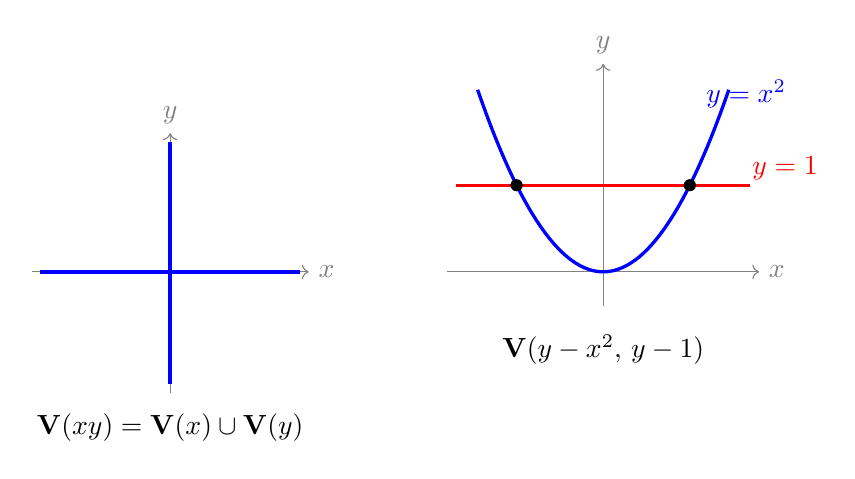
\begin{tikzpicture}[scale=1.1]
  \begin{scope}
    \draw[->,gray] (-1.6,0)--(1.6,0) node[right]{$x$};
    \draw[->,gray] (0,-1.4)--(0,1.6) node[above]{$y$};
    \draw[very thick,blue] (-1.5,0)--(1.5,0);
    \draw[very thick,blue] (0,-1.3)--(0,1.5);
    \node at (0,-1.8) {$\Zero(xy)=\Zero(x)\cup\Zero(y)$};
  \end{scope}
  \begin{scope}[xshift=5cm]
    \draw[->,gray] (-1.8,0)--(1.8,0) node[right]{$x$};
    \draw[->,gray] (0,-0.4)--(0,2.4) node[above]{$y$};
    \draw[very thick,blue,domain=-1.45:1.45,samples=60] plot (\x,{\x*\x});
    \draw[very thick,red] (-1.7,1)--(1.7,1);
    \fill (1,1) circle (2pt) (-1,1) circle (2pt);
    \node[blue] at (1.65,2.05) {$y=x^2$};
    \node[red] at (2.1,1.2) {$y=1$};
    \node at (0,-0.9) {$\Zero(y-x^2,\,y-1)$};
  \end{scope}
\end{tikzpicture}
\caption{和集合と共通部分．積 $xy$ の零点は和集合，連立方程式の零点は共通部分になる．}
\label{fig:ch01-zero-sets}
\end{figure}

\subsection{多項式系によって定義される図形}

$\A^n$ の中で $m$ 個の「独立な」方程式で定まる図形は，直感的には $n-m$ 次元であると期待される．
たとえば $\A^3$ において
\[
  X=\Zero(y-x^2,\ z-x^3)
\]
を考えよう．$X$ の点は $(t,t^2,t^3)$（$t\in k$）と一意にパラメータ表示されるので，$X$ は1次元の曲線である．
これを\textbf{ねじれ三次曲線}（twisted cubic）という．$X$ は2つの曲面 $\Zero(y-x^2)$（放物柱面）と
$\Zero(z-x^3)$ の交わりである．

ところが，「方程式の個数を引けば次元が出る」という素朴な期待はしばしば裏切られる．
\begin{itemize}
  \item $k=\R$ のとき，$\Zero(x^2+y^2)=\{(0,0)\}$ は1個の方程式で定義されるにもかかわらず $0$ 次元である．
        これは実数特有の現象であり，複素数上では $x^2+y^2=(x+iy)(x-iy)$ より $\Zero(x^2+y^2)$ は2直線の和集合（1次元）になる．
  \item $\Zero(x,\ x)=\Zero(x)$ のように，方程式が重複していれば次元は減らない．
  \item より微妙な例として，$\A^3$ の3本の座標軸の和集合 $\Zero(xy,\ yz,\ zx)$ は1次元（余次元2）であるが，
        その定義イデアル $(xy,yz,zx)$ は2個の元では生成できない．このように方程式の個数と余次元が一致しない
        「完全交差でない」例は多数存在する（第7章，第9章）．
\end{itemize}
次元の正確な定義（Krull次元）と，「$m$ 個の方程式で定まる図形の各既約成分の次元は $n-m$ 以上である」という
正しい形の主張は第7章で扱う．
また，代数的集合の全体がある位相（\textbf{Zariski位相}）の閉集合系をなすことを第3章で見る．

\begin{myex}{行列の集合}{ch01-matrices}
$2\times2$ 行列全体を $\A^4$ と同一視する．階数 $\le1$ の行列全体は $\Zero(ad-bc)$ であり，これは $\A^4$ の超曲面（3次元）である．
冪零行列全体は $\Zero(a+d,\ ad-bc)$ であり，「固有多項式 $\lambda^2-(a+d)\lambda+(ad-bc)$ が $\lambda^2$ に等しい」という条件を表す．
これは $\A^4$ の中の2次元の図形（冪零錐）である．
\end{myex}

\exprob{prob:ch01-2-1}
$k=\C$ とし，$\A^2$ において $\Zero(x^2+y^2-1,\ x-y)$ を求めよ．また $\Zero(x^2+y^2-1,\ x^2-y^2)$ を求め，
後者を定義するイデアルが $(x^2-\tfrac12,\ y^2-\tfrac12)$ に等しいことを示せ．

\exprob{prob:ch01-2-2}
$k=\F_p$（$p$ は素数）上で，すべての $a\in k$ に対して $f(a)=0$ を満たす $0$ でない多項式の例を一つ挙げよ
（ヒント：Fermatの小定理）．

%======================================================================
\section{実代数幾何と複素代数幾何}
%======================================================================

\subsection{実数上の代数的集合}

$k=\R$ のとき，代数的集合は我々の直観に最も近い「目に見える」図形である．
しかし同時に，代数的な性質と幾何学的な性質の対応はしばしば崩れる．
典型例は次の3つの曲線である．
\[
  \Zero(x^2+y^2-1),\qquad \Zero(x^2+y^2),\qquad \Zero(x^2+y^2+1).
\]
いずれも「同じ形」の2次方程式で定まるが，実数上ではそれぞれ円・1点・空集合となる（図\ref{fig:ch01-real-circles}）．

\begin{figure}[H]
\centering
\begin{tikzpicture}[scale=0.9]
  \foreach \s/\lab in {0/{$x^2+y^2=1$},4.5/{$x^2+y^2=0$},9/{$x^2+y^2=-1$}}{
    \begin{scope}[xshift=\s cm]
      \draw[->,gray] (-1.6,0)--(1.6,0);
      \draw[->,gray] (0,-1.6)--(0,1.6);
      \node at (0,-2.1) {\lab};
    \end{scope}}
  \draw[very thick,blue] (0,0) circle (1);
  \fill[blue] (4.5,0) circle (2.5pt);
  \node at (9,0.6) {$\emptyset$};
\end{tikzpicture}
\caption{実数上の $x^2+y^2=c$：$c>0$ で円，$c=0$ で1点，$c<0$ で空集合．}
\label{fig:ch01-real-circles}
\end{figure}

実数上の代数的集合には，次のような特有の性質がある．

\begin{myprop}{実数上では1つの方程式で十分}{ch01-real-single}
$f_1,\dots,f_m\in\R[x_1,\dots,x_n]$ に対し，$\R^n$ において
\[
  \Zero(f_1,\dots,f_m)=\Zero(f_1^2+\dots+f_m^2)
\]
が成り立つ．
\end{myprop}

\begin{proof}
実数 $c_1,\dots,c_m$ について，$c_1^2+\dots+c_m^2=0$ と $c_1=\dots=c_m=0$ は同値であることから直ちに従う．
\end{proof}

したがって実数上では「方程式の個数」は幾何学的な意味をもたない．
たとえば $\R^3$ 内の円 $\{x^2+y^2=1,\ z=0\}$ は1つの方程式 $(x^2+y^2-1)^2+z^2=0$ で定義される「超曲面」である．
また，実数上では空でない方程式系と空の方程式系を代数的に区別すること自体が難しい問題であり
（これは Positivstellensatz と呼ばれる実代数幾何学の主題である），本ノートでは深入りしない．

ただし実数上の代数幾何が無意味というわけではない．物理の場面では最終的に実数の量を扱うことが多く，
相空間や配位空間の形状を調べる上で実代数的集合は重要である．本ノートでは，まず複素数上で理論を整え，
実数上の情報は「複素共役で固定される部分」として後から取り出す（1.3.4小節）という立場をとる．

\subsection{複素数上の代数的集合}

$k=\C$ のとき，最も重要な事実は\textbf{代数学の基本定理}である：
定数でない一変数複素係数多項式は必ず $\C$ に根をもつ．
すなわち $\C$ は\textbf{代数閉体}である．これから次元の低い場合について次の主張が得られる．

\begin{myprop}{複素超曲面は空でない}{ch01-complex-nonempty}
$n\ge1$ とし，$f\in\C[x_1,\dots,x_n]$ を定数でない多項式とする．このとき $\Zero(f)\ne\emptyset$ である．
さらに $n\ge2$ ならば $\Zero(f)$ は無限集合である．
\end{myprop}

\begin{proof}
必要なら変数の番号を付け替えて，$f$ は $x_1$ を実際に含むとしてよい．
$f=\sum_{i=0}^dg_i(x_2,\dots,x_n)x_1^i$，$d\ge1$，$g_d\ne0$ と書く．
$n=1$ ならば $g_d$ は $0$ でない定数であり，代数学の基本定理より $f$ は根をもつ．
$n\ge2$ のとき，命題\ref{prop:ch01-poly-function}より $g_d(b_0)\ne0$ となる $b_0\in\C^{n-1}$ が存在する．
さらに，0でないベクトル $e\in\C^{n-1}$ を一つ選ぶと，$t$ の一変数多項式 $g_d(b_0+te)$ は $t=0$ で $0$ でないので
$0$ でない多項式であり，その根は有限個しかない．よって $g_d(b)\ne0$ となる $b$（$=b_0+te$ の形のもの）は無限個存在する．
各そのような $b$ に対して，$f(x_1,b)$ は $x_1$ の $d$ 次多項式であるから根 $a$ をもち，$(a,b)\in\Zero(f)$ となる．
$b$ が異なれば点も異なるので，$\Zero(f)$ は無限集合である．
\end{proof}

この命題は，実数上の $\Zero(x^2+y^2+1)=\emptyset$ のような現象が複素数上では起こらないことを示している．
より一般に，複素数上では「連立方程式系が解をもたないのは，代数的な理由（$1$ が方程式から導かれる）があるときに限る」
という\textbf{弱零点定理}が成り立つ（第4章）．

複素代数的集合を「見る」際には注意が必要である．$\C$ は実2次元であるから，
複素平面曲線 $\Zero(f)\subset\C^2$ は実4次元空間 $\C^2\cong\R^4$ 内の実2次元の曲面である．
たとえば $\Zero(y)\subset\C^2$ は「直線」と呼ばれるが，位相的には平面 $\C\cong\R^2$ である．
したがって複素代数曲線は\textbf{Riemann面}として理解される（第13章）．
本章の図はほとんどが実部分 $\Zero(f)\cap\R^2$ を描いたものであり，これは複素曲線の「一断面」にすぎないことに注意してほしい．

\subsection{実数と複素数における零点の違い}

実数と複素数の違いを，いくつかの観点から比較してみよう．

\paragraph{根の個数．}
一変数 $d$ 次多項式は，複素数上では重複度込めてちょうど $d$ 個の根をもつが，実数上では $0$ 個から $d$ 個まで様々である．
係数を連続的に動かしたとき，実根の個数は不連続に変化しうる（判別式が $0$ を横切るとき，2つの実根が衝突して複素共役な2根になる）．
複素根の個数（重複度込み）は変化しない．
この「数が保存される」という性質は，連続変形のもとで不変な量（交点数，Euler数など）を扱う上で本質的である．

\paragraph{位相の違い：円の複素化．}
複素平面曲線 $C_\C=\{(x,y)\in\C^2\mid x^2+y^2=1\}$ を考える．$u=x+iy$，$v=x-iy$ とおくと
$x^2+y^2=uv$ であるから，
\[
  C_\C\cong\{(u,v)\in\C^2\mid uv=1\}\cong\C^\times=\C\setminus\{0\},\qquad (u,v)\mapsto u
\]
となる（逆写像は $u\mapsto(u,1/u)$）．$\C^\times$ は位相的には円柱 $S^1\times\R$ である
（$u=re^{i\theta}$ に対し $(\theta,\log r)$ を対応させる）．
実部分 $C_\R=C_\C\cap\R^2$ は $v=\bar u$ となる点，すなわち $|u|=1$ の点であり，円柱の「胴回り」の円に相当する
（図\ref{fig:ch01-complex-circle}）．

\begin{figure}[H]
\centering
\begin{tikzpicture}
  \begin{scope}
    \draw[->,gray] (-1.6,0)--(1.6,0) node[right]{$x$};
    \draw[->,gray] (0,-1.6)--(0,1.6) node[above]{$y$};
    \draw[very thick,blue] (0,0) circle (1);
    \node at (0,-2.2) {実部分 $C_\R\cong S^1$};
  \end{scope}
  \begin{scope}[xshift=5.5cm]
    \draw[thick] (-1.2,1.6) ellipse (1.2 and 0.3);
    \draw[thick] (-2.4,1.6)--(-2.4,-1.6);
    \draw[thick] (0,1.6)--(0,-1.6);
    \draw[thick] (-2.4,-1.6) arc (180:360:1.2 and 0.3);
    \draw[thick,dashed,gray] (0,-1.6) arc (0:180:1.2 and 0.3);
    \draw[very thick,blue] (-2.4,0) arc (180:360:1.2 and 0.3);
    \draw[thick,blue,dashed] (0,0) arc (0:180:1.2 and 0.3);
    \node[blue,right] at (0.05,0) {$|u|=1$（実点）};
    \node at (-1.2,2.2) {$|u|\to\infty$};
    \node at (-1.2,-2.25) {$|u|\to0$};
    \node at (-1.2,-2.85) {複素曲線 $C_\C\cong\C^\times$（円柱）};
  \end{scope}
\end{tikzpicture}
\caption{円 $x^2+y^2=1$ の実部分と複素化．複素化は円柱であり，実部分はその胴回りの円である．}
\label{fig:ch01-complex-circle}
\end{figure}

円柱の両端 $|u|\to0$，$|u|\to\infty$ は，射影平面における2つの無限遠点 $[1:\pm i:0]$ に対応する．
これらを付け加えると $C_\C$ は球面 $S^2\cong\PP^1$ になる（第8章，第13章）．
実数上の円がコンパクトであるのに対し複素アフィン曲線は決してコンパクトにならないこと，
そしてコンパクト化するには射影空間が必要であることがこの例からわかる．

\paragraph{双曲線と円．}
実数上では円 $x^2+y^2=1$ と双曲線 $x^2-y^2=1$ は全く異なる形をしている（コンパクトと非コンパクト，連結と非連結）．
しかし複素数上では，座標変換 $y\mapsto iy$ によって両者は同型になる．
実数上の分類（楕円・放物線・双曲線）が複素数上ではより粗い分類に統合されることは，1.4.2小節で再び見る．

\subsection{複素化の意味}

実係数多項式 $f_1,\dots,f_m\in\R[x_1,\dots,x_n]$ に対し，同じ方程式を複素数上で考えた
$X_\C=\Zero(f_1,\dots,f_m)\subset\C^n$ を，実代数的集合 $X_\R=X_\C\cap\R^n$ の\textbf{複素化}という．
$f_i$ の係数は実数なので，複素共役 $\sigma:\C^n\to\C^n$，$\sigma(a)=\bar a$ は $X_\C$ をそれ自身に写す：
\[
  f_i(\bar a)=\overline{f_i(a)}=0.
\]
そして $X_\R$ はちょうど $\sigma$ の固定点集合である．
つまり，\emph{実代数幾何は「複素代数幾何 $+$ 複素共役という対合」}として捉えられる．

複素化の中には，実部分以外にも物理的に意味のある「実の断面」が含まれていることがある．
円 $x^2+y^2=1$ の複素化において，$x\in\R$，$y=i\eta$（$\eta\in\R$）となる点を考えると，
条件は $x^2-\eta^2=1$ となり，これは双曲線である．パラメータで書けば
\[
  (\cos\theta,\ \sin\theta)\ \xrightarrow{\ \theta=i t\ }\ (\cosh t,\ i\sinh t)
\]
であり，回転角 $\theta$ を虚数にする操作が円を双曲線に変える．
これは Euclid 空間の回転群 $SO(2)$ と Lorentz 群 $SO(1,1)$ が，同じ複素群 $SO(2,\C)$ の異なる実形であることの，
最も簡単な現れである．

\begin{physbox}[Wick回転と複素化]
場の量子論における Wick 回転 $t\mapsto -i\tau$ は，Minkowski 計量 $-dt^2+d\vec x^2$ を Euclid 計量 $d\tau^2+d\vec x^2$ に写す．
これは「時間座標を複素化し，複素化された空間の別の実断面を見る」操作に他ならない．
上で見た円と双曲線の関係はその最も簡単な模型である．
一般に，物理量を解析接続して複素領域で考えることで，異なる実断面の間の関係（たとえば Euclid 的な経路積分と
Lorentz 的な時間発展）が見通しよく理解できる．代数幾何学が複素数上で最もよく機能することは，この考え方と相性がよい．
\end{physbox}

\subsection{複素代数幾何が物理に現れる理由}

なぜ理論物理，とりわけ弦理論や超対称ゲージ理論において，\emph{複素}代数幾何がこれほど頻繁に現れるのだろうか．
いくつかの理由を挙げておく．

\begin{enumerate}
  \item \textbf{量子力学は複素数の理論である．}状態ベクトルや確率振幅は複素数値であり，ユニタリ群・複素射影空間
        （純粋状態の空間は $\PP(\mathcal H)$）が自然に現れる．
  \item \textbf{超対称性は正則性をもたらす．}4次元 $\mathcal N=1$ 超対称理論では，超ポテンシャル $W$ はカイラル超場の
        \emph{正則関数}であり，多くの場合多項式である．真空の条件は $\partial W/\partial\phi_i=0$ という多項式方程式になる（1.5.2小節）．
        正則性は非くりこみ定理などの強い制約を生み，厳密な計算を可能にする．
  \item \textbf{2次元の共形対称性は複素構造と結びつく．}弦の世界面は2次元であり，共形構造は Riemann 面の複素構造と同値である
        （第13章）．したがって弦の摂動論は Riemann 面のモジュライ空間上の積分として定式化される．
  \item \textbf{コンパクト化の内部空間は複素多様体である．}超対称性を保つコンパクト化の内部空間として
        Calabi--Yau 多様体が現れ，その多くは射影空間内の多項式方程式で具体的に構成される（1.5.4小節，第15章）．
  \item \textbf{複素数上では数が保存される．}1.3.3小節で見たように，複素数上では解の個数や交点数が変形に対して不変であり，
        これが位相的不変量（指数，Euler数，Gromov--Witten不変量など）と物理量（真空の数，粒子の世代数など）を結びつける．
\end{enumerate}

\begin{physbox}[本ノートにおける複素数の役割]
本ノートでは，第13章以降で複素幾何（複素多様体，Kähler 幾何）と代数幾何の関係を詳しく扱う．
重要な原理は，射影空間内の多項式で定義される図形（射影多様体）は自動的にコンパクト複素多様体になり，
逆に十分よい条件のもとではコンパクト複素多様体が代数的に記述できる（Chowの定理，GAGA）ということである．
これにより，物理で必要な微分幾何学的な量（計量，曲率，ゲージ場）と，代数幾何学的な計算（多項式，次数，交点数）が
結びつけられる．
\end{physbox}

\exprob{prob:ch01-3-1}
$\C^2$ の曲線 $C=\Zero(x^2-y^2-1)$ が $\C^\times$ と全単射に対応することを，具体的な写像を与えて示せ．
また $C\cap\R^2$ はいくつの連結成分をもつか答えよ．

\exprob{prob:ch01-3-2}
実一変数多項式 $f_t(x)=x^3-3x+t$（$t\in\R$）の実根の個数を $t$ の値で分類せよ．
実根の個数が変化する $t$ の値において，$f_t$ は重根をもつことを確かめよ．

%======================================================================
\section{代数幾何学の基本的な例}
%======================================================================

この節では，以後の章で繰り返し登場する基本的な例を図とともに眺める．
各例について (i) 実部分の形，(ii) 複素数上での姿，(iii) 座標環やパラメータ表示といった代数的な記述，の3点に注目する．

\subsection{直線}

平面 $\A^2$ の\textbf{直線}とは，$(a,b)\ne(0,0)$ として一次方程式 $ax+by+c=0$ の零点集合のことである．
直線 $L$ は1点 $p$ と方向ベクトル $v$ を用いて
\[
  \A^1\to L,\qquad t\mapsto p+tv
\]
と全単射にパラメータ表示される．座標環で言えば，たとえば $L=\Zero(y)$ に対して
$k[x,y]/(y)\cong k[x]$ であり，これは「$L$ は $\A^1$ と同型である」ことの代数的な表現である（第5章）．

2本の直線 $L_1:\ a_1x+b_1y=c_1$，$L_2:\ a_2x+b_2y=c_2$ の交わりは，連立一次方程式の解である．
行列式 $a_1b_2-a_2b_1\ne0$ ならばただ1点で交わり，$=0$ ならば平行（交わらないか一致する）である．
「平行な2直線は交わらない」という例外は，射影平面 $\PP^2$ において無限遠直線を付け加えることで解消される：
平行な直線たちは，その方向に対応する無限遠点で交わる（第8章）．

\begin{figure}[H]
\centering
\begin{tikzpicture}[scale=1]
  \begin{scope}
    \draw[->,gray] (-1.8,0)--(1.8,0) node[right]{$x$};
    \draw[->,gray] (0,-1.4)--(0,1.6) node[above]{$y$};
    \draw[very thick,blue] (-1.6,-1.2)--(1.6,1.2);
    \draw[very thick,red] (-1.6,1.0)--(1.6,-0.6);
    \fill (0.457,0.343) circle (2pt);
    \node at (0,-2) {$\det\ne0$：1点で交わる};
  \end{scope}
  \begin{scope}[xshift=5.5cm]
    \draw[->,gray] (-1.8,0)--(1.8,0) node[right]{$x$};
    \draw[->,gray] (0,-1.4)--(0,1.6) node[above]{$y$};
    \draw[very thick,blue] (-1.6,-0.9)--(1.4,1.35);
    \draw[very thick,red] (-1.0,-1.3)--(1.8,0.8);
    \draw[->,dashed,gray] (1.5,1.45)--(2.2,1.97) node[above right]{無限遠点で交わる};
    \node at (0,-2) {$\det=0$：平行};
  \end{scope}
\end{tikzpicture}
\caption{2直線の交わり．平行線は射影平面の無限遠点で交わる．}
\label{fig:ch01-lines}
\end{figure}

一般に，$\A^n$ の\textbf{一次部分多様体}（アフィン部分空間）は連立一次方程式の解集合であり，その次元は線形代数で完全に理解される．
線形代数は「次数1の代数幾何」とみなすことができる．代数幾何学の難しさと面白さは，次数2以上の方程式から生じる．

\subsection{円と二次曲線}

平面の\textbf{二次曲線}（円錐曲線）とは，二次多項式
\[
  f(x,y)=ax^2+bxy+cy^2+dx+ey+g\qquad((a,b,c)\ne(0,0,0))
\]
の零点集合である．実数上では，アフィン変換（平行移動と可逆な一次変換）によって，非退化な二次曲線は
\[
  \text{楕円 } x^2+y^2=1,\qquad \text{放物線 } y=x^2,\qquad \text{双曲線 } x^2-y^2=1
\]
のいずれかに変換できる（ただし $x^2+y^2=-1$ のように実点をもたないものを除く）．
どれになるかは，二次の部分の判別式 $b^2-4ac$ が負・零・正のいずれであるかで決まる．

\begin{figure}[H]
\centering
\begin{tikzpicture}[scale=0.85]
  \begin{scope}
    \draw[->,gray] (-2.2,0)--(2.2,0); \draw[->,gray] (0,-1.6)--(0,1.6);
    \draw[very thick,blue] (0,0) ellipse (1.6 and 1);
    \node at (0,-2.1) {楕円 $b^2-4ac<0$};
  \end{scope}
  \begin{scope}[xshift=5cm,yshift=-1cm]
    \draw[->,gray] (-2.2,0)--(2.2,0); \draw[->,gray] (0,-0.6)--(0,2.6);
    \draw[very thick,blue,domain=-1.55:1.55,samples=60] plot (\x,{\x*\x});
    \node at (0,-1.1) {放物線 $b^2-4ac=0$};
  \end{scope}
  \begin{scope}[xshift=10cm]
    \draw[->,gray] (-2.2,0)--(2.2,0); \draw[->,gray] (0,-1.6)--(0,1.6);
    \draw[very thick,blue,domain=-1.15:1.15,samples=60] plot ({cosh(\x)},{sinh(\x)});
    \draw[very thick,blue,domain=-1.15:1.15,samples=60] plot ({-cosh(\x)},{sinh(\x)});
    \draw[gray,dashed] (-1.6,-1.6)--(1.6,1.6) (-1.6,1.6)--(1.6,-1.6);
    \node at (0,-2.1) {双曲線 $b^2-4ac>0$};
  \end{scope}
\end{tikzpicture}
\caption{実二次曲線の3つの型}
\label{fig:ch01-conics}
\end{figure}

複素数上では，1.3.3小節で見たように楕円と双曲線は区別できなくなり（$y\mapsto iy$），
非退化なアフィン二次曲線は本質的に「$xy=1$ 型」と「$y=x^2$ 型」の2種類になる．
両者の違いは無限遠での振る舞いにある：$xy=1$ 型は無限遠直線と2点で交わり，$y=x^2$ 型は無限遠直線と1点で接する．
射影平面 $\PP^2$ まで考えると，非退化な二次曲線は（複素数上では）すべて互いに射影変換で移りあい，$\PP^1$ と同型になる（第8章）．

\paragraph{円の有理パラメータ表示．}
円 $C:\ x^2+y^2=1$ 上の点 $P=(-1,0)$ を通る傾き $t$ の直線 $y=t(x+1)$ を考える．
これを円の方程式に代入すると $(x+1)\big((1+t^2)x-(1-t^2)\big)=0$ となるので，$P$ 以外の交点は
\begin{equation}\label{eq:ch01-stereo}
  x=\frac{1-t^2}{1+t^2},\qquad y=\frac{2t}{1+t^2}
\end{equation}
である（図\ref{fig:ch01-stereo}）．この直線は $y$ 軸と $(0,t)$ で交わるので，これは $P$ からの\textbf{立体射影}である．
こうして円は，有限個の点を除いて直線と一対一に対応する．このように有理関数でパラメータ表示される曲線を\textbf{有理曲線}という（第10章）．

\begin{figure}[H]
\centering
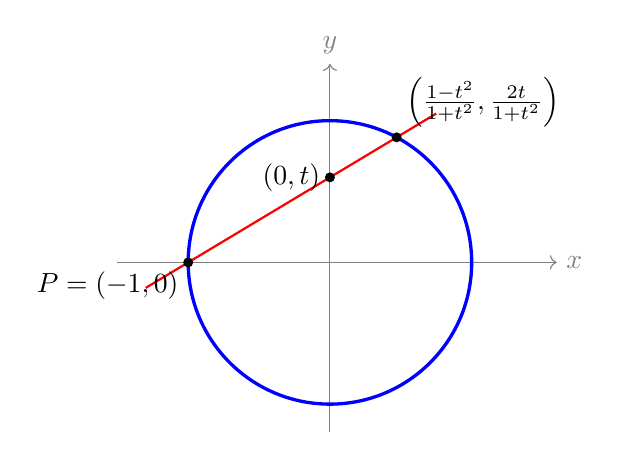
\begin{tikzpicture}[scale=1.8]
  \draw[->,gray] (-1.5,0)--(1.6,0) node[right]{$x$};
  \draw[->,gray] (0,-1.2)--(0,1.4) node[above]{$y$};
  \draw[very thick,blue] (0,0) circle (1);
  \draw[thick,red] (-1.3,-0.18)--(0.75,1.05);
  \fill (-1,0) circle (1pt) node[below left]{$P=(-1,0)$};
  \fill (0,0.6) circle (1pt) node[left]{$(0,t)$};
  \fill (0.4706,0.8824) circle (1pt) node[above right]{$\left(\frac{1-t^2}{1+t^2},\frac{2t}{1+t^2}\right)$};
\end{tikzpicture}
\caption{円の立体射影による有理パラメータ表示}
\label{fig:ch01-stereo}
\end{figure}

式 \eqref{eq:ch01-stereo} は数論的にも興味深い．$t=m/n$ を有理数とすれば $C$ の有理点が得られ，分母を払うと
\[
  (n^2-m^2)^2+(2mn)^2=(n^2+m^2)^2
\]
となって，Pythagoras 数がすべて（定数倍を除いて）得られる．また複素数上では，分母が $0$ になる $t=\pm i$ が
1.3.3小節で見た2つの無限遠点に対応し，$t=\infty$ が点 $P$ に対応する．
したがって複素円 $C_\C$ は $\PP^1$ から2点を除いたもの，すなわち $\C^\times$ と同型であり，1.3.3小節の結果と整合する．

\subsection{放物線}

放物線 $P=\Zero(y-x^2)$ は，多項式 $x^2$ のグラフである．写像
\[
  \A^1\to P,\quad t\mapsto(t,t^2),\qquad P\to\A^1,\quad (x,y)\mapsto x
\]
は互いに逆であり，どちらも多項式で書かれている．したがって $P$ は $\A^1$ と\emph{代数多様体として同型}である（第5章）．
これに対応して，座標環についても
\[
  k[x,y]/(y-x^2)\ \cong\ k[x]
\]
が成り立つ（$y$ を $x^2$ に置き換える写像．2.2.4小節で証明する）．
曲がっている放物線と真っすぐな直線が「同じ」であるというのは奇妙に思えるかもしれないが，
代数幾何学は計量（距離や曲率）ではなく，多項式関数の構造のみを見ているのである．

これと対照的なのが双曲線 $H=\Zero(xy-1)$ である．$H$ の座標環は
\[
  k[x,y]/(xy-1)\ \cong\ k[x,x^{-1}]\qquad(\text{Laurent多項式環})
\]
であり，ここでは $x$ が逆元 $x^{-1}=y$ をもつ．一方，$k[x]$ において逆元をもつのは $0$ でない定数だけである．
環の同型は可逆元を可逆元に写すので，$k[x]\not\cong k[x,x^{-1}]$ であり，したがって $H$ は $\A^1$ と同型ではない．
幾何学的には，$H$ は $x$ 軸への射影によって $\A^1\setminus\{0\}$ と同型であり，「穴が1つ開いた直線」である．
実数上では $H$ は2つの連結成分をもつ（図\ref{fig:ch01-parabola-hyperbola}）が，複素数上では $\C^\times$ は連結である．

\begin{figure}[H]
\centering
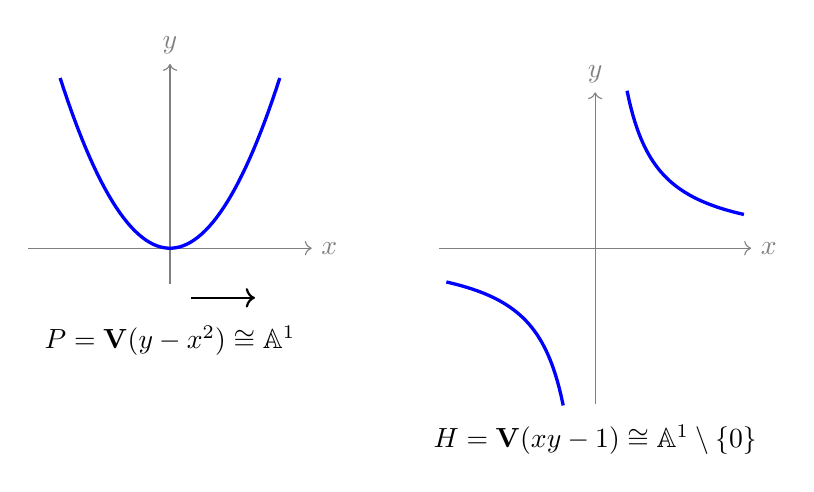
\begin{tikzpicture}[scale=0.9]
  \begin{scope}
    \draw[->,gray] (-2,0)--(2,0) node[right]{$x$}; \draw[->,gray] (0,-0.5)--(0,2.6) node[above]{$y$};
    \draw[very thick,blue,domain=-1.55:1.55,samples=60] plot (\x,{\x*\x});
    \draw[thick,->] (0.3,-0.7)--(1.2,-0.7);
    \node at (0,-1.3) {$P=\Zero(y-x^2)\cong\A^1$};
  \end{scope}
  \begin{scope}[xshift=6cm]
    \draw[->,gray] (-2.2,0)--(2.2,0) node[right]{$x$}; \draw[->,gray] (0,-2.2)--(0,2.2) node[above]{$y$};
    \draw[very thick,blue,domain=0.45:2.1,samples=60] plot (\x,{1/\x});
    \draw[very thick,blue,domain=-2.1:-0.45,samples=60] plot (\x,{1/\x});
    \node at (0,-2.7) {$H=\Zero(xy-1)\cong\A^1\setminus\{0\}$};
  \end{scope}
\end{tikzpicture}
\caption{放物線と双曲線．前者は直線と同型，後者は原点を除いた直線と同型である．}
\label{fig:ch01-parabola-hyperbola}
\end{figure}

\begin{myex}{グラフは常にアフィン空間と同型}{ch01-graph}
一般に多項式 $g\in k[x_1,\dots,x_n]$ のグラフ $\Gamma_g=\Zero(x_{n+1}-g(x_1,\dots,x_n))\subset\A^{n+1}$ は，
射影 $(x_1,\dots,x_{n+1})\mapsto(x_1,\dots,x_n)$ によって $\A^n$ と同型である．
座標環では $k[x_1,\dots,x_{n+1}]/(x_{n+1}-g)\cong k[x_1,\dots,x_n]$ に対応する．
\end{myex}

\subsection{楕円曲線}

次数3の平面曲線の中で最も重要なのが\textbf{楕円曲線}である．標数が $2,3$ でない体上では，楕円曲線は
\textbf{Weierstrass形式}
\begin{equation}\label{eq:ch01-weierstrass}
  y^2=x^3+ax+b,\qquad 4a^3+27b^2\ne0
\end{equation}
で表される（正確には，これに射影平面の無限遠点 $O=[0:1:0]$ を1つ付け加えたものである）．
条件 $4a^3+27b^2\ne0$ は，右辺の三次式が重根をもたないことと同値であり，曲線が\textbf{特異点}をもたない（滑らかである）
ことを保証する（第7章）．量 $\Delta=-16(4a^3+27b^2)$ を\textbf{判別式}と呼ぶ．

典型例 $E:\ y^2=x^3-x=x(x-1)(x+1)$ を考えよう（$a=-1,\ b=0$，$4a^3+27b^2=-4\ne0$）．
$y^2\ge0$ でなければならないので，実部分は $x^3-x\ge0$，すなわち $-1\le x\le0$ または $x\ge1$ の範囲にあり，
図\ref{fig:ch01-elliptic}左のように「卵形」と「無限に伸びる枝」の2つの連結成分をもつ．
一般に，$x^3+ax+b$ が相異なる3つの実根をもつとき（$4a^3+27b^2<0$）実部分は2成分，実根が1つのとき（$4a^3+27b^2>0$）1成分である．

\begin{figure}[H]
\centering
\begin{tikzpicture}[scale=0.95]
  \begin{scope}
    \draw[->,gray] (-1.6,0)--(2.5,0) node[right]{$x$}; \draw[->,gray] (0,-3)--(0,3) node[above]{$y$};
    \draw[very thick,blue,domain=0:180,samples=90,smooth]
      plot ({-sin(\x)*sin(\x)},{sin(\x)*cos(\x)*sqrt(1+sin(\x)*sin(\x))});
    \draw[very thick,blue,domain=-1.1:1.1,samples=60,smooth]
      plot ({1+\x*\x},{\x*sqrt((1+\x*\x)*(2+\x*\x))});
    \node at (0.4,-3.5) {$y^2=x^3-x$（滑らか）};
  \end{scope}
  \begin{scope}[xshift=5cm]
    \draw[->,gray] (-1.6,0)--(1.8,0) node[right]{$x$}; \draw[->,gray] (0,-3)--(0,3) node[above]{$y$};
    \draw[very thick,blue,domain=-1.45:1.45,samples=80,smooth]
      plot ({\x*\x-1},{\x*(\x*\x-1)});
    \fill[red] (0,0) circle (2pt);
    \node at (0.1,-3.5) {$y^2=x^2(x+1)$（結節点）};
  \end{scope}
  \begin{scope}[xshift=9.5cm]
    \draw[->,gray] (-0.6,0)--(2,0) node[right]{$x$}; \draw[->,gray] (0,-3)--(0,3) node[above]{$y$};
    \draw[very thick,blue,domain=-1.35:1.35,samples=80,smooth]
      plot ({\x*\x},{\x*\x*\x});
    \fill[red] (0,0) circle (2pt);
    \node at (0.7,-3.5) {$y^2=x^3$（尖点）};
  \end{scope}
\end{tikzpicture}
\caption{楕円曲線 $y^2=x^3-x$ の実部分（左）と，判別式が $0$ になる退化した三次曲線（中・右）．
赤い点は特異点である．}
\label{fig:ch01-elliptic}
\end{figure}

判別式が $0$ になると曲線は特異点をもつ．$y^2=x^2(x+1)$ は原点で自分自身と交わる\textbf{結節点}（node）をもち，
$y^2=x^3$ は原点で尖る\textbf{尖点}（cusp）をもつ（図\ref{fig:ch01-elliptic}）．
これらの特異三次曲線はそれぞれ
\[
  t\mapsto(t^2-1,\ t(t^2-1)),\qquad t\mapsto(t^2,\ t^3)
\]
とパラメータ表示される有理曲線である．
一方，滑らかな楕円曲線は有理関数でパラメータ表示することができない（有理曲線ではない）．

楕円曲線の真価は複素数上で現れる．複素楕円曲線（無限遠点を含む）は，位相的には\textbf{トーラス} $S^1\times S^1$ であり，
複素解析的には格子 $\Lambda=\Z\omega_1+\Z\omega_2\subset\C$ による商 $\C/\Lambda$ と同型である
（Weierstrass の $\wp$ 関数を用いて $(x,y)=(\wp(z),\wp'(z)/2)$ の形で与えられる．定数の規格化は流儀による）．
さらに，楕円曲線上の点には「2点を通る直線と曲線の第3の交点」を用いて\emph{加法}が定義され，アーベル群の構造が入る．
これらの詳細は第13章（Riemann面としての楕円曲線）と第17章（楕円曲線と物理，F理論）で扱う．

\begin{physbox}[楕円曲線と物理]
楕円曲線は，トーラス上の2次元共形場理論（弦の1ループ振幅）において，トーラスの複素構造 $\tau$ として現れる．
また $\mathcal N=2$ 超対称ゲージ理論の低エネルギー有効理論を記述する Seiberg--Witten 曲線（1.5.1小節），
およびF理論において結合定数 $\tau=C_0+ie^{-\phi}$ を幾何学的に表すファイバーとしても現れる（第17章）．
物理において楕円曲線の「形」を変えることは，結合定数などの物理的パラメータを変えることに対応する．
\end{physbox}

\subsection{高次元超曲面}

$\A^n$ の超曲面 $\Zero(f)$ は，1つの方程式で定義される $n-1$ 次元の図形である．
$n=3$ の場合の二次曲面の典型例として，実数 $\varepsilon$ をパラメータとする族
\[
  Q_\varepsilon=\Zero(x^2+y^2-z^2-\varepsilon)\subset\A^3
\]
を考えよう．実数上では，$\varepsilon>0$ のとき一葉双曲面，$\varepsilon=0$ のとき円錐，$\varepsilon<0$ のとき二葉双曲面である
（図\ref{fig:ch01-quadrics}）．

\begin{figure}[H]
\centering
\begin{tikzpicture}[scale=0.75]
  % one-sheeted hyperboloid
  \begin{scope}
    \draw[very thick,blue,domain=-1.2:1.2,samples=50,smooth] plot ({cosh(\x)},{sinh(\x)});
    \draw[very thick,blue,domain=-1.2:1.2,samples=50,smooth] plot ({-cosh(\x)},{sinh(\x)});
    \draw[thick,blue] (0,1.509) ellipse (1.811 and 0.35);
    \draw[thick,blue] (-1.811,-1.509) arc (180:360:1.811 and 0.35);
    \draw[thick,blue,dashed] (1.811,-1.509) arc (0:180:1.811 and 0.35);
    \draw[thick,blue] (-1,0) arc (180:360:1 and 0.2);
    \draw[thick,blue,dashed] (1,0) arc (0:180:1 and 0.2);
    \node at (0,-2.6) {$\varepsilon>0$：一葉双曲面};
  \end{scope}
  % cone
  \begin{scope}[xshift=5.5cm]
    \draw[very thick,blue] (-1.5,1.5)--(1.5,-1.5) (1.5,1.5)--(-1.5,-1.5);
    \draw[thick,blue] (0,1.5) ellipse (1.5 and 0.3);
    \draw[thick,blue] (-1.5,-1.5) arc (180:360:1.5 and 0.3);
    \draw[thick,blue,dashed] (1.5,-1.5) arc (0:180:1.5 and 0.3);
    \fill[red] (0,0) circle (3pt);
    \node at (0,-2.6) {$\varepsilon=0$：円錐（特異点あり）};
  \end{scope}
  % two-sheeted hyperboloid
  \begin{scope}[xshift=11cm]
    \draw[very thick,blue,domain=-1.1:1.1,samples=50,smooth] plot ({sinh(\x)},{cosh(\x)});
    \draw[very thick,blue,domain=-1.1:1.1,samples=50,smooth] plot ({sinh(\x)},{-cosh(\x)});
    \draw[thick,blue] (0,1.669) ellipse (1.336 and 0.3);
    \draw[thick,blue] (-1.336,-1.669) arc (180:360:1.336 and 0.3);
    \draw[thick,blue,dashed] (1.336,-1.669) arc (0:180:1.336 and 0.3);
    \node at (0,-2.6) {$\varepsilon<0$：二葉双曲面};
  \end{scope}
\end{tikzpicture}
\caption{二次曲面の族 $x^2+y^2-z^2=\varepsilon$ の実部分（縦軸が $z$ 軸）．$\varepsilon=0$ で原点に特異点が現れる．}
\label{fig:ch01-quadrics}
\end{figure}

実数上ではこの3つは位相的に全く異なる（連結成分の個数も違う）が，複素数上では $\varepsilon\ne0$ のものはすべて互いに同型であり
（変数を $\sqrt{\varepsilon}$ 倍すればよい），$\varepsilon=0$ のときだけ原点に\textbf{特異点}をもつ円錐が現れる．
すなわち，複素数上では「滑らかな曲面の族が，ある値で特異な曲面に退化する」という描像になる．
これは第7章で扱う特異点の典型例であり，その高次元版（3次元のconifold特異点 $x^2+y^2+z^2+w^2=0$）は
弦理論における幾何学的遷移で中心的な役割を果たす（第17章）．

より一般に，$\PP^n$ の中の $d$ 次超曲面として，\textbf{Fermat超曲面}
\[
  x_0^d+x_1^d+\dots+x_n^d=0
\]
が重要な例を与える．$n=2$，$d=3$ では楕円曲線，$n=3$，$d=4$ では \textbf{K3曲面}，
$n=4$，$d=5$ では\textbf{Quintic三次元多様体}となる．
後二者は「$d=n+1$」という共通の条件を満たしており，これが Calabi--Yau 多様体になるための条件である（1.5.4小節，第15章）．
射影空間内の超曲面の一般論は第9章で扱う．

\exprob{prob:ch01-4-1}
双曲線 $x^2-y^2=1$ 上の点 $(-1,0)$ を通る傾き $t$ の直線を用いて，双曲線の有理パラメータ表示を求めよ．
どの $t$ の値で分母が $0$ になるか，その幾何学的な意味（漸近線との関係）とともに答えよ．

\exprob{prob:ch01-4-2}
$y^2=x^3+ax+b$ について，右辺の三次式 $x^3+ax+b$ が重根をもつことと $4a^3+27b^2=0$ が同値であることを示せ．
（ヒント：重根 $\alpha$ は $\alpha^3+a\alpha+b=0$ かつ $3\alpha^2+a=0$ を満たす．）

%======================================================================
\section{代数幾何学と理論物理}
%======================================================================

この節では，本ノートの第V部（第13章〜第17章）で扱う物理への応用を先取りして概観する．
ここでの説明は直観的なものであり，正確な定義や議論は該当する章で行う．
読者は，ここで出てくる用語の意味がまだわからなくても気にせず，「代数幾何学がどのような場面で必要になるか」をつかんでほしい．

\subsection{ゲージ理論における幾何学}

Maxwell 理論や Yang--Mills 理論といったゲージ理論は，幾何学的には\textbf{主束}上の\textbf{接続}の理論である．
ゲージ場 $A_\mu$ は接続，場の強さ $F_{\mu\nu}$ は曲率，ゲージ変換は束の自己同型に対応する（第14章）．
これだけなら微分幾何学の話であるが，次のような場面で代数幾何学が本質的に現れる．

\begin{itemize}
  \item \textbf{インスタントン．}4次元 Euclid 空間上の反自己双対 Yang--Mills 方程式の解（インスタントン）は，
        ADHM 構成によって，有限次元の行列に関する二次方程式の解を群作用で割ったものとして記述される．
        つまり無限次元の偏微分方程式の解空間が，有限次元の\emph{代数的な}方程式で記述される．
  \item \textbf{正則ベクトル束．}複素曲面上の反自己双対接続は，（適切な条件のもとで）正則ベクトル束と対応する
        （Donaldson--Uhlenbeck--Yau の定理，第14章）．微分方程式の問題が複素代数幾何の問題に翻訳される．
  \item \textbf{Seiberg--Witten理論．}4次元 $\mathcal N=2$ 超対称 $SU(2)$ ゲージ理論の低エネルギー有効理論は，
        パラメータ $u$ をもつ楕円曲線の族（Seiberg--Witten 曲線），たとえばある規格化のもとで
        \[
          y^2=(x^2-u)^2-\Lambda^4
        \]
        によって完全に決定される．ここで $u$ は真空のモジュライ空間の座標であり，楕円曲線が特異になる $u=\pm\Lambda^2$ において
        新たな粒子（モノポールやダイオン）が質量ゼロになる．
\end{itemize}

\subsection{真空の分類と代数的構造}

4次元 $\mathcal N=1$ 超対称理論において，カイラル超場 $\phi_1,\dots,\phi_n$ の超ポテンシャル $W(\phi)$ は正則関数であり，
多くの模型では多項式である．スカラーポテンシャルは $V=\sum_i|\partial W/\partial\phi_i|^2$（ゲージ相互作用がない場合）であり，
超対称な真空（$V=0$）は
\[
  \frac{\partial W}{\partial\phi_1}=\dots=\frac{\partial W}{\partial\phi_n}=0
\]
という\emph{多項式方程式系}の解，すなわち代数的集合である．

\begin{myex}{真空のモジュライの退化}{ch01-vacua}
3つのカイラル超場 $\Phi,X,Y$ と超ポテンシャル $W=\lambda\Phi(XY-\mu^2)$（$\lambda\ne0$）を考える．F項条件は
\[
  \partial_\Phi W=\lambda(XY-\mu^2)=0,\qquad \partial_XW=\lambda\Phi Y=0,\qquad \partial_YW=\lambda\Phi X=0.
\]
$\mu\ne0$ のとき，第1式より $X,Y\ne0$ であるから $\Phi=0$ となり，真空の集合は $\{\Phi=0,\ XY=\mu^2\}\cong\C^\times$ である．
$\mu=0$ のとき，真空の集合は
\[
  \{XY=0,\ \Phi X=0,\ \Phi Y=0\}=\{X=Y=0\}\cup\{\Phi=X=0\}\cup\{\Phi=Y=0\}
\]
となり，原点で交わる3本の直線の和集合になる．パラメータ $\mu$ を $0$ に近づけると，真空の空間は滑らかな曲線から
特異点をもつ図形へと退化し，原点で新たな方向（$\Phi$ 方向）が開く（図\ref{fig:ch01-vacua}）．
\end{myex}

\begin{figure}[H]
\centering
\begin{tikzpicture}[scale=0.9]
  \begin{scope}
    \draw[->,gray] (-2.2,0)--(2.2,0) node[right]{$X$}; \draw[->,gray] (0,-2.2)--(0,2.2) node[above]{$Y$};
    \draw[very thick,blue,domain=0.3:2.1,samples=60] plot (\x,{0.6/\x});
    \draw[very thick,blue,domain=-2.1:-0.3,samples=60] plot (\x,{0.6/\x});
    \node at (0,-2.7) {$\mu\ne0$：$XY=\mu^2$（$\Phi=0$）};
  \end{scope}
  \begin{scope}[xshift=6.5cm]
    \draw[very thick,blue] (-2,0)--(2,0) node[right]{$X$};
    \draw[very thick,blue] (0,-2)--(0,2) node[above]{$Y$};
    \draw[very thick,red] (-1.2,-1.0)--(1.2,1.0) node[above right]{$\Phi$};
    \fill (0,0) circle (2.5pt);
    \node at (0,-2.7) {$\mu=0$：3本の直線};
  \end{scope}
\end{tikzpicture}
\caption{例\ref{ex:ch01-vacua}の真空の集合（実部分の模式図）．}
\label{fig:ch01-vacua}
\end{figure}

ゲージ対称性がある場合には，さらに D 項条件を課してゲージ群で割る必要がある．
多くの場合，この操作は「F項条件の解をゲージ群の複素化 $G_\C$ で割る」という代数的な商と一致し，
真空のモジュライ空間は\emph{ゲージ不変な正則多項式}を座標とする代数多様体として記述される．
たとえば $U(1)$ ゲージ理論で電荷 $\pm1$ のカイラル超場 $Q,\tilde Q$ をもち $W=0$ のとき，
真空のモジュライ空間はゲージ不変量 $M=Q\tilde Q$ を座標とする $\C$ である．
ゲージ不変な多項式が有限個の元で生成されることは Hilbert の不変式論の帰結であり，その背後には第2章で扱う
Hilbert の基底定理がある．真空のモジュライ空間と，それを代数的な商として記述する考え方は第14章（14.6.5小節）と第16章で触れる．

\subsection{弦理論におけるコンパクト化}

超弦理論は10次元時空で整合的に定義される．我々の観測する4次元時空を得るには，残りの6次元を小さなコンパクト空間 $K$ に
巻き上げる必要がある：
\[
  M_{10}=M_4\times K_6.
\]
これを\textbf{コンパクト化}という．最も簡単な例として，5次元の質量ゼロのスカラー場を半径 $R$ の円 $S^1$ 上にコンパクト化すると，
円方向の運動量が量子化され，4次元では質量 $|n|/R$（$n\in\Z$）の粒子の無限個の塔（Kaluza--Klein モード）が現れる．
$R$ が小さければ $n\ne0$ のモードは重く，低エネルギーでは $n=0$ のモードだけが残る．

一般に，4次元の低エネルギー有効理論の粒子の種類や相互作用は，内部空間 $K$ の幾何学的・位相的性質
（Betti数，交点数，ベクトル束の Chern 類など）によって決まる．
たとえば，ヘテロティック弦理論の Calabi--Yau コンパクト化では，フェルミオンの世代数が $K$ の Euler 数の半分の絶対値 $|\chi(K)|/2$
で与えられるという古典的な結果がある（標準埋め込みの場合）．
このように，\emph{物理的な量が幾何学的な不変量として計算される}ことがコンパクト化の要点であり，
その不変量を計算する道具として代数幾何学が用いられる（第15章）．

\subsection{Calabi--Yau多様体}

4次元で $\mathcal N=1$ 超対称性を保つコンパクト化の条件を調べると，内部空間 $K$ は
（フラックスなどがない最も簡単な状況で）\textbf{Calabi--Yau 3次元多様体}であることが要請される
（Candelas--Horowitz--Strominger--Witten，1985年）．
Calabi--Yau 多様体の大まかな定義は「コンパクトな Kähler 多様体で，第一 Chern 類が消えるもの」であり，
Calabi 予想（Yau により証明）によって，このとき Ricci 平坦な Kähler 計量が存在する．

\begin{note}
Calabi--Yau 多様体の定義は文献によって異なる．標準束が自明であること，第一Chern類（実係数）が $0$ であること，
ホロノミー群が $SU(n)$ に含まれる（あるいは一致する）こと，$h^{p,0}=0$（$0<p<n$）を課すかどうか，などの流儀がある．
単連結性などの条件のもとでこれらは同値になるが，一般には一致しない．詳しくは第15章で論じる．
\end{note}

代数幾何学の立場から重要なのは，Calabi--Yau 多様体の多くが\emph{射影空間内の多項式方程式によって具体的に構成できる}ことである．
$\PP^n$ の滑らかな $d$ 次超曲面が（標準束が自明という意味で）Calabi--Yau になる条件は $d=n+1$ である（第15章）．
したがって
\begin{itemize}
  \item 1次元：$\PP^2$ の三次曲線（楕円曲線），
  \item 2次元：$\PP^3$ の四次曲面（K3曲面），
  \item 3次元：$\PP^4$ の五次超曲面（Quintic），たとえば $x_0^5+x_1^5+x_2^5+x_3^5+x_4^5=0$
\end{itemize}
が Calabi--Yau 多様体の基本例となる．Quintic の Hodge 数は $h^{1,1}=1$，$h^{2,1}=101$ であり，Euler 数は
$\chi=2(h^{1,1}-h^{2,1})=-200$ である．
重み付き射影空間内の超曲面や完全交差を用いると，さらに多くの例が得られる（第15章）．

\subsection{モジュライ空間と物理的自由度}

Calabi--Yau 多様体は1つではなく，連続的なパラメータをもつ族として存在する．
「ある種類の幾何学的対象の同型類全体」がなす空間を\textbf{モジュライ空間}と呼ぶ（第16章）．

最も簡単な例は楕円曲線である．Weierstrass 形式 \eqref{eq:ch01-weierstrass} の楕円曲線 $y^2=x^3+ax+b$ の同型類は，
\textbf{$j$不変量}
\[
  j=1728\,\frac{4a^3}{4a^3+27b^2}
\]
によって完全に分類される（代数閉体上）．すなわち，$(a,b)$ という2つのパラメータのうち，同型で移りあう分（$(a,b)\mapsto(\lambda^4a,\lambda^6b)$）
を除いた1次元の自由度 $j$ が楕円曲線の「形」を表し，楕円曲線のモジュライ空間は $j$ 直線 $\A^1$ である．
複素解析的には，これはトーラス $\C/(\Z+\Z\tau)$ の複素構造 $\tau$ を $\SL(2,\Z)$ で割ったものに対応する（第13章，第17章）．

Quintic Calabi--Yau の場合にも同様の勘定ができる．5変数の5次単項式は $126$ 個あるから（例\ref{ex:ch01-monomial-count}），
5次多項式の係数は126個のパラメータをもつ．このうち $\GL_5(\C)$ による座標変換（次元25）で移りあうものは同型であるから，
本質的なパラメータの数は
\[
  126-25=101
\]
であり，これはちょうど Hodge 数 $h^{2,1}=101$ に一致する．これが Quintic の\textbf{複素構造モジュライ}の次元である．
同様の勘定で，$\PP^2$ の三次曲線は $\binom{5}{2}-9=10-9=1$，$\PP^3$ の四次曲面は $\binom{7}{3}-16=35-16=19$ 個の
パラメータをもつ．

\begin{physbox}[モジュライ場]
コンパクト化において，内部空間 $K$ の形や大きさを表すモジュライは，4次元時空の各点で値をとる場，すなわち\textbf{モジュライ場}となる．
モジュライの方向にはポテンシャルが（摂動論的には）生じないので，モジュライ場は4次元で質量ゼロのスカラー場として現れる．
Quintic の場合，101個の複素構造モジュライと1個の Kähler モジュライ（大きさ）が，それぞれ4次元のスカラー場の自由度を与える．
観測とのつじつまを合わせるにはこれらの場に質量を与える機構（モジュライ安定化）が必要であり，これは現代の弦理論の重要な課題である．
複素構造モジュライと Kähler モジュライを入れ替える双対性がミラー対称性であり（第17章），
モジュライ空間の幾何学そのものが物理の重要な研究対象となっている．詳細は第16章で扱う．
\end{physbox}

\exprob{prob:ch01-5-1}
$y^2=x^3+ax+b$ において $(a,b)\mapsto(\lambda^4a,\lambda^6b)$（$\lambda\ne0$）としても $j$ 不変量が変わらないことを確かめよ．
また，この変換が座標変換 $(x,y)\mapsto(\lambda^2x,\lambda^3y)$ から生じることを示せ．

\exprob{prob:ch01-5-2}
$\PP^n$ の $d$ 次超曲面の定義多項式の係数の個数から $\GL_{n+1}$ の次元を引いた数 $\binom{n+d}{d}-(n+1)^2$ を，
$(n,d)=(2,3),(3,4),(4,5)$ について計算し，本文の値と一致することを確かめよ．

\section*{問題の解答}
\addcontentsline{toc}{section}{問題の解答}

\exsol{prob:ch01-1-1}
$y=x^2+c$ を $x^2+y^2=1$ に代入すると，$x$ の四次方程式
\[
  x^4+(2c+1)x^2+(c^2-1)=0
\]
を得る．逆にこの解 $x$ に対して $y=x^2+c$ と定めれば交点が得られ，交点と解 $x$ は一対一に対応する．
ヒントに従って $x^2=y-c$ を円の式に代入すると
\[
  g(y):=y^2+y-(1+c)=0
\]
となる．各交点の $y$ 座標は $g(y)=0$ の根であり，逆に根 $y$ に対して $x^2=y-c$ を満たす $x$ をとれば交点が得られる．
したがって実の交点を数えるには，$g$ の実根 $y$ のうち $y\ge c$ を満たすものを調べればよい
（$y>c$ なら $x=\pm\sqrt{y-c}$ の2点，$y=c$ なら $x=0$ の1点が対応する）．

$g$ の判別式は $1+4(1+c)=4c+5$ であり，実根は $y_\pm=\dfrac{-1\pm\sqrt{4c+5}}{2}$，$y_-\le-\tfrac12\le y_+$ である．
また $g(c)=c^2-1$ である．$g$ は下に凸なので，$c$ が2根の間にあるのは $g(c)<0$ のとき，2根より小さいのは $g(c)>0$ かつ $c<-\frac12$ のとき，
2根より大きいのは $g(c)>0$ かつ $c>-\frac12$ のときである．これより次のように場合分けされる．
\begin{itemize}
  \item $c<-\frac54$：実根がないので交点は $0$ 個．
  \item $c=-\frac54$：重根 $y=-\frac12$ で $y-c=\frac34>0$．交点は $(\pm\frac{\sqrt3}2,-\frac12)$ の $2$ 個（それぞれで接する）．
  \item $-\frac54<c<-1$：$g(c)>0$，$c<-\frac12$ なので $c<y_-<y_+$．交点は $4$ 個．
  \item $c=-1$：$g(y)=y(y+1)$ で根は $-1=c$ と $0$．交点は $(0,-1)$ と $(\pm1,0)$ の $3$ 個．
  \item $-1<c<1$：$g(c)<0$ なので $y_-<c<y_+$．$y_+$ のみが寄与し，交点は $2$ 個．
  \item $c=1$：$g(y)=(y-1)(y+2)$ で $y_+=1=c$．交点は $(0,1)$ の $1$ 個．
  \item $c>1$：$g(c)>0$，$c>-\frac12$ なので $y_-<y_+<c$．交点は $0$ 個．
\end{itemize}

複素数の範囲では，上の $x$ の四次方程式は最高次係数が $1$ なので，代数学の基本定理により重複度を込めてちょうど $4$ 個の根をもち，
各根 $x$ に交点 $(x,x^2+c)$ がただ一つ対応する．よって交点は重複度込みで $c$ によらず $4$ 個である．
ヒントの方法で言えば，$g(y)=0$ が重複度込みで $2$ 根をもち，各根 $y$ に対して $x^2=y-c$ が重複度込みで $2$ 根をもつので $2\times2=4$ である．
たとえば $c=-1$ では $x^4-x^2=x^2(x-1)(x+1)$ で $x=0$ が二重根（点 $(0,-1)$ で接する），
$c=1$ では $x^4+3x^2=x^2(x^2+3)$ で $x=0$ が二重根，残り2個は虚の交点 $(\pm\sqrt3\,i,-2)$，
$c=-\frac54$ では $x^4-\frac32x^2+\frac9{16}=(x^2-\frac34)^2$ で2点がそれぞれ二重に数えられる．

\exsol{prob:ch01-1-2}
グラフ $\Gamma=\{(x,\log x)\mid x>0\}$ が代数的集合 $\Zero(f_1,\dots,f_m)$（$f_i\in\R[x,y]$）に等しいと仮定する．
$F=f_1^2+\dots+f_m^2$ とおくと，実数の範囲では $F(P)=0\iff f_1(P)=\dots=f_m(P)=0$ なので $\Gamma=\Zero(F)$ である．
$\Gamma\ne\R^2$ だから $F\ne0$ である．

$F=\sum_{i,j}a_{ij}x^iy^j$ と書き，$x=e^t$（$t\in\R$）を代入すると，すべての $t\in\R$ に対して
\[
  0=F(e^t,t)=\sum_{i=0}^{N}b_i(t)\,e^{it},\qquad b_i(t)=\sum_ja_{ij}t^j\in\R[t]
\]
が成り立つ．$F\ne0$ なので $b_i\ne0$ となる $i$ があり，そのような $i$ の最大値を改めて $N$ とする．両辺を $e^{Nt}$ で割ると
\[
  b_N(t)=-\sum_{i=0}^{N-1}b_i(t)\,e^{-(N-i)t}.
\]
$t\to+\infty$ のとき，右辺の各項は（多項式）$\times$（指数関数的に減少する関数）なので $0$ に収束する．
一方，$0$ でない多項式 $b_N(t)$ は $t\to+\infty$ で $0$ に収束しない（定数なら $0$ でない定数，次数 $1$ 以上なら $\pm\infty$ に発散する）．
これは矛盾である．よって $\Gamma$ はどの代数的集合とも一致しない．
本質は，$\log x$（あるいは $e^t$）が多項式の関係式を満たさない，すなわち超越的な関数であることにある．

\exsol{prob:ch01-2-1}
$\Zero(x^2+y^2-1,\ x-y)$：$y=x$ を代入して $2x^2=1$，$x=\pm\frac1{\sqrt2}$．よって
\[
  \Zero(x^2+y^2-1,\ x-y)=\Bigl\{\bigl(\tfrac1{\sqrt2},\tfrac1{\sqrt2}\bigr),\ \bigl(-\tfrac1{\sqrt2},-\tfrac1{\sqrt2}\bigr)\Bigr\}.
\]
$\Zero(x^2+y^2-1,\ x^2-y^2)$：$f=x^2+y^2-1$，$g=x^2-y^2$ とおくと
\[
  x^2-\tfrac12=\tfrac12(f+g),\qquad y^2-\tfrac12=\tfrac12(f-g),\qquad
  f=\bigl(x^2-\tfrac12\bigr)+\bigl(y^2-\tfrac12\bigr),\qquad g=\bigl(x^2-\tfrac12\bigr)-\bigl(y^2-\tfrac12\bigr).
\]
前の2式から $x^2-\frac12,\ y^2-\frac12$ は $f,g$ の多項式係数の一次結合であり，後の2式からその逆も成り立つ．
したがって $f,g$ の生成するイデアルと $x^2-\frac12,\ y^2-\frac12$ の生成するイデアルは等しい：
\[
  (x^2+y^2-1,\ x^2-y^2)=\bigl(x^2-\tfrac12,\ y^2-\tfrac12\bigr).
\]
零点集合はイデアルのみで決まるので
\[
  \Zero(x^2+y^2-1,\ x^2-y^2)=\Zero\bigl(x^2-\tfrac12,\ y^2-\tfrac12\bigr)=\Bigl\{\bigl(\pm\tfrac1{\sqrt2},\ \pm\tfrac1{\sqrt2}\bigr)\Bigr\}
\]
（複号任意の4点）である．幾何学的には，$x^2-y^2=(x-y)(x+y)$ なので，これは円と二直線 $y=\pm x$ の交点である．

\exsol{prob:ch01-2-2}
$f=x^p-x\in\F_p[x]$ とすればよい．$f$ は次数 $p$ の多項式なので零多項式ではない．
一方 Fermat の小定理により，すべての $a\in\F_p$ について $a^p=a$（$a=0$ では自明，$a\ne0$ では $a^{p-1}=1$）だから $f(a)=0$ である．
実際 $x^p-x=\prod_{a\in\F_p}(x-a)$ であり，$\F_p$ のすべての元を根にもつ．
これは，有限体上では「多項式」と「多項式関数」を区別しなければならないことを示している．

\exsol{prob:ch01-3-1}
$x^2-y^2=(x+y)(x-y)$ なので，$C$ は $(x+y)(x-y)=1$ で定まる．写像
\[
  \Phi\colon C\to\C^\times,\quad (x,y)\mapsto u=x+y,\qquad
  \Psi\colon\C^\times\to C,\quad u\mapsto\Bigl(\frac{u+u^{-1}}2,\ \frac{u-u^{-1}}2\Bigr)
\]
を考える．$(x,y)\in C$ なら $(x+y)(x-y)=1$ より $u=x+y\ne0$ なので $\Phi$ は well-defined である．
また $\Psi(u)$ について $x+y=u$，$x-y=u^{-1}$ なので $x^2-y^2=u\cdot u^{-1}=1$，すなわち $\Psi(u)\in C$．
$\Phi\circ\Psi(u)=u$ は明らか．逆に $(x,y)\in C$ に対し $x-y=(x+y)^{-1}=u^{-1}$ なので
$x=\frac{u+u^{-1}}2$，$y=\frac{u-u^{-1}}2$，すなわち $\Psi\circ\Phi=\mathrm{id}_C$．よって $\Phi$ は全単射である．
（本文の双曲線 $xy=1$ の場合と同じく，$C$ は $\C^\times$ と同型であり，複素数上では連結である．）

$C\cap\R^2$ は実双曲線 $x^2-y^2=1$ である．$x^2=1+y^2\ge1$ より $x\ge1$ または $x\le-1$ であり，
それぞれの部分は $y\mapsto(\pm\sqrt{1+y^2},y)$ によって $\R$ と同相なので連結である．一方 $\{x\ge1\}$ と $\{x\le-1\}$ は直線 $x=0$ で分離される．
よって $C\cap\R^2$ の連結成分は $2$ 個である．上の対応では，実の点は $u\in\R^\times$ に対応し，$\R^\times=\R_{>0}\sqcup\R_{<0}$ の2成分がそのまま2本の枝になる．

\exsol{prob:ch01-3-2}
$f_t'(x)=3x^2-3=3(x-1)(x+1)$ なので，$f_t$ は $x=-1$ で極大値 $f_t(-1)=t+2$，$x=1$ で極小値 $f_t(1)=t-2$ をとり，
$x\to\pm\infty$ で $f_t(x)\to\pm\infty$ である．中間値の定理と増減から
\begin{itemize}
  \item $|t|<2$（極大値 $>0$，極小値 $<0$）：相異なる実根が $3$ 個，
  \item $|t|=2$：相異なる実根が $2$ 個（うち1つは重根），
  \item $|t|>2$（極大値と極小値が同符号）：実根は $1$ 個
\end{itemize}
となる．実根の個数が変化するのは $t=\pm2$ であり，このとき
\[
  f_2(x)=x^3-3x+2=(x-1)^2(x+2),\qquad f_{-2}(x)=x^3-3x-2=(x+1)^2(x-2)
\]
となって，確かに重根 $x=1$，$x=-1$ をもつ．三次式 $x^3+px+q$ の判別式 $-4p^3-27q^2$ を用いれば，
$-4(-3)^3-27t^2=27(4-t^2)$ が $0$ になる $t$ がちょうど $\pm2$ であることからも確かめられる．
重根は二つの実根が合流して（$|t|>2$ 側では）一組の共役な虚根に変わる瞬間を表している．

\exsol{prob:ch01-4-1}
点 $(-1,0)$ を通る傾き $t$ の直線 $y=t(x+1)$ を $x^2-y^2=1$ に代入すると
\[
  x^2-1-t^2(x+1)^2=(x+1)\bigl[(x-1)-t^2(x+1)\bigr]=0.
\]
因子 $x+1$ は既知の交点 $(-1,0)$ に対応し，もう一つの交点は $(1-t^2)x=1+t^2$ から得られる：
\[
  x=\frac{1+t^2}{1-t^2},\qquad y=t(x+1)=\frac{2t}{1-t^2}.
\]
実際 $(1+t^2)^2-(2t)^2=(1-t^2)^2$ なので $x^2-y^2=1$ を満たす．
逆に双曲線上の点 $(x,y)\ne(-1,0)$ では $x\ne-1$（$x=-1$ なら $y=0$）なので $t=y/(x+1)$ が定まり，上の式で表される．
（点 $(-1,0)$ 自身は，そこでの接線である垂直線 $x=-1$，すなわち $t=\infty$ に対応する．）

分母が $0$ になるのは $t=\pm1$ のときである．このとき直線 $y=\pm(x+1)$ は双曲線の漸近線 $y=\pm x$ と平行であり，
上の式で $(1-t^2)x=1+t^2$ が $0=2$ となって解をもたない．すなわち2番目の交点が存在せず，「無限遠に逃げた」と解釈できる．
射影平面（第8章以降）で考えると，これは漸近線方向の無限遠点 $[1:\pm1:0]$ が双曲線上にあり，$t=\pm1$ がそれらに対応していることを意味する．

\exsol{prob:ch01-4-2}
$f(x)=x^3+ax+b$ とする（係数体は標数 $2,3$ でない体，たとえば $\C$ とする）．
まず，$\alpha$ が $f$ の重根であることと $f(\alpha)=f'(\alpha)=0$ が同値であることに注意する．
実際 $f=(x-\alpha)^2g$ なら $f'=2(x-\alpha)g+(x-\alpha)^2g'$ より $f'(\alpha)=0$．
逆に $f(\alpha)=0$ なら $f=(x-\alpha)h$ と書けて $f'=h+(x-\alpha)h'$ なので，$f'(\alpha)=0$ なら $h(\alpha)=0$，すなわち $(x-\alpha)^2\mid f$．
したがって重根 $\alpha$ は
\[
  \alpha^3+a\alpha+b=0,\qquad 3\alpha^2+a=0
\]
を満たす $\alpha$ に他ならない（$\C$ で考えれば根は必ず存在する）．

\textbf{$a=0$ の場合．}第2式から $\alpha=0$，第1式から $b=0$．逆に $a=b=0$ なら $f=x^3$ は重根をもつ．
よって重根をもつ $\iff b=0\iff4a^3+27b^2=0$．

\textbf{$a\ne0$ の場合．}重根 $\alpha$ があるとする．第2式より $\alpha^2=-\frac a3$ なので第1式は
$\alpha(\alpha^2+a)+b=\frac{2a}3\alpha+b=0$，すなわち $\alpha=-\dfrac{3b}{2a}$．これを第2式に代入して
\[
  3\cdot\frac{9b^2}{4a^2}+a=\frac{27b^2+4a^3}{4a^2}=0,
\]
よって $4a^3+27b^2=0$．逆に $4a^3+27b^2=0$ のとき $\alpha=-\frac{3b}{2a}$ とおけば，上の計算から $3\alpha^2+a=0$ であり，
\[
  \alpha^3+a\alpha+b=\alpha(\alpha^2+a)+b=\alpha\cdot\frac{2a}3+b=-b+b=0
\]
となるので，$\alpha$ は重根である．以上で同値性が示された．

\exsol{prob:ch01-5-1}
$a'=\lambda^4a$，$b'=\lambda^6b$ とおくと
\[
  4a'^3+27b'^2=\lambda^{12}(4a^3+27b^2),\qquad
  j(a',b')=1728\,\frac{4\lambda^{12}a^3}{\lambda^{12}(4a^3+27b^2)}=1728\,\frac{4a^3}{4a^3+27b^2}=j(a,b)
\]
であり，$j$ は変わらない（$4a^3+27b^2\ne0$ も保たれる）．

次に $(X,Y)=(\lambda^2x,\lambda^3y)$ とおく．$(x,y)$ が $y^2=x^3+ax+b$ を満たすならば
\[
  Y^2=\lambda^6y^2=\lambda^6x^3+\lambda^6ax+\lambda^6b=X^3+(\lambda^4a)X+\lambda^6b
\]
となり，$(X,Y)$ は $Y^2=X^3+a'X+b'$ を満たす．逆変換 $(x,y)=(\lambda^{-2}X,\lambda^{-3}Y)$ も同じ形なので，
この座標変換は曲線 $y^2=x^3+ax+b$ と $y^2=x^3+a'x+b'$ の間の全単射（どちらの向きも多項式で書ける同型）を与える．
したがってパラメータの変換 $(a,b)\mapsto(\lambda^4a,\lambda^6b)$ は座標変換 $(x,y)\mapsto(\lambda^2x,\lambda^3y)$ から生じている．
この変換で $x$ は重さ $2$，$y$ は重さ $3$，$a$ は重さ $4$，$b$ は重さ $6$ をもち，$a^3$ と $b^2$ がともに重さ $12$ なので，
その比である $j$ が不変量になる．

\exsol{prob:ch01-5-2}
$n+1$ 変数の $d$ 次単項式の個数は $\binom{n+d}{d}$，$\dim\GL_{n+1}=(n+1)^2$ である．
\begin{itemize}
  \item $(n,d)=(2,3)$：$\binom{5}{3}-3^2=10-9=1$．
  \item $(n,d)=(3,4)$：$\binom{7}{4}-4^2=35-16=19$．
  \item $(n,d)=(4,5)$：$\binom{9}{5}-5^2=126-25=101$．
\end{itemize}
本文の値（三次曲線 $1$，四次曲面 $19$，Quintic $101$）と一致する（$\binom52=\binom53$，$\binom73=\binom74$ に注意）．
三次曲線の $1$ は楕円曲線の $j$ 不変量の1次元に，四次曲面（K3曲面）の $19$ は代数的 K3 曲面の複素構造モジュライの次元に，
$101$ は Quintic の $h^{2,1}$ に対応している．

なお，超曲面は定義多項式の定数倍によらないので，正確には「係数の空間 $\binom{n+d}{d}$ 次元から定数倍の $1$ を引き，
$\mathrm{PGL}_{n+1}$（次元 $(n+1)^2-1$）で割る」と数えるべきであるが，
$\bigl(\binom{n+d}{d}-1\bigr)-\bigl((n+1)^2-1\bigr)=\binom{n+d}{d}-(n+1)^2$ なので結果は同じである
（$\GL_{n+1}$ のスカラー行列が多項式を定数倍することに対応する）．

\chapter{可換環論の基礎}\label{ch:ch02}

\begin{chapterlead}
第1章で見たように，代数幾何学では図形 $X$ をその上の多項式関数のなす環 $k[X]$ によって調べる．
本章では，そのために必要な可換環論の基礎をまとめる．
環と環準同型（2.1節，2.2節），イデアル（2.3節），素イデアルと極大イデアル（2.4節），剰余環（2.5節），
多項式環（2.6節），Noether性とHilbertの基底定理（2.7節）を順に扱う．
各概念について，それが幾何学的に何を意味するか（たとえば「極大イデアル $=$ 点」「素イデアル $=$ 既約な図形」
「剰余環 $=$ 図形上の関数環」）を常に意識しながら進む．
群・環・体の最も基本的な定義については付録Bも参照されたい．
\end{chapterlead}

%======================================================================
\section{環の定義と基本構造}
%======================================================================

\subsection{環の定義}

\begin{mydef}{環}{ch02-ring}
集合 $R$ に二つの演算，和 $+:R\times R\to R$ と積 $\cdot:R\times R\to R$ が与えられ，次を満たすとき，$(R,+,\cdot)$ を\textbf{環}という．
\begin{enumerate}
  \item $(R,+)$ はアーベル群である．すなわち和は結合的かつ可換で，零元 $0$ が存在し，各 $a$ に加法逆元 $-a$ が存在する．
  \item 積は結合的である：$(ab)c=a(bc)$．
  \item 分配法則：$a(b+c)=ab+ac$，$(a+b)c=ac+bc$．
  \item 積に関する単位元 $1$ が存在する：$1\cdot a=a\cdot1=a$．
\end{enumerate}
\end{mydef}

条件 (4) を課さない流儀もある（2.1.3小節）が，本ノートでは特に断らない限り環は単位元をもつものとする．
定義から次の基本的な性質が導かれる．

\begin{myprop}{環の基本性質}{ch02-ring-basic}
環 $R$ の任意の元 $a,b$ に対して，次が成り立つ．
\begin{enumerate}
  \item $0\cdot a=a\cdot0=0$．
  \item $(-a)b=a(-b)=-(ab)$，特に $(-1)a=-a$．
  \item $(-a)(-b)=ab$．
\end{enumerate}
\end{myprop}

\begin{proof}
(1) 分配法則より $0\cdot a=(0+0)a=0\cdot a+0\cdot a$．両辺に $-(0\cdot a)$ を加えて $0\cdot a=0$．$a\cdot 0=0$ も同様．
(2) $ab+(-a)b=(a+(-a))b=0\cdot b=0$ より $(-a)b=-(ab)$．もう一方も同様．
(3) (2)を二回用いて $(-a)(-b)=-(a(-b))=-(-(ab))=ab$．
\end{proof}

これらは「当たり前」に見えるが，すべて公理から導かれる性質であることが重要である．
抽象的な環（たとえば多項式を何かで割った環）においても，普段の計算規則が安心して使えることを保証している．

\subsection{可換環と非可換環}

すべての $a,b\in R$ について $ab=ba$ が成り立つ環を\textbf{可換環}という．

\begin{myex}{可換環と非可換環}{ch02-comm-noncomm}
(1) 整数環 $\Z$，有理数体 $\Q$，実数体 $\R$，複素数体 $\C$，多項式環 $k[x_1,\dots,x_n]$ は可換環である．

(2) 体 $k$ 上の $n\times n$ 行列全体 $M_n(k)$ は，行列の和と積で環をなすが，$n\ge2$ のとき可換ではない．
実際
\[
  \begin{pmatrix}0&1\\0&0\end{pmatrix}\begin{pmatrix}0&0\\1&0\end{pmatrix}=\begin{pmatrix}1&0\\0&0\end{pmatrix}
  \ne\begin{pmatrix}0&0\\0&1\end{pmatrix}=\begin{pmatrix}0&0\\1&0\end{pmatrix}\begin{pmatrix}0&1\\0&0\end{pmatrix}.
\]

(3) 四元数 $\mathbb H=\{a+bi+cj+dk\}$（$i^2=j^2=k^2=ijk=-1$）は，$ij=k=-ji$ であるから非可換である．
ただし $0$ でないすべての元が逆元をもつ（斜体）．
\end{myex}

\begin{physbox}[可換性と古典・量子]
量子力学の観測量の代数は非可換である．たとえば一自由度の正準交換関係 $[\hat x,\hat p]=i\hbar$ から生成される代数
（Weyl代数）は非可換環である．$\hbar\to0$ の古典極限で，この代数は相空間上の関数環 $\C[x,p]$ という可換環になる．
代数幾何学が扱うのはこの可換な側であり，可換環 $R$ を「ある空間上の関数環」とみなすことが本ノートの基本的な見方である．
なお，超対称理論で現れる Grassmann 数の代数（$\theta_i\theta_j=-\theta_j\theta_i$）は「超可換」と呼ばれる別の構造であり，
本ノートでは扱わない．
\end{physbox}

\textbf{以下，本ノートでは「環」といえば単位元をもつ可換環を意味する．}
非可換環を扱うときは，その都度明示する．

\subsection{単位元を持つ環}

単位元 $1$ は存在すれば一意である（$1,1'$ がともに単位元なら $1=1\cdot1'=1'$）．
単位元をもたない環の例として，偶数全体 $2\Z$ がある．これは和と積について閉じており，環の公理 (1)〜(3) を満たすが，単位元をもたない．
後で見るように，$2\Z$ は $\Z$ の\emph{イデアル}であり（2.3節），単位元をもたない「環」の多くはイデアルとして自然に理解される．

$1=0$ となる環は $\{0\}$ のみである（$a=1\cdot a=0\cdot a=0$）．これを\textbf{零環}という．
零環は幾何学的には「空集合上の関数環」に対応する．

\begin{mydef}{可逆元・整域・体}{ch02-unit-domain}
$R$ を環とする．
\begin{enumerate}
  \item $ab=1$ となる $b\in R$ が存在する $a$ を\textbf{可逆元}（単元）という．可逆元全体 $R^\times$ は積について群をなす．
  \item $a\ne0$ で，ある $b\ne0$ に対して $ab=0$ となる $a$ を\textbf{零因子}という．
  \item ある $m\ge1$ に対して $a^m=0$ となる $a$ を\textbf{冪零元}という．
  \item $R\ne0$ で，零因子をもたない環を\textbf{整域}という．
  \item $R\ne0$ で，$0$ 以外のすべての元が可逆である環を\textbf{体}という．
\end{enumerate}
\end{mydef}

体は整域である：$a\ne0$，$ab=0$ ならば $b=a^{-1}ab=0$．また $0$ でない冪零元は零因子である
（$a^m=0$ で $m$ を最小にとれば $a\cdot a^{m-1}=0$，$a^{m-1}\ne0$）．

\begin{myex}{$\Z/6\Z$ と $\Z/5\Z$}{ch02-zmod}
$\Z/6\Z=\{\bar0,\bar1,\dots,\bar5\}$ では $\bar2\cdot\bar3=\bar0$ であるから $\bar2,\bar3$ は零因子であり，整域ではない．
可逆元は $\bar1,\bar5$ のみである．一方 $\Z/5\Z$ では $0$ でないすべての元が可逆であり（$\bar2\cdot\bar3=\bar1$，$\bar4\cdot\bar4=\bar1$），体である．
一般に $\Z/n\Z$ が体であることと $n$ が素数であることは同値である（2.4節）．
$\Z/8\Z$ では $\bar2^3=\bar0$ であり，$\bar2$ は冪零元である．
\end{myex}

幾何学的に言えば，零因子は「図形が複数の部分からなる」ことを，冪零元は「図形が重複した構造をもつ」ことを反映している．
たとえば $k[x,y]/(xy)$（2本の座標軸の関数環）では $x\cdot y=0$ であり，$x$ は $y$ 軸上で，$y$ は $x$ 軸上で消えている．
これは2.5.3小節で詳しく見る．

\subsection{部分環}

\begin{mydef}{部分環}{ch02-subring}
環 $R$ の部分集合 $S$ が，$1\in S$ を含み，和・差・積について閉じているとき，$S$ を $R$ の\textbf{部分環}という．
\end{mydef}

部分環は，$R$ の演算を制限することでそれ自身環になる．$1\in S$ を要求することに注意する．
この条件のため，たとえば $2\Z$ は $\Z$ の部分環ではない．

\begin{myex}{部分環の例}{ch02-subring-ex}
(1) $\Z\subset\Q\subset\R\subset\C$ はそれぞれ部分環である．

(2) \textbf{Gauss整数環} $\Z[i]=\{a+bi\mid a,b\in\Z\}$ は $\C$ の部分環である．

(3) $k$ を体とし，$k[x]$ の部分集合
\[
  k[x^2,x^3]=\{a_0+a_2x^2+a_3x^3+a_4x^4+\cdots\}
\]
（$x$ の一次の項をもたない多項式全体）は部分環である．実際，$x$ の一次の項をもたない多項式同士の積も一次の項をもたない．
この環は尖点をもつ曲線 $y^2=x^3$ の座標環と同型である（2.2.5小節）．
「一次の項がない」という条件が，原点で曲線が尖っていることに対応している．

(4) $R$ の部分集合 $T$ に対し，$T$ を含む最小の部分環（$T$ を含む部分環すべての共通部分）を $T$ が\textbf{生成する部分環}という．
$R$ が $S$ を部分環として含み，$a_1,\dots,a_n\in R$ のとき，$S\cup\{a_1,\dots,a_n\}$ が生成する部分環を $S[a_1,\dots,a_n]$ と書く．
これは $a_1,\dots,a_n$ の $S$ 係数多項式として書ける元全体である．たとえば $\Z[\sqrt2]=\{a+b\sqrt2\mid a,b\in\Z\}$．
\end{myex}

\subsection{環の例}

本ノートで頻繁に用いる環の例をまとめておく．

\begin{enumerate}
  \item \textbf{整数環} $\Z$．最も基本的な整域であり，あらゆる環 $R$ に対して唯一の環準同型 $\Z\to R$ が存在する（2.2.1小節）．
  \item \textbf{剰余環} $\Z/n\Z$．$n$ が素数 $p$ のとき有限体 $\F_p$ になる．
  \item \textbf{多項式環} $R[x_1,\dots,x_n]$．代数幾何学の主役である（2.6節）．
  \item \textbf{関数環}．位相空間 $X$ 上の実数値連続関数全体 $C(X)$ は，各点ごとの和と積で可換環をなす．
        $X$ が2点以上からなるとき，$C(X)$ は一般に零因子をもつ（台が交わらない2つの関数の積は $0$）．
  \item \textbf{直積環} $R_1\times R_2$．成分ごとの演算で環をなし，単位元は $(1,1)$ である．
        $e_1=(1,0)$，$e_2=(0,1)$ は $e_i^2=e_i$，$e_1e_2=0$，$e_1+e_2=1$ を満たす（\textbf{冪等元}）．
        幾何学的には，直積環は2つの空間の\emph{非交和}上の関数環に対応し，冪等元は各連結成分上で $1$，他で $0$ の関数である．
  \item \textbf{双対数の環} $k[\varepsilon]=k[x]/(x^2)$．$\varepsilon^2=0$ を満たす元 $\varepsilon$ をもつ．
        $f(a+\varepsilon)=f(a)+f'(a)\varepsilon$ が成り立つことから，接ベクトルや無限小変形を代数的に扱う道具となる（第7章，第12章，第16章）．
  \item \textbf{形式的冪級数環} $k[[x]]$．無限和 $\sum_{i\ge0}a_ix^i$ 全体であり，定数項が $0$ でない元は可逆である
        （例：$(1-x)^{-1}=1+x+x^2+\cdots$）．原点の「無限小近傍」上の関数環とみなせる（第6章）．
  \item \textbf{二次整数環} $\Z[\sqrt{-5}]=\{a+b\sqrt{-5}\mid a,b\in\Z\}$．素因数分解の一意性が成り立たない例として2.6.4小節で用いる．
\end{enumerate}

\exprob{prob:ch02-1-1}
$\Z/12\Z$ の可逆元，零因子，冪零元をすべて求めよ．

\exprob{prob:ch02-1-2}
双対数の環 $k[\varepsilon]$（$\varepsilon^2=0$）において，多項式 $f\in k[x]$ と $a\in k$ に対し $f(a+b\varepsilon)=f(a)+bf'(a)\varepsilon$ が成り立つことを示せ．
また $a+b\varepsilon$ が可逆であるための必要十分条件を求めよ．

%======================================================================
\section{環準同型}
%======================================================================

\subsection{環準同型の定義}

\begin{mydef}{環準同型}{ch02-hom}
環 $R,S$ の間の写像 $\varphi:R\to S$ が，任意の $a,b\in R$ に対して
\[
  \varphi(a+b)=\varphi(a)+\varphi(b),\qquad \varphi(ab)=\varphi(a)\varphi(b),\qquad \varphi(1)=1
\]
を満たすとき，$\varphi$ を\textbf{環準同型}という．
\end{mydef}

加法についての準同型性から $\varphi(0)=0$，$\varphi(-a)=-\varphi(a)$ が従う．
条件 $\varphi(1)=1$ は積の準同型性からは従わない（零写像を除外するために必要である）ので，定義に含めている．

\begin{myex}{環準同型の例}{ch02-hom-ex}
(1) 自然な射影 $\Z\to\Z/n\Z$，$a\mapsto\bar a$．

(2) \textbf{代入準同型}．$a\in k^n$ に対して $\mathrm{ev}_a:k[x_1,\dots,x_n]\to k$，$f\mapsto f(a)$．
これは「関数 $f$ の点 $a$ での値をとる」写像であり，代数幾何学で最も基本的な準同型である．

(3) 複素共役 $\C\to\C$，$z\mapsto\bar z$．

(4) 部分環の包含写像 $S\hookrightarrow R$．

(5) 非例：$\Z\to\Z$，$a\mapsto2a$ は加法を保つが，$2(ab)\ne(2a)(2b)$ となりうるし，$1\mapsto2\ne1$ である．
\end{myex}

任意の環 $R$ に対して，環準同型 $\Z\to R$ はただ一つ存在する．実際 $\varphi(1)=1$ から，$n>0$ に対して
$\varphi(n)=1+\dots+1$（$n$ 個），$\varphi(-n)=-\varphi(n)$ と決まってしまう．
この準同型の核は $n\Z$（$n\ge0$）の形をしており（2.3.4小節），この $n$ を $R$ の\textbf{標数}という．
$\Q,\R,\C$ の標数は $0$，$\F_p$ の標数は $p$ である．整域の標数は $0$ か素数である．

\subsection{核と像}

\begin{mydef}{核と像}{ch02-ker-im}
環準同型 $\varphi:R\to S$ に対して，
\[
  \Ker\varphi=\{a\in R\mid\varphi(a)=0\},\qquad \Img\varphi=\{\varphi(a)\mid a\in R\}
\]
をそれぞれ $\varphi$ の\textbf{核}，\textbf{像}という．
\end{mydef}

\begin{myprop}{核と像の性質}{ch02-ker-im-prop}
$\varphi:R\to S$ を環準同型とする．
\begin{enumerate}
  \item $\Img\varphi$ は $S$ の部分環である．
  \item $\Ker\varphi$ は加法について閉じており，さらに任意の $r\in R$，$a\in\Ker\varphi$ に対して $ra\in\Ker\varphi$ を満たす．
\end{enumerate}
\end{myprop}

\begin{proof}
(1) $1=\varphi(1)\in\Img\varphi$．$\varphi(a)\pm\varphi(b)=\varphi(a\pm b)$，$\varphi(a)\varphi(b)=\varphi(ab)$ より閉じている．
(2) $a,b\in\Ker\varphi$ ならば $\varphi(a+b)=0$，$\varphi(-a)=0$．また $\varphi(ra)=\varphi(r)\varphi(a)=\varphi(r)\cdot0=0$．
\end{proof}

性質 (2) を満たす部分集合を\textbf{イデアル}と呼ぶ（2.3節）．つまり\emph{環準同型の核はイデアルである}．
核は一般に部分環ではないことに注意しよう（$\varphi\ne$ 零写像で $S\ne0$ なら $1\notin\Ker\varphi$）．

\begin{myex}{代入準同型の核}{ch02-ev-kernel}
$a\in k$ に対し $\mathrm{ev}_a:k[x]\to k$ の核は，$f(a)=0$ となる多項式全体である．
因数定理（2.6.1小節）より，これは $x-a$ の倍数全体 $(x-a)=\{(x-a)g\mid g\in k[x]\}$ に一致する．
同様に，$a=(a_1,\dots,a_n)\in k^n$ に対して
\[
  \Ker(\mathrm{ev}_a)=(x_1-a_1,\dots,x_n-a_n)
\]
が成り立つ（問\ref{prob:ch02-2-1}）．これは「点 $a$ で消える関数全体」であり，第1章で $\m_a$ と書いたものである．
\end{myex}

\subsection{単射・全射・同型}

\begin{myprop}{単射性の判定}{ch02-injective}
環準同型 $\varphi:R\to S$ が単射であるための必要十分条件は $\Ker\varphi=\{0\}$ である．
\end{myprop}

\begin{proof}
単射ならば $\varphi(a)=0=\varphi(0)$ から $a=0$．逆に $\Ker\varphi=0$ とし，$\varphi(a)=\varphi(b)$ とすれば $\varphi(a-b)=0$ より $a=b$．
\end{proof}

\begin{mydef}{同型}{ch02-iso}
環準同型 $\varphi:R\to S$ が全単射であるとき，$\varphi$ を\textbf{同型写像}といい，$R$ と $S$ は\textbf{同型}であるといって $R\cong S$ と書く．
\end{mydef}

全単射な環準同型の逆写像は自動的に環準同型になる：$\varphi(\varphi^{-1}(a)\varphi^{-1}(b))=ab$ より $\varphi^{-1}(ab)=\varphi^{-1}(a)\varphi^{-1}(b)$，和も同様．
同型な環は「元の名前の付け方が違うだけ」であり，環論的性質（整域であること，イデアルの構造など）をすべて共有する．

\begin{myex}{同型の例}{ch02-iso-ex}
(1) $\Z/6\Z\cong\Z/2\Z\times\Z/3\Z$，$\bar a\mapsto(a\bmod 2,\ a\bmod 3)$．これは中国剰余定理（2.3.5小節）の特別な場合である．

(2) 体からの環準同型 $\varphi:K\to S$（$S\ne0$）は常に単射である．実際 $a\ne0$ ならば $1=\varphi(a)\varphi(a^{-1})$ より $\varphi(a)\ne0$．

(3) $\Z[i]\cong\Z[x]/(x^2+1)$，$\R[x]/(x^2+1)\cong\C$（2.5節）．
\end{myex}

\subsection{環の同型定理}

イデアル $I\subset R$ に対して，剰余類 $a+I=\{a+x\mid x\in I\}$ 全体の集合 $R/I$ には
\[
  (a+I)+(b+I)=(a+b)+I,\qquad (a+I)(b+I)=ab+I
\]
によって環の構造が入る．これを\textbf{剰余環}という．演算が代表元の取り方によらないことの確認を含め，
剰余環の構成は2.5.1小節で詳しく述べる．ここでは同型定理を先に述べておく．
自然な射影 $\pi:R\to R/I$，$a\mapsto a+I$ は全射環準同型で，$\Ker\pi=I$ である．

\begin{mythm}{準同型定理（第一同型定理）}{ch02-first-iso}
$\varphi:R\to S$ を環準同型とする．このとき
\[
  \bar\varphi:R/\Ker\varphi\ \xrightarrow{\ \sim\ }\ \Img\varphi,\qquad a+\Ker\varphi\mapsto\varphi(a)
\]
は well-defined な環の同型写像である．特に $\varphi$ が全射ならば $R/\Ker\varphi\cong S$．
\end{mythm}

\begin{proof}
$I=\Ker\varphi$ とおく．$a+I=b+I$ ならば $a-b\in I$ なので $\varphi(a)=\varphi(b)$；よって $\bar\varphi$ は well-defined．
環準同型であることは $\varphi$ が準同型であることから直ちに従う．全射性は明らか．
$\bar\varphi(a+I)=0$ ならば $a\in I$ すなわち $a+I=0+I$ なので，$\Ker\bar\varphi=0$ であり単射．
\end{proof}

\[
\begin{tikzcd}
  R \arrow[r,"\varphi"] \arrow[d,"\pi"'] & S\\
  R/\Ker\varphi \arrow[r,"\bar\varphi","\sim"'] & \Img\varphi \arrow[u,hook]
\end{tikzcd}
\]

\begin{myex}{放物線の座標環}{ch02-parabola}
$\varphi:k[x,y]\to k[x]$ を $x\mapsto x$，$y\mapsto x^2$ で定まる準同型とする（$f(x,y)\mapsto f(x,x^2)$）．
$\varphi$ は全射である．核を求めよう．明らかに $y-x^2\in\Ker\varphi$ である．
任意の $f\in k[x,y]$ を $k[x][y]$ の元とみて，$y$ についての一次式 $y-x^2$（$y$ について最高次係数 $1$）で割り算すると
\[
  f(x,y)=(y-x^2)q(x,y)+r(x),\qquad r\in k[x]
\]
と書ける（$y$ に $x^2$ を代入した余りが $r(x)=f(x,x^2)$ である）．$f\in\Ker\varphi$ ならば $0=\varphi(f)=r(x)$ なので
$f=(y-x^2)q$ となる．よって $\Ker\varphi=(y-x^2)$ であり，準同型定理より
\[
  k[x,y]/(y-x^2)\cong k[x].
\]
これは第1章1.4.3小節で予告した「放物線は直線と同型」という主張の代数的な証明である．
\end{myex}

準同型定理に加えて，次の二つの同型定理と対応定理がよく用いられる．証明はいずれも準同型定理を適切な写像に適用すればよい．

\begin{mythm}{第二・第三同型定理}{ch02-iso-thms}
$R$ を環とする．
\begin{enumerate}
  \item $A\subset R$ を部分環，$I\subset R$ をイデアルとすると，$A+I=\{a+x\mid a\in A,\ x\in I\}$ は部分環，$A\cap I$ は $A$ のイデアルであり，
        \[
          A/(A\cap I)\cong(A+I)/I.
        \]
  \item $I\subset J$ を $R$ のイデアルとすると，$J/I=\{x+I\mid x\in J\}$ は $R/I$ のイデアルであり，
        \[
          (R/I)\big/(J/I)\cong R/J.
        \]
\end{enumerate}
\end{mythm}

\begin{proof}
(1) 合成 $A\hookrightarrow A+I\to(A+I)/I$ は全射で，核は $A\cap I$ である．準同型定理を適用すればよい．
(2) $R/I\to R/J$，$a+I\mapsto a+J$ は（$I\subset J$ より）well-defined な全射準同型で，核は $J/I$ である．準同型定理を適用すればよい．
\end{proof}

(2) は「$I$ で割ってから $J/I$ で割るのは，一度に $J$ で割るのと同じ」という意味である．
幾何学的には，$\Zero(J)\subset\Zero(I)$ であり，図形 $\Zero(I)$ の中で部分図形 $\Zero(J)$ を切り出すことに対応する．

\subsection{多項式環の環準同型}

多項式環からの環準同型は，変数の行き先だけで決まる．

\begin{myprop}{多項式環の普遍性}{ch02-poly-universal}
$R,S$ を環，$\psi:R\to S$ を環準同型，$s_1,\dots,s_n\in S$ とする．このとき，環準同型
$\Phi:R[x_1,\dots,x_n]\to S$ で，$\Phi|_R=\psi$ かつ $\Phi(x_i)=s_i$（$i=1,\dots,n$）を満たすものがただ一つ存在する．
\end{myprop}

\begin{proof}
存在：$\Phi\big(\sum c_\alpha x^\alpha\big)=\sum\psi(c_\alpha)s_1^{\alpha_1}\cdots s_n^{\alpha_n}$ と定めれば，$S$ の可換性より環準同型になる．
一意性：環準同型は和と積を保つので，$R$ の元と $x_i$ の行き先が決まれば，それらの多項式の行き先は上の式に決まってしまう．
\end{proof}

特に，$k$ 上の多項式環 $k[x_1,\dots,x_n]$ から $k$ を含む環 $A$ への $k$ 上の準同型（$k$ の元を動かさないもの，\textbf{$k$代数準同型}）は，
$x_i$ の行き先 $a_i\in A$ を任意に指定することで一意に定まる．$A=k$ のときが代入準同型 $\mathrm{ev}_a$ である．

\paragraph{多項式写像と引き戻し．}
多項式 $F_1,\dots,F_n\in k[x_1,\dots,x_m]$ によって写像 $F=(F_1,\dots,F_n):\A^m\to\A^n$ が定まる．
このとき，$\A^n$ 上の関数 $g(y_1,\dots,y_n)$ を $F$ で引き戻した $g\circ F$ は $\A^m$ 上の多項式関数であり，
\[
  F^*:k[y_1,\dots,y_n]\to k[x_1,\dots,x_m],\qquad y_j\mapsto F_j(x)
\]
という $k$ 代数準同型が得られる．写像の向きが逆になっていることに注意しよう．
「空間の間の写像」と「関数環の間の準同型」が\emph{逆向きに}対応するというのは，代数幾何学の基本原理の一つである（第5章，第10章）．

\begin{myex}{尖点曲線のパラメータ表示}{ch02-cusp}
写像 $\A^1\to\A^2$，$t\mapsto(t^2,t^3)$ の像は尖点曲線 $C=\Zero(y^2-x^3)$ に含まれる．対応する準同型
\[
  \varphi:k[x,y]\to k[t],\qquad x\mapsto t^2,\ y\mapsto t^3
\]
の核と像を求めよう．任意の $f\in k[x,y]$ を，$y$ について最高次係数 $1$ の二次式 $y^2-x^3$ で割ると
\[
  f=(y^2-x^3)q+a(x)+b(x)y\qquad(a,b\in k[x])
\]
と書ける．このとき $\varphi(f)=a(t^2)+b(t^2)t^3$ であり，$a(t^2)$ は $t$ の偶数次の項のみ，$b(t^2)t^3$ は奇数次の項のみからなる．
したがって $\varphi(f)=0$ ならば $a=b=0$ であり，$\Ker\varphi=(y^2-x^3)$ を得る．
また像は $t^2,t^3$ で生成される部分環 $k[t^2,t^3]$（例\ref{ex:ch02-subring-ex}(3)）である．準同型定理より
\[
  k[x,y]/(y^2-x^3)\cong k[t^2,t^3]\subsetneq k[t].
\]
放物線の場合（例\ref{ex:ch02-parabola}）と異なり，像が $k[t]$ 全体にならない（$t$ が像に入らない）ことが，
尖点曲線が $\A^1$ と同型でないこと（原点が特異点であること）の代数的な表れである（第7章）．
\end{myex}

\exprob{prob:ch02-2-1}
$a=(a_1,\dots,a_n)\in k^n$ に対し，代入準同型 $\mathrm{ev}_a:k[x_1,\dots,x_n]\to k$ の核が $(x_1-a_1,\dots,x_n-a_n)$ に等しいことを示せ．
（ヒント：$x_i=(x_i-a_i)+a_i$ と書いて $f$ を $x_i-a_i$ の多項式として展開せよ．）

\exprob{prob:ch02-2-2}
$\varphi:k[x,y]\to k[t]$，$x\mapsto t^2-1$，$y\mapsto t(t^2-1)$ の核が $(y^2-x^2(x+1))$ であることを示せ．

%======================================================================
\section{イデアル}
%======================================================================

\subsection{イデアルの定義}

\begin{mydef}{イデアル}{ch02-ideal}
環 $R$ の部分集合 $I$ が次を満たすとき，$I$ を $R$ の\textbf{イデアル}という．
\begin{enumerate}
  \item $0\in I$ であり，$a,b\in I$ ならば $a+b\in I$．
  \item $a\in I$，$r\in R$ ならば $ra\in I$．
\end{enumerate}
$I\ne R$ のとき，$I$ を\textbf{真のイデアル}という．
\end{mydef}

(2) で $r=-1$ とすれば $-a\in I$ となるので，イデアルは加法部分群である．
条件 (2) は「$I$ の元に何を掛けても $I$ から出ない」という\emph{吸収性}であり，これがイデアルの本質である．

\begin{myex}{イデアルの例}{ch02-ideal-ex}
(1) $\{0\}$ と $R$ 自身はイデアルである．

(2) $n\Z=\{nm\mid m\in\Z\}$ は $\Z$ のイデアルである．

(3) 環準同型の核はイデアルである（命題\ref{prop:ch02-ker-im-prop}）．特に $\Ker(\mathrm{ev}_a)=(x_1-a_1,\dots,x_n-a_n)$．

(4) $X\subset k^n$ を任意の部分集合とするとき，
\[
  \Ideal(X)=\{f\in k[x_1,\dots,x_n]\mid \text{すべての }a\in X\text{ に対し }f(a)=0\}
\]
はイデアルである．実際，$X$ 上で消える2つの関数の和も $X$ 上で消え，$X$ 上で消える関数に任意の関数を掛けても $X$ 上で消える．
これを $X$ の\textbf{消滅イデアル}といい，第4章で詳しく調べる．
\end{myex}

\begin{myprop}{可逆元を含むイデアル}{ch02-unit-ideal}
$I$ を環 $R$ のイデアルとする．$I$ が可逆元を含むならば $I=R$ である．
特に，$R$ が体であることと，$R$ のイデアルが $\{0\}$ と $R$ のみ（かつ $R\ne0$）であることは同値である．
\end{myprop}

\begin{proof}
$u\in I$ が可逆ならば，任意の $r\in R$ に対し $r=(ru^{-1})u\in I$．
後半：$R$ が体なら，$0$ でないイデアルは可逆元を含むので $R$ に等しい．
逆に，イデアルが $0$ と $R$ のみとすると，$a\ne0$ に対し $aR=\{ar\mid r\in R\}$ は $0$ でないイデアルなので $aR=R$；すなわち $ar=1$ となる $r$ が存在する．
\end{proof}

\subsection{部分環とイデアルの違い}

部分環とイデアルはどちらも「和について閉じた部分集合」であるが，その性格は大きく異なる．
\begin{itemize}
  \item 部分環は $1$ を含むことを要請する．イデアルが $1$ を含めば $R$ 全体になってしまうので，\emph{真のイデアルは部分環ではない}．
  \item 部分環は自分自身の元同士の積で閉じていればよいが，イデアルは $R$ の任意の元との積で閉じていなければならない．
        たとえば $\Z$ は $\Q$ の部分環であるが，$\frac12\cdot1\notin\Z$ なので $\Q$ のイデアルではない．
\end{itemize}
環準同型との関係で言えば，\emph{像}は部分環であり，\emph{核}はイデアルである．
幾何学的には次のような対比がある．

\begin{table}[H]
\centering
\begin{tabular}{lll}
\hline
 & 典型例 & 幾何学的意味 \\
\hline
イデアル $I\subset k[X]$ & $\Ideal(Y)$（$Y\subset X$）& 部分図形 $Y$ 上で消える関数全体 \\
剰余環 $k[X]/I$ & $k[Y]$ & 部分図形上の関数環（制限）\\
部分環 $A\subset k[X]$ & $k[x^2,x^3]\subset k[x]$ & 写像 $X\to Y$ による引き戻し \\
\hline
\end{tabular}
\end{table}

つまり，イデアルは「部分空間（閉部分集合）を切り出す」ものであり，部分環は「空間を写像で別の空間に送る（つぶす）」ことに対応する．
たとえば $k[t^2,t^3]\subset k[t]$ は，写像 $\A^1\to C=\Zero(y^2-x^3)$，$t\mapsto(t^2,t^3)$ による引き戻しの像である．

\subsection{生成イデアル}

\begin{mydef}{生成イデアル}{ch02-generated}
環 $R$ の部分集合 $S$ に対し，$S$ を含む最小のイデアルを $S$ が\textbf{生成するイデアル}といい $(S)$ と書く．具体的には
\[
  (S)=\Big\{\sum_{i=1}^m r_is_i\ \Big|\ m\ge0,\ r_i\in R,\ s_i\in S\Big\}
\]
である．$S=\{a_1,\dots,a_n\}$ のとき $(a_1,\dots,a_n)$ と書き，有限個の元で生成されるイデアルを\textbf{有限生成}という．
\end{mydef}

右辺が $S$ を含むイデアルであること，および $S$ を含む任意のイデアルが右辺の元をすべて含むことは定義から明らかである．
イデアル $I$ の生成系の取り方は一意ではない．たとえば $k[x,y]$ において
\[
  (x,\ y)=(x+y,\ x-y)\quad(\mathrm{char}\,k\ne2),\qquad (y-x^2,\ y-1)=(y-1,\ x^2-1)
\]
である．第1章で見たように，零点集合 $\Zero(S)$ は $S$ ではなく $(S)$ のみで決まる（命題\ref{prop:ch01-zero-ideal}）．

\begin{myex}{$\Z[x]$ のイデアル $(2,x)$}{ch02-2x}
$\Z[x]$ において $(2,x)=\{2f+xg\mid f,g\in\Z[x]\}$ は定数項が偶数である多項式全体である．
このイデアルは1個の元では生成されない．実際 $(2,x)=(h)$ とすると，$2\in(h)$ より $h$ は $2$ の約数，すなわち $\pm1,\pm2$ のいずれかである．
$h=\pm2$ ならば $x\in(2)$ となり矛盾．$h=\pm1$ ならば $1\in(2,x)$ となるが，$1$ の定数項は奇数なので矛盾．
同様の議論で，$k[x,y]$ のイデアル $(x,y)$ も1個の元では生成されないことが示せる（問\ref{prob:ch02-3-1}）．
\end{myex}

\subsection{主イデアル}

1個の元 $a$ で生成されるイデアル $(a)=aR=\{ra\mid r\in R\}$ を\textbf{主イデアル}という．
すべてのイデアルが主イデアルである整域を\textbf{単項イデアル整域}（PID）という．

\begin{mythm}{$\Z$ と $k[x]$ は単項イデアル整域}{ch02-pid}
$\Z$ および体 $k$ 上の一変数多項式環 $k[x]$ は単項イデアル整域である．
\end{mythm}

\begin{proof}
$k[x]$ の場合を示す（$\Z$ の場合も，次数の代わりに絶対値を用いて同様に示せる）．
$I\ne0$ をイデアルとし，$I\setminus\{0\}$ の元で次数が最小のもの $g$ をとる．任意の $f\in I$ を $g$ で割ると，
$f=qg+r$，$r=0$ または $\deg r<\deg g$ となる（割り算の原理，2.6.1小節）．$r=f-qg\in I$ であり，$g$ の次数の最小性から $r=0$．
よって $I=(g)$．
\end{proof}

整域 $R$ において $(a)=(b)$ となるのは，ある可逆元 $u$ によって $a=ub$ となるとき，かつそのときに限る
（$a=rb$，$b=sa$ とすると $a=rsa$ より $a=0$ または $rs=1$）．このとき $a,b$ は\textbf{同伴}であるという．
たとえば $k[x]$ の $0$ でないイデアルは，ただ一つのモニック多項式（最高次係数が $1$）で生成される．

$\Z$ や $k[x]$ では，イデアル全体が「数」や「多項式」と（同伴を除いて）一対一に対応するので，イデアルを考える利点は見えにくい．
しかし多変数の多項式環 $k[x_1,\dots,x_n]$（$n\ge2$）は単項イデアル整域ではなく（例\ref{ex:ch02-2x}の最後の注意），
「1つの方程式では書けない図形」（たとえば $\A^2$ の点，$\A^3$ の曲線）を扱うためにイデアルが本質的に必要になる．

\subsection{イデアルの和と積}

\begin{mydef}{イデアルの演算}{ch02-ideal-ops}
$I,J$ を環 $R$ のイデアルとする．
\[
  I+J=\{a+b\mid a\in I,\ b\in J\},\qquad IJ=\Big\{\sum_{i=1}^m a_ib_i\ \Big|\ a_i\in I,\ b_i\in J\Big\},\qquad I\cap J
\]
はいずれもイデアルであり，それぞれ\textbf{和}，\textbf{積}，\textbf{共通部分}という．
\end{mydef}

$I+J$ は $I\cup J$ が生成するイデアル，すなわち $I,J$ をともに含む最小のイデアルである．
積 $IJ$ は単なる積 $ab$ の集合ではなく，その有限和全体であることに注意する（積の集合は一般に和で閉じない）．
常に $IJ\subset I\cap J\subset I,J\subset I+J$ が成り立つ．
生成元で書けば $(a_1,\dots,a_m)+(b_1,\dots,b_n)=(a_1,\dots,a_m,b_1,\dots,b_n)$，$(a_1,\dots,a_m)(b_1,\dots,b_n)=(a_ib_j)_{i,j}$ である．

\begin{myex}{$\Z$ におけるイデアルの演算}{ch02-z-ops}
$\Z$ において
\[
  (m)+(n)=(\gcd(m,n)),\qquad (m)\cap(n)=(\mathrm{lcm}(m,n)),\qquad (m)(n)=(mn).
\]
たとえば $(4)+(6)=(2)$，$(4)\cap(6)=(12)$，$(4)(6)=(24)$．第1式は，$\gcd(m,n)=am+bn$ と書けるという Bézout の等式に他ならない．
\end{myex}

幾何学的には，これらの演算は次のように解釈される（第3章，第4章）．
\[
  \Zero(I+J)=\Zero(I)\cap\Zero(J),\qquad \Zero(IJ)=\Zero(I\cap J)=\Zero(I)\cup\Zero(J).
\]
すなわち\emph{イデアルの和は図形の共通部分に，積や共通部分は図形の和集合に}対応する．
たとえば $k[x,y]$ において
\[
  \begin{aligned}
  (x)+(y)&=(x,y) &&\leftrightarrow\ \text{原点}=\text{$y$軸}\cap\text{$x$軸},\\
  (x)\cap(y)&=(x)(y)=(xy) &&\leftrightarrow\ \text{両軸の和集合}.
  \end{aligned}
\]
ただし $IJ$ と $I\cap J$ は一般には異なる．たとえば $I=J=(x)$ のとき $IJ=(x^2)\ne(x)=I\cap J$ であり，
両者の零点集合は同じだが，$(x^2)$ は「$y$軸を2重に数えた」情報をもつ．

\begin{mythm}{中国剰余定理}{ch02-crt}
$R$ のイデアル $I,J$ が $I+J=R$ を満たす（\textbf{互いに素}である）ならば，$IJ=I\cap J$ であり，
\[
  R/(I\cap J)\ \cong\ R/I\times R/J,\qquad a+I\cap J\mapsto(a+I,\ a+J).
\]
\end{mythm}

\begin{proof}
$I+J=R$ より $e+f=1$ となる $e\in I$，$f\in J$ が存在する．
$x\in I\cap J$ ならば $x=xe+xf$ であり，$xe\in JI$，$xf\in IJ$ なので $x\in IJ$．よって $I\cap J=IJ$．
写像 $\varphi:R\to R/I\times R/J$，$a\mapsto(a+I,a+J)$ の核は $I\cap J$ である．
全射性：任意の $(a,b)$ に対し $x=af+be$ とおくと，$f\equiv1\pmod I$，$e\equiv0\pmod I$ より $x\equiv a\pmod I$，同様に $x\equiv b\pmod J$．
準同型定理より主張が従う．
\end{proof}

幾何学的には，$I+J=R$ は $\Zero(I)\cap\Zero(J)=\emptyset$（2つの図形が交わらない）ことに対応し，
このとき「非交和上の関数環は各成分上の関数環の直積である」というのが中国剰余定理の意味である．
たとえば $k[x]/(x(x-1))\cong k[x]/(x)\times k[x]/(x-1)\cong k\times k$ は，2点 $\{0,1\}$ 上の関数環である．

\subsection{イデアルの包含関係}

$\Z$ において $(a)\subset(b)$ であることは，$a\in(b)$，すなわち $b$ が $a$ を割り切ることと同値である．
「含む方が約数」であり，イデアルとして大きいほど生成元は「小さい」．たとえば $(12)\subset(6)\subset(3)\subset(1)$．
一般の環でも，$(a)\subset(b)\iff b\mid a$ が成り立つ．
したがってイデアルの包含関係は，整除関係を一般化したものとみなせる．「含むことは割ることである（to contain is to divide）」
という標語がある．

\begin{figure}[H]
\centering
\begin{tikzpicture}[scale=1.1,>=Stealth]
  \node (1) at (0,3) {$(1)=\Z$};
  \node (2) at (-1.2,2) {$(2)$};
  \node (3) at (1.2,2) {$(3)$};
  \node (4) at (-1.2,1) {$(4)$};
  \node (6) at (1.2,1) {$(6)$};
  \node (12) at (0,0) {$(12)$};
  \draw (12)--(4) (12)--(6) (4)--(2) (6)--(2) (6)--(3) (2)--(1) (3)--(1);
  \node[align=left,font=\small] at (5,1.5) {線分は下から上への包含 $\subset$ を表す．\\
     $(2),(3)$ は $(12)$ を含む極大イデアル．\\
     $\Z/12\Z$ のイデアルはこの6個と一対一に対応する．};
\end{tikzpicture}
\caption{$(12)$ を含む $\Z$ のイデアルの包含関係（Hasse図）}
\label{fig:ch02-hasse}
\end{figure}

幾何学との対応では，包含関係が逆転する：$I\subset J$ ならば $\Zero(I)\supset\Zero(J)$．
「方程式（イデアル）が増えれば解（図形）は小さくなる」のである．
たとえば $(y-x^2)\subset(y-x^2,\ y-1)$ に対して，放物線 $\supset$ 2点 $\{(\pm1,1)\}$ となる．
イデアルが大きいほど図形は小さく，最も大きい真のイデアル（極大イデアル）は最も小さい空でない図形，すなわち点に対応する．
これが次節の主題である．

\exprob{prob:ch02-3-1}
$k[x,y]$ のイデアル $(x,y)$ は単項イデアルでないことを示せ．

\exprob{prob:ch02-3-2}
$k[x]$（$\mathrm{char}\,k\ne2,3$ とする）において，$(x^2-1)+(x^2-3x+2)$，$(x^2-1)\cap(x^2-3x+2)$，$(x^2-1)(x^2-3x+2)$ をそれぞれ1つの元で生成されるイデアルとして表し，
対応する $\A^1$ の点集合（重複度に注意）を答えよ．

%======================================================================
\section{素イデアルと極大イデアル}
%======================================================================

\subsection{素イデアルの定義}

\begin{mydef}{素イデアル}{ch02-prime}
環 $R$ の真のイデアル $\p$ が，
\[
  ab\in\p\ \Longrightarrow\ a\in\p\ \text{または}\ b\in\p
\]
を満たすとき，$\p$ を\textbf{素イデアル}という．
\end{mydef}

これは素数の性質「$p\mid ab\Rightarrow p\mid a$ または $p\mid b$」の一般化である．実際，$\Z$ の素イデアルは
$(0)$ と $(p)$（$p$ は素数）のみである．$(6)$ は $2\cdot3\in(6)$ だが $2,3\notin(6)$ なので素イデアルでない．

\begin{myex}{多項式環の素イデアル}{ch02-prime-ex}
$k$ を体とする．
(1) $k[x,y]$ において $(x)$ は素イデアルである．実際 $k[x,y]/(x)\cong k[y]$ は整域である（2.4.4小節の判定法による）．
幾何学的には $(x)$ は $y$ 軸 $\Zero(x)$ に対応する．

(2) $(xy)$ は素イデアルでない．$x\cdot y\in(xy)$ だが $x,y\notin(xy)$．これは $\Zero(xy)$ が2本の直線に分かれることに対応する．

(3) $(x^2)$ も素イデアルでない．$x\cdot x\in(x^2)$ だが $x\notin(x^2)$．これは「重複」があることに対応する．

(4) $(x,y)$ は素イデアルである（$k[x,y]/(x,y)\cong k$ は体，とくに整域）．
\end{myex}

素イデアルは，幾何学的には\textbf{既約な}図形，すなわち「2つの真に小さい図形の和集合に分解できない図形」に対応する（第3章，第4章）．
$f\cdot g$ が図形 $X$ 上で消えるとき，$X$ が既約ならば $X$ は $\Zero(f)\cap X$ と $\Zero(g)\cap X$ のどちらか一方に含まれる，
すなわち $f$ または $g$ が $X$ 上で消える，という論理である．

素イデアルの定義は，イデアルについての形にも言い換えられる：
$\p$ が素イデアルで，イデアル $I,J$ が $IJ\subset\p$ を満たせば $I\subset\p$ または $J\subset\p$．
（$I\not\subset\p$ として $a\in I\setminus\p$ をとると，任意の $b\in J$ に対して $ab\in\p$ より $b\in\p$．）

\subsection{極大イデアルの定義}

\begin{mydef}{極大イデアル}{ch02-maximal}
環 $R$ の真のイデアル $\m$ が，包含関係について極大であるとき，すなわち
\[
  \m\subset I\subset R\ (I\text{ はイデアル})\ \Longrightarrow\ I=\m\ \text{または}\ I=R
\]
を満たすとき，$\m$ を\textbf{極大イデアル}という．
\end{mydef}

\begin{myex}{極大イデアルの例}{ch02-maximal-ex}
(1) $\Z$ の極大イデアルは $(p)$（$p$ は素数）である．$(0)$ は素イデアルだが $(0)\subsetneq(2)$ なので極大でない．

(2) $k[x]$ において，$a\in k$ に対し $(x-a)$ は極大イデアルである．$k[x]/(x-a)\cong k$ は体であるから（2.4.5小節）．

(3) $k[x_1,\dots,x_n]$ において，$a\in k^n$ に対し $\m_a=(x_1-a_1,\dots,x_n-a_n)$ は極大イデアルである．
これは代入準同型 $\mathrm{ev}_a$ の核であり，$k[x_1,\dots,x_n]/\m_a\cong k$ は体である．

(4) $\R[x]$ において $(x^2+1)$ は極大イデアルであるが，$\R$ の点には対応しない．$\R[x]/(x^2+1)\cong\C$ であり，
これは「共役な複素数の組 $\{\pm i\}$」に対応する．第1章で見た実数上の代数幾何の難しさが，ここに代数的に現れている．
\end{myex}

極大イデアルの存在は，一般には選択公理（Zornの補題）を用いて示される．

\begin{mythm}{極大イデアルの存在}{ch02-max-exist}
$R\ne0$ を環とし，$I$ を $R$ の真のイデアルとする．このとき $I$ を含む極大イデアルが存在する．
\end{mythm}

\begin{proof}
$I$ を含む真のイデアル全体の集合 $\Sigma$ を包含関係で順序付ける．$I\in\Sigma$ なので $\Sigma\ne\emptyset$．
$\{I_\lambda\}$ を $\Sigma$ の全順序部分集合（鎖）とすると，$J=\bigcup_\lambda I_\lambda$ はイデアルである
（$a\in I_\lambda$，$b\in I_\mu$ ならば，鎖であるからどちらか大きい方に $a,b$ がともに含まれる）．
また $1\notin I_\lambda$（すべての $\lambda$）より $1\notin J$ なので $J\in\Sigma$ は鎖の上界である．
Zornの補題より $\Sigma$ は極大元 $\m$ をもち，これが $I$ を含む極大イデアルである．
\end{proof}

\begin{note}
本ノートで主に扱う Noether 環（2.7節）では，Zornの補題を用いずに極大イデアルの存在を示すことができる
（真のイデアルの空でない族は極大元をもつ）．
\end{note}

\subsection{素イデアルと極大イデアルの関係}

\begin{myprop}{極大イデアルは素イデアル}{ch02-max-prime}
極大イデアルは素イデアルである．
\end{myprop}

\begin{proof}
$\m$ を極大イデアルとし，$ab\in\m$，$a\notin\m$ とする．$\m+(a)$ は $\m$ を真に含むイデアルなので $R$ に等しい．
よって $1=m+ra$（$m\in\m$，$r\in R$）と書ける．両辺に $b$ を掛けると $b=mb+rab\in\m$．
\end{proof}

逆は成り立たない：$\Z$ の $(0)$，$k[x,y]$ の $(x)$ は素イデアルだが極大でない．
幾何学的には，$(x)$ は $y$ 軸という1次元の既約図形に対応し，それはさらに点 $(0,b)$ に対応する極大イデアル $(x,y-b)$ に含まれる．
素イデアルの鎖
\[
  (0)\subsetneq(x)\subsetneq(x,y)
\]
は，図形の列「平面 $\supsetneq$ 直線 $\supsetneq$ 点」に対応する（図\ref{fig:ch02-chain}）．
このような鎖の長さで次元を定義するのが\textbf{Krull次元}である（第7章）．

\begin{figure}[H]
\centering
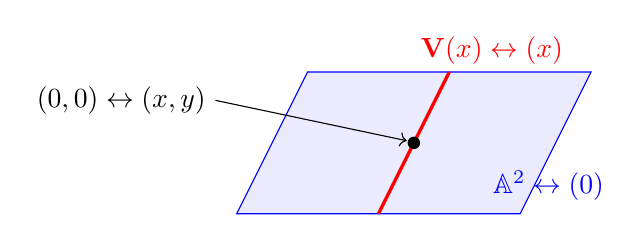
\begin{tikzpicture}[scale=0.9]
  \fill[blue!8] (0,0)--(4,0)--(5,2)--(1,2)--cycle;
  \draw[blue] (0,0)--(4,0)--(5,2)--(1,2)--cycle;
  \draw[very thick,red] (2,0)--(3,2);
  \fill (2.5,1) circle (2.5pt);
  \node[blue] at (4.4,0.4) {$\A^2\leftrightarrow(0)$};
  \node[red] at (3.6,2.3) {$\Zero(x)\leftrightarrow(x)$};
  \node[left] at (-0.3,1.6) {$(0,0)\leftrightarrow(x,y)$};
  \draw[->] (-0.3,1.6)--(2.4,1.03);
\end{tikzpicture}
\caption{素イデアルの鎖 $(0)\subsetneq(x)\subsetneq(x,y)$ と図形の列 $\A^2\supsetneq\text{直線}\supsetneq\text{点}$．包含の向きが逆転する．}
\label{fig:ch02-chain}
\end{figure}

単項イデアル整域では状況が単純である．

\begin{myprop}{PID の素イデアル}{ch02-pid-prime}
$R$ を単項イデアル整域とする．$0$ でない素イデアルは極大イデアルである．
\end{myprop}

\begin{proof}
$\p=(p)\ne0$ を素イデアルとし，$\p\subset(a)$ とする．$p=ab$ と書け，$p\mid a$ または $p\mid b$ である．
$p\mid a$ ならば $(a)=(p)$．$p\mid b$ ならば $b=pc$ と書け，$p=apc$ から（$R$ は整域で $p\ne0$）$ac=1$，すなわち $(a)=R$．
\end{proof}

したがって $\Z$ や $k[x]$ の素イデアルは，$(0)$ と極大イデアルのみである．
$\Z$ の素イデアル全体を図示すると図\ref{fig:ch02-specz}のようになる．
各素数 $p$ が「点」に対応し，$(0)$ は特定の点に対応しない特別な点（\textbf{生成点}）である．
このように素イデアル全体を空間とみなす考え方が，第12章のスキーム $\Spec R$ である．

\begin{figure}[H]
\centering
\begin{tikzpicture}
  \draw[thick] (0,0)--(9.5,0);
  \foreach \x/\p in {0.5/2,1.5/3,2.5/5,3.5/7,4.5/11,5.5/13,6.5/17}{
    \fill (\x,0) circle (2.5pt); \node[below] at (\x,-0.1) {$(\p)$};}
  \node at (7.6,0.25) {$\cdots$};
  \node[red] at (4.5,1) {$(0)$（生成点）};
  \draw[red,dashed,->] (4.5,0.75)--(4.5,0.1);
\end{tikzpicture}
\caption{$\Z$ の素イデアル全体の模式図．各素数 $p$ が閉点 $(p)$ に，$(0)$ が「直線全体に広がった」生成点に対応する．}
\label{fig:ch02-specz}
\end{figure}

\subsection{整域と素イデアル}

\begin{mythm}{素イデアルと整域}{ch02-prime-domain}
環 $R$ のイデアル $\p$ に対し，$\p$ が素イデアルであることと，剰余環 $R/\p$ が整域であることは同値である．
\end{mythm}

\begin{proof}
$R/\p\ne0\iff\p\ne R$．また $\bar a\bar b=\bar0$ in $R/\p$ $\iff ab\in\p$，$\bar a=\bar0\iff a\in\p$ である．
したがって「$R/\p$ に零因子がない」ことは「$ab\in\p\Rightarrow a\in\p$ または $b\in\p$」と同値である．
\end{proof}

特に，環 $R$ が整域であることと $(0)$ が素イデアルであることは同値である．
この定理は，素イデアルであるかどうかの判定によく使われる．たとえば
$k[x,y]/(y-x^2)\cong k[x]$ は整域なので $(y-x^2)$ は素イデアル（放物線は既約），
$k[x,y]/(xy)$ は $x\cdot y=0$ より整域でないので $(xy)$ は素イデアルでない．

\begin{myprop}{素イデアルの引き戻し}{ch02-prime-pullback}
$\varphi:R\to S$ を環準同型，$\q$ を $S$ の素イデアルとすると，$\varphi^{-1}(\q)$ は $R$ の素イデアルである．
\end{myprop}

\begin{proof}
$\varphi^{-1}(\q)$ がイデアルであることは容易．$\varphi(1)=1\notin\q$ より真のイデアル．
$ab\in\varphi^{-1}(\q)$ ならば $\varphi(a)\varphi(b)\in\q$ より $\varphi(a)\in\q$ または $\varphi(b)\in\q$．
（あるいは，$R/\varphi^{-1}(\q)$ が整域 $S/\q$ の部分環と同型であることからも従う．）
\end{proof}

これに対し，極大イデアルの引き戻しは極大とは限らない．包含 $\Z\hookrightarrow\Q$ において，$\Q$ の極大イデアル $(0)$ の引き戻しは
$\Z$ の $(0)$ であり，極大でない．この非対称性が，スキーム論で「点」として素イデアル全体を採用する理由の一つである（第12章）．
ただし，体 $k$ 上有限生成な $k$ 代数の間の $k$ 代数準同型については，極大イデアルの引き戻しは極大イデアルになる
（零点定理の帰結，第4章）．これが「多様体の射は点を点に写す」ことに対応する．

\subsection{体と極大イデアル}

\begin{mythm}{極大イデアルと体}{ch02-max-field}
環 $R$ のイデアル $\m$ に対し，$\m$ が極大イデアルであることと，剰余環 $R/\m$ が体であることは同値である．
\end{mythm}

\begin{proof}
2.5.2小節の対応定理により，$R/\m$ のイデアルは $\m$ を含む $R$ のイデアルと一対一に対応する．
$\m$ が極大 $\iff$ $\m$ を含むイデアルが $\m$ と $R$ のみ $\iff$ $R/\m$ のイデアルが $0$ と $R/\m$ のみ（かつ $R/\m\ne0$）
$\iff$ $R/\m$ は体（命題\ref{prop:ch02-unit-ideal}）．

直接的な証明も与えておく．$\m$ が極大で $a\notin\m$ とすると，$\m+(a)=R$ より $1=m+ra$ と書け，$\bar r\bar a=\bar1$ となる．
逆に $R/\m$ が体で $\m\subsetneq I$ とすると，$a\in I\setminus\m$ に対し $\bar a$ は可逆なので $ra-1\in\m\subset I$，よって $1\in I$．
\end{proof}

体は整域なので，この定理と定理\ref{thm:ch02-prime-domain}から命題\ref{prop:ch02-max-prime}が再び得られる．

\begin{myex}{剰余体の例}{ch02-residue-fields}
(1) $\Z/p\Z=\F_p$ は体．よって $(p)$ は極大．

(2) $k[x_1,\dots,x_n]/\m_a\cong k$．点 $a$ に対応する極大イデアルの剰余体は $k$ そのものであり，
これは「関数 $f$ の点 $a$ での値 $f(a)\in k$」を与える．

(3) $\R[x]/(x^2+1)\cong\C$．剰余体が $\R$ より大きいことが，この極大イデアルが「実の点」ではないことを表している．

(4) $\Q[x]/(x^2-2)\cong\Q(\sqrt2)$．一般に $k[x]/(f)$ は，$f$ が既約なとき体であり（$k[x]$ はPIDなので $(f)$ は極大），
これが $f$ の根を $k$ に添加した体である（Kronecker の構成）．
\end{myex}

$k$ が代数閉体（$k=\C$ など）の場合には，$k[x_1,\dots,x_n]$ の極大イデアルは\emph{すべて} $\m_a$（$a\in k^n$）の形をしている．
これが Hilbert の零点定理の一つの形であり（第4章），
\[
  \A^n_k\text{ の点}\ \longleftrightarrow\ k[x_1,\dots,x_n]\text{ の極大イデアル}
\]
という代数幾何学の最も基本的な対応を与える．$k=\R$ では例(3)のように点に対応しない極大イデアルが存在し，この対応は成り立たない．

\exprob{prob:ch02-4-1}
$\Z[x]$ において $(x)$，$(2,x)$，$(4,x)$ のそれぞれについて，素イデアルか，極大イデアルかを判定せよ．

\exprob{prob:ch02-4-2}
$\R[x,y]$ のイデアル $(x^2+1,\ y)$ は極大イデアルであることを示し，剰余体を求めよ．
またこのイデアルが $\R^2$ のどの点の $\m_a$ とも一致しないことを確かめよ．

%======================================================================
\section{剰余環}
%======================================================================

\subsection{剰余環の構成}

$R$ を環，$I$ をそのイデアルとする．$R$ 上の関係 $\sim$ を
\[
  a\sim b\ \iff\ a-b\in I
\]
で定めると，これは同値関係である（反射律 $0\in I$，対称律 $-x\in I$，推移律 $x+y\in I$ による）．
$a$ の同値類は $a+I=\{a+x\mid x\in I\}$ であり，これを $a$ の $I$ を法とする\textbf{剰余類}といい，$\bar a$ とも書く．
剰余類全体の集合（商集合）を $R/I$ と書く（商集合については付録Aも参照）．

\begin{myprop}{剰余環}{ch02-quotient}
$R/I$ において
\[
  \bar a+\bar b=\overline{a+b},\qquad \bar a\cdot\bar b=\overline{ab}
\]
と定めると，これらは代表元の取り方によらずに定まり，$R/I$ は $\bar0$ を零元，$\bar1$ を単位元とする環になる．
これを $R$ の $I$ による\textbf{剰余環}（商環）という．
自然な射影 $\pi:R\to R/I$，$a\mapsto\bar a$ は全射環準同型で，$\Ker\pi=I$ である．
\end{myprop}

\begin{proof}
$a\sim a'$，$b\sim b'$ とし，$a'=a+x$，$b'=b+y$（$x,y\in I$）と書く．
和については $a'+b'=(a+b)+(x+y)$ で $x+y\in I$．積については
\[
  a'b'=ab+(ay+xb+xy)
\]
であり，イデアルの吸収性から $ay,xb,xy\in I$ なので $a'b'\sim ab$．
環の公理は $R$ の公理から代表元ごとに従う．残りの主張は明らかである．
\end{proof}

この証明で\emph{吸収性}（$I$ の元に任意の元を掛けても $I$ に入る）が積の well-definedness にちょうど必要であることに注意しよう．
単なる部分環や加法部分群で割っても環にはならない．これがイデアルという概念を考える最大の理由である．

剰余環 $R/I$ は「$I$ の元をすべて $0$ とみなす」ことで得られる環である．
たとえば $k[x,y]/(f)$ では関係式 $f=0$ を課して計算する．
幾何学的には，$I=\Ideal(X)$ のとき $k[x_1,\dots,x_n]/I$ は図形 $X$ 上の多項式関数の環（座標環 $k[X]$）である：
2つの多項式が $X$ 上で同じ関数を定めることと，その差が $\Ideal(X)$ に属することは同値だからである（第4章，第5章）．

\begin{myex}{剰余環の例}{ch02-quotient-ex}
(1) $\Z/n\Z$：整数の $n$ を法とする計算．

(2) $\R[x]/(x^2+1)$：任意の多項式は $x^2+1$ で割った余り $a+bx$ と合同であり，$\bar x^2=-1$ を満たす．
$a+b\bar x\mapsto a+bi$ によって $\R[x]/(x^2+1)\cong\C$ となる（$\R[x]\to\C$，$x\mapsto i$ の核が $(x^2+1)$ であることから準同型定理で従う）．
複素数とは「実数に $x^2+1=0$ という関係式を満たす元を付け加えたもの」に他ならない．

(3) $k[x]/(x^2)=k[\varepsilon]$：双対数の環（2.1.5小節）．
\end{myex}

\subsection{商環の普遍性}

\begin{mythm}{剰余環の普遍性}{ch02-quotient-universal}
$I$ を環 $R$ のイデアル，$\pi:R\to R/I$ を自然な射影とする．
環準同型 $\varphi:R\to S$ が $I\subset\Ker\varphi$ を満たすならば，$\varphi=\bar\varphi\circ\pi$ を満たす環準同型
$\bar\varphi:R/I\to S$ がただ一つ存在する．
\[
\begin{tikzcd}
  R \arrow[r,"\varphi"] \arrow[d,"\pi"'] & S\\
  R/I \arrow[ru,dashed,"\exists!\,\bar\varphi"'] &
\end{tikzcd}
\]
\end{mythm}

\begin{proof}
$\bar\varphi(\bar a)=\varphi(a)$ と定める．$\bar a=\bar a'$ ならば $a-a'\in I\subset\Ker\varphi$ より $\varphi(a)=\varphi(a')$ なので well-defined．
準同型性は $\varphi$ から従う．$\pi$ は全射なので，$\bar\varphi\circ\pi=\varphi$ を満たす写像は $\bar\varphi$ しかない．
\end{proof}

この普遍性は，「$R/I$ からの準同型を作ることは，$I$ を $0$ に写す $R$ からの準同型を作ることと同じ」と言い表せる．
多項式環の普遍性（命題\ref{prop:ch02-poly-universal}）と組み合わせると，次のきわめて有用な原理が得られる：
\[
  \Hom_{k\text{-alg}}\big(k[x_1,\dots,x_n]/(f_1,\dots,f_m),\ A\big)
  \ \cong\ \{a\in A^n\mid f_1(a)=\dots=f_m(a)=0\}.
\]
すなわち，$k$ 代数 $k[x]/(f)$ から $A$ への準同型は，方程式系 $f=0$ の $A$ における解と一対一に対応する．
$A=k$ ならば $k$ 上の点（通常の解），$A=\C$（$k=\R$）ならば複素解，$A=k[\varepsilon]$ ならば「無限小だけずれた解」（接ベクトル）が得られる．
これは第12章で「スキームの $A$ 値点」という考え方に発展する．

\begin{mythm}{対応定理}{ch02-correspondence}
$I$ を環 $R$ のイデアルとし，$\pi:R\to R/I$ を自然な射影とする．このとき
\[
  \{R\text{ のイデアル }J\text{ で }J\supset I\}\ \longleftrightarrow\ \{R/I\text{ のイデアル}\},\qquad J\mapsto J/I=\pi(J)
\]
は包含関係を保つ一対一対応であり，逆写像は $\bar J\mapsto\pi^{-1}(\bar J)$ で与えられる．さらにこの対応で，素イデアルは素イデアルに，極大イデアルは極大イデアルに対応する．
\end{mythm}

\begin{proof}
$\pi$ が全射であることから $\pi(\pi^{-1}(\bar J))=\bar J$．また $J\supset I=\Ker\pi$ ならば $\pi^{-1}(\pi(J))=J+I=J$．
$\pi(J)$ がイデアルであることも $\pi$ の全射性から従う．包含関係の保存は明らか．
素・極大については，第三同型定理 $(R/I)/(J/I)\cong R/J$ と定理\ref{thm:ch02-prime-domain}，定理\ref{thm:ch02-max-field}から従う．
\end{proof}

幾何学的には，$R/I$ のイデアル（$=$ 図形 $\Zero(I)$ の部分図形）は，$I$ を含む $R$ のイデアル（$=$ 全体空間の部分図形で $\Zero(I)$ に含まれるもの）
と同じである，ということを表している．たとえば $\Z/12\Z$ のイデアルは，図\ref{fig:ch02-hasse}の6個に対応する．

\subsection{剰余環の零因子}

剰余環 $R/I$ の零因子や冪零元は，$I$ の性質を反映する．
定理\ref{thm:ch02-prime-domain}により，$R/I$ が零因子をもたないのは $I$ が素イデアルのときに限る．
冪零元については次の概念が重要である．

\begin{mydef}{根基と被約環}{ch02-radical}
イデアル $I$ に対し，
\[
  \sqrt{I}=\{a\in R\mid \text{ある }m\ge1\text{ に対し }a^m\in I\}
\]
を $I$ の\textbf{根基}という．$\sqrt I=I$ となるイデアルを\textbf{根基イデアル}という．
冪零元が $0$ しかない環を\textbf{被約環}という．
\end{mydef}

$\sqrt I$ はイデアルである（$a^m,b^n\in I$ ならば二項展開により $(a+b)^{m+n-1}\in I$）．
定義から，$R/I$ の冪零元はちょうど $\sqrt I/I$ の元であり，したがって
\[
  R/I\ \text{が被約}\iff I=\sqrt I.
\]
素イデアルは根基イデアルである（$a^m\in\p\Rightarrow a\in\p$）．根基イデアルは第4章で中心的な役割を果たす．

\begin{myex}{零因子と冪零元の幾何学}{ch02-zerodiv-geom}
(1) $R=k[x,y]/(xy)$（2本の座標軸の和集合の関数環）．$\bar x\bar y=0$ であり，$\bar x,\bar y$ は零因子である．
$\bar x$ は $y$軸上で $0$，$\bar y$ は $x$軸上で $0$ となる関数であり，「それぞれ別の成分上でのみ $0$ でない関数の積は $0$」という状況である．
$(xy)$ は根基イデアルなので $R$ は被約である．

(2) $R=k[x]/(x^2)$．$\bar x\ne0$ だが $\bar x^2=0$．零点集合 $\Zero(x^2)$ は原点1点であるが，
$R$ は「原点の値 $f(0)$」と「原点での微分 $f'(0)$」の情報を保持している（$f\equiv f(0)+f'(0)x\pmod{x^2}$）．
このため $\Zero(x^2)$ を\textbf{二重点}あるいは「接ベクトル方向に太った点」とみなす（図\ref{fig:ch02-double-point}，第12章）．

(3) $\Z/12\Z$：零因子は $\bar2,\bar3,\bar4,\bar6,\bar8,\bar9,\bar{10}$，冪零元は $\bar0,\bar6$ である．
$\sqrt{(12)}=(6)$ であり，$12=2^2\cdot3$ の「$2$ の重複」が冪零元 $\bar6$ として現れている．
\end{myex}

\begin{figure}[H]
\centering
\begin{tikzpicture}
  \begin{scope}
    \draw[->,gray] (-1.5,0)--(1.5,0) node[right]{$x$};
    \fill[blue] (0,0) circle (2.5pt);
    \node at (0,-0.7) {$k[x]/(x)\cong k$：単純な点};
  \end{scope}
  \begin{scope}[xshift=5.5cm]
    \draw[->,gray] (-1.5,0)--(1.5,0) node[right]{$x$};
    \fill[blue] (0,0) circle (2.5pt);
    \draw[->,very thick,blue] (0,0)--(0.7,0);
    \node at (0,-0.7) {$k[x]/(x^2)$：二重点（接方向の情報をもつ）};
  \end{scope}
\end{tikzpicture}
\caption{被約な点と二重点．どちらも零点集合は原点1点だが，関数環が異なる．}
\label{fig:ch02-double-point}
\end{figure}

\subsection{剰余環と多項式方程式}

剰余環は，多項式方程式を「解かずに」調べる道具である．一変数の場合から始めよう．

\begin{myprop}{$k[x]/(f)$ の構造}{ch02-kx-mod-f}
$f\in k[x]$ を次数 $d\ge1$ の多項式とすると，$k[x]/(f)$ は $\bar1,\bar x,\dots,\bar x^{d-1}$ を基底とする $d$ 次元 $k$ ベクトル空間である．
さらに $k$ が代数閉体で $f=c\prod_{i=1}^r(x-a_i)^{e_i}$（$a_i$ は相異なる）と因数分解されるならば
\[
  k[x]/(f)\ \cong\ \prod_{i=1}^rk[x]/\big((x-a_i)^{e_i}\big)
\]
であり，$\dim_kk[x]/((x-a_i)^{e_i})=e_i$ である．
\end{myprop}

\begin{proof}
割り算の原理により，任意の $g$ は $f$ による余り（次数 $<d$）と合同であり，次数 $<d$ の2つの多項式が合同なら差は $f$ の倍数で次数 $<d$ なので $0$ である．
後半は，$(x-a_i)^{e_i}$ たちが互いに素である（$i\ne j$ について $(x-a_i)^{e_i}$ と $(x-a_j)^{e_j}$ の生成するイデアルは，
$k[x]$ がPIDで両者に共通因子がないので $(1)$）ことから，中国剰余定理を繰り返し用いればよい．
\end{proof}

この命題は「$\dim_kk[x]/(f)=\deg f=$ 重複度込みの根の個数」を意味し，さらに各根の重複度 $e_i$ が局所的な因子の次元として捉えられることを示している．
重根がなければ $k[x]/(f)\cong k^d$（$d$ 個の点上の関数環）であり，重根があれば冪零元が現れる．

この考え方は多変数にもそのまま拡張される．第1章1.1.3小節の円と直線の交点を，剰余環で見直してみよう．
簡単のため放物線 $y=x^2$ と直線 $y=c$ の交わりを考えると，
\[
  k[x,y]/(y-x^2,\ y-c)\ \cong\ k[x]/(x^2-c)
\]
である（$y$ を $c$ に置き換える）．$c\ne0$（$k=\C$）ならばこれは $k\times k$ と同型で2点を表し，
$c=0$ ならば $k[x]/(x^2)$ となって冪零元をもつ．直線 $y=0$ が放物線に\emph{接する}ことが，剰余環の冪零元として正確に捉えられている．
交点の重複度を剰余環の次元として定義することは，第9章で Bézout の定理を述べる際の基礎となる．

\begin{physbox}[カイラル環とWitten指数]
2次元の $\mathcal N=(2,2)$ Landau--Ginzburg 模型は，超ポテンシャル $W(x_1,\dots,x_n)$（多項式）で定まる．
その\textbf{カイラル環}は剰余環
\[
  \C[x_1,\dots,x_n]\big/\big(\partial W/\partial x_1,\dots,\partial W/\partial x_n\big)
\]
で与えられ（Jacobi環），臨界点が孤立している場合，その $\C$ 上の次元が真空の数（Witten指数）に等しい．
たとえば $W=x^{n+1}/(n+1)$ ならば $W'=x^n$ で，カイラル環は $\C[x]/(x^n)$，次元は $n$ である．
$W$ を変形して $W'=x^n-\varepsilon$（$\varepsilon\ne0$）とすると，臨界点は $n$ 個の相異なる点に分かれ，カイラル環は $\C^n$ と同型になる．
次元（真空の数）は変形で保たれ，縮退した真空が分裂する様子は，命題\ref{prop:ch02-kx-mod-f}の重根の分離そのものである．
\end{physbox}

\exprob{prob:ch02-5-1}
$\Q[x]/(x^3-2)$ が体であることを示し，その中で $\overline{1+x}$ の逆元を $a+b\bar x+c\bar x^2$（$a,b,c\in\Q$）の形で求めよ．

\exprob{prob:ch02-5-2}
$k=\C$ とする．$\C[x,y]/(x^2+y^2-1,\ y-c)$ の $\C$ 上の次元を求め，それが冪零元をもつような $c$ の値をすべて求めよ．
その値は第1章1.1.3小節の接線条件とどう関係するか．

%======================================================================
\section{多項式環}
%======================================================================

\subsection{一変数多項式環}

$R$ を環とする．$R$ 係数の一変数多項式 $f=a_nx^n+\dots+a_1x+a_0$（$a_n\ne0$）に対し，$n$ を\textbf{次数}，$a_n$ を\textbf{最高次係数}という．
$a_n=1$ のとき $f$ を\textbf{モニック}という．零多項式の次数は $-\infty$ と約束する．

\begin{myprop}{次数の性質}{ch02-degree}
$R$ が整域ならば，$f,g\in R[x]$ に対して $\deg(fg)=\deg f+\deg g$ が成り立つ．
したがって $R[x]$ は整域であり，$R[x]^\times=R^\times$ である．
\end{myprop}

\begin{proof}
$f,g\ne0$ の最高次係数を $a,b$ とすると，$fg$ の $x^{\deg f+\deg g}$ の係数は $ab\ne0$（整域）．
可逆元について：$fg=1$ ならば $\deg f+\deg g=0$ より $f,g\in R$ であり，$f\in R^\times$．
\end{proof}

整域でない場合，たとえば $(\Z/4\Z)[x]$ では $(1+2x)^2=1+4x+4x^2=1$ であり，次数 $1$ の多項式が可逆になる．

\begin{mythm}{割り算の原理}{ch02-division}
$R$ を環，$g\in R[x]$ を最高次係数が可逆な多項式（たとえばモニック）とする．
任意の $f\in R[x]$ に対して，
\[
  f=qg+r,\qquad \deg r<\deg g
\]
を満たす $q,r\in R[x]$ が一意に存在する．
\end{mythm}

\begin{proof}
存在：$\deg f$ に関する帰納法．$\deg f<\deg g$ なら $q=0$，$r=f$．$\deg f=n\ge m=\deg g$ のとき，
$f$ の最高次係数を $a$，$g$ の最高次係数を $b$ として $f_1=f-ab^{-1}x^{n-m}g$ とおくと $\deg f_1<n$ であり，
帰納法の仮定から $f_1=q_1g+r$ と書けるので $f=(q_1+ab^{-1}x^{n-m})g+r$．
一意性：$qg+r=q'g+r'$ ならば $(q-q')g=r'-r$．$q\ne q'$ ならば左辺の次数は $\ge\deg g$（$g$ の最高次係数が可逆なので零因子でない）
だが右辺の次数は $<\deg g$ で矛盾．
\end{proof}

例\ref{ex:ch02-parabola}や例\ref{ex:ch02-cusp}では，$R=k[x]$ 上の $y$ の多項式として，モニックな $y-x^2$ や $y^2-x^3$ で割る操作を行った．
最高次係数が可逆であれば，係数環が体でなくても割り算ができることが要点である．

\begin{mycor}{因数定理と根の個数}{ch02-factor-thm}
$R$ を環，$f\in R[x]$，$a\in R$ とする．
\begin{enumerate}
  \item $f(a)=0\iff(x-a)\mid f$．
  \item $R$ が整域で $f\ne0$ ならば，$f$ の $R$ における根の個数は $\deg f$ 以下である．
\end{enumerate}
\end{mycor}

\begin{proof}
(1) $x-a$ で割ると $f=q\cdot(x-a)+r$，$r\in R$．$x=a$ を代入して $r=f(a)$．
(2) $\deg f$ に関する帰納法．根 $a$ があれば $f=(x-a)q$，$\deg q=\deg f-1$．別の根 $b\ne a$ は $(b-a)q(b)=0$ より（整域）$q(b)=0$ を満たすので，
$f$ の根は $a$ と $q$ の根のみである．
\end{proof}

$R$ が整域でないと (2) は成り立たない．$\Z/8\Z$ において $x^2-1$ は $\bar1,\bar3,\bar5,\bar7$ の4個の根をもつ．

体 $k$ 上の $k[x]$ はPIDであった（定理\ref{thm:ch02-pid}）．Euclidの互除法により，$f,g$ の最大公約元 $d=\gcd(f,g)$ が計算でき，
$d=af+bg$ となる $a,b\in k[x]$ が存在する（$(f)+(g)=(d)$）．

\subsection{多変数多項式環}

多変数多項式環は，一変数多項式環を繰り返して作ることができる：
\[
  R[x_1,\dots,x_n]\cong R[x_1,\dots,x_{n-1}][x_n].
\]
すなわち $n$ 変数多項式は，$x_n$ についての多項式で，係数が $x_1,\dots,x_{n-1}$ の多項式であるものとみなせる．
この見方は，帰納法による証明（命題\ref{prop:ch02-domain-poly}，定理\ref{thm:ch02-hilbert-basis}など）で頻繁に用いられる．

$f=\sum c_\alpha x^\alpha$ に対し，次数 $d$ の単項式の部分 $f_d=\sum_{|\alpha|=d}c_\alpha x^\alpha$ を $f$ の\textbf{$d$次斉次成分}という．
$f=f_0+f_1+\dots+f_m$ と一意に分解される．すべての項が同じ次数 $d$ をもつ多項式を\textbf{$d$次斉次多項式}という．
$d$ 次斉次多項式全体を $S_d$ と書くと，
\[
  k[x_1,\dots,x_n]=\bigoplus_{d\ge0}S_d,\qquad S_dS_e\subset S_{d+e},\qquad \dim_kS_d=\binom{n+d-1}{d}
\]
が成り立つ．このような構造をもつ環を\textbf{次数付き環}という．斉次多項式は射影空間 $\PP^{n-1}$ 上の図形を定義するのに用いられる（第8章）．

多変数の場合，一変数の割り算の原理はそのままでは成り立たない．たとえば $x$ と $y$ のどちらで先に割るかによって余りが変わる．
単項式に適切な順序（\textbf{単項式順序}，たとえば辞書式順序）を固定すると，多変数の割り算アルゴリズムが定義でき，
さらに余りが一意に定まるような生成系として\textbf{Gröbner基底}が定義される．
Gröbner基底は，連立多項式方程式の消去や，イデアルの所属判定を計算機で行うための基本的な道具であるが，本ノートでは深入りしない．

\subsection{多項式環の代数的構造}

\begin{myprop}{多項式環は整域}{ch02-domain-poly}
$R$ が整域ならば $R[x_1,\dots,x_n]$ は整域であり，$R[x_1,\dots,x_n]^\times=R^\times$ である．
特に体 $k$ 上の多項式環 $k[x_1,\dots,x_n]$ は整域で，可逆元は $0$ でない定数のみである．
\end{myprop}

\begin{proof}
$n$ に関する帰納法と，$R[x_1,\dots,x_n]=R[x_1,\dots,x_{n-1}][x_n]$ に命題\ref{prop:ch02-degree}を適用すればよい．
\end{proof}

幾何学的には，$k[x_1,\dots,x_n]$ が整域であることは「アフィン空間 $\A^n$ は既約である」ことに対応する（第3章）．
また，可逆元が定数のみであることは，「$\A^n$ 上どこでも $0$ にならない多項式関数は定数のみ」であることを意味する
（$k$ が代数閉体のとき．命題\ref{prop:ch01-complex-nonempty}を参照）．

\begin{mydef}{有限生成代数}{ch02-fg-algebra}
$k$ を体とする．環 $A$ と環準同型 $k\to A$ の組を\textbf{$k$代数}という．
ある $a_1,\dots,a_n\in A$ によって $A=k[a_1,\dots,a_n]$（$a_i$ の $k$ 係数多項式全体）となるとき，$A$ を\textbf{有限生成 $k$ 代数}という．
\end{mydef}

\begin{myprop}{有限生成代数は多項式環の剰余環}{ch02-fg-quotient}
$A$ が $a_1,\dots,a_n$ で生成される $k$ 代数ならば，あるイデアル $I\subset k[x_1,\dots,x_n]$ によって $A\cong k[x_1,\dots,x_n]/I$ となる．
\end{myprop}

\begin{proof}
多項式環の普遍性により $\varphi:k[x_1,\dots,x_n]\to A$，$x_i\mapsto a_i$ が定まり，生成の仮定から全射である．
準同型定理より $A\cong k[x_1,\dots,x_n]/\Ker\varphi$．
\end{proof}

この命題により，有限生成 $k$ 代数は「$\A^n$ の中の方程式系 $I$ で定まる図形の関数環」と考えることができる．
アフィン代数幾何学（第5章）の対象である座標環は，すべて被約な有限生成 $k$ 代数である．

\subsection{多項式の因数分解}

整数が素数の積に一意的に分解されるように，多項式も既約多項式の積に分解される．これを一般の整域で定式化しよう．

\begin{mydef}{既約元・素元・UFD}{ch02-ufd}
$R$ を整域とし，$a\in R$ を $0$ でも可逆でもない元とする．
\begin{enumerate}
  \item $a=bc$ ならば $b$ か $c$ が可逆であるとき，$a$ を\textbf{既約元}という．
  \item $a\mid bc$ ならば $a\mid b$ または $a\mid c$ であるとき，すなわち $(a)$ が素イデアルのとき，$a$ を\textbf{素元}という．
\end{enumerate}
$0$ でも可逆でもないすべての元が既約元の積に表され，その表し方が順序と同伴を除いて一意であるとき，$R$ を\textbf{一意分解整域}（UFD）という．
\end{mydef}

整域において素元は既約元である（$a=bc$ ならば $a\mid b$ または $a\mid c$；$a\mid b$ なら $b=ad$ から $a=adc$，$dc=1$ で $c$ は可逆）．
逆は一般には成り立たないが，UFDでは既約元は素元である．

\begin{myex}{一意分解が成り立たない例}{ch02-non-ufd}
$R=\Z[\sqrt{-5}]$ において
\[
  6=2\cdot3=(1+\sqrt{-5})(1-\sqrt{-5}).
\]
ノルム $N(a+b\sqrt{-5})=a^2+5b^2$ は乗法的で，$N(u)=1$ と $u$ が可逆であることは同値である．
$N(2)=4$，$N(3)=9$，$N(1\pm\sqrt{-5})=6$ であり，ノルムが $2$ や $3$ になる元は存在しない（$a^2+5b^2=2,3$ は整数解をもたない）ので，
これら4つの元はすべて既約である．また $2$ と $1\pm\sqrt{-5}$ はノルムが異なるので同伴でない．
したがって $6$ は本質的に異なる2通りの既約分解をもち，$R$ はUFDではない．特に既約元 $2$ は素元でない．
\end{myex}

\begin{mythm}{一意分解整域の基本定理}{ch02-ufd-thms}
\begin{enumerate}
  \item 単項イデアル整域はUFDである．特に $\Z$ と $k[x]$ はUFDである．
  \item （Gauss）$R$ がUFDならば $R[x]$ もUFDである．
  \item 特に，体 $k$ 上の多項式環 $k[x_1,\dots,x_n]$ および $\Z[x_1,\dots,x_n]$ はUFDである．
\end{enumerate}
\end{mythm}

\begin{proof}[証明の概略]
(1) 既約分解の存在は，分解が無限に続くと単項イデアルの真の昇鎖 $(a_1)\subsetneq(a_2)\subsetneq\cdots$ が得られ，
PIDがNoether環であること（2.7節）に矛盾することから従う．一意性は，PIDでは既約元 $p$ に対し $(p)$ が極大イデアル，したがって素イデアルであることを用いて，
整数の場合と同様に示される．

(2) $K=\Frac R$ とする．多項式 $f\in R[x]$ の係数の最大公約元を\textbf{内容} $c(f)$ と呼び，$c(f)$ が可逆なとき $f$ を\textbf{原始的}という．
鍵となるのは\textbf{Gaussの補題}「原始多項式の積は原始的である」である（素元 $p$ に対し，$(R/p)[x]$ が整域であることから従う）．
これにより，$R[x]$ の元の分解は「内容の $R$ における分解」と「$K[x]$（PIDなのでUFD）における分解」に帰着される．

(3) (1)(2)と $n$ に関する帰納法による．
\end{proof}

UFDの幾何学的な意味は次の通りである．$k[x_1,\dots,x_n]$ の $0$ でない非可逆元 $f$ を既約分解して $f=c\,f_1^{e_1}\cdots f_r^{e_r}$ とすると，
\[
  \Zero(f)=\Zero(f_1)\cup\dots\cup\Zero(f_r),\qquad \sqrt{(f)}=(f_1f_2\cdots f_r)
\]
であり，各 $(f_i)$ は素イデアル（$f_i$ は素元）であるから $\Zero(f_i)$ は既約な超曲面である．
つまり\emph{超曲面の既約成分への分解は，定義多項式の因数分解で与えられる}（第3章）．
UFDでは「余次元1の既約図形は1つの方程式で定義される」ことも成り立ち，これは第15章などで因子（divisor）を扱う際の基礎となる．

\subsection{既約多項式}

体 $k$ 上の多項式 $f\in k[x]$ が既約であるかどうかは，体 $k$ に強く依存する．
\begin{itemize}
  \item 一次式は常に既約である．
  \item 次数 $2,3$ の多項式が既約であることと，$k$ に根をもたないことは同値である（分解すれば一次因子をもつため）．
  \item $k=\C$（代数閉体）では，既約多項式は一次式のみである（代数学の基本定理）．
  \item $k=\R$ では，既約多項式は一次式と，判別式が負の二次式のみである（複素根は共役な組で現れるため）．
  \item $k=\Q$ では，任意の次数の既約多項式が存在する（たとえば $x^n-2$．下の Eisenstein の判定法による）．
\end{itemize}

\begin{mythm}{Eisensteinの判定法}{ch02-eisenstein}
$R$ を整域，$p\in R$ を素元とし，
\[
  f=a_nx^n+a_{n-1}x^{n-1}+\dots+a_0\in R[x]\qquad(n\ge1)
\]
が次を満たすとする：
\[
  p\nmid a_n,\qquad p\mid a_i\ (0\le i\le n-1),\qquad p^2\nmid a_0.
\]
このとき $f$ は，次数1以上の2つの多項式の積 $f=gh$（$g,h\in R[x]$）に分解しない．
特に $f$ がモニックならば $f$ は $R[x]$ の既約元である．
さらに $R$ がUFDならば，$f$ は $\Frac(R)[x]$ においても既約である．
\end{mythm}

\begin{proof}
$f=gh$，$g=b_rx^r+\dots+b_0$，$h=c_sx^s+\dots+c_0$，$r,s\ge1$，$r+s=n$ と仮定する．
$\bar R=R/(p)$ は整域であり，$\bar R[x]$ において $\bar f=\bar a_nx^n$（$\bar a_n\ne0$）となる．
$\bar b_r\bar c_s=\bar a_n\ne0$ より $\deg\bar g=r$，$\deg\bar h=s$．
$\bar g,\bar h$ の最低次の $0$ でない項をそれぞれ $\bar b_ix^i$，$\bar c_jx^j$ とすると，$\bar R$ が整域であるから
$\bar g\bar h$ の最低次の項は $\bar b_i\bar c_jx^{i+j}\ne0$ であり，これが $\bar a_nx^n$ に等しいので $i+j=n$．
$i\le r$，$j\le s$，$r+s=n$ より $i=r$，$j=s$，すなわち $\bar g=\bar b_rx^r$，$\bar h=\bar c_sx^s$ である．
$r,s\ge1$ より $p\mid b_0$ かつ $p\mid c_0$ となり，$p^2\mid b_0c_0=a_0$ が従って矛盾する．
$f$ がモニックなら，次数 $0$ の因子 $c\in R$ は最高次係数 $1$ を割るので可逆であり，$f$ は既約元である．
最後の主張は Gauss の補題（定理\ref{thm:ch02-ufd-thms}の証明参照）により，$\Frac(R)[x]$ での分解が $R[x]$ での分解に持ち上がることから従う．
\end{proof}

\begin{myex}{Eisensteinの判定法の応用}{ch02-eisenstein-ex}
(1) $x^n-2\in\Q[x]$ は $p=2$ について Eisenstein 条件を満たすので，任意の $n\ge1$ について既約である．

(2) 素数 $p$ に対し，円分多項式 $\Phi_p(x)=x^{p-1}+x^{p-2}+\dots+1=\dfrac{x^p-1}{x-1}$ は $\Q$ 上既約である．
実際 $x=y+1$ と置換すると $\Phi_p(y+1)=\dfrac{(y+1)^p-1}{y}=y^{p-1}+\binom{p}{1}y^{p-2}+\dots+\binom{p}{p-1}$ であり，
二項係数 $\binom pi$（$1\le i\le p-1$）はすべて $p$ で割り切れ，定数項 $\binom{p}{p-1}=p$ は $p^2$ で割り切れない．
（置換 $x\mapsto y+1$ は環の自己同型なので既約性を保つ．）

(3) \textbf{多変数の場合．}$R=k[x]$（UFD）上の $y$ の多項式として考える．$\mathrm{char}\,k\ne2$ とする．
\begin{itemize}
  \item $y^2+(x^2-1)$：$p=x-1$ とすると，$x^2-1=(x-1)(x+1)$ は $p$ で割り切れ $p^2$ では割り切れない．
        よって円 $x^2+y^2-1$ は $k[x,y]$ で既約である（$y$ についてモニック）．
  \item $y^2-x^3$：$p=x$ について $p\mid x^3$，$p^2\nmid x^3$ は成り立たない（$x^2\mid x^3$）．
        そこで $x$ と $y$ の役割を入れ替え，$R=k[y]$ 上の $x$ の多項式 $-(x^3-y^2)$ と見て $p=y$ を用いると，$y\mid y^2$ だが $y^2\mid y^2$ なのでこれも失敗する．
        この場合は直接示すのがよい：$y^2-x^3$ が分解すれば，$y$ についてモニックな二次式なので $(y-a(x))(y+a(x))$ の形（$y$ の一次の係数が $0$ だから）
        となり $a(x)^2=x^3$ を得るが，左辺の次数は偶数，右辺は奇数で矛盾．
  \item $y^2-(x^3-x)$：$p=x$ とすると $x^3-x=x(x-1)(x+1)$ は $x$ で割り切れ $x^2$ では割り切れない．
        よって第1章の楕円曲線 $y^2=x^3-x$ の定義多項式は既約である．
\end{itemize}
なお，既約性は体に依存する：$x^2+y^2$ は $\R[x,y]$ で既約（Eisenstein を $p=x$ に用いることはできないが，一次式の積に書けないことは直接確かめられる）
だが，$\C[x,y]$ では $(x+iy)(x-iy)$ と分解する．
\end{myex}

\exprob{prob:ch02-6-1}
$f=x^4+1\in\Q[x]$ は既約であることを，$x\mapsto x+1$ と置換して Eisenstein の判定法を用いて示せ．
また $f$ を $\R[x]$ で既約因子に分解せよ．

\exprob{prob:ch02-6-2}
$k$ を標数 $2$ でない体とする．$x^2+y^2-1$ は $k[x,y]$ で既約であるが，標数 $2$ の体上では既約でないことを示せ．

%======================================================================
\section{Noether性}
%======================================================================

\subsection{昇鎖条件}

\begin{mydef}{昇鎖条件}{ch02-acc}
環 $R$ のイデアルの任意の昇鎖
\[
  I_1\subset I_2\subset I_3\subset\cdots
\]
に対して，ある $N$ が存在して $I_N=I_{N+1}=\cdots$ となる（鎖が\textbf{停留する}）とき，$R$ は\textbf{昇鎖条件}（ACC）を満たすという．
\end{mydef}

\begin{myex}{$\Z$ の昇鎖と降鎖}{ch02-acc-z}
$\Z$ の昇鎖 $(I_i)=(n_i)$ では，$n_{i+1}\mid n_i$ であるから，$|n_i|$（$n_1\ne0$ のとき）は非増加な正整数の列であり，いずれ一定になる．
したがって $\Z$ は昇鎖条件を満たす．たとえば $(24)\subset(12)\subset(6)\subset(3)\subset(1)$ は有限回で止まる．
一方，降鎖 $(2)\supsetneq(4)\supsetneq(8)\supsetneq\cdots$ は停留しない．すなわち $\Z$ は降鎖条件を満たさない．
\end{myex}

昇鎖条件は「イデアルを大きくしていく操作は有限回で終わる」ことを主張している．
幾何学的には，イデアルの昇鎖は図形の降鎖 $\Zero(I_1)\supset\Zero(I_2)\supset\cdots$ に対応するので，
\emph{代数的集合を小さくしていく操作は有限回で止まる}ことになる（2.7.5小節）．

\subsection{Noether環}

\begin{mythm}{Noether環の同値条件}{ch02-noether-equiv}
環 $R$ について，次の3条件は同値である．
\begin{enumerate}
  \item $R$ は昇鎖条件を満たす．
  \item （極大条件）$R$ のイデアルからなる空でない任意の族は，包含関係について極大元をもつ．
  \item $R$ のすべてのイデアルは有限生成である．
\end{enumerate}
これらを満たす環を\textbf{Noether環}という．
\end{mythm}

\begin{proof}
(1)$\Rightarrow$(2)：空でない族 $\Sigma$ が極大元をもたないとすると，任意の $I_1\in\Sigma$ に対し $I_1\subsetneq I_2$ となる $I_2\in\Sigma$ があり，
これを繰り返して（従属選択により）停留しない昇鎖が得られ，(1)に反する．

(2)$\Rightarrow$(3)：イデアル $I$ に含まれる有限生成イデアル全体の族 $\Sigma$（$(0)\in\Sigma$ なので空でない）の極大元 $J$ をとる．
$J\ne I$ ならば $a\in I\setminus J$ に対し $J+(a)\in\Sigma$ は $J$ を真に含み，極大性に反する．よって $I=J$ は有限生成．

(3)$\Rightarrow$(1)：昇鎖 $I_1\subset I_2\subset\cdots$ に対し，$I=\bigcup_iI_i$ はイデアルである（鎖であるから）．
仮定より $I=(a_1,\dots,a_m)$ と書け，各 $a_j$ はある $I_{i_j}$ に属する．$N=\max_ji_j$ とすると $a_1,\dots,a_m\in I_N$ なので
$I\subset I_N\subset I_{N+1}\subset\dots\subset I$，すなわち $n\ge N$ で $I_n=I_N$．
\end{proof}

\begin{myex}{Noether環とそうでない環}{ch02-noether-ex}
(1) 体はNoether環である（イデアルは $0$ と全体のみ）．

(2) 単項イデアル整域（$\Z$，$k[x]$ など）はNoether環である（すべてのイデアルが1元で生成される）．

(3) 無限個の変数をもつ多項式環 $k[x_1,x_2,x_3,\dots]$ はNoether環でない．
昇鎖 $(x_1)\subsetneq(x_1,x_2)\subsetneq(x_1,x_2,x_3)\subsetneq\cdots$ が停留しない．

(4) $\R$ 上の $C^\infty$ 級関数全体の環 $C^\infty(\R)$ はNoether環でない．
$I_n=\{f\mid [-1/n,1/n]\text{ 上で }f=0\}$ とおくと $I_1\subsetneq I_2\subsetneq\cdots$ は停留しない
（$[-1/(n+1),1/(n+1)]$ では消えるが $[-1/n,1/n]$ では消えない $C^\infty$ 関数が，隆起関数を用いて構成できる）．
これは，滑らかな関数では「台」を自由に調節できるのに対し，多項式は局所的な振る舞いで全体が決まってしまう（剛性をもつ）ことの反映である．
\end{myex}

\subsection{Noether環の基本性質}

\begin{myprop}{Noether環の剰余環}{ch02-noether-quotient}
$R$ がNoether環で $I$ がイデアルならば，$R/I$ もNoether環である．
より一般に，Noether環の準同型像はNoether環である．
\end{myprop}

\begin{proof}
対応定理（定理\ref{thm:ch02-correspondence}）により，$R/I$ のイデアルの昇鎖は $I$ を含む $R$ のイデアルの昇鎖に対応し，後者は停留する．
\end{proof}

一方，Noether環の\emph{部分環}はNoether環とは限らない．たとえば $k[x_1,x_2,\dots]$ はNoether環でないが，
その分数体 $k(x_1,x_2,\dots)$ は体なのでNoether環である．

Noether環では次の\textbf{Noether帰納法}が使える：
「イデアル $I$ についての性質 $P(I)$ を示すのに，$I$ より真に大きいすべてのイデアル $J$ について $P(J)$ が成り立つと仮定して $P(I)$ を示せば十分である」．
実際，$P$ が成り立たないイデアルの族が空でないとすると，その極大元 $I$ をとれば，$I$ より大きいイデアルでは $P$ が成り立つので仮定から $P(I)$ も成り立ち，矛盾する．

\begin{myprop}{イデアルは素イデアルの積を含む}{ch02-contains-prime-product}
$R$ をNoether環とする．$R$ の任意のイデアル $I\ne R$ は，$I$ を含む有限個の素イデアルの積を含む．
\end{myprop}

\begin{proof}
Noether帰納法を用いる．$I$ が素イデアルなら明らか．そうでなければ $ab\in I$，$a,b\notin I$ となる $a,b$ がある．
$I+(a)$，$I+(b)$ は $I$ を真に含む．これらが $R$ に等しい場合も含めて考えるため，$R$ は「空の積」を含むと約束すると，
帰納法の仮定より $I+(a)\supset\p_1\cdots\p_r$，$I+(b)\supset\q_1\cdots\q_s$（各素イデアルは $I+(a)$ または $I+(b)$ を，したがって $I$ を含む）．
$(I+(a))(I+(b))\subset I+(ab)=I$ より $\p_1\cdots\p_r\q_1\cdots\q_s\subset I$．
なお $I+(a)=R$ かつ $I+(b)=R$ とすると $R=R\cdot R\subset I$ となって $I\ne R$ に反するので，少なくとも一方は真のイデアルであり，素イデアルの積は空にならない．
\end{proof}

幾何学的には，この命題は「代数的集合 $\Zero(I)$ は有限個の既約な代数的集合 $\Zero(\p_i)$ の和集合に含まれる（実は一致させられる）」ことを意味し，
第3章の既約分解定理の代数的な原型である．

\subsection{Hilbertの基底定理}

\begin{mythm}{Hilbertの基底定理}{ch02-hilbert-basis}
$R$ がNoether環ならば，多項式環 $R[x]$ もNoether環である．
\end{mythm}

\begin{proof}
$I\subset R[x]$ をイデアルとし，$I$ が有限生成でないと仮定して矛盾を導く．
$f_1\in I$ を $I\setminus\{0\}$ の中で次数最小の元とし，帰納的に $f_{k+1}$ を $I\setminus(f_1,\dots,f_k)$ の中で次数最小の元とする
（$I$ は有限生成でないので $I\setminus(f_1,\dots,f_k)\ne\emptyset$）．
$d_k=\deg f_k$，$a_k$ を $f_k$ の最高次係数とする．作り方から $d_1\le d_2\le\cdots$ である
（$f_{k+1}\in I\setminus(f_1,\dots,f_{k-1})$ なので，$f_k$ の選び方の最小性から $d_k\le d_{k+1}$）．

$R$ のイデアルの昇鎖 $(a_1)\subset(a_1,a_2)\subset(a_1,a_2,a_3)\subset\cdots$ は $R$ がNoether環であることから停留するので，
ある $N$ について $a_{N+1}\in(a_1,\dots,a_N)$，すなわち $a_{N+1}=\sum_{i=1}^Nr_ia_i$（$r_i\in R$）と書ける．そこで
\[
  g=f_{N+1}-\sum_{i=1}^Nr_ix^{d_{N+1}-d_i}f_i
\]
とおく（$d_i\le d_{N+1}$ なので $x$ の冪は非負）．右辺の和の各項の $x^{d_{N+1}}$ の係数は $r_ia_i$ であり，その和は $a_{N+1}$ に等しいので，
$g$ の $x^{d_{N+1}}$ の係数は $0$，すなわち $\deg g<d_{N+1}$ である．
また，$g\in(f_1,\dots,f_N)$ ならば $f_{N+1}\in(f_1,\dots,f_N)$ となって $f_{N+1}$ の選び方に反するので，$g\in I\setminus(f_1,\dots,f_N)$．
これは $f_{N+1}$ が $I\setminus(f_1,\dots,f_N)$ の中で次数最小であることに矛盾する．
\end{proof}

\begin{mycor}{多項式環と有限生成代数のNoether性}{ch02-hilbert-cor}
\begin{enumerate}
  \item 体 $k$ 上の多項式環 $k[x_1,\dots,x_n]$ および $\Z[x_1,\dots,x_n]$ はNoether環である．
  \item 体 $k$ 上の有限生成 $k$ 代数はNoether環である．
  \item 任意の部分集合 $S\subset k[x_1,\dots,x_n]$ に対して，有限個の $f_1,\dots,f_m\in S$ が存在して $\Zero(S)=\Zero(f_1,\dots,f_m)$ となる．
\end{enumerate}
\end{mycor}

\begin{proof}
(1) 定理と $R[x_1,\dots,x_n]=R[x_1,\dots,x_{n-1}][x_n]$ を用いた帰納法．
(2) 命題\ref{prop:ch02-fg-quotient}と命題\ref{prop:ch02-noether-quotient}より．
(3) $(S)$ は有限生成であり，その生成元は $S$ の有限個の元の一次結合で書けるので，有限部分集合 $\{f_1,\dots,f_m\}\subset S$ で $(f_1,\dots,f_m)=(S)$ となるものがとれる
（$(S)=\bigcup_{T\subset S\text{ 有限}}(T)$ は有限生成イデアルの上向きの和であり，定理\ref{thm:ch02-noether-equiv}の (3)$\Rightarrow$(1) の議論と同様）．
命題\ref{prop:ch01-zero-ideal}より $\Zero(S)=\Zero((S))=\Zero(f_1,\dots,f_m)$．
\end{proof}

系の(3)は，Hilbert の基底定理が代数幾何学の出発点であることを示している：\emph{無限個の多項式方程式で定義される図形も，実は有限個の方程式で定義できる}．

\begin{myex}{有限個の方程式への帰着}{ch02-finite-eqs}
$S=\{x^ny^m\mid n,m\ge1\}\subset k[x,y]$ とすると，$(S)=(xy)$ である（すべての $x^ny^m$ は $xy$ の倍数）．
よって $\Zero(S)=\Zero(xy)$ は2本の座標軸の和集合である．
また $S'=\{x^n-y^n\mid n\ge1\}$ については，$(S')\ni x-y$ であり，各 $x^n-y^n$ は $x-y$ で割り切れるので $(S')=(x-y)$，$\Zero(S')$ は対角線である．
\end{myex}

\subsection{代数幾何におけるNoether性の重要性}

Noether性は，代数幾何学のあらゆる場面で「有限性」を保証する．主な帰結をまとめておく．

\begin{enumerate}
  \item \textbf{有限個の方程式．}任意の代数的集合は有限個の多項式の共通零点である（系\ref{cor:ch02-hilbert-cor}）．
        したがって，代数的集合を扱う際には常に有限の方程式系を考えればよい．
  \item \textbf{代数的集合の降鎖条件．}代数的集合の降鎖 $X_1\supset X_2\supset\cdots$ は必ず停留する．
        実際，対応する消滅イデアルの昇鎖 $\Ideal(X_1)\subset\Ideal(X_2)\subset\cdots$ が停留し，$X_i=\Zero(\Ideal(X_i))$（第4章）であるから．
        位相空間の言葉では，$\A^n$ は Zariski 位相（第3章）に関して\textbf{Noether位相空間}である．
  \item \textbf{既約分解の有限性．}降鎖条件から，任意の代数的集合は有限個の既約な代数的集合の和集合に（本質的に一意的に）分解される（第3章）．
        これは命題\ref{prop:ch02-contains-prime-product}の幾何学的な対応物である．
  \item \textbf{次元の有限性．}Noether局所環の Krull 次元は有限であり，有限生成 $k$ 代数の次元も有限である（第7章）．
  \item \textbf{スキーム論の標準的仮定．}スキーム論（第12章）では一般の可換環を扱うが，実用上は「局所Noether」という仮定のもとで多くの定理が述べられる．
\end{enumerate}

\begin{physbox}[不変式論とゲージ不変量]
Hilbert が基底定理を証明した動機は\textbf{不変式論}であった．群 $G$ が多項式環 $\C[x_1,\dots,x_n]$ に作用するとき，
不変な多項式全体 $\C[x_1,\dots,x_n]^G$ は部分環をなす．Hilbert は，$G$ が $\SL_n$ や $SU(N)$ などの（簡約）群のとき，
この不変式環が\emph{有限生成}であることを基底定理を用いて示した．

物理では，これはゲージ理論の古典的な真空のモジュライ空間の記述に直接現れる．
たとえば $\C^2$ に $\Z_2$ が $(x,y)\mapsto(-x,-y)$ で作用するとき，不変式環は
\[
  \C[x,y]^{\Z_2}=\C[x^2,\ xy,\ y^2]\cong\C[u,v,w]/(uw-v^2)
\]
である（$u=x^2$，$v=xy$，$w=y^2$）．右辺は第1章1.4.5小節の円錐（$A_1$ 特異点）の座標環であり，
軌道体 $\C^2/\Z_2$ が円錐として実現されることを示している．
同様に，超対称ゲージ理論の真空のモジュライ空間は，有限個のゲージ不変な演算子（メソンやバリオンなど）を座標とし，
それらの間の有限個の関係式で定義される代数多様体として記述される（第14章，第16章）．
\end{physbox}

\exprob{prob:ch02-7-1}
$k[x,y]$ の部分環 $A=k[x,\ xy,\ xy^2,\ xy^3,\dots]$ はNoether環でないことを示せ．
（ヒント：$A$ のイデアルの昇鎖 $(x)\subset(x,xy)\subset(x,xy,xy^2)\subset\cdots$ が停留しないことを示す．）

\exprob{prob:ch02-7-2}
$R$ がNoether環ならば，形式的冪級数環 $R[[x]]$ もNoether環であることを，定理\ref{thm:ch02-hilbert-basis}の証明を
「最高次係数」の代わりに「最低次係数」を用いて修正することで示せ．

\section*{問題の解答}
\addcontentsline{toc}{section}{問題の解答}

\exsol{prob:ch02-1-1}
$\bar a\in\Z/12\Z$（$0\le a\le11$）について考える．
\begin{itemize}
  \item \textbf{可逆元}：$\gcd(a,12)=1$ ならば Bézout の等式 $ma+n\cdot12=1$ より $\bar m\bar a=\bar1$．
        逆に $\bar a\bar m=\bar1$ なら $am-1$ が $12$ の倍数なので $\gcd(a,12)=1$．よって可逆元は $\bar1,\bar5,\bar7,\bar{11}$ である．
  \item \textbf{零因子}：$\bar a\ne\bar0$ で $d=\gcd(a,12)>1$ ならば，$b=12/d$ について $\bar b\ne\bar0$ かつ $ab=12\cdot(a/d)\equiv0$ なので $\bar a$ は零因子．
        可逆元は零因子でない（$\bar a\bar b=0$ に逆元を掛けると $\bar b=0$）．よって零因子は $\bar2,\bar3,\bar4,\bar6,\bar8,\bar9,\bar{10}$ である．
  \item \textbf{冪零元}：$a^m\equiv0\pmod{12}$ なら $2\mid a^m$ かつ $3\mid a^m$ なので $2\mid a$ かつ $3\mid a$，すなわち $6\mid a$．
        逆に $6\mid a$ なら $a^2$ は $36$ の倍数で $12$ で割り切れる．よって冪零元は $\bar0,\bar6$ である．
\end{itemize}
（例\ref{ex:ch02-zerodiv-geom}(3) と一致する．）$\bar0$ 以外の元は可逆元か零因子のいずれかちょうど一方であることに注意する．

\exsol{prob:ch02-1-2}
$f\mapsto f(a+b\varepsilon)$ も $f\mapsto f(a)+bf'(a)\varepsilon$ も $f$ について $k$ 線形なので，単項式 $f=x^n$ について示せば十分である．
$\varepsilon^2=0$ より $\varepsilon^i=0$（$i\ge2$）なので，二項定理から
\[
  (a+b\varepsilon)^n=\sum_{i=0}^n\binom ni a^{n-i}b^i\varepsilon^i=a^n+na^{n-1}b\,\varepsilon
\]
であり，$(x^n)'=nx^{n-1}$ だから主張が成り立つ（$n=0$ でも両辺 $1$）．
これは $\varepsilon$ を「無限小」とみなしたときの Taylor 展開 $f(a+h)=f(a)+f'(a)h$ が，$h^2=0$ の下で厳密に成り立つことを意味する．

可逆性：$a+b\varepsilon$ が可逆 $\iff a\ne0$ である．
実際 $a\ne0$ なら
\[
  (a+b\varepsilon)\Bigl(\frac1a-\frac b{a^2}\varepsilon\Bigr)=1+\Bigl(-\frac ba+\frac ba\Bigr)\varepsilon-\frac{b^2}{a^2}\varepsilon^2=1.
\]
逆に $a=0$ のとき，任意の $c+d\varepsilon$ に対して $b\varepsilon(c+d\varepsilon)=bc\,\varepsilon$ であり，$k[\varepsilon]$ の基底 $1,\varepsilon$ に関する
$1$ の係数が $0$ なので $1$ にはならない．よって $b\varepsilon$ は可逆でない（$b\ne0$ なら $(b\varepsilon)^2=0$ で冪零元である）．

\exsol{prob:ch02-2-1}
$\m_a=(x_1-a_1,\dots,x_n-a_n)$ とおく．各生成元 $x_i-a_i$ は $\mathrm{ev}_a$ で $0$ に写るので $\m_a\subset\Ker\mathrm{ev}_a$．
逆を示す．$f\in k[x_1,\dots,x_n]$ に $x_i=(x_i-a_i)+a_i$ を代入して展開すると，$y_i=x_i-a_i$ の多項式として
\[
  f=c_0+\sum_{\alpha\ne0}c_\alpha\,y_1^{\alpha_1}\cdots y_n^{\alpha_n}\qquad(c_0,c_\alpha\in k)
\]
と書ける．$\alpha\ne0$ の項はある $y_i=x_i-a_i$ を因子にもつので $\m_a$ に属する．また両辺に $x=a$（$y=0$）を代入すると $c_0=f(a)$．したがって
\[
  f-f(a)\in\m_a\qquad(f\in k[x_1,\dots,x_n]).
\]
$f\in\Ker\mathrm{ev}_a$ なら $f(a)=0$ なので $f\in\m_a$．よって $\Ker\mathrm{ev}_a=\m_a$ である．
（$\mathrm{ev}_a$ は全射なので準同型定理より $k[x_1,\dots,x_n]/\m_a\cong k$ となり，$\m_a$ が極大イデアルであることも従う．）

\exsol{prob:ch02-2-2}
例\ref{ex:ch02-cusp}と同じ方法で示す．$g=y^2-x^2(x+1)$ とおく．
$\varphi(g)=t^2(t^2-1)^2-(t^2-1)^2t^2=0$ なので $(g)\subset\Ker\varphi$．

逆に $f\in\Ker\varphi$ とする．$g$ は $y$ について最高次係数 $1$ の二次式なので，$k[x][y]$ における割り算により
\[
  f=g\,q+a(x)+b(x)\,y\qquad(q\in k[x,y],\ a,b\in k[x])
\]
と書ける．$\varphi(g)=0$ より
\[
  0=\varphi(f)=a(t^2-1)+b(t^2-1)\,t(t^2-1).
\]
$a(t^2-1)$ と $b(t^2-1)(t^2-1)$ は $t^2$ の多項式なので $t$ の偶数次の項のみからなり，$b(t^2-1)\,t(t^2-1)$ は奇数次の項のみからなる．
したがって $a(t^2-1)=0$ かつ $b(t^2-1)(t^2-1)=0$．
$0$ でない多項式 $h(x)$ に $x=t^2-1$ を代入したものは次数 $2\deg h$ の $0$ でない多項式であるから，$a=0$，$b=0$ を得る．
よって $f=gq\in(g)$，すなわち $\Ker\varphi=(y^2-x^2(x+1))$ である．
幾何学的には，$t\mapsto(t^2-1,t(t^2-1))$ は結節曲線 $y^2=x^2(x+1)$（第1章の図）のパラメータ表示であり，$t=\pm1$ が同じ点（原点）に写る．

\exsol{prob:ch02-3-1}
$(x,y)=(h)$ となる $h\in k[x,y]$ があったとする．$x\in(h)$ より $h\ne0$ であり，$x=hu$，$y=hv$（$u,v\in k[x,y]$）と書ける．
次数をとると $1=\deg h+\deg u$ なので $\deg h\in\{0,1\}$．
\begin{itemize}
  \item $\deg h=0$ なら $h$ は $0$ でない定数で $(h)=k[x,y]\ni1$．しかし $(x,y)$ の元 $xf+yg$ の定数項は $0$ なので $1\notin(x,y)$．矛盾．
  \item $\deg h=1$ なら $\deg u=\deg v=0$，すなわち $u,v$ は $0$ でない定数である．すると $y=hv=(v/u)\,x$ となり，$y$ が $x$ の定数倍になって矛盾．
\end{itemize}
よって $(x,y)$ は単項イデアルではない．幾何学的には，原点という「余次元2」の図形は1つの方程式では切り出せないことに対応する．

\exsol{prob:ch02-3-2}
$f=x^2-1=(x-1)(x+1)$，$g=x^2-3x+2=(x-1)(x-2)$ とおく．標数が $2,3$ でないので $1,-1,2$ は相異なり，$f,g$ の最大公約元は $x-1$，最小公倍元は $(x-1)(x+1)(x-2)$ である．
\begin{itemize}
  \item \textbf{和}：$f-g=3x-3=3(x-1)$ で $3$ は可逆なので $x-1\in(f)+(g)$．逆に $f,g$ はともに $x-1$ の倍数なので $(f)+(g)\subset(x-1)$．よって
        \[ (x^2-1)+(x^2-3x+2)=(x-1). \]
  \item \textbf{共通部分}：$h\in(f)\cap(g)$ は $f$ と $g$ の両方で割り切れる．$h=fh_1=(x-1)(x+1)h_1$ が $x-2$ で割り切れ，$x-2$ は $x-1,x+1$ と互いに素な素元なので $x-2\mid h_1$．
        よって $(x-1)(x+1)(x-2)\mid h$．逆にこの元は $f,g$ の倍数である．よって
        \[ (x^2-1)\cap(x^2-3x+2)=\bigl((x-1)(x+1)(x-2)\bigr)=(x^3-2x^2-x+2). \]
  \item \textbf{積}：$(f)(g)=(fg)$ なので
        \[ (x^2-1)(x^2-3x+2)=\bigl((x-1)^2(x+1)(x-2)\bigr). \]
\end{itemize}
対応する点集合は，$\Zero(f)=\{1,-1\}$，$\Zero(g)=\{1,2\}$ に対して
\begin{itemize}
  \item 和：$\{1\}=\Zero(f)\cap\Zero(g)$（重複度 $1$ の点．$k[x]/(x-1)\cong k$）．
  \item 共通部分：$\{-1,1,2\}=\Zero(f)\cup\Zero(g)$（各点とも重複度 $1$）．
  \item 積：点集合としては同じく $\{-1,1,2\}$ だが，$x=1$ が重複度 $2$ の点（二重点），$-1,2$ は重複度 $1$ である．
        $k[x]/(fg)\cong k[x]/((x-1)^2)\times k\times k$（命題\ref{prop:ch02-kx-mod-f}）で，二つの図形の共通点 $x=1$ が二重に数えられている．
\end{itemize}

\exsol{prob:ch02-4-1}
$n\in\Z$ に対し，合成 $\Z[x]\to\Z\to\Z/n\Z$，$f\mapsto f(0)\bmod n$ は全射準同型であり，
$f=f(0)+xg$（$g\in\Z[x]$）と書けることから，その核は $\{f\mid n\mid f(0)\}=(n,x)$ である．よって $\Z[x]/(n,x)\cong\Z/n\Z$．
同様に $f\mapsto f(0)$ の核は $(x)$ で，$\Z[x]/(x)\cong\Z$．
\begin{itemize}
  \item $(x)$：$\Z[x]/(x)\cong\Z$ は整域だが体ではない．よって素イデアルであるが極大イデアルではない（$(x)\subsetneq(2,x)\subsetneq\Z[x]$）．
  \item $(2,x)$：$\Z[x]/(2,x)\cong\F_2$ は体．よって極大イデアル（したがって素イデアル）である．
  \item $(4,x)$：$\Z[x]/(4,x)\cong\Z/4\Z$ は $\bar2\cdot\bar2=\bar0$ より整域でない．よって素イデアルでも極大イデアルでもない
        （実際 $2\cdot2\in(4,x)$ だが $2\notin(4,x)$）．
\end{itemize}

\exsol{prob:ch02-4-2}
準同型 $\psi\colon\R[x,y]\to\C$，$f(x,y)\mapsto f(i,0)$ を考える．$a+bi=\psi(a+bx)$ なので全射である．
核を求める．$f=f(x,0)+y\,h$ と書けるので，$\psi(f)=0\iff f(i,0)=0$．$\R[x]$ において $f(x,0)$ を $x^2+1$ で割った余りを $c+dx$ とすると
$f(i,0)=c+di$ なので，$f(i,0)=0\iff c=d=0\iff x^2+1\mid f(x,0)$．よって $\Ker\psi=(x^2+1,\ y)$ であり，準同型定理より
\[
  \R[x,y]/(x^2+1,\ y)\ \cong\ \C.
\]
$\C$ は体なので，定理\ref{thm:ch02-max-field}より $(x^2+1,y)$ は極大イデアルで，剰余体は $\C$ である．

$\R^2$ の点 $a=(a_1,a_2)$ について $(x^2+1,y)=\m_a$ と仮定すると，$x^2+1\in\m_a=\Ker\mathrm{ev}_a$ より $a_1^2+1=0$ となるが，これを満たす実数 $a_1$ は存在しない．
よってこのイデアルはどの $\m_a$ とも一致しない（剰余体で見ても，$\R[x,y]/\m_a\cong\R$ と $\C$ は同型でない）．
幾何学的には，これは $\C^2$ の共役な2点 $(\pm i,0)$ の組に対応する「実の点でない点」である．

\exsol{prob:ch02-5-1}
$x^3-2$ は $p=2$ について Eisenstein の条件を満たすので $\Q[x]$ で既約である（例\ref{ex:ch02-eisenstein-ex}(1)）．
$\Q[x]$ はPIDなので既約元の生成するイデアル $(x^3-2)$ は極大であり（$(x^3-2)\subset(h)$ なら $h\mid x^3-2$ より $h$ は可逆元か $x^3-2$ の同伴），
定理\ref{thm:ch02-max-field}より $\Q[x]/(x^3-2)$ は体である．

逆元を求める．$\bar x^3=2$ を用いて
\[
  (1+\bar x)(a+b\bar x+c\bar x^2)=a+(a+b)\bar x+(b+c)\bar x^2+c\bar x^3=(a+2c)+(a+b)\bar x+(b+c)\bar x^2.
\]
これが $1$ になる条件は $a+2c=1$，$a+b=0$，$b+c=0$ であり，$a=c$，$b=-c$，$3c=1$ より $a=\frac13$，$b=-\frac13$，$c=\frac13$．よって
\[
  \overline{1+x}^{\,-1}=\frac13\bigl(1-\bar x+\bar x^2\bigr).
\]
検算：$(1+x)(1-x+x^2)=1+x^3$ なので $(1+\bar x)(1-\bar x+\bar x^2)=1+2=3$．
（$\bar x$ を $\sqrt[3]2$ と思えば，$\dfrac1{1+\sqrt[3]2}=\dfrac{1-\sqrt[3]2+\sqrt[3]4}{3}$ という有理化である．）

\exsol{prob:ch02-5-2}
$y$ を $c$ に置き換える準同型により
\[
  \C[x,y]/(x^2+y^2-1,\ y-c)\ \cong\ \C[x]/(x^2+c^2-1)
\]
である（$\C[x,y]/(y-c)\cong\C[x]$ で $x^2+y^2-1$ が $x^2+c^2-1$ に写る）．命題\ref{prop:ch02-kx-mod-f}より，その $\C$ 上の次元は $c$ によらず $2$ である．
\begin{itemize}
  \item $c^2\ne1$ のとき，$x^2-(1-c^2)$ は相異なる2根 $\pm\sqrt{1-c^2}$ をもち，環は $\C\times\C$ と同型で冪零元をもたない（被約）．
  \item $c=\pm1$ のとき，環は $\C[x]/(x^2)$ となり，$\bar x\ne0$，$\bar x^2=0$ なので冪零元をもつ．
\end{itemize}
よって冪零元をもつのは $c=\pm1$ のときに限る．
これは第1章1.1.3小節の接線条件 $c^2=1+m^2$ において傾き $m=0$ としたもの，すなわち水平な直線 $y=c$ が単位円に\emph{接する}条件と一致する．
接点では交点が二重点となり（重解），それが剰余環の冪零元として現れている．次元 $2$ が一定であることは，重複度を込めた交点数が常に $2$ であることを表している．

\exsol{prob:ch02-6-1}
$x=y+1$ と置換すると
\[
  f(y+1)=(y+1)^4+1=y^4+4y^3+6y^2+4y+2.
\]
$p=2$ について，最高次係数 $1$ は $2$ で割り切れず，その他の係数 $4,6,4,2$ はすべて $2$ で割り切れ，定数項 $2$ は $4$ で割り切れない．
Eisenstein の判定法（定理\ref{thm:ch02-eisenstein}，$R=\Z$ は UFD）より $f(y+1)$ は $\Q[y]$ で既約である．
置換 $x\mapsto y+1$ は $\Q[x]\cong\Q[y]$ の環同型であり，積への分解を積への分解に写すので，$f=x^4+1$ も $\Q[x]$ で既約である．

$\R[x]$ では
\[
  x^4+1=(x^2+1)^2-2x^2=(x^2+\sqrt2\,x+1)(x^2-\sqrt2\,x+1)
\]
と分解する．各二次因子の判別式は $2-4=-2<0$ なので実根をもたず，$\R[x]$ で既約である．これが既約因子分解である．
（$x^4+1$ の根は $1$ の原始8乗根 $e^{\pm\pi i/4},e^{\pm3\pi i/4}$ であり，共役な組ごとにまとめたものが上の二次因子である．）

\exsol{prob:ch02-6-2}
\textbf{標数 $2$ でない場合．}例\ref{ex:ch02-eisenstein-ex}(3) の議論を確認する．
$R=k[x]$（UFD）上の $y$ の多項式 $y^2+(x^2-1)$ とみて，素元 $p=x-1$ をとる．
最高次係数 $1$ は $p$ で割り切れず，$y^1$ の係数 $0$ と定数項 $x^2-1=(x-1)(x+1)$ は $p$ で割り切れる．
また $\mathrm{char}\,k\ne2$ より $x+1=(x-1)+2$ は $x-1$ で割り切れないので，$x^2-1$ は $p^2=(x-1)^2$ で割り切れない．
よって Eisenstein の判定法より，$y$ についてモニックな $x^2+y^2-1$ は $k[x][y]=k[x,y]$ の既約元である．

\textbf{標数 $2$ の場合．}$2=0$ なので $-1=1$ であり，
\[
  (x+y+1)^2=x^2+y^2+1+2(xy+x+y)=x^2+y^2+1=x^2+y^2-1.
\]
$x+y+1$ は定数でない（可逆でない）ので，$x^2+y^2-1$ は既約でない．
幾何学的には，標数 $2$ では「円」が直線 $x+y=1$ を二重に数えたものになってしまう（上の Eisenstein の議論で $x+1=x-1$ となり $p^2\mid x^2-1$ となることが破綻の原因である）．

\exsol{prob:ch02-7-1}
\textbf{$A$ の記述．}$A$ は $x,\ xy,\ xy^2,\dots$ の積の一次結合全体である．これらの積は $x^my^j$（$m\ge1$，$j\ge0$）の形であり，
逆に $x^my^j=x^{m-1}\cdot xy^j$ はそのような積である．よって
\[
  A=k\oplus x\,k[x,y]=\{c+xh\mid c\in k,\ h\in k[x,y]\},
\]
すなわち $A$ は「$x$ を含まない単項式は定数 $1$ のみ」であるような多項式全体である．

\textbf{昇鎖が停留しないこと．}$A$ のイデアル $I_n=(x,xy,\dots,xy^n)$ を考える．$I_n\subset I_{n+1}$ は明らか．$xy^{n+1}\notin I_n$ を示す．
$xy^{n+1}=\sum_{j=0}^na_j\,xy^j$（$a_j\in A$）と書けたとする．$a_j=c_j+xh_j$（$c_j\in k$，$h_j\in k[x,y]$）とすると
\[
  xy^{n+1}=x\sum_{j=0}^nc_jy^j+x^2\sum_{j=0}^nh_jy^j.
\]
両辺の $x$ についてちょうど1次の部分を比較すると $y^{n+1}=\sum_{j=0}^nc_jy^j$ となり，$y$ の次数を比べて矛盾する．
よって $I_0\subsetneq I_1\subsetneq I_2\subsetneq\cdots$ は停留しない昇鎖であり，$A$ はNoether環でない．
（$A$ は Noether 環 $k[x,y]$ の部分環であるから，Noether 性は部分環には遺伝しないことがわかる．$A$ は $k$ 上有限生成でない．）

\exsol{prob:ch02-7-2}
$0\ne f=\sum_{i\ge0}c_ix^i\in R[[x]]$ に対し，$c_i\ne0$ となる最小の $i$ を $f$ の\textbf{位数} $\mathrm{ord}\,f$，$c_{\mathrm{ord}\,f}$ を\textbf{最低次係数}とよぶ
（$\mathrm{ord}\,0=\infty$ とする）．$\mathrm{ord}(fg)\ge\mathrm{ord}f+\mathrm{ord}g$ である．
多項式環の証明で最高次係数が果たした役割を最低次係数に担わせる．ただし，多項式では次数を下げる操作が有限回で終わったのに対し，
冪級数では位数を上げる操作が無限回続きうるので，その極限（形式的冪級数の無限和）をとる点が異なる．

$I\subset R[[x]]$ をイデアルとし，$d\ge0$ に対して
\[
  L_d=\{c\in R\mid \text{ある } f\in I \text{ が } f=cx^d+(\text{$d+1$ 次以上の項}) \text{ と書ける}\}
\]
とおく（$\mathrm{ord}\,f\ge d$ の $f\in I$ の $x^d$ の係数全体）．$L_d$ は $R$ のイデアルであり，$f\in I$ なら $xf\in I$ なので $L_d\subset L_{d+1}$．
$R$ はNoether環なので昇鎖 $L_0\subset L_1\subset\cdots$ はある $m$ で停留する：$L_d=L_m$（$d\ge m$）．
各 $d=0,1,\dots,m$ について $L_d$ は有限生成なので，生成元 $c_{d,1},\dots,c_{d,s_d}$ と，
$f_{d,j}=c_{d,j}x^d+(\text{高次の項})\in I$ をとる．これら有限個の $f_{d,j}$ が $I$ を生成することを示す．$J=(f_{d,j})_{d\le m,\,j}\subset I$ とおく．

$g\in I$ を任意にとる．

\textbf{(i) 位数を $m$ まで上げる．}$\mathrm{ord}\,g\ge d$（$d<m$）のとき，$g$ の $x^d$ の係数は $L_d$ に属するので $\sum_jr_jc_{d,j}$（$r_j\in R$）と書け，
$g-\sum_jr_jf_{d,j}$ は位数 $\ge d+1$ で $I$ に属する．これを $d=0,1,\dots,m-1$ と有限回繰り返すと，$g\equiv g_0\pmod J$，$g_0\in I$，$\mathrm{ord}\,g_0\ge m$ となる．

\textbf{(ii) 位数 $m$ 以上の部分．}$g_t\in I$，$\mathrm{ord}\,g_t\ge m+t$ が得られたとする．$g_t$ の $x^{m+t}$ の係数は $L_{m+t}=L_m$ に属するので
$\sum_jr_{t,j}c_{m,j}$ と書け，
\[
  g_{t+1}:=g_t-\sum_jr_{t,j}\,x^tf_{m,j}
\]
は $I$ に属し $\mathrm{ord}\,g_{t+1}\ge m+t+1$ である．これを $t=0,1,2,\dots$ と続け，
\[
  s_j=\sum_{t\ge0}r_{t,j}\,x^t\in R[[x]]
\]
とおく（各係数が有限和で決まるので形式的冪級数として意味をもつ）．すると任意の $T$ について
\[
  g_0-\sum_js_jf_{m,j}=g_T-\sum_j\Bigl(\sum_{t\ge T}r_{t,j}x^t\Bigr)f_{m,j}
\]
であり，右辺の各項は位数 $\ge m+T$ である．$T$ は任意なので左辺の係数はすべて $0$，すなわち $g_0=\sum_js_jf_{m,j}\in J$．

(i)(ii) より $g\in J$，よって $I=J$ は有限生成であり，$R[[x]]$ はNoether環である．
（定理\ref{thm:ch02-hilbert-basis}の背理法の形に合わせるなら，(ii) の各段階で「位数を1つ上げる」ことが，多項式環の証明で「次数を1つ下げる」ことに対応する．
多項式では次数が有限なので有限回で矛盾に達するが，冪級数では位数に上限がないため，無限回の操作を形式的冪級数の収束で処理する必要がある．）

\chapter{代数的集合とZariski位相}
\label{ch:ch03}

\begin{chapterlead}
本章では，代数幾何学の舞台となる「アフィン空間」と，その中で多項式の共通零点として定まる図形「代数的集合」を導入する．
代数的集合全体は和集合と共通部分について閉じており，これを閉集合系とする位相が \textbf{Zariski位相} である．
Zariski位相は通常の（Euclid的な）位相に比べて極端に粗く，Hausdorffでさえないが，多項式という「硬い」関数だけで幾何学を語るための自然な言語である．
後半では，図形を「これ以上分解できない部分」に分ける \textbf{既約分解} を扱い，Noether性（第2章）から既約分解の存在と一意性が従うことを示す．
既約性が座標環の整域性，すなわち消滅イデアルの素性と同値であることも述べるが，イデアルと図形の対応の全体像は第4章で Hilbert の零点定理とともに完成する．
\end{chapterlead}

本章を通して $k$ は体とし，特に断らない限り代数閉体（典型的には $k=\C$）とする．
ただし本章の議論の大半は $k$ が無限体でありさえすれば成り立つ．
$k$ が代数閉であることが本質的に効いてくるのは第4章の零点定理である．

%======================================================================
\section{アフィン空間}
%======================================================================

\subsection{アフィン空間の定義}

\begin{mydef}{アフィン空間}{ch03-affine-space}
体 $k$ と自然数 $n$ に対し，集合
\[
  \A^n = \A^n_k := \{(a_1,\dots,a_n) \mid a_i\in k\}
\]
を $k$ 上の \textbf{$n$次元アフィン空間} (affine $n$-space) とよぶ．
$\A^1$ を \textbf{アフィン直線}，$\A^2$ を \textbf{アフィン平面} という．
\end{mydef}

集合としては $\A^n$ は $k^n$ と全く同じである．
それでもわざわざ別の記号を用いるのは，$k^n$ が持っている \emph{ベクトル空間としての構造}（原点という特別な点，和とスカラー倍）を忘れ，
「点の集まり」として見ていることを強調するためである．
たとえば $\A^2$ の中の直線 $x+y=1$ は原点を通らないが，アフィン空間の立場からは原点を通る直線 $x+y=0$ と何ら区別すべき理由はない．
アフィン空間にはもう一つ，後で導入する Zariski 位相（\ref{sec:ch03-zariski}節）が入る．
したがって $\A^n$ は「$k^n$ という集合 $+$ Zariski 位相 $+$ 多項式関数の環」という三つ組として理解するのが正しい．

物理で言えば，Minkowski 時空は「原点を持たない」アフィン空間であり，二点の差（変位ベクトル）だけが意味を持つ．
代数幾何学における $\A^n$ もこれと同じ精神で導入される．

\begin{myex}{低次元のアフィン空間}{ch03-low-dim}
\begin{itemize}
  \item $\A^0$ は一点からなる集合である．
  \item $k=\R$ のとき $\A^1_\R$ は実数直線，$\A^2_\R$ は実平面であり，絵に描くことができる．
  \item $k=\C$ のとき $\A^1_\C=\C$ は実2次元の複素平面であり，$\A^2_\C=\C^2$ は実4次元である．
        したがって複素代数曲線（$\A^2_\C$ 内の1次元の図形）は実2次元の曲面であり，絵を描くときは実部だけを描いて代用することが多い．
\end{itemize}
\end{myex}

\subsection{座標表示}

$\A^n$ の点 $P$ は $n$ 個の数の組 $P=(a_1,\dots,a_n)$ で与えられ，$a_i$ を $P$ の \textbf{座標} という．
座標を読み取る写像
\[
  x_i \colon \A^n \to k,\qquad (a_1,\dots,a_n)\mapsto a_i
\]
を \textbf{座標関数} とよぶ．代数幾何学では，$x_i$ を「変数」というよりも「$\A^n$ 上の関数」として見る観点が重要である．
多項式環 $k[x_1,\dots,x_n]$ の不定元 $x_i$ と座標関数 $x_i$ を同じ記号で書くのは，この二つを同一視するためである．

座標は一意ではない．可逆な \textbf{アフィン変換}
\[
  \bm{x} \longmapsto A\bm{x}+\bm{b},\qquad A\in\GL_n(k),\ \bm{b}\in k^n
\]
によって新しい座標系に移ることができ，アフィン空間の幾何学的な性質はこのような座標変換で変わらないものとして定式化される．
後に見るように，代数幾何学で許される座標変換はさらに広く，多項式で書けて逆も多項式で書ける写像（多項式自己同型）全体である．
たとえば $\A^2$ において
\[
  (x,y)\longmapsto (x,\ y+x^2)
\]
は逆写像 $(x,y)\mapsto (x,\,y-x^2)$ を持つので座標変換とみなせる．
これにより放物線 $y=x^2$ は直線 $y=0$ に写る（図\ref{fig:ch03-parabola-straighten}）．
アフィン変換では放物線を直線に写すことはできないから，代数幾何学の「座標変換」は線形代数のそれよりもずっと柔軟である．

\begin{figure}[H]
\centering
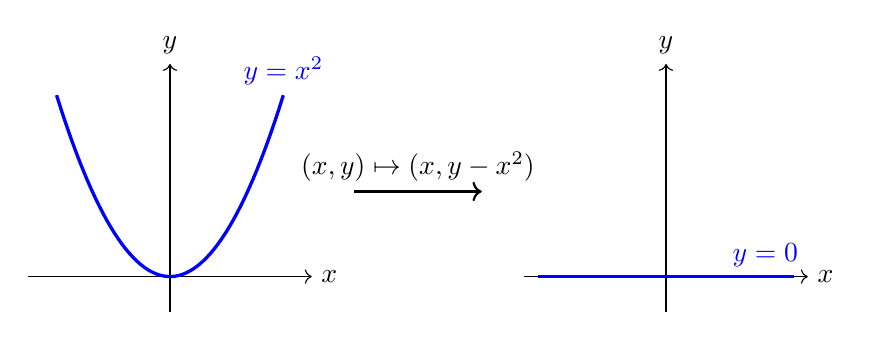
\begin{tikzpicture}[scale=0.9]
  \begin{scope}
    \draw[->] (-2,0)--(2,0) node[right]{$x$};
    \draw[->] (0,-0.5)--(0,3) node[above]{$y$};
    \draw[very thick,blue,domain=-1.6:1.6,samples=60] plot (\x,{\x*\x});
    \node[blue] at (1.6,2.9) {$y=x^2$};
  \end{scope}
  \draw[->,thick] (2.6,1.2)--(4.4,1.2) node[midway,above]{$(x,y)\mapsto(x,y-x^2)$};
  \begin{scope}[xshift=7cm]
    \draw[->] (-2,0)--(2,0) node[right]{$x$};
    \draw[->] (0,-0.5)--(0,3) node[above]{$y$};
    \draw[very thick,blue] (-1.8,0)--(1.8,0);
    \node[blue,above] at (1.4,0) {$y=0$};
  \end{scope}
\end{tikzpicture}
\caption{多項式自己同型による放物線の「まっすぐ化」．}
\label{fig:ch03-parabola-straighten}
\end{figure}

\subsection{アフィン空間上の多項式関数}

多項式 $f\in k[x_1,\dots,x_n]$ は，各点で値を代入することにより関数
\[
  f\colon \A^n\to k,\qquad P=(a_1,\dots,a_n)\mapsto f(P)=f(a_1,\dots,a_n)
\]
を定める．このような関数を \textbf{多項式関数} (polynomial function) あるいは \textbf{正則関数} という．
多項式関数どうしの和・積はまた多項式関数であり，多項式関数全体は $k$ 上の可換環をなす．
この環が多項式環そのものと一致するかどうかは自明ではない．

\begin{myprop}{多項式と多項式関数}{ch03-poly-function}
$k$ が無限体ならば，写像
\[
  k[x_1,\dots,x_n]\longrightarrow \{\A^n\text{ 上の関数}\},\qquad f\mapsto (P\mapsto f(P))
\]
は単射である．すなわち，$\A^n$ の全ての点で値が $0$ になる多項式は零多項式に限る．
\end{myprop}

\begin{proof}
第1章の命題\ref{prop:ch01-poly-function}と同じ主張である（一変数の場合に根の個数が次数以下であることを用い，変数の個数に関する帰納法で示す）．
\end{proof}

有限体ではこの命題は成り立たない．たとえば $k=\F_p$ 上で $f=x^p-x$ は零多項式ではないが，Fermat の小定理により全ての点で $0$ になる．
これが，代数幾何学の素朴な理論を無限体（とくに代数閉体）上で展開する理由の一つである．
有限体上の幾何学をきちんと扱うには，第12章のスキーム論の言葉が必要になる．

\subsection{アフィン空間の幾何学的構造}

$\A^n$ の上に定義される「幾何学的構造」とは何だろうか．微分幾何学では，多様体の構造はその上の滑らかな関数のなす環で決まる．
同様に代数幾何学では，$\A^n$ の構造は
\[
  \text{多項式関数の環}\quad k[\A^n] := k[x_1,\dots,x_n]
\]
によって規定されると考える．距離や角度，あるいは「近さ」といった概念は，あらかじめ与えるものではなく，多項式関数から引き出されるべきものである．
たとえば「点 $P$ の近く」という概念は，「$P$ で $0$ にならない多項式 $f$ について，$f\ne 0$ となる点の集合」という形で定式化される（\ref{sec:ch03-zariski}節の基本開集合）．
また $\A^n$ の部分集合のうちで「意味のある図形」とは，多項式で記述できるもの，すなわち次節以降で扱う零点集合である．

まとめると，本書における基本的な視点は次の対応である：
\begin{center}
\begin{tabular}{c|c}
幾何学 & 代数学 \\ \hline
アフィン空間 $\A^n$ & 多項式環 $k[x_1,\dots,x_n]$ \\
点 $P\in\A^n$ & 値を代入する操作 $f\mapsto f(P)$ \\
図形（代数的集合） & 多項式の集合（イデアル）
\end{tabular}
\end{center}
この対応を精密にすることが本章と第4章の目標である．

\begin{physbox}[配位空間と場の空間]
物理において，$N$ 個のスカラー場 $\phi_1,\dots,\phi_N$ の値の空間（場の空間，target space）は典型的には $\C^N$ であり，
ポテンシャルや超ポテンシャルは $\phi_i$ の多項式で与えられることが多い．
このとき場の空間を「アフィン空間 $\A^N_\C$」として見るのは自然である．
場の再定義 $\phi\mapsto \phi'$ のうち多項式で書けて逆も多項式で書けるものは，ラグランジアンの多項式性を保つ「許される場の再定義」であり，
上で述べた多項式自己同型はちょうどこれに相当する．
\end{physbox}

\exprob{prob:ch03-1} $k=\F_2$ とする．$\A^2_{\F_2}$ の4点すべてで値が $0$ になる零でない多項式 $f\in\F_2[x,y]$ を一つ挙げよ．また，このような $f$ 全体がイデアル $(x^2-x,\ y^2-y)$ と一致することを示せ．

\exprob{prob:ch03-2} 写像 $\varphi\colon\A^2\to\A^2$, $(x,y)\mapsto(x+y^3,\ y)$ が多項式自己同型であることを示し，逆写像を求めよ．また $\varphi$ による曲線 $x=0$ の像を求めよ．

%======================================================================
\section{多項式集合の零点}
%======================================================================

\subsection{多項式集合 $S$ に対する零点集合}

\begin{mydef}{零点集合}{ch03-zero-set}
$S\subset k[x_1,\dots,x_n]$ を多項式の集合とする．
\[
  \Zero(S) := \{P\in\A^n \mid \text{すべての } f\in S \text{ に対し } f(P)=0\}
\]
を $S$ の \textbf{零点集合} (zero locus, vanishing set) という．
$S=\{f_1,\dots,f_r\}$ が有限集合のときは $\Zero(f_1,\dots,f_r)$ と書く．
\end{mydef}

$\Zero(S)$ は「$S$ に属する多項式方程式の連立方程式の解集合」にほかならない．
$S$ は無限集合でも構わないが，後で見るように（命題\ref{prop:ch03-finite-gen}），実は常に有限個の多項式で置き換えられる．

\subsection{単一の多項式が定める集合}

$f$ を定数でない多項式とするとき，$\Zero(f)$ を \textbf{超曲面} (hypersurface) という．
$n=2$ のときは \textbf{平面曲線}，$n=3$ のときは（狭い意味の）\textbf{曲面} である．

\begin{myex}{平面曲線}{ch03-plane-curves}
$\A^2_\R$ の中で次の零点集合を考える（図\ref{fig:ch03-curves}）．
\begin{enumerate}
  \item $\Zero(x^2+y^2-1)$：単位円．
  \item $\Zero(y^2-x^3)$：原点に尖点 (cusp) を持つ曲線．
  \item $\Zero(y^2-x^2(x+1))$：原点で自分自身と交わる曲線（結節点，node）．
  \item $\Zero(xy)$：二本の座標軸の和集合．
\end{enumerate}
$f$ が一つでも，$\Zero(f)$ は滑らかとは限らず（2, 3），いくつかの部分の和集合になることもある（4）．
これらの現象は第7章（特異点）と本章\ref{sec:ch03-irred}節（既約性）でそれぞれ扱う．
\end{myex}

\begin{figure}[H]
\centering
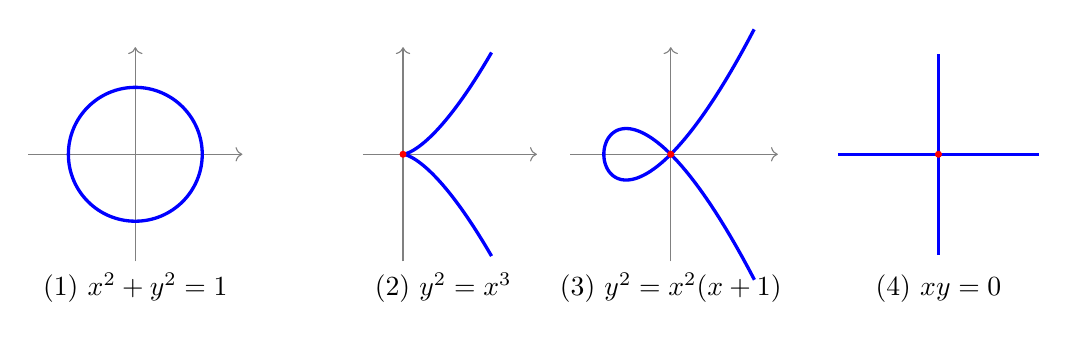
\begin{tikzpicture}[scale=0.85]
  % circle
  \begin{scope}
    \draw[->,gray] (-1.6,0)--(1.6,0); \draw[->,gray] (0,-1.6)--(0,1.6);
    \draw[very thick,blue] (0,0) circle (1);
    \node at (0,-2.0) {(1) $x^2+y^2=1$};
  \end{scope}
  % cusp
  \begin{scope}[xshift=4cm]
    \draw[->,gray] (-0.6,0)--(2,0); \draw[->,gray] (0,-1.6)--(0,1.6);
    \draw[very thick,blue,domain=-1.15:1.15,samples=80] plot ({\x*\x},{\x*\x*\x});
    \fill[red] (0,0) circle (1.5pt);
    \node at (0.6,-2.0) {(2) $y^2=x^3$};
  \end{scope}
  % node
  \begin{scope}[xshift=8cm]
    \draw[->,gray] (-1.5,0)--(1.6,0); \draw[->,gray] (0,-1.6)--(0,1.6);
    \draw[very thick,blue,domain=-1.5:1.5,samples=100] plot ({\x*\x-1},{\x*(\x*\x-1)});
    \fill[red] (0,0) circle (1.5pt);
    \node at (0,-2.0) {(3) $y^2=x^2(x+1)$};
  \end{scope}
  % xy=0
  \begin{scope}[xshift=12cm]
    \draw[very thick,blue] (-1.5,0)--(1.5,0);
    \draw[very thick,blue] (0,-1.5)--(0,1.5);
    \fill[red] (0,0) circle (1.5pt);
    \node at (0,-2.0) {(4) $xy=0$};
  \end{scope}
\end{tikzpicture}
\caption{一つの多項式で定まる平面曲線（実部）．赤い点は特異点．}
\label{fig:ch03-curves}
\end{figure}

\paragraph{超曲面の次元についての直感．}
$\A^n$ の中で方程式を一本課すと自由度が一つ減るので，$\Zero(f)$ は $(n-1)$ 次元の図形になると期待される．
$k$ が代数閉体であれば，定数でない $f$ に対して $\Zero(f)$ は空でなく（一変数ならば代数学の基本定理そのもの），実際 $(n-1)$ 次元になる（次元の厳密な定義と証明は第7章）．
一方 $k=\R$ では $\Zero(x^2+y^2+1)=\emptyset$ や $\Zero(x^2+y^2)=\{(0,0)\}$ のように，次元の直感が破れる．
これが複素数上で考える大きな理由である（第1章参照）．

\subsection{複数の多項式が定める集合}

複数の多項式 $f_1,\dots,f_r$ に対して，定義から直ちに
\[
  \Zero(f_1,\dots,f_r) = \Zero(f_1)\cap\cdots\cap\Zero(f_r)
\]
である．すなわち連立方程式の解集合は各超曲面の共通部分である．

\begin{myex}{空間曲線}{ch03-space-curve}
$\A^3$ において，
\[
  C = \Zero(y-x^2,\ z-x^3)
\]
は二つの曲面 $y=x^2$（放物柱面）と $z=x^3$ の交わりであり，$t\mapsto (t,t^2,t^3)$ と媒介変数表示される曲線である．
これを \textbf{ねじれ3次曲線} (twisted cubic) という．方程式は2本，次元は $3-2=1$ である．
\end{myex}

\begin{myex}{方程式の数と次元が合わない例}{ch03-not-ci}
$\A^3$ において
\[
  X = \Zero(xz,\ yz)
\]
を考える．$xz=yz=0$ は「$z=0$ または $x=y=0$」と同値なので，
$X$ は平面 $\{z=0\}$ と直線 $\{x=y=0\}$（$z$ 軸）の和集合である（図\ref{fig:ch03-plane-line}）．
方程式は2本だが，$X$ には2次元の部分と1次元の部分が混在している．
「方程式の数 $=$ 余次元」という素朴な直感は一般には成り立たない．
\end{myex}

\begin{figure}[H]
\centering
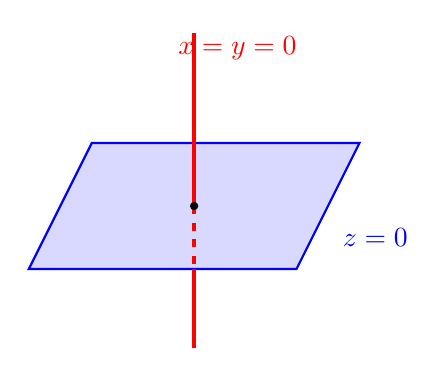
\begin{tikzpicture}[scale=1.0]
  \fill[blue!15] (-2,-0.8)--(1.4,-0.8)--(2.2,0.8)--(-1.2,0.8)--cycle;
  \draw[blue,thick] (-2,-0.8)--(1.4,-0.8)--(2.2,0.8)--(-1.2,0.8)--cycle;
  \draw[very thick,red] (0.1,0)--(0.1,2.2);
  \draw[very thick,red,dashed] (0.1,0)--(0.1,-0.8);
  \draw[very thick,red] (0.1,-0.8)--(0.1,-1.8);
  \node[blue] at (2.4,-0.4) {$z=0$};
  \node[red] at (0.65,2.0) {$x=y=0$};
  \fill (0.1,0) circle (1.5pt);
\end{tikzpicture}
\caption{$\Zero(xz,yz)$：平面と直線の和集合．}
\label{fig:ch03-plane-line}
\end{figure}

\subsection{零点集合の基本性質}

零点集合の基本的な性質をまとめる．$R=k[x_1,\dots,x_n]$ と書く．

\begin{myprop}{零点集合の基本性質}{ch03-zero-props}
$S,T\subset R$，$I,J\subset R$ をイデアルとする．
\begin{enumerate}
  \item（反変性）$S\subset T$ ならば $\Zero(T)\subset\Zero(S)$．
  \item $\Zero(S)=\Zero((S))$．ただし $(S)$ は $S$ で生成されるイデアル．
  \item $\Zero(0)=\A^n$，$\Zero(1)=\emptyset$．
  \item $\Zero(I)\cup\Zero(J)=\Zero(I\cap J)=\Zero(IJ)$．
  \item 任意の族 $\{I_\lambda\}_{\lambda\in\Lambda}$ に対し $\bigcap_\lambda\Zero(I_\lambda)=\Zero\bigl(\sum_\lambda I_\lambda\bigr)$．
\end{enumerate}
\end{myprop}

\begin{proof}
(1) $T$ の全ての元が $P$ で消えれば，$S$ の全ての元も $P$ で消える．

(2) $S\subset(S)$ なので (1) より $\Zero((S))\subset\Zero(S)$．逆に $P\in\Zero(S)$ とする．$(S)$ の元は $g=\sum_i h_if_i$（$h_i\in R$，$f_i\in S$）の形をしており，$g(P)=\sum_i h_i(P)f_i(P)=0$．よって $P\in\Zero((S))$．

(3) 自明．

(4) $IJ\subset I\cap J\subset I$ なので (1) より $\Zero(I)\subset\Zero(I\cap J)\subset\Zero(IJ)$，同様に $\Zero(J)$ についても成り立つから
$\Zero(I)\cup\Zero(J)\subset\Zero(I\cap J)\subset\Zero(IJ)$．
逆に $P\in\Zero(IJ)$ かつ $P\notin\Zero(I)$ とすると，$f(P)\ne0$ となる $f\in I$ がある．任意の $g\in J$ に対し $fg\in IJ$ だから $f(P)g(P)=0$，$k$ は体なので $g(P)=0$．よって $P\in\Zero(J)$．

(5) $P$ が全ての $I_\lambda$ の元で消えることと，それらの有限和 $\sum f_\lambda$ の全てで消えることは同値である．
\end{proof}

(2) により，零点集合を考えるときは多項式の集合 $S$ の代わりにそれが生成するイデアルを考えればよい．
さらに Hilbert の基底定理（第2章）から次が従う．

\begin{myprop}{有限個の方程式で十分}{ch03-finite-gen}
任意の $S\subset k[x_1,\dots,x_n]$ に対し，有限個の $f_1,\dots,f_r\in S$ が存在して $\Zero(S)=\Zero(f_1,\dots,f_r)$ となる．
\end{myprop}

\begin{proof}
$k[x_1,\dots,x_n]$ は Noether 環なので，イデアル $(S)$ は有限生成である．
生成元 $g_1,\dots,g_m$ はそれぞれ $S$ の有限個の元の線形結合で書けるから，それらに現れる $S$ の元を $f_1,\dots,f_r$ とすれば $(S)=(f_1,\dots,f_r)$．
(2) より $\Zero(S)=\Zero((S))=\Zero((f_1,\dots,f_r))=\Zero(f_1,\dots,f_r)$．
\end{proof}

\begin{note}
(4) の等式で $I\cup J$ ではなく $I\cap J$ や $IJ$ が現れることに注意．
「$f=0$ または $g=0$」は「$fg=0$」と同値であるが，これは体（整域）の性質 $ab=0\Rightarrow a=0\text{ または }b=0$ による．
和集合は積に，共通部分は和に対応する：$\Zero(f)\cup\Zero(g)=\Zero(fg)$，$\Zero(f)\cap\Zero(g)=\Zero(f,g)$．
\end{note}

一方，零点集合は多項式の集合を完全には記憶しない．たとえば
\[
  \Zero(x)=\Zero(x^2)=\Zero(x^3)=\cdots=\{0\}\subset\A^1
\]
である．$\Zero$ はイデアルの「冪の違い」を忘れてしまう．この情報の損失を正確に述べたものが第4章の Hilbert の零点定理であり，失われた情報を取り戻す枠組みが第12章のスキーム論である．

\exprob{prob:ch03-3} $\A^2$ において $\Zero(x^2-y,\ x-y)$ と $\Zero(x^2-x,\ xy-y)$ をそれぞれ求めよ．

\exprob{prob:ch03-4} イデアル $I=(x),\ J=(x,y)\subset k[x,y]$ について，$I\cap J$ と $IJ$ を求め，両者が異なるにもかかわらず $\Zero(I\cap J)=\Zero(IJ)$ であることを直接確かめよ．

%======================================================================
\section{代数的集合}
\label{sec:ch03-algset}
%======================================================================

\subsection{代数的集合の定義}

\begin{mydef}{代数的集合}{ch03-algebraic-set}
部分集合 $X\subset\A^n$ が \textbf{(アフィン)代数的集合} (algebraic set) であるとは，
ある多項式の集合 $S\subset k[x_1,\dots,x_n]$ が存在して $X=\Zero(S)$ となることをいう．
命題\ref{prop:ch03-finite-gen}により，このとき $S$ は有限集合に取れる．
\end{mydef}

代数的集合とは「有限個の多項式方程式の共通解として書ける集合」のことである．
文献によってはこれを「アフィン多様体」とよぶこともあるが，本書では既約性などの条件を課したものを第5章で多様体とよぶ．

\begin{myex}{代数的集合の例}{ch03-algset-examples}
\begin{enumerate}
  \item $\A^n=\Zero(0)$，$\emptyset=\Zero(1)$．
  \item 一点 $P=(a_1,\dots,a_n)$：$\{P\}=\Zero(x_1-a_1,\dots,x_n-a_n)$．
  \item 線形部分空間やアフィン部分空間：一次方程式の解集合である．
  \item $\SL_n(k)=\{A\in M_n(k)\mid \det A=1\}\subset\A^{n^2}$ は $\det A-1$ という一つの多項式の零点集合である．
  \item 直交群 $O_n(k)=\{A\mid A^{\mathsf T}A=1\}\subset\A^{n^2}$ は $n(n+1)/2$ 個の二次式の零点集合である．
\end{enumerate}
\end{myex}

一方，代数的集合でない部分集合も多い．

\begin{myex}{代数的集合でない集合}{ch03-not-algset}
\begin{enumerate}
  \item $\Z\subset\A^1_\C$．$\A^1$ の代数的集合は後で見るように有限集合か全体しかない（命題\ref{prop:ch03-A1-closed}）ので，$\Z$ は代数的集合でない．
  \item 正弦曲線 $\Gamma=\{(x,\sin x)\}\subset\A^2_\R$．$\Gamma\subset\Zero(f)$ とする．$-1<c<1$ を満たす任意の $c$ に対し，$\Gamma$ と水平線 $y=c$ の交わりは無限集合なので，一変数多項式 $f(x,c)$ は無限個の根を持ち，恒等的に $0$ である．
        すなわち $f$ は無限本の直線 $y=c$ 上で消える．$f$ を $x$ について整理した各係数（$y$ の多項式）が無限個の根を持つことになるので $f=0$．
        よって $\Gamma$ を含む代数的集合は $\A^2$ 全体のみであり，$\Gamma$ は代数的集合でない．
  \item 上半平面 $\{(x,y)\mid y\ge0\}\subset\A^2_\R$ や単位円板．不等式で定義される集合は（実）代数的集合ではない（半代数的集合とよばれる）．
\end{enumerate}
\end{myex}

\subsection{代数的集合の基本性質}

命題\ref{prop:ch03-zero-props}を代数的集合の言葉で述べ直すと次のようになる．

\begin{mythm}{代数的集合の閉性}{ch03-closed-family}
\begin{enumerate}
  \item $\emptyset$ と $\A^n$ は代数的集合である．
  \item 有限個の代数的集合の和集合は代数的集合である．
  \item 任意個の代数的集合の共通部分は代数的集合である．
\end{enumerate}
\end{mythm}

これは位相空間の閉集合の公理そのものであり，\ref{sec:ch03-zariski}節で Zariski 位相を定義する根拠になる．
無限個の和集合が代数的集合とは限らないことは，$\Z=\bigcup_{m\in\Z}\{m\}\subset\A^1_\C$ の例からわかる．

代数的集合のもう一つの基本性質は \textbf{降鎖条件} である．

\begin{myprop}{代数的集合の降鎖条件}{ch03-dcc}
代数的集合の降鎖 $X_1\supset X_2\supset X_3\supset\cdots$ は必ず有限で止まる．すなわち，ある $N$ があって $X_N=X_{N+1}=\cdots$．
\end{myprop}

\begin{proof}
$X_i$ に対し，$X_i$ 上で消える多項式全体 $\Ideal(X_i)=\{f\mid f|_{X_i}=0\}$ を考えるとこれはイデアルで（第4章で詳しく扱う），
$X_1\supset X_2\supset\cdots$ より $\Ideal(X_1)\subset\Ideal(X_2)\subset\cdots$ はイデアルの昇鎖となる．
$k[x_1,\dots,x_n]$ は Noether 環なので，ある $N$ で $\Ideal(X_N)=\Ideal(X_{N+1})=\cdots$ となる．
一方，代数的集合 $X=\Zero(S)$ について $X=\Zero(\Ideal(X))$ が成り立つ
（$S\subset\Ideal(X)$ より $\Zero(\Ideal(X))\subset\Zero(S)=X$，逆の包含は定義から明らか）．
よって $X_i=\Zero(\Ideal(X_i))$ も $i\ge N$ で一定である．
\end{proof}

\subsection{代数的集合の交}

二つの代数的集合 $X=\Zero(I)$，$Y=\Zero(J)$ の共通部分は
\[
  X\cap Y=\Zero(I+J)=\Zero(I\cup J)
\]
で与えられる．すなわち，方程式を「合併」すればよい．
$I=(f_1,\dots,f_r)$，$J=(g_1,\dots,g_s)$ なら $X\cap Y=\Zero(f_1,\dots,f_r,g_1,\dots,g_s)$ である．

\begin{myex}{放物線と直線の交わり}{ch03-parabola-line}
$\A^2_\C$ において放物線 $X=\Zero(y-x^2)$ と直線 $L_c=\Zero(y-c)$ の交わりは
\[
  X\cap L_c=\Zero(y-x^2,\ y-c)=\Zero(x^2-c,\ y-c)=\{(\pm\sqrt c,\ c)\}
\]
である．$c\ne0$ なら2点，$c=0$ なら1点 $(0,0)$ になる．
$c\to0$ の極限で2点が1点に合流しているので，$c=0$ のときの交点は「重複度2」で数えるのが自然である．
ところが集合としては $\Zero(y-x^2,y)=\Zero(x^2,y)=\Zero(x,y)$ であり，零点集合はこの重複度の情報を失っている．
イデアル $(x^2,y)$ の方は重複度を覚えている（$k[x,y]/(x^2,y)$ が $k$ 上2次元）．これは第9章の交点重複度や第12章のスキームにつながる観点である．
\end{myex}

\begin{figure}[H]
\centering
\begin{tikzpicture}[scale=0.9]
  \draw[->,gray] (-2.2,0)--(2.2,0) node[right]{$x$};
  \draw[->,gray] (0,-0.6)--(0,3.3) node[above]{$y$};
  \draw[very thick,blue,domain=-1.75:1.75,samples=60] plot (\x,{\x*\x});
  \draw[thick,red] (-2.2,1.5)--(2.2,1.5) node[right]{$y=c$};
  \fill[red] ({sqrt(1.5)},1.5) circle (2pt) ({-sqrt(1.5)},1.5) circle (2pt);
  \draw[thick,red,dashed] (-2.2,0.02)--(2.2,0.02);
  \fill[red] (0,0) circle (2pt);
  \node[red,below right] at (0.1,0) {$c=0$：2点が合流};
  \draw[->,red!70] (1.25,1.35)--(0.2,0.2);
\end{tikzpicture}
\caption{放物線と水平線の交わり．$c\to0$ で2つの交点が合流する．}
\label{fig:ch03-parabola-line}
\end{figure}

\subsection{代数的集合の和集合}

和集合については $X\cup Y=\Zero(I\cap J)=\Zero(IJ)$ であった．
生成元で書けば，$I=(f_1,\dots,f_r)$，$J=(g_1,\dots,g_s)$ のとき $IJ=(f_ig_j)_{i,j}$ なので
\[
  X\cup Y=\Zero(f_ig_j\mid 1\le i\le r,\ 1\le j\le s).
\]
「$X$ の方程式が全部成り立つ，または $Y$ の方程式が全部成り立つ」を，積をとることで一つの連立方程式に書き直しているのである．

\begin{myex}{二点の和集合と平面と直線}{ch03-union-examples}
\begin{enumerate}
  \item $\A^1$ の2点 $\{a\}\cup\{b\}=\Zero(x-a)\cup\Zero(x-b)=\Zero((x-a)(x-b))$．
  \item $\A^2$ の2点 $(0,0)$ と $(1,0)$：$\Zero(x,y)\cup\Zero(x-1,y)=\Zero(x(x-1),\ xy,\ y(x-1),\ y^2)$．
        生成元を整理すると $\Zero(x(x-1),\ y)$ に等しい．
  \item 例\ref{ex:ch03-not-ci}の $\Zero(xz,yz)=\Zero(z)\cup\Zero(x,y)$．実際 $(z)\cdot(x,y)=(xz,yz)$ である．
\end{enumerate}
\end{myex}

\subsection{代数的集合の包含関係}

代数的集合の包含関係と多項式の集合の包含関係は \emph{逆向き} に対応する：
方程式を増やせば図形は小さくなる．命題\ref{prop:ch03-zero-props}(1) により $S\subset T\Rightarrow\Zero(T)\subset\Zero(S)$ である．

ただし逆は成り立たない．$\Zero(x^2)\subset\Zero(x)$ であるが $(x)\not\subset(x^2)$．
包含 $\Zero(J)\subset\Zero(I)$ を代数的に判定するには，「$I$ の各元が $\Zero(J)$ 上で消えるか」を調べればよい．
$k$ が代数閉体ならば，これは「$I$ の各元のある冪が $J$ に属するか」，すなわち $I\subset\sqrt{J}$ と同値になる．これが第4章の強零点定理の内容である．

\begin{myex}{包含の判定}{ch03-inclusion}
$X=\Zero(y-x^2)$（放物線），$Y=\Zero(x-1,\ y-1)$（点 $(1,1)$），$Z=\Zero(y^2-x^4)$ とする．
\begin{itemize}
  \item $Y\subset X$：$y-x^2$ に $(1,1)$ を代入すると $0$．
  \item $X\subset Z$：$y^2-x^4=(y-x^2)(y+x^2)\in(y-x^2)$．実際 $Z=X\cup\Zero(y+x^2)$ は二つの放物線の和集合である．
\end{itemize}
したがって $Y\subset X\subset Z$ であり，対応するイデアルは $(y^2-x^4)\subset(y-x^2)\subset(x-1,y-1)$ と逆順に並ぶ．
\end{myex}

\begin{physbox}[真空のモジュライ空間]
超対称ゲージ理論の古典的な真空の集合は，スカラー場 $\phi_i$ の空間の中で F 項条件 $\partial W/\partial\phi_i=0$ と D 項条件で切り出される．
F 項条件は超ポテンシャル $W$ が多項式であれば多項式方程式なので，真空の集合は代数的集合になる．
たとえば $W=\lambda\,\phi\,(\chi^2-v^2)$ なら F 項条件は $\chi^2-v^2=0$，$2\phi\chi=0$ であり，真空は $\Zero(\chi^2-v^2,\ \phi\chi)=\{(\phi,\chi)=(0,\pm v)\}$ の2点である．
$v\to0$ とすると F 項条件は $\chi^2=0,\ \phi\chi=0$ となり，真空の集合は直線 $\{\chi=0\}$（平坦方向）へと大きく変化する．
「方程式の係数を動かすと解集合の形が飛ぶ」という現象は，代数的集合の族として理解される．
\end{physbox}

\exprob{prob:ch03-5} $\A^2$ の3点 $(0,0),(1,0),(0,1)$ からなる集合を，二次式のみを用いた連立方程式の零点集合として表せ．

\exprob{prob:ch03-6} 集合 $\{(x,y)\in\A^2_\C\mid y=e^x\}$ が代数的集合でないことを示せ．（ヒント：直線 $y=1$ との交わりを考えよ．）

%======================================================================
\section{Zariski位相}
\label{sec:ch03-zariski}
%======================================================================

\subsection{位相空間の復習}

集合 $X$ の部分集合の族 $\mathcal{O}$ が次を満たすとき，$\mathcal O$ を $X$ の \textbf{位相} といい，$\mathcal O$ の元を \textbf{開集合} という：
\begin{enumerate}
  \item $\emptyset,\ X\in\mathcal O$，
  \item 任意個の開集合の和集合は開集合，
  \item 有限個の開集合の共通部分は開集合．
\end{enumerate}
開集合の補集合を \textbf{閉集合} という．De Morgan の法則により，閉集合の族 $\mathcal F$ は
(i) $\emptyset,X\in\mathcal F$，(ii) 有限個の和集合で閉じる，(iii) 任意個の共通部分で閉じる，を満たし，
逆にこれらを満たす族 $\mathcal F$ を閉集合系として位相が一意に定まる．

部分集合 $A\subset X$ の \textbf{閉包} $\overline{A}$ は $A$ を含む最小の閉集合（$A$ を含む閉集合全ての共通部分）である．
$\overline A=X$ のとき $A$ は \textbf{稠密} であるという．
$X$ が \textbf{Hausdorff} であるとは，任意の異なる2点 $P\ne Q$ に対し，互いに交わらない開集合 $U\ni P$，$V\ni Q$ が存在することをいう．
$X$ が \textbf{準コンパクト} であるとは，任意の開被覆が有限部分被覆を持つことをいう（Hausdorff を仮定しないコンパクト性）．
部分集合 $Y\subset X$ には $\{U\cap Y\mid U\in\mathcal O\}$ を開集合系とする \textbf{相対位相} が入る．

物理学で普段使う $\R^n$ や $\C^n$ の位相（Euclid 位相）は距離から定まる位相であり，Hausdorff である．
以下ではこれを \textbf{通常の位相}（あるいは古典位相，複素位相）とよび，Zariski 位相と区別する．

\subsection{Zariski閉集合}

\begin{mydef}{Zariski閉集合}{ch03-zariski-closed}
$\A^n$ の代数的集合，すなわち $\Zero(S)$ の形の部分集合を \textbf{Zariski閉集合} という．
\end{mydef}

定理\ref{thm:ch03-closed-family}により，Zariski閉集合の全体は閉集合系の公理 (i)--(iii) を満たす．
より一般に，代数的集合 $X\subset\A^n$ に対し，$X$ に含まれる代数的集合を $X$ の Zariski 閉集合という．

\subsection{Zariski位相の定義}

\begin{mydef}{Zariski位相}{ch03-zariski}
Zariski閉集合全体を閉集合系とする $\A^n$ の位相を \textbf{Zariski位相} (Zariski topology) という．
代数的集合 $X\subset\A^n$ には，その相対位相を入れ，これを $X$ の Zariski 位相とよぶ．
$X$ の閉集合はちょうど $X$ に含まれる代数的集合であり，$X\cap\Zero(S)=\Zero(\Ideal(X)\cup S)$ の形をしている．
\end{mydef}

Zariski位相は「多項式関数が連続になる最も粗い位相」（ただし $k$ に有限集合と全体のみを閉集合とする位相を入れる）と言い換えることもできる．
実際，多項式 $f$ に対し $f^{-1}(c)=\Zero(f-c)$ は閉集合だからである．

\begin{myprop}{$\A^1$ のZariski位相}{ch03-A1-closed}
$k$ を無限体とする．$\A^1$ の Zariski 閉集合は，$\A^1$ 自身と有限部分集合（空集合を含む）に限る．
したがって $\A^1$ の空でない開集合は有限個の点を除いた集合（補有限集合）である．
\end{myprop}

\begin{proof}
$X=\Zero(S)$，$S\subset k[x]$ とする．$S\subset\{0\}$ ならば $X=\A^1$．
$S$ が零でない $f$ を含めば $X\subset\Zero(f)$ であり，$\Zero(f)$ は $f$ の根の集合で高々 $\deg f$ 個の元からなる．よって $X$ は有限集合．
逆に有限集合 $\{a_1,\dots,a_m\}=\Zero\bigl(\prod_i(x-a_i)\bigr)$ は閉集合である．
\end{proof}

つまり $\A^1$ の Zariski 位相は \textbf{補有限位相} (cofinite topology) にほかならない．
$\A^1_\C=\C$ で言えば，通常の位相で閉である円周 $|z|=1$ や実軸 $\R\subset\C$ も，Zariski 位相では閉集合ではない．
実軸を含む最小の Zariski 閉集合は $\C$ 全体，すなわち $\R$ は $\A^1_\C$ で \emph{Zariski 稠密} である．

\subsection{Zariski開集合}

Zariski 閉集合の補集合を \textbf{Zariski開集合} という．特に重要なのは一つの多項式で定まる開集合である．

\begin{mydef}{基本開集合}{ch03-basic-open}
$f\in k[x_1,\dots,x_n]$ に対し
\[
  D(f):=\A^n\setminus\Zero(f)=\{P\in\A^n\mid f(P)\ne0\}
\]
を \textbf{基本開集合} (basic open set, principal open set) という．
\end{mydef}

\begin{myprop}{基本開集合は開基をなす}{ch03-basis}
\begin{enumerate}
  \item $D(f)\cap D(g)=D(fg)$．
  \item $\A^n$ の任意の Zariski 開集合は有限個の基本開集合の和集合である．
\end{enumerate}
特に基本開集合全体は Zariski 位相の開基をなす．
\end{myprop}

\begin{proof}
(1) $f(P)g(P)\ne0\iff f(P)\ne0$ かつ $g(P)\ne0$．
(2) 開集合 $U$ に対し $\A^n\setminus U=\Zero(f_1,\dots,f_r)$（命題\ref{prop:ch03-finite-gen}）と書けるので，
$U=\A^n\setminus\bigcap_i\Zero(f_i)=\bigcup_i D(f_i)$．
\end{proof}

\begin{myex}{開集合の例}{ch03-open-examples}
\begin{enumerate}
  \item $D(x)=\A^1\setminus\{0\}$．これは $k^\times$ であり，物理では「$\C^\times$ 上の理論」として頻出する．
  \item $\GL_n(k)=D(\det)\subset\A^{n^2}$．可逆行列全体は Zariski 開集合である．
  \item $\A^2$ から原点を除いた $U=\A^2\setminus\{(0,0)\}=D(x)\cup D(y)$．$U$ は基本開集合ではない（$\{(0,0)\}=\Zero(f)$ となる多項式 $f$ は存在しない．$k$ が代数閉なら $\Zero(f)$ は空か1次元だからである）．
\end{enumerate}
\end{myex}

\begin{physbox}[一般の点と特別な点]
物理でパラメータ空間を考えるとき，「一般的な (generic) パラメータでは対称性が破れていて，特別な値でのみ対称性が回復する」という状況がよく現れる．
たとえば行列 $M$ の固有値が縮退する条件は判別式 $\Delta(M)=0$ という多項式方程式で書ける．
このとき縮退が起こる点の集合 $\Zero(\Delta)$ は Zariski 閉集合であり，縮退しない点の集合 $D(\Delta)$ は Zariski 開かつ稠密である．
物理学者の言う「generic」とは，多くの場合「空でない Zariski 開集合に属する」ことを意味すると考えてよい．
\end{physbox}

\subsection{Zariski位相と通常の位相の比較}

$k=\C$ とする．多項式は連続関数なので，$\Zero(f)=f^{-1}(0)$ は通常の位相で閉集合であり，その任意個の共通部分も閉である．したがって

\begin{myprop}{Zariski位相は通常の位相より粗い}{ch03-coarser}
$\A^n_\C$ の Zariski 閉（開）集合は通常の位相でも閉（開）である．逆は成り立たない．
\end{myprop}

逆が成り立たない例は，閉円板 $\{|z|\le1\}\subset\C$ や実軸 $\R\subset\C$ である．
Zariski 開集合は「非常に大きい」：空でない Zariski 開集合は通常の位相で稠密である（例えば $D(f)$ は超曲面 $\Zero(f)$ を除いた集合であり，$\Zero(f)$ は内点を持たない）．

最も顕著な違いは次の性質である．

\begin{myprop}{非Hausdorff性}{ch03-non-hausdorff}
$k$ を無限体，$n\ge1$ とする．$\A^n$ の任意の二つの空でない Zariski 開集合は交わる．
特に $\A^n$ は Hausdorff でない．
\end{myprop}

\begin{proof}
空でない開集合 $U,V$ は基本開集合 $D(f)\subset U$，$D(g)\subset V$（$f,g\ne0$）を含む．
$D(f)\cap D(g)=D(fg)$ であり，$fg\ne0$ なので命題\ref{prop:ch03-poly-function}により $fg(P)\ne0$ となる点 $P$ が存在する．よって $U\cap V\ne\emptyset$．
\end{proof}

図\ref{fig:ch03-nonhausdorff}は $\A^1$ における状況を示している．
二点 $P,Q$ を分離しようとして $P$ の開近傍 $U$ を取っても，$U$ は有限個の点を除いた全体なので，$Q$ のどんな開近傍とも（実際無限個の点で）交わってしまう．

\begin{figure}[H]
\centering
\begin{tikzpicture}[scale=1.0]
  \begin{scope}
    \node at (2.5,1.2) {通常の位相（Hausdorff）};
    \draw[thick] (0,0)--(5,0);
    \fill (1.5,0) circle (2pt) node[below]{$P$};
    \fill (3.5,0) circle (2pt) node[below]{$Q$};
    \draw[blue,thick] (1.5,0) ellipse (0.6 and 0.3);
    \draw[red,thick] (3.5,0) ellipse (0.6 and 0.3);
    \node[blue] at (1.5,0.55) {$U$}; \node[red] at (3.5,0.55) {$V$};
  \end{scope}
  \begin{scope}[xshift=7cm]
    \node at (2.5,1.2) {Zariski位相};
    \draw[blue,line width=3pt,opacity=0.35] (0,0.08)--(5,0.08);
    \draw[red,line width=3pt,opacity=0.35] (0,-0.08)--(5,-0.08);
    \foreach \t in {0.6,2.6,4.3} {\fill[white] (\t,0.08) circle (2.5pt); \draw[blue] (\t,0.08) circle (2.5pt);}
    \foreach \t in {1.1,3.1,4.0} {\fill[white] (\t,-0.08) circle (2.5pt); \draw[red] (\t,-0.08) circle (2.5pt);}
    \fill (1.5,0) circle (2pt) node[below=3pt]{$P$};
    \fill (3.5,0) circle (2pt) node[below=3pt]{$Q$};
    \node[blue] at (0.3,0.45) {$U$}; \node[red] at (0.3,-0.45) {$V$};
  \end{scope}
\end{tikzpicture}
\caption{$\A^1$ における点の分離．Zariski 開集合は有限個の点（白丸）を除いた全体なので，$P$ と $Q$ の近傍は必ず交わる．}
\label{fig:ch03-nonhausdorff}
\end{figure}

\paragraph{$\A^2$ の位相は $\A^1\times\A^1$ の積位相ではない．}
集合としては $\A^2=\A^1\times\A^1$ であるが，Zariski 位相は積位相より真に細かい．
積位相における閉集合は，$\A^1$ の閉集合（有限集合または全体）の積 $F_1\times F_2$ の有限和とその任意の共通部分である．
具体的には，積位相の閉集合は「有限個の点，有限個の水平線 $\{y=b\}$，有限個の垂直線 $\{x=a\}$」の和集合（および全体）に限られる．
ところが対角線 $\Delta=\Zero(x-y)$ や放物線 $\Zero(y-x^2)$ は Zariski 閉集合であるが，積位相では閉でない（図\ref{fig:ch03-product}）．
これは，代数幾何学では「直積」を位相の直積として定義してはならないことを示している．
正しい直積は座標環のテンソル積 $k[x]\otimes_k k[y]=k[x,y]$ に基づいて定義される（第5章，第12章）．

\begin{figure}[H]
\centering
\begin{tikzpicture}[scale=0.9]
  \begin{scope}
    \draw[->,gray] (-0.2,0)--(3.4,0); \draw[->,gray] (0,-0.2)--(0,3.4);
    \draw[thick,blue] (0.8,-0.2)--(0.8,3.3);
    \draw[thick,blue] (2.3,-0.2)--(2.3,3.3);
    \draw[thick,blue] (-0.2,1.9)--(3.3,1.9);
    \fill[blue] (1.6,0.7) circle (2pt);
    \node at (1.6,-0.8) {積位相の閉集合};
  \end{scope}
  \begin{scope}[xshift=5.5cm]
    \draw[->,gray] (-0.2,0)--(3.4,0); \draw[->,gray] (0,-0.2)--(0,3.4);
    \draw[thick,red] (-0.2,-0.2)--(3.3,3.3) node[right]{$x=y$};
    \draw[thick,red,domain=0:1.8,samples=40] plot (\x,{\x*\x});
    \node[red] at (2.4,3.2) {$y=x^2$};
    \node at (1.6,-0.8) {Zariski 閉だが積位相で閉でない};
  \end{scope}
\end{tikzpicture}
\caption{$\A^1\times\A^1$ の積位相と $\A^2$ の Zariski 位相．}
\label{fig:ch03-product}
\end{figure}

\subsection{Zariski位相の特徴}

Zariski 位相の主な特徴をまとめておく．

\begin{myprop}{Zariski位相の性質}{ch03-zariski-props}
$X\subset\A^n$ を代数的集合とし，Zariski 位相を入れる．
\begin{enumerate}
  \item（$T_1$ 性）一点集合は閉集合である．
  \item（Noether性）$X$ の閉集合の降鎖は有限で止まる．同値なことに開集合の昇鎖は有限で止まる．
  \item（準コンパクト性）$X$ の任意の部分集合は準コンパクトである．
  \item 多項式写像 $\varphi\colon\A^n\to\A^m$，$P\mapsto(\varphi_1(P),\dots,\varphi_m(P))$ は Zariski 位相について連続である．
\end{enumerate}
\end{myprop}

\begin{proof}
(1) 例\ref{ex:ch03-algset-examples}(2)．(2) 命題\ref{prop:ch03-dcc}．

(3) $Y\subset X$ と $Y$ の開被覆 $\{U_\lambda\}$ を取る．有限個の $U_\lambda$ の和集合全体の族を考えると，(2) より（開集合の昇鎖条件から）この族には包含に関する極大元 $U=U_{\lambda_1}\cup\cdots\cup U_{\lambda_r}$ が存在する（極大元がなければ真の昇鎖が無限に作れる）．
もし $U\ne Y$ なら $U\cup U_\mu\supsetneq U$ となる $U_\mu$ があり極大性に反する．よって $U=Y$．

(4) 閉集合 $\Zero(g_1,\dots,g_s)\subset\A^m$ の逆像は $\Zero(g_1\circ\varphi,\dots,g_s\circ\varphi)$ であり，$g_j\circ\varphi$ は多項式なので閉集合である．
\end{proof}

(3) の準コンパクト性は，$\C^n$ が通常の位相ではコンパクトでないことと対照的である．Zariski 位相では「開集合が大きすぎる」ためにこのような現象が起こる．

\begin{note}
Zariski 位相は粗すぎるため，通常の位相で使える議論（たとえば陰関数定理や，点の小さな近傍での議論）はそのままでは使えない．
その代わりに代数幾何学では，局所環（第6章）や接空間（第7章）といった代数的な道具で「局所的」な性質を捉える．
一方，「空でない開集合は稠密」という性質は，「ある一点で成り立つ開条件は一般の点で成り立つ」という強力な原理を与える．
\end{note}

\exprob{prob:ch03-7} $\A^1$ の部分集合 $A$ の Zariski 閉包を求めよ：(a) $A=\{1,2,3\}$，(b) $A=\Z$（$k=\C$），(c) $A=\{z\in\C\mid|z|=1\}$．

\exprob{prob:ch03-8} $\A^2_\C$ において，集合 $\{(t,t^2)\mid t\in\R\}$ の Zariski 閉包を求めよ．

%======================================================================
\section{既約性}
\label{sec:ch03-irred}
%======================================================================

\subsection{既約な位相空間}

$\Zero(xy)$ は二本の直線の和集合であり，「二つの部分に分かれている」．
一方，通常の位相では $\Zero(xy)$ は連結である．
連結性とは別の意味での「分かれ方」を捉えるのが既約性である．

\begin{mydef}{既約な位相空間}{ch03-irreducible-space}
位相空間 $X$ が \textbf{既約} (irreducible) であるとは，$X\ne\emptyset$ であり，
$X=X_1\cup X_2$（$X_1,X_2$ は閉集合）と書けるならば $X=X_1$ または $X=X_2$ となることをいう．
既約でない空でない空間を \textbf{可約} (reducible) という．
部分集合 $Y\subset X$ が既約であるとは，相対位相で既約であることをいう．
\end{mydef}

\begin{mylem}{既約性の言い換え}{ch03-irred-equiv}
空でない位相空間 $X$ について次は同値である．
\begin{enumerate}
  \item $X$ は既約．
  \item 任意の二つの空でない開集合 $U,V\subset X$ は交わる．
  \item 任意の空でない開集合は $X$ で稠密である．
\end{enumerate}
\end{mylem}

\begin{proof}
(1)$\Rightarrow$(2)：$U\cap V=\emptyset$ ならば $X=(X\setminus U)\cup(X\setminus V)$ で，既約性から $X\setminus U=X$ または $X\setminus V=X$，すなわち $U$ か $V$ が空．
(2)$\Rightarrow$(3)：$U$ が稠密でなければ $V=X\setminus\overline U$ は空でない開集合で $U\cap V=\emptyset$．
(3)$\Rightarrow$(1)：$X=X_1\cup X_2$（閉）で $X_1\ne X$ とすると，$U=X\setminus X_1$ は空でない開集合で $U\subset X_2$．$U$ は稠密なので $X=\overline U\subset X_2$．
\end{proof}

Hausdorff 空間で既約なのは一点だけである（二点あれば分離する開集合が取れるから）．したがって既約性は Zariski 位相のような非 Hausdorff な位相に特有の概念である．
命題\ref{prop:ch03-non-hausdorff}は，まさに「$\A^n$ は既約である」と言っている．

\begin{mylem}{既約性の基本性質}{ch03-irred-basic}
$X$ を位相空間とする．
\begin{enumerate}
  \item $Y\subset X$ が既約ならば，その閉包 $\overline Y$ も既約．
  \item 既約空間の空でない開集合は既約かつ稠密．
  \item $X$ が既約で $f\colon X\to Z$ が連続ならば，$f(X)$ は既約．
\end{enumerate}
\end{mylem}

\begin{proof}
(1) $\overline Y=F_1\cup F_2$（閉）なら $Y=(Y\cap F_1)\cup(Y\cap F_2)$ で，$Y$ の既約性から例えば $Y\subset F_1$．$F_1$ は閉なので $\overline Y\subset F_1$．
(2) 補題\ref{lem:ch03-irred-equiv}(2) を開集合 $U$ に適用すればよい（$U$ の開集合は $X$ の開集合でもある）．
(3) $f(X)=F_1\cup F_2$（$f(X)$ の閉集合）なら $X=f^{-1}(F_1)\cup f^{-1}(F_2)$ で，例えば $X=f^{-1}(F_1)$，よって $f(X)=F_1$．
\end{proof}

\subsection{既約代数的集合}

代数的集合 $X\subset\A^n$ が既約であるとは，Zariski 位相について既約であること，すなわち
\[
  X=X_1\cup X_2\ (X_i\text{ は代数的集合})\ \Longrightarrow\ X=X_1\ \text{または}\ X=X_2
\]
が成り立つことである．直感的には「これ以上真に小さい代数的集合の和に分けられない図形」である．

\begin{myex}{既約・可約の例}{ch03-irred-ex}
\begin{enumerate}
  \item 一点は既約．$\A^n$ は既約（命題\ref{prop:ch03-non-hausdorff}と補題\ref{lem:ch03-irred-equiv}）．
  \item $\Zero(xy)=\Zero(x)\cup\Zero(y)$ は可約．
  \item 有限集合は点が2個以上あれば可約．
  \item 放物線 $C=\Zero(y-x^2)$ は既約．実際，$\varphi\colon\A^1\to\A^2$，$t\mapsto(t,t^2)$ は多項式写像で連続（命題\ref{prop:ch03-zariski-props}(4)），像は $C$．$\A^1$ が既約なので補題\ref{lem:ch03-irred-basic}(3) から $C$ も既約．
\end{enumerate}
\end{myex}

例 (4) の議論は一般化できる：\textbf{多項式でパラメータ付けされる集合は既約である}．
ねじれ3次曲線 $t\mapsto(t,t^2,t^3)$ や尖点曲線 $t\mapsto(t^2,t^3)$ の像も既約である．
（像が閉集合であることは別途確認が要るが，これらの例では像はちょうど $\Zero(y-x^2,z-x^3)$，$\Zero(y^2-x^3)$ に一致する．）

\subsection{既約成分}

\begin{mydef}{既約成分}{ch03-irred-component}
位相空間 $X$ の既約部分集合のうち，包含関係について極大なものを $X$ の \textbf{既約成分} (irreducible component) という．
\end{mydef}

補題\ref{lem:ch03-irred-basic}(1) より，既約成分は必ず閉集合である（$\overline Y$ も既約で $Y\subset\overline Y$ なので極大性より $Y=\overline Y$）．
また，任意の既約部分集合はある既約成分に含まれる（Zorn の補題による；既約集合の鎖の和は既約である）．

\begin{myex}{既約成分の例}{ch03-component-ex}
\begin{enumerate}
  \item $\Zero(xy)\subset\A^2$ の既約成分は二直線 $\Zero(x)$ と $\Zero(y)$．
  \item $\Zero(xz,yz)\subset\A^3$ の既約成分は平面 $\Zero(z)$ と直線 $\Zero(x,y)$（例\ref{ex:ch03-not-ci}）．次元の異なる成分が共存しうる．
  \item 有限集合の既約成分は各点．
\end{enumerate}
\end{myex}

既約成分どうしは交わってよい（例 (1) の原点）．この点が連結成分との大きな違いである．
連結成分は互いに交わらないが，既約成分は「部品どうしが接着されている」状況を表現できる．

\subsection{既約分解}

\begin{mydef}{Noether位相空間}{ch03-noetherian-space}
位相空間 $X$ の閉集合の任意の降鎖 $Z_1\supset Z_2\supset\cdots$ が有限で止まるとき，$X$ を \textbf{Noether位相空間} という．
\end{mydef}

命題\ref{prop:ch03-zariski-props}(2) により，代数的集合は Zariski 位相で Noether 位相空間である．
Noether 性は次の \textbf{Noether 帰納法} を可能にする：
\begin{quote}
$X$ の閉集合の空でない族 $\Sigma$ は包含関係について極小元を持つ．
\end{quote}
（極小元がなければ $Z_1\supsetneq Z_2\supsetneq\cdots$ と無限降鎖が作れてしまう．）

\begin{mythm}{既約分解の存在と一意性}{ch03-irred-decomp}
$X$ を空でない Noether 位相空間とする．このとき $X$ は有限個の既約閉集合の和
\[
  X=X_1\cup X_2\cup\cdots\cup X_r,\qquad X_i\not\subset X_j\ (i\ne j)
\]
として表され，このような表示（\textbf{無駄のない既約分解}）は順序を除いて一意である．
さらに $X_1,\dots,X_r$ はちょうど $X$ の既約成分の全体である．
特に，任意の代数的集合は有限個の既約代数的集合の無駄のない和として一意的に表される．
\end{mythm}

\begin{proof}
\textbf{存在．}有限個の既約閉集合の和として書けない空でない閉集合 $Z\subset X$ の族を $\Sigma$ とし，$\Sigma\ne\emptyset$ と仮定する．
Noether 性から $\Sigma$ は極小元 $Z$ を持つ．$Z$ は既約ではない（既約ならそれ自身が1個の和）から，$Z=Z'\cup Z''$（$Z',Z''\subsetneq Z$ は閉）と書ける．
$Z',Z''$ は空でない（空なら他方が $Z$ に等しい）．極小性から $Z',Z''\notin\Sigma$ なので，それぞれ有限個の既約閉集合の和であり，したがって $Z$ もそうである．矛盾．
よって $X$ は $X=X_1\cup\cdots\cup X_r$（$X_i$ 既約閉）と書ける．$X_i\subset X_j$（$i\ne j$）となるものがあれば $X_i$ を取り除けばよいので，無駄のない表示が得られる．

\textbf{一意性．}$X=X_1\cup\cdots\cup X_r=Y_1\cup\cdots\cup Y_s$ を二つの無駄のない既約分解とする．
$X_1=\bigcup_j(X_1\cap Y_j)$ であり，$X_1\cap Y_j$ は $X_1$ の閉集合なので，$X_1$ の既約性から $X_1\subset Y_j$ となる $j$ がある（有限和への帰納的適用）．
同様に $Y_j\subset X_i$ となる $i$ があり，$X_1\subset Y_j\subset X_i$．無駄のなさから $i=1$，よって $X_1=Y_j$．
これを全ての $X_i$ に行えば $\{X_i\}\subset\{Y_j\}$，対称性から逆も成り立つ．

\textbf{既約成分との一致．}$Y\subset X$ が既約ならば，上と同じ議論で $Y\subset X_i$ となる $i$ がある．
したがって極大な既約部分集合は $X_i$ のいずれかに一致する．逆に各 $X_i$ が極大であることは，$X_i\subset Y$（$Y$ 既約）なら $Y\subset X_j$ となる $j$ があり $X_i\subset X_j$，よって $i=j$ かつ $Y=X_i$ となることからわかる．
\end{proof}

\begin{figure}[H]
\centering
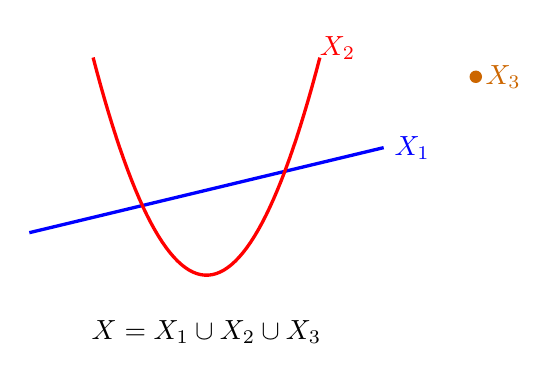
\begin{tikzpicture}[scale=0.9]
  \draw[very thick,blue] (-2.5,-0.6) -- (2.5,0.6) node[right]{$X_1$};
  \draw[very thick,red,domain=-1.6:1.6,samples=60] plot (\x,{1.2*\x*\x-1.2}) ;
  \node[red] at (1.85,2.0) {$X_2$};
  \fill[orange!80!black] (3.8,1.6) circle (2.5pt) node[right]{$X_3$};
  \node at (0,-2.0) {$X=X_1\cup X_2\cup X_3$};
\end{tikzpicture}
\caption{既約分解の模式図．直線 $X_1$，曲線 $X_2$，孤立点 $X_3$．既約成分は交わってもよく，次元が異なってもよい．}
\label{fig:ch03-decomp}
\end{figure}

図\ref{fig:ch03-decomp}のような集合は例えば
$X=\Zero(y)\cup\Zero(y-x^2+1)\cup\{(3,1)\}$ として実現される．

\subsection{既約性と整域}

既約性を多項式の言葉で特徴づけよう．代数的集合 $X\subset\A^n$ に対し
\[
  \Ideal(X):=\{f\in k[x_1,\dots,x_n]\mid \text{全ての } P\in X \text{ で } f(P)=0\}
\]
を $X$ の \textbf{消滅イデアル} とよぶ．
$\Ideal(X)$ がイデアルであることは容易に確かめられる．消滅イデアルの詳しい性質は第4章で扱う．
ここで必要なのは次の二つだけである（命題\ref{prop:ch03-dcc}の証明で示した）：
\[
  X\subset Y\Rightarrow \Ideal(Y)\subset\Ideal(X),\qquad X=\Zero(\Ideal(X))\quad(X\text{ は代数的集合}).
\]
後者から，代数的集合については $X\subsetneq Y\Rightarrow\Ideal(Y)\subsetneq\Ideal(X)$ が従う．

\begin{mythm}{既約性と素イデアル}{ch03-irred-prime}
代数的集合 $X\subset\A^n$ について，次は同値である．
\begin{enumerate}
  \item $X$ は既約である．
  \item $\Ideal(X)$ は素イデアルである．
  \item 剰余環 $k[X]:=k[x_1,\dots,x_n]/\Ideal(X)$ は整域である．
\end{enumerate}
\end{mythm}

\begin{proof}
(2)$\Leftrightarrow$(3) は素イデアルの定義と剰余環の性質（第2章）から直ちに従う．

(1)$\Rightarrow$(2)：$X\ne\emptyset$ なので $1\notin\Ideal(X)$．$fg\in\Ideal(X)$ とすると
$X\subset\Zero(fg)=\Zero(f)\cup\Zero(g)$ なので
\[
  X=(X\cap\Zero(f))\cup(X\cap\Zero(g))
\]
は閉集合二つの和．既約性から，例えば $X=X\cap\Zero(f)$，すなわち $f$ は $X$ 上で消え $f\in\Ideal(X)$．

(2)$\Rightarrow$(1)：$\Ideal(X)$ は真のイデアルなので $X\ne\emptyset$（$\Ideal(\emptyset)=k[x_1,\dots,x_n]$）．
$X=X_1\cup X_2$（$X_i$ は代数的集合）で $X_1\ne X$，$X_2\ne X$ と仮定する．
上の注意から $\Ideal(X)\subsetneq\Ideal(X_i)$ なので，$f_i\in\Ideal(X_i)\setminus\Ideal(X)$ が取れる．
すると $f_1f_2$ は $X_1$ 上でも $X_2$ 上でも消えるので $f_1f_2\in\Ideal(X)$．しかし $f_1,f_2\notin\Ideal(X)$ であり，$\Ideal(X)$ が素であることに反する．
\end{proof}

剰余環 $k[X]$ は $X$ の \textbf{座標環} とよばれ，$X$ 上の多項式関数の環とみなせる（第4章で導入し，第5章で詳しく扱う）．
定理\ref{thm:ch03-irred-prime}は
\begin{center}
「図形が二つに分かれる」$\iff$「零でない二つの関数の積が零になる」
\end{center}
という直感的な対応を述べている．実際 $X=\Zero(xy)$ 上では関数 $x$ と $y$ はどちらも恒等的に $0$ ではないが，積 $xy$ は $X$ 上で恒等的に $0$ である：$x$ は直線 $\Zero(y)$ 上でのみ非零，$y$ は直線 $\Zero(x)$ 上でのみ非零で，台が別々の成分に分かれている．

\begin{physbox}[Higgs branch と Coulomb branch]
超対称ゲージ理論の真空のモジュライ空間は，しばしば複数の既約成分からなる．
典型例は，ゲージ不変量で書いたときに $\Zero(xy)\subset\A^2$ のような形になる場合である：
一方の成分（$y=0$，$x$ が自由）ではベクトル多重項のスカラー $x$ が値を持ち，ゲージ群は可換な部分群（Cartan部分群）までしか破れない（Coulomb branch に相当）．
もう一方の成分（$x=0$）ではハイパー多重項のスカラーが値を持ちゲージ群が Higgs 機構で破れる（Higgs branch に相当）．
二つの既約成分は原点で交わり，そこでは余分な粒子が質量ゼロになる．
既約分解は，「物理的に異なる相（branch）が何個あり，どこで接続しているか」を数学的に記述する言語である．
\end{physbox}

\exprob{prob:ch03-9} $X=\Zero(x^2-yz,\ xz-x)\subset\A^3$ の既約分解を求めよ．

\exprob{prob:ch03-10} 既約な位相空間は連結であることを示せ．また，連結だが既約でない代数的集合の例を挙げよ．

%======================================================================
\section{代数的集合の具体例}
%======================================================================

本節では，これまでの概念を具体例で確認する．以下 $k$ は代数閉体で，$\mathrm{char}\,k\ne2$ とする（二次形式の標準形を使うため）．

\subsection{直線と平面}

$\A^n$ の \textbf{アフィン部分空間}（直線・平面・超平面など）は一次方程式系
\[
  \sum_{j=1}^n a_{ij}x_j=b_i\qquad(i=1,\dots,r)
\]
の解集合である．解が存在すれば，それは $d=n-\rank(a_{ij})$ 次元のパラメータ表示
\[
  \bm x=\bm p+t_1\bm v_1+\cdots+t_d\bm v_d
\]
を持つ．これは多項式（一次式）写像 $\A^d\to\A^n$ の像であり，$\A^d$ が既約なので，\textbf{アフィン部分空間は既約} である．
また消滅イデアルは一次式で生成される素イデアルであり，座標を取り替えれば $(x_{d+1},\dots,x_n)$ の形になる．
このとき座標環は $k[x_1,\dots,x_n]/(x_{d+1},\dots,x_n)\cong k[x_1,\dots,x_d]$，すなわち $d$ 次元アフィン空間の座標環である．

\begin{myex}{二平面の交わり}{ch03-two-planes}
$\A^3$ の二平面 $H_1=\Zero(x+y+z-1)$，$H_2=\Zero(x-y)$ の交わりは
\[
  H_1\cap H_2=\Zero(x+y+z-1,\ x-y)=\{(t,\ t,\ 1-2t)\mid t\in k\}
\]
という直線である．平行な二平面 $\Zero(z)$ と $\Zero(z-1)$ の交わりは $\Zero(z,z-1)=\Zero(1)=\emptyset$ である．
このように，アフィン空間では「平行なものは交わらない」という例外が生じる．射影空間（第8章）に移るとこの例外が消える．
\end{myex}

\subsection{二次曲線}

$\A^2$ の二次曲線は $f(x,y)=ax^2+bxy+cy^2+dx+ey+g=0$（$(a,b,c)\ne0$）で定義される．
$k$ が代数閉体ならば，アフィン変換により $f$ は次のいずれかの標準形に変換できる：
\begin{center}
\begin{tabular}{lll}
標準形 & 名前 & 既約性 \\ \hline
$xy-1$ （または $x^2+y^2-1$） & 非退化中心二次曲線 & 既約 \\
$y-x^2$ & 放物線 & 既約 \\
$xy$ & 交わる二直線 & 可約 \\
$x^2-1$ & 平行な二直線 & 可約 \\
$x^2$ & 二重直線 & 既約（集合として直線）
\end{tabular}
\end{center}
代数閉体上では楕円と双曲線の区別は消える：$k=\C$ で $u=x+iy$，$v=x-iy$ と置けば $x^2+y^2-1=uv-1$ である．
実際，実の円 $x^2+y^2=1$ の複素化は，$\C^2$ の中では双曲線 $uv=1$ と同型な曲線で，これは $\C^\times$ と同型である（$u\in\C^\times$ を与えれば $v=1/u$）．

\begin{myex}{双曲線の既約性}{ch03-hyperbola}
$X=\Zero(xy-1)$ は既約である．実際，$\varphi\colon D(t)=\A^1\setminus\{0\}\to\A^2$，$t\mapsto(t,1/t)$ の像は $X$ であり，
$D(t)$ は既約空間 $\A^1$ の空でない開集合なので既約（補題\ref{lem:ch03-irred-basic}(2)），$\varphi$ は連続（$\Zero(g(x,y))$ の逆像は $t^Ng(t,1/t)=0$ の解集合で閉）．
よって補題\ref{lem:ch03-irred-basic}(3) から $X$ は既約．代数的には $xy-1$ が既約多項式であること（次の\ref{subsec:ch03-irred-test}小節）からも従う．
\end{myex}

二重直線 $\Zero(x^2)$ は集合としては直線 $\Zero(x)$ と同じであるが，方程式 $x^2$ は「直線を二重に数える」情報を持っている．
退化した二次曲線の族 $x^2-\epsilon^2=0$（平行二直線 $x=\pm\epsilon$）の $\epsilon\to0$ の極限が二重直線である．
この「重複度」は零点集合だけでは見えない情報であり，第12章でスキームとして扱われる．

\subsection{二次曲面}

$\A^3$ の二次曲面 $\Zero(q)$，$q$ は二次多項式，を考える．
斉次二次形式 $q(x,y,z)$ はランクによって分類され，代数閉体上では標準形
\[
  \text{rank }3:\ x^2+y^2+z^2,\qquad \text{rank }2:\ x^2+y^2,\qquad \text{rank }1:\ x^2
\]
を持つ．
\begin{itemize}
  \item \textbf{rank 3：二次錐面} $Q=\Zero(x^2+y^2-z^2)$（$\C$ 上では $x^2+y^2+z^2$ と同値）．原点を頂点とする錐であり既約である（図\ref{fig:ch03-quadrics}左）．
  \item \textbf{rank 2}：$x^2+y^2=(x+iy)(x-iy)$ と因数分解され，二平面の和 $\Zero(x+iy)\cup\Zero(x-iy)$ となり可約．交線は $z$ 軸．
  \item \textbf{rank 1}：二重平面 $\Zero(x^2)$．
\end{itemize}
非斉次の場合は，例えば
\[
  \begin{aligned}
  &\Zero(x^2+y^2+z^2-1)\ (\text{球面}),&\quad &\Zero(z-x^2-y^2)\ (\text{回転放物面}),\\
  &\Zero(z-xy)\ (\text{双曲放物面}),&\quad &\Zero(x^2+y^2-1)\ (\text{円柱})
  \end{aligned}
\]
などがあり，$\C$ 上ではいずれも既約である．

\begin{myex}{錐面の既約性}{ch03-cone}
錐面 $Q=\Zero(xy-z^2)$（$x^2+y^2-z^2$ の座標変換）を考える．
写像 $\psi\colon\A^2\to\A^3$，$(s,t)\mapsto(s^2,\ t^2,\ st)$ の像は $Q$ に含まれる．逆に $(x,y,z)\in Q$ に対し，$s^2=x$ となる $s$ を取り（代数閉），$s\ne0$ なら $t=z/s$，$s=0$ なら $z=0$ で $t^2=y$ となる $t$ を取れば $\psi(s,t)=(x,y,z)$．
よって $Q=\psi(\A^2)$ は既約である．
$Q$ の頂点 $(0,0,0)$ は特異点であり（第7章），また $\psi$ は $(s,t)$ と $(-s,-t)$ を同じ点に写すので，$Q$ は $\A^2/\{\pm1\}$ と同一視される．これは物理で $\C^2/\Z_2$ オービフォールドとよばれるものである．
\end{myex}

\begin{figure}[H]
\centering
\begin{tikzpicture}[scale=0.85]
  % cone
  \begin{scope}
    \draw[thick,blue] (0,1.6) ellipse (1.6 and 0.4);
    \draw[thick,blue] (-1.6,1.6)--(1.6,-1.6);
    \draw[thick,blue] (1.6,1.6)--(-1.6,-1.6);
    \draw[thick,blue] (-1.6,-1.6) arc (180:360:1.6 and 0.4);
    \draw[thick,blue,dashed] (1.6,-1.6) arc (0:180:1.6 and 0.4);
    \fill[red] (0,0) circle (2pt);
    \node at (0,-2.5) {錐面 $x^2+y^2=z^2$（rank 3）};
  \end{scope}
  % two planes
  \begin{scope}[xshift=6cm]
    \fill[blue!15,opacity=0.8] (-1.8,-1.2)--(1.2,-1.2)--(1.8,1.2)--(-1.2,1.2)--cycle;
    \draw[blue] (-1.8,-1.2)--(1.2,-1.2)--(1.8,1.2)--(-1.2,1.2)--cycle;
    \fill[red!15,opacity=0.8] (-0.6,-1.8)--(0.6,-1.8)--(0.6,1.8)--(-0.6,1.8)--cycle;
    \draw[red] (-0.6,-1.8)--(0.6,-1.8)--(0.6,1.8)--(-0.6,1.8)--cycle;
    \draw[very thick] (0,-1.8)--(0,1.8);
    \node at (0,-2.5) {二平面の和（rank 2）};
  \end{scope}
\end{tikzpicture}
\caption{二次曲面の例（実部の模式図）．左は既約な錐面，右は二平面に分解する可約な二次曲面．}
\label{fig:ch03-quadrics}
\end{figure}

\begin{note}
$k=\R$ では $x^2+y^2=0$ は $z$ 軸のみとなり，$\R$ 上では因数分解できないのに零点集合は「一次元」に退化する．
代数閉体上で考えれば，これは二つの複素共役な平面の交線として理解される．
\end{note}

\subsection{交差する代数的集合}

代数的集合の交わりを計算する例をいくつか見る．

\begin{myex}{球面と平面}{ch03-sphere-plane}
$S=\Zero(x^2+y^2+z^2-1)$ と平面 $H_c=\Zero(z-c)$ の交わりは
\[
  S\cap H_c=\Zero(x^2+y^2-(1-c^2),\ z-c)
\]
であり，平面 $z=c$ 内の二次曲線 $x^2+y^2=1-c^2$ である．$c^2\ne1$ なら既約な非退化二次曲線，$c=\pm1$ なら $x^2+y^2=0$ となり，$\C$ 上では二直線 $x=\pm iy$ に分解する．
接平面との交わりで可約な曲線が現れるのは，二次曲面に特徴的な現象である（実の球面では接点 $1$ 点しか見えない）．
\end{myex}

\begin{myex}{二つの円柱の交わり}{ch03-two-cylinders}
$\A^3$ で $X=\Zero(x^2+z^2-1,\ y^2+z^2-1)$ を考える．差を取ると $x^2-y^2=(x-y)(x+y)=0$ なので
\[
  X=\Zero(x-y,\ x^2+z^2-1)\cup\Zero(x+y,\ x^2+z^2-1)
\]
と二つの楕円（各平面 $x=\pm y$ 内の二次曲線）に分解する．二つの成分は $x=y=0$，$z=\pm1$ の2点で交わる．
二つの既約な曲面の交わりが可約になりうることを示す例である．
\end{myex}

\begin{myex}{ねじれ3次曲線と二次曲面}{ch03-twisted-cubic}
ねじれ3次曲線 $C=\{(t,t^2,t^3)\}$ は3つの二次曲面
\[
  Q_1=\Zero(y-x^2),\quad Q_2=\Zero(z-xy),\quad Q_3=\Zero(xz-y^2)
\]
全てに含まれる．$Q_1\cap Q_2=\Zero(y-x^2,z-x^3)=C$ である．一方 $Q_2\cap Q_3$ を計算すると，
$z=xy$ を代入して $x^2y-y^2=y(x^2-y)=0$ なので
\[
  Q_2\cap Q_3=C\cup\Zero(y,z)
\]
と，$C$ と $x$ 軸の和集合になる．二つの二次曲面の交わりが，求める曲線以外に余分な成分（直線）を含んでしまう．
\end{myex}

\subsection{既約性を判定する例}
\label{subsec:ch03-irred-test}

超曲面の既約性は，定義多項式の因数分解で判定できる．

\begin{myprop}{超曲面の既約分解}{ch03-hypersurface-decomp}
$k$ を代数閉体とし，定数でない $f\in k[x_1,\dots,x_n]$ を既約多項式の積に $f=c\,f_1^{e_1}\cdots f_r^{e_r}$（$f_i$ は互いに同伴でない既約多項式，$c\in k^\times$）と分解する．
このとき $\Zero(f)=\Zero(f_1)\cup\cdots\cup\Zero(f_r)$ が $\Zero(f)$ の既約分解であり，各 $\Zero(f_i)$ は既約である．
特に $\Zero(f)$ が既約であることと，$f$ がある既約多項式の冪の定数倍であることは同値である．
\end{myprop}

\begin{proof}[証明の概略]
$\Zero(f)=\bigcup_i\Zero(f_i)$ は命題\ref{prop:ch03-zero-props}(4) から従う．
$f_i$ が既約なら $k[x_1,\dots,x_n]$ は一意分解整域なので $(f_i)$ は素イデアルである．
第4章の零点定理を用いると $\Ideal(\Zero(f_i))=\sqrt{(f_i)}=(f_i)$ となり，定理\ref{thm:ch03-irred-prime}から $\Zero(f_i)$ は既約．
また $(f_i)\ne(f_j)$ なので $\Zero(f_i)\ne\Zero(f_j)$，さらに両者とも $(n-1)$ 次元なので包含関係もない（あるいは $\Zero(f_i)\subset\Zero(f_j)$ なら $f_j\in(f_i)$ となり同伴性に反する）．
\end{proof}

したがって超曲面の既約性判定は，多項式の既約性判定に帰着する．

\begin{myex}{既約性の判定}{ch03-irred-tests}
\begin{enumerate}
  \item $f=y^2-x^3$（尖点曲線）．$y$ について2次のモニック多項式として，可約なら $y^2-x^3=(y-g(x))(y+g(x))$，すなわち $g(x)^2=x^3$ となる多項式 $g$ が必要だが，$x^3$ は奇数次なので存在しない．よって既約．
  \item $f=y^2-x^2(x+1)$（結節曲線）．同様に $x^2(x+1)$ が多項式の平方でないので既約．原点で二本の「枝」$y\approx\pm x$ が交わって見えるが，大域的には一つの既約曲線である（図\ref{fig:ch03-curves}(3)）．局所的には可約に見えても大域的に既約なことがある．
  \item $f=x^2-y^2=(x-y)(x+y)$：二直線，可約．
  \item $f=x^2+y^2$：$\R$ 上既約だが $\C$ 上 $(x+iy)(x-iy)$ と可約．既約性は基礎体に依存する．
  \item $f=y^2-x^4=(y-x^2)(y+x^2)$：二つの放物線，可約．
  \item $f=x^2+y^2+z^2-1$．$\mathrm{char}\,k\ne2$ なら既約（斉次化 $x^2+y^2+z^2-w^2$ は rank 4 の二次形式だが，一次式の積 $\ell_1\ell_2$ を斉次化した二次形式の rank は2以下だから）．
\end{enumerate}
\end{myex}

一般の代数的集合（超曲面でないもの）の既約性判定はより難しく，消滅イデアルが素イデアルかどうかを調べる必要がある．
有用な方法は次の二つである．
\begin{itemize}
  \item \textbf{パラメータ表示}：$X$ が既約な集合（例えば $\A^d$）からの多項式写像の像として書ければ既約（例\ref{ex:ch03-cone}）．
  \item \textbf{座標環の計算}：$k[x_1,\dots,x_n]/I$ が整域であることを示し，$I=\Ideal(X)$ を確認する．例えばねじれ3次曲線では
  $k[x,y,z]/(y-x^2,z-x^3)\cong k[x]$ が整域なので $(y-x^2,z-x^3)$ は素イデアルで，$C$ は既約である．
\end{itemize}

\begin{myex}{パラメータ表示と既約分解の組み合わせ}{ch03-param-decomp}
$X=\Zero(x^2-y^2z)\subset\A^3$（Whitney の傘）を考える．
$f=x^2-y^2z$ は $z$ について1次で，係数 $y^2$ と $x^2$ が共通因子を持たないので既約であり，$X$ は既約である．
パラメータ表示 $(u,v)\mapsto(uv,\ u,\ v^2)$ を用いても既約性が確認できる．
一方，$X\cap\Zero(z-1)=\Zero(x^2-y^2,\ z-1)$ は二直線 $x=\pm y$ に分解し，$X\cap\Zero(z)=\Zero(x,z)$ は（二重の）直線である．
既約な曲面を平面で切った切り口は可約にもなりうる．
\end{myex}

\exprob{prob:ch03-11} 次の代数的集合が既約かどうかを判定し，可約なら既約分解を求めよ（$k=\C$）．
(a) $\Zero(x^3+y^3+z^3-3xyz)\subset\A^3$．（ヒント：$1$ の原始3乗根 $\omega$ を用いよ．）
(b) $\Zero(y^2-x^2-x^3)\subset\A^2$．
(c) $\Zero(xy-zw)\subset\A^4$．

\exprob{prob:ch03-12} $\A^3$ において，$z$ 軸 $L=\Zero(x,y)$ と直線 $M=\Zero(x-1,z)$ の和集合 $L\cup M$ の消滅イデアルの生成元を求めよ．

\section*{問題の解答}
\addcontentsline{toc}{section}{問題の解答}

\exsol{prob:ch03-1}
たとえば $f=x^2-x=x(x-1)$ は零でない多項式であるが，$x\in\F_2=\{0,1\}$ に対して常に $f=0$ なので，$\A^2_{\F_2}$ の4点すべてで値が $0$ になる．
（$y^2-y$，$(x^2-x)(y+1)$ なども同様である．）

$I=(x^2-x,\ y^2-y)$，$N=\{f\in\F_2[x,y]\mid \text{4点すべてで }f=0\}$ とおく．$I$ の生成元は4点で消えるので $I\subset N$．
逆に $f\in N$ とする．$x^2-x$ は $x$ についてモニックなので，$\F_2[y][x]$ での割り算により $f\equiv r_0(y)+r_1(y)x\pmod{x^2-x}$ と書け，
さらに $r_0,r_1$ を $y^2-y$ で割ると
\[
  f\equiv a+bx+cy+dxy\pmod I\qquad(a,b,c,d\in\F_2)
\]
となる．$I\subset N$ なので右辺も4点で消える．順に代入して
\[
  f(0,0)=a=0,\quad f(1,0)=a+b=0,\quad f(0,1)=a+c=0,\quad f(1,1)=a+b+c+d=0
\]
より $a=b=c=d=0$．よって $f\in I$ であり，$N=I$ が示された．
このように有限体上では，$x^q-x$ 型の多項式が「関数としては $0$」であるため，多項式と多項式関数の対応（命題\ref{prop:ch03-poly-function}）が単射でなくなる．
4点上の関数環は $\F_2[x,y]/I\cong\F_2^4$（4次元，基底 $1,x,y,xy$）である．

\exsol{prob:ch03-2}
$\psi\colon\A^2\to\A^2$，$(u,v)\mapsto(u-v^3,\ v)$ とおく．
\[
  \psi(\varphi(x,y))=\psi(x+y^3,\ y)=(x+y^3-y^3,\ y)=(x,y),\qquad
  \varphi(\psi(u,v))=\varphi(u-v^3,\ v)=(u-v^3+v^3,\ v)=(u,v)
\]
なので $\psi\circ\varphi=\mathrm{id}$，$\varphi\circ\psi=\mathrm{id}$．$\varphi,\psi$ はともに多項式写像なので，$\varphi$ は多項式自己同型で，逆写像は
$\varphi^{-1}(u,v)=(u-v^3,\ v)$ である．

曲線 $x=0$ の像：$\varphi(0,t)=(t^3,t)$ なので像は $\{(t^3,t)\mid t\in k\}$ である．これは $\Zero(x-y^3)$ に等しい．
実際，$(x,y)\in\Zero(x-y^3)$ なら $t=y$ とおけば $(x,y)=(t^3,t)$．あるいは，$\varphi$ が全単射であることから
\[
  \varphi(\Zero(x))=\psi^{-1}(\Zero(x))=\{(u,v)\mid u-v^3=0\}=\Zero(x-y^3)
\]
とも計算できる．直線 $x=0$ が三次曲線 $x=y^3$ に写るので，「直線であること」は多項式自己同型で保たれない性質である．

\exsol{prob:ch03-3}
(1) $\Zero(x^2-y,\ x-y)$：第2式より $y=x$，第1式に代入して $x^2-x=x(x-1)=0$，$x=0,1$．よって
\[
  \Zero(x^2-y,\ x-y)=\{(0,0),\ (1,1)\}
\]
（放物線 $y=x^2$ と直線 $y=x$ の2交点）．

(2) $\Zero(x^2-x,\ xy-y)$：$x^2-x=x(x-1)$，$xy-y=y(x-1)$ である．
$x=1$ ならば両式とも $0$ となり $y$ は任意．$x\ne1$ ならば第1式より $x=0$，第2式より $y=0$．よって
\[
  \Zero(x^2-x,\ xy-y)=\Zero(x-1)\cup\{(0,0)\}
\]
であり，直線 $x=1$ と孤立点 $(0,0)$ の和集合である．（同じ「二次式2本」でも，次元の異なる成分が現れうる．）

\exsol{prob:ch03-4}
$I=(x)\subset J=(x,y)$ なので $I\cap J=I=(x)$．
積は生成元の積で生成されるので $IJ=(x\cdot x,\ x\cdot y)=(x^2,\ xy)$．
両者は異なる：$IJ$ の元 $x^2a+xyb$ の各項は全次数 $2$ 以上なので，$x\notin IJ$．よって $IJ\subsetneq I\cap J$．

零点集合は
\[
  \Zero(I\cap J)=\Zero(x)=\{x=0\},\qquad \Zero(IJ)=\Zero(x^2,\ xy)=\{x^2=0,\ xy=0\}=\{x=0\}
\]
（$x^2=0$ から $x=0$ で，このとき $xy=0$ は自動的に成り立つ）であり，ともに $y$ 軸で一致する．
これは $\Zero(J)=\{(0,0)\}\subset\Zero(I)$ より $\Zero(I)\cup\Zero(J)=\Zero(I)$ であることと整合する（命題\ref{prop:ch03-zero-props}(4)）．
$IJ$ は「$y$ 軸に，原点に埋め込まれた余分な情報（原点で $x$ 方向に太った構造）を加えたもの」を表し，零点集合だけでは区別できない．

\exsol{prob:ch03-5}
\[
  \{(0,0),(1,0),(0,1)\}=\Zero(x^2-x,\ y^2-y,\ xy).
\]
実際，$x^2-x=0$，$y^2-y=0$ より $x,y\in\{0,1\}$ であり，4点 $(0,0),(1,0),(0,1),(1,1)$ のうち $xy=0$ を満たすのは $(1,1)$ 以外の3点である．
3つの式はいずれも二次式である．（$x^2-x,\ y^2-y$ で4点 $\{0,1\}^2$ を切り出し，$xy$ で点 $(1,1)$ を除いている．）

\exsol{prob:ch03-6}
$\Gamma=\{(x,e^x)\mid x\in\C\}$ が代数的集合 $\Zero(f_1,\dots,f_m)$ であると仮定する．
直線 $y=1$ との交わりは
\[
  \Gamma\cap\Zero(y-1)=\{(x,1)\mid e^x=1\}=\{(2\pi in,\ 1)\mid n\in\Z\}
\]
であり，無限集合である．一方，$g_i(x)=f_i(x,1)\in\C[x]$ とおくと，
$\{x\in\C\mid (x,1)\in\Gamma\}=\Zero(g_1,\dots,g_m)\subset\A^1$ は $\A^1$ の代数的集合である．
命題\ref{prop:ch03-A1-closed}より，これは有限集合か $\A^1$ 全体である．
上で見たようにこの集合は $\{2\pi in\mid n\in\Z\}$ で無限集合だから $\A^1$ 全体でなければならないが，$e^1\ne1$ より $1$ はこの集合に属さない．矛盾．
よって $\Gamma$ は代数的集合でない．

\exsol{prob:ch03-7}
$k$ は無限体（(b)(c) では $\C$）なので，命題\ref{prop:ch03-A1-closed}より $\A^1$ の閉集合は有限集合と $\A^1$ 全体に限る．
$A$ の Zariski 閉包は $A$ を含む最小の閉集合であるから，$A$ が有限なら $A$ 自身，$A$ が無限なら $\A^1$ である．
\begin{enumerate}
  \item[(a)] $A=\{1,2,3\}=\Zero((x-1)(x-2)(x-3))$ は有限集合で閉なので，閉包は $\{1,2,3\}$ 自身．
  \item[(b)] $\Z$ は無限集合なので，閉包は $\A^1_\C=\C$．
  \item[(c)] 単位円 $\{|z|=1\}$ は無限集合なので，閉包は $\A^1_\C=\C$．
\end{enumerate}
(c) の単位円は通常の位相では閉集合であるが，$|z|^2=z\bar z$ は $z$ の多項式でないので Zariski 位相では閉でなく，閉包は全体になる．
Zariski 位相が通常の位相より極端に粗いことの例である．

\exsol{prob:ch03-8}
$A=\{(t,t^2)\mid t\in\R\}$，$P=\Zero(y-x^2)\subset\A^2_\C$ とおく．閉包は $P$ である．

$A\subset P$ で $P$ は閉集合なので $\overline A\subset P$．逆を示す．$\overline A=\Zero(S)$ とすると，各 $g\in S$ は $A$ 上で消える．
$h(t)=g(t,t^2)\in\C[t]$ はすべての実数 $t$ を根にもち，無限個の根をもつので $h=0$ である．
すると任意の $s\in\C$ に対して $g(s,s^2)=h(s)=0$，すなわち $g$ は $P$ 全体で消える．よって $P\subset\Zero(S)=\overline A$．
以上より $\overline A=P=\Zero(y-x^2)$．
（実の放物線は，複素の放物線 $P\cong\A^1_\C$ の中で $\R\subset\C$ に対応する無限部分集合であり，問\ref{prob:ch03-7}(b)(c) と同じ理由で稠密である．）

\exsol{prob:ch03-9}
$xz-x=x(z-1)$ なので，命題\ref{prop:ch03-zero-props}(4) を用いて
\[
  X=\Zero(x^2-yz,\ x)\cup\Zero(x^2-yz,\ z-1)=\Zero(x,\ yz)\cup\Zero(z-1,\ y-x^2).
\]
さらに $\Zero(x,yz)=\Zero(x,y)\cup\Zero(x,z)$ なので
\[
  X=\underbrace{\Zero(x,y)}_{L_1:\ z\text{軸}}\ \cup\ \underbrace{\Zero(x,z)}_{L_2:\ y\text{軸}}\ \cup\ \underbrace{\Zero(z-1,\ y-x^2)}_{C:\ \text{平面 }z=1\text{ 内の放物線}}.
\]
\textbf{各成分の既約性．}$L_1,L_2,C$ はそれぞれ多項式写像 $t\mapsto(0,0,t)$，$t\mapsto(0,t,0)$，$t\mapsto(t,t^2,1)$ による $\A^1$ の像であり
（$C$ の点は $(x,x^2,1)$ の形をしている），$\A^1$ が既約なので補題\ref{lem:ch03-irred-basic}(3) より既約である．

\textbf{無駄がないこと．}$(0,0,2)\in L_1$ は $L_2$（$z=0$）にも $C$（$z=1$）にも属さない．$(0,2,0)\in L_2$ は $L_1$（$y=0$）にも $C$（$z=1$）にも属さない．
$(1,1,1)\in C$ は $x\ne0$ なので $L_1,L_2$ に属さない．よってどの成分も他の成分に含まれない．

したがって定理\ref{thm:ch03-irred-decomp}より，$X=L_1\cup L_2\cup C$ が既約分解であり，既約成分は2本の座標軸と1本の放物線である．
$L_1\cap L_2=\{(0,0,0)\}$，$L_1\cap C=\{(0,0,1)\}$，$L_2\cap C=\emptyset$ であり，$X$ は全体として連結である．

\exsol{prob:ch03-10}
\textbf{既約 $\Rightarrow$ 連結．}$X$ を既約な位相空間とし，$X=U\sqcup V$（$U,V$ は交わらない開集合）とする．
$U,V$ がともに空でなければ，補題\ref{lem:ch03-irred-equiv}(2) より $U\cap V\ne\emptyset$ となり矛盾．よって $U,V$ の一方は空であり，$X$ は連結である
（既約空間は空でないので，連結の定義の非空性も満たす）．

\textbf{連結だが既約でない例．}$X=\Zero(xy)\subset\A^2$（2本の座標軸）をとる．$X=\Zero(x)\cup\Zero(y)$ は可約である（例\ref{ex:ch03-irred-ex}）．
$X$ が Zariski 位相で連結であることを示す．$X=F_1\sqcup F_2$（$F_i$ は交わらない閉集合）とする．
直線 $L=\Zero(x)$ は既約なので前半より連結であり，$L=(L\cap F_1)\sqcup(L\cap F_2)$ は $L$ の閉集合による分割だから，$L\subset F_1$ または $L\subset F_2$．
直線 $M=\Zero(y)$ についても同様．$L$ と $M$ は原点を共有するので同じ $F_i$ に含まれ，たとえば $X=L\cup M\subset F_1$，$F_2=\emptyset$．よって $X$ は連結である．
一般に，既約成分たちが交わりを通じて「つながって」いれば連結である．逆に連結でない例としては2点集合 $\{(0,0),(1,0)\}$ などがある．

\exsol{prob:ch03-11}
いずれも超曲面なので，命題\ref{prop:ch03-hypersurface-decomp}により定義多項式の因数分解で判定する．

(a) $\omega=e^{2\pi i/3}$ とすると $\omega^3=1$，$1+\omega+\omega^2=0$ である．まず
\[
\begin{aligned}
  (x+\omega y+\omega^2z)(x+\omega^2y+\omega z)
  &=x^2+\omega^3y^2+\omega^3z^2+(\omega+\omega^2)xy+(\omega^2+\omega)xz+(\omega^2+\omega^4)yz\\
  &=x^2+y^2+z^2-xy-yz-zx
\end{aligned}
\]
（$\omega^4=\omega$ を用いた）．さらに
\[
  (x+y+z)(x^2+y^2+z^2-xy-yz-zx)=x^3+y^3+z^3-3xyz
\]
が展開により確かめられる（$x^3$ などの係数 $1$，$x^2y$ 型の項は $x^2y-x^2y=0$ と相殺し，$xyz$ の係数は $-1-1-1=-3$）．よって
\[
  x^3+y^3+z^3-3xyz=(x+y+z)(x+\omega y+\omega^2z)(x+\omega^2y+\omega z).
\]
3つの一次式は既約で，互いに定数倍でない（係数ベクトル $(1,1,1),(1,\omega,\omega^2),(1,\omega^2,\omega)$ は比例しない）．
したがって可約であり，既約分解は3枚の平面
\[
  \Zero(x+y+z)\cup\Zero(x+\omega y+\omega^2z)\cup\Zero(x+\omega^2y+\omega z)
\]
である．（係数行列は Vandermonde 行列で行列式が $0$ でないので，3平面の共通部分は原点のみである．）

(b) $f=y^2-x^2-x^3=y^2-x^2(x+1)$ は既約である．$f$ は $y$ についてモニックな二次式なので，可約なら $y$ について一次の因子2つの積
$(y-a(x))(y-b(x))$ に分解し（$y$ について次数 $0$ の因子は $f$ の最高次係数 $1$ を割るので定数），$y$ の一次の係数を比べて $b=-a$，
定数項を比べて $a(x)^2=x^2(x+1)$ となる．右辺は奇数次（3次）なので多項式の平方にならず矛盾．
よって $\Zero(y^2-x^2-x^3)$ は既約である（例\ref{ex:ch03-irred-tests}(2) の結節曲線）．原点で2本の枝が交わって見えるが，大域的には1つの既約曲線である．

(c) $f=xy-zw$ は既約である．$f$ を $k[y,z,w]$ 上の $x$ の一次式 $y\cdot x-zw$ とみる．$f=gh$ と分解したとすると，$x$ についての次数から
一方，たとえば $h$ は $x$ を含まない（$h\in k[y,z,w]$）．すると $h$ は $x$ の係数 $y$ と定数項 $zw$ の両方を割り切る．
$y$ は既約で $y\nmid zw$ なので $h$ は $y$ の同伴ではなく，$h\mid y$ より $h$ は定数である．よって $f$ は既約で，$\Zero(xy-zw)$ は既約な超曲面である．
（$\Zero(xy-zw)$ は階数 $4$ の二次形式の錐，すなわち conifold であり，例\ref{ex:ch03-irred-tests}(6) と同じ理由で一次式の積にはならない．）

\exsol{prob:ch03-12}
定義から $\Ideal(L\cup M)=\Ideal(L)\cap\Ideal(M)$ である．

\textbf{$\Ideal(L)=(x,y)$．}$(x,y)\subset\Ideal(L)$ は明らか．$f\in\Ideal(L)$ とし，$f=xa+yb+c(z)$（$a,b\in k[x,y,z]$，$c\in k[z]$）と書く
（$x$ または $y$ を含む単項式を前2項にまとめる）．$L$ 上で $f(0,0,z)=c(z)=0$ がすべての $z\in k$ で成り立ち，$k$ は無限体なので $c=0$．よって $f\in(x,y)$．

\textbf{$\Ideal(M)=(x-1,z)$．}同様に $f=(x-1)a+zb+c(y)$ と書けば（$x=(x-1)+1$ と書き直して展開），$M=\{(1,y,0)\}$ 上で $c(y)=0$ より $c=0$．

\textbf{共通部分．}$x-(x-1)=1$ より $(x,y)+(x-1,z)=(1)$ なので，中国剰余定理（第2章）より共通部分は積に等しい：
\[
  \Ideal(L\cup M)=(x,y)\cap(x-1,z)=(x,y)(x-1,z)=\bigl(x(x-1),\ xz,\ y(x-1),\ yz\bigr).
\]
実際，これら4つの元は $L$（$x=y=0$）上でも $M$（$x=1,\ z=0$）上でも $0$ になることが直接確かめられる．
したがって生成元は $x^2-x,\ xz,\ xy-y,\ yz$ である．
（$L$ と $M$ は交わらないねじれの位置にある2直線であり，その和集合の消滅イデアルは4つの二次式で生成される．）

\chapter{Hilbertの零点定理と代数・幾何の対応}
\label{ch:ch04}

\begin{chapterlead}
第3章では多項式の集合（イデアル）から図形（代数的集合）を作る操作 $\Zero$ を調べた．
本章ではその逆向きの操作，すなわち図形からその上で消える多項式全体を取り出す操作 $\Ideal$ を導入し，二つの操作がどの程度互いに逆になっているかを調べる．
答えを与えるのが \textbf{Hilbert の零点定理} (Nullstellensatz) である：代数閉体上では，代数的集合と\textbf{根基イデアル}が一対一に対応し，
点は極大イデアルに，既約集合は素イデアルに対応する．
この「代数と幾何の辞書」こそが代数幾何学の出発点であり，以後の全ての章はこの辞書の上に築かれる．
\end{chapterlead}

本章では $k$ は代数閉体とし，$R=k[x_1,\dots,x_n]$ と書く．
代数閉性を外すと何が起こるかは\ref{subsec:ch04-nonclosed}小節で論じる．

%======================================================================
\section{消滅イデアル}
%======================================================================

\subsection{集合に対する消滅イデアル}

第3章では，多項式の集合 $S$ に対しその共通零点 $\Zero(S)\subset\A^n$ を考えた．
これを逆に辿ると，$\A^n$ の部分集合 $X$ が与えられたとき，「$X$ 上で恒等的に $0$ になる多項式」を全て集めることが考えられる．
たとえば $X$ が放物線 $y=x^2$ なら，$y-x^2$ はもちろん $X$ 上で消えるが，$x(y-x^2)$ や $(y-x^2)^2$，$(y+1)(y-x^2)$ なども消える．
こうした多項式全体は，$y-x^2$ の倍数全体 $(y-x^2)$ になることが後でわかる．

これは物理における「拘束条件」の考え方に近い．相空間の部分多様体 $X$ を拘束面として与えたとき，$X$ 上で消える関数全体を考え，それを「拘束条件のなす集合」と見ることができる（Dirac の拘束系の理論）．
$X$ 上で消える関数の和や，任意の関数との積はやはり $X$ 上で消えるので，これらはイデアルをなす．

\subsection{消滅イデアルの定義}

\begin{mydef}{消滅イデアル}{ch04-vanishing-ideal}
部分集合 $X\subset\A^n$ に対し，
\[
  \Ideal(X):=\{f\in R\mid \text{全ての } P\in X \text{ に対し } f(P)=0\}
\]
を $X$ の \textbf{消滅イデアル} (vanishing ideal, ideal of $X$) という．
\end{mydef}

$\Ideal(X)$ がイデアルであることは直ちに確かめられる：$f,g\in\Ideal(X)$，$h\in R$ なら $(f+g)(P)=0$，$(hf)(P)=h(P)f(P)=0$．
第3章（既約性と整域の小節）でもこの定義を先取りして用いた．

\begin{myex}{基本的な消滅イデアル}{ch04-basic}
\begin{enumerate}
  \item $\Ideal(\emptyset)=R$（空集合上では全ての多項式が「消える」）．
  \item $\Ideal(\A^n)=0$（第3章，多項式と多項式関数の命題；$k$ が無限体であることを用いる）．
  \item 点 $P=(a_1,\dots,a_n)$ について $\Ideal(\{P\})=(x_1-a_1,\dots,x_n-a_n)=:\m_P$．
  \item $\Ideal(\Zero(y-x^2))=(y-x^2)$．
\end{enumerate}
\end{myex}

\begin{proof}[(3) と (4) の証明]
(3) $\m_P\subset\Ideal(\{P\})$ は明らか．逆に $f(P)=0$ とする．$x_i=(x_i-a_i)+a_i$ と書いて $f$ を $x_i-a_i$ の多項式として展開すると
$f=f(P)+\sum_i(x_i-a_i)g_i=\sum_i(x_i-a_i)g_i\in\m_P$．
また $R/\m_P\cong k$（$f\mapsto f(P)$ による）なので $\m_P$ は極大イデアルである．

(4) $(y-x^2)\subset\Ideal(X)$ は明らか．$f\in\Ideal(X)$ とし，$y$ を $x^2+(y-x^2)$ と書き換えて展開すると $f=(y-x^2)g+h(x)$（$h$ は $x$ のみの多項式）．
$X$ の点 $(t,t^2)$ を代入すると $0=h(t)$ が全ての $t\in k$ で成り立つので $h=0$．よって $f\in(y-x^2)$．
\end{proof}

\subsection{消滅イデアルの性質}

\begin{myprop}{消滅イデアルの性質}{ch04-I-props}
$X,Y\subset\A^n$ を部分集合とする．
\begin{enumerate}
  \item（反変性）$X\subset Y$ ならば $\Ideal(Y)\subset\Ideal(X)$．
  \item $\Ideal(X\cup Y)=\Ideal(X)\cap\Ideal(Y)$．
  \item $\Ideal(X)$ は根基イデアルである：$f^m\in\Ideal(X)$（$m\ge1$）ならば $f\in\Ideal(X)$．
\end{enumerate}
\end{myprop}

\begin{proof}
(1) $Y$ 上で消えれば $X$ 上で消える．(2) $X\cup Y$ 上で消えることは，$X$ 上でも $Y$ 上でも消えることと同値．
(3) 各 $P\in X$ で $f(P)^m=0$ なら，$k$ は体なので $f(P)=0$．
\end{proof}

(3) の性質は非常に重要である．$\Ideal(X)$ は「$f^2$ は入っているが $f$ は入っていない」ということが決してない．
これは\ref{sec:ch04-radical}節の根基イデアルの概念につながる．
一方，共通部分については $\Ideal(X\cap Y)\supset\Ideal(X)+\Ideal(Y)$ であるが，一般に等号は成り立たない．

\begin{myex}{$\Ideal(X\cap Y)\ne\Ideal(X)+\Ideal(Y)$ の例}{ch04-intersection}
放物線 $X=\Zero(y-x^2)$ と直線 $Y=\Zero(y)$ の交わりは原点のみで $\Ideal(X\cap Y)=(x,y)$．
一方 $\Ideal(X)+\Ideal(Y)=(y-x^2,\ y)=(x^2,y)$ であり，$x\notin(x^2,y)$．
両者の差は第3章で見た「交点の重複度」に相当する．
\end{myex}

\subsection{零点集合と消滅イデアル}

$\Zero$ と $\Ideal$ を合成するとどうなるか．まず次の簡単な事実がある．

\begin{myprop}{閉包の記述}{ch04-VI-closure}
任意の部分集合 $X\subset\A^n$ に対し，$\Zero(\Ideal(X))=\overline X$（Zariski 閉包）．
特に $X$ が代数的集合ならば $\Zero(\Ideal(X))=X$．
\end{myprop}

\begin{proof}
$X$ の各点で $\Ideal(X)$ の元は消えるので $X\subset\Zero(\Ideal(X))$．右辺は閉集合なので $\overline X\subset\Zero(\Ideal(X))$．
逆に，$X$ を含む任意の閉集合 $Z=\Zero(S)$ を取ると，$S$ の元は $X$ 上で消えるので $S\subset\Ideal(X)$，よって $\Zero(\Ideal(X))\subset\Zero(S)=Z$．
$Z$ は任意だったから $\Zero(\Ideal(X))\subset\overline X$．
\end{proof}

すなわち「図形 $\to$ イデアル $\to$ 図形」と戻ると，元の図形の Zariski 閉包が得られる．
図形側の情報はほとんど失われない．それに対し，「イデアル $\to$ 図形 $\to$ イデアル」と戻ったとき何が得られるかは非自明であり，これが零点定理の主題である．
たとえば $\Ideal(\Zero(x^2))=\Ideal(\{0\})=(x)\ne(x^2)$ である．

\exprob{prob:ch04-1} $X=\{(0,0),(1,1)\}\subset\A^2$ の消滅イデアルの生成元を求めよ．

\exprob{prob:ch04-2} $k=\C$ とし，$X=\{(x,y)\in\A^2_\C\mid x,y\in\Z\}$ とする．$\Ideal(X)$ と $X$ の Zariski 閉包を求めよ．

%======================================================================
\section{イデアルと代数的集合の対応}
%======================================================================

\subsection{イデアルから代数的集合への対応}

第3章で見たように，各イデアル $I\subset R$ に対し代数的集合 $\Zero(I)\subset\A^n$ が定まり，任意の代数的集合はこの形をしている．
したがって写像
\[
  \Zero\colon\{R\text{ のイデアル}\}\longrightarrow\{\A^n\text{ の代数的集合}\},\qquad I\mapsto\Zero(I)
\]
は全射である．しかし単射ではない：$\Zero(x)=\Zero(x^2)$．

\subsection{代数的集合からイデアルへの対応}

逆向きに，
\[
  \Ideal\colon\{\A^n\text{ の代数的集合}\}\longrightarrow\{R\text{ のイデアル}\},\qquad X\mapsto\Ideal(X)
\]
が定まる．命題\ref{prop:ch04-VI-closure}より $\Zero\circ\Ideal=\mathrm{id}$（代数的集合上）なので，$\Ideal$ は \emph{単射} であり，$\Zero$ の右逆写像である．
すなわち，異なる代数的集合は異なる消滅イデアルを持ち，代数的集合はその消滅イデアルで完全に決まる．
問題は $\Ideal$ の像がどのようなイデアルからなるかである．命題\ref{prop:ch04-I-props}(3) によりそれは根基イデアルに含まれる．
零点定理は，像が \emph{ちょうど} 根基イデアル全体であることを主張する（定理\ref{thm:ch04-correspondence}）．

\subsection{対応の反変性}

$\Zero$ と $\Ideal$ はどちらも包含関係を逆転させる（\textbf{反変}である）：
\[
  I\subset J\ \Rightarrow\ \Zero(J)\subset\Zero(I),\qquad X\subset Y\ \Rightarrow\ \Ideal(Y)\subset\Ideal(X).
\]
方程式を増やすと図形は小さくなり，図形を大きくするとその上で消える関数は少なくなる．
このような二つの反変写像の組は数学の多くの場面に現れ，\textbf{Galois 対応}（Galois 接続）とよばれる．

\begin{myprop}{Galois 対応}{ch04-galois}
$S\subset R$ を部分集合，$X\subset\A^n$ を部分集合とする．
\begin{enumerate}
  \item $S\subset\Ideal(X)\iff X\subset\Zero(S)$．
  \item $S\subset\Ideal(\Zero(S))$，$X\subset\Zero(\Ideal(X))$．
  \item $\Zero(\Ideal(\Zero(S)))=\Zero(S)$，$\Ideal(\Zero(\Ideal(X)))=\Ideal(X)$．
\end{enumerate}
\end{myprop}

\begin{proof}
(1) どちらも「全ての $f\in S$ と全ての $P\in X$ について $f(P)=0$」と同値．
(2) (1) で $X=\Zero(S)$，あるいは $S=\Ideal(X)$ と置けばよい．
(3) (2) の前半を $S$ に適用し $\Zero$ の反変性を使うと $\Zero(\Ideal(\Zero(S)))\subset\Zero(S)$．
(2) の後半を $X=\Zero(S)$ に適用すると逆の包含．第二式も同様．
\end{proof}

(3) から，$\Zero$ の像（代数的集合）と $\Ideal$ の像（ある種のイデアル）の間では $\Zero$ と $\Ideal$ が互いに逆写像になる．
これは Galois 対応の一般論であり，体論の Galois 理論における「中間体 $\leftrightarrow$ 部分群」の対応と全く同じ形式をしている．

\begin{figure}[H]
\centering
\begin{tikzpicture}[scale=1.0]
  \draw[thick,rounded corners] (-4.6,-1.6) rectangle (-1.0,1.6);
  \node at (-2.8,1.95) {$R$ のイデアル全体};
  \draw[thick,blue,rounded corners,fill=blue!8] (-4.0,-1.2) rectangle (-1.6,0.6);
  \node[blue] at (-2.8,0.25) {根基イデアル};
  \draw[thick,rounded corners] (1.0,-1.6) rectangle (4.6,1.6);
  \node at (2.8,1.95) {$\A^n$ の部分集合全体};
  \draw[thick,red,rounded corners,fill=red!8] (1.6,-1.2) rectangle (4.0,0.6);
  \node[red] at (2.8,0.25) {代数的集合};
  \draw[->,thick] (-1.7,-0.3) to[bend left=20] node[above]{$\Zero$} (1.7,-0.3);
  \draw[<-,thick] (-1.7,-0.75) to[bend right=20] node[below]{$\Ideal$} (1.7,-0.75);
  \node at (0,-2.2) {零点定理：$k$ 代数閉なら色つきの部分どうしが一対一に対応する};
\end{tikzpicture}
\caption{$\Zero$ と $\Ideal$ の Galois 対応．}
\label{fig:ch04-galois}
\end{figure}

\subsection{包含関係の反転}

代数的集合とその消滅イデアルの間では，包含関係が \emph{正確に} 逆転する．

\begin{myprop}{包含の反転}{ch04-inclusion}
代数的集合 $X,Y\subset\A^n$ について
\[
  X\subset Y\iff\Ideal(Y)\subset\Ideal(X),\qquad X=Y\iff\Ideal(X)=\Ideal(Y).
\]
\end{myprop}

\begin{proof}
$\Rightarrow$ は反変性．$\Ideal(Y)\subset\Ideal(X)$ ならば $\Zero$ を取って $X=\Zero(\Ideal(X))\subset\Zero(\Ideal(Y))=Y$．
\end{proof}

この結果，「小さい図形」$\leftrightarrow$「大きいイデアル」という対応になる．
最も小さい空でない代数的集合である一点は，（真のイデアルの中で）最も大きいイデアル，すなわち極大イデアルに対応すると期待される．
これを保証するのが弱零点定理（定理\ref{thm:ch04-weak-null}）であり，その帰結は\ref{sec:ch04-duality}節でまとめる．

\begin{myex}{包含の鎖}{ch04-chain}
$\A^3$ において
\[
  \{0\}\subset\Zero(x,y)\ (z\text{軸})\subset\Zero(x)\ (yz\text{平面})\subset\A^3
\]
に対応して
\[
  (x,y,z)\supset(x,y)\supset(x)\supset 0
\]
となる．図形の次元が1つずつ上がるごとに，素イデアルの鎖が1段ずつ下がる．この観察が Krull 次元（第7章）の定義の動機となる．
\end{myex}

\exprob{prob:ch04-3} 任意の族 $\{X_\lambda\}$ について $\Ideal\bigl(\bigcup_\lambda X_\lambda\bigr)=\bigcap_\lambda\Ideal(X_\lambda)$ を示せ．
また，任意の族 $\{S_\lambda\}\subset R$ について $\Zero\bigl(\bigcup_\lambda S_\lambda\bigr)=\bigcap_\lambda\Zero(S_\lambda)$ を示し，両者が Galois 対応の一般論から従うことを説明せよ．

%======================================================================
\section{根基イデアル}
\label{sec:ch04-radical}
%======================================================================

\subsection{根基イデアルの定義}

\begin{mydef}{根基}{ch04-radical}
可換環 $A$ のイデアル $I$ に対し，
\[
  \sqrt{I}:=\{f\in A\mid \text{ある } m\ge1 \text{ について } f^m\in I\}
\]
を $I$ の \textbf{根基} (radical) という．$\sqrt I=I$ となるイデアルを \textbf{根基イデアル} (radical ideal) という．
特に $\sqrt{0}$ は $A$ の冪零元全体であり，$A$ の \textbf{冪零根基} (nilradical) とよばれる．
$\sqrt0=0$ のとき $A$ は \textbf{被約} (reduced) であるという．
\end{mydef}

\begin{mylem}{根基はイデアル}{ch04-radical-ideal}
$\sqrt I$ は $I$ を含むイデアルである．
\end{mylem}

\begin{proof}
$I\subset\sqrt I$ は $m=1$ とすればよい．$f\in\sqrt I$，$h\in A$ なら $(hf)^m=h^mf^m\in I$．
$f^m\in I$，$g^l\in I$ のとき，二項定理により
\[
  (f+g)^{m+l-1}=\sum_{i+j=m+l-1}\binom{m+l-1}{i}f^ig^j
\]
の各項は $i\ge m$ または $j\ge l$ を満たす（さもなくば $i+j\le m+l-2$）ので $I$ に属する．よって $f+g\in\sqrt I$．
\end{proof}

\subsection{根基イデアルの性質}

\begin{myprop}{根基の性質}{ch04-radical-props}
$A$ を可換環，$I,J$ をイデアルとする．
\begin{enumerate}
  \item $\sqrt{\sqrt I}=\sqrt I$．特に $\sqrt I$ は根基イデアル．
  \item 素イデアルは根基イデアルである．
  \item $\sqrt{IJ}=\sqrt{I\cap J}=\sqrt I\cap\sqrt J$．
  \item $\sqrt I=A\iff I=A$．
  \item $I$ が根基イデアル $\iff$ $A/I$ が被約．
  \item $\sqrt I$ は $I$ を含む全ての素イデアルの共通部分に等しい．
\end{enumerate}
\end{myprop}

\begin{proof}
(1) $f^m\in\sqrt I$ なら $(f^m)^l\in I$ なので $f\in\sqrt I$．
(2) $\p$ 素，$f^m\in\p$ なら，素イデアルの定義を繰り返し用いて $f\in\p$．
(3) $IJ\subset I\cap J\subset I,J$ から $\sqrt{IJ}\subset\sqrt{I\cap J}\subset\sqrt I\cap\sqrt J$．$f\in\sqrt I\cap\sqrt J$，$f^m\in I$，$f^l\in J$ なら $f^{m+l}\in IJ$．
(4) $1\in\sqrt I\iff 1\in I$．
(5) $A/I$ の元 $\bar f$ が冪零 $\iff f^m\in I$．
(6) $\subset$ は (2) と $\sqrt{}$ の単調性から．逆に $f\notin\sqrt I$ とすると，積閉集合 $\{1,f,f^2,\dots\}$ は $I$ と交わらない．
$I$ を含み $\{f^m\}$ と交わらないイデアルの族に Zorn の補題を適用して極大元 $\p$ を取ると，$\p$ は素イデアルであることが示せる
（$a,b\notin\p$ なら $\p+(a)$，$\p+(b)$ は $f$ の冪 $f^i,f^j$ を含み，$f^{i+j}\in\p+(ab)$ となるので $ab\notin\p$）．$f\notin\p$ なので $f$ は右辺に属さない．
\end{proof}

\subsection{根基と零点集合}

零点集合は根基の違いを見分けられない．

\begin{myprop}{$\Zero(I)=\Zero(\sqrt I)$}{ch04-V-radical}
任意のイデアル $I\subset R$ に対し $\Zero(I)=\Zero(\sqrt I)$．さらに $\sqrt I\subset\Ideal(\Zero(I))$．
\end{myprop}

\begin{proof}
$I\subset\sqrt I$ より $\Zero(\sqrt I)\subset\Zero(I)$．$P\in\Zero(I)$，$f\in\sqrt I$，$f^m\in I$ なら $f(P)^m=0$ より $f(P)=0$．
後半は，命題\ref{prop:ch04-I-props}(3) により $\Ideal(\Zero(I))$ が $I$ を含む根基イデアルであることから従う．
\end{proof}

したがって $\Ideal(\Zero(I))$ は少なくとも $\sqrt I$ を含む．
強零点定理は，代数閉体上では $\Ideal(\Zero(I))=\sqrt I$ と等号が成り立つことを主張する．
つまり「$I$ の零点集合上で消える多項式」はちょうど「冪が $I$ に入る多項式」であり，零点集合を通すことで失われる情報は「冪」の情報だけである．

\subsection{根基イデアルの例}

\begin{myex}{根基の計算}{ch04-radical-ex}
\begin{enumerate}
  \item $A=\Z$：$\sqrt{(12)}=(6)$．一般に $n=p_1^{e_1}\cdots p_r^{e_r}$ なら $\sqrt{(n)}=(p_1\cdots p_r)$．
  \item $A=k[x]$：$f=c\prod_i(x-a_i)^{e_i}$（$a_i$ 相異なる）なら $\sqrt{(f)}=\bigl(\prod_i(x-a_i)\bigr)$．根の重複度を全て $1$ にする操作である．
  \item 一般に $R$ において，$f=c\,f_1^{e_1}\cdots f_r^{e_r}$ を既約分解すると $\sqrt{(f)}=(f_1\cdots f_r)$．$f_1\cdots f_r$ を $f$ の \textbf{被約部分} (square-free part) という．
  \item $\sqrt{(x^2,y)}=(x,y)$．実際 $x^2\in(x^2,y)$ より $x\in\sqrt{(x^2,y)}$，また $(x,y)$ は極大イデアルなので素であり根基．
  \item $\sqrt{(x^2,xy)}=(x)$．$x^2\in I$ より $(x)\subset\sqrt I$．一方 $I\subset(x)$ で $(x)$ は素なので $\sqrt I\subset(x)$．
        なお $\Zero(x^2,xy)=\Zero(x)$ は $y$ 軸である．$(x^2,xy)=(x)\cap(x^2,y)$ と分解でき，原点に「埋没した」余分な構造を持っている（第12章）．
\end{enumerate}
\end{myex}

(3) の証明：$g=f_1\cdots f_r$ とすると $g^{\max e_i}\in(f)$ なので $g\in\sqrt{(f)}$．
逆に $h^m\in(f)$ なら各 $f_i$ は $h^m$ を割るので，$f_i$ が素元であることから $f_i\mid h$．$f_i$ は互いに素なので $g\mid h$．

\begin{figure}[H]
\centering
\begin{tikzpicture}[scale=0.9]
  \begin{scope}
    \draw[->,gray] (-1.8,0)--(1.8,0) node[right]{$x$};
    \draw[very thick,blue] (0,-1.5)--(0,1.5);
    \node at (0,-2.1) {$(x)$：$y$ 軸};
  \end{scope}
  \begin{scope}[xshift=5cm]
    \draw[->,gray] (-1.8,0)--(1.8,0) node[right]{$x$};
    \draw[very thick,blue] (-0.06,-1.5)--(-0.06,1.5);
    \draw[very thick,blue] (0.06,-1.5)--(0.06,1.5);
    \node at (0,-2.1) {$(x^2)$：二重の $y$ 軸};
  \end{scope}
  \begin{scope}[xshift=10cm]
    \draw[->,gray] (-1.8,0)--(1.8,0) node[right]{$x$};
    \draw[very thick,blue] (0,-1.5)--(0,1.5);
    \draw[red,thick] (-0.25,0)--(0.25,0);
    \fill[red] (0,0) circle (2.2pt);
    \node at (0,-2.1) {$(x^2,xy)$：埋没点つき};
  \end{scope}
\end{tikzpicture}
\caption{零点集合はどれも $y$ 軸であるが，イデアルとしては異なる．根基を取るとすべて $(x)$ になる．}
\label{fig:ch04-radical}
\end{figure}

\exprob{prob:ch04-4} $k[x,y]$ において $\sqrt{(x^3-y^2,\ y^3)}$ を求めよ．

\exprob{prob:ch04-5} 可換環 $A$ のイデアル $I$ について，$I$ が根基イデアルであることと $A/I$ が冪零元を $0$ 以外に持たないことの同値性を用いて，$k[x,y]/(y^2-x^3)$ が被約であることを示せ．

%======================================================================
\section{Hilbertの零点定理}
%======================================================================

\subsection{Nullstellensatzの準備}

零点定理には弱形と強形の二つがある．
\begin{itemize}
  \item \textbf{弱零点定理}：$I\subsetneq R$ ならば $\Zero(I)\ne\emptyset$．すなわち「矛盾しない方程式系は必ず解を持つ」．
  \item \textbf{強零点定理}：$\Ideal(\Zero(I))=\sqrt I$．
\end{itemize}
弱形は，一変数の場合には代数学の基本定理そのものである：$I=(f)\subsetneq k[x]$ なら $f$ は定数でなく，$k$ が代数閉なので根を持つ．
多変数の場合の困難は，一つの方程式ではなく連立方程式であること，そして変数が多いことである．

証明の鍵は次の環論的な補題である．以下，$k$ 上の \textbf{有限生成代数}（$k$-代数）とは，ある $a_1,\dots,a_m$ によって $k[a_1,\dots,a_m]$ と書ける環，すなわち多項式環の剰余環のことである．

\begin{mydef}{整拡大}{ch04-integral}
環の拡大 $A\subset B$ について，$b\in B$ が $A$ 上 \textbf{整} (integral) であるとは，$A$ 係数のモニック多項式の根になること，すなわち
\[
  b^d+c_{d-1}b^{d-1}+\cdots+c_0=0\qquad(c_i\in A)
\]
を満たすことをいう．$B$ の全ての元が $A$ 上整であるとき，$B$ は $A$ 上 \textbf{整} であるという．
$B=A[b_1,\dots,b_m]$ で各 $b_i$ が整ならば，$B$ は有限生成 $A$-加群であり $A$ 上整である（標準的な事実で，証明は省略する）．
\end{mydef}

\begin{mylem}{整拡大と体}{ch04-integral-field}
$A\subset B$ を整域の整拡大とする．$B$ が体ならば $A$ も体である．
\end{mylem}

\begin{proof}
$0\ne a\in A$ を取る．$B$ は体なので $a^{-1}\in B$ が存在し，$A$ 上整：
$a^{-d}+c_{d-1}a^{-(d-1)}+\cdots+c_0=0$．両辺に $a^{d-1}$ を掛けると
\[
  a^{-1}=-(c_{d-1}+c_{d-2}a+\cdots+c_0a^{d-1})\in A.
\]
よって $A$ は体である．
\end{proof}

\begin{mythm}{Noether の正規化定理}{ch04-noether-normalization}
$k$ を無限体，$B=k[a_1,\dots,a_m]$ を有限生成 $k$-代数とする．このとき $k$ 上代数的に独立な元 $y_1,\dots,y_d\in B$ が存在して，$B$ は多項式環 $k[y_1,\dots,y_d]$ 上整になる．
\end{mythm}

\begin{proof}[証明の概略]
$m$ に関する帰納法．$a_1,\dots,a_m$ が代数的に独立なら $d=m$，$y_i=a_i$ とすればよい．
そうでなければ零でない多項式 $F$ で $F(a_1,\dots,a_m)=0$ となるものがある．$F$ の最高次斉次部分を $F_D$ とする．
$\lambda_1,\dots,\lambda_{m-1}\in k$ を選び $a_i'=a_i-\lambda_ia_m$（$i<m$）と置くと，
\[
  \begin{aligned}
  0&=F(a_1'+\lambda_1a_m,\dots,a_{m-1}'+\lambda_{m-1}a_m,\ a_m)\\
   &=F_D(\lambda_1,\dots,\lambda_{m-1},1)\,a_m^D+(a_m\text{ について }D\text{ 次未満の項})
  \end{aligned}
\]
となる．$F_D(\lambda_1,\dots,\lambda_{m-1},1)$ は $\lambda$ の零でない多項式なので（$F_D(x_1,\dots,x_{m-1},1)\ne0$ に注意），$k$ が無限体であることから値が $0$ でない $\lambda$ を選べる．
すると $a_m$ は $B'=k[a_1',\dots,a_{m-1}']$ 上整であり，$B=B'[a_m]$ は $B'$ 上整．
帰納法の仮定から $B'$ は代数的に独立な $y_1,\dots,y_d$ について $k[y_1,\dots,y_d]$ 上整であり，整性の推移性により $B$ も $k[y_1,\dots,y_d]$ 上整である．
\end{proof}

幾何学的には，Noether 正規化は「代数的集合 $X$ を適当な線形射影 $X\to\A^d$ で見ると，各ファイバーが有限個の点からなる全射になる」ことを意味する．$d$ は $X$ の次元である（第7章）．

\begin{mylem}{Zariski の補題}{ch04-zariski-lemma}
$k$ を体，$K$ を有限生成 $k$-代数とする．$K$ が体ならば，$K$ は $k$ の有限次代数拡大である．
特に $k$ が代数閉体ならば $K=k$．
\end{mylem}

\begin{proof}
$k$ が無限体の場合に示す（本書で必要なのは代数閉体の場合で，代数閉体は無限体である）．
Noether 正規化により，代数的に独立な $y_1,\dots,y_d$ があって $K$ は $A=k[y_1,\dots,y_d]$ 上整．
補題\ref{lem:ch04-integral-field}により $A$ は体である．しかし $d\ge1$ なら多項式環 $A$ において $y_1$ は可逆でないので $d=0$，$A=k$．
よって $K$ は $k$ 上整，すなわち代数的であり，有限個の代数的元で生成されるので有限次拡大である．
$k$ が代数閉なら $k$ の代数拡大は $k$ 自身のみである．
\end{proof}

\begin{note}
$k=\C$ の場合は次のような別証明がある．$K$ が体で $\C$ を真に含むとし，$t\in K\setminus\C$ を取る．
$\C$ は代数閉なので $t$ は $\C$ 上超越的であり，$\{1/(t-c)\}_{c\in\C}$ は $\C$ 上一次独立（部分分数分解の一意性）．よって $\dim_\C K$ は非可算．
一方 $K$ は有限生成 $\C$-代数なので単項式で張られ，$\dim_\C K$ は高々可算．矛盾．
\end{note}

\subsection{弱Hilbertの零点定理}

\begin{mythm}{弱零点定理}{ch04-weak-null}
$k$ を代数閉体とする．
\begin{enumerate}
  \item $R=k[x_1,\dots,x_n]$ の極大イデアルは，ある点 $P=(a_1,\dots,a_n)\in\A^n$ を用いて $\m_P=(x_1-a_1,\dots,x_n-a_n)$ と書ける．
  \item $I\subsetneq R$ を真のイデアルとすると $\Zero(I)\ne\emptyset$．
\end{enumerate}
\end{mythm}

\begin{proof}
(1) $\m$ を極大イデアルとすると $K=R/\m$ は体であり，$\bar x_1,\dots,\bar x_n$ で生成される有限生成 $k$-代数である．
Zariski の補題により，自然な写像 $k\to K$ は同型である．よって各 $\bar x_i$ に対し $a_i\in k$ があって $\bar x_i=a_i$，すなわち $x_i-a_i\in\m$．
したがって $\m_P\subset\m$ であり，$\m_P$ は極大（例\ref{ex:ch04-basic}）なので $\m=\m_P$．

(2) $I$ は真のイデアルなので，ある極大イデアル $\m$ に含まれる（Zorn の補題，または $R$ が Noether 環であることによる）．
(1) より $\m=\m_P$ と書け，$I\subset\m_P$．$\Zero$ の反変性から $\{P\}=\Zero(\m_P)\subset\Zero(I)$．
\end{proof}

弱零点定理は，連立方程式 $f_1=\cdots=f_r=0$ が \emph{解を持たない} ならば，その理由は代数的な「矛盾の証明書」として現れることを主張している：
\[
  \Zero(f_1,\dots,f_r)=\emptyset\iff 1\in(f_1,\dots,f_r)\iff\text{ある } g_i \text{ があって } g_1f_1+\cdots+g_rf_r=1.
\]
後者は，与えられた方程式の多項式結合で $1=0$ が導けることを意味する．

\begin{myex}{矛盾の証明書}{ch04-certificate}
$f_1=xy-1$，$f_2=x$ は共通解を持たない（$x=0$ なら $xy=0\ne1$）．実際
\[
  (-1)\cdot(xy-1)+y\cdot x=1
\]
である．
\end{myex}

\subsection{強Hilbertの零点定理}

\begin{mythm}{強零点定理（Hilbert の Nullstellensatz）}{ch04-strong-null}
$k$ を代数閉体とする．任意のイデアル $I\subset R$ に対し
\[
  \Ideal(\Zero(I))=\sqrt I.
\]
言い換えると，$f$ が $\Zero(I)$ の全ての点で消えるならば，ある $m\ge1$ について $f^m\in I$ である．
\end{mythm}

\subsection{定理の証明}

強零点定理は，弱零点定理から \textbf{Rabinowitsch のトリック}とよばれる巧妙な議論で導かれる．

\begin{proof}[強零点定理の証明]
$\sqrt I\subset\Ideal(\Zero(I))$ は命題\ref{prop:ch04-V-radical}で示した．逆を示す．
$I=(f_1,\dots,f_r)$（Hilbert の基底定理）とし，$f\in\Ideal(\Zero(I))$，$f\ne0$ とする．
新しい変数 $t$ を加えた多項式環 $R[t]=k[x_1,\dots,x_n,t]$ において，イデアル
\[
  J=(f_1,\dots,f_r,\ 1-tf)\subset k[x_1,\dots,x_n,t]
\]
を考える．$\Zero(J)\subset\A^{n+1}$ の点 $(P,c)$ があったとすると，$f_i(P)=0$ より $P\in\Zero(I)$ なので $f(P)=0$，すると $1-cf(P)=1\ne0$ となり矛盾．
よって $\Zero(J)=\emptyset$ であり，弱零点定理により $J=R[t]$，すなわち $1\in J$：
\[
  1=\sum_{i=1}^r g_i(x,t)\,f_i(x)+h(x,t)\,(1-tf(x)).
\]
これは多項式の恒等式なので，$t$ に $1/f$ を代入した有理関数体 $k(x_1,\dots,x_n)$ での等式
\[
  1=\sum_{i=1}^r g_i(x,1/f)\,f_i(x)
\]
が得られる．$g_i$ の $t$ に関する次数の最大値を $m$ とし，両辺に $f^m$ を掛けると，$f^mg_i(x,1/f)$ は多項式になり
\[
  f^m=\sum_{i=1}^r\bigl(f^mg_i(x,1/f)\bigr)f_i\in I.
\]
よって $f\in\sqrt I$．
\end{proof}

\begin{figure}[H]
\centering
\begin{tikzpicture}[scale=0.95]
  \draw[->,gray] (-0.3,0)--(4.5,0) node[right]{$x$（$\A^n$ 方向）};
  \draw[->,gray] (0,-0.3)--(0,3.2) node[above]{$t$};
  \draw[very thick,blue,domain=0.35:4.2,samples=60] plot (\x,{1/\x});
  \node[blue] at (3.6,0.65) {$tf(x)=1$};
  \draw[very thick,red] (0,-0.25)--(0,3.0);
  \node[red,left] at (0,2.4) {$\Zero(I)\times\A^1$};
  \node[align=left] at (6.7,1.6) {$\Zero(I)$ 上では $f=0$ なので，\\ 曲面 $tf=1$ と $\Zero(I)\times\A^1$ は\\ 交わらない（$\Zero(J)=\emptyset$）．};
\end{tikzpicture}
\caption{Rabinowitsch のトリックの幾何学的意味（$\Zero(I)$ を1点で表した模式図）．}
\label{fig:ch04-rabinowitsch}
\end{figure}

Rabinowitsch のトリックの幾何学的意味は次の通りである．$\Zero(1-tf)\subset\A^{n+1}$ は $D(f)\subset\A^n$ と同一視できる（$t=1/f$）．
すなわち変数を一つ増やすことで「$f\ne0$」という開条件を「$tf=1$」という閉条件に書き換えたのである．
この手法は第6章の局所化 $R_f=R[t]/(1-tf)$ そのものである．

\subsection{幾何学的解釈}

強零点定理から，代数的集合と根基イデアルの完全な対応が得られる．

\begin{mythm}{代数的集合と根基イデアルの対応}{ch04-correspondence}
$k$ を代数閉体とする．写像
\[
  \{\A^n\text{ の代数的集合}\}\ \underset{\Zero}{\overset{\Ideal}{\rightleftarrows}}\ \{R\text{ の根基イデアル}\}
\]
は互いに逆な，包含関係を逆転する全単射である．
\end{mythm}

\begin{proof}
$X$ が代数的集合なら $\Ideal(X)$ は根基イデアルで $\Zero(\Ideal(X))=X$（命題\ref{prop:ch04-I-props}(3)，命題\ref{prop:ch04-VI-closure}）．
$I$ が根基イデアルなら強零点定理より $\Ideal(\Zero(I))=\sqrt I=I$．
\end{proof}

幾何学的に言い直すと，次のようになる：
\begin{itemize}
  \item 「$f$ が $\Zero(f_1,\dots,f_r)$ 上で消える」という幾何学的な条件は，「$f$ のある冪が $f_1,\dots,f_r$ の多項式結合で書ける」という代数的な条件と同値である．
        前者は無限個の点での確認を要するが，後者は有限的な計算（Gröbner 基底など）で判定できる．
  \item 代数的集合を記述するには，その消滅イデアル，すなわち根基イデアルを指定すれば十分であり，それで過不足がない．
  \item 根基でないイデアル（例えば $(x^2)$）は，零点集合の上に「重複度」や「無限小の厚み」という付加情報を載せたものとみなせる．古典的な代数幾何ではこれを捨てるが，スキーム論（第12章）ではこれも幾何学的対象として扱う．
\end{itemize}

\begin{physbox}[拘束条件と第一類・第二類]
古典力学の拘束系において，拘束条件 $\phi_a(q,p)=0$ が多項式で与えられているとする．
「拘束面上で弱くゼロ ($\approx0$)」な関数 $F$ とは，拘束面 $\Zero(\phi_a)$ 上で $F=0$ となる関数のことであり，これは消滅イデアル $\Ideal(\Zero(\phi_a))$ の元にほかならない．
Dirac の理論では通常「$F\approx 0\iff F=\sum_a c_a\phi_a$」と仮定するが，これは $(\phi_a)$ が根基イデアル（かつ正則性条件を満たす）ことを要求している．
例えば拘束を $\phi=q^2$ と書いてしまうと，$q\approx0$ であるにもかかわらず $q$ は $\phi$ の倍数ではない．零点定理は，この「拘束条件の選び方の不備」を正確に $\sqrt{(\phi_a)}$ と $(\phi_a)$ の差として捉える．
\end{physbox}

\exprob{prob:ch04-6} $f_1=x^2+y^2-1$，$f_2=x-1$，$f_3=y-1$ とする．$\Zero(f_1,f_2,f_3)=\emptyset$ を確かめ，$g_1f_1+g_2f_2+g_3f_3=1$ となる多項式 $g_i$ を具体的に求めよ．

\exprob{prob:ch04-7} 強零点定理を用いて，$\Ideal(\Zero(x^2-y^3,\ y^2-x^3))$ を求めよ（$k=\C$）．

%======================================================================
\section{座標環}
%======================================================================

\subsection{代数的集合に対応する環}

$\A^n$ 上の関数の環は多項式環 $R$ であった．代数的集合 $X\subset\A^n$ 上の「関数」としては，多項式 $f\in R$ を $X$ に制限したもの $f|_X\colon X\to k$ を考えるのが自然である．
二つの多項式 $f,g$ が $X$ 上で同じ関数を定めるのは，$f-g$ が $X$ 上で消えるとき，すなわち $f-g\in\Ideal(X)$ のときである．
したがって $X$ 上の多項式関数全体は，$R$ を $\Ideal(X)$ で割った環と同一視される．

\subsection{座標環の定義}

\begin{mydef}{座標環}{ch04-coordinate-ring}
代数的集合 $X\subset\A^n$ に対し，
\[
  k[X]:=k[x_1,\dots,x_n]/\Ideal(X)
\]
を $X$ の \textbf{座標環} (coordinate ring) という．$k[X]$ の元を $X$ 上の \textbf{多項式関数}という（第5章で見るように，$X$ が既約なら $X$ 全体で正則な関数とも一致する）．
\end{mydef}

上の議論から，制限写像 $R\to\{X\text{ 上の関数}\}$，$f\mapsto f|_X$ の核は $\Ideal(X)$ であり，準同型定理により $k[X]$ は $X$ 上の関数の環に単射で埋め込まれる．
$k[X]$ は $k$ 上 $\bar x_1,\dots,\bar x_n$（座標関数の制限）で生成される有限生成 $k$-代数であり，$\Ideal(X)$ が根基イデアルなので被約である（命題\ref{prop:ch04-radical-props}(5)）．
さらに第3章で見たように，$X$ が既約であることと $k[X]$ が整域であることは同値である．

\subsection{座標環の具体例}

\begin{myex}{座標環の例}{ch04-coord-examples}
\begin{enumerate}
  \item $k[\A^n]=k[x_1,\dots,x_n]$，$k[\text{一点}]=R/\m_P\cong k$．
  \item 放物線 $X=\Zero(y-x^2)$：$k[X]=k[x,y]/(y-x^2)\cong k[x]$（$y\mapsto x^2$）．放物線上の関数は $x$ だけの多項式で書け，放物線は代数的に $\A^1$ と「同じ」である．
  \item 双曲線 $X=\Zero(xy-1)$：$k[X]=k[x,y]/(xy-1)\cong k[x,x^{-1}]$（Laurent 多項式環）．$\A^1$ の座標環 $k[x]$ とは同型でない（$k[x,x^{-1}]$ には定数以外の可逆元 $x$ があるが $k[x]$ にはない）ので，双曲線は $\A^1$ と同型でない．
  \item 二直線 $X=\Zero(xy)$：$k[X]=k[x,y]/(xy)$．$\bar x\bar y=0$ だが $\bar x,\bar y\ne0$ なので零因子を持ち，整域でない．$X$ が可約であることに対応する．
  \item 尖点曲線 $X=\Zero(y^2-x^3)$：$k[X]\cong k[t^2,t^3]\subset k[t]$（$x\mapsto t^2$，$y\mapsto t^3$）．$k[t]$ とは同型でない（$t\notin k[t^2,t^3]$）．
  \item 二点 $X=\{0,1\}\subset\A^1$：$k[X]=k[x]/(x(x-1))\cong k\times k$（中国剰余定理）．各点での値の組 $(f(0),f(1))$ がちょうど関数の情報である．
\end{enumerate}
\end{myex}

\begin{proof}[(5) の確認]
準同型 $\varphi\colon k[x,y]\to k[t]$，$x\mapsto t^2$，$y\mapsto t^3$ の像は $k[t^2,t^3]$（$1$ 次の項を持たない多項式全体）である．
核が $(y^2-x^3)$ であることを示す．$f\in\Ker\varphi$ を $y^2-x^3$ で（$y$ についてのモニック多項式として）割ると $f=(y^2-x^3)q+a(x)+b(x)y$．
$\varphi(f)=a(t^2)+b(t^2)t^3=0$ であり，$a(t^2)$ は偶数次の項のみ，$b(t^2)t^3$ は奇数次の項のみからなるので $a=b=0$．
よって $k[x,y]/(y^2-x^3)\cong k[t^2,t^3]$ は整域 $k[t]$ の部分環なので整域，すなわち $(y^2-x^3)$ は素イデアル（第3章で見た $y^2-x^3$ の既約性からも分かる）であり，特に根基である．零点定理から $\Ideal(X)=\sqrt{(y^2-x^3)}=(y^2-x^3)$．
\end{proof}

\subsection{座標環と多様体の関係}

座標環は代数的集合の幾何学的な情報を全て含んでいる．例えば：
\begin{itemize}
  \item \textbf{点}：$X$ の点 $P$ は評価準同型 $\mathrm{ev}_P\colon k[X]\to k$，$f\mapsto f(P)$ を定め，その核は $k[X]$ の極大イデアル $\m_P/\Ideal(X)$ である（\ref{sec:ch04-duality}節）．
  \item \textbf{部分集合}：$X$ に含まれる代数的集合は，$k[X]$ の根基イデアルと一対一に対応する（定理\ref{thm:ch04-correspondence}を $X$ に制限したもの）．
  \item \textbf{既約性}：$X$ が既約 $\iff$ $k[X]$ が整域．
  \item \textbf{写像}：代数的集合の間の多項式写像は座標環の間の $k$-代数準同型（向きは逆）と対応する．
\end{itemize}
最後の点を含め，座標環の詳しい性質と「アフィン代数的集合の圏 $\simeq$ 被約有限生成 $k$-代数の圏の逆」（既約なもの，すなわちアフィン多様体に制限すれば有限生成整域 $k$-代数の圏の逆）という対応は第5章で詳しく扱う．
ここで強調しておきたいのは，座標環は \textbf{埋め込み $X\subset\A^n$ に依存しない} 不変量だという点である．
例えば放物線 $\Zero(y-x^2)\subset\A^2$ と直線 $\A^1$ は座標環がともに $k[x]$ であり，代数幾何学的には同じ対象とみなされる．

\subsection{幾何学的対象の代数的表現}

以上をまとめると，代数的集合 $X$ は次のいずれの方法でも表現できる．
\begin{enumerate}
  \item 点集合 $X\subset\A^n$ として（外在的な記述）．
  \item 根基イデアル $\Ideal(X)\subset k[x_1,\dots,x_n]$ として（方程式による記述）．
  \item 被約有限生成 $k$-代数 $k[X]$ とその生成系として（関数による記述）．
\end{enumerate}
(3) で生成系を忘れて環 $k[X]$ だけを見ることが，「埋め込みによらない内在的な幾何学」への第一歩である．
これは，多様体を $\R^N$ の部分集合としてではなく，局所座標の貼り合わせとして内在的に定義する微分幾何学の発想と並行している．

\begin{physbox}[カイラル環]
$\mathcal N=1$ 超対称ゲージ理論において，カイラル演算子のなす環（カイラル環）は，古典的には
ゲージ不変なカイラル超場の多項式環を F 項関係式 $\partial W/\partial\phi_i=0$ で割った環として与えられる．
これはまさに「真空のモジュライ空間の座標環」であり，カイラル演算子の真空期待値 $\langle\mathcal O\rangle$ は真空（＝モジュライ空間の点）での関数の値に相当する．
例えば $\mathcal N=4$ 理論のゲージ群 $U(1)$ の場合のように F 項関係式が自明なら，カイラル環は多項式環で，モジュライ空間はアフィン空間である．
量子効果で環の関係式が変形されること（例えば $N_f=N_c$ の $\mathcal N=1$ $SU(N_c)$ 超 QCD における $\det M-B\tilde B=\Lambda^{2N_c}$）は，モジュライ空間の幾何学の変形として理解される．
\end{physbox}

\exprob{prob:ch04-8} ねじれ3次曲線 $C=\Zero(y-x^2,\ z-x^3)\subset\A^3$ の座標環が $k[t]$ と同型であることを示せ．

\exprob{prob:ch04-9} $X=\Zero(x^2+y^2-1)\subset\A^2_\C$ の座標環が $\C[u,u^{-1}]$ と同型であることを示せ．

%======================================================================
\section{代数と幾何の双対性}
\label{sec:ch04-duality}
%======================================================================

\subsection{点と極大イデアル}

\begin{mythm}{点と極大イデアルの対応}{ch04-points-max}
$k$ を代数閉体とする．
\begin{enumerate}
  \item 写像 $\A^n\to\{R\text{ の極大イデアル}\}$，$P\mapsto\m_P$ は全単射である．
  \item より一般に，代数的集合 $X$ に対し，$P\mapsto\m_P/\Ideal(X)$ は $X$ の点と $k[X]$ の極大イデアルの間の全単射を与える．
\end{enumerate}
\end{mythm}

\begin{proof}
(1) 単射性は $\Zero(\m_P)=\{P\}$ から，全射性は弱零点定理（定理\ref{thm:ch04-weak-null}(1)）から従う．
(2) $k[X]=R/\Ideal(X)$ の極大イデアルは，$\Ideal(X)$ を含む $R$ の極大イデアル $\m_P$ と対応する（第2章，剰余環のイデアルの対応）．
$\Ideal(X)\subset\m_P=\Ideal(\{P\})\iff\{P\}\subset X$（命題\ref{prop:ch04-inclusion}）．
\end{proof}

点 $P\in X$ は評価写像 $\mathrm{ev}_P\colon k[X]\to k$ と同一視でき，逆に任意の $k$-代数準同型 $\varphi\colon k[X]\to k$ はその核が極大イデアルなので，ある点での評価写像になる．すなわち
\[
  X\ \cong\ \Hom_{k\text{-alg}}(k[X],\ k)\ \cong\ \{k[X]\text{ の極大イデアル}\}.
\]
「空間の点とは，関数環から数への準同型である」というこの視点は，Gelfand--Naimark の定理（コンパクト Hausdorff 空間 $\leftrightarrow$ 可換 $C^*$ 代数）と全く同じ精神である．

\subsection{既約代数的集合と素イデアル}

第3章の定理（既約性と素イデアル）と強零点定理を組み合わせると，次が得られる．

\begin{mythm}{既約集合と素イデアルの対応}{ch04-irred-prime}
$k$ を代数閉体とする．対応 $X\mapsto\Ideal(X)$，$\p\mapsto\Zero(\p)$ により
\[
  \{\A^n\text{ の既約代数的集合}\}\ \longleftrightarrow\ \{R\text{ の素イデアル}\}
\]
は包含を逆転する全単射である．
\end{mythm}

\begin{proof}
既約な $X$ に対し $\Ideal(X)$ は素（第3章）．素イデアル $\p$ は根基なので，定理\ref{thm:ch04-correspondence}により $\p=\Ideal(\Zero(\p))$ であり，再び第3章の定理から $\Zero(\p)$ は既約．
あとは定理\ref{thm:ch04-correspondence}の全単射を制限すればよい．
\end{proof}

この対応のもとで，第3章の既約分解は次の代数的な事実に翻訳される：
根基イデアル $I$ は，有限個の素イデアルの共通部分 $I=\p_1\cap\cdots\cap\p_r$（$\p_i\not\subset\p_j$）として一意に表され，$\p_i$ は $I$ を含む極小素イデアルである．
例えば $(xy)=(x)\cap(y)$，$(xz,yz)=(z)\cap(x,y)$ である．

\subsection{座標環による幾何学の再構成}

以上により，代数的集合 $X$ の幾何学的性質は座標環 $k[X]$ から完全に再構成できる：
\begin{itemize}
  \item $X$ の点 $=$ $k[X]$ の極大イデアル．
  \item $X$ の閉集合 $=$ $k[X]$ の根基イデアル（$Y\mapsto\Ideal(Y)/\Ideal(X)$）．
  \item $X$ の既約閉集合 $=$ $k[X]$ の素イデアル．
  \item Zariski 位相：$\Zero(\bar I)=\{\m\supset\bar I\}$ を閉集合とする．
  \item $X$ 上の関数 $=$ $k[X]$ の元，点 $\m$ での値 $=$ $k[X]/\m\cong k$ における像．
\end{itemize}
すなわち，被約有限生成 $k$-代数 $A$ が与えられれば，その極大イデアル全体に Zariski 位相を入れた空間 $\mathrm{Specm}\,A$ として幾何学的対象を「作る」ことができる．
この発想をさらに推し進め，極大イデアルの代わりに素イデアル全体を考え，任意の可換環に適用したものが第12章の $\Spec A$ である．
素イデアル $\p$ は既約閉集合 $\Zero(\p)$ に対応するので，$\Spec$ には「既約閉集合を代表する点（生成点）」が加わることになる．

\subsection{代数幾何学の基本的な対応}
\label{subsec:ch04-nonclosed}

\paragraph{代数閉でない場合．}
零点定理は $k$ が代数閉であることを本質的に使う．$k=\R$ の場合を見てみよう．
\begin{itemize}
  \item $I=(x^2+1)\subset\R[x]$ は真のイデアル（実は極大イデアル）だが，$\Zero(I)=\emptyset\subset\A^1_\R$．弱零点定理が破れる．
        剰余体は $\R[x]/(x^2+1)\cong\C\ne\R$ であり，Zariski の補題の「$K=k$」の部分が成り立たない．
  \item 極大イデアル $(x^2+1)$ はどの実数点 $\m_a=(x-a)$ にも対応しない．$\C$ に移れば $(x^2+1)=(x-i)(x+i)$ であり，これは複素共役な2点 $\{\pm i\}$ の組を表すと解釈される．
  \item $I=(x^2+y^2)\subset\R[x,y]$ について $\Zero(I)=\{(0,0)\}$ なので $\Ideal(\Zero(I))=(x,y)$．しかし $x^2+y^2$ は $\R$ 上既約で $(x^2+y^2)$ は素イデアル（したがって根基）であり，$(x,y)\ne\sqrt I=I$．強零点定理が破れる．
  \item 同じ理由で，$\R$ 上では $\Zero(x^2+y^2)=\Zero(x,y)$ のように，一つの方程式で余次元2の集合が定まってしまう．任意の代数的集合 $\Zero(f_1,\dots,f_r)=\Zero(f_1^2+\cdots+f_r^2)$ は超曲面になる．
\end{itemize}
これらの病理は，$\R$ 上の代数的集合が「実点」だけでは方程式の情報を十分に反映しないことを示している．
複素化して $\C$ 上で考えるか，スキーム論（第12章）で非 $k$-有理点（$(x^2+1)$ のような点）も含めて扱うことでこの問題は解消される．

\paragraph{対応表．}
最後に，本章と第3章で確立した代数と幾何の辞書をまとめておく（$k$ は代数閉体）．

\begin{table}[H]
\centering
\renewcommand{\arraystretch}{1.3}
\begin{tabular}{l|l}
\textbf{幾何学}（$\A^n$ の部分集合） & \textbf{代数学}（$R=k[x_1,\dots,x_n]$ のイデアル） \\ \hline
代数的集合 $X$ & 根基イデアル $I=\Ideal(X)$ \\
既約代数的集合 & 素イデアル \\
点 $P=(a_1,\dots,a_n)$ & 極大イデアル $\m_P=(x_1-a_1,\dots,x_n-a_n)$ \\
空集合 $\emptyset$ & $R$ 全体（$1\in I$） \\
$\A^n$ 全体 & $0$ \\
$X\subset Y$ & $\Ideal(X)\supset\Ideal(Y)$ \\
$X\cup Y$ & $\Ideal(X)\cap\Ideal(Y)$（$=\sqrt{\Ideal(X)\Ideal(Y)}$） \\
$X\cap Y$ & $\sqrt{\Ideal(X)+\Ideal(Y)}$ \\
既約分解 $X=X_1\cup\dots\cup X_r$ & 素イデアルへの分解 $I=\p_1\cap\cdots\cap\p_r$ \\
Zariski 閉包 $\overline S$ & $\Ideal(S)$ \\
$X$ 上の多項式関数 & 座標環 $k[X]=R/\Ideal(X)$ の元 \\
$X$ の点 & $k[X]$ の極大イデアル $=$ $\Hom_{k\text{-alg}}(k[X],k)$ \\
$X$ が既約 & $k[X]$ が整域 \\
\end{tabular}
\caption{代数と幾何の辞書．}
\label{tab:ch04-dictionary}
\end{table}

表の $X\cap Y$ の行で根基が必要なことは，例\ref{ex:ch04-intersection}（放物線と接線）が示している：
$\Ideal(X)+\Ideal(Y)=(x^2,y)$ は根基でなく，その根基 $(x,y)$ が交点の消滅イデアルである．
根基を取らない $(x^2,y)$ は「重複度2の交点」を表しており，この情報を幾何学的対象として扱うのが第9章の交点理論と第12章のスキーム論である．

\begin{physbox}[古典的な真空と量子的な真空]
物理では，古典的な真空のモジュライ空間は F 項条件のイデアル $J_W=(\partial_i W)$ の零点集合 $\Zero(J_W)$ である．
零点定理によれば，真空の「点集合」を見る限り $J_W$ の情報は $\sqrt{J_W}$ までしか残らない．
しかし例えば $W=\phi^3/3$ の場合，$J_W=(\phi^2)$ で真空は $\phi=0$ の一点だが，カイラル環 $\C[\phi]/(\phi^2)$ は2次元であり，$\phi$ は「真空期待値はゼロだが演算子としては非自明な」元である．
Landau--Ginzburg 模型の Witten 指数（真空の数）は $\dim_\C\C[\phi]/J_W$ で与えられ，この例では $2$ になる．
すなわち物理は根基を取る前のイデアル $J_W$ を必要としており，これがスキーム論的な視点が物理で自然に現れる理由の一つである（第12章）．
\end{physbox}

\exprob{prob:ch04-10} $\R[x]$ の極大イデアルをすべて決定し，それらが $\A^1_\C$ の点（あるいは点の組）とどう対応するかを述べよ．

\exprob{prob:ch04-11} $k[x,y]$ の素イデアルを，対応する $\A^2$ の既約代数的集合の次元（$0,1,2$）に応じて分類し，各場合の例を挙げよ．（厳密な証明は第7章の次元論を用いてよい．）

\section*{問題の解答}
\addcontentsline{toc}{section}{問題の解答}

\exsol{prob:ch04-1}
$\Ideal(X)=(x-y,\ x^2-x)$ である．

まず $x-y$ と $x^2-x=x(x-1)$ は $(0,0)$ でも $(1,1)$ でも $0$ になるので $(x-y,\ x^2-x)\subset\Ideal(X)$．
逆に $f\in\Ideal(X)$ とする．$y=x-(x-y)$ と書き換えて $f(x,y)=f(x,\,x-(x-y))$ を $x-y$ について展開すると
\[
  f=(x-y)\,q(x,y)+h(x)\qquad(h(x)=f(x,x))
\]
と書ける．$f(0,0)=f(1,1)=0$ より $h(0)=h(1)=0$ なので，$h$ は $x$ と $x-1$ で割り切れ，$x\ne x-1$ は互いに素だから $h\in(x(x-1))$．
よって $f\in(x-y,\ x^2-x)$．

なお $\Ideal(X)=\m_{(0,0)}\cap\m_{(1,1)}=(x,y)\cap(x-1,y-1)$（命題\ref{prop:ch04-I-props}(2)）であり，
$k[X]=k[x,y]/(x-y,x^2-x)\cong k[x]/(x(x-1))\cong k\times k$ は例\ref{ex:ch04-coord-examples}(6) と同じ形である．
（$x-y,\ y^2-y$ や $x-y,\ xy-x$ なども同じイデアルの生成元である．）

\exsol{prob:ch04-2}
$\Ideal(X)=0$，$\overline X=\A^2_\C$ である．

$f\in\Ideal(X)$ を $f=\sum_{i=0}^d a_i(x)\,y^i$（$a_i\in\C[x]$）と書く．整数 $m$ を一つ固定すると，一変数多項式 $f(m,y)=\sum_ia_i(m)y^i\in\C[y]$ はすべての整数 $y$ で $0$ になる．
零でない一変数多項式の根は有限個なので $f(m,y)$ は零多項式，すなわち全ての $i$ で $a_i(m)=0$．
これが全ての $m\in\Z$ で成り立つので，各 $a_i$ は無限個の根をもち $a_i=0$．よって $f=0$，$\Ideal(X)=0$．

命題\ref{prop:ch04-VI-closure}により $\overline X=\Zero(\Ideal(X))=\Zero(0)=\A^2_\C$．
すなわち格子点全体は Zariski 位相で稠密である．Euclid 位相では $\Z^2$ は離散的な閉集合であり，Zariski 位相の粗さがよく分かる例である．

\exsol{prob:ch04-3}
\textbf{直接の証明．}
$f\in\Ideal(\bigcup_\lambda X_\lambda)$ $\iff$ $\bigcup_\lambda X_\lambda$ の全ての点で $f=0$ $\iff$ 全ての $\lambda$ について $X_\lambda$ の全ての点で $f=0$ $\iff$ $f\in\bigcap_\lambda\Ideal(X_\lambda)$．
同様に，$P\in\Zero(\bigcup_\lambda S_\lambda)$ $\iff$ 全ての $\lambda$ と全ての $f\in S_\lambda$ について $f(P)=0$ $\iff$ $P\in\bigcap_\lambda\Zero(S_\lambda)$．

\textbf{Galois 対応からの導出．}
命題\ref{prop:ch04-galois}(1) の同値 $S\subset\Ideal(X)\iff X\subset\Zero(S)$ だけを用いて示す．任意の部分集合 $S\subset R$ について
\[
  \begin{aligned}
  S\subset\Ideal\Bigl(\bigcup_\lambda X_\lambda\Bigr)
  &\iff\bigcup_\lambda X_\lambda\subset\Zero(S)
  \iff\forall\lambda:\ X_\lambda\subset\Zero(S)\\
  &\iff\forall\lambda:\ S\subset\Ideal(X_\lambda)
  \iff S\subset\bigcap_\lambda\Ideal(X_\lambda).
  \end{aligned}
\]
ここで第2・第4の同値は和集合・共通部分の定義（それぞれ包含に関する上限・下限であること）にすぎない．
$S$ として左辺 $\Ideal(\bigcup X_\lambda)$ 自身をとれば $\subset$ が，右辺 $\bigcap\Ideal(X_\lambda)$ をとれば $\supset$ が従う．
$\Zero$ についても全く同様に，任意の $X\subset\A^n$ について
\[
  \begin{aligned}
  X\subset\Zero\Bigl(\bigcup_\lambda S_\lambda\Bigr)
  &\iff\bigcup_\lambda S_\lambda\subset\Ideal(X)
  \iff\forall\lambda:\ S_\lambda\subset\Ideal(X)\\
  &\iff\forall\lambda:\ X\subset\Zero(S_\lambda)
  \iff X\subset\bigcap_\lambda\Zero(S_\lambda).
  \end{aligned}
\]
一般に，包含で順序づけた二つの集合族の間の反変な写像の組 $(\Ideal,\Zero)$ が「$S\subset\Ideal(X)\iff X\subset\Zero(S)$」を満たす（Galois 接続である）と，
各写像は一方の側の上限（和集合）を他方の側の下限（共通部分）に写す．上の二式はこの一般論の特別な場合である．

\exsol{prob:ch04-4}
$I=(x^3-y^2,\ y^3)$ とおく．答えは $\sqrt I=(x,y)$ である．

まず $y^3\in I$ より $y\in\sqrt I$．次に
\[
  x^6=(x^3-y^2)(x^3+y^2)+y^4=(x^3-y^2)(x^3+y^2)+y\cdot y^3\in I
\]
より $x\in\sqrt I$．よって $(x,y)\subset\sqrt I$．
一方 $I$ の生成元はどちらも定数項をもたないので $I\subset(x,y)$．$(x,y)$ は極大イデアル，したがって素イデアルで根基なので（命題\ref{prop:ch04-radical-props}(2)），
$\sqrt I\subset\sqrt{(x,y)}=(x,y)$．以上より $\sqrt I=(x,y)$．

幾何学的には $\Zero(I)=\{(0,0)\}$（$y^3=0$ から $y=0$，すると $x^3=0$ から $x=0$）であり，強零点定理とも整合する．
なお $I\ne\sqrt I$ である（$I$ の元は1次以下の項をもたないので $x\notin I$）．

\exsol{prob:ch04-5}
命題\ref{prop:ch04-radical-props}(5) により，$(y^2-x^3)$ が根基イデアルであることを示せばよい．
そのためには $(y^2-x^3)$ が素イデアルであることを示せば十分である（素イデアルは根基，命題\ref{prop:ch04-radical-props}(2)）．

$f=y^2-x^3$ が $k[x,y]$ で既約であることを示す．$f$ を $k[x][y]$ の $y$ についてのモニックな2次式とみる．
もし $f=gh$ と非自明に分解すると，$x$ だけの多項式の因子は $f$ の $y^2$ の係数 $1$ を割るので定数であり，したがって $g,h$ はともに $y$ について1次で，
モニックに正規化して $g=y-a(x)$ と書ける．$y=a(x)$ を代入して $a(x)^2=x^3$．左辺の次数は偶数，右辺は $3$ なので矛盾．
よって $f$ は既約であり，$k[x,y]$ は UFD なので既約元 $f$ は素元，$(f)$ は素イデアルである．
（例\ref{ex:ch04-radical-ex}(3) の「被約部分」を使えば，$f$ がそれ自身の被約部分であることから直ちに $\sqrt{(f)}=(f)$ と言ってもよい．）

以上により $(y^2-x^3)$ は根基イデアルで，$k[x,y]/(y^2-x^3)$ は被約である．
別証として，例\ref{ex:ch04-coord-examples}(5) の証明で示した同型 $k[x,y]/(y^2-x^3)\cong k[t^2,t^3]\subset k[t]$ を使えば，
整域 $k[t]$ の部分環は冪零元を $0$ 以外にもたない，と言ってもよい．

\exsol{prob:ch04-6}
$\Zero(f_2,f_3)=\{(1,1)\}$ であり，$f_1(1,1)=1+1-1=1\ne0$ なので $\Zero(f_1,f_2,f_3)=\emptyset$．

$x^2=(x-1)(x+1)+1$，$y^2=(y-1)(y+1)+1$ を用いると
\[
  f_1=x^2+y^2-1=(x+1)(x-1)+(y+1)(y-1)+1=(x+1)f_2+(y+1)f_3+1 .
\]
したがって
\[
  g_1=1,\qquad g_2=-(x+1),\qquad g_3=-(y+1)
\]
とおけば $g_1f_1+g_2f_2+g_3f_3=1$ である．
実際，右辺を展開すると $x^2+y^2-1-(x^2-1)-(y^2-1)=1$ となる．
これは「$x=1,y=1$ を円の方程式に代入すると $1=0$ になる」という矛盾を，多項式の恒等式として書き下したものである（例\ref{ex:ch04-certificate}）．

\exsol{prob:ch04-7}
$I=(x^2-y^3,\ y^2-x^3)\subset\C[x,y]$ とおく．答えは
\[
  \Ideal(\Zero(I))=\sqrt I=(y-x^4,\ x^6-x)
\]
である．以下，(i) 零点集合を求め，(ii) 根基を代数的に計算し，(iii) 両者が強零点定理と整合することを確かめる．

\textbf{(i) 零点集合．}
$(a,b)\in\Zero(I)$ とすると $a^2=b^3$，$b^2=a^3$．$a=0$ なら $b^3=0$ より $b=0$．$a\ne0$ なら $b\ne0$ であり，
\[
  a^4=(a^2)^2=b^6=(b^2)^3=a^9
\]
から $a^5=1$．さらに $b=b^3/b^2=a^2/a^3=a^{-1}=a^4$．逆に $\zeta^5=1$ のとき $(\zeta,\zeta^4)$ は
$\zeta^2=\zeta^{12}=(\zeta^4)^3$，$(\zeta^4)^2=\zeta^8=\zeta^3$ を満たす．よって
\[
  \Zero(I)=\{(0,0)\}\cup\{(\zeta,\zeta^4)\mid\zeta^5=1\}
\]
は6点からなる．これら6点はすべて曲線 $y=x^4$ 上にあり，$x$ 座標 $0,\zeta$ はちょうど $x^6-x=x(x^5-1)$ の6個の相異なる根である．

\textbf{(ii) 根基の計算．}
$J=(y-x^4,\ x^6-x)$ とおき，$\sqrt I=J$ を示す．

\emph{$J$ は根基イデアルで $I\subset J$．}
$y\mapsto x^4$ により $\C[x,y]/J\cong\C[x]/(x^6-x)$ であり，$x^6-x$ は相異なる6根をもつので中国剰余定理により $\C[x]/(x^6-x)\cong\C^6$．
これは被約なので $J$ は根基イデアルである（命題\ref{prop:ch04-radical-props}(5)）．
また $J$ を法として $y\equiv x^4$，$x^6\equiv x$ なので $x^8\equiv x^3$，$x^{12}\equiv x^7\equiv x^2$ となり，
\[
  x^2-y^3\equiv x^2-x^{12}\equiv0,\qquad y^2-x^3\equiv x^8-x^3\equiv0\pmod J.
\]
よって $I\subset J$，したがって $\sqrt I\subset\sqrt J=J$．

\emph{$J\subset\sqrt I$．}
$A=\C[x,y]/I$ において計算する（元の像も同じ文字で書く）．$A$ では $x^2=y^3$，$y^2=x^3$ である．
\begin{enumerate}
  \item[(a)] $x^2=y^3=y\cdot y^2=x^3y$．
  \item[(b)] $x^6=(x^3)^2=(y^2)^2=y^4=y\cdot y^3=x^2y$．すなわち $x^2(y-x^4)=0$．
  \item[(c)] (b) より $x^8=x^2\cdot x^6=x^2\cdot x^2y=x^4y$．一方 (a) より $x^3=x\cdot x^2=x^4y$．よって $x^8=x^3$．
  \item[(d)] (a)(c)(a) を順に用いて $x^7=x^5\cdot x^2=x^5\cdot x^3y=x^8y=x^3y=x^2$．
\end{enumerate}
これを用いると，$u=y-x^4$ について，$y^2=x^3$ と $x^4y=x^2\cdot x^2y=x^2\cdot x^6=x^8$（(b)）から
\[
  u^2=y^2-2x^4y+x^8=x^3-2x^8+x^8=x^3-x^8=0\qquad(\text{(c)}),
\]
また $v=x^6-x$ について，(d) を2回使って $x^{12}=x^5\cdot x^7=x^7=x^2$ だから
\[
  v^2=x^{12}-2x^7+x^2=x^2-2x^2+x^2=0 .
\]
すなわち $(y-x^4)^2\in I$，$(x^6-x)^2\in I$ であり，$y-x^4,\ x^6-x\in\sqrt I$．よって $J\subset\sqrt I$．

以上で $\sqrt I=J=(y-x^4,\ x^6-x)$ が示された．

\textbf{(iii) 強零点定理による結論．}
強零点定理（定理\ref{thm:ch04-strong-null}）より $\Ideal(\Zero(I))=\sqrt I=(y-x^4,\ x^6-x)$．
実際 $\Zero(J)$ は $y=x^4$，$x^6=x$ で定まる6点であり (i) と一致する．
また $\Ideal(\Zero(I))$ を直接計算しても同じ答えになる：$f\in\Ideal(\Zero(I))$ を $f=(y-x^4)q+h(x)$ と書けば，$h$ は6個の相異なる点 $0,\zeta$ で消えるので $x^6-x\mid h$．

\textbf{$I$ は根基でない．}
$I$ の生成元はどちらも2次以上の項しかもたないので，$I$ の元は1次以下の項をもたない．$y-x^4$ は1次の項 $y$ をもつので $y-x^4\notin I$，すなわち $I\subsetneq\sqrt I$．
その原因は原点にある．原点以外の5点では $x$ が可逆なので，(b) の $x^2(y-x^4)=0$ から局所的には $y-x^4$ そのものが $I$ に入る（各点で重複度 $1$）．
一方原点では (a) より $x^2(1-xy)=0$ で $1-xy$ は原点の近くで可逆なので，局所的に $x^2=0$，同様に $y^2=0$ となり，
$I$ は原点の近くで $(x^2,y^2)$ のように振る舞う．$\C[x,y]/(x^2,y^2)$ は $1,x,y,xy$ を基底とする4次元の空間で，原点は重複度 $4$ の交点である．
合計 $5\cdot1+4=9=3\times3$ は二つの3次曲線の交点数（Bézout の定理，第9章）に一致する．
根基をとることは，この原点の「重複度4の厚み」を捨てて単なる1点にする操作である．

\exsol{prob:ch04-8}
$\varphi\colon k[x,y,z]\to k[t]$ を $x\mapsto t$，$y\mapsto t^2$，$z\mapsto t^3$ で定める．$\varphi$ は $x\mapsto t$ だけで既に全射である．
$\Ker\varphi=(y-x^2,\ z-x^3)$ を示す．$\supset$ は明らか．$f\in\Ker\varphi$ とし，$y=x^2+(y-x^2)$，$z=x^3+(z-x^3)$ と書き換えて展開すると
\[
  f=(y-x^2)g_1+(z-x^3)g_2+h(x)\qquad(h(x)=f(x,x^2,x^3))
\]
と書ける．$0=\varphi(f)=h(t)$ より $h=0$．よって $f\in(y-x^2,z-x^3)$．
したがって $k[x,y,z]/(y-x^2,z-x^3)\cong k[t]$．

これは整域なので $(y-x^2,z-x^3)$ は素イデアル，特に根基であり，定理\ref{thm:ch04-correspondence}より $\Ideal(C)=(y-x^2,z-x^3)$．
（直接にも，$f\in\Ideal(C)$ なら上の分解で $h(t)=f(t,t^2,t^3)=0$ が全ての $t\in k$ で成り立ち，$k$ は無限体なので $h=0$．）
以上より $k[C]=k[x,y,z]/\Ideal(C)\cong k[t]$．幾何学的には，$C$ は $t\mapsto(t,t^2,t^3)$ によって $\A^1$ と同型であり，その逆は射影 $(x,y,z)\mapsto x$ である．

\exsol{prob:ch04-9}
$u=x+iy$，$v=x-iy$ とおく．これは可逆な線形変換で，逆は $x=(u+v)/2$，$y=(u-v)/(2i)$ なので $\C[x,y]=\C[u,v]$．
$uv=x^2+y^2$ であるから
\[
  \C[x,y]/(x^2+y^2-1)=\C[u,v]/(uv-1).
\]

\emph{$\C[u,v]/(uv-1)\cong\C[u,u^{-1}]$．}
$\psi\colon\C[u,v]\to\C[u,u^{-1}]$ を $u\mapsto u$，$v\mapsto u^{-1}$ で定める．$u^{\pm1}$ が像に入るので全射であり，$uv-1\in\Ker\psi$．
逆に $f\in\Ker\psi$ とする．$uv$ を $1+(uv-1)$ に置き換えることを繰り返すと，$f$ は $(uv-1)$ を法として
$\sum_{i\ge0}a_iu^i+\sum_{j\ge1}b_jv^j$（$u$ と $v$ を同時に含む単項式がない形）と合同になる．
その像 $\sum_ia_iu^i+\sum_jb_ju^{-j}$ が $0$ なので全ての $a_i,b_j$ が $0$．よって $\Ker\psi=(uv-1)$．

\emph{$\Ideal(X)=(x^2+y^2-1)$．}
上の同型から $\C[x,y]/(x^2+y^2-1)$ は整域 $\C[u,u^{-1}]$ と同型なので $(x^2+y^2-1)$ は素イデアル，特に根基であり，
強零点定理より $\Ideal(X)=\sqrt{(x^2+y^2-1)}=(x^2+y^2-1)$．

以上より $\C[X]=\C[x,y]/\Ideal(X)\cong\C[u,u^{-1}]$（$u=x+iy$，$u^{-1}=x-iy$）．
幾何学的には，複素円 $X$ は $(x,y)\mapsto x+iy$ によって $\C^\times=\A^1\setminus\{0\}$ と同型であり，実の円 $S^1$ はその中の $|u|=1$ の部分である．
$x=(u+u^{-1})/2$，$y=(u-u^{-1})/(2i)$ は $u=e^{i\theta}$ とおけば $\cos\theta,\ \sin\theta$ の Euler の公式そのものである．

\exsol{prob:ch04-10}
\textbf{極大イデアルの決定．}
$\R[x]$ は単項イデアル整域なので，零でない素イデアルは既約多項式 $p$ により $(p)$ と書け，それは極大である（$\R[x]/(p)$ は体）．$(0)$ は極大でない．
$\R$ 上の既約なモニック多項式は，代数学の基本定理により（$\C$ 上で1次式の積に分解し，実係数なので非実根は共役な組で現れるから）
\begin{itemize}
  \item 1次式 $x-a$（$a\in\R$），
  \item 判別式が負の2次式 $x^2+bx+c=(x-\alpha)(x-\bar\alpha)$（$b^2-4c<0$，$\alpha\in\C\setminus\R$）
\end{itemize}
のいずれかである．よって $\R[x]$ の極大イデアルは $(x-a)$（$a\in\R$）と $(x^2+bx+c)$（$b^2<4c$）で尽きる．
剰余体はそれぞれ $\R$ と $\C$ である．

\textbf{$\A^1_\C$ の点との対応．}
$\alpha\in\C$ に対し評価写像 $\mathrm{ev}_\alpha\colon\R[x]\to\C$，$f\mapsto f(\alpha)$ を考える．その像 $\R[\alpha]$ は $\R$ または $\C$ で体なので，$\m_\alpha:=\Ker\mathrm{ev}_\alpha$ は極大イデアルであり，$\alpha$ の $\R$ 上の最小多項式で生成される．
上の分類から全ての極大イデアルはこの形をしている．さらに実係数多項式 $f$ について $f(\bar\alpha)=\overline{f(\alpha)}$ なので $\m_\alpha=\m_{\bar\alpha}$ であり，
逆に $\m_\alpha=\m_\beta$ なら $\beta$ は $\alpha$ の最小多項式の根なので $\beta\in\{\alpha,\bar\alpha\}$．したがって
\[
  \{\R[x]\text{ の極大イデアル}\}\ \overset{1:1}{\longleftrightarrow}\ \A^1_\C/(\text{複素共役})
\]
であり，
\begin{itemize}
  \item $(x-a)$（$a\in\R$）は実点 $a\in\A^1_\C$（共役で固定される点）1個に，
  \item $(x^2+bx+c)$ は共役な非実点の組 $\{\alpha,\bar\alpha\}$ に
\end{itemize}
対応する．言い換えると $(p)$ は $\C$ 上の零点集合 $\Zero_\C(p)$ に対応し，$\R[x]\subset\C[x]$ の極大イデアル $(x-\alpha)$ と $(x-\bar\alpha)$ がともに $(p)$ の上にある（$(x-\alpha)\cap\R[x]=(p)$）．
集合としては閉上半平面 $\{\mathrm{Im}\,\alpha\ge0\}$ と同一視できる．
$(x^2+1)$ が $\{\pm i\}$ に対応するのは本文（\ref{subsec:ch04-nonclosed}小節）の通りである．

\exsol{prob:ch04-11}
$k$ は代数閉体である．$k[x,y]$ の素イデアルは次の3種類に分類される．
\begin{center}
\renewcommand{\arraystretch}{1.3}
\begin{tabular}{c|l|l|l}
次元 & 素イデアル & 既約代数的集合 & 例 \\ \hline
$2$ & $(0)$ & $\A^2$ 全体 & \\
$1$ & $(f)$，$f$ 既約多項式 & 既約曲線 $\Zero(f)$ & $(y-x^2)$，$(y^2-x^3)$，$(x)$ \\
$0$ & $\m_P=(x-a,\ y-b)$ & 点 $P=(a,b)$ & $(x,y)$，$(x-1,y+2)$
\end{tabular}
\end{center}

\textbf{これらが素イデアルであること．}
$(0)$ は $k[x,y]$ が整域なので素．$f$ が既約なら $k[x,y]$ は UFD なので $f$ は素元で $(f)$ は素．$\m_P$ は極大（例\ref{ex:ch04-basic}）なので素．

\textbf{他にないこと．}
$\p\ne0$ を素イデアルとする．$0\ne g\in\p$ を既約分解すると，$\p$ は素なのでどれかの既約因子 $f$ が $\p$ に属し，$(f)\subset\p$．
$\p=(f)$ なら第2の型である．$\p\supsetneq(f)$ のとき，$h\in\p\setminus(f)$ をとる．$f$ は既約で $f\nmid h$ なので $f,h$ は共通因子をもたない．
このとき $\Zero(f,h)$ は有限集合である．実際，Gauss の補題により $f,h$ は $k(x)[y]$ でも互いに素であり，$k(x)[y]$ は PID なので $af+bh=1$（$a,b\in k(x)[y]$）．分母を払うと
$a'f+b'h=c(x)$，$0\ne c\in k[x]$ となり，$\Zero(f,h)$ の点の $x$ 座標は $c$ の有限個の根に限られる．同様に $y$ 座標も有限個なので $\Zero(f,h)$ は有限．
したがって $\Zero(\p)\subset\Zero(f,h)$ は有限集合で，$\p\ne k[x,y]$ だから弱零点定理より空でなく，また $\p$ は素なので $\Zero(\p)$ は既約（定理\ref{thm:ch04-irred-prime}）．
有限集合で既約なものは1点 $\{P\}$ のみ（2点以上なら1点ずつの閉集合に分解する）．よって定理\ref{thm:ch04-irred-prime}より $\p=\Ideal(\Zero(\p))=\Ideal(\{P\})=\m_P$．

\textbf{次元との対応．}
包含関係で見ると $(0)\subsetneq(f)\subsetneq\m_P$（$P\in\Zero(f)$）という長さ2の鎖があり，これが $\A^2$ の Krull 次元が $2$ であることに対応する（第7章）．
対応する既約集合は $\A^2\supsetneq\Zero(f)\supsetneq\{P\}$ で，次元はそれぞれ $2,1,0$ である．
既約曲線 $\Zero(f)$ が1次元であること（その座標環 $k[x,y]/(f)$ の超越次数が $1$ であること）の厳密な証明は第7章の次元論による．
なお，代数閉でない体（例えば $\R$）では $(x^2+y^2)$ のように「零点集合は1点だが素イデアルは単項」というずれが起こり，この分類は幾何学的な意味を失う．


% ==========================================================
\part[アフィン代数幾何]{アフィン代数幾何\\[2em]
  \normalsize\normalfont 代数的集合を環として記述し、幾何学的対象の局所構造を代数的に調べる。}
% ==========================================================
% 第5章 アフィン多様体と座標環
% ==========================================================
\chapter{アフィン多様体と座標環}
\label{ch:ch05}

\begin{chapterlead}
第4章では Hilbert の零点定理を通じて，代数的集合と根基イデアルの対応，および座標環 $k[X]$ を導入した．
本章ではこの対応を「対象」だけでなく「写像」のレベルにまで引き上げる．
すなわち，アフィン多様体 $X$ はその上の多項式関数のなす環 $k[X]$ によって完全に決まり，
さらに多様体の間の射 $X\to Y$ は $k$ 代数の準同型 $k[Y]\to k[X]$ と\emph{向きを逆にして}一対一に対応する．
この「幾何 $=$ 可換環の反対」という視点は，以後の局所化（第6章），次元と特異点（第7章），
そしてスキーム論（第12章）に至るまで本ノート全体を貫く基本原理である．

物理の言葉でいえば，「空間」を直接扱う代わりに「その上の観測量（関数）のなす代数」を扱う，という発想である．
古典力学の相空間を可観測量の Poisson 代数で記述すること，あるいは Gelfand 双対性や非可換幾何の思想と同じ方向を向いている．
\end{chapterlead}

本章を通じて $k$ は代数閉体とし，具体例では主に $k=\C$ を念頭におく．
多項式環を $k[x_1,\dots,x_n]$ と書き，$S\subset k[x_1,\dots,x_n]$ に対しその零点集合を $\Zero(S)$，
部分集合 $X\subset \A^n$ に対しその消滅イデアルを $\Ideal(X)$ と書く．

% ----------------------------------------------------------
\section{アフィン代数的集合の定義}
% ----------------------------------------------------------

\subsection{アフィン空間上の代数的集合}

まず舞台となる空間を確認する．
$n$ 次元アフィン空間 $\A^n=\A^n_k$ とは，集合としては $k^n$ そのものであるが，
「原点や線形構造を特別視しない」「多項式関数のみを関数として扱う」という気持ちを込めて別の記号で書く．
物理でいえば，ベクトル空間 $\R^4$ ではなく，原点を選んでいない Minkowski 時空（アフィン空間）を考えることに対応する．

\begin{mydef}{アフィン代数的集合}{ch05-alg-set}
部分集合 $S\subset k[x_1,\dots,x_n]$ に対し
\[
  \Zero(S)=\{\,p\in\A^n \mid \text{すべての } f\in S \text{ について } f(p)=0\,\}
\]
とおく．ある $S$ によって $X=\Zero(S)$ と書ける部分集合 $X\subset\A^n$ を\textbf{アフィン代数的集合}という．
\end{mydef}

$S$ が生成するイデアルを $(S)$ とすると $\Zero(S)=\Zero((S))$ であり，
Hilbert の基底定理により $(S)$ は有限生成である．
したがって任意のアフィン代数的集合は\emph{有限個}の多項式の共通零点として書ける：
\[
  X=\Zero(f_1,\dots,f_r).
\]

\begin{myex}{基本的な代数的集合}{ch05-basic-alg}
\begin{enumerate}
  \item $\A^n=\Zero(0)$，$\emptyset=\Zero(1)$．
  \item 1点 $p=(a_1,\dots,a_n)$ は $\Zero(x_1-a_1,\dots,x_n-a_n)$．
  \item 超曲面 $\Zero(f)$．例えば $\A^2$ の円 $\Zero(x^2+y^2-1)$，放物線 $\Zero(y-x^2)$，
        尖点曲線（cusp）$\Zero(y^2-x^3)$，結節曲線（node）$\Zero(y^2-x^2(x+1))$．
  \item 行列のなす空間 $M_n(k)\cong\A^{n^2}$ の中の $\SL_n=\Zero(\det-1)$，
        あるいは $\{A\mid A^{\mathsf T}A=1\}$ で定まる直交群 $O_n$．
\end{enumerate}
\end{myex}

\begin{figure}[H]
\centering
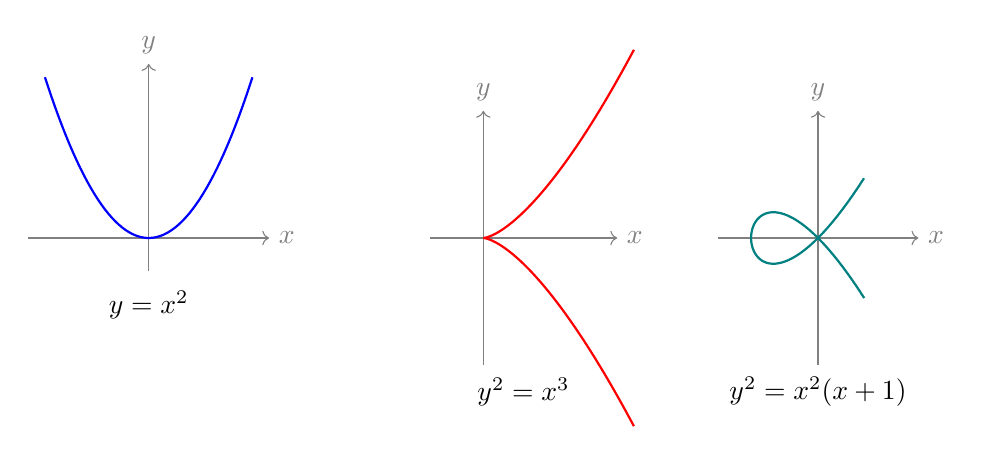
\begin{tikzpicture}[scale=0.85]
  % parabola
  \begin{scope}
    \draw[->,gray] (-1.8,0)--(1.8,0) node[right]{$x$};
    \draw[->,gray] (0,-0.5)--(0,2.6) node[above]{$y$};
    \draw[thick,blue,domain=-1.55:1.55,samples=60] plot (\x,{\x*\x});
    \node at (0,-1) {$y=x^2$};
  \end{scope}
  % cusp
  \begin{scope}[xshift=5cm]
    \draw[->,gray] (-0.8,0)--(2,0) node[right]{$x$};
    \draw[->,gray] (0,-1.9)--(0,1.9) node[above]{$y$};
    \draw[thick,red,domain=0:1.5,samples=60] plot ({\x*\x},{\x*\x*\x/1.2});
    \draw[thick,red,domain=0:1.5,samples=60] plot ({\x*\x},{-\x*\x*\x/1.2});
    \node at (0.6,-2.3) {$y^2=x^3$};
  \end{scope}
  % node
  \begin{scope}[xshift=10cm]
    \draw[->,gray] (-1.5,0)--(1.5,0) node[right]{$x$};
    \draw[->,gray] (0,-1.9)--(0,1.9) node[above]{$y$};
    \draw[thick,teal,domain=-1.3:1.3,samples=80] plot ({\x*\x-1},{\x*(\x*\x-1)});
    \node at (0,-2.3) {$y^2=x^2(x+1)$};
  \end{scope}
\end{tikzpicture}
\caption{$\A^2_\R$ に描いた平面曲線の実点．左から放物線，尖点曲線，結節曲線．}
\label{fig:ch05-curves}
\end{figure}

\subsection{アフィン代数的集合の基本性質}

第3章・第4章で見たように，零点集合をとる操作は次の性質をもつ．

\begin{myprop}{零点集合の基本性質}{ch05-zero-basic}
$S,T\subset k[x_1,\dots,x_n]$，$\{S_\lambda\}_\lambda$ を部分集合の族，$I,J$ をイデアルとする．
\begin{enumerate}
  \item $S\subset T$ ならば $\Zero(T)\subset\Zero(S)$．
  \item $\Zero(I)\cup\Zero(J)=\Zero(IJ)=\Zero(I\cap J)$．
  \item $\bigcap_\lambda \Zero(S_\lambda)=\Zero\bigl(\bigcup_\lambda S_\lambda\bigr)$．
\end{enumerate}
\end{myprop}

\begin{proof}
(1) と (3) は定義から明らか．(2) について，$IJ\subset I\cap J\subset I$ より
$\Zero(I)\cup\Zero(J)\subset\Zero(I\cap J)\subset\Zero(IJ)$．
逆に $p\notin\Zero(I)\cup\Zero(J)$ なら $f(p)\ne0$ なる $f\in I$ と $g(p)\neq 0$ なる $g\in J$ がとれ，
$fg\in IJ$ かつ $(fg)(p)\ne0$ なので $p\notin\Zero(IJ)$．
\end{proof}

したがってアフィン代数的集合の全体は有限和と任意個の共通部分で閉じ，$\emptyset,\A^n$ を含む．
これらを閉集合とする位相が \textbf{Zariski 位相}である（第3章）．
アフィン代数的集合 $X\subset\A^n$ には常に $\A^n$ からの相対位相を入れる．
Zariski 位相は通常の（Euclid）位相よりはるかに粗く，例えば $\A^1$ の真の閉集合は有限集合だけである．
これは「多項式の零点は孤立しているか全体か」という代数の剛性を反映しており，
物理的直感とずれる最初のポイントである．

また $\A^n$ は Noether 位相空間である：閉集合の降鎖 $X_1\supset X_2\supset\cdots$ は必ず停留する．
実際 $\Ideal(X_1)\subset\Ideal(X_2)\subset\cdots$ は Noether 環 $k[x_1,\dots,x_n]$ のイデアルの昇鎖であり停留し，
$X_i=\Zero(\Ideal(X_i))$ だからである．

\subsection{既約アフィン代数的集合}

\begin{mydef}{既約性}{ch05-irred}
空でない位相空間 $X$ が\textbf{既約}であるとは，$X=X_1\cup X_2$（$X_1,X_2$ は閉集合）と書けるならば
$X=X_1$ または $X=X_2$ となることをいう．
\end{mydef}

既約な空間では空でない開集合は必ず稠密であり，空でない開集合どうしは必ず交わる．
Euclid 位相では1点以外の Hausdorff 空間は既約になりえないので，既約性は Zariski 位相特有の概念である．

\begin{myprop}{既約性と素イデアル}{ch05-irred-prime}
アフィン代数的集合 $X\subset \A^n$ が既約であるための必要十分条件は，$\Ideal(X)$ が素イデアルであることである．
\end{myprop}

これは第3章の定理\ref{thm:ch03-irred-prime}の再掲であり，証明もそちらを参照されたい
（要点は，$fg\in\Ideal(X)$ なら $X=(X\cap\Zero(f))\cup(X\cap\Zero(g))$ と閉集合に分解されること）．

Noether 性から次の分解定理が従う．

\begin{mythm}{既約成分分解}{ch05-irred-decomp}
任意のアフィン代数的集合 $X$ は有限個の既約閉集合の和 $X=X_1\cup\cdots\cup X_r$ として書ける．
$i\ne j$ について $X_i\not\subset X_j$ を課せばこの分解は順序を除いて一意であり，各 $X_i$ を $X$ の\textbf{既約成分}という．
\end{mythm}

証明は第3章の定理\ref{thm:ch03-irred-decomp}で与えた（存在は Noether 性による極小反例の議論，一意性は既約性から $X_i\subset Y_j\subset X_l$ となることによる）．

代数的にはこれは根基イデアルの準素分解 $\Ideal(X)=\p_1\cap\cdots\cap\p_r$（$\p_i=\Ideal(X_i)$ は極小素イデアル）に対応する．

\begin{myex}{既約成分}{ch05-components}
$\Zero(xy)\subset\A^2$ は二つの座標軸 $\Zero(x)\cup\Zero(y)$ に分解し，$(xy)=(x)\cap(y)$．
また $\Zero(xz,yz)\subset\A^3$ は $xy$ 平面 $\Zero(z)$ と $z$ 軸 $\Zero(x,y)$ の和であり，
既約成分の次元が異なりうることがわかる．一方，結節曲線 $\Zero(y^2-x^2(x+1))$ は原点で自己交差するが，
$y^2-x^2(x+1)$ は既約多項式なので曲線としては既約である．「見た目に2本の枝がある」ことと「既約成分が2つ」は別の概念である
（枝は局所的な概念であり，第6章・第7章で局所環を用いて扱う）．
\end{myex}

\subsection{アフィン代数的集合と方程式系}

アフィン代数的集合とは，要するに「多項式連立方程式の解集合」である．
ただし同じ解集合が多くの異なる方程式系から得られる点に注意が必要である．例えば
\[
  \Zero(x)=\Zero(x^2)=\Zero(x, xy)\subset \A^2 .
\]
方程式系 $f_1=\cdots=f_r=0$ の情報のうち，解集合 $X$ に依存する部分はイデアル $(f_1,\dots,f_r)$ の根基のみである：
零点定理（第4章）により
\[
  \Ideal(\Zero(f_1,\dots,f_r))=\sqrt{(f_1,\dots,f_r)} .
\]
すなわち
\[
  \{\text{アフィン代数的集合 } X\subset\A^n\}\ \overset{1:1}{\longleftrightarrow}\ \{\text{根基イデアル } I\subset k[x_1,\dots,x_n]\}
\]
であり，この下で既約集合は素イデアルに，点は極大イデアルに対応する．

方程式系を「同値な変形」で書き換えても解集合は変わらない．Gröbner 基底による消去や，変数変換
$x_i\mapsto x_i+(\text{他の変数の多項式})$ はこの意味の書き換えである．
一方，$x=0$ と $x^2=0$ の違い（重複度・無限小の情報）は古典的な代数的集合では失われる．
この情報を保持するのがスキーム論であり，第12章で扱う．

\begin{physbox}[拘束系と代数的集合]
解析力学で，相空間 $T^*Q$ 上の拘束条件 $\phi_a(q,p)=0$ が多項式で与えられるとき，拘束面はアフィン代数的集合である．
Dirac の議論では「弱い等号」$F\approx G$（拘束面上で等しい）が重要であったが，
これはまさに $F-G\in\Ideal(\text{拘束面})$ を意味する．
拘束条件 $\phi_a$ が生成するイデアルが根基でないとき（例えば $\phi=p^2$ のような拘束），
$\phi$ そのものではなく根基の生成元を用いないと拘束面上の関数がうまく記述できない，という
Dirac の「正則性条件」の問題が生じる．これは $\Zero(I)$ と $\sqrt I$ の区別そのものである．
\end{physbox}

\exprob{prob:ch05-1-1}
$X=\Zero(x^2-yz,\ xz-x)\subset\A^3$ の既約成分（問\ref{prob:ch03-9}）それぞれの消滅イデアルを書き，それらの共通部分が $\Ideal(X)$ に等しいことを確かめよ．

\exprob{prob:ch05-1-2}
$\A^1$ の Zariski 位相において，無限部分集合は稠密であることを示せ．また $\A^2$ の Zariski 位相は
$\A^1\times\A^1$ の積位相と一致しないことを示せ．

% ----------------------------------------------------------
\section{アフィン多様体}
% ----------------------------------------------------------

\subsection{アフィン多様体の定義}

\begin{mydef}{アフィン多様体}{ch05-aff-var}
既約なアフィン代数的集合 $X\subset\A^n$ を\textbf{アフィン多様体}という．
同値な言い換えとして，$\Ideal(X)$ が素イデアルであるアフィン代数的集合のことである．
\end{mydef}

\begin{note}
文献によっては既約性を課さず，アフィン代数的集合そのもの（に後述の構造を合わせたもの）をアフィン多様体と呼ぶ．
本ノートでは既約なものをアフィン多様体と呼ぶが，本章の主要な結果（射と環準同型の対応，反変同値）は
既約性を仮定せずに成り立つので，必要に応じて「アフィン代数的集合」の場合も併記する．
\end{note}

「多様体」という言葉に引っ張られて，微分幾何の多様体（局所的に $\R^n$ と同相）を想像してはいけない．
代数多様体は特異点（cusp や node）を許す．特異点を持たない多様体を\emph{非特異}あるいは\emph{滑らか}な多様体と呼び，
第7章で Jacobian 判定法を用いて詳しく調べる．$k=\C$ のとき非特異なアフィン多様体は，
Euclid 位相で複素多様体になる．

\subsection{既約性とアフィン多様体}

なぜ既約性を課すのか．理由は主に次の3点である．
\begin{enumerate}
  \item \textbf{次元が well-defined になる．} 既約成分ごとに次元が異なりうる（例 \ref{ex:ch05-components}）．
        既約ならば次元は「どの点でも同じ」と期待でき，実際そうなる（第7章）．
  \item \textbf{関数体が定まる．} 既約なら座標環 $k[X]$ は整域であり（命題 \ref{prop:ch05-domain}），
        商体 $k(X)=\Frac k[X]$（関数体）がとれる．これは有理写像・双有理幾何（第10章）の基礎である．
  \item \textbf{一致の定理が成り立つ．} 既約な $X$ の上では，空でない開集合上で一致する二つの多項式関数は $X$ 全体で一致する．
\end{enumerate}

(3) を確かめておこう．$U\subset X$ を空でない開集合，$f\in k[X]$ が $U$ 上 $0$ とする．
$X=\Zero_X(f)\cup(X\setminus U)$ は閉集合の和で，$X\setminus U\neq X$ なので既約性から $X=\Zero_X(f)$，すなわち $f=0$．
これは正則（holomorphic）関数に対する一致の定理の類似であり，代数的関数の「剛性」を表している．
滑らかな関数が台をコンパクトにとれる（bump function が存在する）のとは対照的で，第6章の\ref{sec:ch06-phys}節で場の理論の局所性と比較する際に重要になる．

\subsection{アフィン多様体の例}

\begin{myex}{アフィン多様体の例}{ch05-var-examples}
\begin{enumerate}
  \item $\A^n$ 自身：$\Ideal(\A^n)=(0)$ は素イデアル．
  \item 既約多項式 $f$ の定める超曲面 $\Zero(f)$：$k[x_1,\dots,x_n]$ は UFD なので $(f)$ は素イデアル．
        放物線，円（$\mathrm{char}\,k\neq 2$），尖点曲線，結節曲線はいずれもアフィン多様体である．
  \item 線形部分空間（の平行移動）：1次式で生成されるイデアルは素イデアル．
  \item ねじれ3次曲線 $C=\{(t,t^2,t^3)\mid t\in k\}=\Zero(y-x^2,\ z-x^3)\subset\A^3$．
        $k[x,y,z]/(y-x^2,z-x^3)\cong k[x]$ は整域．
  \item $\SL_n=\Zero(\det-1)\subset\A^{n^2}$．$\det-1$ は既約多項式であることが示せる．
  \item 二次錐面 $\Zero(xy-z^2)\subset\A^3$．$xy-z^2$ は既約．
\end{enumerate}
\end{myex}

\begin{myex}{既約でない例}{ch05-nonirr}
$O_2=\{A\in M_2(k)\mid A^{\mathsf T}A=1\}$ を考える．
行列式は $\pm1$ をとり，$O_2=SO_2\sqcup(O_2\cap\Zero(\det+1))$ と二つの既約成分に分解する．
物理でおなじみの「回転」と「反転を含む変換」の2成分であり，Lie 群の連結成分の分解が既約成分分解として現れている．
\end{myex}

\subsection{多様体と代数的集合の関係}

既約成分分解（定理 \ref{thm:ch05-irred-decomp}）により，任意のアフィン代数的集合は有限個のアフィン多様体の和である．
したがって多くの問題は既約な場合に帰着できる．
対応をまとめると次のようになる．
\begin{center}
\renewcommand{\arraystretch}{1.3}
\begin{tabular}{c|c}
幾何 & 代数（$k[x_1,\dots,x_n]$ のイデアル）\\ \hline
アフィン代数的集合 $X$ & 根基イデアル $\Ideal(X)$\\
アフィン多様体（既約） & 素イデアル\\
点 & 極大イデアル\\
既約成分分解 & 極小素イデアルによる表示 $\sqrt I=\p_1\cap\dots\cap\p_r$
\end{tabular}
\end{center}

注意すべきは，この表は $\A^n$ への\emph{埋め込み}を固定した記述だという点である．
放物線 $\Zero(y-x^2)\subset\A^2$ と直線 $\A^1$ は「同じもの」と思いたいが，イデアルは違う環の中にある．
埋め込みに依らない本質的な情報を取り出すのが座標環であり，次節以降の主題である．

\exprob{prob:ch05-2-1}
$X=\Zero(xy-z^2)\subset \A^3$ がアフィン多様体であることを示せ（$xy-z^2$ が既約であることを確かめよ）．
また $X$ の座標環において $\bar z^2=\bar x\bar y$ は $\bar z$ の既約元への分解と $\bar x,\bar y$ への分解を与え，
$k[X]$ は UFD でないことを示せ（$\bar x,\bar y,\bar z$ が $k[X]$ で既約元であることを次数を用いて示してよい）．

% ----------------------------------------------------------
\section{座標環の構成}
% ----------------------------------------------------------

\subsection{多項式関数}

$X\subset \A^n$ をアフィン代数的集合とする．
多項式 $F\in k[x_1,\dots,x_n]$ は写像 $\A^n\to k$ を定めるので，$X$ に制限して関数 $F|_X:X\to k$ が得られる．

\begin{mydef}{多項式関数}{ch05-poly-func}
写像 $f:X\to k$ が\textbf{多項式関数}であるとは，ある $F\in k[x_1,\dots,x_n]$ が存在して $f=F|_X$ となることをいう．
$X$ 上の多項式関数全体を $k[X]$ と書く．
\end{mydef}

$k[X]$ は点ごとの和と積で可換環となり，定数関数を通じて $k$ を含むので $k$ 代数である．
集合 $X$ 上の $k$ 値関数全体のなす $k$ 代数 $\mathrm{Map}(X,k)$ の部分代数であることに注意しよう．
とくに，$k[X]$ の元は「値」によって決まる関数である．
この点が，後に第12章で扱うスキーム（環の元が値だけでは決まらない）との大きな違いである．

物理では「空間上の可観測量（observable）」に相当する．
$X$ が拘束面なら，$k[X]$ は拘束面上の物理量の代数（Dirac 括弧以前の可換代数）である．

\subsection{多項式関数の同値性}

異なる多項式が $X$ 上で同じ関数を定めることがある．例えば放物線 $X=\Zero(y-x^2)$ 上で $y$ と $x^2$ は同じ関数である．
いつ同じになるかは明らかである：
\[
  F|_X=G|_X\iff (F-G)(p)=0\ (\forall p\in X)\iff F-G\in\Ideal(X).
\]
すなわち「$X$ 上で等しい」という同値関係は，イデアル $\Ideal(X)$ を法とする合同関係そのものである．

ここで用いるイデアルが $\Ideal(X)$ であって，$X$ を定義するのに用いた方程式のイデアル $I=(f_1,\dots,f_r)$ ではないことに注意する．
$I\subsetneq \Ideal(X)=\sqrt{I}$ のとき，$I$ を法とする合同は $X$ 上の関数としての等しさよりも細かい．
例えば $X=\Zero(x^2)\subset\A^1$ は原点 $\{0\}$ であり，$x$ は $X$ 上で関数として $0$ だが $x\notin(x^2)$．
（$k[x]/(x^2)$ はいわば「無限小の厚みをもった点」の関数環であり，第12章のスキームで重要な役割を果たす．）

\subsection{座標環の構成}

以上をまとめると次の定理になる．

\begin{myprop}{座標環の表示}{ch05-coord-ring}
制限写像 $\rho: k[x_1,\dots,x_n]\to k[X]$，$F\mapsto F|_X$ は全射な $k$ 代数準同型で，核は $\Ideal(X)$ である．したがって
\[
  k[X]\cong k[x_1,\dots,x_n]/\Ideal(X).
\]
\end{myprop}

\begin{proof}
$\rho$ が $k$ 代数準同型であることは，関数の和・積が点ごとに定義されていることから従う．
全射性は多項式関数の定義そのもの．核が $\Ideal(X)$ であることは前小節で見た．準同型定理より主張を得る．
\end{proof}

\begin{mydef}{座標環}{ch05-coord-ring-def}
$k[X]=k[x_1,\dots,x_n]/\Ideal(X)$ を $X$ の\textbf{座標環}（アフィン座標環）という．
$x_i$ の像を $\bar x_i$ と書き，\textbf{座標関数}と呼ぶ．
\end{mydef}

二つの記述 ―― 「関数のなす環」と「多項式環の商」 ―― は同じものの二つの顔である．
前者は埋め込み $X\subset\A^n$ によらない内在的な記述であり（関数 $X\to k$ の集合として定まる），
後者は計算に便利な具体的表示である．$k[X]$ は $\bar x_1,\dots,\bar x_n$ によって $k$ 代数として生成される．

\begin{figure}[H]
\centering
\begin{tikzcd}[column sep=large,row sep=large]
  k[x_1,\dots,x_n] \arrow[r,"\rho",two heads] \arrow[d,two heads] & k[X]\subset \mathrm{Map}(X,k)\\
  k[x_1,\dots,x_n]/\Ideal(X) \arrow[ru,"\cong"'] &
\end{tikzcd}
\caption{座標環の二つの記述．}
\end{figure}

\subsection{座標環と定義イデアル}

$X=\Zero(I)$ と書いたとき，商環 $k[x_1,\dots,x_n]/I$ と座標環 $k[X]$ の関係は次の通りである．

\begin{myprop}{}{ch05-coord-def-ideal}
$I\subset k[x_1,\dots,x_n]$ をイデアル，$X=\Zero(I)$ とする．自然な全射
\[
  k[x_1,\dots,x_n]/I\twoheadrightarrow k[X]
\]
の核は $\sqrt I/I$，すなわち $k[x_1,\dots,x_n]/I$ の冪零元全体のなすイデアル（冪零根基）である．
とくに，この全射が同型であることと $I$ が根基イデアルであることは同値である．
\end{myprop}

\begin{proof}
零点定理より $\Ideal(X)=\sqrt I$ なので核は $\sqrt I/I$．$\bar F\in k[x]/I$ が冪零 $\iff$ ある $m$ で $F^m\in I$ $\iff F\in\sqrt I$．
\end{proof}

\begin{myex}{定義イデアルが根基でない場合}{ch05-nonrad}
$I=(y^2,\ y-x^2)\subset k[x,y]$ とする．$\Zero(I)$ は放物線と二重直線 $y^2=0$（$x$ 軸）の交わりであり，集合としては原点のみである．
$k[x,y]/I\cong k[x]/(x^4)$ は4次元の $k$ ベクトル空間で，$\bar x$ は冪零．
一方 $k[\Zero(I)]=k[\{0\}]=k$．差の3次元は，放物線が $x$ 軸に原点で接しており（交点重複度 $2$），さらに $x$ 軸を二重に数えている（放物線と二重直線 $y^2=0$ の交点重複度は $2\times2=4$，第9章参照）という情報を担っている．
\end{myex}

\subsection{座標環の具体例}

第4章の例\ref{ex:ch04-coord-examples}で見た例を，同型写像を明示して再確認しておく．

\begin{myex}{座標環の計算}{ch05-coord-examples}
\begin{enumerate}
  \item $k[\A^n]=k[x_1,\dots,x_n]$，$k[\text{点}]=k$．
  \item 放物線 $X=\Zero(y-x^2)$：$k[x,y]/(y-x^2)\to k[t]$，$x\mapsto t$，$y\mapsto t^2$ は同型．よって $k[X]\cong k[t]$．
  \item 双曲線 $H=\Zero(xy-1)$：$k[x,y]/(xy-1)\cong k[t,t^{-1}]$（Laurent 多項式環），$x\mapsto t,\ y\mapsto t^{-1}$．
  \item 尖点曲線 $C=\Zero(y^2-x^3)$：$k[x,y]/(y^2-x^3)\cong k[t^2,t^3]\subset k[t]$．
        実際 $x\mapsto t^2,\ y\mapsto t^3$ は well-defined で，像は $k[t^2,t^3]=\{\sum a_it^i\mid a_1=0\}$．
        単射性は，$k[x,y]/(y^2-x^3)$ の任意の元が $a(x)+b(x)y$ と一意に書け，その像 $a(t^2)+b(t^2)t^3$ は偶数次と奇数次に分かれることから従う．
  \item 二つの座標軸 $X=\Zero(xy)$：$k[X]=k[x,y]/(xy)$．$\bar x\bar y=0$ で $\bar x,\bar y\neq0$ なので零因子をもつ．
  \item 円 $\Zero(x^2+y^2-1)$（$k=\C$）：$u=x+iy,\ v=x-iy$ とおくと $uv=1$ となり，双曲線と同型．$k[X]\cong\C[t,t^{-1}]$．
\end{enumerate}
\end{myex}

(6) は興味深い．実数体上では円（コンパクト）と双曲線（非コンパクト）は全く違うが，複素化すると同じものになる．
複素円 $\{x^2+y^2=1\}\subset\C^2$ は $\C^\times$ と同型であり，実の円 $S^1=U(1)$ は $\C^\times$ の中の $|t|=1$ の部分にすぎない．

\begin{physbox}[$U(1)$ とその複素化]
$U(1)$ の複素化は $\C^\times=\GL_1(\C)$ であり，代数群としては $\Zero(xy-1)\subset\A^2$，座標環は $\C[t,t^{-1}]$ である．
$U(1)$ の既約表現 $e^{in\theta}$（$n\in\Z$）が座標環の基底 $t^n$ に対応している．
Fourier 級数の「三角多項式」の環は，まさにこの座標環である．
一般に，コンパクト Lie 群 $G$ の複素化 $G_\C$ は代数群（アフィン多様体）となり，その座標環 $\C[G_\C]$ は
Peter--Weyl の定理により $\bigoplus_{V}V^*\otimes V$（$V$ は既約表現）と分解する．
\end{physbox}

\exprob{prob:ch05-3-1}
ねじれ3次曲線 $C=\Zero(y-x^2,\ z-x^3)\subset\A^3$ を考える（$k[C]\cong k[t]$ は問\ref{prob:ch04-8}で示した）．
$J=(xz-y^2,\ y-x^2)$ とするとき，$\Zero(J)$ を既約分解し，$\Zero(J)\supsetneq C$ であること（したがって $J\ne\Ideal(C)$）を示せ．
また $C$ を切り出すには $xz-y^2,\ y-x^2$ にどのような方程式を追加すればよいか答えよ．

% ----------------------------------------------------------
\section{座標環の性質}
% ----------------------------------------------------------

\subsection{座標環の有限生成性}

\begin{myprop}{座標環は有限生成被約 $k$ 代数}{ch05-fg-reduced}
アフィン代数的集合 $X$ の座標環 $k[X]$ は次を満たす．
\begin{enumerate}
  \item $k$ 代数として有限生成である．
  \item 被約である，すなわち $0$ 以外の冪零元をもたない．
\end{enumerate}
逆に，有限生成被約 $k$ 代数 $A$ は，あるアフィン代数的集合 $X$ の座標環と $k$ 代数として同型である．
\end{myprop}

\begin{proof}
(1) $k[X]$ は座標関数 $\bar x_1,\dots,\bar x_n$ で生成される．
(2) $f\in k[X]$ が $f^m=0$ を満たせば，各点 $p$ で $f(p)^m=0$，体 $k$ は整域なので $f(p)=0$．よって $f=0$．
（イデアルの言葉では，$\Ideal(X)$ が根基イデアルであることと同じである．）

逆に $A$ が $a_1,\dots,a_n$ で生成されるとすると，全射 $\pi:k[x_1,\dots,x_n]\to A$，$x_i\mapsto a_i$ がある．
$I=\Ker\pi$ とおけば $A\cong k[x_1,\dots,x_n]/I$．$A$ が被約であることは $I$ が根基であることと同値である
（$F^m\in I\Rightarrow \pi(F)^m=0\Rightarrow\pi(F)=0\Rightarrow F\in I$）．
$X=\Zero(I)$ とすれば零点定理より $\Ideal(X)=\sqrt I=I$，よって $k[X]\cong A$．
\end{proof}

この命題の後半で，零点定理（$k$ が代数閉体であること）が本質的に使われている．
例えば $k=\R$ で $A=\R[x]/(x^2+1)\cong\C$ は有限生成被約 $\R$ 代数だが，$\Zero_\R(x^2+1)=\emptyset$ であり，
実点の上の関数環としては実現できない．

$A$ の生成元のとり方は一意ではない．生成元を変えると $X$ は別の $\A^m$ の中に実現されるが，
後で見るように（\ref{sec:ch05-ring-geom} 節）それらはすべて互いに同型な多様体である．

\subsection{座標環と整域}

\begin{myprop}{既約 $\iff$ 座標環が整域}{ch05-domain}
アフィン代数的集合 $X$ について次は同値である．
\begin{enumerate}
  \item $X$ は既約である（すなわちアフィン多様体である）．
  \item $\Ideal(X)$ は素イデアルである．
  \item $k[X]$ は整域である．
\end{enumerate}
\end{myprop}

\begin{proof}
(1)$\iff$(2) は命題 \ref{prop:ch05-irred-prime}．(2)$\iff$(3) は「$R/\p$ が整域 $\iff$ $\p$ が素イデアル」という一般論である．
\end{proof}

(3) の幾何的意味を直接見ておくと理解が深まる．$X=X_1\cup X_2$ が真の分解なら，
$f$ を「$X_1$ 上で $0$，$X_2$ 上で $0$ でない」関数，$g$ をその逆とすると，$fg=0$ だが $f,g\ne0$ である．
座標軸 $\Zero(xy)$ では $f=\bar x$，$g=\bar y$ がそれである（図 \ref{fig:ch05-zero-div}）．
零因子は「別々の成分に台をもつ関数」の存在を意味する．

\begin{figure}[H]
\centering
\begin{tikzpicture}[scale=0.9]
  \draw[very thick,blue] (-2,0)--(2,0) node[right]{$\Zero(y)$：ここで $\bar y=0$};
  \draw[very thick,red] (0,-1.5)--(0,1.5) node[above]{$\Zero(x)$：ここで $\bar x=0$};
  \fill (0,0) circle (2pt);
\end{tikzpicture}
\caption{$\Zero(xy)$ 上で $\bar x\bar y=0$ だが $\bar x,\bar y\neq0$．}
\label{fig:ch05-zero-div}
\end{figure}

\subsection{座標環と既約性}

以上から，\emph{アフィン多様体の座標環は有限生成な整域 $k$ 代数}であり，逆に有限生成整域 $k$ 代数はアフィン多様体の座標環である．
既約成分分解は座標環の言葉では次のように表される．
$X=X_1\cup\cdots\cup X_r$ を既約成分分解，$\p_i=\Ideal(X_i)/\Ideal(X)\subset k[X]$ とすると，
$\p_1,\dots,\p_r$ はちょうど $k[X]$ の極小素イデアルであり，
\[
  \p_1\cap\cdots\cap\p_r=0,\qquad k[X]\hookrightarrow \prod_{i=1}^r k[X_i]
\]
が成り立つ（$f\mapsto(f|_{X_1},\dots,f|_{X_r})$ が単射であることは明らか）．
ただしこれは一般には全射ではない：$X=\Zero(xy)$ では $k[X]\to k[x]\times k[y]$ の像は
$\{(a(x),b(y))\mid a(0)=b(0)\}$ であり，「二つの成分が原点で貼り合わされている」ことを表している．
既約成分が交わらない場合に限りこの写像は同型になる（中国剰余定理）．

\subsection{座標環による幾何学的情報の表現}

座標環には $X$ の幾何学的情報がすべて含まれている．第4章で見た対応を $k[X]$ の言葉で言い直すと：

\begin{myprop}{座標環のイデアルと $X$ の部分集合}{ch05-ideal-corr}
アフィン代数的集合 $X$ に対し，$J\subset k[X]$ をイデアルとして $\Zero_X(J)=\{p\in X\mid f(p)=0\ \forall f\in J\}$，
$Y\subset X$ に対し $\Ideal_X(Y)=\{f\in k[X]\mid f|_Y=0\}$ とおく．このとき
\[
  \{X\text{ の閉部分集合}\}\overset{1:1}{\longleftrightarrow}\{k[X]\text{ の根基イデアル}\}
\]
であり，既約閉部分集合は素イデアルに，点は極大イデアルに対応する．
点 $p\in X$ に対応する極大イデアルは $\m_p=\{f\in k[X]\mid f(p)=0\}$ であり，$k[X]/\m_p\cong k$（$f\mapsto f(p)$）．
\end{myprop}

\begin{proof}[証明の概略]
$k[X]=k[x]/\Ideal(X)$ のイデアルは $\Ideal(X)$ を含む $k[x]$ のイデアルと一対一に対応し，この対応は根基性・素性・極大性を保つ．
あとは $\A^n$ での対応（第4章）を $X$ に制限すればよい．
\end{proof}

すなわち $X$ は集合として $k[X]$ の極大イデアル全体 $\mathrm{Max}\,k[X]$ と同一視でき，
Zariski 位相も $k[X]$ から復元できる．関数 $f\in k[X]$ の点 $p$ での値は「$f$ の $k[X]/\m_p\cong k$ での像」である．
こうして\emph{空間 $X$ を忘れて環 $k[X]$ だけから $X$ を再構成できる}．
極大イデアルだけでなく素イデアル全体を点とみなすのが $\Spec$ であり，第12章で導入する．

\begin{physbox}[状態と可観測量]
量子力学・古典力学のいずれでも，「状態」は可観測量の代数 $\mathcal A$ 上の線形汎関数（期待値）$\omega:\mathcal A\to\C$ として捉えられる．
古典系の純粋状態（相空間の点 $p$）は，$f\mapsto f(p)$ という\emph{乗法的}な汎関数，すなわち代数準同型 $\mathcal A\to\C$ である．
その核は極大イデアル $\m_p$ にほかならない．
「点 $=$ 評価準同型 $=$ 極大イデアル」という対応は，可換 $C^*$ 代数に対する Gelfand--Naimark の定理と同じ構図であり，
座標環からの多様体の再構成はその代数幾何版とみなせる．
\end{physbox}

\exprob{prob:ch05-4-1}
$A=k[x,y]/(x^2,xy)$ は有限生成 $k$ 代数であるが被約ではないことを示し，その冪零根基を求めよ．
また $\Zero(x^2,xy)\subset\A^2$ の座標環を求めよ．

% ----------------------------------------------------------
\section{多様体間の写像}
% ----------------------------------------------------------

\subsection{多様体間の写像}

幾何学では対象だけでなく，対象の間の「構造を保つ写像」が重要である．
位相空間なら連続写像，微分多様体なら $C^\infty$ 写像，複素多様体なら正則写像であった．
代数幾何学における自然な写像のクラスは「座標が多項式（あるいは局所的に有理式）で書ける写像」である．
本節ではアフィン代数的集合の間でこれを定義し，同型・閉埋め込みを導入する．
射の一般論（準射影多様体の間の射，合成，有理写像との違い）は第10章で扱う．

\subsection{多項式写像}

\begin{mydef}{多項式写像}{ch05-poly-map}
$X\subset\A^n$，$Y\subset\A^m$ をアフィン代数的集合とする．写像 $\varphi:X\to Y$ が\textbf{多項式写像}であるとは，
多項式 $F_1,\dots,F_m\in k[x_1,\dots,x_n]$ が存在して
\[
  \varphi(p)=(F_1(p),\dots,F_m(p))\qquad(p\in X)
\]
となることをいう．言い換えれば，各成分 $\varphi_j=y_j\circ\varphi$ が $X$ 上の多項式関数 $\in k[X]$ であることである．
\end{mydef}

成分 $F_j$ は $\Ideal(X)$ を法としてのみ決まる．また $\varphi$ の像が $Y$ に入るという条件は，
任意の $G\in\Ideal(Y)$ に対して $G(F_1,\dots,F_m)\in\Ideal(X)$ となることと同値である．

\begin{myex}{多項式写像の例}{ch05-polymap-ex}
\begin{enumerate}
  \item 射影 $\pi:\A^2\to\A^1$，$(x,y)\mapsto x$．放物線や双曲線に制限すると $\Zero(y-x^2)\to\A^1$，$\Zero(xy-1)\to\A^1$ を得る．
  \item パラメータ表示 $\A^1\to\Zero(y^2-x^3)$，$t\mapsto(t^2,t^3)$．$(t^3)^2-(t^2)^3=0$ なので像は尖点曲線に入る．
  \item 行列の積 $M_n\times M_n\to M_n$，行列式 $\det:M_n\to\A^1$，群演算 $\SL_n\times\SL_n\to\SL_n$．
  \item $k=\F_q$ の代数閉包上の Frobenius 写像 $(x_1,\dots,x_n)\mapsto(x_1^q,\dots,x_n^q)$（正標数特有の重要な例）．
\end{enumerate}
\end{myex}

多項式写像 $\varphi:X\to Y$ は Zariski 位相について連続である．実際，閉集合 $Z=\Zero_Y(G_1,\dots,G_s)$ の逆像は
$\varphi^{-1}(Z)=\Zero_X(G_1\circ\varphi,\dots,G_s\circ\varphi)$ であり閉集合である．

\subsection{正則写像}

多項式写像はアフィン空間への埋め込みを用いて定義した．
埋め込みに依らない定義を与え，さらに後の章で開集合（アフィンとは限らない）を扱えるようにするために，
「局所的に有理式で書ける」という正則性の概念を導入する．

\begin{mydef}{正則関数}{ch05-regular-func}
$X$ をアフィン多様体，$U\subset X$ を開集合とする．関数 $f:U\to k$ が点 $p\in U$ で\textbf{正則}であるとは，
$p$ の開近傍 $V\subset U$ と $g,h\in k[X]$ が存在して，$V$ 上で $h\neq 0$ かつ $f=g/h$ となることをいう．
$U$ のすべての点で正則なとき $f$ は $U$ 上正則であるといい，その全体を $\OO_X(U)$ と書く．
\end{mydef}

分母 $h$ は点ごとに取り替えてよいことに注意する．多項式関数は明らかに正則である．
基本的な事実は，大域的には逆も成り立つことである．

\begin{mythm}{大域正則関数}{ch05-global-regular}
アフィン多様体 $X$ について $\OO_X(X)=k[X]$．
\end{mythm}

\begin{proof}
$f\in\OO_X(X)$ とする．$k[X]$ は整域なので商体 $k(X)$ がとれる．
各点 $p$ の近傍 $V_p$ で $f=g_p/h_p$ と書けるとき，$V_p\cap V_q$ 上で $g_ph_q=g_qh_p$ であり，
$V_p\cap V_q$ は空でない開集合（既約性）なので一致の定理より $k[X]$ において $g_ph_q=g_qh_p$．
したがって $f$ は $k(X)$ の元 $g_p/h_p$（$p$ によらない）とみなせる．そこで
\[
  J=\{h\in k[X]\mid hf\in k[X]\}
\]
とおくと $J$ は $k[X]$ のイデアルで，すべての $p$ について $h_p\in J$ かつ $h_p(p)\ne0$．
よって $\Zero_X(J)=\emptyset$ であり，零点定理（命題 \ref{prop:ch05-ideal-corr}）より $J=k[X]$，すなわち $1\in J$，$f\in k[X]$．
\end{proof}

この定理の証明に見られる「分母のイデアルを考えて零点定理で $1$ を含むことを示す」という論法は，
第6章で局所化を用いて系統的に扱われる（$\OO_X(X)=\bigcap_{p}\OO_{X,p}$）．

\begin{mydef}{正則写像（射）}{ch05-morphism}
$X\subset\A^n$，$Y\subset\A^m$ をアフィン多様体とする．写像 $\varphi:X\to Y$ が\textbf{正則写像}（あるいは\textbf{射}）であるとは，
$\varphi$ が連続であり，任意の開集合 $V\subset Y$ と $f\in\OO_Y(V)$ に対して $f\circ\varphi\in\OO_X(\varphi^{-1}(V))$ となることをいう．
\end{mydef}

\begin{myprop}{射 $=$ 多項式写像}{ch05-reg-eq-poly}
アフィン多様体の間の写像 $\varphi:X\to Y\subset\A^m$ について，次は同値である．
\begin{enumerate}
  \item $\varphi$ は正則写像である．
  \item 各成分 $\varphi_j=y_j\circ\varphi$ は $X$ 上の正則関数である．
  \item $\varphi$ は多項式写像である．
\end{enumerate}
\end{myprop}

\begin{proof}
(1)$\Rightarrow$(2)：座標関数 $\bar y_j\in k[Y]=\OO_Y(Y)$ を引き戻せばよい．
(2)$\Rightarrow$(3)：定理 \ref{thm:ch05-global-regular} より $\varphi_j\in k[X]$．
(3)$\Rightarrow$(1)：多項式写像は連続である．$f\in\OO_Y(V)$ が $q=\varphi(p)$ の近傍で $g/h$（$g,h\in k[Y]$）と書けるなら，
$f\circ\varphi$ は $p$ の近傍で $(g\circ\varphi)/(h\circ\varphi)$ と書け，$g\circ\varphi,h\circ\varphi\in k[X]$ である．
\end{proof}

したがってアフィン多様体の間では「正則写像」「射」「多項式写像」は同じものである．
正則関数の概念が真価を発揮するのは，開集合 $U\subset X$ や射影多様体を扱うときであり，それは構造層 $\OO_X$ として第11章で定式化される．
（既約でないアフィン代数的集合に対しても，「射 $=$ 多項式写像」と定義すれば以下の議論はそのまま成り立つ．）

\subsection{多様体の同型}

\begin{mydef}{同型}{ch05-iso}
射 $\varphi:X\to Y$ が\textbf{同型}であるとは，射 $\psi:Y\to X$ で $\psi\circ\varphi=\mathrm{id}_X$，$\varphi\circ\psi=\mathrm{id}_Y$ を満たすものが存在することをいう．
このとき $X\cong Y$ と書く．
\end{mydef}

同型は全単射な射であるが，\emph{逆写像も射であること}を要求している点が肝心である．
これは微分幾何で「全単射な $C^\infty$ 写像は微分同相とは限らない（例：$x\mapsto x^3$）」のと同様である．

\begin{myex}{放物線 $\cong\A^1$}{ch05-parabola}
$\varphi:\A^1\to X=\Zero(y-x^2)$，$t\mapsto(t,t^2)$ と $\psi:X\to\A^1$，$(x,y)\mapsto x$ は互いに逆の射である．
よって $X\cong\A^1$．グラフ $\{y=f(x)\}$ は一般に $\A^1$ と同型である．
\end{myex}

\begin{myex}{$\A^1\setminus\{0\}\cong \Zero(xy-1)$}{ch05-punctured}
$\A^1\setminus\{0\}$ は $\A^1$ の開集合であり，それ自身は $\A^1$ の閉集合ではない．
しかし射影 $\pi:H=\Zero(xy-1)\to\A^1$，$(x,y)\mapsto x$ は $H$ から $\A^1\setminus\{0\}$ への全単射で，
逆写像 $x\mapsto(x,1/x)$ は $\A^1\setminus\{0\}$ 上の正則関数で書ける．
したがって $\A^1\setminus\{0\}$ は（正則関数の構造まで込めて）アフィン多様体 $H$ と同型であり，その正則関数環は
\[
  \OO(\A^1\setminus\{0\})\cong k[H]=k[x,y]/(xy-1)\cong k[x,x^{-1}].
\]
「$x$ で割ることを許す」操作が，「新しい変数 $y$ と方程式 $xy=1$ を付け加える」ことで実現されている（Rabinowitsch のトリック）．
これは第6章の局所化 $k[x]_x=k[x,x^{-1}]$ の最初の例である．
\end{myex}

\begin{figure}[H]
\centering
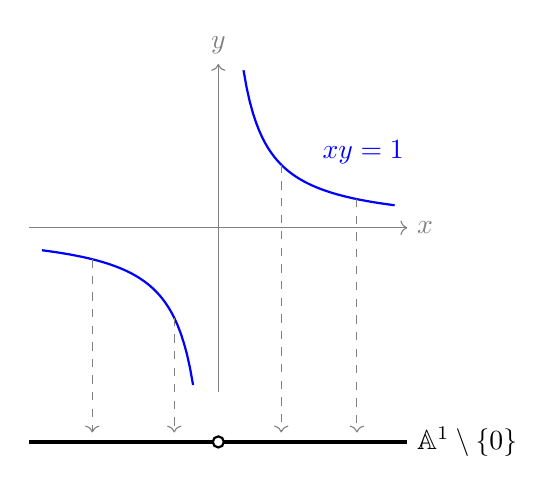
\begin{tikzpicture}[scale=0.8]
  \draw[->,gray] (-3,0)--(3,0) node[right]{$x$};
  \draw[->,gray] (0,-2.6)--(0,2.6) node[above]{$y$};
  \draw[thick,blue,domain=0.4:2.8,samples=50] plot (\x,{1/\x});
  \draw[thick,blue,domain=-2.8:-0.4,samples=50] plot (\x,{1/\x});
  \node[blue] at (2.3,1.2) {$xy=1$};
  \draw[very thick] (-3,-3.4)--(-0.07,-3.4);
  \draw[very thick] (0.07,-3.4)--(3,-3.4);
  \draw[thick,fill=white] (0,-3.4) circle (2.5pt);
  \node[right] at (3,-3.4) {$\A^1\setminus\{0\}$};
  \foreach \t in {-2,-0.7,1,2.2}{
    \draw[dashed,->,gray] (\t,{1/\t}) -- (\t,-3.25);
  }
\end{tikzpicture}
\caption{双曲線 $\Zero(xy-1)$ の $x$ 軸への射影は $\A^1\setminus\{0\}$ への同型．}
\label{fig:ch05-hyperbola}
\end{figure}

\begin{note}
すべての開集合がアフィンになるわけではない．例えば $\A^2\setminus\{0\}$ 上の正則関数は $k[x,y]$ に一致する（Hartogs 現象の代数版）ので，
もしアフィンなら $\A^2$ と同型になってしまうが，$\A^2\setminus\{0\}\to\A^2$ は全射でないので矛盾する．
\end{note}

\begin{myex}{尖点曲線：同相だが同型でない}{ch05-cusp}
$C=\Zero(y^2-x^3)$ とし，$\varphi:\A^1\to C$，$t\mapsto(t^2,t^3)$ を考える．
\begin{itemize}
  \item \textbf{全単射：} $(x,y)\in C$ で $x\neq0$ なら $t=y/x$ が唯一の逆像（$t^2=y^2/x^2=x$，$t^3=x t=y$），$x=0$ なら $y=0$ で $t=0$．
  \item \textbf{同相：} $\A^1$ と $C$ はともに既約な曲線であり，真の閉集合は有限集合のみである．全単射は有限集合を有限集合に移すので，$\varphi$ も $\varphi^{-1}$ も連続である．
  \item \textbf{同型でない：} 逆写像は $(x,y)\mapsto y/x$（$x\ne 0$），$(0,0)\mapsto0$ で与えられるが，これは多項式で書けない．
        実際，もし $\psi:C\to\A^1$ が射で $\psi\circ\varphi=\mathrm{id}$ なら，$\psi=G(\bar x,\bar y)$ として $G(t^2,t^3)=t$．
        しかし $G(t^2,t^3)\in k[t^2,t^3]$ は $t$ の1次の項をもたない（例 \ref{ex:ch05-coord-examples} (4)）ので矛盾する．
\end{itemize}
代数的には，$\varphi^*:k[C]\to k[\A^1]=k[t]$ の像が $k[t^2,t^3]\subsetneq k[t]$ で全射でないことが原因である．
幾何学的には，$C$ は原点に特異点をもつ（原点での接空間が2次元になる，第7章）のに対し $\A^1$ は滑らかである．
同相写像であっても局所的な代数構造（局所環，第6章）までは保たない．
\end{myex}

\begin{figure}[H]
\centering
\begin{tikzpicture}[scale=0.85]
  \draw[very thick] (-2.2,0)--(2.2,0) node[right]{$\A^1$};
  \foreach \t/\c in {-1.4/red,-0.7/orange,0/black,0.7/teal,1.4/blue}{\fill[\c] (\t,0) circle (2pt);}
  \draw[->,thick] (2.9,0)--(4.4,0) node[midway,above]{$t\mapsto(t^2,t^3)$};
  \begin{scope}[xshift=5.4cm]
    \draw[->,gray] (-0.5,0)--(2.6,0);
    \draw[->,gray] (0,-2)--(0,2);
    \draw[thick,red!70!black,domain=0:1.5,samples=60] plot ({\x*\x},{\x*\x*\x/1.2});
    \draw[thick,red!70!black,domain=0:1.5,samples=60] plot ({\x*\x},{-\x*\x*\x/1.2});
    \foreach \t/\c in {-1.4/red,-0.7/orange,0/black,0.7/teal,1.4/blue}{
      \fill[\c] ({\t*\t},{\t*\t*\t/1.2}) circle (2pt);}
    \node at (1.5,-2.3) {$C=\Zero(y^2-x^3)$};
  \end{scope}
\end{tikzpicture}
\caption{$\A^1$ から尖点曲線への全単射．逆写像は原点で多項式にならない．}
\label{fig:ch05-cusp}
\end{figure}

\subsection{多様体の埋め込み}

\begin{mydef}{閉埋め込み}{ch05-closed-emb}
射 $\varphi:X\to Y$ が\textbf{閉埋め込み}であるとは，像 $Z=\varphi(X)$ が $Y$ の閉集合であり，
$\varphi$ が $X$ から $Z$（閉部分多様体としての構造）への同型を与えることをいう．
\end{mydef}

\begin{myprop}{閉埋め込みの代数的判定}{ch05-closed-emb-crit}
アフィン代数的集合の射 $\varphi:X\to Y$ が閉埋め込みであるための必要十分条件は，$\varphi^*:k[Y]\to k[X]$，$g\mapsto g\circ\varphi$ が全射であることである．
\end{myprop}

\begin{proof}[証明の概略]
閉埋め込みなら $\varphi^*$ は制限写像 $k[Y]\to k[Z]$ と同型 $k[Z]\cong k[X]$ の合成であり，前者は全射（命題 \ref{prop:ch05-coord-ring} と同じ理由）．
逆に $\varphi^*$ が全射で核を $J$ とすると $k[X]\cong k[Y]/J$．$Z=\Zero_Y(J)$ とすると $k[Z]=k[Y]/\sqrt J=k[Y]/J$（$k[Y]/J\cong k[X]$ が被約なので $J$ は根基）．
次節の定理 \ref{thm:ch05-equiv} により，この $k$ 代数同型 $k[Z]\cong k[X]$ は同型 $X\cong Z$ から来ており，それが $\varphi$ と一致する．
\end{proof}

とくに，アフィン代数的集合 $X$ を座標環の生成元 $f_1,\dots,f_m$ を用いて写した $X\to\A^m$，$p\mapsto(f_1(p),\dots,f_m(p))$ は閉埋め込みである
（$k[y_1,\dots,y_m]\to k[X]$，$y_j\mapsto f_j$ が全射だから）．アフィン代数的集合とは「アフィン空間に閉埋め込みできる空間」であり，
埋め込み方は生成元の選び方だけある．

\begin{myex}{埋め込みの例}{ch05-emb-ex}
\begin{enumerate}
  \item $\A^1\to\A^3$，$t\mapsto(t,t^2,t^3)$ はねじれ3次曲線への閉埋め込み．$\varphi^*(x)=t$ なので全射．
  \item 射 $\varphi:X\to Y$ のグラフ $\Gamma_\varphi=\{(p,\varphi(p))\}\subset X\times Y$ への写像 $p\mapsto(p,\varphi(p))$ は閉埋め込み．
  \item 尖点曲線への $\varphi:\A^1\to C\subset\A^2$ は単射かつ像は閉だが，閉埋め込みではない（$\varphi^*$ が全射でない）．
  \item $\A^1\to\A^2$，$t\mapsto(t^2-1,\ t(t^2-1))$ は結節曲線 $\Zero(y^2-x^2(x+1))$ への全射だが，$t=\pm1$ が同じ点に移り単射でない．
\end{enumerate}
\end{myex}

\begin{physbox}[埋め込みとパラメータ表示]
物理では空間を「パラメータで表示する」（$\A^1\to C$）ことと「拘束条件で切り出す」（$C=\Zero(f)\subset\A^2$）ことの両方がよく用いられる．
前者は射 $\A^1\to C$，後者は閉埋め込み $C\hookrightarrow\A^2$ である．
尖点曲線の例は，パラメータ表示が全単射でも「良い座標」になっていないことがあることを示している．
例えば $t$ を時間とする粒子の軌道 $(x,y)=(t^2,t^3)$ は $t=0$ で速度が $0$ になって軌道が尖る．
曲線上の関数としては $t=y/x$ は滑らかに見えても，原点では多項式（あるいは正則関数）として表せない．
\end{physbox}

\exprob{prob:ch05-5-1}
$\varphi:\A^1\to\A^2$，$t\mapsto(t^2,t^5)$ の像を定める多項式を求め，$\varphi$ が像への同相写像であるが同型ではないことを示せ．

\exprob{prob:ch05-5-2}
$k=\C$ とする．$\A^1$ から $\A^1$ への同型はすべて $t\mapsto at+b$（$a\neq0$）の形であることを示せ．
また $\Zero(xy-1)$ の自己同型をすべて求めよ．

% ----------------------------------------------------------
\section{幾何学と環論の対応}
\label{sec:ch05-ring-geom}
% ----------------------------------------------------------

\subsection{多様体の射と環準同型}

射 $\varphi:X\to Y$ が与えられると，関数の引き戻し
\[
  \varphi^*:k[Y]\to k[X],\qquad \varphi^*(g)=g\circ\varphi
\]
が定まる．$g\in k[Y]$ が多項式 $G(y_1,\dots,y_m)$ の制限なら $g\circ\varphi$ は $G(F_1,\dots,F_m)$ の制限であって $k[X]$ に属し，
$\varphi^*$ が $k$ 代数準同型であること（和・積・定数を保つこと）は明らかである．
本章の中心定理は，逆にすべての $k$ 代数準同型がこのようにして得られることである．

\begin{mythm}{射と $k$ 代数準同型の対応}{ch05-morph-hom}
$X,Y$ をアフィン代数的集合とする．写像
\[
  \Hom(X,Y)\longrightarrow\Hom_{k\text{-alg}}(k[Y],k[X]),\qquad \varphi\longmapsto\varphi^*
\]
は全単射である．
\end{mythm}

\begin{proof}
$Y\subset\A^m$ とし，$k[Y]=k[y_1,\dots,y_m]/\Ideal(Y)$，$\bar y_j$ を座標関数とする．

\textbf{単射性．} $\varphi,\psi:X\to Y$ が $\varphi^*=\psi^*$ を満たすとする．各 $j$ について
$\bar y_j\circ\varphi=\varphi^*(\bar y_j)=\psi^*(\bar y_j)=\bar y_j\circ\psi$．
点 $\varphi(p)\in Y\subset\A^m$ はその座標 $(\bar y_1(\varphi(p)),\dots,\bar y_m(\varphi(p)))$ で決まるので $\varphi=\psi$．

\textbf{全射性．} $k$ 代数準同型 $u:k[Y]\to k[X]$ が与えられたとする．$f_j=u(\bar y_j)\in k[X]$ とおき
\[
  \varphi:X\to\A^m,\qquad \varphi(p)=(f_1(p),\dots,f_m(p))
\]
と定める．これは多項式写像である．像が $Y$ に含まれることを示す．$G\in\Ideal(Y)$ とすると，$u$ は $k$ 代数準同型なので
\[
  G(f_1,\dots,f_m)=G(u(\bar y_1),\dots,u(\bar y_m))=u\bigl(G(\bar y_1,\dots,\bar y_m)\bigr)=u(0)=0\quad(\text{in }k[X])．
\]
よって任意の $p\in X$ で $G(\varphi(p))=G(f_1,\dots,f_m)(p)=0$，すなわち $\varphi(p)\in\Zero(\Ideal(Y))=Y$．
こうして射 $\varphi:X\to Y$ を得た．最後に $\varphi^*=u$ を確かめる．
$\varphi^*(\bar y_j)=\bar y_j\circ\varphi=f_j=u(\bar y_j)$ であり，$k[Y]$ は $\bar y_j$ たちで $k$ 代数として生成されるので，
二つの $k$ 代数準同型 $\varphi^*$ と $u$ は一致する．
\end{proof}

証明の要点は，「$k[Y]$ からの準同型は生成元 $\bar y_j$ の行き先で決まり，行き先は関係式 $\Ideal(Y)$ を満たしさえすればよい」という商環の普遍性と，
「$X$ の点は $\Zero(\Ideal(Y))$ に入るかどうかで $Y$ の点か判定できる」という零点定理の帰結
（$Y=\Zero(\Ideal(Y))$）を組み合わせたことである．

\begin{myex}{対応の具体例}{ch05-morph-hom-ex}
\begin{enumerate}
  \item 点 $p:\{\mathrm{pt}\}\to X$ は $k[X]\to k[\mathrm{pt}]=k$，すなわち評価写像 $f\mapsto f(p)$ に対応する．
        よって $X\cong \Hom_{k\text{-alg}}(k[X],k)$．これは命題 \ref{prop:ch05-ideal-corr} の言い換えである（核が $\m_p$）．
  \item 射 $X\to\A^1$ は $k[t]\to k[X]$，すなわち $t$ の行き先 $f\in k[X]$ で決まる．よって $\Hom(X,\A^1)=k[X]$：
        \emph{座標環の元とは $\A^1$ への射のことである．}
  \item 尖点曲線のパラメータ表示 $\A^1\to C$ は $k[x,y]/(y^2-x^3)\to k[t]$，$x\mapsto t^2$，$y\mapsto t^3$ に対応する．
  \item 射影 $\Zero(xy-1)\to\A^1$ は包含 $k[x]\hookrightarrow k[x,x^{-1}]$ に対応する．
\end{enumerate}
\end{myex}

\subsection{反変性}

対応 $\varphi\mapsto\varphi^*$ は合成と整合的であるが，\emph{向きを逆にする}．
射 $X\xrightarrow{\varphi}Y\xrightarrow{\psi}Z$ に対して，$h\in k[Z]$ について
$(\psi\circ\varphi)^*(h)=h\circ\psi\circ\varphi=\varphi^*(\psi^*(h))$ なので
\[
  (\psi\circ\varphi)^*=\varphi^*\circ\psi^*,\qquad (\mathrm{id}_X)^*=\mathrm{id}_{k[X]}.
\]

\begin{figure}[H]
\centering
\begin{tikzcd}[column sep=large,row sep=large]
  X \arrow[r,"\varphi"] \arrow[rr,bend left=30,"\psi\circ\varphi"] & Y \arrow[r,"\psi"] & Z\\
  k[X] & k[Y] \arrow[l,"\varphi^*"'] & k[Z] \arrow[l,"\psi^*"'] \arrow[ll,bend left=30,"\varphi^*\circ\psi^*"]
\end{tikzcd}
\caption{座標環をとる操作は矢印の向きを逆にする（反変関手）．}
\end{figure}

この反変性から直ちに次がわかる．

\begin{mycor}{同型の判定}{ch05-iso-crit}
アフィン代数的集合 $X,Y$ について，$X\cong Y$ であることと $k[X]\cong k[Y]$（$k$ 代数として）であることは同値である．
より詳しく，射 $\varphi$ が同型であることと $\varphi^*$ が同型であることは同値である．
\end{mycor}

\begin{proof}
$\psi\circ\varphi=\mathrm{id}$，$\varphi\circ\psi=\mathrm{id}$ は $\varphi^*\circ\psi^*=\mathrm{id}$，$\psi^*\circ\varphi^*=\mathrm{id}$ と同値（定理 \ref{thm:ch05-morph-hom} の全単射性）．
また任意の $k$ 代数同型 $k[Y]\to k[X]$ はある射の引き戻しである．
\end{proof}

この系により，尖点曲線 $C$ と $\A^1$ が同型でないことは「$k[t^2,t^3]\not\cong k[t]$」に帰着される．
後者は例えば，$k[t]$ が整閉（UFD）であるのに $k[t^2,t^3]$ では $t=t^3/t^2$ が商体の元として整（$t^2-\bar x=0$ の根）だが環に属さない，ことから分かる．

圏論の言葉でまとめよう（圏論的視点の一般論は第10章で改めて扱う）．

\begin{mythm}{アフィン代数的集合と $k$ 代数の反変同値}{ch05-equiv}
関手
\[
  \left\{\begin{array}{c}\text{アフィン代数的集合}\\ \text{と射}\end{array}\right\}
  \longrightarrow
  \left\{\begin{array}{c}\text{有限生成被約 } k \text{ 代数}\\ \text{と } k \text{ 代数準同型}\end{array}\right\}^{\mathrm{op}}
\]
（$X\mapsto k[X]$，$\varphi\mapsto\varphi^*$）は圏同値である．この同値はアフィン多様体（既約）の圏と有限生成整域 $k$ 代数の圏の反対圏との同値に制限される．
\end{mythm}

\begin{proof}
圏同値であるためには，関手が忠実充満であり，かつ本質的全射（任意の対象が像のある対象と同型）であればよい．
忠実充満性は定理 \ref{thm:ch05-morph-hom}，本質的全射性は命題 \ref{prop:ch05-fg-reduced} の後半である．
既約な場合への制限は命題 \ref{prop:ch05-domain} による．
\end{proof}

逆向きの関手（擬逆）は，$A$ に対して生成元を選んで $A\cong k[x_1,\dots,x_n]/I$ と表示し，$X_A=\Zero(I)$ を対応させるものである．
生成元の選び方によって $X_A$ は異なる $\A^n$ に入るが，系 \ref{cor:ch05-iso-crit} によりすべて互いに（標準的に）同型である．

\subsection{幾何学的対象の代数的記述}

反変同値のおかげで，アフィン幾何のほぼすべての概念を座標環の言葉に翻訳できる．代表的なものを表にまとめる．

\begin{center}
\renewcommand{\arraystretch}{1.35}
\begin{tabular}{l|l}
幾何（アフィン代数的集合） & 代数（有限生成被約 $k$ 代数）\\ \hline
$X$ & $k[X]$\\
点 $p\in X$ & 極大イデアル $\m_p$／準同型 $k[X]\to k$\\
閉部分集合 $Z\subset X$ & 根基イデアル $J$（$k[Z]=k[X]/J$）\\
既約閉部分集合 & 素イデアル\\
射 $\varphi:X\to Y$ & $k$ 代数準同型 $\varphi^*:k[Y]\to k[X]$\\
同型 & $k$ 代数同型\\
閉埋め込み & 全射準同型\\
支配的な射（像が稠密） & 単射準同型\\
直積 $X\times Y$ & テンソル積 $k[X]\otimes_k k[Y]$\\
$X\to\A^1$ & $k[X]$ の元\\
基本開集合 $D(f)=\{f\neq0\}$ & 局所化 $k[X]_f$（第6章）\\
点 $p$ の近傍での関数の芽 & 局所環 $\OO_{X,p}=k[X]_{\m_p}$（第6章）
\end{tabular}
\end{center}

「支配的 $\iff$ 単射」を確かめておく．$g\in\Ker\varphi^*$ とは $g\circ\varphi=0$，すなわち $g$ が $\varphi(X)$ 上 $0$ ということであり，
$\Ker\varphi^*=\Ideal_Y(\varphi(X))$．これが $0$ であることは $\overline{\varphi(X)}=\Zero_Y(\Ideal_Y(\varphi(X)))=Y$ と同値である．
例えば $\A^2\to\A^2$，$(x,y)\mapsto(x,xy)$ の像は $\{x\neq 0\}\cup\{(0,0)\}$ で閉集合でも開集合でもないが稠密であり，
$k[u,v]\to k[x,y]$，$u\mapsto x,\ v\mapsto xy$ は単射である．このように射の像は閉とは限らない
（像は構成可能集合になる，という Chevalley の定理がある）．

直積 $X\times Y\subset\A^{n+m}$ について $k[X\times Y]\cong k[X]\otimes_kk[Y]$ が成り立つ（$k$ が代数閉体であることを使う）．
例えば $k[\A^n\times\A^m]=k[x_1,\dots,x_n]\otimes_kk[y_1,\dots,y_m]=k[x,y]=k[\A^{n+m}]$．
ただし前に注意したように，$X\times Y$ の Zariski 位相は積位相ではない．

\subsection{座標環から多様体を理解する}

反変同値の実用的な意味は，「多様体についての問題を環についての問題に翻訳して計算できる」ことである．
また逆に，環論的な構成から新しい多様体を作ることができる．代表的な例が商である．

\begin{myex}{有限群による商：$\A^2/\{\pm1\}$}{ch05-quotient}
群 $G=\{\pm1\}$ を $\A^2$ に $(x,y)\mapsto(-x,-y)$ で作用させる．「軌道空間 $\A^2/G$」を代数多様体として作りたい．
$G$ 不変な関数のなす部分環
\[
  k[x,y]^G=k[x^2,\ xy,\ y^2]
\]
は有限生成整域であり，生成元 $u=x^2,\ v=y^2,\ w=xy$ の間の関係は $uv=w^2$ で尽きる．したがって
\[
  \A^2/G:=\text{（$k[x,y]^G$ に対応する多様体）}=\Zero(uv-w^2)\subset\A^3
\]
は二次錐面である．包含 $k[x,y]^G\hookrightarrow k[x,y]$ に対応する射 $\A^2\to\Zero(uv-w^2)$，$(x,y)\mapsto(x^2,y^2,xy)$ は全射で，
各ファイバーがちょうど一つの $G$ 軌道になる．原点の像（錐の頂点）は特異点である．
\end{myex}

ここでは「軌道空間」という位相的な構成を直接行うのではなく，\emph{不変式環をとる}という代数的操作で商を定義した．
これは座標環から多様体を作るという発想の典型的な応用であり，幾何学的不変式論（GIT）の出発点である．

\begin{physbox}[真空のモジュライ空間とカイラル環]
超対称ゲージ理論では，古典的な真空のモジュライ空間は「スカラー場の配位空間をゲージ群で割ったもの」であり，
実際の計算ではゲージ不変な正則多項式（カイラル演算子）の環を求め，その間の関係式を調べる．
例えば $U(1)$ ゲージ理論で電荷 $+1$ の場 $\phi_+$ と $-1$ の場 $\phi_-$ があるとき，
ゲージ不変量は $M=\phi_+\phi_-$ で生成され，D 項条件を込めたモジュライ空間は $\Spec\,\C[M]\cong\A^1$ となる．
また $\C^2/\Z_2$ オービフォールド上の弦理論や，4次元 $\mathcal N=2$ の $U(1)$ ゲージ理論に電荷 $1$ のハイパー多重項を2つ入れた理論の Higgs ブランチ
では例 \ref{ex:ch05-quotient} の二次錐面 $uv=w^2$ がそのまま現れる．
「モジュライ空間 $=$ カイラル環に対応するアフィン多様体」という見方は，本章の反変同値の物理的実例である．
特異点（錐の頂点）では余分な無質量粒子が現れるなど物理的に特別なことが起き，第7章でその代数的な扱いを学ぶ．
\end{physbox}

最後に注意をひとつ．反変同値は「有限生成被約 $k$ 代数」に限定されていた．
任意の可換環 $R$（$\Z$ や $k[x]/(x^2)$ など）に対しても対応する幾何学的対象を考えたい，という要請から
スキーム $\Spec R$ が生まれる（第12章）．本章の定理 \ref{thm:ch05-equiv} は
「アフィンスキームの圏 $\simeq$ 可換環の圏の反対圏」という定理の古典的な特別の場合である．

\exprob{prob:ch05-6-1}
$\varphi:\A^2\to\A^2$，$(x,y)\mapsto(x,\ y+x^2)$ が同型であることを，$\varphi^*$ の逆写像を具体的に構成することで示せ．
さらに $\A^2$ の自己同型群が無限次元である（多項式 $g(x)$ ごとに $(x,y)\mapsto(x,y+g(x))$ が自己同型になる）ことを確かめよ．

\exprob{prob:ch05-6-2}
$G=\Z/3\Z$ を $\A^2_\C$ に $(x,y)\mapsto(\omega x,\omega^2y)$（$\omega=e^{2\pi i/3}$）で作用させる．
不変式環 $\C[x,y]^G$ の生成元と関係式を求め，商 $\A^2/G$ が $\A^3$ のどのような曲面として実現されるかを答えよ．

\section*{問題の解答}
\addcontentsline{toc}{section}{問題の解答}

\exsol{prob:ch05-1-1}
$I=(x^2-yz,\ xz-x)$ とおく．$xz-x=x(z-1)$ なので，$X$ の点は $x=0$ または $z=1$ を満たす．
$x=0$ のとき $yz=0$ なので $y=0$ または $z=0$．$z=1$ のとき $y=x^2$．よって
\[
  X=L_1\cup L_2\cup C,
\]
\[
  L_1=\Zero(x,y)\ (z\text{ 軸}),\qquad L_2=\Zero(x,z)\ (y\text{ 軸}),\qquad C=\Zero(z-1,\ y-x^2).
\]
$C$ は平面 $z=1$ 上の放物線である．
$L_1,L_2,C$ はそれぞれ $\A^1$ と同型（$z\mapsto(0,0,z)$，$y\mapsto(0,y,0)$，$t\mapsto(t,t^2,1)$）なので既約であり，
$(0,0,1)\in L_1\setminus(L_2\cup C)$ のような点を見れば互いに他を含まないので，これが既約成分分解である．

\textbf{各成分の消滅イデアル．}
\[
  \Ideal(L_1)=(x,y),\qquad\Ideal(L_2)=(x,z),\qquad\Ideal(C)=(z-1,\ y-x^2).
\]
例えば $f\in\Ideal(C)$ なら，$z=1+(z-1)$，$y=x^2+(y-x^2)$ と書き換えて $f=(z-1)g_1+(y-x^2)g_2+h(x)$ とでき，$h(t)=f(t,t^2,1)=0$ が全ての $t$ で成り立つので $h=0$．
$L_1,L_2$ についても同様である．剰余環はそれぞれ $k[z],k[y],k[x]$ で整域なので，いずれも素イデアルである．

\textbf{共通部分が $\Ideal(X)$ に等しいこと．}
$P=\Ideal(L_1)\cap\Ideal(L_2)\cap\Ideal(C)$ とおく．$\Ideal$ は和集合を共通部分に写すので（第4章の命題，消滅イデアルの性質）$P=\Ideal(X)$ であるが，ここでは実際に
\[
  I\subset P\subset I,\qquad\text{すなわち}\quad \Ideal(X)=P=I=(x^2-yz,\ xz-x)
\]
となることを確かめる．
$I\subset P$：$x^2-yz$ と $x(z-1)$ は $(x,y)$，$(x,z)$ に属し，$z=1,\ y=x^2$ を代入すると $0$ になるので $(z-1,y-x^2)$ にも属する．

$P\subset I$：まず $yz(z-1)=-(z-1)(x^2-yz)+x\cdot x(z-1)\in I$ に注意する．
$I$ を法として $x^2\equiv yz$，$xz\equiv x$，$yz^2\equiv yz$ という書き換えを繰り返すと（各書き換えで $x$ の次数か $z$ の次数が下がるので有限回で止まる），
任意の多項式は $I$ を法として
\[
  r=x\,p(y)+u(z)+y\,q(y)+yz\,s(y)\qquad(p,q,s\in k[y],\ u\in k[z])
\]
の形の多項式と合同になる（$x^2$，$xz$，$yz^2$ で割り切れる単項式が残らない形）．
$f\in P$ とし，$f\equiv r\pmod I$ とする．$I\subset P$ なので $r\in P$，すなわち $r$ は $X$ 上で消える．
\begin{itemize}
  \item $L_1$ 上 $(0,0,z)$：$r=u(z)=0$ が全ての $z$ で成り立つので $u=0$．
  \item $L_2$ 上 $(0,y,0)$：$r=y\,q(y)=0$ より $q=0$．
  \item $C$ 上 $(t,t^2,1)$：$r=t\,p(t^2)+t^2s(t^2)=0$．第1項は奇数次，第2項は偶数次の項のみなので $p=s=0$．
\end{itemize}
よって $r=0$，$f\in I$．以上で $\Ideal(X)=(x,y)\cap(x,z)\cap(z-1,y-x^2)=(x^2-yz,\ xz-x)$ が示された．
特に，$X$ を定義する方程式 $x^2-yz,\ xz-x$ はすでに根基イデアルを生成している．

\exsol{prob:ch05-1-2}
\textbf{$\A^1$ の無限部分集合は稠密．}
$\A^1$ の閉集合は $\Zero(S)$ の形であり，$S$ が零でない多項式 $f$ を含めば $\Zero(S)\subset\Zero(f)$ は高々 $\deg f$ 個の点からなる有限集合である．
したがって $\A^1$ の閉集合は有限集合か $\A^1$ 自身に限る．無限部分集合 $T$ の閉包 $\overline T$ は $T$ を含む閉集合なので無限集合，よって $\overline T=\A^1$．

\textbf{$\A^2$ の Zariski 位相は積位相と異なる．}
対角線 $\Delta=\Zero(x-y)\subset\A^2$ は Zariski 閉集合である．$\Delta$ が積位相で閉でないことを示す．
積位相で閉だとすると，補集合 $U=\A^2\setminus\Delta$ は積位相の開集合なので，点 $(0,1)\in U$ に対し，$\A^1$ の空でない開集合 $U_1,U_2$ で $(0,1)\in U_1\times U_2\subset U$ となるものがある．
上で見たように $U_1,U_2$ は有限集合の補集合なので，$U_1\cap U_2$ も有限集合の補集合であり，$k$ は無限体だから空でない．
$c\in U_1\cap U_2$ をとると $(c,c)\in U_1\times U_2\subset U$ となり，$(c,c)\in\Delta$ に矛盾．
よって $\Delta$ は積位相で閉でなく，Zariski 位相は積位相より真に細かい．
（積位相の閉集合は「有限個の点と有限個の縦横の直線の和」の共通部分からなり，$\Delta$ や放物線のような曲線は含まれない．）

\exsol{prob:ch05-2-1}
\textbf{$xy-z^2$ の既約性．}
$F=xy-z^2$ を $k[y,z][x]$ の元とみると $x$ について1次で，$F=y\cdot x-z^2$．$F=GH$ と分解したとすると，$x$ についての次数から一方，例えば $H$ は $x$ を含まず，
$G=G_1x+G_0$（$G_i\in k[y,z]$）として $HG_1=y$，$HG_0=-z^2$．よって $H$ は $y$ と $z^2$ の公約元であり，$\gcd(y,z^2)=1$ なので $H$ は定数．
したがって $F$ は既約である．$k[x,y,z]$ は UFD なので $(F)$ は素イデアルであり，特に根基なので零点定理より $\Ideal(X)=(F)$ は素イデアル，$X$ はアフィン多様体である．

\textbf{$k[X]$ は UFD でない．}
$A=k[X]=k[x,y,z]/(xy-z^2)$ とする．$F$ は斉次なので $A$ は次数付き環 $A=\bigoplus_{d\ge0}A_d$，$A_0=k$ となり，$A$ は整域である．
\begin{itemize}
  \item \emph{単元は $k^\times$ のみ．}$ab=1$ とし，$a,b$ の最高次の斉次成分を $a_m,b_n$ とすると，整域なので $a_mb_n\ne0$ が $ab$ の $m+n$ 次成分になる．$ab=1$ より $m+n=0$，$m=n=0$，すなわち $a,b\in k^\times$．
  \item \emph{1次の斉次元 $\ell\ne0$ は既約．}$\ell=ab$ なら同様に最高次の次数の和が $1$ なので，一方の最高次は $0$，すなわちそれは $A_0=k$ に属する定数であり，単元である．また $\ell$ は次数 $1$ なので単元でない．
\end{itemize}
$\bar x,\bar y,\bar z$ はいずれも $0$ でない（$x,y,z$ は2次式 $F$ の倍数でない）1次元なので既約元である．
そして $A$ において
\[
  \bar z\cdot\bar z=\bar x\cdot\bar y
\]
は既約元への二通りの分解を与える．これらが本質的に異なることを見るには，$\bar z$ が $\bar x$ に同伴でないことを示せばよい：$\bar z=c\bar x$（$c\in k^\times$）なら $z-cx\in(F)$ だが，零でない1次式は2次式 $F$ の倍数になりえない．
$\bar z$ と $\bar y$ についても同様．よって分解は一意でなく，$A$ は UFD でない．
（同じことだが，$\bar z$ は既約元なのに $\bar z\mid\bar x\bar y$，$\bar z\nmid\bar x$，$\bar z\nmid\bar y$ なので素元でない．）
幾何学的には，直線 $\Zero_X(\bar x)=\{x=z=0\}$ は錐面 $X$ 上で「1本の方程式で切り出されない」ことに対応している（$\bar x=0$ で切ると直線が二重に現れる）．

\exsol{prob:ch05-3-1}
\textbf{$\Zero(J)$ の既約分解．}
$\Zero(J)$ の点では $y=x^2$ なので $xz-y^2=xz-x^4=x(z-x^3)$．したがって $x=0$（このとき $y=0$，$z$ は任意）または $z=x^3$ であり，
\[
  \Zero(J)=C\cup L,\qquad L=\Zero(x,y)\ (z\text{ 軸}),\quad C=\Zero(y-x^2,\ z-x^3).
\]
$L\cong\A^1$，$C\cong\A^1$ はともに既約である．$(0,0,1)\in L$ だが $(0,0,1)\notin C$（$z=1\ne0=x^3$）なので $L\not\subset C$，
また $(1,1,1)\in C\setminus L$ なので $C\not\subset L$．よってこれが既約成分分解であり，特に $\Zero(J)\supsetneq C$．
$\Zero$ と $\Ideal$ の対応から $J\subset\Ideal(\Zero(J))\subsetneq\Ideal(C)$ なので $J\ne\Ideal(C)$．
（例えば $z-x^3\in\Ideal(C)$ は $(0,0,1)$ で消えないので $J$ に属さない．）

\textbf{追加すべき方程式．}
$L$ 上で消えずに $C$ 上で消える方程式を一つ加えればよい．例えば $z-x^3$ を加えると
\[
  J+(z-x^3)=(xz-y^2,\ y-x^2,\ z-x^3)=(y-x^2,\ z-x^3)=\Ideal(C)
\]
となる．実際 $xz-y^2=x(z-x^3)-(y-x^2)(y+x^2)$ なので $xz-y^2$ は不要になり，最後の等号は第4章の問4.5.1で示した．
ねじれ3次曲線の標準的な方程式系 $y-x^2,\ z-xy,\ xz-y^2$ のように $z-xy$ を加えてもよい（$y=x^2$ のもとで $z-xy=z-x^3$）．
$y-x^2$ と $xz-y^2$ だけでは，$x=0$ のとき $z$ についての情報が失われ，余分な直線 $L$ が現れるのである．

\exsol{prob:ch05-4-1}
$A=k[x,y]/(x^2,xy)$ は $\bar x,\bar y$ で生成されるので有限生成 $k$ 代数である．
$(x^2,xy)$ の元は1次以下の項をもたないので $x\notin(x^2,xy)$，すなわち $\bar x\ne0$．一方 $\bar x^2=0$ なので $\bar x$ は $0$ でない冪零元であり，$A$ は被約でない．

\textbf{冪零根基．}
第4章の根基の計算例で見たように $\sqrt{(x^2,xy)}=(x)$（$x^2\in(x^2,xy)$ より $(x)\subset\sqrt{(x^2,xy)}$，$(x^2,xy)\subset(x)$ で $(x)$ は素なので逆の包含）．
したがって $A$ の冪零根基は
\[
  \sqrt{0_A}=(x)/(x^2,xy)=\bar xA=k\,\bar x
\]
である．最後の等号は，$\bar x\bar x=0$，$\bar x\bar y=0$ なので $\bar x\cdot f=f(0,0)\,\bar x$ となることによる．冪零根基は $\bar x$ で張られる1次元の $k$ ベクトル空間である．

\textbf{座標環．}
$\Zero(x^2,xy)=\Zero(x)$ は $y$ 軸であり，零点定理より $\Ideal(\Zero(x^2,xy))=\sqrt{(x^2,xy)}=(x)$．よって
\[
  k[\Zero(x^2,xy)]=k[x,y]/(x)\cong k[y]\cong A/\sqrt{0_A}.
\]
命題\ref{prop:ch05-coord-def-ideal}の通り，自然な全射 $A\to k[\Zero(x^2,xy)]$ の核がちょうど冪零根基 $k\bar x$ である．
失われた $\bar x$ は，原点に埋め込まれた「$x$ 方向の無限小の厚み」（第4章の図の埋没点）を表している．

\exsol{prob:ch05-5-1}
\textbf{像の方程式．}
$C=\Zero(y^2-x^5)$ とおく．$(t^5)^2=(t^2)^5$ なので $\varphi(\A^1)\subset C$．
逆に $(a,b)\in C$ とする．$a=0$ なら $b=0=\varphi(0)$．$a\ne0$ なら $t=b/a^2$ とおくと $t^2=b^2/a^4=a$，$t^5=t\cdot(t^2)^2=(b/a^2)a^2=b$．
よって $\varphi(\A^1)=C$．また $\varphi(t)=\varphi(t')$ なら，$t\neq0$ のとき $t=t^5/t^4=y/x^2$ が像から決まり，$t=0$ は原点のみに写るので $\varphi$ は単射．
$y^2-x^5$ は既約（$y$ についてモニック2次式なので，分解すれば $a(x)^2=x^5$ となる $a$ があることになるが次数の偶奇から不可能）なので $(y^2-x^5)$ は素イデアルであり，
$\Ideal(C)=(y^2-x^5)$．すなわち像は方程式 $y^2=x^5$ で定まる．

\textbf{$\varphi^*$ の計算．}
$\varphi^*\colon k[x,y]\to k[t]$，$x\mapsto t^2$，$y\mapsto t^5$ の核は $(y^2-x^5)$ である．実際 $f$ を $y$ についてのモニック多項式 $y^2-x^5$ で割って $f\equiv a(x)+b(x)y$ とすると，
$\varphi^*(f)=a(t^2)+b(t^2)t^5$ は偶数次の部分 $a(t^2)$ と奇数次の部分 $b(t^2)t^5$ に分かれるので，$0$ になるのは $a=b=0$ のときに限る．
よって $\varphi^*\colon k[C]\to k[t]$ は単射で，像は $k[t^2,t^5]$，すなわち $t^{2i+5j}$ の張る空間である．$2i+5j$ の形に書けない非負整数は $1$ と $3$ のみなので
\[
  \varphi^*(k[C])=k[t^2,t^5]=\Bigl\{\sum_n c_nt^n\ \Big|\ c_1=c_3=0\Bigr\}\subsetneq k[t].
\]

\textbf{同相であること．}
$C$ の真の閉集合は有限集合であることを示す．$C\cap\Zero(g)$（$g\notin\Ideal(C)$）について，$\varphi^*(g)=g(t^2,t^5)$ は上の単射性より零でない多項式なので，
$\varphi^{-1}(C\cap\Zero(g))$ はその有限個の根からなり，$\varphi$ が全単射なので $C\cap\Zero(g)$ も有限．$C$ の閉集合はこうした集合の共通部分なので，$C$ 自身か有限集合である．
$\A^1$ の閉集合も $\A^1$ 自身か有限集合である（問\ref{prob:ch05-1-2}）．全単射 $\varphi$ は有限集合を有限集合に，全体を全体に写すので，$\varphi$ と $\varphi^{-1}$ はともに閉集合を閉集合に写す．よって $\varphi\colon\A^1\to C$ は同相写像である．

\textbf{同型でないこと．}
$\varphi$ が同型なら，系\ref{cor:ch05-iso-crit}により $\varphi^*\colon k[C]\to k[t]$ は同型，特に全射でなければならない．しかし $t\notin k[t^2,t^5]$ なので全射でない．
よって $\varphi$ は同型でない．具体的には，逆写像 $(x,y)\mapsto y/x^2$（原点では $0$）は原点で多項式で書けない．
これは尖点曲線（例\ref{ex:ch05-cusp}）と同じ現象であり，$C$ は原点に特異点（$(2,5)$ 型の尖点）をもつ．

\exsol{prob:ch05-5-2}
\textbf{$\A^1$ の自己同型．}
系\ref{cor:ch05-iso-crit}と定理\ref{thm:ch05-morph-hom}により，射 $\varphi\colon\A^1\to\A^1$ は $f=\varphi^*(t)\in k[t]$ で決まり $\varphi(c)=f(c)$ であって，$\varphi$ が同型であることと $\varphi^*$ が $k[t]$ の $k$ 代数自己同型であることは同値である．
$\varphi$ が同型で逆を $\psi$，$g=\psi^*(t)$ とすると，$(\psi\circ\varphi)^*=\varphi^*\circ\psi^*$ より
\[
  t=\varphi^*(\psi^*(t))=\varphi^*(g(t))=g(f(t)).
\]
$f$ が定数なら右辺も定数なので不可．$f,g$ がともに定数でなければ $\deg g(f(t))=\deg g\cdot\deg f$ であり，これが $1$ なので $\deg f=1$，すなわち $f=at+b$（$a\ne0$）．
逆に $t\mapsto at+b$（$a\ne0$）は逆写像 $t\mapsto(t-b)/a$ をもつ同型である．よって $\Aut(\A^1)=\{t\mapsto at+b\mid a\in k^\times,\ b\in k\}$（アフィン変換群）．

\textbf{$H=\Zero(xy-1)$ の自己同型．}
$k[H]=k[x,y]/(xy-1)\cong k[t,t^{-1}]$（$x\mapsto t$，$y\mapsto t^{-1}$）であり，$H$ の自己同型は $k[t,t^{-1}]$ の $k$ 代数自己同型 $\sigma$ と一対一に対応する．
\begin{itemize}
  \item \emph{単元の決定．}$k[t,t^{-1}]$ の単元は $ct^n$（$c\in k^\times$，$n\in\Z$）に限る．実際 $uv=1$ とし，$u=t^mu_0$，$v=t^lv_0$（$u_0,v_0\in k[t]$ は $t$ で割り切れない多項式）と書くと $u_0v_0=t^{-m-l}$ であり，左辺は $t$ で割り切れない多項式なので $m+l=0$，$u_0v_0=1$，よって $u_0,v_0\in k^\times$．
  \item $t$ は単元なので $\sigma(t)$ も単元であり，$\sigma(t)=ct^n$．$\sigma$ の像は $k[t^n,t^{-n}]$ であり，全射であるためには $t$ がこれに含まれなければならないので $n=\pm1$．
  \item 逆に $\sigma(t)=ct$ と $\sigma(t)=ct^{-1}$（$c\in k^\times$）はいずれも自己同型である（逆はそれぞれ $t\mapsto c^{-1}t$，$t\mapsto ct^{-1}$）．
\end{itemize}
$\sigma=\varphi^*$ に対応する射 $\varphi$ は $\varphi=(\sigma(\bar x),\sigma(\bar y))$ で与えられるので，$H$ の自己同型は
\[
  (x,y)\longmapsto(cx,\ c^{-1}y),\qquad (x,y)\longmapsto(cy,\ c^{-1}x)\qquad(c\in\C^\times)
\]
で尽きる．前者は $\C^\times$ の掛け算 $u\mapsto cu$，後者は $u\mapsto c/u$ であり，$\Aut(H)\cong\C^\times\rtimes\Z/2\Z$ である．
$\A^1$ と違って平行移動に相当するものがないのは，$H\cong\A^1\setminus\{0\}$ の「穴」が保たれなければならないからである．

\exsol{prob:ch05-6-1}
$\A^2$ の座標を，定義域側で $(x,y)$，値域側で $(u,v)$ とすると，$\varphi^*\colon k[u,v]\to k[x,y]$ は $u\mapsto x$，$v\mapsto y+x^2$ である．
$k$ 代数準同型 $\tau\colon k[x,y]\to k[u,v]$ を $x\mapsto u$，$y\mapsto v-u^2$ で定めると，生成元について
\[
  \tau(\varphi^*(u))=\tau(x)=u,\quad \tau(\varphi^*(v))=\tau(y+x^2)=(v-u^2)+u^2=v,
\]
\[
  \varphi^*(\tau(x))=\varphi^*(u)=x,\quad \varphi^*(\tau(y))=\varphi^*(v-u^2)=(y+x^2)-x^2=y.
\]
$k$ 代数準同型は生成元の行き先で決まるので $\tau\circ\varphi^*=\mathrm{id}$，$\varphi^*\circ\tau=\mathrm{id}$．よって $\varphi^*$ は同型であり，系\ref{cor:ch05-iso-crit}により $\varphi$ は同型である．
逆写像は $\tau=\psi^*$ となる射 $\psi(u,v)=(u,\ v-u^2)$ である．

全く同じ計算で，任意の $g(x)\in k[x]$ に対し $\varphi_g(x,y)=(x,\ y+g(x))$ は $\varphi_{-g}$ を逆とする同型である．さらに
\[
  \varphi_g\circ\varphi_h(x,y)=\varphi_g(x,\ y+h(x))=(x,\ y+h(x)+g(x))=\varphi_{g+h}(x,y)
\]
であり，$g\ne h$ なら $\varphi_g\ne\varphi_h$（点 $(c,0)$ の像は $(c,g(c))$ なので，$\varphi_g$ から $g$ の値がすべて読み取れる）．
よって $g\mapsto\varphi_g$ は加法群 $(k[x],+)$ から $\Aut(\A^2)$ への単射準同型である．$k[x]$ は $k$ 上無限次元のベクトル空間であり，$g$ の係数を自由に（任意に多く）とれるので，
$\Aut(\A^2)$ は有限個のパラメータでは記述できない「無限次元」の群である．
これは $\Aut(\A^1)$（2パラメータ）や $\GL_2$ のような有限次元の代数群と対照的である（$\Aut(\A^2)$ はこうした三角型の自己同型とアフィン変換で生成されることが知られている：Jung--van der Kulk の定理）．

\exsol{prob:ch05-6-2}
$G$ の生成元 $\sigma$ は $\sigma^*(x)=\omega x$，$\sigma^*(y)=\omega^2y$ と作用するので，単項式は
\[
  x^ay^b\longmapsto\omega^{a+2b}x^ay^b=\omega^{a-b}x^ay^b\qquad(\omega^3=1)
\]
と変換される．多項式 $f=\sum c_{ab}x^ay^b$ が不変であることは，各単項式の係数について $c_{ab}(\omega^{a-b}-1)=0$ であること，すなわち $c_{ab}\ne0$ なら $a\equiv b\pmod3$ であることと同値である．

\textbf{生成元．}
$u=x^3$，$v=y^3$，$w=xy$ はいずれも不変である．$a\equiv b\pmod 3$ なる単項式は，$a\ge b$ なら $a=b+3m$ として $x^ay^b=(xy)^b(x^3)^m=w^bu^m$，$a<b$ なら同様に $w^av^m$ と書ける．よって
\[
  \C[x,y]^G=\C[u,v,w]=\C[x^3,\ y^3,\ xy].
\]

\textbf{関係式．}
$uv=x^3y^3=w^3$ である．これで関係式が尽きることを示す．$\pi\colon\C[U,V,W]\to\C[x,y]^G$，$U\mapsto x^3$，$V\mapsto y^3$，$W\mapsto xy$ とする．
$UV$ を $W^3$ に置き換えることを繰り返すと，任意の多項式は $(UV-W^3)$ を法として，$U$ と $V$ を同時に含まない単項式 $U^iW^j$，$V^lW^j$（$i\ge0$，$l\ge1$）の一次結合と合同になる．
これらの像 $x^{3i+j}y^j$，$x^jy^{3l+j}$ はすべて相異なる単項式である（指数の差 $a-b$ が $3i\ge0$ か $-3l<0$ かで型が分かれ，$\min(a,b)=j$ と $a-b$ から $(i,j)$ または $(l,j)$ が決まる）ので一次独立である．
したがってそのような一次結合の像が $0$ なら係数はすべて $0$ であり，$\Ker\pi=(UV-W^3)$．よって
\[
  \C[x,y]^G\cong\C[U,V,W]/(UV-W^3).
\]

\textbf{商の実現．}
商 $\A^2/G$ は曲面
\[
  \A^2/G\cong\Zero(uv-w^3)\subset\A^3
\]
として実現され，商写像は $(x,y)\mapsto(x^3,y^3,xy)$ である．
$uv-w^3$ の偏微分 $(v,u,-3w^2)$ は原点でのみ同時に $0$ になるので，原点（$\A^2$ の原点，すなわち $G$ の固定点の像）がただ一つの特異点である．
これは $A_2$ 型の Du Val 特異点（Klein 特異点 $\C^2/\Z_3$）であり，例\ref{ex:ch05-quotient}の二次錐面 $uv=w^2$（$A_1$ 型，$\C^2/\Z_2$）の一般化である．
一般に $\Z/n\Z$ が $(x,y)\mapsto(\zeta x,\zeta^{-1}y)$ で作用すれば商は $uv=w^n$（$A_{n-1}$ 型）となる．

% ==========================================================
% 第6章 局所化と局所環
% ==========================================================
\chapter{局所化と局所環}
\label{ch:ch06}

\begin{chapterlead}
第5章では，アフィン多様体 $X$ 全体の情報が座標環 $k[X]$ に集約されることを見た．
しかし幾何学の多くの問い ―― 点 $p$ は特異点か，$p$ の近くで $X$ は何本の枝をもつか，$p$ での接空間の次元はいくつか ――
は\emph{点の近く}だけで決まる局所的な問いである．
本章では，環から「点の近くの情報」だけを取り出す代数的操作である\textbf{局所化}を導入し，
その結果得られる\textbf{局所環} $\OO_{X,p}$ を調べる．
局所化とは一言でいえば「ある元たちを可逆にする（分母として許す）」操作であり，
幾何学的には「それらの関数が $0$ にならない場所へ注目する」ことに対応する．

物理学でも「局所性」は根本的な原理であるが，代数幾何の「局所」とはかなり意味が異なる．
本章の最後でその違いを丁寧に論じる．
\end{chapterlead}

本章では環はすべて単位元をもつ可換環とする．$k$ は代数閉体である．

% ----------------------------------------------------------
\section{局所的な情報を取り出す}
% ----------------------------------------------------------

\subsection{局所的な幾何学の考え方}

微分幾何では，多様体 $M$ の点 $p$ における性質（接空間，曲率，特異性など）を調べるとき，
$p$ の小さな開近傍 $U$ をとって局所座標で計算する．
$p$ を含む開集合をどんどん小さくしても変わらない情報が「$p$ における局所的な情報」である．

代数幾何でも同じ発想をとりたいが，二つの障害がある．
\begin{enumerate}
  \item Zariski 位相は非常に粗く，開集合は「巨大」である．既約な $X$ の空でない開集合はすべて稠密であり，「小さな近傍」はとれない．
  \item 多項式関数（正則関数）は剛性が強く，局所的に定義された関数を大域的に延ばせるとは限らない一方，延ばせるならその延長は一意である．
\end{enumerate}
それでも「$p$ の近くで定義された関数」を全部集めてくれば，$p$ の周辺の構造を反映した環が得られる．
それを代数的に構成するのが局所化である．

\subsection{点の近傍}

$X$ をアフィン多様体，$k[X]$ をその座標環とする．$f\in k[X]$ に対し
\[
  D(f)=X\setminus\Zero_X(f)=\{p\in X\mid f(p)\neq0\}
\]
を\textbf{基本開集合}という．

\begin{myprop}{基本開集合は開基をなす}{ch06-basic-open}
$\{D(f)\}_{f\in k[X]}$ は $X$ の Zariski 位相の開基をなす．さらに $D(f)\cap D(g)=D(fg)$ である．
\end{myprop}

\begin{proof}
開集合 $U=X\setminus \Zero_X(J)$ と $p\in U$ をとる．$p\notin\Zero_X(J)$ なので $f(p)\neq0$ なる $f\in J$ があり，
$\Zero_X(J)\subset\Zero_X(f)$ より $p\in D(f)\subset U$．後半は $(fg)(p)\ne0\iff f(p)\ne0$ かつ $g(p)\ne0$ から明らか．
\end{proof}

したがって点 $p$ の近傍としては $p\in D(f)$，すなわち $f(p)\ne0$ なる $f$ に対する $D(f)$ を考えれば十分である．
$p$ の「十分小さい近傍」とは「$f(p)\neq0$ なるいくつかの $f$ の非零集合の共通部分」であり，
上の命題からそれはまた一つの $D(f)$ の形になる．

\begin{figure}[H]
\centering
\begin{tikzpicture}[scale=0.9]
  \draw[thick,blue,domain=-2.6:2.6,samples=60] plot (\x,{0.25*\x*\x*\x-0.9*\x});
  \node[blue] at (2.9,2.3) {$X$};
  \fill (0.6,{0.25*0.216-0.54}) circle (2.2pt) node[below right]{$p$};
  \foreach \a in {-2.2,-1.1,1.7}{
    \draw[thick,fill=white] (\a,{0.25*\a*\a*\a-0.9*\a}) circle (2.4pt);
  }
  \node[align=left,font=\small] at (5.6,0) {$\circ$：$f$ の零点（除かれた点）\\$D(f)=X\setminus\{\circ\}$ は\\$p$ の Zariski 開近傍};
\end{tikzpicture}
\caption{曲線上の点 $p$ の Zariski 開近傍は，有限個の点を除いたもの．どれも「大きい」．}
\label{fig:ch06-nbhd}
\end{figure}

第5章の大域正則関数の定理（定理\ref{thm:ch05-global-regular}）と同様の議論で，$D(f)$ 上の正則関数は $g/f^m$（$g\in k[X]$）の形をしていることが分かる．

\begin{myprop}{$D(f)$ 上の正則関数}{ch06-Df}
$X$ をアフィン多様体，$0\neq f\in k[X]$ とする．このとき
\[
  \OO_X(D(f))=\{\,g/f^m\mid g\in k[X],\ m\ge0\,\}\subset k(X).
\]
さらに $D(f)$ はアフィン多様体 $\{(p,t)\in X\times\A^1\mid f(p)t=1\}$ と同型である．
\end{myprop}

\begin{proof}[証明の概略]
右辺が左辺に含まれるのは明らか．逆に $h\in\OO_X(D(f))$ をとり，$J=\{a\in k[X]\mid ah\in k[X]\}$ とおく．
第5章の定理（大域正則関数）と同じ議論により $\Zero_X(J)\subset\Zero_X(f)$ が分かるので，零点定理より $f\in\sqrt J$，
すなわちある $m$ で $f^m\in J$，$h=(f^mh)/f^m$．後半は第5章の例 $\A^1\setminus\{0\}\cong\Zero(xy-1)$ と同様で，
$p\mapsto(p,1/f(p))$ とその逆写像（射影）が互いに逆の射になる．
\end{proof}

この環 $\{g/f^m\}$ が次節で定義する局所化 $k[X]_f$ である．

\subsection{局所的な関数}
\label{subsec:ch06-germ}

点 $p$ の近くで定義された関数とは，$p$ のある開近傍 $U$ 上の正則関数 $f\in\OO_X(U)$ のことである．
二つの局所関数 $(U,f)$ と $(V,g)$ は，$p$ を含むより小さな開集合 $W\subset U\cap V$ 上で一致するとき「$p$ で同じ芽をもつ」という．

\begin{mydef}{関数の芽}{ch06-germ}
$p\in X$ に対し，組 $(U,f)$（$U\ni p$ は開集合，$f\in\OO_X(U)$）の全体に
\[
  (U,f)\sim(V,g)\iff \text{ある開集合 } W\ (p\in W\subset U\cap V) \text{ で } f|_W=g|_W
\]
という同値関係を入れる．同値類を $p$ における正則関数の\textbf{芽}といい，芽全体を $\OO_{X,p}$ と書く．
\end{mydef}

芽どうしの和と積は，共通部分に制限して計算すれば well-defined であり，$\OO_{X,p}$ は $k$ 代数になる．
芽 $[U,f]$ の $p$ での値 $f(p)$ も well-defined である．

既約な $X$ では一致の定理（第5章）により，空でない開集合上で一致する正則関数は定義域全体で一致する．
したがって $(U,f)\sim(V,g)\iff f|_{U\cap V}=g|_{U\cap V}$ であり，芽は関数体 $k(X)$ の元とみなせる：
\[
  \OO_{X,p}=\{\,g/h\in k(X)\mid g,h\in k[X],\ h(p)\neq0\,\}.
\]
すなわち $\OO_{X,p}$ は「$p$ で分母が消えない有理関数」全体である．
滑らかな関数の芽（$C^\infty$ 芽）とは異なり，代数的な芽は芽から関数が（定義域の上で）完全に復元されることに注意する．

\subsection{局所的な情報と大域的な情報}

以上の考察により，座標環 $k[X]$ から出発して次の三段階の環が得られる：
\[
  k[X]=\OO_X(X)\ \subset\ \OO_X(D(f))=k[X]_f\ \subset\ \OO_{X,p}\ \subset\ k(X)\qquad(f(p)\neq0).
\]
左ほど大域的，右ほど局所的であり，右に行くほど「割ってよい元」が増える．
最も右の関数体 $k(X)$ は「どこか空でない開集合上で定義された関数」全体で，これは $X$ の生成点（第12章）での局所環にあたる．

大域的な情報と局所的な情報の関係は単純ではない．例えば
\begin{itemize}
  \item すべての点 $p$ で $\OO_{X,p}$ が「良い」（正則局所環，第7章）ことと，$X$ が非特異であることは同値である（局所的な性質）．
  \item 一方 $\OO_{X,p}$ をすべての点で知っていても，それらがどう貼り合わさっているかという大域的な情報は別に必要である．
        実際，任意の二つの非特異曲線 $X,Y$ の局所環 $\OO_{X,p}$，$\OO_{Y,q}$ は（完備化すれば）どれも $k[[t]]$ と同型になってしまう．
\end{itemize}
局所的なデータを貼り合わせて大域的な対象を記述する枠組みが層であり，第11章で導入する．

\begin{physbox}[局所座標と場]
一般相対論では時空の点 $x$ の近傍で局所慣性系をとり，そこでの物理（等価原理）を議論する．
これは「点の近傍の芽」で物理を記述する発想である．
ただし代数幾何の Zariski 近傍は巨大であり，局所慣性系のような「小さな近傍」ではない．
代数幾何で真に「無限小近傍」に対応するのは，局所環をさらに完備化した $\widehat{\OO}_{X,p}$（形式的冪級数）であり，
これは物理の Taylor 展開・摂動展開に近い（6.4 節，6.5 節）．
\end{physbox}

\exprob{prob:ch06-1-1}
$X=\A^1$，$p=0$ とする．芽 $[\A^1\setminus\{1\},\ 1/(1-x)]\in\OO_{\A^1,0}$ と，形式的冪級数 $\sum_{n\ge0}x^n$ の関係を説明せよ．
また $\OO_{\A^1,0}$ の元で，$\A^1$ 全体の多項式関数にはならないものの例を挙げよ．

% ----------------------------------------------------------
\section{局所化}
% ----------------------------------------------------------

\subsection{局所化の動機}

整数環 $\Z$ から有理数体 $\Q$ を作る操作は，「$0$ 以外のすべての整数で割ることを許す」ものであった．
その途中として，例えば「$2$ の冪でのみ割ることを許す」環 $\Z[1/2]=\{a/2^m\}$ や，
「素数 $p$ と互いに素な数で割ることを許す」環 $\Z_{(p)}=\{a/b\mid p\nmid b\}$ を考えることができる．

幾何学的には，前節で見たように
\begin{itemize}
  \item $D(f)$ 上の関数 $=$ 「$f$ の冪で割ることを許した」関数，
  \item 点 $p$ における芽 $=$ 「$p$ で消えない関数すべてで割ることを許した」関数
\end{itemize}
であった．いずれも「指定した集合 $S$ の元を分母として許す」という操作であり，これを一般の可換環で定式化するのが局所化である．

\subsection{積閉集合}

分母として許す集合は，積について閉じていなければならない（$1/s$ と $1/t$ があれば $1/(st)$ もあるべき）．

\begin{mydef}{積閉集合}{ch06-mult-set}
環 $R$ の部分集合 $S$ が\textbf{積閉集合}であるとは，$1\in S$ であり，$s,t\in S\Rightarrow st\in S$ を満たすことをいう．
\end{mydef}

\begin{myex}{積閉集合の基本例}{ch06-mult-set-ex}
\begin{enumerate}
  \item $f\in R$ に対し $S_f=\{1,f,f^2,\dots\}$．
  \item 素イデアル $\p$ に対し $S=R\setminus\p$．$s,t\notin\p\Rightarrow st\notin\p$ は素イデアルの定義そのものである．
  \item 整域 $R$ に対し $S=R\setminus\{0\}$（(2) で $\p=(0)$ の場合）．
  \item $R$ の非零因子全体．
  \item $1+I=\{1+a\mid a\in I\}$（$I$ はイデアル）．
\end{enumerate}
\end{myex}

(2) により，「素イデアルの補集合」と「積閉集合」は密接に結びついている．逆に次が成り立つ．

\begin{mylem}{積閉集合と交わらない極大なイデアル}{ch06-max-disjoint}
$S$ を $0\notin S$ なる積閉集合とする．$S$ と交わらないイデアルの中で（包含について）極大なものは素イデアルである．
\end{mylem}

\begin{proof}
極大なもの $\p$ は Zorn の補題で存在する．$a,b\notin\p$ とすると，$\p+(a)$ と $\p+(b)$ は極大性から $S$ と交わり，
$s=p_1+ra$，$t=p_2+r'b$（$p_i\in\p$）と書ける．$st\in S$ かつ $st\in\p+(ab)$ なので，$ab\in\p$ なら $st\in\p$ となり矛盾．よって $ab\notin\p$．
\end{proof}

\subsection{局所化の定義}

$S\subset R$ を積閉集合とする．分数 $r/s$（$r\in R,\ s\in S$）を形式的に作りたい．
整域なら $r/s=r'/s'\iff rs'=r's$ と定義すればよいが，一般の環（零因子をもつ環）ではこの定義は推移律を満たさない．
そこで次のように定義する．

\begin{mydef}{局所化}{ch06-localization}
$R\times S$ 上の関係を
\[
  (r,s)\sim(r',s')\iff \text{ある } u\in S \text{ が存在して } u(rs'-r's)=0
\]
で定める．これは同値関係であり，$(r,s)$ の同値類を $r/s$ と書く．同値類全体 $S^{-1}R$ に
\[
  \frac rs+\frac{r'}{s'}=\frac{rs'+r's}{ss'},\qquad \frac rs\cdot\frac{r'}{s'}=\frac{rr'}{ss'}
\]
で和と積を入れた環を $R$ の $S$ による\textbf{局所化}（分数環）という．
自然な準同型 $\iota:R\to S^{-1}R$，$r\mapsto r/1$ がある．
\end{mydef}

\paragraph{推移律と $u$ の必要性．}
反射律・対称律は明らかである．推移律を確かめよう．$(r,s)\sim(r',s')$，$(r',s')\sim(r'',s'')$ とし，
$u(rs'-r's)=0$，$v(r's''-r''s')=0$（$u,v\in S$）とする．第一式に $vs''$，第二式に $us$ を掛けて足すと
\[
  uvs''rs'-uvs''r's+uvsr's''-uvsr''s'=uvs'(rs''-r''s)=0 .
\]
$uvs'\in S$ なので $(r,s)\sim(r'',s'')$．
ここで $r's$ の項が打ち消しあったあとに残る係数 $s'$ を $S$ の元として「吸収」できることが本質であった．

もし $u$ なしで $rs'=r's$ と定義すると，上の計算は $s'(rs''-r''s)=0$ までしか言えず，$s'$ が零因子のとき $rs''=r''s$ が従わない．
具体例：$R=k[x,y]/(xy)$，$S=\{1,x,x^2,\dots\}$ とすると，
$(y,1)$ と $(0,x)$ は $y\cdot x=0\cdot 1$ を満たし，$(0,x)$ と $(0,1)$ も $0\cdot1=0\cdot x$ を満たすが，
$(y,1)$ と $(0,1)$ は $y\cdot1\ne0$．つまり「$u$ なし」の関係は推移的でない．
正しい定義では $x\cdot(y\cdot1-0\cdot1)=xy=0$ なので $y/1=0$ となる：
\emph{$x$ を可逆にすると，$x$ に零化される元は $0$ になる．}
幾何学的には，$D(x)$ 上では $y$ 軸成分が除かれるので $y$ は恒等的に $0$ になる，ということである．

和・積が well-defined であること，$S^{-1}R$ が環の公理を満たすことは同様の計算で確かめられる（演習）．
$0$ 元は $0/1$，単位元は $1/1$ であり，$s\in S$ に対し $s/1$ は逆元 $1/s$ をもつ．

\subsection{局所化された環}

基本的な性質をまとめる．

\begin{myprop}{局所化の基本性質}{ch06-loc-basic}
$S\subset R$ を積閉集合，$\iota:R\to S^{-1}R$ を自然な準同型とする．
\begin{enumerate}
  \item $\iota(s)$（$s\in S$）は $S^{-1}R$ の単元である．
  \item $\Ker\iota=\{r\in R\mid \text{ある } s\in S \text{ で } sr=0\}$．とくに $R$ が整域で $0\notin S$ なら $\iota$ は単射で，$S^{-1}R\subset\Frac R$．
  \item $S^{-1}R=0\iff 0\in S$．
  \item $S^{-1}R$ の任意の元は $\iota(r)\iota(s)^{-1}$ と書ける．
\end{enumerate}
\end{myprop}

\begin{proof}
(2) $r/1=0/1\iff$ ある $u\in S$ で $u r=0$．(3) $0\in S$ なら $1/1=0/1$（$0\cdot(1-0)=0$），逆に $1/1=0/1$ ならある $u\in S$ で $u=0$．
(1)(4) は定義から明らか．
\end{proof}

局所化のもっとも重要な性質は，イデアル（特に素イデアル）が簡明に振る舞うことである．

\begin{myprop}{局所化と素イデアル}{ch06-loc-prime}
写像 $\q\mapsto\iota^{-1}(\q)$ は全単射
\[
  \{S^{-1}R\text{ の素イデアル}\}\overset{1:1}{\longleftrightarrow}\{R\text{ の素イデアル } \p \text{ で } \p\cap S=\emptyset\}
\]
を与え，逆写像は $\p\mapsto S^{-1}\p=\{a/s\mid a\in\p,\ s\in S\}$ である．この対応は包含関係を保つ．
\end{myprop}

\begin{proof}[証明の概略]
$\q$ が素なら $\iota^{-1}(\q)$ も素であり，$S$ の元は単元に写るので $\q$ に入らず $\iota^{-1}(\q)\cap S=\emptyset$．
逆に $\p\cap S=\emptyset$ なる素イデアル $\p$ について，$S^{-1}\p$ が素イデアルであること，$\iota^{-1}(S^{-1}\p)=\p$ を示す．
$a/s\in S^{-1}\p$（$a\in\p$）と $r/1=a/s$ なら $u(rs-a)=0$，$urs=ua\in\p$ で $u,s\notin\p$ より $r\in\p$．
これから $\iota^{-1}(S^{-1}\p)=\p$ と $1\notin S^{-1}\p$ が従う．素であることも同様．
$S^{-1}(\iota^{-1}\q)=\q$ は (4) から従う．
\end{proof}

幾何学的には，$\Spec$（第12章）の言葉で「$S^{-1}R$ のスペクトルは $R$ のスペクトルのうち $S$ の元が消えない部分」であり，
局所化が開集合（やそれよりさらに小さい部分）への制限に対応することを示している．
また局所化は完全関手である（$S^{-1}$ は短完全列を保つ）という重要な性質をもつが，本ノートでは必要になった箇所で触れる．

\subsection{局所化の普遍性}

\begin{mythm}{局所化の普遍性}{ch06-universal}
$S\subset R$ を積閉集合とする．環準同型 $\phi:R\to T$ で，すべての $s\in S$ について $\phi(s)$ が $T$ の単元となるものに対し，
環準同型 $\tilde\phi:S^{-1}R\to T$ で $\tilde\phi\circ\iota=\phi$ を満たすものがただ一つ存在する．
\[
\begin{tikzcd}[column sep=large,row sep=large]
  R \arrow[r,"\iota"] \arrow[rd,"\phi"'] & S^{-1}R \arrow[d,dashed,"\exists!\,\tilde\phi"]\\
  & T
\end{tikzcd}
\]
\end{mythm}

\begin{proof}
一意性：$\tilde\phi(r/s)=\tilde\phi(\iota(r)\iota(s)^{-1})=\phi(r)\phi(s)^{-1}$ と決まってしまう．
存在：$\tilde\phi(r/s)=\phi(r)\phi(s)^{-1}$ と定義する．well-definedness：$u(rs'-r's)=0$ なら
$\phi(u)(\phi(r)\phi(s')-\phi(r')\phi(s))=0$ で $\phi(u)$ は単元なので $\phi(r)\phi(s)^{-1}=\phi(r')\phi(s')^{-1}$．準同型であることは容易．
\end{proof}

すなわち $S^{-1}R$ は「$S$ の元を可逆にする最も普遍的な $R$ 代数」である．
普遍性から $S^{-1}R$ は同型を除いて一意に定まるので，具体的な構成によらない議論ができる．
例えば次の系はこの普遍性から直ちに従う．

\begin{mycor}{$R_f$ の表示}{ch06-Rf}
$f\in R$ に対し $R_f:=S_f^{-1}R$（$S_f=\{f^m\}$）とおくと，$R_f\cong R[t]/(ft-1)$．
\end{mycor}

\begin{proof}
$R[t]/(ft-1)$ では $f$ は可逆（逆元 $t$）であり，$R\to T$ で $f$ が可逆に写るなら $t\mapsto\phi(f)^{-1}$ によって一意に $R[t]/(ft-1)\to T$ が延びる．
両者は同じ普遍性をもつので同型である．
\end{proof}

これは第5章の例 $\A^1\setminus\{0\}\cong\Zero(xy-1)$ の代数的な言い換えであり，$D(f)\cong\Zero(f t-1)\subset X\times\A^1$ に対応する．

\subsection{局所化の具体例}

\begin{myex}{局所化の例}{ch06-loc-ex}
\begin{enumerate}
  \item $R$ 整域，$S=R\setminus\{0\}$：$S^{-1}R=\Frac R$．例えば $\Z\to\Q$，$k[X]\to k(X)$．
  \item $\Z[1/2]=S_2^{-1}\Z=\{a/2^m\}$（$S_2=\{1,2,4,\dots\}$，2進分数．2進整数環や $\Z/2\Z$ と混同しないこと）．物理で浮動小数点数が表せるのはこの環の元である．
  \item $k[x]_x=k[x,x^{-1}]$：$\A^1\setminus\{0\}$ の座標環（Laurent 多項式環）．
  \item $R=k[x,y]/(xy)$，$f=x$：$R_x\cong k[x,x^{-1}]$．$y=xy/x=0$ となるので $y$ 軸成分が消え，$D(x)=\{x\ne0\}$ は $x$ 軸から原点を除いたものになる．
  \item $R=k[x]/(x^2)$，$f=x$：$x$ は冪零なので $1/1=x^2/x^2=0$，$R_x=0$．幾何学的に $D(x)=\emptyset$ である．
        一般に $R_f=0\iff f$ は冪零．
  \item $R=\Z/6\Z$，$S=\{1,3\}$（$3^2=3$ なので積閉）：$2\cdot3=0$ より $2/1=0$ となる．
        $\Z/6\Z\cong\Z/2\Z\times\Z/3\Z$ のもとで $3\mapsto(1,0)$ なので，$3$ を可逆にすると $\Z/3\Z$ 成分が消え，$S^{-1}R\cong\Z/2\Z$．
\end{enumerate}
\end{myex}

例 (6) は「可逆にすると零因子の相手が消える」現象の典型である．$\Z/6\Z$ の $\Spec$ は2点 $\{(2),(3)\}$ からなり，
$3$ を可逆にすると $3$ を含まない素イデアル $(2)$ の点だけが残り $\Z/2\Z$ になる．

\exprob{prob:ch06-2-1}
$R=k[x,y]/(xy)$，$S=\{1,x+y,(x+y)^2,\dots\}$ とする．$S^{-1}R$ を計算し，$D(x+y)\subset\Zero(xy)$ の幾何学的な形と比較せよ．

\exprob{prob:ch06-2-2}
局所化 $S^{-1}R$ において，和 $\frac rs+\frac{r'}{s'}=\frac{rs'+r's}{ss'}$ が代表元のとり方によらないことを示せ．

% ----------------------------------------------------------
\section{素イデアルによる局所化}
% ----------------------------------------------------------

\subsection{素イデアルに対する局所化}

点 $p\in X$ での関数の芽は「$p$ で消えない関数で割ることを許す」ものだった．
$p$ で消えない関数全体は $k[X]\setminus\m_p$ である．一般化して次のように定義する．

\begin{mydef}{素イデアルによる局所化}{ch06-Rp}
$\p\subset R$ を素イデアルとし，$S=R\setminus\p$ とおく．$S^{-1}R$ を $R_\p$ と書き，$R$ の $\p$ における\textbf{局所化}という．
また $R$ 加群 $M$ についても同様に $M_\p=S^{-1}M$ と書く．
\end{mydef}

記号の混乱に注意：$R_f$ は「$f$ を可逆にする」，$R_\p$ は「$\p$ の\emph{外}を可逆にする」．
$R_\p$ では $\p$ の元以外はすべて可逆になる．

\subsection{$R_\p$ の構成}

具体的に $R_\p=\{a/s\mid a\in R,\ s\notin\p\}$ である．
$R_\p$ の中で $\p R_\p=\{a/s\mid a\in\p,\ s\notin\p\}$ を考える．

\begin{myprop}{$R_\p$ はただ一つの極大イデアルをもつ}{ch06-Rp-local}
$\p R_\p$ は $R_\p$ のただ一つの極大イデアルである．$R_\p$ の素イデアルは，$\p$ に含まれる $R$ の素イデアル $\q$ と $\q\mapsto\q R_\p$ により一対一に対応する．
\end{myprop}

\begin{proof}
$x=a/s\notin\p R_\p$ なら $a\notin\p$（もし $a/s=b/t$，$b\in\p$ なら $u(at-bs)=0$，$uat\in\p$，$u,t\notin\p$ より $a\in\p$），
よって $s/a\in R_\p$ が逆元であり $x$ は単元．つまり $\p R_\p$ の外はすべて単元なので，任意の真のイデアルは $\p R_\p$ に含まれる．
$\p R_\p\ne R_\p$ は命題 \ref{prop:ch06-loc-prime} から分かる．素イデアルの対応は同命題で $S=R\setminus\p$ とおけばよい（$\q\cap S=\emptyset\iff\q\subset\p$）．
\end{proof}

$R_\p$ の剰余体 $\kappa(\p)=R_\p/\p R_\p$ は $\Frac(R/\p)$ と同型である．
例えば $R=\Z$，$\p=(p)$ なら $\kappa(\p)=\F_p$，$\p=(0)$ なら $\kappa(\p)=\Q$．

\begin{figure}[H]
\centering
\begin{tikzpicture}[scale=0.9,every node/.style={font=\small}]
  \node (R) at (0,0) {$R$ の素イデアル};
  \node (Rp) at (7,0) {$R_\p$ の素イデアル};
  \draw[rounded corners,thick] (-2.2,-3.2) rectangle (2.2,-0.5);
  \draw[rounded corners,thick,fill=blue!8] (-1.9,-3.0) rectangle (1.2,-0.9);
  \node at (-0.4,-1.2) {$\q\subset\p$ の部分};
  \node at (-0.4,-2.0) {$\p$};
  \node at (1.7,-2.0) {$\cdots$};
  \draw[rounded corners,thick,fill=blue!8] (5.4,-3.0) rectangle (8.6,-0.9);
  \node at (7,-2.0) {$\p R_\p$（唯一の極大）};
  \draw[->,thick] (1.3,-2.3)--(5.3,-2.3) node[midway,above]{$\q\mapsto\q R_\p$};
\end{tikzpicture}
\caption{$R_\p$ の素イデアルは $\p$ に含まれる素イデアルだけが生き残る．}
\end{figure}

\subsection{極大イデアルによる局所化}

$\m$ が極大イデアルの場合が，幾何学的に最も重要な「点における局所化」である．
$X$ をアフィン多様体，$p\in X$，$\m_p=\{f\in k[X]\mid f(p)=0\}$ とすると
\[
  k[X]_{\m_p}=\{\,g/h\mid g,h\in k[X],\ h(p)\ne0\,\}\subset k(X).
\]
これは\ref{subsec:ch06-germ}小節で関数の芽として定義した $\OO_{X,p}$ と一致する（\ref{subsec:ch06-OXp}小節で改めて述べる）．
$R_\m$ の剰余体は $R/\m$ であり，点の場合は $k[X]/\m_p\cong k$ である（芽 $\mapsto p$ での値）．

\begin{myex}{整数の局所化 $\Z_{(p)}$}{ch06-Zp}
素数 $p$ に対し
\[
  \Z_{(p)}=\Bigl\{\frac ab\ \Big|\ a,b\in\Z,\ p\nmid b\Bigr\}\subset\Q .
\]
単元は $p\nmid a$ なる $a/b$，唯一の極大イデアルは $p\Z_{(p)}$．$\Z_{(p)}$ のイデアルは $(p^n)$（$n\ge0$）と $0$ のみであり，
すべての非零元は $u p^n$（$u$ 単元）と一意に書ける．$n=v_p(x)$ は $p$ 進付値である．
「素数 $p$ の近くでの整数」を見ているといえ，算術幾何では $\Spec\Z$ の点 $(p)$ における局所環である．
\end{myex}

\subsection{局所化と点の周辺の代数}

$\OO_{X,p}=k[X]_{\m_p}$ の素イデアルは，命題 \ref{prop:ch06-Rp-local} により $\m_p$ に含まれる $k[X]$ の素イデアル，
すなわち\emph{点 $p$ を通る既約閉部分多様体}と一対一に対応する．
$p$ を通らない部分多様体の情報は局所化によって消える．これが「点の周辺だけを見る」ことの代数的な実現である．

\begin{myex}{$k[x,y]$ の原点での局所化}{ch06-A2-origin}
$R=k[x,y]$，$\m=(x,y)$ とする．$R_\m$ の素イデアルは，原点を通る既約閉部分集合に対応する：
\begin{itemize}
  \item $0$ $\leftrightarrow$ $\A^2$ 全体，
  \item $(f)$，$f$ 既約で $f(0,0)=0$ $\leftrightarrow$ 原点を通る既約曲線，
  \item $\m R_\m$ $\leftrightarrow$ 原点．
\end{itemize}
直線 $x=1$ に対応する素イデアル $(x-1)$ は $x-1\notin\m$ なので $R_\m$ では単元を含み，消える．
\end{myex}

\begin{myex}{node の局所環と既約成分の比較}{ch06-node-local}
$X=\Zero(xy)$，$R=k[X]=k[x,y]/(xy)$ を考える．
\begin{itemize}
  \item $p=(1,0)$ のとき $\m_p=(x-1,y)$．$x\notin\m_p$ なので $x$ は $R_{\m_p}$ で単元となり，$xy=0$ から $y=0$．
        よって $R_{\m_p}\cong k[x]_{(x-1)}$：$p$ の近くでは $X$ は $x$ 軸だけに見える．
  \item $p=(0,0)$ のとき $x,y$ はどちらも単元でなく，$R_{\m_p}$ には零因子 $x,y$ が残る．$R_{\m_p}$ の極小素イデアルは $(x)$，$(y)$ の二つで，
        原点では二つの成分が両方見えている．
\end{itemize}
局所化は「その点を通る成分だけを残す」操作であることがよく分かる．
\end{myex}

\exprob{prob:ch06-3-1}
$R=k[x,y]/(y^2-x^2(x+1))$（結節曲線）とし，$p=(0,0)$，$q=(-1,0)$ とする．$R_{\m_q}$ が離散付値環（極大イデアルが $0$ でない単項イデアルである Noether 局所整域）であることを示せ．
また $R_{\m_p}$ の極大イデアルは単項でないことを示せ（ヒント：$\m/\m^2$ の次元を計算せよ）．

% ----------------------------------------------------------
\section{局所環}
% ----------------------------------------------------------

\subsection{局所環の定義}

\begin{mydef}{局所環}{ch06-local-ring}
環 $R$ がただ一つの極大イデアル $\m$ をもつとき，$R$ を\textbf{局所環}といい，$(R,\m)$ あるいは $(R,\m,\kappa)$ と書く．
ここで $\kappa=R/\m$ を\textbf{剰余体}という．
局所環の間の環準同型 $\phi:(R,\m)\to(R',\m')$ が $\phi(\m)\subset\m'$ を満たすとき，\textbf{局所準同型}という．
\end{mydef}

前節の結果から $R_\p$ は常に局所環である．「局所化」という名前は，局所化によって局所環が得られることに由来する．

局所準同型の条件は自然である．射 $\varphi:X\to Y$，$q=\varphi(p)$ に対し，引き戻し $\varphi^*:\OO_{Y,q}\to\OO_{X,p}$ は
$q$ で消える関数を $p$ で消える関数に写すので局所準同型である．

\subsection{極大イデアルの一意性}

局所環であることは次のように特徴付けられる．

\begin{myprop}{局所環の特徴付け}{ch06-local-char}
環 $R$ について次は同値である．
\begin{enumerate}
  \item $R$ は局所環である．
  \item $R$ の非単元全体 $\m=R\setminus R^\times$ はイデアルである．
  \item ある真のイデアル $\m$ が存在して，$\m$ に属さない元はすべて単元である．
  \item ある極大イデアル $\m$ が存在して，任意の $a\in\m$ に対し $1+a$ は単元である．
\end{enumerate}
\end{myprop}

\begin{proof}
(1)$\Rightarrow$(2)：任意の非単元 $x$ は $(x)\neq R$ なのである極大イデアルに含まれ，それは $\m$ である．よって $R\setminus R^\times\subset\m$．
$\m$ は単元を含まないので等号．
(2)$\Rightarrow$(3)：明らか．
(3)$\Rightarrow$(1)：任意の真のイデアル $I$ は単元を含まないので $I\subset\m$．よって $\m$ は唯一の極大イデアル．
(1)$\Rightarrow$(4)：$1+a$ が単元でなければある極大イデアル，すなわち $\m$ に属し，$1=(1+a)-a\in\m$ となり矛盾．
(4)$\Rightarrow$(3)：$x\notin\m$ とすると，$\m$ の極大性から $\m+(x)=R$，$1=a+rx$（$a\in\m$）．$rx=1-a$ は (4) より単元なので $x$ も単元．
\end{proof}

(3) は局所環であることを確かめる実用的な判定法である．例えば $R_\p$ では「$\p R_\p$ の外はすべて単元」であった（命題 \ref{prop:ch06-Rp-local}）．
幾何学的には「点 $p$ で値が $0$ でない関数は，$p$ の近くで逆数をとれる」ということであり，
局所環とは\emph{点で消えない関数がすべて可逆になっている}関数環である．

\subsection{局所環の基本性質}

局所環の基本的な道具が中山の補題である．これは第7章で Zariski 接空間 $\m/\m^2$ を扱う際に本質的に用いる．

\begin{mylem}{中山の補題}{ch06-nakayama}
$(R,\m)$ を局所環，$M$ を有限生成 $R$ 加群とする．
\begin{enumerate}
  \item $\m M=M$ ならば $M=0$．
  \item $N\subset M$ を部分加群とし，$M=N+\m M$ ならば $M=N$．
  \item $m_1,\dots,m_r\in M$ の像が $\kappa$ ベクトル空間 $M/\m M$ を張るならば，$m_1,\dots,m_r$ は $M$ を生成する．
\end{enumerate}
\end{mylem}

\begin{proof}
(1) $M\neq 0$ として，生成元の個数が最小な生成系 $m_1,\dots,m_r$ をとる．$m_r\in\m M$ より $m_r=\sum_i a_im_i$（$a_i\in\m$），
$(1-a_r)m_r=\sum_{i<r}a_im_i$．命題 \ref{prop:ch06-local-char} (4) より $1-a_r$ は単元なので $m_r$ は $m_1,\dots,m_{r-1}$ で書け，最小性に矛盾．
(2) $M/N$ に (1) を適用する．(3) $N=\sum Rm_i$ に (2) を適用する．
\end{proof}

\begin{mycor}{極小生成系}{ch06-min-gen}
$(R,\m,\kappa)$ を Noether 局所環とすると，$\m$ の極小な生成系の元の個数は $\dim_\kappa\m/\m^2$ に等しい．
\end{mycor}

この数 $\dim_\kappa\m/\m^2$ は（$R=\OO_{X,p}$ のとき）点 $p$ における Zariski 接空間の次元であり，第7章の主役となる．

その他の基本性質として，
\begin{itemize}
  \item 局所環の剰余体 $\kappa$ は体であり，局所環 $R$ から体への準同型で核が $\m$ を含むものは $\kappa$ を経由する．
  \item 局所環の冪等元は $0,1$ のみ（$e(1-e)=0$ で，$e,1-e$ の一方は単元）．幾何学的には「局所的には連結」である．
  \item 局所環 $R$ の商 $R/I$（$I\neq R$）も局所環であり，局所化 $R_\p$ も局所環である．
\end{itemize}

\subsection{局所環の例}

\begin{myex}{局所環の例}{ch06-local-ex}
\begin{enumerate}
  \item 体 $k$：極大イデアルは $0$．
  \item $\Z_{(p)}$（例 \ref{ex:ch06-Zp}）：剰余体 $\F_p$．
  \item $k[x]_{(x)}=\{f/g\mid g(0)\neq0\}$：原点で分母が消えない有理関数．極大イデアルは $(x)$，剰余体 $k$（$f/g\mapsto f(0)/g(0)$）．
        非零元は $x^n u$（$u$ 単元）と一意に書け，$n$ は原点での零点の位数である．
  \item 形式的冪級数環 $k[[x_1,\dots,x_n]]$：$f=\sum a_\alpha x^\alpha$ が単元であるのは定数項 $a_0\neq0$ のとき，そしてそのときに限る．
        実際 $f=a_0(1-g)$（$g$ は定数項 $0$）なら $f^{-1}=a_0^{-1}\sum_{m\ge0}g^m$ は形式的に収束する．
        よって非単元全体 $(x_1,\dots,x_n)$ はイデアルであり，命題 \ref{prop:ch06-local-char} (2) により局所環．
  \item 収束冪級数環 $\C\{z_1,\dots,z_n\}$（原点の近傍で収束する冪級数の全体，すなわち正則関数の芽）．定数項 $\ne0$ なら逆数も原点近傍で正則．
  \item $k[x]/(x^n)$：唯一の素イデアル $(x)$ をもつ局所環（Artin 局所環）．
  \item 非例：$k[x]$ は局所環でない（$(x)$ と $(x-1)$ が異なる極大イデアル）．$\Z$ も同様．
\end{enumerate}
\end{myex}

(3)(4)(5) の間には包含
\[
  k[x]\subset k[x]_{(x)}\subset \C\{x\}\subset\C[[x]]\qquad(k=\C)
\]
がある．$1/(1-x)\in k[x]_{(x)}$ は $\sum x^n$ と展開され，局所化の元は「原点での Taylor 展開」によって冪級数とみなせる．
代数的な局所環 $k[x]_{(x)}$ の元は有理関数であり，$\C\{x\}$ の元（例えば $e^x$）の大部分は含まない．
$\C[[x]]$ は $k[x]_{(x)}$ の $\m$ 進完備化 $\varprojlim k[x]_{(x)}/(x^n)$ である．

\subsection{多様体の点に付随する局所環}
\label{subsec:ch06-OXp}

\begin{mydef}{点における局所環}{ch06-OXp}
アフィン多様体 $X$ と点 $p\in X$ に対し，
\[
  \OO_{X,p}:=k[X]_{\m_p}=\{\,g/h\mid g,h\in k[X],\ h(p)\neq0\,\}
\]
を $X$ の $p$ における\textbf{局所環}という．その極大イデアルを $\m_{X,p}=\m_p\OO_{X,p}$ と書く．
\end{mydef}

\begin{myprop}{芽としての局所環}{ch06-OXp-germ}
$\OO_{X,p}$ は，\ref{subsec:ch06-germ}小節で定義した $p$ における正則関数の芽のなす環と自然に同型である．
$\OO_{X,p}$ は剰余体 $k$ の局所環で，剰余写像は芽の $p$ での値 $\varphi\mapsto\varphi(p)$ である．
\end{myprop}

\begin{proof}
$g/h$（$h(p)\neq0$）に，$D(h)$ 上の正則関数 $g/h$ の芽を対応させる．これは well-defined で（同値な分数は $k(X)$ で等しく，共通の開集合上で一致する），
単射である（芽が $0$ なら空でない開集合上で $g=0$，一致の定理より $g=0$）．
全射性：芽 $[U,f]$ をとると，正則関数の定義から $p$ の近傍 $V$ で $f=g/h$，$h$ は $V$ 上で $0$ でない．とくに $h(p)\neq0$．
局所環であることは命題 \ref{prop:ch06-Rp-local}．
\end{proof}

\begin{myex}{いくつかの $\OO_{X,p}$}{ch06-OXp-ex}
\begin{enumerate}
  \item $\OO_{\A^1,0}=k[x]_{(x)}$．
  \item $\OO_{\A^n,0}=k[x_1,\dots,x_n]_{(x_1,\dots,x_n)}$．
  \item 放物線 $X=\Zero(y-x^2)$ の原点：$\OO_{X,0}\cong k[t]_{(t)}$（$X\cong\A^1$ なので）．
  \item 尖点曲線 $C=\Zero(y^2-x^3)$ の原点：$\OO_{C,0}\cong k[t^2,t^3]_{(t^2,t^3)}$．これは $k[t]_{(t)}$ と同型でない（$\m/\m^2$ が2次元，第7章）．
        原点以外の点 $p$ では $\OO_{C,p}\cong\OO_{\A^1,t}$．実際 $t=y/x$ は $x\neq0$ の近傍で正則なので，$\varphi:\A^1\to C$ は $C\setminus\{0\}$ 上で同型である．
\end{enumerate}
\end{myex}

(4) は，第5章で見た「尖点曲線は $\A^1$ と同相だが同型でない」ことの局所的な説明になっている：
同型でないことの原因は原点の局所環だけにある．

\exprob{prob:ch06-4-1}
$k[[x]]$ のイデアルは $0$ と $(x^n)$（$n\ge0$）に限ることを示せ．また $k[x]_{(x)}$ についても同じ主張が成り立つことを示せ．

\exprob{prob:ch06-4-2}
$(R,\m)$ を局所環とする．$R$ の元 $e$ が $e^2=e$ を満たせば $e=0$ または $e=1$ であることを示せ．
これを用いて，$\Zero(xy)\setminus\{0\}$ のような非連結な空間の座標環は局所環ではありえないことを説明せよ．

% ----------------------------------------------------------
\section{局所環と幾何学}
% ----------------------------------------------------------

\subsection{点の近傍における関数}

$\OO_{X,p}$ は「$p$ の近傍で定義された関数を，近傍を十分小さくしても区別できるものだけ区別したもの」であった．
幾何学的にいくつかの基本的な事実を確認する．

\begin{itemize}
  \item \textbf{値と極大イデアル．}芽 $\varphi\in\OO_{X,p}$ について，$\varphi\in\m_{X,p}\iff\varphi(p)=0$．
        $\varphi(p)\ne0$ なら $\varphi$ は $\OO_{X,p}$ で可逆（$p$ の近傍で $1/\varphi$ がとれる）．
  \item \textbf{消える位数．}$\varphi\in\m_{X,p}^n\setminus\m_{X,p}^{n+1}$ のとき，$\varphi$ は $p$ で「ちょうど $n$ 次で消える」と考えられる．
        $X=\A^n$ なら，これは Taylor 展開の最低次の項が $n$ 次であることを意味する．
  \item \textbf{大域関数の復元．}既約な $X$ で $k[X]=\bigcap_{p\in X}\OO_{X,p}$（$k(X)$ の中で）．
        これは第5章の定理（$\OO_X(X)=k[X]$）の言い換えである：すべての点で正則な有理関数は多項式関数である．
\end{itemize}

最後の性質は，「局所的な情報をすべて集めると大域的な情報が復元できる」ことの最初の例であり，
第11章の層の考え方の原型である．代数的に言えば，整域 $R$ について $R=\bigcap_{\m}R_\m$（$\m$ は極大イデアル全体）が成り立つ：
$x\in\bigcap R_\m$ に対し $J=\{a\mid ax\in R\}$ がどの極大イデアルにも含まれないので $J=R$．

\subsection{局所的な代数構造}

局所環 $(\OO_{X,p},\m)$ から次のような代数的構造が取り出せる．
\begin{enumerate}
  \item \textbf{剰余体} $\OO_{X,p}/\m\cong k$：関数の値．
  \item \textbf{余接空間} $\m/\m^2$：関数の「1次の部分」．$X=\A^n$，$p=0$ なら $\m/\m^2$ は $\bar x_1,\dots,\bar x_n$ を基底とする $n$ 次元空間で，
        $f\mapsto\sum_i\frac{\partial f}{\partial x_i}(0)\,\bar x_i$ は微分 $df_0$ にほかならない．その双対 $(\m/\m^2)^*$ が Zariski 接空間（第7章）．
  \item \textbf{随伴次数環} $\mathrm{gr}_\m=\bigoplus_{n\ge0}\m^n/\m^{n+1}$：Taylor 展開の各次の部分．幾何学的には接錐に対応する．
  \item \textbf{完備化} $\widehat{\OO}_{X,p}=\varprojlim_n\OO_{X,p}/\m^n$：形式的 Taylor 展開全体．非特異点 $p$（次元 $d$）では $\widehat{\OO}_{X,p}\cong k[[t_1,\dots,t_d]]$ となる．
\end{enumerate}
$\OO_{X,p}/\m^{n+1}$ は「$p$ での $n$ 次までの Taylor 展開（ジェット）」の環である．
有限次元の $k$ 代数であり，$p$ の「$n$ 次の無限小近傍」の関数環とみなせる（第12章でスキームとして解釈する）．

\begin{myex}{尖点曲線の局所構造}{ch06-cusp-local}
$C=\Zero(y^2-x^3)$，$p=0$，$\m=(\bar x,\bar y)$ とする．$\m^2=(\bar x^2,\bar x\bar y,\bar y^2)$ で，$y^2-x^3$ は2次以上の項しかないので，
$\m/\m^2$ は $\bar x,\bar y$ を基底とする2次元空間となる．曲線（1次元）なのに余接空間が2次元であることが，原点が特異点であることを表す．
さらに $\mathrm{gr}_\m\cong k[x,y]/(y^2)$（定義式の最低次の部分）であり，接錐は二重直線 $y^2=0$ である．
\end{myex}

\subsection{局所的な幾何の解析}

局所環は「点の近くで $X$ がどう見えるか」を調べる道具である．
二つの点 $p\in X$，$q\in Y$ について，$\OO_{X,p}\cong\OO_{Y,q}$ であれば，$p$ と $q$ のある開近傍が同型であることが知られている
（局所環は Zariski 局所的な同型類を決める）．
さらに粗く，完備化 $\widehat\OO_{X,p}\cong\widehat\OO_{Y,q}$ のとき「$p$ と $q$ は解析的に同型」という．
例えば $k=\C$ では，これは Euclid 位相での小さな近傍が複素解析的に同型であることとほぼ同じである．

\begin{myex}{結節点の枝：局所環と完備化の違い}{ch06-node-branch}
結節曲線 $N=\Zero(y^2-x^2(x+1))$ の原点を考える．
$y^2-x^2(x+1)$ は $k[x,y]$ で既約なので，$\OO_{N,0}$ は整域であり，Zariski 局所的には $N$ は既約で「1本」に見える．
ところが完備化すると，$\sqrt{1+x}=1+\tfrac12x-\tfrac18x^2+\cdots\in k[[x]]$ を用いて
\[
  y^2-x^2(1+x)=\bigl(y-x\sqrt{1+x}\bigr)\bigl(y+x\sqrt{1+x}\bigr)
\]
と分解し，$\widehat\OO_{N,0}\cong k[[x,y]]/(uv)$（$u,v=y\mp x\sqrt{1+x}$）は整域でない．
すなわち\emph{形式的（解析的）には原点で2本の枝が交わっている}．これは $\Zero(xy)$ の原点（例 \ref{ex:ch06-node-local}）と解析的に同型である．
Zariski 近傍は大きすぎて2本の枝を分離できない（遠くで繋がっている）が，無限小の近傍では分離できる．
\end{myex}

\begin{figure}[H]
\centering
\begin{tikzpicture}[scale=1.1]
  \draw[thick,teal,domain=-1.35:1.35,samples=80] plot ({\x*\x-1},{\x*(\x*\x-1)});
  \draw[dashed,gray] (0,0) circle (0.45);
  \fill (0,0) circle (1.5pt);
  \node[teal] at (0.9,0.9) {$N$};
  \draw[->] (0.5,0.1)--(2.2,0.6);
  \begin{scope}[xshift=3.3cm,yshift=0.6cm]
    \draw[dashed,gray] (0,0) circle (0.8);
    \draw[thick,teal] (-0.56,-0.56)--(0.56,0.56);
    \draw[thick,teal] (-0.56,0.56)--(0.56,-0.56);
    \fill (0,0) circle (1.5pt);
    \node[font=\small,align=center] at (0,-1.3) {無限小近傍：\\ 2本の枝 $uv=0$};
  \end{scope}
\end{tikzpicture}
\caption{結節点の近傍．Zariski 局所的には既約だが，完備化すると2本の枝に分かれる．}
\label{fig:ch06-node}
\end{figure}

\subsection{局所環による点の構造の記述}

点 $p$ の「種類」は局所環の代数的性質で記述される．本ノートで扱うものをまとめておく．

\begin{center}
\renewcommand{\arraystretch}{1.35}
\begin{tabular}{l|l}
点 $p\in X$ の幾何 & 局所環 $\OO_{X,p}$ の代数\\ \hline
$p$ を通る既約成分 & $\OO_{X,p}$ の極小素イデアル\\
$p$ を通る部分多様体 & $\OO_{X,p}$ の素イデアル\\
$p$ での $X$ の次元 & $\OO_{X,p}$ の Krull 次元（第7章）\\
接空間 $T_pX$ & $(\m/\m^2)^*$（第7章）\\
$p$ は非特異点 & $\dim_k\m/\m^2=\dim\OO_{X,p}$（正則局所環，第7章）\\
接錐 & 随伴次数環 $\mathrm{gr}_\m\OO_{X,p}$\\
解析的な枝 & $\widehat\OO_{X,p}$ の極小素イデアル\\
曲線上の点での零点・極の位数 & 離散付値（$\OO_{X,p}$ が DVR のとき）
\end{tabular}
\end{center}

とくに曲線の非特異点では $\OO_{X,p}$ は離散付値環（DVR）となり，局所パラメータ $t$（$\m=(t)$）を用いて
任意の $f\in k(X)^\times$ を $f=t^nu$（$u$ は単元）と一意に書ける．$n=\mathrm{ord}_p(f)$ は $f$ の $p$ での零点（$n>0$）・極（$n<0$）の位数であり，
複素解析における Laurent 展開の最低次数と同じものである．これは因子や Riemann--Roch の定理（後の章）の基礎となる．

\begin{physbox}[局所パラメータと Laurent 展開]
複素平面上の有理型関数 $f(z)$ を $z=a$ のまわりで Laurent 展開したときの最低次数 $n$ は，留数計算や共形場理論の
演算子積展開（OPE）$A(z)B(w)\sim\sum_n\frac{C_n(w)}{(z-w)^n}$ で現れる特異性の次数である．
代数幾何ではこれが局所環 $\OO_{X,p}$（DVR）の付値 $\mathrm{ord}_p$ として定式化される．
局所パラメータ $t$ の選び方は単元倍の不定性をもつが，$\mathrm{ord}_p$ はそれによらない．
これは座標変換で極の次数が変わらないことに対応している．
\end{physbox}

\exprob{prob:ch06-5-1}
$X=\A^2$，$p=0$ とし，$f=x^2+y^3$，$g=x+y^2$ とする．$f,g$ がそれぞれ $\m^n\setminus\m^{n+1}$ に属する $n$ を求めよ．
また $\OO_{X,p}/(f)$ と $\OO_{X,p}/(g)$ の $\m/\m^2$ の次元を計算し，$\Zero(f)$，$\Zero(g)$ のどちらが原点で特異かを判定せよ．

% ----------------------------------------------------------
\section{局所化の物理的背景}
\label{sec:ch06-phys}
% ----------------------------------------------------------

\subsection{局所的な記述と大域的な記述}

物理学でも数学でも，「局所的に記述して大域的に貼り合わせる」という戦略は共通している．
多様体上のベクトル束はチャートごとに自明化し，遷移関数で貼り合わせる．ゲージ場はパッチごとにゲージポテンシャル $A_\mu$ を与え，
重なりでゲージ変換によって繋ぐ（Wu--Yang の磁気単極子）．
代数幾何では，アフィン開集合 $D(f)$ への制限が局所化 $k[X]\to k[X]_f$ であり，
点への「無限に小さな」制限が $k[X]\to\OO_{X,p}$ である．

ただし代数幾何の局所化には二つの段階があることを強調しておく：
\begin{center}
\renewcommand{\arraystretch}{1.3}
\begin{tabular}{l|l|l}
操作 & 代数 & 幾何的意味\\ \hline
開集合への制限 & $R\to R_f$ & 有限個の超曲面を除いた，大きな開集合\\
点での芽 & $R\to R_\m$ & すべての開近傍の極限（帰納極限）\\
無限小近傍 & $R\to\widehat{R_\m}$ & 形式的 Taylor 展開
\end{tabular}
\end{center}
$\OO_{X,p}=\varinjlim_{p\in D(f)}k[X]_f$ と書けることに注意すると，「点での局所化」は「開集合への制限の極限」として理解できる．

\subsection{場の理論における局所性との区別}

物理の「局所性（locality）」は主に次の意味で使われる．
\begin{enumerate}
  \item \textbf{作用の局所性：} 作用が $S=\int d^dx\,\mathcal L(\phi(x),\partial\phi(x),\dots)$ と，各点での場とその\emph{有限階}の微分の関数の積分で書けること．
  \item \textbf{微視的因果律（局所可換性）：} 空間的に離れた点 $x,y$ に対して $[\mathcal O(x),\mathcal O(y)]=0$．
        代数的場の量子論では，時空の領域 $\mathcal R$ ごとに局所観測量の代数 $\mathfrak A(\mathcal R)$ を対応させ，
        空間的に離れた領域の代数が可換であることを公理とする（Haag--Kastler）．
  \item \textbf{クラスター分解：} 遠く離れた実験の結果は互いに独立になる．
\end{enumerate}
これらと代数幾何の「局所化・局所環」の関係を整理しよう．

\paragraph{(a) 「局所」の空間的スケールが全く違う．}
物理の局所性は Euclid 的（あるいは因果的）な距離に基づき，「任意に小さな領域」を考えることが前提である．
これに対し Zariski 開集合は有限個の超曲面を除いた巨大な集合であり，距離の概念は存在しない．
代数幾何の「$p$ の近く」とは「$p$ を除外しない程度に小さい」という意味でしかなく，
既約な $X$ では任意の二つの開近傍は交わる．したがって「空間的に離れた二つの領域」という概念がそもそも Zariski 位相では表現できない．

\paragraph{(b) 関数の剛性．}
物理の局所的な場は，コンパクトな台をもつ試験関数 $f$ で「ぼかした」演算子 $\phi(f)=\int f(x)\phi(x)\,d^dx$ として扱われ，
台が互いに重ならない試験関数を自由にとれることが局所性の定式化に不可欠である（bump function の存在）．
代数幾何の正則関数・有理関数は一致の定理により，芽が決まれば全体が決まる（\ref{subsec:ch06-germ}小節）．
$\OO_{X,p}$ の元は「$p$ の近くの情報」でありながら，実は定義域全体での値を決めてしまう．
コンパクト台をもつ多項式関数は $0$ しかない．
この意味で，代数幾何の局所環は物理の局所観測量の代数とはまったく性質が異なり，むしろ\emph{解析接続}の世界に近い．

\paragraph{(c) 因果構造の不在．}
微視的因果律は Lorentz 計量の光円錐構造に依存するが，代数多様体の局所環にはそのような構造はない．
さらに局所環は可換環であり，量子論の非可換な局所代数とは代数的な型も異なる．
「局所化」という言葉が共通しているのは偶然ではない（どちらも「ある場所の近くで意味をもつ量だけに注目する」）が，
\emph{代数幾何の局所化は因果性や相対論的局所性とは独立な，純粋に環論的な操作である}と理解すべきである．

\paragraph{(d) 共通点：「局所から大域へ」．}
一方で，「局所的なデータの整合的な貼り合わせとして大域的な対象を記述する」という構造は共通しており，
代数的場の量子論の「領域 $\mathcal R\mapsto\mathfrak A(\mathcal R)$」という対応（ネット）は，
開集合 $U\mapsto\OO_X(U)$ という対応（層，第11章）と形式的に似ている．
両者の違いは，前者が非可換代数で因果的な公理を課すのに対し，後者は可換環で貼り合わせの公理（層の公理）を課す点にある．

\begin{physbox}[有効場の理論と完備化]
有効場の理論（EFT）では，真空 $\phi=\phi_0$ のまわりでポテンシャルを $V(\phi)=\sum_n\frac{1}{n!}V^{(n)}(\phi_0)(\phi-\phi_0)^n$ と展開し，
低エネルギーでは低次の項だけを残す．これは代数的には局所環 $\OO_{X,\phi_0}$ の $\m$ 進フィルトレーション
$\OO\supset\m\supset\m^2\supset\cdots$ に沿って「$n$ 次まで」で打ち切ること，すなわち $\OO_{X,p}/\m^{n+1}$（ジェット）を見ることに対応する．
真空の安定性や質量スペクトル（2次の項 $\m^2/\m^3$），相互作用（3次以上）といった情報は局所環の随伴次数環から読み取れる．
摂動展開は形式的冪級数 $\widehat\OO$ の中の計算であり，その「収束」は代数幾何の局所環では問われない別の問題である
（漸近級数・非摂動効果）．このように，物理の「局所」には\emph{空間的局所性}と\emph{場の配位空間（あるいはパラメータ空間）上の点のまわりの展開}という
二つの異なる意味があり，代数幾何の局所環が直接対応するのは主に後者である．
\end{physbox}

\subsection{局所的な情報を扱う数学的手法}

本章で導入した手法を，その使いどころとともにまとめておく．
\begin{itemize}
  \item \textbf{局所化 $S^{-1}R$：} 分母を許す普遍的な操作．開集合への制限（$R_f$），点での芽（$R_\p$），関数体（$\Frac R$）を統一的に扱う．
        素イデアルの対応（命題 \ref{prop:ch06-loc-prime}）により「どの部分多様体が見えるか」が管理できる．
  \item \textbf{局所環と中山の補題：} 点での接空間（第7章），重複度，交点数（第9章）など点の不変量の計算の基礎．
  \item \textbf{完備化：} 形式的・解析的な局所構造．特異点の枝の分離，Taylor 展開による計算．
  \item \textbf{層（第11章）：} 開集合ごとの局所化 $U\mapsto\OO_X(U)$ を整合的に束ねたもの．局所環はその茎 $\OO_{X,p}=\varinjlim_{U\ni p}\OO_X(U)$ である．
  \item \textbf{スキーム（第12章）：} 素イデアルでの局所化 $R_\p$ をすべての素イデアルについて考え，$\Spec R$ を局所環つき空間として構成する．
\end{itemize}

物理への応用の観点からは，局所環は\emph{特異点の近くの物理}を調べる道具として重要である．
弦理論のコンパクト化で特異点（オービフォールド点，コニフォールド点など）が現れるとき，
その近傍の物理（新たな無質量状態，ゲージ対称性の増大など）は特異点の局所環・完備化によって分類される局所構造でほぼ決まる．
例えばコニフォールド特異点 $xy-zw=0$ の局所環の構造は，その点の近くでの D ブレーンの物理を決める．
これらは第7章の特異点論，および第IV部以降で再び取り上げる．

\exprob{prob:ch06-6-1}
$\R$ 上の $C^\infty$ 関数の原点における芽のなす環 $C^\infty_0$ は局所環であることを示せ．
さらに，$e^{-1/x^2}$（$x\neq0$），$0$（$x=0$）で定まる関数の芽は $0$ でないが，その Taylor 展開（$\m^\infty=\bigcap_n\m^n$ を法とする像）は $0$ であることを確かめ，
代数的な局所環 $k[x]_{(x)}$ では $\bigcap_n\m^n=0$ となる（Krull の交叉定理）こととの違いを論ぜよ．

\section*{問題の解答}
\addcontentsline{toc}{section}{問題の解答}

\exsol{prob:ch06-1-1}
\textbf{芽 $1/(1-x)$ と $\sum x^n$ の関係．}
$\OO_{\A^1,0}=k[x]_{(x)}=\{f/g\mid g(0)\ne0\}$ であり，芽 $[\A^1\setminus\{1\},1/(1-x)]$ はこの環の元 $1/(1-x)$ に対応する（分母 $1-x$ は原点で $1$）．
一方，形式的冪級数環 $k[[x]]$ では定数項が $0$ でない元は可逆である（例\ref{ex:ch06-local-ex}(4)）．
したがって局所化の普遍性（定理\ref{thm:ch06-universal}）により，包含 $k[x]\subset k[[x]]$ は環準同型
\[
  T\colon k[x]_{(x)}\longrightarrow k[[x]],\qquad f/g\longmapsto f\cdot g^{-1}
\]
に一意に延びる．これは原点での Taylor 展開を与える写像であり，$k[[x]]$ が整域なので単射である（$fg^{-1}=0\Rightarrow f=0$）．
$(1-x)\sum_{n\ge0}x^n=1$ が $k[[x]]$ で成り立つので
\[
  T\Bigl(\frac1{1-x}\Bigr)=\sum_{n\ge0}x^n .
\]
すなわち $\sum x^n$ は芽 $1/(1-x)$ の原点での形式的 Taylor 展開である．さらに $\m$ を法とする各段階で見ると
\[
  \frac1{1-x}\equiv1+x+\cdots+x^n\pmod{\m^{n+1}}
\]
（$1/(1-x)-(1+\cdots+x^n)=x^{n+1}/(1-x)\in\m^{n+1}$）であり，冪級数は「全ての有限次ジェットを集めたもの」である．

ただし両者の性格は異なる．$k=\C$ のとき級数 $\sum x^n$ は $|x|<1$ でしか収束しないが，芽 $1/(1-x)$ は Zariski 開集合 $\A^1\setminus\{1\}$ 全体の正則関数を定めている．
代数的な芽は（一致の定理により）定義域全体での関数を決めてしまうのに対し，冪級数は原点の無限小近傍の情報だけを見ている．
$T$ は単射なので情報は失われないが，$T$ は全射ではない（例えば $e^x=\sum x^n/n!$ は有理関数の展開ではない）．

\textbf{多項式関数にならない元の例．}
$1/(1-x)\in\OO_{\A^1,0}$ 自身がその例である．もし $k[x]$ の元 $p(x)$ と（$k(x)$ の元として）一致すれば $(1-x)p(x)=1$ となるが，左辺は $p\ne0$ なら1次以上なので矛盾．
幾何学的には，$1/(1-x)$ は $x=1$ で極をもつので $\A^1$ 全体には延びない．
同様に $1/(x-a)$（$a\ne0$）や $1/(x^2+1)$（$k=\C$）なども原点では正則だが多項式関数ではない．

\exsol{prob:ch06-2-1}
$R=k[x,y]/(xy)$，$f=x+y$ とし，$R_f=S^{-1}R$ を計算する．答えは
\[
  R_{x+y}\cong k[x,x^{-1}]\times k[y,y^{-1}]
\]
である．

\textbf{冪等元．}
$R$ では $xy=0$ なので $x(x+y)=x^2$，$y(x+y)=y^2$．$R_{x+y}$ において
\[
  e=\frac{x}{x+y},\qquad 1-e=\frac{y}{x+y}
\]
とおくと，$e^2=\frac{x^2}{(x+y)^2}=\frac{x(x+y)}{(x+y)^2}=e$，$e(1-e)=\frac{xy}{(x+y)^2}=0$ である．$e$ は「$x$ 軸上で $1$，$y$ 軸上で $0$」の関数である．

\textbf{同型の構成．}
環準同型 $\phi\colon R\to k[x,x^{-1}]\times k[y,y^{-1}]$ を $\phi(h)=(h(x,0),\ h(0,y))$ で定める（$xy\mapsto(0,0)$ なので well-defined）．
$\phi(x+y)=(x,y)$ は右辺の単元なので，普遍性（定理\ref{thm:ch06-universal}）により $\tilde\phi\colon R_{x+y}\to k[x^{\pm1}]\times k[y^{\pm1}]$ が得られる．
\begin{itemize}
  \item \emph{全射．}$\tilde\phi(e)=(1,0)$，$\tilde\phi(1-e)=(0,1)$，$\tilde\phi(x)=(x,0)$，$\tilde\phi(y)=(0,y)$，$\tilde\phi(1/(x+y))=(x^{-1},y^{-1})$ であり，
        $(x^{-1},0)=(1,0)\cdot(x^{-1},y^{-1})$ なども像に入る．$(1,0),(0,1),(x^{\pm1},0),(0,y^{\pm1})$ は右辺を環として生成するので全射．
  \item \emph{単射．}$\tilde\phi(h/(x+y)^m)=\phi(h)\cdot(\text{単元})$ なので，$\tilde\phi(h/(x+y)^m)=0$ なら $h(x,0)=0$ かつ $h(0,y)=0$．
        $h$ の代表元 $H\in k[x,y]$ は $y$ でも $x$ でも割り切れるので $H\in(xy)$，すなわち $R$ で $h=0$．
\end{itemize}
よって $\tilde\phi$ は同型であり，$e$ による分解 $R_{x+y}=R_{x+y}e\times R_{x+y}(1-e)$ がこの直積分解に対応する．

\textbf{幾何学的な比較．}
$\Zero(xy)$ 上で $x+y$ は，$x$ 軸 $\{(a,0)\}$ 上では $a$，$y$ 軸 $\{(0,b)\}$ 上では $b$ に等しい．したがって $x+y$ が消えるのは原点だけであり，
\[
  D(x+y)=\Zero(xy)\setminus\{(0,0)\}=\bigl(x\text{ 軸}\setminus\{0\}\bigr)\ \sqcup\ \bigl(y\text{ 軸}\setminus\{0\}\bigr)
\]
は，交わらない二つの $\A^1\setminus\{0\}$ の非交和である（図\ref{fig:ch06-sol-Dxy}）．
各成分の関数環は $k[x,x^{-1}]$，$k[y,y^{-1}]$（第5章の例，$\A^1\setminus\{0\}\cong\Zero(xy-1)$）であり，非交和の関数環は各成分の関数環の直積になる．
原点を除いたことで二本の軸が切り離され，その結果が環の直積分解（非自明な冪等元 $e$ の出現）として現れている．
例\ref{ex:ch06-loc-ex}(4) の $R_x\cong k[x,x^{-1}]$（$D(x)$ は $x$ 軸の部分だけ）と比べると，$R_{x+y}$ は両方の軸の部分を見ている．

\begin{figure}[H]
\centering
\begin{tikzpicture}[scale=0.8]
  \draw[very thick,blue] (-2.2,0)--(-0.12,0);
  \draw[very thick,blue] (0.12,0)--(2.2,0) node[right]{$x$ 軸 $\setminus\{0\}$：$k[x,x^{-1}]$};
  \draw[very thick,red] (0,-1.8)--(0,-0.12);
  \draw[very thick,red] (0,0.12)--(0,1.8) node[above]{$y$ 軸 $\setminus\{0\}$：$k[y,y^{-1}]$};
  \draw[thick,fill=white] (0,0) circle (3pt);
\end{tikzpicture}
\caption{$D(x+y)\subset\Zero(xy)$：原点を除くと二つの成分に分かれる．}
\label{fig:ch06-sol-Dxy}
\end{figure}

\exsol{prob:ch06-2-2}
加法は二つの引数について対称な式で定義されているので，第1引数の代表元を取り替えても値が変わらないことを示せば十分である（第2引数については対称性から同じ議論が適用でき，両方を取り替える場合は一つずつ取り替えればよい）．

$r/s=r_1/s_1$，すなわちある $u\in S$ で $u(rs_1-r_1s)=0$ とする．示すべきは
\[
  \frac{rs'+r's}{ss'}=\frac{r_1s'+r's_1}{s_1s'}
\]
であり，そのためには $S$ のある元を掛けて $(rs'+r's)s_1s'-(r_1s'+r's_1)ss'$ が $0$ になればよい．展開すると
\[
  (rs'+r's)s_1s'-(r_1s'+r's_1)ss'
  =rs_1s'^2+r'ss_1s'-r_1ss'^2-r'ss_1s'
  =s'^2\,(rs_1-r_1s)
\]
（$r'$ を含む項は打ち消し合う）．これに $u\in S$ を掛けると $s'^2\cdot u(rs_1-r_1s)=0$．
$u\in S$ なので定義により二つの分数は等しい．以上で和が代表元のとり方によらないことが示された．
（ここでも，$rs_1-r_1s$ 自体は $0$ とは限らず，$u$ を掛けて初めて $0$ になることが本質的である．）

\exsol{prob:ch06-3-1}
$f=y^2-x^2(x+1)$ は既約多項式（例\ref{ex:ch06-node-branch}）なので $R=k[x,y]/(f)$ は整域である．
$q=(-1,0)$，$p=(0,0)$ はともに $\Zero(f)$ の点であり，$\m_q=(x+1,\ y)$，$\m_p=(x,\ y)$（$R$ のイデアルとして）．

\textbf{$R_{\m_q}$ は離散付値環．}
$R$ は Noether 環なのでその局所化 $R_{\m_q}$ も Noether（$R_{\m_q}$ のイデアルは $R$ のイデアルの拡大 $S^{-1}\af$ であり，$\af$ の有限生成系がそのまま生成系になる）であり，整域 $R$ の局所化なので局所整域である（命題\ref{prop:ch06-Rp-local}）．
極大イデアルは $\m_qR_{\m_q}=(x+1,\ y)$ である．$R$ において
\[
  y^2=x^2(x+1)
\]
であり，$x(q)=-1\ne0$ なので $x\notin\m_q$，すなわち $x$ は $R_{\m_q}$ の単元である．よって
\[
  x+1=\frac{y^2}{x^2}\in(y)R_{\m_q},
\]
したがって $\m_qR_{\m_q}=(y)$ は単項である．また $R$ は整域で $y\ne0$（$y\notin(f)$）なので $y\ne0$ in $R_{\m_q}$ であり，極大イデアルは $0$ でない．
以上より $R_{\m_q}$ は離散付値環である．$y$ が局所パラメータであり，例えば $\mathrm{ord}_q(x+1)=2$（$x+1=y^2\cdot x^{-2}$）：直線 $x=-1$ は曲線に $q$ で接している．
（幾何学的には，$q$ の近くでは $x\ne0$ なので $y\mapsto$（曲線上の点）が局所座標になり，$q$ は曲線の非特異点である．）

\textbf{$R_{\m_p}$ の極大イデアルは単項でない．}
$A=R_{\m_p}$，$\m=\m_pA=(x,y)$，$\kappa=A/\m\cong k$ とする．$\dim_k\m/\m^2=2$ を示す．
$\m$ は $x,y$ で生成されるので，$\m/\m^2$ は $\bar x,\bar y$ で張られる．一次独立性を示すために $ax+by\in\m^2$（$a,b\in k$）と仮定する．
$\m^2=\m_p^2A$ なので $ax+by=h/s$（$h\in\m_p^2$，$s\in R\setminus\m_p$）と書け，$R$ は整域なので $R$ において $s(ax+by)=h\in\m_p^2$．
これを $k[x,y]$ に持ち上げると，代表元 $S$（$S(0,0)=c\ne0$）について
\[
  S\cdot(ax+by)\in(x,y)^2+(f)=(x,y)^2
\]
（$f=y^2-x^2-x^3$ は2次以上の項しかもたないので $f\in(x,y)^2$）．左辺の1次の部分は $c(ax+by)$ であり，$(x,y)^2$ の元は1次の項をもたないので $a=b=0$．
よって $\dim_k\m/\m^2=2$．

もし $\m=(g)$ が単項なら $\m/\m^2$ は $\bar g$ で張られ，$\dim_k\m/\m^2\le1$ となって矛盾する．よって $\m_pR_{\m_p}$ は単項でなく，$R_{\m_p}$ は離散付値環でない．
曲線（1次元）なのに余接空間が2次元であることは，原点が結節点（特異点）であることを表す（系\ref{cor:ch06-min-gen}より $\m$ の極小生成系はちょうど2個）．
これは $q$ では $\m_q/\m_q^2$ が $\bar y$ で張られる1次元空間であることと対照的である．

\exsol{prob:ch06-4-1}
\textbf{$k[[x]]$ の場合．}
$0\ne f=\sum_{n}a_nx^n\in k[[x]]$ に対し，$a_n\ne0$ なる最小の $n$ を $\mathrm{ord}(f)$ とする．$f=x^n u$，$u=\sum_{m\ge0}a_{n+m}x^m$ と書けば，$u$ の定数項 $a_n\ne0$ なので $u$ は単元（例\ref{ex:ch06-local-ex}(4)）．
$I\ne0$ をイデアルとし，$n=\min\{\mathrm{ord}(f)\mid0\ne f\in I\}$ とする．最小を与える $f=x^nu\in I$ について $x^n=fu^{-1}\in I$ なので $(x^n)\subset I$．
逆に $0\ne g\in I$ は $\mathrm{ord}(g)=m\ge n$ なので $g=x^mv=x^n\cdot x^{m-n}v\in(x^n)$．よって $I=(x^n)$．
したがって $k[[x]]$ のイデアルは $0$ と $(x^n)$（$n\ge0$，$(x^0)=k[[x]]$）に限る．また $\mathrm{ord}$ を比べれば $(x^n)$ たちは互いに異なり，$k[[x]]\supsetneq(x)\supsetneq(x^2)\supsetneq\cdots$ となる．

\textbf{$k[x]_{(x)}$ の場合．}
$0\ne\varphi=f/g\in k[x]_{(x)}$（$g(0)\ne0$）について，$f=x^nf_1$（$f_1(0)\ne0$）と書くと
\[
  \varphi=x^n\cdot\frac{f_1}{g},\qquad \frac{f_1}{g}\text{ は単元（逆元 }g/f_1\in k[x]_{(x)}\text{）}.
\]
$n$ は $\varphi$ の原点での零点の位数 $\mathrm{ord}_0(\varphi)$ である（表示 $x^nu$ の $n$ は一意：$x^nu=x^mv$，$n<m$ なら $u=x^{m-n}v$ が単元でなくなり矛盾）．
以下，$k[[x]]$ の場合と全く同じ議論で，イデアル $I\ne0$ は $n=\min\mathrm{ord}_0$ に対し $I=(x^n)$ となる．
（あるいは，問\ref{prob:ch06-1-1}の単射 $T\colon k[x]_{(x)}\to k[[x]]$ が $\mathrm{ord}$ を保つことに注意してもよい．）
これらの環はいずれも離散付値環であり，$\mathrm{ord}$ がその付値である．

\exsol{prob:ch06-4-2}
$e^2=e$ とすると $e(1-e)=0$．また $e+(1-e)=1\notin\m$ なので，$e$ と $1-e$ の少なくとも一方は $\m$ に属さず，局所環では $\m$ の外の元は単元である（命題\ref{prop:ch06-local-char}）．
$e$ が単元なら $e(1-e)=0$ の両辺に $e^{-1}$ を掛けて $1-e=0$，すなわち $e=1$．$1-e$ が単元なら同様に $e=0$．

\textbf{非連結な空間への応用．}
空間 $Y$ が空でない開かつ閉な部分集合 $Y_1,Y_2$ の非交和 $Y=Y_1\sqcup Y_2$ であるとき，$Y_1$ 上で $1$，$Y_2$ 上で $0$ をとる関数 $e$ は局所的に定数なので正則関数であり，
$e^2=e$，$e\ne0,1$ を満たす．したがって $Y$ の正則関数環は非自明な冪等元をもち，上の結果により局所環ではありえない．

$Y=\Zero(xy)\setminus\{0\}$ の場合，問\ref{prob:ch06-2-1}で見たように $Y=D(x+y)$ であり，その関数環は
$R_{x+y}\cong k[x,x^{-1}]\times k[y,y^{-1}]$ である．冪等元 $e=x/(x+y)\leftrightarrow(1,0)$ が非自明なので局所環でない．
実際この環は少なくとも二つの極大イデアル（例えば $\{0\}\times k[y^{\pm1}]+k[x^{\pm1}]\cdot(x-1)$ に相当する点 $(1,0)$ と点 $(0,1)$ の極大イデアル）をもつ．
幾何学的には，局所環は「一点のまわり」の関数環なので\emph{局所的に連結}であり，二つ以上の連結成分に分かれた空間を表すことはできない．
一方 $\Zero(xy)$ 自身の原点での局所環 $R_{\m_0}$ は（原点で二本の軸がつながっているので）冪等元 $0,1$ しかもたず，局所環である（例\ref{ex:ch06-node-local}）．

\exsol{prob:ch06-5-1}
$\OO=\OO_{\A^2,0}=k[x,y]_{(x,y)}$，$\m=(x,y)\OO$ とする．

\textbf{準備：多項式が $\m^n$ に属する条件．}
多項式 $h$ について，$h\in\m^n$ $\iff$ $h$ の最低次の斉次成分の次数が $n$ 以上．
実際 $\Leftarrow$ は $(x,y)^n$ が $n$ 次以上の多項式全体であることから明らか．$\Rightarrow$：$h\in\m^n=(x,y)^n\OO$ なら $h=a/s$（$a\in(x,y)^n$，$s(0,0)\ne0$）と書け，
$k[x,y]$ は整域なので $sh=a\in(x,y)^n$．$sh$ の最低次の成分は $s(0,0)\cdot(h\text{ の最低次の成分})$ なので，$h$ の最低次は $n$ 以上．

\textbf{$n$ の決定．}
$f=x^2+y^3$ の最低次の成分は $x^2$（2次）なので $f\in\m^2\setminus\m^3$，$n=2$．
$g=x+y^2$ の最低次の成分は $x$（1次）なので $g\in\m\setminus\m^2$，$n=1$．

\textbf{$\m/\m^2$ の次元．}
$\OO/(h)$ の極大イデアルは $\bar\m=\m/(h)$ であり，$\bar\m^2=(\m^2+(h))/(h)$ なので
\[
  \bar\m/\bar\m^2\cong\m/(\m^2+(h)).
\]
上の準備から $\m/\m^2$ は $\bar x,\bar y$ を基底とする2次元空間である．
\begin{itemize}
  \item $h=f$：$f\in\m^2$ なので $\m^2+(f)=\m^2$ であり，$\dim_k\bar\m/\bar\m^2=2$．
  \item $h=g$：$g\equiv x\pmod{\m^2}$ なので $\m/(\m^2+(g))=\m/(\m^2+(x))$ は $\bar y$ で張られ，$\dim_k\bar\m/\bar\m^2=1$．
\end{itemize}

\textbf{特異性の判定．}
$\OO/(h)\cong\OO_{\Zero(h),0}$（局所化と剰余の可換性）であり，$f,g$ はともに既約（$x$ についてモニック2次式・1次式とみれば，$f$ が分解するには $a(y)^2=-y^3$ が必要で不可能，$g$ は $x$ について1次）なので $\Zero(f)$，$\Zero(g)$ は曲線（1次元）である．
曲線上の点が非特異であるのは余接空間 $\bar\m/\bar\m^2$ の次元が $1$ のときである（第7章）．よって
\begin{itemize}
  \item $\Zero(g)$（放物線 $x=-y^2$）は原点で非特異．実際 $\Zero(g)\cong\A^1$（$y\mapsto(-y^2,y)$）であり，$\bar\m=(\bar y)$ は単項で $\OO_{\Zero(g),0}$ は DVR である．
  \item $\Zero(f)$（$x^2=-y^3$，尖点曲線）は原点で特異．余接空間が2次元である．
\end{itemize}
一般に，原点を通る曲線 $\Zero(h)$ が原点で特異であることと $h\in\m^2$（$h$ の1次の部分が $0$，すなわち $\partial_xh(0)=\partial_yh(0)=0$）であることは同値であり，これが第7章の Jacobian 判定法の最も簡単な場合である．

\exsol{prob:ch06-6-1}
\textbf{$C^\infty_0$ は局所環．}
$\m=\{\varphi\in C^\infty_0\mid\varphi(0)=0\}$ は評価写像 $C^\infty_0\to\R$，$\varphi\mapsto\varphi(0)$（芽の値は well-defined で，定数関数があるので全射）の核なので，極大イデアルである．
$\varphi(0)\ne0$ なら，連続性により $\varphi$ は $0$ のある近傍 $U$ で $0$ にならず，$1/\varphi$ は $U$ 上 $C^\infty$ なので，その芽が $\varphi$ の逆元である．
よって $\m$ の外の元はすべて単元であり，命題\ref{prop:ch06-local-char}(3) により $(C^\infty_0,\m)$ は局所環である．

\textbf{$\m^n$ の記述（Hadamard の補題）．}
$\varphi$ が $\varphi(0)=\varphi'(0)=\cdots=\varphi^{(n-1)}(0)=0$ を満たせば，積分形の剰余項をもつ Taylor の公式により
\[
  \varphi(x)=\frac{x^n}{(n-1)!}\int_0^1(1-s)^{n-1}\varphi^{(n)}(sx)\,ds=x^n\varphi_n(x)
\]
と書け，$\varphi_n$ は $C^\infty$ である（積分記号下の微分）．特に $n=1$ で $\m=(x)$ であり，$\m^n=(x^n)$．
逆に $x^n\psi$ は $n-1$ 階までの微分が原点で $0$ なので，
\[
  \m^n=\{\varphi\in C^\infty_0\mid\varphi^{(j)}(0)=0\ (0\le j<n)\},\qquad
  \m^\infty=\bigcap_n\m^n=\{\varphi\mid\text{原点での全ての微分係数が }0\}.
\]
したがって $C^\infty_0/\m^\infty$ への像は，$\varphi$ の Taylor 級数 $\sum\varphi^{(j)}(0)x^j/j!\in\R[[x]]$ と同じ情報である．

\textbf{$e^{-1/x^2}$ の芽．}
$\psi(x)=e^{-1/x^2}$（$x\ne0$），$\psi(0)=0$ とする．$x\ne0$ では帰納法により $\psi^{(n)}(x)=P_n(1/x)\,e^{-1/x^2}$（$P_n$ は多項式）と書ける：
$\frac{d}{dx}\bigl(P(1/x)e^{-1/x^2}\bigr)=\bigl(-P'(1/x)x^{-2}+2P(1/x)x^{-3}\bigr)e^{-1/x^2}$．
また任意の $m\ge0$ について $t=1/x^2$ とおけば $|x|^{-m}e^{-1/x^2}=t^{m/2}e^{-t}\to0$（$x\to0$）．
よって帰納的に $\psi^{(n)}(0)=\lim_{x\to0}\psi^{(n-1)}(x)/x=\lim_{x\to0}(x^{-1}P_{n-1}(1/x))e^{-1/x^2}=0$ となり，$\psi$ は $C^\infty$ で全ての微分係数が $0$．
すなわち $\psi\in\m^\infty$ であり，Taylor 展開は $0$ である．一方 $x\ne0$ では $\psi(x)>0$ なので，原点のどんな近傍でも $\psi$ は恒等的に $0$ でなく，芽 $\psi\ne0$．
したがって $C^\infty_0$ では $\m^\infty\ne0$ であり，Taylor 展開 $C^\infty_0\to\R[[x]]$ は単射でない．

\textbf{$k[x]_{(x)}$ との違い．}
$k[x]_{(x)}$ では問\ref{prob:ch06-4-1}により $\m=(x)$，$\m^n=(x^n)$ であり，零でない元は $x^nu$（$u$ 単元，$n$ は一意）と書けるので $x^{n+1}$ の倍数ではない．
よって $\bigcap_n\m^n=0$ であり，Taylor 展開 $T\colon k[x]_{(x)}\to k[[x]]$（問\ref{prob:ch06-1-1}）は単射である：\emph{代数的な芽は Taylor 級数で完全に決まる．}
一般に Noether 局所環 $(R,\m)$ では $\bigcap_n\m^n=0$（Krull の交叉定理）が成り立つ．
$C^\infty_0$ で $\m^\infty\ne0$ となることは，$C^\infty_0$ が Noether 環でないことを示している（Krull の交叉定理の対偶）．

この違いは本章の「関数の剛性」の議論（\ref{sec:ch06-phys}節 (b)）そのものである．
$C^\infty$ 関数は「Taylor 展開では見えない」平坦な関数 $\psi$ をもち，これを使って bump function が作れる（台の外では全ての微分が消える）．
代数的な関数にはそのような自由度がなく，$\m$ 進的に見て原点の無限小近傍が関数を決めてしまう．
物理では，結合定数 $g$ についての摂動級数がすべての次数で $0$ になる非摂動効果 $e^{-1/g^2}$（インスタントン効果など）がまさに $\psi$ と同じ型であり，
摂動展開（$\m$ 進展開）からは原理的に見えない寄与が存在することの数学的な表現になっている．

% ==========================================================
% 第7章 次元・接空間・特異点
% ==========================================================
\chapter{次元・接空間・特異点}
\label{ch:ch07}

\begin{chapterlead}
多様体を調べるとき最初に問うべきは「それは何次元か」「その点のまわりで滑らかか」である．
微分幾何では次元は局所座標の個数として，滑らかさは多様体の定義そのものに組み込まれていた．
代数幾何では，方程式で定義された図形に最初から座標系が与えられているわけではなく，
しかも $y^2=x^3$ のような尖った点（特異点）をもつ図形も自然に現れる．
本章では，次元を座標環の素イデアルの鎖の長さ（Krull次元）として代数的に定義し，
接空間を極大イデアル $\m_p$ を用いて $(\m_p/\m_p^2)^*$ として定義する．
さらに Jacobian 行列による正則点・特異点の判定法を与え，cusp，node，$A_n$ 特異点などの典型例を調べる．
最後に，オービフォールドや conifold といった物理に現れる特異点と，特異点解消の考え方を概観する．
\end{chapterlead}

本章を通じて $k$ は代数閉体とする．アフィン多様体 $X\subset\A^n$ とは既約なアフィン代数的集合のことであり，
その座標環を $k[X]=k[x_1,\dots,x_n]/\Ideal(X)$ と書く（第5章）．点 $p\in X$ における局所環 $\OO_{X,p}$ と
その極大イデアル $\m_p$ は第6章で導入したものである．

% ==========================================================
\section{代数的な次元}
% ==========================================================

\subsection{次元の幾何学的意味}

直感的には，直線は1次元，平面は2次元，空間は3次元である．微分幾何ではこれを「点の近傍が $\R^d$ の開集合と同相（微分同相）になるときの $d$」として定式化した．
しかし代数幾何でこの定義をそのまま使うことはできない．理由は二つある．

第一に，Zariski位相は非常に粗く（第3章），既約な曲線の空でない開集合は「有限個の点を除いた全体」であるから，
「$\A^1$ の開集合と同相な近傍」という言い方はほとんど情報をもたない．実際，Zariski位相では $\A^1$ と $\A^2$ の空でない開集合は
どちらも既約で稠密な集合であり，位相的な局所性から次元を読み取るのは難しい．
第二に，特異点では局所的に $\R^d$（あるいは $\C^d$）と同相にならないことがある．たとえば二重錐 $x^2+y^2=z^2$ の頂点の近傍は二つの円板を一点で貼り合わせたものであり，どんな $\R^d$ とも同相でない．

そこで代数幾何では，次元を次のような\textbf{包含の鎖の長さ}として捉える．
3次元空間 $\A^3$ の中には
\[
  \{\text{点}\}\subsetneq\{\text{直線}\}\subsetneq\{\text{平面}\}\subsetneq\A^3
\]
という既約閉集合の鎖があり，その長さ（真の包含の個数）は3である．しかも，これより長い鎖は作れないと期待される．
「点から出発して，既約閉集合を真に大きくしていく操作を最大何回できるか」が次元である，という考え方は位相だけで定義でき，
しかも代数側では素イデアルの鎖として言い換えられる（既約閉集合 $\leftrightarrow$ 素イデアルの対応，第4章）．

\begin{mydef}{位相空間の次元}{ch07-topdim}
位相空間 $X$ の空でない既約閉集合の鎖
\[
  Z_0\subsetneq Z_1\subsetneq\cdots\subsetneq Z_n
\]
の長さ $n$ の上限を $X$ の\textbf{次元}といい，$\dim X$ と書く．
\end{mydef}

この定義は位相のみを用いており，Hausdorff空間（たとえば $\R^d$ の通常の位相）ではすべての既約閉集合が一点なので次元は常に $0$ になってしまう．
すなわちこれは Zariski位相のような「粗い」位相のための定義である．

\subsection{Krull次元}

第4章の対応により，アフィン多様体 $X$ の既約閉部分集合 $Z$ と座標環 $k[X]$ の素イデアル $\p$ は
\[
  Z\longmapsto \Ideal(Z)/\Ideal(X),\qquad \p\longmapsto \Zero(\p)
\]
によって包含関係を逆にしながら一対一に対応する．したがって，既約閉集合の鎖は素イデアルの鎖と同じものである．
この観察から，一般の可換環に対して次元を定義することができる．

\begin{mydef}{Krull次元}{ch07-krulldim}
可換環 $R$ の素イデアルの鎖
\[
  \p_0\subsetneq\p_1\subsetneq\cdots\subsetneq\p_n
\]
の長さ $n$ の上限を $R$ の\textbf{Krull次元}といい，$\dim R$ と書く．
\end{mydef}

\begin{myprop}{幾何的次元と Krull 次元}{ch07-dim-eq}
アフィン代数的集合 $X$ に対し，$\dim X=\dim k[X]$ が成り立つ．
\end{myprop}

\begin{proof}
$X$ の既約閉集合 $Z_0\subsetneq\cdots\subsetneq Z_n$ に対し，$\p_i=\Ideal(Z_i)/\Ideal(X)$ は $k[X]$ の素イデアルで，
$\p_n\subsetneq\cdots\subsetneq\p_0$ となる（Nullstellensatz により包含が真であることも保たれる）．逆も同様である．
\end{proof}

\begin{myex}{体と単項イデアル整域}{ch07-dim-pid}
(1) 体 $K$ の素イデアルは $(0)$ のみなので $\dim K=0$．幾何的には一点 $\A^0$ の次元である．

(2) $k[x]$ は単項イデアル整域で，素イデアルは $(0)$ と $(x-a)$（$a\in k$）のみ．最長の鎖は $(0)\subsetneq(x-a)$ であり，$\dim k[x]=1$．
幾何的には「$\A^1$ 全体 $\supsetneq$ 一点」という鎖である．

(3) $\Z$ も同様に $(0)\subsetneq(p)$ が最長であり，$\dim\Z=1$．数論的には $\Spec\Z$ が「曲線」のように振る舞うことの最初の現れである（第12章）．
\end{myex}

\subsection{素イデアルの鎖}

素イデアルの鎖の扱いには，局所化（第6章）が便利である．

\begin{mydef}{高さと余高さ}{ch07-height}
素イデアル $\p\subset R$ に対し，$\p$ で終わる素イデアルの鎖 $\p_0\subsetneq\cdots\subsetneq\p_n=\p$ の長さの上限を
$\p$ の\textbf{高さ}（height）といい $\operatorname{ht}\p$ と書く．
$\p$ から始まる鎖の長さの上限を\textbf{余高さ}（coheight）という．
\end{mydef}

局所化 $R_\p$ の素イデアルは $\p$ に含まれる $R$ の素イデアルと一対一に対応する（第6章）から，
\[
  \operatorname{ht}\p=\dim R_\p,\qquad \text{余高さ}(\p)=\dim R/\p
\]
である．幾何的には，$X$ の既約閉集合 $Z=\Zero(\p)$ について，$\dim R/\p=\dim Z$ は $Z$ 自身の次元，
$\operatorname{ht}\p$ は「$Z$ が $X$ の中でどれだけ余分な方向をもつか」，すなわち余次元（\S\ref{sec:ch07-codim}）を表す．
特に $X$ の点 $p$ に対応する極大イデアル $\m_p$ については $\operatorname{ht}\m_p=\dim\OO_{X,p}$ であり，
これを\textbf{$X$ の点 $p$ における局所次元}と呼ぶ．

一般のNoether環では奇妙な現象が起こりうる（無限次元のNoether環，極大な鎖の長さが一定でない環など）が，
体上有限生成な整域（アフィン多様体の座標環）ではそのような病理は起こらない．次の定理がその基礎となる．

\begin{mythm}{鎖の長さの一様性}{ch07-catenary}
$A$ を $k$ 上有限生成な整域とする．このとき，$A$ のどの極大な（それ以上細分できない）素イデアルの鎖
$(0)=\p_0\subsetneq\cdots\subsetneq\p_n$（$\p_n$ は極大イデアル）も同じ長さ $n=\dim A$ をもつ．
特に任意の素イデアル $\p$ に対して
\[
  \operatorname{ht}\p+\dim A/\p=\dim A
\]
が成り立つ．
\end{mythm}

証明はNoetherの正規化定理と going-up/going-down 定理を用いる標準的なものであり，ここでは省略する．
幾何的には「既約多様体 $X$ の既約閉集合 $Z$ について $\dim Z+\codim Z=\dim X$」という，期待どおりの等式である．

\subsection{Krull次元の定義}

ここまでの議論をアフィン多様体についてまとめておく．

\begin{mydef}{アフィン代数的集合の次元}{ch07-affdim}
アフィン代数的集合 $X$ の次元を $\dim X=\dim k[X]$（Krull次元）と定める．
$X$ のすべての既約成分が同じ次元 $d$ をもつとき，$X$ は\textbf{純 $d$ 次元}であるという．
$\dim X=1$ の多様体を\textbf{曲線}，$\dim X=2$ のものを\textbf{曲面}という．
\end{mydef}

可約な場合，$\dim X$ は既約成分の次元の最大値である．たとえば $X=\Zero(xz,yz)\subset\A^3$ は平面 $\{z=0\}$ と直線 $\{x=y=0\}$ の和であり，
$\dim X=2$ だが純次元ではない．

Krull次元を実際に計算するための最も強力な道具は，\textbf{超越次数}との一致である．
体の拡大 $K/k$ について，$k$ 上代数的に独立な元の最大個数を超越次数 $\mathop{\mathrm{tr.deg}}\nolimits_k K$ という（付録B）．
既約多様体 $X$ の関数体を $k(X)=\Frac k[X]$ とする（第10章で詳しく扱う）．

\begin{mythm}{次元と超越次数}{ch07-trdeg}
$A$ を $k$ 上有限生成な整域とすると
\[
  \dim A=\mathop{\mathrm{tr.deg}}\nolimits_k\Frac(A).
\]
したがって，アフィン多様体 $X$ に対して $\dim X=\mathop{\mathrm{tr.deg}}\nolimits_k k(X)$ である．
\end{mythm}

\begin{proof}[証明の概略]
\textbf{Noetherの正規化定理}により，代数的に独立な元 $y_1,\dots,y_d\in A$ で，$A$ が $k[y_1,\dots,y_d]$ 上有限（整）となるものがとれる．
このとき $\Frac A$ は $k(y_1,\dots,y_d)$ の有限次拡大だから $\mathop{\mathrm{tr.deg}}\nolimits_k\Frac A=d$．
一方，整拡大 $B=k[y_1,\dots,y_d]\subset A$ について，lying-over と going-up により $B$ の素イデアルの鎖は $A$ の鎖に持ち上がり，
incomparability により $A$ の鎖は $B$ の同じ長さの鎖に落ちる．よって $\dim A=\dim k[y_1,\dots,y_d]$ となり，
問題は多項式環の場合（次小節）に帰着する．
\end{proof}

幾何的な意味は明快である．Noetherの正規化は「$X$ から $\A^d$ への有限全射（各点の逆像が有限個）」を与えており，
有限対一の写像で次元は変わらないということである．

\begin{figure}[H]
\centering
\begin{tikzpicture}[scale=1.1]
  % curve
  \draw[thick,blue!70!black] plot[domain=-1.6:1.6,samples=60,variable=\t] ({\t},{1.6+0.5*sin(150*\t)+0.25*\t*\t});
  \draw[thick,blue!70!black] plot[domain=-1.6:1.6,samples=60,variable=\t] ({\t},{2.6-0.3*\t*\t});
  \node[blue!70!black] at (2.1,2.6) {$X$};
  \draw[thick] (-1.8,0)--(1.8,0) node[right]{$\A^1$};
  \draw[->,thick] (2.1,1.6)--(2.1,0.3) node[midway,right]{$\pi$ (有限)};
  \foreach \x in {-0.9,0.7}{
    \draw[dashed,gray] (\x,0)--(\x,2.9);
    \fill (\x,0) circle(1.5pt);
  }
  \fill[red] (-0.9,{1.6+0.5*sin(-135)+0.25*0.81}) circle(1.5pt);
  \fill[red] (-0.9,{2.6-0.3*0.81}) circle(1.5pt);
  \fill[red] (0.7,{1.6+0.5*sin(105)+0.25*0.49}) circle(1.5pt);
  \fill[red] (0.7,{2.6-0.3*0.49}) circle(1.5pt);
\end{tikzpicture}
\caption{Noetherの正規化：$X$ は $\A^d$ の上に有限対一に乗っている（図は $d=1$）．}
\end{figure}

\subsection{多項式環の次元}

\begin{mythm}{多項式環の次元}{ch07-polydim}
$\dim k[x_1,\dots,x_n]=n$．すなわち $\dim\A^n=n$ である．
\end{mythm}

\begin{proof}[証明の概略]
\textbf{$\ge$}：
\[
  (0)\subsetneq(x_1)\subsetneq(x_1,x_2)\subsetneq\cdots\subsetneq(x_1,\dots,x_n)
\]
は長さ $n$ の素イデアルの鎖である（$k[x_1,\dots,x_n]/(x_1,\dots,x_i)\cong k[x_{i+1},\dots,x_n]$ は整域）．
幾何的には $\A^n\supsetneq\A^{n-1}\supsetneq\cdots\supsetneq\{0\}$ という座標部分空間の旗である．

\textbf{$\le$}：$A$ を $k$ 上有限生成な整域，$\p\subsetneq\q$ を素イデアルとすると
\[
  \mathop{\mathrm{tr.deg}}\nolimits_k\Frac(A/\q)<\mathop{\mathrm{tr.deg}}\nolimits_k\Frac(A/\p)
\]
が成り立つことを示せばよい．実際これが示されれば，長さ $m$ の鎖 $\p_0\subsetneq\cdots\subsetneq\p_m$ に沿って
超越次数は真に減少していくから，$m\le\mathop{\mathrm{tr.deg}}\nolimits_k k(x_1,\dots,x_n)=n$ となる．

不等式を示す．$A/\p$ の生成元の像を $\bar a_1,\dots,\bar a_N$ とし，$\mathop{\mathrm{tr.deg}}\nolimits\Frac(A/\q)=r$ として，
$A/\q$ で代数的に独立な元 $a_1,\dots,a_r$ を（添字を並べ替えて）選ぶ．すると $A/\p$ でも $a_1,\dots,a_r$ は代数的に独立である
（$A/\p$ での関係式は $A/\q$ に落ちるから）．よって $\mathop{\mathrm{tr.deg}}\nolimits\Frac(A/\p)\ge r$．
等号が成り立つと仮定すると，$S=k[a_1,\dots,a_r]\setminus\{0\}$ で局所化した $S^{-1}(A/\p)$ は体 $k(a_1,\dots,a_r)$ 上の有限次拡大体の部分環で，
$k(a_1,\dots,a_r)$ 上整であるから，それ自身が体になる．一方 $\q/\p$ は $S$ と交わらない（$S$ の元は $A/\q$ で $0$ にならない）ので，
$S^{-1}(\q/\p)$ は $S^{-1}(A/\p)$ の $0$ でない真のイデアルとなり矛盾する．
\end{proof}

\begin{myex}{簡単な次元計算}{ch07-dim-ex}
(1) 放物線 $X=\Zero(y-x^2)\subset\A^2$：$k[X]=k[x,y]/(y-x^2)\cong k[x]$ だから $\dim X=1$．

(2) 円錐 $X=\Zero(x^2+y^2-z^2)\subset\A^3$：$k(X)$ では $z$ が $x,y$ 上代数的（$z^2=x^2+y^2$）で，$x,y$ は代数的に独立だから
$\mathop{\mathrm{tr.deg}}\nolimits k(X)=2$，すなわち $\dim X=2$．

(3) ねじれ3次曲線 $X=\{(t,t^2,t^3)\}\subset\A^3$：$k[X]\cong k[t]$ より $\dim X=1$．
\end{myex}

\exprob{ch07-prob-chain}
$R=k[x,y]$ において素イデアルの鎖 $(0)\subsetneq(y-x^2)\subsetneq(x-1,y-1)$ を幾何的に説明せよ．
またこの鎖が細分できない（間に素イデアルが入らない）ことを，次元の議論を用いて示せ．

% ==========================================================
\section{多様体の次元}
% ==========================================================

\subsection{アフィン多様体の次元}

前節の結果をまとめると，アフィン多様体 $X$ について次の三つの量が一致する：
\[
  \underbrace{\dim X}_{\text{既約閉集合の鎖}}
  =\underbrace{\dim k[X]}_{\text{Krull次元}}
  =\underbrace{\mathop{\mathrm{tr.deg}}\nolimits_k k(X)}_{\text{独立な関数の個数}}.
\]
さらに，次元は局所的な量でもある．

\begin{myprop}{次元の局所性}{ch07-dim-local}
(1) アフィン多様体 $X$ の任意の点 $p$ で $\dim\OO_{X,p}=\dim X$．

(2) $U\subset X$ が空でない開集合ならば $\dim U=\dim X$．特に基本開集合 $D(f)$ は座標環 $k[X]_f$ をもつアフィン多様体であり，$\dim k[X]_f=\dim k[X]$．
\end{myprop}

\begin{proof}
(1) 定理\ref{thm:ch07-catenary}で $\p=\m_p$ とすると $\dim A/\m_p=0$ より $\operatorname{ht}\m_p=\dim A$，すなわち $\dim\OO_{X,p}=\dim A_{\m_p}=\dim A$．
(2) 関数体は開集合で変わらない（$k(U)=k(X)$）ので，超越次数による特徴づけから従う．
\end{proof}

この命題は「既約多様体はどの点でも同じ次元をもつ」ことを述べている．可約な集合では，例えば $\Zero(xz,yz)$ の直線上の点（平面上にない点）
では局所次元が1，平面上の点では2となる．

\subsection{次元と自由度}

物理学の言葉で言えば，次元は\textbf{独立な自由度の数}である．
超越次数による定義 $\dim X=\mathop{\mathrm{tr.deg}}\nolimits_k k(X)$ はまさに「$X$ 上の関数のうち，互いに代数的関係をもたないものが最大いくつとれるか」を数えている．

\begin{myex}{パラメータ付けと自由度}{ch07-param}
(1) $X=\Zero(x^2+y^2-1)\subset\A^2$（$\mathrm{char}\,k\ne2$）．$x$ と $y$ は $x^2+y^2=1$ で結ばれているので，独立な関数は1つ：$\dim X=1$．
実際，$t\mapsto\left(\frac{1-t^2}{1+t^2},\frac{2t}{1+t^2}\right)$ という1パラメータの有理パラメータ付けがある．

(2) $2\times2$ 行列で行列式が $1$ のもの全体 $\SL_2=\Zero(ad-bc-1)\subset\A^4$ は $\dim=3$．Lie群 $\SL(2,\C)$ の複素次元が $3$ であることと一致する．

(3) 階数が $1$ 以下の $m\times n$ 行列全体 $M_{\le1}=\{u v^{T}\}$ は，$u\in k^m$，$v\in k^n$ のパラメータ付けをもつが，
$(\lambda u,\lambda^{-1}v)$ が同じ行列を与えるので $\dim M_{\le1}=m+n-1$．パラメータの数から「冗長性（ゲージ自由度）」を引くと次元が得られる，というのは物理で馴染みの数え方である．
\end{myex}

最後の例は一般化できる：全射的な射 $\varphi:Y\to X$ があれば，一般の点の逆像（ファイバー）の次元を用いて
\[
  \dim X=\dim Y-\dim(\text{一般ファイバー})
\]
となる（ファイバー次元定理）．これは「拘束条件の付いていないパラメータ空間」から「ゲージ軌道の次元」を引くという物理的直感の代数版である．

\begin{physbox}[自由度の数え方]
ゲージ理論で真空のモジュライ空間の次元を数えるとき，「場の成分の数 $-$ 独立な拘束条件（F項・D項条件）の数 $-$ ゲージ自由度の数」という勘定をよく行う．
これは本節の次元公式（ファイバー次元定理と，次小節の単項イデアル定理）の素朴な形である．
ただし拘束条件が独立でない（後述の完全交差でない）場合や，ゲージ群の作用が自由でない点（安定化部分群をもつ点）では素朴な勘定が破れ，
そのような点はしばしばモジュライ空間の特異点となる．モジュライ空間については第16章で扱う．
\end{physbox}

\subsection{次元と方程式の数}

線形代数では，$\A^n$ の中で $r$ 個の独立な1次方程式の解空間は $n-r$ 次元である．
非線形の場合にもこれに相当する主張があり，その基礎となるのが次の定理である．

\begin{mythm}{Krullの単項イデアル定理}{ch07-pit}
$R$ をNoether環，$f\in R$ を単元でない元とする．$\p$ が $(f)$ を含む極小な素イデアルならば $\operatorname{ht}\p\le1$．
さらに $f$ が零因子でなければ $\operatorname{ht}\p=1$ である．

より一般に，$(f_1,\dots,f_r)$ を含む極小素イデアルの高さは $r$ 以下である（Krullの標高定理）．
\end{mythm}

証明は可換環論の教科書（Artin環の長さの議論を用いる）に譲る．幾何的な帰結は次のとおりである．

\begin{mycor}{超曲面切断の次元}{ch07-hypsec}
$X$ をアフィン多様体，$f\in k[X]$ とする．$X\cap\Zero(f)$ の任意の既約成分 $Z$ について
\[
  \dim Z\ge\dim X-1
\]
であり，$f$ が $X$ 上恒等的に $0$ でなく，$X\cap\Zero(f)\ne\emptyset$ ならば $X\cap\Zero(f)$ は純 $(\dim X-1)$ 次元である．
したがって $r$ 個の方程式 $f_1=\cdots=f_r=0$ で切ると，空でない限り各既約成分の次元は $\dim X-r$ 以上である．
\end{mycor}

\begin{proof}
$Z$ は $k[X]$ の $(f)$ を含む極小素イデアル $\p$ に対応する．単項イデアル定理より $\operatorname{ht}\p\le1$，
定理\ref{thm:ch07-catenary}より $\dim Z=\dim k[X]/\p=\dim X-\operatorname{ht}\p\ge\dim X-1$．
$f\neq0$ なら（$k[X]$ は整域なので）$f$ は零因子でなく $\operatorname{ht}\p=1$．
\end{proof}

ここで重要なのは，\textbf{不等式 $\ge$ は常に成り立つが等号は保証されない}ことである．
方程式が「独立でない」場合，次元は期待より大きくなる．

\begin{myex}{方程式の数と次元の関係}{ch07-eqnum}
(1) $\A^3$ において $\Zero(x,\,x+y^2)=\Zero(x,y)$ は $z$ 軸で，2本の方程式で1次元：期待どおり．

(2) $\A^3$ において $\Zero(xy,\,xz)=\{x=0\}\cup\{y=z=0\}$ は2次元の成分をもつ．2本の方程式だが，平面 $\{x=0\}$ 上では両方が同時に消えるので，実質1本としてしか効いていない．

(3) ねじれ3次曲線 $C=\{(t,t^2,t^3)\}\subset\A^3$ は $\Ideal(C)=(y-x^2,\,z-x^3)$ と2本の方程式で書ける（余次元2）．
これは期待どおりだが，同じ $C$ を $(y-x^2,\,xz-y^2,\,z-xy)$ のように3本で書くこともできる．何本で「書けるか」と最小本数は別問題である．

(4) $\A^4$ の二つの平面の和 $X=\Zero(x,y)\cup\Zero(z,w)$ は余次元2だが，$\Ideal(X)=(x,y)\cap(z,w)=(xz,xw,yz,yw)$ は2個の元では生成できない．
\end{myex}

\begin{mydef}{完全交差}{ch07-ci}
$X\subset\A^n$ が余次元 $r$ の代数的集合で，$\Ideal(X)$ が $r$ 個の多項式で生成されるとき，$X$ を（イデアル論的）\textbf{完全交差}という．
\end{mydef}

完全交差は「方程式がちょうど独立である」状況であり，Calabi–Yau多様体の構成（第15章の完全交差Calabi–Yau）で重要な役割を果たす．

\subsection{余次元}
\label{sec:ch07-codim}

\begin{mydef}{余次元}{ch07-codim}
$X$ を既約な代数的集合，$Y\subset X$ を既約閉集合とする．$Y$ を含む既約閉集合の鎖 $Y=Z_0\subsetneq Z_1\subsetneq\cdots\subsetneq Z_r\subset X$ の長さの上限を
$Y$ の $X$ における\textbf{余次元}といい $\codim_XY$ と書く．$Y$ が可約なら既約成分の余次元の最小値と定める．
\end{mydef}

代数的には，$Y$ に対応する素イデアル $\p\subset k[X]$ について $\codim_XY=\operatorname{ht}\p$ である．
定理\ref{thm:ch07-catenary}により，アフィン多様体では
\[
  \dim Y+\codim_XY=\dim X
\]
が成り立つ．これは自明に見えるが，一般の位相空間やNoether環では成り立たない，アフィン多様体の良い性質である．

余次元の言葉では，単項イデアル定理は「1本の方程式で切ると余次元は高々1増える」，標高定理は「$r$ 本の方程式で切った集合の各成分は余次元 $r$ 以下」と言い換えられる．
余次元は「拘束条件の数」に相当する量で，埋め込む空間 $\A^n$ の取り方によらない次元 $\dim Y$ と違い，相対的な量である．

\begin{myex}{交わりの次元}{ch07-intersect}
$X,Y\subset\A^n$ を既約で $\dim X=r$，$\dim Y=s$ とすると，$X\cap Y$ の任意の既約成分 $Z$ は
\[
  \dim Z\ge r+s-n,\qquad\text{すなわち}\qquad \codim Z\le\codim X+\codim Y.
\]
（証明：$X\cap Y$ は $X\times Y\subset\A^{2n}$ と対角集合 $\Delta=\Zero(x_1-y_1,\dots,x_n-y_n)$ の交わりと同一視でき，$\Delta$ は $n$ 本の方程式で定義されるので標高定理を適用する．）
たとえば $\A^3$ の二つの曲面は（交われば）少なくとも曲線で交わる．
射影空間ではさらに（$r+s\ge n$ なら）「交わりが空でない」ことまで保証される（第9章の射影次元定理\ref{thm:ch09-projdimthm}）．
\end{myex}

\subsection{超曲面}

\begin{mydef}{超曲面}{ch07-hypersurface}
定数でない多項式 $f\in k[x_1,\dots,x_n]$ の零点集合 $\Zero(f)\subset\A^n$ を\textbf{超曲面}という．$n=2$ なら平面曲線，$n=3$ なら曲面である．
\end{mydef}

\begin{mythm}{超曲面の次元}{ch07-hypdim}
$\A^n$ の超曲面は純 $(n-1)$ 次元である．逆に，$\A^n$ の純 $(n-1)$ 次元代数的集合は超曲面である．
\end{mythm}

\begin{proof}
$f=f_1^{e_1}\cdots f_s^{e_s}$ を既約分解すると $\Zero(f)=\bigcup\Zero(f_i)$ で，各 $\Zero(f_i)$ は既約（$k[x]$ はUFDで $(f_i)$ は素イデアル）．
$f_i$ が $x_n$ を含むとしてよい．$k(\Zero(f_i))=\Frac(k[x]/(f_i))$ において，$x_n$ は $f_i(x_1,\dots,x_n)=0$ により $x_1,\dots,x_{n-1}$ 上代数的である．
また $x_1,\dots,x_{n-1}$ の間に代数関係 $g(x_1,\dots,x_{n-1})\in(f_i)$ があったとすると，$f_i\mid g$ だが $g$ は $x_n$ を含まないので $g=0$．
よって $\mathop{\mathrm{tr.deg}}\nolimits=n-1$ で $\dim\Zero(f_i)=n-1$．
（単項イデアル定理からも直ちに $\operatorname{ht}(f_i)=1$ が分かる．）

逆に $X$ が純 $(n-1)$ 次元で既約とすると，$\p=\Ideal(X)$ は高さ1の素イデアル．$0\neq g\in\p$ をとりその既約因子のうち $\p$ に含まれるもの $f$ をとると，
$(0)\subsetneq(f)\subset\p$ で $(f)$ は素イデアルだから，高さの比較より $\p=(f)$．可約な場合は各成分の積をとればよい．
\end{proof}

この定理は，UFDである多項式環に特有の現象「高さ1の素イデアルは単項」の幾何的な表れである．
一般の多様体 $X$ の中で余次元1の部分多様体（因子）が1本の方程式で\emph{大域的には}書けるとは限らず，その「ずれ」を測るのが Picard群 $\Pic X$ である（第9章・第11章）．

\begin{myex}{いろいろな超曲面}{ch07-hyp-ex}
(1) $\Zero(x^2+y^2+z^2-1)\subset\A^3$：（複素）2次元球面．\quad
(2) $\Zero(y^2-x^3-ax-b)\subset\A^2$：アフィン楕円曲線（1次元）．\quad
(3) $\Zero(z_1^5+\cdots+z_5^5)\subset\A^5$：4次元の超曲面．その射影版 $\{z_1^5+\cdots+z_5^5=0\}\subset\PP^4$ は3次元の quintic Calabi–Yau 多様体である（第15章）．
\end{myex}

\exprob{ch07-prob-sl2}
$X=\Zero(xw-yz)\subset\A^4$（$2\times2$ 行列で行列式 $0$ のもの全体）の次元を，(a) 超曲面の次元として，(b) $u v^{T}$ によるパラメータ付けから，の二通りで求めよ．

\exprob{ch07-prob-twocurve}
$\A^3$ において，曲面 $\Zero(z-xy)$ と $\Zero(z)$ の交わりを求め，その各既約成分の次元が例\ref{ex:ch07-intersect}の下限と一致することを確かめよ．

% ==========================================================
\section{接空間}
% ==========================================================

\subsection{微分幾何における接空間の復習}

$M\subset\R^n$ を $C^\infty$ 部分多様体とする．点 $p\in M$ を通る $M$ 上の曲線 $\gamma(t)$（$\gamma(0)=p$）の速度ベクトル $\gamma'(0)$ 全体が接空間 $T_pM$ であった（付録F）．
$M$ が方程式 $f_1=\cdots=f_r=0$ で定義され，Jacobi行列 $(\partial f_i/\partial x_j)(p)$ の階数が $r$ のとき，陰関数定理により
\[
  T_pM=\Bigl\{v\in\R^n\;\Bigm|\;\sum_j\frac{\partial f_i}{\partial x_j}(p)\,v_j=0\ (i=1,\dots,r)\Bigr\},\qquad \dim T_pM=n-r
\]
である．すなわち，接空間は\textbf{方程式の1次近似（線形化）の解空間}である．

また，抽象多様体では接ベクトルを\textbf{点 $p$ での微分（derivation）}として定義した：
線形写像 $v:C^\infty(M)\to\R$ で Leibniz則 $v(fg)=f(p)v(g)+g(p)v(f)$ を満たすもの．
$v$ は定数関数を $0$ に写し，$p$ で消える2つの関数の積 $fg$ も $0$ に写す（$f(p)=g(p)=0$ だから）．
したがって $v$ は「$p$ で消える関数全体 $\m_p$」の「2次以上で消える関数 $\m_p^2$」を法とした商 $\m_p/\m_p^2$ 上の線形形式とみなせる．
この観察が代数幾何での定義の出発点となる：
\[
  \text{余接空間}\;T_p^*M\cong\m_p/\m_p^2,\qquad T_pM\cong(\m_p/\m_p^2)^*.
\]
$\m_p/\m_p^2$ の元は関数の「$p$ における1次の Taylor 係数」すなわち微分 $df|_p$ に他ならない．

\subsection{代数幾何における接空間}

代数幾何では次の二点が微分幾何と異なる．

\begin{itemize}
  \item 特異点があるため，陰関数定理が使えない点がある．接空間は「多様体の次元と同じ次元のベクトル空間」とは限らない．
  \item 曲線 $\gamma(t)$ による定義は，Zariski位相では使いにくい（多様体上の代数曲線は十分にあるが，速度ベクトルの「極限」を考えるのに解析が要る）．
\end{itemize}

そこで代数幾何では，(i) 方程式の線形部分による素朴な定義と，(ii) 極大イデアルによる内在的な定義の二つを用意し，それらが一致することを示す．
多項式の微分は形式的に定義できる（$\partial x^m/\partial x=mx^{m-1}$）ので，任意の体 $k$ 上で (i) は意味をもつ．

\begin{figure}[H]
\centering
\begin{tikzpicture}[scale=1.0]
  \begin{scope}
    \draw[->,gray] (-2,0)--(2,0) node[right]{$x$};
    \draw[->,gray] (0,-1.6)--(0,1.8) node[above]{$y$};
    \draw[thick,blue!70!black] (0,0) circle(1.2);
    \fill (0.849,0.849) circle(1.5pt) node[above right]{$p$};
    \draw[red,thick] ($(0.849,0.849)+(-1.2,1.2)$)--($(0.849,0.849)+(1.0,-1.0)$) node[right]{$T_pX$};
    \node at (0,-2.1) {$x^2+y^2=1$：接空間は1次元};
  \end{scope}
  \begin{scope}[xshift=6cm]
    \draw[->,gray] (-1.5,0)--(2.2,0) node[right]{$x$};
    \draw[->,gray] (0,-1.8)--(0,1.8) node[above]{$y$};
    \draw[thick,blue!70!black] plot[domain=-1.15:1.15,samples=80,variable=\t] ({\t*\t*1.4},{\t*\t*\t*1.2});
    \fill[red!25,opacity=0.5] (-1.4,-1.6) rectangle (2.1,1.6);
    \fill (0,0) circle(1.5pt);
    \node at (0.3,-2.1) {$y^2=x^3$：原点の接空間は $k^2$ 全体};
  \end{scope}
\end{tikzpicture}
\caption{滑らかな点と特異点での接空間．}
\label{fig:ch07-tangent}
\end{figure}

\subsection{接空間の定義}

多項式 $f\in k[x_1,\dots,x_n]$ と点 $p=(p_1,\dots,p_n)\in\A^n$ に対し，$f$ を $p$ のまわりで展開すると
\[
  f(x)=f(p)+\sum_{i=1}^n\frac{\partial f}{\partial x_i}(p)(x_i-p_i)+(\text{$x-p$ について2次以上の項})
\]
となる（多項式なのでこれは有限和で厳密に成り立つ）．1次の部分を
\[
  d_pf=\sum_{i=1}^n\frac{\partial f}{\partial x_i}(p)(x_i-p_i)
\]
と書き，$f$ の $p$ における\textbf{微分}（線形部分）という．

\begin{mydef}{埋め込まれた接空間}{ch07-tangent}
$X\subset\A^n$ をアフィン代数的集合，$p\in X$ とする．
\[
  T_pX=\Zero\bigl(d_pf\;:\;f\in\Ideal(X)\bigr)\subset\A^n
\]
を $X$ の $p$ における（埋め込まれた）\textbf{接空間}という．$p$ を原点とみなせば $T_pX$ は $k^n$ の線形部分空間である．
\end{mydef}

$d_p(fg)=f(p)d_pg+g(p)d_pf$ であり，$f\in\Ideal(X)$ なら $f(p)=0$ だから，
$\Ideal(X)=(f_1,\dots,f_m)$ のとき $d_p(\sum g_if_i)=\sum g_i(p)d_pf_i$．したがって
\[
  T_pX=\Zero(d_pf_1,\dots,d_pf_m)
\]
と\textbf{生成元だけで計算できる}．

\begin{note}
ここで $\Ideal(X)$ を使うことが重要である．$X$ を定義する任意の多項式を使うと誤った答えが出る．たとえば $X=\Zero(x^2)=\{x=0\}\subset\A^2$ で $f=x^2$ を使うと
$d_0f=0$ となり「接空間 $=k^2$」となってしまうが，$\Ideal(X)=(x)$ を使えば正しく $T_0X=\{x=0\}$ を得る．
（$\Zero(x^2)$ を「重複度2の直線」として区別する視点はスキーム論で扱う：第12章．）
\end{note}

\begin{myex}{円の接空間}{ch07-circle}
$X=\Zero(x^2+y^2-1)$，$p=(a,b)\in X$．$d_pf=2a(x-a)+2b(y-b)$．$(a,b)\neq(0,0)$ だから（$\mathrm{char}\,k\ne2$ で）$T_pX$ は直線 $a(x-a)+b(y-b)=0$，すなわち点 $p$ における通常の接線である．
\end{myex}

\subsection{接空間と極大イデアル}

定義\ref{def:ch07-tangent}は $X$ の $\A^n$ への埋め込みに依存しているように見える．これを内在的な量で書き直す．

$M_p=(x_1-p_1,\dots,x_n-p_n)\subset k[x_1,\dots,x_n]$ を点 $p$ に対応する極大イデアルとする．
$M_p$ の元 $f$（$f(p)=0$）に対して $d_pf$ は $k^n$ 上の線形形式とみなせる．

\begin{mylem}{$\A^n$ の余接空間}{ch07-cotan-An}
$d_p:M_p\to(k^n)^*$，$f\mapsto d_pf$ は全射 $k$-線形写像で，その核は $M_p^2$ である．したがって $M_p/M_p^2\cong(k^n)^*$．
\end{mylem}

\begin{proof}
$d_p(x_i-p_i)$ は第 $i$ 座標関数なので全射．$f\in M_p$ を $p$ のまわりで展開すると，$d_pf=0$ は「定数項も1次の項もない」ことを意味し，
これは $f$ が $(x_i-p_i)(x_j-p_j)$ の形の積の $k[x]$-線形結合であること，すなわち $f\in M_p^2$ と同値である．
\end{proof}

\begin{mythm}{接空間の内在的特徴づけ}{ch07-zariski-tangent}
$X\subset\A^n$ をアフィン代数的集合，$p\in X$，$\m_p\subset k[X]$ を $p$ に対応する極大イデアルとする．このとき自然な同型
\[
  T_pX\;\cong\;(\m_p/\m_p^2)^*
\]
がある．さらに局所環 $\OO_{X,p}$ の極大イデアル（同じ記号 $\m_p$ で書く）についても $\m_p/\m_p^2$ は同じものである．
\end{mythm}

\begin{proof}
$I=\Ideal(X)\subset M_p$ とすると $\m_p=M_p/I$ であり，
\[
  \m_p/\m_p^2=M_p/(M_p^2+I).
\]
補題\ref{lem:ch07-cotan-An}の同型 $M_p/M_p^2\cong(k^n)^*$ によりこれは $(k^n)^*/d_p(I)$ と同型である．ここで $d_p(I)\subset(k^n)^*$ は線形形式 $d_pf$（$f\in I$）の張る部分空間である．
線形代数より，商空間 $(k^n)^*/W$ の双対は $W$ の零化空間 $W^\perp=\{v\in k^n\mid \lambda(v)=0\ \forall\lambda\in W\}$ と同型である（付録C）．$W=d_p(I)$ の零化空間はまさに $T_pX$ であるから
\[
  (\m_p/\m_p^2)^*\cong\bigl((k^n)^*/d_p(I)\bigr)^*\cong d_p(I)^\perp=T_pX.
\]
局所環については，$A=k[X]$，$\m=\m_p$ として $\m A_\m/\m^2A_\m\cong(\m/\m^2)_\m$ であり，$\m/\m^2$ は $\m$ で消される $A$-加群なので，$\m$ に含まれない $s$ は $\m/\m^2$ 上で非零スカラー $s(p)$ 倍として可逆に作用する．よって局所化しても変わらない．
\end{proof}

この定理により，\textbf{接空間は $X$ の点 $p$ の近傍の関数環だけから決まる}．埋め込み $X\hookrightarrow\A^n$ を取り換えても $T_pX$ は（同型を除いて）変わらない．
「余接ベクトル $=$ 1次で消える関数 $/$ 2次で消える関数」という微分幾何の描像がそのまま代数幾何の定義になったわけである．

\subsection{Zariski接空間}

\begin{mydef}{Zariski接空間}{ch07-zts}
$X$ を多様体，$p\in X$ とする．$k$-ベクトル空間
\[
  T_p^*X=\m_p/\m_p^2,\qquad T_pX=(\m_p/\m_p^2)^*=\Hom_k(\m_p/\m_p^2,k)
\]
をそれぞれ $p$ における\textbf{Zariski余接空間}，\textbf{Zariski接空間}という．ここで $\m_p\subset\OO_{X,p}$ である．
\end{mydef}

この定義は局所環 $\OO_{X,p}$ だけで書かれているので，アフィンでない多様体（射影多様体など，第8章）やスキームにもそのまま適用できる．
また微分幾何での derivation による定義とも一致する：

\begin{myprop}{derivation による記述}{ch07-derivation}
$k$-線形写像 $D:\OO_{X,p}\to k$ で $D(fg)=f(p)D(g)+g(p)D(f)$ を満たすもの（$p$ における $k$-derivation）全体を $\operatorname{Der}_k(\OO_{X,p},k)$ とすると，
$D\mapsto D|_{\m_p}$ により $\operatorname{Der}_k(\OO_{X,p},k)\cong(\m_p/\m_p^2)^*$．
\end{myprop}

\begin{proof}
Leibniz則から $D(1)=2D(1)$ より $D(1)=0$，$f,g\in\m_p$ なら $D(fg)=0$ なので $D|_{\m_p}$ は $\m_p/\m_p^2$ 上の線形形式を誘導する．
逆に $\lambda\in(\m_p/\m_p^2)^*$ に対し $D(f)=\lambda(f-f(p))$ と定めると derivation になる：$fg-f(p)g(p)=(f-f(p))(g-g(p))+f(p)(g-g(p))+g(p)(f-f(p))$ で第1項は $\m_p^2$ に入る．
\end{proof}

もう一つの見方として，\textbf{双対数}を用いた記述がある．$k[\varepsilon]=k[t]/(t^2)$（$\varepsilon$ は $t$ の像で $\varepsilon^2=0$）とし，「$X$ の $k[\varepsilon]$-値点」すなわち $f_i(p+\varepsilon v)=0$（$\bmod\ \varepsilon^2$）を満たす $v$ を考えると
\[
  f_i(p+\varepsilon v)=f_i(p)+\varepsilon\,d_pf_i(v)=\varepsilon\,d_pf_i(v)
\]
なので，その全体はちょうど $T_pX$ である．これは「無限小だけずらしても方程式を満たす方向」という物理的な接ベクトルの描像そのものであり，$\varepsilon^2=0$ という冪零元の扱いはスキーム論（第12章）や変形理論（第16章）で本格的に使われる．

\begin{physbox}[無限小変位と線形化]
物理で「微小変位 $\delta x$ を加えて1次まで展開する」操作は，まさに $k[\varepsilon]/(\varepsilon^2)$ 上の点を考えることに相当する．
たとえば古典的な真空の空間 $\{\partial W=0\}$（$W$ は超ポテンシャル）の点のまわりの揺らぎのうち，1次の運動方程式を満たすものが接空間 $T_p$ であり，
これが質量ゼロのモード（モジュライ）の候補を与える．ただし接空間の次元が多様体の次元より大きい点（特異点）では，
1次では許される揺らぎが2次以上で妨げられる（「障害」がある）ことがあり，これは変形理論の基本問題となる（第16章）．
\end{physbox}

\subsection{接空間の具体例}

\begin{myex}{cuspの接空間}{ch07-cusp-ts}
$X=\Zero(y^2-x^3)\subset\A^2$．$f=y^2-x^3$ は既約で $\Ideal(X)=(f)$．$d_pf=-3a^2(x-a)+2b(y-b)$（$p=(a,b)$）．
$p\neq(0,0)$ なら $(a,b)\neq0$ かつ $b^2=a^3$ より $-3a^2,2b$ の一方は $0$ でなく（$\mathrm{char}\,k\neq2,3$），$T_pX$ は直線．
$p=(0,0)$ では $d_pf=0$ なので $T_pX=k^2$ で，$\dim T_pX=2>1=\dim X$．

内在的に見ると：$\m=(x,y)\subset k[X]$ で，$f=y^2-x^3\in M_0^2$ だから $\m/\m^2=M_0/(M_0^2+(f))=M_0/M_0^2$ となり，$x,y$ の像が基底をなして $\dim\m/\m^2=2$．
\end{myex}

\begin{myex}{二重錐の接空間}{ch07-cone-ts}
$X=\Zero(x^2+y^2-z^2)\subset\A^3$．$d_pf=2a(x-a)+2b(y-b)-2c(z-c)$．原点以外では接平面（2次元），原点では $d_0f=0$ で $T_0X=k^3$．
\end{myex}

\begin{myex}{パラメータ表示からの計算}{ch07-twisted-ts}
ねじれ3次曲線 $C=\Zero(y-x^2,z-x^3)$ の点 $p=(t,t^2,t^3)$：
\[
  d_p(y-x^2)=-2t\,dx+dy,\qquad d_p(z-x^3)=-3t^2\,dx+dz
\]
（$dx=x-t$ などと略記）．これらは常に一次独立なので $T_pC$ は1次元で，$(1,2t,3t^2)$ で張られる．これは $\gamma(t)=(t,t^2,t^3)$ の速度ベクトル $\gamma'(t)$ に一致する．
\end{myex}

\exprob{ch07-prob-ts}
$X=\Zero(xy,\,xz,\,yz)\subset\A^3$（3本の座標軸の和）について，原点における接空間を $\Ideal(X)$ から計算せよ．
また $\Ideal(X)$ が2元では生成できないことを示せ（ヒント：$\Ideal(X)\subset M_0^2$ であり，$\Ideal(X)$ は1次独立な3つの2次式で生成される．$\Ideal(X)/M_0\Ideal(X)$ の次元を考えよ）．

% ==========================================================
\section{Jacobianと正則点}
% ==========================================================

\subsection{Jacobian行列}\label{sec:ch07-jacmat}

$\Ideal(X)=(f_1,\dots,f_m)$ のとき，接空間の計算は行列の核の計算になる．

\begin{mydef}{Jacobian行列}{ch07-jacobian}
多項式 $f_1,\dots,f_m\in k[x_1,\dots,x_n]$ の\textbf{Jacobian行列}を
\[
  J=J(f_1,\dots,f_m)=\left(\frac{\partial f_i}{\partial x_j}\right)_{1\le i\le m,\;1\le j\le n}
\]
とし，点 $p$ での値を $J(p)$ と書く．
\end{mydef}

定義から直ちに
\[
  T_pX=\Ker J(p)\subset k^n,\qquad \dim T_pX=n-\rank J(p)
\]
である．$J$ の成分は多項式なので，$\rank J(p)\le r$ という条件は「$J$ の $(r+1)$ 次小行列式がすべて $p$ で消える」という多項式条件である．
よって
\[
  \{p\in X\mid \dim T_pX\ge s\}=X\cap\Zero\bigl((n-s+1)\text{次小行列式全体}\bigr)
\]
は $X$ の閉集合である．すなわち関数 $p\mapsto\dim T_pX$ は\textbf{上半連続}（値が大きくなるのは閉集合上）である．

\subsection{Jacobian criterion}

接空間の次元と多様体の次元の関係が本節の主題である．

\begin{mythm}{接空間の次元}{ch07-tsdim}
$X$ をアフィン多様体とする．
\begin{enumerate}
  \item すべての $p\in X$ について $\dim T_pX\ge\dim X$．
  \item $\{p\in X\mid\dim T_pX=\dim X\}$ は空でない開集合である．
\end{enumerate}
\end{mythm}

\begin{proof}[証明の概略]
$d=\dim X$ とする．
\textbf{超曲面の場合}：$X=\Zero(f)\subset\A^n$，$f$ 既約，$d=n-1$．$\dim T_pX=n-1$ でないのは $\partial f/\partial x_i(p)=0$（全ての $i$）のとき（このとき $\dim T_pX=n$）に限る．
もし全ての $\partial f/\partial x_i$ が $X$ 上で恒等的に消えたとすると $f\mid\partial f/\partial x_i$ だが，次数の比較から $\partial f/\partial x_i=0$（多項式として）．
標数 $0$ ではこれは $f$ が定数であることを意味し矛盾．（標数 $p>0$ では $f$ が $p$ 乗の多項式 $g^p$ となり，$k$ が代数閉なので $f$ が既約であることに矛盾．）
よって $\{p\mid\dim T_pX=n-1\}$ は空でない開集合で，(1) も明らか．

\textbf{一般の場合}：$k(X)$ は $k$ 上分離的に生成されるので，原始元定理により $k(X)=k(y_1,\dots,y_d,y_{d+1})$ と $d+1$ 個の元で生成される．
これは $X$ が超曲面 $Y\subset\A^{d+1}$ と\textbf{双有理同値}であること，すなわち空でない開集合 $U\subset X$，$V\subset Y$ で $U\cong V$ となるものがあることを意味する（第10章）．
同型な開集合上では接空間の次元は等しい（定理\ref{thm:ch07-zariski-tangent}より接空間は局所環で決まる）から，$U\cap V$ の上で超曲面の場合の結果を使えば，$\dim T_pX=d$ となる点からなる空でない開集合が得られる．
最後に (1)：$\{p\mid\dim T_pX\ge d\}$ は閉集合で，空でない開集合（すなわち稠密集合）を含むから $X$ 全体である．
\end{proof}

\begin{mythm}{Jacobian criterion}{ch07-jacobian-crit}
$X\subset\A^n$ を $d$ 次元アフィン多様体，$\Ideal(X)=(f_1,\dots,f_m)$ とする．点 $p\in X$ について
\[
  \rank J(f_1,\dots,f_m)(p)\le n-d
\]
が常に成り立ち，
\[
  \dim T_pX=\dim X\iff\rank J(p)=n-d.
\]
\end{mythm}

\begin{proof}
$\dim T_pX=n-\rank J(p)$ と定理\ref{thm:ch07-tsdim}から直ちに従う．
\end{proof}

物理的には，この判定法は「拘束条件の勾配ベクトルが期待どおりの個数だけ一次独立か」を見ていることになる．
特に $X$ が余次元 $r$ の完全交差 $\Zero(f_1,\dots,f_r)$ のときは，「$df_1,\dots,df_r$ が $p$ で一次独立」が条件であり，
微分幾何の陰関数定理（正則値定理）の仮定と全く同じ形をしている．

\begin{note}
Jacobian criterion を使うときは，$f_i$ が $\Ideal(X)$ を生成していることが必要である．$\Ideal(X)$ の生成元でない方程式（たとえば $f^2$ や，根基でないイデアルの生成元）を使うと，
滑らかな点が特異に見えることがある．逆に，$J(p)$ の階数が $n-d$ になれば（$f_i$ が $\Ideal(X)$ の生成元でなくとも $\Ideal(X)$ に属しているなら）$p$ が正則点であることは結論できる．
\end{note}

\subsection{正則点}

\begin{mydef}{正則点・特異点}{ch07-regular}
多様体 $X$ の点 $p$ で $\dim T_pX=\dim X$ となるものを\textbf{正則点}（非特異点，滑らかな点）といい，そうでない点（$\dim T_pX>\dim X$）を\textbf{特異点}という．
すべての点が正則点であるとき $X$ は\textbf{非特異}（滑らか）であるという．
\end{mydef}

代数的には，Noether局所環 $(R,\m)$ について常に $\dim_k\m/\m^2\ge\dim R$（$k=R/\m$）が成り立ち（これは Nakayama の補題と標高定理から従う），
等号が成り立つとき $R$ を\textbf{正則局所環}という．したがって
\[
  p\in X\text{ が正則点}\iff\OO_{X,p}\text{ が正則局所環}
\]
である．この定義は埋め込みによらず，局所環だけで決まる内在的な性質である．

正則局所環は必ず整域であり，さらに UFD であることが知られている（Auslander–Buchsbaum）．
幾何的には，正則点の近傍では「余次元1の部分多様体は局所的に1本の方程式で書ける」ことを意味する．

\begin{myprop}{複素数体上での意味}{ch07-complex-smooth}
$k=\C$ とする．$X\subset\C^n$ の点 $p$ が正則点であることと，$p$ の（通常の位相での）近傍で $X$ が $\dim X$ 次元の複素部分多様体であることは同値である．
\end{myprop}

\begin{proof}[証明の概略]
正則点では，$\Ideal(X)$ の生成元から $J(p)$ の階数 $r=n-d$ を与える $r$ 個 $f_{i_1},\dots,f_{i_r}$ を選ぶ．
正則関数の陰関数定理より $Y=\{f_{i_1}=\cdots=f_{i_r}=0\}$ は $p$ の近くで $d$ 次元複素多様体であり，$X\subset Y$．
$X$ も $p$ の近くで $d$ 次元なので，$Y$ の連結な $d$ 次元多様体の中の $d$ 次元解析的部分集合として $X$ と $Y$ は $p$ の近くで一致する．
逆向きは解析的な議論を要する（第13章）．
\end{proof}

\subsection{正則性の判定}

実際に特異点を求める手順をまとめておく．

\begin{enumerate}
  \item $X$ の定義イデアル $\Ideal(X)=(f_1,\dots,f_m)$ と次元 $d$ を求める．
  \item Jacobian行列 $J$ の $(n-d)$ 次小行列式をすべて計算する．
  \item 特異点集合は $\Sing X=X\cap\Zero(\text{$(n-d)$ 次小行列式全体})$ である．
\end{enumerate}

超曲面 $X=\Zero(f)$（$f$ は平方因子をもたない）の場合は特に簡単で，
\[
  \Sing X=\Zero\Bigl(f,\frac{\partial f}{\partial x_1},\dots,\frac{\partial f}{\partial x_n}\Bigr)
\]
である．（$f$ が可約の場合も，既約成分の交わりの点は自動的に特異点として検出される：例\ref{ex:ch07-nonisolated}の $xy=0$ 参照．）

\begin{myex}{楕円曲線の非特異性}{ch07-elliptic}
$X=\Zero(y^2-x^3-ax-b)\subset\A^2$（$\mathrm{char}\,k\neq2,3$）．特異点の条件は
\[
  y^2=x^3+ax+b,\qquad 2y=0,\qquad 3x^2+a=0.
\]
$y=0$ より $x$ は $g(x)=x^3+ax+b$ と $g'(x)=3x^2+a$ の共通根．すなわち $g$ が重根をもつことであり，これは判別式
\[
  \Delta=-16(4a^3+27b^2)
\]
が $0$ になることと同値である．よって $\Delta\neq0$ のとき $X$ は非特異である．
$\Delta=0$ のときは $a=-3c^2$，$b=2c^3$ と書け，$g(x)=(x-c)^2(x+2c)$ となり，$c\ne0$ なら $(c,0)$ が node，$c=0$ なら cusp $y^2=x^3$ になる．
楕円曲線族の特異ファイバーは F理論におけるゲージ群の起源となる（第17章）．
\end{myex}

\subsection{正則点の具体例}

\begin{myex}{非特異な例}{ch07-smooth-ex}
(1) $\A^n$ 自身：$\Ideal=0$，$J$ は空行列で $\dim T_p=n$．全点正則．

(2) 球面 $\Zero(x_1^2+\cdots+x_n^2-1)$（$\mathrm{char}\ne2$）：$\partial f/\partial x_i=2x_i$ が全て消えるのは原点のみで，原点は $X$ 上にない．非特異．

(3) $\SL_n=\Zero(\det-1)$：$\det$ の $x_{ij}$ による偏微分は余因子 $\tilde x_{ij}$ であり，$\sum_j x_{ij}\tilde x_{ij}=\det=1$ より全てが同時に消えることはない．非特異（Lie群は滑らか，の代数版）．

(4) ねじれ3次曲線：例\ref{ex:ch07-twisted-ts}より非特異．

(5) Fermat曲面 $\Zero(x^d+y^d+z^d-1)$（$\mathrm{char}\,k\nmid d$）：偏微分 $dx^{d-1},dy^{d-1},dz^{d-1}$ が全て消えるのは原点のみで，$X$ 上にないので非特異．
\end{myex}

\exprob{ch07-prob-jac}
$X=\Zero(x^2-y^2z)\subset\A^3$（Whitney の傘）の特異点集合を求めよ．また特異点集合上の点で，原点とそれ以外の点とで $X$ の局所的な形がどう違うかを考察せよ（$z>0$，$z<0$ での実断面を描いてみよ）．

% ==========================================================
\section{特異点}
% ==========================================================

\subsection{特異点の定義}

前節の定義を改めて述べておく．$X$ を多様体，$p\in X$ とする．$p$ が\textbf{特異点}であるとは
\[
  \dim_k\m_p/\m_p^2>\dim\OO_{X,p}
\]
となること，すなわち局所環 $\OO_{X,p}$ が正則局所環でないことである．差
\[
  \dim T_pX-\dim X
\]
は特異性の粗い尺度であるが，これだけでは特異点の種類は区別できない（cusp も node も差は1）．
そこで本節では，接空間よりも精密な不変量として\textbf{接錐}と\textbf{重複度}を導入する．

\subsection{特異点と接空間の関係}

正則点では，$X$ は $p$ の近くで接空間 $T_pX$（線形空間）によく近似される．特異点では $T_pX$ は大きすぎて，$X$ の形を反映しない．
例えば cusp $y^2=x^3$ の原点での接空間は平面全体であり，「曲線がどの方向に出ていくか」の情報が失われている．

この情報を捉えるのが，方程式の\textbf{最低次の項}である．$p=0$ とし，$f\in\Ideal(X)$ を
\[
  f=f_m+f_{m+1}+\cdots\qquad(f_j\text{ は }j\text{ 次同次式},\ f_m\neq0)
\]
と同次成分に分解して，最低次の成分 $f_m$ を $f_*$ と書く（$f$ の\textbf{初項}）．
接空間は1次の部分 $d_0f=f_1$ だけを見るので，$m\ge2$ の $f$ からは何の制約も受けない．接錐はそれを改良する．

\begin{mydef}{接錐と重複度}{ch07-tangent-cone}
$X\subset\A^n$，$0\in X$ に対し
\[
  C_0X=\Zero\bigl(f_*\;:\;f\in\Ideal(X)\bigr)
\]
を $X$ の原点における\textbf{接錐}という．一般の点 $p$ では平行移動して定義する．
超曲面 $X=\Zero(f)$ では $C_pX=\Zero(f_*)$ であり，$f_*$ の次数 $m$ を $p$ における\textbf{重複度}という．
\end{mydef}

$f_*$ は同次式なので $C_0X$ は原点を頂点とする錐（$v\in C_0X\Rightarrow\lambda v\in C_0X$）である．$\dim C_0X=\dim X$ が成り立ち，
$C_0X\subset T_0X$ で，等号が成り立つのは $0$ が正則点のときに限る．
直感的には，$C_0X$ は $X$ を原点のまわりで無限に拡大した極限 $\lim_{t\to\infty}tX$ である（$f(x/t)\,t^m\to f_*(x)$）．
超曲面の場合，重複度 $m=1$ であることと正則点であることは同値である．

\subsection{曲線の特異点}

平面曲線 $C=\Zero(f)\subset\A^2$ の原点が特異点であるとき（$f(0)=0$，$f_1=0$），$f_*=f_m$（$m\ge2$）は2変数の $m$ 次同次式なので，$k$ が代数閉であれば
\[
  f_m(x,y)=\prod_{i=1}^m(a_ix+b_iy)
\]
と一次式の積に分解される．各直線 $a_ix+b_iy=0$ を原点における $C$ の\textbf{接線}（重複を込めて $m$ 本）という．
\begin{itemize}
  \item $m$ 本の接線が相異なるとき，原点を\textbf{通常 $m$ 重点}（ordinary $m$-fold point）という．$m=2$ のものが node（結節点）である．
  \item 接線が重複するとき，さらに高次の項を見て分類する．cusp（尖点）はその典型である．
\end{itemize}

\begin{myex}{3重点}{ch07-triple}
$f=(x^2+y^2)^2+3x^2y-y^3$ は $f_*=3x^2y-y^3=-y(y-\sqrt3x)(y+\sqrt3x)$ を初項にもつので，原点は通常3重点（3本の相異なる接線）である．
実部分は「3枚の花びら」の形をした曲線（三葉線）である．
\end{myex}

曲線の特異点の分類には，より細かい不変量として\textbf{$\delta$ 不変量}（特異点が幾何種数をどれだけ下げるか）や\textbf{Milnor数} $\mu=\dim_k k[[x,y]]/(f_x,f_y)$ が用いられる．
例えば node では $\mu=1$，cusp $y^2=x^3$ では $\mu=\dim k[[x,y]]/(x^2,y)=2$ である．

\subsection{cuspとnode}

最も基本的な2つの平面曲線の特異点を詳しく見る．

\begin{figure}[H]
\centering
\begin{tikzpicture}[scale=1.25]
  \begin{scope}
    \draw[->,gray] (-0.8,0)--(2.2,0) node[right]{$x$};
    \draw[->,gray] (0,-1.9)--(0,1.9) node[above]{$y$};
    \draw[very thick,blue!70!black] plot[domain=-1.2:1.2,samples=100,variable=\t] ({\t*\t*1.4},{\t*\t*\t*1.15});
    \draw[red,thick,dashed] (0,0)--(2.0,0);
    \fill (0,0) circle(1.4pt);
    \node at (0.7,-2.3) {cusp：$y^2=x^3$};
  \end{scope}
  \begin{scope}[xshift=5cm]
    \draw[->,gray] (-1.6,0)--(1.6,0) node[right]{$x$};
    \draw[->,gray] (0,-1.6)--(0,1.6) node[above]{$y$};
    \draw[very thick,blue!70!black] plot[domain=-1.55:1.55,samples=120,variable=\t] ({\t*\t-1},{\t*(\t*\t-1)});
    \draw[red,thick,dashed] (-1.2,-1.2)--(1.3,1.3);
    \draw[red,thick,dashed] (-1.2,1.2)--(1.3,-1.3);
    \fill (0,0) circle(1.4pt);
    \node at (0,-2.3) {node：$y^2=x^2(x+1)$};
  \end{scope}
\end{tikzpicture}
\caption{cusp と node の実部分．赤い破線は原点における接錐．cusp では接線が重複し（$y^2=0$），node では2本の相異なる接線 $y=\pm x$ をもつ．}
\label{fig:ch07-cusp-node}
\end{figure}

\paragraph{cusp（尖点）}
$C=\Zero(y^2-x^3)$．原点での初項は $f_*=y^2$ なので重複度2で，接錐は $\Zero(y^2)$ すなわち $x$ 軸（を2重に数えたもの）．
接線は1本しかなく，曲線は原点で「尖って」折り返す．$C$ は
\[
  \A^1\to C,\qquad t\mapsto(t^2,t^3)
\]
で全単射にパラメータ付けされるが，これは同型ではない．実際，座標環の準同型 $k[x,y]/(y^2-x^3)\to k[t]$，$x\mapsto t^2,\ y\mapsto t^3$ の像は $k[t^2,t^3]$ であり，$t$ を含まない．
$k[t^2,t^3]$ は整閉でない：$t=t^3/t^2$ は分数体に属し，モニック方程式 $T^2-t^2=0$（係数 $t^2\in k[t^2,t^3]$）を満たす整元だが，$k[t^2,t^3]$ には含まれない．
特異点 $\leftrightarrow$ 座標環の非正規性，という対応の一例である．
また $\gamma(t)=(t^2,t^3)$ は $\gamma'(0)=0$ となり，速度が消える点として尖りが生じる．

\paragraph{node（結節点）}
$C=\Zero(y^2-x^2(x+1))$．原点での初項は $f_*=y^2-x^2=(y-x)(y+x)$ なので重複度2で，接線は $y=x$ と $y=-x$ の2本．
曲線は原点を2回，異なる方向に通過する．パラメータ付けは
\[
  \A^1\to C,\qquad t\mapsto(t^2-1,\;t(t^2-1))
\]
で，$t=\pm1$ がともに原点に写る．$k=\C$ で原点の近くを見ると，$y^2-x^2(1+x)=(y-x\sqrt{1+x})(y+x\sqrt{1+x})$（$\sqrt{1+x}$ は原点近くの正則関数）と\textbf{解析的には}2つの滑らかな枝に分解する．
すなわち node は解析的局所的に $\{uv=0\}$（2本の座標軸の交わり）と同型である．
これに対し $y^2-x^2(x+1)$ は多項式としては既約であり，\textbf{代数的（Zariski位相）には既約だが，解析的局所的には可約}という現象が起きている．

\begin{myprop}{cuspとnodeの区別}{ch07-cusp-node}
cusp と node の原点は，どちらも $\dim T_0=2$，重複度2の特異点だが，接錐（cusp：重複した1直線，node：相異なる2直線）により区別され，互いに解析的に同型でない．
\end{myprop}

\begin{physbox}[縮退するサイクルと特異ファイバー]
node は滑らかな曲線族の極限として自然に現れる．$k=\C$ で $C_\epsilon=\{y^2=x^2(x+1)+\epsilon\}$ を考えると，$\epsilon\neq0$ では（原点の近くで）滑らかで，原点付近は $uv=\epsilon$ という円柱（細い管）に見える．
$\epsilon\to0$ でこの管の「くびれ」の円周 $S^1$ が一点に潰れて node になる（消滅サイクル）．
楕円曲線のトーラスのサイクルが潰れるこの退化は，Seiberg–Witten 理論ではモノポールが質量ゼロになる点に，F理論では 7-brane の位置に対応する（第17章）．
\end{physbox}

\subsection{高次元の特異点}

曲面以上では，さらに豊富な特異点が現れる．ここでは物理で特に重要なものを紹介する．

\begin{myex}{二重錐（$A_1$ 特異点）}{ch07-a1}
$X=\Zero(x^2+y^2-z^2)\subset\A^3$．$\Sing X=\{0\}$，接錐は $X$ 自身（$f$ が同次式なので）．
実部分は図のような二重錐であり，頂点で局所的に $\R^2$ と同相でない．
$k=\C$ では座標変換 $z\mapsto iz$ により $x^2+y^2+z^2=0$ とも書け，さらに $u=x+iy$，$v=x-iy$ とすれば $uv=-z^2$ である．
\end{myex}

\begin{figure}[H]
\centering
\begin{tikzpicture}[scale=1.0]
  \draw[thick,blue!70!black] (0,1.6) ellipse (1.6 and 0.35);
  \draw[thick,blue!70!black,dashed] (1.6,-1.6) arc (0:180:1.6 and 0.35);
  \draw[thick,blue!70!black] (-1.6,-1.6) arc (180:360:1.6 and 0.35);
  \draw[thick,blue!70!black] (-1.6,1.6)--(1.6,-1.6);
  \draw[thick,blue!70!black] (1.6,1.6)--(-1.6,-1.6);
  \fill[red] (0,0) circle(1.8pt) node[right=3pt]{特異点（頂点）};
  \draw[->,gray] (0,-2.3)--(0,2.4) node[above]{$z$};
  \node at (0,-2.7) {$x^2+y^2=z^2$};
\end{tikzpicture}
\caption{二重錐．頂点の近傍は2つの円板を一点で貼り合わせたもので，多様体ではない．}
\label{fig:ch07-cone}
\end{figure}

\begin{mydef}{$A_n$ 特異点}{ch07-an}
$n\ge1$ に対し，曲面
\[
  X_{A_n}=\Zero(x^2+y^2+z^{n+1})\subset\C^3
\]
の原点を\textbf{$A_n$ 型特異点}という．$u=x+iy$，$v=x-iy$ とおけば $uv=-z^{n+1}$，符号を $z$ の定数倍で吸収して $uv=z^{n+1}$ とも書ける．
\end{mydef}

偏微分 $2x,2y,(n+1)z^n$ が全て消えるのは原点のみなので，$A_n$ 特異点は孤立特異点である．Milnor数は $\mu=\dim\C[[x,y,z]]/(x,y,z^n)=n$．

\begin{myprop}{商特異点としての $A_n$}{ch07-an-quot}
巡回群 $\Z_{n+1}=\langle\omega\rangle$（$\omega=e^{2\pi i/(n+1)}$）を $\C^2$ に $(a,b)\mapsto(\omega a,\omega^{-1}b)$ で作用させる．
不変式環は $\C[a,b]^{\Z_{n+1}}=\C[a^{n+1},b^{n+1},ab]$ であり，$u=a^{n+1}$，$v=b^{n+1}$，$z=ab$ は唯一の関係式 $uv=z^{n+1}$ を満たす．
したがって商空間 $\C^2/\Z_{n+1}$ は $A_n$ 特異点 $X_{A_n}$ と同型である．
\end{myprop}

\begin{proof}[証明の概略]
単項式 $a^ib^j$ が不変 $\iff$ $i\equiv j\pmod{n+1}$．このような単項式は $(ab)^{\min(i,j)}$ と $a^{n+1}$ または $b^{n+1}$ の冪の積に書けるので不変式環は $u,v,z$ で生成される．
$\C[u,v,z]/(uv-z^{n+1})$ は整域で次元2，不変式環も次元2（$\C[a,b]$ がその上整）なので，全射 $\C[u,v,z]/(uv-z^{n+1})\to\C[a,b]^{\Z_{n+1}}$ は同型である．
\end{proof}

$A_n$ は ADE 分類（$A_n,D_n,E_6,E_7,E_8$）と呼ばれる，$\SL(2,\C)$ の有限部分群による商特異点（Du Val 特異点，Klein特異点）の系列の一部である．
これらはいずれも $\C^3$ の超曲面として書ける：
\begin{gather*}
  D_n:\ x^2+y^2z+z^{n-1}=0,\qquad E_6:\ x^2+y^3+z^4=0,\\
  E_7:\ x^2+y^3+yz^3=0,\qquad E_8:\ x^2+y^3+z^5=0.
\end{gather*}

\begin{myex}{3次元の錐：conifold}{ch07-conifold}
$X=\Zero(x_1^2+x_2^2+x_3^2+x_4^2)\subset\C^4$ は原点を孤立特異点にもつ3次元の超曲面であり，\textbf{conifold}（の局所モデル）と呼ばれる．
変数変換で $\Zero(xy-zw)$ とも書ける（$2\times2$ 行列の行列式 $=0$）．
接錐は $X$ 自身で，その「底」（単位球面との交わり）は $S^2\times S^3$ と同相である．
\end{myex}

\subsection{特異集合}

\begin{mydef}{特異集合}{ch07-sing}
多様体 $X$ の特異点全体を $\Sing X$ と書き，\textbf{特異集合}（特異点集合）という．$X_{\mathrm{reg}}=X\setminus\Sing X$ を正則部分という．
\end{mydef}

\begin{mythm}{特異集合は真閉集合}{ch07-sing-closed}
$X$ を多様体とすると，$\Sing X$ は $X$ の真の閉集合である．したがって正則部分 $X_{\mathrm{reg}}$ は $X$ の空でない（稠密な）開集合であり，$\dim\Sing X<\dim X$．
\end{mythm}

\begin{proof}
アフィンの場合に示せば十分である．$\Sing X=\{p\mid\dim T_pX\ge\dim X+1\}$ は，Jacobian行列の $(n-d)$ 次小行列式の共通零点と $X$ の交わりなので閉集合（\S\ref{sec:ch07-jacmat}）．
定理\ref{thm:ch07-tsdim}(2) より $X_{\mathrm{reg}}\neq\emptyset$．既約空間の空でない開集合は稠密であり，真閉集合の次元は真に小さい．
\end{proof}

この定理は，「代数多様体はほとんどいたるところ滑らかである」ことを保証する．特異点は（いわば）余次元1以上の「例外」として現れる．
さらに次の事実が知られている：

\begin{itemize}
  \item \textbf{正規}多様体（各局所環が整閉整域）では $\codim\Sing X\ge2$．特に正規曲線は非特異である．cusp の座標環 $k[t^2,t^3]$ が整閉でなかったことと対応している．
  \item 非特異多様体 $X$ と多項式 $f$ に対し，$\Zero(f)\cap X$ が非特異になる $f$ は一般的（Bertiniの定理）である．超曲面族 $\{f+\epsilon g=0\}$ では，特異になるパラメータは真閉集合（判別式軌跡）をなす．
\end{itemize}

\begin{myex}{非孤立特異点}{ch07-nonisolated}
(1) $X=\Zero(xy)\subset\A^3$（2平面の和）：$\Sing X=\{x=y=0\}$ は $z$ 軸で1次元．$\dim\Sing X=1<2$．

(2) Whitney の傘 $X=\Zero(x^2-y^2z)$：$\Sing X$ は $z$ 軸 $\{x=y=0\}$．$z=c\ne0$ の点では解析的局所的に $\{x^2=cy^2\}$（2枚の平面が交差したもの），原点では「傘の柄」が付いた，より複雑な特異点となる．
\end{myex}

\exprob{ch07-prob-sing}
曲面 $X=\Zero(x^2+y^3+z^5)\subset\C^3$（$E_8$ 特異点）の特異点集合が原点のみであることを示し，原点における接錐と重複度を求めよ．

\exprob{ch07-prob-cuspnorm}
cusp $C=\Zero(y^2-x^3)$ について，正規化写像 $\nu:\A^1\to C$，$t\mapsto(t^2,t^3)$ が全単射であるが同型でないことを，原点における接空間の次元を比較して説明せよ．

% ==========================================================
\section{特異点と物理}
% ==========================================================

\subsection{特異空間と滑らかな空間}

一般相対論では時空の特異点（曲率の発散）は理論の破綻を意味する．しかし弦理論や超対称ゲージ理論では，\textbf{幾何学的には特異な空間の上でも物理は滑らかに振る舞いうる}．
むしろ，特異点は新しい物理（質量ゼロの粒子，ゲージ対称性の増大，相転移）の起源となることが多い．
本節では，本章で導入した特異点の言葉がどのように物理に現れるかを概観する．詳細は第15章（特異Calabi–Yauと解消），第17章（幾何学的遷移，F理論）で扱う．

点粒子の場の理論では，標的空間の特異点で作用やラプラシアンがうまく定義できず，量子化に問題が生じる．
一方，弦は広がった対象なので，特異点の近傍を「なめらかにする」自由度を内部にもちうる．
代数幾何の言葉で言えば，物理は特異多様体 $X$ そのものではなく，それの\textbf{変形}（方程式を摂動して滑らかにする）や\textbf{解消}（特異点をより大きな滑らかな空間で置き換える）を通じて特異点を「見て」いる，ということになる．

\subsection{コンパクト化空間の特異点}

\paragraph{オービフォールド特異点}
群 $\Gamma$ が多様体 $M$ に作用し，ある点を固定するとき，商空間 $M/\Gamma$ は固定点の像で特異になる．
局所的には $\C^n/\Gamma$（$\Gamma\subset\GL(n,\C)$ の有限部分群）の形をしており，これを\textbf{オービフォールド特異点}あるいは商特異点という．
命題\ref{prop:ch07-an-quot}の $\C^2/\Z_{n+1}\cong X_{A_n}$ が典型例である．

\begin{myex}{$T^4/\Z_2$ とK3曲面}{ch07-t4z2}
4次元トーラス $T^4=\C^2/\Lambda$ に $\Z_2$ を $(z_1,z_2)\mapsto(-z_1,-z_2)$ で作用させると，固定点は $2^4=16$ 個あり，各点の近傍は $\C^2/\Z_2\cong X_{A_1}$ である．
$T^4/\Z_2$ の16個の $A_1$ 特異点を解消するとK3曲面（2次元の Calabi–Yau 多様体）が得られる（Kummer構成）．
\end{myex}

弦理論は，点粒子とは違いオービフォールド上でも整合的に定義でき，固定点に局在した\textbf{ツイストセクター}の状態が現れる（Dixon–Harvey–Vafa–Witten）．
ツイストセクターに含まれる質量ゼロのモジュライ場は，ちょうど特異点の解消・変形のパラメータに対応している．

\paragraph{conifold 特異点}
例\ref{ex:ch07-conifold}の conifold $\{xy-zw=0\}\subset\C^4$ は，3次元 Calabi–Yau 多様体の複素構造モジュライ空間の「一般的な退化」として現れる．
たとえば quintic 族 $\sum z_i^5-5\psi\prod z_i=0$ は $\psi^5=1$ で conifold 特異点をもつ．
この点の近くの滑らかな Calabi–Yau では，$\{x_1^2+x_2^2+x_3^2+x_4^2=\epsilon\}$ の中の実3次元球面 $S^3=\{x\in\R^4,\ |x|^2=\epsilon\}$ が $\epsilon\to0$ で潰れる（消滅サイクル）．これは前節の node の高次元版である．

\begin{physbox}[conifold と質量ゼロのブラックホール]
IIB型弦理論で，潰れつつある $S^3$ に D3-brane が巻き付いた状態は4次元で荷電粒子（ブラックホール）に見え，その質量は $S^3$ の体積に比例する．
conifold 点で $S^3$ が潰れるとこの粒子は質量ゼロとなる（Strominger）．
低エネルギー有効理論にこの粒子を含めて初めて，conifold 点でのプレポテンシャルの対数的特異性が物理的に理解される．
幾何学的特異点が「積分し忘れた質量ゼロの自由度」のサインである，という考え方は以後何度も現れる．
\end{physbox}

\subsection{特異点解消の概念}

\begin{mydef}{特異点解消}{ch07-resolution}
多様体 $X$ の\textbf{特異点解消}とは，非特異多様体 $\tilde X$ と射 $\pi:\tilde X\to X$ で，
\begin{enumerate}
  \item $\pi$ は固有（proper）であり，
  \item $\pi$ は $\pi^{-1}(X_{\mathrm{reg}})\to X_{\mathrm{reg}}$ 上で同型である
\end{enumerate}
ものをいう．$\pi^{-1}(\Sing X)$ を\textbf{例外集合}という．
\end{mydef}

すなわち，特異点だけを「より大きなもの」で置き換え，それ以外は変えない操作である．標数0では，任意の多様体に特異点解消が存在する（広中の定理）．
基本的な構成法は\textbf{blow-up}（爆発）であり，点 $p$ を「$p$ を通る方向全体」すなわち射影空間 $\PP(T_p)$ で置き換える．
射影空間は第8章で，blow-up の詳細は第10章・第15章で扱う．ここでは例で雰囲気をつかむ．

\begin{myex}{cusp と node の解消}{ch07-res-curve}
曲線の場合，特異点解消は正規化 $\nu:\tilde C\to C$ で与えられる．
cusp では $\A^1\to C$，$t\mapsto(t^2,t^3)$ が解消であり，例外集合は1点．
node では $\A^1\to C$，$t\mapsto(t^2-1,t(t^2-1))$ が解消で，原点の逆像は2点 $t=\pm1$：node の2本の枝が切り離される．
\end{myex}

\begin{figure}[H]
\centering
\begin{tikzpicture}[scale=0.95]
  \begin{scope}
    \draw[very thick,blue!70!black] plot[domain=-1.5:1.5,samples=100,variable=\t] ({\t},{0.4*\t*\t*\t-0.6*\t+1.8});
    \fill[red] (-1.2247,1.8) circle(1.6pt);
    \fill[red] (1.2247,1.8) circle(1.6pt);
    \node at (2.2,2.2) {$\tilde C\cong\A^1$};
    \draw[->,thick] (0,0.9)--(0,0.2) node[midway,right]{$\nu$};
    \draw[very thick,blue!70!black] plot[domain=-1.45:1.45,samples=120,variable=\t] ({0.9*(\t*\t-1)},{0.9*\t*(\t*\t-1)-0.9});
    \fill[red] (0,-0.9) circle(1.6pt);
    \node at (2.2,-0.9) {$C$（node）};
  \end{scope}
  \begin{scope}[xshift=7.5cm,yshift=0.3cm]
    \draw[thick,blue!70!black] (-1.8,1.2) .. controls (-0.5,1.0) and (0.5,1.0) .. (1.8,1.2);
    \draw[thick,blue!70!black] (-1.8,2.4) .. controls (-0.5,2.6) and (0.5,2.6) .. (1.8,2.4);
    \draw[thick,blue!70!black] (-1.8,1.2)--(-1.8,2.4);
    \draw[thick,blue!70!black] (1.8,1.2)--(1.8,2.4);
    \draw[very thick,red] (0,1.8) ellipse (0.35 and 0.75);
    \node[red] at (0.9,1.8) {$\PP^1$};
    \node at (2.6,2.6) {$\tilde X$};
    \draw[->,thick] (0,0.9)--(0,0.2) node[midway,right]{$\pi$};
    \draw[thick,blue!70!black] (-1.4,0)--(1.4,-1.6);
    \draw[thick,blue!70!black] (-1.4,-1.6)--(1.4,0);
    \draw[thick,blue!70!black] (0,0) ellipse (1.4 and 0.12);
    \draw[thick,blue!70!black] (0,-1.6) ellipse (1.4 and 0.12);
    \fill[red] (0,-0.8) circle(1.6pt);
    \node at (2.4,-0.8) {$X_{A_1}$};
  \end{scope}
\end{tikzpicture}
\caption{特異点解消の模式図．左：node の正規化（原点の逆像は2点）．右：$A_1$ 特異点の解消（頂点が $\PP^1$ で置き換わる）．}
\label{fig:ch07-resolution}
\end{figure}

\begin{myex}{$A_1$ 特異点の解消}{ch07-res-a1}
$X=\Zero(uv-z^2)\subset\C^3$ の原点を blow-up すると，原点が射影直線 $E\cong\PP^1$ で置き換わった滑らかな曲面 $\tilde X$ が得られる．
$\tilde X$ は $\PP^1$ 上の直線束 $\OO(-2)$ の全空間（$T^*\PP^1$）と同型で，$E$ の自己交点数は $-2$ である．
一般に $A_n$ 特異点の極小解消の例外集合は $n$ 本の $\PP^1$ の鎖で，その交点行列は $-1$ 倍の $A_n$ 型 Cartan 行列になる．ADE 特異点という名前の由来である．
\end{myex}

一方，\textbf{変形}（deformation）では方程式を摂動する：$uv-z^2=\epsilon$ は $\epsilon\neq0$ で滑らかであり，原点の代わりに $S^2$（実2次元球面）が現れる（消滅サイクル）．
同じ特異点に対して，「解消」と「変形」という2種類の滑らか化があるわけである．
conifold では，解消（小さな解消，例外集合は $\PP^1\cong S^2$）と変形（$S^3$ が現れる）は位相的に異なる多様体を与え，この2つを特異点を経由して移り変わる過程が\textbf{conifold 遷移}である（第17章）．

\begin{center}
\begin{tikzpicture}[scale=0.9]
  \node (res) at (-4,0) {解消：$\tilde X$（$S^2$ が現れる）};
  \node (sing) at (0,0) {特異：$X$};
  \node (def) at (4,0) {変形：$X_\epsilon$（$S^3$ が現れる）};
  \draw[->,thick] (res)--(sing) node[midway,above]{\small $S^2\to$点};
  \draw[->,thick] (def)--(sing) node[midway,above]{\small $S^3\to$点};
\end{tikzpicture}
\end{center}

\subsection{特異点と物理的背景}

本章の内容と物理の対応を，代表的な場面について表にまとめておく．

\begin{center}
\renewcommand{\arraystretch}{1.3}
\begin{tabular}{p{0.3\textwidth}p{0.6\textwidth}}
\hline
幾何 & 物理 \\
\hline
$A_n$ 特異点 $\C^2/\Z_{n+1}$ & IIA型弦理論を K3 上にコンパクト化：例外 $\PP^1$ に巻き付いた D2-brane が $W$ ボソンとなり，特異点の極限で $SU(n+1)$ ゲージ対称性が回復する \\
ADE 分類（McKay対応：$\SL(2,\C)$ の有限部分群 $\leftrightarrow$ ADE型 Dynkin図形） & $A_n,D_n,E_{6,7,8}$ 特異点からそれぞれゲージ群 $SU(n+1),SO(2n),E_{6,7,8}$ が現れる \\
例外曲線の体積 & ゲージ対称性の破れのスケール（Higgs の真空期待値）\\
conifold 特異点 & 質量ゼロのブラックホール，トポロジー変化を伴う相転移 \\
楕円曲線の特異ファイバー & F理論の 7-brane とゲージ群（第17章）\\
モジュライ空間の特異点 & 新しい質量ゼロ状態・対称性の増大 \\
\hline
\end{tabular}
\end{center}

\begin{physbox}[特異点 $=$ 新しい質量ゼロの自由度]
上の表の共通原理は，「\textbf{幾何が特異になる点では，それまで重かった状態が軽くなる}」ということである．
滑らかな空間で有限の体積をもっていたサイクルに brane が巻き付いた状態の質量はその体積に比例し，特異点でサイクルが潰れるとゼロになる．
代数幾何的には，(1) 特異点の位置（$\Sing X$）が物理の「どこで」を，(2) 接錐や例外集合の構造（$A_n$ なら $n$ 本の $\PP^1$）が「何が軽くなるか」を，(3) 解消と変形の選択がモジュライ空間の異なる「相」を決めている．
これらを定量的に扱うための道具立て（Calabi–Yau 多様体，blow-up，モジュライ空間）は第15章〜第17章で準備する．
\end{physbox}

\exprob{ch07-prob-z3}
$\Z_3$ を $\C^3$ に $(a,b,c)\mapsto(\omega a,\omega b,\omega c)$（$\omega=e^{2\pi i/3}$）で作用させる．
不変式環 $\C[a,b,c]^{\Z_3}$ が3次の単項式全体で生成されることを示し，生成元の個数を求めよ．
また $\C^3/\Z_3$ の特異点が超曲面特異点でない（$\C^4$ の超曲面として書けない）ことを，原点のZariski接空間の次元を計算して示せ．

\section*{問題の解答}
\addcontentsline{toc}{section}{問題の解答}

\exsol{ch07-prob-chain}
\textbf{幾何的な説明．}素イデアルと既約閉集合の対応は包含を逆にするので，鎖
\[
  (0)\subsetneq(y-x^2)\subsetneq(x-1,y-1)
\]
は既約閉集合の鎖
\[
  \A^2=\Zero(0)\ \supsetneq\ \Zero(y-x^2)\ \supsetneq\ \Zero(x-1,y-1)=\{(1,1)\}
\]
に対応する．すなわち「平面 $\supset$ 放物線 $y=x^2$ $\supset$ 放物線上の1点 $(1,1)$」という，次元 $2,1,0$ の既約閉集合の旗である．
包含 $(y-x^2)\subset(x-1,y-1)$ は $y-x^2=(y-1)-(x-1)(x+1)$ から分かり，これは点 $(1,1)$ が放物線上にあることの言い換えである．
各イデアルが素であることは，$R/(0)=R$，$R/(y-x^2)\cong k[x]$，$R/(x-1,y-1)\cong k$ がいずれも整域であることから分かる．

\textbf{細分できないこと．}定理\ref{thm:ch07-catenary}より，素イデアル $\p\subset R$ に対し $\operatorname{ht}\p+\dim R/\p=\dim R=2$（定理\ref{thm:ch07-polydim}）である．
$\dim R/(y-x^2)=\dim k[x]=1$ なので $\operatorname{ht}(y-x^2)=1$，また $\dim R/(x-1,y-1)=0$ なので $\operatorname{ht}(x-1,y-1)=2$．

(i) $(0)\subsetneq\p\subsetneq(y-x^2)$ となる素イデアル $\p$ があれば，$(0)\subsetneq\p\subsetneq(y-x^2)$ は長さ2の鎖なので $\operatorname{ht}(y-x^2)\ge2$ となり矛盾．
幾何的には，$\A^2$ と放物線の間に「次元 $1.5$」の既約閉集合は入らない，ということである．

(ii) $(y-x^2)\subsetneq\q\subsetneq(x-1,y-1)$ となる素イデアル $\q$ があれば，$(0)\subsetneq(y-x^2)\subsetneq\q\subsetneq(x-1,y-1)$ は長さ3の鎖となり $\operatorname{ht}(x-1,y-1)\ge3>2=\dim R$ で矛盾．
あるいは直接に，$(y-x^2)$ を含む素イデアルは $R/(y-x^2)\cong k[x]$（$y\mapsto x^2$）の素イデアルに対応し，$k[x]$ は単項イデアル整域で $\dim k[x]=1$ だから（例\ref{ex:ch07-dim-pid}），$0$ でない素イデアルは極大であり間に入るものはない．
幾何的には，放物線（曲線）の既約閉部分集合は放物線自身と点だけである．

さらに鎖の両端も延ばせない（$(0)$ は最小の素イデアル，$(x-1,y-1)$ は極大イデアル）ので，これは長さ $2=\dim R$ の極大な鎖である．

\exsol{ch07-prob-sl2}
行列を $\begin{pmatrix}x&y\\z&w\end{pmatrix}$ と書く．

(a) $f=xw-yz$ は既約である．実際 $f$ は $x$ について1次で $f=w\cdot x-yz$ と書け，係数 $w$ と $yz$ は $k[y,z,w]$ で互いに素だから，$f$ を2つの非定数多項式の積に分解すると一方は $x$ を含まず $w$ と $yz$ の共通因子でなければならず，それは定数に限る．
よって $X=\Zero(f)$ は既約な超曲面で，定理\ref{thm:ch07-hypdim}より $\dim X=4-1=3$．

(b) $u=(u_1,u_2)^T$，$v=(v_1,v_2)^T$ に対して
\[
  \Phi:\A^2\times\A^2\to X,\qquad (u,v)\mapsto uv^T=\begin{pmatrix}u_1v_1&u_1v_2\\u_2v_1&u_2v_2\end{pmatrix}
\]
を考える．$\det uv^T=u_1v_1u_2v_2-u_1v_2u_2v_1=0$ なので像は $X$ に入り，逆に階数 $\le1$ の行列は $uv^T$ の形に書ける（零行列は $u=0$，階数1なら列空間の生成元を $u$ とすれば各列が $u$ の定数倍）ので $\Phi$ は全射である．
$uv^T=A\neq0$ のとき，$u'v'^T=A$ となる $(u',v')$ は $(\lambda u,\lambda^{-1}v)$（$\lambda\in k^*$）に限るので，一般のファイバーは1次元である．
したがって例\ref{ex:ch07-param}(3)と同様に $\dim X=4-1=3$．

この勘定は次のように確かめられる．$X\cap\{x\neq0\}$ では $w=yz/x$ と一意に決まるので，射影 $(x,y,z,w)\mapsto(x,y,z)$ は $X\cap\{x\neq0\}$ と $\{(x,y,z)\mid x\neq0\}\subset\A^3$ の間の全単射を与える（ゲージ固定 $u_1=1$ に相当）．
特に関数体では $k(X)=k(x,y,z)$ で $x,y,z$ は代数的に独立だから，定理\ref{thm:ch07-trdeg}より $\dim X=\mathop{\mathrm{tr.deg}}\nolimits_kk(X)=3$．

\exsol{ch07-prob-twocurve}
$\Zero(z-xy)\cap\Zero(z)=\Zero(z-xy,\,z)=\Zero(z,\,xy)=\{z=0,\,x=0\}\cup\{z=0,\,y=0\}$．
すなわち交わりは平面 $z=0$ 上の2本の座標軸（$y$ 軸と $x$ 軸）の和であり，既約成分は
\[
  Z_1=\Zero(x,z)\ (y\text{ 軸}),\qquad Z_2=\Zero(y,z)\ (x\text{ 軸})
\]
の2つで，ともに $\A^1$ と同型だから $\dim Z_1=\dim Z_2=1$．
一方 $X=\Zero(z-xy)$，$Y=\Zero(z)$ はどちらも既約な超曲面で $r=s=2$，$n=3$ だから，例\ref{ex:ch07-intersect}の下限は $r+s-n=2+2-3=1$．
各既約成分の次元 $1$ はちょうどこの下限に一致する（固有な交わり）．
幾何的には，鞍形の曲面 $z=xy$ を接平面 $z=0$ で切ると，原点で交差する2本の直線が現れる．

\exsol{ch07-prob-ts}
\textbf{$\Ideal(X)$ の決定．}$X$ は3本の座標軸 $\Zero(y,z)$，$\Zero(x,z)$，$\Zero(x,y)$ の和だから
\[
  \Ideal(X)=(y,z)\cap(x,z)\cap(x,y).
\]
右辺は単項式イデアルの共通部分なので単項式イデアルであり，単項式 $x^ay^bz^c$ がこれに属するのは「$y,z$ の少なくとも一方」「$x,z$ の少なくとも一方」「$x,y$ の少なくとも一方」を含むとき，すなわち $x,y,z$ のうち少なくとも2つの変数を含むときである．
そのような単項式は $xy,xz,yz$ のいずれかで割り切れるから，$\Ideal(X)=(xy,xz,yz)$．

\textbf{接空間．}生成元 $f_1=xy$，$f_2=xz$，$f_3=yz$ はいずれも原点で1次の項をもたないので $d_0f_1=d_0f_2=d_0f_3=0$．
したがって
\[
  T_0X=\Zero(d_0f_1,d_0f_2,d_0f_3)=k^3,\qquad \dim T_0X=3>1=\dim X
\]
であり，原点は特異点である．（3本の軸の方向ベクトル $e_1,e_2,e_3$ がすべて接ベクトルなので，それらが張る $k^3$ 全体が接空間になる，と見てもよい．）

\textbf{2元では生成できないこと．}$I=\Ideal(X)$，$M_0=(x,y,z)$ とする．$I$ は2次の同次式で生成される同次イデアルなので，$I_d=I\cap S_d$ とすれば $I=\bigoplus_{d\ge2}I_d$ で，$I_2=\langle xy,xz,yz\rangle_k$ は3次元である．
$M_0I$ は次数 $\ge3$ の部分に含まれ，逆に $I$ の次数 $d\ge3$ の同次元 $h=\sum g_if_i$（$g_i$ は $d-2\ge1$ 次同次）は $g_i\in M_0$ より $M_0I$ に属する．よって $M_0I=\bigoplus_{d\ge3}I_d$ であり
\[
  I/M_0I\cong I_2,\qquad \dim_kI/M_0I=3.
\]
もし $I=(g_1,g_2)$ と2元で生成されれば，$I/M_0I$ は $g_1,g_2$ の像で張られるので次元 $\le2$ となり矛盾する．よって $\Ideal(X)$ は2元では生成できない．
特に $X$ は余次元2だが完全交差ではない（例\ref{ex:ch07-eqnum}(4)と同種の現象）．

\exsol{ch07-prob-jac}
$f=x^2-y^2z$ とする（$\mathrm{char}\,k\neq2$）．$f$ は $z$ について1次で係数 $-y^2$ と $x^2$ は互いに素なので既約であり，$\Ideal(X)=(f)$，$\dim X=2$．
$X$ は超曲面だから，$p$ が特異点 $\iff$ $J(p)=(\partial_xf,\partial_yf,\partial_zf)(p)=0$ である．
\[
  \partial_xf=2x,\qquad \partial_yf=-2yz,\qquad \partial_zf=-y^2
\]
より $x=0$，$y=0$ が必要十分で（このとき $\partial_yf=0$ も自動的），$z$ は任意．$z$ 軸上の点は $f=0$ を満たすので
\[
  \Sing X=\{x=y=0\}=z\text{ 軸}
\]
であり，1次元の（非孤立）特異集合である．

\textbf{局所的な形の違い．}特異点 $p=(0,0,c)$ で $z=c+t$ とおくと $f=x^2-cy^2-y^2t$．

\begin{itemize}
  \item $c\neq0$ のとき，最低次の項は $f_*=x^2-cy^2=(x-\sqrt c\,y)(x+\sqrt c\,y)$ で，重複度2，接錐は相異なる2平面 $x=\pm\sqrt c\,y$ である．
  $k=\C$ では原点の近くで $\sqrt{c+t}$ が正則関数として取れるので $f=(x-\sqrt{c+t}\,y)(x+\sqrt{c+t}\,y)$ と解析的に分解し，$X$ は $p$ の近くで「2枚の滑らかな曲面が直線（$z$ 軸）に沿って横断的に交わったもの」，すなわち node $\times$ 直線である．
  \item $c=0$（原点）のとき，$f=x^2-y^2z$ の最低次の項は $f_*=x^2$ で，重複度は同じく2だが接錐は\emph{重複した1枚の平面} $\{x=0\}$ である．
  したがって原点は他の特異点と解析的に同型ではなく，より退化した特異点である（2枚のシートが原点で合流して区別できなくなる）．
\end{itemize}

\textbf{実断面．}$k=\R$ で平面 $z=c$ による断面 $x^2=cy^2$ を見る．
\begin{itemize}
  \item $c>0$：$x=\pm\sqrt c\,y$ の2直線で，原点（$z$ 軸との交点）で交差する．$c\to+0$ で2直線のなす角が閉じていく．
  \item $c=0$：$x^2=0$，すなわち直線 $x=0$（2本の直線が重なったもの）．
  \item $c<0$：$x^2+|c|y^2=0$ より $(x,y)=(0,0)$ の1点のみ．
\end{itemize}

\begin{center}
\begin{tikzpicture}[scale=0.9]
  \begin{scope}
    \draw[->,gray] (-1.5,0)--(1.5,0) node[right]{$y$};
    \draw[->,gray] (0,-1.5)--(0,1.5) node[above]{$x$};
    \draw[very thick,blue!70!black] (-1.3,-1.0)--(1.3,1.0);
    \draw[very thick,blue!70!black] (-1.3,1.0)--(1.3,-1.0);
    \fill[red] (0,0) circle(1.6pt);
    \node at (0,-2.0) {$z=c>0$：2直線};
  \end{scope}
  \begin{scope}[xshift=4.2cm]
    \draw[->,gray] (-1.5,0)--(1.5,0) node[right]{$y$};
    \draw[->,gray] (0,-1.5)--(0,1.5) node[above]{$x$};
    \draw[very thick,blue!70!black] (-1.3,0)--(1.3,0);
    \fill[red] (0,0) circle(1.6pt);
    \node at (0,-2.0) {$z=0$：重複直線 $x=0$};
  \end{scope}
  \begin{scope}[xshift=8.4cm]
    \draw[->,gray] (-1.5,0)--(1.5,0) node[right]{$y$};
    \draw[->,gray] (0,-1.5)--(0,1.5) node[above]{$x$};
    \fill[red] (0,0) circle(2pt);
    \node at (0,-2.0) {$z=c<0$：1点};
  \end{scope}
\end{tikzpicture}
\end{center}

これらを $z$ 方向に積み重ねると，$z>0$ の部分は2枚の面が $z$ 軸に沿って交差した「傘の布」，$z<0$ の部分は $z$ 軸だけ（「傘の柄」）となる．
実の像では $z>0$ と $z<0$ で見た目がまったく異なるが，$\C$ 上では $c<0$ でも $x=\pm\sqrt c\,y$ の2直線であり，$c\neq0$ の点はすべて同じ型（node $\times$ 直線）である．
本質的に異なるのは，2枚のシートが合流する原点だけである．

\exsol{ch07-prob-sing}
$f=x^2+y^3+z^5$ は既約である（$f$ は $\C[y,z][x]$ のモニックな2次式なので，可約なら $x$ について1次の因子 $x-h(y,z)$ をもち $h^2=-(y^3+z^5)$ となるが，右辺は $y$ について奇数次なので平方になりえない）．よって $\Ideal(X)=(f)$，$\dim X=2$．
偏微分は
\[
  \partial_xf=2x,\qquad\partial_yf=3y^2,\qquad\partial_zf=5z^4
\]
であり（$\C$ 上なので $2,3,5\neq0$），これらが同時に消えるのは $x=y=z=0$ のときに限る．原点は $X$ 上にあるので $\Sing X=\{0\}$（孤立特異点）．

原点での同次成分への分解は $f=\underbrace{x^2}_{2\text{次}}+\underbrace{y^3}_{3\text{次}}+\underbrace{z^5}_{5\text{次}}$ なので，初項は $f_*=x^2$ である．したがって
\[
  C_0X=\Zero(x^2)=\{x=0\}\quad(\text{平面 }x=0\text{ を2重に数えたもの}),\qquad \text{重複度}=2.
\]
$\dim C_0X=2=\dim X$ と整合している．なお $A_n$，$D_n$，$E_6,E_7,E_8$ のどれも $x^2$ を含むので，ADE 特異点はすべて重複度2の曲面特異点（2重点）であり，接錐だけでは区別できない．
区別には Milnor 数（$E_8$ では $\mu=\dim\C[[x,y,z]]/(x,y^2,z^4)=1\cdot2\cdot4=8$）などのより精密な不変量が必要である．

\exsol{ch07-prob-cuspnorm}
\textbf{全単射であること．}$(t^2)^3=(t^3)^2$ より $\nu(t)\in C$．
$C$ の点 $(a,b)$（$b^2=a^3$）について，$a\neq0$ なら $t=b/a$ とおくと $t^2=b^2/a^2=a$，$t^3=t\cdot t^2=ab/a=b$ で $\nu(t)=(a,b)$．
$a=0$ なら $b^2=0$ より $b=0$ で，$\nu(0)=(0,0)$．よって全射．
また $\nu(t)=\nu(s)$ なら，$t\neq0$ のとき $t=t^3/t^2=s^3/s^2=s$（$s^2=t^2\neq0$），$t=0$ のとき $s^2=0$ より $s=0$．よって単射．

\textbf{同型でないこと．}同型 $\varphi:Y\to X$ は各点で局所環の同型 $\OO_{X,\varphi(p)}\cong\OO_{Y,p}$ を誘導し，極大イデアルを極大イデアルに写すので $\m/\m^2$ の同型，すなわち Zariski 接空間の同型を与える（定理\ref{thm:ch07-zariski-tangent}）．特に $\dim T_pY=\dim T_{\varphi(p)}X$ でなければならない．
ところが
\[
  \dim T_0\A^1=1,\qquad \dim T_{(0,0)}C=2
\]
である（後者は例\ref{ex:ch07-cusp-ts}：$y^2-x^3\in M_0^2$ より $T_{(0,0)}C=k^2$）．よって $\nu$ も，他のどんな写像も，$\A^1$ と $C$ の同型にはなりえない．

実際 $\nu$ の微分は $d\nu_0:T_0\A^1\to T_{(0,0)}C$，$\partial_t\mapsto(2t,3t^2)|_{t=0}=(0,0)$ で零写像である．
環の言葉では，$\nu^*:k[C]=k[t^2,t^3]\to k[t]$ は単射だが全射でなく（$t$ が像にない），$\nu$ の逆写像 $(x,y)\mapsto y/x$ は原点で正則関数として延びない．
「全単射な射が同型とは限らない」ことの典型例であり，その原因が原点での接空間の次元の跳び（特異点）にある．

\exsol{ch07-prob-z3}
\textbf{不変式環．}$R=\C[a,b,c]^{\Z_3}$ とおく．生成元 $g$ は単項式に $g\cdot a^ib^jc^l=\omega^{i+j+l}a^ib^jc^l$ と作用する．
多項式 $h=\sum_dh_d$（$h_d$ は $d$ 次同次成分）について $g\cdot h=\sum_d\omega^dh_d$ だから，$h$ が不変 $\iff$ $\omega^d\neq1$ となる $d$ について $h_d=0$ $\iff$ $h$ は次数が3の倍数の同次成分のみからなる．よって
\[
  R=\bigoplus_{m\ge0}\C[a,b,c]_{3m}
\]
であり，$R$ は $3m$ 次単項式で張られる．$3m$ 次の単項式 $a^ib^jc^l$ は，変数を（$a$ を $i$ 個，$b$ を $j$ 個，$c$ を $l$ 個）順に並べて3個ずつ区切ることで，$m$ 個の3次単項式の積に書ける．
したがって $R$ は3次単項式全体で生成される．その個数は3変数の3次単項式の個数
\[
  \binom{3+2}{2}=10\qquad(a^3,b^3,c^3,a^2b,a^2c,b^2a,b^2c,c^2a,c^2b,abc)
\]
である．これより少なくはできない：3次単項式は $R$ の次数3の部分 $R_3$ の基底であり，$R$ の他の元の積は次数 $\ge6$ なので，$R_3$ の元を他の生成元の多項式で書くには $R_3$ の生成元の線形結合を使うしかないからである．

\textbf{原点の Zariski 接空間．}$X=\C^3/\Z_3$ の座標環は $R$ であり，原点の像は極大イデアル $\m=\bigoplus_{m\ge1}R_{3m}$（正の次数の部分）に対応する．
$\m^2$ は次数 $\ge6$ の部分に含まれ，逆に $R_{3m}$（$m\ge2$）は上で見たように3次単項式2個以上の積で張られるから $\m^2$ に含まれる．よって $\m^2=\bigoplus_{m\ge2}R_{3m}$ で
\[
  \m/\m^2\cong R_3,\qquad \dim T_0X=\dim_\C\m/\m^2=10.
\]
（定理\ref{thm:ch07-zariski-tangent}より局所環で考えても同じ．）
一方 $\C[a,b,c]$ は $R$ 上整（$a^3,b^3,c^3\in R$）なので $\dim X=\dim\C[a,b,c]=3$．

もし $X$ がある超曲面 $Y=\Zero(g)\subset\C^4$ と（原点の近傍で）同型なら，対応する点 $p\in Y$ で $T_pY\subset\C^4$（埋め込まれた接空間）なので $\dim T_pY\le4$ である．
しかし $\dim T_0X=10>4$ なので矛盾する．よって $\C^3/\Z_3$ の特異点は超曲面特異点ではない．
（$\C^4$ どころか，原点の近傍を $\C^n$（$n<10$）に埋め込むこともできない．$X$ は $10$ 個の3次単項式による写像の像として $\C^{10}$ の中に実現され，これは Veronese 曲面 $v_3(\PP^2)\subset\PP^9$ のアフィン錐である．
$A_n$ 特異点 $\C^2/\Z_{n+1}$ では不変式環が3元で生成され $\dim T_0=3$ の超曲面特異点であったこと（命題\ref{prop:ch07-an-quot}）と対照的である．）


% ==========================================================
\part[射影代数幾何]{射影代数幾何\\[2em]
  \normalsize\normalfont アフィン空間を拡張し、射影空間・コンパクトな幾何学的対象・交差を理解する。}
% ==========================================================
% 第8章 射影空間と射影幾何
% ==========================================================
\chapter{射影空間と射影幾何}
\label{ch:ch08}

\begin{chapterlead}
アフィン空間 $\A^n$ は代数幾何の出発点であったが，大域的な性質を調べるには「無限遠」が欠けているという欠点がある．
平面の2直線は平行なら交わらず，双曲線は漸近線の方向へ逃げていく．
射影空間 $\PP^n$ はアフィン空間に無限遠点を付け加えて「閉じた」空間にしたものであり，
そこでは平行線も無限遠で交わり，交点の個数の勘定（第9章の Bézout の定理）が例外なく成り立つ．
本章では，$\PP^n$ を「原点を通る直線の集合」として定義し，同次座標とアフィンチャートによる局所座標を導入する．
次に同次多項式を用いて射影代数的集合・射影多様体を定義し，2次曲線，Segre埋め込み，Veronese埋め込み，ねじれ3次曲線などの基本例を調べる．
最後に，量子力学の状態空間 $\C\PP^{N-1}$ や Riemann 球面など，物理に現れる射影的構造を概観する．
\end{chapterlead}

本章でも $k$ は（特に断らない限り）代数閉体とする．複素数体 $k=\C$ の場合を常に念頭に置くとよい．

% ==========================================================
\section{射影空間の構成}
% ==========================================================

\subsection{射影空間の動機}

アフィン平面 $\A^2$ の2直線
\[
  L_1:\ y=x,\qquad L_2:\ y=x+1
\]
は交わらない．一方，平行でない2直線はちょうど1点で交わる．「2直線は1点で交わる」という命題に例外があるのは，幾何学として美しくない．
同様に，直線 $y=c$ と放物線 $y=x^2$ は $c>0$ なら（実数で）2点，$c=0$ なら1点（重複度2）で交わり，複素数で考えれば常に重複込みで2点で交わる．
ところが直線 $x=c$ と放物線 $y=x^2$ は1点でしか交わらない．「もう1つの交点」はどこへ行ったのか．

答えは「\textbf{無限遠}」である．絵画の遠近法では，平行な線路は地平線上の消失点で交わるように描かれる．
これは，目（原点）から見た「方向」として点を捉え直すことに対応している．
平面上の点 $(x,y)$ を，3次元空間の平面 $z=1$ 上の点 $(x,y,1)$ とみなし，さらにそれを原点と結ぶ直線で置き換える．
平面 $z=1$ の上で遠くへ行く点に対応する直線は，$z=0$ 平面内の直線（水平な方向）に近づく．
この「水平な直線」を新たな点として付け加えたものが射影平面である．

\begin{figure}[H]
\centering
\begin{tikzpicture}[scale=1.0]
  % plane z=1
  \fill[blue!8] (-1.5,1.6)--(3.5,1.6)--(4.5,2.6)--(-0.5,2.6)--cycle;
  \draw[blue!50!black] (-1.5,1.6)--(3.5,1.6)--(4.5,2.6)--(-0.5,2.6)--cycle;
  \node[blue!50!black] at (4.6,2.2) {$z=1$};
  % plane z=0
  \draw[gray,dashed] (-1.5,0)--(3.5,0)--(4.5,1.0)--(-0.5,1.0)--cycle;
  \node[gray] at (4.6,0.5) {$z=0$};
  \coordinate (O) at (0.8,0.4);
  \fill (O) circle(1.5pt) node[below]{$0$};
  % lines through origin
  \coordinate (P1) at (1.4,2.1);
  \coordinate (P2) at (2.6,2.1);
  \draw[thick,red] (O)--($(O)!1.5!(P1)$);
  \fill[red] (P1) circle(1.5pt);
  \draw[thick,red!70!black] (O)--($(O)!1.4!(P2)$);
  \fill[red!70!black] (P2) circle(1.5pt);
  % horizontal line
  \draw[thick,orange!90!black] ($(O)+(-1.0,0.3)$)--($(O)+(3.0,-0.1)$);
  \node[orange!90!black,right] at ($(O)+(3.0,-0.2)$) {無限遠点（水平な直線）};
  \node[red] at (-0.1,2.3) {$[x:y:1]$};
\end{tikzpicture}
\caption{射影平面の考え方：$z=1$ 上の点 $\leftrightarrow$ 原点を通る直線．水平な直線は $z=1$ と交わらず，無限遠点に対応する．}
\label{fig:ch08-motivation}
\end{figure}

射影空間を導入する動機をまとめると次のようになる．
\begin{itemize}
  \item \textbf{交点の勘定に例外をなくす}：$\PP^2$ では任意の2直線がちょうど1点で交わり，次数 $d,e$ の曲線は重複込みで $de$ 点で交わる（第9章）．
  \item \textbf{コンパクト性}：$\C\PP^n$ は通常の位相でコンパクトである．コンパクト多様体の上では大域的な不変量（種数，Euler数，Chern類など）がよく定義される．
  \item \textbf{漸近的な振る舞いの代数化}：曲線の無限遠での様子（漸近線など）が，無限遠点の近傍での局所的な性質として扱える．
\end{itemize}

\subsection{同値関係による射影空間の定義}

\begin{mydef}{射影空間}{ch08-proj}
$k^{n+1}\setminus\{0\}$ に同値関係
\[
  (a_0,\dots,a_n)\sim(b_0,\dots,b_n)\iff\exists\lambda\in k^*=k\setminus\{0\}\ \text{s.t.}\ b_i=\lambda a_i\ (i=0,\dots,n)
\]
を入れ，その商集合
\[
  \PP^n=\PP^n_k=(k^{n+1}\setminus\{0\})/k^*
\]
を $k$ 上の $n$ 次元\textbf{射影空間}という．$(a_0,\dots,a_n)$ の同値類を $[a_0:a_1:\dots:a_n]$ と書く．
\end{mydef}

$\sim$ が同値関係であることは，$k^*$ が乗法について群であることから直ちに分かる（付録A：群作用の軌道による同値関係）．
すなわち $\PP^n$ は，乗法群 $k^*$ の $k^{n+1}\setminus\{0\}$ へのスカラー倍作用の\textbf{軌道空間}である．
原点を除くのは，原点だけはスカラー倍で動かない（固定点である）からであり，原点を含めると商空間の良い性質が失われる．

\subsection{$\PP^n$ の定義}

$k^{n+1}\setminus\{0\}$ の点 $a$ の同値類 $\{\lambda a\mid\lambda\in k^*\}$ は，原点を通る直線 $k\cdot a$ から原点を除いたものである．したがって
\[
  \PP^n=\{\,k^{n+1}\text{ の原点を通る直線}\,\}=\{\,k^{n+1}\text{ の1次元部分空間}\,\}
\]
とも書ける．より一般に，有限次元ベクトル空間 $V$ に対して $V$ の1次元部分空間全体を $\PP(V)$ と書く．$\PP^n=\PP(k^{n+1})$ である．
この記述は基底によらないので，物理（例：Hilbert空間の射線）ではこちらの方が自然であることが多い．

$\PP(V)$ の\textbf{射影部分空間}とは，$V$ の部分空間 $W$ に対する $\PP(W)\subset\PP(V)$ のことである．$\dim\PP(W)=\dim W-1$ であり，
1次元の射影部分空間を\textbf{直線}，$(n-1)$ 次元のものを\textbf{超平面}という．

\paragraph{実・複素射影空間の位相}
$k=\R,\C$ のとき，$\PP^n$ には商位相が入る．各直線は単位球面とちょうど $\{\pm1\}$ または $U(1)$ の軌道で交わるので
\[
  \R\PP^n=S^n/\{\pm1\},\qquad \C\PP^n=S^{2n+1}/U(1)
\]
である．ここで $S^{2n+1}=\{z\in\C^{n+1}\mid|z_0|^2+\cdots+|z_n|^2=1\}$．コンパクト空間の連続像なので，$\R\PP^n$，$\C\PP^n$ はコンパクトである．
$\C\PP^n$ は実 $2n$ 次元の（複素 $n$ 次元の）コンパクト複素多様体である（第13章）．

\begin{myex}{$\C\PP^1$ と Hopf ファイブレーション}{ch08-hopf}
$n=1$ では $\C\PP^1=S^3/U(1)$ であり，射影 $S^3\to\C\PP^1\cong S^2$ は Hopf ファイブレーション（ファイバー $S^1$）である．
これは Dirac の磁気単極子（電荷1）の主 $U(1)$ 束と同じものである（第14章）．
\end{myex}

\subsection{射影空間の点}

$\PP^n$ の点 $[a_0:\dots:a_n]$ は，少なくとも1つの $a_i$ が $0$ でない $(n+1)$ 個の数の\textbf{比}である．

\begin{myex}{$\PP^2$ の点}{ch08-p2pts}
$[1:2:3]=[2:4:6]=[-1:-2:-3]=[\tfrac13:\tfrac23:1]$ は $\PP^2$ の同じ点である．$[0:0:1]$，$[0:1:0]$，$[1:0:0]$ は相異なる点であり，$[0:0:0]$ は $\PP^2$ の点ではない．
\end{myex}

\begin{myex}{有限体上の射影空間の点の数}{ch08-fq}
$k=\F_q$（$q$ 元体）のとき，$|k^{n+1}\setminus\{0\}|=q^{n+1}-1$ で，各同値類は $q-1$ 個の元からなるので
\[
  |\PP^n(\F_q)|=\frac{q^{n+1}-1}{q-1}=q^n+q^{n-1}+\cdots+q+1.
\]
右辺の各項 $q^j$ は，後で見る分解 $\PP^n=\A^n\sqcup\A^{n-1}\sqcup\cdots\sqcup\A^0$（\S\ref{sec:ch08-infty}）の各片の点の数である．
$q=2$，$n=2$ では7点・7直線からなる Fano 平面が得られる．
\end{myex}

\subsection{同次座標}

\begin{mydef}{同次座標}{ch08-homcoord}
点 $P\in\PP^n$ の代表元 $(a_0,\dots,a_n)\in k^{n+1}\setminus\{0\}$ を，$P$ の\textbf{同次座標}という．$[x_0:\dots:x_n]$ を $\PP^n$ の同次座標と呼ぶ．
\end{mydef}

同次座標は点によって一意に決まらず，$k^*$ 倍の不定性をもつ．したがって，個々の $x_i$ は $\PP^n$ 上の関数\textbf{ではない}．
意味をもつのは比 $x_i/x_j$（$x_j\ne0$ のところで）や，後述する同次多項式が $0$ か否か，といったスケール不変な量である．
この意味で同次座標は物理のゲージ自由度をもつ変数に似ており，$k^*$ がゲージ群，比 $x_i/x_j$ がゲージ不変量に相当する（\S\ref{sec:ch08-phys}）．

射影変換群 $\PGL(n+1,k)=\GL(n+1,k)/k^*$ は $\PP^n$ に $[x]\mapsto[Ax]$ で作用する．この作用で $\PP^n$ の「一般の位置にある」$n+2$ 点はどれも
$[1:0:\dots:0],\dots,[0:\dots:0:1],[1:1:\dots:1]$ に移せる．例えば $\PP^1$ の任意の相異なる3点は $0,1,\infty$ に移せる（Möbius変換）．

\exprob{ch08-prob-fano}
$\PP^2(\F_2)$ の7点を同次座標で列挙し，各直線（$a_0x_0+a_1x_1+a_2x_2=0$，$(a_0,a_1,a_2)\neq0$）上にちょうど3点があり，任意の2直線がちょうど1点で交わることを確かめよ．

% ==========================================================
\section{射影空間の基本性質}
% ==========================================================

\subsection{射影直線}

$\PP^1=\{[x_0:x_1]\}$ を考える．
\begin{itemize}
  \item $x_0\ne0$ の点は $[x_0:x_1]=[1:x_1/x_0]$ と一意に書け，$t=x_1/x_0\in k$ と対応する．
  \item $x_0=0$ の点は $[0:x_1]=[0:1]$ のただ1点である．これを $\infty$ と書く．
\end{itemize}
したがって
\[
  \PP^1=\{[1:t]\mid t\in k\}\sqcup\{[0:1]\}=\A^1\sqcup\{\infty\}
\]
である．$t\to\infty$ のとき $[1:t]=[1/t:1]\to[0:1]$ となるので，$\infty$ は確かに「$t$ が無限に大きくなった極限」である．

\begin{figure}[H]
\centering
\begin{tikzpicture}[scale=1.0]
  \begin{scope}
    \draw[thick] (-2.6,0)--(2.6,0) node[right]{$\A^1_\R$};
    \draw[thick,blue!70!black] (0,1) circle(1);
    \fill (0,0) circle(1.5pt) node[below]{$0$};
    \fill[red] (0,2) circle(1.8pt) node[above]{$\infty=[0:1]$};
    % stereographic projection line from N to point on line
    \coordinate (Q) at (1.8,0);
    \draw[dashed,gray] (0,2)--(Q);
    \fill (Q) circle(1.5pt) node[below]{$t$};
    \path[name path=s] (0,2)--(Q);
    \path[name path=c] (0,1) circle(1);
    \fill[blue!70!black, name intersections={of=s and c}] (intersection-2) circle(1.8pt);
    \node at (0,-0.9) {$\R\PP^1\cong S^1$};
  \end{scope}
  \begin{scope}[xshift=7cm,yshift=0.6cm]
    \shade[ball color=blue!15] (0,0) circle(1.2);
    \draw[thick,blue!70!black] (0,0) circle(1.2);
    \draw[blue!70!black] (-1.2,0) arc (180:360:1.2 and 0.3);
    \draw[blue!70!black,dashed] (1.2,0) arc (0:180:1.2 and 0.3);
    \fill[red] (0,1.2) circle(1.8pt) node[above]{$\infty$};
    \fill (0,-1.2) circle(1.5pt) node[below]{$0$};
    \node at (2.3,0) {$|z|=1$};
    \node at (0,-2.0) {$\C\PP^1\cong S^2$（Riemann球面）};
  \end{scope}
\end{tikzpicture}
\caption{射影直線．実数上では直線の両端を1点 $\infty$ で閉じて円となり，複素数上では平面に1点を加えて球面（Riemann球面）となる．}
\label{fig:ch08-p1}
\end{figure}

$k=\R$ のとき，$\R\PP^1$ は直線の「$+\infty$」と「$-\infty$」を同じ1点で繋いだもので，円 $S^1$ と同相である．
立体射影（北極 $N$ から直線上の点 $t$ へ線を引き，円との交点を対応させる）がこの同相を与える．
別の見方をすれば，$\R\PP^1$ は「$\R^2$ の原点を通る直線の傾き角 $\theta\in[0,\pi)$」の集合で，$\theta=0$ と $\theta=\pi$ を同一視した円である．

$k=\C$ のとき，$\C\PP^1=\C\cup\{\infty\}$ は\textbf{Riemann球面}である．立体射影
\[
  S^2\ni(X,Y,Z)\longmapsto z=\frac{X+iY}{1-Z}\in\C\cup\{\infty\}
\]
がこれを2次元球面と同一視する（北極 $Z=1$ が $\infty$）．複素関数論で $1/z$ の $z=0$ での振る舞いを「$\infty$ での値」として扱ったのは，この空間の上で考えていたことになる．

\subsection{射影平面}

$\PP^2=\{[x:y:z]\}$ について同様に，
\begin{itemize}
  \item $z\ne0$ の点は $[x/z:y/z:1]$ と一意に書け，$\A^2$ の点 $(x/z,y/z)$ に対応する．
  \item $z=0$ の点 $[x:y:0]$ 全体は，$[x:y]\in\PP^1$ と一対一に対応する．これを\textbf{無限遠直線} $L_\infty$ という．
\end{itemize}
よって
\[
  \PP^2=\A^2\sqcup L_\infty=\A^2\sqcup\PP^1
\]
となる．無限遠直線上の点 $[a:b:0]$ は，$\A^2$ の\textbf{方向} $(a,b)$（の比）に対応している．

\begin{myex}{平行線は無限遠で交わる}{ch08-parallel}
$\A^2$ の直線 $L_c:\ y=mx+c$ を考える．$x=X/Z$，$y=Y/Z$ を代入して分母を払うと，$\PP^2$ の直線
\[
  \bar L_c:\ Y=mX+cZ
\]
を得る．無限遠直線 $Z=0$ との交点は $Y=mX$ より $[1:m:0]$ であり，$c$ によらない．
すなわち傾き $m$ の平行線族 $\{L_c\}_c$ はすべて無限遠点 $[1:m:0]$ を通る．
垂直な直線 $x=c$ は $X=cZ$ となり，無限遠点 $[0:1:0]$ を通る．
異なる傾き $m\ne m'$ の無限遠点は異なるので，平行でない直線は無限遠では交わらない（$\A^2$ 内のちょうど1点で交わる）．

こうして $\PP^2$ では\textbf{任意の相異なる2直線がちょうど1点で交わる}．実際，$\PP^2$ の直線は $k^3$ の2次元部分空間に対応し，相異なる2つの2次元部分空間の交わりは（次元公式 $2+2-3=1$ により）ちょうど1次元である．
\end{myex}

\begin{figure}[H]
\centering
\begin{tikzpicture}[scale=0.95]
  \draw[thick,gray] (-3.2,2.4)--(3.2,2.4);
  \node[gray,right] at (3.2,2.4) {地平線 $=L_\infty$};
  \fill[red] (0.6,2.4) circle(2pt) node[above]{$[1:m:0]$};
  \foreach \c in {-2.4,-1.2,0,1.2,2.4}{
     \draw[thick,blue!70!black] ({0.6+\c*1.3},-1.2)--(0.6,2.4);
  }
  \draw[thick,green!50!black] (-3.2,-0.6)--(-1.8,2.4);
  \draw[thick,green!50!black] (-2.4,-1.2)--(-1.8,2.4);
  \fill[orange!90!black] (-1.8,2.4) circle(2pt) node[above]{$[1:m':0]$};
  \node at (0,-1.7) {平行線族は同じ無限遠点で交わる（遠近法の消失点）};
\end{tikzpicture}
\caption{射影平面における平行線．}
\end{figure}

\begin{myex}{2次曲線の無限遠点}{ch08-conic-infty}
放物線 $y=x^2$ は同次化すると $YZ=X^2$．$Z=0$ とすると $X=0$ なので，無限遠点は $[0:1:0]$ のただ1点（$y$ 軸方向）で，無限遠直線に接している．
双曲線 $xy=1$ は $XY=Z^2$ となり，無限遠点は $[1:0:0]$ と $[0:1:0]$（2本の漸近線の方向）の2点．
楕円 $x^2+y^2=1$ は $X^2+Y^2=Z^2$ で，無限遠点は $X^2+Y^2=0$，すなわち実数上ではなし，複素数上では $[1:\pm i:0]$（円環点）の2点．
こうして，射影平面では楕円・放物線・双曲線は\textbf{無限遠直線との位置関係が違うだけ}の同じ曲線になる（例\ref{ex:ch08-conics}）．
冒頭の問い「直線 $x=c$ と放物線 $y=x^2$ のもう1つの交点」は，$X=cZ$ と $YZ=X^2$ の交点として $[0:1:0]$ に見つかる．
\end{myex}

\subsection{射影超平面}

\begin{mydef}{超平面}{ch08-hyperplane}
$(a_0,\dots,a_n)\neq0$ に対し
\[
  H_a=\{[x_0:\dots:x_n]\in\PP^n\mid a_0x_0+\cdots+a_nx_n=0\}
\]
を $\PP^n$ の\textbf{超平面}という．
\end{mydef}

条件 $\sum a_ix_i=0$ は代表元の取り方によらない（$\lambda$ 倍しても $0$ のまま）ので，$H_a$ はwell-definedである．
$H_a$ は $k^{n+1}$ の $n$ 次元部分空間 $\Ker(a)$ に対応し，$H_a\cong\PP^{n-1}$．
また $H_a=H_b\iff a=\mu b$（$\mu\in k^*$）なので，超平面全体の集合はそれ自身が射影空間
\[
  (\PP^n)^\vee=\PP((k^{n+1})^*)
\]
になる．これを\textbf{双対射影空間}という．$\PP^2$ では「点」と「直線」が入れ替わる\textbf{双対原理}が成り立つ：「2点を通る直線がただ1本ある」の双対は「2直線はただ1点で交わる」である．

一般に，$\PP^n$ の $r$ 次元射影部分空間と $s$ 次元射影部分空間は，$r+s\ge n$ なら必ず交わり，交わりの次元は $r+s-n$ 以上である
（$k^{n+1}$ の $(r+1)$ 次元と $(s+1)$ 次元の部分空間の交わりは $r+s+2-(n+1)$ 次元以上）．
アフィン空間では平行な部分空間が交わらないことがあるので，これは射影空間特有の性質である．

\subsection{無限遠点}
\label{sec:ch08-infty}

$\PP^n$ の座標超平面 $H_0=\{x_0=0\}$ を\textbf{無限遠超平面}として選ぶと，
\[
  \PP^n=\underbrace{\{x_0\neq0\}}_{\cong\A^n}\sqcup\underbrace{\{x_0=0\}}_{\cong\PP^{n-1}}
\]
と分解される．$H_0$ の点 $[0:a_1:\dots:a_n]$ を\textbf{無限遠点}という．無限遠点は $\A^n$ の\textbf{方向}（原点を通る直線）$[a_1:\dots:a_n]\in\PP^{n-1}$ と一対一に対応する．
$\A^n$ 内の直線 $\{p+tv\mid t\in k\}$ の閉包は，$t\to\infty$ の極限として無限遠点 $[0:v]$ を1つ付け加えたものになる：
\[
  [1:p+tv]=[1/t:p/t+v]\xrightarrow{t\to\infty}[0:v].
\]
これを繰り返すと
\[
  \PP^n=\A^n\sqcup\A^{n-1}\sqcup\cdots\sqcup\A^1\sqcup\A^0
\]
という分割（胞体分割）を得る．$k=\C$ ならば $\C\PP^n$ は実 $0,2,\dots,2n$ 次元の胞体を1個ずつもつ CW 複体であり，
\[
  H_{2j}(\C\PP^n;\Z)\cong\Z\ (0\le j\le n),\qquad \text{その他は }0,\qquad \chi(\C\PP^n)=n+1
\]
が直ちに分かる．$k=\F_q$ なら例\ref{ex:ch08-fq}の点の数え上げが得られる．

\subsection{アフィン空間と射影空間の関係}

単射
\[
  \iota_0:\A^n\hookrightarrow\PP^n,\qquad (a_1,\dots,a_n)\mapsto[1:a_1:\dots:a_n]
\]
によって，$\A^n$ は $\PP^n$ の部分集合 $U_0=\{x_0\neq0\}$ と同一視される．逆写像は $[x_0:\dots:x_n]\mapsto(x_1/x_0,\dots,x_n/x_0)$ である．

まとめると，射影空間はアフィン空間に「すべての方向の無限遠点」を付け加えたものであり，
\begin{center}
\begin{tabular}{ccc}
$\PP^n$ & $=$ & $\A^n\ \sqcup\ \PP^{n-1}$ \\
（コンパクト） & & （有限の部分）\ （無限遠）
\end{tabular}
\end{center}
と理解できる．ただし，どの超平面を「無限遠」とするかは選択であり，$\PP^n$ 自身には特別な超平面はない（$\PGL(n+1)$ は超平面全体に推移的に作用する）．
これが次節で $\PP^n$ を複数のアフィン空間で覆う理由である．

\exprob{ch08-prob-lines}
$\PP^3$ において，2本の直線は一般には交わらない（ねじれの位置）が，2つの平面は必ず直線で交わり，直線と平面は必ず交わることを，$k^4$ の部分空間の次元公式を用いて示せ．

% ==========================================================
\section{射影空間の局所座標}
% ==========================================================

\subsection{標準的な開集合}

\begin{mydef}{標準アフィン開集合}{ch08-ui}
$i=0,1,\dots,n$ に対して
\[
  U_i=\{[x_0:\dots:x_n]\in\PP^n\mid x_i\neq0\}
\]
とおく．条件 $x_i\neq0$ は代表元によらない．
\end{mydef}

任意の点は少なくとも1つの $x_i\neq0$ をもつので
\[
  \PP^n=U_0\cup U_1\cup\cdots\cup U_n
\]
である．各 $U_i$ の補集合は超平面 $\{x_i=0\}$ であり，後で定義する射影Zariski位相（\S\ref{sec:ch08-projzar}）で $U_i$ は開集合になる．
これを $\PP^n$ の\textbf{標準アフィン開被覆}という．

\subsection{アフィンチャート}

\begin{myprop}{アフィンチャート}{ch08-chart}
写像
\[
  \varphi_i:U_i\to\A^n,\qquad [x_0:\dots:x_n]\mapsto\Bigl(\frac{x_0}{x_i},\dots,\widehat{\frac{x_i}{x_i}},\dots,\frac{x_n}{x_i}\Bigr)
\]
（$\widehat{\ }$ は除くことを表す）は全単射であり，逆写像は $(t_1,\dots,t_n)\mapsto[t_1:\dots:t_i:1:t_{i+1}:\dots:t_n]$（第 $i$ 成分に $1$ を挿入）である．
\end{myprop}

\begin{proof}
$\varphi_i$ が well-defined であることは比 $x_j/x_i$ のスケール不変性から．$[x]\in U_i$ は $[x_0/x_i:\dots:1:\dots:x_n/x_i]$ と一意に表されるので全単射である．
\end{proof}

幾何的には，$U_i$ は「超平面 $\{x_i=0\}$ に含まれない直線」，すなわちアフィン超平面 $\{x_i=1\}\subset k^{n+1}$ と交わる直線の集合であり，
$\varphi_i$ はその交点の座標を読む写像である（図\ref{fig:ch08-chart}）．

\begin{figure}[H]
\centering
\begin{tikzpicture}[scale=1.25]
  \draw[->,gray] (-2.4,0)--(2.6,0) node[right]{$x_1$};
  \draw[->,gray] (0,-0.6)--(0,2.4) node[above]{$x_0$};
  \draw[thick,blue!70!black] (-2.4,1)--(2.4,1) node[right]{$x_0=1$（$U_0$ のチャート）};
  \draw[thick,green!50!black] (1,2.4)--(1,-0.6) node[below]{$x_1=1$（$U_1$ のチャート）};
  \fill (0,0) circle(1.3pt);
  % lines
  \draw[red,thick] (-0.4,-0.6)--(1.6,2.4) node[right]{$\ell$};
  \fill[red] (0.66667,1) circle(1.5pt);
  \fill[red] (1,1.5) circle(1.5pt);
  \node[red,above left] at (0.66,1) {$t$};
  \node[red,right] at (1,1.5) {$1/t$};
  \draw[orange!90!black,thick] (-2.3,0)--(2.3,0);
  \node[orange!90!black] at (-1.6,-0.3) {$[0:1]=\infty$};
\end{tikzpicture}
\caption{$\PP^1$ のアフィンチャート．原点を通る直線 $\ell$ が $x_0=1$ と交わる点の座標が $t=x_1/x_0$，$x_1=1$ と交わる点の座標が $x_0/x_1=1/t$．$x_1$ 軸（$\infty$）は $x_0=1$ と交わらない．}
\label{fig:ch08-chart}
\end{figure}

\subsection{局所座標の構成}

$U_i$ 上の関数 $x_j/x_i$（$j\neq i$）を $U_i$ の\textbf{アフィン座標}（非同次座標）という．
$\PP^n$ の点の近くで何かを計算するときは，その点を含む $U_i$ を選び，アフィン座標で書けば $\A^n$ での計算に帰着できる．
これは微分幾何で多様体を局所座標で調べるのとまったく同じ発想である．

\begin{myex}{$\PP^2$ のチャート}{ch08-p2chart}
$\PP^2=\{[X:Y:Z]\}$ の3つのチャートは
\[
  U_Z:\ (x,y)=\Bigl(\frac XZ,\frac YZ\Bigr),\quad
  U_X:\ (u,v)=\Bigl(\frac YX,\frac ZX\Bigr),\quad
  U_Y:\ (s,r)=\Bigl(\frac XY,\frac ZY\Bigr).
\]
無限遠点 $[1:m:0]$ は $U_Z$ には入らないが，$U_X$ では $(u,v)=(m,0)$ という普通の点である．
例\ref{ex:ch08-parallel}の平行線 $y=mx+c$ を $U_X$ で見ると，$Y=mX+cZ$ を $X$ で割って $u=m+cv$．
これらは $(u,v)=(m,0)$ を通る直線族であり，平行線が無限遠点で交わる様子がアフィンチャートの中で普通の交わりとして見える．
\end{myex}

\subsection{チャート間の座標変換}

$U_i\cap U_j$（$i\neq j$）上では，2つのアフィン座標系が使える．その間の変換は
\[
  \frac{x_l}{x_j}=\frac{x_l/x_i}{x_j/x_i}
\]
で与えられる．すなわち $U_i$ の座標 $t_l=x_l/x_i$ を使えば，$U_j$ の座標は $t_l/t_j$（ただし $t_i=1$ とおく）であり，
$\varphi_i(U_i\cap U_j)=\{t_j\neq0\}=D(t_j)\subset\A^n$ 上で
\[
  \varphi_j\circ\varphi_i^{-1}:\ (t_l)_{l\ne i}\longmapsto\Bigl(\frac{t_l}{t_j}\Bigr)_{l\neq j}
\]
となる．これは分母 $t_j$ が $D(t_j)$ 上で消えない有理関数で書かれた写像，すなわち\textbf{正則写像}（第5章，第10章）であり，逆写像も同じ形である．

\begin{myex}{$\PP^1$ の座標変換}{ch08-p1trans}
$\PP^1$ で $z=x_1/x_0$（$U_0$），$w=x_0/x_1$（$U_1$）とすると，$U_0\cap U_1=\{z\neq0\}=\{w\neq0\}$ 上で
\[
  w=\frac1z.
\]
$k=\C$ では，Riemann球面を2枚の複素平面 $\C_z$，$\C_w$ を $w=1/z$ で貼り合わせたものとして記述したことになる．
$\infty$ の近くの関数の振る舞いは $w=0$ の近くで調べればよい．たとえば $f(z)=z^2$ は $U_1$ で $1/w^2$ となり，$\infty$ で2位の極をもつ．
\end{myex}

\begin{myex}{$\PP^2$ の座標変換}{ch08-p2trans}
例\ref{ex:ch08-p2chart}の記号で，$U_Z\cap U_X$ 上 $(u,v)=(y/x,1/x)$，逆に $(x,y)=(1/v,u/v)$．
\end{myex}

こうして $\PP^n$ は $n+1$ 枚の $\A^n$ を正則な座標変換で貼り合わせたものである．$k=\C$ ならば座標変換は正則関数なので，
$\C\PP^n$ は複素多様体になる（第13章）．貼り合わせの考え方は層（第11章）・スキーム（第12章）の定義で一般化される．

\begin{note}
貼り合わせの整合性条件（コサイクル条件）$\varphi_l\circ\varphi_j^{-1}\circ\varphi_j\circ\varphi_i^{-1}=\varphi_l\circ\varphi_i^{-1}$ は自明に成り立つ（全て同次座標の比で書かれているから）．
一般のスキームの貼り合わせではこの条件を確認する必要がある．
\end{note}

\exprob{ch08-prob-chart}
$\PP^1$ の点を $U_0$ の座標 $z$ で表す．射影変換 $[x_0:x_1]\mapsto[cx_1+dx_0:ax_1+bx_0]$（$ad-bc\neq0$）が $z$ 座標で Möbius 変換 $z\mapsto(az+b)/(cz+d)$ になることを示し，$\infty$ の行き先と $\infty$ に行く点を求めよ．

% ==========================================================
\section{同次多項式}
% ==========================================================

\subsection{同次多項式の定義}

$S=k[x_0,\dots,x_n]$ とする．

\begin{mydef}{同次多項式}{ch08-homog}
多項式 $F\in S$ が\textbf{$d$ 次同次多項式}（$d$ 次形式）であるとは，$F$ が $d$ 次の単項式 $x_0^{e_0}\cdots x_n^{e_n}$（$e_0+\cdots+e_n=d$）の $k$-線形結合であることをいう．
$d$ 次同次多項式全体（と $0$）を $S_d$ と書く．
\end{mydef}

任意の多項式は同次成分の和に一意に分解されるので，
\[
  S=\bigoplus_{d\ge0}S_d,\qquad S_dS_e\subset S_{d+e}
\]
となる（次数付き環）．$\dim_kS_d=\binom{n+d}{d}$ である（$d$ 個の玉と $n$ 個の仕切りの並べ方）．

同次多項式の基本的な性質は
\[
  F(\lambda x_0,\dots,\lambda x_n)=\lambda^dF(x_0,\dots,x_n)\qquad(\lambda\in k)
\]
である．$k$ が無限体なら，これは $F$ が $d$ 次同次であることと同値である．微分すると\textbf{Eulerの恒等式}
\[
  \sum_{i=0}^nx_i\frac{\partial F}{\partial x_i}=d\cdot F
\]
を得る．

\subsection{同次多項式の零点}

同次座標の不定性のため，一般の多項式 $f\in S$ に対して「$f([a])=0$」は意味をもたない．例えば $f=x_0+x_1^2$ は $(1,i)$ で $0$ だが $(2,2i)$ では $2-4\neq0$ である．

\begin{myprop}{同次多項式の零点}{ch08-homzero}
$F$ が同次多項式なら，「$F(a)=0$」という条件は $[a]\in\PP^n$ の代表元によらない．
より一般に，$f=\sum_df_d$（$f_d\in S_d$）とするとき，$f(\lambda a)=0$ がすべての $\lambda\in k^*$ について成り立つことと，すべての $d$ について $f_d(a)=0$ であることは同値である．
\end{myprop}

\begin{proof}
前半は $F(\lambda a)=\lambda^dF(a)$ から明らか．後半：$f(\lambda a)=\sum_d\lambda^df_d(a)$ は $\lambda$ の多項式で，無限個の $\lambda\in k^*$ で $0$ なら係数 $f_d(a)$ はすべて $0$．
\end{proof}

そこで，同次多項式 $F$ に対して $F$ の\textbf{零点}を
\[
  \Zero(F)=\{[a]\in\PP^n\mid F(a)=0\}
\]
と定める．$F$ の値 $F(a)$ そのものは代表元に依存するので，$F$ は $\PP^n$ 上の関数ではない．
しかし2つの同じ次数の同次多項式の比 $F/G$ は $\{G\neq0\}$ 上の well-defined な関数（有理関数）になる．
（$F$ は「$\PP^n$ 上の直線束 $\OO(d)$ の切断」と解釈されるが，これは第11章以降の話題である．）

\subsection{同次イデアル}\label{sec:ch08-homideal}

\begin{mydef}{同次イデアル}{ch08-homideal}
イデアル $I\subset S$ が\textbf{同次イデアル}であるとは，$f\in I$ ならば $f$ のすべての同次成分 $f_d$ が $I$ に属することをいう．
\end{mydef}

\begin{myprop}{同次イデアルの特徴づけ}{ch08-homideal-char}
イデアル $I\subset S$ について次は同値である．
\begin{enumerate}
  \item $I$ は同次イデアル．
  \item $I$ は同次多項式で生成される．
  \item $I=\bigoplus_d(I\cap S_d)$．
\end{enumerate}
\end{myprop}

\begin{proof}
(1)$\Rightarrow$(2)：$I$ の生成元の同次成分全体は $I$ に含まれ，$I$ を生成する．
(2)$\Rightarrow$(1)：$I=(F_1,\dots,F_r)$，$F_j$ は $d_j$ 次同次とする．$f=\sum g_jF_j\in I$ の $d$ 次成分は $\sum_j(g_j)_{d-d_j}F_j\in I$．
(1)$\Leftrightarrow$(3)：定義の言い換え．
\end{proof}

同次イデアルの和，積，共通部分，根基は同次イデアルである．また，同次イデアル $\p$ が素イデアルであることは，\textbf{同次元に対してだけ} $FG\in\p\Rightarrow F\in\p$ または $G\in\p$ を確かめれば十分である（最高次の成分に注目した帰納法による）．

\begin{myex}{同次でないイデアル}{ch08-nonhom}
$(x_0-x_1^2)\subset k[x_0,x_1]$ は同次イデアルでない．$x_0-x_1^2$ の同次成分 $x_0$ が属さないからである．
一方 $(x_0x_2-x_1^2)\subset k[x_0,x_1,x_2]$ は同次イデアルである．
\end{myex}

\subsection{射影代数的集合}
\label{sec:ch08-projzar}

\begin{mydef}{射影代数的集合}{ch08-projalg}
同次多項式の集合 $T\subset S$ に対し
\[
  \Zero(T)=\{[a]\in\PP^n\mid F(a)=0\ \ (\forall F\in T)\}
\]
とおく．このような形の部分集合を\textbf{射影代数的集合}という．同次イデアル $I$ に対しては $\Zero(I)=\Zero(I\text{ の同次元全体})$ と定める．
\end{mydef}

Hilbertの基底定理（第2章）により，任意の射影代数的集合は有限個の同次多項式で定義される．
アフィンの場合（第3章）と同様に
\[
  \Zero(0)=\PP^n,\quad \Zero(1)=\emptyset,\quad \Zero(I)\cup\Zero(J)=\Zero(IJ),\quad \bigcap_\alpha\Zero(I_\alpha)=\Zero\Bigl(\sum_\alpha I_\alpha\Bigr)
\]
が成り立つ．したがって射影代数的集合を閉集合とする位相が $\PP^n$ に定まる．これを\textbf{射影Zariski位相}という．
標準開集合 $U_i=\PP^n\setminus\Zero(x_i)$ は開集合であり，$\varphi_i:U_i\to\A^n$ は Zariski 位相に関して同相写像となる（問\ref{ch08-prob-homeo}）．

\paragraph{アフィン錐}
射影代数的集合 $X\subset\PP^n$ に対し，
\[
  C(X)=\{0\}\cup\{a\in k^{n+1}\setminus\{0\}\mid[a]\in X\}\subset\A^{n+1}
\]
を $X$ の\textbf{アフィン錐}という．$X=\Zero(I)$ ならば $C(X)$ は $I$ が $\A^{n+1}$ に定める（アフィン）零点集合である（$X\neq\emptyset$ のとき）．
アフィン錐を通じて，射影代数幾何の多くの問題はアフィンの問題に帰着できる．

\begin{mydef}{射影的な消滅イデアル}{ch08-projideal}
部分集合 $X\subset\PP^n$ に対し，$\Ideal(X)$ を「$X$ のすべての点で消える同次多項式」で生成されるイデアルとする．$X\neq\emptyset$ ならば $\Ideal(X)=\Ideal(C(X))$ であり，これは同次根基イデアルである．
\end{mydef}

\begin{mythm}{射影Nullstellensatz}{ch08-projnull}
$I\subset S$ を同次イデアル，$S_+=(x_0,\dots,x_n)$ を\textbf{無関係イデアル}（irrelevant ideal）とする．
\begin{enumerate}
  \item $\Zero(I)=\emptyset\iff\sqrt I\supset S_+$（すなわちある $N$ で $S_N\subset I$）．
  \item $\Zero(I)\neq\emptyset$ ならば $\Ideal(\Zero(I))=\sqrt I$．
\end{enumerate}
\end{mythm}

\begin{proof}
アフィン錐 $C=\Zero_{\A^{n+1}}(I)$ を考える．$I$ が同次なので $C$ は錐（スカラー倍で閉じる）．
$\Zero(I)=\emptyset$ $\iff$ $C\subset\{0\}$ $\iff$（アフィンNullstellensatz，第4章）$\sqrt I\supset\Ideal(\{0\})=S_+$ または $\sqrt I=S$．
(2) は $\Ideal(\Zero(I))=\Ideal(C)=\sqrt I$（アフィンNullstellensatz）から従う．
\end{proof}

この定理により，空でない射影代数的集合と「$S_+$ を含まない同次根基イデアル」が包含関係を逆にして一対一に対応し，射影多様体は $S_+$ を含まない同次素イデアルに対応する．
$S_+$ は $\PP^n$ のどの点にも対応しない極大同次イデアルであり，アフィン錐の頂点（原点）に対応する．これが「無関係」と呼ばれる理由である．

\subsection{射影空間上の方程式}

アフィンの方程式と射影の方程式は，同次化と非同次化で行き来できる．

\begin{mydef}{同次化と非同次化}{ch08-homogenize}
$f\in k[x_1,\dots,x_n]$ が $d$ 次のとき，その\textbf{同次化}を
\[
  f^h(x_0,x_1,\dots,x_n)=x_0^d\,f\Bigl(\frac{x_1}{x_0},\dots,\frac{x_n}{x_0}\Bigr)\in S_d
\]
とする．同次多項式 $F\in S$ の\textbf{非同次化}を $F_*(x_1,\dots,x_n)=F(1,x_1,\dots,x_n)$ とする．
\end{mydef}

同次化は「各項に $x_0$ を掛けて全体の次数を $d$ に揃える」操作である．例えば $f=y-x^2-1$ なら $f^h=yz-x^2-z^2$（$x_0=z$ と書いた）．
基本的な関係は
\[
  (f^h)_*=f,\qquad x_0^e\,(F_*)^h=F\quad(e\text{ は }F\text{ が }x_0\text{ で割り切れる回数})
\]
である．したがって，$x_0$ で割り切れない同次多項式と，$k[x_1,\dots,x_n]$ の多項式は同次化・非同次化で一対一に対応する．

幾何的には，$\Zero(f^h)\cap U_0=\Zero(f)$（$U_0\cong\A^n$ と同一視）であり，$\Zero(f^h)\cap\{x_0=0\}=\Zero(f_d)$（$f$ の最高次成分の零点）が無限遠点である．
これは例\ref{ex:ch08-conic-infty}で見たとおり，曲線の無限遠での振る舞いが最高次の項で決まることを表している．
（第7章で特異点の接錐が\emph{最低次}の項で決まったことと対照的である．）

\exprob{ch08-prob-homeo}
$\varphi_0:U_0\to\A^n$ が Zariski位相に関して同相写像であることを示せ（ヒント：$U_0$ の閉集合 $\Zero(T)\cap U_0$ の像は $\Zero(\{F_*\mid F\in T\})$，$\A^n$ の閉集合 $\Zero(f)$ の逆像は $\Zero(f^h)\cap U_0$ であることを示せ）．

\exprob{ch08-prob-homprime}
$F=x_0x_2-x_1^2$ が既約であることを示し，$(F)$ が同次素イデアルであることを確かめよ．

% ==========================================================
\section{射影多様体}
% ==========================================================

\subsection{射影代数的集合}

射影代数的集合は，アフィンの場合（第3章・第5章）とほぼ平行な理論をもつ．
射影Zariski位相に関して $\PP^n$ はNoether位相空間（閉集合の降鎖条件を満たす）なので，

\begin{myprop}{既約分解}{ch08-irrdec}
任意の射影代数的集合 $X$ は，有限個の既約な射影代数的集合の和 $X=X_1\cup\cdots\cup X_r$ に（冗長なものを除けば一意に）分解される．
\end{myprop}

証明は第3章のアフィンの場合と同じである．また，射影代数的集合 $X$ を $\PP^n$ のアフィン開被覆 $U_i$ で切ると
\[
  X=\bigcup_{i=0}^n(X\cap U_i),\qquad X\cap U_i\cong\Zero(F(\dots,1,\dots)\mid F\in\Ideal(X))\subset\A^n
\]
（$i$ 番目の変数に $1$ を代入）となり，$X$ は有限個のアフィン代数的集合で覆われる．

\subsection{射影多様体の定義}

\begin{mydef}{射影多様体・準射影多様体}{ch08-projvar}
既約な射影代数的集合を\textbf{射影多様体}という．射影多様体の（射影Zariski位相に関する）開部分集合を\textbf{準射影多様体}という．
射影多様体 $X$ の次元は位相空間としての次元（定義は第7章）であり，$\dim X=\dim C(X)-1$ が成り立つ．
\end{mydef}

アフィン多様体は $\A^n\cong U_0\subset\PP^n$ を通じて，その閉包（射影多様体）の開部分集合とみなせるので準射影多様体である．
また $\PP^n$ 自身や $\A^n\setminus\{0\}$ も準射影多様体である．準射影多様体は，アフィン多様体と射影多様体を統一的に扱う枠組みとなる．
次元，接空間，特異点（第7章）は局所的な概念なので，アフィンチャート $X\cap U_i$ で計算すればよい．射影多様体の次元・余次元については第9章で詳しく扱う．

\subsection{既約射影多様体}

\begin{myprop}{既約性と素イデアル}{ch08-irr-prime}
射影代数的集合 $X\neq\emptyset$ が既約であることと，$\Ideal(X)$ が素イデアルであることは同値である．
\end{myprop}

\begin{proof}
$X$ 既約とし，同次元 $F,G$ で $FG\in\Ideal(X)$ とする．$X=(X\cap\Zero(F))\cup(X\cap\Zero(G))$ なので，既約性よりどちらかが $X$ に一致し，$F\in\Ideal(X)$ または $G\in\Ideal(X)$．
同次イデアルの素性は同次元で確かめれば十分（\S\ref{sec:ch08-homideal}の注意）なので $\Ideal(X)$ は素イデアル．
逆に $X=X_1\cup X_2$（真の閉集合）なら $F_i\in\Ideal(X_i)\setminus\Ideal(X)$ をとると $F_1F_2\in\Ideal(X)$ となり素でない．
\end{proof}

\begin{myex}{可約・既約の判定}{ch08-irr-ex}
(1) $\Zero(XY)\subset\PP^2$ は2直線 $\Zero(X)\cup\Zero(Y)$ の和で可約．

(2) $\Zero(XZ-Y^2)\subset\PP^2$ は既約（$XZ-Y^2$ は既約多項式）．

(3) $\Zero(X^2+Y^2-Z^2)$ は，$\mathrm{char}\,k\neq2$ で既約．しかし $\Zero(X^2+Y^2)=\Zero((X+iY)(X-iY))$ は $k=\C$ 上2直線に分解する．
（実数上では1点 $[0:0:1]$ だが，代数閉体上で考えると2本の直線であることが見える．）
\end{myex}

\subsection{射影多様体の例}

\begin{myex}{射影平面の2次曲線}{ch08-conics}
$\mathrm{char}\,k\neq2$ とする．$\PP^2$ の2次曲線 $C=\Zero(Q)$，$Q=\sum_{i,j}a_{ij}x_ix_j$（$a_{ij}=a_{ji}$）は，対称行列 $A=(a_{ij})$ で決まる．
$\PGL(3)$ による座標変換 $x\mapsto Px$ で $A\mapsto P^TAP$ となり，$k$ が代数閉なら $A$ は対角化されて $\mathrm{diag}(1,\dots,1,0,\dots,0)$ に移せる．よって2次曲線は $\rank A$ で分類され，
\begin{align*}
  \rank 3&:\ x_0^2+x_1^2+x_2^2=0\quad (\text{非特異2次曲線}),\\
  \rank 2&:\ x_0^2+x_1^2=0\quad (\text{相異なる2直線}),\\
  \rank 1&:\ x_0^2=0\quad (\text{重複直線}).
\end{align*}
特に\textbf{非特異2次曲線はすべて射影同値}であり，楕円・放物線・双曲線の区別は（実数上での）無限遠直線との位置関係にすぎない（例\ref{ex:ch08-conic-infty}）．

非特異2次曲線 $C=\Zero(x_0x_2-x_1^2)$ は
\[
  \nu:\PP^1\to C,\qquad[s:t]\mapsto[s^2:st:t^2]
\]
によって $\PP^1$ と同型である．逆写像は $C\cap U_0$ で $[x_0:x_1]$，$C\cap U_2$ で $[x_1:x_2]$ で与えられ，両者は $C$ 上一致する（$x_0x_2=x_1^2$ より $x_0:x_1=x_1:x_2$）．
複素数上では，非特異2次曲線は Riemann球面である．
\end{myex}

\begin{myex}{Segre埋め込み}{ch08-segre}
直積 $\PP^n\times\PP^m$ は（$\A^n\times\A^m=\A^{n+m}$ と違い）$\PP^{n+m}$ ではない．しかし次の写像で射影空間に埋め込める：
\[
  \sigma:\PP^n\times\PP^m\to\PP^{(n+1)(m+1)-1},\qquad([x_i],[y_j])\mapsto[x_iy_j]_{0\le i\le n,\,0\le j\le m}.
\]
$z_{ij}=x_iy_j$ を $(n+1)\times(m+1)$ 行列 $Z=xy^{T}$ の成分とみなすと，像は\textbf{階数1の行列}全体の射影化であり，
\[
  \sigma(\PP^n\times\PP^m)=\Zero\bigl(z_{ij}z_{kl}-z_{il}z_{kj}\bigr)\quad(2\times2\text{ 小行列式全体})
\]
である．$\sigma$ は像への全単射であり（階数1の行列 $Z$ から $x$ を列空間，$y$ を行空間として復元できる），像を\textbf{Segre多様体}という．

最も簡単な場合 $n=m=1$ では
\[
  \sigma:\PP^1\times\PP^1\to\PP^3,\qquad([x_0:x_1],[y_0:y_1])\mapsto[x_0y_0:x_0y_1:x_1y_0:x_1y_1]
\]
で，像は2次曲面 $Q=\Zero(z_{00}z_{11}-z_{01}z_{10})$ である．$x$ を固定すると $Q$ 上の直線が得られ（$y$ を固定しても同様），$Q$ は2つの直線族で覆われる．
実数上で見れば一葉双曲面の2つの直線族（ルールド曲面）である．
物理的には，Segre多様体は\textbf{積状態（もつれていない状態）全体}である（\S\ref{sec:ch08-phys}）．
\end{myex}

\begin{figure}[H]
\centering
\begin{tikzpicture}[scale=0.9]
  \draw[thick,blue!70!black] (0,2) ellipse (1.6 and 0.35);
  \draw[thick,blue!70!black] (0,-2) ellipse (1.6 and 0.35);
  \draw[thick,blue!70!black] (-1.6,2) .. controls (-0.97,0.4) and (-0.97,-0.4) .. (-1.6,-2);
  \draw[thick,blue!70!black] (1.6,2) .. controls (0.97,0.4) and (0.97,-0.4) .. (1.6,-2);
  \foreach \a in {0,30,...,330}{
    \draw[red!70!black,opacity=0.7] ({1.6*cos(\a)},{2+0.35*sin(\a)})--({1.6*cos(\a+90)},{-2+0.35*sin(\a+90)});
  }
  \foreach \a in {15,75,...,315}{
    \draw[green!40!black,opacity=0.6,dashed] ({1.6*cos(\a)},{2+0.35*sin(\a)})--({1.6*cos(\a-90)},{-2+0.35*sin(\a-90)});
  }
  \node at (0,-2.8) {$z_{00}z_{11}=z_{01}z_{10}$：2つの直線族};
\end{tikzpicture}
\caption{Segre曲面 $\PP^1\times\PP^1\subset\PP^3$ の実部分（一葉双曲面）．}
\end{figure}

\begin{myex}{Veronese埋め込み}{ch08-veronese}
$d\ge1$ に対し，$x_0,\dots,x_n$ の $d$ 次単項式全体 $\{x^{e}\}_{|e|=d}$（$N+1=\binom{n+d}{d}$ 個）を並べた写像
\[
  v_d:\PP^n\to\PP^N,\qquad[x]\mapsto[x^{e}]_{|e|=d}
\]
を\textbf{$d$ 次Veronese埋め込み}という．単項式のうち $x_i^d$ の少なくとも1つは $0$ でないので well-defined であり，$v_d$ は像への同型である．

$n=1$ のとき $v_d:[s:t]\mapsto[s^d:s^{d-1}t:\dots:t^d]\in\PP^d$ で，像を\textbf{有理正規曲線}という．$d=2$ が例\ref{ex:ch08-conics}の2次曲線，$d=3$ がねじれ3次曲線である．

$n=2$，$d=2$ のとき $v_2:\PP^2\to\PP^5$，$[x:y:z]\mapsto[x^2:y^2:z^2:yz:xz:xy]$ の像を\textbf{Veronese曲面}という．
像は対称行列 $\left(\begin{smallmatrix}x^2&xy&xz\\xy&y^2&yz\\xz&yz&z^2\end{smallmatrix}\right)=vv^T$ で階数1のものの射影化であり，$2\times2$ 小行列式で定義される．

Veronese埋め込みの重要な性質は，\textbf{$\PP^n$ の $d$ 次超曲面が $\PP^N$ の超平面切断になる}ことである：$F=\sum_ea_ex^e$ に対し $v_d(\Zero(F))=v_d(\PP^n)\cap\{\sum a_ez_e=0\}$．
これにより次数の高い超曲面の問題が線形の問題に帰着できる．
\end{myex}

\begin{myex}{ねじれ3次曲線}{ch08-twisted}
$v_3:\PP^1\to\PP^3$，$[s:t]\mapsto[s^3:s^2t:st^2:t^3]$ の像 $C$ を\textbf{ねじれ3次曲線}という．$z_0,\dots,z_3$ を $\PP^3$ の座標とすると
\[
  C=\Zero(z_0z_2-z_1^2,\ z_1z_3-z_2^2,\ z_0z_3-z_1z_2)
  =\Bigl\{\rank\begin{pmatrix}z_0&z_1&z_2\\z_1&z_2&z_3\end{pmatrix}\le1\Bigr\}.
\]
\textbf{2本の2次式だけでは足りない}ことに注意：例えば $Q_1=\Zero(z_0z_2-z_1^2)$，$Q_2=\Zero(z_1z_3-z_2^2)$ の交わりは $C$ と直線 $\{z_1=z_2=0\}$ の和になる．
（実際 $z_1=z_2=0$ なら両方の式が消える．）$C$ はアフィンチャート $U_0$ では $(t,t^2,t^3)$ という第7章でおなじみの曲線で，
アフィンでは2本の式 $y=x^2,z=x^3$ で書けたが，射影閉包をとると無限遠で余分なものが付いてしまうのである（\S\ref{sec:ch08-closure}）．
$C$ は $\PP^3$ の余次元2の曲線だが，その同次イデアルは2元では生成できない（完全交差でない）．
\end{myex}

\subsection{アフィン多様体との関係}
\label{sec:ch08-closure}

\begin{mydef}{射影閉包}{ch08-projclosure}
アフィン代数的集合 $Y\subset\A^n\cong U_0\subset\PP^n$ の，$\PP^n$ における（射影Zariski位相での）閉包 $\bar Y$ を $Y$ の\textbf{射影閉包}という．
\end{mydef}

\begin{mythm}{射影閉包の方程式}{ch08-closure-eq}
$Y\subset\A^n$ をアフィン代数的集合，$I=\Ideal(Y)$ とし，$I^h$ を $\{f^h\mid f\in I\}$ で生成される同次イデアルとする．このとき
\[
  \bar Y=\Zero(I^h),\qquad \Ideal(\bar Y)=I^h
\]
である．さらに $\bar Y\cap U_0=Y$ で，$Y$ が既約なら $\bar Y$ も既約，$\dim\bar Y=\dim Y$．
\end{mythm}

\begin{proof}[証明の概略]
$\Zero(I^h)\cap U_0=\Zero(\{(f^h)_*\})=\Zero(I)=Y$ なので $\bar Y\subset\Zero(I^h)$．
逆に，同次多項式 $F$ が $Y$ 上で消えるなら $F_*\in I$，よって $F=x_0^e(F_*)^h\in I^h$．したがって $\Ideal(\bar Y)\subset I^h$ で，$\bar Y=\Zero(\Ideal(\bar Y))\supset\Zero(I^h)$．
$I^h$ が根基であることも同様に示せる．既約性は「既約集合の閉包は既約」から，次元は $\bar Y\cap U_0=Y$ が $\bar Y$ の稠密開集合であることから従う．
\end{proof}

\textbf{注意}：$I=(f_1,\dots,f_r)$ のとき，一般に $I^h\neq(f_1^h,\dots,f_r^h)$ である．ねじれ3次曲線はその例である：
\[
  I=(y-x^2,\,z-x^3)\quad\Rightarrow\quad (yw-x^2,\ zw^2-x^3)\subsetneq I^h.
\]
右の2式の零点集合は $w=0$ で $x=0$ となり，無限遠直線 $\{w=x=0\}$ 全体を含んでしまう．正しい $I^h$ には $xz-y^2$（$=(xz-y^2)^h$，$xz-y^2=x(z-x^3)-(y+x^2)(y-x^2)\in I$）が必要である．
（次数付き単項式順序に関する $I$ の Gröbner 基底を同次化すれば，$I^h$ の生成元が得られることが知られている．）
1本の多項式 $f$ の場合には $(f)^h=(f^h)$ が成り立つので，超曲面の射影閉包は単に同次化すればよい．

\begin{myprop}{アフィン多様体と射影多様体の対応}{ch08-aff-proj}
$Y\mapsto\bar Y$，$X\mapsto X\cap U_0$ は
\[
  \{\A^n\text{ の空でないアフィン多様体}\}\ \longleftrightarrow\
  \left\{\begin{array}{c}\PP^n\text{ の射影多様体で}\\ \text{超平面 }\{x_0=0\}\text{ に含まれないもの}\end{array}\right\}
\]
の間の互いに逆な全単射を与える．
\end{myprop}

\begin{proof}
$\bar Y\cap U_0=Y$ は上の定理．逆に $X$ が既約で $X\not\subset\{x_0=0\}$ なら $X\cap U_0$ は $X$ の空でない開集合なので $X$ で稠密，よって $\overline{X\cap U_0}=X$．
\end{proof}

こうして，アフィン多様体の研究と射影多様体の研究は「無限遠での振る舞い」を除いて同じである．
射影多様体は，アフィン多様体を「無限遠まで込めて」閉じたもの，すなわちその自然なコンパクト化である．

\exprob{ch08-prob-closure}
アフィン曲線 $Y=\Zero(y^2-x^3-x)\subset\A^2$ の射影閉包 $\bar Y\subset\PP^2$ を求め，無限遠点が何点あるか，またそれが $\bar Y$ の正則点であるかを（$U_Y$ チャートで）調べよ．

\exprob{ch08-prob-segre}
Segre埋め込み $\sigma:\PP^1\times\PP^2\to\PP^5$ の像を定義する2次式を書き下せ．また像の次元を求めよ．

% ==========================================================
\section{射影幾何の物理的背景}
\label{sec:ch08-phys}
% ==========================================================

\subsection{無限遠を含めた幾何学}

物理では「無限遠での境界条件」が本質的な役割を果たすことが多い．場が無限遠で減衰する，あるいは定数に近づくという条件は，
空間を「無限遠点を付け加えて閉じたもの」の上の場として扱うことを可能にする．
例えば $\R^n$ 上の場 $\phi$ が $|x|\to\infty$ で方向によらず一定値に近づくなら，$\phi$ は一点コンパクト化 $S^n=\R^n\cup\{\infty\}$ 上の連続関数とみなせる．
インスタントンの位相的電荷が $\pi_3(SU(2))=\Z$ で分類されるのはこの考え方による．

射影空間はもう一つの「無限遠の付け加え方」であり，\textbf{方向ごとに異なる無限遠点}を付け加える．
1点コンパクト化 $S^n$ と射影空間 $\PP^n$ は $n=1$（複素なら $\C\PP^1=S^2$）では一致するが，$n\ge2$ では異なる．
どちらが適切かは，無限遠での場の振る舞い（方向依存性があるか）による．

\begin{physbox}[天球と Lorentz 群]
観測者が見る夜空の方向（光的方向）の全体は天球 $S^2$ であり，これは複素射影直線 $\C\PP^1$ と同一視できる．
（未来向きの）光的ベクトル $p^\mu$ は $2\times2$ エルミート行列として $p_\mu\sigma^\mu=\lambda\lambda^\dagger$（$\lambda\in\C^2$，$\sigma^\mu=(1,\vec\sigma)$）と書け，そのスピノル $\lambda\in\C^2$ のスケールを忘れたもの $[\lambda_0:\lambda_1]\in\C\PP^1$ が方向を表す．
Lorentz群 $SO^+(1,3)\cong\mathrm{PSL}(2,\C)$ は天球に Möbius 変換として作用する（問\ref{ch08-prob-chart}）．
これはスピノル・ヘリシティ形式やツイスター理論（ツイスター空間は $\C\PP^3$），さらに天球ホログラフィーの出発点である．
\end{physbox}

\subsection{コンパクト化の数学的背景}

位相空間 $X$ の\textbf{コンパクト化}とは，コンパクト空間 $\bar X$ と，$X$ を稠密な開集合として埋め込む写像 $X\hookrightarrow\bar X$ の組のことである．
$\A^n_\C=\C^n$ はコンパクトでないが，$\C\PP^n$ はコンパクトで，$\C^n=U_0$ をその稠密開集合として含む．したがって $\C\PP^n$ は $\C^n$ のコンパクト化である．

\begin{myprop}{$\C\PP^n$ のコンパクト性}{ch08-compact}
$\C\PP^n$ は（通常の位相で）コンパクト Hausdorff 空間である．
\end{myprop}

\begin{proof}
商写像 $\pi:S^{2n+1}\to\C\PP^n$ は全射連続なので，コンパクト集合 $S^{2n+1}$ の像としてコンパクト．
Hausdorff性：$\C\PP^n$ の2点 $[a]\neq[b]$ に対し，連続関数 $[z]\mapsto|\langle a,z\rangle|^2/(\|a\|^2\|z\|^2)$ は well-defined で $[a]$ で $1$，$[b]$ で $1$ より小さい（Cauchy–Schwarz の等号条件）ので，両者を開集合で分離できる．
\end{proof}

代数幾何では，射影多様体のコンパクト性に相当する性質は\textbf{完備性}（固有性）と呼ばれ，「射影多様体からの射の像は閉集合」という形で表される（Zariski位相は Hausdorff でないので，位相的コンパクト性そのものは意味が弱い）．
複素射影多様体 $X\subset\C\PP^n$ は $\C\PP^n$ の閉集合なので通常の位相でもコンパクトである．
コンパクト性により，Riemann面の種数，Calabi–Yau多様体の Hodge数など大域的な不変量が有限に定まり，また Chow の定理と GAGA（第13章）により
「コンパクト複素多様体の解析的部分集合は代数的」という強力な結果が得られる．

\subsection{射影空間と代数的コンパクト化}

アフィン多様体 $Y$ の射影閉包 $\bar Y$（\S\ref{sec:ch08-closure}）は，$Y$ の\textbf{代数的コンパクト化}である．
これにより，非コンパクトな多様体の問題をコンパクトな多様体の問題に帰着できる．ただし次の点に注意が必要である．

\begin{itemize}
  \item 射影閉包は埋め込みに依存する．例えば $\A^2$ のコンパクト化として $\PP^2$（無限遠に $\PP^1$ を1本加える）と $\PP^1\times\PP^1$（無限遠に $\PP^1$ を2本加える）がある．
  \item 射影閉包は無限遠に特異点をもちうる．例えば $y=x^3$ の閉包 $yz^2=x^3$ は無限遠点 $[0:1:0]$ で cusp をもつ（$U_Y$ チャートで $z^2=x^3$）．
  これを解消するには，射影空間を変える（重み付き射影空間，トーリック多様体）か，特異点解消（第7章，第15章）を行う．
  \item 物理的に意味のあるコンパクト化（例えば弦理論の内部空間）では，無限遠に付け加えたもの（境界因子）自体が物理的意味をもつことがある．
\end{itemize}

射影空間の一般化として，\textbf{重み付き射影空間} $\PP(w_0,\dots,w_n)=(\C^{n+1}\setminus0)/\C^*$（$\lambda\cdot z=(\lambda^{w_0}z_0,\dots,\lambda^{w_n}z_n)$）がある．
これは Calabi–Yau 超曲面の構成で重要であり，第15章で扱う．さらに $(\C^*)^r$ による商として\textbf{トーリック多様体}が得られ，2次元ゲージ線形シグマ模型の真空のモジュライ空間として現れる．

\subsection{物理に現れる射影的構造}

\paragraph{量子状態の空間}
量子力学で，状態ベクトル $|\psi\rangle\in\mathcal H$ と $c|\psi\rangle$（$c\in\C^*$）は同じ物理状態を表す．
規格化 $\langle\psi|\psi\rangle=1$ をしても全体の位相 $e^{i\alpha}$ の不定性が残る．したがって純粋状態の空間は
\[
  \PP(\mathcal H)=(\mathcal H\setminus\{0\})/\C^*=S(\mathcal H)/U(1)
\]
であり，$\dim\mathcal H=N$ なら\textbf{射影ヒルベルト空間} $\C\PP^{N-1}$ である．
状態を\textbf{射線}（ray）と呼ぶのは，それが $\mathcal H$ の原点を通る複素直線，すなわち $\PP(\mathcal H)$ の点だからである．
遷移確率
\[
  P([\psi],[\phi])=\frac{|\langle\psi|\phi\rangle|^2}{\langle\psi|\psi\rangle\langle\phi|\phi\rangle}
\]
は代表元のスケールによらず，$\C\PP^{N-1}$ 上の well-defined な関数である（同次座標の比だけが意味をもつ）．
これから定まる計量が Fubini–Study 計量であり，そのシンプレクティック形式（Kähler形式，第15章）のホロノミーが Berry 位相を与える．

\begin{myex}{Bloch球}{ch08-bloch}
$N=2$（qubit）では状態空間は $\C\PP^1$ である．$|\psi\rangle=\alpha|0\rangle+\beta|1\rangle$ に対し $[\alpha:\beta]\in\C\PP^1$．
$\alpha\neq0$ のチャートで $\zeta=\beta/\alpha\in\C$，$|1\rangle$ が $\zeta=\infty$ に対応する．
$|\psi\rangle=\cos\frac\theta2|0\rangle+e^{i\varphi}\sin\frac\theta2|1\rangle$ と書くと $\zeta=\tan\frac\theta2\,e^{i\varphi}$ であり，これは球面の極座標 $(\theta,\varphi)$ の点の（南極からの）立体射影である．
こうして $\C\PP^1\cong S^2$ が\textbf{Bloch球}であり，Riemann球面と同じものである．
Bloch ベクトル $\vec n=\langle\psi|\vec\sigma|\psi\rangle/\langle\psi|\psi\rangle=(\sin\theta\cos\varphi,\sin\theta\sin\varphi,\cos\theta)$ は同次座標の2次式の比であり，これは Veronese 型の写像 $\C\PP^1\to\R^3$ である．
\end{myex}

\begin{myex}{もつれと Segre 多様体}{ch08-entangle}
2つの系 $\mathcal H_A=\C^{n+1}$，$\mathcal H_B=\C^{m+1}$ の合成系の状態 $|\Psi\rangle=\sum_{ij}c_{ij}|i\rangle|j\rangle$ が\textbf{積状態} $|\psi_A\rangle\otimes|\psi_B\rangle$ であることは，
係数行列 $(c_{ij})$ の階数が1であることと同値である．したがって積状態全体は Segre 多様体
\[
  \sigma(\PP(\mathcal H_A)\times\PP(\mathcal H_B))\subset\PP(\mathcal H_A\otimes\mathcal H_B)
\]
であり，その2×2小行列式 $c_{ij}c_{kl}-c_{il}c_{kj}$ がもつれの有無を判定する．2-qubit では $c_{00}c_{11}-c_{01}c_{10}=0$ がちょうど Segre 曲面（例\ref{ex:ch08-segre}）で，
規格化された状態に対して $2|c_{00}c_{11}-c_{01}c_{10}|$ は concurrence と呼ばれるもつれの尺度になる．
\end{myex}

\paragraph{$\C\PP^{N-1}$ シグマ模型}
2次元の $\C\PP^{N-1}$ 模型は，場 $z(x)\in\C^N$，$|z|^2=1$ に $U(1)$ ゲージ対称性 $z\mapsto e^{i\alpha(x)}z$ を課した理論であり，標的空間は $S^{2N-1}/U(1)=\C\PP^{N-1}$ である．
ラグランジアンは補助的なゲージ場 $A_\mu$ を用いて
\[
  \mathcal L=\frac1{g^2}\,\overline{(\partial_\mu-iA_\mu)z}\cdot(\partial^\mu-iA^\mu)z
\]
と書け，$A_\mu$ を消去すると Fubini–Study 計量のシグマ模型になる．
この模型は4次元 Yang–Mills 理論と同様に漸近自由性，質量ギャップ，インスタントン（$\pi_2(\C\PP^{N-1})=\Z$）をもつ「おもちゃの模型」として重要である．
インスタントン解は $\C\PP^1$（コンパクト化した時空 $S^2$）から $\C\PP^{N-1}$ への\textbf{正則写像}，すなわち次数 $d$ の同次多項式 $[P_1(s,t):\dots:P_N(s,t)]$ で与えられ，
インスタントンのモジュライ空間は代数幾何的に記述できる（モジュライ空間の一般論は第16章）．Veronese 埋め込み $v_d$（$N=d+1$）はその特別な例である．

\begin{physbox}[ゲージ理論としての射影空間]
射影空間の構成 $\PP^n=(\C^{n+1}\setminus0)/\C^*$ は，物理的には「$n+1$ 個の荷電場 $z_i$ をもつ $U(1)$ ゲージ理論の真空」として理解できる．
D項条件 $\sum|z_i|^2=r$（Fayet–Iliopoulos パラメータ $r>0$）を課して $U(1)$ で割ると $S^{2n+1}/U(1)=\C\PP^n$ が得られ，これは $\C^*$ による商と一致する（シンプレクティック商 $=$ GIT商）．
$r$ は $\C\PP^n$ の大きさ（Kähler類）を表し，原点 $0$ を除くことは $r>0$ によって自動的に実現される．
これが Witten のゲージ線形シグマ模型の基本構造であり，同じ方法で重み付き射影空間やトーリック多様体，さらに超ポテンシャルを加えて Calabi–Yau 超曲面（第15章）が構成される．
\end{physbox}

\exprob{ch08-prob-bloch}
qubit 状態 $[\alpha:\beta]\in\C\PP^1$ に対し，Bloch ベクトル $\vec n=\langle\psi|\vec\sigma|\psi\rangle/\langle\psi|\psi\rangle$ を $\alpha,\beta$ で書き下し，$|\vec n|=1$ を確かめよ．
また直交する2状態が Bloch 球面上で対蹠点に写ることを示せ．

\section*{問題の解答}
\addcontentsline{toc}{section}{問題の解答}

\exsol{ch08-prob-fano}
$\F_2^*=\{1\}$ なので同値関係は自明であり，$\PP^2(\F_2)$ の点は $\F_2^3\setminus\{0\}$ の7個のベクトルそのものである：
\[
  P_1=[1:0:0],\ P_2=[0:1:0],\ P_3=[0:0:1],\ P_4=[1:1:0],\ P_5=[1:0:1],\ P_6=[0:1:1],\ P_7=[1:1:1].
\]
同様に直線は $(a_0,a_1,a_2)\in\F_2^3\setminus\{0\}$ の7通りで，各直線上の点を列挙すると次のとおり．
\begin{center}
\renewcommand{\arraystretch}{1.2}
\begin{tabular}{lll}
\hline
$(a_0,a_1,a_2)$ & 方程式 & 直線上の点 \\
\hline
$(1,0,0)$ & $x_0=0$ & $P_2,P_3,P_6$ \\
$(0,1,0)$ & $x_1=0$ & $P_1,P_3,P_5$ \\
$(0,0,1)$ & $x_2=0$ & $P_1,P_2,P_4$ \\
$(1,1,0)$ & $x_0+x_1=0$ & $P_3,P_4,P_7$ \\
$(1,0,1)$ & $x_0+x_2=0$ & $P_2,P_5,P_7$ \\
$(0,1,1)$ & $x_1+x_2=0$ & $P_1,P_6,P_7$ \\
$(1,1,1)$ & $x_0+x_1+x_2=0$ & $P_4,P_5,P_6$ \\
\hline
\end{tabular}
\end{center}
各直線はちょうど3点を含む．表から任意の2行がちょうど1つの点を共有することも直接確かめられる（例えば1行目と7行目は $P_6$ のみ）．

一般的には次のように示せる．直線 $\{a\cdot x=0\}$ は線形形式 $a\neq0$ の核，すなわち $\F_2^3$ の2次元部分空間に対応し，その非零ベクトルは $2^2-1=3$ 個なのでちょうど3点を含む．
相異なる2直線 $a\neq b$ について，$\F_2$ 上では相異なる非零ベクトルは一次独立（スカラーが $1$ しかない）なので，$\Ker a\cap\Ker b$ は $\F_2^3$ の $3-2=1$ 次元部分空間であり，非零ベクトルは $2-1=1$ 個．よって2直線はちょうど1点で交わる．

\begin{center}
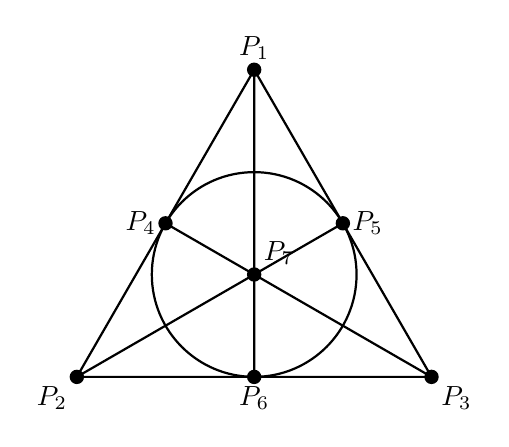
\begin{tikzpicture}[scale=1.3]
  \coordinate (A) at (90:2);   % P1
  \coordinate (B) at (210:2);  % P2
  \coordinate (C) at (330:2);  % P3
  \coordinate (AB) at ($(A)!0.5!(B)$); % P4
  \coordinate (AC) at ($(A)!0.5!(C)$); % P5
  \coordinate (BC) at ($(B)!0.5!(C)$); % P6
  \coordinate (O) at (0,0);    % P7
  \draw[thick] (A)--(B)--(C)--cycle;
  \draw[thick] (A)--(BC) (B)--(AC) (C)--(AB);
  \draw[thick] (O) circle (1);
  \foreach \p/\n/\pos in {A/P_1/above,B/P_2/below left,C/P_3/below right,AB/P_4/left,AC/P_5/right,BC/P_6/below,O/P_7/above right}{
    \fill (\p) circle (2pt); \node[\pos] at (\p) {$\n$};
  }
\end{tikzpicture}
\end{center}
これが Fano 平面の図であり，6本の線分と1つの円がちょうど7本の直線に対応する（円が直線 $x_0+x_1+x_2=0$）．

\exsol{ch08-prob-lines}
$\PP^3=\PP(k^4)$ の直線・平面は，それぞれ $k^4$ の2次元・3次元部分空間 $W$ に対応する．射影部分空間の交わり $\PP(W_1)\cap\PP(W_2)=\PP(W_1\cap W_2)$ であり，次元公式
\[
  \dim(W_1\cap W_2)=\dim W_1+\dim W_2-\dim(W_1+W_2)\ \ge\ \dim W_1+\dim W_2-4
\]
を用いる．$\PP(W_1\cap W_2)\neq\emptyset\iff\dim(W_1\cap W_2)\ge1$ である．

\textbf{2直線}：$\dim W_i=2$ なので下限は $2+2-4=0$ で，交わりが空でありうる．実際 $W_1+W_2=k^4$ のとき $W_1\cap W_2=0$ で2直線は交わらない．
例えば $L_1=\Zero(x_2,x_3)$，$L_2=\Zero(x_0,x_1)$ では $W_1=\langle e_0,e_1\rangle$，$W_2=\langle e_2,e_3\rangle$ で $W_1\cap W_2=0$．
「一般の」2つの2次元部分空間は $W_1+W_2=k^4$ を満たす（$W_1,W_2$ の基底を並べた $4\times4$ 行列式 $\neq0$ という開条件）ので，2直線は一般にはねじれの位置にある．
交わるのは $\dim(W_1+W_2)\le3$，すなわち2直線が同一平面上にあるときに限る．

\textbf{2平面}：$\dim W_i=3$ なので $\dim(W_1\cap W_2)\ge3+3-4=2$．相異なる平面なら $W_1\neq W_2$ より $W_1+W_2=k^4$ で，$\dim(W_1\cap W_2)=2$ ちょうど．よって2平面は必ず直線 $\PP(W_1\cap W_2)$ で交わる．

\textbf{直線と平面}：$\dim(W_1\cap W_2)\ge2+3-4=1$ なので交わりは空でない．直線が平面に含まれなければ $W_1+W_2=k^4$ で $\dim(W_1\cap W_2)=1$，すなわちちょうど1点で交わる．

アフィン空間 $\A^3$ では平行な平面や平行な直線と平面は交わらないが，射影空間ではそれらは無限遠平面上で交わっている．

\exsol{ch08-prob-chart}
$U_0=\{x_0\neq0\}$ の座標は $z=x_1/x_0$ であり，$\infty=[0:1]$ である．まず写像が well-defined であること：$(cx_1+dx_0,\ ax_1+bx_0)=(0,0)$ となるのは $\begin{pmatrix}d&c\\b&a\end{pmatrix}\begin{pmatrix}x_0\\x_1\end{pmatrix}=0$ のときで，行列式 $ad-bc\neq0$ より $(x_0,x_1)=(0,0)$ に限るから，像は $\PP^1$ の点である．スカラー倍とも可換である．

$[x_0:x_1]=[1:z]\in U_0$ の像は $[cz+d:az+b]$ であり，$cz+d\neq0$ ならこれは $U_0$ の点で，その $z$ 座標は
\[
  z'=\frac{az+b}{cz+d}
\]
となる．すなわち射影変換は $z$ 座標で Möbius 変換として表される．

\textbf{$\infty$ の行き先}：$[0:1]\mapsto[c:a]$．$c\neq0$ なら $z'=a/c$，$c=0$ なら（このとき $a\neq0$）$[0:a]=\infty$．
これは $\lim_{z\to\infty}(az+b)/(cz+d)=a/c$ と一致する．

\textbf{$\infty$ に行く点}：像が $[0:\ast]$ となるのは $cx_1+dx_0=0$ のとき，すなわち $[x_0:x_1]=[c:-d]$．$c\neq0$ ならこれは $U_0$ の点 $z=-d/c$（Möbius 変換の分母の零点），$c=0$ なら $[0:-d]=\infty$ 自身である．

まとめると，$c\neq0$ のとき $\infty\mapsto a/c$，$-d/c\mapsto\infty$；$c=0$ のとき $\infty\mapsto\infty$ で，変換は $U_0$ 上のアフィン変換 $z\mapsto(az+b)/d$ になる．
$\C$ 上では，Möbius 変換の「分母が0になる点」や「$z=\infty$」という例外処理が，同次座標では例外なしの線形写像として統一的に扱われているわけである．

\exsol{ch08-prob-homeo}
$U_0$ には $\PP^n$ の射影 Zariski 位相からの相対位相を入れる．すなわち $U_0$ の閉集合は $\Zero(T)\cap U_0$（$T$ は同次多項式の集合）の形の集合である．
$\varphi_0$ は全単射なので（命題\ref{prop:ch08-chart}），閉集合を閉集合に写すこと（$\varphi_0^{-1}$ の連続性）と，閉集合の逆像が閉集合であること（$\varphi_0$ の連続性）を示せばよい．

\textbf{(i) $\varphi_0(\Zero(T)\cap U_0)=\Zero(\{F_*\mid F\in T\})$．}
$U_0$ の点は $[1:a_1:\dots:a_n]$ と一意に表され，$\varphi_0$ はこれを $a=(a_1,\dots,a_n)$ に写す．同次多項式 $F$ について
\[
  [1:a]\in\Zero(F)\iff F(1,a_1,\dots,a_n)=0\iff F_*(a)=0
\]
（同次多項式の零点は代表元によらないので，代表元 $(1,a)$ で判定してよい）．よって $\varphi_0(\Zero(T)\cap U_0)=\Zero(\{F_*\mid F\in T\})$ であり，これは $\A^n$ の閉集合である．

\textbf{(ii) $\varphi_0^{-1}(\Zero(f))=\Zero(f^h)\cap U_0$．}
$f=0$ なら両辺とも $U_0$ 全体なので $f\neq0$，$\deg f=d$ とする．$[x]\in U_0$（$x_0\neq0$）について，定義から
\[
  f^h(x_0,\dots,x_n)=x_0^d\,f\Bigl(\frac{x_1}{x_0},\dots,\frac{x_n}{x_0}\Bigr)=x_0^d\,f(\varphi_0([x]))
\]
で $x_0^d\neq0$ だから，$f(\varphi_0([x]))=0\iff f^h(x)=0$．よって $\varphi_0^{-1}(\Zero(f))=\Zero(f^h)\cap U_0$．
$\A^n$ の一般の閉集合 $\Zero(S)=\bigcap_{f\in S}\Zero(f)$ については，$\varphi_0^{-1}(\Zero(S))=\Zero(\{f^h\mid f\in S\})\cap U_0$ であり，これは $U_0$ の閉集合である．

(i) より $\varphi_0$ は閉写像，(ii) より $\varphi_0$ は連続で，全単射だから同相写像である．

\exsol{ch08-prob-homprime}
\textbf{既約性．}$F=x_2\cdot x_0-x_1^2$ を $A=k[x_1,x_2]$ 係数の $x_0$ の多項式とみる．$x_0$ について1次で，係数 $x_2$ と $-x_1^2$ は $A$ で互いに素（共通の既約因子をもたない）．
$F=GH$ と分解すると，$x_0$ についての次数の和が1なので一方，例えば $G$ は $x_0$ を含まず $G\in A$．すると $G$ は $F$ の $x_0$ の係数 $x_2$ と定数項 $-x_1^2$ の両方を割り切るので，$G$ は定数である．よって $F$ は既約である．
（別証：可約なら2つの1次式の積 $F=L_1L_2$ となり，$\Zero(F)\subset\PP^2$ は2直線の和になるが，$\Zero(F)$ は $[s^2:st:t^2]$ でパラメータ付けされる既約曲線で直線を含まない．あるいは対称行列の階数が3であることからも分かる．）

\textbf{$(F)$ が同次素イデアルであること．}$S=k[x_0,x_1,x_2]$ は UFD なので，既約元 $F$ は素元であり，$(F)$ は素イデアルである．
また $(F)$ は同次多項式 $F$ で生成されるので，命題\ref{prop:ch08-homideal-char}より同次イデアルである．
さらに $(F)$ は $S_+=(x_0,x_1,x_2)$ を含まない（$x_0\notin(F)$）ので，$(F)$ は空でない射影多様体 $C=\Zero(x_0x_2-x_1^2)$（例\ref{ex:ch08-conics}の非特異2次曲線）に対応し，$\Ideal(C)=(F)$ である．

\exsol{ch08-prob-closure}
$f=y^2-x^3-x$ は1本の多項式なので $(f)^h=(f^h)$ であり（定理\ref{thm:ch08-closure-eq}の後の注意），同次化の変数を $Z$ として
\[
  \bar Y=\Zero(F),\qquad F=f^h=Y^2Z-X^3-XZ^2.
\]
\textbf{無限遠点}：$Z=0$ とおくと $F=-X^3=0$ より $X=0$．よって無限遠点は $[0:1:0]$ の\textbf{1点}のみである（$f$ の最高次成分 $-x^3$ の零点が「$y$ 軸方向」1つだけであることに対応）．

\textbf{正則性}：$[0:1:0]\in U_Y$ なので，例\ref{ex:ch08-p2chart}のチャート $(s,r)=(X/Y,Z/Y)$ を使う．$F$ を $Y^3$ で割ると
\[
  g(s,r)=F(s,1,r)=r-s^3-sr^2,
\]
無限遠点は $(s,r)=(0,0)$ である．$g\in\Ideal(\bar Y\cap U_Y)$ であり（実際 $F$ が既約なので $\Ideal(\bar Y)=(F)$，チャートでは $(g)$ が消滅イデアル），
\[
  \frac{\partial g}{\partial s}=-3s^2-r^2,\qquad \frac{\partial g}{\partial r}=1-2sr
\]
で，$(0,0)$ では $\partial g/\partial r=1\neq0$．よって Jacobian 行列の階数は $1=2-\dim\bar Y$ で，$[0:1:0]$ は $\bar Y$ の\textbf{正則点}である．
接線は $d_{(0,0)}g=r=0$，すなわち無限遠直線 $Z=0$ である．実際 $g=0$ に $r=0$ を代入すると $-s^3=0$ となり，無限遠直線とは重複度3で接している（$[0:1:0]$ は $\bar Y$ の変曲点）．
これは B\'ezout の意味で $3\cdot1=3$ 個の交点がすべて $[0:1:0]$ に集まっていることを表す（第9章）．

なお有限の部分 $Y$ も非特異である（$\mathrm{char}\,k\neq2$ で $f_y=2y$，$f_x=-(3x^2+1)$，$f=0$ の共通零点は $x^3+x$ と $3x^2+1$ の共通根だが，それは存在しない）ので，$\bar Y$ は滑らかな射影3次曲線（楕円曲線）である．

\exsol{ch08-prob-segre}
$\PP^1\times\PP^2\ni([x_0:x_1],[y_0:y_1:y_2])$ に対し $z_{ij}=x_iy_j$（$i=0,1$，$j=0,1,2$）とおくと，$\sigma$ は
\[
  \sigma([x],[y])=[z_{00}:z_{01}:z_{02}:z_{10}:z_{11}:z_{12}]\in\PP^5
\]
であり，$Z=(z_{ij})=xy^T$ は $2\times3$ 行列
$\begin{pmatrix}z_{00}&z_{01}&z_{02}\\z_{10}&z_{11}&z_{12}\end{pmatrix}$ である．例\ref{ex:ch08-segre}より像は $\rank Z\le1$ で定義され，$2\times2$ 小行列式は次の3つ：
\[
  z_{00}z_{11}-z_{01}z_{10},\qquad z_{00}z_{12}-z_{02}z_{10},\qquad z_{01}z_{12}-z_{02}z_{11}.
\]
すなわち $\sigma(\PP^1\times\PP^2)=\Zero(z_{00}z_{11}-z_{01}z_{10},\ z_{00}z_{12}-z_{02}z_{10},\ z_{01}z_{12}-z_{02}z_{11})$．

\textbf{次元}：$\Sigma=\sigma(\PP^1\times\PP^2)$ は既約（既約な $\PP^1\times\PP^2$ の像．あるいはアフィン錐が既約な $\A^2\times\A^3$ の像）である．
開集合 $\Sigma\cap\{z_{00}\neq0\}$ で $z_{00}=1$ とすると，小行列式の消滅から
\[
  z_{11}=z_{10}z_{01},\qquad z_{12}=z_{10}z_{02}
\]
が従い（第3式は前2式から自動的に成り立つ），逆にこれを満たす点は $x=(1,z_{10})$，$y=(1,z_{01},z_{02})$ の像である．
よって $\Sigma\cap U_{00}$ は $(z_{01},z_{02},z_{10})$ を自由な座標とする写像 $\A^3\to\A^2$ のグラフであり $\A^3$ と同型．既約な $\Sigma$ の空でない開集合 $\Sigma\cap U_{00}$ は稠密で，その次元は $\Sigma$ の次元に等しいから
\[
  \dim\Sigma=3=\dim\PP^1+\dim\PP^2.
\]
パラメータの勘定としては，$x\in k^2$，$y\in k^3$ の5パラメータから2つのスケール（$x\mapsto\lambda x$，$y\mapsto\mu y$）を引いて3，と見てもよい．
なお $\Sigma$ は $\PP^5$ の余次元2の多様体だが3本の2次式を必要とし，完全交差ではない（ねじれ3次曲線と同様の状況）．

\exsol{ch08-prob-bloch}
$|\psi\rangle=\alpha|0\rangle+\beta|1\rangle$，$N=\langle\psi|\psi\rangle=|\alpha|^2+|\beta|^2$ とする．Pauli 行列
$\sigma_x=\begin{pmatrix}0&1\\1&0\end{pmatrix}$，$\sigma_y=\begin{pmatrix}0&-i\\i&0\end{pmatrix}$，$\sigma_z=\begin{pmatrix}1&0\\0&-1\end{pmatrix}$ について
\begin{align*}
  \langle\psi|\sigma_x|\psi\rangle&=\bar\alpha\beta+\bar\beta\alpha=2\operatorname{Re}(\bar\alpha\beta),\\
  \langle\psi|\sigma_y|\psi\rangle&=-i\bar\alpha\beta+i\bar\beta\alpha=-i(\bar\alpha\beta-\overline{\bar\alpha\beta})=2\operatorname{Im}(\bar\alpha\beta),\\
  \langle\psi|\sigma_z|\psi\rangle&=|\alpha|^2-|\beta|^2.
\end{align*}
よって
\[
  \vec n=\frac{1}{|\alpha|^2+|\beta|^2}\bigl(2\operatorname{Re}(\bar\alpha\beta),\ 2\operatorname{Im}(\bar\alpha\beta),\ |\alpha|^2-|\beta|^2\bigr).
\]
分子・分母とも $(\alpha,\beta)$ と $(\bar\alpha,\bar\beta)$ について2次同次なので，$(\alpha,\beta)\mapsto(\lambda\alpha,\lambda\beta)$（$\lambda\in\C^*$）で $|\lambda|^2$ 倍され，比 $\vec n$ は $[\alpha:\beta]\in\C\PP^1$ だけで決まる．

\textbf{$|\vec n|=1$}：
\[
  N^2|\vec n|^2=4|\bar\alpha\beta|^2+(|\alpha|^2-|\beta|^2)^2=4|\alpha|^2|\beta|^2+|\alpha|^4-2|\alpha|^2|\beta|^2+|\beta|^4=(|\alpha|^2+|\beta|^2)^2=N^2.
\]
したがって $|\vec n|=1$ で，$\vec n$ は単位球面 $S^2$ 上にある．$(\alpha,\beta)=(\cos\frac\theta2,e^{i\varphi}\sin\frac\theta2)$ とすれば $\bar\alpha\beta=\frac12\sin\theta\,e^{i\varphi}$，$|\alpha|^2-|\beta|^2=\cos\theta$ で，例\ref{ex:ch08-bloch}の式を再現する．

\textbf{直交状態は対蹠点}：$\C^2$ で $(\alpha,\beta)$ に直交するベクトルは1次元で，$(\alpha',\beta')=(-\bar\beta,\bar\alpha)$ で張られる（$\bar\alpha\alpha'+\bar\beta\beta'=-\bar\alpha\bar\beta+\bar\beta\bar\alpha=0$）．
したがって直交する状態は $[\alpha':\beta']=[-\bar\beta:\bar\alpha]$ ただ1つであり，
\[
  \bar\alpha'\beta'=(-\beta)\bar\alpha=-\bar\alpha\beta,\qquad |\alpha'|^2-|\beta'|^2=|\beta|^2-|\alpha|^2,\qquad |\alpha'|^2+|\beta'|^2=N
\]
より $\vec n'=-\vec n$．すなわち直交する2状態は Bloch 球面上の対蹠点に写る（例：$|0\rangle\mapsto(0,0,1)$，$|1\rangle\mapsto(0,0,-1)$）．
より一般に，遷移確率は $P([\psi],[\phi])=\frac{1+\vec n_\psi\cdot\vec n_\phi}{2}$ となり，$P=0\iff\vec n_\phi=-\vec n_\psi$ である．

% ============================================================
% 第9章 射影多様体・交差・Bézoutの定理
% ============================================================
\chapter{射影多様体・交差・B\'ezoutの定理}
\label{ch:ch09}

\begin{chapterlead}
第8章で導入した射影空間 $\PP^n$ は，アフィン空間に「無限遠」を付け加えてコンパクトにした空間であった．
本章ではその中の射影多様体について，次元・次数・交差という三つの基本量を調べる．
射影空間の最大の利点は，「交わるはずのものが必ず交わる」ことである．
平面上の2直線は平行なら交わらないが，$\PP^2$ では必ずちょうど1点で交わる．
この現象を一般化したのが射影次元定理と B\'ezout の定理であり，
「次数 $d$ の曲線と次数 $e$ の曲線は，重複度を込めてちょうど $de$ 点で交わる」という美しい主張に結実する．
これは代数幾何における「数え上げ」の出発点であり，弦理論のコンパクト化に現れる交差数（湯川結合）の計算へと直接つながっている．
\end{chapterlead}

% ------------------------------------------------------------
\section{射影多様体の基本構造}
% ------------------------------------------------------------

第8章では，同次イデアル $I\subset S=k[x_0,\dots,x_n]$ の零点集合として射影代数的集合 $\Zero(I)\subset\PP^n$ を定義し，その既約なものを射影多様体と呼んだ．
本節では，アフィン多様体について第5章・第7章で調べた基本量（次元・既約性・包含関係）を射影多様体に移植する．
道具は二つある：(i) アフィン錐（affine cone）を用いて $\A^{n+1}$ の問題に帰着する方法，(ii) 標準アフィン開集合 $U_i=\{x_i\neq 0\}\cong\A^n$ に制限して局所的に調べる方法である．

\subsection{射影多様体の次元}

射影代数的集合 $X\subset\PP^n$ のアフィン錐 $C(X)\subset\A^{n+1}$（第8章で定義した．$X=\Zero(I)\neq\emptyset$ ならば $C(X)=\Zero_{\A^{n+1}}(I)$）を用いる．
$X$ の各点は $C(X)$ の原点を通る直線1本に対応するから，$C(X)$ は $X$ よりちょうど1次元「太い」はずである．

\begin{mydef}{射影代数的集合の次元}{ch09-projdim}
射影代数的集合 $X\subset\PP^n$ の\textbf{次元} $\dim X$ を，Zariski 位相空間としての次元（既約閉集合の真の増大列 $Z_0\subsetneq Z_1\subsetneq\cdots\subsetneq Z_r$ の長さ $r$ の上限）で定める．空集合の次元は $-1$ と約束する．
\end{mydef}

\begin{myprop}{次元の三通りの計算法}{ch09-dimcomp}
$X\subset\PP^n$ を空でない射影多様体とする．
\begin{enumerate}
  \item $X\cap U_i\neq\emptyset$ となる任意の $i$ について $\dim X=\dim(X\cap U_i)$．
  \item $\dim C(X)=\dim X+1$．
  \item 同次座標環 $S(X)=S/\Ideal(X)$ の Krull 次元について $\dim S(X)=\dim X+1$．
\end{enumerate}
\end{myprop}

\begin{proof}[証明の概略]
(1) $X\cap U_i$ は $X$ の空でない開集合であり，$X$ は既約だから $X\cap U_i$ は $X$ で稠密である．
既約閉集合の鎖 $Z_0\subsetneq\cdots\subsetneq Z_r$ を $X\cap U_i$ で取れば，その閉包は $X$ の鎖になり，逆に $X$ の鎖で $Z_0\cap U_i\neq\emptyset$ となるものは $U_i$ に制限しても真の包含が保たれる．
アフィン多様体の次元が「任意の極大鎖の長さが一定」であること（第7章）を使えば両者が一致する．

(2) $C(X)\setminus\{0\}$ の $\{x_i\neq0\}$ 部分は $(X\cap U_i)\times(\A^1\setminus\{0\})$ と同型である：点 $(a_0,\dots,a_n)$ に $([a],a_i)$ を対応させればよい．
よって $\dim C(X)=\dim(X\cap U_i)+1=\dim X+1$．

(3) $C(X)$ の座標環は $S(X)$ そのものであり，アフィン多様体の次元は座標環の Krull 次元に等しい（第7章）．
\end{proof}

\begin{myex}{次元の計算}{ch09-dimex}
\begin{enumerate}
  \item $\PP^n$ 自身：$C(\PP^n)=\A^{n+1}$ より $\dim\PP^n=n$．
  \item 線形部分空間 $L=\Zero(x_{r+1},\dots,x_n)\cong\PP^r$：$C(L)\cong\A^{r+1}$ なので $\dim L=r$．
  \item 平面円錐曲線 $Q=\Zero(xz-y^2)\subset\PP^2$：$C(Q)$ は $\A^3$ 内の2次錐面で次元2，ゆえに $\dim Q=1$（曲線）．実際，$z\neq0$ のチャートでは放物線 $y^2=x$ である．
  \item ねじれ3次曲線 $T=\{[s^3:s^2t:st^2:t^3]\}\subset\PP^3$：$C(T)$ は $(s,t)\mapsto(s^3,s^2t,st^2,t^3)$ の像で2次元，よって $\dim T=1$．
\end{enumerate}
\end{myex}

次元の直感は「独立なパラメータの数」である．
$\PP^n$ の点は $n+1$ 個の同次座標で書かれるが，全体のスケール倍 $\lambda\in k^\times$ の自由度を割るので $n$ 個のパラメータになる．
射影多様体も同じで，錐の次元から「スケールの1」を引いたものが次元である．

\begin{physbox}[ゲージ自由度の除去]
同次座標 $[x_0:\dots:x_n]$ はスケール変換 $x_i\mapsto\lambda x_i$ を「ゲージ冗長性」として持つ記述であり，$\PP^n=(\C^{n+1}\setminus\{0\})/\C^\times$ はゲージ固定後の物理的配位空間とみなせる．
$\dim C(X)-1=\dim X$ は「場の数 $-$ ゲージ対称性の数」という物理でおなじみの自由度の数え方そのものである．
2次元の $\mathcal N=(2,2)$ ゲージ線形シグマ模型（GLSM）では，$U(1)$ ゲージ群と D 項条件によって実際に $\PP^n$ や射影多様体が真空多様体として現れる．この点は第8章の物理的背景（\S\ref{sec:ch08-phys}）でも述べた．
\end{physbox}

\subsection{余次元}

\begin{mydef}{余次元}{ch09-codim}
$Y\subset X$ を射影多様体の閉部分多様体とするとき，$\codim_X Y=\dim X-\dim Y$ と定める．$X=\PP^n$ のときは単に $\codim Y=n-\dim Y$ と書く．
\end{mydef}

一般の位相空間では余次元を「$Y$ を含む既約閉集合の鎖の長さ」で定義するが，多様体ではこれが上の差に一致する（次元の加法性；第7章参照）．
アフィン錐を取っても余次元は変わらない：$\codim_{\A^{n+1}}C(Y)=(n+1)-(\dim Y+1)=\codim_{\PP^n}Y$．

余次元は「部分多様体を定めるのに必要な方程式の数の目安」である．実際，次の Krull の単項イデアル定理の射影版が成り立つ．

\begin{myprop}{超曲面による切断}{ch09-hypercut}
$X\subset\PP^n$ を $r$ 次元射影多様体，$F$ を定数でない同次多項式とする．
$X\not\subset\Zero(F)$ ならば，$X\cap\Zero(F)$ の各既約成分はちょうど $r-1$ 次元である．
さらに $r\ge1$ ならば $X\cap\Zero(F)\neq\emptyset$．
\end{myprop}

\begin{proof}[証明の概略]
アフィン錐で考える．$C(X)\cap\Zero(F)$ は $C(X)$ 上の1つの関数の零点集合だから，その各既約成分は $r+1-1=r$ 次元である（アフィンの単項イデアル定理，第7章）．
これらの成分は原点を含む錐であり，次元 $r\ge1$ なので原点以外の点を含む．それを $\PP^n$ に落とせば $X\cap\Zero(F)$ の $r-1$ 次元成分が得られる．
\end{proof}

アフィン空間では $\Zero(x)\cap\Zero(x-1)=\emptyset$ のように超曲面が交わらないことがあるが，射影空間では $r\ge1$ ならば決して空にならない．
これが本章を通じて繰り返される「射影空間では交差が失われない」という原理の最初の現れである．

\begin{myex}{完全交差}{ch09-ci}
$\PP^n$ 内で $c$ 個の同次多項式 $F_1,\dots,F_c$ により定まる $X=\Zero(F_1,\dots,F_c)$ は，命題\ref{prop:ch09-hypercut}を繰り返し用いると，各成分の次元が $n-c$ 以上である．
ちょうど $n-c$（すなわち余次元 $c$）で $\Ideal(X)=(F_1,\dots,F_c)$ となるとき，$X$ を\textbf{完全交差}と呼ぶ．
例えば $\PP^4$ 内の5次超曲面（余次元1）や，$\PP^5$ 内の2つの3次超曲面の交わり（余次元2）はいずれも完全交差であり，ともに Calabi--Yau 3次元多様体の代表例である（第15章）．
一方，ねじれ3次曲線 $T\subset\PP^3$ は余次元2だが，その同次イデアル $\Ideal(T)$ は2個の元では生成できず，3個の2次式
\[
  x_0x_2-x_1^2,\qquad x_1x_3-x_2^2,\qquad x_0x_3-x_1x_2
\]
で生成される（完全交差でない．例\ref{ex:ch08-twisted}も参照）．
\end{myex}

\subsection{射影多様体の既約性}

\begin{myprop}{既約性の判定}{ch09-irred}
射影代数的集合 $X\subset\PP^n$（$X\neq\emptyset$）について次は同値である．
\begin{enumerate}
  \item $X$ は既約である．
  \item 同次消滅イデアル $\Ideal(X)\subset S$ は素イデアルである．
  \item アフィン錐 $C(X)$ は既約である．
\end{enumerate}
\end{myprop}

\begin{proof}
(1)$\Leftrightarrow$(2) は第8章の命題\ref{prop:ch08-irr-prime}である．
(2)$\Leftrightarrow$(3) はアフィンの場合の対応（第4章：既約 $\Leftrightarrow$ 消滅イデアルが素）を $C(X)$ に適用したものである（$\Ideal(C(X))=\Ideal(X)$）．
\end{proof}

具体例（$\Zero(xy)$ は可約，$\Zero(x^2+y^2-z^2)$ は既約，$\Zero(x^2+y^2)$ は $\C$ 上で2直線に分解する，など）は第8章の例\ref{ex:ch08-irr-ex}を参照．

射影代数的集合も Noether 性により有限個の既約成分の和に一意的に分解する（第3章のアフィンの場合と同じ議論）．
また $X$ が既約であれば，空でない各 $X\cap U_i$ も既約であり，その射影閉包は $X$ に戻る．
逆に，アフィン多様体 $Y\subset\A^n$ の射影閉包 $\overline{Y}\subset\PP^n$ は既約で $\dim\overline{Y}=\dim Y$ である．

\subsection{射影多様体の包含関係}

アフィンの場合と同様に，同次根基イデアルと射影代数的集合の間には包含を逆転させる対応がある．
ただし射影空間特有の例外として\textbf{無関係イデアル}（irrelevant ideal）$S_+=(x_0,\dots,x_n)$ がある：$\Zero(S_+)$ は $\A^{n+1}$ では原点だが，原点は $\PP^n$ の点ではないので $\PP^n$ では空集合となる．
第8章の射影零点定理（定理\ref{thm:ch08-projnull}）により，$\Zero(I)=\emptyset\iff\sqrt I\supset S_+$ であり，$\Zero(I)\neq\emptyset$ ならば $\Ideal(\Zero(I))=\sqrt I$ である．
したがって $X\mapsto\Ideal(X)$ は，空でない射影代数的集合と $S_+$ を含まない同次根基イデアルの間の包含逆転の全単射を与え，射影多様体は $S_+$ を含まない同次素イデアルに対応する．

包含関係については次の基本的な事実が重要である．

\begin{myprop}{次元と包含}{ch09-inclusion}
$X\subset Y$ を射影多様体とする．$\dim X=\dim Y$ ならば $X=Y$．とくに $X\subsetneq Y$ なら $\dim X<\dim Y$．
\end{myprop}

\begin{proof}
$X\subsetneq Y$ なら，$X$ で終わる既約閉集合の極大鎖に $Y$ を付け加えることで長さが1増えるので $\dim Y\ge\dim X+1$．
\end{proof}

例えば，次数2の既約曲線 $Q\subset\PP^2$ を含む既約閉集合は $Q$ 自身か $\PP^2$ 全体しかない．
この単純な事実は，後で「2つの曲線が共通成分を持たなければ交わりは有限集合」という形で B\'ezout の定理の仮定に現れる．

\exprob{prob:ch09-1}
$\PP^3$ 内の2つの2次曲面 $Q_1=\Zero(x_0x_3-x_1x_2)$ と $Q_2=\Zero(x_0x_2-x_1^2)$ の共通部分 $Q_1\cap Q_2$ を既約成分に分解し，各成分の次元を求めよ．
（ヒント：ねじれ3次曲線と1本の直線に分かれる．）

\exprob{prob:ch09-2}
$X\subset\PP^n$ が空でない射影多様体で $\dim X\ge1$ のとき，任意の超平面 $H$ について $X\cap H\neq\emptyset$ であることを示せ．
また，アフィン空間ではこの主張が成り立たない例を挙げよ．

% ------------------------------------------------------------
\section{超曲面}
% ------------------------------------------------------------

\subsection{超曲面の定義}

\begin{mydef}{射影超曲面}{ch09-hypersurface}
定数でない同次多項式 $F\in k[x_0,\dots,x_n]_d$ の零点集合 $\Zero(F)\subset\PP^n$ を\textbf{（射影）超曲面}という．
$F$ を既約因子の積 $F=F_1^{m_1}\cdots F_s^{m_s}$ に分解したとき，$\Zero(F)=\Zero(F_1)\cup\dots\cup\Zero(F_s)$ が既約分解である．
$F$ が既約のとき $\Zero(F)$ は既約超曲面で，$\Ideal(\Zero(F))=(F)$ となる．
\end{mydef}

$n=2$ なら平面曲線，$n=3$ なら曲面である．命題\ref{prop:ch09-hypercut}（$X=\PP^n$ の場合）から，超曲面の各既約成分はちょうど $n-1$ 次元である．
逆に，$\PP^n$ の余次元1の既約部分多様体は必ず既約超曲面である：$S$ は UFD なので，高さ1の同次素イデアルは単項 $(F)$ で生成されるからである．

重複度 $m_i\ge2$ の因子は零点集合からは見えない．すなわち零点集合だけを見ると「方程式としての情報」が失われている．
例えば $\Zero(x^2)$ と $\Zero(x)$ は集合としては同じ直線だが，前者は「2重の直線」と考えるのが自然である．
こうした重複構造を正しく扱うのがスキーム論であり，第12章で詳しく扱う．
本章ではこれを\textbf{因子} $\sum m_i\,\Zero(F_i)$ として形式的に記録する（9.5節）．

\subsection{次数}

\begin{mydef}{超曲面の次数}{ch09-degree-hyp}
既約超曲面 $\Zero(F)$ の\textbf{次数}を $\deg F$ と定める．
より一般に，$F=\prod F_i^{m_i}$ に対して因子 $\sum m_i\Zero(F_i)$ の次数を $\deg F=\sum m_i\deg F_i$ とする．
\end{mydef}

次数の幾何学的意味は「一般の直線との交点の数」である．
直線 $L$ を $t\mapsto[a+tb]$（$a,b\in k^{n+1}$）とパラメータ表示すると，$F(sa+tb)$ は $(s,t)$ について $d$ 次の2変数同次式である．
これが恒等的に $0$ でなければ（$L\not\subset\Zero(F)$），代数閉体上で $d$ 個の1次式の積に分解する：
\[
  F(sa+tb)=c\prod_{j=1}^{d}(\beta_j s-\alpha_j t).
\]
各根 $[\alpha_j:\beta_j]\in\PP^1$ が交点 $L\cap\Zero(F)$ に対応し，重根は接触を表す．
したがって\emph{重複度を込めれば}直線と次数 $d$ の超曲面はちょうど $d$ 点で交わる．これは B\'ezout の定理の最も簡単な場合である．

\paragraph{Hilbert 多項式による次数．}
一般の射影多様体（超曲面でないもの）の次数は，Hilbert 多項式で定義するのが標準的である．
$X\subset\PP^n$ に対し，同次座標環 $S(X)=S/\Ideal(X)$ の $m$ 次部分の次元
\[
  h_X(m)=\dim_k S(X)_m
\]
を Hilbert 関数という．これは「$X$ 上の $m$ 次の同次多項式関数の個数」である．

\begin{mythm}{Hilbert 多項式}{ch09-hilbpoly}
$X\subset\PP^n$ を $r$ 次元射影代数的集合とする．十分大きな $m$ に対して $h_X(m)$ はある多項式 $P_X(m)\in\Q[m]$ に一致し，その次数は $r$ で，
\[
  P_X(m)=\frac{d}{r!}m^r+(\text{低次の項})
\]
の形となる．ここで $d$ は正の整数であり，これを $X$ の\textbf{次数} $\deg X$ と定める．
\end{mythm}

証明は次数付き加群の短完全列と次元に関する帰納法による（ここでは省略する）．
大事なのは定義の整合性で，超曲面ではこれが上の次数と一致する．

\begin{myex}{超曲面の Hilbert 多項式}{ch09-hilbhyp}
$X=\Zero(F)\subset\PP^n$，$\deg F=d$ とする．$S(X)=S/(F)$ であり，$F$ 倍写像による完全列
\[
  0\to S_{m-d}\xrightarrow{\ \cdot F\ }S_m\to S(X)_m\to0
\]
から，$\dim S_m=\binom{m+n}{n}$ を用いて
\[
  h_X(m)=\binom{m+n}{n}-\binom{m-d+n}{n}=\frac{d}{(n-1)!}m^{n-1}+\cdots.
\]
よって $\deg X=d$ であり，定義\ref{def:ch09-degree-hyp}と一致する．
とくに平面曲線（$n=2$）では
\[
  P_X(m)=dm-\frac{d(d-3)}{2}=dm+1-\frac{(d-1)(d-2)}{2}
\]
となり，定数項 $1-g$ から滑らかな平面曲線の種数 $g=\frac{(d-1)(d-2)}{2}$ が読み取れる（第13章の Riemann 面の種数と一致する）．
\end{myex}

\begin{myex}{非超曲面の次数}{ch09-hilbother}
\begin{enumerate}
  \item 線形部分空間 $\PP^r\subset\PP^n$：$S(X)=k[x_0,\dots,x_r]$ より $h(m)=\binom{m+r}{r}=\frac{m^r}{r!}+\cdots$，次数1．
  \item ねじれ3次曲線 $T$：$S(T)_m$ は $s,t$ の $3m$ 次単項式全体と同一視でき，$h(m)=3m+1$．次数3．実際，一般の平面 $a_0x_0+\dots+a_3x_3=0$ との交点は $a_0s^3+a_1s^2t+a_2st^2+a_3t^3=0$ の3根に対応する．
\end{enumerate}
\end{myex}

次数の幾何学的意味は，一般に「$r$ 次元多様体 $X\subset\PP^n$ と一般の余次元 $r$ の線形部分空間との交点の数」である．
これが Bézout の定理の高次元版（9.4.5小節）へとつながる．

\subsection{超曲面の例}

\begin{myex}{低次の超曲面}{ch09-hypex}
\begin{enumerate}
  \item \textbf{超平面}（$d=1$）：$a_0x_0+\dots+a_nx_n=0$．$\PP^{n-1}$ と同型．超平面全体は双対射影空間 $(\PP^n)^\vee$ をなす．
  \item \textbf{2次超曲面}（$d=2$）：$F=x^{\mathsf T}Ax$（$A$ は対称行列，$\mathrm{char}\,k\neq2$）．$k=\C$ では $\rank A$ のみで分類され，$\rank A=n+1$ のとき滑らか．
  $\PP^3$ 内の滑らかな2次曲面 $\Zero(x_0x_3-x_1x_2)$ は Segre 埋め込み
  \[
    \PP^1\times\PP^1\to\PP^3,\quad([s_0:s_1],[t_0:t_1])\mapsto[s_0t_0:s_0t_1:s_1t_0:s_1t_1]
  \]
  の像であり，2方向の直線族（ルーリング）を持つ．
  \item \textbf{3次曲面}（$d=3$）：滑らかな3次曲面はちょうど27本の直線を含む（Cayley--Salmon の定理）．Fermat 3次曲面 $x_0^3+x_1^3+x_2^3+x_3^3=0$ はその典型例である．
  \item \textbf{4次曲面}（$d=4$, $n=3$）：滑らかな4次曲面は K3 曲面であり，2次元の Calabi--Yau 多様体である．
  \item \textbf{5次3次元超曲面}（$d=5$, $n=4$）：$x_0^5+\dots+x_4^5=0$ などの滑らかな5次超曲面は Calabi--Yau 3次元多様体であり，弦理論のコンパクト化で最も有名な例である（第15章）．
\end{enumerate}
\end{myex}

最後の2例に共通するのは $d=n+1$ という関係である．これは「標準束が自明」であるための条件であり，第15章で詳しく扱う．

\begin{figure}[htbp]
\centering
\begin{tikzpicture}[scale=0.9]
  % conic
  \draw[thick,blue] (-2.2,0) ellipse (1.4 and 0.9);
  \node[blue] at (-2.2,-1.3) {$d=2$: 円錐曲線};
  % cubic y^2 = x^3 - x
  \begin{scope}[xshift=3.2cm]
    \draw[thick,red,domain=-0.999:0,samples=80] plot ({\x},{sqrt(\x*\x*\x-\x)});
    \draw[thick,red,domain=-0.999:0,samples=80] plot ({\x},{-sqrt(\x*\x*\x-\x)});
    \draw[thick,red,domain=1.001:1.75,samples=60] plot ({\x},{sqrt(\x*\x*\x-\x)});
    \draw[thick,red,domain=1.001:1.75,samples=60] plot ({\x},{-sqrt(\x*\x*\x-\x)});
    \node[red] at (0.4,-2.1) {$d=3$: $y^2=x^3-x$};
  \end{scope}
  \draw[->,gray] (-4.2,0)--(5.4,0);
\end{tikzpicture}
\caption{実平面に描いた超曲面（平面曲線）の例．3次曲線 $y^2=x^3-x$ の実部分は2つの連結成分を持つが，$\C$ 上では1つのトーラス（種数1）である．}
\label{fig:ch09-hypex}
\end{figure}

\subsection{高次元超曲面}

$\PP^n$ 内の $d$ 次超曲面全体は，係数を同次座標と見ることで射影空間
\[
  \PP\bigl(k[x_0,\dots,x_n]_d\bigr)\cong\PP^{N},\qquad N=\binom{n+d}{d}-1
\]
によってパラメータ付けられる（スカラー倍は同じ超曲面を与えるので射影化する）．
例えば平面3次曲線は $N=\binom{5}{2}-1=9$ 次元，$\PP^4$ 内の5次超曲面は $N=\binom{9}{4}-1=125$ 次元の族をなす．

\paragraph{滑らかさの判定．}
$X=\Zero(F)$ の点 $p$ が特異点であるのは，すべての偏微分 $\partial F/\partial x_i$ が $p$ で消えるときである．
実際，チャート $U_0$ で $f=F(1,x_1,\dots,x_n)$ に Jacobian 判定法（第7章）を適用し，Euler の恒等式
\[
  \sum_{i=0}^n x_i\frac{\partial F}{\partial x_i}=d\cdot F
\]
を使えば，$\mathrm{char}\,k\nmid d$ のとき「$F(p)=0$ かつ $\partial_iF(p)=0\ (i\ge1)$」と「$\partial_iF(p)=0\ (i\ge0)$」が同値であることがわかる．
すなわち
\[
  \Sing\Zero(F)=\Zero\Bigl(\frac{\partial F}{\partial x_0},\dots,\frac{\partial F}{\partial x_n}\Bigr).
\]

\begin{myex}{Fermat 超曲面とその変形}{ch09-fermat}
$F=x_0^d+\dots+x_n^d$ では $\partial_iF=dx_i^{d-1}$ が同時に消えるのは $x=0$ のみなので，$\mathrm{char}\,k\nmid d$ なら $\Zero(F)$ は滑らかである．
一方，Dwork 族
\[
  F_\psi=x_0^5+x_1^5+x_2^5+x_3^5+x_4^5-5\psi\,x_0x_1x_2x_3x_4
\]
では，$\psi^5=1$ のとき特異点が現れる（例えば $\psi=1$ では $[1:1:1:1:1]$ が特異点）．
実際 $\partial_iF_\psi=5(x_i^4-\psi\prod_{j\neq i}x_j)$ であり，$x_i=1$ をすべて代入すると $5(1-\psi)$ となる．
この「特異点を持つパラメータ値」は，ミラー対称性において円錐点（conifold 点）と呼ばれる重要な点である．
\end{myex}

「一般の」$d$ 次超曲面は滑らかである：特異な超曲面全体は $\PP^N$ の中の超曲面（判別式超曲面）をなし，その補集合は空でない開集合だからである．

\subsection{超曲面と代数方程式}

アフィンの方程式 $f(x_1,\dots,x_n)=0$（$\deg f=d$）は，\textbf{同次化}
\[
  F(x_0,x_1,\dots,x_n)=x_0^{d}\,f\!\left(\frac{x_1}{x_0},\dots,\frac{x_n}{x_0}\right)
\]
によって射影超曲面 $\Zero(F)$ を定める．$\Zero(F)\cap U_0=\Zero(f)$ であり，$\Zero(F)$ は $\Zero(f)$ の射影閉包である．
新しく付け加わった点 $\Zero(F)\cap\{x_0=0\}$ は「無限遠点」であり，$f$ の最高次斉次部分 $f_d$ の零点 $\Zero(f_d)\subset\PP^{n-1}$ に一致する．

\begin{myex}{2次曲線の無限遠点}{ch09-conicinfty}
平面 2次曲線（$x,y$ アフィン座標，$z$ を同次化の変数とする）について：
\begin{center}
\renewcommand{\arraystretch}{1.3}
\begin{tabular}{llll}
\hline
アフィン方程式 & 同次化 & 無限遠点 $z=0$ & 個数 \\
\hline
楕円 $x^2+2y^2=1$ & $x^2+2y^2-z^2$ & $x^2+2y^2=0$ & 2（虚） \\
双曲線 $xy=1$ & $xy-z^2$ & $[1:0:0],[0:1:0]$ & 2（実） \\
放物線 $y=x^2$ & $yz-x^2$ & $[0:1:0]$ & 1（重複度2） \\
\hline
\end{tabular}
\end{center}
射影平面では3者はすべて同じ非退化円錐曲線であり，違いは「無限遠直線 $z=0$ とどう交わるか」だけである．
放物線は無限遠直線に\emph{接している}．いずれも重複度込みで交点数は $2=\deg$ である．
\end{myex}

\begin{physbox}[境界条件としての無限遠点]
物理では解の「無限遠での振る舞い」が問題になることが多い．
代数方程式の解の個数を数えるとき，アフィン空間だけで数えると解が無限遠に「逃げて」個数が変化する．
例えば $xy=\varepsilon$ と $x=0$ は $\varepsilon\neq0$ で交わらないが，射影平面で見ると無限遠点 $[0:1:0]$ で交わっている．
パラメータを動かしても保存される量（交点数）を得るには，コンパクト化（射影化）が不可欠である．
これは，場の理論の真空の数（Witten 指数など）が「無限遠に逃げる真空」がないときにのみ不変量となる事情と並行している．
\end{physbox}

\exprob{prob:ch09-3}
$\PP^2$ 内の3次曲線 $C:\ y^2z=x^3+axz^2+bz^3$ が滑らかであるための必要十分条件が $4a^3+27b^2\neq0$ であることを，$\Sing C=\Zero(\partial_xF,\partial_yF,\partial_zF)$ を用いて示せ（$\mathrm{char}\,k\neq2,3$）．
また $C$ の無限遠点を求めよ．

% ------------------------------------------------------------
\section{多様体の交差}
% ------------------------------------------------------------

\subsection{交差の定義}

\begin{mydef}{交差}{ch09-intersection}
射影代数的集合 $X=\Zero(I)$, $Y=\Zero(J)\subset\PP^n$ の\textbf{交差}（集合論的交差）は
\[
  X\cap Y=\Zero(I)\cap\Zero(J)=\Zero(I+J)
\]
である．とくに $X\cap Y$ は再び射影代数的集合である．
\end{mydef}

集合としての交差は簡単だが，イデアル $I+J$ は一般に根基イデアルではなく，そこに「接し方」の情報が含まれている．
例えば $X=\Zero(y)$（$x$ 軸），$Y=\Zero(y-x^2)$（放物線）なら $I+J=(y,x^2)$ であり，交差は原点1点だが，$k[x,y]/(y,x^2)\cong k[x]/(x^2)$ は2次元である．
この「2」が交わりの重複度であり，9.3.5小節で定式化する．

\begin{figure}[htbp]
\centering
\begin{tikzpicture}[scale=1.0]
  \begin{scope}
    \draw[->,gray] (-1.8,0)--(1.8,0);
    \draw[thick,blue,domain=-1.3:1.3,samples=50] plot (\x,{\x*\x});
    \draw[thick,red] (-1.8,0.6)--(1.8,0.6);
    \fill (-0.775,0.6) circle (1.6pt) (0.775,0.6) circle (1.6pt);
    \node at (0,-0.6) {$y=c\ (c>0)$: 2点};
  \end{scope}
  \begin{scope}[xshift=4.5cm]
    \draw[->,gray] (-1.8,0)--(1.8,0);
    \draw[thick,blue,domain=-1.3:1.3,samples=50] plot (\x,{\x*\x});
    \draw[thick,red] (-1.8,0)--(1.8,0);
    \fill (0,0) circle (2pt);
    \node at (0,-0.6) {$y=0$: 1点（重複度2）};
  \end{scope}
  \begin{scope}[xshift=9cm]
    \draw[->,gray] (-1.8,0)--(1.8,0);
    \draw[thick,blue,domain=-1.3:1.3,samples=50] plot (\x,{\x*\x});
    \draw[thick,red] (-1.8,-0.5)--(1.8,-0.5);
    \node at (0,-0.9) {$y=c\ (c<0)$: 虚の2点};
  \end{scope}
\end{tikzpicture}
\caption{放物線 $y=x^2$ と直線 $y=c$ の交差．$c\to0$ で2交点が合流して接点となり，$c<0$ では複素共役な2点 $x=\pm\sqrt{c}$ になる．$\C$ 上では重複度込みで常に2点である．}
\label{fig:ch09-tangent}
\end{figure}

\subsection{交差の次元}

アフィン空間での基本定理（第7章で扱った単項イデアル定理の帰結）を思い出そう：
$X,Y\subset\A^n$ を多様体とすると，$X\cap Y$ の任意の既約成分 $Z$ について $\dim Z\ge\dim X+\dim Y-n$．
これは $X\cap Y\cong(X\times Y)\cap\Delta$（$\Delta\subset\A^n\times\A^n$ は対角線）と見て，$\Delta$ が $n$ 個の方程式 $x_i-y_i=0$ で切り出されることから従う．
射影空間ではさらに「空でない」ことまで言える．

\begin{mythm}{射影次元定理}{ch09-projdimthm}
$X,Y\subset\PP^n$ を射影多様体とし，$\dim X=r$, $\dim Y=s$ とする．
このとき $X\cap Y$ の任意の既約成分は次元 $\ge r+s-n$ を持つ．
さらに $r+s\ge n$ ならば $X\cap Y\neq\emptyset$ である．
\end{mythm}

\begin{proof}
アフィン錐 $C(X),C(Y)\subset\A^{n+1}$ はそれぞれ次元 $r+1$, $s+1$ であり，ともに原点を含む．
アフィンの次元定理より，$C(X)\cap C(Y)$ の原点を含む既約成分 $W$ は
\[
  \dim W\ge(r+1)+(s+1)-(n+1)=r+s-n+1
\]
を満たす．$r+s\ge n$ なら $\dim W\ge1$ なので，$W$ は原点以外の点を含み，それが $X\cap Y$ の点を与える．
成分の次元の評価は，$C(X\cap Y)=C(X)\cap C(Y)$ の各成分が錐であり，その次元が対応する $X\cap Y$ の成分の次元 $+1$ であることから従う．
\end{proof}

\begin{myex}{射影次元定理の例}{ch09-projdimex}
\begin{enumerate}
  \item $\PP^2$ の2曲線（$r=s=1$, $n=2$）：$r+s-n=0$ なので必ず交わる．平行線も無限遠点で交わる．
  \item $\PP^3$ の2平面（$r=s=2$）：少なくとも直線で交わる．
  \item $\PP^3$ の曲線と曲面（$r=1,s=2$）：必ず交わる．
  \item $\PP^3$ の2直線（$r=s=1$）：$r+s-n=-1<0$ なので交わらないこともある（ねじれの位置）．
\end{enumerate}
\end{myex}

\begin{note}
アフィン空間で $r+s\ge n$ でも交わらない例（平行な2直線）があるのは，交わりが無限遠に逃げているからである．
射影次元定理はその逃げ場を塞いだことの帰結である．
\end{note}

\subsection{一般位置}

「一般の」2つの部分多様体は，期待される次元でもっとも素直に交わる．これを2段階で定式化する．

\begin{mydef}{固有交差・横断交差}{ch09-generalpos}
$X,Y\subset\PP^n$ を射影多様体とする．
\begin{enumerate}
  \item $X\cap Y$ のすべての既約成分が次元 $\dim X+\dim Y-n$ を持つとき（$<0$ なら $X\cap Y=\emptyset$ のとき），$X$ と $Y$ は\textbf{固有に交わる}（proper intersection）という．
  \item 点 $p\in X\cap Y$ で $X,Y$ がともに滑らかで，接空間について
  \[
    T_pX+T_pY=T_p\PP^n
  \]
  が成り立つとき，$X$ と $Y$ は $p$ で\textbf{横断的に交わる}（transversal）という．
  すべての交点で横断的なとき，$X,Y$ は\textbf{一般位置にある}という．
\end{enumerate}
\end{mydef}

横断的な点では $\dim T_p(X\cap Y)=\dim T_pX+\dim T_pY-n$ となり，交わりはその点の近傍で滑らかで期待次元を持つ．
2曲線 $C,D\subset\PP^2$ の場合，横断的であるとは「交点で両者が滑らかで接線が異なる」ことである．

\begin{figure}[htbp]
\centering
\begin{tikzpicture}[scale=1.0]
  \begin{scope}
    \draw[thick,blue] (-1.3,-0.9)--(1.3,0.9);
    \draw[thick,red] (-1.3,0.9)--(1.3,-0.9);
    \fill (0,0) circle (2pt);
    \node at (0,-1.4) {横断的（$I_p=1$）};
  \end{scope}
  \begin{scope}[xshift=4cm]
    \draw[thick,blue,domain=-1.2:1.2,samples=50] plot (\x,{0.7*\x*\x});
    \draw[thick,red] (-1.4,0)--(1.4,0);
    \fill (0,0) circle (2pt);
    \node at (0,-1.4) {接する（$I_p=2$）};
  \end{scope}
  \begin{scope}[xshift=8cm]
    \draw[thick,blue,domain=-1:1,samples=60] plot ({\x*\x},{\x*\x*\x});
    \draw[thick,red] (-0.6,0)--(1.4,0);
    \fill (0,0) circle (2pt);
    \node at (0.4,-1.4) {尖点を通る（$I_p=3$）};
  \end{scope}
\end{tikzpicture}
\caption{2曲線の交わり方と交点の重複度．左：異なる接線で交わる．中：$y=x^2$ と $y=0$．右：尖点 $y^2=x^3$ と $y=0$（$k[x,y]/(y,\,y^2-x^3)\cong k[x]/(x^3)$ より重複度3）．}
\label{fig:ch09-transversal}
\end{figure}

「一般の」という言葉は，パラメータ空間の空でない Zariski 開集合上で成り立つ，という意味で用いる．
次の定理は射影空間における「一般位置への移動」を保証する．

\begin{mythm}{Kleiman 型の一般位置定理（$\mathrm{char}\,k=0$）}{ch09-kleiman}
$X,Y\subset\PP^n$ を滑らかな射影多様体とする．射影変換群 $\PGL_{n+1}(k)$ の空でない Zariski 開集合に属する $g$ について，$X$ と $gY$ は一般位置にあり，とくに固有に交わる．
\end{mythm}

これは $\PGL_{n+1}$ が $\PP^n$ に推移的に作用することから，Sard の定理の代数版（一般ファイバーの滑らかさ）を用いて示される．
物理的には「一般のパラメータでは縮退が解ける」という直感の厳密な表現である．

\subsection{交差の有限性}

\begin{myprop}{0次元の交差は有限}{ch09-finite}
$X,Y\subset\PP^n$ が固有に交わり $\dim X+\dim Y=n$ ならば，$X\cap Y$ は空でない有限集合である．
\end{myprop}

\begin{proof}
射影次元定理より空でない．固有交差の仮定よりすべての既約成分は0次元すなわち1点であり，Noether 性より既約成分は有限個である．
\end{proof}

とくに $\PP^2$ 内の2曲線 $C=\Zero(F)$, $D=\Zero(G)$ について：

\begin{mycor}{平面曲線の交差}{ch09-planefinite}
$F,G$ が共通因子を持たなければ $C\cap D$ は空でない有限集合である．
\end{mycor}

\begin{proof}
$C\cap D$ が1次元の成分 $E$ を含めば，命題\ref{prop:ch09-inclusion}より $E$ は $C$ の既約成分かつ $D$ の既約成分であり，$F,G$ はともに $E$ の定義多項式で割り切れる．
\end{proof}

アフィンの場合，有限性は「座標環 $k[x,y]/(f,g)$ が有限次元」と言い換えられる．
実際，$k[x,y]/(f,g)$ は中国剰余定理によって各交点での局所環の直積に分解する：
\begin{equation}\label{eq:ch09-crt}
  k[x,y]/(f,g)\;\cong\;\prod_{p\in\Zero(f,g)}\OO_{\A^2,p}/(f,g).
\end{equation}
左辺の次元は交点の総数を重複度込みで数えたものであり，右辺の各因子の次元がその点での重複度である．

\subsection{交差の重複度}

第6章で定義した局所環 $\OO_{X,p}$（$p$ の近傍で定義された有理関数のなす環）を使って，交点の重複度を定義する．

\begin{mydef}{交点の重複度（平面曲線）}{ch09-intmult}
$C=\Zero(F)$, $D=\Zero(G)\subset\PP^2$ を共通成分を持たない曲線，$p\in\PP^2$ とする．
$p$ を含むアフィンチャート（例えば $U_2=\{z\neq0\}$）で $f=F(x,y,1)$, $g=G(x,y,1)$ とおき，
\[
  I_p(C,D)\;=\;\dim_k\,\OO_{\PP^2,p}/(f,g)
\]
を $p$ における $C$ と $D$ の\textbf{交点の重複度}（局所交差数）という．
\end{mydef}

$\OO_{\PP^2,p}/(f,g)$ は Artin 局所環であり，その $k$ 上の次元は環の長さに等しい．
定義はチャートの取り方によらない：別のチャートでは $f,g$ が単元倍（$z^{-\deg F}$ 倍など）されるだけだからである．

\begin{myex}{直線と円錐曲線}{ch09-lineconic}
$C=\Zero(yz-x^2)$（放物線），$D_c=\Zero(y-cz)$ とする．$U_2$ で $f=y-x^2$, $g=y-c$．
\begin{itemize}
  \item $c\neq0$：$(f,g)=(y-c,\,x^2-c)=(y-c,(x-\sqrt c)(x+\sqrt c))$．2点 $(\pm\sqrt c,c)$ でそれぞれ $\OO_p/(f,g)\cong k$ なので $I_p=1$．
  \item $c=0$：原点で $\OO_{p}/(y-x^2,\,y)\cong k[x]_{(x)}/(x^2)$ で，基底 $\{1,x\}$ より $I_p=2$．
\end{itemize}
いずれも交点の重複度の和は $2=1\cdot2$ である．
一方，「縦の直線」$D'=\Zero(x)$ は $U_2$ で原点 $(0,0)$ に $I=1$ で交わり，さらに無限遠点 $[0:1:0]$ でも交わる．$U_1=\{y\neq0\}$ で $f=z-x^2$, $g=x$ とすると $\OO_p/(z-x^2,x)\cong k$ で $I=1$．やはり合計2である．
\end{myex}

\begin{note}
一般次元の部分多様体 $X,Y\subset\PP^n$ が孤立点 $p$ で固有に交わるとき，$\dim_k\OO_{\PP^n,p}/(\Ideal(X)+\Ideal(Y))$ が正しい重複度を与えるのは，$X,Y$ が $p$ で Cohen--Macaulay（例えば滑らか）な場合であり，一般にはこれは正しくない．
一般には Serre の Tor 公式
$I_p(X,Y)=\sum_{i\ge0}(-1)^i\,\mathrm{length}\,\mathrm{Tor}_i^{\OO_{\PP^n,p}}(\OO_{X,p},\OO_{Y,p})$
が正しい定義である．平面曲線ではつねに Cohen--Macaulay なので上の定義で十分である．
\end{note}

\exprob{prob:ch09-4}
$\A^2$ 上で次の交点の重複度 $I_{(0,0)}$ を計算せよ．
(a) $y-x^3$ と $y$，\quad
(b) $y^2-x^3$ と $y-x$，\quad
(c) $y^2-x^2(x+1)$（結節点）と $y$，\quad
(d) $y^2-x^3$ と $x^2-y^3$．

% ------------------------------------------------------------
\section{B\'ezoutの定理}
% ------------------------------------------------------------

\subsection{B\'ezoutの定理の主張}

\begin{mythm}{B\'ezout の定理}{ch09-bezout}
$k$ を代数閉体とし，$C,D\subset\PP^2$ をそれぞれ次数 $d,e$ の共通成分を持たない平面曲線とする．このとき
\[
  \sum_{p\in C\cap D}I_p(C,D)=d\cdot e.
\]
とくに $C$ と $D$ は少なくとも1点，高々 $de$ 点で交わる．
\end{mythm}

この定理の3つの仮定はいずれも本質的である．
\begin{itemize}
  \item \textbf{代数閉体}：$\R$ 上では $x^2+y^2=z^2$ と $x=2z$ は（実の）交点を持たない．
  \item \textbf{射影空間}：$\A^2$ では平行線のように交点が無限遠に逃げる．
  \item \textbf{重複度}：接するときに交点が合流する（図\ref{fig:ch09-tangent}）．
\end{itemize}
3つの「補正」をすべて入れたときにはじめて，交点の数はパラメータによらない不変量 $de$ になる．

\subsection{射影平面における曲線の交点}

証明に入る前に，交点が射影平面全体にどう分布するかを見ておく．アフィンチャート $U_2=\{z\neq0\}$ での交点（「有限の交点」）と，無限遠直線 $z=0$ 上の交点がある．
無限遠の交点は，$F,G$ の最高次斉次部分 $f_d,g_e$ の共通零点に対応する．

\begin{myex}{平行線}{ch09-parallel}
$y=x$ と $y=x+1$ の同次化 $y-x=0$，$y-x-z=0$ は $z=0$, $y=x$ すなわち $[1:1:0]$ で交わる．
平行線は「同じ方向の無限遠点」を共有する．方向 $(1,1)$ が無限遠点 $[1:1:0]$ である．
\end{myex}

\begin{myex}{有限交点の消失}{ch09-escape}
$f=xy-1$（双曲線）と $g=x$ はアフィン平面では交わらない．
同次化 $F=xy-z^2$, $G=x$ では $x=0\Rightarrow z=0$ となり，交点は $[0:1:0]$ のみ．
$U_1=\{y\neq0\}$ で $x-z^2$ と $x$ を考えると $\OO_p/(x-z^2,x)\cong k[z]_{(z)}/(z^2)$ で $I_p=2$．
双曲線は漸近線 $x=0$ に無限遠で接しており，合計 $2=2\cdot1$ となる．
\end{myex}

\subsection{交点の重複度}

B\'ezout の定理の証明と計算で用いる，局所交差数 $I_p$ の基本性質をまとめる（Fulton の公理系）．
$F,G,H$ は同次多項式で，$p$ を含むアフィンチャートで考える．

\begin{myprop}{交点の重複度の性質}{ch09-multprop}
\begin{enumerate}
  \item $F,G$ が $p$ を通る共通成分を持てば $I_p=\infty$，持たなければ $I_p(F,G)$ は非負整数．
  \item $I_p(F,G)=0$ $\iff$ $p\notin\Zero(F)\cap\Zero(G)$．
  \item 射影変換 $T$ について $I_{T(p)}(F\circ T^{-1},G\circ T^{-1})=I_p(F,G)$．
  \item（対称性）$I_p(F,G)=I_p(G,F)$．
  \item（下界）$I_p(F,G)\ge m_p(F)\,m_p(G)$．等号 $\iff$ $F,G$ が $p$ で共通の接線を持たない．
  ここで $m_p(F)$ は $p$ における $F$ の重複度（$p$ を原点としたときの最低次項の次数）．
  \item（加法性）$I_p(F,GH)=I_p(F,G)+I_p(F,H)$．
  \item（変形不変性）任意の多項式 $A$ について $I_p(F,G+AF)=I_p(F,G)$．
\end{enumerate}
\end{myprop}

(4),(7) は定義から明らか（イデアル $(f,g)=(f,g+af)$）．(6) は完全列
\[
  0\to\OO_p/(f,h)\xrightarrow{\ \cdot g\ }\OO_p/(f,gh)\to\OO_p/(f,g)\to0
\]
（$f,g$ が共通成分を持たないことから左の写像は単射）から従う．
特に $m_p(F)=1$ かつ $m_p(G)=1$（両方滑らか）のとき，$I_p=1$ $\iff$ 接線が異なる $\iff$ 横断的，である．

これらの性質を使うと，$I_p$ は Euclid の互除法のように計算できる．

\begin{myex}{2つの尖点曲線の交わり}{ch09-twocusps}
$f=y^2-x^3$, $g=x^2-y^3$ の原点での交点の重複度を求める．
$m_0(f)=m_0(g)=2$ であり，接錐はそれぞれ $y^2$, $x^2$ で共通接線を持たないから，(5) より $I_0(f,g)=2\cdot2=4$．
この2曲線は $\PP^2$ で $3\cdot3=9$ 点で交わるから，原点以外に重複度込みで5個の交点がある．
実際，$y^2=x^3$, $x^2=y^3$ から $x^4=y^6=x^9$ で，$x\neq0$ なら $x^5=1$ となり，$x=\zeta$（$\zeta^5=1$）に対し $y=y^3/y^2=\zeta^2/\zeta^3=\zeta^4$ と一意に決まる．これで5点．無限遠では $F=y^2z-x^3$, $G=x^2z-y^3$ が $z=0$ で $x=y=0$ となり交わらない．合計 $4+5=9$．
\end{myex}

\subsection{B\'ezoutの定理の具体例}

\begin{myex}{2つの円と円形点}{ch09-circles}
円 $(x-a)^2+(y-b)^2=r^2$ の同次化は
\[
  x^2+y^2-2axz-2byz+(a^2+b^2-r^2)z^2=0
\]
であり，$z=0$ とすると $a,b,r$ によらず $x^2+y^2=0$，すなわち2点
\[
  I=[1:i:0],\qquad J=[1:-i:0]
\]
を通る．この2点を\textbf{円形点}（circular points）という．\emph{すべての円は円形点を通る}．

B\'ezout によれば2円は $2\cdot2=4$ 点で交わるはずだが，実平面では高々2点しか交わらない．差の2点は円形点 $I,J$ である．
例えば同心円 $x^2+y^2=z^2$ と $x^2+y^2=4z^2$ は有限の交点を持たないが，差をとると $3z^2=0$ となり，$I,J$ でそれぞれ重複度2で交わる：
チャート $x=1$ で $\OO_I/(1+y^2-z^2,\,3z^2)=\OO_I/((y-i)(y+i)-z^2,\,z^2)$．$y+i$ は $I$ で単元なので，これは $\OO_I/(y-i,\,z^2)\cong k[z]/(z^2)$ で，$I_I=2$．同様に $I_J=2$．合計4．
\end{myex}

\begin{figure}[htbp]
\centering
\begin{tikzpicture}[scale=0.9]
  \draw[thick,blue] (0,0) circle (1.2);
  \draw[thick,red] (1.3,0.2) circle (1.0);
  \path[name path=c1] (0,0) circle (1.2);
  \path[name path=c2] (1.3,0.2) circle (1.0);
  \fill[name intersections={of=c1 and c2}] (intersection-1) circle (2pt) (intersection-2) circle (2pt);
  \draw[dashed,gray] (-2,-1.9)--(5.5,-1.9) node[right,black] {無限遠直線 $z=0$};
  \fill[orange] (0.8,-1.9) circle (2.5pt) node[below] {$I=[1:i:0]$};
  \fill[orange] (3.2,-1.9) circle (2.5pt) node[below] {$J=[1:-i:0]$};
  \draw[->,orange,dotted,thick] (-0.6,-1.05) .. controls (0,-1.6) .. (0.75,-1.8);
  \draw[->,orange,dotted,thick] (1.9,-0.6) .. controls (2.6,-1.3) .. (3.15,-1.8);
  \node at (0.6,1.8) {実の交点2個 $+$ 円形点2個 $=4=2\cdot2$};
\end{tikzpicture}
\caption{2つの円の交点（模式図）．すべての円は無限遠直線上の虚の2点 $I,J$ を通るため，B\'ezout の数 4 のうち 2 は常に円形点で消費される．}
\label{fig:ch09-circles}
\end{figure}

\begin{myex}{3次曲線の変曲点は9個}{ch09-flex}
滑らかな平面3次曲線 $C=\Zero(F)$ の点 $p$ が変曲点であるのは，接線との交点の重複度が3以上のときである．
これは Hesse 行列式 $H(F)=\det\bigl(\partial^2F/\partial x_i\partial x_j\bigr)$ について $H(F)(p)=0$ と同値であることが知られている（$\mathrm{char}\,k=0$）．
$H(F)$ は次数 $3(3-2)=3$ の同次多項式なので，B\'ezout により $C\cap\Zero(H(F))$ は重複度込みで $3\cdot3=9$ 点．
滑らかな3次曲線ではこれらの交点はすべて横断的であり，ちょうど9個の変曲点がある．
例えば Fermat 3次曲線 $x^3+y^3+z^3=0$ では $H=216\,xyz$ であり，変曲点は $xyz=0$ との交点
$[0:1:-\omega^j],\ [1:0:-\omega^j],\ [1:-\omega^j:0]$（$\omega=e^{2\pi i/3}$, $j=0,1,2$）の9個である．
\end{myex}

\begin{myex}{2つの円錐曲線}{ch09-twoconics}
$C_1:\ x^2+y^2=2z^2$, $C_2:\ xy=z^2$ の交点を求める．
$z=0$ なら $x^2+y^2=0$ かつ $xy=0$ から $x=y=0$ となり不適．$z=1$ として $x^2+y^2=2$, $xy=1$ から $(x-y)^2=0$, $(x+y)^2=4$．
よって $x=y=\pm1$ の2点．各点で $(x-y)^2$ の形から重複度は2であり（2曲線は $(1,1)$ と $(-1,-1)$ で接している），合計 $2+2=4=2\cdot2$．
\end{myex}

\subsection{定理の幾何学的解釈}

\paragraph{終結式による証明の概略．}
B\'ezout の定理の古典的証明は，2変数を1変数に落とす\textbf{終結式}（resultant）を用いる．
1変数多項式
$f(z)=a_0z^d+a_1z^{d-1}+\dots+a_d$，$g(z)=b_0z^e+\dots+b_e$
の終結式 $\Res_z(f,g)$ は，$(d+e)\times(d+e)$ の Sylvester 行列の行列式であり，次の性質を持つ：
$a_0b_0\neq0$ のとき，$\Res_z(f,g)=0\iff f,g$ が共通根を持つ．さらに，根を $\alpha_i,\beta_j$ とすれば
$\Res_z(f,g)=a_0^eb_0^d\prod_{i,j}(\alpha_i-\beta_j)$．

\begin{proof}[B\'ezout の定理の証明の概略]
\textbf{Step 1（座標の選択）}．$C\cap D$ は有限集合なので，射影変換によって点 $O=[0:0:1]$ が $C\cup D$ 上になく，かつ $C\cap D$ のどの2点を結ぶ直線上にもないようにできる．
すると $F,G$ を $z$ について展開したとき
\[
  F=a_0z^d+a_1(x,y)z^{d-1}+\dots+a_d(x,y),\qquad G=b_0z^e+\dots+b_e(x,y)
\]
で $a_0=F(O)\neq0$, $b_0=G(O)\neq0$，また $a_i,b_j$ は次数 $i,j$ の同次多項式である．

\textbf{Step 2（次数の計算）}．$R(x,y)=\Res_z(F,G)$ は $x,y$ の多項式であり，Sylvester 行列の各成分の次数を数えると $R$ は\emph{次数 $de$ の同次多項式}になる（$(x,y)\mapsto(\lambda x,\lambda y)$ とすると根 $z$ も $\lambda$ 倍され，$R=a_0^eb_0^d\prod(\alpha_i-\beta_j)$ は $\lambda^{de}$ 倍される）．
$F,G$ が共通因子を持たないので $R\not\equiv0$．

\textbf{Step 3（交点との対応）}．$R(x_0,y_0)=0$ $\iff$ $F(x_0,y_0,z)$, $G(x_0,y_0,z)$ が共通根 $z_0$ を持つ $\iff$ $O$ と $[x_0:y_0:0]$ を結ぶ直線上に交点 $[x_0:y_0:z_0]$ がある．
Step 1 の座標の選び方より，各直線上の交点は高々1つ．したがって $R$ の1次因子 $(y_0x-x_0y)$ と交点 $p$ は1対1に対応する．

\textbf{Step 4（重複度の一致）}．$R$ における1次因子 $(y_0x-x_0y)$ の重複度が $I_p(C,D)$ に等しいことを示す．
これは中国剰余定理 \eqref{eq:ch09-crt} を用いて $\dim_k k[x,y,z]/(F,G,\ell)$ 型の量を比較することで示される（詳細は省略）．
以上から $\sum_pI_p(C,D)=\deg R=de$．
\end{proof}

\begin{myex}{終結式の計算}{ch09-resex}
$F=yz-x^2$（放物線），$G=y-cz$（直線）．$z$ について $F=yz-x^2$（$z$ の1次），$G=-cz+y$（$z$ の1次）．
Sylvester 行列は $\begin{pmatrix}y&-x^2\\-c&y\end{pmatrix}$ で $R=y^2-cx^2$．
これは次数 $2=2\cdot1$ の同次式で，$c\neq0$ なら異なる2つの1次因子 $y\mp\sqrt c\,x$，$c=0$ なら重複因子 $y^2$ を持ち，例\ref{ex:ch09-lineconic}と一致する．
（この例では $O=[0:0:1]$ が $C$ 上にあり，$c=0$ では交点そのものなので Step 1 の条件は満たされていないが，それでも結果的に正しい値が得られている．）
\end{myex}

\paragraph{連続性による解釈．}
$\C$ 上で考えると，$d$ 次曲線全体 $\PP^{N_d}$ と $e$ 次曲線全体 $\PP^{N_e}$ の積は連結であり，共通成分を持つ組は閉部分集合である．
交点は（重複度込みで）パラメータに連続的に依存し，有限遠から無限遠へ，2点から接点へと移り変わっても総数は変わらない．
特別な組 $C=$「$d$ 本の直線」，$D=$「$e$ 本の直線」（すべて一般位置）を取れば，交点は明らかに $de$ 個の横断的な点である．
こうして交点数はトポロジカルな不変量として「最も簡単な場合」で計算できる．
これは「変形不変性を使って計算しやすい点に移動する」という，物理でも数学でも最も強力な計算原理の一例である．

\begin{figure}[htbp]
\centering
\begin{tikzpicture}[scale=0.85]
  \foreach \a in {-20,0,25} \draw[thick,blue,rotate=\a] (-2.2,0.5)--(2.2,0.5);
  \foreach \b in {70,110} \draw[thick,red,rotate=\b] (-2.2,0.3)--(2.2,0.3);
  \node[blue] at (3.2,1) {$d=3$ 本};
  \node[red] at (-2.8,1.8) {$e=2$ 本};
  \node at (0,-2.5) {交点 $3\times2=6$ 個（すべて横断的）};
\end{tikzpicture}
\caption{退化した曲線 $C=$「3直線」と $D=$「2直線」．交点は $de=6$ 個．一般の $C,D$ は変形によりこの配置とつながるので，交点数（重複度込み）も $6$ である．}
\label{fig:ch09-lines}
\end{figure}

\paragraph{高次元版．}
B\'ezout の定理は高次元に一般化される：$X,Y\subset\PP^n$ が固有に交わるとき
\[
  \sum_{Z}i(X,Y;Z)\deg Z=\deg X\cdot\deg Y
\]
（$Z$ は $X\cap Y$ の既約成分，$i(X,Y;Z)$ は交差重複度）．
とくに $n$ 個の超曲面 $H_1,\dots,H_n\subset\PP^n$（次数 $d_1,\dots,d_n$）が有限個の点で交わるとき，重複度込みの交点数は $d_1d_2\cdots d_n$ である．
また完全交差 $\Zero(F_1,\dots,F_c)$ の次数は $\prod\deg F_i$ である．

\exprob{prob:ch09-5}
$C=\Zero(y^2z-x^3)$（尖点3次曲線）と $D=\Zero(y^2z-x^3-xz^2)$ の交点をすべて求め，各交点の重複度を計算して B\'ezout の定理を確かめよ．

\exprob{prob:ch09-6}
$\PP^2$ 内の2つの円錐曲線が5点を共有するならば，両者は共通成分を持つことを示せ．
これを用いて，一般の位置にある（どの3点も同一直線上にない）5点を通る円錐曲線がただ1つ存在することを示せ．

% ------------------------------------------------------------
\section{交差理論への導入}
% ------------------------------------------------------------

\subsection{交差数}

局所的な重複度を足し合わせたものを大域的な\textbf{交差数}と呼ぶ．
平面曲線の場合，これを因子に対して双線形に拡張しておくと便利である．

\begin{mydef}{因子と交差数（$\PP^2$）}{ch09-divisor}
$\PP^2$ 上の\textbf{因子}とは，既約曲線 $C_i$ の整数係数の形式和 $D=\sum n_iC_i$ である．因子全体は自由アーベル群 $\Div(\PP^2)$ をなす．
次数を $\deg D=\sum n_i\deg C_i$ で定める．
共通成分を持たない因子 $D=\sum n_iC_i$, $E=\sum m_jC'_j$ に対し，その\textbf{交差数}を
\[
  D\cdot E=\sum_{i,j}n_im_j\sum_{p\in C_i\cap C'_j}I_p(C_i,C'_j)
\]
で定める．
\end{mydef}

同次多項式 $F=\prod F_i^{n_i}$ には因子 $\mathrm{div}(F)=\sum n_i\Zero(F_i)$ が対応する．
交差数の加法性（命題\ref{prop:ch09-multprop}(6)）から $\mathrm{div}(F)\cdot\mathrm{div}(G)=\sum_pI_p(F,G)$ であり，B\'ezout の定理は
\[
  D\cdot E=\deg D\cdot\deg E
\]
と簡潔に書ける．

\subsection{交差数の基本性質}

\begin{myprop}{交差数の基本性質}{ch09-intprop}
共通成分を持たない因子 $D,D',E$ について：
\begin{enumerate}
  \item（対称性）$D\cdot E=E\cdot D$．
  \item（双線形性）$(D+D')\cdot E=D\cdot E+D'\cdot E$．
  \item（正値性）$D,E$ が有効（係数がすべて非負）なら $D\cdot E\ge0$ で，$D\cap E\neq\emptyset$ なら $D\cdot E>0$．
  \item（線形同値不変性）$D\sim D'$（すなわち $D-D'=\mathrm{div}(F/G)$，$\deg F=\deg G$）ならば $D\cdot E=D'\cdot E$．
\end{enumerate}
\end{myprop}

(4) が重要である．$\PP^2$ では $\deg D=\deg D'$ と $D\sim D'$ が同値なので，交差数は線形同値類のみで決まる．
すなわち $\Pic(\PP^2)=\Div(\PP^2)/\!\sim\ \cong\Z$（次数で同一視，生成元は直線の類 $H$）上の双線形形式
\[
  \Pic(\PP^2)\times\Pic(\PP^2)\to\Z,\qquad (aH)\cdot(bH)=ab
\]
が得られる．
この「動かしてよい」という性質を使うと，共通成分を持つ場合にも交差数を定義できる．

\begin{myex}{自己交差数}{ch09-selfint}
直線 $L$ の自己交差数 $L\cdot L$ は，$L$ を線形同値な別の直線 $L'$ に動かして $L\cdot L'=1$ と定める．
同様に $d$ 次曲線 $C$ について $C\cdot C=d^2$．
$C\cdot C>0$ は「$C$ を動かすと元の $C$ と必ず交わる」ことを意味する．
一方，第10章で扱う blow-up の例外曲線 $E$ では $E\cdot E=-1$ となる．負の自己交差数は「動かせない」曲線の特徴であり，曲面の分類で中心的な役割を果たす．
\end{myex}

\subsection{交差理論の初歩}

以上の構成は一般の滑らかな射影多様体 $X$ に拡張される．
$X$ の余次元 $i$ の部分多様体の形式和を（有理同値で割って）$A^i(X)$ とおくと，交差積
\[
  A^i(X)\times A^j(X)\to A^{i+j}(X)
\]
によって $A^\bullet(X)=\bigoplus_iA^i(X)$ は可換環になる（\textbf{Chow 環}）．
交差積は「一般位置に動かして集合論的交差を重複度込みで取る」ことで定義され，B\'ezout の定理はその帰結として得られる．

\begin{myex}{$\PP^n$ の Chow 環}{ch09-chowPn}
$H$ を超平面の類とすると
\[
  A^\bullet(\PP^n)\cong\Z[H]/(H^{n+1}).
\]
$H^i$ は余次元 $i$ の線形部分空間の類であり，$n+1$ 個の一般の超平面は交わらないので $H^{n+1}=0$，また $H^n=[\text{点}]$．
$d$ 次超曲面の類は $dH$ であり，次数 $d_1,\dots,d_n$ の超曲面の交差は $(d_1H)\cdots(d_nH)=d_1\cdots d_n\,H^n$，すなわち $d_1\cdots d_n$ 点．
これが高次元 B\'ezout の定理の「環論的証明」である．
\end{myex}

複素数体上では，$A^i(X)$ から特異コホモロジー $H^{2i}(X,\Z)$ への写像（サイクル写像）があり，交差積はカップ積に，交差数は積分
\[
  D_1\cdot D_2\cdots D_n=\int_X\eta_{D_1}\wedge\eta_{D_2}\wedge\dots\wedge\eta_{D_n}
\]
に対応する（$\eta_D$ は $D$ の Poincar\'e 双対形式）．
これにより，代数的な数え上げと微分形式の積分が同じ量を計算していることになる．

\subsection{交差理論と幾何学的計算}

交差理論は「数え上げ問題を環の計算に変える」機械である．いくつか典型的な計算を挙げる．

\begin{myex}{空間曲線の次数}{ch09-spacecurve}
$\PP^3$ の2次曲面 $Q$ と3次曲面 $K$ が固有に交わるとき，曲線 $Q\cap K$ の類は $2H\cdot3H=6H^2$ であり，次数6の空間曲線である．
一般の平面 $H$ との交点数は $6H^3=6$．
\end{myex}

\begin{myex}{部分多様体上での制限}{ch09-restriction}
$X\subset\PP^n$ を次数 $d$ の $r$ 次元多様体とし，$h=H|_X$ を超平面類の制限とする．すると
\[
  \int_Xh^r=\deg X=d.
\]
例えば $\PP^4$ の5次超曲面 $X_5$ では $h^3=5$，$\PP^5$ の2つの3次超曲面の交差 $X_{3,3}$ では $h^3=3\cdot3=9$．
一般に $\PP^{n}$ 内の完全交差 $X_{d_1,\dots,d_c}$ では $\int_X h^{n-c}=d_1\cdots d_c$ である．
\end{myex}

\begin{myex}{$\PP^1\times\PP^1$ の交差形式}{ch09-p1p1}
$Q=\PP^1\times\PP^1$ では，2つのルーリングの直線の類 $F_1=[\{pt\}\times\PP^1]$, $F_2=[\PP^1\times\{pt\}]$ が $\Pic Q\cong\Z^2$ を生成し，
\[
  F_1^2=0,\quad F_2^2=0,\quad F_1\cdot F_2=1.
\]
（同じルーリングの2直線は交わらず，異なるルーリングの直線はちょうど1点で交わる．）
双次数 $(a,b)$ の曲線 $C\sim aF_1+bF_2$ と $(a',b')$ の曲線の交差数は $ab'+a'b$ である．
例えば $Q\subset\PP^3$ の平面切断 $h=F_1+F_2$ について $h^2=2=\deg Q$ であり，例\ref{ex:ch09-restriction}と整合する．
\end{myex}

\exprob{prob:ch09-7}
$\PP^1\times\PP^1$ 上で双次数 $(2,3)$ の曲線と双次数 $(1,1)$ の曲線は，一般に何点で交わるか．
また Segre 埋め込みで $\PP^3$ に埋め込んだとき，双次数 $(a,b)$ の曲線の $\PP^3$ での次数を求めよ．

% ------------------------------------------------------------
\section{物理への接続}
% ------------------------------------------------------------

\subsection{多項式条件の同時解}

物理の多くの問題は「何個の解があるか」を問う．古典的な数え上げ幾何の典型例を，B\'ezout の定理と交差数の視点から見てみよう．

\begin{myex}{5点を通る円錐曲線}{ch09-5points}
円錐曲線全体は $\PP^5$（係数 $a,b,c,d,e,f$ の比）である．
点 $p$ を通るという条件は係数について\emph{1次}の条件，すなわち $\PP^5$ の超平面 $H_p$ である．
5つの一般の点を通る円錐曲線は $H_{p_1}\cap\dots\cap H_{p_5}$ で，$\PP^5$ の5つの超平面の交差だから $1^5=1$ 個．
これが「5点で円錐曲線が決まる」ことの交差理論的説明である．
\end{myex}

\begin{myex}{3次曲線上の9点（Cayley--Bacharach）}{ch09-9points}
平面3次曲線全体は $\PP^9$ であり，一般の8点を通る3次曲線は $\PP^9$ 内の直線（ペンシル）$\{\lambda F+\mu G\}$ をなす．
B\'ezout より $F$ と $G$ は $3\cdot3=9$ 点で交わり，そのうち8点は与えた点である．
ペンシルのすべての曲線 $\lambda F+\mu G$ は，$F=G=0$ となる\emph{9番目の点}も自動的に通る．
すなわち「2つの3次曲線の9交点のうち8点を通る3次曲線は残りの1点も通る」（Cayley--Bacharach の定理）．
これは楕円曲線上の群法則の結合律の証明に使われる．
\end{myex}

\begin{figure}[htbp]
\centering
\begin{tikzpicture}[scale=0.8]
  \foreach \y in {-1.2,0,1.2} \draw[thick,blue] (-2.3,\y)--(2.3,\y);
  \foreach \x in {-1.2,0,1.2} \draw[thick,red] (\x,-2.1)--(\x,2.1);
  \foreach \x in {-1.2,0,1.2} \foreach \y in {-1.2,0,1.2} \fill (\x,\y) circle (2.2pt);
  \draw[orange,very thick] (1.2,1.2) circle (5pt);
  \node[blue] at (3.3,0) {$F=0$};
  \node[red] at (0,2.5) {$G=0$};
  \node[orange] at (2.4,1.9) {9番目の点};
\end{tikzpicture}
\caption{2つの（退化した）3次曲線 $F$=「3本の横線」，$G$=「3本の縦線」の9交点．8点を通る3次曲線はすべて残りの1点も通る．}
\label{fig:ch09-9points}
\end{figure}

\begin{myex}{4本の直線に交わる直線}{ch09-4lines}
$\PP^3$ 内の一般の位置にある4本の直線 $L_1,\dots,L_4$ のすべてと交わる直線は何本あるか．
$L_1,L_2,L_3$ と交わる直線全体は，$L_1,L_2,L_3$ を含む唯一の2次曲面 $Q\cong\PP^1\times\PP^1$ の一方のルーリングをなす（$L_i$ は他方のルーリングに属する）．
$L_4$ は $Q$ と B\'ezout により $2\cdot1=2$ 点で交わり，各交点を通る第一ルーリングの直線がちょうど1本ずつある．
よって答えは\textbf{2本}である．
これは Schubert 計算の最初の例であり，Grassmann 多様体 $G(2,4)$ のコホモロジー環で $\sigma_1^4=2$ と表される．
\end{myex}

\begin{physbox}[連立方程式の解の数と真空の数]
超対称場の理論の真空は，しばしば超ポテンシャル $W(\phi)$ の臨界点 $\partial W/\partial\phi_i=0$ として与えられる．
$n$ 変数で $\partial_iW$ がすべて次数 $d-1$ の多項式なら，（無限遠に解がない一般の場合）B\'ezout により孤立真空の数は $(d-1)^n$ である．
例えば $W=\sum_i\phi_i^{d}/d$（Landau--Ginzburg 模型の $A_{d-1}$ 型）では臨界点は原点1つだが重複度が $(d-1)^n$ であり，これは Jacobi 環 $\C[\phi]/(\partial W)$ の次元（Milnor 数）に等しい．
摂動 $W\to W+\varepsilon\,(\text{低次項})$ を加えると，この重複した真空が $(d-1)^n$ 個の非縮退真空に分裂する．これは図\ref{fig:ch09-tangent}の接点の分裂と同じ現象である．
\end{physbox}

\subsection{幾何学的制約と自由度}

数え上げの基本原理は次の\textbf{次元勘定}である：
\begin{center}
（解の空間の期待次元）$=$（パラメータ空間の次元）$-$（独立な条件の数）．
\end{center}
期待次元が0のとき解は有限個になり，その個数は交差数で与えられる．

\begin{myex}{曲線を決める点の数}{ch09-dimcount}
$d$ 次平面曲線の空間は $\PP^{N}$, $N=\binom{d+2}{2}-1=\frac{d(d+3)}{2}$ 次元．各点条件は1次の条件なので，一般の $N$ 点を通る $d$ 次曲線はただ1つ．
$d=1$: 2点で直線，$d=2$: 5点で円錐曲線，$d=3$: 9点で3次曲線．
ただし例\ref{ex:ch09-9points}が示すように，点が「一般の位置」にないと条件は独立でなくなる（9点がすでに2つの3次曲線の交点なら9点目は独立な条件にならない）．
\end{myex}

物理では，次元勘定は
\[
  (\text{物理的自由度})=(\text{場の成分数})-(\text{拘束条件の数})-(\text{ゲージ自由度})
\]
という形で現れる．Dirac の拘束系の理論で第一類拘束がゲージ自由度を生み自由度を2つずつ減らすのは，射影化（$\C^{n+1}\setminus\{0\}\to\PP^n$）で次元が1つ減ることの類似と見ることができる．

\begin{physbox}[期待次元と超過交差]
次元勘定が「期待次元」を与えるのに対し，実際の解空間がそれより大きくなることがある（\textbf{超過交差}，excess intersection）．
例えば $\PP^2$ で同じ直線 $L$ を2回交差させると，期待次元0に対して実際は1次元の $L$ 全体が「交点」になる．
この場合も交差数は $L\cdot L=1$ と有限の値に定まるが，それを集合から直接読み取ることはできない．
弦理論でも，インスタントン（正則曲線）のモジュライ空間が期待次元より大きいとき，余分な方向の「障害束」の Euler 類を用いて仮想的な数え上げを行う（仮想基本類）．これは第16章・第17章で扱うモジュライ空間の話題の基礎である．
\end{physbox}

\subsection{コンパクト化空間の交差}

弦理論では，10次元時空を $\R^{3,1}\times X$（$X$ は6次元コンパクト空間）とし，$X$ として Calabi--Yau 3次元多様体を取る．
4次元の有効理論の結合定数の多くは，$X$ の部分多様体の交差数として計算される．

\begin{myex}{5次超曲面の三重交差数}{ch09-yukawa}
$X=X_5\subset\PP^4$ を滑らかな5次超曲面とし，$H$ を超平面類の制限とする．
$H$ の代表として $X\cap\{a\cdot x=0\}$（$X$ 内の曲面）を取ると，3つの一般の超平面切断の交点数は
\[
  \kappa=H\cdot H\cdot H=\int_XH^3=5
\]
である．実際，$\PP^4$ の3つの超平面の交差は直線 $\PP^1$ であり，それと5次超曲面は B\'ezout により5点で交わる．
\end{myex}

Type IIA 弦理論を $X$ 上にコンパクト化すると，$h^{1,1}(X)$ 個の Kähler モジュライ $t^a$（因子類 $J_a\in H^2(X)$ の係数）に対応するベクトル多重項が現れ，その結合（プレポテンシャルの3次の項）は
\[
  \mathcal F=-\frac16\kappa_{abc}t^at^bt^c+\cdots,\qquad \kappa_{abc}=\int_XJ_a\wedge J_b\wedge J_c=D_a\cdot D_b\cdot D_c
\]
で与えられる．この\textbf{三重交差数} $\kappa_{abc}$ は，大体積極限での\textbf{湯川結合}の古典的部分にあたる．
「$\cdots$」の部分には，世界面インスタントン（$X$ 内の有理曲線）の寄与が入り，その係数の計算がミラー対称性の主要な成果の一つであった（第15章・第17章で詳しく扱う）．

\begin{physbox}[交差数としての結合定数]
$\kappa_{abc}$ は整数であり，連続的な変形（複素構造の変化）で変わらない位相的な量である．
物理的には，「3つの因子（ブレーンが巻きつく4次元サイクル）が1点で交わるところに局在した相互作用」と解釈できる．
Type IIB 側や heterotic 側でも，湯川結合は $\int_X\Omega\wedge\cdots$ や $\int_X(\text{3つのゼロモード})$ の形の積分となり，代数幾何的には交差あるいはコホモロジー類の積として計算される．
B\'ezout の定理は，その最も素朴な一例を与えている．
\end{physbox}

\subsection{代数的構成による物理的空間}

物理に現れるコンパクト空間の多くは，射影空間（あるいはその一般化であるトーリック多様体）の中の多項式方程式で構成される．
本章の結果は，そうした空間の基本的な量を計算する手段を与える．

\begin{myex}{5次超曲面のパラメータ数え上げ}{ch09-quinticmoduli}
$\PP^4$ の5次同次多項式の空間は $\binom{9}{4}=126$ 次元である．
全体のスカラー倍（1次元）と $\PP^4$ の座標変換 $\PGL_5$（$25-1=24$ 次元）で同じ超曲面を与えるものを同一視すると，
\[
  126-1-24=101
\]
個の独立なパラメータが残る．これは5次超曲面の複素構造変形の数 $h^{2,1}(X_5)=101$ と一致する（第15章・第16章）．
一方 $h^{1,1}(X_5)=1$ で，これは超平面類 $H$ に対応し，その三重交差数が例\ref{ex:ch09-yukawa}の $\kappa=5$ である．
\end{myex}

\begin{myex}{Calabi--Yau 完全交差}{ch09-cicy}
$\PP^n$ 内の完全交差 $X_{d_1,\dots,d_c}$ が Calabi--Yau になる条件は $\sum d_i=n+1$ である（第15章）．
3次元の例は5種類ある：
\[
  X_5\subset\PP^4,\quad X_{3,3},\ X_{2,4}\subset\PP^5,\quad X_{2,2,3}\subset\PP^6,\quad X_{2,2,2,2}\subset\PP^7.
\]
それぞれの三重交差数 $\int H^3$ は，例\ref{ex:ch09-restriction}により $5,\ 9,\ 8,\ 12,\ 16$ である．
\end{myex}

このように「射影空間の中で多項式を書き，その次数から交差数を読む」という手続きは，弦理論の模型構築で日常的に使われている．
第10章以降では，空間の間の写像（射・有理写像）と，局所的なデータを貼り合わせる層の言葉を整備し，より精密な不変量を扱えるようにする．

\exprob{prob:ch09-8}
$\PP^1\times\PP^1\times\PP^1$ を考え，$J_1,J_2,J_3$ をそれぞれの因子 $\PP^1$ の点の引き戻しの類とする．
$J_a^2=0$, $J_1J_2J_3=1$ を用いて，$D=aJ_1+bJ_2+cJ_3$ の自己三重交差数 $D^3$ を計算せよ．

\exprob{prob:ch09-9}
$\PP^5$ 内の完全交差 $X_{2,4}$（2次と4次の超曲面の交差）について，その次数を求めよ．
また，$\PP^5$ の2次および4次同次多項式の係数の個数から出発し，例\ref{ex:ch09-quinticmoduli}と同様の素朴なパラメータ勘定を試みよ（2次式 $Q$ を固定したとき，4次式 $P$ が $P+Q\cdot(\text{2次式})$ と同じ多様体を与えることに注意せよ）．

\section*{問題の解答}
\addcontentsline{toc}{section}{問題の解答}

\exsol{prob:ch09-1}
\textbf{点の決定．}$[x]\in Q_1\cap Q_2$ とする．

(i) $x_0\neq0$ のとき，$x_0=1$ と正規化して $t=x_1$ とおくと，$Q_2$ から $x_2=x_1^2=t^2$，$Q_1$ から $x_3=x_1x_2=t^3$．よって点は $[1:t:t^2:t^3]$．

(ii) $x_0=0$ のとき，$Q_2$ から $x_1^2=0$ すなわち $x_1=0$ で，このとき $Q_1$ の式 $x_0x_3-x_1x_2$ は自動的に $0$．よって点は $[0:0:x_2:x_3]$ の全体，すなわち直線 $L=\Zero(x_0,x_1)$．

したがって
\[
  Q_1\cap Q_2=\{[1:t:t^2:t^3]\mid t\in k\}\cup L .
\]
ねじれ3次曲線 $T=\{[s^3:s^2t:st^2:t^3]\}$ は $s\neq0$ の部分が $\{[1:t:t^2:t^3]\}$，$s=0$ の部分が $[0:0:0:1]\in L$ である．また $T\subset Q_1\cap Q_2$ は $s^3\cdot t^3-s^2t\cdot st^2=0$，$s^3\cdot st^2-(s^2t)^2=0$ から確かめられる．以上より
\[
  Q_1\cap Q_2=T\cup L,\qquad T\cap L=\{[0:0:0:1]\}.
\]

\textbf{既約成分と次元．}$T$ は既約な $\PP^1$ の像（例\ref{ex:ch09-dimex}(4)）で $\dim T=1$，$L\cong\PP^1$ は既約で $\dim L=1$．
$T\not\subset L$（$[1:0:0:0]\in T\setminus L$），$L\not\subset T$（$[0:0:1:0]\in L\setminus T$）なので，既約分解は $Q_1\cap Q_2=T\cup L$ で，各成分はともに1次元である．

これは命題\ref{prop:ch09-hypercut}（2次曲面 $Q_2$ を $Q_1$ で切ると各成分は $2-1=1$ 次元）と整合する．
また次数を見ると $\deg T+\deg L=3+1=4=2\cdot2$ であり，高次元の B\'ezout の定理（完全交差の次数は $\prod\deg F_i$）とも整合する．
$T$ を定めるには $Q_1,Q_2$ に加えて第3の2次式 $x_1x_3-x_2^2$ が必要で，これが余分な直線 $L$ を取り除く（例\ref{ex:ch09-ci}）．

\exsol{prob:ch09-2}
$H=\Zero(\ell)$，$\ell=a_0x_0+\dots+a_nx_n\neq0$ とし，$r=\dim X\ge1$ とする．
$X\subset H$ なら $X\cap H=X\neq\emptyset$．$X\not\subset H$ なら，命題\ref{prop:ch09-hypercut}を $F=\ell$ に適用して，$X\cap H$ は $r\ge1$ より空でなく，各既約成分は $r-1$ 次元である．
（射影次元定理\ref{thm:ch09-projdimthm}を $Y=H$（$\dim H=n-1$）に適用しても，$r+(n-1)\ge n$ から $X\cap H\neq\emptyset$ が従う．）

アフィン錐で直接見ると次のとおりである．$C(X)\subset\A^{n+1}$ は原点を含む $r+1\ge2$ 次元の既約錐で，$C(X)\cap\Zero(\ell)$ は原点を含むので空でなく，アフィンの単項イデアル定理より各成分は $r\ge1$ 次元である．
したがって原点以外の点 $a$ を含み，$[a]\in X\cap H$ となる．要点は「錐の切断は原点を必ず含む」ので交わりが空にならないことである．

\textbf{アフィン空間での反例．}$\A^2$ で $X=\Zero(x)$（$y$ 軸，1次元の多様体）と「超平面」$H=\Zero(x-1)$ は交わらない．
また双曲線 $X=\Zero(xy-1)$ と $H=\Zero(x)$ も交わらない．いずれも射影閉包では交点が無限遠に現れる：前者は $[0:1:0]$ で，後者も $[0:1:0]$ で交わる（例\ref{ex:ch09-escape}）．

\exsol{prob:ch09-3}
$F=y^2z-x^3-axz^2-bz^3$ とすると
\[
  F_x=-3x^2-az^2,\qquad F_y=2yz,\qquad F_z=y^2-2axz-3bz^2.
\]
Euler の恒等式 $xF_x+yF_y+zF_z=3F$ と $\mathrm{char}\,k\neq3$ より，$F_x,F_y,F_z$ の共通零点は自動的に $F=0$ を満たす．よって $\Sing C=\Zero(F_x,F_y,F_z)$ を求めればよい．

\textbf{無限遠（$z=0$）}：$F_x=-3x^2=0$ より $x=0$，$F_z=y^2=0$ より $y=0$ となり $[0:0:0]$ は点でない．よって無限遠に特異点はない．

\textbf{有限部分（$z=1$）}：$F_y=2y=0$ より $y=0$（$\mathrm{char}\,k\neq2$）．$p(x)=x^3+ax+b$ とおくと，$y=0$，$z=1$ で
\[
  F_x=-p'(x)=-(3x^2+a),\qquad F_z=-(2ax+3b)=-\bigl(3p(x)-xp'(x)\bigr).
\]
したがって $[x_0:0:1]$ が特異点 $\iff$ $p'(x_0)=0$ かつ $3p(x_0)-x_0p'(x_0)=0$ $\iff$ $p(x_0)=p'(x_0)=0$ $\iff$ $x_0$ が $p$ の重根．

\textbf{判別式との関係．}$p$ が重根 $x_0$ をもつとする：$3x_0^2+a=0$，$2ax_0+3b=0$．
$a=0$ なら $b=0$ で $4a^3+27b^2=0$．$a\neq0$ なら $x_0=-\frac{3b}{2a}$ を第1式に代入して $\frac{27b^2}{4a^2}=-a$，すなわち $4a^3+27b^2=0$．
逆に $4a^3+27b^2=0$ とする．$a=0$ なら $b=0$ で $p=x^3$ は重根 $0$ をもつ．$a\neq0$ なら $x_0=-\frac{3b}{2a}$ とおくと $2ax_0+3b=0$ であり，$3x_0^2=\frac{27b^2}{4a^2}=\frac{-4a^3}{4a^2}=-a$ より $3x_0^2+a=0$．よって $x_0$ は重根である．

以上より
\[
  C\text{ が滑らか}\iff\Sing C=\emptyset\iff p\text{ が重根をもたない}\iff4a^3+27b^2\neq0 .
\]
（$4a^3+27b^2=0$ のとき，特異点は $[-\tfrac{3b}{2a}:0:1]$（$a\neq0$，node）または $[0:0:1]$（$a=b=0$，cusp $y^2=x^3$）のただ1点である．）

\textbf{無限遠点．}$z=0$ とおくと $F=-x^3=0$ より $x=0$．よって無限遠点は $O=[0:1:0]$ の1点のみ．
上で見たように $O$ は特異点ではない（$F_z(O)=1\neq0$）．$O$ での接線は $F_x(O)x+F_y(O)y+F_z(O)z=z=0$，すなわち無限遠直線であり，無限遠直線と $C$ は $O$ で重複度3で交わる（$O$ は変曲点）．
楕円曲線の群法則ではこの $O$ を単位元に取る．

\exsol{prob:ch09-4}
いずれも原点の局所環 $\OO=\OO_{\A^2,0}=k[x,y]_{(x,y)}$ で $\dim_k\OO/(f,g)$ を計算する．$(x,y)$ に含まれない多項式は $\OO$ の単元であることを用いる．

(a) $\OO/(y-x^3,\,y)=\OO/(y,\,x^3)\cong k[x]_{(x)}/(x^3)$．基底 $\{1,x,x^2\}$ より $I_0=3$．
（直線 $y=0$ は $y=x^3$ の変曲点での接線であり，$3$ 点が合流している．）

(b) $(y^2-x^3,\,y-x)=(y-x,\,x^2-x^3)=(y-x,\,x^2(1-x))$ で，$1-x$ は $\OO$ の単元なので $=(y-x,\,x^2)$．よって $\OO/(f,g)\cong k[x]_{(x)}/(x^2)$，$I_0=2$．
（命題\ref{prop:ch09-multprop}(5)：$m_0(f)=2$，$m_0(g)=1$ で，直線 $y=x$ は cusp の接線 $y=0$ と異なるので $I_0=2\cdot1=2$ と一致する．）

(c) $(y^2-x^2(x+1),\,y)=(y,\,x^2(x+1))=(y,\,x^2)$（$x+1$ は単元）．よって $I_0=\dim k[x]_{(x)}/(x^2)=2$．
（$m_0(f)=2$，$m_0(g)=1$ だが，直線 $y=0$ は node の接線 $y=\pm x$ のどちらでもないので $I_0=2\cdot1=2$．）

(d) $f=y^2-x^3$，$g=x^2-y^3$ とし，$J=(f,g)\OO$ とおく．$J$ において $x^2\equiv y^3$，$y^2\equiv x^3$ なので
\[
  x^2\equiv y^3=y\cdot y^2\equiv yx^3,\qquad\text{すなわち}\qquad x^2(1-xy)\in J .
\]
$1-xy$ は単元なので $x^2\in J$．同様に $y^2(1-xy)\in J$ より $y^2\in J$．
逆に $f=y^2-x\cdot x^2$，$g=x^2-y\cdot y^2$ は $(x^2,y^2)$ に属するので $J=(x^2,y^2)\OO$．
$k[x,y]/(x^2,y^2)$ は極大イデアル $(x,y)$ のみをもつ局所環なので局所化しても変わらず，
\[
  \OO/(f,g)\cong k[x,y]/(x^2,y^2)=\langle1,x,y,xy\rangle_k,\qquad I_0=4 .
\]
これは $m_0(f)m_0(g)=2\cdot2=4$ で，接錐 $y^2=0$ と $x^2=0$ が共通の接線をもたないことと整合する（例\ref{ex:ch09-twocusps}）．

\exsol{prob:ch09-5}
$F=y^2z-x^3$，$G=y^2z-x^3-xz^2$ とする．$F$ は既約で（$z$ について1次で，係数 $y^2$ と $x^3$ が互いに素だから），$G$ は $F$ の定数倍でないので，$C,D$ は共通成分をもたない．

\textbf{交点}：$F=G=0$ から $F-G=xz^2=0$，すなわち $x=0$ または $z=0$．
\begin{itemize}
  \item $x=0$：$F=y^2z=0$ より $y=0$ または $z=0$．点は $P=[0:0:1]$，$Q=[0:1:0]$．
  \item $z=0$：$F=-x^3=0$ より $x=0$．点は $Q=[0:1:0]$．
\end{itemize}
よって交点は $P=[0:0:1]$（$C$ の尖点）と $Q=[0:1:0]$（無限遠点）の2点である．

\textbf{$P$ での重複度}：$U_z$ で $f=y^2-x^3$，$g=y^2-x^3-x$．命題\ref{prop:ch09-multprop}(7) により $g$ を $g-f=-x$ に置き換えてよく，
\[
  I_P=\dim\OO_P/(y^2-x^3,\,x)=\dim\OO_P/(x,\,y^2)=\dim k[y]_{(y)}/(y^2)=2 .
\]
（$D$ は $P$ で滑らかで接線 $x=0$ をもち，これは $C$ の尖点の接線 $y=0$ と異なるので，$I_P=m_P(C)m_P(D)=2\cdot1=2$ とも分かる．）

\textbf{$Q$ での重複度}：$U_y$ で座標 $(x,z)$ を使うと $f=z-x^3$，$g=z-x^3-xz^2$．同様に $g$ を $g-f=-xz^2$ に置き換えて
\[
  I_Q=\dim\OO_Q/(z-x^3,\,xz^2).
\]
$\OO_Q/(z-x^3,\ \cdot\ )$ では $z=x^3$ と代入できるので $xz^2\equiv x\cdot x^6=x^7$ となり，
\[
  I_Q=\dim k[x]_{(x)}/(x^7)=7 .
\]
（加法性(6)を使っても $I_Q(f,xz^2)=I_Q(f,x)+2I_Q(f,z)=1+2\cdot3=7$．ここで $\OO/(z-x^3,x)\cong k$，$\OO/(z-x^3,z)\cong k[x]/(x^3)$．）

\textbf{B\'ezout の確認}：
\[
  I_P+I_Q=2+7=9=3\cdot3 .
\]
2つの3次曲線は無限遠点 $Q$ で互いに（無限遠直線 $z=0$ を共通の変曲接線として）強く接しており，交点の大部分がそこに集中している．

\exsol{prob:ch09-6}
\textbf{前半．}2つの円錐曲線 $C_1=\Zero(F_1)$，$C_2=\Zero(F_2)$（$\deg F_i=2$）が相異なる5点 $p_1,\dots,p_5$ を共有し，共通成分をもたないと仮定する．
B\'ezout の定理より $\sum_{p\in C_1\cap C_2}I_p(C_1,C_2)=2\cdot2=4$．一方，各 $p_i$ は交点なので $I_{p_i}\ge1$（命題\ref{prop:ch09-multprop}(2)）であり，
\[
  4=\sum_pI_p\ \ge\ \sum_{i=1}^5I_{p_i}\ \ge\ 5
\]
となり矛盾．よって $C_1,C_2$ は共通成分をもつ．

\textbf{後半．}5点 $p_1,\dots,p_5$ はどの3点も同一直線上にないとする．

\emph{存在}：円錐曲線 $F=ax^2+by^2+cz^2+dxy+exz+fyz$ が $p_i$ を通るという条件は係数 $(a,\dots,f)$ についての1次方程式である．
6個の未知数に対する5本の斉次1次方程式には非自明解があるので，5点を通る円錐曲線が存在する．

\emph{既約性}：5点を通る円錐曲線 $C=\Zero(F)$ は既約である．実際 $F$ が可約なら $F=L_1L_2$（$L_i$ は1次式，$L_1=L_2$ も許す）で，$C$ は2直線（または1直線）の和になる．
5点はこの2直線上に分配されるので，鳩の巣原理によりどちらかの直線が3点以上を含み，仮定に反する．

\emph{一意性}：$C_1=\Zero(F_1)$，$C_2=\Zero(F_2)$ をともに5点を通る円錐曲線とする．前半より共通成分をもち，$F_1$ は既約なので，その共通既約因子は $F_1$ 自身（の定数倍）である．
すなわち $F_1\mid F_2$ で，次数が等しいから $F_2=\lambda F_1$（$\lambda\in k^*$）．よって $C_1=C_2$（方程式として同じ）であり，5点を通る円錐曲線はただ1つである．

線形代数の言葉では，5本の1次方程式の係数行列の階数がちょうど5であり，解空間が1次元（$\PP^5$ の中の1点）であることを示したことになる（例\ref{ex:ch09-5points}）．
仮定の役割にも注意しておく．$p_1,p_2,p_3$ が直線 $L$ 上にあると，5点を通る円錐曲線 $C$ は $L$ と3点を共有するので，B'ezout（$2\cdot1=2<3$）より $L$ を成分にもち，$C=L\cup M$（$M$ は $p_4,p_5$ を通る直線）と可約になる．さらに $p_1,\dots,p_4$ が同一直線 $L$ 上にあれば，$L$ と $p_5$ を通る任意の直線の和がすべて5点を通り，一意性が崩れる．

\exsol{prob:ch09-7}
例\ref{ex:ch09-p1p1}の記号で，双次数 $(a,b)$ の曲線の類は $aF_1+bF_2$ であり，$F_1^2=F_2^2=0$，$F_1F_2=1$ より
\[
  (aF_1+bF_2)\cdot(a'F_1+b'F_2)=ab'+a'b .
\]
\textbf{交点数}：$(2,3)$ と $(1,1)$ では
\[
  (2F_1+3F_2)\cdot(F_1+F_2)=2\cdot1+1\cdot3=5 .
\]
よって一般には（すべて横断的に）5点で交わる．

\textbf{$\PP^3$ での次数}：Segre 埋め込み $\sigma:\PP^1\times\PP^1\to Q\subset\PP^3$ では，$\PP^3$ の超平面 $\sum c_{ij}z_{ij}=0$ の引き戻しは $\sum c_{ij}x_iy_j=0$，すなわち双次数 $(1,1)$ の曲線であり，超平面類の制限は $h=F_1+F_2$ である．
空間曲線 $C\subset\PP^3$ の次数は一般の平面との交点数だから，
\[
  \deg C=C\cdot h=(aF_1+bF_2)\cdot(F_1+F_2)=a+b .
\]
例えば $(1,0)$，$(0,1)$ の曲線はルーリングの直線（次数1），$(1,1)$ は平面切断の円錐曲線（次数2），$(1,2)$ はねじれ3次曲線（次数3）である．
前半の答え $5$ は，$(1,1)$ 曲線が平面切断であることから，$(2,3)$ 曲線の $\PP^3$ での次数 $2+3=5$ にほかならない．

\exsol{prob:ch09-8}
交差積は可換で多重線形なので，$D^3=(aJ_1+bJ_2+cJ_3)^3$ を多項定理で展開すると
\[
  D^3=\sum_{i+j+l=3}\frac{3!}{i!\,j!\,l!}\,a^ib^jc^l\,J_1^iJ_2^jJ_3^l .
\]
$J_a^2=0$ より，どれかの指数が2以上の項はすべて消え，残るのは $i=j=l=1$ の項だけである．その係数は $3!/(1!1!1!)=6$ なので
\[
  D^3=6abc\,J_1J_2J_3=6abc .
\]
（三重交差数で書けば $\kappa_{123}=1$ でその他の $\kappa_{abc}$（添字が重複するもの）は $0$ であり，$\kappa_{abc}t^at^bt^c$ のうち $\kappa_{123}$ が $3!=6$ 通りの並べ方で現れる，と見てもよい．）
幾何的には，$J_1$ の代表として $\{p\}\times\PP^1\times\PP^1$ などを取ると，3つの異なる因子の代表はちょうど1点 $(p,q,r)$ で横断的に交わり，同じ $J_a$ の2つの代表（異なる点 $p\neq p'$ の引き戻し）は交わらないことが $J_1J_2J_3=1$，$J_a^2=0$ の意味である．

\exsol{prob:ch09-9}
\textbf{次数}：$X_{2,4}=\Zero(Q,P)\subset\PP^5$（$\deg Q=2$，$\deg P=4$）は完全交差なので，高次元の B\'ezout の定理（例\ref{ex:ch09-restriction}）より
\[
  \deg X_{2,4}=\int_{X}h^3=2\cdot4=8
\]
（例\ref{ex:ch09-cicy}の値 $8$ と一致）．$\dim X=3$ なので，$X$ は $\PP^5$ の一般の3つの超平面の交わり（一般の $\PP^2$）とちょうど8点で交わる．

\textbf{パラメータ勘定}：$\PP^5$ の $d$ 次同次多項式の空間の次元は $\binom{d+5}{5}$ だから
\[
  \dim S_2=\binom{7}{5}=21,\qquad \dim S_4=\binom{9}{5}=126 .
\]
\begin{itemize}
  \item 2次式 $Q$：$21$ 個の係数からスケール倍の $1$ を引いて $20$．
  \item 4次式 $P$：$Q$ を固定すると，$P$ と $P+Q\cdot R$（$R\in S_2$）は同じ多様体 $\Zero(Q,P)$（同じイデアル $(Q,P)$）を与える．$Q\neq0$ による掛け算 $S_2\to S_4$，$R\mapsto QR$ は単射（$S$ は整域）なので，この冗長性は $21$ 次元．さらに $P$ のスケール倍の $1$ を引いて $126-21-1=104$．
  \item 座標変換 $\PGL_6$：$\dim\PGL_6=36-1=35$．
\end{itemize}
以上より
\[
  20+104-35=89
\]
個の独立なパラメータが残る．これは $X_{2,4}$ の複素構造変形の数 $h^{2,1}(X_{2,4})=89$ と一致する（第15章・第16章）．
例\ref{ex:ch09-quinticmoduli}の5次超曲面（$126-1-24=101$）と比べて，2次式と4次式の組を考える分だけ「$Q$ の倍数によるゲージ冗長性」を余分に差し引く必要があるのが新しい点である．


% ==========================================================
\part[大域的構造と現代代数幾何への導入]{大域的構造と現代代数幾何への導入\\[2em]
  \normalsize\normalfont 局所的な代数構造を大域的な幾何学へ拡張し、スキームと層の思想を理解する。}
% ============================================================
% 第10章 射・有理写像・双有理幾何
% ============================================================
\chapter{射・有理写像・双有理幾何}
\label{ch:ch10}

\begin{chapterlead}
幾何学の対象を理解するには，対象そのものだけでなく「対象の間の写像」を理解しなければならない．
第5章ではアフィン多様体の間の正則写像を多項式写像として導入し，それが座標環の準同型と1対1に対応することを見た．
本章ではこれを射影多様体を含む一般の（準射影）多様体へと拡張する．
射影多様体の間の写像は大域的には多項式で書けないことがあり，「局所的に多項式の商で書ける」という定義が必要になる．
さらに，至るところで定義されているとは限らない\textbf{有理写像}を導入し，「稠密な開集合上で同型」という緩い同値関係（双有理同値）で多様体を分類する双有理幾何の考え方を学ぶ．
最後に，これらの対応を圏と関手の言葉で整理する．
\end{chapterlead}

% ------------------------------------------------------------
\section{多様体間の射}
% ------------------------------------------------------------

\subsection{多様体の射の定義}

本章で扱う多様体は次のクラスである．

\begin{mydef}{準射影多様体}{ch10-quasiproj}
射影多様体 $\overline X\subset\PP^n$ の空でない Zariski 開集合 $X\subset\overline X$ を\textbf{準射影多様体}という．
アフィン多様体（$\A^n=U_0\subset\PP^n$ の閉部分多様体）と射影多様体はいずれも準射影多様体である．
\end{mydef}

まず「関数」を定める．射影空間上では同次多項式そのものは関数にならない（$F(\lambda x)=\lambda^dF(x)$）が，同じ次数の同次多項式の商は値が定まる．

\begin{mydef}{正則関数}{ch10-regfun}
$X$ を準射影多様体，$U\subset X$ を開集合とする．関数 $f:U\to k$ が点 $p\in U$ で\textbf{正則}であるとは，$p$ の開近傍 $V\subset U$ と，同じ次数の同次多項式 $G,H$ で $H$ が $V$ 上で消えないものが存在して
\[
  f(q)=\frac{G(q)}{H(q)}\qquad(q\in V)
\]
となることをいう．$U$ の各点で正則な関数を $U$ 上の正則関数といい，その全体を $\OO_X(U)$ と書く．
\end{mydef}

アフィン多様体 $X$ では，大域的な正則関数は多項式関数に一致する：$\OO_X(X)=k[X]$（第5章・第6章）．
局所的な表示 $G/H$ は一般に点ごとに取り替える必要がある．これが次の層の考え方（第11章）につながる．

\begin{mydef}{射}{ch10-morphism}
準射影多様体の間の写像 $\varphi:X\to Y$ が\textbf{射}（morphism, 正則写像）であるとは，
\begin{enumerate}
  \item $\varphi$ は Zariski 位相について連続であり，
  \item 任意の開集合 $V\subset Y$ と $f\in\OO_Y(V)$ に対し，$\varphi^*f=f\circ\varphi\in\OO_X(\varphi^{-1}(V))$ である
\end{enumerate}
ことをいう．すなわち「正則関数を引き戻すと正則関数になる」連続写像である．
\end{mydef}

$Y\subset\PP^m$ のときは，次の同値な言い換えが実用的である．

\begin{myprop}{射の局所表示}{ch10-localform}
写像 $\varphi:X\to Y\subset\PP^m$ が射であるための必要十分条件は，各点 $p\in X$ に対し，$p$ の開近傍 $V$ と\emph{同じ次数}の同次多項式 $F_0,\dots,F_m$ で，$V$ 上で同時には消えないものが存在して
\[
  \varphi(q)=[F_0(q):\dots:F_m(q)]\qquad(q\in V)
\]
と書けることである．
\end{myprop}

\begin{proof}[証明の概略]
十分性：$\varphi(p)\in U_j=\{y_j\neq0\}$ なら，$p$ の近くで $F_j\neq0$ であり，$U_j\cong\A^m$ の座標 $y_i/y_j$ を引き戻すと $F_i/F_j$ となって正則．$U_j$ 上の正則関数は局所的に $y_i/y_j$ の多項式の商なので，引き戻しも正則である．
必要性：$\varphi^*(y_i/y_j)$ は $p$ の近傍で $G_i/H_i$ と書けるので，通分して共通の分母をはらえばよい．
\end{proof}

\begin{myex}{Veronese 写像}{ch10-veronese}
$v_2:\PP^1\to\PP^2$，$[s:t]\mapsto[s^2:st:t^2]$ は射である（$s^2,t^2$ は同時に消えない）．
像は円錐曲線 $Q=\Zero(xz-y^2)$ である．
\end{myex}

\begin{myex}{局所的にしか書けない射}{ch10-conicproj}
円錐曲線 $Q=\Zero(xz-y^2)\subset\PP^2$ から $\PP^1$ への写像を
\[
  \psi([x:y:z])=\begin{cases}[x:y] & (x,y)\neq(0,0)\\ [y:z] & (y,z)\neq(0,0)\end{cases}
\]
で定める．$Q$ 上では $xz=y^2$ なので，両方が定義される点では $[x:y]=[y:z]$（$xz=y^2$ より $x:y=y:z$）であり，well-defined である．
$Q$ のすべての点で少なくとも一方が定義されている（$x=y=0$ なら $z\neq0$）ので $\psi$ は射であり，$v_2$ の逆写像になっている．
しかし $\psi$ を1組の同次多項式で大域的に表すことはできない．
このように，射の定義が「局所的に」でなければならないことは射影多様体では本質的である．
\end{myex}

\subsection{射の合成}

\begin{myprop}{合成}{ch10-composition}
$\varphi:X\to Y$, $\psi:Y\to Z$ が射ならば，合成 $\psi\circ\varphi:X\to Z$ も射である．
\end{myprop}

\begin{proof}
連続写像の合成は連続．$f\in\OO_Z(W)$ について $(\psi\circ\varphi)^*f=\varphi^*(\psi^*f)$ であり，$\psi^*f\in\OO_Y(\psi^{-1}W)$，さらに $\varphi^*(\psi^*f)\in\OO_X(\varphi^{-1}\psi^{-1}W)$．
\end{proof}

引き戻しは順序を反転させる：$(\psi\circ\varphi)^*=\varphi^*\circ\psi^*$．この\textbf{反変性}は10.5節で圏論的に整理する．

\begin{myex}{射の合成}{ch10-compex}
$v_2:\PP^1\to\PP^2$ と，射影変換 $T:\PP^2\to\PP^2$，$[x:y:z]\mapsto[x+z:2y:z-x]$ の合成は
\[
  T\circ v_2([s:t])=[s^2+t^2:2st:t^2-s^2]
\]
であり，$(s^2+t^2)^2=(2st)^2+(t^2-s^2)^2$ より，その像は円錐曲線 $\Zero(Y^2+Z^2-X^2)$（同次座標 $[X:Y:Z]$）である．
これは 10.3節で扱う「円の有理パラメータ表示」の射影版である．
\end{myex}

\subsection{恒等射}

各多様体 $X$ に対し，恒等写像 $\mathrm{id}_X:X\to X$ は射である（$\mathrm{id}_X^*f=f$）．
また射の合成は結合的であり，$\varphi\circ\mathrm{id}_X=\varphi=\mathrm{id}_Y\circ\varphi$ を満たす．
すなわち，準射影多様体と射は\textbf{圏}をなす（10.5節）．

\begin{myex}{包含写像・定値写像}{ch10-inclusion}
\begin{enumerate}
  \item 開部分多様体・閉部分多様体の包含写像 $Z\hookrightarrow X$ は射である．
  \item 1点への写像 $X\to\{pt\}$，および1点 $q$ への定値写像 $X\to Y$ は射である．
  \item 標準アフィン開集合の同一視 $\A^n\to U_0\subset\PP^n$，$(a_1,\dots,a_n)\mapsto[1:a_1:\dots:a_n]$ は射であり，その逆 $[x_0:\dots:x_n]\mapsto(x_1/x_0,\dots,x_n/x_0)$ も射である．
\end{enumerate}
\end{myex}

\subsection{同型}

\begin{mydef}{同型}{ch10-iso}
射 $\varphi:X\to Y$ に対し，射 $\psi:Y\to X$ で $\psi\circ\varphi=\mathrm{id}_X$，$\varphi\circ\psi=\mathrm{id}_Y$ となるものが存在するとき，$\varphi$ を\textbf{同型}といい，$X\cong Y$ と書く．
\end{mydef}

例\ref{ex:ch10-conicproj}により，非退化円錐曲線は $\PP^1$ と同型である．
重要なのは，\emph{全単射な射は同型とは限らない}ことである．

\begin{myex}{尖点曲線への全単射}{ch10-cuspbij}
$C=\Zero(y^2-x^3)\subset\A^2$ とし，$\nu:\A^1\to C$，$t\mapsto(t^2,t^3)$ を考える．
$\nu$ は全単射である（逆写像は $(x,y)\mapsto y/x$（$x\neq0$），$(0,0)\mapsto0$）．
しかし逆写像は射ではない．実際，座標環の準同型
\[
  \nu^*:k[C]=k[x,y]/(y^2-x^3)\to k[t],\qquad x\mapsto t^2,\ y\mapsto t^3
\]
の像は $k[t^2,t^3]$ であり，$t$ を含まない．もし $\nu$ が同型なら $\nu^*$ は同型でなければならない（第5章）．
幾何学的には，$C$ は原点で特異（第7章）だが $\A^1$ は滑らかなので，同型にはなりえない．
\end{myex}

\begin{myex}{Frobenius 写像}{ch10-frobenius}
$\mathrm{char}\,k=p>0$ のとき，$F:\A^1\to\A^1$，$t\mapsto t^p$ は全単射な射だが，$F^*:k[t]\to k[t]$，$t\mapsto t^p$ は全射でないので同型ではない．
\end{myex}

\begin{physbox}[同型と物理的同値]
物理では，2つの理論の「配位空間」が同じかどうかを問うとき，点集合として1対1であるだけでは不十分で，その上の「関数（観測量）」まで対応していなければならない．
尖点曲線の例では，点集合は $\A^1$ と1対1だが，観測量の代数 $k[t^2,t^3]$ は $k[t]$ より小さい：$t$ という「なめらかな座標」が観測量として存在しない．
代数幾何の同型の定義は「点と観測量の両方の同一視」を要求しており，量子論で状態空間と演算子代数の両方を比べるのと同じ精神である．
\end{physbox}

\subsection{射の基本性質}

\begin{myprop}{射の基本性質}{ch10-morprop}
\begin{enumerate}
  \item 射は Zariski 位相について連続であり，既約集合の像は既約である．
  \item アフィン多様体 $Y$ への射 $X\to Y\subset\A^m$ は，$m$ 個の正則関数 $f_1,\dots,f_m\in\OO_X(X)$ の組と同じである．
  \item （射影多様体の像は閉）$X$ が射影多様体ならば，任意の射 $\varphi:X\to Y$ の像 $\varphi(X)$ は $Y$ の閉集合である．
  \item $X$ が射影多様体ならば $\OO_X(X)=k$，すなわち大域的な正則関数は定数のみである．
\end{enumerate}
\end{myprop}

\begin{proof}[証明の概略]
(1)：既約集合 $Z$ の像が $A\cup B$（閉集合）に含まれれば $Z\subset\varphi^{-1}(A)\cup\varphi^{-1}(B)$．
(2)：命題\ref{prop:ch10-localform}のアフィン版．
(3)：射影空間の「完備性」と呼ばれる性質であり，消去理論の主定理（同次多項式系の共通零点の存在条件が係数の多項式で書けること）から従う．詳細は省略する．
(4)：$f\in\OO_X(X)$ は射 $f:X\to\A^1\subset\PP^1$ を定める．(3) より $f(X)$ は $\PP^1$ の既約閉集合で，$\infty$ を含まないから $\PP^1$ 全体ではない．したがって1点である．
\end{proof}

(4) は複素解析における Liouville の定理（コンパクト複素多様体上の正則関数は定数）の代数版である．射影空間が「コンパクト」であることの代数的な反映といえる．

第9章の射影次元定理を使うと，次の印象的な結果が得られる．

\begin{mycor}{次元を下げる射は定数}{ch10-PnPm}
$n>m$ ならば，任意の射 $\varphi:\PP^n\to\PP^m$ は定値写像である．
\end{mycor}

\begin{proof}[証明の概略]
$\PP^n$ からの射は大域的に同じ次数 $d$ の同次多項式 $F_0,\dots,F_m$（共通零点なし）で表されることが知られている（直線束の言葉では $\Pic\PP^n\cong\Z$，すなわち $\PP^n$ 上の直線束が $\OO(d)$ に限られることによる；$\OO(d)$ については第14章参照）．
$d\ge1$ とすると，$m+1\le n$ 個の超曲面 $\Zero(F_i)$ の交わりは第9章の射影次元定理により次元 $\ge n-(m+1)\ge0$ で，空でない．これは $F_i$ が共通零点を持たないことに反する．よって $d=0$，すなわち $\varphi$ は定数．
\end{proof}

\exprob{prob:ch10-1}
$\varphi:\PP^1\to\PP^3$，$[s:t]\mapsto[s^3:s^2t:st^2:t^3]$ がその像 $T$（ねじれ3次曲線）への同型であることを，逆写像を局所的に書き下すことにより示せ．

\exprob{prob:ch10-2}
$\A^1\setminus\{0\}$ と双曲線 $H=\Zero(xy-1)\subset\A^2$ が同型であることを示せ．
また $\A^1\setminus\{0\}$ は $\A^1$ と同型でないことを，大域的正則関数の環を比較して示せ．

% ------------------------------------------------------------
\section{有理写像}
% ------------------------------------------------------------

\subsection{有理写像の定義}

射影多様体の間の自然な写像には，いくつかの点で定義できないものが多い．
例えば $[x:y:z]\mapsto[x:y]$ は $x=y=0$ となる点 $[0:0:1]$ で意味を持たない．
こうした「ほとんど至るところで定義された写像」を扱うのが有理写像である．

\begin{mydef}{有理写像}{ch10-rational}
$X,Y$ を多様体とする．組 $(U,\varphi_U)$（$U\subset X$ は空でない開集合，$\varphi_U:U\to Y$ は射）を考え，
\[
  (U,\varphi_U)\sim(V,\varphi_V)\iff \varphi_U=\varphi_V\ \text{on}\ U\cap V
\]
で同値関係を入れる．その同値類を $X$ から $Y$ への\textbf{有理写像}といい，$\varphi:X\dashrightarrow Y$ と書く．
像が $Y$ で稠密なとき，$\varphi$ は\textbf{支配的}（dominant）であるという．
\end{mydef}

関係 $\sim$ が推移的であることは，「2つの射が稠密な開集合上で一致すれば共通の定義域全体で一致する」ことによる．
これは射の一致する点の集合が閉集合であり，既約な多様体では空でない開集合が稠密であることから従う．
すなわち多様体の間の射は，稠密な開集合上の値で決まってしまう．これは解析接続の一意性の代数版である．

$Y\subset\PP^m$ のときは，有理写像は同じ次数の同次多項式の組
\[
  \varphi=[F_0:\dots:F_m]
\]
（すべてが $X$ 上で恒等的には消えない）で与えられる．
共通因子 $H$ で割った $[F_0/H:\dots:F_m/H]$ も同じ有理写像を表す．

\subsection{定義域}

\begin{mydef}{定義域・不確定点}{ch10-domain}
有理写像 $\varphi:X\dashrightarrow Y$ の代表 $(U,\varphi_U)$ の $U$ 全体の和集合を $\varphi$ の\textbf{定義域} $\mathrm{dom}(\varphi)$ という．
これは $X$ の空でない開集合であり，$\varphi$ はその上の射として一意に定まる．
$X\setminus\mathrm{dom}(\varphi)$ の点を\textbf{不確定点}（indeterminacy point）という．
\end{mydef}

点 $p$ が定義域に入るかどうかを判定するには，表示 $[F_0:\dots:F_m]$ を（共通因子を割る，$X$ の方程式を使って書き換えるなどして）取り替え，$p$ で全部が同時に消えないものを見つければよい．

\begin{myex}{点からの射影}{ch10-projection}
$\pi:\PP^2\dashrightarrow\PP^1$，$[x:y:z]\mapsto[x:y]$ は点 $O=[0:0:1]$ からの射影である．
幾何学的には，点 $p\neq O$ に対し，$O$ と $p$ を結ぶ直線を $O$ を通る直線全体 $\cong\PP^1$ の元とみなす写像である．
$\mathrm{dom}(\pi)=\PP^2\setminus\{O\}$ であり，$O$ は不確定点である：$O$ に近づく方向によって $\pi$ の値の極限がすべての $[a:b]\in\PP^1$ をとりうるからである（$[ta:tb:1]\to O$ のとき $\pi=[a:b]$）．
\end{myex}

\begin{figure}[htbp]
\centering
\begin{tikzpicture}[scale=0.9]
  \fill (0,0) circle (2.2pt) node[below left] {$O=[0:0:1]$};
  \foreach \a in {10,35,60,85,110,135,160}
    \draw[gray] ({-0.6*cos(\a)},{-0.6*sin(\a)})--({3*cos(\a)},{3*sin(\a)});
  \draw[thick,blue] (-3,2.4)--(3.9,2.4) node[right] {$\PP^1$（直線 $z=0$ 方向の「行き先」）};
  \fill[red] ({1.2*cos(35)},{1.2*sin(35)}) circle (2pt) node[right] {$p$};
  \fill[blue] ({2.4/tan(35)},2.4) circle (2pt) node[above] {$\pi(p)$};
  \draw[thick,red,dashed] (0,0)--({2.4/tan(35)},2.4);
\end{tikzpicture}
\caption{点 $O$ からの射影 $\pi:\PP^2\dashrightarrow\PP^1$．各点 $p\neq O$ は $O$ を通る直線（$\PP^1$ の点）に送られる．$O$ 自身はすべての直線に乗っているため値が定まらない．}
\label{fig:ch10-projection}
\end{figure}

\begin{myex}{見かけの不確定点}{ch10-fake}
円錐曲線 $Q=\Zero(xz-y^2)$ に $\pi$ を制限すると，$[x:y]$ は $Q$ 上の点 $O=[0:0:1]\in Q$ で消える．
しかし例\ref{ex:ch10-conicproj}のように $Q$ 上では $[x:y]=[y:z]$ と書き換えられ，$O$ では $[y:z]=[0:1]$ と定義される．
すなわち $\pi|_Q:Q\dashrightarrow\PP^1$ は実際には射であり，$O$ は見かけ上の不確定点にすぎない．
幾何学的には，$O$ での値は「$O$ における $Q$ の接線」の方向である．
\end{myex}

\begin{myex}{標準 Cremona 変換}{ch10-cremona}
\[
  \sigma:\PP^2\dashrightarrow\PP^2,\qquad [x:y:z]\mapsto[yz:xz:xy]
\]
を\textbf{標準 Cremona 変換}という．$xyz\neq0$ では $[yz:xz:xy]=[1/x:1/y:1/z]$ である．
\begin{itemize}
  \item \textbf{不確定点}：3つの2次式が同時に消えるのは2つの座標が0のとき，すなわち $P_1=[1:0:0]$, $P_2=[0:1:0]$, $P_3=[0:0:1]$．
  これらでは表示をどう取り替えても定義できない（$P_3$ に直線 $y=tx$ に沿って近づくと $[tx\cdot z:xz:tx^2]\to[t:1:0]$ となり，$t$ に依存する）．
  \item \textbf{直線のつぶれ}：直線 $\{x=0\}$ 上（$P_2,P_3$ 以外）では $\sigma=[yz:0:0]=[1:0:0]=P_1$．すなわち座標三角形の各辺が対頂点に潰される．
  \item \textbf{対合性}：$\sigma\circ\sigma[x:y:z]=[x^2yz:xy^2z:xyz^2]=[x:y:z]$（$xyz\neq0$ で）．よって $\sigma$ は自分自身の逆である．
\end{itemize}
\end{myex}

\begin{figure}[htbp]
\centering
\begin{tikzpicture}[scale=0.9]
  \coordinate (A) at (0,0); \coordinate (B) at (3,0); \coordinate (C) at (1.5,2.6);
  \draw[thick,blue] (A)--(B) node[midway,below] {$z=0$};
  \draw[thick,green!50!black] (B)--(C) node[midway,right] {$y=0$};
  \draw[thick,red] (C)--(A) node[midway,left] {$x=0$};
  \fill (A) circle (2pt) node[below left] {$P_2$};
  \fill (B) circle (2pt) node[below right] {$P_1$};
  \fill (C) circle (2pt) node[above] {$P_3$};
  \draw[->,thick,dashed] (3.8,1.2)--(5.2,1.2) node[midway,above] {$\sigma$};
  \begin{scope}[xshift=6cm]
    \coordinate (A2) at (0,0); \coordinate (B2) at (3,0); \coordinate (C2) at (1.5,2.6);
    \draw[thick] (A2)--(B2)--(C2)--cycle;
    \fill[blue] (C2) circle (3pt) node[above] {$P_3$};
    \fill[red] (B2) circle (3pt) node[below right] {$P_1$};
    \fill[green!50!black] (A2) circle (3pt) node[below left] {$P_2$};
  \end{scope}
\end{tikzpicture}
\caption{標準 Cremona 変換．辺 $\{x=0\}$（赤）は頂点 $P_1$ に，辺 $\{z=0\}$（青）は $P_3$ に潰される．逆に頂点 $P_1$ は（blow-up すると）対辺 $\{x=0\}$ に広がる．}
\label{fig:ch10-cremona}
\end{figure}

\subsection{有理関数}

\begin{mydef}{有理関数}{ch10-ratfun}
多様体 $X$ から $\A^1$ への有理写像を $X$ 上の\textbf{有理関数}という．
すなわち，空でない開集合 $U$ 上の正則関数 $f\in\OO_X(U)$ の，「共通部分で一致すれば同じ」とする同値類である．
\end{mydef}

有理関数全体は自然に体をなす：和と積は共通の定義域（空でない開集合の共通部分は既約性により空でない）で取り，$f\neq0$ なら $f$ の零点の外で $1/f$ が定義される．
この体が関数体 $k(X)$ であり，10.4節で詳しく調べる．
有理関数 $f$ を $\PP^1=\A^1\cup\{\infty\}$ への有理写像とみなすと，「極」は $\infty$ への値として扱える．

\begin{myex}{有理関数の例}{ch10-ratfunex}
\begin{enumerate}
  \item $X=\A^1$：$f=\frac{t^2+1}{t(t-1)}$ は $\A^1\setminus\{0,1\}$ 上の正則関数で，$\PP^1$ への射に拡張する（$0,1$ を $\infty$ に送る）．
  \item $X=\PP^2$：$x/z$ は $\{z\neq0\}$ 上の正則関数で，有理関数を定める．$\frac{x^2+y^2}{yz}$ も同様．
  \item $X=\A^2$：$f=x/y$ は $(0,0)$ で不確定点を持つ：$(t,ct)\to0$ のとき $f\to1/c$ となり，近づき方によって任意の値をとる．
\end{enumerate}
\end{myex}

\subsection{有理写像の合成}

有理写像は一般には合成できない．

\begin{myex}{合成できない例}{ch10-nocomp}
$\varphi:\A^1\to\A^2$，$t\mapsto(t,0)$ と有理関数 $\psi=1/y:\A^2\dashrightarrow\A^1$ を考える．
$\psi$ の定義域は $\{y\neq0\}$ だが，$\varphi$ の像（$x$ 軸）は全体がその外にある．よって $\psi\circ\varphi$ はどこでも定義されない．
\end{myex}

この問題は $\varphi$ の像が稠密なら起こらない．

\begin{myprop}{支配的有理写像の合成}{ch10-domcomp}
$\varphi:X\dashrightarrow Y$ が支配的，$\psi:Y\dashrightarrow Z$ が有理写像ならば，合成 $\psi\circ\varphi:X\dashrightarrow Z$ が well-defined な有理写像として定まる．
$\psi$ も支配的なら $\psi\circ\varphi$ も支配的である．
\end{myprop}

\begin{proof}[証明の概略]
$\varphi$ の代表 $\varphi_U$ の像は稠密なので，$\psi$ の定義域 $V$（空でない開集合）と交わる．
よって $\varphi_U^{-1}(V)$ は $U$ の空でない開集合で，その上で $\psi\circ\varphi_U$ は射として定義される．
代表の取り方によらないことは，射が稠密開集合上の値で決まることから従う．
\end{proof}

したがって，多様体と支配的有理写像も（射と同様に）圏をなす．

\subsection{有理写像と正則写像の違い}

射（正則写像）と有理写像の違いを整理しておく．

\begin{center}
\renewcommand{\arraystretch}{1.3}
\begin{tabular}{p{0.2\textwidth}p{0.34\textwidth}p{0.36\textwidth}}
\hline
 & 射 $X\to Y$ & 有理写像 $X\dashrightarrow Y$ \\
\hline
定義される範囲 & $X$ 全体 & 稠密な開集合 \\
合成 & 常に可能 & 支配的なら可能 \\
代数的対応物 & $\OO$ の引き戻し（座標環の準同型） & 関数体の準同型 $k(Y)\to k(X)$（支配的なとき） \\
同値の概念 & 同型 & 双有理同値 \\
\hline
\end{tabular}
\end{center}

曲線と高次元では状況がまったく異なる．

\begin{myprop}{滑らかな曲線からの有理写像}{ch10-curveext}
$C$ を滑らかな曲線，$Y$ を射影多様体とする．任意の有理写像 $\varphi:C\dashrightarrow Y$ は射 $C\to Y$ に一意的に拡張される．
\end{myprop}

\begin{proof}[証明の概略]
$Y\subset\PP^m$ とし，$\varphi=[f_0:\dots:f_m]$（$f_i\in k(C)$）と書く．
滑らかな点 $p$ の局所環 $\OO_{C,p}$ は離散付値環であり，局所パラメータ $t$ を用いて各 $f_i=t^{n_i}u_i$（$u_i$ は単元）と書ける．
$n=\min_in_i$ とし，すべてを $t^{n}$ で割れば，$[t^{-n}f_0:\dots:t^{-n}f_m]$ は $p$ で正則かつ少なくとも1成分が $p$ で消えない．
\end{proof}

例えば $\A^1\setminus\{0\}\to\PP^1$，$t\mapsto[1:t]$ は $t=0$ にも自然に延びる．これに対し，例\ref{ex:ch10-projection}の $\pi:\PP^2\dashrightarrow\PP^1$ は，$O$ に近づく方向ごとに極限が異なるので $O$ に延長できない．
2次元以上では不確定点は本質的に除去できず，それを「解消」するのが次節の blow-up である．

\begin{physbox}[特異な場の配位]
$\A^2\setminus\{0\}\to\PP^1$，$(x,y)\mapsto[x:y]$ は，平面上の「方向場」とみなせる．
原点で値が定まらないのは，渦糸（vortex）や 't Hooft--Polyakov 単極子の中心で場の向きが定まらないのとよく似ている．
物理ではこうした点を「空間に穴を開けて」扱うか，場の配位を正則化して扱うが，代数幾何では「空間を blow-up して」不確定性を解消する（10.3節）．
\end{physbox}

\exprob{prob:ch10-3}
有理写像 $\varphi:\PP^2\dashrightarrow\PP^2$，$[x:y:z]\mapsto[x^2:xy:z^2]$ の不確定点を求めよ．$\varphi$ は支配的か．

\exprob{prob:ch10-4}
滑らかな3次曲線 $E=\Zero(y^2z-x^3-xz^2)$ と，その上の点 $O=[0:1:0]$ からの射影 $\pi_O:E\dashrightarrow\PP^1$，$[x:y:z]\mapsto[x:z]$ を考える．
命題\ref{prop:ch10-curveext}に従い，$\pi_O$ の $O$ での値を求めよ．

% ------------------------------------------------------------
\section{双有理写像}
% ------------------------------------------------------------

\subsection{双有理写像の定義}

\begin{mydef}{双有理写像}{ch10-birational}
有理写像 $\varphi:X\dashrightarrow Y$ が\textbf{双有理写像}であるとは，有理写像 $\psi:Y\dashrightarrow X$ が存在して，$\psi\circ\varphi=\mathrm{id}_X$，$\varphi\circ\psi=\mathrm{id}_Y$（有理写像として）となることをいう．
このとき $\varphi$ と $\psi$ はともに支配的であり，合成は命題\ref{prop:ch10-domcomp}により意味を持つ．
\end{mydef}

\begin{myprop}{開集合の同型としての特徴付け}{ch10-biropen}
$\varphi:X\dashrightarrow Y$ が双有理写像であることと，空でない開集合 $U\subset X$, $V\subset Y$ で $\varphi|_U:U\xrightarrow{\ \cong\ }V$ が同型となるものが存在することは同値である．
\end{myprop}

\begin{proof}[証明の概略]
$\psi$ を逆とし，$U_0=\mathrm{dom}(\varphi)$, $V_0=\mathrm{dom}(\psi)$ とおく．$U=\varphi^{-1}(\psi^{-1}(U_0))\cap U_0$, $V=\psi^{-1}(\varphi^{-1}(V_0))\cap V_0$ とすれば，$\varphi:U\to V$ と $\psi:V\to U$ が互いに逆の射になる．逆は明らか．
\end{proof}

つまり双有理写像は「本質的な部分（稠密開集合）では同型，ただし測度0の部分（閉集合）を潰したり膨らませたりしてよい」写像である．

\subsection{双有理同値}

\begin{mydef}{双有理同値}{ch10-biratequiv}
$X$ から $Y$ への双有理写像が存在するとき，$X$ と $Y$ は\textbf{双有理同値}であるという．
$\PP^n$（あるいは $\A^n$）と双有理同値な多様体を\textbf{有理多様体}という．
\end{mydef}

双有理同値は同値関係である．同型な多様体は双有理同値だが，逆は成り立たない．
例えば $\PP^2$ と $\PP^1\times\PP^1$ はともに $\A^2$ を稠密開集合として含むので双有理同値だが，同型ではない（$\PP^2$ の任意の2曲線は交わるが，$\PP^1\times\PP^1$ には交わらない曲線 $\{a\}\times\PP^1$, $\{b\}\times\PP^1$ がある）．

\begin{myex}{円錐曲線は有理曲線（立体射影）}{ch10-stereo}
円 $C:\ x^2+y^2=1$ と点 $P=(-1,0)\in C$ を考える．$P$ を通る傾き $t$ の直線 $y=t(x+1)$ は，$C$ と $P$ 以外にもう1点で交わる（B\'ezout より交点は2点）．それを求めると
\[
  x=\frac{1-t^2}{1+t^2},\qquad y=\frac{2t}{1+t^2}.
\]
逆写像は $t=\dfrac{y}{x+1}$ である．したがって
\[
  \A^1\dashrightarrow C,\quad t\mapsto\left(\frac{1-t^2}{1+t^2},\frac{2t}{1+t^2}\right),\qquad
  C\dashrightarrow\A^1,\quad(x,y)\mapsto\frac{y}{x+1}
\]
は互いに逆の有理写像であり，$C$ は $\A^1$（したがって $\PP^1$）と双有理同値である．
射影化すると $[s:t]\mapsto[s^2-t^2:2st:s^2+t^2]$ となり，これは $\PP^1$ から射影円錐曲線への\emph{同型}である（例\ref{ex:ch10-compex}と同じ形）．
\end{myex}

\begin{figure}[htbp]
\centering
\begin{tikzpicture}[scale=1.5]
  \draw[->,gray] (-1.6,0)--(1.8,0) node[right] {$x$};
  \draw[->,gray] (0,-1.3)--(0,1.6) node[above] {$y$};
  \draw[thick,blue] (0,0) circle (1);
  \fill (-1,0) circle (1.2pt) node[left] {$P=(-1,0)$};
  \draw[thick,red] (-1.3,-0.18)--(1.4,1.44) node[right] {$y=t(x+1)$};
  % t = 0.6 : x = (1-0.36)/1.36 = 0.4706, y = 1.2/1.36 = 0.8824
  \fill[red] (0.4706,0.8824) circle (1.2pt) node[below right] {$\bigl(\frac{1-t^2}{1+t^2},\frac{2t}{1+t^2}\bigr)$};
  \fill[orange] (0,0.6) circle (1.2pt) node[left] {$(0,t)$};
\end{tikzpicture}
\caption{円の立体射影．$P$ を通る傾き $t$ の直線と円の2番目の交点が，パラメータ $t$ に対応する．$y$ 軸との交点 $(0,t)$ を見れば，円から直線への写像になっている．}
\label{fig:ch10-stereo}
\end{figure}

\begin{note}
立体射影は $\Q$ 上でも定義されるので，$t\in\Q$ に対し有理点 $(x,y)\in C(\Q)$ が得られ，逆もいえる．
$t=n/m$ を代入して分母を払えば $(m^2-n^2)^2+(2mn)^2=(m^2+n^2)^2$，すなわちピタゴラス数の一般形が得られる．
\end{note}

\begin{physbox}[立体射影と物理]
立体射影 $S^2\to\C\cup\{\infty\}=\PP^1_\C$ は物理の至るところに現れる：スピン $1/2$ の状態の Bloch 球表示，2次元共形場理論の Riemann 球，$O(3)$ 非線形シグマ模型の $\PP^1$ 模型としての記述などである．
上の計算は，円（実の円錐曲線）が「有理関数でパラメータ付けできる」ことを示している．
これは，例えば相対論的速度合成で $\tanh$ の加法定理が $t=\tanh(\eta/2)$ による有理パラメータ表示で書けることとも関係している．
\end{physbox}

\subsection{双有理変換}

多様体 $X$ から自分自身への双有理写像を\textbf{双有理変換}といい，その全体は群 $\mathrm{Bir}(X)$ をなす．
同型写像の群 $\Aut(X)$ はその部分群である．

\begin{myex}{Cremona 群}{ch10-cremonagroup}
$\mathrm{Bir}(\PP^2)$ を（平面）\textbf{Cremona 群}という．
$\Aut(\PP^2)=\PGL_3(k)$ は8次元の代数群だが，$\mathrm{Bir}(\PP^2)$ ははるかに巨大で，例えば
\[
  (x,y)\mapsto(x,\ y+p(x))\qquad(p\in k[x]\ \text{任意})
\]
（アフィン座標で表示）のような「次数無限大まで」の変換を含む．
Noether--Castelnuovo の定理によれば，$\mathrm{Bir}(\PP^2)$（$k$ 代数閉）は $\PGL_3(k)$ と標準 Cremona 変換 $\sigma$ で生成される．
\end{myex}

標準 Cremona 変換 $\sigma$ は，3点 $P_1,P_2,P_3$ を blow-up して3本の直線を blow-down する操作として理解できる（下の 10.3.4小節と図\ref{fig:ch10-cremona}）．
一般に，曲面の双有理変換はすべて blow-up と blow-down の合成で書ける（曲面の弱分解定理）．

\subsection{例：アフィン空間間の変換}

\begin{myex}{$\A^2$ の双有理自己写像}{ch10-A2bir}
$\beta:\A^2\to\A^2$，$(u,v)\mapsto(x,y)=(u,uv)$ を考える．逆は $(x,y)\mapsto(x,y/x)$ で，$x\neq0$ で定義される．
したがって $\beta$ は双有理射であり，$\{u\neq0\}\cong\{x\neq0\}$ の同型を与える．
しかし $\beta$ は直線 $\{u=0\}$ 全体を原点 $(0,0)$ に潰しており，同型ではない．
\end{myex}

この写像は，次に定義する blow-up の1つのチャートに他ならない．

\begin{mydef}{$\A^2$ の原点での blow-up}{ch10-blowup}
\[
  \widetilde{\A^2}=\mathrm{Bl}_0\A^2=\{\,((x,y),[u:v])\in\A^2\times\PP^1 \;:\; xv=yu\,\}
\]
とし，第1成分への射影を $\pi:\widetilde{\A^2}\to\A^2$ とする．これを $\A^2$ の原点での\textbf{blow-up}（爆発，ブローアップ）といい，
\[
  E=\pi^{-1}(0)=\{0\}\times\PP^1\cong\PP^1
\]
を\textbf{例外因子}（exceptional divisor）という．
\end{mydef}

条件 $xv=yu$ は「点 $(x,y)$ が方向 $[u:v]$ の直線上にある」ことを意味する．
\begin{itemize}
  \item $(x,y)\neq0$ なら方向 $[u:v]=[x:y]$ が一意に決まるので，$\pi$ は $\widetilde{\A^2}\setminus E\to\A^2\setminus\{0\}$ の同型である．とくに $\pi$ は双有理射．
  \item 原点の上では方向 $[u:v]$ は任意であり，原点は「原点を通る直線の方向全体」$\PP^1$ に置き換わる．
\end{itemize}
$\widetilde{\A^2}$ は2つのアフィンチャートで覆われる：
\[
  \{u\neq0\}:\ (x,v')\ \ (v'=v/u,\ y=xv'),\qquad \{v\neq0\}:\ (u',y)\ \ (u'=u/v,\ x=u'y).
\]
各チャートは $\A^2$ と同型で，$\pi$ は例\ref{ex:ch10-A2bir}の写像 $(x,v')\mapsto(x,xv')$ である．$E$ はチャート1で $\{x=0\}$ と表される．
とくに $\widetilde{\A^2}$ は滑らかな曲面である．

\paragraph{不確定点の解消．}
例\ref{ex:ch10-projection}の $\pi:\PP^2\dashrightarrow\PP^1$（$O$ からの射影）は，$\widetilde{\A^2}\to\PP^1$，$((x,y),[u:v])\mapsto[u:v]$ という\emph{射}になる．
すなわち blow-up は，$O$ に近づく「方向」の情報を新しい点として付け加えることで，不確定点を解消する．

\paragraph{固有変換と特異点の解消．}
曲線 $C\subset\A^2$ の $\pi^{-1}(C\setminus\{0\})$ の閉包を $C$ の\textbf{固有変換}（strict transform）$\widetilde C$ という．

\begin{myex}{結節点の解消}{ch10-nodebl}
$C:\ y^2=x^2(x+1)$（原点で結節点）．チャート1で $y=xv'$ を代入すると
\[
  x^2v'^2=x^2(x+1)\iff x^2\bigl(v'^2-x-1\bigr)=0.
\]
$x^2=0$ は例外因子 $E$（2重）であり，固有変換は $\widetilde C:\ v'^2=x+1$．これは滑らかで，$E=\{x=0\}$ と2点 $v'=\pm1$ で横断的に交わる．
原点の2本の枝（接線 $y=\pm x$）が，$E$ 上の異なる2点に引き離されたのである．
\end{myex}

\begin{myex}{尖点の解消と正規化}{ch10-cuspbl}
$C:\ y^2=x^3$（原点で尖点）．チャート1で $y=xv'$ とすると $x^2(v'^2-x)=0$，固有変換は $\widetilde C:\ x=v'^2$ で滑らか（放物線）．
$\widetilde C\cong\A^1$（座標 $v'$）であり，合成 $\widetilde C\to C$ は
\[
  v'\mapsto(x,y)=(v'^2,v'^3)
\]
となる．これは例\ref{ex:ch10-cuspbij}の $\nu$ そのものであり，$v'=y/x$ が逆の有理写像である．
こうして $\nu:\A^1\to C$ は全単射な双有理射だが同型でない射であり，$C$ の\textbf{正規化}と呼ばれる．
代数的には $k[C]=k[t^2,t^3]\subset k[t]$ で，$k[t]$ は $k[C]$ の商体 $k(t)$ における $k[C]$ の整閉包である．
\end{myex}

\begin{figure}[htbp]
\centering
\begin{tikzpicture}[scale=0.9]
  % left: node
  \begin{scope}
    \draw[->,gray] (-1.8,0)--(1.8,0);
    \draw[->,gray] (0,-1.8)--(0,1.8);
    \draw[thick,blue,domain=-1:0.6,samples=60] plot ({\x},{\x*sqrt(\x+1)});
    \draw[thick,blue,domain=-1:0.6,samples=60] plot ({\x},{-\x*sqrt(\x+1)});
    \fill (0,0) circle (2pt);
    \node at (0,-2.2) {$\A^2$：結節点を持つ $C$};
  \end{scope}
  \draw[<-,thick] (2.4,0)--(3.6,0) node[midway,above] {$\pi$};
  % right: blow-up
  \begin{scope}[xshift=6.2cm]
    \draw[very thick,red] (0,-1.8)--(0,1.8) node[above] {$E\cong\PP^1$};
    \draw[thick,blue,domain=-1.4:1.4,samples=60] plot ({\x*\x-1},{\x});
    \fill (0,1) circle (2pt) node[right] {$v'=1$};
    \fill (0,-1) circle (2pt) node[right] {$v'=-1$};
    \node at (0.4,-2.2) {$\widetilde{\A^2}$：固有変換 $\widetilde C$ は滑らか};
  \end{scope}
\end{tikzpicture}
\caption{結節点 $y^2=x^2(x+1)$ の blow-up（チャート $y=xv'$，横軸 $x$，縦軸 $v'$）．原点が例外因子 $E$ に置き換わり，2本の枝は $E$ 上の異なる2点 $v'=\pm1$ を通る滑らかな曲線 $v'^2=x+1$ に分離される．}
\label{fig:ch10-blowup}
\end{figure}

\paragraph{例外因子の自己交差数．}
$\PP^2$ の点を blow-up した曲面 $\widetilde{\PP^2}$ では，例外因子 $E$ の自己交差数は $E\cdot E=-1$ である（第9章の交差数を曲面に拡張したもの）．
実際，原点を通る直線 $L$ の固有変換 $\widetilde L$ と全変換 $\pi^*L=\widetilde L+E$ について $\pi^*L\cdot E=0$（$L$ を原点を通らない直線に動かせるため）かつ $\widetilde L\cdot E=1$ から $E\cdot E=-1$ が従う．

\subsection{双有理幾何の基本的な考え方}

双有理同値は同型より粗い分類であり，「低次元の閉集合での違いを無視する」．
その目標は次の2段階で述べられる．
\begin{enumerate}
  \item \textbf{双有理不変量}を見つけ，双有理同値類を区別する．最も基本的な不変量は関数体 $k(X)$（10.4節）であり，そのほかに滑らかな射影曲線の種数 $g$，多重種数 $P_m=\dim H^0(X,\omega_X^{\otimes m})$，小平次元などがある．
  \item 各双有理同値類の中で「最も良い」代表元（\textbf{極小モデル}）を選ぶ．曲面では $E\cdot E=-1$ となる有理曲線 $E$ を blow-down（$(-1)$ 曲線の収縮）し続けることで極小モデルに到達する．高次元ではこれが森の極小モデル理論（MMP）である．
\end{enumerate}

\begin{myex}{特異点解消}{ch10-resolution}
広中の定理（標数0）によれば，任意の多様体 $X$ に対して，滑らかな多様体 $\widetilde X$ と双有理な射影的射 $\widetilde X\to X$ が存在する（特異点解消）．
曲線の場合は正規化（例\ref{ex:ch10-cuspbl}）で十分であり，曲面以上では blow-up の繰り返しが必要になる．
特異点解消の概念は第7章で紹介した．
\end{myex}

\begin{physbox}[双有理幾何とトポロジー変化]
Calabi--Yau 3次元多様体では，ある有理曲線 $\PP^1$ を潰して特異点（conifold）を作り，別の方法でそれを解消すると，双有理同値だが同型でない Calabi--Yau 多様体が得られる（\textbf{flop}）．
Batyrev の定理によれば，双有理同値な Calabi--Yau 多様体は同じ Betti 数を持つ（さらに Hodge 数も一致することが知られている）が，三重交差数（第9章）などは一般に異なる．
弦理論では，Kähler モジュライ空間の中でこの2つの多様体の領域が滑らかにつながっており，時空のトポロジーが物理的に滑らかに変化しうること（Aspinwall--Greene--Morrison, Witten）が示された．
双有理幾何は「同じ物理を記述する異なる幾何」を理解する言葉でもある（第15章・第17章）．
\end{physbox}

\exprob{prob:ch10-5}
曲線 $C:\ y^2=x^5$ の原点での blow-up をチャート $y=xv'$ で計算し，固有変換が依然として特異であることを確かめよ．
もう一度 blow-up するとどうなるか．何回で滑らかになるか．

\exprob{prob:ch10-6}
標準 Cremona 変換 $\sigma$ について，$\sigma$ が $P_1,P_2,P_3$ を通らない一般の直線を何次の曲線に写すか答えよ．また，像曲線は $P_1,P_2,P_3$ を通ることを確かめよ．

% ------------------------------------------------------------
\section{関数体}
% ------------------------------------------------------------

\subsection{多様体上の有理関数}

10.2.3小節で定義した有理関数をもう少し具体的に記述する．

\begin{myprop}{有理関数の具体的記述}{ch10-ratdesc}
\begin{enumerate}
  \item $X$ がアフィン多様体のとき，$X$ 上の有理関数は $g/h$（$g,h\in k[X]$, $h\neq0$）の形に書け，$g/h=g'/h'\iff gh'=g'h$ in $k[X]$．
  \item $X\subset\PP^n$ が射影多様体のとき，$X$ 上の有理関数は $G/H$（$G,H$ は同じ次数の同次多項式で $H\notin\Ideal(X)$）の形に書け，$G/H=G'/H'\iff GH'-G'H\in\Ideal(X)$．
\end{enumerate}
\end{myprop}

\begin{proof}[証明の概略]
(1) $f\in\OO_X(U)$ について，$U$ に含まれる基本開集合 $D(h)$ を取ると，$\OO_X(D(h))=k[X]_h$（第6章の局所化）なので $f=g/h^m$．
(2) は (1) を $X\cap U_i$ に適用し，$x_i$ のべきで同次化すればよい．
\end{proof}

\begin{myex}{有理関数と定義域}{ch10-ratdom}
$X=\Zero(xz-y^2)\subset\PP^2$ 上の有理関数 $f=x/y$ を考える．$X$ 上では $xz=y^2$ なので $x/y=y/z$ でもある．
$x/y$ は $y\neq0$ で，$y/z$ は $z\neq0$ で正則であり，あわせて $f$ は $X\setminus\{[1:0:0]\}$ で正則．
$[1:0:0]$ では $x/y=y/z$ の分母がいずれも0になり，実際そこは $f$ の極である（$1/f=y/x$ は $[1:0:0]$ の近傍で正則で0になる）．
\end{myex}

\subsection{関数体の定義}

\begin{mydef}{関数体}{ch10-funcfield}
多様体 $X$ 上の有理関数全体のなす体を $X$ の\textbf{関数体}といい，$k(X)$ と書く．
\end{mydef}

命題\ref{prop:ch10-ratdesc}から次がわかる．

\begin{myprop}{関数体の計算}{ch10-ffcomp}
\begin{enumerate}
  \item $X$ がアフィンなら $k(X)=\Frac k[X]$（座標環の商体）．
  \item $U\subset X$ が空でない開集合なら $k(U)=k(X)$．とくに射影多様体 $X$ について $k(X)=k(X\cap U_i)$．
  \item $X\subset\PP^n$ が射影多様体なら，$k(X)$ は同次座標環 $S(X)$ の商体の次数0部分 $\{G/H:\deg G=\deg H\}$ に等しい．
  \item $k(X)$ の $k$ 上の超越次数は $\dim X$ に等しい．
\end{enumerate}
\end{myprop}

(4) は第7章の「次元 = 座標環の商体の超越次数」をアフィン開集合に適用したものである．

\begin{myex}{関数体の例}{ch10-ffex}
\begin{enumerate}
  \item $k(\A^n)=k(\PP^n)=k(x_1,\dots,x_n)$（$n$ 変数有理関数体）．
  \item 円 $C:\ x^2+y^2=1$ では $k(C)=\Frac\bigl(k[x,y]/(x^2+y^2-1)\bigr)$．立体射影の $t=y/(x+1)$ を使うと $x,y$ は $t$ の有理式で書けるので $k(C)=k(t)$．
  \item 尖点曲線 $C:\ y^2=x^3$ では $t=y/x\in k(C)$ が $x=t^2$, $y=t^3$ を満たすので $k(C)=k(t)$．$k[C]=k[t^2,t^3]\subsetneq k[t]$ と比べると，座標環は違っても関数体は同じである．
  \item 楕円曲線 $E:\ y^2=x^3+ax+b$ では $k(E)=k(x)[y]/(y^2-x^3-ax-b)$ であり，$k(x)$ の2次拡大．$k(E)$ は純超越拡大 $k(t)$ と同型ではない（10.4.4小節）．
\end{enumerate}
\end{myex}

\subsection{関数体と多様体}

双有理幾何の基本定理は，「双有理同値類は関数体で完全に決まる」というものである．

\begin{mythm}{双有理同値と関数体}{ch10-birff}
多様体 $X,Y$ について次は同値である．
\begin{enumerate}
  \item $X$ と $Y$ は双有理同値である．
  \item $k$ 上の体の同型 $k(X)\cong k(Y)$ が存在する．
  \item 空でない開集合 $U\subset X$, $V\subset Y$ で $U\cong V$ となるものが存在する．
\end{enumerate}
より精密に，支配的有理写像 $\varphi:X\dashrightarrow Y$ と $k$ 上の体の準同型 $k(Y)\to k(X)$ は，$\varphi\mapsto\varphi^*$ によって1対1に対応する．
\end{mythm}

\begin{proof}[証明の概略]
\textbf{有理写像から準同型へ}．$\varphi$ が支配的なら，$f\in k(Y)$ の定義域 $V$ に対し $\varphi^{-1}(V)$ は空でない開集合で，$\varphi^*f=f\circ\varphi$ はそこで正則．よって $\varphi^*:k(Y)\to k(X)$ が定まる．体の準同型なので自動的に単射．

\textbf{準同型から有理写像へ}．$\theta:k(Y)\to k(X)$ を $k$ 上の準同型とする．$Y$ をアフィン開集合に取り替えて（$k(Y)$ は変わらない）$Y\subset\A^m$，$k[Y]=k[y_1,\dots,y_m]/\Ideal(Y)$ とする．
$\theta(y_i)\in k(X)$ は有限個の有理関数なので，それらがすべて正則になるアフィン開集合 $U\subset X$ が取れる．
すると $\theta$ は $k$ 代数の準同型 $k[Y]\to\OO_X(U)=k[U]$ を与え，第5章の対応により射 $U\to Y$，すなわち有理写像 $X\dashrightarrow Y$ を与える．$\theta$ が単射なのでこの射は支配的である．

\textbf{同値性}．(1)$\Leftrightarrow$(3) は命題\ref{prop:ch10-biropen}．(1)$\Rightarrow$(2)：$\varphi^*$ と $\psi^*$ が互いに逆．(2)$\Rightarrow$(1)：同型とその逆から上の構成で互いに逆の有理写像が得られる．
\end{proof}

この定理により，次の対応（圏の反変同値）が得られる：
\[
  \left\{\begin{array}{c}\text{多様体と}\\\text{支配的有理写像}\end{array}\right\}
  \;\longleftrightarrow\;
  \left\{\begin{array}{c}k\text{ 上の有限生成体拡大 } K\\\text{と $k$ 上の体の準同型}\end{array}\right\}^{\mathrm{op}}.
\]
これはアフィン多様体と座標環の対応（第5章）の双有理版である．
任意の有限生成体拡大 $K/k$ は $K=k(a_1,\dots,a_m)$ と書け，$k[a_1,\dots,a_m]$ を座標環とするアフィン多様体の関数体として実現される．

\begin{myex}{関数体の包含と写像}{ch10-ffmap}
$\varphi:\A^1\to\A^1$，$t\mapsto t^2$ に対応する準同型は $k(s)\to k(t)$，$s\mapsto t^2$ で，$k(t)$ は $k(t^2)$ の2次拡大．
拡大次数 $[k(X):\varphi^*k(Y)]=2$ は，$\varphi$ の一般のファイバーの点の数 2 に等しい（$\mathrm{char}\,k\neq2$）．
一般に，同じ次元の多様体の間の支配的射 $\varphi$ に対し $[k(X):k(Y)]$ を $\varphi$ の\textbf{次数}といい，双有理 $\iff$ 次数1 である．
\end{myex}

\subsection{関数体による幾何学的分類}

関数体の観点から，多様体を「どれほど有理的か」で分類できる．

\begin{mydef}{有理性}{ch10-rationality}
$n$ 次元多様体 $X$ が\textbf{有理的}であるとは $k(X)\cong k(t_1,\dots,t_n)$（純超越拡大）となることをいう．
また支配的有理写像 $\PP^n\dashrightarrow X$ が存在するとき（$k(X)\subset k(t_1,\dots,t_n)$ と埋め込めるとき）\textbf{単有理的}という．
\end{mydef}

\paragraph{曲線の場合．}
1次元の場合，状況は非常にきれいである．
\begin{mythm}{曲線と関数体}{ch10-curves}
$k$ 上の超越次数1の有限生成体 $K$ に対し，$k(C)\cong K$ となる滑らかな射影曲線 $C$ が同型を除いて一意に存在する．
とくに滑らかな射影曲線の間では，双有理同値と同型は同じである．
\end{mythm}

後半は命題\ref{prop:ch10-curveext}から従う：双有理写像 $C\dashrightarrow C'$ とその逆はともに射に延び，合成は稠密開集合上で恒等なので恒等射である．
したがって曲線の双有理分類は，滑らかな射影曲線の同型分類に一致する．

\begin{myex}{有理曲線と楕円曲線}{ch10-ellnotrational}
\begin{itemize}
  \item 円錐曲線・尖点3次曲線・結節点3次曲線の関数体はすべて $k(t)$ であり，有理曲線である．これらの正規化はすべて $\PP^1$ である．
  \item 滑らかな3次曲線 $E$ は有理的でない．実際，$E$ は種数1（$\C$ 上ではトーラス）であり，種数は双有理不変量だからである．
  代数的には，$k(t)$ の部分体はすべて再び純超越的（Lüroth の定理）なので，$E$ は単有理的ですらない．
\end{itemize}
\end{myex}

\paragraph{高次元の場合．}
曲面になると，双有理同値類の中に無限個の非同型な滑らかな射影曲面（点の blow-up を繰り返したもの）が含まれる．
それでも，Castelnuovo の判定法（$q=P_2=0$ なら有理的）のように，双有理不変量による美しい分類が存在する．
3次元以上では，単有理的だが有理的でない多様体（例えば滑らかな3次3次元超曲面；Clemens--Griffiths）が存在し，有理性の問題は現在でも活発な研究対象である．

\begin{physbox}[関数体と「場の代数」]
関数体 $k(X)$ は，$X$ 上の「ほとんど至るところで定義された観測量」の代数とみなせる．
$X$ が $\PP^1$ と双有理であることは，全観測量が1つの「場」$t$ の有理関数として書けることを意味し，物理系の\emph{有理的パラメータ化}（例：古典解の有理的な表示，可積分系の有理的な保存量）と結びつく．
逆に楕円曲線のように有理的でない場合，パラメータ化には楕円関数のような超越関数が必要になる．
これは単振り子の厳密解が楕円関数で書かれる事情の幾何学的な背景である．
\end{physbox}

\exprob{prob:ch10-7}
$X=\Zero(xy-zw)\subset\PP^3$ の関数体が $k(s,t)$（2変数の純超越拡大）と同型であることを示し，$X$ と $\PP^2$ の間の双有理写像を具体的に与えよ．

% ------------------------------------------------------------
\section{圏論的な視点}
% ------------------------------------------------------------

ここまでに現れた「多様体と射」「座標環と準同型」「関数体と体準同型」の対応は，すべて圏と関手の言葉で統一的に表現できる．
圏論の基礎は付録Gにまとめてあるので，ここでは必要最小限の言葉を導入し，代数幾何での意味に焦点を当てる．

\subsection{対象と射}

\begin{mydef}{圏}{ch10-category}
\textbf{圏} $\mathcal C$ とは，次のデータからなるものである．
\begin{enumerate}
  \item 対象の集まり $\mathrm{Ob}(\mathcal C)$．
  \item 対象の組 $X,Y$ ごとの射の集合 $\Hom_{\mathcal C}(X,Y)$．
  \item 合成 $\Hom(Y,Z)\times\Hom(X,Y)\to\Hom(X,Z)$，$(g,f)\mapsto g\circ f$ で，結合法則 $h\circ(g\circ f)=(h\circ g)\circ f$ を満たすもの．
  \item 各対象 $X$ の恒等射 $\mathrm{id}_X$ で，$f\circ\mathrm{id}_X=f=\mathrm{id}_Y\circ f$ を満たすもの．
\end{enumerate}
\end{mydef}

\begin{myex}{本講義に現れる圏}{ch10-catex}
\begin{center}
\renewcommand{\arraystretch}{1.3}
\begin{tabular}{lll}
\hline
圏 & 対象 & 射 \\
\hline
$\mathbf{Set}$ & 集合 & 写像 \\
$\mathbf{Top}$ & 位相空間 & 連続写像 \\
$\mathbf{Var}_k$ & 準射影多様体 & 射（10.1節） \\
$\mathbf{AffAlg}_k$ & アフィン代数的集合 & 射（多項式写像） \\
$\mathbf{Alg}_k^{\mathrm{red}}$ & 有限生成被約 $k$ 代数 & $k$ 代数の準同型 \\
$\mathbf{Var}_k^{\mathrm{dom}}$ & 多様体 & 支配的有理写像 \\
$\mathbf{Field}_k$ & $k$ 上有限生成な体 & $k$ 上の体準同型 \\
\hline
\end{tabular}
\end{center}
\end{myex}

圏の中での\textbf{同型}は「逆射を持つ射」として定義される．定義\ref{def:ch10-iso}はまさに $\mathbf{Var}_k$ における同型であり，双有理写像は $\mathbf{Var}_k^{\mathrm{dom}}$ における同型である．
このように，「どの圏で考えるか」によって「同じ」の意味が変わる．

\subsection{代数的集合の圏}

アフィン代数的集合（既約とは限らない）の圏 $\mathbf{AffAlg}_k$ を考える．対象は $X\subset\A^n$（ある $n$ について），射は多項式写像 $X\to Y$ である．
各 $X$ に座標環 $k[X]=k[x_1,\dots,x_n]/\Ideal(X)$ を対応させると，零点定理により $\Ideal(X)$ は根基イデアルなので，$k[X]$ は\textbf{有限生成被約 $k$ 代数}である（被約 = 零でないべき零元を持たない）．

\begin{mydef}{関手}{ch10-functor}
圏 $\mathcal C$ から $\mathcal D$ への\textbf{（共変）関手} $\mathcal F$ とは，対象 $X$ に対象 $\mathcal F(X)$ を，射 $f:X\to Y$ に射 $\mathcal F(f):\mathcal F(X)\to\mathcal F(Y)$ を対応させ，
\[
  \mathcal F(g\circ f)=\mathcal F(g)\circ\mathcal F(f),\qquad \mathcal F(\mathrm{id}_X)=\mathrm{id}_{\mathcal F(X)}
\]
を満たすものである．射の向きを反転させ $\mathcal F(f):\mathcal F(Y)\to\mathcal F(X)$, $\mathcal F(g\circ f)=\mathcal F(f)\circ\mathcal F(g)$ となるものを\textbf{反変関手}という．
\end{mydef}

\begin{myex}{座標環関手}{ch10-coordfunctor}
$X\mapsto k[X]$，$(\varphi:X\to Y)\mapsto(\varphi^*:k[Y]\to k[X])$ は反変関手
\[
  k[-]:\mathbf{AffAlg}_k\to\mathbf{Alg}_k^{\mathrm{red}}
\]
である．実際 $(\psi\circ\varphi)^*=\varphi^*\circ\psi^*$，$\mathrm{id}^*=\mathrm{id}$（命題\ref{prop:ch10-composition}の直後の注意）．
\end{myex}

\subsection{反変性}

第5章の結果を圏論の言葉で言い換えると，次のようになる．

\begin{mythm}{アフィン代数的集合と被約代数の反変同値}{ch10-antiequiv}
$k$ を代数閉体とする．座標環関手 $k[-]$ は圏の反変同値
\[
  \mathbf{AffAlg}_k\;\simeq\;\bigl(\mathbf{Alg}_k^{\mathrm{red}}\bigr)^{\mathrm{op}}
\]
を与える．すなわち
\begin{enumerate}
  \item（充満忠実）任意の $X,Y$ について $\Hom(X,Y)\to\Hom_{k\text{-alg}}(k[Y],k[X])$，$\varphi\mapsto\varphi^*$ は全単射である．
  \item（本質的全射）任意の有限生成被約 $k$ 代数 $A$ に対し，$k[X]\cong A$ となるアフィン代数的集合 $X$ が存在する．
\end{enumerate}
この同値のもとで，アフィン\emph{多様体}（既約）は有限生成な $k$ 上の整域に対応する．
\end{mythm}

\begin{proof}[証明の概略]
(1)は第5章で示した：$\theta:k[Y]\to k[X]$ に対し $\varphi=(\theta(y_1),\dots,\theta(y_m)):X\to Y$ と置けば $\varphi^*=\theta$．
(2)：$A=k[x_1,\dots,x_n]/I$ と表すと，$A$ が被約なので $I=\sqrt I$．零点定理より $\Ideal(\Zero(I))=\sqrt I=I$ なので，$X=\Zero(I)$ とすれば $k[X]=A$．
\end{proof}

逆向きの関手は，代数 $A$ から点の集合
\[
  X_A=\Hom_{k\text{-alg}}(A,k)\;\cong\;\{A\text{ の極大イデアル}\}
\]
を作る操作である（弱零点定理により $k$ 値の点と極大イデアルが対応する）．
点 $p\in X$ は「評価写像」$\mathrm{ev}_p:k[X]\to k$，$f\mapsto f(p)$ と同一視される．
これは，状態が観測量の代数上の線形汎関数として与えられるという量子論の考え方（Gelfand--Naimark の定理の代数幾何版）と同じ構造である．

\begin{figure}[htbp]
\centering
\begin{tikzcd}[column sep=large,row sep=large]
X \arrow[r,"\varphi"] \arrow[d,mapsto] & Y \arrow[r,"\psi"] \arrow[d,mapsto] & Z \arrow[d,mapsto]\\
k[X] & k[Y] \arrow[l,"\varphi^*"'] & k[Z] \arrow[l,"\psi^*"']
\end{tikzcd}
\caption{座標環関手の反変性．幾何側の射の向きが代数側では反転する．}
\label{fig:ch10-contra}
\end{figure}

\subsection{幾何学と代数の対応の圏論的理解}

反変同値のもとで，幾何学的な概念は代数的な概念に翻訳される．これまでの章の結果を辞書としてまとめる．

\begin{center}
\renewcommand{\arraystretch}{1.35}
\begin{tabular}{ll}
\hline
幾何（アフィン代数的集合） & 代数（有限生成被約 $k$ 代数） \\
\hline
点 $p\in X$ & 極大イデアル $\m_p\subset k[X]$，準同型 $k[X]\to k$ \\
閉部分集合 $Z\subset X$ & 根基イデアル $\Ideal(Z)$，全射 $k[X]\to k[Z]$ \\
既約 & 整域 \\
基本開集合 $D(f)$ & 局所化 $k[X]_f$ \\
点の局所的な様子 & 局所環 $\OO_{X,p}=k[X]_{\m_p}$ \\
直積 $X\times Y$ & テンソル積 $k[X]\otimes_kk[Y]$ \\
支配的な射 & 単射な準同型 \\
閉埋め込み & 全射な準同型 \\
1点 & $k$ \\
空集合 & 零環 $0$ \\
\hline
\end{tabular}
\end{center}

例えば「直積 $\leftrightarrow$ テンソル積」は，圏論的には「直積（積の普遍性）が反変同値で余積（テンソル積の普遍性）に移る」という一般的な事実の現れである．
$X\times Y$ が積であるとは，任意の $Z$ と射 $Z\to X$, $Z\to Y$ に対し $Z\to X\times Y$ がただ1つ存在すること（普遍性）であり，代数側では $k[X]\to C$, $k[Y]\to C$ から $k[X]\otimes k[Y]\to C$ がただ1つ定まることに対応する．

\begin{myex}{$\A^1\times\A^1=\A^2$}{ch10-product}
$k[x]\otimes_kk[y]\cong k[x,y]$ なので $\A^1\times\A^1\cong\A^2$．
ただし Zariski 位相は積位相ではない（$\A^2$ の閉集合 $\Zero(y-x^2)$ は積位相では閉集合でない）．
「積」は位相空間としてではなく，圏（$\mathbf{AffAlg}_k$）の中で普遍性によって定義すべきものである．これは圏論的視点の利点の一例である．
\end{myex}

\subsection{圏論的言語の利点}

圏論的な言葉を使うと何が得られるのか．代数幾何の発展にとって決定的だった点を3つ挙げる．

\paragraph{(1) 対象を「射」で理解する．}
対象 $X$ はそれへの射の全体 $\Hom(-,X)$ で決まる（米田の補題；付録G）．
例えば $X$ の点は $\Hom(\{pt\},X)=\Hom_{k\text{-alg}}(k[X],k)$ である．
$k$ を他の環 $R$ に取り替えて $X(R)=\Hom(k[X],R)$ を考えることで「$R$ 値の点」という概念が得られ，$R=k[\varepsilon]/(\varepsilon^2)$ と取れば接ベクトル（第7章）が，$R$ を一般の環にすればスキームの関手的な見方が得られる．
これが第12章のスキーム論の出発点である．

\paragraph{(2) 構成を普遍性で特徴付ける．}
積・ファイバー積・商・blow-up などは，具体的な方程式ではなく普遍性によって特徴付けられる．
これにより「座標の取り方によらない」ことが自動的に保証され，貼り合わせ（第11章の層）による大域的な構成が可能になる．

\paragraph{(3) 異なる分野の間の「同値」を述べる．}
「幾何と代数は同じものの2つの見方である」という主張は，「2つの圏が（反変）同値である」と正確に定式化できる．
本節の定理\ref{thm:ch10-antiequiv}と定理\ref{thm:ch10-birff}はその典型である．

\begin{physbox}[双対性と圏の同値]
現代の数理物理では，「双対性」はしばしば圏の同値として定式化される．
\begin{itemize}
  \item ホモロジー的ミラー対称性（Kontsevich）：Calabi--Yau 多様体 $X$ 上の連接層の導来圏 $D^b(\mathrm{Coh}\,X)$（B ブレーンの圏）と，ミラー $\check X$ の深谷圏（A ブレーンの圏）が同値になる，という予想．
  \item D ブレーンは圏の対象，ブレーン間の開弦の状態は射の空間 $\Hom$ であり，弦の相互作用は射の合成に対応する．
\end{itemize}
本節で見た「アフィン多様体 $\leftrightarrow$ 可換代数」という単純な反変同値は，このような壮大な対応の最も初等的なモデルである．
物理的には「空間（幾何）」と「観測量の代数」のどちらを基本とみなしても同じ情報を持つ，という主張であり，非可換幾何の発想の出発点でもある．
\end{physbox}

\exprob{prob:ch10-8}
定理\ref{thm:ch10-antiequiv}の反変同値のもとで，$\A^1$ から自分自身への射のなす集合 $\Hom(\A^1,\A^1)$ が $k[t]$ と1対1に対応することを確認せよ．
また，2点からなる代数的集合 $\{0,1\}\subset\A^1$ の座標環が $k\times k$ と同型であることを示し，これが「互いに交わらない2つの1点の和」が代数側で「直積」になることの例であることを説明せよ．

\section*{問題の解答}
\addcontentsline{toc}{section}{問題の解答}

\exsol{prob:ch10-1}
$\PP^3$ の同次座標を $[a:b:c:d]$ とする．$s^3,t^3$ は同時に消えないので，命題\ref{prop:ch10-localform}により $\varphi$ は射である．
命題\ref{prop:ch10-morprop}(3) より像 $T=\varphi(\PP^1)$ は $\PP^3$ の閉集合であり，既約集合の像なので既約，すなわち射影多様体である．$\varphi$ は $T$ への射 $\PP^1\to T$ とみなせる．
$T$ の点 $[s^3:s^2t:st^2:t^3]$ の座標は
\[
  ad-bc=s^3t^3-s^2t\cdot st^2=0
\]
を満たす（実は $T=\Zero(ac-b^2,\ bd-c^2,\ ad-bc)$ であるが，以下では使わない）．

\textbf{逆写像の局所表示．}$T$ を2つの開集合
\[
  V_1=T\cap\{(a,b)\neq(0,0)\},\qquad V_2=T\cap\{(c,d)\neq(0,0)\}
\]
で覆う．実際 $T$ の点で $a=b=0$ なら $s^3=0$ より $s=0$，したがって $t\neq0$ で $d=t^3\neq0$ である．
\[
  \psi(p)=\begin{cases}[a:b] & (p\in V_1)\\ [c:d] & (p\in V_2)\end{cases}
\]
と定める．$p\in V_1\cap V_2$ では，$(a,b)$ と $(c,d)$ はともに零でなく，$ad-bc=0$ より $(a,b)$ と $(c,d)$ は比例するので $[a:b]=[c:d]$ であり，$\psi$ は well-defined である．
各 $V_i$ 上で $\psi$ は同じ次数（1次）の同次多項式の組で，$V_i$ 上で同時には消えないもので表されているから，命題\ref{prop:ch10-localform}により $\psi:T\to\PP^1$ は射である（例\ref{ex:ch10-conicproj}と同じ形の構成である）．

\textbf{互いに逆であること．}$q=[s:t]\in\PP^1$ について，$s\neq0$ なら $\varphi(q)\in V_1$ で $\psi(\varphi(q))=[s^3:s^2t]=[s:t]$，$t\neq0$ なら $\varphi(q)\in V_2$ で $\psi(\varphi(q))=[st^2:t^3]=[s:t]$．よって $\psi\circ\varphi=\mathrm{id}_{\PP^1}$．
また $p\in T$ は $p=\varphi(q)$ と書けるので $\varphi(\psi(p))=\varphi(\psi(\varphi(q)))=\varphi(q)=p$，すなわち $\varphi\circ\psi=\mathrm{id}_T$．
以上より $\varphi:\PP^1\to T$ は同型である．
なお，ここで用いた2つの表示はそれぞれ1点で定義されない（$[a:b]$ は $[0:0:0:1]$ で，$[c:d]$ は $[1:0:0:0]$ で）ので，両方を併用する局所的な表示が必要になっている．

\exsol{prob:ch10-2}
\textbf{同型であること．}$\A^1\setminus\{0\}$ は $\A^1$ の開集合なので準射影多様体であり，$1/t$ はその上の正則関数である．
命題\ref{prop:ch10-morprop}(2) により
\[
  \varphi:\A^1\setminus\{0\}\to\A^2,\qquad t\mapsto(t,1/t)
\]
は射で，$t\cdot(1/t)=1$ より像は $H$ に含まれる．逆向きに
\[
  \psi:H\to\A^1\setminus\{0\},\qquad (x,y)\mapsto x
\]
を考える．これは多項式写像 $H\to\A^1$ であり，$H$ 上では $xy=1$ より $x\neq0$ なので値は開集合 $\A^1\setminus\{0\}$ に入る（開部分多様体の開集合と正則関数は $\A^1$ のものと同じなので，これは $\A^1\setminus\{0\}$ への射である）．
$\psi(\varphi(t))=t$，また $(x,y)\in H$ なら $y=1/x$ なので $\varphi(\psi(x,y))=(x,1/x)=(x,y)$．よって $\varphi$ は同型で $\A^1\setminus\{0\}\cong H$．

\textbf{大域的正則関数の環．}同型 $\varphi$ の引き戻し $\varphi^*$ は環同型 $\OO(H)\to\OO(\A^1\setminus\{0\})$ を与え（逆は $\psi^*$），$H$ はアフィン多様体なので $\OO(H)=k[H]=k[x,y]/(xy-1)$．
$k$ 代数の準同型 $k[x,y]\to k[t,t^{-1}]$，$x\mapsto t$，$y\mapsto t^{-1}$ は全射で $xy-1$ を $0$ に送る．
$k[x,y]/(xy-1)$ では $xy=1$ を使って各単項式 $x^iy^j$ を $x^{i-j}$（$i\ge j$）または $y^{j-i}$（$i<j$）に書き換えられるので，任意の元は $p(x)+q(y)$（$q(0)=0$）の形に書ける．その像 $p(t)+q(t^{-1})$ が $0$ なら，$t$ の非負べきと負べきは独立なので $p=q=0$．したがって
\[
  \OO(\A^1\setminus\{0\})\cong k[x,y]/(xy-1)\cong k[t,t^{-1}]
\]
（具体的には $\varphi^*$ で $x\mapsto t$，$y\mapsto 1/t$）．

\textbf{$\A^1$ と同型でないこと．}多様体の同型 $X\cong Y$ があれば，引き戻しにより $k$ 代数の同型 $\OO(Y)\cong\OO(X)$ が得られる．
$\OO(\A^1)=k[t]$ の単元は $k^\times$ のみである（次数を比べよ）．一方 $k[t,t^{-1}]$ では $t$ が単元で，定数ではない．
仮に $k$ 代数の同型 $\theta:k[t,t^{-1}]\to k[t]$ があれば，$\theta(t)$ は $k[t]$ の単元なので定数 $c\in k^\times$ となり，$\theta(t-c)=0$．$\theta$ は単射なので $t=c$ となり矛盾．
よって $\A^1\setminus\{0\}\not\cong\A^1$ である．幾何学的には，$t$ は「零点をもたない非定数関数」であり，そのようなものは $\A^1$ 上には存在しない．

\exsol{prob:ch10-3}
$F_0=x^2$，$F_1=xy$，$F_2=z^2$ と置く．これらが同時に消えるのは $x=z=0$，すなわち点 $p=[0:1:0]$ のみである．したがって $\PP^2\setminus\{p\}\subset\mathrm{dom}(\varphi)$ である．

\textbf{$p$ は真の不確定点である．}$p$ の開近傍 $V$ 上で $\varphi=[G_0:G_1:G_2]$（$G_i$ は同じ次数の同次多項式）と表されたとする．
$V$ と $\PP^2\setminus\{p\}$ の共通部分（空でない開集合，したがって稠密）上で $[G_0:G_1:G_2]=[F_0:F_1:F_2]$ なので，$G_iF_j-G_jF_i$ はこの稠密開集合上で消え，多項式として $0$ である．
とくに $G_0z^2=G_2x^2$．$k[x,y,z]$ は UFD で $x^2$ と $z^2$ は互いに素なので $x^2\mid G_0$，$G_0=Ax^2$ と書け，$G_2=Az^2$．さらに $G_1x^2=G_0xy=Ax^3y$ より $G_1=Axy$．
よって $(G_0,G_1,G_2)=A\cdot(x^2,xy,z^2)$ であり，$G_i$ はすべて $p$ で消える．すなわち $p$ のまわりで $\varphi$ を定義する表示は存在しない．
直観的には，アフィンチャート $y=1$ で $p$ に近づくとき，曲線 $x=cz^2$ に沿えば
\[
  \varphi=[c^2z^4:cz^2:z^2]=[c^2z^2:c:1]\ \longrightarrow\ [0:c:1]\qquad(z\to0)
\]
となり，極限が $c$ に依存する．

以上より，不確定点は $[0:1:0]$ のただ1点である．

\textbf{支配的であること．}目標の $\PP^2$ の座標を $[X:Y:Z]$ とする．$X\neq0$ の点 $[1:a:b]$ に対し，$\beta^2=b$ となる $\beta\in k$（$k$ は代数閉）を取れば
\[
  \varphi([1:a:\beta])=[1:a:\beta^2]=[1:a:b].
\]
よって $\varphi$ の像は稠密開集合 $\{X\neq0\}$ を含み，$\varphi$ は支配的である．
（なお直線 $\{x=0\}$ 上では $\varphi=[0:0:z^2]=[0:0:1]$ であり，この直線は1点に潰される．また一般の点の逆像は $[1:a:\pm\beta]$ の2点で，$\varphi$ は次数2の支配的有理写像である．）

\exsol{prob:ch10-4}
\textbf{代数的な書き換え．}$E$ 上では $y^2z=x^3+xz^2=x(x^2+z^2)$ である．したがって
\[
  x\cdot(x^2+z^2)-z\cdot y^2=0\quad(E\text{ 上})
\]
であり，命題\ref{prop:ch10-ratdesc}(2) の判定法により，$E$ 上の有理写像として
\[
  [x:z]=[y^2:x^2+z^2]
\]
が成り立つ（両辺の比 $x/z$ と $y^2/(x^2+z^2)$ が有理関数として等しい）．右辺は $O=[0:1:0]$ で $y^2=1\neq0$ なので $O$ で定義され，
\[
  \pi_O(O)=[1:0]
\]
である．

\textbf{命題\ref{prop:ch10-curveext}の手順による確認．}アフィンチャート $y=1$ で $E$ は $f(x,z)=z-x^3-xz^2=0$，$O$ は原点である．
$\partial f/\partial z=1-2xz$ は原点で $1\neq0$ なので $E$ は $O$ で滑らかで，接線は $z=0$，局所パラメータとして $x$ が取れる．
方程式を $z(1-xz)=x^3$ と書くと，$1-xz$ は $O$ で単元なので $z=x^3\cdot(1-xz)^{-1}$，すなわち $z$ の $O$ での位数は $3$，$x$ の位数は $1$ である．
よって $\pi_O=[x:z]$ の成分の位数の最小値は $1$ で，$x$ で割ると
\[
  \pi_O=[1:z/x]=[1:x^2(1-xz)^{-1}]\ \xrightarrow{\ O\ }\ [1:0].
\]
同じ答え $\pi_O(O)=[1:0]$ が得られる．

幾何学的には，$\pi_O$ は $O$ を通る直線（$x=\lambda z$ の形）でファイバーを読む写像であり，$O$ での値は $O$ における接線 $z=0$（$[x:z]=[1:0]$ に対応）である．
$z=0$ は $E$ と $O$ で3重に接する（$z$ の位数が $3$）ので，$O$ は $E$ の変曲点である．

\exsol{prob:ch10-5}
\textbf{1回目の blow-up．}チャート1で $y=xv'$ を代入すると
\[
  x^2v'^2=x^5\iff x^2\bigl(v'^2-x^3\bigr)=0
\]
となる．$x^2=0$ は例外因子 $E_1=\{x=0\}$（2重）であり，固有変換は
\[
  C_1:\ v'^2=x^3
\]
である．これは $(x,v')=(0,0)$ で尖点をもつ曲線（例\ref{ex:ch10-cuspbij}と同じ形）であり，依然として特異である．
もう一方のチャート $x=u'y$ では $y^2=u'^5y^5\iff y^2(1-u'^5y^3)=0$ で，固有変換 $u'^5y^3=1$ は $E_1=\{y=0\}$ と交わらないので，新しい点は現れない．

\textbf{2回目の blow-up．}$C_1$ の特異点 $(x,v')=(0,0)$ で blow-up する．チャート $v'=xw$ で
\[
  x^2w^2=x^3\iff x^2(w^2-x)=0
\]
となり，固有変換は
\[
  C_2:\ x=w^2
\]
で，これは滑らかな曲線（放物線，$\cong\A^1$）である．もう一方のチャート $x=u''v'$ では $v'^2=u''^3v'^3\iff v'^2(1-u''^3v')=0$ で，固有変換は例外因子 $\{v'=0\}$ と交わらない．

したがって \textbf{2回} の blow-up で滑らかになる．$C_2\cong\A^1$（座標 $w$）から $C$ への合成写像は
\[
  w\mapsto(x,v')=(w^2,w^3)\mapsto(x,y)=(x,xv')=(w^2,w^5)
\]
であり，$w=v'/x=y/x^2$ が逆の有理写像である．これは $C$ の正規化 $\A^1\to C$ にほかならない（例\ref{ex:ch10-cuspbl}と比較せよ）．
一般に $y^2=x^{2m+1}$ では，1回の blow-up ごとに $y^2=x^{2m+1}\to v'^2=x^{2m-1}$ と指数が2ずつ下がるので，$m$ 回で滑らかになる．

\exsol{prob:ch10-6}
直線 $L:\ ax+by+cz=0$ とする．$L$ が $P_1=[1:0:0]$ を通る $\iff a=0$ であり，同様に $P_2\iff b=0$，$P_3\iff c=0$ である．よって仮定より $abc\neq0$．

\textbf{像の方程式．}$\sigma$ の不確定点は $P_1,P_2,P_3$ のみ（例\ref{ex:ch10-cremona}）なので，$\sigma$ は $L$ 全体で定義され，$\sigma|_L:L\to\PP^2$ は射である．
$p=[x:y:z]\in L$ で $xyz\neq0$ のとき，像 $[X:Y:Z]=[yz:xz:xy]$ は $xyz\neq0$ を満たし，$\sigma$ は対合なので $[x:y:z]=\sigma([X:Y:Z])=[YZ:XZ:XY]$．これを $L$ の方程式に代入すると
\[
  C:\ aYZ+bXZ+cXY=0.
\]
したがって $\sigma(L\cap\{xyz\neq0\})\subset C$．$C$ は閉集合で，$L\cap\{xyz\neq0\}$ は $L$ で稠密なので，連続性により $\sigma(L)\subset C$．

\textbf{像は2次曲線 $C$ 全体．}$C$ の対称行列は（$\mathrm{char}\,k\neq2$ として）
\[
  \frac12\begin{pmatrix}0&c&b\\ c&0&a\\ b&a&0\end{pmatrix},\qquad \det=\frac{abc}{4}\neq0
\]
なので $C$ は非退化，とくに既約な2次曲線である．
一方，$\sigma(L)$ は命題\ref{prop:ch10-morprop}(1)(3) により既約な閉集合で，$\sigma$ は $\{xyz\neq0\}$ 上で単射（対合）なので無限集合，すなわち曲線である．既約曲線 $C$ に含まれる既約曲線なので $\sigma(L)=C$．
よって $\sigma$ は一般の直線を\textbf{2次曲線}（円錐曲線）に写す．
次数は次のようにも確かめられる：$L$ をパラメータ表示 $[x:y:z]=[\ell_0(u,v):\ell_1(u,v):\ell_2(u,v)]$（$\ell_i$ は1次式）すると，$\sigma|_L=[\ell_1\ell_2:\ell_0\ell_2:\ell_0\ell_1]$ は共通零点をもたない2次式の組である．

\textbf{$P_1,P_2,P_3$ を通ること．}$aYZ+bXZ+cXY$ は $[1:0:0],[0:1:0],[0:0:1]$ で明らかに $0$ である．
具体的には，$L$ と辺 $\{x=0\}$ の交点 $[0:c:-b]$（$b,c\neq0$ よりこれは $P_2,P_3$ と異なる）は
\[
  \sigma([0:c:-b])=[-bc:0:0]=[1:0:0]=P_1
\]
に写る．同様に $L\cap\{y=0\}=[c:0:-a]\mapsto[0:-ac:0]=P_2$，$L\cap\{z=0\}=[b:-a:0]\mapsto[0:0:-ab]=P_3$．
これは「各辺が対頂点に潰される」（例\ref{ex:ch10-cremona}）ことの現れである．

\exsol{prob:ch10-7}
$xy-zw$ は階数4の2次形式なので既約であり（1次式の積に分解すれば階数は2以下），$X$ は2次元の射影多様体である．

\textbf{関数体．}アフィン開集合 $X_w=X\cap\{w\neq0\}$ をとり，$s=x/w$，$t=y/w$，$u=z/w$ と置くと
\[
  X_w=\{(s,t,u)\in\A^3\mid st=u\},\qquad k[X_w]=k[s,t,u]/(u-st)\cong k[s,t].
\]
すなわち $X_w\cong\A^2$（$(s,t)\mapsto(s,t,st)$）である．命題\ref{prop:ch10-ffcomp}(1)(2) より
\[
  k(X)=k(X_w)=\Frac k[s,t]=k(s,t)
\]
であり，$k(X)$ は2変数の純超越拡大である．したがって $X$ は有理曲面であり，定理\ref{thm:ch10-birff}より $\PP^2$ と双有理同値である．

\textbf{双有理写像の具体形．}
\[
  \Phi:X\dashrightarrow\PP^2,\quad [x:y:z:w]\mapsto[x:y:w],\qquad
  \Psi:\PP^2\dashrightarrow X,\quad [a:b:c]\mapsto[ac:bc:ab:c^2]
\]
とする．$\Psi$ の像は $X$ に含まれる：$(ac)(bc)-(ab)(c^2)=0$．
$\Phi$ は $X$ 上 $x=y=w=0$ となる点 $[0:0:1:0]$ 以外で定義され，$\Psi$ は $\{c\neq0\}$ 上で定義される（$c^2\neq0$）．合成を計算すると，
\[
  \Phi\circ\Psi([a:b:c])=[ac:bc:c^2]=[a:b:c]\qquad(c\neq0),
\]
\[
  \Psi\circ\Phi([x:y:z:w])=[xw:yw:xy:w^2]=[xw:yw:zw:w^2]=[x:y:z:w]\qquad(w\neq0)
\]
（2番目では $X$ 上の関係 $xy=zw$ を用いた）．よって $\Phi,\Psi$ は互いに逆の双有理写像であり，開集合の同型 $X_w\cong\{c\neq0\}=\A^2$ を与える．
幾何学的には，$\Phi$ は $X$ 上の点 $[0:0:1:0]$ からの射影である．$\Phi$ は $X\cap\{w=0\}=\{xy=0,\ w=0\}$ の2直線をそれぞれ $\PP^2$ の点 $[1:0:0]$，$[0:1:0]$ に潰し，逆に $\Psi$ は直線 $\{c=0\}$ を点 $[0:0:1:0]$ に潰す．
なお $X\cong\PP^1\times\PP^1$（Segre 埋め込み）であり，本文で述べた $\PP^2$ と $\PP^1\times\PP^1$ の双有理同値の一つの実現になっている．

\exsol{prob:ch10-8}
\textbf{$\Hom(\A^1,\A^1)$．}定理\ref{thm:ch10-antiequiv}(1) より
\[
  \Hom(\A^1,\A^1)\ \xrightarrow{\ \sim\ }\ \Hom_{k\text{-alg}}(k[t],k[t]),\qquad \varphi\mapsto\varphi^*.
\]
$k[t]$ は $k$ 上 $t$ で自由に生成される $k$ 代数なので，$k$ 代数準同型 $\theta:k[t]\to k[t]$ は $f:=\theta(t)$ で決まり，任意の $f\in k[t]$ に対して $\theta(g)=g(f)$ がただ1つ存在する．よって
\[
  \Hom_{k\text{-alg}}(k[t],k[t])\ \xrightarrow{\ \sim\ }\ k[t],\qquad \theta\mapsto\theta(t)
\]
は全単射である．合成すると $\varphi\mapsto\varphi^*(t)=t\circ\varphi$ であり，これは「射 $\varphi$ に，それを表す多項式 $f$（$\varphi(a)=f(a)$）を対応させる」写像にほかならない．
すなわち $\Hom(\A^1,\A^1)\cong k[t]$ であり，$\A^1$ から自身への射はちょうど1変数多項式写像 $a\mapsto f(a)$ である．
合成 $\psi\circ\varphi$ は代入 $g(f(t))$ に対応し，$(\psi\circ\varphi)^*=\varphi^*\circ\psi^*$ の反変性が確かめられる．

\textbf{$\{0,1\}$ の座標環．}$Z=\{0,1\}\subset\A^1$ とすると $\Ideal(Z)=(t(t-1))$ である（$f(0)=f(1)=0\iff t\mid f$ かつ $(t-1)\mid f\iff t(t-1)\mid f$）．
$(t)+(t-1)=k[t]$（$1=t-(t-1)$）なので，中国剰余定理により
\[
  k[Z]=k[t]/(t(t-1))\ \xrightarrow{\ \sim\ }\ k[t]/(t)\times k[t]/(t-1)=k\times k,\qquad f\mapsto(f(0),f(1)).
\]
具体的には逆写像は $(\alpha,\beta)\mapsto\alpha(1-t)+\beta t$ で与えられ，$e_0=1-t$，$e_1=t$ は $e_0^2=e_0$，$e_1^2=e_1$，$e_0e_1=0$，$e_0+e_1=1$（$k[Z]$ の中で）を満たす冪等元である．$e_0$ は点 $0$ で $1$，点 $1$ で $0$ となる関数で，各点の「特性関数」である．

\textbf{非交和 $\leftrightarrow$ 直積．}$Z=\{0\}\sqcup\{1\}$ は互いに交わらない2つの1点の和であり，各1点の座標環は $k$ である．
幾何側の非交和は余積の普遍性をもつ：任意の $Y$ について，射 $Z\to Y$ を与えることは，2つの射 $\{0\}\to Y$，$\{1\}\to Y$（すなわち $Y$ の2点）を与えることと同じである．
反変同値はこれを代数側の積の普遍性に移す：$k$ 代数準同型 $k[Y]\to k\times k$ は，2つの準同型 $k[Y]\to k$ の組と同じである．
したがって「互いに交わらない2つの1点の和」は代数側で「直積 $k\times k$」に対応する．
これは本文の表の「直積 $X\times Y$ $\leftrightarrow$ テンソル積」の双対版であり，反変同値のもとで幾何の余積（非交和）が代数の積（直積）に，幾何の積が代数の余積（テンソル積）に入れ替わっている．

\chapter{層の理論への導入}
\label{ch:ch11}

\begin{chapterlead}
これまでの章では，アフィン多様体を座標環 $k[X]$ によって，点の近くの様子を局所環 $\OO_{X,p}$ によって記述してきた．
しかし射影多様体のように「大域的な座標環」が関数の情報をうまく担えない空間や，いくつものアフィン片を貼り合わせて得られる空間を扱うには，
「各開集合の上で定義された関数（やより一般のデータ）が，制限と貼り合わせについてどう振る舞うか」を一括して管理する道具が必要になる．
それが\textbf{層}（sheaf）である．
本章では前層・層の定義から始めて，茎，層の射，核と像，層化，環付き空間を導入し，
多様体や代数多様体が「位相空間＋関数の層」として統一的に記述できることを見る．
物理的には，層はパッチごとに定義された場を遷移関数で貼り合わせるという，ゲージ理論で日常的に行っている操作の数学的な定式化である．
層の言葉は第12章のスキームの定義にそのまま使われる．
\end{chapterlead}

%=====================================================================
\section{局所情報と大域情報}
%=====================================================================

\subsection{局所的に定義される関数}

解析学で最初に出会う関数の多くは，定義域全体で一つの式として与えられる．
しかし幾何学で現れる「関数」は，しばしば\emph{局所的にしか式で書けない}．
典型例は複素平面上の対数関数である．
$\C^* = \C\setminus\{0\}$ 上で $\log z$ を一価の正則関数として定義することはできないが，
原点を通る半直線を除いた領域，例えば
\[
  U_1 = \C\setminus \R_{\le 0},\qquad U_2 = \C \setminus \R_{\ge 0}
\]
の上ではそれぞれ主値の分枝 $\log_1 z$，$\log_2 z$ が正則関数として定義できる．
$U_1\cap U_2$ は上半平面 $H_+$ と下半平面 $H_-$ の二つの連結成分からなり，そこで
\[
  \log_2 z - \log_1 z =
  \begin{cases} 0 & (z\in H_+)\\ 2\pi i & (z\in H_-)\end{cases}
\]
となる（$\log_2$ の偏角を $(0,2\pi)$ に取った場合）．
つまり「各開集合の上には正則関数がある」が，「それらは重なりで一致しないので一つの関数にまとまらない」．

一方，$\log z$ の導関数 $1/z$ は $\C^*$ 全体で一価な正則関数として定義される（$\sqrt{z}$ は $\log z$ と同様に一価にならない；問~\ref{prob:ch11-1-1}）．
$1/z$ は $U_1$ 上でも $U_2$ 上でも $\log$ の導関数であり，こちらは重なりで一致するので一つの関数になる．
この対比——局所的には存在するが大域的にはまとまらないもの，局所的なデータがまとまって大域的なものになる場合——が本章の主題である．

\subsection{開集合上の関数}

位相空間 $X$ の各開集合 $U$ に対して，$U$ 上で定義された「良い関数」全体の集合 $\sheaf{F}(U)$ を考える．
「良い」の意味は文脈で変わる：
\begin{itemize}
  \item $X$ が位相空間なら，$\sheaf{F}(U) = C^0(U,\R)$（連続関数）．
  \item $X$ が $C^\infty$ 多様体なら，$\sheaf{F}(U) = C^\infty(U,\R)$（滑らかな関数）．
  \item $X$ が複素多様体なら，$\sheaf{F}(U) = \{U \text{ 上の正則関数}\}$．
  \item $X$ が代数多様体なら，$\sheaf{F}(U) = \OO_X(U)$（$U$ 上の正則関数．第5・6章および 11.5.1 小節参照）．
\end{itemize}
いずれの場合も次の二つの事実が成り立つ．
\begin{enumerate}
  \item $V\subset U$ なら，$U$ 上の関数を $V$ に\textbf{制限}できる：$f \mapsto f|_V$．
  \item 関数であることは局所的な条件で判定できる：$U = \bigcup_i U_i$ のとき，各 $U_i$ 上の良い関数 $f_i$ が重なりで一致すれば，それらは $U$ 上の一つの良い関数を定める．
\end{enumerate}
1 は「前層」，1 と 2 をあわせたものが「層」の定義となる．
重要なのは，$X$ 全体の関数 $\sheaf{F}(X)$ だけを見るのでは情報が不足することである．
例えば連結なコンパクト複素多様体（$\PP^1$ など）の上の大域的正則関数は定数しかない（最大値原理）．
すなわち $\sheaf{F}(\PP^1)=\C$ からは $\PP^1$ についてほとんど何もわからない．
しかし \emph{すべての開集合} $U$ に対する $\sheaf{F}(U)$ と制限写像の全体は $\PP^1$ の複素構造を完全に記憶している．

\subsection{局所情報}

点 $p\in X$ の「ごく近く」での関数の振る舞いは，$p$ を含む開集合をどんどん小さくしたときに残る情報として捉えられる．
例えば $X=\C$ の原点のまわりで正則な関数は，原点の十分小さな近傍上で収束べき級数 $\sum a_n z^n$ として表され，二つの正則関数が原点の\emph{ある}近傍で一致すれば，それらは「原点での局所情報」としては同じものとみなされる．
これが第6章で導入した局所環の考え方であり，層の言葉では\textbf{芽}（germ）と\textbf{茎}（stalk）として 11.3.5 小節以降で定式化される．

局所情報には二つの側面がある．
\begin{itemize}
  \item \textbf{点の周りの局所情報}：芽・茎．点ごとの代数構造（局所環）を与える．
  \item \textbf{開被覆に関する局所情報}：開被覆 $\{U_i\}$ の各成員上のデータ $s_i\in\sheaf{F}(U_i)$．
\end{itemize}
前者は「無限小」の，後者は「有限の大きさのパッチ」の局所性である．
物理でいえば，前者は一点の近傍での Taylor 展開や演算子積展開に，後者は座標パッチ（ゲージパッチ）ごとの場の記述に対応する．

\subsection{局所情報の整合性}

開被覆 $X=\bigcup_i U_i$ と各 $U_i$ 上の関数 $f_i$ が与えられたとき，これらが一つの大域的関数の制限になるための明らかな必要条件は
\begin{equation}\label{eq:ch11-compat}
  f_i|_{U_i\cap U_j} = f_j|_{U_i\cap U_j}\qquad (\forall i,j)
\end{equation}
である．これを\textbf{整合性条件}（compatibility condition）とよぶ．
関数の場合，整合性条件は十分条件でもある：$x\in U_i$ に対して $f(x) := f_i(x)$ と定義すれば，\eqref{eq:ch11-compat} によりこれは $i$ の取り方によらず，各点の近傍で $f_i$ に一致するので連続（滑らか，正則）である．

\begin{figure}[htbp]
\centering
\begin{tikzpicture}[scale=1.0]
  \fill[blue!10] (0,0) ellipse (2.2 and 1.3);
  \fill[red!10] (2.6,0) ellipse (2.2 and 1.3);
  \begin{scope}
    \clip (0,0) ellipse (2.2 and 1.3);
    \fill[violet!25] (2.6,0) ellipse (2.2 and 1.3);
  \end{scope}
  \draw[blue!70!black,thick] (0,0) ellipse (2.2 and 1.3);
  \draw[red!70!black,thick] (2.6,0) ellipse (2.2 and 1.3);
  \node at (-1.1,0.2) {$U_i$};
  \node at (3.8,0.2) {$U_j$};
  \node[font=\small] at (1.3,0.25) {$U_i\cap U_j$};
  \node[blue!60!black] at (-1.0,-0.5) {$s_i$};
  \node[red!60!black] at (3.7,-0.5) {$s_j$};
  \node[font=\small,violet!60!black] at (1.3,-0.4) {$s_i|=s_j|$};
  \draw[-{Stealth},thick] (1.3,-1.6) -- (1.3,-2.3);
  \fill[green!10] (1.3,-3.3) ellipse (4.3 and 0.8);
  \draw[green!50!black,thick] (1.3,-3.3) ellipse (4.3 and 0.8);
  \node at (1.3,-3.3) {$U_i\cup U_j$ 上の唯一の切断 $s$，\ $s|_{U_i}=s_i,\ s|_{U_j}=s_j$};
  \node[font=\small,right] at (1.5,-1.95) {貼り合わせ};
\end{tikzpicture}
\caption{開被覆と貼り合わせ．重なり $U_i\cap U_j$ で整合する局所データ $s_i,s_j$ は和集合上の一つのデータに一意的にまとまる．}
\label{fig:ch11-gluing}
\end{figure}

ところが，扱う「データ」が関数でない場合や，関数にある大域的な制約を課した場合には，整合性条件だけでは大域化できないことがある．
これが次の小節の問題である．

\subsection{局所情報を大域化する問題}

大域化の問題は二つのレベルに分かれる．

\paragraph{(a) 整合する局所データが大域化できるか．}
関数の場合は常にできた．しかし例えば「有界な関数」という条件は局所的な条件ではない．
$f(x)=x$ は $\R$ のどの有界開区間上でも有界だが，$\R$ 上では有界でない．
したがって，有界関数たちは整合していても大域的な有界関数にまとまらない（11.3.5 小節）．
この種の失敗は「対象のクラスの選び方」が悪いことに起因し，層の公理によって排除される．

\paragraph{(b) 局所的には存在するデータが，整合するように選べるか．}
11.1.1 小節の $\log z$ の例では，各 $U_i$ 上に $\exp(g_i)=z$ を満たす $g_i$ は存在するが，重なりで $2\pi i$ の整数倍だけずれる．
ずれを修正して整合させることは不可能である（できたら $\C^*$ 上の一価な $\log$ が存在してしまう）．
これは対象のクラスの問題ではなく，空間 $X=\C^*$ の大域的な形（穴がある）に由来する\emph{本質的な障害}である．

(a) を解決する枠組みが層であり，(b) の障害を測る道具が層コホモロジーである．
本章では主に (a) を扱い，(b) については 11.6 節で予告する．

\begin{physbox}[パッチと大域的な場]
電磁気学で Dirac モノポールのベクトルポテンシャルを考えると，球面全体で特異点なく $A$ を選ぶことはできず，北半球と南半球で別々の $A_N,A_S$ を選び，赤道でゲージ変換で繋ぐ必要がある（11.6.3 小節）．
これはまさに (b) 型の現象であり，ゲージ場は「関数」ではなく「局所データとその貼り合わせの規則」として理解すべきことを示している．
\end{physbox}

\exprob{prob:ch11-1-1}
$X=\C^*$ の開被覆 $U_1=\C\setminus\R_{\le0}$，$U_2=\C\setminus\R_{\ge0}$ を考える．
$U_1$ 上の $\sqrt{z}$ の主値の分枝 $h_1$ と，$U_2$ 上の分枝 $h_2$（偏角を $(0,2\pi)$ に取ったもの）について，$U_1\cap U_2$ の各連結成分上で $h_2/h_1$ を求めよ．
また，$\C^*$ 上の連続関数 $h$ で $h(z)^2=z$ を満たすものが存在しないことを示せ．

%=====================================================================
\section{前層}
%=====================================================================

\subsection{前層の定義}

\begin{mydef}{前層}{ch11-presheaf}
位相空間 $X$ 上の（アーベル群の）\textbf{前層}（presheaf）$\sheaf{F}$ とは，次のデータからなるものである．
\begin{enumerate}
  \item 各開集合 $U\subset X$ に対するアーベル群 $\sheaf{F}(U)$．
  \item 開集合の包含 $V\subset U$ ごとの群準同型 $\rho_{UV}\colon \sheaf{F}(U)\to\sheaf{F}(V)$（\textbf{制限写像}）．
\end{enumerate}
これらは次を満たす：
\begin{enumerate}
  \item[(P0)] $\sheaf{F}(\emptyset)=0$．
  \item[(P1)] $\rho_{UU}=\mathrm{id}_{\sheaf{F}(U)}$．
  \item[(P2)] $W\subset V\subset U$ に対し $\rho_{UW}=\rho_{VW}\circ\rho_{UV}$．
\end{enumerate}
$\sheaf{F}(U)$ の元を $U$ 上の\textbf{切断}（section）とよび，$\Gamma(U,\sheaf{F})$ とも書く．
$s\in\sheaf{F}(U)$ に対して $\rho_{UV}(s)$ を $s|_V$ と書く．
アーベル群の代わりに集合・環・ベクトル空間などを用いれば，集合の前層，環の前層，などが定義される（環の場合 $\sheaf{F}(\emptyset)$ は零環とする）．
\end{mydef}

圏論の言葉では（付録 G 参照），$X$ の開集合を対象とし，包含 $V\subset U$ をただ一つの射 $V\to U$ とする圏 $\mathrm{Open}(X)$ を考えると，
前層とは\emph{反変関手}
\[
  \sheaf{F}\colon \mathrm{Open}(X)^{\mathrm{op}}\longrightarrow \mathbf{Ab}
\]
にほかならない．(P1)(P2) はちょうど関手性（恒等射と合成の保存）である．
「反変」なのは，開集合を小さくする向きに切断が移る（関数の引き戻しと同じ向き）からである．

\begin{note}
(P0) を公理に入れない流儀もあるが，その場合でも層の公理（貼り合わせ公理を空な被覆に適用）から $\sheaf{F}(\emptyset)$ は一点集合（零群）になる．
\end{note}

\subsection{制限写像}

制限写像は「関数の定義域を狭める」操作の抽象化である．
具体的な関数の場合は文字どおり $f\mapsto f|_V$ であるが，前層の定義では $\sheaf{F}(U)$ の元が関数である必要はない．
例えば次のようなものも前層になる（微分形式については 11.2.4 小節の例も参照）：
\begin{itemize}
  \item $U\mapsto \Omega^p(U)$（$U$ 上の $p$ 次微分形式）．制限は微分形式の制限．
  \item $U\mapsto \{U \text{ 上のベクトル場}\}$．
  \item $U\mapsto H^p_{\mathrm{dR}}(U)$（de Rham コホモロジー）．制限は包含写像による引き戻し．
\end{itemize}
最後の例の元はもはや「各点に値をもつもの」ではない．
このような場合でも制限写像の関手性だけで多くのことが議論できるのが前層の言葉の利点である．

制限写像は単射とも全射とも限らない．
例えば連続関数の前層で $V\subsetneq U$ のとき，$U$ 上で異なる関数が $V$ 上で一致することはあり得る（非単射）し，
$V=(0,1)\subset U=\R$ のとき $V$ 上の連続関数 $1/x$ は $\R$ 上の連続関数の制限ではない（非全射）．
一方，複素多様体上の正則関数の前層では，一致の定理により\emph{連結な}開集合 $U$ からその\emph{空でない}開部分集合への制限は単射である．
この「剛性」は正則関数・代数的関数の著しい特徴である．

\subsection{前層の公理}

前層の公理 (P0)--(P2) は自明に見えるが，次のような帰結がある．

\begin{myprop}{前層の基本性質}{ch11-presheaf-basic}
$\sheaf{F}$ を $X$ 上の前層とする．
\begin{enumerate}
  \item $V\subset U$ と $s,t\in\sheaf{F}(U)$ について $(s+t)|_V = s|_V+t|_V$．
  \item 任意の開集合 $U$ に対し $\sheaf{F}$ を $U$ の開集合に制限したものは $U$ 上の前層 $\sheaf{F}|_U$ を与える．
  \item 連続写像 $f\colon X\to Y$ に対し $(f_*\sheaf{F})(V):=\sheaf{F}(f^{-1}(V))$ は $Y$ 上の前層である（\textbf{順像}）．
\end{enumerate}
\end{myprop}
\begin{proof}
1 は $\rho_{UV}$ が準同型であることそのもの．2 は明らか．
3 は $V'\subset V$ ならば $f^{-1}(V')\subset f^{-1}(V)$ であり，$f^{-1}$ が包含と合成を保つことから (P1)(P2) が従う．$f^{-1}(\emptyset)=\emptyset$ より (P0) も成り立つ．
\end{proof}

順像は物理でもよく現れる：例えば時空 $M=\R\times\Sigma$ から時間軸 $\R$ への射影 $\pi$ を考えると，
$\pi_*\sheaf{F}$ の区間 $I$ 上の切断は「時間帯 $I$ の間の時空全体 $I\times\Sigma$ 上の場」である．

\subsection{前層の例}

\begin{myex}{定数前層}{ch11-const-presheaf}
アーベル群 $A$ を固定し，$X$ の空でない開集合 $U$ に対し $\sheaf{A}^{\mathrm{pre}}(U)=A$，$\sheaf{A}^{\mathrm{pre}}(\emptyset)=0$，
空でない $V\subset U$ に対し $\rho_{UV}=\mathrm{id}_A$ と定めたものは前層である．これを\textbf{定数前層}とよぶ．
「各開集合上で $A$ に値をとる定数関数」と思えばよい．
\end{myex}

\begin{myex}{有界関数の前層}{ch11-bounded}
$X=\R$ とし，$\sheaf{B}(U)=\{f\colon U\to\R \text{ 連続かつ有界}\}$ と置く．
有界関数の制限は有界だから，通常の制限で $\sheaf{B}$ は前層になる．
\end{myex}

\begin{myex}{摩天楼前層}{ch11-skyscraper}
点 $p\in X$ とアーベル群 $A$ に対し，$p\in U$ なら $\sheaf{F}(U)=A$，$p\notin U$ なら $\sheaf{F}(U)=0$，
制限は $p\in V\subset U$ なら恒等写像，それ以外は零写像と定める．これは前層（実は層）であり，\textbf{摩天楼層}（skyscraper sheaf）$i_{p*}A$ とよばれる．
物理的には「点 $p$ に局在した自由度」のモデルである．
\end{myex}

\begin{myex}{連続関数・滑らかな関数}{ch11-cont-presheaf}
$X$ を位相空間とすると $U\mapsto C^0(U,\R)$ は環の前層である．
$X$ が $C^\infty$ 多様体なら $U\mapsto C^\infty(U)$ も環の前層である．
さらに $U\mapsto \Omega^p(U)$ は $C^\infty$ 関数の前層の上の「加群の前層」になる：$f\in C^\infty(U)$ と $\omega\in\Omega^p(U)$ の積 $f\omega$ は制限と可換である．
\end{myex}

\subsection{正則関数の前層}

$X$ を複素多様体（あるいは $\C^n$ の開集合）とする．
$U\subset X$ 開に対し
\[
  \OO_X(U) = \{\, f\colon U\to\C \mid f \text{ は } U \text{ 上正則} \,\}
\]
と置き，制限を通常の関数の制限とすれば，正則関数の制限は正則だから $\OO_X$ は $\C$ 代数の前層となる．
これを\textbf{正則関数の前層}とよぶ（次節で層であることを見る）．
同様に，$\OO_X^*(U)=\{f\in\OO_X(U)\mid f \text{ は } U \text{ 上零点をもたない}\}$ は乗法群の前層である．

\begin{myex}{$\OO_{\C}$ の切断}{ch11-OC}
$X=\C$ のとき，
$\OO_{\C}(\C)$ は整関数全体，
$\OO_{\C}(\C^*)$ は $\sum_{n\in\Z}a_nz^n$ の形の（$\C^*$ 上広義一様収束する）Laurent 級数全体，
$\OO_{\C}(D)$（$D$ は単位円板）は収束半径 $1$ 以上のべき級数全体である．
制限 $\OO_{\C}(\C)\to\OO_{\C}(\C^*)$ は単射で，像は $a_n=0\ (n<0)$ となる Laurent 級数からなる．
$1/z\in\OO_{\C}(\C^*)$ は像に入らない．
\end{myex}

代数多様体の場合，$X$ の開集合 $U$ 上の正則関数とは，各点の近傍で多項式の比 $g/h$（$h\neq0$）として書ける関数のことであった（第5・6章）．これも同様に前層 $\OO_X$ を定める．
これらの前層では，次の\emph{局所性}がすでに定義に組み込まれていることに注意しよう：
「$f$ が $U$ 上正則」とは「$U$ の各点の近傍で正則」ということである．
この局所性が層の公理の本質である．

\exprob{prob:ch11-2-1}
$X$ を位相空間とし，$U\mapsto H^0(U):=\{U \text{ の連結成分から } \Z \text{ への写像}\}$ と置く．
$V\subset U$ のとき，$V$ の各連結成分はちょうど一つの $U$ の連結成分に含まれることを用いて制限写像 $H^0(U)\to H^0(V)$ を定義し，これが前層になることを確かめよ．

%=====================================================================
\section{層}
%=====================================================================

\subsection{層の定義}

\begin{mydef}{層}{ch11-sheaf}
位相空間 $X$ 上の前層 $\sheaf{F}$ が\textbf{層}（sheaf）であるとは，
任意の開集合 $U$ とその任意の開被覆 $U=\bigcup_{i\in I}U_i$ に対し，次の二条件が成り立つことをいう．
\begin{enumerate}
  \item[(S1)] \textbf{局所性}（locality）：$s,t\in\sheaf{F}(U)$ が全ての $i$ で $s|_{U_i}=t|_{U_i}$ を満たせば，$s=t$．
  \item[(S2)] \textbf{貼り合わせ}（gluing）：$s_i\in\sheaf{F}(U_i)$ が全ての $i,j$ で $s_i|_{U_i\cap U_j}=s_j|_{U_i\cap U_j}$ を満たせば，$s\in\sheaf{F}(U)$ で全ての $i$ について $s|_{U_i}=s_i$ となるものが存在する．
\end{enumerate}
(S1) により (S2) の $s$ は一意である．
\end{mydef}

(S1)(S2) は，次の系列が\emph{完全}（equalizer）であるとまとめて書ける：
\begin{equation}\label{eq:ch11-equalizer}
  0\longrightarrow \sheaf{F}(U)\xrightarrow{\ \alpha\ }\prod_{i}\sheaf{F}(U_i)\xrightarrow{\ \beta\ }\prod_{i,j}\sheaf{F}(U_i\cap U_j),
\end{equation}
ここで $\alpha(s)=(s|_{U_i})_i$，$\beta((s_i)_i) = (s_j|_{U_i\cap U_j}-s_i|_{U_i\cap U_j})_{i,j}$ である．
(S1) は $\alpha$ の単射性，(S2) は $\Ker\beta\subset\Img\alpha$ に対応する（$\beta\circ\alpha=0$ は自明）．
この形は 11.6.4 小節で Čech コホモロジーへと延長される．

\subsection{局所性の公理}

(S1) は「切断は局所的なデータで決まる」ことを述べている．
関数の前層ではこれは自明である：各点 $x\in U$ はある $U_i$ に属し，そこで $s(x)=t(x)$ だから $s=t$．
(S1) が成り立たない前層の例を見ておくと意味がはっきりする．

\begin{myex}{(S1) を満たさない前層}{ch11-not-S1}
$X$ を位相空間とし，$\sheaf{F}(X)=\Z$，$U\neq X$ なる開集合に対し $\sheaf{F}(U)=0$ と置く（制限は自明なもの）．
$X$ が二つの真の開集合 $U_1,U_2$ で覆われるとき，$1\in\sheaf{F}(X)$ と $0$ は $U_1,U_2$ への制限が一致する（どちらも $0$）が $1\ne0$．
よって (S1) が破れる．「局所的には見えない大域的な切断」が存在するのである．
\end{myex}

(S1) が成り立つ前層を\textbf{分離前層}（separated presheaf）とよぶ．
各点で値をもつ関数からなる前層は常に分離的である．
(S1) は，切断を各点の芽（11.3.5 小節）の族と同一視できることと同値になる（命題~\ref{prop:ch11-stalk-detect}）．

\subsection{貼り合わせの公理}

(S2) は「整合する局所データは大域化できる」ことを述べる．
関数の場合，大域化を妨げるのは「関数のクラスを決める条件が局所的でない」ことであった．
すなわち，ある性質 P をもつ関数の前層が層になるのは，おおまかにいえば P が\emph{局所的な性質}（各点の近傍で確かめられる性質）であるときである．
\begin{itemize}
  \item 連続・滑らか・正則・調和・$\Delta f=0$ を満たす，などは局所的な性質．
  \item 有界・$L^2$ 可積分・コンパクト台・定数，などは局所的でない性質．
\end{itemize}
例えば「定数関数」は局所的な性質ではなく（連結でない開集合上で局所的に定数でも定数とは限らない），
「局所定数」が局所的な性質である．これが次の小節で見る定数前層と定数層の違いである．

物理では微分方程式の解の空間を考えることが多い．
$X$ 上の線形偏微分作用素 $D$ に対し $U\mapsto\{f\in C^\infty(U)\mid Df=0\}$ は層である（$Df=0$ は局所的条件だから）．
例えば Laplace 方程式の解の層，自由 Maxwell 方程式の解の層などである．
これに対し，「エネルギー有限の解」の前層は層でない．

\subsection{層の例}

\begin{myprop}{関数の層}{ch11-function-sheaves}
次はいずれも層である．
\begin{enumerate}
  \item 位相空間 $X$ 上の連続関数の層 $\sheaf{C}^0_X$．
  \item $C^\infty$ 多様体 $M$ 上の滑らかな関数の層 $\sheaf{C}^\infty_M$，$p$ 形式の層 $\Omega^p_M$．
  \item 複素多様体 $X$ 上の正則関数の層 $\OO_X$ と，零点をもたない正則関数の乗法群の層 $\OO_X^*$．
  \item 代数多様体 $X$ 上の正則関数の層 $\OO_X$．
\end{enumerate}
\end{myprop}
\begin{proof}
いずれも「$U\to\C$（または $\R$）の関数で，各点の近傍である局所的条件を満たすもの」の前層である．
(S1) は関数が各点の値で決まることから従う．
(S2)：$s_i$ が整合すれば $s(x):=s_i(x)$（$x\in U_i$）は well-defined な関数で，$x$ の近傍 $U_i$ 上 $s=s_i$ だから $s$ は $x$ の近傍で条件を満たす．条件は局所的なので $s$ は $U$ 上で条件を満たす．
\end{proof}

\begin{myex}{定数層}{ch11-const-sheaf}
アーベル群 $A$（離散位相を入れる）に対し
\[
  \underline{A}_X(U) = \{\, f\colon U\to A \mid f \text{ は局所定数} \,\}
\]
は層である（局所定数は局所的な性質）．これを\textbf{定数層}とよぶ．
$U$ の連結成分が $\pi_0(U)$ で有限個なら $\underline{A}_X(U)\cong A^{\pi_0(U)}$ である．
問~\ref{prob:ch11-2-1} の前層は $\underline{\Z}_X$ にほかならない（局所連結な $X$ の場合）．
\end{myex}

\begin{myex}{連続写像の切断の層}{ch11-sections-of-map}
連続写像 $\pi\colon E\to X$ に対し，$\Gamma(U,E)=\{\sigma\colon U\to E \text{ 連続},\ \pi\circ\sigma=\mathrm{id}_U\}$ は（集合の）層である．
$E$ がベクトル束のとき（第14章）これはベクトル空間の層になり，ベクトル束の\emph{切断の層}とよばれる．
物理の「場」はたいていこの形の層の切断である（11.6.1 小節）．
\end{myex}

\subsection{前層と層の違い}

\paragraph{定数前層は一般に層でない．}
例~\ref{ex:ch11-const-presheaf} の定数前層 $\sheaf{A}^{\mathrm{pre}}$ を考え，$A\neq0$ とする．
$X$ が互いに交わらない空でない開集合 $U_1,U_2$ を含むとし，$U=U_1\sqcup U_2$ とする．
$a_1\neq a_2\in A$ を取ると，$U_1\cap U_2=\emptyset$ なので整合性条件は $\sheaf{A}^{\mathrm{pre}}(\emptyset)=0$ の中で自動的に成り立つ．
しかし $\sheaf{A}^{\mathrm{pre}}(U)=A$ の元 $s$ で $s|_{U_1}=a_1$，$s|_{U_2}=a_2$ となるものはない（制限は恒等写像）．
よって (S2) が破れる．定数層 $\underline{A}_X$ では $s$ は「$U_1$ 上 $a_1$，$U_2$ 上 $a_2$」という局所定数関数として存在する．

\begin{figure}[htbp]
\centering
\begin{tikzpicture}
  \draw[thick] (0,0) ellipse (1.1 and 0.7); \node at (0,0) {$U_1$}; \node[below] at (0,-0.75) {$a_1$};
  \draw[thick] (3,0) ellipse (1.1 and 0.7); \node at (3,0) {$U_2$}; \node[below] at (3,-0.75) {$a_2$};
  \node[align=center,font=\small] at (1.5,1.4) {定数前層：$U_1\sqcup U_2$ 上の切断は\\ $A$ の一元 $\Rightarrow$ 貼れない};
  \begin{scope}[xshift=6.2cm]
  \draw[thick] (0,0) ellipse (1.1 and 0.7); \node at (0,0) {$U_1$}; \node[below] at (0,-0.75) {$a_1$};
  \draw[thick] (3,0) ellipse (1.1 and 0.7); \node at (3,0) {$U_2$}; \node[below] at (3,-0.75) {$a_2$};
  \node[align=center,font=\small] at (1.5,1.4) {定数層：局所定数関数\\ $(a_1,a_2)$ として貼れる};
  \end{scope}
\end{tikzpicture}
\caption{定数前層と定数層の違い．}
\label{fig:ch11-constant}
\end{figure}

\paragraph{有界関数の前層は層でない．}
例~\ref{ex:ch11-bounded} の $\sheaf{B}$ で，$\R=\bigcup_{n\in\Z}U_n$，$U_n=(n-1,n+1)$ とし，$s_n=x|_{U_n}$ とすると，
$s_n$ は $U_n$ 上で有界（$|x|<|n|+1$）で，明らかに整合する．しかし貼り合わせた関数 $x$ は $\R$ 上で有界でない．
(S1) は成り立つが (S2) が破れている．

\paragraph{茎と芽．}
前層と層の関係を理解するため，点での局所情報を定式化する．

\begin{mydef}{茎と芽}{ch11-stalk}
前層 $\sheaf{F}$ と点 $p\in X$ に対し，
\[
  \sheaf{F}_p := \varinjlim_{U\ni p}\sheaf{F}(U)
  = \Big(\bigsqcup_{U\ni p}\sheaf{F}(U)\Big)\Big/\sim
\]
を $p$ における\textbf{茎}（stalk）とよぶ．ここで $s\in\sheaf{F}(U)$，$t\in\sheaf{F}(V)$ に対し，$p\in W\subset U\cap V$ なる開集合 $W$ で $s|_W=t|_W$ となるものがあるとき $s\sim t$ と定める．
$s$ の同値類を $s_p$ と書き，$s$ の $p$ における\textbf{芽}（germ）とよぶ．
\end{mydef}

例えば $\OO_{\C}$ の原点での茎 $\OO_{\C,0}$ は，正の収束半径をもつべき級数の環 $\C\{z\}$ と同型である．
これは唯一の極大イデアル $\m=\{f\mid f(0)=0\}=(z)$ をもつ局所環である．
代数多様体 $X$ の正則関数の層の茎 $\OO_{X,p}$ は，第6章の局所環（座標環の $p$ に対応する極大イデアルでの局所化）に一致する．
一方，$\sheaf{C}^\infty_{\R,0}$ は「原点での $C^\infty$ 関数の芽」の環であり，$e^{-1/x^2}$（$x>0$），$0$（$x\le0$）のような
Taylor 級数が $0$ なのに $0$ でない芽を含む．$C^\infty$ の芽はべき級数では捉えきれない．

\begin{myprop}{層の切断は芽で決まる}{ch11-stalk-detect}
$\sheaf{F}$ が層なら，任意の開集合 $U$ に対し
\[
  \sheaf{F}(U)\longrightarrow \prod_{p\in U}\sheaf{F}_p,\qquad s\mapsto (s_p)_{p\in U}
\]
は単射である．逆に，この写像が全ての $U$ で単射な前層は (S1) を満たす．
\end{myprop}
\begin{proof}
$s_p=t_p$ が全ての $p\in U$ で成り立つとすると，各 $p$ に開近傍 $W_p\subset U$ があって $s|_{W_p}=t|_{W_p}$．
$\{W_p\}$ は $U$ の開被覆だから (S1) より $s=t$．
逆に単射性を仮定し，$s|_{U_i}=t|_{U_i}$ とすると，各 $p\in U_i$ で $s_p=t_p$ なので $s=t$．
\end{proof}

この命題により，層の切断は「各点の芽の族で，局所的に一つの切断から来るもの」と同一視できる．
この見方は次節の層化の構成に用いる．

\exprob{prob:ch11-3-1}
$X=\R$ 上の前層 $\sheaf{F}(U)=\{f\in C^\infty(U)\mid \int_U |f|^2\,dx<\infty\}$ は層か．
層でなければ (S1)(S2) のどちらが破れるかを具体例で示せ．

\exprob{prob:ch11-3-2}
摩天楼前層 $i_{p*}A$（例~\ref{ex:ch11-skyscraper}）が層であることを示し，$q\in X$ における茎を求めよ．
ただし $X$ は Hausdorff 空間とする．$q\in\overline{\{p\}}$ だが $q\ne p$ となりうる非 Hausdorff 空間（例えば第12章の $\Spec$）では茎はどうなるか．

%=====================================================================
\section{層の基本的な構成}
%=====================================================================

\subsection{層の射}

\begin{mydef}{層の射}{ch11-morphism}
$X$ 上の前層 $\sheaf{F},\sheaf{G}$ の間の\textbf{射} $\varphi\colon\sheaf{F}\to\sheaf{G}$ とは，各開集合 $U$ に対する準同型 $\varphi_U\colon\sheaf{F}(U)\to\sheaf{G}(U)$ の族で，$V\subset U$ に対し
\[
\begin{tikzcd}
  \sheaf{F}(U) \arrow[r,"\varphi_U"] \arrow[d,"\rho_{UV}"'] & \sheaf{G}(U) \arrow[d,"\rho_{UV}"] \\
  \sheaf{F}(V) \arrow[r,"\varphi_V"'] & \sheaf{G}(V)
\end{tikzcd}
\]
が可換になるもの，すなわち関手 $\sheaf{F},\sheaf{G}$ の間の\emph{自然変換}である．層の射は前層としての射のことである．
\end{mydef}

射 $\varphi$ は茎の間の準同型 $\varphi_p\colon\sheaf{F}_p\to\sheaf{G}_p$，$s_p\mapsto(\varphi_U(s))_p$ を誘導する（可換性から well-defined）．

\begin{myex}{層の射の例}{ch11-morph-ex}
\begin{enumerate}
  \item 複素多様体 $X$ 上で，微分 $d\colon \OO_X\to\Omega^1_X$，$f\mapsto df$（$\Omega^1_X$ は正則 1 形式の層）．
  \item 包含 $\underline{\C}_X\hookrightarrow\OO_X$（局所定数関数は正則）．
  \item 指数写像 $\exp\colon\OO_X\to\OO_X^*$，$f\mapsto e^{2\pi i f}$．加法群から乗法群への準同型である．
  \item $C^\infty$ 多様体上の外微分 $d\colon\Omega^p_M\to\Omega^{p+1}_M$．
\end{enumerate}
\end{myex}

\begin{myprop}{射は茎で判定できる}{ch11-stalk-iso}
$\varphi\colon\sheaf{F}\to\sheaf{G}$ を層の射とする．次は同値である．
(i) 全ての $U$ で $\varphi_U$ が単射．(ii) 全ての $p$ で $\varphi_p$ が単射．
また $\varphi$ が同型であることと，全ての $p$ で $\varphi_p$ が同型であることは同値である．
\end{myprop}
\begin{proof}[証明の概略]
(i)$\Rightarrow$(ii)：$\varphi_p(s_p)=0$ なら，ある $W\ni p$ で $\varphi_W(s|_W)=0$，よって $s|_W=0$，$s_p=0$．
(ii)$\Rightarrow$(i)：$\varphi_U(s)=0$ なら全ての $p\in U$ で $\varphi_p(s_p)=0$，よって $s_p=0$，命題~\ref{prop:ch11-stalk-detect} より $s=0$．
同型については，茎で全射なら $t\in\sheaf{G}(U)$ に対し局所的に $\varphi(s_i)=t|_{U_i}$ となる $s_i$ が取れ，単射性から $s_i$ たちは整合するので (S2) で貼り合わせて $\varphi_U(s)=t$ を得る．
\end{proof}

注意すべきは，\emph{茎で全射でも各 $\varphi_U$ が全射とは限らない}ことである．これが次の小節の核心である．

\subsection{層の核と像の概念}

アーベル群の層の射 $\varphi\colon\sheaf{F}\to\sheaf{G}$ に対し，前層
\[
  (\Ker\varphi)(U) := \Ker(\varphi_U),\qquad
  (\Img^{\mathrm{pre}}\varphi)(U) := \Img(\varphi_U)
\]
を考える．

\begin{myprop}{核は層}{ch11-kernel}
$\Ker\varphi$ は層であり，$(\Ker\varphi)_p=\Ker(\varphi_p)$．
\end{myprop}
\begin{proof}
(S1) は $\sheaf{F}$ の (S1) から従う．(S2)：$s_i\in\Ker\varphi_{U_i}$ が整合すれば，$\sheaf{F}$ の中で $s\in\sheaf{F}(U)$ に貼り合う．
$\varphi_U(s)|_{U_i}=\varphi_{U_i}(s_i)=0$ だから $\sheaf{G}$ の (S1) により $\varphi_U(s)=0$．
茎についての主張は定義から直接確かめられる．
\end{proof}

一方，像の前層は一般に層でない．基本的な例が指数写像である．

\begin{myex}{指数写像の像}{ch11-exp-image}
$X=\C^*$ とし，$\exp\colon\OO_X\to\OO_X^*$，$f\mapsto e^{2\pi i f}$ を考える．
\begin{itemize}
  \item \textbf{核}：$e^{2\pi i f}=1$ となる正則関数 $f$ は整数値の連続関数，すなわち局所定数で $\Z$ に値をとる関数．よって $\Ker(\exp)=\underline{\Z}_X$．
  \item \textbf{茎では全射}：$g\in\OO^*_{X,p}$ に対し，$p$ の単連結な近傍（円板）上で $g$ の対数 $\frac{1}{2\pi i}\log g$ が取れるから $\exp_p$ は全射．
  \item \textbf{大域的には全射でない}：$g(z)=z\in\OO_X^*(\C^*)$ は $e^{2\pi i f}=z$ となる $f\in\OO_X(\C^*)$ をもたない（$\C^*$ 上一価な $\log z$ はない）．
\end{itemize}
したがって $U\mapsto\Img(\exp_U)$ は次の意味で層でない：
11.1.1 小節の被覆 $U_1,U_2$ 上で $z|_{U_k}=\exp(\frac{1}{2\pi i}\log_k z)$ は像に属し，これらは整合して $z\in\OO^*(\C^*)$ に貼り合うが，$z$ は $\Img(\exp_{\C^*})$ に属さない．
すなわち像の前層は (S2) を満たさない．
\end{myex}

この問題を解決するのが\textbf{層化}である．

\begin{mythm}{層化}{ch11-sheafification}
$X$ 上の任意の前層 $\sheaf{F}$ に対し，層 $\sheaf{F}^+$ と前層の射 $\theta\colon\sheaf{F}\to\sheaf{F}^+$ で次の普遍性をもつものが同型を除き一意に存在する：
任意の層 $\sheaf{G}$ と前層の射 $\psi\colon\sheaf{F}\to\sheaf{G}$ に対し，$\psi=\tilde\psi\circ\theta$ となる層の射 $\tilde\psi\colon\sheaf{F}^+\to\sheaf{G}$ が一意に存在する．
さらに全ての $p$ で $\theta_p\colon\sheaf{F}_p\to\sheaf{F}^+_p$ は同型である．
\end{mythm}
\begin{proof}[構成の概略]
$\sheaf{F}^+(U)$ を，写像 $\sigma\colon U\to\bigsqcup_{p\in U}\sheaf{F}_p$ で $\sigma(p)\in\sheaf{F}_p$ を満たし，
かつ各 $p\in U$ に近傍 $W\subset U$ と $t\in\sheaf{F}(W)$ があって全ての $q\in W$ で $\sigma(q)=t_q$ となるもの（「局所的に $\sheaf{F}$ の切断から来る芽の族」）全体と定める．
これは条件が局所的なので層であり，$\theta_U(s)=(p\mapsto s_p)$ と置く．
茎が変わらないこと，普遍性は定義から確かめられる．
\end{proof}

定数前層の層化は定数層 $\underline{A}_X$ であり，有界関数の前層の層化は「局所有界な連続関数の層」すなわち連続関数の層 $\sheaf{C}^0_{\R}$ である．

\begin{mydef}{像層・完全系列}{ch11-image}
層の射 $\varphi\colon\sheaf{F}\to\sheaf{G}$ の\textbf{像層} $\Img\varphi$ を，像の前層の層化と定義する．これは自然に $\sheaf{G}$ の部分層になり，$(\Img\varphi)_p=\Img(\varphi_p)$ である．
層の系列 $\sheaf{F}\xrightarrow{\varphi}\sheaf{G}\xrightarrow{\psi}\sheaf{H}$ が\textbf{完全}であるとは，$\Ker\psi=\Img\varphi$，同値なことに全ての $p$ で茎の系列が完全であることをいう．
\end{mydef}

例~\ref{ex:ch11-exp-image} により，任意の複素多様体 $X$ 上で
\begin{equation}\label{eq:ch11-exp-seq}
  0\longrightarrow\underline{\Z}_X\longrightarrow\OO_X\xrightarrow{\ \exp\ }\OO_X^*\longrightarrow0
\end{equation}
は層の完全系列である（\textbf{指数完全系列}）．
しかし大域切断を取った $\OO_X(X)\to\OO_X^*(X)$ は全射とは限らない．
このずれを測るのが層コホモロジー $H^1(X,\underline{\Z}_X)$ であり（11.6.4 小節），
$X=\C^*$ の場合，その「ずれ」は $z$ の巻き付き数（$H^1(\C^*,\Z)\cong\Z$）として現れる．

\subsection{層の制限}

$U\subset X$ を開集合とするとき，$\sheaf{F}$ の $U$ への\textbf{制限} $\sheaf{F}|_U$ は，$U$ に含まれる開集合 $V$ に対し $\sheaf{F}|_U(V)=\sheaf{F}(V)$ と置いたものである．$\sheaf{F}$ が層なら $\sheaf{F}|_U$ も層であり，茎は変わらない：$(\sheaf{F}|_U)_p=\sheaf{F}_p$（$p\in U$）．

閉集合（あるいは一般の部分集合）$Z\subset X$ への制限はもう少し微妙である．包含 $i\colon Z\hookrightarrow X$ に対し，
\[
  (i^{-1}\sheaf{F})(V) = \Big(\text{前層 } V\mapsto \varinjlim_{U\supset V,\ U\subset X\text{ 開}}\sheaf{F}(U) \text{ の層化}\Big)
\]
（$V$ は $Z$ の開集合）として\textbf{逆像層} $\sheaf{F}|_Z := i^{-1}\sheaf{F}$ を定義する．茎は $(\sheaf{F}|_Z)_p=\sheaf{F}_p$（$p\in Z$）である．
例えば $\OO_{\C}|_{\{0\}}$ の唯一の茎は $\C\{z\}$ であり，「原点の上に乗っている関数の芽」の情報をもつ．
「部分集合の上の切断」は，部分集合を含む開集合上の切断の芽として捉えるわけである．

\begin{myex}{部分多様体への制限}{ch11-restriction-ex}
$X=\C^2$，$Z=\{y=0\}\cong\C$ とする．$\OO_X|_Z$ の $Z$ 上の切断は，「$Z$ のある近傍で正則な関数の，$Z$ に沿った芽」であり，$Z$ 上の正則関数の層 $\OO_Z$ とは異なる：
$\OO_X|_Z$ の切断は $y$ 方向の Taylor 展開 $\sum_n f_n(x)y^n$ の情報をすべてもつ．
$\OO_Z$ は $\OO_X|_Z$ を $y$ で生成されるイデアルで割ったもの $\OO_Z=\OO_X|_Z/(y)$ である．
この「法方向の情報を残すか捨てるか」の区別は第12章の非被約構造（$y^2$ で割ると $y$ の 1 次の情報が残る）に直結する．
\end{myex}

\subsection{層の局所的な記述}

層は局所的なデータで決まる．このことを二通りに定式化しておく．

\paragraph{開基による記述．}
$\mathfrak{B}$ を $X$ の開基とし，$\mathfrak{B}$ が有限交叉で閉じているとする．
$\mathfrak{B}$ の元に対してだけ $\sheaf{F}(U)$ と制限が与えられ，$\mathfrak{B}$ の元からなる被覆について (S1)(S2) が成り立つとき（\textbf{$\mathfrak{B}$-層}），これは $X$ 上の層に一意に拡張される：
\[
  \sheaf{F}(U) := \varprojlim_{\mathfrak{B}\ni V\subset U}\sheaf{F}(V)
  =\Big\{(s_V)_{V\in\mathfrak{B},V\subset U}\ \Big|\ V'\subset V \Rightarrow s_V|_{V'}=s_{V'}\Big\}.
\]
これは第12章でアフィンスキームの構造層を基本開集合 $D(f)$ 上で $\OO(D(f))=R_f$ と与えるときに本質的に使う．

\paragraph{貼り合わせによる記述．}
$X=\bigcup_iU_i$ を開被覆とし，各 $U_i$ 上の層 $\sheaf{F}_i$ と，同型 $\varphi_{ij}\colon\sheaf{F}_j|_{U_i\cap U_j}\xrightarrow{\sim}\sheaf{F}_i|_{U_i\cap U_j}$ が与えられ，
\begin{equation}\label{eq:ch11-cocycle-sheaf}
  \varphi_{ii}=\mathrm{id},\qquad
  \varphi_{ij}\circ\varphi_{jk}=\varphi_{ik}\quad (U_i\cap U_j\cap U_k \text{ 上})
\end{equation}
（\textbf{コサイクル条件}）を満たすとする．このとき $X$ 上の層 $\sheaf{F}$ と同型 $\psi_i\colon\sheaf{F}|_{U_i}\xrightarrow{\sim}\sheaf{F}_i$ で $\psi_i=\varphi_{ij}\circ\psi_j$ を満たすものが同型を除き一意に存在する．
具体的には $\sheaf{F}(U)=\{(s_i)\in\prod_i\sheaf{F}_i(U\cap U_i)\mid s_i=\varphi_{ij}(s_j)\}$ と置けばよい．
これはベクトル束を遷移関数で構成すること（11.5.3 小節）の層版であり，第12章でスキームを貼り合わせる際の雛形でもある．

\subsection{層による幾何学的構造の記述}

層の最も重要な使い方は，\emph{空間そのものを「位相空間＋関数の層」として定義する}ことである．

\begin{mydef}{環付き空間}{ch11-ringed-space}
\textbf{環付き空間}（ringed space）とは，位相空間 $X$ と $X$ 上の可換環の層 $\OO_X$ の組 $(X,\OO_X)$ である．$\OO_X$ を\textbf{構造層}とよぶ．
環付き空間の射 $(f,f^\#)\colon(X,\OO_X)\to(Y,\OO_Y)$ とは，連続写像 $f\colon X\to Y$ と，環の層の射 $f^\#\colon\OO_Y\to f_*\OO_X$ の組である．
\end{mydef}

$f^\#$ は「$Y$ 上の関数 $g$ を $X$ 上の関数 $g\circ f$ に引き戻す」操作の抽象化である：$V\subset Y$ に対し $f^\#_V\colon\OO_Y(V)\to\OO_X(f^{-1}(V))$．
関数の層なら引き戻しは $f$ から自動的に決まるが，第12章で構造層の元が「各点で値をもつ関数」でなくなる（べき零元）ため，$f^\#$ をデータとして指定する必要が生じる．

\begin{mythm}{多様体の層による特徴付け}{ch11-manifold-ringed}
$C^\infty$ 多様体 $M$ に対し $(M,\sheaf{C}^\infty_M)$ は環付き空間であり，
各点が開近傍 $U$ をもって $(U,\sheaf{C}^\infty_M|_U)\cong(B,\sheaf{C}^\infty_{\R^n}|_B)$（$B\subset\R^n$ 開球）となる．
逆に，Hausdorff かつ第二可算な位相空間 $X$ と $\R$ 値関数の環の層 $\OO_X$ の組で，各点のまわりでこのように $(\R^n,\sheaf{C}^\infty)$ の開集合と局所同型なものは，$C^\infty$ 多様体の構造を一意に定め，$\OO_X=\sheaf{C}^\infty_X$ となる．
さらに $C^\infty$ 写像 $f\colon M\to N$ は，$f^\#(g)=g\circ f$ によって環付き空間の射を与え，逆も成り立つ．
\end{mythm}
\begin{proof}[証明の概略]
局所同型 $(U,\OO_X|_U)\cong(B,\sheaf{C}^\infty)$ において座標関数 $x^1,\dots,x^n\in\sheaf{C}^\infty(B)$ に対応する $\OO_X(U)$ の元を局所座標とする．
二つのチャートの座標変換は，一方の座標関数が他方の構造層の元すなわち $C^\infty$ 関数として書けることになり，$C^\infty$ 級である．
$f$ が $C^\infty$ であることは，$C^\infty$ 関数の引き戻しが $C^\infty$ であることと同値である（座標関数を引き戻せばよい）．
\end{proof}

同様に，
複素多様体は $(\C^n$ の開集合$,\OO)$ と局所同型な環付き空間，
代数多様体は（第5章の意味の）アフィン多様体 $(X,\OO_X)$ と局所同型な環付き空間として特徴づけられる．
「幾何学の種類」は局所モデルとなる環付き空間の選択で決まり，大域的な空間は局所モデルを貼り合わせたものである．
第12章ではこの局所モデルを「任意の可換環 $R$ から作られる $(\Spec R,\OO_{\Spec R})$」に取り替えることでスキームを定義する．

\begin{physbox}[場の理論における「関数環が空間を決める」]
環付き空間の見方は，Gelfand の定理（コンパクト Hausdorff 空間 $X$ は可換 $C^*$ 環 $C(X)$ で決まる）や，非可換幾何（空間を非可換環で置き換える）とも同じ精神にある．
物理では「観測量の代数が先にあり，空間はそこから再構成される」という見方がしばしば有用であり，層はその見方を\emph{局所的に}実行するための言葉である．
\end{physbox}

\exprob{prob:ch11-4-1}
$X=\C$ 上の層の射 $d\colon\OO_X\to\OO_X$，$f\mapsto f'$ は全射（茎ごとに全射）であることを示せ．
$X=\C^*$ のとき $d_{X}\colon\OO(\C^*)\to\OO(\C^*)$ は全射か．全射でないなら像に入らない元を一つ挙げよ．

%=====================================================================
\section{層と幾何学}
%=====================================================================

\subsection{局所的な関数の層}

代数多様体の正則関数の層を改めて整理しておく．
$k$ を代数閉体，$X\subset\A^n_k$ をアフィン多様体，$k[X]$ をその座標環とする（第5章）．
$U\subset X$ 開集合上の関数 $\varphi\colon U\to k$ が\textbf{正則}であるとは，各点 $p\in U$ に近傍 $W\subset U$ と $g,h\in k[X]$ があって，$W$ 上 $h\ne0$ かつ $\varphi=g/h$ となることであった．
これは局所的な条件だから，$\OO_X(U)=\{U \text{ 上の正則関数}\}$ は層である．

\begin{mythm}{基本開集合上の正則関数}{ch11-regular-Df}
$f\in k[X]$ に対し $D(f)=\{p\in X\mid f(p)\ne0\}$ と置くと
\[
  \OO_X(D(f)) \cong k[X]_f = \Big\{\frac{g}{f^m}\ \Big|\ g\in k[X],\ m\ge0\Big\}.
\]
特に $f=1$ として $\OO_X(X)=k[X]$．また茎は $\OO_{X,p}\cong k[X]_{\m_p}$（第6章の局所環）．
\end{mythm}

証明は Nullstellensatz を用いる（第4章）．
要点は，$\varphi\in\OO_X(D(f))$ の「分母たち」$h_i$ の共通零点が $D(f)$ の外，すなわち $\Zero(f)$ に含まれることから $f^N\in(h_1,\dots,h_r)$ となる点にある．
スキームの場合の同じ主張（$\OO(D(f))=R_f$）の証明は第12章で与えるので，ここでは省略する．

\begin{myex}{原点を除いた平面}{ch11-A2-minus-0}
$X=\A^2$，$U=\A^2\setminus\{(0,0)\}=D(x)\cup D(y)$ とする．
$U$ 上の正則関数 $\varphi$ は $D(x)$ 上 $g/x^m$，$D(y)$ 上 $h/y^n$ と書け，$D(xy)$ 上で一致するので $g\,y^n=h\,x^m$ が $k[x,y]$ で成り立つ（$g,h$ は $x,y$ で割り切れない形に約分しておく）．
$k[x,y]$ は UFD だから $m=n=0$，すなわち $\varphi\in k[x,y]$．
したがって $\OO_X(U)=k[x,y]=\OO_X(\A^2)$ である．
原点を抜いても正則関数は増えない（Hartogs 現象の代数版）．
これは $U$ がアフィン多様体でないことを示している（アフィンなら $\OO(U)$ から $U$ が復元されるはずだが，$\OO(U)$ は $\A^2$ を復元してしまう）．
\end{myex}

\subsection{多様体上の層}

多様体上には関数の層以外にも多くの自然な層がある．それらの多くは構造層上の\emph{加群}の層である．

\begin{mydef}{$\OO_X$ 加群}{ch11-OX-module}
環付き空間 $(X,\OO_X)$ 上の\textbf{$\OO_X$ 加群}とは，アーベル群の層 $\sheaf{F}$ で，各 $\sheaf{F}(U)$ が $\OO_X(U)$ 加群であり，制限が加群構造と両立する（$(fs)|_V=f|_V\,s|_V$）ものである．
$\sheaf{F}$ が\textbf{階数 $r$ の局所自由層}であるとは，各点の近傍 $U$ で $\sheaf{F}|_U\cong\OO_U^{\oplus r}$ となることをいう．階数 1 の局所自由層を\textbf{直線束}（可逆層）とよぶ．
\end{mydef}

\begin{myex}{多様体上の層の例}{ch11-manifold-sheaves}
\begin{enumerate}
  \item $C^\infty$ 多様体 $M$ 上で，ベクトル場の層 $\sheaf{T}_M$ と $p$ 形式の層 $\Omega^p_M$ は局所自由な $\sheaf{C}^\infty_M$ 加群で，階数はそれぞれ $n$，$\binom{n}{p}$．
  局所座標 $x^\mu$ のパッチ上で $\{\partial_\mu\}$，$\{dx^{\mu_1}\wedge\cdots\wedge dx^{\mu_p}\}$ が基底を与える．
  \item 複素多様体上の正則接ベクトル場の層，正則 $p$ 形式の層 $\Omega^p_X$ は局所自由 $\OO_X$ 加群．
  \item 部分多様体 $Z\subset X$ を定義する関数のイデアル層 $\sheaf{I}_Z(U)=\{f\in\OO_X(U)\mid f|_{Z\cap U}=0\}$ は $\OO_X$ 加群だが，一般に局所自由ではない（$Z$ の外では $\OO_X$ と一致し，$Z$ 上で「小さく」なる）．
  \item ベクトル束 $E\to M$ の切断の層は局所自由層であり，逆に局所自由層からベクトル束が復元できる（第14章）．
\end{enumerate}
\end{myex}

局所自由層とベクトル束の対応は，物理の場の多くを層の言葉で扱えることを意味する．
例えば Dirac 場はスピノル束の切断，荷電スカラー場は複素直線束の切断である．

\subsection{局所的なデータの貼り合わせ}

11.4.4 小節の貼り合わせを，直線束の構成に適用しよう．
$X=\bigcup_iU_i$ で，各 $U_i$ 上に自明な直線束 $\OO_{U_i}$ を置く．
$\OO_{U_i\cap U_j}$ の $\OO$ 加群としての自己同型は，零点をもたない関数 $g_{ij}\in\OO^*(U_i\cap U_j)$ による掛け算に限る．
したがってコサイクル条件 \eqref{eq:ch11-cocycle-sheaf} は
\begin{equation}\label{eq:ch11-cocycle}
  g_{ii}=1,\qquad g_{ij}\,g_{jk}=g_{ik}\quad (U_i\cap U_j\cap U_k\text{ 上})
\end{equation}
となる．これを満たす $\{g_{ij}\}$（\textbf{遷移関数}）から直線束 $\sheaf{L}$ が得られ，その切断は
\[
  \sheaf{L}(U)=\{(s_i)_i\mid s_i\in\OO(U\cap U_i),\ s_i=g_{ij}s_j\}
\]
である．$g_{ij}$ を $h_i g_{ij}h_j^{-1}$（$h_i\in\OO^*(U_i)$）に取り替えても同型な直線束が得られる．これは局所的な「ゲージ変換」$s_i\mapsto h_is_i$ に対応する．

\begin{myex}{$\PP^1$ 上の直線束 $\OO(n)$}{ch11-O(n)}
$\PP^1=U_0\cup U_1$，$U_0=\{[z_0:z_1]\mid z_0\ne0\}$（座標 $z=z_1/z_0$），$U_1=\{z_1\ne0\}$（座標 $w=z_0/z_1$），$U_0\cap U_1$ 上 $w=1/z$ とする．
$n\in\Z$ に対し $g_{01}=z^{n}$（$g_{10}=z^{-n}$）として得られる直線束を $\OO(n)$ と書く（3 つ以上の添字はないのでコサイクル条件は自明）．
大域切断は $s_0(z)\in\OO(U_0)$（$z$ の整関数），$s_1(w)\in\OO(U_1)$ で $s_0=z^{n}s_1$，すなわち
\[
  s_1(1/z) = z^{-n}s_0(z)\qquad (z\ne0).
\]
$s_0=\sum_{k\ge0}a_kz^k$ とすると右辺は $\sum a_kz^{k-n}$ で，左辺は $1/z$ のべき級数だから $z$ の非正べきしか含まない．
よって $k>n$ なる $a_k$ は消え，$n\ge0$ のとき $s_0$ は次数 $n$ 以下の多項式，$n<0$ のとき $s_0=0$．
\[
  \dim_{\C}\Gamma(\PP^1,\OO(n)) = \begin{cases} n+1 & (n\ge0)\\ 0 & (n<0)\end{cases}
\]
例えば $n=0$ は「$\PP^1$ 上の正則関数は定数」を再現する．
各 $\OO(n)$ はどのパッチ上でも自明（$\OO_{U_i}$ と同型）なのに，大域的な性質は $n$ によって異なる．
\end{myex}

\begin{figure}[htbp]
\centering
\begin{tikzpicture}
  \draw[thick] (0,0) circle (1.6);
  \draw[dashed] (-1.6,0) arc (180:360:1.6 and 0.45);
  \draw[dotted] (1.6,0) arc (0:180:1.6 and 0.45);
  \fill (0,1.6) circle (1.5pt) node[above] {$\infty$ ($w=0$)};
  \fill (0,-1.6) circle (1.5pt) node[below] {$0$ ($z=0$)};
  \draw[blue!70!black,thick,-{Stealth}] (-2.2,-1.4) -- (-2.2,0.6);
  \node[blue!70!black,left] at (-2.2,-0.4) {$U_0$：座標 $z$};
  \draw[red!70!black,thick,-{Stealth}] (2.2,1.4) -- (2.2,-0.6);
  \node[red!70!black,right] at (2.2,0.4) {$U_1$：座標 $w=1/z$};
  \node[font=\small] at (0,0.0) {$s_0=z^{n}s_1$};
\end{tikzpicture}
\caption{$\PP^1$ の二つのパッチと直線束 $\OO(n)$ の遷移関数．}
\label{fig:ch11-P1}
\end{figure}

\subsection{大域的構造と局所的構造}

前小節の例が示すように，\emph{局所的にはみな同じ}ものが大域的に異なりうる．
この現象の典型は以下のとおりである．
\begin{itemize}
  \item 多様体はすべて局所的に $\R^n$ と同じだが，大域的には異なる．
  \item 直線束はすべて局所的に自明だが，$\PP^1$ 上の $\OO(n)$ たちは互いに同型でない（大域切断の次元が異なる）．
  \item 指数完全系列 \eqref{eq:ch11-exp-seq} は茎ごとには全射だが，大域切断では全射でない．
\end{itemize}

これらの「局所から大域への移行の失敗」を体系的に測るのが層コホモロジー $H^q(X,\sheaf{F})$ である．
本ノートでは第13章以降で必要に応じて用い（体系的な理論への道筋は 17.6.3 小節），ここでは 11.6.4 小節で Čech コホモロジーの一番低い次数だけを見ておく．
直線束の同型類と Čech コホモロジーの関係を先取りすると，
\[
  \{X \text{ 上の直線束}\}/\cong\ \ \cong\ \ H^1(X,\OO_X^*) = \Pic(X)
\]
であり，$\PP^1$ の場合 $\Pic(\PP^1)\cong\Z$，$\OO(n)\mapsto n$ である．
物理的には $n$ は $\PP^1\cong S^2$ を貫く磁束の量子数（第一 Chern 数）に対応する（11.6.3 小節）．

\begin{physbox}[局所的には同じ，大域的には違う]
場の理論の真空や配位を分類するとき，「局所的には自明な場（純ゲージ）」が大域的に非自明な位相的セクターを形成することがある．
インスタントン数，モノポール電荷，Aharonov--Bohm 位相はいずれも「局所的なデータの貼り合わせ方」に符号化された大域的情報であり，層とそのコホモロジーはこれらを統一的に扱う言葉を提供する．
\end{physbox}

\exprob{prob:ch11-5-1}
例~\ref{ex:ch11-O(n)} の記号で，$\OO(n)\otimes\OO(m)$（遷移関数 $z^{n}\cdot z^{m}$）は $\OO(n+m)$ に同型であることを確かめよ．
また，$\OO(-2)$ と $\PP^1$ の正則余接束（正則 1 形式の層）$\Omega^1_{\PP^1}$ が同型であることを，$dz$ と $dw$ の変換則から示せ．

%=====================================================================
\section{物理との接点}
%=====================================================================

\subsection{局所的な場の記述}

物理の場は，時空 $M$ の各開集合 $U$ 上の場の配位の集合 $\sheaf{F}(U)$ と，その制限写像として自然に前層の構造をもつ．
\begin{itemize}
  \item 実スカラー場：$\sheaf{F}=\sheaf{C}^\infty_M$．
  \item 電磁場の強さ：$\sheaf{F}=\Omega^2_M$（2 形式）．
  \item 荷電場：$U(1)$ 主束に付随する複素直線束 $L$ の切断の層．
  \item 運動方程式の解：例えば $\{\phi\in C^\infty(U)\mid (\Box+m^2)\phi=0\}$．
\end{itemize}
これらがすべて\emph{層}であるのは，場の理論が局所的であること——ラグランジアン密度や運動方程式が各点の近傍の情報だけで書かれること——の反映である．
「局所的な条件で定義されたものは層をなす」（11.3.3 小節）という原理が，物理の局所性と直接対応している．

注意として，場の量子論における「局所性」（空間的に離れた観測量の可換性）と，ここでの層の局所性は別の概念である（第6章 6.6.2 小節参照）．
もっとも，代数的場の量子論では時空の開領域 $\mathcal{O}$ に観測量の代数 $\mathfrak{A}(\mathcal{O})$ を対応させるが，
これは包含 $\mathcal{O}_1\subset\mathcal{O}_2$ に対し $\mathfrak{A}(\mathcal{O}_1)\subset\mathfrak{A}(\mathcal{O}_2)$ という\emph{共変}な対応（余前層）であり，層とは向きが逆である．
「関数（場の配位）は小さい領域へ制限され，観測量は大きい領域へ拡張される」という双対性に対応している．

\subsection{局所的なデータと大域的な整合性}

Aharonov--Bohm 配位を例に取る．
$X=\R^2\setminus\{0\}$ 上で，ソレノイドの磁束 $\Phi$ に対し
\[
  A=\frac{\Phi}{2\pi}\,d\varphi
\]
は $F=dA=0$ を満たす．$X$ の単連結な開集合 $U$ 上では $\varphi$ の一価な分枝が取れて $A=d\big(\tfrac{\Phi}{2\pi}\varphi\big)$ となる（局所的には純ゲージ）．
すなわち 11.1.5 小節の言葉で，「$A=d\lambda_i$ となる $\lambda_i$ は各パッチ上に存在する」が，重なりで $\lambda_i-\lambda_j\in\{0,\Phi\}$ だけずれ，大域的な $\lambda$ に貼り合わない．
大域的な情報は
\[
  \oint_{S^1}A = \Phi
\]
に現れ，荷電粒子の波動関数に位相 $e^{ie\Phi}$ を与える（$\hbar=1$）．

層の言葉では，閉 1 形式の層 $\sheaf{Z}^1$ と完全系列
\[
  0\longrightarrow\underline{\R}_X\longrightarrow\sheaf{C}^\infty_X\xrightarrow{\ d\ }\sheaf{Z}^1\longrightarrow0
\]
（Poincaré の補題により茎ごとに全射）を考えると，$A\in\sheaf{Z}^1(X)$ が $d(\sheaf{C}^\infty(X))$ に入らない障害が $H^1(X,\underline{\R})\cong H^1_{\mathrm{dR}}(X)\cong\R$ の元 $[A]$ として測られる．
これは例~\ref{ex:ch11-exp-image} の指数写像の場合とまったく同じ構造である．

\subsection{ゲージ理論における局所記述}

Dirac モノポールの Wu--Yang による記述は，層の貼り合わせの物理的な原型である．
原点に磁荷 $g$ を置き，磁場を $\bm{B}=g\,\hat{\bm{r}}/r^2$ とする．$S^2$（原点を囲む球面）を貫く磁束は $4\pi g$ である．
$\nabla\cdot\bm{B}=0$（$r>0$）なので局所的には $\bm{B}=\nabla\times\bm{A}$ と書けるが，
もし $S^2$ 全体で滑らかな $A$ が取れたら Stokes の定理より $\int_{S^2}dA=0$ となって矛盾する．
そこで $S^2$ を
\[
  U_N=S^2\setminus\{\text{南極}\},\qquad U_S=S^2\setminus\{\text{北極}\}
\]
で覆い，極座標 $(\theta,\varphi)$ で
\[
  A_N = g(1-\cos\theta)\,d\varphi,\qquad A_S=-g(1+\cos\theta)\,d\varphi
\]
と取る．$A_N$ は北極 $\theta=0$ で，$A_S$ は南極 $\theta=\pi$ で係数が消えるので，それぞれのパッチ上で滑らかである．
いずれも $dA_N=dA_S=g\sin\theta\,d\theta\wedge d\varphi$ を満たす．重なり $U_N\cap U_S$ では
\[
  A_N-A_S = 2g\,d\varphi = d\lambda,\qquad \lambda=2g\varphi
\]
とゲージ変換で結ばれる．電荷 $e$ の粒子の波動関数はゲージ変換で $\psi_N=e^{ie\lambda}\psi_S$ と変換するので，遷移関数は
\[
  g_{NS}=e^{ie\lambda}=e^{2ieg\varphi}\colon U_N\cap U_S\longrightarrow U(1)
\]
である．これが赤道を一周して一価であるためには
\[
  2eg\in\Z\qquad(\text{Dirac の量子化条件 } eg=n/2,\ \hbar=c=1)
\]
が必要十分である．

\begin{figure}[htbp]
\centering
\begin{tikzpicture}
  \fill[blue!8] (0,0) circle (1.8);
  \begin{scope}
    \clip (-1.9,-0.35) rectangle (1.9,0.35);
    \fill[violet!20] (0,0) circle (1.8);
  \end{scope}
  \draw[thick] (0,0) circle (1.8);
  \draw[thick,violet!70!black] (-1.8,0) arc (180:360:1.8 and 0.45);
  \draw[dashed,violet!70!black] (1.8,0) arc (0:180:1.8 and 0.45);
  \fill (0,1.8) circle (1.5pt) node[above] {北極};
  \fill (0,-1.8) circle (1.5pt) node[below] {南極};
  \node at (0,1.0) {$U_N$：$A_N$};
  \node at (0,-1.0) {$U_S$：$A_S$};
  \node[right,align=left,font=\small] at (2.1,0) {赤道付近 $U_N\cap U_S$：\\ $A_N-A_S=2g\,d\varphi$，\\ $\psi_N=e^{2ieg\varphi}\psi_S$};
\end{tikzpicture}
\caption{Dirac モノポールの Wu--Yang 記述．二つのパッチ上のゲージ場を遷移関数で貼り合わせる．}
\label{fig:ch11-wuyang}
\end{figure}

この構成を層の言葉で読むと次のようになる．
\begin{itemize}
  \item 荷電場 $\psi$ は「$\psi_N\in C^\infty(U_N)$，$\psi_S\in C^\infty(U_S)$ で $\psi_N=g_{NS}\psi_S$ を満たす組」，すなわち遷移関数 $g_{NS}$ で貼り合わせた直線束 $L$ の切断である（11.5.3 小節）．
  \item パッチが二つなのでコサイクル条件は自明．より細かい被覆を取れば \eqref{eq:ch11-cocycle} が非自明な条件となる．
  \item 電荷と磁束の積 $e\cdot4\pi g = 2\pi n$（$n=2eg$）の量子数 $n$ は直線束の第一 Chern 数であり，$\PP^1=S^2$ 上の正則直線束 $\OO(n)$ の $n$ と同じ不変量である（$\OO(n)$ の遷移関数 $z^{n}$ を赤道 $|z|=1$ 上に制限すると $e^{in\varphi}$．$\varphi$ の向きの取り方で符号は変わる）．
\end{itemize}
ゲージ理論の詳しい幾何学（主束，接続，曲率）は第14章で扱う．

\subsection{層の理論の物理的動機}

最後に，層コホモロジーを Čech の方法で一番低い次数だけ予告しておく．
アーベル群の層 $\sheaf{F}$ と開被覆 $\mathfrak{U}=\{U_i\}$ に対し，
\begin{align*}
  C^0 &= \prod_i\sheaf{F}(U_i),\quad C^1=\prod_{i,j}\sheaf{F}(U_i\cap U_j),\quad C^2=\prod_{i,j,k}\sheaf{F}(U_i\cap U_j\cap U_k),\\
  (\delta s)_{ij}&=s_j-s_i,\qquad (\delta c)_{ijk}=c_{jk}-c_{ik}+c_{ij}
\end{align*}
と置く（$\delta\circ\delta=0$）．
$\Ker(\delta\colon C^0\to C^1)=\sheaf{F}(X)$ は \eqref{eq:ch11-equalizer} にほかならない．
次の次数
\[
  \check{H}^1(\mathfrak{U},\sheaf{F}) = \frac{\Ker(\delta\colon C^1\to C^2)}{\Img(\delta\colon C^0\to C^1)}
\]
は「コサイクル条件を満たす遷移データ $c_{ij}$ を，局所的な取り替え $s_i$ で自明化できるかどうか」を測る．
\begin{itemize}
  \item $\sheaf{F}=\OO_X^*$（乗法的に書く）なら，コサイクルは直線束の遷移関数 \eqref{eq:ch11-cocycle}，コバウンダリーはゲージ変換であり，$\check{H}^1(X,\OO_X^*)$ は直線束の同型類を与える．
  \item $\sheaf{F}=\underline{\Z}$ や $\underline{\R}$ なら，$\check{H}^1$ は（良い被覆に関して）通常のコホモロジー $H^1(X;\Z)$，$H^1(X;\R)$ と一致する．Aharonov--Bohm の $[A]$ はここに住む．
\end{itemize}
さらに指数完全系列 \eqref{eq:ch11-exp-seq} から長完全系列の一部
\[
  H^1(X,\OO_X)\to H^1(X,\OO_X^*)\xrightarrow{\ c_1\ }H^2(X,\Z)
\]
が得られ，直線束にその第一 Chern 類（モノポール電荷）が対応する．
$c_1$ をこの連結準同型で定める見方は第15章（15.3 節）で Chern--Weil の定義と比較され，層コホモロジーの体系的な理論への道筋は 17.6.3 小節で述べる．

物理的な動機をまとめると次のとおりである．
\begin{enumerate}
  \item 局所的に定義される場は自然に層をなす（局所性）．
  \item 物理的に意味のある大域的な量（磁荷，巻き付き数，位相的量子数，異常）はしばしば「局所的には自明なデータの貼り合わせの非自明さ」として現れ，層コホモロジーで測られる．
  \item 代数幾何の対象（射影多様体，Calabi--Yau 多様体，ベクトル束のモジュライ）では，大域的な正則切断の次元（ゼロモードの数）が物理的な粒子数・世代数などを与え，その計算に層コホモロジーが不可欠である（第15章以降）．
\end{enumerate}

\begin{physbox}[ゼロモードの数え上げ]
コンパクト化された弦理論で 4 次元に現れる質量ゼロの場の数は，内部空間上のある微分作用素のゼロモードの数，すなわち適当な層のコホモロジー群の次元で与えられることが多い．
例~\ref{ex:ch11-O(n)} の $\dim\Gamma(\PP^1,\OO(n))=n+1$ は，その最も簡単な原型である（磁束 $n$ を貫かせた球面上の最低 Landau 準位の縮退度 $n+1$ と一致する）．
\end{physbox}

\exprob{prob:ch11-6-1}
Wu--Yang の記述で，$S^2$ を三つの開集合 $U_1=S^2\setminus\{\text{南極}\}$，$U_2=S^2\setminus\{\text{北極}\}$，$U_3=\{\pi/3<\theta<2\pi/3\}$（赤道を含む帯）で覆い直したとき，遷移関数 $g_{ij}=e^{ie\lambda_{ij}}$ のコサイクル条件 $g_{12}g_{23}g_{31}=1$ が Dirac の量子化条件と同値になることを，$\lambda_{ij}$ の多価性に注意して説明せよ．
（ヒント：$\lambda_{12}+\lambda_{23}+\lambda_{31}$ は一周分の $2g\cdot2\pi$ を含む．）

\section*{問題の解答}
\addcontentsline{toc}{section}{問題の解答}

\exsol{prob:ch11-1-1}
\textbf{比 $h_2/h_1$．}$z=re^{i\theta}$ と書く．$U_1$ 上では偏角を $\theta_1\in(-\pi,\pi)$，$U_2$ 上では $\theta_2\in(0,2\pi)$ に取り，
\[
  h_1(z)=\sqrt r\,e^{i\theta_1/2},\qquad h_2(z)=\sqrt r\,e^{i\theta_2/2}
\]
とする．$U_1\cap U_2=\C\setminus\R=H_+\sqcup H_-$ である．
\begin{itemize}
  \item $z\in H_+$ では $\theta_1=\theta_2\in(0,\pi)$ なので $h_2/h_1=1$．
  \item $z\in H_-$ では $\theta_1\in(-\pi,0)$，$\theta_2=\theta_1+2\pi$ なので $h_2/h_1=e^{i\pi}=-1$．
\end{itemize}
これは $\log$ の場合の $\log_2-\log_1\in\{0,2\pi i\}$ を $\sqrt z=\exp(\tfrac12\log z)$ で写したもの（$e^{\pi i}=-1$）である．

\textbf{大域的な平方根が存在しないこと．}$h$ を $\C^*$ 上の連続関数で $h(z)^2=z$ を満たすものとする．
$U_1$ 上で $h$ も $h_1$ も零点をもたず $(h/h_1)^2=z/z=1$ なので，$h/h_1$ は $U_1$ 上の $\{\pm1\}$ に値をとる連続関数である．
$U_1$ は点 $1$ に関して星形なので連結であり，$h/h_1$ は定数 $\epsilon_1\in\{\pm1\}$ である．同様に $U_2$（点 $-1$ に関して星形）上で $h=\epsilon_2h_2$．
すると
\begin{itemize}
  \item $H_+$ 上：$\epsilon_1h_1=h=\epsilon_2h_2=\epsilon_2h_1$ より $\epsilon_1=\epsilon_2$，
  \item $H_-$ 上：$\epsilon_1h_1=h=\epsilon_2h_2=-\epsilon_2h_1$ より $\epsilon_1=-\epsilon_2$
\end{itemize}
となり矛盾する．よってそのような $h$ は存在しない．
層の言葉でいえば，各 $U_i$ 上の切断 $h_i$ は存在するが，重なりでのずれ $h_2/h_1$（$\{\pm1\}$ に値をとる局所定数関数）を $\epsilon_i$ の取り替えで解消できない，という (b) 型の障害である．

\exsol{prob:ch11-2-1}
\textbf{制限写像の定義．}$V\subset U$ を開集合とし，$C$ を $V$ の連結成分とする．$C$ は $U$ の連結部分集合なので，$C$ の1点 $x$ を含む $U$ の連結成分 $C'$ に含まれる（連結成分は $x$ を含む最大の連結部分集合）．
$U$ の連結成分は互いに交わらないので，$C$ を含む $U$ の連結成分はただ1つである．これにより写像
\[
  c_{UV}:\pi_0(V)\to\pi_0(U),\qquad C\mapsto(C\text{ を含む }U\text{ の連結成分})
\]
が定まる．これを用いて
\[
  \rho_{UV}:H^0(U)\to H^0(V),\qquad f\mapsto f\circ c_{UV}
\]
と定める．すなわち $V$ の成分 $C$ に，それを含む $U$ の成分での値を与える．$(f+g)\circ c_{UV}=f\circ c_{UV}+g\circ c_{UV}$ なので $\rho_{UV}$ は群準同型である．

\textbf{前層の公理．}
(P0)：$\pi_0(\emptyset)=\emptyset$ なので $H^0(\emptyset)$ は空集合からの写像（ただ1つ）からなり，零群である．
(P1)：$U$ の成分 $C$ を含む $U$ の成分は $C$ 自身なので $c_{UU}=\mathrm{id}$，よって $\rho_{UU}=\mathrm{id}$．
(P2)：$W\subset V\subset U$ とし，$C$ を $W$ の成分とする．$C\subset c_{VW}(C)\subset c_{UV}(c_{VW}(C))$ であり，右端は $C$ を含む $U$ の成分なので，一意性より $c_{UV}\circ c_{VW}=c_{UW}$．よって
\[
  \rho_{VW}(\rho_{UV}(f))=f\circ c_{UV}\circ c_{VW}=f\circ c_{UW}=\rho_{UW}(f).
\]
以上より $U\mapsto H^0(U)$ は前層である．
（$H^0(U)$ の元は「$U$ 上で各連結成分ごとに定数な $\Z$ 値関数」と同一視でき，制限はその関数の制限に一致する．$X$ が局所連結なら連結成分は開集合なので，これは局所定数関数の層 $\underline{\Z}_X$ と一致する（例\ref{ex:ch11-const-sheaf}）．）

\exsol{prob:ch11-3-1}
層ではない．(S1) は成り立つが (S2) が破れる．

\textbf{(S1) は成り立つ．}$\sheaf{F}(U)$ の元は $U$ 上の関数であり，制限は関数の制限なので，$s|_{U_i}=t|_{U_i}$（全ての $i$）なら各点で $s=t$，すなわち $s=t$．

\textbf{(S2) が破れる例．}$\R=\bigcup_{n\in\Z}U_n$，$U_n=(n-1,n+1)$ とし，$s_n=1|_{U_n}$（定数関数 $1$）とする．
$\int_{U_n}|s_n|^2dx=2<\infty$ なので $s_n\in\sheaf{F}(U_n)$ であり，$s_n$ たちは明らかに整合する．
貼り合わせるべき関数は $\R$ 上の定数関数 $1$ しかないが（(S1) の議論で一意），$\int_\R 1\,dx=\infty$ なので $1\notin\sheaf{F}(\R)$．よって (S2) が破れる．
「$L^2$ 可積分」は局所的な性質ではない（11.3.3 小節）ことの具体例である．
なおこの前層の層化は，「局所的に $L^2$」な $C^\infty$ 関数の層，すなわち（滑らかな関数はコンパクト集合上で有界なので）$\sheaf{C}^\infty_\R$ そのものである．

\exsol{prob:ch11-3-2}
$\sheaf{F}=i_{p*}A$ とする．開集合 $U$ とその開被覆 $U=\bigcup_iU_i$ をとる．

\textbf{(S1)．}$p\notin U$ なら $\sheaf{F}(U)=0$ で主張は自明．$p\in U$ なら $p\in U_{i_0}$ となる $i_0$ があり，$\rho_{UU_{i_0}}=\mathrm{id}_A$ なので $s=s|_{U_{i_0}}=t|_{U_{i_0}}=t$．

\textbf{(S2)．}整合する $s_i\in\sheaf{F}(U_i)$ が与えられたとする．$p\notin U$ なら全ての $\sheaf{F}(U_i)=0$ で $s=0$ が求めるもの．
$p\in U$ なら $p\in U_{i_0}$ を1つ固定し，$s:=s_{i_0}\in A=\sheaf{F}(U)$ と置く．各 $i$ について，$p\notin U_i$ なら $\sheaf{F}(U_i)=0$ で $s|_{U_i}=0=s_i$．
$p\in U_i$ なら $p\in U_i\cap U_{i_0}$ であり，制限はすべて恒等写像なので整合性 $s_i|_{U_i\cap U_{i_0}}=s_{i_0}|_{U_i\cap U_{i_0}}$ は $s_i=s_{i_0}$ を意味し，$s|_{U_i}=s_{i_0}=s_i$．
よって $i_{p*}A$ は層である（Hausdorff 性はここでは使っていない）．

\textbf{茎．}茎 $\sheaf{F}_q=\varinjlim_{U\ni q}\sheaf{F}(U)$ を考える．
\begin{itemize}
  \item $q\in\overline{\{p\}}$，すなわち $q$ の全ての開近傍が $p$ を含むとき：全ての $U\ni q$ で $\sheaf{F}(U)=A$，制限は恒等写像なので $\sheaf{F}_q=A$．
  \item $q\notin\overline{\{p\}}$ のとき：$p\notin W$ なる開近傍 $W\ni q$ があり，任意の芽は $W$ に制限すると $0$ になるので $\sheaf{F}_q=0$．
\end{itemize}
$X$ が Hausdorff（$T_1$ でも十分）なら $\overline{\{p\}}=\{p\}$ なので
\[
  (i_{p*}A)_q=\begin{cases}A&(q=p)\\0&(q\neq p)\end{cases}
\]
であり，名前どおり $p$ にだけ「摩天楼」が立つ．

\textbf{非 Hausdorff の場合．}上の一般的な計算より，$q\in\overline{\{p\}}$ かつ $q\neq p$ なら $\sheaf{F}_q=A\neq0$ である．
例えば $X=\Spec\Z$ で $p=(0)$（生成点）とすると $\overline{\{p\}}=X$ なので，全ての点で茎が $A$ になる．実際，$(0)$ は全ての空でない開集合に含まれるので $i_{(0)*}A$ は「空でない開集合に $A$ を対応させる」層（$X$ が既約なので定数層 $\underline{A}_X$）と一致する．
一般に $i_{p*}A$ の台は1点 $\{p\}$ ではなく，その閉包 $\overline{\{p\}}$ 全体に広がる．

\exsol{prob:ch11-4-1}
\textbf{茎ごとの全射性．}$d$ は $\C$ 線形で制限と可換なので層の射である．点 $p\in\C$ における芽 $g_p\in\OO_{\C,p}$ をとり，$g$ を $p$ 中心の円板 $B$ 上の正則関数 $g(z)=\sum_{n\ge0}a_n(z-p)^n$ で代表させる．
\[
  F(z)=\sum_{n\ge0}\frac{a_n}{n+1}(z-p)^{n+1}
\]
は同じ収束半径をもつ（$\limsup|a_n/(n+1)|^{1/(n+1)}=\limsup|a_n|^{1/n}$）ので $F\in\OO(B)$ であり，項別微分により $F'=g$．よって $d_p(F_p)=g_p$ であり，$d$ は茎ごとに全射，すなわち層の射として全射である．
核は $\Ker d=\underline{\C}_X$（局所定数関数）なので，層の完全系列
\[
  0\longrightarrow\underline{\C}_X\longrightarrow\OO_X\xrightarrow{\ d\ }\OO_X\longrightarrow0
\]
が得られる（これは任意の開集合 $X\subset\C$ で成り立つ）．
なお $X=\C$ では大域切断でも全射である：整関数のべき級数は収束半径 $\infty$ なので，上の $F$（$p=0$）は整関数になる．

\textbf{$X=\C^*$ の場合．}$d_X:\OO(\C^*)\to\OO(\C^*)$ は全射でない．$1/z$ が像に入らない．
実際，$F\in\OO(\C^*)$ で $F'=1/z$ となるものがあれば，単位円 $\gamma(\theta)=e^{i\theta}$ に沿って
\[
  2\pi i=\oint_\gamma\frac{dz}{z}=\oint_\gamma F'(z)\,dz=F(\gamma(2\pi))-F(\gamma(0))=0
\]
となり矛盾する（$F$ があれば $\C^*$ 上一価な $\log z$ が存在してしまう）．
より詳しく，Laurent 展開 $g=\sum_{n\in\Z}a_nz^n\in\OO(\C^*)$ が像に入るための必要十分条件は $a_{-1}=0$ である（このとき $F=\sum_{n\neq-1}\frac{a_n}{n+1}z^{n+1}$）．
したがって $\OO(\C^*)/d\,\OO(\C^*)\cong\C$（$g\mapsto a_{-1}=\frac{1}{2\pi i}\oint g\,dz$）であり，これは $H^1(\C^*,\underline{\C})\cong\C$ が茎ごとの全射と大域的な全射のずれを測っていることの例である（例\ref{ex:ch11-exp-image}と同じ構造）．

\exsol{prob:ch11-5-1}
\textbf{$\OO(n)\otimes\OO(m)\cong\OO(n+m)$．}直線束 $\sheaf{L},\sheaf{M}$ が同じ被覆上の遷移関数 $g_{ij},h_{ij}$ で与えられるとき，$\sheaf{L}\otimes\sheaf{M}$ は各 $U_i$ 上で $\OO_{U_i}\otimes\OO_{U_i}\cong\OO_{U_i}$（$1\otimes1\mapsto1$）と自明化され，
重なりで局所切断 $s_i\otimes t_i$ は $s_i\otimes t_i=g_{ij}s_j\otimes h_{ij}t_j=(g_{ij}h_{ij})(s_j\otimes t_j)$ と変換するので，遷移関数は積 $g_{ij}h_{ij}$ である．
$\OO(n)\otimes\OO(m)$ の遷移関数は $g_{01}=z^n\cdot z^m=z^{n+m}$（$g_{10}=z^{-n-m}$）であり，これは $\OO(n+m)$ の遷移関数と\emph{同一}である．
したがって切断の層は同じ式
\[
  \{(s_0,s_1)\mid s_0\in\OO(U\cap U_0),\ s_1\in\OO(U\cap U_1),\ s_0=z^{n+m}s_1\}
\]
で与えられ，$\OO(n)\otimes\OO(m)\cong\OO(n+m)$（局所的には $s_i\otimes t_i\mapsto s_it_i$）．
（遷移関数が一致しなくても，$h_ig_{ij}h_j^{-1}$ の形のゲージ変換で移り合えば同型である．）

\textbf{$\Omega^1_{\PP^1}\cong\OO(-2)$．}$U_0$ 上の正則1形式は $\omega=s_0(z)\,dz$，$U_1$ 上は $\omega=s_1(w)\,dw$ と一意に書ける（$dz$，$dw$ はそれぞれ $\Omega^1|_{U_i}$ の基底）．
重なりで $w=1/z$ なので
\[
  dw=-\frac{1}{z^2}\,dz,\qquad\text{よって}\qquad s_0\,dz=s_1\,dw=-\frac{s_1}{z^2}\,dz\iff s_0=-z^{-2}s_1.
\]
すなわち $\Omega^1_{\PP^1}$ は遷移関数 $g_{01}=-z^{-2}$ の直線束である．ゲージ変換 $h_0=1$，$h_1=-1$ を施すと
\[
  h_0g_{01}h_1^{-1}=-z^{-2}\cdot(-1)=z^{-2}
\]
となり，$\OO(-2)$ の遷移関数に一致する．具体的には
\[
  \Omega^1_{\PP^1}\xrightarrow{\ \sim\ }\OO(-2),\qquad (s_0\,dz,\ s_1\,dw)\mapsto(s_0,\ -s_1)
\]
が同型を与える（$s_0=-z^{-2}s_1=z^{-2}\cdot(-s_1)$ を確かめよ）．
整合性の確認として，例\ref{ex:ch11-O(n)}より $\dim\Gamma(\PP^1,\OO(-2))=0$ であり，これは「$\PP^1$ 上には大域的な正則1形式が存在しない」（種数 $0$）ことと一致する．
実際 $s_0=\sum a_kz^k$ とすると $s_1=-z^2s_0=-\sum a_kw^{-k-2}$ は $w=0$ で正則でなければならず，$a_k=0$ が全ての $k$ で従う．

\exsol{prob:ch11-6-1}
各開集合上のゲージ場を，$U_1$ 上 $A_1=A_N$，$U_2$ 上 $A_2=A_S$，帯 $U_3$ 上 $A_3=A_N|_{U_3}$（$U_3$ は両極を含まないので $A_N$ は滑らか）と選ぶ．
遷移関数は本文と同じ規約で $A_i-A_j=d\lambda_{ij}$，$g_{ij}=e^{ie\lambda_{ij}}$，$\psi_i=g_{ij}\psi_j$ とする．重なりはいずれも赤道を含む環状領域で，$U_1\cap U_2\cap U_3=U_3$ である．
\[
  A_1-A_2=2g\,d\varphi,\qquad A_2-A_3=A_S-A_N=-2g\,d\varphi,\qquad A_3-A_1=0
\]
より，$\lambda_{12}=2g\varphi$，$\lambda_{23}=-2g\varphi$，$\lambda_{31}=0$（定数は省略）である．

\textbf{多価性．}方位角 $\varphi$ は環状領域上で一価な関数ではないので，$\lambda_{12},\lambda_{23}$ を関数として扱うには分枝を選ばなければならない．
各重なりで独立に切れ目を入れてよいので，例えば $\lambda_{12}$ には $\varphi\in(-\pi,\pi)$（切れ目 $\varphi=\pi$），$\lambda_{23}$ には $\varphi\in(0,2\pi)$（切れ目 $\varphi=0$）の分枝を用いるとする．
3重の重なり $U_3$ 上で和を計算すると，$\varphi$ の2つの分枝の差 $\varphi_{(-\pi,\pi)}-\varphi_{(0,2\pi)}$ は $0<\varphi<\pi$ で $0$，$\pi<\varphi<2\pi$ で $-2\pi$ なので
\[
  \lambda_{12}+\lambda_{23}+\lambda_{31}=
  \begin{cases}0&(0<\varphi<\pi)\\ -2g\cdot2\pi&(\pi<\varphi<2\pi)\end{cases}
\]
となる．すなわち，局所的には $d(\lambda_{12}+\lambda_{23}+\lambda_{31})=(A_1-A_2)+(A_2-A_3)+(A_3-A_1)=0$ で和は定数だが，赤道を一周する間に分枝の切り替えに由来する「一周分」$2g\cdot2\pi$ が現れる．

\textbf{コサイクル条件．}したがって
\[
  g_{12}g_{23}g_{31}=e^{ie(\lambda_{12}+\lambda_{23}+\lambda_{31})}=
  \begin{cases}1&(0<\varphi<\pi)\\ e^{-4\pi ieg}&(\pi<\varphi<2\pi)\end{cases}
\]
であり，コサイクル条件 $g_{12}g_{23}g_{31}=1$ が $U_3$ 全体で成り立つ $\iff$ $e^{4\pi ieg}=1$ $\iff$ $2eg\in\Z$，すなわち Dirac の量子化条件 $eg=n/2$ である．

逆に $2eg\in\Z$ なら，$\lambda_{ij}$ の分枝を取り替えても $\lambda_{ij}$ は $4\pi g\Z$ だけしか変わらず $e^{ie\lambda_{ij}}$ は変わらないので，各 $g_{ij}$ は環状領域上の一価な滑らか関数となり，コサイクル条件は（分枝の選び方によらず）恒等的に成り立つ．
以上の議論は，「2つの開集合の場合に $g_{NS}=e^{2ieg\varphi}$ が赤道を一周して一価である」という本文の条件を，3つの開集合の重なりのコサイクル条件として言い直したものになっている．

\chapter{スキーム論への導入}
\label{ch:ch12}

\begin{chapterlead}
第4章で見たように，代数閉体 $k$ 上では，アフィン代数的集合と $k[x_1,\dots,x_n]$ の根基イデアルが一対一に対応し，点は極大イデアルに対応した．
しかしこの対応は「根基イデアル」「代数閉体」「極大イデアル」という三つの制限の上に成り立っている．
Grothendieck のスキーム論は，これらの制限をすべて取り払い，\emph{任意の可換環} $R$ を「ある空間 $\Spec R$ 上の関数環」とみなす．
点は素イデアル，関数は $R$ の元，そして空間の構造は第11章の層（構造層）で記述される．
こうして，べき零元による「無限小の厚み」，交点の重複度，代数閉でない体や整数環 $\Z$ 上の幾何がすべて同じ言葉で扱えるようになる．
本章ではスキームの定義に至る道筋と基本例を，物理への応用を意識して解説する．
\end{chapterlead}

%=====================================================================
\section{古典的代数幾何の限界}
%=====================================================================

\subsection{古典的代数的集合の問題}

古典的な代数幾何では，イデアル $I\subset k[x_1,\dots,x_n]$ に対しその零点集合 $\Zero(I)\subset\A^n$ を考えた（第3章）．
この対応 $I\mapsto\Zero(I)$ は単射ではない．最も簡単な例は
\[
  \Zero(x)=\Zero(x^2)=\{0\}\subset\A^1
\]
である．方程式 $x=0$ と $x^2=0$ は「解の集合」としては同じだが，方程式としては明らかに異なる：
後者は「重解」をもつ．Nullstellensatz（第4章）によれば $\Zero(I)$ が覚えているのは根基 $\sqrt{I}$ だけであり，$(x)$ と $(x^2)$ の差は失われる．

これは単なる言葉の問題ではない．次の三つの状況で，古典的な点集合は必要な情報を失う．

\paragraph{(1) 交点の重複．}
放物線 $C=\Zero(y-x^2)$ と直線 $L_t=\Zero(y-t)$ の交わりは，$t>0$（$k=\C$ なら $t\ne0$）では $(\pm\sqrt t,t)$ の 2 点だが，$t=0$ では原点 1 点になる．
Bézout の定理（第9章）は交点を重複度込みで数えれば常に $2$ だと主張するが，「重複度」は点集合 $C\cap L_0=\{(0,0)\}$ のどこにも書かれていない．
一方，交わりを定義するイデアルから作った環を見ると
\[
  k[x,y]/(y-x^2,\ y-t)\ \cong\ k[x]/(x^2-t),
\]
これは全ての $t$ について $k$ 上 2 次元である．$t=0$ でも $k[x]/(x^2)$ という 2 次元の環が残り，重複度 2 を記憶している．

\paragraph{(2) 代数閉でない体．}
$\R$ 上で $\Zero(x^2+y^2+1)=\emptyset=\Zero(1)$ である．しかし $\R[x,y]/(x^2+y^2+1)$ は零環ではなく，複素化すれば非自明な曲線（複素円錐曲線）を定める．
実の点集合だけを見ると「空でない方程式系」と「矛盾した方程式系」の区別がつかない．

\paragraph{(3) 体でない環の上．}
整数係数の方程式 $x^2+y^2=3$ を考えると，$\Z$ 上だけでなく各素数 $p$ について $\F_p$ 上の解，$\Q$ 上の解，$\C$ 上の解が問題になる．
これら全てを一つの幾何学的対象の「異なる体での点」として扱いたいが，古典論では各体ごとに別々の代数的集合を考えるしかない．

\subsection{nilpotent元を持つ環}

\begin{mydef}{べき零元・被約環}{ch12-nilpotent}
可換環 $R$ の元 $a$ が\textbf{べき零}（nilpotent）であるとは，ある $n\ge1$ で $a^n=0$ となることをいう．
べき零元全体 $\mathrm{nil}(R)=\sqrt{(0)}$ はイデアルをなし，\textbf{べき零根基}とよばれる．$\mathrm{nil}(R)=0$ のとき $R$ は\textbf{被約}（reduced）であるという．
\end{mydef}

古典的な座標環 $k[X]=k[x_1,\dots,x_n]/\Ideal(X)$ は常に被約である（$f^n$ が $X$ 上で消えれば $f$ も消える）．
逆に $k[x]/(x^2)$ は被約でない：$\varepsilon:=\bar x$ は $\varepsilon\ne0$，$\varepsilon^2=0$ を満たす．

べき零元を「関数」と思うとどうなるか．$k[\varepsilon]:=k[x]/(x^2)$ の元 $a+b\varepsilon$ を，唯一の点（原点）上の関数とみなすと，原点での「値」は $a$ であり，$\varepsilon$ の値は $0$ である．
すなわち $\varepsilon$ は\emph{全ての点で値が $0$ なのに $0$ でない関数}である．
これは古典的な「関数は値で決まる」という原則に反するが，次のように考えると自然である：
$f\in k[x]$ を $k[x]/(x^2)$ に送ることは，$f$ の原点での 1 次までの Taylor 展開
\[
  f(x)\ \longmapsto\ f(0)+f'(0)\,\varepsilon
\]
を取ることである．$\varepsilon$ の係数は\emph{値}ではなく\emph{微分}を記録している．
$k[x]/(x^{m+1})$ なら $m$ 次までの Taylor 展開，すなわち $m$ 次までのジェットを記録する．
物理学者が日常的に用いる「$\epsilon^2=0$ として 1 次まで計算する」という操作は，この環で計算することにほかならない．

\begin{myprop}{べき零根基}{ch12-nilradical}
可換環 $R$ について $\mathrm{nil}(R)=\bigcap_{\p:\text{素イデアル}}\p$．
\end{myprop}
\begin{proof}
$a^n=0$ なら任意の素イデアル $\p$ で $a^n\in\p$，よって $a\in\p$．
逆に $a$ がべき零でないとすると，$S=\{1,a,a^2,\dots\}$ は $0$ を含まない積閉集合だから局所化 $R_a\ne0$ であり，$R_a$ の極大イデアル $\m$ の $R$ への引き戻し $\p$ は $a\notin\p$ なる素イデアルである．
\end{proof}

この命題は後で「関数 $a$ が全ての点で消える $\iff$ $a$ がべき零」と読み替えられる（12.2.2 小節）．

\subsection{重複構造}

$k[x]/(x^2)$ を「原点に，$x$ 方向の無限小の厚みをもった点」——\textbf{二重点}——と見る．
二次元では同じ「二重点」にも向きの情報がある：
\[
  k[x,y]/(x^2,y)\qquad\text{と}\qquad k[x,y]/(x,y^2)
\]
はどちらも根基が $(x,y)$（零点集合は原点）で，$k$ 上 2 次元だが，前者では $x$ が非零のべき零元として残り $y=0$，後者はその逆である．
すなわち前者は「$x$ 軸方向を向いた二重点」，後者は「$y$ 軸方向を向いた二重点」である．
より一般に $(y-ax,\ x^2)$ は傾き $a$ の方向を向いた二重点を表し，二重点全体は原点での接方向の集合 $\PP^1$ によってパラメトライズされる．

\begin{figure}[htbp]
\centering
\begin{tikzpicture}[scale=0.9]
  % family
  \begin{scope}
    \draw[-{Stealth}] (-2,0) -- (2,0) node[right] {$x$};
    \draw[-{Stealth}] (0,-0.6) -- (0,2.4) node[above] {$y$};
    \draw[thick,domain=-1.5:1.5,smooth] plot (\x,{\x*\x});
    \draw[thick,blue!70!black] (-2,1) -- (2,1) node[right] {$y=t$};
    \fill[blue!70!black] (-1,1) circle (2pt) (1,1) circle (2pt);
    \draw[thick,red!70!black] (-2,0.02) -- (2,0.02);
    \fill[red!70!black] (0,0) circle (2.2pt);
    \draw[red!70!black,very thick,-{Stealth}] (0,0) -- (0.55,0);
    \node[red!70!black,below] at (0.3,-0.1) {$t=0$};
    \node at (0,-1.3) {$k[x]/(x^2-t)$：$t\to0$ で 2 点が合流};
  \end{scope}
  % double points
  \begin{scope}[xshift=6.2cm]
    \draw[-{Stealth}] (-1.3,0) -- (1.3,0) node[right] {$x$};
    \draw[-{Stealth}] (0,-1.1) -- (0,1.3) node[above] {$y$};
    \fill (0,0) circle (2pt);
    \draw[very thick,-{Stealth}] (0,0) -- (0.8,0);
    \node at (0,-1.6) {$(x^2,y)$};
  \end{scope}
  \begin{scope}[xshift=9.6cm]
    \draw[-{Stealth}] (-1.3,0) -- (1.3,0) node[right] {$x$};
    \draw[-{Stealth}] (0,-1.1) -- (0,1.3) node[above] {$y$};
    \fill (0,0) circle (2pt);
    \draw[very thick,-{Stealth}] (0,0) -- (0,0.8);
    \node at (0,-1.6) {$(x,y^2)$};
  \end{scope}
\end{tikzpicture}
\caption{左：放物線と水平線の交わり．$t\to0$ で 2 つの交点が合流し，極限では $x$ 方向を向いた二重点 $\Spec k[x]/(x^2)$ になる．右：向きの異なる二つの二重点．}
\label{fig:ch12-double}
\end{figure}

図~\ref{fig:ch12-double} のように，二重点は「2 点が合流した極限」として現れ，どの方向から合流したかを記憶している．
$k[x]/(x^2-t)$ は $t\ne0$ で $k\times k$（2 点上の関数環）と同型（$\mathrm{char}\,k\neq2$，$k$ 代数閉），$t=0$ で $k[x]/(x^2)$ であり，$k$ 上の次元は一定である．
「次元が一定の族として極限を取る」と，極限は自然に非被約な対象になる．
これはモジュライ空間や交差理論で重複構造が避けられない理由の原型である．

\subsection{古典的な点集合では見えない情報}

べき零元以外にも，古典的な点集合では見えない情報がある．

\paragraph{部分多様体の「一般の点」．}
既約な曲線 $C\subset\A^2$ 上の「一般の点」は，ある性質（例えば「$f$ が $C$ 上一般の点で消えない」）を語るときに頻繁に使われるが，古典論ではそれは「ある空でない開集合上の全ての点」という間接的な言い方でしか表現できない．
スキーム論では，既約閉集合ごとに\textbf{生成点}（generic point）とよばれる点が存在し，「一般の点で成り立つ」ことを「生成点で成り立つ」と直接言える（12.2.3 小節）．

\paragraph{有理点でない点．}
$\R[x]$ の既約多項式 $x^2+1$ は実数の点を定めないが，素イデアル $(x^2+1)$ は「複素共役な二点 $\pm i$ の組」に対応する点として扱うべきである．
$\R$ 上の幾何を考えるとき，こうした点を捨てると情報が失われる（12.2.6 小節）．

\paragraph{算術的な情報．}
$\Z$ の素イデアル $(p)$ は「素数 $p$ での還元」に対応する．$x^2+y^2=3$ が $\F_2$ 上で特異になる（偏微分 $2x,2y$ が全て消える）といった情報は，$\Z$ 上の「空間」を考えて初めて幾何学的に扱える．

\subsection{スキームを導入する必要性}

以上を踏まえると，次のような枠組みが望まれる．
\begin{enumerate}
  \item 任意の可換環 $R$（べき零元を含んでよい，体上でなくてもよい）に，「$R$ を関数環とする空間」$X=\Spec R$ を対応させる．
  \item $X$ の点は，代数閉体上の極大イデアルに限らず，生成点や非有理点も含むように素イデアルとする．
  \item $X$ 上の関数は「点ごとの値」で決まらない（べき零元）ので，関数を値の族としてでなく，\emph{構造層}の切断として抽象的に与える（第11章の環付き空間）．
  \item アフィンなもの（$\Spec R$）を局所モデルとして貼り合わせることで，射影的なものや一般のスキームを作る．
\end{enumerate}
この方針に沿って以下の節で順にスキームを構成する．

\exprob{prob:ch12-1-1}
$k$ を標数 $0$ の代数閉体とする．$I_t=(y-x^2,\ y-tx)\subset k[x,y]$ について，$k[x,y]/I_t$ の $k$ 上の次元を求め，$t\ne0$ と $t=0$ の場合で $\Zero(I_t)$ を比較せよ．$t=0$ のとき $k[x,y]/I_0$ のべき零元を全て求めよ．

%=====================================================================
\section{Specの構成}
%=====================================================================

以下，環はすべて単位元をもつ可換環とする．

\subsection{素イデアルの集合}

なぜ点として極大イデアルでなく素イデアルを取るのか．最大の理由は\emph{関手性}である．

環準同型 $\varphi\colon A\to B$ は，幾何学的には「$\Spec B$ から $\Spec A$ への写像」（関数の引き戻しの逆向き）に対応するはずである（第5章 5.6 節の反変性）．
点の写像は「$B$ の点 $\q$ を $\varphi^{-1}(\q)$ に送る」で与えたいが：
\begin{itemize}
  \item $\q$ が素イデアルなら $\varphi^{-1}(\q)$ も素イデアルである（$ab\in\varphi^{-1}(\q)\Rightarrow\varphi(a)\varphi(b)\in\q$）．
  \item $\q$ が極大イデアルでも $\varphi^{-1}(\q)$ は極大とは限らない．例：包含 $\Z\hookrightarrow\Q$ と $\Q$ の極大イデアル $(0)$ について，$\Z$ での引き戻し $(0)$ は極大でない．
\end{itemize}
つまり極大イデアルの集合は環準同型に関して関手的でない．
有限生成 $k$ 代数どうしの $k$ 準同型に限れば極大イデアルの引き戻しは極大である（Nullstellensatz の帰結）が，一般の環では成り立たない．

もう一つの理由は，素イデアルが\emph{既約な部分}に対応することである（第4章 4.6.2 小節）：
極大イデアルが点に対応するのに対し，素イデアルは既約閉部分集合に対応する．
素イデアルを点とすると，既約閉部分集合の一つ一つに一点ずつ「その部分集合全体を代表する点」（生成点）が加わることになる．

\subsection{Spec R の定義}

\begin{mydef}{素スペクトル}{ch12-spec}
可換環 $R$ の素イデアル全体の集合を
\[
  \Spec R := \{\,\p\subset R \mid \p \text{ は素イデアル}\,\}
\]
と書き，$R$ の\textbf{素スペクトル}（prime spectrum）とよぶ．
$\p\in\Spec R$ を点とみなすとき $[\p]$ とも書く．
点 $\p$ の\textbf{剰余体}を $\kappa(\p):=\Frac(R/\p)=R_\p/\p R_\p$ と定め，$f\in R$ の $\p$ での\textbf{値}を，$f$ の $R\to R/\p\hookrightarrow\kappa(\p)$ による像 $f(\p)$ と定める．
\end{mydef}

値の定義から直ちに
\[
  f(\p)=0 \iff f\in\p
\]
であり，「$f$ が点 $\p$ で消える」とは「$f\in\p$」のことである．
注目すべきは，値の属する体 $\kappa(\p)$ が点ごとに異なることである．

\begin{myex}{整数を関数とみなす}{ch12-Z-values}
$R=\Z$ とし，$f=15$ を $\Spec\Z$ 上の「関数」と見る．
点 $(p)$ での値は $15 \bmod p\in\F_p$ である：$(2)$ で $1$，$(3)$ で $0$，$(5)$ で $0$，$(7)$ で $1$，….
点 $(0)$ での値は $15\in\Q$．
したがって $f=15$ は点 $(3)$ と $(5)$ で消える関数である．
$f=12=2^2\cdot3$ は $(2)$ で「2 位の零点」をもつと考えられる．
\end{myex}

命題~\ref{prop:ch12-nilradical} は，「全ての点で値が $0$ の関数はべき零元である」と言い換えられる．
被約でない環では，値が全て $0$ でも $0$ でない関数が存在し，関数は値で決まらない．

\subsection{Specの点}

\begin{myprop}{閉包と特殊化}{ch12-closure}
$\Spec R$ の一点 $\p$ の閉包は $\overline{\{\p\}}=V(\p)=\{\q\mid\q\supset\p\}$ である（$V$ は次小節で定義する）．特に
\begin{enumerate}
  \item $\{\p\}$ が閉集合 $\iff$ $\p$ は極大イデアル．このとき $\p$ を\textbf{閉点}とよぶ．
  \item $R$ が整域なら，$(0)$ の閉包は $\Spec R$ 全体である．$(0)$ を\textbf{生成点}とよぶ．
\end{enumerate}
\end{myprop}

$\q\in\overline{\{\p\}}$ のとき，「$\p$ は $\q$ に\textbf{特殊化}する」「$\p$ は $\q$ の\textbf{一般化}である」という．
古典的な直感では点の閉包は点そのものだが，$\Spec$ では非閉点が存在し，その閉包は既約閉集合全体に広がる．
一般に，$\Spec R$ の既約閉集合 $Z$ はちょうど一つの生成点 $\eta_Z$（$\overline{\{\eta_Z\}}=Z$）をもつ（$Z=V(\p)$，$\eta_Z=\p$）．

\begin{myex}{$k[x,y]$ の点}{ch12-points-kxy}
$k$ を代数閉体とすると，$\Spec k[x,y]$ の点は次の三種類である．
\begin{itemize}
  \item 閉点 $(x-a,\ y-b)$（$(a,b)\in k^2$）：古典的な点．
  \item $(f)$（$f$ は既約多項式）：既約曲線 $\Zero(f)$ の生成点．閉包は $(f)$ を含む全ての素イデアル，すなわち曲線上の閉点と曲線自身の生成点．
  \item $(0)$：平面全体の生成点．
\end{itemize}
これで全てであることは，$k[x,y]$ の Krull 次元が $2$ であることと，高さ $1$ の素イデアルは単項であること（UFD）から従う（第7章）．
\end{myex}

\subsection{Zariski位相}

\begin{mydef}{Zariski 位相}{ch12-zariski}
部分集合 $S\subset R$ に対し
\[
  V(S) := \{\,\p\in\Spec R\mid \p\supset S\,\}
\]
と置く．$V(S)$ の形の集合を閉集合とする位相を $\Spec R$ の \textbf{Zariski 位相}とよぶ．
$V(S)=V(I)$（$I$ は $S$ の生成するイデアル）$=V(\sqrt{I})$ である．
\end{mydef}

\begin{note}
記号について：本書では古典的な零点集合（$k^n$ の点の集合）を太字の $\Zero(I)$ で，$\Spec R$ の閉集合（素イデアルの集合）を斜体の $V(I)$ で表して区別する．
$k$ が代数閉体で $R=k[x_1,\dots,x_n]$ のとき，$V(I)$ の閉点全体は Nullstellensatz により $\Zero(I)$ と一対一に対応する．
\end{note}

\begin{myprop}{閉集合の公理}{ch12-zariski-axioms}
\begin{enumerate}
  \item $V(0)=\Spec R$，$V(1)=\emptyset$．
  \item $\bigcap_\lambda V(I_\lambda) = V\big(\sum_\lambda I_\lambda\big)$．
  \item $V(I)\cup V(J)=V(IJ)=V(I\cap J)$．
  \item $V(I)\subset V(J)\iff \sqrt{I}\supset\sqrt{J}$．特に $V(I)=\emptyset\iff I=R$．
\end{enumerate}
\end{myprop}
\begin{proof}
1, 2 は定義から明らか．
3：$IJ\subset I\cap J\subset I$ より $V(I)\cup V(J)\subset V(I\cap J)\subset V(IJ)$．逆に $\p\supset IJ$ で $\p\not\supset I$ なら $a\in I\setminus\p$ が取れ，任意の $b\in J$ について $ab\in\p$，$a\notin\p$ より $b\in\p$．よって $\p\supset J$．
4：$\sqrt I=\bigcap_{\p\supset I}\p$（命題~\ref{prop:ch12-nilradical} を $R/I$ に適用）から従う．
\end{proof}

4 は Nullstellensatz の類似だが，\emph{代数閉体の仮定なしに}どんな環でも成り立つ．
これは点として素イデアルを全て取った効果である．
古典論で Nullstellensatz が深い定理だったのは，点を極大イデアル（さらに $k^n$ の点）に限っていたためである．

Zariski 位相は第3章で見たように非常に粗い位相であり，さらに $\Spec R$ は一般に $T_0$ だが $T_1$ でない（非閉点がある）．

\subsection{基本開集合}

\begin{mydef}{基本開集合}{ch12-Df}
$f\in R$ に対し
\[
  D(f) := \Spec R\setminus V(f) = \{\,\p\mid f\notin\p\,\}
\]
を\textbf{基本開集合}（distinguished open set）とよぶ．「$f$ が消えない点の集合」である．
\end{mydef}

\begin{myprop}{基本開集合の性質}{ch12-Df-prop}
\begin{enumerate}
  \item $\{D(f)\}_{f\in R}$ は Zariski 位相の開基をなす．
  \item $D(f)\cap D(g)=D(fg)$．
  \item $D(f)=\emptyset\iff f$ はべき零．$D(f)=\Spec R\iff f$ は単元．
  \item $D(f)\subset D(g)\iff f\in\sqrt{(g)}$，すなわち $f^n=ag$ となる $n,a$ がある．
  \item 局所化 $R\to R_f$ は同相写像 $\Spec R_f\xrightarrow{\sim}D(f)$ を誘導する．
  \item $\Spec R$ は（そして各 $D(f)$ も）準コンパクトである：任意の開被覆は有限部分被覆をもつ．
\end{enumerate}
\end{myprop}
\begin{proof}
1：開集合 $\Spec R\setminus V(I)=\bigcup_{f\in I}D(f)$．
2，3，4 は命題~\ref{prop:ch12-zariski-axioms} から．
5：$R_f$ の素イデアルは $f\notin\p$ なる $R$ の素イデアル $\p$ と $\p\mapsto\p R_f$ で一対一に対応する（第6章）．
6：$\Spec R=\bigcup_iD(f_i)$ とすると $V(\sum_i(f_i))=\bigcap_iV(f_i)=\emptyset$ より $\sum_i (f_i)=R$．よって $1=\sum_{\text{有限}}a_if_i$ と書け，そこに現れる有限個の $D(f_i)$ で覆える．
\end{proof}

5 は「$f$ が消えない部分では $1/f$ が関数として使える」ことを意味する．
物理でいえば，$D(f)$ は「$f$ で割ることを許した」パッチである．
6 の準コンパクト性は，$\Spec R$ が Hausdorff でないにもかかわらず「有限性」をもつことを示し，構造層の構成（12.3.3 小節）で本質的に使われる．

\subsection{Specの具体例}

\begin{myex}{$\Spec\Z$}{ch12-specZ}
$\Z$ は PID だから，素イデアルは $(0)$ と $(p)$（$p$ 素数）である．
閉点は $(2),(3),(5),\dots$ であり，$(0)$ は生成点で，その閉包は全体．
閉集合は全体と有限個の閉点の集合，開集合は空集合と「有限個の素数を除いたもの」である．
$(0)$ は全ての空でない開集合に含まれ，いわば「直線全体にぼんやり広がっている」．
剰余体は $\kappa((p))=\F_p$，$\kappa((0))=\Q$ であり，点ごとに標数が異なる．
\end{myex}

\begin{figure}[htbp]
\centering
\begin{tikzpicture}
  \draw[thick] (0,0) -- (10.5,0);
  \foreach \x/\l in {1/2,2.2/3,3.4/5,4.6/7,5.8/11,7.0/13,8.2/17}{
    \fill (\x,0) circle (2.2pt);
    \node[below] at (\x,-0.12) {$(\l)$};
  }
  \node at (9.4,-0.4) {$\cdots$};
  \draw[line width=6pt,gray!30,opacity=0.8] (0,0.6) -- (10.5,0.6);
  \node[above] at (5.2,0.75) {生成点 $(0)$（剰余体 $\Q$）：全体に広がる};
  \node[left] at (0,0) {$\Spec\Z$};
\end{tikzpicture}
\caption{$\Spec\Z$．閉点 $(p)$ と，全体に広がる生成点 $(0)$．}
\label{fig:ch12-specZ}
\end{figure}

\begin{myex}{$\Spec k[x]$（アフィン直線）}{ch12-speckx}
$k$ を代数閉体とすると $k[x]$ は PID で既約多項式は 1 次式だから，
\[
  \Spec k[x] = \{(x-a)\mid a\in k\}\cup\{(0)\}.
\]
閉点は $k$ の点 $a$ と一対一に対応し，それに生成点 $(0)$ が一つ加わる．
閉集合は全体と閉点の有限集合であり，これは第3章の $\A^1$ の Zariski 位相に「全体に広がる一点」を加えたものである．
生成点での剰余体は $\kappa((0))=k(x)$（有理関数体）で，$f\in k[x]$ の生成点での値は $f$ そのもの（$k(x)$ の元として）である．
「$f$ が生成点で消えない」とは「$f\ne0$」，すなわち「$f$ が一般の点で消えない」ことである．
\end{myex}

\begin{myex}{$\Spec\R[x]$}{ch12-specRx}
$\R[x]$ の既約モニック多項式は $x-a$（$a\in\R$）と $x^2+bx+c$（$b^2<4c$）である．後者は共役な複素根の組 $\{\alpha,\bar\alpha\}$ と対応する．
したがって $\Spec\R[x]$ の閉点は $\C/(\text{複素共役})$，すなわち閉上半平面 $\{\mathrm{Im}\,z\ge0\}$ と一対一に対応し，これに生成点が加わる．
剰余体は実の点で $\R$，非実の点で $\C$ である．
$x^2+1$ は「$\R$ 上の点をもたない方程式」だが，$\Spec\R[x]$ の中では一つの閉点 $(x^2+1)$（剰余体 $\C$）として見える．
\end{myex}

\begin{figure}[htbp]
\centering
\begin{tikzpicture}
  \begin{scope}
  \draw[thick] (0,0) -- (6,0);
  \foreach \x in {0.6,1.5,2.4,3.3,4.2,5.1}{\fill (\x,0) circle (2pt);}
  \node[below] at (1.5,-0.1) {$(x-a)$};
  \draw[line width=6pt,gray!30] (0,0.5) -- (6,0.5);
  \node[above] at (3,0.6) {生成点 $(0)$，$\kappa=k(x)$};
  \node at (3,-1.0) {$\Spec k[x]$};
  \end{scope}
  \begin{scope}[xshift=8.3cm]
    \fill (0,0) circle (2.5pt);
    \draw[very thick,-{Stealth}] (0,0) -- (0.9,0);
    \node[above] at (0.45,0.05) {$\varepsilon$};
    \node at (0.3,-1.0) {$\Spec k[x]/(x^2)$};
    \node[font=\small,align=center] at (0.3,-1.6) {点は一つ，\\ 無限小の方向をもつ};
  \end{scope}
\end{tikzpicture}
\caption{$\Spec k[x]$（閉点と生成点）と，二重点 $\Spec k[x]/(x^2)$．}
\label{fig:ch12-speckx}
\end{figure}

\begin{myex}{二重点 $\Spec k[x]/(x^2)$}{ch12-double-point}
$k[x]/(x^2)$ の素イデアルは $(x)/(x^2)$ のみ（任意の素イデアルはべき零元 $\bar{x}$ を含むので，$k[x]$ の $(x^2)$ を含む素イデアル $(x)$ に対応する）．
したがって $\Spec k[x]/(x^2)$ は一点からなり，位相空間としては $\Spec k$ と区別がつかない．
しかし関数環 $k[x]/(x^2)$ は $\varepsilon=\bar x$ という非零のべき零元をもち，この点が「$x$ 方向に 1 次の無限小の厚みをもつ」ことを記録している．
同様に $\Spec k[x]/(x^n)$ も一点だが，その関数環は $n$ 次元であり，「$n$ 重点」とよばれる．
両者の違いは位相空間ではなく構造層（次節）によって区別される．
\end{myex}

\begin{myex}{$\Spec\C[x,y]$：Mumford の宝の地図}{ch12-mumford}
例~\ref{ex:ch12-points-kxy} の三種類の点を図示したのが図~\ref{fig:ch12-mumford} である．
閉点は通常の平面 $\C^2$ の点であり，各既約曲線 $\Zero(f)$ にはその曲線全体に広がる生成点 $(f)$ が一つあり，平面全体に広がる生成点 $(0)$ がある．
D.~Mumford は $\Spec\Z[x]$ をこのように描いた図（「宝の地図」）で有名であり，そこでは横軸が $\Spec\Z$，縦方向の各ファイバーが $\Spec\F_p[x]$ となる（12.5.3 小節）．
\end{myex}

\begin{figure}[htbp]
\centering
\begin{tikzpicture}[scale=1.05]
  \fill[gray!12] (-3.2,-2.2) rectangle (3.2,2.2);
  \node[gray!50!black,font=\small] at (2.2,1.95) {生成点 $(0)$};
  % generic point of x-axis-ish line
  \draw[line width=5pt,blue!25] (-3.0,-1.2) -- (3.0,0.6);
  \draw[blue!70!black,thick] (-3.0,-1.2) -- (3.0,0.6);
  \node[blue!60!black,font=\small] at (2.3,0.95) {$(y-ax-b)$};
  % generic point of conic
  \draw[line width=5pt,red!20,domain=-1.6:1.6,smooth,samples=40] plot (\x,{1.6-0.8*\x*\x});
  \draw[red!70!black,thick,domain=-1.6:1.6,smooth,samples=40] plot (\x,{1.6-0.8*\x*\x});
  \node[red!60!black,font=\small] at (-2.0,1.9) {$(y-1.6+0.8x^2)$};
  % generic point of cusp curve
  \draw[line width=5pt,green!20,domain=-1:1,smooth,samples=40] plot ({-2.6+1.5*\x*\x},{-1.0+0.8*\x*\x*\x});
  \draw[green!50!black,thick,domain=-1:1,smooth,samples=40] plot ({-2.6+1.5*\x*\x},{-1.0+0.8*\x*\x*\x});
  \node[green!40!black,font=\small] at (-0.4,-1.95) {$(f)$，$f$ 既約};
  % closed points
  \foreach \p in {(0.5,-0.15),(-1.3,0.25),(1.8,-1.4),(-2.7,0.9),(0.9,1.2),(2.6,-0.6)}{\fill \p circle (1.8pt);}
  \fill[red!70!black] (1,0.8) circle (1.8pt);
  \fill[blue!70!black] (1.0,0.0) circle (1.8pt);
  \node[font=\small] at (2.3,-1.65) {閉点 $(x-a,y-b)$};
  \fill (-2.6,-1.0) circle (2pt);
\end{tikzpicture}
\caption{$\Spec\C[x,y]$ の模式図（Mumford の「宝の地図」風）．黒い点は閉点，太くぼかした曲線はその曲線の生成点，背景の灰色は平面全体の生成点を表す．}
\label{fig:ch12-mumford}
\end{figure}

\exprob{prob:ch12-2-1}
$\Spec\Z[i]$ から $\Spec\Z$ への写像 $\q\mapsto\q\cap\Z$ について，$\Z$ の素イデアル $(2),(3),(5)$ の逆像をそれぞれ求めよ（$2=-i(1+i)^2$，$5=(2+i)(2-i)$ を用いよ）．
これらを「分岐」「惰性」「分解」の観点から，$\Spec\C[z]\to\Spec\C[w]$，$w=z^2$ の逆像の様子と比較せよ．

\exprob{prob:ch12-2-2}
$R=k[x]/(x^2-x)$ について $\Spec R$ を求め，$R\cong k\times k$ を示せ．一般に $\Spec(A\times B)$ は $\Spec A$ と $\Spec B$ の非交和と同相であることを示せ．

%=====================================================================
\section{アフィンスキーム}
%=====================================================================

\subsection{アフィンスキームの定義}

第11章で，多様体を「位相空間＋関数の層」（環付き空間）として捉えた．
スキームでは，構造層の茎が局所環であることを要請し，射にもそれと整合する条件を課す．

\begin{mydef}{局所環付き空間}{ch12-lrs}
環付き空間 $(X,\OO_X)$ が\textbf{局所環付き空間}であるとは，全ての $p\in X$ で茎 $\OO_{X,p}$ が局所環であることをいう．その極大イデアルを $\m_p$，剰余体を $\kappa(p)=\OO_{X,p}/\m_p$ と書く．
局所環付き空間の射 $(f,f^\#)\colon(X,\OO_X)\to(Y,\OO_Y)$ とは，環付き空間の射であって，各 $p\in X$ で誘導される茎の準同型
\[
  f^\#_p\colon\OO_{Y,f(p)}\longrightarrow\OO_{X,p}
\]
が\textbf{局所準同型}（$f^\#_p(\m_{f(p)})\subset\m_p$）であるものをいう．
\end{mydef}

局所準同型の条件は「$f(p)$ で消える関数を引き戻すと $p$ で消える」ことを意味し，関数が値をもつ場合には自動的に成り立つ（$g(f(p))=0\Rightarrow(g\circ f)(p)=0$）．
スキームでは関数の値が抽象的なので，これを公理として要請する．

\begin{mydef}{アフィンスキーム}{ch12-affine-scheme}
可換環 $R$ に対し，位相空間 $\Spec R$ 上の環の層 $\OO_{\Spec R}$ で
\[
  \OO_{\Spec R}(D(f))\cong R_f,\qquad \OO_{\Spec R,\p}\cong R_\p
\]
を満たすもの（12.3.3 小節で構成する）が標準的に存在する．局所環付き空間 $(\Spec R,\OO_{\Spec R})$ を $R$ の\textbf{アフィンスキーム}とよび，単に $\Spec R$ と書く．
局所環付き空間として $(\Spec R,\OO_{\Spec R})$ と同型なものもアフィンスキームとよぶ．
\end{mydef}

特に $f=1$ として $\Gamma(\Spec R,\OO_{\Spec R})=R$ であり，大域関数の環から元の環が復元される．

\subsection{アフィンスキームと可換環}

環準同型 $\varphi\colon A\to B$ から，アフィンスキームの射 $\Spec\varphi\colon\Spec B\to\Spec A$ が次のように作られる．
\begin{itemize}
  \item 点の写像：$\q\mapsto\varphi^{-1}(\q)$．連続である：$(\Spec\varphi)^{-1}(V(I))=V(\varphi(I)B)$，$(\Spec\varphi)^{-1}(D(f))=D(\varphi(f))$．
  \item 層の射：$\OO_{\Spec A}(D(f))=A_f\to B_{\varphi(f)}=\OO_{\Spec B}(D(\varphi(f)))$，$a/f^n\mapsto\varphi(a)/\varphi(f)^n$．
  \item 茎では $A_{\varphi^{-1}(\q)}\to B_\q$ となり，これは局所準同型である．
\end{itemize}

\begin{mythm}{アフィンスキームと可換環の反変同値}{ch12-anti-equiv}
環 $A,B$ に対し，
\[
  \Hom_{\text{局所環付き空間}}(\Spec B,\Spec A)\ \xrightarrow{\ \sim\ }\ \Hom_{\text{環}}(A,B),\qquad (f,f^\#)\mapsto f^\#_{\Spec A}
\]
（大域切断を取る写像）は全単射であり，その逆は $\varphi\mapsto\Spec\varphi$ で与えられる．
したがって $R\mapsto\Spec R$ は可換環の圏からアフィンスキームの圏への反変同値を与える．
\end{mythm}
\begin{proof}[証明の概略]
$\varphi\mapsto\Spec\varphi\mapsto\varphi$ は構成から明らか．
逆に $(f,f^\#)$ が与えられたとし，$\varphi=f^\#_{\Spec A}\colon A\to B$ と置く．
点 $\q\in\Spec B$ に対し，茎の準同型 $f^\#_\q\colon A_{f(\q)}\to B_\q$ は大域切断の $\varphi$ と両立するので，次の図式が可換になる：
\[
\begin{tikzcd}
  A \arrow[r,"\varphi"]\arrow[d] & B\arrow[d]\\
  A_{f(\q)}\arrow[r,"f^\#_\q"'] & B_\q
\end{tikzcd}
\]
$f^\#_\q$ は局所準同型だから $(f^\#_\q)^{-1}(\q B_\q)=f(\q)A_{f(\q)}$．これを $A$ に引き戻すと $\varphi^{-1}(\q)=f(\q)$．
よって点の写像は $\Spec\varphi$ と一致し，茎の写像も $\varphi$ の局所化として決まるので $(f,f^\#)=\Spec\varphi$．
\end{proof}

局所性の条件がなければこの定理は成り立たない．
例えば $A$ を離散付値環，$K=\Frac A$ とし，$\Spec A=\{s,\eta\}$（$s$ は閉点，$\eta$ は生成点）とする．
一点 $\Spec K$ を閉点 $s$ に送る連続写像 $f$ を考え，$f^\#$ を $\Spec A$ 全体上では包含 $A\hookrightarrow K$，開集合 $\{\eta\}$ 上では（逆像が空なので）零写像と定めると，$(f,f^\#)$ は環付き空間の射になる．
その大域切断は包含 $A\to K$ であり，これは $\Spec K$ を\emph{生成点} $\eta$ に送る射 $\Spec(A\hookrightarrow K)$ と同じ大域切断をもつ．
$(f,f^\#)$ の $s$ での茎の写像 $A\to K$ は $\m_s$ を単元に送るので局所準同型でなく，局所環付き空間の射としては排除される．

この定理は第10章 10.5 節で見た「アフィン多様体の圏 $\simeq$ 被約有限生成 $k$ 代数の圏の反対圏」を，\emph{全ての可換環}に拡張したものである．
幾何学的な操作は環の操作に翻訳される：
\begin{center}
\begin{tabular}{ll}
  \hline
  幾何（アフィンスキーム） & 代数（可換環）\\
  \hline
  閉部分スキーム $\Spec R/I\hookrightarrow\Spec R$ & 全射 $R\to R/I$\\
  基本開集合 $D(f)\cong\Spec R_f\hookrightarrow\Spec R$ & 局所化 $R\to R_f$\\
  非交和 $\Spec A\sqcup\Spec B$ & 直積 $A\times B$\\
  ファイバー積 $\Spec A\times_{\Spec C}\Spec B$ & テンソル積 $A\otimes_CB$\\
  一点 $\Spec k$ & 体 $k$\\
  \hline
\end{tabular}
\end{center}
ファイバー積は「交わり」を与える．例えば $\Spec k[x,y]/(y-x^2)$ と $\Spec k[x,y]/(y)$ の $\A^2$ 上のファイバー積は
\[
  \Spec\big(k[x,y]/(y-x^2)\otimes_{k[x,y]}k[x,y]/(y)\big)=\Spec k[x,y]/(y-x^2,y)=\Spec k[x]/(x^2)
\]
であり，12.1.1 小節の重複した交点がそのまま「交わりのスキーム」として現れる．
交点の重複度は環 $k[x]/(x^2)$ の $k$ 上の次元（長さ）$2$ である（第9章）．

\subsection{構造層}

構造層を具体的に構成しよう．アイデアは「$\Spec R$ 上の関数を，各点 $\p$ で局所環 $R_\p$ に値をとる（芽をとる）族で，局所的に分数 $a/f$ で書けるもの」とすることである．

\begin{mydef}{構造層}{ch12-structure-sheaf}
開集合 $U\subset\Spec R$ に対し，$\OO(U)$ を写像 $s\colon U\to\bigsqcup_{\p\in U}R_\p$ であって
\begin{enumerate}
  \item 各 $\p\in U$ で $s(\p)\in R_\p$，
  \item 各 $\p\in U$ に近傍 $W\subset U$ と $a,f\in R$ があって，全ての $\q\in W$ で $f\notin\q$ かつ $s(\q)=a/f\in R_\q$
\end{enumerate}
を満たすもの全体とする．和と積は点ごとに定義し，制限は写像の制限とする．
\end{mydef}

条件 2 は局所的なので，$\OO$ は環の層である（第11章で連続関数・正則関数の前層が層であることを示したのと同じ論法）．

\begin{mythm}{構造層の基本性質}{ch12-structure-sheaf-thm}
\begin{enumerate}
  \item 任意の $\p\in\Spec R$ で茎 $\OO_\p$ は $R_\p$ と同型．
  \item 任意の $f\in R$ で $\OO(D(f))\cong R_f$．特に $\Gamma(\Spec R,\OO)\cong R$．
\end{enumerate}
\end{mythm}
\begin{proof}
1：$s_\p\mapsto s(\p)$ で $\OO_\p\to R_\p$ を定める．全射：$a/f\in R_\p$（$f\notin\p$）は $D(f)$ 上の切断 $\q\mapsto a/f$ の芽の像．
単射：$s,t$ の $\p$ での値が一致するとし，$\p$ の近傍で $s=a/f$，$t=b/g$ とする．$a/f=b/g$ in $R_\p$ より $h\notin\p$ で $h(ag-bf)=0$．
すると $D(fgh)$ 上の全ての $\q$ で $a/f=b/g$ in $R_\q$ となり，$s_\p=t_\p$．

2：$\psi\colon R_f\to\OO(D(f))$，$a/f^n\mapsto(\q\mapsto a/f^n)$ と置く．

\emph{単射性}．$\psi(a/f^n)=\psi(b/f^m)$ とすると，全ての $\q\in D(f)$ で $h_\q\notin\q$ があって $h_\q(af^m-bf^n)=0$．
よって $c:=af^m-bf^n$ の零化イデアル $\mathrm{Ann}(c)$ はどの $\q\in D(f)$ にも含まれない，すなわち $V(\mathrm{Ann}(c))\subset V(f)$，命題~\ref{prop:ch12-zariski-axioms} の 4 より $f\in\sqrt{\mathrm{Ann}(c)}$．
したがって $f^Nc=0$ となる $N$ があり，$R_f$ で $a/f^n=b/f^m$．

\emph{全射性}．$s\in\OO(D(f))$ とする．定義より $D(f)$ は $s=a_i/g_i$ となる開集合 $W_i$ で覆われる．
$W_i$ を基本開集合 $D(h_i)\subset W_i\cap D(g_i)$ の和で置き換え，$D(h_i)\subset D(g_i)$ より $h_i^m=cg_i$ と書けるので $a_i/g_i=ca_i/h_i^m$．$h_i^m$ を改めて $h_i$ と書けば（$D(h_i^m)=D(h_i)$），$D(h_i)$ 上 $s=a_i/h_i$ としてよい．
$D(f)\cong\Spec R_f$ は準コンパクトなので，有限個 $i=1,\dots,r$ で $D(f)=\bigcup_iD(h_i)$．
$D(h_ih_j)$ 上で $a_i/h_i=a_j/h_j$ だから，単射性の議論（$R_{h_ih_j}$ で等しい）により
\[
  (h_ih_j)^n(a_ih_j-a_jh_i)=0
\]
となる $n$ が取れる（有限個なので共通の $n$）．$h_i':=h_i^{n+1}$，$a_i':=a_ih_i^n$ と置き直すと $a_i'/h_i'=a_i/h_i$ かつ $a_i'h_j'=a_j'h_i'$ となる．以下 $'$ を省略する．
$D(f)\subset\bigcup_iD(h_i)$ より $f\in\sqrt{(h_1,\dots,h_r)}$，すなわち $f^N=\sum_ib_ih_i$．$a:=\sum_ib_ia_i$ と置くと，各 $j$ について
\[
  ah_j=\sum_ib_ia_ih_j=\sum_ib_ih_ia_j=f^Na_j,
\]
よって $D(h_j)$ 上で $a/f^N=a_j/h_j=s$．したがって $s=\psi(a/f^N)$．
\end{proof}

全射性の証明における $f^N=\sum b_ih_i$ は，微分幾何の\emph{1 の分割}の代数的類似である：
局所的な表示 $a_j/h_j$ を「重み」$b_i$ で足し合わせて大域的な表示を作っている．

\begin{myex}{二重点の構造層}{ch12-double-sheaf}
$X=\Spec k[\varepsilon]$（$\varepsilon^2=0$）は一点 $\p=(\varepsilon)$ からなり，$\OO_X(X)=\OO_{X,\p}=k[\varepsilon]$（$k[\varepsilon]$ はすでに局所環）．
一方 $\Spec k$ も一点で $\OO=k$．位相空間は同じだが構造層が異なり，両者はスキームとして同型でない．
\end{myex}

\subsection{アフィンスキームの局所構造}

点 $\p\in\Spec R$ の近傍の情報は茎 $\OO_\p=R_\p$ に集約されている．

\paragraph{剰余体と値．}
$R_\p$ の剰余体は $\kappa(\p)$ であり，関数 $s$ の点 $\p$ での値は $s_\p$ の剰余体での像である．
閉点では $\kappa(\p)=R/\p$，生成点では $\kappa=\Frac(R)$（$R$ 整域のとき）．

\paragraph{生成点の茎．}
$R$ が整域のとき，生成点 $(0)$ の茎は $R_{(0)}=\Frac(R)$，すなわち関数体（第10章 10.4 節）である．
「一般の点の近傍の関数」とは「どこか空でない開集合で定義された関数」のことであり，それが有理関数にほかならない．
同様に $\Spec k[x,y]$ で既約曲線 $C=\Zero(f)$ の生成点 $(f)$ の茎 $k[x,y]_{(f)}$ は，「$C$ の一般の点の近くで定義された関数」の環であり，$f$ で何回割り切れるか（$C$ に沿った零点・極の位数）を測る離散付値環である．
これは第15章以降で因子や直線束を扱う際の基礎になる．

\paragraph{Zariski 接空間．}
閉点 $\p$ での Zariski 接空間を，第7章と同様に
\[
  T_\p X := (\m/\m^2)^*,\qquad \m=\p R_\p
\]
で定義する（$\kappa(\p)$ 上の双対）．二重点 $X=\Spec k[\varepsilon]$ では $\m=(\varepsilon)$，$\m^2=0$ だから $T X=(k\varepsilon)^*$ は 1 次元である．
\emph{一点しかないのに 1 次元の接空間をもつ}．これがべき零元が「無限小の方向」を表すことの正確な意味である．
同様に $\Spec k[x,y]/(x^2,xy,y^2)$ は一点で接空間は 2 次元（全方向を向いた二重点），$\Spec k[x,y]/(x^2,y)$ は接空間 1 次元（$x$ 方向）である．

\subsection{アフィンスキームの例}

\begin{myex}{体のスペクトル}{ch12-spec-field}
体 $K$ に対し $\Spec K$ は一点 $(0)$ で，$\OO=K$．$\Spec\C$ と $\Spec\R$ はどちらも一点だが同型でない．
$\Spec\C\to\Spec\R$（包含 $\R\subset\C$ から）は一点を一点に送るが，複素共役 $\C\to\C$ は $\Spec\C$ の非自明な自己同型を与える．
\end{myex}

\begin{myex}{アフィン空間}{ch12-affine-space}
環 $A$ 上の $n$ 次元アフィン空間を $\A^n_A:=\Spec A[x_1,\dots,x_n]$ と定める．
$A=k$（代数閉体）なら閉点は $k^n$ の点と一対一に対応し，非閉点は既約部分多様体（の生成点）に対応する．
$A=\Z$ なら $\A^n_\Z$ は「整数係数のアフィン空間」で，全ての $\F_p$ 上・$\Q$ 上のアフィン空間を同時に含む．
\end{myex}

\begin{myex}{局所化 $\Z_{(p)}$ と二点空間}{ch12-DVR}
$\Z_{(p)}=\{a/b\in\Q\mid p\nmid b\}$ の素イデアルは $(0)$ と $p\Z_{(p)}$ の二つ．
$\Spec\Z_{(p)}$ は閉点 $s$ と生成点 $\eta$ からなり，開集合は $\emptyset,\{\eta\},\{s,\eta\}$．
これは「$\Spec\Z$ の点 $(p)$ の\emph{ごく近く}」を表す．
同様に $\Spec\C[[t]]$（形式べき級数環）は「原点の無限小近傍」を表し，閉点と生成点（$\Spec\C((t))$）からなる．
物理における「摂動展開」は，このような空間上で考えることと解釈できる（12.6 節）．
\end{myex}

\begin{myex}{閉部分スキーム}{ch12-closed-sub}
$R$ のイデアル $I$ に対し，$\Spec R/I\to\Spec R$ は位相空間としては閉集合 $V(I)$ への同相写像であり，閉部分スキームとよばれる．
$I$ と $\sqrt I$ は同じ閉集合を与えるが，異なる閉部分スキームを与える．
例えば $\A^1_k$ の閉部分スキーム $\Spec k[x]/(x)$，$\Spec k[x]/(x^2)$，$\Spec k[x]/(x^3)$ は全て原点に台をもつが，すべて異なる．
こうして古典論の「$\Zero(x)=\Zero(x^2)$」という情報の喪失は解消される．
\end{myex}

\exprob{prob:ch12-3-1}
$A=\Z_{(p)}$（$p$ は素数），$K=\Frac A=\Q$ とする．
環準同型 $K\to A$ が存在しないことを示し，定理~\ref{thm:ch12-anti-equiv} を用いて局所環付き空間の射 $\Spec A\to\Spec K$ が存在しないことを結論せよ．
一方，射 $\Spec K\to\Spec A$ はちょうど一つであることを示し，その像の点を求めよ．

\exprob{prob:ch12-3-2}
$X=\Spec k[x,y]/(x^2,xy)$ とする．$X$ の位相空間を求め（ヒント：$\sqrt{(x^2,xy)}=(x)$），原点 $(x,y)$ と生成点 $(x)$ での茎を計算せよ．原点での Zariski 接空間の次元を求め，原点に「埋め込まれた点」があることを説明せよ．

%=====================================================================
\section{スキームの構成}
%=====================================================================

\subsection{アフィンスキームの貼り合わせ}

射影多様体のように，一つの環のスペクトルとしては書けない空間を作るには，アフィンスキームを貼り合わせる．
第11章 11.4.4 小節の層の貼り合わせと同じ考え方を，局所環付き空間に対して行う．

\begin{myprop}{スキームの貼り合わせ}{ch12-gluing}
スキーム $X_i$（$i\in I$），開集合 $U_{ij}\subset X_i$（$U_{ii}=X_i$），局所環付き空間の同型 $\varphi_{ij}\colon U_{ij}\xrightarrow{\sim}U_{ji}$ が与えられ，
\begin{enumerate}
  \item $\varphi_{ii}=\mathrm{id}$，
  \item $\varphi_{ij}(U_{ij}\cap U_{ik})=U_{ji}\cap U_{jk}$ であり，$U_{ij}\cap U_{ik}$ 上で $\varphi_{ik}=\varphi_{jk}\circ\varphi_{ij}$（コサイクル条件）
\end{enumerate}
を満たすとする．このときスキーム $X$ と開埋め込み $\psi_i\colon X_i\hookrightarrow X$ で，$X=\bigcup_i\psi_i(X_i)$，$\psi_i(U_{ij})=\psi_i(X_i)\cap\psi_j(X_j)$，$U_{ij}$ 上 $\psi_i=\psi_j\circ\varphi_{ij}$ を満たすものが同型を除き一意に存在する．
\end{myprop}

構成は，位相空間として $\bigsqcup X_i$ を $x\sim\varphi_{ij}(x)$ で割り，構造層を第11章の層の貼り合わせで作ればよい．
コサイクル条件は同値関係の推移律と層の貼り合わせ条件を保証する．

\subsection{スキームの定義}

\begin{mydef}{スキーム}{ch12-scheme}
\textbf{スキーム}とは，局所環付き空間 $(X,\OO_X)$ であって，各点 $p\in X$ に開近傍 $U$ があり $(U,\OO_X|_U)$ がアフィンスキームと同型になるものをいう．
スキームの\textbf{射}とは，局所環付き空間としての射である．
\end{mydef}

第11章 11.4.5 小節の言い方では，スキームとは「局所モデル $(\Spec R,\OO_{\Spec R})$ を貼り合わせた局所環付き空間」である．
$C^\infty$ 多様体の局所モデルが一種類（$\R^n$ の開集合）であるのに対し，スキームの局所モデルは\emph{任意の可換環}であり，ここに圧倒的な一般性がある．

\begin{myprop}{開部分スキーム}{ch12-open-sub}
スキーム $X$ の開集合 $U$ に対し $(U,\OO_X|_U)$ はスキームである（\textbf{開部分スキーム}）．
\end{myprop}
\begin{proof}
$p\in U$ のアフィン近傍 $\Spec R\cong V\subset X$ を取ると，$U\cap V$ は $\Spec R$ の開集合だから $p$ を含む基本開集合 $D(f)\subset U\cap V$ がある．命題~\ref{prop:ch12-Df-prop} 5 と定理~\ref{thm:ch12-structure-sheaf-thm} より $(D(f),\OO|_{D(f)})\cong\Spec R_f$ はアフィンである．
\end{proof}

アフィンスキームの開部分スキームはアフィンとは限らない．
例えば $U=\A^2_k\setminus\{\text{原点}\}=D(x)\cup D(y)$ について，第11章の例と同じ計算（$k[x,y]_x\cap k[x,y]_y=k[x,y]$）により $\OO(U)=k[x,y]$．
もし $U$ がアフィンなら $U\cong\Spec\OO(U)=\A^2_k$ となるが，原点の閉点が欠けているので矛盾．よって $U$ はアフィンでないスキームである．

\subsection{スキームの基本例}

\begin{myex}{射影直線 $\PP^1$}{ch12-P1}
$k$ を環とし，$X_0=\Spec k[t]$，$X_1=\Spec k[s]$ と置く．
$U_{01}=D(t)=\Spec k[t,t^{-1}]\subset X_0$，$U_{10}=D(s)=\Spec k[s,s^{-1}]\subset X_1$ とし，同型 $\varphi_{01}\colon U_{01}\xrightarrow{\sim}U_{10}$ を，環同型
\[
  k[s,s^{-1}]\xrightarrow{\ \sim\ }k[t,t^{-1}],\qquad s\mapsto t^{-1}
\]
に対応する射（定理~\ref{thm:ch12-anti-equiv}）として定める．この貼り合わせで得られるスキームを $\PP^1_k$ とよぶ．
同次座標で言えば $t=z_1/z_0$，$s=z_0/z_1$ であり，第8章の $\PP^1$ のチャートと一致する．
大域関数は，$X_0$ 上の $f(t)\in k[t]$ と $X_1$ 上の $g(s)\in k[s]$ で $f(t)=g(1/t)$ となる組だから，
\[
  \Gamma(\PP^1_k,\OO)=k[t]\cap k[t^{-1}]=k\qquad(k[t,t^{-1}]\text{ の中で}).
\]
$\Gamma=k$ なので $\PP^1_k$ はアフィンでない（アフィンなら $\Spec k$ = 一点になってしまう）．
\end{myex}

\begin{myex}{原点が二つある直線}{ch12-two-origins}
$X_0=\Spec k[t]$，$X_1=\Spec k[s]$ を，同じ $D(t)\cong D(s)$ に沿って，今度は $t\mapsto s$ で貼り合わせる．
得られるスキーム $X$ は「原点を除けば $\A^1$ と同じ」だが原点が二つ $0_0,0_1$ ある．
$\Gamma(X,\OO)=k[t]\cap k[s]=k[t]$（$t=s$）であり，$X$ はアフィンでない．
$X$ の二つの原点は，どんな開集合でも分離できない：$0_0$ と $0_1$ の任意の近傍は $\A^1\setminus\{0\}$ の空でない開集合を共有する．
点列「$x_n=1/n\to0$」の極限が二つある状況であり，これは Hausdorff 性に代わるスキームの\textbf{分離性}（separatedness）が成り立たない例である．
通常の代数多様体はこのような病的な貼り合わせを含まない（12.5.2 小節）．
\end{myex}

\begin{figure}[htbp]
\centering
\begin{tikzpicture}
  \begin{scope}
    \draw[thick] (-2.5,0.4) -- (2.5,0.4); \node[left] at (-2.5,0.4) {$X_0$};
    \draw[thick] (-2.5,-0.4) -- (2.5,-0.4); \node[left] at (-2.5,-0.4) {$X_1$};
    \fill (0,0.4) circle (2pt); \fill (0,-0.4) circle (2pt);
    \foreach \a/\b in {0.5/2,1/1,2/0.5,-0.5/-2,-1/-1,-2/-0.5}{\draw[dashed,gray] (\a,0.35) -- (\b,-0.35);}
    \node at (0,-1.1) {$\PP^1$：$s=1/t$（原点どうしは貼らない）};
  \end{scope}
  \begin{scope}[xshift=7cm]
    \draw[thick] (-2.5,0) -- (-0.1,0);
    \draw[thick] (0.1,0) -- (2.5,0);
    \fill (0,0.25) circle (2pt) node[above] {$0_0$};
    \fill (0,-0.25) circle (2pt) node[below] {$0_1$};
    \node at (0,-1.1) {原点が二つある直線：$t\leftrightarrow s$};
  \end{scope}
\end{tikzpicture}
\caption{二つの $\A^1$ の貼り合わせ方．左は $\PP^1$（$0$ と $\infty$ が両端に付く），右は原点が二つある直線．}
\label{fig:ch12-gluing}
\end{figure}

\begin{myex}{射影空間}{ch12-Pn}
同様に $\PP^n_k$ は $n+1$ 個のアフィン空間 $\Spec k[x_0/x_i,\dots,x_n/x_i]$ を，$x_j/x_i$ が可逆な部分で貼り合わせて得られる．
より一般に，次数付き環 $S$ に対して $\Proj S$ が構成され，$\PP^n_k=\Proj k[x_0,\dots,x_n]$，射影多様体 $\Zero(I)\subset\PP^n$ には $\Proj k[x_0,\dots,x_n]/I$ が対応する（構成の詳細は省略する）．
\end{myex}

\subsection{射とスキームの同型}

スキームの射 $f\colon X\to Y$ は局所環付き空間の射である．
定理~\ref{thm:ch12-anti-equiv} の一般化として，任意のスキーム $X$ と環 $A$ に対し
\begin{equation}\label{eq:ch12-hom-spec}
  \Hom_{\mathrm{Sch}}(X,\Spec A)\ \cong\ \Hom_{\text{環}}(A,\Gamma(X,\OO_X))
\end{equation}
が成り立つ（$X$ をアフィン被覆して定理~\ref{thm:ch12-anti-equiv} を貼り合わせる）．
同型とは逆射をもつ射のことであり，位相空間の同相と構造層の同型の組である．
スキーム $S$ を固定し，射 $X\to S$ をもつスキームを \textbf{$S$ 上のスキーム}とよぶ．$S=\Spec k$ のとき $k$ スキームという．

\paragraph{点の関手．}
\eqref{eq:ch12-hom-spec} から，$k$ スキーム $X=\Spec k[x_1,\dots,x_n]/(f_1,\dots,f_m)$ と $k$ 代数 $A$ に対し
\begin{align*}
  X(A)&:=\Hom_{k}(\Spec A,X)=\Hom_{k\text{-alg}}\big(k[x]/(f),A\big)\\
  &\cong\{a\in A^n\mid f_1(a)=\dots=f_m(a)=0\}
\end{align*}
となる．$A=k$（代数閉体）のとき，これは古典的な $\Zero(f_1,\dots,f_m)$ そのものである．
$A$ を取り替えることで，「$\R$ 上の点」「$\F_p$ 上の点」などを統一的に扱える．
これを\textbf{点の関手}（functor of points）とよぶ．

\paragraph{接ベクトルは $k[\varepsilon]$ 値点である．}
$A=k[\varepsilon]$（$\varepsilon^2=0$）を取ると，$a+\varepsilon v\in k[\varepsilon]^n$ が $X$ の点であるとは
\[
  f_i(a+\varepsilon v)=f_i(a)+\varepsilon\sum_j\frac{\partial f_i}{\partial x_j}(a)v_j=0
  \iff f_i(a)=0,\ \ J(a)v=0
\]
（$J$ は Jacobi 行列）．すなわち
\[
  X(k[\varepsilon])=\{(a,v)\mid a\in X(k),\ v\in T_aX\}
\]
であり，$\Spec k[\varepsilon]\to X$ は\emph{点 $a$ とそこでの接ベクトル $v$ の組}にほかならない．
接空間 $T_aX=\Ker J(a)$ は第7章の Zariski 接空間と一致する．
この見方は，Jacobi 行列を使わない一般の場合（任意のスキーム，あるいはモジュライ空間）にも接空間を定義する方法を与える（12.6.1 小節）．

\exprob{prob:ch12-4-1}
$\PP^1_k$ の二つのアフィン片の貼り合わせで，$X_0$ 上の関数 $f(t)$ と $X_1$ 上の関数 $g(s)$ が $D(t)$ 上で $f(t)=t^n g(1/t)$ を満たす組（$n\ge0$）の全体が $k$ 上 $n+1$ 次元であることを示せ（これは第11章の $\OO(n)$ の大域切断である）．

\exprob{prob:ch12-4-2}
$X=\Spec k[x,y]/(y^2-x^3)$ の $k[\varepsilon]$ 値点で，$\varepsilon=0$ と置くと原点になるもの全体を求めよ．これを接空間の次元と曲線の次元の比較として解釈せよ（第7章の cusp）．

%=====================================================================
\section{古典的代数幾何との関係}
%=====================================================================

\subsection{古典的代数的集合からスキームへ}

$k$ を代数閉体，$X=\Zero(I)\subset\A^n_k$ をアフィン代数的集合とし，$\Ideal(X)=\sqrt I$ とする．
$X$ にはアフィンスキーム
\[
  X^{\mathrm{sch}}:=\Spec k[X]=\Spec k[x_1,\dots,x_n]/\Ideal(X)
\]
が対応する．Nullstellensatz（第4章）により，
\begin{itemize}
  \item $X$ の点 $a$ $\longleftrightarrow$ $X^{\mathrm{sch}}$ の閉点 $\m_a$．
  \item $X$ の既約閉部分集合 $Z$ $\longleftrightarrow$ $X^{\mathrm{sch}}$ の点 $\Ideal(Z)/\Ideal(X)$（$Z$ の生成点）．
\end{itemize}
すなわち $X^{\mathrm{sch}}$ の点集合は「$X$ の既約閉部分集合全体」$t(X)$ であり，閉点だけ取れば元の $X$ に戻る．
位相についても，$X$ の閉集合 $Z$ に対し $t(Z)\subset t(X)$ を閉集合とする位相が $X^{\mathrm{sch}}$ の Zariski 位相と一致する．
さらに $X^{\mathrm{sch}}$ の開集合 $U$ 上の構造層の切断は，$U$ の閉点集合上の古典的な正則関数と一致する（第11章の基本開集合上の正則関数の定理と，本章の定理~\ref{thm:ch12-structure-sheaf-thm}）．

逆に，スキーム側で $\Ideal(X)$ の代わりに $\sqrt{I}$ でない $I$ をそのまま使った $\Spec k[x]/I$ は，同じ点集合の上に非被約な構造を載せたものである．
古典論は「被約化」$R\mapsto R/\mathrm{nil}(R)$ を常に施した理論と見ることができる：
\[
  (\Spec R)_{\mathrm{red}} := \Spec R/\mathrm{nil}(R)\hookrightarrow\Spec R
\]
は位相空間としては同相で，構造層からべき零元を除いたものである．

\subsection{多様体とスキーム}

\begin{mythm}{多様体とスキーム}{ch12-var-sch}
$k$ を代数閉体とする．$X\mapsto X^{\mathrm{sch}}$（アフィン片ごとに上の構成を行い貼り合わせる）は，$k$ 上の代数多様体の圏から $k$ スキームの圏への忠実充満な関手を与える．
その像は（多様体を準射影的なものに限れば）準射影的な整 $k$ スキームであり，抽象的な多様体まで含めれば\emph{$k$ 上有限型・分離的・整（被約かつ既約）}なスキームである．
逆向きは，スキームの閉点全体に誘導位相と構造層の制限を与えることで得られる．
\end{mythm}

ここに現れる条件の意味は次のとおりである．
\begin{itemize}
  \item \textbf{有限型}：有限個の $\Spec k[x_1,\dots,x_n]/I$ で覆える．有限個の変数と方程式で書ける．
  \item \textbf{分離的}：例~\ref{ex:ch12-two-origins} のような「原点が二つ」の病理がない．Hausdorff 性の代替．
  \item \textbf{整}：各アフィン片の環が整域．被約（べき零元なし）かつ既約．
\end{itemize}
つまり古典的な多様体は，「良い」スキームの一クラスとして正確に埋め込まれる．
特に，第5〜10章の結果はすべてスキーム論の言葉に翻訳でき，スキーム論は古典論を\emph{拡張}するものであって置き換えるものではない．

閉点と生成点の役割をまとめておく．
\begin{center}
\begin{tabular}{lll}
  \hline
  スキームの点 & 古典論での対応物 & 剰余体（$X$ が $n$ 次元多様体のとき）\\
  \hline
  閉点 & 通常の点 & $k$\\
  曲線の生成点 & 既約曲線 & $k$ 上の超越次数 $1$ の体\\
  $X$ の生成点 & $X$ 全体（「一般の点」） & 関数体 $k(X)$（超越次数 $n$）\\
  \hline
\end{tabular}
\end{center}

\subsection{スキームが拡張する概念}

スキーム論は古典論を少なくとも次の方向に拡張する．

\paragraph{(1) 非被約構造．}
$\Spec k[x]/(x^n)$ のような無限小の厚みをもつ対象．交わりの重複度，特異点の変形，族の極限（12.1.3 小節）を正確に扱う．

\paragraph{(2) 任意の体・環の上の幾何．}
$\Spec\R[x]$ のように代数閉でない体上の幾何を，閉点の剰余体の違いとして自然に扱う．
$\Spec\Z$ 上のスキーム（算術スキーム）は数論を幾何学的に扱う舞台である．
例えば $\A^1_\Z=\Spec\Z[x]$ は $\Spec\Z$ 上の「直線の族」で，点 $(p)$ 上のファイバーは $\Spec\F_p[x]$，生成点上のファイバーは $\Spec\Q[x]$ である．
Mumford の宝の地図はこの二次元のスキームを描いたものである．

\paragraph{(3) 相対的な視点と族．}
射 $X\to S$ を「$S$ の点でパラメトライズされた族」とみなす．
例えば $\Spec k[x,t]/(x^2-t)\to\Spec k[t]$ の各点 $t=c$ 上のファイバーは $\Spec k[x]/(x^2-c)$ で，$c\ne0$ で 2 点，$c=0$ で二重点となる（12.1.3 小節）．
ファイバーを全て一つのスキームとして扱えるので，「族の極限」が自然に定義される．

\paragraph{(4) 交わりと積．}
ファイバー積 $X\times_SY$ により，交わり・積・逆像が統一的に定義される．
二つの部分スキームの交わりは常にスキームとして意味をもち，その「大きさ」（長さ）が交点数を与える（第9章の重複度の内在的な定義）．

\subsection{スキームの数学的意義}

スキーム論は 1950〜60 年代に Grothendieck らにより整備され，代数幾何学の標準的な言語となった．
その意義を代表的な成果とともに挙げると：
\begin{itemize}
  \item 幾何と数論の統一：有限体上の多様体の点の個数に関する Weil 予想の解決（Deligne）は，スキームとそのコホモロジー（エタールコホモロジー）の理論の上に成り立っている．
  \item モジュライ理論：曲線のモジュライ，ベクトル束のモジュライ，Hilbert スキームなど，「幾何学的対象を分類する空間」がスキーム（あるいはその一般化）として構成された．
  \item 変形理論：$k[\varepsilon]$ やより一般の Artin 局所環上の族を考えることで，対象の無限小変形と障害が代数的に扱えるようになった．
\end{itemize}
これらはいずれも，べき零元と一般の環の上の幾何学を許したことによって初めて可能になった．

\exprob{prob:ch12-5-1}
$X=\Zero(xy)\subset\A^2_k$（$k$ 代数閉）について，$X^{\mathrm{sch}}=\Spec k[x,y]/(xy)$ の点を全て分類せよ（閉点，二本の直線の生成点）．$X^{\mathrm{sch}}$ は既約か，被約か．

%=====================================================================
\section{スキーム論と物理}
%=====================================================================

本節では，物理においてスキーム論的な考え方がどこで必要になるかを，誇張を避けて述べる．
物理の多くの計算は滑らかな多様体の上で完結しており，スキーム論が\emph{必須}になる場面は限られる．
しかし以下の状況では，べき零元や非被約構造を無視すると正しい答えが得られない．

\subsection{スキームの物理的必要性}

\paragraph{(1) 真空のスキームと質量ゼロの場．}
超対称な理論で，複素スカラー場 $\phi$ の超ポテンシャル $W(\phi)$ が与えられると，超対称真空は F 項条件 $\partial W/\partial\phi=0$ の解である．
最も簡単な例として 1 変数の
\[
  W(x)=x^3
\]
を考える．古典的な真空の集合は $\Zero(3x^2)=\{0\}$ の一点である．しかし真空を「方程式 $W'=0$ で定まるスキーム」とみなすと
\[
  \Spec\C[x]/(W') = \Spec\C[x]/(x^2)
\]
という二重点になる．この二重点構造は次の二つの物理的情報を正しく記録している．
\begin{itemize}
  \item \textbf{質量ゼロのゆらぎ}：真空 $x=0$ での質量は $W''(0)=0$ であり，ゆらぎは 2 次では質量をもたない．
  これは二重点の Zariski 接空間が 1 次元であることに対応する（12.3.4 小節）．
  しかしこの平坦方向は 3 次の項で持ち上がり，真のモジュライ（連続な真空の族）にはならない．
  \emph{接空間の次元（質量ゼロの場の数）と実際のモジュライの次元（$0$）のずれ}が，非被約構造として現れている．
  \item \textbf{真空の数}：$W=x^3-3tx$ と変形すると $W'=3(x^2-t)$ で，$t\ne0$ では二つの孤立した質量をもつ真空 $x=\pm\sqrt t$ がある．
  Landau--Ginzburg 模型の Witten 指数は Jacobi 環 $\C[x]/(W')$ の次元で与えられ，$W=x^3$ の場合は $2$ であることが知られている．
  古典的な真空の「集合」は 1 点だが，Witten 指数を正しく数えるのは $\C[x]/(x^2)$ の次元 $2$ である．
\end{itemize}
これは 12.1.3 小節の「2 点が合流して二重点になる」現象そのものである．

\paragraph{(2) 変形理論と $k[\varepsilon]$．}
12.4.4 小節で見たように，スキーム $M$ の $k[\varepsilon]$ 値点はその接ベクトルである．
物理で現れるモジュライ空間（真空のモジュライ，コンパクト化の複素構造のモジュライ，ゲージ場の配位のモジュライなど）では，$M$ を方程式で直接書き下せないことが多いが，
「$k[\varepsilon]$ 上の族」すなわち\emph{1 次の無限小変形}は線形化された方程式を解けば求まる．
例えば複素多様体 $X$ の複素構造の 1 次変形は $H^1(X,T_X)$ で与えられ，
2 次以上への延長の障害は $H^2(X,T_X)$ に住む（第16章）．
物理の言葉でいえば，1 次変形は「質量ゼロのモジュライ場の候補」であり，障害は「高次の相互作用（超ポテンシャル）によって持ち上がる平坦方向」に対応する．
(1) の例はこの構造の最も簡単なモデルである．

\paragraph{(3) モジュライ空間は一般にスキームであり，さらにスタックである．}
上の考察から，モジュライ空間は一般に特異点や非被約構造をもち，滑らかな多様体ではない．
例えば変形が障害をもつとき，モジュライ空間は「接空間より次元の低い」特異なスキームになる．
さらに，分類する対象が自己同型をもつ場合（例えばゲージ群の非自明な安定化部分群をもつ配位），モジュライ空間はスキームでさえなく，\textbf{スタック}という一般化が必要になる．
これはゲージ理論で「ゲージ群が自由に作用しない点で商空間が特異になる」現象の代数幾何的な取り扱いである．
モジュライ空間については第16章で詳しく扱う．

\subsection{幾何学的構造の拡張}

\paragraph{D-brane と重複構造．}
$N$ 枚の D-brane が重なると，その上のゲージ群は $U(N)$ に拡大し，横方向の位置はスカラー場 $X^i$ という\emph{$N\times N$ 行列}になる．
超対称性をもつ典型的な設定では，二つの複素方向 $X,Y$ に対して F 項条件
\[
  [X,Y]=0
\]
が課され，真空は可換な行列の組を（複素化された）ゲージ群 $\GL(N,\C)$ の作用で割ったもの（適当な安定性条件の下で）として記述されることが多い．
$X,Y$ が同時対角化可能なら，固有値の組 $(x_a,y_a)$（$a=1,\dots,N$）が $N$ 枚の brane の位置を与える．
しかし可換な行列は同時対角化可能とは限らない．例えば
\[
  X=\begin{pmatrix}0&1\\0&0\end{pmatrix},\qquad Y=0
\]
は可換だが対角化できない．このとき $\C^2$ は $f(x,y)\mapsto f(X,Y)$ によって $\C[x,y]$ 加群となり，$x$ は非零のべき零として，$y$ は $0$ として作用する．
ベクトル $e_2$ が巡回ベクトルであることから，この加群は $\C[x,y]/(x^2,y)$ と同型であり，
「2 枚の brane が原点に，$x$ 方向の無限小のずれを伴って重なっている」状態は\emph{二重点 $\Spec\C[x,y]/(x^2,y)$} として記述される．

巡回ベクトルを付加したこのような行列の組のモジュライは，$\C^2$ 上の長さ $N$ の 0 次元部分スキームのモジュライである Hilbert スキーム $\mathrm{Hilb}^N(\C^2)$（$\C[x,y]$ の余次元 $N$ のイデアル全体）と同型であることが知られている（中島啓）．
$\mathrm{Hilb}^N(\C^2)$ は $2N$ 次元の滑らかな多様体で，$N$ 点の配置空間 $\mathrm{Sym}^N(\C^2)$ の特異点解消を与え，物理的には非可換 $\R^4$ 上の $U(1)$ インスタントンのモジュライとも関係する．
ここで重要なのは，滑らかなモジュライ空間の点が\emph{非被約な}部分スキームに対応していることである．
「点が重なった極限」を正しく扱うと，それは単なる重複した点の集合ではなくスキームになる．

\paragraph{非可換性との関係．}
上の議論は，可換な行列の組がちょうど $\C[x,y]$ 加群（$\Spec\C[x,y]$ 上の 0 次元の連接層）と同じものであることに基づいている．
一般の（非可換な）行列の組まで許すと，対応する「空間」はもはや可換環のスペクトルでは記述できず，非可換幾何の領域に入る．
スキーム論はこの意味で，「行列が可換である」範囲での D-brane の幾何を正確に扱う言葉を提供している．

\subsection{弦理論における代数幾何の現代的言語}

現代の弦理論・数理物理で用いられる代数幾何の言葉の多くは，スキーム論の上に構築されている．代表的なものを挙げる（詳細は第15〜17章）．
\begin{itemize}
  \item \textbf{Calabi--Yau 多様体とそのモジュライ}（第15・16章）：複素構造の変形は $H^1(X,T_X)$ で，その非障害性（Bogomolov--Tian--Todorov の定理）は変形理論の言葉で述べられる．
  \item \textbf{B 型 D-brane と連接層}（第17章）：トポロジカル B 模型の D-brane は，部分多様体上のベクトル束を一般化した連接層，さらにはその導来圏の対象として記述されるという見方が標準的である．連接層は（非被約なものを含む）部分スキームの構造層を自然に含む．
  \item \textbf{数え上げ不変量}：Gromov--Witten 不変量や Donaldson--Thomas 不変量は，曲線や層のモジュライ空間上の積分として定義される．モジュライ空間は一般に特異で期待次元と実際の次元が異なるため，障害理論を用いた仮想基本類の構成が必要になり，これはスキーム（スタック）論的な変形理論に基づく．Donaldson--Thomas 不変量の場合，数え上げられるのは Calabi--Yau 3 次元多様体内の（非被約なものを含む）部分スキームそのものである．
  \item \textbf{F 理論}（第17章）：楕円ファイバー空間の Weierstrass 模型は，底空間上の相対的なスキームとして扱うのが自然であり，特異ファイバーの型がゲージ群を決める．
\end{itemize}
いずれの場合も，物理的に意味のある量（ゼロモードの数，D-brane の電荷，BPS 状態の数）が，層のコホモロジーや非被約構造を含むモジュライ空間の性質として表現される．
本章の内容は，これらの話題に進むための最低限の語彙を与えるものである．

\begin{physbox}[まとめ：物理学者にとってのスキーム]
\begin{itemize}
  \item 「$\epsilon^2=0$ として 1 次まで計算する」操作は $\Spec k[\varepsilon]$ への写像，すなわち接ベクトルを考えることである．
  \item 方程式の解の「集合」でなく「方程式そのもの」（環）を記憶することで，重複度・質量ゼロの方向・合流の仕方が失われない．
  \item モジュライ空間は一般に特異で非被約であり，自己同型があればスタックになる．物理的な平坦方向と真のモジュライの区別はこの構造に反映される．
\end{itemize}
\end{physbox}

\exprob{prob:ch12-6-1}
超ポテンシャル $W(x,y)=x^3+y^3$ について，Jacobi 環 $\C[x,y]/(\partial_xW,\partial_yW)$ の $\C$ 上の次元を求めよ．
また $W_t=x^3+y^3-t(x+y)$（$t\ne0$）に変形したとき，F 項条件の解の個数が Jacobi 環の次元と一致することを確かめよ．

\section*{問題の解答}
\addcontentsline{toc}{section}{問題の解答}

\exsol{prob:ch12-1-1}
$y\equiv x^2$ を代入すると $y-tx\equiv x^2-tx$ なので，
\[
  k[x,y]/I_t\ \cong\ k[x]/(x^2-tx)=k[x]/\bigl(x(x-t)\bigr)
\]
（$y\mapsto x^2$）．$k[x]/(x^2-tx)$ は $1,\bar x$ を基底とするので，全ての $t$ について $\dim_k k[x,y]/I_t=2$ である．

\textbf{零点集合．}$\Zero(I_t)$ は $y=x^2$ かつ $x^2=tx$，すなわち $x=0$ または $x=t$．
\begin{itemize}
  \item $t\neq0$：$\Zero(I_t)=\{(0,0),\ (t,t^2)\}$ の2点（放物線と原点を通る傾き $t$ の直線の2交点）．このとき中国剰余定理より $k[x]/(x(x-t))\cong k\times k$ で，2点上の関数環である．
  \item $t=0$：$\Zero(I_0)=\{(0,0)\}$ の1点（直線 $y=0$ は原点で放物線に接する）．
\end{itemize}
点の個数は $2\to1$ と変わるが，環の次元は $2$ のままであり，$t\to0$ で2交点が合流した重複度が環に記録されている．

\textbf{$t=0$ のときのべき零元．}$k[x,y]/I_0\cong k[x]/(x^2)=k[\varepsilon]$（$\varepsilon=\bar x$，このとき $\bar y=\varepsilon^2=0$）．
$a+b\varepsilon$（$a,b\in k$）について $(a+b\varepsilon)^n=a^n+na^{n-1}b\varepsilon$ なので，べき零 $\iff a=0$．
よってべき零元全体は
\[
  \mathrm{nil}\bigl(k[x,y]/I_0\bigr)=\{\,b\bar x\mid b\in k\,\}=k\bar x
\]
であり，$x$ 方向（接線 $y=0$ の方向）を向いた二重点を表している．

\exsol{prob:ch12-2-1}
$\pi:\Spec\Z[i]\to\Spec\Z$，$\q\mapsto\q\cap\Z$ は包含 $\Z\hookrightarrow\Z[i]$ に対応する写像である．
$(p)$ の逆像は $p$ を含む $\Z[i]$ の素イデアル全体であり，$\Z[i]/(p)$ の素イデアルと対応する．$\Z[i]\cong\Z[x]/(x^2+1)$ より
\[
  \Z[i]/(p)\cong\F_p[x]/(x^2+1)
\]
である．

\textbf{$(2)$：分岐．}$\F_2[x]/(x^2+1)=\F_2[x]/\bigl((x+1)^2\bigr)$ の素イデアルは $(x+1)$ のみ．対応して $\pi^{-1}((2))=\{(1+i)\}$ の1点．
実際 $\Z[i]/(1+i)\cong\F_2$（$i\equiv-1$）なので $(1+i)$ は素イデアルで，$2=-i(1+i)^2$ より $2\Z[i]=(1+i)^2$．
ファイバー $\Spec\F_2[x]/((x+1)^2)$ は1点だが非被約（二重点）であり，2点が合流している．

\textbf{$(3)$：惰性．}$-1$ は $\F_3$ で平方でない（$0^2,1^2,2^2=0,1,1$）ので $x^2+1$ は $\F_3$ 上既約で，$\F_3[x]/(x^2+1)\cong\F_9$ は体．
よって $(3)$ は $\Z[i]$ でも素イデアルで，$\pi^{-1}((3))=\{(3)\}$ の1点．ただし剰余体は $\F_9$ で，$\kappa((3))=\F_3$ の2次拡大である．ファイバーは被約な1点だが「剰余体の次数2」として2を担う．

\textbf{$(5)$：分解．}$x^2+1\equiv(x-2)(x+2)\pmod 5$ なので $\F_5[x]/(x^2+1)\cong\F_5\times\F_5$（中国剰余定理）．
対応して $\pi^{-1}((5))=\{(2+i),\ (2-i)\}$ の2点で，剰余体はともに $\F_5$．$5=(2+i)(2-i)$ であり，$(2-i)/(2+i)=(2-i)^2/5=(3-4i)/5\notin\Z[i]$ なので2つのイデアルは異なる．
（なお生成点 $(0)$ の逆像は $(0)$ のみで，剰余体の拡大は $\Q(i)/\Q$，次数2である．）

\textbf{$\Spec\C[z]\to\Spec\C[w]$，$w=z^2$ との比較．}閉点 $w=a$ のファイバーは $\Spec\C[z]/(z^2-a)$ である．
\begin{itemize}
  \item $a\neq0$：$\C[z]/(z^2-a)\cong\C\times\C$，2点 $z=\pm\sqrt a$（\textbf{分解}，$(5)$ に対応）．
  \item $a=0$：$\C[z]/(z^2)$，二重点（\textbf{分岐}，$(2)$ に対応）．
\end{itemize}
$\C$ は代数閉なので閉点の剰余体はすべて $\C$ であり，\textbf{惰性}（$(3)$ のような剰余体の拡大）は起こらない．
いずれの場合もファイバーの「大きさ」は一定で，各点の分岐指数 $e$ と剰余体の次数 $f$ について $\sum ef=2$（拡大次数）が成り立つ：
\[
  (2):\ e=2,f=1;\qquad (3):\ e=1,f=2;\qquad (5):\ 1\cdot1+1\cdot1=2;\qquad a=0:\ e=2;\qquad a\neq0:\ 1+1.
\]
$\Spec\Z[i]\to\Spec\Z$ は「2重被覆」であり，$(2)$ が唯一の分岐点（$w=0$ の類似）である．数論的な点では，代数閉でない剰余体のために第3の可能性（惰性）が加わる．

\exsol{prob:ch12-2-2}
\textbf{$\Spec R$．}$x^2-x=x(x-1)$．$R$ の素イデアルは $x(x-1)$ を含む $k[x]$ の素イデアルに対応する．$k[x]$ は PID なので，そのような素イデアルは $x(x-1)$ の既約因子で生成される $(x)$ と $(x-1)$ に限る（$(0)$ は $x(x-1)$ を含まない）．
よって $\Spec R=\{(\bar x),\ (\overline{x-1})\}$ の2点で，どちらも極大イデアル（$R/(\bar x)\cong k$）なので閉点，位相は離散位相である．

\textbf{$R\cong k\times k$．}$(x)+(x-1)=k[x]$（$1=x-(x-1)$）なので中国剰余定理により
\[
  R=k[x]/(x(x-1))\xrightarrow{\ \sim\ }k[x]/(x)\times k[x]/(x-1)=k\times k,\qquad f\mapsto(f(0),f(1)).
\]
逆写像は $(\alpha,\beta)\mapsto\alpha(1-\bar x)+\beta\bar x$．$\bar x$ は $\bar x^2=\bar x$ を満たす冪等元で，$(0,1)$ に対応する．

\textbf{一般の場合．}$e=(1,0)$，$e'=(0,1)\in A\times B$ とすると $e+e'=1$，$ee'=0$，$e^2=e$，$e'^2=e'$．

(i) \emph{素イデアルの決定}．$A\times B$ のイデアル $J$ は $J=eJ+e'J$ であり，$eJ=I\times0$，$e'J=0\times I'$（$I,I'$ はそれぞれ $A,B$ のイデアル）なので $J=I\times I'$ の形である．
$(A\times B)/(I\times I')\cong A/I\times B/I'$ が整域であるのは，一方が零環で他方が整域のときに限る（両方が零でなければ $(1,0)(0,1)=0$ が零因子）．
よって素イデアルは $\p\times B$（$\p\in\Spec A$）または $A\times\q$（$\q\in\Spec B$）のいずれかであり，これらは重複しない．

(ii) \emph{位相}．射影 $\mathrm{pr}_A:A\times B\to A$ に対応する連続写像 $\iota_A:\Spec A\to\Spec(A\times B)$ は $\p\mapsto\mathrm{pr}_A^{-1}(\p)=\p\times B$ であり，その像は $e'$ を含む素イデアル全体 $V(e')$ である．同様に $\iota_B$ の像は $V(e)$．
(i) より $\Spec(A\times B)=V(e')\sqcup V(e)$（交わらない和）で，両者は閉集合，したがって互いの補集合として開集合でもある．
さらに $\iota_A$ は $V(e')$ への同相写像である：単射は明らかで，閉集合について $\iota_A(V(I))=\{\p\times B\mid\p\supset I\}=V(I\times B)\cap V(e')$ なので閉集合を閉集合に写す（全射閉連続単射は同相）．
以上より
\[
  \Spec(A\times B)\ \cong\ \Spec A\sqcup\Spec B
\]
（非交和の位相）．とくに $R\cong k\times k$ に適用すると $\Spec R\cong\Spec k\sqcup\Spec k$ で，上の直接計算と一致する．
これは本文の表の「非交和 $\leftrightarrow$ 直積」であり，冪等元 $e$ は「一方の成分で $1$，他方で $0$」という局所定数関数である．

\exsol{prob:ch12-3-1}
\textbf{$K\to A$ は存在しない．}環準同型 $\varphi:\Q\to\Z_{(p)}$ があったとすると，$\varphi(1)=1$ より $\varphi(p)=p$ であり，$\varphi(1/p)\cdot p=\varphi(1)=1$ なので $p$ は $\Z_{(p)}$ の単元になる．
しかし $p\cdot(a/b)=1$（$p\nmid b$）とすると $pa=b$ となり $p\mid b$ に矛盾する．よって $\Hom_{\text{環}}(K,A)=\emptyset$．
定理\ref{thm:ch12-anti-equiv}より
\[
  \Hom_{\text{局所環付き空間}}(\Spec A,\Spec K)\cong\Hom_{\text{環}}(K,A)=\emptyset
\]
なので，局所環付き空間の射 $\Spec A\to\Spec K$ は存在しない．
（位相空間としての写像は2点から1点への定値写像として存在するが，構造層の射 $K=\OO_{\Spec K}(\Spec K)\to\OO_{\Spec A}(\Spec A)=A$ が存在しない．）

\textbf{$\Spec K\to\Spec A$ はちょうど1つ．}定理\ref{thm:ch12-anti-equiv}より $\Hom(\Spec K,\Spec A)\cong\Hom_{\text{環}}(A,K)$．
環準同型 $\psi:\Z_{(p)}\to\Q$ は $\Z$ 上で恒等写像（$\psi(1)=1$ から）であり，$p\nmid b$ なる $b$ について $\psi(b)=b$ は $\Q$ で可逆なので
\[
  \psi(a/b)=\psi(a)\psi(b)^{-1}=a/b.
\]
よって $\psi$ は包含写像 $\Z_{(p)}\hookrightarrow\Q$ に限り，射 $\Spec K\to\Spec A$ はただ1つである．

\textbf{像の点．}$\Spec K$ の唯一の点 $(0)$ の像は $\psi^{-1}((0))=(0)\cap\Z_{(p)}=(0)$，すなわち\textbf{生成点} $\eta$ である．
本文の例で見た「$\Spec K$ を閉点 $s$ に送る」環付き空間の射は，閉点での茎の写像が局所準同型でないため排除され，局所環付き空間の射としては生成点に送るものしか残らない．
幾何学的には，$\Spec\Q$ は「$\Spec\Z_{(p)}$ の一般の点」であり，$p$ で割れる世界から $p$ を可逆にした世界への埋め込み（開埋め込み $\{\eta\}\hookrightarrow\Spec A$）である．

\exsol{prob:ch12-3-2}
$R=k[x,y]/(x^2,xy)$，$I=(x^2,xy)$ とし，$k$ は代数閉体とする．

\textbf{位相空間．}素イデアル $\p\supset I$ は $x^2\in\p$ より $x\in\p$ を満たす．逆に $(x)\supset I$ である．したがって $I$ を含む素イデアルと $(x)$ を含む素イデアルは一致し，$\sqrt I=(x)$．
よって $\Spec R\to\Spec R/\mathrm{nil}(R)=\Spec k[x,y]/(x)\cong\Spec k[y]$ は同相であり，$X$ の位相空間はアフィン直線（$y$ 軸）である：
\[
  \text{閉点 }(x,\ y-b)\ (b\in k),\qquad \text{生成点 }(x).
\]

\textbf{生成点 $(x)$ での茎．}$y\notin(x)$ なので $R_{(x)}$ では $y$ が単元であり，$xy=0$ から $x=xy\cdot y^{-1}=0$．よって
\[
  \OO_{X,(x)}=k[x,y]_{(x)}/(x^2,xy)=k[x,y]_{(x)}/(x)\cong k(y)
\]
であり，被約（体）である．同様に $b\neq0$ の閉点 $(x,y-b)$ でも $y$ が単元なので $\OO_{X,(x,y-b)}\cong k[y]_{(y-b)}$ で被約である．

\textbf{原点 $(x,y)$ での茎．}$\OO_{X,0}=k[x,y]_{(x,y)}/(x^2,xy)$．ここで $\bar x\neq0$ である：もし $s\notin(x,y)$ で $sx\in(x^2,xy)=x(x,y)$ なら，$k[x,y]$ は整域なので $s\in(x,y)$ となり矛盾．
一方 $\bar x^2=0$，$\bar x\bar y=0$ なので $\bar x$ は非零のべき零元で，極大イデアル $\m=(\bar x,\bar y)$ によって消される：$\m\bar x=0$．
すなわち $\mathrm{nil}(\OO_{X,0})=(\bar x)\neq0$ であり，\emph{原点でだけ}べき零元が現れる．

\textbf{Zariski 接空間．}$\m=(x,y)/I$，$\m^2=(x^2,xy,y^2)/I$ なので
\[
  \m/\m^2\cong(x,y)/(x^2,xy,y^2)=k\bar x\oplus k\bar y,
\]
よって $\dim T_0X=2$ である．一方 $X$ の次元は $1$（$y$ 軸）で，原点以外の閉点では接空間は1次元（$y$ 方向）である．

\textbf{埋め込まれた点．}$I$ は
\[
  (x^2,xy)=(x)\cap(x^2,y)
\]
と準素分解される（$f=xg\in(x^2,y)$ なら $g\in(x,y)$ となるので $f\in x(x,y)=I$）．
$(x)$ は直線 $y$ 軸，$(x^2,y)$ は原点に台をもつ $x$ 方向の二重点 $\Spec k[x,y]/(x^2,y)$ を表し，その根基 $(x,y)$ は $(x)$ を含む．すなわち二重点の台（原点）は直線の中に「埋め込まれて」いる．
位相空間としては直線と区別できないが，構造層は原点で $x$ 方向に無限小の厚みをもつ．これが原点の\textbf{埋め込まれた点}であり，茎のべき零元 $\bar x$ と，余分な接方向 $\partial/\partial x$（$\dim T_0X=2$）として検出される．

\begin{center}
\begin{tikzpicture}[scale=0.9]
  \draw[-{Stealth},gray] (-2,0) -- (2,0) node[right] {$x$};
  \draw[very thick,blue!70!black] (0,-1.8) -- (0,1.8) node[above] {$V(x)$：$y$ 軸};
  \fill[red!70!black] (0,0) circle (2.2pt);
  \draw[red!70!black,very thick,-{Stealth}] (0,0) -- (0.8,0);
  \node[red!70!black,below right,font=\small] at (0.1,-0.05) {埋め込まれた二重点 $(x^2,y)$};
\end{tikzpicture}
\end{center}

\exsol{prob:ch12-4-1}
$g(s)=\sum_{j\ge0}b_js^j\in k[s]$（有限和）とすると，$k[t,t^{-1}]$ の中で
\[
  t^ng(1/t)=\sum_{j\ge0}b_jt^{\,n-j}.
\]
これが $f(t)\in k[t]$ に等しいためには，負べきの係数が消えること，すなわち $j>n$ で $b_j=0$ が必要十分である（$k[t,t^{-1}]$ で $t$ のべきは一次独立）．
このとき $f(t)=\sum_{j=0}^nb_jt^{n-j}$ は $g$ から一意に決まる．したがって条件を満たす組 $(f,g)$ の全体は
\[
  \{(f,g)\}\ \xrightarrow{\ \sim\ }\ \{g\in k[s]\mid\deg g\le n\},\qquad (f,g)\mapsto g
\]
と $k$ 線形同型であり，$k$ 上 $n+1$ 次元で，基底は $(t^{n-j},\ s^j)$（$j=0,\dots,n$）である．
同次座標 $t=z_1/z_0$，$s=z_0/z_1$ で書くと，$n$ 次同次多項式 $F(z_0,z_1)$ に対し $f=F/z_0^n$，$g=F/z_1^n$ と置けば $f(t)=t^ng(1/t)$ が成り立ち，この組全体は $n$ 次同次多項式の空間 $\{F\}$（次元 $n+1$）と同一視される．
例えば $F=z_0^{n-j}z_1^j$ には $f=t^j$，$g=s^{n-j}$ が対応する．
これは例\ref{ex:ch12-P1}の $n=0$ の場合（$\Gamma(\PP^1_k,\OO)=k$）の一般化であり，第11章の直線束 $\OO(n)$（遷移関数 $z^n$）の大域切断の計算 $\dim\Gamma(\PP^1,\OO(n))=n+1$ をスキームの言葉で行ったものである．

\exsol{prob:ch12-4-2}
$k[\varepsilon]$ 値点は $(a+\varepsilon u,\ b+\varepsilon v)\in k[\varepsilon]^2$ で $y^2-x^3=0$ を満たすものである．$\varepsilon^2=0$ より
\[
  (b+\varepsilon v)^2-(a+\varepsilon u)^3=(b^2-a^3)+\varepsilon\,(2bv-3a^2u).
\]
$\varepsilon=0$ と置いて原点になるもの，すなわち $a=b=0$ のとき，これは $(\varepsilon v)^2-(\varepsilon u)^3=0$ となり，$u,v$ に関係なく成り立つ．したがって
\[
  \{\,X(k[\varepsilon])\text{ の点で原点の上にあるもの}\,\}=\{(\varepsilon u,\ \varepsilon v)\mid (u,v)\in k^2\}\cong k^2
\]
であり，原点での接空間 $T_0X$ は2次元（全方向）である．

これに対し，原点以外の点 $(a,b)\in X$ では条件 $2bv-3a^2u=0$ は非自明な1次式（$\mathrm{char}\,k\neq2,3$ なら $(a,b)\neq(0,0)$ で $(-3a^2,2b)\neq0$）なので，接空間は1次元である．
曲線 $X$ の次元は $1$ なので，
\[
  \dim T_0X=2>1=\dim X
\]
となり，原点は特異点である（第7章の尖点：Jacobi 行列 $(-3x^2,\ 2y)$ が原点で $0$ になる）．
$k[\varepsilon]$ 値点は「1次の無限小の動き」であり，原点では $y^2-x^3$ が2次以上の項しかもたないため，1次の近似ではどの方向への動きも許される．
実際に曲線に沿って動ける方向（接錐）は $y^2=0$，すなわち $x$ 方向のみであり，接空間の次元と実際の次元のずれが特異性を表している．

\exsol{prob:ch12-5-1}
$R=k[x,y]/(xy)$ の素イデアルは，$xy$ を含む $k[x,y]$ の素イデアルに対応する．例\ref{ex:ch12-points-kxy}より $k[x,y]$ の素イデアルは $(0)$，$(f)$（$f$ 既約），$(x-a,y-b)$ の三種類である．
\begin{itemize}
  \item $(0)$ は $xy$ を含まない．
  \item $(f)\ni xy\iff f\mid xy\iff f\sim x$ または $f\sim y$（UFD）．よって $(x)$ と $(y)$．
  \item $(x-a,y-b)\ni xy\iff ab=0$．
\end{itemize}
したがって $X^{\mathrm{sch}}$ の点は次のとおりである．
\begin{itemize}
  \item \textbf{閉点}：$(x,\ y-b)$（$b\in k$，$y$ 軸上の点 $(0,b)$）と $(x-a,\ y)$（$a\in k$，$x$ 軸上の点 $(a,0)$）．原点 $(x,y)$ は両方に共通に1回現れる．これらは古典的な $X=\Zero(xy)$ の点と一対一に対応する．
  \item \textbf{生成点}：$(y)$（$x$ 軸 $\{y=0\}$ の生成点，閉包は $x$ 軸全体）と $(x)$（$y$ 軸の生成点）．
\end{itemize}
$R$ は整域でないので $(0)$ は素イデアルでなく，$X$ 全体の生成点は存在しない．

\textbf{既約性．}$X^{\mathrm{sch}}=V(x)\cup V(y)$ であり，$V(x)\not\ni(y)$，$V(y)\not\ni(x)$ なので両者は真の閉集合である．よって \textbf{既約でない}（2つの既約成分 $V(x)$，$V(y)$ をもち，それぞれの生成点が $(x)$，$(y)$）．
代数的には $\bar x\bar y=0$，$\bar x,\bar y\neq0$ で $R$ は整域でない．

\textbf{被約性．}$f^n\in(xy)$ とすると，$x$ は素元なので $x\mid f^n$ から $x\mid f$，同様に $y\mid f$．$x,y$ は互いに素なので $xy\mid f$．よって $(xy)$ は根基イデアルで，$R$ は \textbf{被約である}．
すなわち $X^{\mathrm{sch}}$ は被約だが既約でない（したがって整ではない）スキームであり，定理\ref{thm:ch12-var-sch}の意味の「多様体」ではなく，2本の直線という2つの多様体の和である．

\exsol{prob:ch12-6-1}
\textbf{Jacobi 環．}$\partial_xW=3x^2$，$\partial_yW=3y^2$ なので
\[
  \mathrm{Jac}(W)=\C[x,y]/(x^2,y^2)
\]
である．単項式 $x^iy^j$ のうち $x^2,y^2$ で割り切れないのは $1,\ x,\ y,\ xy$ のみで，これらが基底をなす（$\C[x]/(x^2)\otimes\C[y]/(y^2)$）．よって
\[
  \dim_\C\mathrm{Jac}(W)=4.
\]
古典的な真空（F 項条件の解）は原点1点だけだが，Jacobi 環は4次元であり，原点は「4重の真空」である．

\textbf{変形 $W_t$．}$W_t=x^3+y^3-t(x+y)$ の F 項条件は
\[
  \partial_xW_t=3x^2-t=0,\qquad \partial_yW_t=3y^2-t=0
\]
で，$t\neq0$ なら $x=\pm\sqrt{t/3}$，$y=\pm\sqrt{t/3}$ が独立に取れるので，解は
\[
  (x,y)=\bigl(\pm\sqrt{t/3},\ \pm\sqrt{t/3}\bigr)\qquad(\text{複号任意})
\]
の \textbf{4個}（$t\neq0$ より互いに異なる）である．
各解での Hesse 行列は $\mathrm{diag}(6x,6y)$ で行列式 $36xy=\pm12t\neq0$ なので，すべて非退化（質量をもつ孤立真空）であり，各点の Jacobi 環への寄与は1である．
実際，中国剰余定理により
\[
  \C[x,y]/(3x^2-t,\ 3y^2-t)\cong\C[x]/(x^2-t/3)\otimes\C[y]/(y^2-t/3)\cong\C^2\otimes\C^2\cong\C^4
\]
（4点上の関数環）であり，$\dim=4$ は $t$ によらない．
したがって F 項条件の解の個数 $4$ は $W$ の Jacobi 環の次元 $4$ と一致する．
$t\to0$ で4つの真空が原点に合流し，その極限が非被約なスキーム $\Spec\C[x,y]/(x^2,y^2)$ になる．Witten 指数は変形で不変であり，$W=x^3+y^3$ の場合も $4$ である（1変数の $x^3$ の Jacobi 環の次元 $2$ の積 $2\times2$）．


% ==========================================================
\part[複素幾何と物理への応用]{複素幾何と物理への応用\\[2em]
  \normalsize\normalfont 代数幾何を複素幾何・ゲージ理論・弦理論へ接続する。}
% ==========================================================
% 第13章 複素幾何と代数幾何
% ==========================================================
\chapter{複素幾何と代数幾何}
\label{ch:ch13}

\begin{chapterlead}
これまでの章では，代数多様体を多項式の零点集合として，すなわち「代数的」に扱ってきた．
基礎体が $\C$ のとき，代数多様体は同時に複素数の位相をもつ空間であり，局所的には正則関数で記述される
「複素多様体」（特異点があれば「複素解析的空間」）でもある．
本章ではこの二つの見方---代数的な見方と解析的な見方---を橋渡しする．
まず複素多様体と正則関数・正則写像の基礎を整理し，複素解析的空間を導入した後，
Chow の定理と GAGA の原理という「射影的な世界では代数と解析が一致する」という深い事実を紹介する．
最後に Riemann 面（1次元複素多様体）を詳しく調べ，2次元共形場理論と弦理論の世界面の幾何へとつなげる．
Kähler 幾何・Chern 類・標準束（canonical bundle）は第15章で，モジュライ空間は第16章で詳しく扱うので，
本章ではそれらには導入的に触れるにとどめる．
\end{chapterlead}

% ----------------------------------------------------------
\section{複素多様体の基礎}
% ----------------------------------------------------------

\subsection{複素座標}

$\C^n$ の点を $z=(z^1,\dots,z^n)$ と書き，各成分を実部・虚部に分けて
\begin{equation}
  z^j = x^j + i y^j,\qquad \bar z^{\bar j} = x^j - i y^j \qquad (j=1,\dots,n)
\end{equation}
とおく．これにより $\C^n\cong\R^{2n}$ と同一視される．
添字 $\bar j$ は「反正則な方向」であることを示すための記号であり，値としては $j$ と同じ範囲を動く．

微分作用素を
\begin{equation}
  \frac{\partial}{\partial z^j} = \frac12\left(\frac{\partial}{\partial x^j} - i\frac{\partial}{\partial y^j}\right),\qquad
  \frac{\partial}{\partial \bar z^{\bar j}} = \frac12\left(\frac{\partial}{\partial x^j} + i\frac{\partial}{\partial y^j}\right)
  \label{eq:ch13-wirtinger}
\end{equation}
と定める（Wirtinger 微分）．これらは
\begin{equation}
  \frac{\partial z^k}{\partial z^j}=\delta^k_j,\quad
  \frac{\partial \bar z^{\bar k}}{\partial z^j}=0,\quad
  \frac{\partial z^k}{\partial \bar z^{\bar j}}=0,\quad
  \frac{\partial \bar z^{\bar k}}{\partial \bar z^{\bar j}}=\delta^{k}_{j}
\end{equation}
をみたすように作られている．すなわち $z$ と $\bar z$ を「独立な変数」とみなして偏微分する形式的規則が正当化される．
1形式も $dz^j=dx^j+i\,dy^j$，$d\bar z^{\bar j}=dx^j-i\,dy^j$ とおけば，滑らかな関数 $f$ の外微分は
\begin{equation}
  df = \partial f + \bar\partial f,\qquad
  \partial f = \sum_j \frac{\partial f}{\partial z^j}dz^j,\quad
  \bar\partial f = \sum_j \frac{\partial f}{\partial \bar z^{\bar j}}d\bar z^{\bar j}
\end{equation}
と分解される．この $\partial,\bar\partial$ の分解が，以後の複素幾何のすべての出発点である．

\begin{myex}{1変数の場合}{ch13-wirtinger-ex}
$f(z)=z^2\bar z = |z|^2 z$ とすると $\partial f/\partial z = 2z\bar z$，$\partial f/\partial\bar z = z^2$．
後者が $0$ でないので，$f$ は正則でない（次節）．一方 $f(z)=e^{z}$ なら $\partial f/\partial\bar z=0$ である．
また $\Delta = \partial_x^2+\partial_y^2 = 4\,\partial_z\partial_{\bar z}$ が成り立つ．
\end{myex}

\subsection{複素ベクトル空間}

実ベクトル空間 $V$ 上の\textbf{複素構造}とは，線形写像 $J:V\to V$ で $J^2=-1$ をみたすものをいう．
$J$ を「$i$ 倍」と解釈すれば $V$ は複素ベクトル空間になり，$\dim_\R V = 2\dim_\C V$ である．
逆に複素ベクトル空間は，$i$ 倍写像を $J$ として実ベクトル空間と複素構造の組とみなせる．

$\R^{2n}=\C^n$ では，$J$ は
\begin{equation}
  J\frac{\partial}{\partial x^j}=\frac{\partial}{\partial y^j},\qquad J\frac{\partial}{\partial y^j}=-\frac{\partial}{\partial x^j}
\end{equation}
で与えられる．複素化 $V_\C=V\otimes_\R\C$ 上で $J$ は固有値 $\pm i$ をもち，
\begin{equation}
  V_\C = V^{1,0}\oplus V^{0,1},\qquad V^{1,0}=\{v: Jv = iv\},\quad V^{0,1}=\{v:Jv=-iv\}=\overline{V^{1,0}}
\end{equation}
と分解する．$\C^n$ では $V^{1,0}$ は $\partial/\partial z^j$ で，$V^{0,1}$ は $\partial/\partial\bar z^{\bar j}$ で張られる．
双対空間でも同様に $V_\C^*=(V^*)^{1,0}\oplus(V^*)^{0,1}$ となり，これから
$(p,q)$ 形式 $\bigwedge^{p,q}V^* = \bigwedge^p (V^*)^{1,0}\otimes\bigwedge^q (V^*)^{0,1}$ が定義される．
$(p,q)$ 形式は局所的に $dz^{i_1}\wedge\cdots\wedge dz^{i_p}\wedge d\bar z^{\bar j_1}\wedge\cdots\wedge d\bar z^{\bar j_q}$ の線形結合である．

\begin{note}
線形写像 $A:\C^n\to\C^m$ が $\C$-線形であることは，実線形写像として $AJ = JA$ をみたすことと同値である．
$\GL(n,\C)$ は $\GL(2n,\R)$ のうち $J$ と可換なもの全体であり，$\det_\R A = |\det_\C A|^2>0$．
特に複素線形同型は向きを保つ．これが「複素多様体は自然に向き付けられる」ことの理由である．
\end{note}

\subsection{複素多様体の定義}

\begin{mydef}{複素多様体}{ch13-cplx-mfd}
Hausdorff かつ第二可算な位相空間 $X$ が \textbf{$n$ 次元複素多様体}であるとは，
開被覆 $\{U_\alpha\}$ と同相写像 $\varphi_\alpha:U_\alpha\to\varphi_\alpha(U_\alpha)\subset\C^n$（開集合への）が与えられ，
$U_\alpha\cap U_\beta\neq\emptyset$ のとき座標変換
\begin{equation}
  \varphi_\beta\circ\varphi_\alpha^{-1}:\varphi_\alpha(U_\alpha\cap U_\beta)\to\varphi_\beta(U_\alpha\cap U_\beta)
\end{equation}
がすべて\textbf{正則}（双正則）であることをいう．$\{(U_\alpha,\varphi_\alpha)\}$ を正則座標近傍系（正則アトラス）といい，
同値な（合併がまた正則アトラスになる）アトラスの類を\textbf{複素構造}という．
\end{mydef}

実多様体の定義との違いは「座標変換が $C^\infty$」が「座標変換が正則」に置き換わった点だけである．
しかし，正則性は $C^\infty$ 性よりはるかに強い条件（Cauchy--Riemann 方程式という偏微分方程式系）であり，
このために複素多様体は実多様体よりずっと「硬い」．たとえば次の節で見るように，コンパクト複素多様体上の
正則関数は定数しかない．また，同じ実多様体の上に互いに同型でない複素構造が連続的に無数に存在しうる
（トーラスの例，第16章のモジュライ）．

$n$ 次元複素多様体は $2n$ 次元の向き付けられた実多様体であり，各点の接空間 $T_pX$ には
座標によらない複素構造 $J_p$ が定まる（座標変換の Jacobi 行列が $\C$-線形であるため）．
この $J$ を\textbf{概複素構造}という．逆に $J^2=-1$ をみたす $J$ がいつ複素構造から来るかは
Newlander--Nirenberg の定理（積分可能性条件 $N_J=0$）が答えるが，本ノートでは扱わない．

\subsection{複素多様体の局所座標}

正則座標 $(z^1,\dots,z^n)$ と別の正則座標 $(w^1,\dots,w^n)$ が重なる領域では $w=w(z)$ は正則であるから
\begin{equation}
  dw^i = \frac{\partial w^i}{\partial z^j}dz^j,\qquad d\bar w^{\bar i} = \overline{\frac{\partial w^i}{\partial z^j}}\,d\bar z^{\bar j}
\end{equation}
となり，$dz$ と $d\bar z$ は混ざらない（以後，上下に同じ添字が現れたら和をとる）．
したがって $(p,q)$ 形式の概念は座標によらず定義され，
\begin{equation}
  \Omega^k(X)\otimes\C = \bigoplus_{p+q=k}\Omega^{p,q}(X)
\end{equation}
という分解が大域的に意味をもつ．外微分も $d=\partial+\bar\partial$，$\partial:\Omega^{p,q}\to\Omega^{p+1,q}$，
$\bar\partial:\Omega^{p,q}\to\Omega^{p,q+1}$ と分解し，$d^2=0$ から
\begin{equation}
  \partial^2=0,\qquad \bar\partial^2 = 0,\qquad \partial\bar\partial+\bar\partial\partial=0
\end{equation}
が従う．$\bar\partial^2=0$ から Dolbeault コホモロジー $H^{p,q}_{\bar\partial}(X)=\Ker\bar\partial/\Img\bar\partial$ が定義されるが，
その詳細とHodge理論は第15章に譲る．

正則な座標変換の Jacobi 行列 $(\partial w^i/\partial z^j)$ に対し，実 Jacobi 行列式は
$|\det(\partial w/\partial z)|^2>0$ であるから，すべての座標変換が向きを保つ．
\begin{note}
$(n,0)$ 形式 $dz^1\wedge\cdots\wedge dz^n$ は座標変換で $\det(\partial z/\partial w)$ 倍される．この変換則をもつ
直線束が標準束 $K_X$ であり，Calabi--Yau 条件 $K_X\cong\OO_X$ の舞台となる（第15章）．
\end{note}

\subsection{複素多様体の例}

\begin{myex}{$\C^n$ とその開集合}{ch13-cn}
$\C^n$ 自身，およびその開集合は，恒等写像1枚の座標で複素多様体である．
\end{myex}

\begin{myex}{複素射影空間 $\PP^n$}{ch13-cpn}
$\PP^n=\C\PP^n = (\C^{n+1}\setminus\{0\})/\C^*$ を同次座標 $[Z_0:\cdots:Z_n]$ で表す．
$U_\alpha=\{Z_\alpha\neq0\}$ 上の座標を $z_{(\alpha)}^{k}=Z_k/Z_\alpha$（$k\neq\alpha$）とすると，
$U_\alpha\cap U_\beta$ での座標変換は
\begin{equation}
  z_{(\beta)}^k = \frac{Z_k}{Z_\beta} = \frac{z^k_{(\alpha)}}{z^\beta_{(\alpha)}}\qquad(z^\alpha_{(\alpha)}:=1)
\end{equation}
であり，$z^\beta_{(\alpha)}\neq0$ の領域で正則である．よって $\PP^n$ は $n$ 次元のコンパクト複素多様体である
（コンパクト性は $S^{2n+1}\subset\C^{n+1}\setminus\{0\}$ からの全射連続写像の像であることから）．
$n=1$ の場合 $\PP^1$ は座標 $z$ と $w=1/z$ の2枚で覆われる Riemann 球面 $S^2$ である．
\end{myex}

\begin{myex}{複素トーラス}{ch13-torus}
$\Lambda\subset\C^n$ を，$\R$ 上一次独立な $2n$ 個のベクトルで生成される格子とする．
$\Lambda$ は平行移動で $\C^n$ に自由かつ真性不連続に作用し，商 $T=\C^n/\Lambda$ は位相的には $(S^1)^{2n}$ である．
平行移動 $z\mapsto z+\lambda$ は正則なので，$\C^n$ の座標が局所座標を与え，$T$ はコンパクト複素多様体になる．
$n=1$，$\Lambda=\Z\omega_1+\Z\omega_2$（$\Img(\omega_2/\omega_1)>0$）のとき，基本領域は図\ref{fig:ch13-torus}の平行四辺形であり，
向かい合う辺を貼り合わせるとドーナツ型の曲面が得られる．
\end{myex}

\begin{figure}[ht]
\centering
\begin{tikzpicture}[scale=1.1]
  \draw[->,gray] (-0.5,0)--(3.6,0) node[right]{$\Re z$};
  \draw[->,gray] (0,-0.5)--(0,2.3) node[above]{$\Img z$};
  \fill[blue!8] (0,0)--(2,0)--(2.8,1.6)--(0.8,1.6)--cycle;
  \draw[thick,blue!70!black,-{Stealth}] (0,0)--(2,0) node[midway,below]{$\omega_1$};
  \draw[thick,blue!70!black,-{Stealth}] (0,0)--(0.8,1.6) node[midway,left]{$\omega_2$};
  \draw[thick,blue!70!black,dashed] (2,0)--(2.8,1.6);
  \draw[thick,blue!70!black,dashed] (0.8,1.6)--(2.8,1.6);
  \foreach \i in {0,1} \foreach \j in {-1,0,1} {
    \fill ({2*\i+0.8*\j},{1.6*\j}) circle (1pt);}
  \node at (1.4,0.8) {$F$};
  % torus
  \begin{scope}[xshift=6cm,yshift=0.8cm]
    \draw[thick] (0,0) ellipse (1.6 and 0.8);
    \draw[thick] (-0.7,0.05) .. controls (-0.3,-0.25) and (0.3,-0.25) .. (0.7,0.05);
    \draw[thick] (-0.55,-0.05) .. controls (-0.2,0.15) and (0.2,0.15) .. (0.55,-0.05);
    \draw[red!70!black,thick] (0,-0.2) arc[start angle=90,end angle=270,x radius=0.12,y radius=0.3];
    \draw[red!70!black,thick,dashed] (0,-0.8) arc[start angle=-90,end angle=90,x radius=0.12,y radius=0.3];
    \node[red!70!black] at (0.35,-0.55) {$a$};
    \draw[green!50!black,thick] (0,0) ellipse (1.15 and 0.52);
    \node[green!50!black] at (1.25,0.45) {$b$};
  \end{scope}
  \draw[->,thick] (3.4,0.8)--(4.2,0.8) node[midway,above]{\small 貼り合わせ};
\end{tikzpicture}
\caption{格子 $\Lambda=\Z\omega_1+\Z\omega_2$ と基本領域 $F$．$F$ の対辺を同一視して得られるトーラス $\C/\Lambda$．$a,b$ は1次ホモロジーの生成元．}
\label{fig:ch13-torus}
\end{figure}

$\C/\Lambda$ は実多様体としてはどれも $S^1\times S^1$ だが，複素多様体としては格子の「形」に依存する．
$\Lambda$ を $\omega_1^{-1}$ 倍しても（正則な線形変換なので）同型は変わらないので，$\Lambda=\Z+\Z\tau$，
$\tau=\omega_2/\omega_1\in\mathbb{H}=\{\Img\tau>0\}$ と正規化できる．さらに基底の取り替え
\begin{equation}
  \tau\mapsto \frac{a\tau+b}{c\tau+d},\qquad \begin{pmatrix}a&b\\c&d\end{pmatrix}\in\SL(2,\Z)
  \label{eq:ch13-modular}
\end{equation}
は同じ格子を与えるので，複素トーラスの同型類は $\mathbb{H}/\SL(2,\Z)$ の点と一対一に対応する．
$\tau$ を\textbf{モジュラーパラメータ}と呼ぶ．これは第16章で扱う「モジュライ空間」の最も基本的な例であり，
13.6節で弦理論のトーラス振幅に再登場する．

\begin{myex}{射影超曲面}{ch13-hypersurface}
$F(Z_0,\dots,Z_{n+1})$ を次数 $d$ の同次多項式とし，$X=\{F=0\}\subset\PP^{n+1}$ が非特異（$\partial F/\partial Z_k$ が
$X$ 上で同時には消えない）とする．正則版の陰関数定理により，各点の近傍で $n$ 個の正則座標がとれ，$X$ は $n$ 次元
コンパクト複素多様体になる．たとえば $d=3$ の平面曲線（楕円曲線），$\PP^4$ 内の 5 次超曲面（quintic Calabi--Yau，第15章）がある．
\end{myex}

\begin{physbox}[複素座標と場の理論]
2次元 Euclid 場の理論では世界面座標 $(\sigma^1,\sigma^2)$ を $z=\sigma^1+i\sigma^2$ にまとめるのが標準的である．
$\partial_z,\partial_{\bar z}$ は光錐座標 $\partial_\pm$ の Euclid 版であり，Laplacian $4\partial\bar\partial$ が
左右に分解することが「左向き・右向きの運動」の分離（13.6節）を意味する．
\end{physbox}

\exprob{ch13-pr-p1}
$\PP^1$ の2つの座標近傍 $U_0=\{Z_0\neq0\}$，$U_1=\{Z_1\neq0\}$ で，座標 $z=Z_1/Z_0$，$w=Z_0/Z_1$ をとる．
1形式 $dz$ を $w$ で書き直し，$\PP^1$ 上に至るところ零でない正則1形式が存在しないことを示せ．

\exprob{ch13-pr-gl}
$A\in M_n(\C)$ を $\R^{2n}$ 上の実線形写像とみたときの行列式が $|\det A|^2$ であることを示せ．
（ヒント：$A$ を上三角化せよ．）

% ----------------------------------------------------------
\section{正則関数と正則写像}
% ----------------------------------------------------------

\subsection{正則関数}

\begin{mydef}{正則関数}{ch13-holfn}
開集合 $U\subset\C^n$ 上の $C^1$ 級関数 $f:U\to\C$ が\textbf{正則}であるとは，
\begin{equation}
  \frac{\partial f}{\partial \bar z^{\bar j}} = 0\qquad (j=1,\dots,n),\quad\text{すなわち}\quad \bar\partial f=0
  \label{eq:ch13-cr}
\end{equation}
が成り立つことをいう．複素多様体 $X$ 上の関数は，各正則座標で表したとき正則であるとき正則という．
$X$ の開集合 $U$ 上の正則関数全体を $\OO_X(U)$ と書き，これにより $X$ 上の\textbf{正則関数の層} $\OO_X$ が定まる．
\end{mydef}

$f=u+iv$ と書くと，\eqref{eq:ch13-cr} は各変数について
\begin{equation}
  \frac{\partial u}{\partial x^j}=\frac{\partial v}{\partial y^j},\qquad
  \frac{\partial u}{\partial y^j}=-\frac{\partial v}{\partial x^j}
\end{equation}
という \textbf{Cauchy--Riemann 方程式}と同値である．すなわち $f$ の実 Jacobi 行列が $J$ と可換（$\C$-線形）であることを意味する．

1変数の場合に知られている基本性質は次のとおりである：
(i) 正則関数は Cauchy の積分公式
\begin{equation}
  f(z) = \frac{1}{2\pi i}\oint_{|\zeta-a|=r}\frac{f(\zeta)}{\zeta - z}\,d\zeta\qquad(|z-a|<r)
\end{equation}
をみたし，特に収束冪級数に展開される（解析的）．
(ii) \textbf{一致の定理}：連結領域上の正則関数が空でない開集合上で $0$ なら恒等的に $0$．
(iii) \textbf{最大値原理}：連結領域上で $|f|$ が内点で最大値をとれば $f$ は定数．
(iv) \textbf{Liouville の定理}：$\C$ 全体で有界な正則関数は定数．

\begin{myex}{正則と非正則}{ch13-holex}
多項式 $p(z)$，$e^z$，$\sin z$ は $\C$ 上正則．$1/z$ は $\C\setminus\{0\}$ 上正則．
$\bar z$，$|z|^2$，$\Re z$ は正則でない．実数値の正則関数は（連結領域上で）定数である（Cauchy--Riemann から $du=0$）．
\end{myex}

\subsection{多変数複素解析の基礎}

多変数の正則関数も，多重円板 $\Delta(a;r)=\{|z^j-a^j|<r_j\}$ 上で反復 Cauchy 積分公式
\begin{equation}
  f(z) = \frac{1}{(2\pi i)^n}\oint_{|\zeta^1-a^1|=r_1}\!\!\cdots\oint_{|\zeta^n-a^n|=r_n}
  \frac{f(\zeta)\,d\zeta^1\cdots d\zeta^n}{(\zeta^1-z^1)\cdots(\zeta^n-z^n)}
\end{equation}
をみたし，冪級数に展開される．したがって一致の定理・最大値原理・Liouville の定理は多変数でも成り立つ．
（実は各変数ごとに正則でありさえすれば，連続性を仮定せずとも多変数正則になる：Hartogs の定理．）

しかし多変数では1変数にない全く新しい現象が起こる．その代表が次である．

\begin{mythm}{Hartogs の拡張定理}{ch13-hartogs}
$n\geq2$ とし，$U\subset\C^n$ を開集合，$K\subset U$ をコンパクト集合で $U\setminus K$ が連結とする．
このとき $U\setminus K$ 上の任意の正則関数は $U$ 上の正則関数に一意的に拡張される．
特に $\C^n\setminus\{0\}$（$n\geq 2$）上の正則関数は $\C^n$ 全体に拡張される．
\end{mythm}

\begin{proof}[証明の概略（原点を除いた多重円板の場合）]
$n=2$，$f$ が $\Delta\setminus\{0\}$（$\Delta=\{|z^1|<1,|z^2|<1\}$）で正則とする．$0<r<1$ を固定し
\begin{equation}
  F(z^1,z^2) = \frac{1}{2\pi i}\oint_{|\zeta|=r}\frac{f(z^1,\zeta)}{\zeta - z^2}\,d\zeta \qquad(|z^2|<r)
\end{equation}
とおく．積分路上 $(z^1,\zeta)\neq0$ なので被積分関数は $z^1$ について正則で，$F$ は $\{|z^1|<1,|z^2|<r\}$ 全体で正則である．
一方 $z^1\neq0$ を固定すると $\zeta\mapsto f(z^1,\zeta)$ は円板 $|\zeta|<1$ 全体で正則なので，1変数の Cauchy 公式より $F(z^1,z^2)=f(z^1,z^2)$．
一致の定理により $F$ は $f$ の拡張を与える．
\end{proof}

1変数では $1/z$ のように孤立特異点をもつ正則関数が存在するのに対し，2変数以上では
「点（さらには余次元2以上の集合）だけを除いた所で正則な関数」は自動的にそこまで延びてしまう．
この結果，\textbf{多変数正則関数の零点集合や極集合は孤立点にならず，必ず余次元1}（超曲面）である．
実際 $f$ が孤立零点 $p$ をもてば $1/f$ が $p$ を除いて正則となり，Hartogs により $p$ まで延びて矛盾する．
これは代数幾何で「因子は余次元1」であることや，Krull の主イデアル定理の解析版にあたる．

\begin{note}
Hartogs 現象は $\C^n$ の開集合の中に「正則関数で区別できない」形のものがあることを意味し，
正則関数の自然な定義域（正則領域・Stein 多様体）の理論へつながる．アフィン代数多様体の解析化は Stein 多様体の典型例である．
\end{note}

\subsection{正則写像}

\begin{mydef}{正則写像}{ch13-holmap}
複素多様体の間の連続写像 $f:X\to Y$ が\textbf{正則写像}であるとは，局所座標で表したとき各成分が正則関数であることをいう．
同値な言い方として，任意の開集合 $V\subset Y$ と $g\in\OO_Y(V)$ に対し $g\circ f\in\OO_X(f^{-1}V)$ となること（引き戻し $f^*:\OO_Y\to f_*\OO_X$）．
正則な逆写像をもつ正則全単射を\textbf{双正則写像}という．
\end{mydef}

正則写像 $f$ の微分 $df_p:T_pX\to T_{f(p)}Y$ は $J$ と可換であり，複素 Jacobi 行列 $(\partial f^i/\partial z^j)$ で表される．
逆関数定理・陰関数定理の正則版が成り立つ：$\det(\partial f^i/\partial z^j)(p)\neq0$ なら $f$ は $p$ の近傍で双正則．
また1変数では正則な全単射は自動的に双正則であり，多変数でも同じことが成り立つ（Osgood の定理）．

\begin{myex}{正則写像の例}{ch13-holmap-ex}
(1) $\C^{n+1}\setminus\{0\}\to\PP^n$，$Z\mapsto[Z]$ は正則．
(2) Veronese 写像 $\PP^1\to\PP^2$，$[s:t]\mapsto[s^2:st:t^2]$ は正則で，像は円錐曲線 $Z_0Z_2=Z_1^2$．
(3) 射影 $\C\to\C/\Lambda$ は正則な被覆写像．
(4) $\PP^1$ の自己双正則写像は1次分数変換 $z\mapsto (az+b)/(cz+d)$ であり，$\Aut(\PP^1)=\PGL(2,\C)$．
\end{myex}

\subsection{正則写像の局所性}

正則関数・正則写像はその\textbf{局所的な振る舞いが大域的な振る舞いを決めてしまう}．
これが複素幾何を代数幾何に近づける最大の要因である．

\begin{myprop}{コンパクト複素多様体上の正則関数}{ch13-cpt-const}
$X$ を連結なコンパクト複素多様体とする．このとき $X$ 上の正則関数は定数に限る：$\OO_X(X)=\C$．
\end{myprop}

\begin{proof}
$f\in\OO_X(X)$ とする．$|f|$ は連続でありコンパクト集合上で最大値をある点 $p$ でとる．
$p$ の座標近傍で最大値原理を用いると $f$ は $p$ の近傍で定数 $c=f(p)$ である．
$\{x\in X: f\equiv c \text{ が } x \text{ の近傍で成り立つ}\}$ は空でない開集合であり，
一致の定理（座標近傍ごとに適用）により閉集合でもある．$X$ は連結なのでこれは $X$ 全体である．
\end{proof}

この命題は，代数幾何における「射影多様体上の大域正則関数は定数」に対応する（第10章参照）．
コンパクト複素多様体上では「関数」が少なすぎるので，代わりに\textbf{有理型関数}や
\textbf{直線束の正則切断}（第14章）を考えることになる．たとえば $\PP^n$ 上の大域正則関数は定数だが，
次数 $d$ の同次多項式は直線束 $\OO(d)$ の正則切断として豊富に存在する．

\begin{mycor}{}{ch13-cpt-map}
連結コンパクト複素多様体 $X$ から $\C^m$ への正則写像は定数写像である．
特に $\dim X\geq1$ のコンパクト複素多様体は $\C^m$ の閉複素部分多様体にはならない．
\end{mycor}

この系は，コンパクトな対象を扱うには $\C^m$ ではなく $\PP^m$ のような「コンパクトな周囲空間」が必要であることを示している．
これが射影幾何が複素幾何において中心的である理由である．

\subsection{正則関数と代数的構造}

$\PP^n$ 上では正則関数は定数だけだったが，\textbf{有理型関数}（局所的に正則関数の商 $g/h$ で $h\not\equiv0$）は豊富にある．
たとえば同じ次数の同次多項式の商 $P(Z)/Q(Z)$ は $\PP^n$ 上の有理型関数を与える．
実は逆も成り立つ：

\begin{mythm}{}{ch13-mero-pn}
$\PP^n$ 上の有理型関数はすべて，同じ次数の同次多項式の商 $P/Q$ で表される．
すなわち，$\PP^n$ の有理型関数体は有理関数体 $\C(z^1,\dots,z^n)$ と一致する．
\end{mythm}

この定理は「解析的な対象（有理型関数）が実は代数的である」という主張の最初の例である．
1変数の場合を確かめよう．$f$ を $\PP^1$ 上の有理型関数とする．極はコンパクト性から有限個 $a_1,\dots,a_k$（$\infty$ を含むかもしれない）．
各有限の極 $a_j$ での主要部 $\sum_{m=1}^{N_j}c_{j,m}(z-a_j)^{-m}$ を差し引き，$\infty$ での主要部（$z$ の多項式）も差し引くと，
$\PP^1$ 全体で正則な関数が残り，命題\ref{prop:ch13-cpt-const}により定数である．よって $f$ は有理関数である．

一般に，$n$ 次元コンパクト連結複素多様体 $X$ の有理型関数体 $\mathcal{M}(X)$ の超越次数は $n$ 以下であり
（Siegel の定理），等号が成り立つものを Moishezon 多様体と呼ぶ．射影代数多様体ではつねに等号が成り立ち，
$\mathcal{M}(X)$ は代数多様体としての有理関数体 $\C(X)$ と一致する．
一方，一般の複素トーラス $\C^n/\Lambda$（$n\geq2$）では有理型関数が定数しかないこともあり，
このようなトーラスは射影代数多様体にならない．\textbf{すべての複素多様体が代数的なわけではない}ことに注意しよう．

\exprob{ch13-pr-zero}
$n\geq2$ とする．$\C^n$ 上の正則関数 $f$ の零点集合が孤立点 $p$ を含まないことを，Hartogs の定理を用いて示せ．

\exprob{ch13-pr-aut}
$\C/\Lambda$ から $\PP^1$ への正則写像で定数でないものが存在するなら，それは全射であることを示せ．
（ヒント：正則写像の像の開性と，コンパクト性．）

% ----------------------------------------------------------
\section{複素解析的空間}
% ----------------------------------------------------------

\subsection{複素解析的集合}

\begin{mydef}{複素解析的集合}{ch13-analytic-set}
複素多様体 $X$ の部分集合 $A$ が\textbf{（複素）解析的集合}であるとは，$A$ が閉集合であり，
各点 $p\in X$ に近傍 $U$ と有限個の正則関数 $f_1,\dots,f_k\in\OO_X(U)$ が存在して
\begin{equation}
  A\cap U = \{x\in U : f_1(x)=\cdots=f_k(x)=0\}
\end{equation}
と書けることをいう．
\end{mydef}

これは代数的集合（多項式の共通零点，第3章）の「局所版」であり，多項式の代わりに正則関数を，
大域的な方程式の代わりに局所的な方程式を許したものである．
代数的集合は解析的集合だが，逆は一般に成り立たない．

\begin{myex}{代数的でない解析的集合}{ch13-nonalg}
$\C^2$ 内の $A=\{(z,w): w = e^z\}$ は解析的集合（正則関数 $w-e^z$ の零点）であるが，代数的集合ではない．
実際，直線 $w=1$ との交わり $\{(2\pi i k,1):k\in\Z\}$ は無限個の点からなるが，代数曲線と直線の交わりは
（直線を含まない限り）有限個である．$\C^n$ のような非コンパクトな空間では「無限遠での振る舞い」が
代数性を壊すのである．
\end{myex}

解析的集合も既約成分への分解，次元，特異点集合といった代数的集合と同様の概念をもつ．
局所的には，$p\in A$ における正則関数の芽の環 $\OO_{X,p}$（収束冪級数環 $\C\{z^1,\dots,z^n\}$）は
Noether 局所環かつ一意分解整域であり（Weierstrass の準備定理から従う），
$A$ の芽の局所構造は $\OO_{X,p}$ のイデアル論で記述される．

\subsection{局所的な解析的構造}

局所的な解析を支える基本道具が次の定理である．

\begin{mythm}{Weierstrass の準備定理}{ch13-wpt}
$f\in\C\{z^1,\dots,z^{n-1},w\}$ が $f(0,w)=w^d\cdot(\text{単元})$ をみたすとする（$w$ 方向に位数 $d$）．
このとき原点の近くで一意的に
\begin{equation}
  f = u\cdot\left(w^d + a_1(z)w^{d-1}+\cdots+a_d(z)\right),\qquad u(0)\neq0,\ a_k(0)=0
\end{equation}
と分解される．括弧内を Weierstrass 多項式という．
\end{mythm}

すなわち，局所的には任意の正則関数の零点集合は「$z$ をパラメータとする $w$ の $d$ 次多項式の根」として記述できる．
これにより $f=0$ は $z$-空間上の $d$ 重分岐被覆となり，解析的集合の局所構造が代数的な多項式の議論に帰着する．
たとえば $f(z,w)=w^2-z^3$ は原点近傍で $z$ 平面上の2重分岐被覆 $w=\pm z^{3/2}$ であり，原点で分岐する（尖点）．

\begin{myex}{局所既約性}{ch13-node}
$A=\{w^2=z^2(z+1)\}\subset\C^2$ は代数的には既約（多項式 $w^2-z^3-z^2$ は既約）である．
しかし原点の近くでは $\sqrt{z+1}$ が正則関数として定まるので
\begin{equation}
  w^2 - z^2(z+1) = \bigl(w - z\sqrt{1+z}\bigr)\bigl(w+z\sqrt{1+z}\bigr)
\end{equation}
と分解し，原点の芽としては2つの成分（2本の滑らかな枝）をもつ．
すなわち\textbf{代数的に既約でも解析的に局所可約}になりうる．これが「結節点（node）」の局所像である．
\end{myex}

\subsection{複素解析的空間}

複素多様体は局所的に $\C^n$ の開集合をモデルとした．特異点を許すには，局所モデルを解析的集合に取り替えればよい．
ただしスキーム（第12章）と同様に，点集合だけでなく「関数の層」を込めて考えるのが正しい．

\begin{mydef}{複素解析的空間}{ch13-analytic-space}
\textbf{局所モデル}とは，開集合 $U\subset\C^n$，連接なイデアル層 $\sheaf{I}=(f_1,\dots,f_k)\subset\OO_U$ に対し，
$A=\{f_1=\cdots=f_k=0\}$ と環の層 $\OO_A = (\OO_U/\sheaf{I})|_A$ の組 $(A,\OO_A)$ をいう．
\textbf{複素解析的空間}とは，$\C$-代数の局所環つき空間 $(X,\OO_X)$ であって，各点が局所モデルと同型な近傍をもつものをいう．
\end{mydef}

これは「アフィンスキームを貼り合わせたものがスキーム」という定義（第12章）と全く平行である：
\begin{center}
\begin{tabular}{c|c}
代数幾何 & 複素解析幾何 \\ \hline
多項式環 $\C[z^1,\dots,z^n]$ & 収束冪級数環 $\C\{z^1,\dots,z^n\}$ / 正則関数の層 \\
アフィンスキーム $\Spec A$ & 局所モデル $(A,\OO_U/\sheaf{I})$ \\
スキーム & 複素解析的空間 \\
連接層 & 連接解析的層
\end{tabular}
\end{center}
層を込めるので，$\{z^2=0\}$ のような「非被約」な構造（点としては $\{z=0\}$ だが関数として $z\neq0$, $z^2=0$）も扱える．
連接性については Oka の連接定理（$\OO_{\C^n}$ が連接層であること）が基礎となる．

\subsection{特異複素解析的空間}

解析的空間 $X$ の点 $p$ が\textbf{非特異（正則点）}であるとは，$p$ の近傍が複素多様体（局所モデルとして $\OO_U$ そのもの）
と同型であることをいい，そうでない点を\textbf{特異点}という．局所モデル $\{f_1=\cdots=f_k=0\}$ では，
Jacobi 行列 $(\partial f_i/\partial z^j)$ の階数が $n-\dim_pX$ に一致する点が非特異点である（被約な場合）．
これは代数的集合の非特異性の Jacobi 判定法（第7章）と同じ形である．

\begin{myex}{代表的な特異点}{ch13-sing}
(1) 尖点 $\{w^2=z^3\}\subset\C^2$：原点で特異．正規化 $t\mapsto (t^2,t^3)$ は全単射だが双正則ではない．
(2) 結節点 $\{zw=0\}$：2本の直線の交わり．
(3) $A_1$ 特異点（円錐） $\{x^2+y^2+z^2=0\}\subset\C^3$，あるいは同値な商 $\C^2/\{\pm1\}$．
Calabi--Yau の特異点・解消の局所モデルとして第15章・第17章（conifold）で重要になる．
\end{myex}

特異点の集合 $\Sing X$ は $X$ の解析的部分集合であり，$X$ の中で「薄い」（至るところ稠密でない）．
広中の特異点解消定理により，任意の（被約な）複素解析的空間は，特異点の上でのみ変更を加える
固有写像 $\tilde X\to X$（特異点の外では双正則）によって非特異化できる．

\exprob{ch13-pr-cusp}
尖点 $C=\{w^2=z^3\}\subset\C^2$ について，写像 $\nu:\C\to C$，$t\mapsto(t^2,t^3)$ が同相写像であるが，
逆写像が正則でないことを示せ．また $\nu^*:\OO_{C,0}\to\OO_{\C,0}$ の像が $\C\{t^2,t^3\}$ であることを確かめよ．

% ----------------------------------------------------------
\section{複素多様体と代数多様体}
% ----------------------------------------------------------

\subsection{代数多様体から複素多様体へ}

$\C$ 上の代数多様体 $X$（たとえば $\C^n$ や $\PP^n$ の中の代数的集合）には，Zariski 位相とは別に，
$\C^n$ の通常の位相から誘導される\textbf{古典位相}（Euclid 位相）が入る．
さらに，正則関数の層を（多項式を正則関数とみて）入れることで，複素解析的空間 $X^{\rm an}$ が得られる．
これを $X$ の\textbf{解析化}という．

\begin{myprop}{解析化}{ch13-analytification}
$\C$ 上の代数多様体（より一般に有限型スキーム）$X$ に対し，複素解析的空間 $X^{\rm an}$ が自然に定まり，次をみたす．
(1) $X^{\rm an}$ の点集合は $X$ の閉点（$\C$-値点）の集合である．
(2) $X$ が非特異なら $X^{\rm an}$ は $\dim_\C X$ 次元の複素多様体である．
(3) 射 $f:X\to Y$ は正則写像 $f^{\rm an}:X^{\rm an}\to Y^{\rm an}$ を誘導する（関手性）．
(4) $X$ が完備（たとえば射影的）なら $X^{\rm an}$ はコンパクトである．
\end{myprop}

(2) は代数的な Jacobi 判定法と正則版陰関数定理による．Zariski 位相は古典位相よりずっと粗い
（Zariski 開集合は古典位相で開かつ稠密）ことに注意しよう．たとえば $\A^1$ の Zariski 開集合は有限集合の補集合のみであり，
円板のような「小さい」近傍は存在しない．解析化することで初めて，$\C$ の局所的な解析（冪級数展開，積分，ホモトピー）が使えるようになる．

\begin{figure}[ht]
\centering
\begin{tikzcd}[column sep=large, row sep=large]
  \text{代数多様体 } X \arrow[r, "(\cdot)^{\rm an}"] \arrow[d, "f"'] & \text{複素解析的空間 } X^{\rm an} \arrow[d, "f^{\rm an}"] \\
  \text{代数多様体 } Y \arrow[r, "(\cdot)^{\rm an}"'] & \text{複素解析的空間 } Y^{\rm an}
\end{tikzcd}
\caption{解析化の関手性}
\end{figure}

\subsection{代数的構造と解析的構造}

解析化によって代数多様体は複素解析的空間に移されるが，その逆を問うことができる：
\begin{itemize}
  \item 複素解析的空間（あるいはその部分集合）はいつ代数的か？
  \item 解析化の際に「情報が増える」ことはあるか？ たとえば解析的には同型だが代数的には同型でない2つの多様体はあるか？
  \item 正則写像・正則関数・正則ベクトル束はいつ代数的なものから来るか？
\end{itemize}
非コンパクトな場合はこれらの答えは否定的である．$e^z$ は $\A^1$ 上の正則関数だが多項式ではなく，
例\ref{ex:ch13-nonalg} の $\{w=e^z\}$ は代数的でない．さらに，$\C^*$ と $\C$ 上の「穴あき円板」の比較や，
代数的には異なるが解析的に同型なアフィン曲面の例も知られている．
非コンパクトな解析的世界は，代数的世界よりもはるかに広い．

これに対し，\textbf{射影的（コンパクト）}な場合には驚くべきことに答えが肯定的になる．
大雑把に言えば，コンパクト性が「無限遠での振る舞い」を制限し，冪級数が多項式で打ち切られることを強制するのである
（$\PP^1$ 上の有理型関数が有理関数になる議論，定理\ref{thm:ch13-mero-pn} を思い出そう）．

\subsection{射影代数多様体と複素多様体}

\begin{mythm}{Chow の定理}{ch13-chow}
$\PP^n$ の任意の閉複素解析的部分集合は代数的集合である．すなわち，有限個の同次多項式の共通零点として表される．
\end{mythm}

\begin{proof}[証明のアイデア（超曲面の場合）]
$A\subset\PP^n$ が余次元1の解析的集合とし，錐 $\hat A=\pi^{-1}(A)\cup\{0\}\subset\C^{n+1}$ を考える．
$\hat A$ はスカラー倍で不変な解析的集合である．原点の近傍で $\hat A$ を定義する正則関数 $f$ を冪級数展開
$f=\sum_d f_d$（$f_d$ は $d$ 次同次多項式）すると，$\hat A$ のスカラー倍不変性から各 $f_d$ が $\hat A$ 上で消えることが
示され，$\hat A$（したがって $A$）は同次多項式の零点で定まる．一般の場合は射影と次元に関する帰納法を用いる．
（スカラー倍で原点の近傍が全体に広がるという点で，コンパクト性＝錐構造が本質的に効いている．）
\end{proof}

Chow の定理の系として，次が得られる：
\begin{itemize}
  \item $\PP^n$ に正則に埋め込まれたコンパクト複素多様体は射影代数多様体である．
  \item 射影代数多様体の間の正則写像は代数的な射である（グラフが $\PP^n\times\PP^m$ の解析的部分集合で，Segre 埋め込みにより Chow の定理が適用できる）．
  \item 射影代数多様体の間で，解析的同型と代数的同型は一致する．
\end{itemize}

Chow の定理を大きく一般化したのが Serre の GAGA（Géométrie Algébrique et Géométrie Analytique, 1956）である．

\begin{mythm}{GAGA}{ch13-gaga}
$X$ を $\C$ 上の射影代数多様体（射影スキーム）とする．このとき
\begin{enumerate}
  \item 解析化 $\sheaf{F}\mapsto\sheaf{F}^{\rm an}$ は，$X$ 上の連接代数的層の圏から $X^{\rm an}$ 上の連接解析的層の圏への\textbf{圏同値}を与える．
  \item 任意の連接層 $\sheaf{F}$ と $q\geq0$ に対し，コホモロジーの自然な写像
  \begin{equation}
    H^q(X,\sheaf{F})\xrightarrow{\ \sim\ } H^q(X^{\rm an},\sheaf{F}^{\rm an})
  \end{equation}
  は同型である．
\end{enumerate}
\end{mythm}

この定理の意味を噛み砕くと次のようになる．
\begin{itemize}
  \item （1）の「本質的全射性」：射影多様体上の任意の正則ベクトル束（第14章）は代数的ベクトル束から来る．たとえば $\PP^n$ 上の正則直線束は $\OO(d)$ に限られ，$\Pic(\PP^n)\cong\Z$ は解析的にも正しい．
  \item （1）の「充満忠実性」：代数的な束の間の正則な準同型は自動的に代数的である．
  \item （2）：大域正則切断 $H^0$ の次元や，Riemann--Roch 定理に現れる $H^1$ などのコホモロジーは，代数的に計算しても解析的に計算しても同じである．
\end{itemize}
したがって，物理で現れる「正則な対象（正則切断，ゼロモード，正則ベクトル束）」が射影多様体上のものである限り，
それらは完全に代数的に（多項式とイデアルで）扱える．逆に，代数的な対象について解析的な道具（調和形式，曲率積分，
指数定理）を用いて結論を得ることも正当化される．

\subsection{解析的な方法と代数的な方法}

GAGA の恩恵により，射影多様体については二つの方法を自由に行き来できる．それぞれの長所を比較しておこう．

\textbf{解析的な方法}：
\begin{itemize}
  \item 計量（Hermitian 計量，Kähler 計量）を入れて微分幾何の道具が使える．調和形式による Hodge 分解（第15章）．
  \item 曲率の積分として位相不変量（Chern 類）を表せる．Gauss--Bonnet，指数定理．
  \item 位相（基本群，ホモロジー，周期積分）を直接扱える．周期 $\oint_\gamma\Omega$ による複素構造の記述．
  \item ゲージ理論の偏微分方程式（Hermitian--Yang--Mills 方程式，第14章）を解くことができる．
\end{itemize}

\textbf{代数的な方法}：
\begin{itemize}
  \item 多項式の方程式として具体的に書け，計算機で扱える（Gröbner 基底など）．
  \item 任意の体（有限体，$p$ 進体）上で意味をもち，数論と結びつく．
  \item 特異点や非被約構造，族（モジュライ）の扱いがスキーム論で統一的にできる．
  \item 安定性・GIT 商のような「代数的」な条件でモジュライを構成できる（第14章の小林--Hitchin 対応は，これを解析的条件と結びつける）．
\end{itemize}

\begin{myex}{楕円曲線の二つの顔}{ch13-two-faces}
楕円曲線は，代数的には $\PP^2$ 内の非特異3次曲線 $y^2=4x^3-g_2x-g_3$ であり，解析的には複素トーラス $\C/\Lambda$ である．
両者を結ぶのが Weierstrass の $\wp$ 関数である（13.5.4節）．代数的な顔からは群法則の多項式公式や $j$ 不変量が，
解析的な顔からは周期 $\omega_1,\omega_2$，モジュラーパラメータ $\tau$ と $\SL(2,\Z)$ 作用が見える．
\end{myex}

\subsection{代数幾何と複素幾何の相互関係}

ここまでの関係を図式にまとめる．
\begin{center}
\begin{tikzpicture}[every node/.style={draw,rounded corners,align=center,font=\small,inner sep=4pt}]
  \node (proj) at (0,0) {射影代数多様体};
  \node (kahler) at (5,0) {コンパクト Kähler 多様体};
  \node (cpt) at (10,0) {コンパクト複素多様体};
  \node (alg) at (0,-2) {代数多様体（一般）};
  \node (an) at (10,-2) {複素解析的空間};
  \draw[-{Stealth}] (proj)--(kahler) node[midway,above,draw=none]{\scriptsize Fubini--Study 計量};
  \draw[-{Stealth}] (kahler)--(cpt);
  \draw[-{Stealth}] (alg)--(an) node[midway,above,draw=none]{\scriptsize 解析化 $X\mapsto X^{\rm an}$};
  \draw[-{Stealth}] (proj)--(alg);
  \draw[-{Stealth}] (cpt)--(an);
\end{tikzpicture}
\end{center}
包含関係はすべて真である：
\begin{itemize}
  \item 射影代数多様体は $\PP^n$ の Fubini--Study 計量を制限することで Kähler 多様体になる（第15章）．
  \item 一般の複素トーラス $\C^2/\Lambda$ は Kähler（平坦計量）だが射影的でない．射影的になる条件は Riemann の双線形関係（偏極の存在）で与えられる．
  \item Hopf 曲面 $(\C^2\setminus\{0\})/\langle z\mapsto 2z\rangle\cong S^1\times S^3$ はコンパクト複素多様体だが，$b_1=1$ が奇数なので Kähler でない．
\end{itemize}
Kähler 多様体が射影的になるための判定条件として，小平の埋め込み定理がある：
コンパクト Kähler 多様体 $X$ が射影的であるための必要十分条件は，正の直線束（曲率が正）をもつこと，
すなわち Kähler 類を整数係数のコホモロジー類に選べることである（Hodge 多様体）．これは第15章の Chern 類の言葉で述べられる．

物理的には，Calabi--Yau 多様体は一般にはKähler 多様体として定義されるが，興味のある多くの例（quintic など）は
射影的であり，GAGA によって代数的手法（多項式の変形 = 複素構造の変形，第16章）が適用できる．

\begin{physbox}[代数と解析の往来]
弦理論のコンパクト化で現れる無質量粒子の数は，内部空間上のコホモロジー $H^q(X,\sheaf{F})$ の次元で数えられる．
物理的には「調和形式（Laplacian のゼロモード）」として解析的に定義されるが，Hodge 理論と GAGA によって
これは代数的な層コホモロジーと一致し，多項式の計算で求められる．たとえば quintic の複素構造変形の数 $101$ は，
5次多項式の係数の数から $\GL(5,\C)$ の次元を引いた $126-25=101$ として代数的に数えられる（第15章・第16章）．
\end{physbox}

\exprob{ch13-pr-chow}
$\C^2$ の解析的集合 $\{w=e^z\}$ は代数的でない（例\ref{ex:ch13-nonalg}）．これは Chow の定理と矛盾しないことを，
$\PP^2$ における閉包を考えることで説明せよ．

\exprob{ch13-pr-hopf}
Hopf 曲面 $X=(\C^2\setminus\{0\})/\langle z\mapsto 2z\rangle$ が $S^1\times S^3$ と微分同相であることを示せ．

% ----------------------------------------------------------
\section{Riemann面}
% ----------------------------------------------------------

\subsection{Riemann面の定義}

\begin{mydef}{Riemann 面}{ch13-riemann-surface}
連結な1次元複素多様体を \textbf{Riemann 面}という．
\end{mydef}

Riemann 面は実2次元の向き付けられた曲面である．コンパクトな向き付け可能曲面は位相的に
\textbf{種数（genus）} $g$（「穴の数」，ハンドルの数）で完全に分類され，Euler 標数は
\begin{equation}
  \chi = 2-2g
\end{equation}
である．1次ホモロジーは $H_1(\Sigma_g,\Z)\cong\Z^{2g}$ で，標準的な生成元 $a_1,\dots,a_g,b_1,\dots,b_g$
（交点数 $a_i\cdot b_j=\delta_{ij}$）をとることができる．

\begin{figure}[ht]
\centering
\begin{tikzpicture}[scale=0.8]
  % genus 0
  \draw[thick] (0,0) circle (1);
  \draw[dashed] (-1,0) arc[start angle=180,end angle=0,x radius=1,y radius=0.3];
  \draw (-1,0) arc[start angle=180,end angle=360,x radius=1,y radius=0.3];
  \node at (0,-1.6) {$g=0$（$\PP^1$）};
  % genus 1
  \begin{scope}[xshift=4cm]
    \draw[thick] (0,0) ellipse (1.6 and 1);
    \draw[thick] (-0.6,0.05) .. controls (-0.25,-0.25) and (0.25,-0.25) .. (0.6,0.05);
    \draw[thick] (-0.45,-0.05) .. controls (-0.15,0.15) and (0.15,0.15) .. (0.45,-0.05);
    \node at (0,-1.6) {$g=1$（楕円曲線）};
  \end{scope}
  % genus 2
  \begin{scope}[xshift=9.5cm]
    \draw[thick] (0,0) ellipse (2.3 and 1);
    \foreach \c in {-1,1} {
      \draw[thick] (\c-0.5,0.05) .. controls (\c-0.2,-0.25) and (\c+0.2,-0.25) .. (\c+0.5,0.05);
      \draw[thick] (\c-0.38,-0.04) .. controls (\c-0.12,0.13) and (\c+0.12,0.13) .. (\c+0.38,-0.04);
    }
    \draw[red!70!black,thick] (-1,0.0) ellipse (0.8 and 0.4);
    \node[red!70!black] at (-1,0.6) {\scriptsize $b_1$};
    \draw[green!50!black,thick] (-1,-0.2) arc[start angle=90,end angle=270,x radius=0.1,y radius=0.36];
    \node[green!50!black] at (-0.7,-0.65) {\scriptsize $a_1$};
    \node at (0,-1.6) {$g=2$};
  \end{scope}
\end{tikzpicture}
\caption{コンパクト Riemann 面の位相型（種数 $g=0,1,2$ の模式図）}
\label{fig:ch13-genus}
\end{figure}

\begin{myex}{Riemann 面の例}{ch13-rs-ex}
(1) $\C$，単位円板 $\mathbb{D}$，上半平面 $\mathbb{H}$（$\mathbb{D}\cong\mathbb{H}$）．
(2) Riemann 球面 $\PP^1$（$g=0$）．
(3) 複素トーラス $\C/\Lambda$（$g=1$）．
(4) 非特異平面代数曲線 $\{F=0\}\subset\PP^2$（13.5.3節）．
(5) 多価関数 $w=\sqrt{(z-e_1)(z-e_2)\cdots(z-e_{2g+2})}$ を1価にする Riemann 面（超楕円曲線，種数 $g$）．
\end{myex}

\subsection{複素構造}

同じ位相曲面上に，互いに双正則でない複素構造が多数ありうる．これを扱うのが\textbf{一意化定理}である．

\begin{mythm}{一意化定理}{ch13-uniformization}
単連結な Riemann 面は $\PP^1$，$\C$，$\mathbb{H}$ のいずれかに双正則である．
したがって任意の Riemann 面 $\Sigma$ は，その普遍被覆 $\tilde\Sigma\in\{\PP^1,\C,\mathbb{H}\}$ の
自己同型群の離散部分群 $\Gamma$（自由に作用）による商 $\tilde\Sigma/\Gamma$ として表される．
\end{mythm}

コンパクトな場合には次のように種数で振り分けられる：
\begin{center}
\begin{tabular}{c|c|c|c}
種数 & 普遍被覆 & 定曲率計量 & 例 \\ \hline
$g=0$ & $\PP^1$ & 正曲率（球面） & $\PP^1$ のみ \\
$g=1$ & $\C$ & 平坦 & $\C/\Lambda$ \\
$g\geq2$ & $\mathbb{H}$ & 負曲率（双曲） & $\mathbb{H}/\Gamma$，$\Gamma\subset\mathrm{PSL}(2,\R)$
\end{tabular}
\end{center}
（ここで $\mathrm{PSL}(2,\R)=\SL(2,\R)/\{\pm1\}$．）
特に種数0のコンパクト Riemann 面は $\PP^1$ ただ一つであり，種数1のものは $\C/\Lambda$ で尽くされる．

\textbf{複素構造と共形構造}：向き付けられた曲面上では，複素構造を与えることと共形構造（計量の局所的な
スケール倍 $g\sim e^{2\sigma}g$ の同値類）を与えることは同値である．実際，計量は局所的に等温座標で
$ds^2 = e^{2\sigma}(dx^2+dy^2)=e^{2\sigma}|dz|^2$ と書け，等温座標どうしの向きを保つ座標変換は共形写像＝正則写像である．
この事実が，2次元共形場理論と Riemann 面の幾何を直結させる（13.6節）．

種数 $g$ の複素構造の同値類全体（モジュライ空間 $\mathcal{M}_g$）の次元は
\begin{equation}
  \dim_\C \mathcal{M}_g = \begin{cases} 0 & g=0\\ 1 & g=1\\ 3g-3 & g\geq2\end{cases}
\end{equation}
である．$g=1$ の場合は $\tau\in\mathbb{H}/\SL(2,\Z)$ であった．モジュライ空間の構成と変形理論は第16章で扱う．

\subsection{射影曲線}

非特異な射影代数曲線は Riemann 面であり，逆に（Riemann の存在定理により）任意のコンパクト Riemann 面は
射影曲線として $\PP^N$ に埋め込める．GAGA と合わせて，
\begin{center}
\textbf{コンパクト Riemann 面} $=$ \textbf{非特異射影代数曲線}
\end{center}
という同一視が成り立つ．代数曲線論と Riemann 面論は同じものの二つの顔である．

平面曲線の種数は次数だけで決まる．

\begin{mythm}{種数公式}{ch13-genus-formula}
$C\subset\PP^2$ を次数 $d$ の非特異平面曲線とすると，その種数は
\begin{equation}
  g = \frac{(d-1)(d-2)}{2}.
\end{equation}
\end{mythm}

\begin{proof}[証明（Riemann--Hurwitz による）]
適当に座標をとり，点 $[0:1:0]\notin C$ とし，そこからの射影 $\pi:C\to\PP^1$，$[X:Y:Z]\mapsto[X:Z]$ を考える．
一般の $[X:Z]$ 上で $F(X,Y,Z)=0$ は $Y$ についての $d$ 次方程式なので，$\pi$ は $d$ 重被覆である．
分岐点は $F=\partial F/\partial Y=0$ をみたす点であり，Bézout の定理（第9章）により一般的な座標で $d(d-1)$ 個，
各々の分岐指数は $2$（単純分岐）である．Riemann--Hurwitz の公式
\begin{equation}
  \chi(C) = d\cdot\chi(\PP^1) - \sum_{p}(e_p-1)
\end{equation}
より $2-2g = 2d - d(d-1)$，すなわち $g=(d^2-3d+2)/2=(d-1)(d-2)/2$．
\end{proof}

\begin{center}
\begin{tabular}{c|cccccc}
$d$ & 1 & 2 & 3 & 4 & 5 & 6\\ \hline
$g$ & 0 & 0 & 1 & 3 & 6 & 10
\end{tabular}
\end{center}
直線と円錐曲線は $\PP^1$，3次曲線は楕円曲線，4次曲線は種数3である．
種数2の曲線は平面曲線としては非特異に実現できず（$g=2$ は $(d-1)(d-2)/2$ の値にならない），
超楕円曲線 $w^2=\prod_{k=1}^6(z-e_k)$ として実現される．
なお特異点をもつ平面曲線では，結節点・尖点1個ごとに種数（正規化の種数）が1ずつ減る．

\begin{note}
Riemann--Hurwitz 公式は，$\pi:C\to\PP^1$ に適合する $\PP^1$ の三角形分割を $C$ に引き戻すと，
分岐点以外では各セルが $d$ 枚に増えることから従う．分岐点 $p$ では $d$ 枚のうち $e_p$ 枚が1点に潰れるため，
頂点の数が $e_p-1$ だけ減る．
\end{note}

\subsection{楕円曲線}

種数1のコンパクト Riemann 面 $E=\C/\Lambda$，$\Lambda=\Z\omega_1+\Z\omega_2$ を考える．
$E$ 上の有理型関数は，$\C$ 上の二重周期的有理型関数（楕円関数）
$f(z+\omega_1)=f(z+\omega_2)=f(z)$ にほかならない．命題\ref{prop:ch13-cpt-const}により，正則な楕円関数は定数である．
また基本領域の境界に沿った積分で，楕円関数の留数の和は $0$ であることがわかるので，
基本領域にただ1つの1位の極をもつ楕円関数は存在しない．最も簡単な非自明な楕円関数は2位の極をもつ．

\begin{mydef}{Weierstrass の $\wp$ 関数}{ch13-wp}
\begin{equation}
  \wp(z) = \frac{1}{z^2} + \sum_{\lambda\in\Lambda\setminus\{0\}}\left(\frac{1}{(z-\lambda)^2}-\frac{1}{\lambda^2}\right).
\end{equation}
\end{mydef}

この級数は $\Lambda$ 上で広義一様に絶対収束し（$\sum_{\lambda\neq0}|\lambda|^{-3}<\infty$ による），
$\wp$ は偶関数で，各格子点に2位の極をもつ楕円関数である．
（周期性は $\wp'(z)=-2\sum_\lambda(z-\lambda)^{-3}$ が明らかに周期的であることと，偶関数性から従う．）
原点のまわりで Laurent 展開すると，
\begin{equation}
  \wp(z) = \frac{1}{z^2} + \frac{g_2}{20}z^2 + \frac{g_3}{28}z^4 + O(z^6),\qquad
  g_2 = 60\sum_{\lambda\neq0}\frac{1}{\lambda^4},\quad g_3 = 140\sum_{\lambda\neq0}\frac{1}{\lambda^6}.
\end{equation}

\begin{mythm}{$\wp$ の微分方程式と3次曲線への埋め込み}{ch13-wp-cubic}
$\wp$ は
\begin{equation}
  (\wp')^2 = 4\wp^3 - g_2\wp - g_3
  \label{eq:ch13-wp-ode}
\end{equation}
をみたす．さらに写像
\begin{equation}
  \Phi: \C/\Lambda\to\PP^2,\qquad z\mapsto [\wp(z):\wp'(z):1]\ (z\notin\Lambda),\quad 0\mapsto[0:1:0]
\end{equation}
は，$E=\C/\Lambda$ から非特異3次曲線 $Y^2Z = 4X^3 - g_2XZ^2 - g_3Z^3$ への双正則写像である．
\end{mythm}

\begin{proof}[証明の概略]
Laurent 展開から $(\wp')^2 = 4z^{-6} - \tfrac{2g_2}{5}z^{-2}-\tfrac{4g_3}{7}+O(z^2)$，
$4\wp^3 = 4z^{-6}+\tfrac{3g_2}{5}z^{-2}+\tfrac{3g_3}{7}+O(z^2)$ であるから，
$(\wp')^2-4\wp^3+g_2\wp+g_3$ は原点で正則かつ $0$ になる楕円関数である．よって定数 $0$．

$\Phi$ が well-defined かつ正則であること：$z\to0$ では同次座標に $z^3$ を掛けると $[z^3\wp:z^3\wp^{\prime}:z^3]\to[0:-2:0]=[0:1:0]$ となり，$0$ の近傍でも正則に延びる．
単射性：$\wp$ は基本領域で2位の極を1つもつので，各値をちょうど2回（重複込み）とる．
$\wp$ は偶関数なので $\wp(z)=\wp(-z)$ であり，$\wp(z_1)=\wp(z_2)$ なら $z_2\equiv\pm z_1$．
このとき $\wp'$ は奇関数なので $\wp'(z_2)=\pm\wp'(z_1)$ となり，$(\wp,\wp')$ は $z$ を区別する
（$z\equiv-z$ となる半周期点では $\wp'=0$ となり矛盾は生じない）．
曲線の非特異性は，右辺 $4x^3-g_2x-g_3$ の3根 $e_k=\wp(\omega_k/2)$（$\omega_3=\omega_1+\omega_2$）が相異なることから従う．
$\Phi$ はコンパクト Riemann 面の間の単射正則写像なので全射でもあり，双正則である．
\end{proof}

判別式 $\Delta = g_2^3-27g_3^2\neq0$ が非特異性の条件であり，$j$ 不変量
\begin{equation}
  j(\tau) = 1728\frac{g_2^3}{g_2^3-27g_3^2}
\end{equation}
は格子の $\C^*$ 倍で不変，かつ \eqref{eq:ch13-modular} の $\SL(2,\Z)$ 変換で不変であり，
$j:\mathbb{H}/\SL(2,\Z)\to\C$ は全単射を与える．すなわち \textbf{楕円曲線の同型類は $j$ 不変量で分類される}．
楕円曲線の群構造（3次曲線の弦-接線法と $\C/\Lambda$ の加法の一致），モジュライは第16章，F 理論への応用は第17章で扱う．

\begin{figure}[ht]
\centering
\begin{tikzpicture}[scale=0.9]
  \draw[->] (-2,0)--(3,0) node[right]{$x$};
  \draw[->] (0,-2.4)--(0,2.4) node[above]{$y$};
  \draw[thick,blue!70!black,domain=-1.0:-0.0,samples=80] plot ({\x},{sqrt(max(0,4*\x*\x*\x-4*\x))});
  \draw[thick,blue!70!black,domain=-1.0:-0.0,samples=80] plot ({\x},{-sqrt(max(0,4*\x*\x*\x-4*\x))});
  \draw[thick,blue!70!black,domain=1.0:1.75,samples=80] plot ({\x},{sqrt(4*\x*\x*\x-4*\x)});
  \draw[thick,blue!70!black,domain=1.0:1.75,samples=80] plot ({\x},{-sqrt(4*\x*\x*\x-4*\x)});
  \node[blue!70!black] at (2.6,1.6) {$y^2=4x^3-4x$};
  \foreach \e in {-1,0,1} \fill[red] (\e,0) circle (1.5pt);
  \node[below,red] at (-1,0) {$e_3$};
  \node[below right,red] at (0,0) {$e_2$};
  \node[below right,red] at (1,0) {$e_1$};
\end{tikzpicture}
\caption{実3次曲線 $y^2=4x^3-g_2x-g_3$（$g_2=4,g_3=0$）の実部分．半周期点 $\omega_k/2$ は $y=0$ の3点 $e_k$ に，原点 $0\in\C/\Lambda$ は無限遠点 $[0:1:0]$ に移る．}
\end{figure}

\subsection{Riemann面と物理}

Riemann 面上の正則な対象は物理のさまざまな場面で現れる．代表的なものを挙げる．

\textbf{正則微分と周期}：種数 $g$ の Riemann 面には $g$ 次元の正則1形式の空間 $H^0(\Sigma,K_\Sigma)$ がある．
基底 $\omega_1,\dots,\omega_g$ を $\oint_{a_i}\omega_j=\delta_{ij}$ と正規化すると，周期行列
$\Omega_{ij}=\oint_{b_i}\omega_j$ は対称で虚部が正定値である（Riemann の双線形関係）．
$g=1$ では $\Omega=\tau$ である．周期行列は種数 $g$ の弦の振幅や，$\mathcal{N}=2$ ゲージ理論の Seiberg--Witten 曲線
（低エネルギーの結合定数 $\tau_{\rm eff}$ が曲線の周期で与えられる）に現れる．

\textbf{Riemann--Roch の定理}：コンパクト Riemann 面上の直線束 $L$ に対し
\begin{equation}
  \dim H^0(\Sigma,L) - \dim H^1(\Sigma,L) = \deg L + 1 - g .
\end{equation}
これは $\bar\partial$ 作用素の指数定理の最も簡単な場合であり，物理では「ゼロモードの数の差」を数える
（たとえば $bc$ ゴースト系のゼロモードから $\mathcal{M}_g$ の次元 $3g-3$ が出てくる）．

\begin{physbox}[Riemann 面が現れる場面]
\begin{itemize}
  \item 弦の世界面：閉弦の摂動論の各次数は種数 $g$ の Riemann 面上の積分で与えられる（13.6節）．
  \item 2次元共形場理論：共形対称性により，理論は Riemann 面の複素構造にのみ依存する．
  \item 可積分系とスペクトル曲線：Hitchin 系（第14章）や Seiberg--Witten 理論では，代数曲線の族が物理量を符号化する．
  \item 量子 Hall 効果：トーラス上の Landau 準位の基底状態の縮退は直線束の正則切断の数（Riemann--Roch）で与えられる．
\end{itemize}
\end{physbox}

\exprob{ch13-pr-genus}
次数 $d$ の非特異平面曲線の Euler 標数が $\chi=-d^2+3d$ であることを，種数公式から確かめよ．
また，次数4の非特異平面曲線（たとえば Fermat 曲線 $X^4+Y^4+Z^4=0$）の種数を求めよ．

\exprob{ch13-pr-wp}
$\Lambda=\Z+\Z i$（正方格子）のとき $g_3=0$ を示せ．（ヒント：$\lambda\mapsto i\lambda$ が $\Lambda$ を保つ．）
このとき $j$ 不変量の値を求めよ．

% ----------------------------------------------------------
\section{物理に現れる複素幾何}
% ----------------------------------------------------------

\subsection{複素構造と物理的自由度}

物理において複素構造は「自由度の勘定」と密接に結びついている．その典型的な現れ方をまとめる．

\textbf{(1) 正則性による自由度の半減}：実の場 $(x,y)$ を複素場 $z=x+iy$ にまとめ，正則性 $\bar\partial z=0$ を課すと，
二つの実関数は一つの複素関数に縛られる．超対称性はしばしばこのような正則性を課し，
超ポテンシャル $W(\Phi)$ が\textbf{カイラル超場の正則関数}でなければならない（$\bar\Phi$ に依存しない）という強い制限を与える．
この「正則性」は非くりこみ定理の源泉である．

\textbf{(2) 複素構造そのものが自由度になる}：複素トーラス $\C/\Lambda$ の形 $\tau$ は位相的には同じ曲面の上で連続的に動ける．
コンパクト化された理論では，このような複素構造のパラメータが4次元の無質量スカラー場（モジュライ場）として現れる
（第16章）．

\textbf{(3) 大域的正則関数の少なさと選択則}：コンパクトな内部空間上では正則関数が定数しかない（命題\ref{prop:ch13-cpt-const}）．
そのため物理的なゼロモードは関数ではなくベクトル束の正則切断やコホモロジー類として数えられ，
その数は代数幾何的な不変量（Hodge 数，第15章）で決まる．

\subsection{2次元場の理論における複素構造}

2次元 Euclid 平面上の無質量自由スカラー場
\begin{equation}
  S = \frac{1}{4\pi\alpha'}\int d^2\sigma\,\partial_a X\partial^a X = \frac{1}{2\pi\alpha'}\int d^2z\,\partial X\bar\partial X
\end{equation}
を考える（$z=\sigma^1+i\sigma^2$，$d^2z=2d\sigma^1d\sigma^2$）．運動方程式は $\partial\bar\partial X=0$ であるから
\begin{equation}
  \bar\partial(\partial X)=0,\qquad \partial(\bar\partial X)=0
\end{equation}
すなわち $\partial X$ は正則，$\bar\partial X$ は反正則である．一般解は $X = X_L(z)+X_R(\bar z)$ と分解する．
Minkowski 署名では $z,\bar z$ は光錐座標 $\sigma^\pm=\tau\pm\sigma$ に対応し，正則・反正則部分は
左向き・右向きの波（左右独立な運動）を表す．

さらに一般の2次元共形場理論（CFT）では，エネルギー運動量テンソルのトレースが消える $T^a{}_a=0$ ことと保存則から
\begin{equation}
  T(z) := T_{zz}(z),\qquad \bar T(\bar z):=T_{\bar z\bar z}(\bar z),\qquad \bar\partial T=0,\quad \partial\bar T=0
\end{equation}
が従い，$T$ は正則，$\bar T$ は反正則となる．$T$ の Laurent 展開 $T(z)=\sum_n L_n z^{-n-2}$ の係数は
Virasoro 代数
\begin{equation}
  [L_m,L_n] = (m-n)L_{m+n} + \frac{c}{12}m(m^2-1)\delta_{m+n,0}
\end{equation}
をみたし，$\bar L_n$ も同様の独立なコピーを生成する．無限小共形変換は正則なベクトル場 $\epsilon(z)\partial_z$ であり，
これが無限次元の対称性を生む．状態空間は正則部分と反正則部分のテンソル積（あるいはその和）
$\mathcal{H}=\bigoplus\mathcal{V}_h\otimes\bar{\mathcal{V}}_{\bar h}$ に分解する．これを\textbf{正則・反正則分解}（holomorphic factorization）と呼ぶ．
局所的な共形対称性は正則写像であり，Riemann 面上の CFT は\textbf{局所的には $\C$ 上の理論を正則な座標変換で貼り合わせたもの}として理解できる．

\begin{physbox}[共形変換＝正則写像]
2次元で角度を保つ向き付き変換は，Cauchy--Riemann 方程式をみたす写像そのものである．
$d\geq3$ では共形群は有限次元（$SO(d+1,1)$）だが，$d=2$ では任意の正則関数 $z\mapsto f(z)$ が局所的共形変換になるため
無限次元となる．このことが2次元 CFT が強力に解ける理由である．
\end{physbox}

\subsection{世界面の幾何}

弦理論では，弦の時空での軌跡（世界面）$\Sigma$ を2次元の場の理論の舞台とみなす．
Polyakov 作用
\begin{equation}
  S_P[X,h] = \frac{1}{4\pi\alpha'}\int_\Sigma d^2\sigma\,\sqrt{h}\,h^{ab}\partial_aX^\mu\partial_bX^\nu\eta_{\mu\nu}
\end{equation}
は世界面の計量 $h_{ab}$ に対して (i) 微分同相不変性 (ii) Weyl 不変性 $h\to e^{2\omega}h$ をもつ（臨界次元で量子的にも保たれる）．
2次元では任意の計量は局所的に $h = e^{2\omega}|dz|^2$（等温座標）と書けるので，
\begin{equation}
  \frac{\{\text{世界面上の計量}\}}{\mathrm{Diff}(\Sigma)\ltimes\mathrm{Weyl}(\Sigma)} = \frac{\{\text{$\Sigma$ 上の複素構造}\}}{\mathrm{Diff}(\Sigma)} = \mathcal{M}_g
\end{equation}
となる．すなわち\textbf{計量のゲージ同値類 ＝ 複素構造の同値類 ＝ Riemann 面のモジュライ}である（13.5.2節）．
経路積分 $\int\mathcal{D}h$ は，ゲージ固定ののち有限次元の積分 $\int_{\mathcal{M}_g}$ に帰着する．
ゲージ固定に伴うゴースト場 $b,c$ はそれぞれ $K^2$ と $K^{-1}$ の切断であり（$K$ は標準束），Riemann--Roch により
\begin{equation}
  \#(b\text{ ゼロモード}) - \#(c\text{ ゼロモード}) = \dim H^0(K^2)-\dim H^0(K^{-1}) = 3g-3
\end{equation}
が成り立つ．$b$ のゼロモードは $\mathcal{M}_g$ の接方向（Beltrami 微分）と対をなし，$c$ のゼロモードは
共形 Killing ベクトル（$g=0$ で $3$ 個，$g=1$ で $1$ 個）に対応する．

\subsection{弦理論におけるRiemann面}

\textbf{トーラス分配関数}：閉弦の1ループ振幅は種数1の世界面，すなわちトーラス $\C/(\Z+\Z\tau)$ 上の分配関数である．
時間方向に $\Img\tau$，空間方向に長さ1をとり，空間方向にひねり $\Re\tau$ を入れて貼り合わせると
\begin{equation}
  Z(\tau,\bar\tau) = \Tr_{\mathcal{H}}\, q^{L_0-c/24}\,\bar q^{\bar L_0-\bar c/24},\qquad q=e^{2\pi i\tau}
\end{equation}
となる．$q$ と $\bar q$ の積への分解は13.6.2節の正則・反正則分解の反映である．
同じトーラスは $\tau$ と $\SL(2,\Z)$ 変換 \eqref{eq:ch13-modular} で移りあうもので記述されるので，
整合的な理論では
\begin{equation}
  Z(\tau+1) = Z(\tau),\qquad Z(-1/\tau)=Z(\tau)
\end{equation}
（\textbf{モジュラー不変性}）が要求される．$T:\tau\mapsto\tau+1$ は準位整合条件 $L_0-\bar L_0\in\Z$ を，
$S:\tau\mapsto-1/\tau$ は空間と時間の入れ替えを意味する．
例として自由ボソン1個では $Z = (\Img\tau)^{-1/2}|\eta(\tau)|^{-2}$（定数倍を除く），$\eta(\tau)=q^{1/24}\prod_{n\geq1}(1-q^n)$ であり，
$\eta(-1/\tau)=\sqrt{-i\tau}\,\eta(\tau)$ によってモジュラー不変となる．
1ループ振幅は基本領域 $\mathcal{F}=\{|\tau|\geq1,|\Re\tau|\leq\tfrac12\}$ 上の積分
$\int_{\mathcal{F}}\frac{d^2\tau}{(\Img\tau)^2}Z(\tau,\bar\tau)$ で与えられ，$\Img\tau\to 0$ の紫外領域が
モジュラー不変性によって除かれる．これが弦理論の紫外有限性の幾何学的起源である．

\begin{figure}[ht]
\centering
\begin{tikzpicture}[scale=1.6]
  \draw[->] (-1.4,0)--(1.4,0) node[right]{$\Re\tau$};
  \draw[->] (0,-0.1)--(0,2.4) node[above]{$\Img\tau$};
  \fill[blue!10] (-0.5,0.866) arc[start angle=120,end angle=60,radius=1] -- (0.5,2.2) -- (-0.5,2.2) -- cycle;
  \draw[thick,blue!70!black] (-0.5,0.866) arc[start angle=120,end angle=60,radius=1];
  \draw[thick,blue!70!black] (-0.5,0.866)--(-0.5,2.2);
  \draw[thick,blue!70!black] (0.5,0.866)--(0.5,2.2);
  \draw[gray,dashed] (1,0) arc[start angle=0,end angle=180,radius=1];
  \node at (0,1.6) {$\mathcal{F}$};
  \node[below] at (-0.5,0) {$-\tfrac12$};
  \node[below] at (0.5,0) {$\tfrac12$};
  \draw (-0.5,0.03)--(-0.5,-0.03); \draw (0.5,0.03)--(0.5,-0.03);
  \fill (0,1) circle (0.8pt) node[above right]{$i$};
  \fill (0.5,0.866) circle (0.8pt) node[right]{$e^{\pi i/3}$};
\end{tikzpicture}
\caption{$\SL(2,\Z)$ の上半平面 $\mathbb{H}$ における基本領域 $\mathcal{F}$．$\mathcal{F}$ の点がトーラスの複素構造の同型類に一対一に対応する（境界は適切に同一視）．}
\end{figure}

\textbf{種数展開}：閉弦の振幅は世界面の位相で展開され，弦の結合定数 $g_s$ について
\begin{equation}
  \mathcal{A} = \sum_{g=0}^\infty g_s^{2g-2}\int_{\mathcal{M}_{g,n}}(\cdots) = \sum_{g=0}^{\infty} g_s^{-\chi(\Sigma_g)}\mathcal{A}_g
\end{equation}
となる（$n$ は外線の頂点演算子の挿入点の数で，$\mathcal{M}_{g,n}$ は $n$ 点付き Riemann 面のモジュライ）．
Euler 標数 $\chi=2-2g$ が摂動論の次数を与え，球面 $g=0$ が樹木レベル，トーラス $g=1$ が1ループに対応する．
場の理論の Feynman 図の多数の図形が，弦理論ではそれぞれの種数につき一つのモジュライ積分にまとめられる
（図\ref{fig:ch13-genus-exp}）．

\begin{figure}[ht]
\centering
\begin{tikzpicture}[scale=0.7]
  \node at (-1.4,0) {$\mathcal{A}\ =\ g_s^{-2}$};
  \draw[thick] (0.6,0) circle (0.9);
  \node at (2.2,0) {$+\ g_s^{0}$};
  \begin{scope}[xshift=4.3cm]
    \draw[thick] (0,0) ellipse (1.3 and 0.85);
    \draw[thick] (-0.5,0.05) .. controls (-0.2,-0.2) and (0.2,-0.2) .. (0.5,0.05);
    \draw[thick] (-0.38,-0.03) .. controls (-0.12,0.12) and (0.12,0.12) .. (0.38,-0.03);
  \end{scope}
  \node at (6.5,0) {$+\ g_s^{2}$};
  \begin{scope}[xshift=9.4cm]
    \draw[thick] (0,0) ellipse (2.1 and 0.9);
    \foreach \c in {-0.9,0.9} {
      \draw[thick] (\c-0.45,0.05) .. controls (\c-0.18,-0.2) and (\c+0.18,-0.2) .. (\c+0.45,0.05);
      \draw[thick] (\c-0.34,-0.03) .. controls (\c-0.1,0.12) and (\c+0.1,0.12) .. (\c+0.34,-0.03);
    }
  \end{scope}
  \node at (12.3,0) {$+\ \cdots$};
  \node at (0.6,-1.4) {\small $g=0$};
  \node at (4.3,-1.4) {\small $g=1$};
  \node at (9.4,-1.4) {\small $g=2$};
\end{tikzpicture}
\caption{閉弦振幅（真空振幅）の種数展開．種数 $g$ の寄与は $g_s^{2g-2}$ で重みづけられる．}
\label{fig:ch13-genus-exp}
\end{figure}

\begin{physbox}[代数幾何が入り込む場所]
弦の摂動論は，Riemann 面のモジュライ空間 $\mathcal{M}_{g,n}$ とそのコンパクト化（Deligne--Mumford コンパクト化
$\overline{\mathcal{M}}_{g,n}$，結節点をもつ安定曲線を加える）の上の積分論である．
世界面が潰れていく極限（結節点の出現）は，場の理論の Feynman 図における伝搬関数の長い極限に対応する．
位相的弦理論ではこの積分が $\overline{\mathcal{M}}_{g,n}$ 上の交点数（Gromov--Witten 不変量）となり，
純粋に代数幾何的な量として計算される（第17章のミラー対称性）．
\end{physbox}

\exprob{ch13-pr-st}
$S:\tau\mapsto-1/\tau$，$T:\tau\mapsto\tau+1$ に対応する $\SL(2,\Z)$ の行列を書き，$S^2=-1$，$(ST)^3=-1$ を確かめよ．
また $\Img(-1/\tau) = \Img\tau/|\tau|^2$ を示し，測度 $d^2\tau/(\Img\tau)^2$ が $\SL(2,\Z)$ 不変であることを示せ．

\exprob{ch13-pr-cft}
自由ボソン $X$ の運動方程式 $\partial\bar\partial X=0$ の一般解が $X=X_L(z)+X_R(\bar z)$ と書けることを示し，
円筒座標 $z=e^{-iw}$，$w=\sigma^1+i\sigma^2$ で書いたとき，$X_L$，$X_R$ がそれぞれ左向き・右向きの波に対応することを説明せよ．

\section*{問題の解答}
\addcontentsline{toc}{section}{問題の解答}

\exsol{ch13-pr-p1}
$U_0\cap U_1=\{Z_0Z_1\neq0\}$ では $w=Z_0/Z_1=1/z$ であるから，$z=1/w$ より
\begin{equation*}
  dz = d\Bigl(\frac1w\Bigr) = -\frac{dw}{w^2}
\end{equation*}
である．$\PP^1$ 上の正則1形式 $\omega$ を考え，$U_0$ 上で $\omega=f(z)\,dz$（$f$ は $\C$ 上の正則関数），$U_1$ 上で $\omega=g(w)\,dw$（$g$ は $\C$ 上の正則関数）と書く．
重なりで
\begin{equation*}
  g(w)\,dw = f(z)\,dz = -\frac{f(1/w)}{w^2}\,dw,\qquad\text{すなわち}\qquad f(z) = -\frac{1}{z^2}\,g\Bigl(\frac1z\Bigr)\quad(z\neq0).
\end{equation*}
$g$ は $w=0$ の近傍で有界なので，$|z|\to\infty$ のとき $f(z)\to0$ である．したがって $f$ は $\C$ 上の有界な正則関数であり，
Liouville の定理により定数，しかも $\lim_{z\to\infty}f(z)=0$ からその定数は $0$ である．よって $f\equiv0$，$g\equiv0$，すなわち $\omega=0$．

以上より $\PP^1$ 上の正則1形式は $0$ しかなく，特に至るところ零でない正則1形式は存在しない．
（$dz$ そのものは $U_0$ 上では零にならないが，$w=0$ で2位の極 $-dw/w^2$ をもつ．これは $K_{\PP^1}\cong\OO(-2)$ の反映である．）

\exsol{ch13-pr-gl}
$A\in M_n(\C)$ を $\R$-線形写像 $\C^n\to\C^n$ とみたものを $A_\R\in M_{2n}(\R)$ と書く（実基底 $e_1,ie_1,\dots,e_n,ie_n$ をとる）．
$A\mapsto A_\R$ は同じ写像を実線形写像とみなすだけなので $(AB)_\R=A_\R B_\R$，$(1)_\R=1$ をみたす．したがって
可逆な $P$ に対し $\det(P^{-1}AP)_\R = \det(P_\R)^{-1}\det A_\R\det P_\R=\det A_\R$ である．

$A$ は複素数体上で上三角化できる：$A=PUP^{-1}$，$U$ は上三角で対角成分は $A$ の固有値 $\lambda_1,\dots,\lambda_n$．
上より $\det A_\R=\det U_\R$．$U$ が上三角であることは $Ue_j\in\C e_1+\cdots+\C e_j$ を意味するので，
実部分空間 $W_j=\R e_1\oplus\R ie_1\oplus\cdots\oplus\R e_j\oplus\R ie_j$ はすべて $U_\R$ で不変であり，
$U_\R$ は $2\times2$ ブロックの上三角行列になる．第 $j$ 対角ブロックは $W_j/W_{j-1}\cong\C$ 上の $\lambda_j$ 倍写像で，
$\lambda_j=a_j+ib_j$ とすると基底 $(e_j,ie_j)$ に関して
\begin{equation*}
  \begin{pmatrix} a_j & -b_j\\ b_j & a_j\end{pmatrix},\qquad \det = a_j^2+b_j^2 = |\lambda_j|^2
\end{equation*}
である（$\lambda_j e_j = a_je_j + b_j(ie_j)$，$\lambda_j(ie_j) = -b_je_j + a_j(ie_j)$）．ブロック上三角行列の行列式は対角ブロックの行列式の積なので
\begin{equation*}
  \det A_\R = \det U_\R = \prod_{j=1}^n|\lambda_j|^2 = \Bigl|\prod_{j=1}^n\lambda_j\Bigr|^2 = |\det A|^2 .
\end{equation*}

\exsol{ch13-pr-zero}
$f\not\equiv0$ としてよい（$f\equiv0$ なら零点集合は $\C^n$ で孤立点をもたない）．
$f$ の零点集合が孤立点 $p$ をもつと仮定する．すなわち $p$ を中心とする開球 $B$ で $\{f=0\}\cap B=\{p\}$ となるものがある．
このとき $1/f$ は $B\setminus\{p\}$ 上で正則である．$n\geq2$ なので $B\setminus\{p\}$ は連結であり（実 $2n\geq4$ 次元の球から1点を除いたもの），
Hartogs の拡張定理（定理\ref{thm:ch13-hartogs}，$U=B$，$K=\{p\}$）により $1/f$ は $B$ 上の正則関数 $g$ に拡張される．
$B\setminus\{p\}$ 上で $f g=1$ であり，両辺は $B$ 上連続なので $p$ でも $f(p)g(p)=1$．これは $f(p)=0$ に反する．
よって零点集合は孤立点を含まない．

\exsol{ch13-pr-aut}
$E=\C/\Lambda$ は連結なコンパクト Riemann 面，$f:E\to\PP^1$ を定数でない正則写像とする．

\textbf{開写像性}：$E$ は連結なので，一致の定理により $f$ はどの開集合上でも定数でない．$p\in E$ の近くで局所座標をとり
$f(p)$ を原点とする $\PP^1$ の座標で $f$ を表すと，$f(z)=z^k u(z)$（$k\geq1$，$u(0)\neq0$）と書ける．
$u$ の $k$ 乗根 $v$（$v^k=u$，$p$ の近傍で正則）をとれば $\zeta=zv(z)$ は新しい局所座標で $f=\zeta^k$ となり，
$\zeta\mapsto\zeta^k$ は開写像なので $f$ は $p$ の近傍を $f(p)$ の近傍に写す．よって $f(E)$ は $\PP^1$ の開集合である．

\textbf{閉性}：$E$ はコンパクトなので $f(E)$ はコンパクトであり，Hausdorff 空間 $\PP^1$ の中で閉集合である．

$f(E)$ は空でない開かつ閉な部分集合で，$\PP^1$ は連結だから $f(E)=\PP^1$．すなわち $f$ は全射である．
（同じ議論で，コンパクト Riemann 面の間の定数でない正則写像は常に全射である．）

\exsol{ch13-pr-cusp}
\textbf{全単射性}：$(t^2)^3=(t^3)^2$ なので $\nu(\C)\subset C$．逆に $(z,w)\in C$ とする．$z=0$ なら $w^2=0$ より $w=0$ で，$t=0$ がただ一つの逆像である．
$z\neq0$ なら $t=w/z$ とおくと $t^2=w^2/z^2=z^3/z^2=z$，$t^3=t\cdot t^2=w$ であり，逆に $\nu(t)=(z,w)$ なら $t=t^3/t^2=w/z$ と一意に決まる．
よって $\nu$ は全単射で，逆写像は
\begin{equation*}
  \nu^{-1}(z,w)=\begin{cases} w/z & (z\neq0)\\ 0 & (z=w=0)\end{cases}
\end{equation*}
である．$\nu$ は連続で，$\nu^{-1}$ も連続である：$z\neq0$ では明らかであり，原点では $|\nu^{-1}(z,w)|=|z|^{1/2}\to0$（$t^2=z$ より）．よって $\nu$ は同相写像である．

\textbf{逆写像は正則でない}：$\nu^{-1}$ が $C$ 上の正則写像だとすると，$0$ の近傍で $\C^2$ 上の正則関数 $G(z,w)$ の制限として $\nu^{-1}=G|_C$ と書ける
（局所モデル上の正則関数の定義）．すると $G(t^2,t^3)=t$ が成り立つ．$t$ で微分して $t=0$ とおくと，
$\nu'(0)=(2t,3t^2)|_{t=0}=(0,0)$ より左辺は $\partial_zG\cdot0+\partial_wG\cdot0=0$，右辺は $1$ となり矛盾．
（下の $\nu^*$ の像の記述からも，$t\notin\Img\nu^*$ として分かる．）

\textbf{$\nu^*$ の像}：$\OO_{C,0}$ の元は原点での収束冪級数 $G(z,w)\in\C\{z,w\}$ の類であり，$\nu^*G(t)=G(t^2,t^3)$．
単項式は $\nu^*(z^aw^b)=t^{2a+3b}$ に写り，$2a+3b$（$a,b\geq0$）のとる値は $0,2,3,4,5,\dots$ で $1$ だけをとらない．
したがって $\nu^*G$ は $t^1$ の係数が $0$ の収束冪級数であり，$\Img\nu^*\subset\{\sum_n c_nt^n:c_1=0\}$．
逆に $h(t)=c_0+\sum_{n\geq2}c_nt^n$ が収束冪級数（ある $r>0$ で $\sum|c_n|r^n<\infty$）なら，偶数次 $2k=2\cdot k$ と奇数次 $2k+3$ に分けて
\begin{equation*}
  G(z,w) = \sum_{k\geq0}c_{2k}z^k + w\sum_{k\geq0}c_{2k+3}z^k
\end{equation*}
とおけば，これは $|z|<r^2$ で収束し $G(t^2,t^3)=h(t)$ をみたす．よって
\begin{equation*}
  \Img\nu^* = \Bigl\{\sum_n c_nt^n\in\C\{t\} : c_1=0\Bigr\} = \C\{t^2,t^3\}
\end{equation*}
である（右の等号は，$t^2,t^3$ の収束冪級数で書けるものがちょうど $c_1=0$ の級数であることを今示したことによる）．
$\Img\nu^*\subsetneq\OO_{\C,0}=\C\{t\}$ であり，欠けている $t$ こそ逆写像の座標関数である．
$\nu$ は同相だが局所環の同型を誘導しない，というのが「尖点は特異点」であることの代数的表現である．

\exsol{ch13-pr-chow}
$\C^2\subset\PP^2$ を $(z,w)\mapsto[1:z:w]$（同次座標 $[Z_0:Z_1:Z_2]$，無限遠直線 $L_\infty=\{Z_0=0\}$）で埋め込み，
$A=\{w=e^z\}$ の $\PP^2$ での閉包を $\bar A$ とする．$A$ は $\C^2$ で閉なので $\bar A\cap\C^2=A$ である．

\textbf{$[0:1:0]\in\bar A$}：$A$ の点 $(2\pi ik,1)$（$k\in\Z$）は $[1:2\pi ik:1]=[1/(2\pi ik):1:1/(2\pi ik)]$ であり，$k\to\infty$ で $[0:1:0]$ に収束する．
（実際には $L_\infty$ のすべての点が $\bar A$ に含まれる．たとえば $z\to-\infty$（実）で $[1:z:e^z]\to[0:1:0]$，$z\to+\infty$ で $\to[0:0:1]$ である．）

\textbf{$\bar A$ は解析的集合でない}：直線 $\ell=\{Z_2=Z_0\}$（$\C^2$ 内では $w=1$）を考える．
もし $\bar A$ が $\PP^2$ の閉解析的部分集合なら，その定義関数を $\ell\cong\PP^1$ に制限して，$\bar A\cap\ell$ は $\ell$ の閉解析的部分集合となる．
連結な1次元複素多様体 $\ell$ の解析的部分集合 $S$ は，$\ell$ 全体であるか離散集合（$\ell$ はコンパクトなので有限集合）である．
実際，「$p$ の近傍で $S$ の局所定義関数がすべて恒等的に $0$」となる点 $p$ の集合は開であり，一致の定理により閉でもある．
それが空なら，$S$ の各点で少なくとも1つの定義関数は恒等的に $0$ でない1変数正則関数なので，その零点は孤立している．
ところが $\bar A\cap\ell$ は無限個の点 $(2\pi ik,1)$ を含むので有限でなく，一方 $(1,1)\in\ell$ は $e^1\neq1$ より $\bar A$ に属さないので $\ell$ 全体でもない．
これは矛盾であり，$\bar A$ は $\PP^2$ の解析的集合でない．

したがって $A$ は「$\PP^2$ の閉解析的部分集合の $\C^2$ への制限」の形をしておらず，Chow の定理の仮定をみたさない．
Chow の定理は $\PP^n$ 全体で閉な解析的集合についての主張であり，$A$ は無限遠直線に向かって無限回巻きつき（$e^z$ の本質的特異点），
閉包が無限遠で解析的に閉じない．したがって矛盾はない．
逆に言えば，もし $A$ が代数的なら $\bar A$ は射影代数曲線（とくに解析的）になるはずであり，例\ref{ex:ch13-nonalg} の結論は Chow の定理と整合する．

\exsol{ch13-pr-hopf}
写像
\begin{equation*}
  \Psi:\C^2\setminus\{0\}\to S^3\times\R,\qquad z\mapsto\Bigl(\frac{z}{|z|},\ \log_2|z|\Bigr)
\end{equation*}
を考える（$S^3=\{u\in\C^2:|u|=1\}$）．$|z|$ は $z\neq0$ で滑らかで正なので $\Psi$ は滑らかであり，逆写像 $(u,t)\mapsto 2^tu$ も滑らかだから，$\Psi$ は微分同相である．
生成元 $\gamma:z\mapsto2z$ は
\begin{equation*}
  \Psi(2z) = \Bigl(\frac{z}{|z|},\ \log_2|z|+1\Bigr)
\end{equation*}
より，$S^3\times\R$ 上の $(u,t)\mapsto(u,t+1)$ に対応する．$\Z$ のこの作用は自由かつ真性不連続であり，商は
\begin{equation*}
  (S^3\times\R)/\Z = S^3\times(\R/\Z)\cong S^3\times S^1
\end{equation*}
である．$\Psi$ は $\Z$ 作用と可換な微分同相なので，商空間の間の微分同相 $X=(\C^2\setminus\{0\})/\langle\gamma\rangle\cong S^1\times S^3$ を誘導する
（商写像はどちらも局所微分同相である）．
なお $\gamma$ は正則なので $X$ はコンパクト複素多様体であり，Künneth の公式から $b_1(X)=b_1(S^1)+b_1(S^3)=1$ となる（本文の「$b_1=1$ が奇数なので Kähler でない」）．

\exsol{ch13-pr-genus}
種数公式（定理\ref{thm:ch13-genus-formula}）より
\begin{equation*}
  \chi = 2-2g = 2-(d-1)(d-2) = 2-(d^2-3d+2) = -d^2+3d .
\end{equation*}
（$d=1,2$ で $\chi=2$（球面），$d=3$ で $\chi=0$（トーラス）であり，前の表と合う．）

$d=4$ では $g=(4-1)(4-2)/2=3$，$\chi=-16+12=-4$ である．Fermat 曲線 $F=X^4+Y^4+Z^4$ は，
$\partial F/\partial X=4X^3$，$\partial F/\partial Y=4Y^3$，$\partial F/\partial Z=4Z^3$ が同時に消えるのは $X=Y=Z=0$ のみで，これは $\PP^2$ の点ではないから非特異である．
よってその種数は $3$ である．

\exsol{ch13-pr-wp}
$\Lambda=\Z+\Z i$ では $i\Lambda=\Lambda$ であり，$\lambda\mapsto i\lambda$ は $\Lambda\setminus\{0\}$ の全単射である．
$\sum_{\lambda\neq0}|\lambda|^{-6}<\infty$ なので級数は絶対収束し，項の並べ替えが許される．したがって
\begin{equation*}
  \sum_{\lambda\neq0}\frac1{\lambda^6} = \sum_{\lambda\neq0}\frac1{(i\lambda)^6} = i^{-6}\sum_{\lambda\neq0}\frac1{\lambda^6} = -\sum_{\lambda\neq0}\frac1{\lambda^6}
\end{equation*}
となり，$\sum\lambda^{-6}=0$，すなわち $g_3=0$．
（同じ置換で $\sum\lambda^{-4}=i^{-4}\sum\lambda^{-4}$ となり，$g_2$ については何の制約も出ない．）

$g_3=0$ のとき判別式は $\Delta=g_2^3-27g_3^2=g_2^3$ であり，楕円曲線は非特異だから $\Delta\neq0$，とくに $g_2\neq0$．よって
\begin{equation*}
  j(i) = 1728\,\frac{g_2^3}{g_2^3-0} = 1728 .
\end{equation*}
（$\tau=i$ は $S:\tau\mapsto-1/\tau$ の固定点であり，正方格子は位数4の自己同型 $z\mapsto iz$ をもつ特別な楕円曲線 $y^2=4x^3-g_2x$ を与える．）

\exsol{ch13-pr-st}
\textbf{行列と関係式}：$\tau\mapsto(a\tau+b)/(c\tau+d)$ に行列 $\begin{pmatrix}a&b\\c&d\end{pmatrix}$ を対応させると
\begin{equation*}
  S=\begin{pmatrix}0&-1\\1&0\end{pmatrix},\qquad T=\begin{pmatrix}1&1\\0&1\end{pmatrix}
\end{equation*}
である（$S\tau=(0\cdot\tau-1)/(\tau+0)=-1/\tau$）．いずれも行列式 $1$ である．計算すると
\begin{gather*}
  S^2=\begin{pmatrix}0&-1\\1&0\end{pmatrix}^2=\begin{pmatrix}-1&0\\0&-1\end{pmatrix}=-1,\qquad
  ST=\begin{pmatrix}0&-1\\1&1\end{pmatrix},\\
  (ST)^2=\begin{pmatrix}-1&-1\\1&0\end{pmatrix},\qquad
  (ST)^3=\begin{pmatrix}-1&-1\\1&0\end{pmatrix}\begin{pmatrix}0&-1\\1&1\end{pmatrix}=\begin{pmatrix}-1&0\\0&-1\end{pmatrix}=-1 .
\end{gather*}
$-1$ は $\tau$ に自明に作用するので，$\mathbb{H}$ への作用としては $S^2=(ST)^3=\mathrm{id}$ である．

\textbf{虚部の変換}：一般に $\gamma=\begin{pmatrix}a&b\\c&d\end{pmatrix}\in\SL(2,\Z)$，$\tau'=\gamma\tau$ に対し
\begin{equation*}
  \tau' = \frac{(a\tau+b)(c\bar\tau+d)}{|c\tau+d|^2} = \frac{ac|\tau|^2+ad\tau+bc\bar\tau+bd}{|c\tau+d|^2},\qquad
  \Img\tau' = \frac{(ad-bc)\Img\tau}{|c\tau+d|^2} = \frac{\Img\tau}{|c\tau+d|^2}.
\end{equation*}
$S$（$c=1,d=0$）では $\Img(-1/\tau)=\Img\tau/|\tau|^2$．直接にも $-1/\tau=-\bar\tau/|\tau|^2$ の虚部は $\Img\tau/|\tau|^2$ である．

\textbf{測度の不変性}：$\tau'$ は $\tau$ の正則関数で
\begin{equation*}
  \frac{d\tau'}{d\tau} = \frac{a(c\tau+d)-c(a\tau+b)}{(c\tau+d)^2} = \frac{1}{(c\tau+d)^2}.
\end{equation*}
正則写像の実 Jacobi 行列式は $|d\tau'/d\tau|^2$ であるから（問\ref{ch13-pr-gl} の $n=1$ の場合），$d^2\tau=d(\Re\tau)\,d(\Img\tau)$ は
$d^2\tau' = |c\tau+d|^{-4}d^2\tau$ と変換する．したがって
\begin{equation*}
  \frac{d^2\tau'}{(\Img\tau')^2} = \frac{|c\tau+d|^{-4}\,d^2\tau}{|c\tau+d|^{-4}(\Img\tau)^2} = \frac{d^2\tau}{(\Img\tau)^2}
\end{equation*}
であり，測度 $d^2\tau/(\Img\tau)^2$ は $\SL(2,\Z)$（さらに $\SL(2,\R)$）不変である．とくに $S,T$ で不変である．

\exsol{ch13-pr-cft}
\textbf{一般解}：$X$ を（単連結な）領域 $U\subset\C$ 上の解とする．$\bar\partial(\partial X)=0$ より $f:=\partial X$ は正則関数である．
$U$ は単連結なので $f$ の原始関数 $X_L$（$X_L'=f$，正則）がとれる．$Y:=X-X_L$ とおくと，$X_L$ は正則なので $\partial X_L = X_L' = f$ であり，
\begin{equation*}
  \partial Y = \partial X - \partial X_L = f - f = 0 .
\end{equation*}
すなわち $Y$ は反正則関数 $X_R(\bar z)$ である．よって $X=X_L(z)+X_R(\bar z)$．逆にこの形の関数は明らかに $\partial\bar\partial X=0$ をみたす．
（$X$ が実なら $\overline{\partial X}=\bar\partial X$ なので，$X_R$ は $\overline{X_L}$ に定数を加えたものにとれる．）

$U=\C^*$ のような単連結でない領域では，$f=\partial X=\sum_n a_nz^{n-1}$（Laurent 展開）の $z^{-1}$ の項だけは1価な原始関数をもたず，$\log z$ を生む．
しかし $X$ が1価なら $\log z$ と $\log\bar z$ が組になって $\log|z|^2$ となり，
\begin{equation*}
  X = x_0 + c\log|z|^2 + \sum_{n\neq0}\bigl(a_nz^{-n}+\tilde a_n\bar z^{-n}\bigr)
\end{equation*}
の形になる．$\log|z|^2=\log z+\log\bar z$ を左右に半分ずつ配れば，多価性を除いて同じ分解が成り立つ．

\textbf{円筒座標}：$w=\sigma^1+i\sigma^2$，$\sigma^1\sim\sigma^1+2\pi$ とすると，$z=e^{-iw}=e^{\sigma^2}e^{-i\sigma^1}$ は円筒 $\R\times S^1$ から $\C^*$ への双正則写像であり，
$|z|=e^{\sigma^2}$ より Euclid 時間 $\sigma^2$ は動径方向（$\sigma^2\to-\infty$ が原点）に，空間方向 $\sigma^1$ は角度方向に移る．
$z$ は $w$ の正則関数なので，$X_L(z)$ は $w$ の正則関数，$X_R(\bar z)$ は $\bar w$ の正則関数である．上の展開は
\begin{equation*}
  z^{-n}=e^{in w}=e^{in\sigma^1-n\sigma^2},\qquad \bar z^{-n}=e^{-in\bar w}=e^{-in\sigma^1-n\sigma^2},\qquad \log|z|^2=2\sigma^2
\end{equation*}
となり，$\log|z|^2$ の項は重心の時間発展（運動量）を表す．

Minkowski 署名に戻すため $\sigma^2=i\sigma^0$（$\sigma^0$ は実時間）とおくと
\begin{equation*}
  w=\sigma^1-\sigma^0,\qquad \bar w=\sigma^1+\sigma^0
\end{equation*}
である．したがって $X_L$ は $\sigma^1-\sigma^0$ だけの関数，$X_R$ は $\sigma^1+\sigma^0$ だけの関数であり，
前者は形を保ったまま $\sigma^1$ の正の向きに，後者は負の向きに，ともに光速で弦に沿って伝わる波である
（$e^{in(\sigma^1-\sigma^0)}$ と $e^{-in(\sigma^1+\sigma^0)}$ が振動モード）．
こうして正則部分と反正則部分は互いに逆向きに独立に進む波に対応する．どちらを「左向き」と呼ぶかは $\sigma^1$ 軸の向き（と Wick 回転の符号）の約束によるが，
弦理論の標準的な約束（Polchinski）に従って正則部分 $X_L$ を左向き，反正則部分 $X_R$ を右向きの波と呼ぶ．
本質的な内容は，$\partial\bar\partial X=0$ が $z,\bar z$ について分離することが，Minkowski 署名での光錐座標 $\sigma^\pm$ についての分離 $\partial_+\partial_-X=0$
（波動方程式の d'Alembert 解）そのものであるという点である．

% ==========================================================
% 第14章 代数幾何とゲージ理論
% ==========================================================
\chapter{代数幾何とゲージ理論}
\label{ch:ch14}

\begin{chapterlead}
ゲージ理論の幾何学的な実体は，ファイバー束とその上の接続である．ゲージ場は接続，場の強さは曲率，
物質場は同伴ベクトル束の切断，ゲージ変換は束の自己同型であり，物理の言葉と幾何の言葉はほぼ一対一に対応する．
本章ではまず主束・ベクトル束・接続・曲率というゲージ理論の幾何学的基礎を整え，
次に底空間が複素多様体の場合に，\textbf{正則ベクトル束}という代数幾何的な対象と
\textbf{接続}という微分幾何的な対象がどう結びつくかを調べる．
その帰結が「曲率の $(0,2)$ 成分が消える接続 ＝ 正則構造」という対応と，
「Hermitian--Yang--Mills 方程式の解 ＝ 安定な正則ベクトル束」という Donaldson--Uhlenbeck--Yau の定理である．
さらに Higgs 場を加えた Higgs 束と Hitchin 方程式を導入し，ゲージ同値類のなす空間（モジュライ空間）へと話をつなげる．
Chern 類や Kähler 幾何の詳細は第15章，モジュライ空間の一般論は第16章で扱う．
\end{chapterlead}

% ----------------------------------------------------------
\section{ゲージ理論の幾何学的基礎}
% ----------------------------------------------------------

\subsection{ゲージ理論の幾何学的定式化}

電磁気学から始めよう．荷電粒子の波動関数 $\psi(x)$ は位相の付け替え $\psi\mapsto e^{i\theta(x)}\psi$ に対して物理的に不変であり，
微分 $\partial_\mu\psi$ はこの変換で共変でないため，ゲージ場 $A^{\rm phys}_\mu$ を導入して共変微分
$D_\mu = \partial_\mu - i g A^{\rm phys}_\mu$ を用いる．ゲージ変換は
\begin{equation}
  \psi\mapsto e^{i\theta}\psi,\qquad A^{\rm phys}_\mu\mapsto A^{\rm phys}_\mu + \frac1g\partial_\mu\theta
\end{equation}
である．幾何学的に読み直すと次のようになる：
\begin{itemize}
  \item 各点 $x$ で $\psi(x)$ は「位相の基準を決めて初めて複素数になる」量，すなわち時空の各点に付随した1次元複素ベクトル空間 $E_x$ の元である．$E_x$ を束ねたものが\textbf{ベクトル束} $E\to X$，$\psi$ はその\textbf{切断}である．
  \item 位相の基準の選び方（局所自明化）は点ごとに自由であり，その自由度 $U(1)$ が\textbf{構造群}である．
  \item 異なる点のファイバー $E_x,E_{x+dx}$ を比較する規則が\textbf{接続}であり，$A_\mu$ はその局所表示である．
  \item 場の強さ $F_{\mu\nu}$ は無限小ループを一周したときの位相のずれ，すなわち\textbf{曲率}である．
\end{itemize}

\textbf{記法の約束}：本章では数学の流儀にならい，接続形式 $A$ を Lie 代数 $\mathfrak{g}$ に値をとる1形式とし，共変微分を
\begin{equation}
  D = d + A,\qquad A = -i g A^{\rm phys}_\mu dx^\mu
  \label{eq:ch14-convention}
\end{equation}
と書く．$U(n)$ ゲージ理論では $\mathfrak{g}=\mathfrak{u}(n)$ は反 Hermite 行列からなり，物理で用いる Hermite 行列値の $A^{\rm phys}$ と
$-ig$ 倍だけ異なる．曲率も $F = dA + A\wedge A = -ig F^{\rm phys}$ となる（$F^{\rm phys}_{\mu\nu}=\partial_\mu A^{\rm phys}_\nu-\partial_\nu A^{\rm phys}_\mu - ig[A^{\rm phys}_\mu,A^{\rm phys}_\nu]$）．

\subsection{主束}

\begin{mydef}{主束}{ch14-principal}
$G$ を Lie 群とする．\textbf{主 $G$ 束} $\pi:P\to X$ とは，多様体 $P$ と滑らかな全射 $\pi$，
および $P$ への右作用 $P\times G\to P$，$(p,g)\mapsto p\cdot g$ の組で，次をみたすものをいう．
\begin{enumerate}
  \item $G$ の作用はファイバーを保ち（$\pi(p\cdot g)=\pi(p)$），各ファイバー $P_x=\pi^{-1}(x)$ 上で自由かつ推移的である．
  \item （局所自明性）$X$ の開被覆 $\{U_\alpha\}$ と $G$ 同変な微分同相 $\phi_\alpha:\pi^{-1}(U_\alpha)\to U_\alpha\times G$ が存在する．ここで $U_\alpha\times G$ には $G$ が右から $(x,h)\cdot g=(x,hg)$ と作用する．
\end{enumerate}
$X$ を底空間，$P$ を全空間，$G$ を構造群という．
\end{mydef}

各ファイバー $P_x$ は $G$ と同相であるが，「単位元」に相当する特別な点は指定されていない
（$G$-torsor）．$P_x$ の点を一つ選ぶことは，ゲージ（基準となる枠）を一つ選ぶことに相当する．

\begin{figure}[ht]
\centering
\begin{tikzpicture}[scale=1.0]
  % base
  \draw[thick] (0,0) .. controls (2,-0.4) and (4,0.4) .. (6,0) node[right]{$X$};
  % fibers
  \foreach \x/\y in {0.8/-0.12,2/-0.13,3.2/0.0,4.4/0.13} {
    \draw[blue!70!black,thick] (\x,\y+0.5) -- (\x,\y+2.6);
    \fill (\x,\y) circle (1.2pt);
  }
  \node[blue!70!black] at (4.4,3.0) {$P_x\cong G$};
  \node at (4.4,-0.35) {$x$};
  \draw[->,thick] (5.4,1.6) -- (5.4,0.4) node[midway,right]{$\pi$};
  % section
  \draw[red!70!black,thick] (0.8,1.2) .. controls (1.6,1.9) and (2.6,0.9) .. (4.4,1.7);
  \node[red!70!black] at (2.5,1.95) {局所切断 $s_\alpha$};
  \draw[thick,gray!70!black] (0.6,-0.4)--(0.6,-0.5)--(3.4,-0.5)--(3.4,-0.4);
  \node[below] at (2.0,-0.5) {$U_\alpha$};
\end{tikzpicture}
\caption{主束 $P\to X$ の模式図．各点 $x$ の上にファイバー $P_x\cong G$ が立ち，局所切断 $s_\alpha$ はゲージの選択を表す．}
\label{fig:ch14-bundle}
\end{figure}

\begin{myex}{主束の例}{ch14-principal-ex}
(1) 自明束 $X\times G$．
(2) Hopf 束 $S^3\to S^2=\PP^1$：$S^3=\{(Z_0,Z_1):|Z_0|^2+|Z_1|^2=1\}$ に $U(1)$ が $(Z_0,Z_1)e^{i\theta}$ で作用し，商が $\PP^1$．
これは磁荷1の Dirac モノポールの主 $U(1)$ 束である．同様に $\C^{n+1}\setminus\{0\}\to\PP^n$ は主 $\C^*$ 束．
(3) 枠束 $F(X)$：$n$ 次元多様体 $X$ の各点の接空間の基底全体．主 $\GL(n,\R)$ 束である．
(4) 等質空間 $G\to G/H$（$H$ は閉部分群）は主 $H$ 束．
\end{myex}

\subsection{構造群}

構造群 $G$ は「ファイバーの内部自由度を互いに移す変換の群」であり，物理ではゲージ群である．
標準模型では $G=SU(3)\times SU(2)\times U(1)$，一般相対論の局所 Lorentz 対称性では $SO(1,3)$ が構造群になる．

構造群は必要に応じて小さくしたり（\textbf{構造群の簡約}），大きくしたりできる．
たとえば計量を入れたベクトル束では $\GL(n,\C)$ を $U(n)$ に簡約でき，
これが Hermite 計量の選択と同値である（14.4.3節）．逆に $U(n)\subset\GL(n,\C)$ を複素化することは，
「ユニタリなゲージ変換」から「複素ゲージ変換」へ拡大することにあたり，本章後半で重要な役割を果たす．

構造群の Lie 代数 $\mathfrak{g}$ には随伴表現 $\mathrm{Ad}:G\to\GL(\mathfrak{g})$，$\mathrm{Ad}_g\xi = g\xi g^{-1}$ が作用する．
接続形式と曲率は $\mathfrak{g}$ に値をとり，ゲージ変換で随伴的に変換する．
\begin{note}
Lie 代数の約束：$\mathfrak{u}(n)=\{\xi\in M_n(\C):\xi^\dagger=-\xi\}$，$\mathfrak{su}(n)$ はそのうちトレース零のもの．
物理では生成子 $T^a$ を Hermite にとり $\xi = -i\theta^aT^a$ と書く．\eqref{eq:ch14-convention} の $-ig$ はこの違いである．
\end{note}

\subsection{局所自明化}

局所自明化 $\phi_\alpha:\pi^{-1}(U_\alpha)\to U_\alpha\times G$ は，局所切断 $s_\alpha(x)=\phi_\alpha^{-1}(x,e)$ を与えることと同値である．
二つの局所自明化が重なる $U_\alpha\cap U_\beta$ では，$s_\beta(x) = s_\alpha(x)\cdot g_{\alpha\beta}(x)$ をみたす滑らかな写像
\begin{equation}
  g_{\alpha\beta}:U_\alpha\cap U_\beta\to G
\end{equation}
が一意に定まる．これを\textbf{遷移関数}という．定義から直ちに次の\textbf{コサイクル条件}がしたがう：
\begin{equation}
  g_{\alpha\alpha}=e,\qquad g_{\alpha\beta}\,g_{\beta\gamma} = g_{\alpha\gamma}\quad (U_\alpha\cap U_\beta\cap U_\gamma \text{ 上}),
  \qquad g_{\beta\alpha} = g_{\alpha\beta}^{-1}.
  \label{eq:ch14-cocycle}
\end{equation}

\begin{figure}[ht]
\centering
\begin{tikzpicture}[scale=1.0]
  \draw[thick] (0,0) -- (8,0) node[right]{$X$};
  \draw[thick,blue!70!black] (0.3,-0.3) -- (5.0,-0.3);
  \node[blue!70!black,below] at (1.5,-0.3) {$U_\alpha$};
  \draw[thick,red!70!black] (3.0,-0.6) -- (7.7,-0.6);
  \node[red!70!black,below] at (6.5,-0.6) {$U_\beta$};
  \fill[gray!20] (3.0,0.4) rectangle (5.0,3.0);
  \node at (4.0,3.25) {\small $U_\alpha\cap U_\beta$};
  \draw[blue!70!black,thick] (0.3,1.4) .. controls (2,1.2) and (3.5,1.0) .. (5.0,1.3);
  \node[blue!70!black] at (1.2,1.65) {$s_\alpha$};
  \draw[red!70!black,thick] (3.0,2.4) .. controls (4.5,2.6) and (6,2.0) .. (7.7,2.3);
  \node[red!70!black] at (6.8,2.55) {$s_\beta$};
  \draw[-{Stealth},thick] (4.0,1.13) -- (4.0,2.5) node[midway,right]{\small $\cdot g_{\alpha\beta}(x)$};
  \foreach \x in {0.6,1.8,3.0,4.0,5.0,6.2,7.4} \draw[gray] (\x,0.4)--(\x,3.0);
\end{tikzpicture}
\caption{局所自明化と遷移関数．$U_\alpha\cap U_\beta$ 上で2つの局所切断（ゲージの選択）は $s_\beta=s_\alpha g_{\alpha\beta}$ で結ばれる．}
\label{fig:ch14-transition}
\end{figure}

逆に，開被覆と \eqref{eq:ch14-cocycle} をみたす $\{g_{\alpha\beta}\}$ が与えられれば，
$\bigsqcup_\alpha U_\alpha\times G$ を $(x,h)_\beta\sim(x,g_{\alpha\beta}(x)h)_\alpha$ で貼り合わせて主束が再構成できる．
局所切断を $s'_\alpha = s_\alpha h_\alpha$ と取り替えると $g'_{\alpha\beta}=h_\alpha^{-1}g_{\alpha\beta}h_\beta$ となるので，
\begin{center}
主 $G$ 束の同型類 $\longleftrightarrow$ $\{g_{\alpha\beta}\}$ のコサイクル条件をみたす族 $/$ $\{h_\alpha\}$ による変換
\end{center}
であり，これは Čech コホモロジー $H^1(X,\underline{G})$（$\underline{G}$ は $G$ 値滑らかな関数の層）にほかならない．
これは第11章の層コホモロジーの言葉で，$G=\C^*$，正則関数に限れば $H^1(X,\OO_X^*)=\Pic(X)$（正則直線束の同型類）になる．

\begin{myex}{Dirac モノポール}{ch14-dirac}
$S^2$ を北半球 $U_N$ と南半球 $U_S$ で覆うと，重なりは赤道の帯 $\simeq S^1$ である．主 $U(1)$ 束は
遷移関数 $g_{NS}(\varphi)=e^{in\varphi}$（$n\in\Z$）で決まり，$n$ が磁荷（Dirac の量子化条件）である．
$g_{NS}$ が $S^1\to U(1)$ の写像として一価であることが $n\in\Z$ を強制する．
$n=\pm1$ がHopf 束に対応する（符号は向きの約束による）．
\end{myex}

\subsection{ゲージ変換}

\begin{mydef}{ゲージ変換}{ch14-gauge}
主 $G$ 束 $P\to X$ の\textbf{ゲージ変換}とは，$G$ 同変でファイバーを保つ微分同相 $f:P\to P$（$f(p\cdot g)=f(p)\cdot g$，$\pi\circ f=\pi$）をいう．
ゲージ変換全体は群をなし，\textbf{ゲージ群} $\mathcal{G}$ と書く．
\end{mydef}

局所切断 $s_\alpha$ を用いると $f(s_\alpha(x)) = s_\alpha(x)\cdot h_\alpha(x)$ と書け，$h_\alpha:U_\alpha\to G$ は重なりで
$h_\alpha = g_{\alpha\beta}h_\beta g_{\alpha\beta}^{-1}$ をみたす．すなわちゲージ変換は随伴束 $\mathrm{Ad}P=P\times_G G$ の切断である．
自明束では $\mathcal{G}=C^\infty(X,G)$ であり，物理でいう「点ごとに異なる $G$ の変換 $g(x)$」である．

ゲージ群 $\mathcal{G}$ は無限次元の群であるが，大域的な対称性（物理的に観測される対称性）ではなく
\textbf{記述の冗長性}である．物理的な配位空間はゲージ同値類 $\mathcal{A}/\mathcal{G}$（$\mathcal{A}$ は接続全体）であり，
これがモジュライ空間（14.6節）の原型となる．

\begin{physbox}[ゲージ変換は冗長性]
「ゲージ対称性」は対称性ではなく自由度の数え過ぎである，とよく言われる．
幾何学的には，物理的な情報は束 $P$ と接続の同型類にあり，局所自明化（ゲージ）の選択は座標系の選択と同様である．
一方，位相的に非自明な束（モノポール，インスタントン）では大域的な自明化そのものが存在せず，
ゲージを一つの座標で固定しようとすると Dirac 弦のような特異点が現れる．
\end{physbox}

\exprob{ch14-pr-cocycle}
コサイクル条件 \eqref{eq:ch14-cocycle} から $g_{\alpha\alpha}=e$ と $g_{\beta\alpha}=g_{\alpha\beta}^{-1}$ を導け．
また局所切断を $s'_\alpha=s_\alpha h_\alpha$ と取り替えたとき，$g'_{\alpha\beta}=h_\alpha^{-1}g_{\alpha\beta}h_\beta$ もコサイクル条件をみたすことを確かめよ．

% ----------------------------------------------------------
\section{ベクトル束}
% ----------------------------------------------------------

\subsection{ベクトル束の定義}

\begin{mydef}{ベクトル束}{ch14-vb}
階数 $r$ の（実または複素）\textbf{ベクトル束} $\pi:E\to X$ とは，各ファイバー $E_x=\pi^{-1}(x)$ が
$r$ 次元ベクトル空間であり，開被覆 $\{U_\alpha\}$ とファイバーごとに線形な微分同相
$\phi_\alpha:\pi^{-1}(U_\alpha)\to U_\alpha\times\mathbb{K}^r$（$\mathbb{K}=\R$ または $\C$）が存在するものをいう．
階数1のベクトル束を\textbf{直線束}という．
\end{mydef}

主束とベクトル束は次のように行き来できる．主 $G$ 束 $P$ と表現 $\rho:G\to\GL(V)$ に対し，
\begin{equation}
  E = P\times_\rho V := (P\times V)/\bigl((p\cdot g,v)\sim(p,\rho(g)v)\bigr)
\end{equation}
は $V$ をファイバーとするベクトル束になる．これを\textbf{同伴束}という．
遷移関数は $\rho(g_{\alpha\beta})$ である．逆に階数 $r$ のベクトル束 $E$ からは，各ファイバーの基底全体として
主 $\GL(r)$ 束（枠束）$\mathrm{Fr}(E)$ が得られ，$E=\mathrm{Fr}(E)\times_{\GL(r)}\mathbb{K}^r$ である．

物理的には，ゲージ群 $G$ の同じ主束 $P$ に対し，物質場の属する表現ごとに異なる同伴束が得られる．
たとえば $SU(3)$ の基本表現（クォーク）と随伴表現（グルーオン）は同じ $P$ の異なる同伴束の切断である．

\subsection{局所自明化}

ベクトル束の局所自明化は，$U_\alpha$ 上の局所枠（局所的に各点で基底をなす切断の組）$e^{(\alpha)}=(e^{(\alpha)}_1,\dots,e^{(\alpha)}_r)$ を選ぶことと同値である．
重なりでは
\begin{equation}
  e^{(\beta)}_j = \sum_i e^{(\alpha)}_i\,(g_{\alpha\beta})_{ij},\qquad g_{\alpha\beta}:U_\alpha\cap U_\beta\to\GL(r,\mathbb{K})
\end{equation}
となり，切断 $s=\sum_i s_\alpha^i e^{(\alpha)}_i$ の成分は
\begin{equation}
  s_\alpha = g_{\alpha\beta}\,s_\beta
  \label{eq:ch14-section-transform}
\end{equation}
と変換する．遷移関数はやはりコサイクル条件 \eqref{eq:ch14-cocycle} をみたす．

ベクトル束に対する線形代数の操作はすべて遷移関数の操作として実現される：
\begin{center}
\begin{tabular}{c|c}
束 & 遷移関数 \\ \hline
直和 $E\oplus F$ & $g^E_{\alpha\beta}\oplus g^F_{\alpha\beta}$ \\
テンソル積 $E\otimes F$ & $g^E_{\alpha\beta}\otimes g^F_{\alpha\beta}$ \\
双対 $E^*$ & ${}^t(g_{\alpha\beta})^{-1}$ \\
行列式束 $\det E=\bigwedge^r E$ & $\det g_{\alpha\beta}$ \\
自己準同型束 $\End E = E^*\otimes E$ & $\xi\mapsto g_{\alpha\beta}\xi g_{\alpha\beta}^{-1}$
\end{tabular}
\end{center}
特に直線束の遷移関数は $\mathbb{K}^*$ 値関数であり，テンソル積は遷移関数の積に対応する．

\subsection{ベクトル束の射}

\begin{mydef}{ベクトル束の射}{ch14-vb-map}
同じ底空間上のベクトル束 $E,F$ の間の\textbf{射} $\varphi:E\to F$ とは，ファイバーを保ち（$\pi_F\circ\varphi=\pi_E$）
各ファイバー上で線形な滑らかな写像をいう．局所自明化のもとで $\varphi$ は行列値関数 $\varphi_\alpha:U_\alpha\to M_{r_F\times r_E}$ で表され，
$\varphi_\alpha g^E_{\alpha\beta} = g^F_{\alpha\beta}\varphi_\beta$ をみたす．
逆射をもつ射を同型といい，$\varphi$ は $\Hom(E,F)=E^*\otimes F$ の切断と同一視できる．
\end{mydef}

射の核や像は，階数が一定であればまたベクトル束になる．しかし階数が点によって跳ぶと束にならない．
たとえば $X=\C$ 上の自明直線束の射 $\varphi:\underline{\C}\to\underline{\C}$，$v\mapsto zv$ は
$z=0$ でのみ零写像であり，余核は原点に集中した「摩天楼層」$\C_0=\OO/z\OO$ になる．
このような現象を扱うためにベクトル束を\textbf{連接層}（第11章）にまで広げる必要がある．
階数 $r$ のベクトル束は局所自由な $\OO_X$ 加群（局所的に $\OO_X^{\oplus r}$ と同型な層）と同じものである．

\subsection{切断}

\begin{mydef}{切断}{ch14-section}
ベクトル束 $E\to X$ の（滑らかな）\textbf{切断}とは，滑らかな写像 $s:X\to E$ で $\pi\circ s=\mathrm{id}_X$ をみたすものをいう．
切断全体 $\Gamma(X,E)$ はベクトル空間（$C^\infty(X)$ 加群）をなす．局所的には $s$ は成分 $s_\alpha:U_\alpha\to\mathbb{K}^r$ の族であり，
\eqref{eq:ch14-section-transform} で貼り合わさる．
\end{mydef}

ベクトル束の切断は常に存在する（零切断）．一方，主束の切断の存在は束が自明であることと同値である
（$s$ があれば $p=s(x)g\mapsto (x,g)$ が自明化を与える）．また，零点をもたない切断が存在するかどうかは位相的な問題であり，
たとえば $TS^2$ には零点のないベクトル場は存在しない（毛玉定理）．これは Euler 標数 $\chi(S^2)=2\neq0$ の反映である．

\begin{physbox}[物質場は同伴束の切断]
表現 $\rho$ の物質場（スカラー場・Dirac 場）$\phi$ は，局所的には $V$ 値関数 $\phi_\alpha(x)$ であるが，
異なるゲージの間で $\phi_\alpha=\rho(g_{\alpha\beta})\phi_\beta$ と変換する．これはまさに同伴束 $E=P\times_\rho V$ の切断である．
「場は関数である」という素朴な見方が許されるのは束が自明な場合に限られ，
モノポール背景の荷電粒子の波動関数は「切断」であって関数ではない（Wu--Yang の定式化）．
\end{physbox}

\subsection{ベクトル束の例}

\begin{myex}{Möbius 帯}{ch14-mobius}
$S^1$ を2つの弧 $U_1,U_2$ で覆うと，重なりは2つの小区間 $I_+\sqcup I_-$ からなる．遷移関数を
$g_{12}=+1$（$I_+$ 上），$g_{12}=-1$（$I_-$ 上）と定めると，実直線束 $M\to S^1$ が得られる．これが Möbius 帯である．
$M$ の任意の切断は少なくとも1点で零になり（中間値の定理），$M$ は自明束 $S^1\times\R$ と同型でない．
$M\otimes M$ は遷移関数 $(\pm1)^2=1$ で自明となる．
\end{myex}

\begin{figure}[ht]
\centering
\begin{tikzpicture}[scale=1.0]
  \fill[blue!8] (0,0) rectangle (5,1.6);
  \draw[thick] (0,0)--(5,0); \draw[thick] (0,1.6)--(5,1.6);
  \draw[thick,-{Stealth}] (0,0)--(0,1.6);
  \draw[thick,-{Stealth}] (5,1.6)--(5,0);
  \node[left] at (0,0.8) {$A$}; \node[right] at (5,0.8) {$A$};
  \draw[red!70!black,thick] (0,0.4) .. controls (1.8,0.2) and (3.2,1.4) .. (5,1.2);
  \fill[red!70!black] (2.5,0.8) circle (1.5pt);
  \node[red!70!black,above] at (2.5,0.9) {\small 零点};
  \draw[dashed] (0,0.8)--(5,0.8);
  \node at (2.5,-0.35) {\small 底空間 $S^1=[0,1]/0\sim1$};
\end{tikzpicture}
\caption{Möbius 帯．左右の辺を向きを反転させて貼り合わせる．切断（赤）は左端の値 $s$ が右端で $-s$ に対応するので必ず零点（破線との交点）をもつ．}
\label{fig:ch14-mobius}
\end{figure}

\begin{myex}{$S^2=\PP^1$ の接束}{ch14-ts2}
$\PP^1$ を座標 $z$（$U_0$）と $w=1/z$（$U_1$）で覆い，局所枠を $e_0=\partial_z$，$e_1=\partial_w$ とする．
$\partial_w = \frac{dz}{dw}\partial_z = -z^2\,\partial_z$ であるから，$e_1=e_0g_{01}$ の形で正則接束 $T\PP^1$ の遷移関数は
$g_{01}=-z^2$ であり，後で見るように $T\PP^1\cong\OO(2)$ である．ベクトル場 $\partial_z$ は $w=0$（無限遠点）で2位の零点をもち，
零点の総数 $2$ は Euler 標数 $\chi(S^2)=2$ に一致する（Poincaré--Hopf）．
\end{myex}

\begin{myex}{トートロジカル直線束 $\OO(-1)$}{ch14-taut}
$\PP^n$ の点 $\ell=[Z]$ は $\C^{n+1}$ の原点を通る直線 $\ell$ である．ファイバーとして $\ell$ そのものをとった
\begin{equation}
  \OO(-1) = \{(\ell,v)\in\PP^n\times\C^{n+1} : v\in\ell\}
\end{equation}
を\textbf{トートロジカル直線束}という．$U_\alpha=\{Z_\alpha\neq0\}$ 上の局所枠を $e_\alpha([Z])=Z/Z_\alpha\in\ell$ とすれば，
$e_\alpha = (Z_\beta/Z_\alpha)\,e_\beta$ であるから，遷移関数（$e_\beta = e_\alpha g_{\alpha\beta}$）は
\begin{equation}
  g_{\alpha\beta} = \frac{Z_\alpha}{Z_\beta}
\end{equation}
であり，正則である．双対束 $\OO(1)=\OO(-1)^*$ の遷移関数は $Z_\beta/Z_\alpha$，そのテンソル冪 $\OO(d)=\OO(1)^{\otimes d}$ の遷移関数は
$(Z_\beta/Z_\alpha)^d$ である．$\OO(d)$（$d\geq0$）の正則切断は $d$ 次同次多項式 $P(Z)$ と同一視でき（局所的に $P(Z)/Z_\alpha^d$），
$\dim H^0(\PP^n,\OO(d)) = \binom{n+d}{d}$ となる．$\OO(-1)$ を $\C^{n+1}\times\PP^n$ から第1成分に射影すると，
$\C^{n+1}$ の原点での爆発（blow-up）が得られる（第15章・第17章）．
\end{myex}

$\PP^1$ の場合，$\OO(d)$ の遷移関数は $g_{01}=(Z_1/Z_0)^{d}=z^d$（座標 $z=Z_1/Z_0$）であり，
例\ref{ex:ch14-ts2} の $T\PP^1$ の遷移関数 $-z^{2}$ と比べて（定数 $-1$ は枠の取り替えで吸収できる）$T\PP^1\cong\OO(2)$ が分かる．
双対の余接束（＝標準束）は $K_{\PP^1}\cong\OO(-2)$ である．

\exprob{ch14-pr-od}
$\PP^1$ 上で $\OO(d)$ の正則切断が $d$ 次同次多項式 $P(Z_0,Z_1)$ と一対一に対応することを示し，$\dim H^0(\PP^1,\OO(d))=d+1$（$d\geq0$），$H^0(\PP^1,\OO(d))=0$（$d<0$）を確かめよ．

\exprob{ch14-pr-mobius}
Möbius 帯 $M\to S^1$ の任意の切断が零点をもつことを示せ．また $M\oplus M$ は自明束 $S^1\times\R^2$ と同型であることを示せ．
（ヒント：$M\oplus M\cong M\otimes\C$ を複素直線束とみよ．）

% ----------------------------------------------------------
\section{接続と曲率}
% ----------------------------------------------------------

\subsection{接続の幾何学的定義}

ベクトル束 $E$ の異なるファイバーは自然には比較できない．比較の規則を与えるのが接続である．

\begin{mydef}{接続（共変微分）}{ch14-connection}
ベクトル束 $E\to X$ の\textbf{接続}とは，$\mathbb{K}$-線形写像
\begin{equation}
  D:\Gamma(X,E)\to\Gamma(X,T^*X\otimes E)=\Omega^1(X,E)
\end{equation}
で，Leibniz 則 $D(fs) = df\otimes s + f\,Ds$（$f\in C^\infty(X)$）をみたすものをいう．
\end{mydef}

主束の言葉では，接続は $P$ の各点の接空間を「垂直方向」（ファイバー方向）と「水平方向」に $G$ 同変に分解すること，
あるいは同値に $\mathfrak{g}$ 値1形式 $\omega\in\Omega^1(P,\mathfrak{g})$（接続形式）を与えることである．
水平方向は「隣のファイバーへ移るときに内部自由度を変えない方向」を定める．
接続があれば，$X$ 上の曲線 $\gamma$ に沿ってファイバーを移す\textbf{平行移動} $P_\gamma:E_{\gamma(0)}\to E_{\gamma(1)}$ が
常微分方程式 $D_{\dot\gamma}s=0$ の解として定まる．

\subsection{共変微分}

局所枠 $e^{(\alpha)}$ を固定すると，$D e^{(\alpha)}_j = \sum_i e^{(\alpha)}_i\,(A_\alpha)_{ij}$ により行列値1形式 $A_\alpha$ が定まり，
切断の成分に対して
\begin{equation}
  D s_\alpha = d s_\alpha + A_\alpha s_\alpha,\qquad D_\mu = \partial_\mu + A_\mu
\end{equation}
と書ける．\eqref{eq:ch14-convention} により $D_\mu = \partial_\mu - igA^{\rm phys}_\mu$ であり，物理の共変微分そのものである．

重なりで $s_\alpha=g_{\alpha\beta}s_\beta$ だから，$Ds$ が切断として整合する（$(Ds)_\alpha = g_{\alpha\beta}(Ds)_\beta$）条件は
\begin{equation}
  A_\beta = g_{\alpha\beta}^{-1}A_\alpha g_{\alpha\beta} + g_{\alpha\beta}^{-1}dg_{\alpha\beta}
  \label{eq:ch14-A-transform}
\end{equation}
である．実際 $(d+A_\alpha)(g_{\alpha\beta}s_\beta) = g_{\alpha\beta}\bigl(d + g_{\alpha\beta}^{-1}dg_{\alpha\beta} + g_{\alpha\beta}^{-1}A_\alpha g_{\alpha\beta}\bigr)s_\beta$．
同じ式は（同一の開集合上での）ゲージ変換 $s\mapsto g^{-1}s$ に対する
\begin{equation}
  A\mapsto A^g = g^{-1}Ag + g^{-1}dg
\end{equation}
とも読める．$U(1)$ で $g=e^{i\theta}$ とすれば $A^g = A + i\,d\theta$，すなわち $A^{\rm phys}\mapsto A^{\rm phys}-\frac1g d\theta$ である
（ゲージ変換の向きの違いを除いて電磁気学のゲージ変換）．

$A$ は非斉次項 $g^{-1}dg$ のために $\End E$ 値の1形式（テンソル）ではない．しかし二つの接続の差 $D-D'$ は
Leibniz 則の項が打ち消すので $\Omega^1(X,\End E)$ の元である．したがって接続全体 $\mathcal{A}$ は
$\Omega^1(X,\End E)$ を平行移動の群とする\textbf{アフィン空間}である（無限次元）．
接続は1の分割を用いて常に存在する．

共変微分は $E$ 値 $p$ 形式に $D(\omega\otimes s) = d\omega\otimes s + (-1)^p\omega\wedge Ds$ で延長され，
$D:\Omega^p(X,E)\to\Omega^{p+1}(X,E)$ を得る．また $E$ の接続は $E^*,\ E\otimes F,\ \End E$ などに自然に誘導される．
$\End E$ 上では $D\xi = d\xi + [A,\xi]$ である．

\subsection{曲率}

$d^2=0$ と違い，$D^2$ は一般に零ではない．しかし $D^2(fs) = f D^2 s$ となり（確かめよ），$D^2$ は
微分を含まない $C^\infty(X)$-線形な作用素，すなわち $\End E$ 値2形式の掛け算である．

\begin{mydef}{曲率}{ch14-curvature}
接続 $D$ の\textbf{曲率}とは $F=D^2\in\Omega^2(X,\End E)$ をいう．局所的には
\begin{equation}
  F = dA + A\wedge A,\qquad F_{\mu\nu} = \partial_\mu A_\nu - \partial_\nu A_\mu + [A_\mu,A_\nu]
\end{equation}
である．$F=0$ のとき接続は\textbf{平坦}であるという．
\end{mydef}

実際 $D^2s = (d+A)(ds + As) = dA\,s - A\wedge ds + A\wedge ds + A\wedge A\,s = (dA + A\wedge A)s$．
ゲージ変換に対しては \eqref{eq:ch14-A-transform} から
\begin{equation}
  F\mapsto g^{-1}Fg
\end{equation}
と随伴的（共変的）に変換する．\eqref{eq:ch14-convention} によって $F_{\mu\nu}=-igF^{\rm phys}_{\mu\nu}$ であり，
非可換ゲージ理論の場の強さ $F^{\rm phys}_{\mu\nu}=\partial_\mu A^{\rm phys}_\nu-\partial_\nu A^{\rm phys}_\mu-ig[A^{\rm phys}_\mu,A^{\rm phys}_\nu]$ を再現する．

\begin{myprop}{Bianchi 恒等式}{ch14-bianchi}
曲率は $DF := dF + [A,F] = 0$ をみたす．
\end{myprop}
\begin{proof}
$F=dA+A\wedge A$ より $dF = dA\wedge A - A\wedge dA = (F-A\wedge A)\wedge A - A\wedge(F-A\wedge A) = F\wedge A - A\wedge F$．
よって $dF + A\wedge F - F\wedge A = 0$．抽象的には $D(D^2)=D^2(D)$ という自明な等式の言い換えである．
\end{proof}
電磁気（$U(1)$）では $dF=0$ となり，Maxwell 方程式の半分 $\nabla\cdot\mathbf{B}=0$，$\nabla\times\mathbf{E}+\partial_t\mathbf{B}=0$ を与える．

\subsection{Yang--Mills理論の幾何学的記述}

$X$ を向き付けられた Riemann（あるいは Lorentz）多様体とし，Hodge スター $*$ を用いる．構造群 $G=U(n)$ または $SU(n)$ のとき，
$\mathfrak{g}$ 上の正定値内積 $\langle\xi,\eta\rangle=-\Tr(\xi\eta)$ を用いて \textbf{Yang--Mills 作用}を
\begin{equation}
  S_{\rm YM}[A] = -\frac{1}{2g^2}\int_X\Tr(F\wedge *F) = \frac{1}{4g^2}\int_X d^nx\sqrt{|\eta|}\,(-\Tr F_{\mu\nu}F^{\mu\nu})
\end{equation}
と定める．$F=-igF^{\rm phys}$ を代入すれば，$-\Tr F_{\mu\nu}F^{\mu\nu}=g^2\Tr F^{\rm phys}_{\mu\nu}F^{{\rm phys}\,\mu\nu}$ であり，
通常の $\frac14\int\Tr F^{\rm phys}_{\mu\nu}F^{{\rm phys}\,\mu\nu}$（規格化 $\Tr T^aT^b=\delta^{ab}$）に一致する．
$F\mapsto g^{-1}Fg$ とトレースの巡回性により，$S_{\rm YM}$ はゲージ不変である．

変分 $A\to A+\delta A$ で $\delta F = D\delta A$ だから，$\delta S \propto \int\Tr(D\delta A\wedge *F)$ を部分積分して
\textbf{Yang--Mills 方程式}
\begin{equation}
  D{*F} = 0
\end{equation}
を得る．Bianchi 恒等式 $DF=0$ と合わせて，非可換版の Maxwell 方程式の全体となる．

4次元 Euclid 空間では $*^2=1$ なので $F=F^++F^-$（$*F^\pm=\pm F^\pm$）と分解でき，
\begin{equation}
  S_{\rm YM} = -\frac{1}{2g^2}\int\Tr(F^+\wedge F^+ - F^-\wedge F^-)\ \geq\ \frac{1}{2g^2}\left|\int\Tr(F\wedge F)\right|
\end{equation}
が成り立つ（$F^\pm\wedge *F^\pm = \pm F^\pm\wedge F^\pm$，交差項 $\Tr(F^+\wedge F^-)$ は消え，$\int\Tr(F\wedge F)=\int\Tr(F^+\wedge F^+ + F^-\wedge F^-)$ であり，$-\Tr(F^+\wedge F^+)\geq0$，$\Tr(F^-\wedge F^-)\geq0$ による）．右辺は位相不変量（第2 Chern 数に比例，第15章）であり，等号は\textbf{（反）自己双対方程式} $F=\pm*F$ のとき成り立つ．
その解が\textbf{インスタントン}であり，Bianchi 恒等式から自動的に Yang--Mills 方程式を解く．
このように「作用の下限を与える1階の方程式」は BPS 方程式の典型であり，14.6.5節で再び現れる．

\subsection{曲率と局所的な幾何}

曲率の幾何学的意味は\textbf{ホロノミー}にある．点 $x$ から座標方向 $\mu,\nu$ に $\epsilon$ ずつ進む小さな正方形のループ $\gamma$ に沿った平行移動は
\begin{equation}
  P_\gamma = 1 - \epsilon^2 F_{\mu\nu}(x) + O(\epsilon^3)
\end{equation}
となる（符号はループの向きに依存）．すなわち曲率は「無限小ループに沿ったファイバーの回転」である．
有限のループに対しては経路順序積
$P_\gamma = \mathcal{P}\exp\left(-\oint_\gamma A\right)$
（Wilson ループ）が対応し，$U(1)$ ではStokes の定理から $P_\gamma = \exp(-\int_\Sigma F)$（$\partial\Sigma=\gamma$）である．
物理的には Aharonov--Bohm 位相 $\exp(ig\oint A^{\rm phys})=\exp(ig\Phi_B)$ である．

\begin{myprop}{平坦接続とホロノミー表現}{ch14-flat-holonomy}
$X$ を連結多様体，$D$ を平坦接続とすると，ホロノミーはループのホモトピー類のみに依存し，表現
\begin{equation}
  \mathrm{hol}_D:\pi_1(X,x_0)\to G
\end{equation}
を与える．逆に表現 $\rho:\pi_1(X)\to G$ から，普遍被覆 $\tilde X$ を用いて $\tilde X\times_\rho G$ という平坦接続つきの束が得られる．
\end{myprop}
\begin{proof}[証明の概略]
平坦なら局所的に $A=h^{-1}dh$ と書け（Frobenius の定理），ゲージ変換で $A=0$ にできる．したがって局所的にはホロノミーは自明であり，
ループの小さな変形でホロノミーは変わらない．よってホモトピー不変である．
\end{proof}
単連結な空間上の平坦接続は自明だが，$\pi_1$ が非自明な空間（トーラス，Riemann 面，Aharonov--Bohm のソレノイドの外側）では，
平坦接続でも観測可能なホロノミー（Wilson ライン）をもつ．これが 14.6.3節の平坦接続のモジュライの出発点である．

\begin{physbox}[曲率＝場の強さ，ホロノミー＝Wilson ループ]
\begin{center}
\begin{tabular}{c|c}
物理 & 幾何 \\ \hline
ゲージポテンシャル $A_\mu$ & 接続形式 \\
場の強さ $F_{\mu\nu}$ & 曲率 \\
ゲージ変換 & 束の自己同型 \\
物質場 & 同伴ベクトル束の切断 \\
Wilson ループ & ホロノミー \\
磁荷・インスタントン数 & 特性類（第15章）
\end{tabular}
\end{center}
\end{physbox}

\exprob{ch14-pr-curv}
ゲージ変換 $A\mapsto g^{-1}Ag+g^{-1}dg$ のもとで $F=dA+A\wedge A$ が $g^{-1}Fg$ に変換することを，直接計算で示せ．

\exprob{ch14-pr-mono}
$S^2$ を北側 $U_N=\{\theta\neq\pi\}$ と南側 $U_S=\{\theta\neq0\}$ で覆い，局所接続（ユニタリ枠での $\mathfrak{u}(1)$ 値1形式）
$A_N = -\frac{in}{2}(1-\cos\theta)d\varphi$，$A_S=\frac{in}{2}(1+\cos\theta)d\varphi$ をとる．
$A_N,A_S$ がそれぞれ $U_N,U_S$ 上で滑らかであること，および例\ref{ex:ch14-dirac} の遷移関数 $g_{NS}=e^{in\varphi}$
（$s_S=s_Ng_{NS}$，すなわち \eqref{eq:ch14-A-transform} で $\alpha=N,\beta=S$）について \eqref{eq:ch14-A-transform} の関係にあることを確かめ，
$S^2$ に $d\theta\wedge d\varphi$ が正となる向きを入れて $\frac{i}{2\pi}\int_{S^2}F=n$ を示せ．
（この規約で $\frac{i}{2\pi}\int F$ は磁荷 $n$ に等しく，例\ref{ex:ch14-o-1} の $\OO(-1)$ は $n=-1$ にあたる．）

% ----------------------------------------------------------
\section{複素ベクトル束}
% ----------------------------------------------------------

\subsection{複素ベクトル束}

ここからは底空間 $X$ を $n$ 次元複素多様体とする．ファイバーが複素ベクトル空間で，遷移関数が $\GL(r,\C)$ 値の滑らかな関数である束を
\textbf{複素ベクトル束}という（底空間の複素構造とは無関係な概念である）．
$E$ 値の微分形式は $(p,q)$ 型に分解し，$\Omega^{p,q}(X,E)$ と書く．接続も
\begin{equation}
  D = D^{1,0} + D^{0,1},\qquad D^{0,1}:\Omega^{p,q}(X,E)\to\Omega^{p,q+1}(X,E)
\end{equation}
と分解する．局所的には $A = A^{1,0}+A^{0,1}$，$A^{1,0}=A_i dz^i$，$A^{0,1}=A_{\bar i}d\bar z^{\bar i}$ である．
同様に曲率も
\begin{equation}
  F = F^{2,0} + F^{1,1} + F^{0,2}
\end{equation}
と分解する．$D^{0,1}$ は $\bar\partial$ の「ねじれた」版であり，以下で見るように，これが正則構造を担う．

\subsection{正則ベクトル束}

\begin{mydef}{正則ベクトル束}{ch14-holvb}
複素多様体 $X$ 上の複素ベクトル束 $E$ が\textbf{正則ベクトル束}であるとは，遷移関数 $g_{\alpha\beta}:U_\alpha\cap U_\beta\to\GL(r,\C)$ が
すべて正則であるような局所自明化が与えられていることをいう．このとき切断 $s$ が\textbf{正則}であるとは，各局所成分 $s_\alpha$ が正則であることをいう．
正則切断全体を $H^0(X,E)$ と書く．
\end{mydef}

遷移関数が正則なので，$s_\alpha=g_{\alpha\beta}s_\beta$ の正則性は自明化によらない．同じ理由で，作用素
\begin{equation}
  \bar\partial_E:\Omega^{p,q}(X,E)\to\Omega^{p,q+1}(X,E),\qquad (\bar\partial_E s)_\alpha := \bar\partial s_\alpha
\end{equation}
が well-defined となる（$\bar\partial(g_{\alpha\beta}s_\beta) = g_{\alpha\beta}\bar\partial s_\beta$ だから）．
$\bar\partial_E$ は Leibniz 則 $\bar\partial_E(fs)=\bar\partial f\otimes s + f\bar\partial_E s$ と $\bar\partial_E^2=0$ をみたし，
正則切断は $\bar\partial_E s=0$ の解である．Dolbeault コホモロジー $H^{p,q}_{\bar\partial}(X,E)$ は Dolbeault の定理により
層コホモロジー $H^q(X,\Omega^p_X\otimes\OO(E))$ に一致する（第11章・第15章）．

\begin{myex}{正則ベクトル束の例}{ch14-holvb-ex}
(1) 正則接束 $T^{1,0}X$：遷移関数は座標変換の Jacobi 行列 $(\partial w^i/\partial z^j)$ で正則．
(2) 正則余接束 $\Omega^1_X=(T^{1,0}X)^*$ とその外積 $\Omega^p_X$，標準束 $K_X=\Omega^n_X$．
(3) $\PP^n$ 上の $\OO(d)$（例\ref{ex:ch14-taut}）．
(4) 複素トーラス $\C/\Lambda$ 上で，因子 $\lambda$ をもつ正則関数 $e_\lambda(z)$ による同一視 $(z,v)\sim(z+\lambda,e_\lambda(z)v)$ から得られる直線束．$\Lambda=\Z+\Z\tau$，$e_1=1$，$e_\tau = e^{-2\pi i z - \pi i\tau}$ とすると，正則切断は Jacobi テータ関数 $\vartheta(z,\tau)=\sum_{n\in\Z}e^{\pi i n^2\tau+2\pi i n z}$ である．
\end{myex}

同じ複素ベクトル束（$C^\infty$ 束として）の上に，互いに同型でない正則構造が多数ありうる．
たとえば種数 $g$ の Riemann 面上の次数0の正則直線束全体は $g$ 次元の複素トーラス（Jacobi 多様体）$\mathrm{Jac}(\Sigma)=\Pic^0(\Sigma)$
をなすが，$C^\infty$ 束としてはすべて自明である．正則構造の分類がモジュライ問題（14.6節）である．

\subsection{Hermitian構造}

\begin{mydef}{Hermitian 計量}{ch14-hermitian}
複素ベクトル束 $E$ 上の \textbf{Hermitian 計量} $h$ とは，各ファイバー $E_x$ 上の Hermite 内積 $h_x$ で，$x$ について滑らかなものをいう．
局所枠 $e_i$ について $H_{ji}=h(e_i,e_j)$ とおくと，$H$ は正定値 Hermite 行列値関数で，$h(s,t)=t^\dagger H s$ である．
接続 $D$ が $h$ と\textbf{両立する}（ユニタリ接続）とは
\begin{equation}
  d\,h(s,t) = h(Ds,t) + h(s,Dt)\qquad(s,t\in\Gamma(X,E))
\end{equation}
をみたすことをいう．
\end{mydef}

1の分割により Hermitian 計量は常に存在する．$h$ を決めることは，構造群を $\GL(r,\C)$ から $U(r)$ へ簡約することと同値である
（$h$ に関する正規直交枠を局所枠にとれば遷移関数はユニタリ）．ユニタリ枠で見ると，両立条件は $A^\dagger=-A$，すなわち $A$ が $\mathfrak{u}(r)$ 値であることを意味し，
曲率も $\mathfrak{u}(r)$ 値（$F^\dagger=-F$）となる．物理のゲージ理論で $U(r)$ をゲージ群とするとき，暗黙のうちに Hermitian 計量が固定されている．

一方，正則構造は複素化された群 $\GL(r,\C)$ の言葉であり，正則枠と正規直交枠は一般に一致しない．
この「二つの構造（正則構造と Hermitian 構造）」をつなぐのが次の Chern 接続である．

\subsection{正則構造と接続}

\begin{mythm}{Chern 接続}{ch14-chern-conn}
$(E,h)$ を Hermitian 計量をもつ正則ベクトル束とする．このとき
\begin{equation}
  \text{(i) } D \text{ は } h \text{ と両立する},\qquad \text{(ii) } D^{0,1} = \bar\partial_E
\end{equation}
をみたす接続 $D$ が一意的に存在する．これを \textbf{Chern 接続}という．正則枠に関して
\begin{equation}
  A = H^{-1}\partial H,\qquad F = \bar\partial(H^{-1}\partial H)
  \label{eq:ch14-chern}
\end{equation}
であり，曲率は $(1,1)$ 型である：$F^{2,0}=F^{0,2}=0$．
\end{mythm}

\begin{proof}
正則枠 $e_i$ をとる．(ii) は $D^{0,1}e_i = \bar\partial_E e_i = 0$，すなわち $A$ が $(1,0)$ 型であることと同値である．
(i) を $s=e_i,t=e_j$ に適用すると，行列で $dH = A^\dagger H + HA$．$A$ が $(1,0)$ 型なら $A^\dagger$ は $(0,1)$ 型なので，
$(1,0)$ 部分をとって $\partial H = HA$，すなわち $A=H^{-1}\partial H$ と一意に決まる．
このとき $(0,1)$ 部分 $\bar\partial H = A^\dagger H = (\bar\partial H)H^{-1}H$ は自動的に成り立つので存在も示された．
（一意性から，枠の取り替えに対して整合的に貼り合わさる．）
曲率は $F = dA + A\wedge A = \bar\partial A + (\partial A + A\wedge A)$ であり，
$\partial(H^{-1}\partial H) = -H^{-1}\partial H\wedge H^{-1}\partial H = -A\wedge A$ なので $F=\bar\partial A$ となる．
\end{proof}

\begin{myex}{$\OO(-1)$ の Chern 接続}{ch14-o-1}
$\PP^1$ 上の $\OO(-1)$ に $\C^2$ の標準内積から計量を誘導する．$U_0$ 上の正則枠 $e_0=(1,z)$ について $H=|e_0|^2=1+|z|^2$．
よって $A = \partial\log(1+|z|^2)=\frac{\bar z\,dz}{1+|z|^2}$，
\begin{equation}
  F = \bar\partial\partial\log(1+|z|^2) = -\frac{dz\wedge d\bar z}{(1+|z|^2)^2}.
\end{equation}
$dz\wedge d\bar z=-2i\,dx\wedge dy$ を用いると $\frac{i}{2\pi}\int_{\PP^1}F = -\frac{1}{\pi}\int_{\R^2}\frac{dx\,dy}{(1+r^2)^2}=-1$．
この整数が $\OO(-1)$ の次数（第1 Chern 数）であり，Dirac モノポールの磁荷 $-1$ に対応する．Chern 類の一般論は第15章で扱う．
\end{myex}

定理\ref{thm:ch14-chern-conn} の逆が成り立つことが，複素幾何とゲージ理論をつなぐ鍵である．

\begin{mythm}{接続による正則構造の特徴づけ}{ch14-koszul-malgrange}
$E$ を複素多様体 $X$ 上の $C^\infty$ 複素ベクトル束とし，$D$ をその接続とする．
$F^{0,2}=0$（すなわち $(D^{0,1})^2=0$）ならば，$E$ 上の正則構造で $\bar\partial_E = D^{0,1}$ となるものが一意的に存在する．
\end{mythm}
\begin{proof}[証明の概略]
局所的に $D^{0,1} = \bar\partial + A^{0,1}$ であり，$(D^{0,1})^2 = \bar\partial A^{0,1}+A^{0,1}\wedge A^{0,1}=F^{0,2}$．
$F^{0,2}=0$ のとき，各点の近傍で $\bar\partial g = -A^{0,1}g$ をみたす $\GL(r,\C)$ 値関数 $g$ が存在する（Newlander--Nirenberg 型の可積分性定理，
$\dim_\C X=1$ なら $F^{0,2}=0$ は自動的で，$\bar\partial$ 方程式を解けばよい）．
このとき $e_i' = e_j g_{ji}$ は $D^{0,1}e'_i=0$ をみたす局所枠であり，二つのそのような枠の間の遷移関数は $\bar\partial$ で消える，すなわち正則である．
\end{proof}

すなわち，$C^\infty$ 束 $E$ を固定したとき
\begin{align}
  \{E\text{ 上の正則構造}\} &\;\longleftrightarrow\; \{\bar\partial\text{ 作用素 } \bar\partial_E \text{ で } \bar\partial_E^2=0\} \notag\\
  &\;\longleftrightarrow\; \{\text{ユニタリ接続 } A \text{ で } F^{0,2}=0\}
\end{align}
（最後の対応は Hermitian 計量 $h$ を固定したとき，Chern 接続を通じて）．複素化ゲージ群 $\mathcal{G}_\C$（$\GL(r,\C)$ 値ゲージ変換）は
$\bar\partial_E\mapsto g^{-1}\bar\partial_E g$ によって正則構造に作用し，その軌道が正則束の同型類である．

\subsection{複素幾何とゲージ理論}

ユニタリ接続のうち $F^{0,2}=0$ をみたすものは正則構造と同じであった．では正則構造（$\mathcal{G}_\C$ 軌道）の中で，
ゲージ理論的に「最良の」接続を選ぶ条件は何か．$X$ を Kähler 形式 $\omega$ をもつコンパクト Kähler 多様体とする（第15章）．
$\Lambda_\omega$ を $\omega$ との縮約（$(1,1)$ 形式から関数への写像）とする．

\begin{mydef}{Hermitian--Yang--Mills 方程式}{ch14-hym}
Hermitian 計量つき正則ベクトル束 $(E,h)$ の Chern 接続が
\begin{equation}
  F^{0,2}=0\ (\text{自動的}),\qquad i\Lambda_\omega F = \lambda\cdot\mathbf{1}_E
  \label{eq:ch14-hym}
\end{equation}
（$\lambda$ は定数）をみたすとき，$h$ を \textbf{Hermitian--Einstein 計量}，接続を \textbf{Hermitian--Yang--Mills（HYM）接続}という．
局所座標では $g^{i\bar j}F_{i\bar j}\propto\mathbf{1}$ である．
\end{mydef}

定数 $\lambda$ は位相的に決まる．$\deg E := \int_X c_1(E)\wedge\omega^{n-1}$（$c_1(E)=[\frac{i}{2\pi}\Tr F]$，第15章）とし，
\textbf{傾き}を $\mu(E)=\deg E/\rank E$ とすると，$\lambda$ は $\mu(E)$ に比例する．
HYM 接続は Yang--Mills 方程式 $D{*F}=0$ をみたす（Kähler 恒等式と Bianchi 恒等式による）．
$\dim_\C X=2$ では HYM 方程式は（$\lambda=0$ のとき）反自己双対方程式 $F^+=0$ と同値である（$F^{0,2}=0$ と $\Lambda F=0$ で $F^+$ の3成分）．

\begin{mydef}{傾き安定性}{ch14-stability}
コンパクト Kähler 多様体上の正則ベクトル束 $E$ が\textbf{安定}（stable）であるとは，$0<\rank\sheaf{F}<\rank E$ をみたす任意の連接部分層 $\sheaf{F}\subset E$ に対し
\begin{equation}
  \mu(\sheaf{F}) < \mu(E)
\end{equation}
が成り立つことをいう．$\leq$ のとき半安定，安定束の直和で同じ傾きのものを多重安定（polystable）という．
\end{mydef}

\begin{mythm}{Donaldson--Uhlenbeck--Yau（小林--Hitchin 対応）}{ch14-duy}
コンパクト Kähler 多様体上の既約な正則ベクトル束 $E$ が Hermitian--Einstein 計量をもつための必要十分条件は，$E$ が安定であることである．
このとき Hermitian--Einstein 計量は定数倍を除いて一意である．（一般に，多重安定 $\Leftrightarrow$ HYM 接続をもつ．）
\end{mythm}

「HYM $\Rightarrow$ 多重安定」は比較的やさしく（小林，Lübke），部分束の第二基本形式を用いた曲率の比較で示せる．
「安定 $\Rightarrow$ HYM」が難しい方向であり，Riemann 面では Narasimhan--Seshadri（Donaldson による別証明），
代数曲面では Donaldson，一般の Kähler 多様体では Uhlenbeck--Yau による．
この定理は\textbf{解析的な条件（偏微分方程式の可解性）と代数的な条件（部分層の次数の不等式）の同値性}を述べており，
GAGA（第13章）と並ぶ「解析と代数の橋」である．

\begin{myex}{$\PP^1$ 上の安定性}{ch14-p1-stab}
Grothendieck の定理により $\PP^1$ 上の正則ベクトル束は $\OO(a_1)\oplus\cdots\oplus\OO(a_r)$ と分解する．
$\OO(a)\oplus\OO(b)$（$a\geq b$）は部分束 $\OO(a)$ の傾き $a$ と全体の傾き $(a+b)/2$ を比べて，$a=b$ のとき多重安定（半安定）で，$a>b$ なら不安定である．
実際，$\OO(a)\oplus\OO(a)$ には Fubini--Study 計量から誘導される HYM 接続（各成分が定曲率）が存在する．
\end{myex}

\begin{physbox}[HYM 方程式と超対称性]
ヘテロ型弦理論を Calabi--Yau 多様体 $X$ 上でコンパクト化するとき，内部空間のゲージ場は4次元で $\mathcal{N}=1$ 超対称性を保つために
$F^{2,0}=F^{0,2}=0$，$\Lambda_\omega F = 0$ をみたさねばならない（gaugino の超対称変換 $\delta\chi = F_{mn}\Gamma^{mn}\epsilon=0$ から）．
すなわち HYM 接続であり，DUY 定理により「安定な正則ベクトル束を代数幾何的に構成する」問題に帰着する．
これが弦理論による標準模型の構成で代数幾何（モナド構成，スペクトル被覆）が使われる理由である．
4次元の言葉では $F^{0,2}=0$ は F 項条件，$\Lambda F=0$ は D 項条件にあたる（14.6.5節）．
\end{physbox}

\exprob{ch14-pr-chern}
直線束 $L$ の Hermitian 計量を正則枠で $h=|e|^2=e^{-\varphi}$ と書くとき，Chern 接続と曲率が $A=-\partial\varphi$，$F=\partial\bar\partial\varphi$ となることを示せ．

\exprob{ch14-pr-stab}
Riemann 面上の正則直線束は常に安定であることを示せ．また $\PP^1$ 上の $\OO(1)\oplus\OO(-1)$ が不安定であることを示せ．

% ----------------------------------------------------------
\section{Higgs束}
% ----------------------------------------------------------

\subsection{Higgs場の幾何学的背景}

ゲージ理論の Higgs 場は随伴表現（あるいは他の表現）に値をとるスカラー場であり，幾何学的には同伴束の切断である．
随伴表現の Higgs 場は $\End E$（$\mathfrak{u}(r)$ に値をとる部分）の切断で，共変微分 $D\Phi = d\Phi+[A,\Phi]$ をもつ．

Higgs 束の動機は\textbf{次元還元}にある．4次元 Euclid 空間 $\R^4$（座標 $x^1,\dots,x^4$）上の反自己双対方程式 $F^+=0$ において，
場が $x^3,x^4$ によらないと仮定すると，$A_3,A_4$ は2次元 $\R^2=\C$（$z=x^1+ix^2$）上の随伴スカラー場となる．
\begin{equation}
  \Phi := \tfrac12(A_3 - iA_4)\,dz
\end{equation}
とまとめると，$F^+=0$ の3成分は
\begin{equation}
  F_A + [\Phi,\Phi^*] = 0,\qquad \bar\partial_A\Phi = 0
  \label{eq:ch14-hitchin-pre}
\end{equation}
という2次元の方程式（Hitchin 方程式）に化ける（$\Phi^*$ は $h$ に関する随伴をとり形式の部分は複素共役したもの）．
注目すべきは，$\Phi$ が\textbf{1形式}（$dz$ に比例）として現れ，正則性 $\bar\partial_A\Phi=0$ をみたすことである．
Riemann 面に一般化すれば，$\Phi$ は $\End E\otimes K_\Sigma$ の正則切断となる．

\subsection{Higgs束の定義}

\begin{mydef}{Higgs 束}{ch14-higgs}
複素多様体 $X$ 上の \textbf{Higgs 束}とは，正則ベクトル束 $E$ と正則切断
\begin{equation}
  \Phi\in H^0(X,\End E\otimes\Omega^1_X)
\end{equation}
で $\Phi\wedge\Phi=0$ をみたすものの組 $(E,\Phi)$ をいう．$\Phi$ を \textbf{Higgs 場}という．
$X=\Sigma$ が Riemann 面のときは $\Omega^1_\Sigma=K_\Sigma$ であり，$\Phi\wedge\Phi=0$ は自動的にみたされるので，
\begin{equation}
  \Phi\in H^0(\Sigma,\End E\otimes K_\Sigma)
\end{equation}
を与えればよい．局所的には $\Phi = \phi(z)\,dz$，$\phi$ は正則な行列値関数である．
\end{mydef}

二つの Higgs 束 $(E,\Phi),(E',\Phi')$ の同型とは，正則同型 $f:E\to E'$ で $\Phi' f = f\Phi$ をみたすものをいう．
$\Phi$ は正則な切断なので，複素ゲージ変換に対して $\Phi\mapsto g^{-1}\Phi g$ と変換する．

\begin{mydef}{Higgs 束の安定性}{ch14-higgs-stab}
Riemann 面上の Higgs 束 $(E,\Phi)$ が\textbf{安定}であるとは，$\Phi$ で不変な（$\Phi(F)\subset F\otimes K$）任意の真の部分束 $0\neq F\subsetneq E$ に対し
$\mu(F)<\mu(E)$ が成り立つことをいう．
\end{mydef}
$\Phi$ 不変な部分束だけを検査するので，$E$ 自身が不安定でも $(E,\Phi)$ は安定になりうる．

\subsection{Higgs場と正則構造}

Higgs 束に Hermitian 計量 $h$ を入れ，$E$ の Chern 接続 $A$（14.4.4節）を考える．次の方程式系を\textbf{Hitchin 方程式}（自己双対方程式）という：
\begin{equation}
  F_A + [\Phi,\Phi^*] = 0,\qquad \bar\partial_A\Phi = 0.
  \label{eq:ch14-hitchin}
\end{equation}
第2式は「$\Phi$ が正則」というだけであり，Higgs 束の定義に含まれている．第1式が計量 $h$ に対する方程式であり，
HYM 方程式 $i\Lambda F=\lambda$ の Higgs 版である．（$\deg E\neq0$ のときは右辺に定数 $\propto\mu(E)\,\omega\,\mathbf{1}$ を加える．）

\begin{mythm}{Hitchin，Simpson}{ch14-hitchin-thm}
コンパクト Riemann 面（種数 $g\geq2$）上の Higgs 束 $(E,\Phi)$ が Hitchin 方程式の解となる計量をもつための必要十分条件は，
$(E,\Phi)$ が多重安定であることである．
\end{mythm}

これは DUY 定理の Higgs 版である．さらに $\nabla := D_A + \Phi + \Phi^*$ とおくと，Hitchin 方程式は $\nabla$ が\textbf{平坦な $\GL(r,\C)$ 接続}であることと
（調和性条件の下で）同値になる．実際，曲率を $(1,1)$ 成分で計算すると
$F_\nabla = F_A + [\Phi,\Phi^*] + \bar\partial_A\Phi + \partial_A\Phi^*$ となり，\eqref{eq:ch14-hitchin} のもとで $0$ である．
こうして
\begin{center}
安定 Higgs 束 $\longleftrightarrow$ Hitchin 方程式の解 $\longleftrightarrow$ 平坦 $\GL(r,\C)$ 接続（既約）
\end{center}
という対応（\textbf{非可換 Hodge 対応}，Hitchin--Donaldson--Corlette--Simpson）が得られる．
$U(1)$ の場合は，平坦 $\C^*$ 接続（$H^1(\Sigma,\C)$）が正則直線束（$H^{0,1}$）と正則1形式（$H^{1,0}$）に分かれる Hodge 分解
$H^1(\Sigma,\C)=H^{1,0}\oplus H^{0,1}$ そのものであり，非可換 Hodge 対応はその非可換版である．

\subsection{Higgs束の基本的な例}

\begin{myex}{階数1}{ch14-higgs-rank1}
$E=L$ が直線束なら $\End L=\OO$ なので，Higgs 場は正則1形式 $\Phi\in H^0(\Sigma,K_\Sigma)\cong\C^g$ である．
Hitchin 方程式は $F_A=0$（$[\Phi,\Phi^*]=0$）となり，$L$ は平坦 $U(1)$ 束．
次数0の Higgs 直線束全体は $\mathrm{Jac}(\Sigma)\times H^0(K)\cong T^*\mathrm{Jac}(\Sigma)$ である
（$\mathrm{Jac}$ の余接空間は $H^0(K)$）．
\end{myex}

\begin{myex}{Hitchin 切断（一意化 Higgs 束）}{ch14-higgs-uniform}
$\Sigma$ の種数を $g\geq2$ とし，$K^{1/2}$ を $K$ の平方根（スピン構造）とする．
\begin{equation}
  E = K^{1/2}\oplus K^{-1/2},\qquad \Phi = \begin{pmatrix} 0 & q\\ 1 & 0\end{pmatrix},\quad q\in H^0(\Sigma,K^2)
\end{equation}
とおく．ここで左下の $1$ は $\Hom(K^{1/2},K^{-1/2})\otimes K = \OO$ の定数切断，右上の $q$ は $\Hom(K^{-1/2},K^{1/2})\otimes K=K^2$ の切断（2次微分）である．
$E$ 自身は不安定（部分束 $K^{1/2}$ の次数 $g-1>0=\mu(E)$）だが，$K^{1/2}$ は $\Phi$ 不変でなく（左下成分 $1$ が $K^{1/2}$ を $K^{-1/2}\otimes K$ へ写す），
$\Phi$ 不変な直線部分束はすべて次数が負であることが示せるため，
$(E,\Phi)$ は安定である．$q=0$ のとき Hitchin 方程式の解は $\Sigma$ の定曲率 $-1$ の双曲計量（一意化定理，第13章）を与え，
対応する平坦 $\SL(2,\R)$ 接続は $\pi_1(\Sigma)\subset\mathrm{PSL}(2,\R)$ の Fuchs 表現である．
\end{myex}

\begin{myex}{$\PP^1$ と楕円曲線}{ch14-higgs-p1}
$\PP^1$ では $K=\OO(-2)$ であり，半安定な $E=\OO(a)^{\oplus r}$ に対して $H^0(\End E\otimes K)=H^0(\OO(-2))^{\oplus r^2}=0$．
すなわち非自明な Higgs 場はない．楕円曲線 $E_\tau$ では $K\cong\OO$ なので Higgs 場は $\End E$ の正則切断そのものである．
種数 $g\geq 2$ ではじめて Higgs 束の理論が豊かになる．
\end{myex}

\subsection{Higgs束とモジュライ}

Higgs 束の同型類の空間には，Higgs 場の不変量を取り出す写像がある．$\Phi$ の特性多項式
\begin{equation}
  \det(x - \Phi) = x^r + a_1 x^{r-1} + \cdots + a_r,\qquad a_k = (-1)^k\Tr\textstyle\bigwedge^k\Phi\in H^0(\Sigma,K^k)
\end{equation}
の係数は $\Phi\mapsto g^{-1}\Phi g$ で不変である（$\Phi$ は $K$ に値をとるので $a_k$ は $K^k$ の切断）．
これにより
\begin{equation}
  h:\mathcal{M}_{\rm Higgs}\to\mathcal{B}=\bigoplus_{k=1}^{r}H^0(\Sigma,K^k),\qquad (E,\Phi)\mapsto(a_1,\dots,a_r)
\end{equation}
が定まる．これを \textbf{Hitchin fibration} という．$\SL(r)$ の場合は $a_1=0$ とする．$\SL(2)$ なら $\mathcal{B}=H^0(K^2)$ で，
$\dim\mathcal{B} = 3g-3$（Riemann--Roch）．これはモジュライ空間 $\mathcal{M}_{\rm Higgs}$ の次元 $6g-6$ のちょうど半分である．

$a\in\mathcal{B}$ に対し，$K$ の全空間 $\mathrm{Tot}(K)$ の中の曲線
\begin{equation}
  \Sigma_a = \{x\in\mathrm{Tot}(K):x^r + a_1x^{r-1}+\cdots+a_r=0\}
\end{equation}
を\textbf{スペクトル曲線}という．これは $\Sigma$ の $r$ 重分岐被覆であり，その点は $\Phi$ の固有値（固有1形式）である．
一般の $a$ に対し，ファイバー $h^{-1}(a)$ はスペクトル曲線上の直線束のモジュライ，すなわち $\Sigma_a$ の Jacobi 多様体（の一部）であり，
コンパクトな複素トーラス（アーベル多様体）となる．$\mathcal{M}_{\rm Higgs}$ は正則シンプレクティック多様体で，
$h$ の成分は互いに Poisson 可換な関数をなす．すなわち $h$ は\textbf{代数的完全可積分系}である（Hitchin 系）．

\begin{figure}[ht]
\centering
\begin{tikzpicture}[scale=1.0]
  \draw[thick] (0,0) -- (7,0) node[right]{$\mathcal{B}=\bigoplus H^0(K^k)$};
  \foreach \x in {1,2.5,4,5.5} {
    \draw[thick,blue!70!black] (\x,1.8) ellipse (0.45 and 0.9);
    \draw[blue!70!black] (\x-0.12,1.85) .. controls (\x-0.05,1.7) and (\x+0.05,1.7) .. (\x+0.12,1.85);
    \draw[blue!70!black] (\x-0.09,1.78) .. controls (\x-0.03,1.86) and (\x+0.03,1.86) .. (\x+0.09,1.78);
    \fill (\x,0) circle (1.3pt);
  }
  \draw[thick,red!70!black] (6.5,1.8) .. controls (6.1,2.7) and (6.9,2.7) .. (6.5,1.8) .. controls (6.1,0.9) and (6.9,0.9) .. (6.5,1.8);
  \fill (6.5,0) circle (1.3pt);
  \node[red!70!black,right] at (6.8,1.8) {\small 特異ファイバー};
  \draw[->,thick] (-0.5,1.8) -- (-0.5,0.3) node[midway,left]{$h$};
  \node at (-0.5,2.4) {$\mathcal{M}_{\rm Higgs}$};
  \node[blue!70!black] at (3.25,3.0) {\small 一般ファイバー：Jacobi 多様体（トーラス）};
\end{tikzpicture}
\caption{Hitchin fibration の模式図．一般のファイバーはスペクトル曲線の Jacobi 多様体であり，判別式の上で退化する．}
\label{fig:ch14-hitchin}
\end{figure}

\begin{physbox}[Hitchin 系と Seiberg--Witten 理論]
4次元 $\mathcal{N}=2$ 超対称ゲージ理論（特に Gaiotto の class $\mathcal{S}$ 理論）を円周上にコンパクト化すると，
3次元の低エネルギー理論の真空のモジュライ空間が Hitchin 系のモジュライ空間 $\mathcal{M}_{\rm Higgs}$ になる．
底空間 $\mathcal{B}$ は4次元のクーロン枝，スペクトル曲線は Seiberg--Witten 曲線，ファイバーのトーラスは電気・磁気の Wilson ラインの値である．
また Kapustin--Witten は，$\mathcal{N}=4$ 超対称 Yang--Mills 理論の S 双対性が，ゲージ群 $G$ と Langlands 双対群 ${}^LG$ の Hitchin 系の
ファイバーの双対性（SYZ 型のミラー対称性）として実現され，幾何学的 Langlands 対応につながることを示した．
\end{physbox}

\exprob{ch14-pr-hitchin-dim}
Riemann--Roch の定理 $\dim H^0(L)-\dim H^1(L)=\deg L+1-g$ と，$\deg L>2g-2$ のとき $H^1(L)=0$ であることを用いて，
$g\geq2$ のとき $\dim H^0(\Sigma,K^k) = (2k-1)(g-1)$（$k\geq2$）を示せ．これから $\SL(r)$ Hitchin 系の底空間の次元が $(r^2-1)(g-1)$ となることを導け．

% ----------------------------------------------------------
\section{モジュライ空間への接続}
% ----------------------------------------------------------

\subsection{ゲージ同値な構造の分類}

ゲージ理論の物理的配位は接続のゲージ同値類であり，さらに運動方程式や BPS 方程式の解に制限すると，
しばしば\textbf{有限次元}の空間が残る．一般に，
\begin{equation}
  \mathcal{M} = \frac{\{\text{方程式をみたす場の配位}\}}{\text{ゲージ群}\ \mathcal{G}}
\end{equation}
を\textbf{モジュライ空間}という．その次元は「方程式の線形化の解の数 $-$ ゲージ方向の数」として，楕円型複体の指数で計算される．
たとえば Riemann 面上の平坦接続では，変形複体
\begin{equation}
  \Omega^0(\mathfrak{g}_P)\xrightarrow{\ D\ }\Omega^1(\mathfrak{g}_P)\xrightarrow{\ D\ }\Omega^2(\mathfrak{g}_P)
\end{equation}
（第1の矢印は無限小ゲージ変換，第2は平坦性の線形化 $\delta F = D\delta A$）のコホモロジー $H^1$ が接空間となる．
モジュライ空間の一般論（変形理論，局所構造）は第16章で扱う．ここでは束・接続・Higgs 束に特有の事情をまとめる．

モジュライ空間を構成するときの典型的な問題は，ゲージ群の作用が自由でない点（自己同型をもつ点，可約接続）や，
同値関係が分離しない点（非 Hausdorff 性）が存在することである．安定性条件はこれを除くための条件であり，
安定な対象の自己同型はスカラー倍に限る（Schur の補題の類似）ため，モジュライ空間が良い空間になる．

\subsection{束のモジュライ}

種数 $g$ の Riemann 面 $\Sigma$ 上の階数 $r$，次数 $d$ の安定な正則ベクトル束の同型類の空間 $\mathcal{N}(r,d)$ は，
GIT（幾何学的不変式論）により準射影代数多様体として構成される（Mumford，Seshadri）．その次元は，
$E$ の無限小変形が $H^1(\Sigma,\End E)$ で，安定性から $H^0(\End E)=\C$（スカラー）であることを用いると，Riemann--Roch より
\begin{equation}
  \dim_\C\mathcal{N}(r,d) = \dim H^1(\End E) = r^2(g-1)+1
\end{equation}
である．$r=1$ では $\mathcal{N}(1,d)=\Pic^d(\Sigma)\cong\mathrm{Jac}(\Sigma)$（$g$ 次元複素トーラス）であり，
$\gcd(r,d)=1$ なら $\mathcal{N}(r,d)$ はコンパクトで滑らかな射影多様体になる．
行列式を固定した $\SL$ 版では次元は $(r^2-1)(g-1)$ である．

\subsection{接続のモジュライ}

Riemann 面 $\Sigma$ 上の平坦 $U(r)$ 接続のモジュライ空間を考える．命題\ref{prop:ch14-flat-holonomy} により平坦接続はホロノミー表現で決まり，
\begin{equation}
  \mathcal{M}_{\rm flat}(\Sigma,U(r)) = \Hom(\pi_1(\Sigma),U(r))/U(r)
\end{equation}
（$U(r)$ は共役で作用）となる．これを\textbf{表現の多様体}（指標多様体）という．
$\pi_1(\Sigma) = \langle a_1,b_1,\dots,a_g,b_g\mid\prod_{i=1}^g[a_i,b_i]=1\rangle$ であるから，具体的には
\begin{equation}
  \Hom(\pi_1(\Sigma),G) = \Bigl\{(A_1,B_1,\dots,A_g,B_g)\in G^{2g}:\prod_{i=1}^g A_iB_iA_i^{-1}B_i^{-1}=1\Bigr\}
\end{equation}
であり，$G=SU(r)$ なら実次元は $2g\dim G - \dim G - \dim G = (2g-2)\dim G$，複素次元にして $(r^2-1)(g-1)$ である．

\begin{mythm}{Narasimhan--Seshadri}{ch14-ns}
コンパクト Riemann 面 $\Sigma$（$g\geq 2$）上で，次数0の安定な正則ベクトル束の同型類と，
$\pi_1(\Sigma)$ の既約ユニタリ表現の共役類は一対一に対応する：
\begin{equation}
  \mathcal{N}^{s}(r,0) \;\cong\; \Hom^{\rm irr}(\pi_1(\Sigma),U(r))/U(r).
\end{equation}
対応は，ユニタリ表現 $\rho$ から平坦束 $E_\rho=\tilde\Sigma\times_\rho\C^r$ をとり，平坦接続の $(0,1)$ 部分を $\bar\partial_E$ とすることで与えられる．
\end{mythm}

（次数 $d\neq0$ の場合は，1点の周りのホロノミーを中心元 $e^{2\pi i d/r}$ とした射影ユニタリ表現に対応する．）
この定理は DUY 定理の Riemann 面版である：Riemann 面上では $\Lambda F=0$ と $F=0$ が同値だからである．
右辺は位相的・ゲージ理論的に定義された空間（複素構造によらない）であり，左辺は代数幾何的な空間（$\Sigma$ の複素構造に依存する）である．
同じ空間に二つの記述があることで，たとえば左辺から複素構造・射影多様体の構造が，右辺からシンプレクティック構造
（Atiyah--Bott：$\omega(\alpha,\beta)=-\int_\Sigma\Tr(\alpha\wedge\beta)$）が見え，$\mathcal{M}$ は Kähler 多様体となる．

\begin{note}
Atiyah--Bott の観点：Riemann 面上の接続の空間 $\mathcal{A}$ は無限次元のアフィン空間で，シンプレクティック形式
$\omega(\alpha,\beta)=-\int_\Sigma\Tr(\alpha\wedge\beta)$ をもつ．ゲージ群 $\mathcal{G}$ の作用の運動量写像は曲率 $F$ そのものであり，
$\mathcal{M}_{\rm flat}=F^{-1}(0)/\mathcal{G}$ はシンプレクティック商である．一方 $\mathcal{A}$ は正則構造 $\bar\partial_A$ の空間でもあり，
複素化ゲージ群 $\mathcal{G}_\C$ による商（安定な軌道に制限）が $\mathcal{N}$ である．
「シンプレクティック商 $=$ 安定点の複素商」は Kempf--Ness の定理の無限次元版であり，Narasimhan--Seshadri/DUY の概念的な理由である．
\end{note}

\subsection{Higgs束のモジュライ}

安定 Higgs 束 $(E,\Phi)$（階数 $r$，次数 $0$，行列式自明）の同型類全体 $\mathcal{M}_{\rm Higgs}$ は，複素次元
\begin{equation}
  \dim_\C\mathcal{M}_{\rm Higgs} = 2(r^2-1)(g-1)
\end{equation}
の準射影多様体である．安定束 $E$ に対し $\Phi\in H^0(\End_0 E\otimes K)$ は Serre 双対性により $H^1(\End_0E)^* = T^*_E\mathcal{N}$ に一致するので，
\begin{equation}
  T^*\mathcal{N}\subset\mathcal{M}_{\rm Higgs}
\end{equation}
は開稠密部分集合として含まれる．したがって $\mathcal{M}_{\rm Higgs}$ は（コンパクトな）束のモジュライの余接束を部分コンパクト化したもので，
正則シンプレクティック形式をもつ．

$\mathcal{M}_{\rm Higgs}$ は次の三つの顔をもつ（Hitchin）：
\begin{enumerate}
  \item \textbf{Dolbeault 描像}：安定 Higgs 束 $(E,\Phi)$ のモジュライ（代数幾何，$\Sigma$ の複素構造に依存）．
  \item \textbf{Hitchin 方程式の解}：$(A,\Phi)$ で \eqref{eq:ch14-hitchin} をみたすもの $/$ ユニタリゲージ群（ゲージ理論）．
  \item \textbf{de Rham／Betti 描像}：平坦 $\SL(r,\C)$ 接続のモジュライ（位相的）
  \begin{equation*}
    \mathcal{M}_{\rm dR}\cong\Hom(\pi_1(\Sigma),\SL(r,\C))/\!/\SL(r,\C).
  \end{equation*}
\end{enumerate}
(1) と (3) は複素多様体としては異なる（(3) はアフィン多様体，(1) は Hitchin fibration により固有なファイバーをもつ）が，
同じ実多様体の上の異なる複素構造であり，あわせて\textbf{超 Kähler 多様体}をなす．これは非可換 Hodge 対応の幾何学的内容である．

\begin{myex}{種数1・階数1}{ch14-higgs-moduli-ex}
$\Sigma=E_\tau$，$r=1$ では，Dolbeault 描像は $\mathrm{Jac}(E_\tau)\times H^0(K)\cong E_\tau\times\C$，
Betti 描像は $\Hom(\Z^2,\C^*)=\C^*\times\C^*$ である．両者は実多様体としては $T^2\times\R^2$ で同じだが，
複素多様体としては異なる（前者はコンパクトな因子 $E_\tau$ を含み，後者はアフィン）．
\end{myex}

\subsection{物理的自由度とモジュライ}

モジュライ空間は物理では\textbf{真空のモジュライ}，あるいは\textbf{BPS 解のモジュライ}として現れる．

\textbf{(1) 真空のモジュライと D 項・F 項}：
超対称ゲージ理論の古典的真空は，スカラー場 $\phi$ に対するポテンシャル $V = |\partial W/\partial\phi|^2 + \frac{g^2}{2}\sum_a(D^a)^2$ の零点，
すなわち F 項条件 $\partial W/\partial\phi=0$ と D 項条件 $D^a=\phi^\dagger T^a\phi=0$ の解をゲージ群 $G$ で割ったものである．
D 項条件は $G$ の作用の運動量写像の零点であり，Kempf--Ness の定理により
\begin{equation}
  \mathcal{M}_{\rm vac} = \{F\text{ 項}=0,\ D\text{ 項}=0\}/G \;\cong\; \{F\text{ 項}=0\}^{\rm (poly)stable}/G_\C
\end{equation}
と，複素化ゲージ群による（安定点の）代数的商として書ける．これは HYM 方程式と安定性の対応（DUY）の有限次元版であり，
「D 項 $\leftrightarrow$ 安定性」「F 項 $\leftrightarrow$ 正則性」という対応が，14.4.5節で注意したとおり一貫して現れる．
モジュライ空間の各点は異なる真空を表し，その接方向は質量をもたないスカラー場（モジュライ場）である．

\textbf{(2) BPS 方程式}：作用やエネルギーが位相不変量で下から押さえられ，等号が1階の方程式で実現されるとき，その方程式を BPS 方程式という．
\begin{center}
\small
\begin{tabular}{c|c|c}
BPS 方程式 & 次元 & モジュライ空間 \\ \hline
反自己双対方程式 $F=-*F$ & 4 & インスタントンのモジュライ（ADHM 構成） \\
Bogomolny 方程式 $F=*D\Phi$ & 3 & モノポールのモジュライ \\
Hitchin 方程式 \eqref{eq:ch14-hitchin} & 2 & $\mathcal{M}_{\rm Higgs}$ \\
渦糸方程式 & 2 & 対称積 $\mathrm{Sym}^k\Sigma$ \\
HYM 方程式 \eqref{eq:ch14-hym} & $2n$ & 安定束のモジュライ
\end{tabular}
\end{center}
これらはすべて4次元の反自己双対方程式の次元還元・一般化であり，共通して「正則性（$F^{0,2}=0$，$\bar\partial_A\Phi=0$）＋ 運動量写像の条件」
の形をもつ．その結果，モジュライ空間は代数幾何的な記述（安定な正則対象の商）をもつ．
たとえば渦糸方程式 $\bar\partial_A\phi=0$，$*iF = \frac{e^2}{2}(|\phi|^2-v^2)$ では，$\phi$ は直線束の正則切断であり，その零点（渦の位置）が解を決める：
$k$ 個の渦のモジュライ空間は，$\phi$ の零点集合，すなわち $\Sigma$ 上の次数 $k$ の有効因子の空間 $\mathrm{Sym}^k\Sigma$ に同型である（Bradlow，Taubes）．

\begin{physbox}[BPS 状態とモジュライ空間の量子化]
BPS 解の低エネルギーのダイナミクスは，モジュライ空間上の測地線運動（モジュライ空間近似，Manton）で記述される．
さらに超対称量子力学としてモジュライ空間を量子化すると，BPS 状態の縮退度はモジュライ空間のコホモロジー（あるいは指数）で数えられる．
たとえば D ブレーン上のゲージ理論では，ブレーンの束縛状態が安定層のモジュライ空間のコホモロジーで数えられ，
Donaldson--Thomas 不変量などの代数幾何的不変量として計算される（第17章）．
\end{physbox}

\exprob{ch14-pr-flatdim}
$G=SU(2)$ とし，$\Hom(\pi_1(\Sigma_g),G)/G$ の次元を「$2g$ 個の $G$ の元 $-$ 関係式（$G$ 値で $\dim G$ 個）$-$ 共役作用（$\dim G$）」として数え，
実次元が $6g-6$ であることを示せ．また $g=1$ の場合，$\pi_1(T^2)=\Z^2$ の $U(1)$ 表現の空間が双対トーラス $T^2$ であることを示せ．

\exprob{ch14-pr-vortex}
複素平面 $\C$ 上の $U(1)$ 渦糸方程式において，$k$ 個の渦の解が多項式 $\phi\sim\prod_{j=1}^k(z-z_j)$ の零点 $\{z_1,\dots,z_k\}$ で特徴づけられると仮定する．
このときモジュライ空間 $\mathrm{Sym}^k\C$ が $\C^k$ と同型であることを，多項式の係数を座標にとることで示せ．

\section*{問題の解答}
\addcontentsline{toc}{section}{問題の解答}

\exsol{ch14-pr-cocycle}
コサイクル条件 $g_{\alpha\beta}g_{\beta\gamma}=g_{\alpha\gamma}$ で $\alpha=\beta=\gamma$ とおくと $g_{\alpha\alpha}g_{\alpha\alpha}=g_{\alpha\alpha}$ であり，
$G$ の元 $g_{\alpha\alpha}(x)$ の逆元を右から掛けて $g_{\alpha\alpha}=e$．次に $\gamma=\alpha$ とおくと（$U_\alpha\cap U_\beta$ 上で）
$g_{\alpha\beta}g_{\beta\alpha}=g_{\alpha\alpha}=e$ なので $g_{\beta\alpha}=g_{\alpha\beta}^{-1}$．
（これらは定義 $s_\beta=s_\alpha g_{\alpha\beta}$ から直接も分かる：$s_\alpha=s_\alpha g_{\alpha\alpha}$ と作用の自由性から $g_{\alpha\alpha}=e$．）

局所切断を $s'_\alpha=s_\alpha h_\alpha$（$h_\alpha:U_\alpha\to G$）に取り替えると
\begin{equation*}
  s'_\beta = s_\beta h_\beta = s_\alpha g_{\alpha\beta}h_\beta = s'_\alpha\,h_\alpha^{-1}g_{\alpha\beta}h_\beta
\end{equation*}
より新しい遷移関数は $g'_{\alpha\beta}=h_\alpha^{-1}g_{\alpha\beta}h_\beta$ である．三重の重なりで
\begin{equation*}
  g'_{\alpha\beta}g'_{\beta\gamma} = h_\alpha^{-1}g_{\alpha\beta}h_\beta h_\beta^{-1}g_{\beta\gamma}h_\gamma = h_\alpha^{-1}g_{\alpha\gamma}h_\gamma = g'_{\alpha\gamma}
\end{equation*}
となり，$g'$ もコサイクル条件をみたす（したがって前半から $g'_{\alpha\alpha}=e$，$g'_{\beta\alpha}=g'^{-1}_{\alpha\beta}$ も成り立つ．直接にも $g'_{\alpha\alpha}=h_\alpha^{-1}h_\alpha=e$）．

\exsol{ch14-pr-od}
$U_0$ の座標を $z=Z_1/Z_0$，$U_1$ の座標を $w=Z_0/Z_1$ とする．本文より $\OO(d)$ の遷移関数は $g_{01}=(Z_1/Z_0)^d=z^d$ であり，
正則切断 $s$ の成分 $s_0(z)$（$\C$ 上正則），$s_1(w)$（$\C$ 上正則）は \eqref{eq:ch14-section-transform} により
\begin{equation*}
  s_0(z) = z^d\,s_1(1/z)\qquad(z\neq0)
\end{equation*}
で結ばれる．冪級数展開 $s_0(z)=\sum_{k\geq0}a_kz^k$，$s_1(w)=\sum_{m\geq0}b_mw^m$ を代入すると，$\C^*$ 上で
\begin{equation*}
  \sum_{k\geq0}a_kz^k = \sum_{m\geq0}b_mz^{d-m}
\end{equation*}
であり，Laurent 展開の一意性から $a_k=b_{d-k}$ かつ，$z^k$ の係数は $k\geq0$ と $d-k\geq0$ の両方をみたすときのみ $0$ でありうる．
\begin{itemize}
  \item $d<0$ のとき：$0\leq k\leq d$ をみたす $k$ はないので $a_k=b_m=0$，すなわち $s=0$．よって $H^0(\PP^1,\OO(d))=0$．
  \item $d\geq0$ のとき：$s_0$ は次数 $d$ 以下の多項式 $\sum_{k=0}^da_kz^k$ であり，$s_1(w)=\sum_{k=0}^d a_kw^{d-k}$ で決まる．
  $P(Z_0,Z_1):=Z_0^d\,s_0(Z_1/Z_0)=\sum_{k=0}^da_kZ_0^{d-k}Z_1^k$ とおけば $P$ は $d$ 次同次多項式で，$s_0=P/Z_0^d$，$s_1=P/Z_1^d$ である
  （実際 $P/Z_0^d = (Z_1/Z_0)^d\cdot P/Z_1^d$ は $s_0=z^ds_1$ と一致する）．
  逆に任意の $d$ 次同次多項式 $P$ から $s_\alpha=P/Z_\alpha^d$ により正則切断が得られる．
\end{itemize}
対応 $s\leftrightarrow P$ は線形な全単射であり，$d$ 次同次多項式の空間の基底は $Z_0^{d-k}Z_1^k$（$k=0,\dots,d$）なので
$\dim H^0(\PP^1,\OO(d))=d+1$ である．（本文の公式 $\binom{n+d}{d}$ の $n=1$ の場合．）

\exsol{ch14-pr-mobius}
\textbf{切断の零点}：$s$ を $M$ の切断とし，局所成分を $s_1:U_1\to\R$，$s_2:U_2\to\R$ とする．$s_1=g_{12}s_2$ より
$I_+$ 上で $s_1=s_2$，$I_-$ 上で $s_1=-s_2$ である．$s$ が零点をもたないと仮定すると，弧 $U_1,U_2$ は連結なので
中間値の定理により $s_1,s_2$ はそれぞれ一定の符号をもつ．$I_+$ 上の関係から $s_1$ と $s_2$ の符号は等しく，$I_-$ 上の関係から逆である．矛盾．
よって任意の切断は零点をもつ（図\ref{fig:ch14-mobius}）．とくに零点のない切断（＝大域的な枠）がないので $M$ は自明でない．

\textbf{$M\oplus M$ の自明性}：$M\oplus M$ の遷移関数は $g_{12}\oplus g_{12}=\pm\mathbf{1}_2$ である．一方，$\R^2=\C$ と同一視すると，
複素直線束 $M_\C:=M\otimes_\R\C$（遷移関数 $\pm1\in\C^*$）は実階数2の束として遷移関数 $\pm\mathbf{1}_2$ をもつので，$M\oplus M\cong M_\C$ である．
$M_\C$ が自明であることを示す．$S^1=\R/\Z$ の座標 $t$ を用い，$U_1=(-\epsilon,\tfrac12+\epsilon)$，$U_2=(\tfrac12-\epsilon,1+\epsilon)$（$\bmod 1$），
$I_+=(\tfrac12-\epsilon,\tfrac12+\epsilon)$，$I_-=(-\epsilon,\epsilon)$ とする．滑らかな関数 $\psi:U_1\to[0,1]$ を
$t<\epsilon$ で $\psi=0$，$t>\tfrac12-\epsilon$ で $\psi=1$ となるようにとり，
\begin{equation*}
  h_1(t) = -e^{i\pi\psi(t)}\in U(1)\subset\C^*\quad(U_1\text{ 上}),\qquad h_2=1\quad(U_2\text{ 上})
\end{equation*}
とおく．$I_-$ 上で $h_1=-1$，$I_+$ 上で $h_1=-e^{i\pi}=1$ であるから，枠の取り替え後の遷移関数（問\ref{ch14-pr-cocycle}）は
\begin{equation*}
  g'_{12}=h_1^{-1}g_{12}h_2 = \begin{cases}1^{-1}\cdot1\cdot1=1 & (I_+)\\ (-1)^{-1}\cdot(-1)\cdot1=1 & (I_-)\end{cases}
\end{equation*}
となり，恒等的に $1$ である．よって $M_\C$ は自明な複素直線束 $S^1\times\C$ と同型であり，実束として $M\oplus M\cong S^1\times\R^2$．
（実の言葉では，$-\mathbf{1}_2$ は角度 $\pi$ の回転であり，$\mathbf{1}_2$ と $\GL^+(2,\R)$ の中で回転の道 $e^{i\pi\psi}$ によって結べることが本質である．
$\GL(1,\R)=\R^*$ は連結でないので $M$ 自身ではこれができない．）

\exsol{ch14-pr-curv}
$A'=g^{-1}Ag+g^{-1}dg$ とおく．$gg^{-1}=1$ を微分して $d(g^{-1})=-g^{-1}dg\,g^{-1}$ である．1形式 $A$ について $d(Ag)=dA\,g-A\wedge dg$ に注意して
\begin{align*}
  dA' &= d(g^{-1})\wedge Ag + g^{-1}dA\,g - g^{-1}A\wedge dg + d(g^{-1})\wedge dg\\
      &= -g^{-1}dg\,g^{-1}\wedge Ag + g^{-1}dA\,g - g^{-1}A\wedge dg - g^{-1}dg\,g^{-1}\wedge dg ,\\
  A'\wedge A' &= (g^{-1}Ag+g^{-1}dg)\wedge(g^{-1}Ag+g^{-1}dg)\\
      &= g^{-1}A\wedge A\,g + g^{-1}A\wedge dg + g^{-1}dg\,g^{-1}\wedge Ag + g^{-1}dg\,g^{-1}\wedge dg .
\end{align*}
和をとると，$g^{-1}dg\,g^{-1}\wedge Ag$，$g^{-1}A\wedge dg$，$g^{-1}dg\,g^{-1}\wedge dg$ の項がそれぞれ打ち消し合い，
\begin{equation*}
  F' = dA'+A'\wedge A' = g^{-1}dA\,g + g^{-1}A\wedge A\,g = g^{-1}(dA+A\wedge A)g = g^{-1}Fg
\end{equation*}
を得る．（$U(1)$ では $g^{-1}Fg=F$ であり，場の強さはゲージ不変である．）

\exsol{ch14-pr-mono}
\textbf{滑らかさ}：$A_N$ の係数 $1-\cos\theta$ は北極 $\theta=0$ で $\theta^2/2+O(\theta^4)$ のように消える．北極の近くの局所座標 $x=\theta\cos\varphi$，$y=\theta\sin\varphi$ では
$\theta^2d\varphi=x\,dy-y\,dx$ であり，$(1-\cos\theta)/\theta^2$ は $\theta^2=x^2+y^2$ の滑らかな関数なので，$A_N$ は北極を含む $U_N$ 上で滑らかである．
同様に $1+\cos\theta$ は南極 $\theta=\pi$ で2位で消えるので，$A_S$ は $U_S$ 上で滑らかである．
また $A_N,A_S$ は純虚数値（$\mathfrak{u}(1)=i\R$ 値）であり，ユニタリ接続を表す．

\textbf{貼り合わせ}：$U(1)$ は可換なので \eqref{eq:ch14-A-transform}（$\alpha=N$，$\beta=S$，$g=g_{NS}=e^{in\varphi}$）は
$A_S=A_N+g_{NS}^{-1}dg_{NS}=A_N+in\,d\varphi$ となる．実際，重なり $U_N\cap U_S=\{0<\theta<\pi\}$ で
\begin{equation*}
  A_S - A_N = \frac{in}{2}(1+\cos\theta)\,d\varphi + \frac{in}{2}(1-\cos\theta)\,d\varphi = in\,d\varphi = e^{-in\varphi}\,d(e^{in\varphi})
\end{equation*}
であり，確かに成り立つ．$e^{in\varphi}$ が赤道上で1価であるために $n\in\Z$ が必要である（例\ref{ex:ch14-dirac}）．
（$\alpha=S,\beta=N$ と読むと $A_N=A_S+g_{SN}^{-1}dg_{SN}$，$g_{SN}=g_{NS}^{-1}=e^{-in\varphi}$ となり，同じことである．
$\alpha,\beta$ の役割を取り違えて $g=e^{in\varphi}$ を当てはめると $n$ の符号が逆転するので注意．）

\textbf{曲率と積分}：$U(1)$ では $A\wedge A=0$ なので $F=dA$ であり，
\begin{equation*}
  F|_{U_N}=dA_N = -\frac{in}{2}\sin\theta\,d\theta\wedge d\varphi,\qquad
  F|_{U_S}=dA_S = \frac{in}{2}(-\sin\theta)\,d\theta\wedge d\varphi = -\frac{in}{2}\sin\theta\,d\theta\wedge d\varphi .
\end{equation*}
両者は重なりで一致し（$d(in\,d\varphi)=0$），$F$ は $S^2$ 上の大域的な2形式である．$\int_{S^2}\sin\theta\,d\theta\wedge d\varphi=4\pi$ より
\begin{equation*}
  \int_{S^2}F = -\frac{in}{2}\cdot4\pi = -2\pi i n,\qquad \frac{i}{2\pi}\int_{S^2}F = \frac{i}{2\pi}(-2\pi in) = n .
\end{equation*}
Stokes の定理でも確かめられる：北半球 $H_N$ と南半球 $H_S$ に分け，赤道 $\gamma$ を $H_N$ の境界の向き（$\varphi$ 増加方向）にとると
$\int_{S^2}F=\oint_\gamma A_N-\oint_\gamma A_S=-\oint_\gamma in\,d\varphi=-2\pi in$．積分は遷移関数の巻き数だけで決まる．

\textbf{物理的な意味と $\OO(-1)$ との整合}：\eqref{eq:ch14-convention} より $A^{\rm phys}=\frac{i}{g}A$ なので
$A^{\rm phys}_N=\frac{n}{2g}(1-\cos\theta)\,d\varphi$ であり，これは磁荷 $g_m=n/(2g)$ の Dirac モノポールの標準的なポテンシャルである．
全磁束は $\int F^{\rm phys}=4\pi g_m=2\pi n/g$，すなわち Dirac の量子化条件 $g\Phi_B=2\pi n$ であり，
$\frac{i}{2\pi}\int F=\frac{g}{2\pi}\int F^{\rm phys}=n$ はまさに磁荷（Dirac 単位）である．

例\ref{ex:ch14-o-1} の $\OO(-1)$ を見ると，$z=\tan(\theta/2)e^{i\varphi}$ で $U_0=\{Z_0\neq0\}$ を $U_N$ に（$z=0$ が北極），$U_1$ を $U_S$ に対応させる．
正則枠 $e_0,e_1$（$e_1=e_0g_{01}$，$g_{01}=Z_0/Z_1=1/z$）を正規化したユニタリ枠 $u_\alpha=e_\alpha/|e_\alpha|$ の間の遷移関数は，$|e_0|=\sqrt{1+|z|^2}$，$|e_1|=\sqrt{1+|z|^{-2}}=|e_0|/|z|$ より
\begin{equation*}
  u_1 = u_0\cdot\frac{1}{z}\cdot\frac{|e_0|}{|e_1|} = u_0\cdot\frac{|z|}{z} = u_0\,e^{-i\varphi}
\end{equation*}
であり，$g_{NS}=e^{-i\varphi}$，すなわち $n=-1$ である．$z=\tan(\theta/2)e^{i\varphi}$ の向き $dx\wedge dy$ は $d\theta\wedge d\varphi$ と同じ向きなので，
上の結果 $\frac{i}{2\pi}\int F=n=-1$ は例\ref{ex:ch14-o-1} の計算 $\frac{i}{2\pi}\int_{\PP^1}F=-1$ と一致する．
こうして「$\frac{i}{2\pi}\int F$ ＝ 第1 Chern 数 ＝ 磁荷 $n$」，$\OO(-1)$ は磁荷 $-1$（$\OO(1)$ が磁荷 $+1$）という本文の規約が整合的に確かめられた．

\exsol{ch14-pr-chern}
正則枠 $e$ に関して $H=h(e,e)=e^{-\varphi}$（$1\times1$ 行列）である．Chern 接続の公式 \eqref{eq:ch14-chern} より
\begin{equation*}
  A = H^{-1}\partial H = e^{\varphi}\,\partial(e^{-\varphi}) = e^{\varphi}\cdot(-e^{-\varphi}\partial\varphi) = -\partial\varphi,
\end{equation*}
\begin{equation*}
  F = \bar\partial A = -\bar\partial\partial\varphi = \partial\bar\partial\varphi
\end{equation*}
（$\partial\bar\partial=-\bar\partial\partial$ を用いた）．直線束なので $A\wedge A=0$ であり，$F=dA=\partial A+\bar\partial A$ で $\partial A=-\partial^2\varphi=0$ からも同じ結果が出る．

念のため定義から直接確かめる．$A=-\partial\varphi$ は $(1,0)$ 型なので $D^{0,1}e=0=\bar\partial_Ee$ であり，また $D e = A\,e$ より
\begin{equation*}
  h(De,e)+h(e,De) = (A+\bar A)H = -(\partial\varphi+\bar\partial\varphi)e^{-\varphi} = -d\varphi\,e^{-\varphi} = dH
\end{equation*}
（$\varphi$ は実数値なので $\overline{\partial\varphi}=\bar\partial\varphi$）となって両立条件もみたす．一意性からこれが Chern 接続である．

例：$\OO(-1)$ では $H=1+|z|^2$，$\varphi=-\log(1+|z|^2)$ であり，$F=\partial\bar\partial\varphi=-\partial\bar\partial\log(1+|z|^2)=\bar\partial\partial\log(1+|z|^2)$ は例\ref{ex:ch14-o-1} と一致する．

\exsol{ch14-pr-stab}
\textbf{直線束}：$E=L$ を直線束とすると $\rank E=1$ であり，安定性の定義で検査すべき部分層 $\sheaf{F}$ は $0<\rank\sheaf{F}<1$ をみたさねばならないが，
そのような整数 $\rank\sheaf{F}$ は存在しない．したがって条件は空であり，$L$ は自動的に安定である．
（直観的には，直線束には「より小さい傾きをもつべき真の部分」がない．ゲージ理論側では，Riemann 面上の直線束は定数曲率の Hermitian 計量，
すなわち HYM 接続を常にもつことに対応する．）

\textbf{$\OO(1)\oplus\OO(-1)$}：$E=\OO(1)\oplus\OO(-1)$ は $\rank E=2$，$\deg E=1+(-1)=0$ なので $\mu(E)=0$．
第1成分 $\sheaf{F}=\OO(1)\subset E$ は階数1の部分束（とくに連接部分層）で $\mu(\sheaf{F})=1$．
$\mu(\sheaf{F})=1>0=\mu(E)$ なので $E$ は安定でなく，半安定ですらない．すなわち不安定である（例\ref{ex:ch14-p1-stab} の $a=1,b=-1$ の場合）．
DUY 定理により，$E$ は（$\OO(1)$ と $\OO(-1)$ の直和として傾きの異なる成分をもち）HYM 接続をもたない．

\exsol{ch14-pr-hitchin-dim}
$\deg K=2g-2$ より $\deg K^k=k(2g-2)$ である．$k\geq2$，$g\geq2$ なら
\begin{equation*}
  \deg K^k - (2g-2) = (k-1)(2g-2) > 0
\end{equation*}
なので $H^1(\Sigma,K^k)=0$．Riemann--Roch より
\begin{equation*}
  \dim H^0(\Sigma,K^k) = \deg K^k+1-g = 2k(g-1)-(g-1) = (2k-1)(g-1).
\end{equation*}
（$H^1(L)=0$ は Serre 双対性 $H^1(L)\cong H^0(K\otimes L^{-1})^*$ と，負の次数の直線束が正則切断をもたないことから従う．
$k=1$ では $H^1(K)\cong H^0(\OO)^*=\C$ なので公式は $\dim H^0(K)=g$ となり，$(2k-1)(g-1)$ とは異なる．）

$\SL(r)$ Hitchin 系の底空間は $a_1=\Tr\Phi=0$ として $\mathcal{B}=\bigoplus_{k=2}^rH^0(\Sigma,K^k)$ であるから
\begin{equation*}
  \dim\mathcal{B} = \sum_{k=2}^r(2k-1)(g-1) = (g-1)\Bigl(\sum_{k=1}^r(2k-1)-1\Bigr) = (g-1)(r^2-1).
\end{equation*}
これは $\dim_\C\mathcal{M}_{\rm Higgs}=2(r^2-1)(g-1)$ のちょうど半分であり，Hitchin fibration が完全可積分系（Lagrange ファイブレーション）であることと整合する．
$r=2$ では $3(g-1)=3g-3$ で本文の値に一致する．

\exsol{ch14-pr-flatdim}
\textbf{次元の数え上げ}：$\Hom(\pi_1(\Sigma_g),G)$ は $G^{2g}$ の中で関係式
\begin{equation*}
  \mu(A_1,B_1,\dots,A_g,B_g) := \prod_{i=1}^gA_iB_iA_i^{-1}B_i^{-1} = 1
\end{equation*}
で切り出される．$G^{2g}$ の実次元は $2g\dim G$，関係式は $G$ に値をとるので $\dim G$ 個の実条件を課す．
既約表現（中心化群が $G$ の中心 $\{\pm1\}$ のみ，$g\geq2$ で一般の点）では $\mu$ の微分が全射で，$\mu^{-1}(1)$ はその近くで実次元
$2g\dim G-\dim G$ の多様体となる．さらに $G$ の共役作用は中心が自明に作用するのを除いて局所的に自由なので，商をとると $\dim G$ だけ次元が下がる．
$G=SU(2)$ では $\dim G=3$ なので
\begin{equation*}
  \dim_\R\Hom(\pi_1(\Sigma_g),SU(2))/SU(2) = 2g\cdot3-3-3 = 6g-6
\end{equation*}
である（$g\geq2$）．複素次元に直すと $3g-3=(r^2-1)(g-1)|_{r=2}$ で，本文や問\ref{ch14-pr-hitchin-dim} の $\SL(2)$ の場合と一致する．

\textbf{$g=1$，$G=U(1)$}：$\Sigma=T^2=\R^2/\Lambda$，$\Lambda=\Z\lambda_1+\Z\lambda_2$ とすると $\pi_1(T^2)=\Lambda\cong\Z^2$ は可換で，
関係式 $ABA^{-1}B^{-1}=1$ は $U(1)$ が可換なので自動的にみたされる．また $U(1)$ の共役作用は自明である．よって
\begin{equation*}
  \Hom(\pi_1(T^2),U(1))/U(1) = \Hom(\Lambda,U(1)) \cong U(1)\times U(1),\qquad \rho\mapsto(\rho(\lambda_1),\rho(\lambda_2))
\end{equation*}
（$\Lambda$ は自由加群なので，生成元の像を任意に指定できる）．これは2次元トーラスである．
より内在的には，$\theta\in(\R^2)^*$ に指標 $\rho_\theta(\lambda)=e^{2\pi i\langle\theta,\lambda\rangle}$ を対応させる写像 $(\R^2)^*\to\Hom(\Lambda,U(1))$ は
全射準同型（$\langle\theta,\lambda_j\rangle$ を任意に選べる）で，その核は双対格子 $\Lambda^*=\{\theta:\langle\theta,\lambda\rangle\in\Z\ (\forall\lambda\in\Lambda)\}$ である．したがって
\begin{equation*}
  \mathcal{M}_{\rm flat}(T^2,U(1)) \cong (\R^2)^*/\Lambda^* = \widehat{T^2}
\end{equation*}
は双対トーラスである．$\rho_\theta$ は定数係数の平坦接続 $A=-2\pi i\langle\theta,dx\rangle$ のホロノミー $\exp(-\oint_\lambda A)=e^{2\pi i\langle\theta,\lambda\rangle}$ として実現され，
$\theta\mapsto\theta+\Lambda^*$ は大域的なゲージ変換 $e^{2\pi i\langle\theta',x\rangle}$（$\theta'\in\Lambda^*$，$T^2$ 上1価）に対応する．
（$T^2$ の場合は表現がすべて可約なので，上の $6g-6$ の数え方は適用できない．）

\exsol{ch14-pr-vortex}
$\mathrm{Sym}^k\C=\C^k/S_k$（$S_k$ は座標の置換で作用）とし，写像
\begin{equation*}
  \sigma:\C^k\to\C^k,\qquad (z_1,\dots,z_k)\mapsto(a_1,\dots,a_k),\qquad \prod_{j=1}^k(z-z_j) = z^k+a_1z^{k-1}+\cdots+a_k
\end{equation*}
を考える．$a_m=(-1)^me_m(z_1,\dots,z_k)$（$e_m$ は $m$ 次基本対称式）は多項式で $S_k$ 不変なので，$\sigma$ は連続（正則）写像
$\bar\sigma:\mathrm{Sym}^k\C\to\C^k$ を誘導する．
\begin{itemize}
  \item \textbf{全射}：任意の $(a_1,\dots,a_k)$ に対し，代数学の基本定理によりモニック多項式 $z^k+a_1z^{k-1}+\cdots+a_k$ は $\prod_j(z-z_j)$ と1次式に分解する．
  \item \textbf{単射}：多項式環 $\C[z]$ は一意分解整域なので，根 $\{z_1,\dots,z_k\}$ は重複度込みで（順序を除いて）一意である．すなわち $\sigma(z)=\sigma(z')$ なら $z'$ は $z$ の置換である．
  \item \textbf{同相}：$\sigma$ は固有写像である（根は $|z_j|\leq1+\max_m|a_m|$ で押さえられるので，有界集合の逆像は有界）．
  したがって $\bar\sigma$ は固有な連続全単射で，局所コンパクト Hausdorff 空間の間の写像として閉写像，よって同相である．
\end{itemize}
さらに代数的には，対称式の基本定理 $\C[z_1,\dots,z_k]^{S_k}=\C[e_1,\dots,e_k]$（$e_m$ は代数的に独立）により
\begin{equation*}
  \mathrm{Sym}^k\C = \C^k/S_k = \Spec\C[z_1,\dots,z_k]^{S_k} = \Spec\C[a_1,\dots,a_k]\cong\A^k
\end{equation*}
であり，$\bar\sigma$ は代数多様体（したがって複素多様体）としての同型である．こうして $k$ 個の渦のモジュライ空間は，
多項式 $\phi$ の係数 $(a_1,\dots,a_k)$ を大域座標とする $\C^k$ である．
渦が重なる点（$z_i=z_j$）は $\C^k/S_k$ の商としては特異に見えるが，係数座標では何ら特異でないことに注意する（これは1次元の底空間に特有の現象である）．

% ============================================================
% 第15章 Calabi--Yau多様体と弦理論
% ============================================================
\chapter{Calabi--Yau多様体と弦理論}
\label{ch:ch15}

\begin{chapterlead}
代数幾何・複素幾何の知識が弦理論においてどのように使われるかを理解する、本ノートの中心的応用章。
これまでに学んだ射影多様体・層・因子・複素多様体・ベクトル束と接続の言葉をすべて動員して、
超弦理論の余剰次元の候補である Calabi--Yau 多様体を定義し、具体的に構成し、その Hodge 数を計算する。
章の前半（15.1〜15.4節）では K\"ahler 幾何と Chern 類を整理して Calabi--Yau 多様体の諸定義とその関係を明らかにし、
後半（15.5〜15.7節）では射影空間・重み付き射影空間の超曲面や完全交差として Calabi--Yau 多様体を作る方法と、
特異点とその解消を扱う。最後の15.8節では、10次元超弦理論を Calabi--Yau 多様体上でコンパクト化すると
4次元の超対称理論が得られ、Hodge 数が素粒子の世代数やモジュライ場の数を決めることを見る。
\end{chapterlead}

本章を通じて次の記法を用いる。$X$ は複素次元 $n$ の複素多様体（Calabi--Yau 3-fold なら $n=3$）、
$T_X = T^{1,0}X$ は正則接束、$T^*_X$ はその双対（正則余接束）、
$K_X = \Lambda^n T^*_X$ は標準束（canonical bundle）、$h^{p,q}$ は Hodge 数、$\Omega$ は正則体積形式、
$c_1(X) = c_1(T_X) = -c_1(K_X)$ は第一 Chern 類、$\OO(d)$ は射影空間上の次数 $d$ の直線束である。
複素多様体と Riemann 面の基礎は第13章、ベクトル束・接続・Chern 接続の一般論は第14章で扱ったので、
本章ではそれらを Calabi--Yau 多様体に必要な形で手短に復習し、計算に重点を置く。

% ============================================================
\section{複素多様体の幾何学}
% ============================================================

Calabi--Yau 多様体は「複素多様体 + K\"ahler 計量 + 自明な標準束」という三つの構造の組み合わせである。
本節では一つ目の複素多様体の構造と、その上の正則ベクトル束・微分形式について必要事項をまとめる。

\subsection{複素多様体の復習}

複素次元 $n$ の複素多様体とは、座標変換がすべて双正則であるような $\C^n$ への座標近傍系をもつ Hausdorff・第二可算な位相空間であった（定義\ref{def:ch13-cplx-mfd}）。
局所座標を $z^i = x^i + i y^i$ $(i=1,\dots,n)$ と書く。
$X$ は実 $2n$ 次元の $C^\infty$ 多様体でもあり、座標変換の Jacobi 行列は正則性（Cauchy--Riemann 方程式）から
$\det_\R = |\det_\C|^2 > 0$ を満たすので、複素多様体は自動的に向き付け可能である。

第13章で見たように、代表的な例は次のものである。
\begin{itemize}
\item $\C^n$ とその開集合。
\item 複素トーラス $\C^n/\Lambda$（$\Lambda \cong \Z^{2n}$ は格子）。
\item 射影空間 $\PP^n$。同次座標 $[Z_0:\cdots:Z_n]$ に対し $U_i=\{Z_i\neq 0\}$ 上の座標 $z^{(i)}_j = Z_j/Z_i$ を取ると、座標変換は $z^{(j)}_k = z^{(i)}_k / z^{(i)}_j$ で正則。
\item 射影代数多様体のうち非特異なもの（GAGA により、閉複素部分多様体 $\subset\PP^N$ と同じもの、第13章）。
\end{itemize}

\subsection{複素接束}

$X$ を実多様体と見たときの接束 $TX$ の複素化 $TX\otimes\C$ は、局所的に
$\partial/\partial z^i = \frac12(\partial_{x^i} - i\partial_{y^i})$、$\partial/\partial\bar z^{i} = \frac12(\partial_{x^i} + i\partial_{y^i})$
で張られ、
\[
TX\otimes \C = T^{1,0}X \oplus T^{0,1}X,\qquad
T^{1,0}X = \mathrm{span}\Big\{\frac{\partial}{\partial z^i}\Big\},\quad
T^{0,1}X = \mathrm{span}\Big\{\frac{\partial}{\partial \bar z^{i}}\Big\}
\]
と分解する。この分解は座標変換で保たれる：正則な座標変換 $w = w(z)$ のもとで
\[
\frac{\partial}{\partial z^i} = \frac{\partial w^k}{\partial z^i}\frac{\partial}{\partial w^k}
\]
となり $\partial/\partial\bar w$ 成分が現れないからである。
$T_X := T^{1,0}X$ は遷移関数が Jacobi 行列 $(\partial w^k/\partial z^i)$ という\emph{正則}関数の行列で与えられるので、
次の小節の意味で正則ベクトル束になる。これを\textbf{正則接束}という。

実接束上の\textbf{概複素構造} $J : TX\to TX$ は $J\partial_{x^i} = \partial_{y^i}$、$J\partial_{y^i} = -\partial_{x^i}$ で定まり、
$J^2 = -1$ を満たす。$T^{1,0}$、$T^{0,1}$ はそれぞれ $J$ の固有値 $+i$、$-i$ の固有空間である。
実際 $J(\partial_x - i\partial_y) = \partial_y + i\partial_x = i(\partial_x - i\partial_y)$。
実ベクトル束の同型 $TX \cong T^{1,0}X$, $v\mapsto \frac12(v - iJv)$ により、
「実接ベクトル」と「正則接ベクトル」は同一視できる。

\begin{myex}{$\PP^1$ の正則接束}{ch15-TP1}
$\PP^1 = U_0\cup U_1$、$z = Z_1/Z_0$、$w = Z_0/Z_1 = 1/z$ とする。
$\partial_z = \frac{dw}{dz}\partial_w = -\frac{1}{z^2}\partial_w = -w^2\partial_w$。
したがって $T_{\PP^1}$ の局所枠 $e_0 = \partial_z$（$U_0$ 上）と $e_1 = \partial_w$（$U_1$ 上）は $e_0 = -w^2 e_1$ で結ばれる。
一方 $\OO(k)$ の局所枠 $Z_0^k$（$U_0$ 上）、$Z_1^k$（$U_1$ 上）は $Z_0^k = w^k Z_1^k$ で結ばれる。
遷移関数を比較すると（符号 $-1$ は枠の取り替えで吸収できる）$T_{\PP^1}\cong\OO(2)$ である（例\ref{ex:ch14-ts2}と同じ計算）。
大域切断は $(a+bz+cz^2)\partial_z$ の3次元で、これは $\PP^1$ の自己同型群 $\PGL(2,\C)$ の Lie 環の次元 $3$ に一致する。
\end{myex}

\subsection{正則ベクトル束}

\begin{mydef}{正則ベクトル束}{ch15-holvb}
複素多様体 $X$ 上の階数 $r$ の\textbf{正則ベクトル束}とは、複素多様体 $E$ と正則写像 $\pi:E\to X$ の組で、
局所自明化 $\psi_\alpha:\pi^{-1}(U_\alpha)\xrightarrow{\sim} U_\alpha\times\C^r$ が双正則かつファイバーごとに線形であり、
遷移関数 $g_{\alpha\beta} : U_\alpha\cap U_\beta \to \GL(r,\C)$ が正則であるものをいう。
階数 $1$ のものを（正則）\textbf{直線束}という。
\end{mydef}
これは第14章の定義\ref{def:ch14-holvb}（正則な遷移関数をもつ局所自明化を与えた複素ベクトル束）と同じものである。

正則ベクトル束 $E$ の正則切断の層を $\OO(E)$ と書くと、これは階数 $r$ の局所自由 $\OO_X$-加群であり、
逆に局所自由層から正則ベクトル束が復元される（第11章・第14章）。
以下、ベクトル束と局所自由層を区別せずに扱う。
直線束の同型類は群 $\Pic(X) = H^1(X,\OO_X^*)$ をなし、テンソル積が群演算、双対が逆元である。

正則ベクトル束に対しては、$\bar\partial$ 作用素
\[
\bar\partial_E : \mathcal{A}^{0,q}(E)\to\mathcal{A}^{0,q+1}(E)
\]
が well-defined に定まる。正則な遷移関数 $g_{\alpha\beta}$ は $\bar\partial g_{\alpha\beta}=0$ を満たすので、
局所的に $\bar\partial$ を成分ごとに作用させても枠の取り方によらないからである。
これが「正則構造 $=$ $\bar\partial_E^2=0$ を満たす $\bar\partial$ 作用素」という第14章の見方につながる。

\subsection{外積束}

$T^*X\otimes\C = \Lambda^{1,0}\oplus\Lambda^{0,1}$（$dz^i$ と $d\bar z^{i}$ で張られる）から
\[
\Lambda^k(T^*X\otimes\C) = \bigoplus_{p+q=k}\Lambda^{p,q},\qquad
\Lambda^{p,q} = \Lambda^p(\Lambda^{1,0})\otimes\Lambda^q(\Lambda^{0,1})
\]
を得る。$(p,q)$ 形式は局所的に
\[
\alpha = \frac{1}{p!\,q!}\alpha_{i_1\cdots i_p\bar j_1\cdots\bar j_q}\,dz^{i_1}\wedge\cdots\wedge dz^{i_p}\wedge d\bar z^{j_1}\wedge\cdots\wedge d\bar z^{j_q}
\]
と書ける。複素多様体上では外微分が $d = \partial + \bar\partial$ と分解し、
$\partial^2 = \bar\partial^2 = 0$、$\partial\bar\partial = -\bar\partial\partial$ が成り立つ（概複素構造の可積分性）。

特に重要なのは $\Lambda^{n,0} = \Lambda^n T^*_X$ で、これが直線束
\[
K_X := \Lambda^n T^*_X = \det T^*_X
\]
すなわち\textbf{標準束}である。座標変換 $w=w(z)$ のもとで
\[
dw^1\wedge\cdots\wedge dw^n = \det\Big(\frac{\partial w^k}{\partial z^i}\Big)\,dz^1\wedge\cdots\wedge dz^n
\]
なので、$K_X$ の遷移関数は Jacobi 行列式（の逆）で与えられる。

\begin{myex}{$\PP^1$ の標準束}{ch15-KP1}
$w=1/z$ より $dw = -dz/z^2$、すなわち $dz = -w^{-2}dw$。
$U_0$ 上の枠 $dz$ と $U_1$ 上の枠 $dw$ の関係を例\ref{ex:ch15-TP1}と比べると $K_{\PP^1}\cong\OO(-2) = T_{\PP^1}^*$。
$\OO(-2)$ は正則切断を持たない：実際 $f(z)dz$ が $\PP^1$ 全体で正則なら $f(z)dz = -f(1/w)w^{-2}dw$ が $w=0$ で正則、
すなわち $f$ は無限遠で $z^{-2}$ 以上の速さで減衰する整関数なので $f\equiv 0$。
\end{myex}

\subsection{正則微分形式}

\begin{mydef}{正則 $p$ 形式と Dolbeault コホモロジー}{ch15-holform}
$\bar\partial\alpha = 0$ を満たす $(p,0)$ 形式 $\alpha$ を\textbf{正則 $p$ 形式}という。その層を $\Omega^p_X = \OO(\Lambda^pT^*_X)$ と書く。
\textbf{Dolbeault コホモロジー}を
\[
H^{p,q}_{\bar\partial}(X) = \frac{\Ker(\bar\partial : \mathcal A^{p,q}\to\mathcal A^{p,q+1})}{\Img(\bar\partial:\mathcal A^{p,q-1}\to\mathcal A^{p,q})}
\]
で定め、$h^{p,q} = \dim_\C H^{p,q}_{\bar\partial}(X)$ を \textbf{Hodge 数}という。
\end{mydef}

Dolbeault の定理により $H^{p,q}_{\bar\partial}(X)\cong H^q(X,\Omega^p_X)$（層コホモロジー、第11章）であり、
特に $h^{p,0} = \dim H^0(X,\Omega^p_X)$ は大域的正則 $p$ 形式の個数である。
$X$ がコンパクトなら Hodge 数は有限である。

\begin{myex}{正則形式の例}{ch15-holform-ex}
\begin{enumerate}
\item 複素トーラス $X=\C^n/\Lambda$：$dz^{i_1}\wedge\cdots\wedge dz^{i_p}$ は大域的正則形式で、$h^{p,0} = \binom{n}{p}$。
特に $\Omega = dz^1\wedge\cdots\wedge dz^n$ は至る所零にならない正則 $n$ 形式で、$K_X\cong\OO_X$。
\item $\PP^n$：$p\geq 1$ で $h^{p,0}=0$。$n=1$ は例\ref{ex:ch15-KP1}で見た。一般の $n$ では次節以降で $K_{\PP^n}=\OO(-n-1)$ を示す。
\item 種数 $g$ のコンパクト Riemann 面：$h^{1,0} = g$（第13章）。$K_X$ の次数は $2g-2$。
\end{enumerate}
\end{myex}

正則体積形式、すなわち至る所零にならない正則 $n$ 形式 $\Omega$ が存在することは、$K_X$ が自明束 $\OO_X$ と同型であることに他ならない。
これが Calabi--Yau 多様体の「代数的な」定義の核心である。

\exprob{prob:ch15-1-1}
$\PP^n$ の $U_0=\{Z_0\neq0\}$ 上の座標を $z_i = Z_i/Z_0$、$U_1 = \{Z_1\neq 0\}$ 上の座標を $w_i = Z_i/Z_1$（$i\neq1$、ただし $w_0 = Z_0/Z_1$）とする。
$dz_1\wedge\cdots\wedge dz_n$ を $w$ 座標で表し、$dz_1\wedge\cdots\wedge dz_n = \pm w_0^{-(n+1)}\,dw_0\wedge dw_2\wedge\cdots\wedge dw_n$ となること、すなわち $K_{\PP^n}$ の枠の変換係数が $w_0^{-(n+1)}$（の符号倍）であることを確かめよ。$\OO(k)$ の枠の変換 $Z_0^k = w_0^kZ_1^k$ と比較して
$K_{\PP^n}\cong\OO(-n-1)$ を結論せよ。

\exprob{prob:ch15-1-2}
$J$ を概複素構造とする。$v\in TX$ に対し $v^{1,0} = \frac12(v - iJv)$ が $J$ の固有値 $i$ の固有ベクトルであることを示し、
$v = \partial_{x}$ のとき $v^{1,0} = \partial_z$ となることを確かめよ。

% ============================================================
\section{K\"ahler幾何の基礎}
% ============================================================

Calabi--Yau 多様体の二つ目の構造は K\"ahler 計量である。弦理論の観点では、計量は時空の重力場そのものであり、
「Ricci 平坦」は真空 Einstein 方程式に他ならない。本節では K\"ahler 条件を整理する。

\subsection{Hermitian計量}

\begin{mydef}{Hermitian 計量}{ch15-herm}
複素多様体 $X$ 上の Riemann 計量 $g$ が\textbf{Hermitian}であるとは、概複素構造 $J$ を保つ、すなわち
$g(JX,JY) = g(X,Y)$ が任意の実ベクトル場 $X,Y$ に対して成り立つことをいう。
\end{mydef}

$g$ を $\C$-双線形に拡張すると、$J$ 不変性から $g(\partial_i,\partial_j) = g(\partial_{\bar i},\partial_{\bar j}) = 0$ となる
（$g(\partial_i,\partial_j) = g(J\partial_i,J\partial_j) = i^2 g(\partial_i,\partial_j)$）。したがって
\[
g = g_{i\bar j}\,(dz^i\otimes d\bar z^{j} + d\bar z^{j}\otimes dz^i),\qquad g_{i\bar j} := g(\partial_i,\partial_{\bar j}),
\]
であり、$(g_{i\bar j})$ は正定値 Hermite 行列である（$\overline{g_{i\bar j}} = g_{j\bar i}$）。
\begin{note}
平坦な $\C$ では $g = dx^2 + dy^2 = \frac12(dz\otimes d\bar z + d\bar z\otimes dz)$ なので $g_{z\bar z} = \frac12$ である。
物理の文献では $ds^2 = 2g_{i\bar j}dz^idz^{\bar j}$ とも $ds^2 = g_{i\bar j}dz^idz^{\bar j}$ とも書かれ、係数 $2$ の流儀が混在するので注意。
本章では上の式を定義とする。
\end{note}
Hermitian 計量は正則接束 $T_X$ 上の Hermite 内積 $h(\partial_i,\partial_j) = g_{i\bar j}$ を与える。
これが第14章で扱った「正則ベクトル束上の Hermitian 構造」の特別な場合であり、15.3節で Chern 接続を考えるときに用いる。

任意の複素多様体は Hermitian 計量を持つ。実際、任意の Riemann 計量 $g_0$ から $g(X,Y) = g_0(X,Y)+g_0(JX,JY)$ を作ればよい
（あるいは局所的な $\sum dz^i d\bar z^i$ を1の分割で貼り合わせる）。

\subsection{K\"ahler形式}

\begin{mydef}{基本 2 形式（K\"ahler 形式）}{ch15-kform}
Hermitian 計量 $g$ に対し $\omega(X,Y) := g(JX,Y)$ で定まる実 2 形式を\textbf{基本 2 形式}という。成分では
\[
\omega = i\,g_{i\bar j}\,dz^i\wedge d\bar z^{j}
\]
である。$d\omega=0$ のとき $\omega$ を \textbf{K\"ahler 形式}と呼ぶ。
\end{mydef}

\begin{proof}[成分表示の確認]
$\omega(\partial_i,\partial_{\bar j}) = g(J\partial_i,\partial_{\bar j}) = i g_{i\bar j}$、$\omega(\partial_{\bar j},\partial_i) = g(-i\partial_{\bar j},\partial_i) = -ig_{i\bar j}$。
一方 $i g_{k\bar l}dz^k\wedge d\bar z^l$ を $(\partial_i,\partial_{\bar j})$ に作用させると $i g_{i\bar j}$。$\omega$ は $(1,1)$ 型なので一致する。
平坦な $\C$ では $\omega = \frac{i}{2}dz\wedge d\bar z = dx\wedge dy$ となり、標準的な面積形式を与える。
\end{proof}

$\omega$ は実形式である：$\bar\omega = -i\,\overline{g_{i\bar j}}\,d\bar z^i\wedge dz^j = i g_{j\bar i}dz^j\wedge d\bar z^i = \omega$。
また $\omega^n/n!$ は $g$ の Riemann 体積形式に等しい（平坦な場合 $\omega^n/n! = \prod_i dx^i\wedge dy^i$ を確かめればよい）。
したがって $\omega^n \neq 0$ で、$\omega$ は非退化である。

\subsection{K\"ahler条件}

\begin{mythm}{K\"ahler 条件の同値な言い換え}{ch15-kahlercond}
Hermitian 多様体 $(X,g)$ について、次は同値である。
\begin{enumerate}
\item $d\omega = 0$。
\item 局所的に $\partial_k g_{i\bar j} = \partial_i g_{k\bar j}$（およびその複素共役）。
\item 各点の近傍で実関数 $K$（\textbf{K\"ahler ポテンシャル}）が存在して $g_{i\bar j} = \partial_i\partial_{\bar j}K$、すなわち $\omega = i\partial\bar\partial K$。
\item 各点 $p$ で、$g_{i\bar j}(z) = \delta_{ij} + O(|z|^2)$ となる正則座標（正規正則座標）が取れる。
\item Levi-Civita 接続について $\nabla J = 0$。
\item $T_X$ 上の Chern 接続（15.3.4節）と Levi-Civita 接続が一致する。
\end{enumerate}
\end{mythm}

\begin{proof}[証明の概略]
(1)$\Leftrightarrow$(2)：$d\omega = \partial\omega+\bar\partial\omega$ で
$\partial\omega = i\,\partial_k g_{i\bar j}\,dz^k\wedge dz^i\wedge d\bar z^j$ は $k,i$ について反対称化した $\partial_kg_{i\bar j}-\partial_ig_{k\bar j}$ が消えることと同値。$\bar\partial\omega$ はその複素共役。

(3)$\Rightarrow$(1)：$d(i\partial\bar\partial K) = i(\partial+\bar\partial)\partial\bar\partial K = 0$。
(1)$\Rightarrow$(3)：Poincar\'e 補題で局所的に $\omega = d\eta$ と書き、$\eta = \eta^{1,0}+\eta^{0,1}$（$\eta$ は実なので $\eta^{0,1} = \overline{\eta^{1,0}}$）と分解する。
型を比べると $\bar\partial\eta^{0,1} = 0$、よって局所 $\bar\partial$-Poincar\'e 補題（Dolbeault--Grothendieck の補題）で $\eta^{0,1} = \bar\partial f$。
すると $\omega = \partial\eta^{0,1}+\bar\partial\eta^{1,0} = \partial\bar\partial f + \bar\partial\partial\bar f = i\partial\bar\partial\big(2\,\mathrm{Im} f\big)$。
（$\partial\bar\partial(f-\bar f) = \partial\bar\partial(2i\,\mathrm{Im}f)$ を使った。）

(2)$\Rightarrow$(4)：一次変換で $g_{i\bar j}(0) = \delta_{ij}$ とし、$g_{i\bar j} = \delta_{ij} + a_{ik\bar j}z^k + \overline{a_{jk\bar i}}\bar z^k + O(|z|^2)$ と展開する。
(2) より $a_{ik\bar j}$ は $i,k$ について対称なので、新座標 $w^j = z^j + \frac12 a_{ik\bar j}z^iz^k$ で一次の項が消える。
(4)$\Rightarrow$(5)：正規正則座標の原点で Christoffel 記号はすべて零で、$J$ は定数行列なので $\nabla J=0$ が原点で成立。$p$ は任意。
(5)$\Rightarrow$(1)：$\nabla g = 0$ と $\nabla J=0$ から $\nabla\omega = 0$、捩れのない接続について $d\omega$ は $\nabla\omega$ の反対称化なので $d\omega = 0$。
(6) については15.3.4節で、Chern 接続の Christoffel 記号が $\Gamma^k_{ij} = g^{k\bar l}\partial_ig_{j\bar l}$ であり、(2) の下でこれが $i,j$ について対称（すなわち捩れなし）になることから従う。
\end{proof}

K\"ahler 多様体では Christoffel 記号のうち非零なのは $\Gamma^k_{ij} = g^{k\bar l}\partial_i g_{j\bar l}$ とその複素共役 $\Gamma^{\bar k}_{\bar i\bar j}$ のみで、
「混合型」の $\Gamma^k_{i\bar j}$ などはすべて消える。これは物理の計算で頻繁に用いられる。

\subsection{K\"ahler多様体}

\begin{mydef}{K\"ahler 多様体}{ch15-kahler}
K\"ahler 形式を持つ Hermitian 計量（\textbf{K\"ahler 計量}）を備えた複素多様体を \textbf{K\"ahler 多様体}という。
複素多様体 $X$ が K\"ahler 計量を\emph{少なくとも一つ}持つとき、$X$ は K\"ahler 型であるという。
\end{mydef}

コンパクト K\"ahler 多様体 $X$ では $\omega$ は閉形式なので de Rham 類 $[\omega]\in H^2(X,\R)$ を定め、これを \textbf{K\"ahler 類}という。
$\int_X\omega^n = n!\,\mathrm{Vol}(X) > 0$ なので $[\omega]^n\neq 0$、特に $[\omega]^k\neq 0$ $(0\le k\le n)$ から $b_{2k}(X)\geq 1$ である。
K\"ahler 類全体は $H^{1,1}(X)\cap H^2(X,\R)$ の開凸錐（\textbf{K\"ahler 錐}）をなす。
K\"ahler 類の変形は第16章で Calabi--Yau の K\"ahler モジュライとして詳しく扱う。

コンパクト K\"ahler 多様体の最も重要な性質は \textbf{Hodge 分解}である：
\[
H^k(X,\C) \cong \bigoplus_{p+q=k} H^{p,q}(X),\qquad \overline{H^{p,q}} = H^{q,p},
\]
したがって $b_k = \sum_{p+q=k}h^{p,q}$、$h^{p,q} = h^{q,p}$。さらに Hodge $*$ と Serre 双対性から $h^{p,q} = h^{n-p,n-q}$。
これらは K\"ahler 恒等式 $\Delta_d = 2\Delta_{\bar\partial} = 2\Delta_\partial$ から従う（調和形式による証明は標準的な教科書を参照）。
結果として奇数次 Betti 数は偶数である：$b_{2k+1} = 2\sum_{p<q,\,p+q=2k+1}h^{p,q}$。

もう一つ重要なのが \textbf{$\partial\bar\partial$-補題}である：コンパクト K\"ahler 多様体上の $d$-完全な実 $(1,1)$ 形式 $\alpha$ は
大域的な実関数 $f$ を用いて $\alpha = i\partial\bar\partial f$ と書ける。
これは15.4.4節で Yau の定理を Monge--Amp\`ere 方程式に帰着させる際に本質的に用いられる。

\subsection{K\"ahler幾何の例}

\begin{myex}{平坦な例}{ch15-flat}
$\C^n$ の $K = \sum_i |z^i|^2$ は $g_{i\bar j} = \delta_{ij}$、$\omega = i\sum dz^i\wedge d\bar z^i$ を与える（$g_{i\bar j}=\delta_{ij}$ の規格化では $ds^2 = 2\sum|dz^i|^2$ に注意）。
これは格子 $\Lambda$ の並進で不変なので複素トーラス $\C^n/\Lambda$ に K\"ahler 計量を誘導する。
\end{myex}

\begin{myex}{Fubini--Study 計量}{ch15-FS}
$\PP^n$ の $U_0$ 上で $K = \log(1+|z|^2)$、$|z|^2 = \sum_{k=1}^n|z_k|^2$ とおき、
\[
g_{i\bar j} = \partial_i\partial_{\bar j}\log(1+|z|^2) = \frac{\delta_{ij}}{1+|z|^2} - \frac{\bar z_i z_j}{(1+|z|^2)^2}
\]
と定める。$U_0\cap U_1$ 上で $1+|z|^2 = |Z|^2/|Z_0|^2$、$1+|w|^2 = |Z|^2/|Z_1|^2$ なので
\[
\log(1+|z|^2) = \log(1+|w|^2) + \log|Z_1/Z_0|^2 = \log(1+|w|^2) + \log|z_1|^2
\]
で、$\log|z_1|^2$ は正則関数の実部の2倍なので $\partial\bar\partial\log|z_1|^2 = 0$。
したがって $\omega_{FS} = i\partial\bar\partial\log|Z|^2$ は大域的に well-defined な K\"ahler 形式である。
正定値性は原点で $g_{i\bar j}=\delta_{ij}$ であることと $\mathrm{PU}(n+1)$ の推移的作用から従う。
$n=1$ では $g_{z\bar z} = (1+|z|^2)^{-2}$ で、
\[
\int_{\PP^1}\omega_{FS} = \int_\C \frac{i\,dz\wedge d\bar z}{(1+|z|^2)^2} = \int_{\R^2}\frac{2\,dx\,dy}{(1+r^2)^2} = 2\cdot 2\pi\int_0^\infty\frac{r\,dr}{(1+r^2)^2} = 2\pi .
\]
（$i\,dz\wedge d\bar z = 2\,dx\wedge dy$ と $\int_{\R^2}\frac{dxdy}{(1+r^2)^2} = \pi$ を用いた。）
\end{myex}

\begin{myex}{部分多様体と射影多様体}{ch15-sub}
K\"ahler 多様体 $(M,\omega)$ の複素部分多様体 $X\subset M$ には $\omega|_X$ が K\"ahler 形式を誘導する（$d$ は引き戻しと可換で、正定値性も保たれる）。
したがって\emph{非特異射影多様体はすべて K\"ahler} である。
本章で構成する Calabi--Yau 多様体（$\PP^N$ の超曲面・完全交差）はすべてこれに該当する。
\end{myex}

\begin{myex}{K\"ahler でない複素多様体}{ch15-hopf}
Hopf 曲面 $X = (\C^2\setminus\{0\})/\langle z\mapsto 2z\rangle$ は $S^1\times S^3$ に微分同相で、$b_1 = 1$ は奇数。
したがって Hodge 分解と矛盾し、$X$ は K\"ahler 計量を持たない。
\end{myex}

\exprob{prob:ch15-2-1}
K\"ahler ポテンシャル $K$ を $K + f + \bar f$（$f$ は正則関数）に取り替えても計量 $g_{i\bar j}$ は変わらないことを示せ。
これを用いて、$\PP^n$ の Fubini--Study ポテンシャル $\log(1+|z|^2)$ と $\log(1+|w|^2)$ が $U_0\cap U_1$ 上で同じ計量を与えることを再確認せよ。

\exprob{prob:ch15-2-2}
K\"ahler 多様体上で Levi-Civita 接続の Christoffel 記号のうち $\Gamma^k_{ij} = g^{k\bar l}\partial_ig_{j\bar l}$ とその共役以外が零であることを、
Riemann 幾何の公式 $\Gamma^\lambda_{\mu\nu} = \frac12 g^{\lambda\rho}(\partial_\mu g_{\rho\nu}+\partial_\nu g_{\rho\mu}-\partial_\rho g_{\mu\nu})$ と K\"ahler 条件 $\partial_kg_{i\bar j} = \partial_ig_{k\bar j}$ から確かめよ。

% ============================================================
\section{Chern類とCanonical bundle}
% ============================================================

Calabi--Yau 条件は「$c_1(X)=0$」と表現されることが多い。本節では Chern 類を曲率から定義し（Chern--Weil 理論）、
K\"ahler 多様体の Ricci 形式が第一 Chern 類を代表することを計算で示す。

\subsection{複素ベクトル束}

Chern 類は\emph{複素}ベクトル束（遷移関数が $\GL(r,\C)$ に値を取る $C^\infty$ 束）の位相不変量であり、正則構造は必要ない。
ただし正則ベクトル束に Hermitian 計量を入れると標準的な接続（Chern 接続）が定まり、曲率が具体的に計算できる。
複素ベクトル束 $E$ 上の接続 $\nabla$ は、局所枠 $\{e_\alpha\}$ を用いて $\nabla e_\alpha = \theta_\alpha{}^\beta e_\beta$ と書け、
曲率は $\Theta = d\theta - \theta\wedge\theta$（$\nabla^2 e_\alpha = \Theta_\alpha{}^\beta e_\beta$）である。
枠の取り替え $e' = g e$ のもとで $\Theta' = g\Theta g^{-1}$ と共役変換されるので、
$\Tr\Theta$、$\det(1+t\Theta)$ などの不変多項式は大域的な微分形式を定める（第14章のゲージ共変性）。
\begin{note}
本章では添字を行ベクトル的に $\nabla e_\alpha = \theta_\alpha{}^\beta e_\beta$ と書く（Griffiths--Harris の流儀）。
第14章の $De_j = \sum_i e_iA_{ij}$（$D = d+A$、$F = dA+A\wedge A$）とは $\theta = {}^tA$、$\Theta = {}^tF$ の関係にあり、
曲率の公式の符号 $\Theta = d\theta - \theta\wedge\theta$ の違いは転置によるものにすぎない。$\Tr$ や $\det$ は転置で変わらないので、
Chern 類 $c(E) = \det(1+\frac{i}{2\pi}\Theta) = \det(1+\frac{i}{2\pi}F)$ は両章で同じものである。
\end{note}

\subsection{Chern類の概念}

\begin{mydef}{Chern 類（Chern--Weil の定義）}{ch15-chern}
接続 $\nabla$ を持つ階数 $r$ の複素ベクトル束 $E\to X$ に対し、
\[
c(E) = \det\Big(1 + \frac{i}{2\pi}\Theta\Big) = 1 + c_1(E) + c_2(E) + \cdots + c_r(E),\qquad c_k(E)\in H^{2k}(X,\R)
\]
で \textbf{全 Chern 類}を定める。$c_k(E)$ を第 $k$ \textbf{Chern 類}という。
\end{mydef}

Chern--Weil 理論の基本事実は次の二つである：(i) 右辺の各次数成分は閉形式である（Bianchi 恒等式 $D\Theta = 0$ から）。
(ii) そのコホモロジー類は接続の取り方によらない（二つの接続を線分で結び、差が完全形式になることを示す、いわゆる transgression）。
さらに $c_k(E)$ は整数係数コホモロジー $H^{2k}(X,\Z)$ の像に入る。

Chern 類は次の性質で特徴づけられる。
\begin{enumerate}
\item（自然性）$f:Y\to X$ に対し $c(f^*E) = f^*c(E)$。
\item（Whitney 和公式）完全列 $0\to E'\to E\to E''\to 0$ に対し $c(E) = c(E')\,c(E'')$。
\item（正規化）$\PP^n$ 上で $c(\OO(1)) = 1 + H$、$H$ は超平面類（$\int_{\PP^n}H^n = 1$）。
\end{enumerate}
Whitney 和公式と\textbf{分解原理}（形式的に $E = L_1\oplus\cdots\oplus L_r$、$x_i = c_1(L_i)$ と思ってよい）により
\[
c(E) = \prod_{i=1}^r(1+x_i),\quad c_1(E) = \sum_i x_i,\quad c_2(E) = \sum_{i<j}x_ix_j,\quad c_r(E) = \prod_i x_i .
\]
双対については $c_k(E^*) = (-1)^kc_k(E)$、行列式については $c_1(\det E) = c_1(E)$ が成り立つ。
さらに $X$ がコンパクトで $\dim_\C X = n$ のとき、\textbf{Gauss--Bonnet--Chern の定理}
\[
\chi(X) = \int_X c_n(T_X)
\]
が成り立つ。Calabi--Yau 3-fold の Euler 数はこれで計算する。

\subsection{第一Chern類}

第一 Chern 類は $c_1(E) = \big[\frac{i}{2\pi}\Tr\Theta\big]$ で、$\Tr\Theta = \Tr d\theta$ は $\det E$ の曲率に等しい。
直線束 $L$ に対しては、指数層完全列
\[
0\to\Z\to\OO_X\xrightarrow{\exp(2\pi i\,\cdot)}\OO_X^*\to 0
\]
の連結準同型 $\delta : \Pic(X) = H^1(X,\OO_X^*)\to H^2(X,\Z)$ による像として $c_1(L) = \delta(L)$ を定義することもでき、
二つの定義は（実係数で）一致する。$c_1$ はテンソル積について加法的で、$c_1(L\otimes L') = c_1(L)+c_1(L')$、$c_1(L^*) = -c_1(L)$。

\begin{myprop}{Riemann 面上の次数}{ch15-degree}
コンパクト Riemann 面上の直線束 $L$ に対し $\int_X c_1(L) = \deg L$（因子の次数）。
特に $\int_{\PP^1}c_1(\OO(k)) = k$、$\int_{\PP^1} c_1(T_{\PP^1}) = 2 = \chi(\PP^1)$。
\end{myprop}

\begin{proof}[証明の概略]
$L = \OO(D)$、$D = \sum n_p p$ とし、有理型切断 $s$ を取る。$h$ を Hermitian 計量とすると
曲率形式は $\frac{i}{2\pi}\Theta = -\frac{i}{2\pi}\partial\bar\partial\log|s|_h^2$（$s$ の零点・極を除く）。
各点 $p$ の周りの小円板を除いた領域で Stokes の定理を使うと、境界からの寄与が $\frac{1}{2\pi i}\oint d\log z^{n_p} = n_p$ となり
$\int c_1(L) = \sum n_p = \deg D$。$\OO(k)$ の場合は次の小節の具体計算でも確かめる。
\end{proof}

\subsection{Chern類と曲率}

第14章（定理\ref{thm:ch14-chern-conn}）で見たように、Hermitian 計量 $h$ を持つ正則ベクトル束 $(E,h)$ 上には、
(a) $h$ と両立し、(b) $(0,1)$ 部分が $\bar\partial_E$ に一致する接続（\textbf{Chern 接続}）がただ一つ存在する。
本章の記法で計算を繰り返しておく。
正則枠 $\{e_\alpha\}$ で $h_{\alpha\bar\beta} = h(e_\alpha,e_\beta)$ とおく。(b) より接続形式 $\theta$ は $(1,0)$ 型、(a) より
$\partial h_{\alpha\bar\beta} = \theta_\alpha{}^\gamma h_{\gamma\bar\beta}$ となるので、行列として
\[
\theta = \partial h\cdot h^{-1},\qquad \Theta = d\theta - \theta\wedge\theta = \bar\partial\big(\partial h\cdot h^{-1}\big)
\]
を得る（$\partial\theta = -\partial h\wedge\partial(h^{-1}) = \partial h\, h^{-1}\wedge \partial h\,h^{-1} = \theta\wedge\theta$ を用いた）。
曲率は $(1,1)$ 形式であり、トレースを取ると $\Tr(\partial h\cdot h^{-1}) = \partial\log\det h$ より
\begin{equation}\label{eq:ch15-trTheta}
\Tr\Theta = \bar\partial\partial\log\det h = -\partial\bar\partial\log\det h,\qquad
c_1(E) = \Big[-\frac{i}{2\pi}\partial\bar\partial\log\det h\Big].
\end{equation}

\begin{myex}{$\OO(1)$ の曲率}{ch15-O1curv}
$\PP^n$ 上 $\OO(1)$ の切断は線形形式 $\sum a_iZ_i$ である。自然な Hermitian 計量 $|s|^2_h = |s(Z)|^2/|Z|^2$ を入れると、
$U_0$ 上の正則枠 $e = Z_0$ について $h = |Z_0|^2/|Z|^2 = (1+|z|^2)^{-1}$。式 \eqref{eq:ch15-trTheta} より
\[
\frac{i}{2\pi}\Theta = \frac{i}{2\pi}\partial\bar\partial\log(1+|z|^2) = \frac{\omega_{FS}}{2\pi} .
\]
例\ref{ex:ch15-FS}より $\int_{\PP^1}\omega_{FS}/2\pi = 1$ で、$c_1(\OO(1)) = [\omega_{FS}/2\pi] = H$ と正規化が整合する。
$\OO(d) = \OO(1)^{\otimes d}$ なので $c_1(\OO(d)) = dH$。
\end{myex}

次に $E = T_X$、$h = g$（Hermitian 計量）とする。$(X,g)$ が K\"ahler なら定理\ref{thm:ch15-kahlercond}より Chern 接続は Levi-Civita 接続と一致する。
実際 $\theta = \partial g\cdot g^{-1}$ を成分で書くと $\nabla_{\partial_i}\partial_j = \Gamma^k_{ij}\partial_k$、$\Gamma^k_{ij} = g^{k\bar l}\partial_i g_{j\bar l}$ であり、
これは K\"ahler 条件の下で $i,j$ について対称、すなわち捩れがない。計量と両立し捩れのない接続は Levi-Civita 接続に限る。
したがって $T_X$ の Chern 曲率は Riemann 曲率そのものであり、
\[
R_{i\bar j k}{}^{l} = -\partial_{\bar j}\Gamma^l_{ik},\qquad
R_{i\bar j} := R_{i\bar j k}{}^{k} = -\partial_{\bar j}\Gamma^k_{ik} = -\partial_i\partial_{\bar j}\log\det(g_{k\bar l})
\]
となる（$\Gamma^k_{ik} = \partial_i\log\det g$）。$R_{i\bar j}$ は Riemann 幾何の Ricci テンソルの $(1,1)$ 成分に一致し、
K\"ahler 多様体では Ricci テンソルの $(2,0)$、$(0,2)$ 成分は消える。

\begin{mydef}{Ricci 形式}{ch15-ricci}
K\"ahler 多様体の \textbf{Ricci 形式}を
\[
\rho = i R_{i\bar j}\,dz^i\wedge d\bar z^j = -i\partial\bar\partial\log\det(g_{k\bar l})
\]
で定める。これは $\omega$ と同様に実閉 $(1,1)$ 形式で、$\rho(X,Y) = \mathrm{Ric}(JX,Y)$ を満たす。
\end{mydef}

\begin{mythm}{Ricci 形式は第一 Chern 類を代表する}{ch15-ricci-c1}
コンパクト K\"ahler 多様体 $(X,\omega)$ に対し
\[
c_1(X) = \Big[\frac{\rho}{2\pi}\Big]\in H^2(X,\R).
\]
\end{mythm}

\begin{proof}
式 \eqref{eq:ch15-trTheta} を $E = T_X$、$h = g$ に適用すると
$\frac{i}{2\pi}\Tr\Theta = -\frac{i}{2\pi}\partial\bar\partial\log\det g = \frac{\rho}{2\pi}$。
$\det g$ は局所的な量だが、座標変換で $\det g' = |\det J|^{-2}\det g$（$J$ は正則な Jacobi 行列式）と変換し、
$\partial\bar\partial\log|\det J|^2 = 0$ なので $\rho$ は大域的に定義される。これは $\det g$ が $K_X^{-1} = \det T_X$ 上の Hermitian 計量であることの言い換えである。
\end{proof}

\begin{myex}{Fubini--Study 計量の Ricci 形式}{ch15-FSricci}
$\PP^n$ の $U_0$ 上で $g_{i\bar j} = (1+|z|^2)^{-1}\big(\delta_{ij} - \bar z_iz_j/(1+|z|^2)\big)$。
行列 $\delta_{ij} - \bar z_iz_j/(1+|z|^2)$ はランク1摂動で、その行列式は $1 - |z|^2/(1+|z|^2) = (1+|z|^2)^{-1}$。よって
\[
\det g = (1+|z|^2)^{-(n+1)},\qquad
\rho = -i\partial\bar\partial\log(1+|z|^2)^{-(n+1)} = (n+1)\,\omega_{FS}.
\]
すなわち Fubini--Study 計量は Einstein 計量で $\mathrm{Ric} = (n+1)g$。そして
\[
c_1(\PP^n) = (n+1)\Big[\frac{\omega_{FS}}{2\pi}\Big] = (n+1)H .
\]
$n=1$ では $\int_{\PP^1}c_1 = 2 = \chi(S^2)$（Gauss--Bonnet）。これは15.5節で Euler 列から代数的に再導出する。
\end{myex}

\subsection{Canonical bundle}

\begin{mydef}{標準束と標準因子}{ch15-canonical}
$n$ 次元複素多様体 $X$ の\textbf{標準束}を $K_X = \Lambda^nT^*_X = \det T^*_X$ と定める。その正則切断は正則 $n$ 形式、有理型切断は有理型 $n$ 形式であり、
有理型 $n$ 形式 $\eta\neq0$ の因子 $(\eta)$ を\textbf{標準因子}といって $K_X$ と同じ記号で書く。
\end{mydef}

$H^0(X,K_X) = H^{n,0}(X)$ の次元 $p_g = h^{n,0}$ を幾何種数という。Serre 双対性
$H^q(X,\sheaf{E})\cong H^{n-q}(X,\sheaf{E}^*\otimes K_X)^*$ において $K_X$ は「双対化層」の役割を果たす。
代数幾何では $K_X$ は $\Omega^n_X = \Lambda^n\Omega^1_X$ として定義され（$\Omega^1_X$ は K\"ahler 微分の層）、
特異多様体に対しても（正規かつ Gorenstein なら）直線束として意味を持つ。これは15.7節で重要になる。

\begin{myex}{標準束の計算例}{ch15-Kex}
\begin{enumerate}
\item $\C^n$：$K = \OO\cdot dz^1\wedge\cdots\wedge dz^n$ は自明。
\item 複素トーラス：自明（例\ref{ex:ch15-holform-ex}）。
\item $\PP^1$：$K = \OO(-2)$（例\ref{ex:ch15-KP1}）。有理型形式 $dz$ は $z=\infty$ に2位の極を持ち、標準因子は $-2\cdot[\infty]$。
\item 種数 $g$ の曲線：$\deg K_X = 2g-2$。$g=1$（楕円曲線）でちょうど $K_X\cong\OO_X$ となる。これが1次元の Calabi--Yau 多様体である。
\end{enumerate}
\end{myex}

\subsection{第一Chern類とCanonical bundleの関係}

$K_X = \det T^*_X$ なので
\[
c_1(K_X) = c_1(T^*_X) = -c_1(T_X) = -c_1(X).
\]
したがって
\[
K_X\cong\OO_X\ \Longrightarrow\ c_1(X) = 0\in H^2(X,\Z)\ \Longrightarrow\ c_1(X)_\R = 0\in H^2(X,\R).
\]
逆向きの含意は一般には成り立たない。$c_1(K_X)=0\in H^2(X,\Z)$ は $K_X$ が位相的に自明であることを意味するが、
$\Pic(X)$ の中で $c_1$ の核は $\Pic^0(X) = H^1(X,\OO_X)/H^1(X,\Z)$（ヤコビ多様体型の複素トーラス）であり、
$h^{1,0}=h^{0,1}\neq 0$ なら位相的に自明だが正則には非自明な直線束が存在しうる。
また $H^2(X,\Z)$ の捩れ部分は $\R$ 係数に移ると消えるので、$c_1(X)_\R=0$ でも $K_X$ が非自明な捩れ元でありうる。

\begin{myex}{Enriques 曲面}{ch15-enriques}
K3 曲面 $S$（15.4節）上の固定点を持たない正則対合 $\iota$ による商 $Y = S/\iota$ を Enriques 曲面という。
$\iota^*\Omega_S = -\Omega_S$ なので $\Omega_S$ は $Y$ に降りず、$K_Y\not\cong\OO_Y$ だが $K_Y^{\otimes 2}\cong\OO_Y$。
したがって $c_1(Y)$ は $H^2(Y,\Z)$ の位数2の捩れ元で、$c_1(Y)_\R = 0$。
\end{myex}

\begin{myprop}{$c_1=0$ と $K_X$ の自明性}{ch15-c1K}
コンパクト K\"ahler 多様体 $X$ が $H^1(X,\OO_X) = 0$（$h^{0,1}=0$）を満たし、$c_1(X) = 0\in H^2(X,\Z)$ ならば $K_X\cong\OO_X$。
\end{myprop}

\begin{proof}
指数層完全列から $H^1(X,\OO_X)\to H^1(X,\OO_X^*)\xrightarrow{c_1}H^2(X,\Z)$ が完全。左が零なので $c_1$ は単射であり、$c_1(K_X) = 0$ より $K_X$ は自明。
\end{proof}

\exprob{prob:ch15-3-1}
$\PP^1$ 上で $\OO(k)$ に計量 $h = (1+|z|^2)^{-k}$（$U_0$ 上の枠 $Z_0^k$ に関して）を入れたとき、Chern 曲率から $\int_{\PP^1}c_1(\OO(k)) = k$ を直接計算せよ。

\exprob{prob:ch15-3-2}
分解原理を用いて、階数 $r$ の複素ベクトル束 $E$ について $c_1(\det E) = c_1(E)$ および $c_1(E^*) = -c_1(E)$ を示せ。
また $c(T_{\PP^1}) = 1+2H$ と Gauss--Bonnet--Chern の定理から $\chi(\PP^1)=2$ を確かめよ。

% ============================================================
\section{Calabi--Yau多様体}
% ============================================================

いよいよ Calabi--Yau 多様体を定義する。文献により定義の流儀がいくつかあり、それらの関係を正確に理解することが本節の目標である。

\subsection{Calabi--Yau多様体の定義}

\begin{mydef}{Calabi--Yau 多様体}{ch15-cy}
複素次元 $n$ のコンパクト K\"ahler 多様体 $X$ が \textbf{Calabi--Yau 多様体}であるとは、次の条件を満たすことをいう：
\begin{enumerate}
\item[(CY1)] 標準束が自明：$K_X\cong\OO_X$（すなわち至る所零にならない正則 $n$ 形式 $\Omega$ が存在する）。
\item[(CY2)] $0<i<n$ に対し $h^{i,0}(X) = 0$。
\end{enumerate}
(CY1) のみを課したもの（あるいは (CY1') $c_1(X)_\R = 0$ のみを課したもの）を本章では\textbf{広義の Calabi--Yau 多様体}と呼ぶ。
(CY1)(CY2) を満たすものを、強調するときは \textbf{strict Calabi--Yau 多様体}と呼ぶ。
\end{mydef}

低次元の例を挙げる。
\begin{itemize}
\item $n=1$：$K_X\cong\OO_X$ となるコンパクト Riemann 面は楕円曲線 $\C/(\Z+\tau\Z)$ のみ。(CY2) は空条件。
\item $n=2$：(CY1)(CY2) を満たすコンパクト複素曲面を \textbf{K3 曲面}という（$h^{1,0}=0$）。例：$\PP^3$ の4次曲面 $x_0^4+x_1^4+x_2^4+x_3^4=0$。
2次元複素トーラスは (CY1) を満たすが $h^{1,0} = 2$ なので strict ではない。
\item $n=3$：\textbf{Calabi--Yau 3-fold}。例：$\PP^4$ の5次超曲面（quintic）。弦理論で最も重要なのはこの場合である。
\end{itemize}

\subsection{Canonical bundleの自明性}

(CY1) は正則体積形式 $\Omega\in H^0(X,K_X)$、$\Omega(p)\neq0$ $(\forall p)$ の存在と同値である。$\Omega$ は定数倍を除いて一意である：
$\Omega'$ を別の正則 $n$ 形式とすると $\Omega'/\Omega$ はコンパクト多様体上の正則関数だから定数。すなわち $h^{n,0} = 1$。

$\Omega$ を用いると、正則接束と正則形式の間に同型が得られる：
\begin{equation}\label{eq:ch15-TOmega}
T_X\xrightarrow{\ \sim\ }\Lambda^{n-1}T^*_X = \Omega^{n-1}_X,\qquad v\mapsto \iota_v\Omega .
\end{equation}
各点で $\Omega\neq0$ なので、この縮約は線形同型である（$\C^n$ で $\Omega = dz^1\wedge\cdots\wedge dz^n$ として確かめよ）。
したがって $H^q(X,T_X)\cong H^q(X,\Omega^{n-1}_X) = H^{n-1,q}(X)$。$n=3$、$q=1$ とすると
\[
H^1(X,T_X)\cong H^{2,1}(X).
\]
$H^1(X,T_X)$ は複素構造の無限小変形の空間（Kodaira--Spencer 理論、第16章）なので、\emph{Calabi--Yau 3-fold の複素構造モジュライの次元は $h^{2,1}$} である。

Serre 双対性も簡単になる：$K_X\cong\OO_X$ より $H^q(X,\sheaf{E})\cong H^{n-q}(X,\sheaf{E}^*)^*$。特に $h^{0,q} = h^{0,n-q}$。

\subsection{Holonomyによる定義}

\begin{mydef}{ホロノミー群}{ch15-hol}
Riemann 多様体 $(X,g)$ の点 $p$ において、$p$ を始点・終点とする区分的に滑らかなループに沿った Levi-Civita 接続の平行移動全体がなす群
$\mathrm{Hol}_p(g)\subset O(T_pX)$ を\textbf{ホロノミー群}という。零ホモトープなループに限ったものを\textbf{制限ホロノミー群} $\mathrm{Hol}^0_p(g)$ という。
\end{mydef}

$X$ が連結なら基点によらず共役を除いて定まる。$\mathrm{Hol}^0$ は $\mathrm{Hol}$ の単位元連結成分で、$X$ が単連結なら両者は一致する。
ホロノミーと平行なテンソルの間には次の基本原理がある：\emph{平行（共変定数）なテンソル場は、ホロノミー群で不変な $T_pX$ 上のテンソルと一対一に対応する}。
\begin{itemize}
\item $g$ 自身が平行 $\Rightarrow$ $\mathrm{Hol}\subset O(2n)$。
\item K\"ahler：$J$ が平行（定理\ref{thm:ch15-kahlercond}(5)） $\Leftrightarrow$ $\mathrm{Hol}\subset U(n)$。
\item さらに $\Omega$ が平行 $\Leftrightarrow$ $\mathrm{Hol}\subset SU(n)$。実際 $A\in U(n)$ は $dz^1\wedge\cdots\wedge dz^n$ を $\det A$ 倍するので、これを保つ条件は $\det A = 1$。
\end{itemize}

\begin{mythm}{Ricci 平坦性とホロノミー}{ch15-ricciflat-hol}
$(X,g)$ を K\"ahler 多様体とする。
\begin{enumerate}
\item $g$ が Ricci 平坦 $\Leftrightarrow$ $\mathrm{Hol}^0(g)\subset SU(n)$。
\item $X$ がコンパクトで $K_X\cong\OO_X$、$g$ が Ricci 平坦なら $\Omega$ は平行で、$\mathrm{Hol}(g)\subset SU(n)$。
\end{enumerate}
\end{mythm}

\begin{proof}[証明の概略]
(1) K\"ahler 計量の Levi-Civita 接続は $T_X$ 上の Chern 接続なので、$K_X^{-1} = \det T_X$ に誘導される接続の曲率は $\Tr\Theta = -i\rho$ である。
ホロノミーの $\det$ 部分 $\det:\mathrm{Hol}\to U(1)$ は $K_X^{-1}$ のホロノミーであり、$\rho=0$ ならこの接続は平坦で零ホモトープなループのホロノミーは自明、すなわち $\mathrm{Hol}^0\subset SU(n)$。
逆に $\mathrm{Hol}^0\subset SU(n)$ なら Ambrose--Singer の定理により曲率は $\mathfrak{su}(n)$ に値を取り、トレースが消えて $\rho = 0$。

(2) $|\Omega|^2_g$ を $\Omega\wedge\bar\Omega = c_n\,|\Omega|^2_g\,\omega^n/n!$（$c_n$ は定数）で定めると、局所的に $\Omega = f\,dz^1\wedge\cdots\wedge dz^n$（$f$ 正則）として
$|\Omega|^2 = |f|^2/\det g$。Ricci 平坦なら $\log\det g$ は多重調和なので $\log|\Omega|^2 = \log|f|^2 - \log\det g$ も多重調和、
コンパクト多様体上の多重調和関数は（最大値原理で）定数。よって $|\Omega|$ は定数。
さらに Bochner の公式 $\Delta|\Omega|^2 = 2|\nabla\Omega|^2$（Ricci 平坦で $\Omega$ が正則のとき）から $\nabla\Omega = 0$。
平行な $\Omega$ をホロノミーが保つので $\mathrm{Hol}\subset SU(n)$。
\end{proof}

逆に $\mathrm{Hol}(g)\subset SU(n)$ のコンパクト Riemann 多様体は、平行な $J$ と平行な $\Omega$ を持つので、Ricci 平坦 K\"ahler で $K_X\cong\OO_X$ である。
ホロノミーがちょうど $SU(n)$ であることと (CY2) の関係は次のとおり（Bochner の議論：Ricci 平坦コンパクト多様体上の正則形式はすべて平行）。

\begin{myprop}{ホロノミーと Hodge 数}{ch15-hol-hodge}
$(X,g)$ を $n\geq 2$ 次元のコンパクト Ricci 平坦 K\"ahler 多様体とする。
\begin{enumerate}
\item 正則 $p$ 形式はすべて平行である。したがって $h^{p,0}$ は $\Lambda^p(\C^n)^*$ の中の $\mathrm{Hol}$ 不変元の次元に等しい。
\item $\mathrm{Hol}(g) = SU(n)$ ならば $h^{p,0} = 0$ $(0<p<n)$、$h^{n,0}=1$。特に $X$ は strict Calabi--Yau。
\item 逆に $X$ が単連結で strict Calabi--Yau ならば $\mathrm{Hol}(g) = SU(n)$。
\end{enumerate}
\end{myprop}

\begin{proof}[証明の概略]
(1) Bochner 型の公式により、Ricci 平坦なら正則形式 $\alpha$ について $\Delta|\alpha|^2 = 2|\nabla\alpha|^2\ge0$ で、積分すると $\nabla\alpha = 0$。
(2) $SU(n)$ は $\Lambda^p\C^n$（$0<p<n$）に既約かつ非自明に作用するので不変元は零。$\Lambda^n\C^n$ は $\det$ 表現で $SU(n)$ に対して自明。
(3) Cheeger--Gromoll の分解定理と Berger のホロノミー分類（下の Beauville--Bogomolov 分解）により、単連結なら $X$ は $SU(m)$ ホロノミー多様体と $Sp(m)$ ホロノミー多様体の積に分解する。
$Sp(m)$ 因子は平行な正則 2 形式を、各因子は自身の体積形式を与え、それを引き戻すと $h^{p,0}\neq0$（$p$ は因子の次元）となるので、(CY2) は因子が一つで $SU(n)$ であることを強制する。
\end{proof}

\subsection{Ricci-flat K\"ahler計量}

(CY1) と Ricci 平坦計量を結ぶのが Calabi 予想とその Yau による解決である。

\begin{mythm}{Calabi 予想（Yau の定理）}{ch15-yau}
$X$ をコンパクト K\"ahler 多様体、$\omega$ をその K\"ahler 形式とする。$2\pi c_1(X)$ を代表する任意の実閉 $(1,1)$ 形式 $\rho'$ に対し、
$[\omega'] = [\omega]$ を満たす K\"ahler 形式 $\omega'$ で、その Ricci 形式が $\rho'$ に等しいものがただ一つ存在する。

特に $c_1(X)_\R = 0$ ならば、\emph{各 K\"ahler 類の中に Ricci 平坦 K\"ahler 計量がただ一つ存在する}。
\end{mythm}

\begin{proof}[Monge--Amp\`ere 方程式への帰着]
$c_1(X)_\R=0$ の場合を説明する。$[\rho(\omega)] = 2\pi c_1(X) = 0$ なので $\partial\bar\partial$-補題により $\rho(\omega) = i\partial\bar\partial f$ となる実関数 $f$ が存在する。
求める計量を同じ K\"ahler 類の中で $\omega' = \omega + i\partial\bar\partial\varphi$ と書く（再び $\partial\bar\partial$-補題）。Ricci 形式の公式 $\rho = -i\partial\bar\partial\log\det g$ より
\[
\rho(\omega') - \rho(\omega) = -i\partial\bar\partial\log\frac{\omega'^n}{\omega^n}.
\]
$\rho(\omega') = 0$ とするには $-i\partial\bar\partial\log(\omega'^n/\omega^n) = -i\partial\bar\partial f$、すなわち（コンパクト多様体上の多重調和関数は定数なので）
\[
(\omega + i\partial\bar\partial\varphi)^n = e^{f+c}\,\omega^n,\qquad \omega+i\partial\bar\partial\varphi>0
\]
を解けばよい。定数 $c$ は両辺の積分が一致する条件 $\int_X e^{f+c}\omega^n = \int_X\omega^n$ で決まる。
これは $\varphi$ についての複素 Monge--Amp\`ere 方程式（局所的には $\det(g_{i\bar j}+\partial_i\partial_{\bar j}\varphi) = e^{f+c}\det g_{i\bar j}$）である。
一意性は Calabi による初等的な積分論法、存在は Yau による連続法と $C^0$ 評価を含むアプリオリ評価で示される。
\end{proof}

この定理は\emph{存在定理}であって、コンパクト Calabi--Yau 3-fold の Ricci 平坦計量を閉じた式で書いた例は知られていない。
弦理論の計算で Hodge 数・交点数・周期など「計量によらない」位相的・正則なデータが重視されるのはこのためである。

\begin{mycor}{}{ch15-cy-equiv}
コンパクト K\"ahler 多様体 $X$ について、$c_1(X)_\R = 0$ $\Longleftrightarrow$ $X$ は Ricci 平坦 K\"ahler 計量を持つ $\Longleftrightarrow$ ある K\"ahler 計量について $\mathrm{Hol}^0\subset SU(n)$。
\end{mycor}

\begin{proof}
左から中央は Yau の定理。中央から左は定理\ref{thm:ch15-ricci-c1}で $c_1 = [\rho/2\pi] = 0$。中央と右の同値は定理\ref{thm:ch15-ricciflat-hol}(1)。
\end{proof}

\subsection{定義の違いと数学的注意}

これまでの結果をまとめると、コンパクト K\"ahler 多様体 $X$ に対する条件の間には次の関係がある。
\[
\begin{tikzcd}[row sep=large]
\mathrm{Hol}(g) = SU(n) \arrow[d, Rightarrow, shift right=1.5ex] \\
\text{strict CY: } K_X\cong\OO_X,\ h^{i,0}=0\ (0<i<n) \arrow[u, Rightarrow, shift right=1.5ex, "\pi_1(X)=1"'] \arrow[d, Rightarrow] \\
K_X\cong\OO_X \arrow[d, Rightarrow] \\
c_1(X)_\R = 0 \arrow[d, Leftrightarrow, "\text{Yau}"] \\
\exists\ \text{Ricci 平坦 K\"ahler 計量}\ \Longleftrightarrow\ \mathrm{Hol}^0\subset SU(n)
\end{tikzcd}
\]
注意すべき点を列挙する。
\begin{enumerate}
\item \textbf{$K_X$ 自明 vs $c_1 = 0$}：Enriques 曲面（例\ref{ex:ch15-enriques}）のように $c_1(X)_\R = 0$ でも $K_X$ が非自明なことがある。
ただし Beauville--Bogomolov により $c_1(X)_\R = 0$ なら $K_X$ は捩れ元（ある $m$ で $K_X^{\otimes m}\cong\OO_X$）で、有限被覆を取れば $K_X$ は自明になる。
\item \textbf{$h^{i,0}=0$ 条件の有無}：これを課さないとトーラスや K3$\times T^2$ も含まれる。これらは $\mathrm{Hol}\subsetneq SU(n)$ で、弦理論ではより多くの超対称性を保つ（15.8節）。
\item \textbf{ホロノミー $SU(n)$ と strict CY}：$\mathrm{Hol}=SU(n)$ なら strict CY で $\pi_1(X)$ は有限（$n\ge 3$ のとき）。逆は単連結性を仮定すれば成立する（命題\ref{prop:ch15-hol-hodge}）。
例えば strict CY を自由な有限群作用で割った商は、$\Omega$ が不変なら依然 strict CY だが単連結ではない。
\item \textbf{トーラスと K3}：トーラス $T^{2n}$ は $\mathrm{Hol} = \{1\}$（平坦）。K3 曲面は $SU(2) = Sp(1)$ ホロノミーで、strict CY でありかつ超 K\"ahler でもある。$n = 2$ では SU と Sp の区別がない。
\item \textbf{射影性}：$n\geq3$ の strict CY は $h^{2,0}=0$ なので K\"ahler 錐が $H^2(X,\Q)$ の点を含み、小平の埋め込み定理により射影的である。K3 やトーラスでは一般に射影的でない。
\end{enumerate}

\begin{mythm}{Beauville--Bogomolov 分解}{ch15-BB}
$c_1(X)_\R = 0$ のコンパクト K\"ahler 多様体 $X$ は有限不分岐被覆 $\tilde X\to X$ を持ち、
\[
\tilde X\cong T\times\prod_i Y_i\times\prod_j Z_j
\]
と分解する。ここで $T$ は複素トーラス、$Y_i$ は $\mathrm{Hol}=SU(m_i)$（$m_i\ge3$）の単連結 strict Calabi--Yau、$Z_j$ は $\mathrm{Hol} = Sp(k_j)$ の単連結既約超 K\"ahler 多様体。
\end{mythm}

\begin{physbox}[定義の流儀]
物理の文献で単に「Calabi--Yau 多様体」と言えば、ほとんどの場合 $\mathrm{Hol} = SU(3)$ の Calabi--Yau 3-fold（したがって $h^{1,0} = h^{2,0} = 0$）を指す。
$T^6$ や $K3\times T^2$ 上のコンパクト化は、保たれる超対称性が多すぎて（それぞれ 4次元 $\mathcal N=8$、$\mathcal N=4$（タイプII））現実的な模型の構成には向かないが、
厳密に解ける例として重要である。本章でも以下、特に断らなければ strict Calabi--Yau 3-fold を考える。
\end{physbox}

\subsection{Calabi--Yau多様体の基本的性質}

strict Calabi--Yau 3-fold $X$ の Hodge 数を決めよう。Hodge 対称性 $h^{p,q} = h^{q,p} = h^{3-p,3-q}$ と
\[
h^{0,0} = 1,\quad h^{1,0} = h^{2,0} = 0,\quad h^{3,0} = 1
\]
から、独立な Hodge 数は $h^{1,1}$ と $h^{2,1}$ の二つだけである。実際、例えば $h^{1,0}=0$ から $h^{0,1}=h^{3,2}=h^{2,3}=0$、$h^{2,0}=0$ から $h^{0,2}=h^{3,1}=h^{1,3}=0$ となる。
ダイアモンドは図\ref{fig:ch15-hodge-cy3}の形になる。

\begin{figure}[H]
\centering
\setlength{\arraycolsep}{2.5pt}
\[
\begin{array}{ccccccc}
 & & & h^{3,3} & & & \\
 & & h^{3,2} & & h^{2,3} & & \\
 & h^{3,1} & & h^{2,2} & & h^{1,3} & \\
h^{3,0} & & h^{2,1} & & h^{1,2} & & h^{0,3}\\
 & h^{2,0} & & h^{1,1} & & h^{0,2} & \\
 & & h^{1,0} & & h^{0,1} & & \\
 & & & h^{0,0} & & &
\end{array}
\qquad = \qquad
\begin{array}{ccccccc}
 & & & 1 & & & \\
 & & 0 & & 0 & & \\
 & 0 & & h^{1,1} & & 0 & \\
1 & & h^{2,1} & & h^{2,1} & & 1\\
 & 0 & & h^{1,1} & & 0 & \\
 & & 0 & & 0 & & \\
 & & & 1 & & &
\end{array}
\]
\caption{strict Calabi--Yau 3-fold の Hodge ダイアモンド。$k$ 行目（下から）の和が Betti 数 $b_k$ を与える。}
\label{fig:ch15-hodge-cy3}
\end{figure}

Betti 数は $b_0=b_6=1$、$b_1=b_5=0$、$b_2=b_4=h^{1,1}$、$b_3 = 2+2h^{2,1}$ であり、Euler 数は
\[
\chi(X) = \sum_k(-1)^kb_k = 2 + 2h^{1,1} - (2+2h^{2,1}) = 2\big(h^{1,1}-h^{2,1}\big).
\]

\begin{myprop}{strict Calabi--Yau 多様体の基本性質}{ch15-cy-prop}
$X$ を strict Calabi--Yau $n$-fold（$n\ge 2$）とする。
\begin{enumerate}
\item $\chi(X,\OO_X) = \sum_q(-1)^qh^{0,q} = 1+(-1)^n$。$n=3$ なら $0$。
\item $H^0(X,T_X) = 0$。すなわち $X$ は（連続的な）正則ベクトル場を持たず、$\Aut(X)$ は離散群。
\item $n=3$ のとき $H^1(X,T_X)\cong H^{2,1}(X)$、$H^1(X,T^*_X) = H^{1,1}(X)$。
\item $n\ge3$ なら $H^2(X,\Z)\cong\Pic(X)$（$c_1$ による）。特に $h^{1,1} = \rank\Pic(X) = \rho(X)$（Picard 数）。
\end{enumerate}
\end{myprop}

\begin{proof}
(1) $h^{0,q} = h^{q,0}$ で、これは $q=0,n$ で $1$、それ以外で $0$。
(2) 式\eqref{eq:ch15-TOmega} より $H^0(T_X)\cong H^0(\Omega^{n-1}) $ で、$h^{n-1,0} = 0$。
(3) 同じく $H^1(T_X)\cong H^{n-1,1} = H^{2,1}$。
(4) 指数層完全列 $H^1(\OO_X)\to\Pic(X)\to H^2(X,\Z)\to H^2(\OO_X)$ で、$h^{0,1}=h^{0,2}=0$。
\end{proof}

\exprob{prob:ch15-4-1}
K3 曲面 $S$（$K_S\cong\OO_S$、$h^{1,0}=0$）の Hodge ダイアモンドを求めよ。ただし Noether の公式 $\chi(S,\OO_S) = \frac{1}{12}\int_S(c_1^2+c_2)$ を用いてよい。
（答：$h^{1,1}=20$、$\chi(S)=24$。）

\exprob{prob:ch15-4-2}
$U(n)$ の元 $A$ が $\C^n$ 上の $(n,0)$ 形式 $dz^1\wedge\cdots\wedge dz^n$ を $\det A$ 倍することを示し（$A$ の作用は余接空間への双対作用とする。符号・共役に注意）、
$SU(n)$ が $\Lambda^p(\C^n)^*$（$0<p<n$）に不変な非零元を持たないことを $n=3$, $p=1,2$ の場合に確かめよ。

% ============================================================
\section{Calabi--Yau多様体の具体的構成}
% ============================================================

Yau の定理のおかげで、Calabi--Yau 多様体を作るには Ricci 平坦計量を探す必要はなく、
「$K_X$ が自明なコンパクト K\"ahler 多様体」を作ればよい。これは純粋に代数幾何の問題であり、射影空間の超曲面・完全交差を使うのが最も基本的な方法である。

\subsection{射影空間内の超曲面}

$F\in\C[Z_0,\dots,Z_N]_d$ を $d$ 次斉次多項式とし、
\[
X = \Zero(F) = \{[Z]\in\PP^N\mid F(Z) = 0\}
\]
を考える。$F$ は関数ではないが、$F(\lambda Z) = \lambda^dF(Z)$ なので零点集合は well-defined であり、
$F$ は直線束 $\OO(d)$ の大域切断 $F\in H^0(\PP^N,\OO(d))$ と見なせる。$X$ はその零因子である。

\begin{myprop}{超曲面の非特異性（Jacobi 判定法）}{ch15-jacobi}
$X = \Zero(F)$ が非特異であるための必要十分条件は、$\PP^N$ 上で連立方程式
$\partial F/\partial Z_0 = \cdots = \partial F/\partial Z_N = 0$ が共通零点を持たないことである。
\end{myprop}

\begin{proof}[証明の概略]
Euler の恒等式 $\sum_iZ_i\,\partial F/\partial Z_i = d\cdot F$ により、すべての偏微分が消える点では（$d\neq0$ なので）自動的に $F=0$。
アフィンチャート $Z_0 = 1$ では $f(z) = F(1,z)$ で、点 $p\in X$ が特異 $\Leftrightarrow$ $\partial f/\partial z_i(p) = 0$ $(\forall i)$。
Euler の恒等式を使うと、これは $\partial F/\partial Z_i(p) = 0$ $(\forall i)$ と同値（第7章の Jacobi 判定法）。
\end{proof}

Bertini の定理により、一般の（係数を generic に取った）$F$ に対して $X$ は非特異である。非特異な超曲面は例\ref{ex:ch15-sub}により K\"ahler 多様体であり、
Lefschetz の超平面定理により $N\geq 3$ なら連結かつ単連結である。

\begin{myex}{Fermat 超曲面}{ch15-fermat}
$F = Z_0^d + Z_1^d + \cdots + Z_N^d$ は $\partial F/\partial Z_i = dZ_i^{d-1}$ が同時に消えるのは $Z=0$ のみなので、Fermat 超曲面 $\Zero(F)$ は非特異である。
\end{myex}

\subsection{次数と次元}

$X = \Zero(F)\subset\PP^N$ は複素次元 $N-1$ の部分多様体であり、その\textbf{次数}は一般の直線（$\PP^1$）との交点数、あるいは
\[
\deg X = \int_X H^{N-1} = \int_{\PP^N}H^{N-1}\cdot dH = d
\]
で与えられる（$[X] = c_1(\OO(d)) = dH$ は $X$ の Poincar\'e 双対で、$\int_{\PP^N}H^N = 1$）。
同様に $X$ 上の任意の閉形式 $\alpha$ について $\int_X\alpha|_X = \int_{\PP^N}\alpha\wedge dH$ が成り立つ。これは以下で Euler 数や交点数を計算する際の基本公式である。

$N$ と $d$ の組み合わせを表にすると次のとおり（$K_X$ の計算は次の小節）。
\begin{center}
\small
\begin{tabular}{c|c|c|c}
$\dim X$ & $d< N+1$ & $d = N+1$ & $d>N+1$ \\ \hline
1 ($N=2$) & $\PP^1$（$d\le 2$）& 楕円曲線（$d=3$）& 種数$\ge3$ の曲線 \\
2 ($N=3$) & del Pezzo 曲面など & K3 曲面（$d=4$）& 一般型曲面 \\
3 ($N=4$) & Fano 3-fold & CY 3-fold（quintic, $d=5$）& 一般型 \\
\end{tabular}
\end{center}
これは曲線の場合の「種数 $0$・種数 $1$・種数 $\ge2$」、すなわち正曲率・平坦・負曲率の三分類の高次元版になっている。

\subsection{Canonical bundleの計算}

まず $K_{\PP^N}$ を計算する。そのための道具が \textbf{Euler 列}である。

\begin{mylem}{Euler 列}{ch15-euler}
$\PP^N$ 上に正則ベクトル束の完全列
\[
0\longrightarrow\OO_{\PP^N}\longrightarrow\OO(1)^{\oplus(N+1)}\longrightarrow T_{\PP^N}\longrightarrow 0
\]
が存在する。ここで1つ目の写像は $1\mapsto(Z_0,\dots,Z_N)$、2つ目は $(s_0,\dots,s_N)\mapsto\sum_i s_i\,\partial/\partial Z_i$（を射影したもの）である。
\end{mylem}

\begin{proof}[証明の概略]
$\pi:\C^{N+1}\setminus\{0\}\to\PP^N$ を射影とする。$\C^{N+1}$ 上のベクトル場 $\sum_i s_i(Z)\partial/\partial Z_i$ で、$s_i$ が1次斉次なものは
スケーリング $Z\mapsto\lambda Z$ と可換であり、$\pi_*$ によって $\PP^N$ 上の正則ベクトル場に降りる。$1$次斉次関数は $\OO(1)$ の切断なので、
写像 $\OO(1)^{\oplus(N+1)}\to T_{\PP^N}$ が得られる。これはファイバーごとに全射（$d\pi$ は全射）で、
その核は Euler ベクトル場 $E = \sum_iZ_i\partial/\partial Z_i$（スケーリングの生成子で $\pi_*E = 0$）の定数倍、すなわち $\OO\cdot(Z_0,\dots,Z_N)$ である。
\end{proof}

\begin{mythm}{射影空間の標準束}{ch15-KPN}
$K_{\PP^N}\cong\OO(-N-1)$、$c(T_{\PP^N}) = (1+H)^{N+1}$、$c_1(\PP^N) = (N+1)H$。
\end{mythm}

\begin{proof}
完全列 $0\to E'\to E\to E''\to0$ に対し $\det E\cong\det E'\otimes\det E''$ である（局所枠を $E'$ の枠と $E''$ の持ち上げで取ればよい）。Euler 列に適用すると
\[
\det\big(\OO(1)^{\oplus(N+1)}\big) = \OO(N+1)\cong\det\OO\otimes\det T_{\PP^N} = \det T_{\PP^N}.
\]
したがって $K_{\PP^N} = (\det T_{\PP^N})^* = \OO(-N-1)$。Chern 類は Whitney 和公式から $c(T_{\PP^N}) = c(\OO(1))^{N+1}/c(\OO) = (1+H)^{N+1}$。
\end{proof}

これは問\ref{prob:ch15-1-1}の座標計算、および例\ref{ex:ch15-FSricci}の Fubini--Study 計量の曲率計算と一致する。
有理型 $N$ 形式 $dz_1\wedge\cdots\wedge dz_N$ が超平面 $\{Z_0=0\}$ に沿って $(N+1)$ 位の極を持つ、と言っても同じことである。

次に超曲面の標準束を求める。

\begin{mythm}{随伴公式（adjunction formula）}{ch15-adjunction}
$M$ を複素多様体、$X\subset M$ を非特異な超曲面（因子）とし、$X$ は直線束 $L = \OO_M(X)$ の切断の零点として与えられているとする。このとき
\[
N_{X/M}\cong L|_X,\qquad K_X\cong\big(K_M\otimes L\big)\big|_X .
\]
特に $X\subset\PP^{N}$ が $d$ 次超曲面なら $K_X\cong\OO(d-N-1)|_X$。
\end{mythm}

\begin{proof}
法束の完全列
\[
0\longrightarrow T_X\longrightarrow T_M|_X\longrightarrow N_{X/M}\longrightarrow 0
\]
において、$X = \{s=0\}$、$s\in H^0(M,L)$ とすると、$ds|_X: T_M|_X\to L|_X$ は（$s$ が $X$ 上で消えるので枠の取り方によらず well-defined で）$T_X$ を核とする全射であり、$N_{X/M}\cong L|_X$。
行列式を取ると $\det T_M|_X\cong\det T_X\otimes N_{X/M}$、双対を取って $K_M|_X\cong K_X\otimes L^*|_X$、すなわち $K_X\cong(K_M\otimes L)|_X$。
$M = \PP^N$、$L = \OO(d)$ では $K_X\cong(\OO(-N-1)\otimes\OO(d))|_X = \OO(d-N-1)|_X$。
\end{proof}

随伴公式には「Poincar\'e 留数」による具体的な表示もある。$M=\PP^N$ 上の有理型 $N$ 形式
\[
\frac{\Omega_0}{F},\qquad \Omega_0 = \sum_{i=0}^N(-1)^iZ_i\,dZ_0\wedge\cdots\wedge\widehat{dZ_i}\wedge\cdots\wedge dZ_N
\]
を考える。$\Omega_0$ は次数 $N+1$ で斉次（$\OO(N+1)$ に値を持つ $N$ 形式）なので、$\Omega_0/F$ が $\PP^N$ 上の well-defined な有理型形式になるのは $d = N+1$ のときである。
このとき $X$ に沿った1位の極の留数
\begin{equation}\label{eq:ch15-residue}
\Omega = \Res_X\frac{\Omega_0}{F},\qquad\text{チャート } Z_0=1 \text{ で}\quad
\Omega = \frac{dz_1\wedge\cdots\wedge dz_{N-1}}{\partial f/\partial z_{N}}\Big|_X\quad(\text{などの形})
\end{equation}
が $X$ 上の至る所零にならない正則 $(N-1)$ 形式を与える。分母 $\partial f/\partial z_{N}$ が零になる点では別の変数について解いた表示に切り替えればよく、
$X$ が非特異なら偏微分のどれかは零でないので、$\Omega$ は至る所正則かつ非零である（問\ref{prob:ch15-5-2}）。

\subsection{Calabi--Yau超曲面の条件}

\begin{mycor}{Calabi--Yau 超曲面}{ch15-cyhyp}
$\PP^N$（$N\geq 2$）の非特異 $d$ 次超曲面 $X$ について
\[
K_X\cong\OO_X\ \Longleftrightarrow\ d = N+1 .
\]
さらに $N\ge3$ なら $X$ は strict Calabi--Yau 多様体である（$n = N-1$ 次元）。
\end{mycor}

\begin{proof}
$\Leftarrow$ は随伴公式から。$\Rightarrow$：$\OO(k)|_X$（$k\neq0$）は $X$ 上の曲線との交点数 $k\cdot\deg(\text{曲線})\ne0$ を持つので自明でない。
strict 性：Koszul 列 $0\to\OO_{\PP^N}(-d)\to\OO_{\PP^N}\to\OO_X\to0$ のコホモロジー長完全列と、$\PP^N$ 上の $H^q(\OO(k)) = 0$ $(0<q<N)$ から
$H^q(X,\OO_X) = 0$ $(0<q<N-1)$、すなわち $h^{0,q} = h^{q,0} = 0$ $(0<q<n)$。
\end{proof}

$X$ の全 Chern 類も法束の列と Whitney 和公式から得られる：
\begin{equation}\label{eq:ch15-chernhyp}
c(T_X) = \frac{c(T_{\PP^N})|_X}{c(N_{X})} = \frac{(1+H)^{N+1}}{1+dH}\Big|_X .
\end{equation}
$d = N+1$ のとき $H$ の1次の係数は $(N+1) - d = 0$ で、確かに $c_1(X) = 0$ となっている。

\subsection{Quintic Calabi--Yau}

$N = 4$、$d = 5$ の場合、すなわち
\[
X = \{[Z_0:\cdots:Z_4]\in\PP^4\mid F(Z)=0\},\qquad F\in H^0(\PP^4,\OO(5))
\]
を \textbf{quintic 3-fold} という。最も有名な Calabi--Yau 3-fold であり、ミラー対称性（第17章）の出発点でもある。その位相的データをすべて計算しよう。

\paragraph{Chern 類と Euler 数.}
式 \eqref{eq:ch15-chernhyp} で $N=4$、$d=5$ とし、$H^4$ 以上を落とす（$X$ は3次元）：
\[
(1+H)^5 = 1+5H+10H^2+10H^3,\qquad (1+5H)^{-1} = 1-5H+25H^2-125H^3,
\]
\[
c(X) = 1 + (5-5)H + (10-25+25)H^2 + (10-50+125-125)H^3 = 1 + 10H^2 - 40H^3 .
\]
$\int_XH^3 = \int_{\PP^4}H^3\cdot5H = 5$ より
\[
c_1(X) = 0,\qquad c_2(X) = 10H^2,\qquad \chi(X) = \int_Xc_3(X) = -40\cdot 5 = -200 .
\]
また $\int_X c_2(X)\wedge H = 10\cdot 5 = 50$、三重交点数 $\int_XH^3 = 5$ も弦理論で重要な量である（15.8節の Yukawa 結合）。

\paragraph{$h^{1,1}$.}
Lefschetz の超平面定理により、$\PP^4$ の超曲面 $X$ について $H^k(\PP^4)\to H^k(X)$ は $k<3$ で同型。特に
$H^2(X,\Z)\cong H^2(\PP^4,\Z) = \Z H$ で、$h^{1,1} = b_2 = 1$。生成元は超平面類 $H|_X$（K\"ahler 類の方向が1つ、すなわち「全体の大きさ」のみ）。

\paragraph{$h^{2,1}$ の数え上げ.}
$\chi = 2(h^{1,1}-h^{2,1})$ から $h^{2,1} = 1 - (-200)/2 = 101$。これを複素構造の変形の数として直接数えてみよう。
命題\ref{prop:ch15-cy-prop}(3) より $h^{2,1} = \dim H^1(X,T_X)$ は複素構造の変形の次元であり、quintic の場合、変形はすべて5次式 $F$ の係数を動かすことで得られる。
\begin{itemize}
\item 5変数の5次単項式の数：$\binom{5+5-1}{5} = \binom{9}{4} = 126$。
\item 方程式 $F$ と $\lambda F$（$\lambda\in\C^*$）は同じ $X$ を定める：$-1$。
\item $\PP^4$ の自己同型 $\PGL(5,\C)$（次元 $25-1 = 24$）で移り合う $F$ は同型な $X$ を与える：$-24$。
\end{itemize}
したがって
\[
h^{2,1} = 126 - 24 - 1 = 101 .
\]
（$\GL(5)$ の次元 $25$ がスケーリングを含むので $126-25 = 101$ と数えても同じ。）
この数え上げが正しいこと、すなわち $H^1(X,T_X)$ が $F$ の変形で尽くされることは、法束列のコホモロジー
\[
0\to H^0(T_{\PP^4}|_X)\to H^0(\OO_X(5))\to H^1(T_X)\to H^1(T_{\PP^4}|_X) = 0
\]
から従う。$H^0(\OO_X(5)) = H^0(\OO_{\PP^4}(5))/\C F$ は次元 $125$、$H^0(T_{\PP^4}|_X) = H^0(T_{\PP^4})$ は Euler 列から $25-1=24$ 次元（$\PGL(5)$ の Lie 環）で、$125-24 = 101$。

\paragraph{Hodge ダイアモンド.}
以上をまとめると図\ref{fig:ch15-hodge-quintic}のとおり。$b_3 = 2+2\cdot101 = 204$ で、$\chi = 1 + 1 - 204 + 1 + 1 = -200$ と整合する。

\begin{figure}[H]
\centering
\begin{tikzpicture}[scale=0.85]
\foreach \x/\y/\t in {0/3/1, -0.8/2.2/0, 0.8/2.2/0, -1.6/1.4/0, 0/1.4/1, 1.6/1.4/0,
  -2.4/0.6/1, -0.8/0.6/101, 0.8/0.6/101, 2.4/0.6/1,
  -1.6/-0.2/0, 0/-0.2/1, 1.6/-0.2/0, -0.8/-1.0/0, 0.8/-1.0/0, 0/-1.8/1}
  \node at (\x,\y) {$\t$};
\draw[gray, dashed] (0,3.4) -- (-2.8,0.6) -- (0,-2.2) -- (2.8,0.6) -- cycle;
\node[gray, right] at (3.0,0.6) {$b_3 = 204$};
\node[gray, right] at (3.0,-0.2) {$b_2 = 1$};
\node[gray, left] at (-2.8,-1.0) {$h^{0,0}$ は最下段};
\end{tikzpicture}
\caption{quintic 3-fold の Hodge ダイアモンド（$h^{1,1}=1$、$h^{2,1}=101$、$\chi=-200$）。}
\label{fig:ch15-hodge-quintic}
\end{figure}

\paragraph{正則体積形式.}
式 \eqref{eq:ch15-residue} によりチャート $Z_0=1$、$f(z) = F(1,z_1,\dots,z_4)$ で
\[
\Omega = \frac{dz_1\wedge dz_2\wedge dz_3}{\partial f/\partial z_4}\Big|_X .
\]

\begin{myex}{Fermat quintic と Dwork 族}{ch15-dwork}
Fermat quintic $Z_0^5+\cdots+Z_4^5 = 0$ は非特異な quintic で、大きな対称性
$(\Z_5)^4\rtimes S_5$（各座標に5乗根の位相を掛ける操作、ただし全体の位相は射影空間上自明、と座標の置換）を持つ。
これを1パラメータに変形した
\[
X_\psi :\ F_\psi = \sum_{i=0}^4Z_i^5 - 5\psi\,Z_0Z_1Z_2Z_3Z_4 = 0
\]
を \textbf{Dwork 族}という。$(\Z_5)^3$（$\prod\zeta^{a_i}=1$ となる位相の掛け算で、全体の位相を除いたもの）の対称性を保つ変形である。
Jacobi 判定法：$\partial F_\psi/\partial Z_i = 5Z_i^4 - 5\psi\prod_{j\ne i}Z_j = 0$ に $Z_i$ を掛けると $Z_i^5 = \psi\prod_jZ_j =: \psi P$（$i$ によらない）。
すべての $Z_i\neq 0$ が必要で（どれかが零なら他もすべて零になる）、$Z_i^5$ がすべて等しいことから $P^5 = \prod_i Z_i^5 = (\psi P)^5$、すなわち $\psi^5 = 1$。
逆に $\psi^5 = 1$ なら、例えば $\psi = 1$ で $[1:1:1:1:1]$ は特異点である（$F_1 = 5 - 5 = 0$、偏微分も $5-5 = 0$）。
したがって $X_\psi$ は $\psi^5\neq1$ かつ $\psi\neq\infty$ で非特異、$\psi^5 = 1$ で特異点（実は15.7節の conifold 特異点、$\psi=1$ で125個）を持つ。
$\psi\to\infty$ は $Z_0Z_1Z_2Z_3Z_4=0$（5枚の超平面の和）に退化する「大複素構造極限」である。
この族はミラー対称性の計算（第17章）で中心的な役割を果たす。
\end{myex}

\subsection{完全交差Calabi--Yau}

超曲面の一般化として、$k$ 個の斉次多項式 $F_1,\dots,F_k$（次数 $d_1,\dots,d_k$）の共通零点
\[
X = \{F_1 = \cdots = F_k = 0\}\subset\PP^N
\]
を考える。各点で $dF_1\wedge\cdots\wedge dF_k\neq0$ となるとき（横断的交差）、$X$ は $n = N-k$ 次元の非特異\textbf{完全交差}である。
法束は $N_X = \bigoplus_{a=1}^k\OO(d_a)|_X$ で、随伴公式を $k$ 回繰り返すと
\[
K_X\cong\OO\Big(\sum_{a=1}^kd_a - N - 1\Big)\Big|_X,\qquad
c(T_X) = \frac{(1+H)^{N+1}}{\prod_{a=1}^k(1+d_aH)}\Big|_X .
\]

\begin{mycor}{完全交差 Calabi--Yau の条件}{ch15-cicy}
$\PP^N$ の非特異完全交差 $X$ が Calabi--Yau であるための条件は $\displaystyle\sum_{a=1}^kd_a = N+1$。
（$d_a = 1$ の因子は単に $\PP^{N-1}$ への制限なので、$d_a\geq2$ とするのが普通である。）
\end{mycor}

3次元（$N - k = 3$）で $d_a\ge2$ のものは次の5つに限られる：

\begin{center}
\renewcommand{\arraystretch}{1.3}
\begin{tabular}{c|c|c|c|c|c}
周囲空間 & 次数 & $\int_XH^3$ & $c_2\cdot H$ & $\chi$ & $(h^{1,1},h^{2,1})$ \\ \hline
$\PP^4$ & $(5)$ & $5$ & $50$ & $-200$ & $(1,101)$ \\
$\PP^5$ & $(3,3)$ & $9$ & $54$ & $-144$ & $(1,73)$ \\
$\PP^5$ & $(2,4)$ & $8$ & $56$ & $-176$ & $(1,89)$ \\
$\PP^6$ & $(2,2,3)$ & $12$ & $60$ & $-144$ & $(1,73)$ \\
$\PP^7$ & $(2,2,2,2)$ & $16$ & $64$ & $-128$ & $(1,65)$ \\
\end{tabular}
\end{center}
ここで $\int_XH^3 = \prod_ad_a$。いずれも Lefschetz の定理から $h^{1,1}=1$ である。

\begin{myex}{$\PP^5$ の $(3,3)$ 完全交差}{ch15-33}
$c(X) = (1+H)^6(1+3H)^{-2}$。$(1+H)^6 = 1+6H+15H^2+20H^3$、$(1+3H)^{-2} = 1-6H+27H^2-108H^3$ より
\[
c_1 = 6-6 = 0,\qquad c_2 = (15-36+27)H^2 = 6H^2,
\]
\[
c_3 = (20-90+162-108)H^3 = -16H^3 .
\]
$\int_XH^3 = 3\cdot3 = 9$ なので $\chi = -144$、$c_2\cdot H = 54$。$h^{2,1} = 1+72 = 73$。
数え上げでは、6変数の3次式は $\binom{8}{3} = 56$ 個の単項式を持ち、ペア $(F_1,F_2)$ は $112$ 次元。
同じ $X$ を定めるペアの取り替え $\GL(2)$（$4$次元）と $\PGL(6)$（$35$次元）を引いて $112-4-35 = 73$。
\end{myex}

\begin{myex}{$\PP^7$ の4つの2次式}{ch15-2222}
$c(X) = (1+H)^8(1+2H)^{-4}$。$(1+H)^8 = 1+8H+28H^2+56H^3$、$(1+2H)^{-4} = 1-8H+40H^2-160H^3$ より
$c_2 = (28-64+40)H^2 = 4H^2$、$c_3 = (56-224+320-160)H^3 = -8H^3$、$\int_XH^3 = 16$ で $\chi = -128$。
数え上げ：$8$変数の2次式 $\binom{9}{2} = 36$ 個、4つで $144$、$-\dim\GL(4) = -16$、$-\dim\PGL(8) = -63$ で $h^{2,1} = 65$。
\end{myex}

\paragraph{CICY と配置行列.}
周囲空間を射影空間の積 $\PP^{N_1}\times\cdots\times\PP^{N_m}$ に広げると、はるかに多くの例が得られる。
多重次数 $(d^1_a,\dots,d^m_a)$ の多重斉次多項式 $F_a$（$a = 1,\dots,k$）の完全交差を\textbf{CICY}（complete intersection Calabi--Yau）と呼び、
\textbf{配置行列}
\[
X = \left[\begin{array}{c|ccc}
\PP^{N_1} & d^1_1 & \cdots & d^1_k\\
\vdots & \vdots & & \vdots\\
\PP^{N_m} & d^m_1 & \cdots & d^m_k
\end{array}\right],\qquad \sum_{r}N_r - k = 3
\]
で表す。第 $r$ 行は $r$ 番目の因子 $\PP^{N_r}$ の座標についての各方程式の次数を表す。各因子の超平面類を $H_r$ とすると随伴公式は
\[
c_1(X) = \sum_{r=1}^m\Big(N_r+1-\sum_{a=1}^kd^r_a\Big)H_r,
\]
なので CY 条件は\emph{各行ごとに}$\sum_ad^r_a = N_r+1$ となる。quintic は $[\PP^4\,|\,5]$、上の例は $[\PP^5\,|\,3\ 3]$、$[\PP^7\,|\,2\ 2\ 2\ 2]$ と書ける。
CICY は全部で 7890 個の配置行列に分類されている（同じ多様体を表す重複を含む）。

\begin{myex}{$\PP^2\times\PP^2$ の双3次超曲面}{ch15-bicubic}
$X = \left[\begin{array}{c|c}\PP^2 & 3\\ \PP^2 & 3\end{array}\right]$、すなわち $\PP^2\times\PP^2$ の双次数 $(3,3)$ の超曲面を考える。
$H_1^3 = H_2^3 = 0$、$\int_{\PP^2\times\PP^2}H_1^2H_2^2 = 1$ である。$s = H_1+H_2$、$D = 3s = [X]$ とおくと
\[
c(X) = \frac{(1+H_1)^3(1+H_2)^3}{1+D}.
\]
3次の部分を計算する。$(1+H_1)^3(1+H_2)^3$ の各次数部分は $A_1 = 3s$、$A_2 = 3H_1^2+9H_1H_2+3H_2^2 = 3s^2+3H_1H_2$、$A_3 = 9H_1H_2s$ であり、
$s^3 = 3H_1H_2s$ を用いて
\[
c_3 = A_3 - A_2D + A_1D^2 - D^3 = (9 - 36 + 81 - 81)H_1H_2s = -27H_1H_2s .
\]
よって $\chi = \int_{\PP^2\times\PP^2}c_3\cdot D = -81\int H_1H_2(H_1+H_2)^2 = -81\cdot2 = -162$。
Lefschetz の定理から $h^{1,1} = 2$（$H_1, H_2$）、したがって $h^{2,1} = 2+81 = 83$。
数え上げ：双次数 $(3,3)$ の単項式は $10\times10 = 100$ 個、$-1$（スケール）、$-\dim(\PGL(3)\times\PGL(3)) = -16$ で $83$ と一致する。
\end{myex}

\exprob{prob:ch15-5-1}
$\PP^5$ の $(2,4)$ 完全交差 Calabi--Yau について、$c_2(X) = 7H^2$、$\chi(X) = -176$ を示し、$h^{2,1} = 89$ を多項式の係数の数え上げ
（2次式 $F_1$ は $\C^*$ 倍、4次式 $F_2$ は $F_2\mapsto\lambda F_2 + F_1G$（$G$ は任意の2次式）の取り替えの自由度がある）によって確かめよ。

\exprob{prob:ch15-5-2}
quintic $X = \{f=0\}\subset\C^4$（アフィンチャート）上で、$\Omega_4 = \dfrac{dz_1\wedge dz_2\wedge dz_3}{\partial f/\partial z_4}$ と
$\Omega_3 = -\dfrac{dz_1\wedge dz_2\wedge dz_4}{\partial f/\partial z_3}$ が両方が定義される点で一致することを、$X$ 上で $df = 0$ となることから示せ。
これにより $\Omega$ が $X$ のチャート上で至る所正則かつ非零であることを説明せよ。

% ============================================================
\section{Weighted projective space}
% ============================================================

射影空間の超曲面・完全交差だけでは、$h^{1,1}$ が小さい例しか得られない。周囲空間を\textbf{重み付き射影空間}に広げると例が飛躍的に増え、
1990年前後の Calabi--Yau の大規模な探索（およびミラー対称性の発見）の舞台となった。代償として周囲空間が特異点を持つので、その扱いを学ぶ。

\subsection{Weighted projective spaceの定義}

\begin{mydef}{重み付き射影空間}{ch15-wps}
正整数 $w_0,\dots,w_n$（\textbf{重み}）に対し、$\C^*$ の $\C^{n+1}\setminus\{0\}$ への作用
\[
\lambda\cdot(x_0,\dots,x_n) = (\lambda^{w_0}x_0,\dots,\lambda^{w_n}x_n)
\]
による商
\[
\PP(w_0,\dots,w_n) = \big(\C^{n+1}\setminus\{0\}\big)/\C^*
\]
を\textbf{重み付き射影空間}という。$\PP(1,\dots,1) = \PP^n$ である。
\end{mydef}

代数幾何的には、$x_i$ に次数 $w_i$ を与えた次数付き環 $S = \C[x_0,\dots,x_n]$ について $\PP(w) = \Proj S$ である（第12章の $\Proj$ 構成）。
$\PP(w)$ はコンパクトな $n$ 次元の正規射影多様体であるが、一般に特異点を持つ。

\begin{note}
重みに共通因子があるとき、例えば $\PP(2,2,2)\cong\PP^2$ のように重みを割っても同じ多様体になる。
また $\gcd(w_1,\dots,w_n) = k > 1$（$w_0$ 以外の公約数）なら $\PP(w_0,w_1,\dots,w_n)\cong\PP(w_0,w_1/k,\dots,w_n/k)$ となる
（$S$ の $k$ 倍の次数の部分環を取り替えても $\Proj$ は変わらないことから）。
任意の $n$ 個の重みの最大公約数が $1$ のとき \textbf{well-formed} という。以下 well-formed なものだけを考える。
\end{note}

\subsection{重み付き同次座標}

$[x_0:\cdots:x_n]$ を\textbf{重み付き同次座標}という。$[x_0:\cdots:x_n] = [\lambda^{w_0}x_0:\cdots:\lambda^{w_n}x_n]$。
多項式 $F$ が\textbf{重み付き次数 $d$ の斉次多項式}であるとは $F(\lambda^{w_0}x_0,\dots,\lambda^{w_n}x_n) = \lambda^dF(x)$ を満たすこと、すなわち
すべての単項式 $x_0^{a_0}\cdots x_n^{a_n}$ が $\sum_iw_ia_i = d$ を満たすことである。

\paragraph{アフィンチャート.}
$U_i = \{x_i\neq0\}$ 上では $\lambda$ を $\lambda^{w_i}x_i = 1$ となるように選べるが、そのような $\lambda$ は $w_i$ 個あり、$\mu_{w_i} = \{\zeta\mid\zeta^{w_i}=1\}$ の分だけ曖昧さが残る。したがって
\[
U_i\cong\C^n/\Z_{w_i},\qquad \zeta\cdot(x_0,\dots,\widehat{x_i},\dots,x_n) = (\zeta^{w_0}x_0,\dots,\widehat{\ \ },\dots,\zeta^{w_n}x_n),\quad\zeta = e^{2\pi i/w_i}.
\]
$\PP^n$ のアフィンチャートが $\C^n$ だったのに対し、重み付きでは\emph{有限群による商}になる。$\C^n/\Z_{w_i}$ は一般に原点に商特異点を持つ。

\begin{myex}{$\PP(1,1,2)$}{ch15-P112}
$U_2 = \{x_2\neq0\}\cong\C^2/\Z_2$、作用は $(x_0,x_1)\mapsto(-x_0,-x_1)$。不変式は $u = x_0^2$、$v = x_1^2$、$w = x_0x_1$ で関係式 $uv = w^2$ を満たすので
\[
U_2\cong\{uv = w^2\}\subset\C^3,
\]
これは原点に $A_1$ 特異点（2次錐）を持つ。$U_0$、$U_1$ では $\Z_1$ なので非特異。
実際、重み2の単項式 $x_0^2,x_0x_1,x_1^2,x_2$ を用いた写像 $\PP(1,1,2)\to\PP^3$、$[x_0:x_1:x_2]\mapsto[x_0^2:x_0x_1:x_1^2:x_2]$ は
$\PP(1,1,2)$ を $\PP^3$ の2次錐 $\{Y_0Y_2 = Y_1^2\}$ と同型に写す。錐の頂点 $[0:0:0:1]$ が唯一の特異点である。
\end{myex}

\subsection{Weighted projective spaceの幾何学}

\paragraph{特異点の位置.}
$x\in\PP(w)$ の安定化群は $\{\lambda\in\C^*\mid\lambda^{w_i}=1\ (x_i\neq0\text{ なるすべての } i)\} = \mu_{g(x)}$、$g(x) = \gcd\{w_i\mid x_i\neq0\}$ である。
$g(x)>1$ の点が（一般には）特異点の候補であり、その集合は座標部分空間 $\{x_j = 0\ (k\nmid w_j)\}$ の和として表される。
\begin{itemize}
\item $\PP(1,1,1,1,2)$：$\gcd>1$ となるのは $x_0=\cdots=x_3=0$、すなわち1点 $[0:0:0:0:1]$。そこでの局所モデルは $\C^4/\Z_2$（作用 $(-1,-1,-1,-1)$）。
\item $\PP(1,1,2,2,2)$：$x_0=x_1=0$ の部分 $\{[0:0:x_2:x_3:x_4]\}\cong\PP(2,2,2)\cong\PP^2$ の全体が $\Z_2$ の安定化群を持つ。
横断方向は $(x_0,x_1)\mapsto(-x_0,-x_1)$ なので、局所的には $\C^2\times(\C^2/\Z_2)$、すなわち曲面に沿った $A_1$ 特異点。
\end{itemize}

\paragraph{次数付き直線束.}
重み付き次数 $k$ の斉次多項式のなす空間を $S_k$ と書き、層 $\OO(k)$ を $\Proj$ の構成と同様に定める。
$\PP(w)$ が特異なので $\OO(k)$ は一般には直線束ではない（\emph{反射層}、またはオービフォールドの意味での直線束）が、$k$ がすべての $w_i$ の最小公倍数の倍数なら直線束である。
$H^0(\PP(w),\OO(k)) = S_k$ は直線束の場合と同様に成り立つ。

\paragraph{標準束.}
Euler 列の類似 $0\to\OO\to\bigoplus_i\OO(w_i)\to T_{\PP(w)}\to0$（非特異部分で、またはオービフォールドの意味で）が成り立ち（Euler ベクトル場は $\sum_iw_ix_i\partial/\partial x_i$）、
\[
K_{\PP(w)}\cong\OO\Big(-\sum_{i=0}^nw_i\Big).
\]
留数の観点では、$\Omega_0 = \sum_i(-1)^iw_ix_i\,dx_0\wedge\cdots\wedge\widehat{dx_i}\wedge\cdots\wedge dx_n$ は重み付き次数 $\sum_iw_i$ を持つ。

\subsection{Weighted hypersurface}

重み付き次数 $d$ の斉次多項式 $F$ の零点集合 $X_d = \{F = 0\}\subset\PP(w_0,\dots,w_4)$ を\textbf{重み付き超曲面}といい、$\PP(w_0,\dots,w_4)[d]$ と書く。

\begin{mydef}{準滑らか}{ch15-quasismooth}
$X = \{F=0\}\subset\PP(w)$ が\textbf{準滑らか}（quasi-smooth）であるとは、$\C^{n+1}$ 内の錐 $\{F=0\}$ が原点以外で非特異、すなわち
$\partial F/\partial x_0 = \cdots = \partial F/\partial x_n = 0$ が $\C^{n+1}\setminus\{0\}$ に共通零点を持たないことをいう。
\end{mydef}

準滑らかな $X$ の特異点は、周囲空間 $\PP(w)$ の商特異点から受け継いだもののみであり、$X$ は\emph{オービフォールド}（局所的に $\C^{n-1}/G$、$G$ 有限群）になる。

\begin{myex}{Fermat 型}{ch15-wfermat}
$d$ が各 $w_i$ で割り切れれば、$F = \sum_ix_i^{d/w_i}$ は重み付き次数 $d$ で、偏微分 $\frac{d}{w_i}x_i^{d/w_i-1}$ の共通零点は原点のみなので準滑らかである。
\end{myex}

\subsection{Weighted hypersurfaceとしてのCalabi--Yau}

\begin{myprop}{重み付き Calabi--Yau 超曲面}{ch15-wcy}
well-formed な $\PP(w_0,\dots,w_4)$ の準滑らかで well-formed な超曲面 $X_d$ について、
\[
d = \sum_{i=0}^4 w_i\quad\Longrightarrow\quad K_X\cong\OO_X .
\]
（随伴公式 $K_X = (K_{\PP(w)}\otimes\OO(d))|_X = \OO(d - \sum_iw_i)|_X$ による。特異点がある場合は $X$ の非特異部分の上で、あるいは Gorenstein 標準束として。）
\end{myprop}

正則体積形式はやはり留数で $\Omega = \Res\,\Omega_0/F$ と与えられる。$d=\sum w_i$ はちょうど $\Omega_0/F$ が重み $0$ になる条件である。

\begin{myex}{1パラメータ模型}{ch15-onepar}
$h^{1,1}=1$ の代表的な4つの例（いずれも Fermat 型の多項式で実現でき、Dwork 型の変形 $-d\psi\prod x_i$ を持つ）：
\begin{center}
\renewcommand{\arraystretch}{1.3}
\begin{tabular}{c|c|c|c}
$X$ & 典型的な $F$ & $(h^{1,1},h^{2,1})$ & $\chi$\\ \hline
$\PP^4[5]$ & $\sum_{i=0}^4x_i^5$ & $(1,101)$ & $-200$\\
$\PP(1,1,1,1,2)[6]$ & $x_0^6+\cdots+x_3^6+x_4^3$ & $(1,103)$ & $-204$\\
$\PP(1,1,1,1,4)[8]$ & $x_0^8+\cdots+x_3^8+x_4^2$ & $(1,149)$ & $-296$\\
$\PP(1,1,1,2,5)[10]$ & $x_0^{10}+x_1^{10}+x_2^{10}+x_3^5+x_4^2$ & $(1,145)$ & $-288$\\
\end{tabular}
\end{center}
例えば $\PP(1,1,1,1,2)[6]$ では $d = 1+1+1+1+2 = 6$。$F$ は $x_4^3$ を含むので、周囲空間の唯一の特異点 $[0:0:0:0:1]$ を通らない（そこで $F = 1\ne0$）。
したがって $X_6$ は非特異な Calabi--Yau 3-fold である。

$h^{2,1}$ を quintic と同様に数える。重み付き次数6の単項式は
$x_4^3$（$1$個）、$x_4^2\cdot(\text{2次})$（$\binom{5}{3}=10$個）、$x_4\cdot(\text{4次})$（$\binom{7}{3}=35$個）、$(\text{6次})$（$\binom{9}{3} = 84$個）で計 $130$ 個。
重み付き座標変換は $x_i\mapsto\sum_{j\le3}a_{ij}x_j$（$i\le3$、16次元）と $x_4\mapsto bx_4 + q(x_0,\dots,x_3)$（$q$ は2次式、$1+10 = 11$次元）で計 $27$ 次元、
そのうち $\C^*$ 作用 $1$ 次元は $\PP(w)$ に自明に作用する。方程式のスケールも除いて
\[
h^{2,1} = 130 - 1 - (27-1) = 103,\qquad \chi = 2(1-103) = -204 .
\]
\end{myex}

\subsection{特異性に関する注意}

周囲空間の特異点が $X$ と交わる場合、$X$ 自身が特異点を持つ。Calabi--Yau 多様体として扱うにはこれを\emph{解消}（15.7節）しなければならない。

\begin{myex}{$\PP(1,1,2,2,2)[8]$}{ch15-P11222}
$d = 1+1+2+2+2 = 8$。典型的な多項式は $F = x_0^8+x_1^8+x_2^4+x_3^4+x_4^4$。
周囲空間の特異軌跡 $\Sigma = \{x_0=x_1=0\}\cong\PP^2$（座標 $x_2,x_3,x_4$）と $X$ の交わりは
\[
C = \{x_2^4+x_3^4+x_4^4 = 0\}\subset\PP^2,
\]
すなわち平面4次曲線で、種数 $g = \frac{(4-1)(4-2)}{2} = 3$ の曲線である。$X$ は $C$ に沿って横断的に $\C^2/\Z_2$ 型の特異点（$A_1$）を持つ。
これを解消すると、$C$ の各点の上に $\PP^1$ が乗った例外因子 $E$（$C$ 上の $\PP^1$ 束、線織面）が現れ、$h^{1,1}$ が $1$ 増える。解消後の多様体は
\[
(h^{1,1},h^{2,1}) = (2,86),\qquad\chi = -168
\]
を持つ。この2パラメータ模型は K\"ahler モジュライが2次元のミラー対称性の典型例として詳しく調べられている（第17章）。
\end{myex}

一般に $\PP(w_0,\dots,w_4)$ の CY 超曲面の特異点は、周囲空間の $\Z_k$ 商特異点との交わりから生じ、
\begin{itemize}
\item 孤立点（$\C^3/\Z_k$ 型）：例えば $\PP(1,1,1,6,9)[18]$ は1点 $[0:0:0:-1:1]$ に $\C^3/\Z_3$ 型の特異点を持つ（問\ref{prob:ch15-6-2}）。
\item 曲線（$\C\times\C^2/\Z_k$ 型）：上の $\PP(1,1,2,2,2)[8]$。
\end{itemize}
のいずれかになる。これらは Gorenstein（$\Omega$ が局所的に $\Z_k$ 不変）であり、\emph{crepant} な解消（15.7.5節）を持つ。
準滑らかで $d = \sum w_i$ を満たす $\PP(w_0,\dots,w_4)[d]$ は全部で 7555 種類あることが知られており、解消後の Hodge 数の分布はミラー対称性の最初の数値的証拠となった。

\exprob{prob:ch15-6-1}
$\PP(1,1,2)$ が $\PP^3$ の2次錐 $Y_0Y_2 = Y_1^2$ と同型であることを確かめよ（写像 $[x_0:x_1:x_2]\mapsto[x_0^2:x_0x_1:x_1^2:x_2]$ が well-defined な全単射であることを示せばよい）。
また $\PP(2,3)$ が $\PP^1$ と同型であることを示せ。

\exprob{prob:ch15-6-2}
$\PP(1,1,1,6,9)$ の超曲面 $X_{18}$ について、(a) $18 = 1+1+1+6+9$ を確かめ、
(b) 周囲空間の特異軌跡（非自明な安定化群を持つ点の集合と、各点の安定化群）を求め、
(c) $F = x_0^{18}+x_1^{18}+x_2^{18}+x_3^3+x_4^2$ のとき $X$ が周囲空間の特異軌跡とどこで交わるかを決定せよ。

% ============================================================
\section{特異Calabi--Yauと解消}
% ============================================================

前節で見たように、重み付き射影空間の CY 超曲面は一般に特異点を持ち、また非特異な CY の族（Dwork 族）も特定のパラメータで特異になる。
弦理論では特異点は「病的なもの」ではなく、新しい物理（質量ゼロの粒子、ゲージ対称性の増大、トポロジー変化）が現れる場所である。
本節では CY に現れる特異点の局所モデルと、CY 条件を保ったまま特異点を除く方法（crepant 解消）を学ぶ。

\subsection{Calabi--Yauの特異点}

特異多様体の上でも標準束が意味を持つ特異点のクラスを導入する。

\begin{mydef}{Gorenstein 特異点・標準特異点}{ch15-gorenstein}
正規多様体 $X$ が \textbf{Gorenstein} であるとは、$X$ が Cohen--Macaulay であって、非特異部分 $X_{\rm reg}$ の標準束 $K_{X_{\rm reg}}$ が $X$ 上の直線束 $K_X$ に延長されることをいう（超曲面特異点は常に Gorenstein である）。
特異点の解消 $\pi:\tilde X\to X$（15.7.5節）に対し
\[
K_{\tilde X} = \pi^*K_X + \sum_ia_iE_i\qquad(E_i\text{ は例外因子})
\]
と書くとき、$a_i$ を\textbf{食い違い係数}（discrepancy）という。すべての $a_i\ge 0$ のとき\textbf{標準特異点}（canonical singularity）であるという。
\end{mydef}

\begin{mydef}{特異 Calabi--Yau 多様体}{ch15-singcy}
高々標準特異点（特に Gorenstein）のみを持つ正規射影多様体 $X$ で $K_X\cong\OO_X$、$h^{i}(X,\OO_X)=0$ $(0<i<n)$ を満たすものを\textbf{特異 Calabi--Yau 多様体}という。
\end{mydef}

局所的には、Gorenstein 条件は「特異点の周りに至る所零にならない正則 $n$ 形式 $\Omega$ が（非特異部分で）定義されている」ことを意味する。
大域的に $\Omega$ が存在する CY では、特異点はすべてこの型である。

\subsection{特異点の局所モデル}

CY に典型的に現れる特異点の局所モデルを3種類挙げる。

\paragraph{(1) 商特異点 $\C^n/G$.}
有限群 $G\subset\GL(n,\C)$ による商 $\C^n/G$ を考える（$G$ は線形作用、原点が固定点）。$\Omega = dz^1\wedge\cdots\wedge dz^n$ は $g\in G$ のもとで $\det g$ 倍されるので
\[
\Omega\ \text{が}\ G\ \text{不変}\iff G\subset\SL(n,\C).
\]
このとき $\Omega$ は $\C^n/G$ に降り、特異点は Gorenstein である（Watanabe の定理：$G$ が鏡映を含まなければ逆も成り立つ）。
巡回群 $G = \Z_k$ の生成元が $\mathrm{diag}(\zeta^{a_1},\dots,\zeta^{a_n})$（$\zeta = e^{2\pi i/k}$）のとき $\frac1k(a_1,\dots,a_n)$ 型の商特異点といい、
$\SL$ 条件は $\sum_ia_i\equiv0\pmod k$ である。例：$\frac12(1,1)$（$\C^2/\Z_2$）、$\frac13(1,1,1)$（$\C^3/\Z_3$）。
重み付き射影空間の特異点、$T^6/\Z_3$ のようなトーラスのオービフォールドの特異点はこの型である。

\paragraph{(2) ADE 特異点（Du Val 特異点）.}
$n=2$ で $G\subset\SL(2,\C)$ の有限部分群は、巡回群 $\Z_k$、二項二面体群、二項四面体群・八面体群・二十面体群に分類され、
それぞれの商は $\C^3$ の超曲面として次のように書ける（McKay 対応により単純 Lie 環の Dynkin 図形と対応する）。
\begin{center}
\renewcommand{\arraystretch}{1.3}
\begin{tabular}{c|c|c}
型 & 方程式 $f(x,y,z) = 0$ & $G\subset\SL(2,\C)$ \\ \hline
$A_{k-1}$ & $x^2+y^2+z^{k} = 0$ & 巡回群 $\Z_k$ \\
$D_{k}$ & $x^2+y^2z+z^{k-1} = 0$ & 二項二面体群（位数 $4(k-2)$）\\
$E_6$ & $x^2+y^3+z^4 = 0$ & 二項四面体群（位数 24）\\
$E_7$ & $x^2+y^3+yz^3 = 0$ & 二項八面体群（位数 48）\\
$E_8$ & $x^2+y^3+z^5 = 0$ & 二項二十面体群（位数 120）\\
\end{tabular}
\end{center}
例えば $\C^2/\Z_k$、$(z_1,z_2)\mapsto(\zeta z_1,\zeta^{-1}z_2)$ の不変式環は $u = z_1^k$、$v = z_2^k$、$w = z_1z_2$ で生成され、関係式 $uv = w^k$ を満たす。
$u = x+iy$、$v = x-iy$ と置き直すと $x^2+y^2 = w^k$ で $A_{k-1}$ 型である。
3次元 CY では「曲線に沿った ADE 特異点」（局所的に $\C\times\C^2/G$）が頻繁に現れ、弦理論ではゲージ群 $G_{ADE}$ の非可換ゲージ対称性を生む（第17章の F 理論）。

\paragraph{(3) Conifold（通常二重点）.}
$\C^4$ の超曲面
\[
\mathcal{C} = \Big\{\sum_{i=1}^4z_i^2 = 0\Big\}\subset\C^4
\]
を \textbf{conifold} という。原点が唯一の特異点で、Hessian が非退化な最も単純な孤立特異点（3次元の\textbf{通常二重点}、ODP）である。
一次変換 $x = z_1+iz_2$、$y = z_1-iz_2$、$u = -(z_3+iz_4)$、$v = z_3-iz_4$ により
\[
\mathcal C = \{xy - uv = 0\} = \Big\{\det\begin{pmatrix}x&u\\v&y\end{pmatrix} = 0\Big\}
\]
とも書ける。Dwork 族の $\psi^5 = 1$ における特異点（例\ref{ex:ch15-dwork}）は局所的にこの形である。
$\mathcal C$ は $\C^*$ 作用 $z\mapsto\lambda z$ で不変な錐であり、その「底」（link）が次のように決まる。

\begin{myprop}{conifold の底}{ch15-conifoldbase}
$\mathcal C\cap S^7$（$S^7 = \{|z| = 1\}$）は $S^2\times S^3$ に微分同相である。したがって $\mathcal C$ は $S^2\times S^3$ 上の実錐である：$\mathcal C\setminus\{0\}\cong\R_{>0}\times(S^2\times S^3)$。
\end{myprop}

\begin{proof}
$z = a+ib$（$a,b\in\R^4$）とおくと $\sum z_i^2 = |a|^2-|b|^2+2i\,a\cdot b = 0$ と $|a|^2+|b|^2 = 1$ から
\[
|a| = |b| = \tfrac{1}{\sqrt2},\qquad a\cdot b = 0 .
\]
$a/|a|$ は $S^3$ の点、$b/|b|$ は $a$ に直交する単位ベクトル、すなわち $S^3$ の点 $a$ における単位接ベクトルである。よって link は $S^3$ の単位接球面束である。
$S^3 = SU(2)$ は平行化可能（左不変ベクトル場で接束が自明化される）なので、単位接球面束は $S^3\times S^2$ に同型。
\end{proof}

\begin{figure}[H]
\centering
\begin{tikzpicture}[scale=0.9]
% singular cone
\begin{scope}[xshift=0cm]
\draw[thick] (-1.5,2.5) -- (0,0) -- (1.5,2.5);
\draw[thick] (0,2.5) ellipse (1.5 and 0.35);
\fill (0,0) circle (2pt);
\node at (0,3.2) {$S^2\times S^3$};
\node at (0,-0.6) {conifold $\sum z_i^2 = 0$};
\node[right] at (0.15,0.05) {\small 頂点};
\end{scope}
% resolved
\begin{scope}[xshift=-5.2cm]
\draw[thick] (-1.5,2.5) .. controls (-0.7,1.2) and (-0.55,0.6) .. (-0.45,0.45);
\draw[thick] (1.5,2.5) .. controls (0.7,1.2) and (0.55,0.6) .. (0.45,0.45);
\draw[thick] (0,2.5) ellipse (1.5 and 0.35);
\draw[thick, red] (0,0.4) circle (0.45);
\node[red] at (0,-0.35) {$S^2 = \PP^1$};
\node at (0,-0.9) {小解消（resolution）};
\node at (0,3.2) {$S^2\times S^3$};
\end{scope}
% deformed
\begin{scope}[xshift=5.2cm]
\draw[thick] (-1.5,2.5) .. controls (-0.7,1.2) and (-0.6,0.5) .. (0,0.3) .. controls (0.6,0.5) and (0.7,1.2) .. (1.5,2.5);
\draw[thick] (0,2.5) ellipse (1.5 and 0.35);
\draw[thick, blue] (0,0.55) ellipse (0.55 and 0.15);
\node[blue] at (0,-0.15) {$S^3$};
\node at (0,-0.9) {変形（deformation）};
\node at (0,3.2) {$S^2\times S^3$};
\end{scope}
\draw[->, thick] (-1.3,1.2) -- (-3.6,1.2) node[midway, above] {\small $S^2$ を膨らます};
\draw[->, thick] (1.3,1.2) -- (3.6,1.2) node[midway, above] {\small $S^3$ を膨らます};
\end{tikzpicture}
\caption{conifold（中央）は $S^2\times S^3$ 上の錐。頂点の特異点を滑らかにする方法は、$S^2$ を有限の大きさにする小解消（左）と、$S^3$ を有限の大きさにする変形（右）の2通りがある。}
\label{fig:ch15-conifold}
\end{figure}

\subsection{Blow-up}

特異点を「取り除く」基本操作が blow-up（爆発、ブローアップ）である。まず最も簡単な場合から始める。

\begin{mydef}{原点での blow-up}{ch15-blowup}
$\A^n = \C^n$ の原点での \textbf{blow-up} を
\[
\mathrm{Bl}_0\C^n = \big\{(z,[\ell])\in\C^n\times\PP^{n-1}\ \big|\ z\in\ell\big\}
= \{(z,[u])\mid z_iu_j = z_ju_i\ (\forall i,j)\}
\]
で定め、射影 $\pi:\mathrm{Bl}_0\C^n\to\C^n$、$(z,[u])\mapsto z$ を考える。$E = \pi^{-1}(0) = \{0\}\times\PP^{n-1}$ を\textbf{例外因子}という。
\end{mydef}

$\pi$ は $\mathrm{Bl}_0\C^n\setminus E\to\C^n\setminus\{0\}$ 上で同型であり（$z\neq0$ なら $[u] = [z]$ と一意に決まる）、原点だけが「原点を通る直線の方向全体」$\PP^{n-1}$ に置き換えられる。
$\mathrm{Bl}_0\C^n$ は $\PP^{n-1}$ 上のトートロジカル直線束 $\OO(-1)$ の全空間に他ならない。

\paragraph{$n = 2$ の場合.}
$\mathrm{Bl}_0\C^2 = \{((x,y),[u:v])\mid xv = yu\}$。チャート $u\neq0$ では $t = v/u$ として $y = tx$、座標 $(x,t)$ で $\C^2$ と同型、$E = \{x = 0\}$。
チャート $v\ne0$ では $s = u/v$、$x = sy$、座標 $(y,s)$。$\mathrm{Bl}_0\C^2$ は非特異である。
原点を通る傾き $t$ の直線 $y = tx$ の\emph{固有変換}（$\pi^{-1}(\text{直線}\setminus 0)$ の閉包）は $\{t = \text{一定}\}$ となり、異なる直線は $E$ 上の異なる点で $E$ と交わって互いに分離される（図\ref{fig:ch15-blowup}）。

\begin{figure}[H]
\centering
\begin{tikzpicture}[scale=0.85]
% left: blown-up
\begin{scope}[xshift=-4.5cm]
\draw[thick, red] (0,-2) -- (0,2) node[above] {$E\cong\PP^1$};
\foreach \t/\c in {-1.5/blue, -0.5/teal, 0.5/orange, 1.5/violet}{
  \draw[thick, \c] (-2,\t) -- (2,\t);
  \fill[\c] (0,\t) circle (1.8pt);
}
\node at (0,-2.7) {$\mathrm{Bl}_0\C^2$};
\end{scope}
% arrow
\draw[->, thick] (-1.8,0) -- (0.3,0) node[midway, above] {$\pi$};
% right: plane with lines
\begin{scope}[xshift=3cm]
\foreach \t/\c in {-1.5/blue, -0.5/teal, 0.5/orange, 1.5/violet}{
  \draw[thick, \c] ({-2/sqrt(1+\t*\t)},{-2*\t/sqrt(1+\t*\t)}) -- ({2/sqrt(1+\t*\t)},{2*\t/sqrt(1+\t*\t)});
}
\fill (0,0) circle (2.2pt);
\node at (0,-2.7) {$\C^2$};
\node[right] at (0.1,-0.25) {\small $0$};
\end{scope}
\end{tikzpicture}
\caption{$\C^2$ の原点の blow-up の模式図。原点を通る直線（右、色分け）は blow-up 後（左）には互いに交わらず、例外曲線 $E\cong\PP^1$ の異なる点（=直線の傾き $t$）を通る。}
\label{fig:ch15-blowup}
\end{figure}

\begin{myprop}{例外曲線の自己交点数}{ch15-Esquare}
$\mathrm{Bl}_0\C^2$ において $E\cdot E = -1$。すなわち $E$ の法束は $\OO_{\PP^1}(-1)$。
\end{myprop}

\begin{proof}
$\mathrm{Bl}_0\C^2$ は $\OO_{\PP^1}(-1)$ の全空間で、$E$ はその零切断である。全空間の中の零切断の法束はベクトル束自身なので $N_E = \OO(-1)$、$E\cdot E = \deg N_E = -1$。
あるいは関数 $x$ の引き戻しの因子 $(\pi^*x) = E + \tilde L$（$\tilde L$ は直線 $x=0$ の固有変換）が主因子であることから $E\cdot(E+\tilde L) = 0$、$E\cdot\tilde L = 1$ より $E^2 = -1$。
\end{proof}

\paragraph{標準束の変化.}
チャート $(x,t)$、$y = tx$ で
\[
\pi^*(dx\wedge dy) = dx\wedge(t\,dx + x\,dt) = x\,dx\wedge dt .
\]
$\pi^*\Omega$ は $E = \{x=0\}$ に沿って1位で消える。すなわち $K_{\mathrm{Bl}_0\C^2} = \pi^*K_{\C^2} + E$。一般次元では $y_i = t_ix$ として $\pi^*(dx\wedge dy_2\wedge\cdots\wedge dy_n) = x^{n-1}dx\wedge dt_2\wedge\cdots\wedge dt_n$ より
\begin{equation}\label{eq:ch15-discrep}
K_{\mathrm{Bl}_pM} = \pi^*K_M + (n-1)E .
\end{equation}
より一般に、余次元 $c$ の非特異部分多様体 $Z\subset M$ に沿った blow-up では $K = \pi^*K_M + (c-1)E$ で、$E = \PP(N_{Z/M})$ は $Z$ 上の $\PP^{c-1}$ 束である。

\begin{physbox}[非特異点の blow-up は CY 条件を壊す]
式 \eqref{eq:ch15-discrep} より、\emph{非特異}な CY の点を blow-up すると $K$ が非自明（$= (n-1)E$）になり、もはや CY ではない。
弦理論で許されるのは $K$ を変えない操作、すなわち次の小節で述べる crepant な解消である。
\end{physbox}

\subsection{Blow-down}

blow-up の逆操作、すなわち部分多様体を一点（あるいはより低次元の多様体）に潰す双有理射を \textbf{blow-down}（収縮、contraction）という。

\begin{mythm}{Castelnuovo の収縮判定法}{ch15-castelnuovo}
非特異射影曲面 $S$ 上の既約曲線 $E$ が $E\cong\PP^1$ かつ $E\cdot E = -1$ を満たすならば、非特異曲面 $S'$ と点 $p\in S'$ が存在して $S\cong\mathrm{Bl}_pS'$、$E$ はその例外曲線となる。
\end{mythm}

すなわち $(-1)$ 曲線は非特異点に潰せる。一方 $E\cong\PP^1$、$E\cdot E = -2$ の曲線は（Grauert の判定法：負定値な交点行列を持つ曲線は解析的に潰せる）潰すことはできるが、潰した結果は\emph{特異点}（$A_1$ 型）になる。これが次の小節の $\C^2/\Z_2$ の解消の逆である。
一般に、交点行列 $(E_i\cdot E_j)$ が負定値な曲線の配置は正規曲面特異点に潰れる（Grauert）。

3次元では状況が豊かになる。$\PP^1\cong C\subset X$ の法束が $N_C = \OO(-1)\oplus\OO(-1)$ のとき、$C$ を一点に潰すと conifold 特異点が得られる（次の小節）。
このように例外集合が余次元2以上の収縮を\textbf{小収縮}（small contraction）といい、潰した後に「別の方向」に解消し直す操作を\textbf{flop}という。
flop で移り合う2つの CY は双有理同値で Hodge 数も等しいが、一般に異なる（交点数が異なる）多様体である。

\subsection{特異点解消}

\begin{mydef}{特異点解消・crepant 解消}{ch15-resolution}
多様体 $X$ の\textbf{特異点解消}とは、非特異多様体 $\tilde X$ と固有な双有理射 $\pi:\tilde X\to X$ で、$\tilde X\setminus\pi^{-1}(\Sing X)\to X\setminus\Sing X$ が同型であるものをいう。
$X$ が Gorenstein で $K_{\tilde X} = \pi^*K_X$（すべての食い違い係数が $0$）のとき \textbf{crepant 解消}という。
\end{mydef}

広中の定理により、標数 $0$ の多様体は（非特異な中心に沿った blow-up の繰り返しで）常に特異点解消を持つ。しかし crepant 解消は常に存在するとは限らない。
\emph{$X$ が CY なら、crepant 解消 $\tilde X$ もまた $K_{\tilde X}\cong\pi^*\OO_X = \OO_{\tilde X}$ を満たす CY である}。これが CY 条件を保つ解消である。

\begin{myex}{$\C^2/\Z_2$ の解消と $T^*\PP^1$}{ch15-A1res}
$\C^2/\Z_2$（$(z_1,z_2)\mapsto(-z_1,-z_2)$）は $\{uv = w^2\}$、$u = z_1^2$、$v = z_2^2$、$w = z_1z_2$ である。
$\mathrm{Bl}_0\C^2 = \OO_{\PP^1}(-1)$ に $\Z_2$ は $E$ 上自明、ファイバー方向に $-1$ で作用するので（$E$ は固定点集合で余次元 $1$、鏡映的なので商は非特異）、
\[
\widetilde{\C^2/\Z_2} = \mathrm{Bl}_0\C^2/\Z_2 = \text{Tot}\big(\OO_{\PP^1}(-1)^{\otimes2}\big) = \text{Tot}\,\OO_{\PP^1}(-2)\cong T^*\PP^1 .
\]
例外曲線 $C\cong\PP^1$ の自己交点数は $-2$ である。座標で書くと、$\PP^1$ の座標 $\zeta = z_2/z_1$（$\Z_2$ 不変）とファイバー座標 $\xi = z_1^2$ がチャートの座標で、$u = \xi$、$w = \xi\zeta$、$v = \xi\zeta^2$。
\textbf{crepant 性}：$\Omega = dz_1\wedge dz_2$ は $\Z_2$ 不変で $\C^2/\Z_2$ に降りる。$z_2 = \zeta z_1$、$\xi = z_1^2$ より
\[
dz_1\wedge dz_2 = dz_1\wedge(\zeta\,dz_1 + z_1d\zeta) = z_1\,dz_1\wedge d\zeta = \tfrac12\,d\xi\wedge d\zeta .
\]
これは $C = \{\xi = 0\}$ 上でも零にならない。したがって $K_{\widetilde{\C^2/\Z_2}} = \pi^*K$ で、解消は crepant である。
\end{myex}

\begin{myex}{Eguchi--Hanson 計量}{ch15-EH}
$T^*\PP^1$ 上には漸近的に平坦な $\C^2/\Z_2$ に近づく Ricci 平坦 K\"ahler 計量（Eguchi--Hanson 計量）が存在する。$U(2)$ 対称性を仮定して K\"ahler ポテンシャルを $K = F(s)$、$s = |z_1|^2+|z_2|^2$ とおくと、
$g_{i\bar j} = F'\delta_{ij} + F''\bar z_iz_j$ の固有値は $F'$（$z$ に直交する方向）と $F'+sF''$（$z$ 方向）なので
\[
\det g = F'\,(F'+sF'') = \frac{\phi\,\phi'}{s},\qquad \phi := sF'(s).
\]
Ricci 平坦条件 $\rho = -i\partial\bar\partial\log\det g = 0$ は $\det g = 1$ とすれば満たされ、$(\phi^2)' = 2s$、すなわち $\phi = \sqrt{s^2+a^4}$（$a>0$ は積分定数）。積分すると
\[
K = \sqrt{s^2+a^4} + a^2\log\frac{s}{a^2+\sqrt{s^2+a^4}}
\]
を得る（微分して $F' = \sqrt{s^2+a^4}/s$ を確かめよ）。$a = 0$ で平坦計量 $K = s$ に戻る。
$s\to0$ で $\phi\to a^2\neq0$ となり、原点に半径 $\sim a$ の2次元球面 $C$（例外曲線）が現れる。この球面上で計量が滑らかに閉じるのは $\Z_2$ で割ったときに限る。
こうして $a$ は例外曲線の大きさ $\int_C\omega\propto a^2$、すなわち K\"ahler モジュライであり、$a\to0$ が blow-down（特異点への退化）である。
同様に $\C^n$ で $\phi^{n-1}\phi' = s^{n-1}$ を解けば $\phi^n = s^n + a^{2n}$ となり、$\C^n/\Z_n$ の crepant 解消 $\text{Tot}\,K_{\PP^{n-1}}$ 上の Ricci 平坦計量（Calabi 計量）が得られる。
\end{myex}

\begin{myex}{$A_{k-1}$ 特異点の解消}{ch15-Akres}
$x^2+y^2 = z^k$（$\C^2/\Z_k$）の極小解消は、$k-1$ 本の $(-2)$ 曲線 $C_1,\dots,C_{k-1}$ が鎖状に並んだもので、交点行列は
\[
(C_i\cdot C_j) = -\begin{pmatrix}2&-1&&\\-1&2&\ddots&\\&\ddots&\ddots&-1\\&&-1&2\end{pmatrix} = -(\text{$A_{k-1}$ の Cartan 行列})
\]
となる。一般の ADE 特異点でも例外曲線の配置の双対グラフが対応する Dynkin 図形になり、交点行列は Cartan 行列の $-1$ 倍である。
これは2次元の ADE 特異点の解消がすべて crepant であること（Du Val）の反映でもある。
\end{myex}

\begin{myex}{$\C^3/\Z_3$ の解消}{ch15-C3Z3}
$\frac13(1,1,1)$ 型、すなわち $z\mapsto\zeta z$（$\zeta = e^{2\pi i/3}$）。$\det = \zeta^3 = 1$ なので $\SL(3)$ に含まれ Gorenstein。
$\mathrm{Bl}_0\C^3/\Z_3 = \text{Tot}\,\OO_{\PP^2}(-3) = \text{Tot}\,K_{\PP^2}$ が解消で、例外因子は $E\cong\PP^2$。
チャート $\zeta_1 = z_2/z_1$、$\zeta_2 = z_3/z_1$、$\xi = z_1^3$ で
\[
dz_1\wedge dz_2\wedge dz_3 = z_1^2\,dz_1\wedge d\zeta_1\wedge d\zeta_2 = \tfrac13\,d\xi\wedge d\zeta_1\wedge d\zeta_2 ,
\]
したがって crepant である。$\C^3/\Z_3$ は $T^6/\Z_3$ オービフォールド（27個の固定点を持つ）の局所モデルであり、各固定点をこのように解消すると $h^{1,1}$ が $27$ 増える。
\end{myex}

\paragraph{conifold の2通りの滑らかにする方法.}
conifold $\mathcal C = \{xy = uv\}$ には crepant な\textbf{小解消}が2通りある：
\[
\hat{\mathcal C} = \Big\{\big((x,y,u,v),[\lambda_1:\lambda_2]\big)\in\mathcal C\times\PP^1\ \Big|\ \begin{pmatrix}x&u\\v&y\end{pmatrix}\begin{pmatrix}\lambda_1\\\lambda_2\end{pmatrix} = 0\Big\}.
\]
$\det = 0$ なので非零解 $(\lambda_1,\lambda_2)$ が存在し、原点以外では一意、原点では $\PP^1$ 全体が解となる。
チャート $\lambda_1 = 1$、$\lambda_2 = \lambda$ では $x = -u\lambda$、$v = -y\lambda$ なので座標 $(u,y,\lambda)$ で $\C^3$ と同型、すなわち $\hat{\mathcal C}$ は非特異である。
ファイバー座標 $(u,y)$ と別チャートの $(x,v)$ が $\lambda$ 倍で結ばれることから $\hat{\mathcal C} = \text{Tot}\big(\OO_{\PP^1}(-1)\oplus\OO_{\PP^1}(-1)\big)$。
例外集合は曲線 $\PP^1$（余次元2）で例外因子がないので食い違いは生じず、crepant である。
行列の転置を用いた $(\lambda_1,\lambda_2)\begin{pmatrix}x&u\\v&y\end{pmatrix} = 0$ がもう一方の小解消で、両者は flop で移り合う。
（原点を普通に blow-up すると例外因子は $\PP^1\times\PP^1$（2次曲面）で食い違い係数は $1$、crepant ではない。それを2つの $\PP^1$ 方向のどちらかに潰したものが2つの小解消である。）

一方、方程式を変形した
\[
\mathcal C_\varepsilon = \Big\{\sum_{i=1}^4z_i^2 = \varepsilon\Big\},\qquad \varepsilon>0
\]
は非特異で、命題\ref{prop:ch15-conifoldbase}の記号で $|a|^2-|b|^2 = \varepsilon$、$a\cdot b = 0$ となるから $\mathcal C_\varepsilon\cong T^*S^3$（$a/|a|\in S^3$、$b\in T_{a}S^3$）。
$b = 0$ の部分が\textbf{消滅サイクル} $S^3$（半径 $\sqrt\varepsilon$）である。こちらは複素構造の変形であって K\"ahler 類は変えない。
図\ref{fig:ch15-conifold}のとおり、小解消は $S^2$ を、変形は $S^3$ を有限の大きさにする。
コンパクトな CY の中の conifold 点で「変形側」から「解消側」に移る操作が \textbf{conifold transition} であり、その詳細と物理的意味（質量ゼロのブラックホール）は第17章で扱う。

\subsection{解消後の幾何学的構造}

crepant 解消によって位相は変化し、Hodge 数も変わる。基本的な規則は次のとおりである。
\begin{itemize}
\item \textbf{$h^{1,1}$ の増加}：既約な例外因子が1つ現れるごとに、$H^{1,1}$ に新しい類（その例外因子のPoincar\'e双対）が加わる。新しい類の K\"ahler パラメータは例外曲線の大きさを測る（Eguchi--Hanson の $a^2$）。
\item \textbf{K\"ahler 錐の壁}：例外曲線の体積 $\int_C\omega\to0$ の極限は K\"ahler 錐の境界であり、そこで特異 CY に退化する。flop は K\"ahler 錐の壁を越えて隣の錐（別の CY の K\"ahler 錐）に移ることに対応する。
\item \textbf{Euler 数}：点を $\PP^1$ に置き換えると Euler 数は $\chi(\PP^1) - 1 = +1$ 変化する。$N$ 個の conifold 点を持つ $X_0$ について、小解消 $\hat X$ と変形 $X_\varepsilon$ では
\[
\chi(\hat X) = \chi(X_0) + N,\qquad \chi(X_\varepsilon) = \chi(X_0) - N\quad(\chi(S^3) = 0\text{ の点を除くので})
\]
となり、$\chi(\hat X) - \chi(X_\varepsilon) = 2N$。
\end{itemize}

\begin{myex}{$\PP(1,1,2,2,2)[8]$ の解消}{ch15-P11222res}
例\ref{ex:ch15-P11222}の $X_8$ は種数3の曲線 $C$ に沿った $A_1$ 特異点を持つ。$C$ に沿って blow-up すると、例外因子 $E$ は $C$ 上の $\PP^1$ 束（線織面）で、局所的には $C\times T^*\PP^1$ の形をしている。
例\ref{ex:ch15-A1res}の計算が $C$ の各点で成り立つので解消は crepant であり、$\tilde X$ は非特異 CY 3-fold になる。
$H^{1,1}(\tilde X)$ は周囲空間由来の $H$ と例外因子 $E$ で張られて $h^{1,1} = 2$。Euler 数は $\chi(\tilde X) = \chi(X_8) - \chi(C) + \chi(E) = \chi(X_8) + \chi(C)$（$\chi(E) = 2\chi(C)$）で変化し、最終的に $(h^{1,1},h^{2,1}) = (2,86)$ となる。
2つの K\"ahler パラメータは「全体の大きさ」と「$\PP^1$ ファイバーの大きさ」に対応し、後者を零にする極限が特異な $X_8$ である。
\end{myex}

\begin{note}
crepant 解消の存在：$n=2$ の Gorenstein 特異点（= ADE）は常に一意的な crepant 解消（極小解消）を持つ。
$n=3$ では $G\subset\SL(3,\C)$ の商特異点 $\C^3/G$ は常に crepant 解消を持つ（Roan、伊藤、Bridgeland--King--Reid ら。後者は $G$-Hilbert スキームを用いる）が、一意とは限らない（flop で移り合う）。
$n\ge4$ では存在しないこともある：例えば $\C^4/\Z_2$（$-1$ 倍）は端末特異点で crepant 解消を持たない。
解消後の $h^{1,1}$ の増分は、$\C^3/G$ の場合「年齢 $1$ の共役類の数」で与えられる（伊藤--Reid の McKay 対応）。
\end{note}

\exprob{prob:ch15-7-1}
$\C^2/\Z_3$（$(z_1,z_2)\mapsto(\zeta z_1,\zeta^{-1}z_2)$、$\zeta = e^{2\pi i/3}$）が $\{uv = w^3\}$ と同型であることを示せ。
さらに $uv = w^3$ を原点で1回 blow-up すると、例外曲線として1点で交わる2本の $\PP^1$ が現れ、blow-up 後の曲面は非特異であることをチャート計算で確かめよ。
（ヒント：チャート $u = u$, $v = uv'$, $w = uw'$ では $v' = uw'^3$ となる。）

\exprob{prob:ch15-7-2}
conifold $\mathcal C = \{xy = uv\}$ の小解消 $\hat{\mathcal C}$ において、正則3形式
$\Omega = \dfrac{dx\wedge du\wedge dv}{x}$（$\mathcal C$ 上で $y = uv/x$ として）を、チャート座標 $(u,y,\lambda)$（$x = -u\lambda$, $v = -y\lambda$）で表し、
例外曲線の上でも至る所正則かつ非零であることを確かめよ。

% ============================================================
\section{弦理論におけるCalabi--Yau}
% ============================================================

本節では、ここまでに構成した Calabi--Yau 多様体がなぜ弦理論の余剰次元として選ばれるのかを説明し、
Hodge 数・交点数といった幾何学的データが4次元の物理（超対称性の数、粒子の世代数、質量ゼロのスカラー場の数、結合定数）をどのように決めるかを見る。
物理的な導出は概略にとどめ、代数幾何との対応を明確にすることを主眼とする。

\subsection{超弦理論における余剰次元}

超弦理論は時空の次元 $D$ が $10$ のときにのみ無矛盾に量子化できる。世界面（第13章で見た Riemann 面）上の共形場理論の言葉で言えば、
Weyl アノマリーの相殺条件、すなわち物質の中心電荷 $c$ がゴースト系の寄与と打ち消し合う条件が
\[
\text{ボソン弦：}\ D = 26,\qquad\text{超弦：}\ \tfrac32D = 15\ \Longrightarrow\ D = 10
\]
を与える（時空座標 $X^\mu$ 一つあたりボソンが $1$、Majorana フェルミオンが $\frac12$ の中心電荷を持つ）。
10次元の超弦理論には5種類（タイプ IIA、IIB、I、ヘテロティック $E_8\times E_8$、$SO(32)$）あり、いずれも10次元の超重力理論を低エネルギー有効理論として持つ。

観測される時空は4次元なので、残りの6次元は観測にかからないほど小さくコンパクトでなければならない。そこで時空を
\[
M_{10} = M_4\times X_6
\]
と仮定する（図\ref{fig:ch15-10=4+6}）。ここで $M_4$ は4次元 Minkowski 時空、$X_6$ は実6次元のコンパクト多様体（内部空間）である。
これが「$10 = 4+6$」の分解であり、内部空間の幾何が4次元の物理を決める。

\begin{figure}[H]
\centering
\begin{tikzpicture}[scale=0.75]
\draw[thick] (-4,-1) -- (3,-1) -- (4.5,1.2) -- (-2.5,1.2) -- cycle;
\node at (-3.2,1.6) {$M_4$（4次元 Minkowski 時空、大きい）};
\foreach \x/\y in {-2.6/-0.5, -0.9/-0.5, 0.8/-0.5, 2.5/-0.5, -1.7/0.55, 0/0.55, 1.7/0.55, 3.3/0.55}{
  \begin{scope}[shift={(\x,\y)}]
  \draw[fill=orange!30, draw=orange!70!black] (0,0) .. controls (0.25,0.35) and (0.5,0.05) .. (0.35,-0.15)
     .. controls (0.2,-0.35) and (-0.2,-0.3) .. (-0.3,-0.1) .. controls (-0.4,0.1) and (-0.2,0.3) .. (0,0);
  \end{scope}
}
\draw[->, thick] (5.0,0.0) -- (6.2,0.0);
\begin{scope}[shift={(7.4,0)}, scale=1.6]
  \draw[fill=orange!30, draw=orange!70!black, thick] (0,0) .. controls (0.25,0.35) and (0.5,0.05) .. (0.35,-0.15)
     .. controls (0.2,-0.35) and (-0.2,-0.3) .. (-0.3,-0.1) .. controls (-0.4,0.1) and (-0.2,0.3) .. (0,0);
  \node[below] at (0,-0.4) {$X_6$};
  \node[below] at (0,-0.75) {\small CY 3-fold};
\end{scope}
\end{tikzpicture}
\caption{$10 = 4+6$ の模式図。4次元時空の各点に、小さなコンパクト6次元多様体 $X_6$（Calabi--Yau 3-fold）が付随している。}
\label{fig:ch15-10=4+6}
\end{figure}

\subsection{コンパクト化}

内部空間がコンパクトであるとき、10次元の場を内部空間の固有関数で展開すると4次元の場の無限個の塔が得られる。これを Kaluza--Klein（KK）コンパクト化という。

\begin{myex}{円周上のコンパクト化}{ch15-KK}
5次元のスカラー場 $\Phi(x,y)$（$x\in M_4$、$y\in S^1$、周期 $2\pi R$）が $\Box_5\Phi = 0$ を満たすとする。Fourier 展開
\[
\Phi(x,y) = \sum_{k\in\Z}\phi_k(x)\,e^{iky/R}
\]
を代入すると $\big(\Box_4 - k^2/R^2\big)\phi_k = 0$。すなわち4次元では質量 $m_k = |k|/R$ の粒子の塔が現れる。
$R$ が小さければ $k\neq0$ のモードは非常に重く、低エネルギーでは\emph{内部空間の Laplace 作用素の零モード}（$k=0$）だけが残る。
さらに5次元計量 $g_{55}$ 成分は4次元のスカラー場 $R(x)$（半径の揺らぎ）を与える。その値は古典的にはポテンシャルを持たず任意で、
これが\textbf{モジュライ場}の最も簡単な例である。
\end{myex}

一般に、内部空間 $X$ 上の $p$ 形式場 $C_p$ の質量ゼロのモードは、$X$ 上の調和 $p$ 形式（Hodge 理論により de Rham コホモロジー $H^p(X)$ と同型）で数えられる：
\[
C_p(x,y) = \sum_{k}\sum_{a=1}^{b_k(X)}c^{(a)}_{p-k}(x)\wedge\eta^{(k)}_a(y),\qquad \eta^{(k)}_a\in\mathcal H^k(X).
\]
すなわち\emph{4次元の質量ゼロの場の数は内部空間の Betti 数（複素多様体なら Hodge 数）で決まる}。これが代数幾何的な位相不変量が物理に直結する基本的な機構である。

\subsection{内部空間の幾何学}

内部空間 $X_6$ に課される条件を順に見る。
\begin{enumerate}
\item \textbf{コンパクト性}：4次元の重力定数を有限にするため（$1/G_4\propto\mathrm{Vol}(X)/G_{10}$）。
\item \textbf{運動方程式}：最低次（フラックスなし、ディラトン一定）の10次元超重力の真空方程式は $R_{MN} = 0$。$M_4$ が平坦なら $X$ は \textbf{Ricci 平坦}でなければならない。
\item \textbf{4次元の超対称性}：低エネルギー物理（階層性問題、ゲージ結合の統一など）の観点から、4次元で $\mathcal N=1$ 超対称性が残ることが望ましい。
これが以下で見るように $X$ に\textbf{共変定数スピノル}の存在を要求し、ホロノミーを $SU(3)$ に制限する。
\end{enumerate}

\paragraph{超対称性の条件.}
10次元超重力の超対称性変換のうち、グラビティーノ $\psi_M$ の変換は（フラックス $H = 0$、ディラトン一定のとき）
\[
\delta_\varepsilon\psi_M = \nabla_M\varepsilon
\]
である。ボソン的背景が超対称性を保つとは、フェルミオンの変換がすべて零となる $\varepsilon\neq0$ が存在すること（Killing スピノル方程式）である。
10次元の Majorana--Weyl スピノル $\varepsilon$ を $M_4\times X_6$ に合わせて $\varepsilon = \zeta\otimes\eta + (\text{c.c.})$（$\zeta$ は4次元の定数 Weyl スピノル、$\eta$ は $X$ 上のスピノル）と分解すると、条件は
\[
\nabla_m\eta = 0\qquad(m = 1,\dots,6)
\]
すなわち $X$ が\textbf{共変定数（平行）スピノル}を持つことになる。

\begin{mythm}{共変定数スピノルと $SU(3)$ ホロノミー}{ch15-spinor}
向き付けられた6次元 Riemann スピン多様体 $(X,g)$ が非零の共変定数 Weyl スピノル $\eta$ を持つための必要十分条件は $\mathrm{Hol}(g)\subset SU(3)$ である。
このとき $(X,g)$ は Ricci 平坦 K\"ahler 多様体であり、$K_X$ は平坦（$X$ が単連結なら自明）である。
\end{mythm}

\begin{proof}[論証の概略]
\textbf{ホロノミー}：平行なスピノルはホロノミー群（のスピン群への持ち上げ）で不変である。$\mathrm{Spin}(6)\cong SU(4)$ で、正のカイラリティーの Weyl スピノルは $SU(4)$ の基本表現 $\mathbf 4$ である。
零でないベクトル $\eta\in\C^4$ の $SU(4)$ における安定化群は $SU(3)$（$\mathbf 4 = \mathbf 3\oplus\mathbf 1$ と分解したときの $\mathbf 1$ 方向を固定する部分群）なので、$\mathrm{Hol}\subset SU(3)$。
逆に $\mathrm{Hol}\subset SU(3)$ なら $\mathbf 4\to\mathbf 3\oplus\mathbf1$ の不変成分 $\mathbf 1$ を平行移動で広げて平行スピノルが得られる。

\textbf{幾何構造}：$\eta^\dagger\eta = 1$ と規格化し、Clifford 代数のガンマ行列 $\gamma_m$ を用いて
\[
J_m{}^n = i\,\eta^\dagger\gamma_m{}^n\eta,\qquad \Omega_{mnp} = \eta^{T}C\gamma_{mnp}\eta\quad(C\text{ は荷電共役行列})
\]
と定める。Fierz 恒等式から $J_m{}^nJ_n{}^p = -\delta_m{}^p$ で $J$ は概複素構造、$\eta$ が平行なので $J$ も $\Omega$ も平行。
$\nabla J = 0$ より $(X,g,J)$ は K\"ahler（定理\ref{thm:ch15-kahlercond}(5)）、$\Omega$ は平行な $(3,0)$ 形式で正則体積形式を与える。

\textbf{Ricci 平坦性}（積分可能条件）：$[\nabla_m,\nabla_n]\eta = \frac14R_{mnpq}\gamma^{pq}\eta = 0$。これに $\gamma^n$ を掛け、
$\gamma^n\gamma^{pq} = \gamma^{npq}+g^{np}\gamma^q - g^{nq}\gamma^p$ と第一 Bianchi 恒等式 $R_{m[npq]} = 0$（$\gamma^{npq}$ の項が消える）を使うと
\[
R_{mq}\gamma^q\eta = 0 .
\]
$\gamma^q\eta$（$q=1,\dots,6$）は実ベクトル $v$ に対して $v_q\gamma^q\eta = 0\Rightarrow v = 0$ を満たす（$v_q\gamma^q$ の2乗は $|v|^2$）ので、$R_{mq} = 0$。
\end{proof}

したがって、超対称性を保つ（フラックスのない）コンパクト化の内部空間は\emph{ホロノミーが $SU(3)$ に含まれるコンパクト Ricci 平坦 K\"ahler 3-fold}、すなわち（広義の）Calabi--Yau 3-fold である。
Yau の定理（定理\ref{thm:ch15-yau}）のおかげで、このような計量の存在は $c_1(X) = 0$ という\emph{位相的・代数的}条件に帰着し、15.5〜15.7節の代数幾何的構成がそのまま使える。
これが Candelas--Horowitz--Strominger--Witten（1985）の発見の核心である。

\subsection{Calabi--Yauコンパクト化}

\paragraph{超対称性の数.}
平行スピノルの数はホロノミー群で決まる。$\mathbf 4$ の中の不変成分の数を数えると
\begin{center}
\small\renewcommand{\arraystretch}{1.3}
\begin{tabular}{c|c|c|c|c}
$X_6$ & $\mathrm{Hol}$ & 平行スピノル & ヘテロティック（16 個）& タイプ II（32 個）\\ \hline
$T^6$ & $\{1\}$ & $4$ & 4次元 $\mathcal N=4$ & 4次元 $\mathcal N=8$\\
$K3\times T^2$ & $SU(2)$ & $2$ & $\mathcal N=2$ & $\mathcal N=4$\\
strict CY 3-fold & $SU(3)$ & $1$ & $\mathcal N=1$ & $\mathcal N=2$\\
\end{tabular}
\end{center}
（10次元のヘテロティック弦は 16 個、タイプ II は 32 個の超電荷を持ち、それぞれ $1/4$ が保たれる：4次元 $\mathcal N=1$ は4個の超電荷。）
4次元 $\mathcal N=1$ はカイラルなフェルミオンを許す唯一の拡張であり、標準模型の構造と整合する。
これが\emph{ヘテロティック弦の strict CY 3-fold 上のコンパクト化}が現実的な模型の出発点とされた理由である。
ここで (CY2) の条件 $h^{1,0}=h^{2,0}=0$ が、ちょうど「超対称性が多すぎない」ことに対応している点に注意する。

\paragraph{ゲージ束と標準埋め込み.}
ヘテロティック弦ではさらに、ゲージ場 $A$ が $X$ 上の正則ベクトル束 $V$ の Hermite--Yang--Mills 接続であること
（$F^{2,0} = F^{0,2} = 0$、$\omega^{2}\wedge F = 0$；第14章）と、アノマリー相殺条件
\[
dH = \frac{\alpha'}{4}\big(\Tr R\wedge R - \Tr F\wedge F\big)\ \Longrightarrow\ c_2(V) = c_2(T_X)\quad(H=0\text{ のとき})
\]
が要求される。最も簡単な解は $V = T_X$、すなわちゲージ接続をスピン接続（$SU(3)$ に値を持つ）に等しくとる\textbf{標準埋め込み}である。
$E_8\supset SU(3)\times E_6$ の $SU(3)$ に埋め込むと、4次元に残るゲージ群は $SU(3)$ の中心化群 $E_6$（大統一群）になり、随伴表現は
\[
\mathbf{248} = (\mathbf{78},\mathbf1)\oplus(\mathbf1,\mathbf8)\oplus(\mathbf{27},\mathbf3)\oplus(\overline{\mathbf{27}},\overline{\mathbf3})
\]
と分解する。$(\mathbf{27},\mathbf3)$ 成分を持つ10次元ゲージーノの零モードが4次元の物質（クォーク・レプトンの世代）を与える。

\subsection{幾何学的自由度と物理的自由度}

\paragraph{世代数.}
$\mathbf{27}$ の零モードは $T_X$ に値を持つ $\bar\partial$ 作用素の零モード、すなわち $H^1(X,T_X)$ で、$\overline{\mathbf{27}}$ の零モードは $H^1(X,T^*_X)$ で数えられる。
命題\ref{prop:ch15-cy-prop}(3)より
\[
n_{\mathbf{27}} = \dim H^1(X,T_X) = h^{2,1},\qquad n_{\overline{\mathbf{27}}} = \dim H^1(X,T^*_X) = h^{1,1}.
\]
$\mathbf{27}$ と $\overline{\mathbf{27}}$ は対になって質量を得うるので、低エネルギーに残る\textbf{正味の世代数}は
\[
N_{\rm gen} = \big|n_{\mathbf{27}} - n_{\overline{\mathbf{27}}}\big| = |h^{2,1}-h^{1,1}| = \frac{|\chi(X)|}{2}
\]
である。物理の世代数が Euler 数という位相不変量で決まる、というのは驚くべき結論である。
\begin{itemize}
\item quintic：$|\chi|/2 = 100$ 世代。現実（3世代）からは程遠い。
\item 3世代を得るには $|\chi| = 6$ の CY が必要である。歴史的に最初の例は Tian--Yau 多様体：$\PP^3\times\PP^3$ の完全交差
$\left[\begin{smallmatrix}\PP^3 & 3 & 0 & 1\\ \PP^3 & 0 & 3 & 1\end{smallmatrix}\right]$（$\chi = -18$）を、自由に作用する $\Z_3$ で割った商で、$\chi = -18/3 = -6$。
（有限群 $G$ が自由に作用すれば $\chi(X/G) = \chi(X)/|G|$。また商でも $\Omega$ が $G$ 不変なら CY のまま。）
\end{itemize}

\paragraph{モジュライ場.}
Ricci 平坦計量の変形（質量ゼロのスカラー場）を数える。$g + \delta g$ が再び Ricci 平坦であるための線形化条件（Lichnerowicz 方程式）を解くと、変形は二種類に分かれる。
\begin{itemize}
\item \textbf{K\"ahler 変形} $\delta g_{i\bar j}$：$i\,\delta g_{i\bar j}dz^i\wedge d\bar z^j$ は調和 $(1,1)$ 形式で、$h^{1,1}$ 個。K\"ahler 類 $[\omega]$ の変化に対応する（Yau の定理によって各 K\"ahler 類に一意の Ricci 平坦計量があることと整合）。
\item \textbf{複素構造変形} $\delta g_{\bar i\bar j}$：$\Omega$ を用いて $\Omega_{ijk}\,g^{k\bar l}\delta g_{\bar l\bar m}\,dz^i\wedge dz^j\wedge d\bar z^m$ を作ると調和 $(2,1)$ 形式となり、$h^{2,1}$ 個（複素パラメータ）。
これは $H^1(X,T_X)\cong H^{2,1}$（式\eqref{eq:ch15-TOmega}）の Kodaira--Spencer 類である。
\end{itemize}
弦理論では計量の他に $B$ 場（2形式場）があり、その調和成分 $B = \sum b^a\omega_a$ と K\"ahler 形式 $J = \sum t^a\omega_a$ を組にして
\[
B + iJ = \sum_{a=1}^{h^{1,1}}(b^a+it^a)\,\omega_a
\]
と\textbf{複素化された K\"ahler モジュライ} $h^{1,1}$ 個を得る。したがって4次元の質量ゼロの中性スカラー場（モジュライ場）として
\[
h^{1,1}\ \text{個の（複素化）K\"ahler モジュライ},\qquad h^{2,1}\ \text{個の複素構造モジュライ}
\]
が現れる（これにディラトン等が加わる）。quintic では $1$ 個と $101$ 個である。
タイプ II 弦ではこれらは4次元 $\mathcal N=2$ 超多重項に組み込まれる：タイプ IIA では $h^{1,1}$ 個のベクトル多重項と $h^{2,1}+1$ 個のハイパー多重項、
タイプ IIB では $h^{2,1}$ 個のベクトル多重項と $h^{1,1}+1$ 個のハイパー多重項。IIA と IIB で $h^{1,1}$ と $h^{2,1}$ の役割が入れ替わることが、ミラー対称性（第17章）の物理的な動機の一つである。
モジュライ空間の局所構造・特殊 K\"ahler 幾何は第16章で詳しく扱う。

\begin{physbox}[幾何と物理の辞書]
\begin{center}
\small\renewcommand{\arraystretch}{1.25}
\begin{tabular}{p{0.4\linewidth}|p{0.5\linewidth}}
幾何（Calabi--Yau 3-fold $X$）& 物理（4次元有効理論）\\ \hline
$\mathrm{Hol} = SU(3)$（平行スピノル1個）& ヘテロティックで $\mathcal N=1$、タイプ II で $\mathcal N=2$ 超対称性\\
$h^{1,1}$（K\"ahler 類 $+$ $B$ 場）& K\"ahler モジュライ場の数、$\overline{\mathbf{27}}$ の数\\
$h^{2,1}$（$H^1(T_X)$）& 複素構造モジュライ場の数、$\mathbf{27}$ の数\\
$|\chi|/2 = |h^{1,1}-h^{2,1}|$ & 正味の世代数\\
三重交点数 $\int_X\omega_a\wedge\omega_b\wedge\omega_c$ & $\overline{\mathbf{27}}^3$ 湯川結合（古典的部分）\\
$\int_X\Omega\wedge\partial_a\partial_b\partial_c\Omega$ & $\mathbf{27}^3$ 湯川結合\\
特異点（conifold、ADE）& 質量ゼロの粒子、ゲージ対称性の増大\\
\end{tabular}
\end{center}
\end{physbox}

\subsection{Calabi--Yau幾何の物理的意味}

\paragraph{湯川結合.}
4次元の超ポテンシャルに現れる $\mathbf{27}^3$ 型の湯川結合は、複素構造モジュライ $z^a$（$a=1,\dots,h^{2,1}$）の関数として
\[
\kappa_{abc}(z) = \int_X\Omega(z)\wedge\frac{\partial^3\Omega(z)}{\partial z^a\partial z^b\partial z^c}
\]
で与えられ、$\Omega$ の周期積分から計算できる（第16章の特殊幾何）。これは複素構造のみに依存する正則な量で、量子補正を受けない。
一方 $\overline{\mathbf{27}}^3$ 型の湯川結合は K\"ahler モジュライ $t^a$ の関数で、古典的には三重交点数
\[
\kappa_{abc}^{\rm cl} = \int_X\omega_a\wedge\omega_b\wedge\omega_c
\]
（quintic では $\int_XH^3 = 5$）で与えられるが、世界面インスタントン（$X$ の中の正則曲線に巻きついた弦）による補正を受ける。
quintic の場合、$q = e^{2\pi it}$ として
\[
\kappa_{ttt} = 5 + \sum_{d\geq1}n_d\,d^3\frac{q^d}{1-q^d},\qquad n_1 = 2875,\ n_2 = 609250,\ \dots
\]
となり、$n_d$ は quintic 上の次数 $d$ の有理曲線の数（$n_1 = 2875$ は quintic 上の直線の数）である。
これを複素構造側の周期計算から求めるのがミラー対称性であり（第17章）、Dwork 族（例\ref{ex:ch15-dwork}）がその主役となる。

\paragraph{特異点の物理.}
CY のモジュライ空間の中で、15.7節の特異点は特別な点として現れる。
\begin{itemize}
\item \textbf{conifold 点}：消滅する $S^3$ に巻きついた D3 ブレーンが質量ゼロのハイパー多重項（荷電ブラックホール）となり、有効理論の特異性を解消する（Strominger）。
変形側と小解消側を結ぶ conifold transition は、異なる Hodge 数を持つ CY を物理的に連続につなぐ（第17章）。
\item \textbf{曲線に沿った ADE 特異点}：消滅する $(-2)$ 曲線に巻きついた D2 ブレーン（タイプ IIA）が質量ゼロの W ボソンとなり、非可換ゲージ対称性 $G_{ADE}$ が現れる。これは F 理論（第17章）での模型構築の基本である。
\item \textbf{オービフォールド}：$T^6/\Z_3$ のような特異な空間上でも弦理論は無矛盾に定義され（ねじれセクター）、その質量ゼロモードは crepant 解消の例外因子の数とちょうど一致する（弦理論的 Euler 数 $=$ 解消後の Euler 数）。
\end{itemize}

\paragraph{まとめ.}
本章で学んだことを振り返ると、
\begin{enumerate}
\item 超対称性 $\Rightarrow$ 平行スピノル $\Rightarrow$ $\mathrm{Hol}\subset SU(3)$ $\Leftrightarrow$ Ricci 平坦 K\"ahler $\Leftrightarrow$（Yau）$c_1 = 0$、という鎖によって、微分方程式の問題が代数幾何の問題に置き換わる。
\item $c_1 = 0$ の多様体は、随伴公式 $K_X = (K_{\PP^N}\otimes\OO(d))|_X$ と $K_{\PP^N} = \OO(-N-1)$ により $d = N+1$（完全交差なら $\sum d_a = N+1$、重み付きなら $d = \sum w_i$）として大量に構成できる。
\item 4次元の物理（世代数、モジュライ場の数、湯川結合）は Hodge 数・Euler 数・交点数・周期といった代数幾何的不変量で書かれる。
\end{enumerate}
次の第16章ではこれらのモジュライ空間の構造を、第17章ではミラー対称性・conifold transition・F 理論を扱う。

\exprob{prob:ch15-8-1}
ヘテロティック弦を次の CY 3-fold 上で標準埋め込みによりコンパクト化したとき、$\mathbf{27}$ と $\overline{\mathbf{27}}$ の数および正味の世代数を求めよ：
(a) quintic $\PP^4[5]$、(b) $\PP^5[3,3]$、(c) $\PP^2\times\PP^2$ の双次数 $(3,3)$ 超曲面、(d) $\PP(1,1,2,2,2)[8]$ の解消。

\exprob{prob:ch15-8-2}
$\mathrm{Spin}(6)\cong SU(4)$ の下で、$\mathrm{Spin}(1,9)$ の Majorana--Weyl スピノル $\mathbf{16}$ が $SL(2,\C)\times SU(4)$ の表現として $(\mathbf2,\mathbf4)\oplus(\bar{\mathbf2},\bar{\mathbf4})$ と分解することを認めて、
$SU(4)\supset SU(3)$ による分解 $\mathbf4 = \mathbf3\oplus\mathbf1$ から、ホロノミー $SU(3)$ の内部空間でヘテロティック弦の16個の超電荷のうち4個が残ること（4次元 $\mathcal N=1$）を説明せよ。
内部空間が $T^6$（ホロノミー自明）や $K3\times T^2$（ホロノミー $SU(2)$）の場合にはどうなるか。

\section*{問題の解答}
\addcontentsline{toc}{section}{問題の解答}

\exsol{prob:ch15-1-1}
$U_0\cap U_1$ 上で $z_1 = Z_1/Z_0 = 1/w_0$、$z_i = Z_i/Z_0 = (Z_i/Z_1)(Z_1/Z_0) = w_i/w_0$（$i\ge2$）である。微分すると
\[
dz_1 = -w_0^{-2}\,dw_0,\qquad dz_i = w_0^{-1}dw_i - w_iw_0^{-2}\,dw_0\quad(i\ge2).
\]
外積 $dz_1\wedge dz_2\wedge\cdots\wedge dz_n$ では $dz_1$ がすでに $dw_0$ に比例するので、$dz_i$（$i\ge 2$）の $dw_0$ 成分はすべて落ちる。したがって
\[
dz_1\wedge dz_2\wedge\cdots\wedge dz_n = (-w_0^{-2}dw_0)\wedge(w_0^{-1}dw_2)\wedge\cdots\wedge(w_0^{-1}dw_n)
= -\,w_0^{-(n+1)}\,dw_0\wedge dw_2\wedge\cdots\wedge dw_n .
\]
すなわち $U_0$ 上の $K_{\PP^n}$ の枠 $e_0 = dz_1\wedge\cdots\wedge dz_n$ と $U_1$ 上の枠 $e_1 = dw_0\wedge dw_2\wedge\cdots\wedge dw_n$ は $e_0 = -w_0^{-(n+1)}e_1$ で結ばれる。

一方 $\OO(k)$ の枠は $Z_0^k = w_0^kZ_1^k$ で結ばれるから、$k = -(n+1)$ とすると $Z_0^{-(n+1)} = w_0^{-(n+1)}Z_1^{-(n+1)}$。
符号 $-1$ を除いて変換係数が一致する。符号を大域的に処理するには次のようにすればよい。
$\Omega_0 = \sum_{i=0}^n(-1)^iZ_i\,dZ_0\wedge\cdots\wedge\widehat{dZ_i}\wedge\cdots\wedge dZ_n$ は Euler ベクトル場 $E = \sum Z_i\partial/\partial Z_i$ による縮約 $\iota_E(dZ_0\wedge\cdots\wedge dZ_n)$ である。
$U_0$ 上の座標 $(Z_0,z_1,\dots,z_n)$（$Z_i = Z_0z_i$）では $dZ_0\wedge\cdots\wedge dZ_n = Z_0^n\,dZ_0\wedge dz_1\wedge\cdots\wedge dz_n$、$E = Z_0\partial/\partial Z_0$ なので
$\Omega_0 = Z_0^{n+1}\,dz_1\wedge\cdots\wedge dz_n$。同様に $U_1$ 上の座標 $(Z_1,w_0,w_2,\dots,w_n)$ では
$dZ_0\wedge dZ_1\wedge\cdots\wedge dZ_n = Z_1^n\,dw_0\wedge dZ_1\wedge dw_2\wedge\cdots\wedge dw_n = -Z_1^n\,dZ_1\wedge dw_0\wedge dw_2\wedge\cdots\wedge dw_n$ より
$\Omega_0 = -Z_1^{n+1}e_1$。そこで各 $U_i$ 上の枠を
\[
\varepsilon_i := \frac{\Omega_0}{Z_i^{n+1}}\qquad(\varepsilon_0 = e_0,\ \varepsilon_1 = -e_1)
\]
と取り直すと（$\Omega_0$ は次数 $n+1$ の斉次式なので $\varepsilon_i$ は $U_i$ 上の well-defined な正則 $n$ 形式で、至る所零でない）、恒等的に
\[
\varepsilon_i = \Big(\frac{Z_j}{Z_i}\Big)^{n+1}\varepsilon_j ,\qquad\text{一方}\qquad Z_i^{-(n+1)} = \Big(\frac{Z_j}{Z_i}\Big)^{n+1}Z_j^{-(n+1)}
\]
が成り立つ。$i=0$, $j=1$ では $\varepsilon_0 = w_0^{-(n+1)}\varepsilon_1$ で、上の直接計算と一致する。
遷移関数がすべてのチャートの組で一致するので、$\varepsilon_i\leftrightarrow Z_i^{-(n+1)}$ によって $K_{\PP^n}\cong\OO(-n-1)$ である。

\exsol{prob:ch15-1-2}
$J^2 = -1$ を用いると
\[
J\big(v - iJv\big) = Jv - iJ^2v = Jv + iv = i\big(v - iJv\big)
\]
なので $J v^{1,0} = i\,v^{1,0}$。また $v\neq0$ なら $v^{1,0}$ の実部は $\frac12v\neq0$ なので $v^{1,0}\neq0$ であり、$v^{1,0}$ は固有値 $i$ の固有ベクトルである。
$v = \partial_x$ のとき $Jv = \partial_y$ だから $v^{1,0} = \frac12(\partial_x - i\partial_y) = \partial_z$。
（同様に $v = \partial_y$ なら $Jv = -\partial_x$ で $v^{1,0} = \frac12(\partial_y + i\partial_x) = i\partial_z$ となり、$v\mapsto v^{1,0}$ は $J$ を $i$ 倍に写す複素線形同型 $TX\cong T^{1,0}X$ を与える。）

\exsol{prob:ch15-2-1}
$f$ が正則なら $\partial_{\bar j}f = 0$、また $\bar f$ は反正則なので $\partial_i\bar f = \overline{\partial_{\bar i}f} = 0$。よって
\[
\partial_i\partial_{\bar j}(f+\bar f) = \partial_i\big(\partial_{\bar j}f\big) + \partial_{\bar j}\big(\partial_i\bar f\big) = 0,
\]
すなわち $\partial_i\partial_{\bar j}(K+f+\bar f) = \partial_i\partial_{\bar j}K = g_{i\bar j}$ で、計量（および $\omega = i\partial\bar\partial K$）は変わらない。

Fubini--Study の場合、$|w|^2 = \sum_{i\neq1}|w_i|^2$ とすると $1+|w|^2 = |Z|^2/|Z_1|^2$、$1+|z|^2 = |Z|^2/|Z_0|^2$ なので、$U_0\cap U_1$ 上で
\[
\log(1+|z|^2) = \log(1+|w|^2) + \log\frac{|Z_1|^2}{|Z_0|^2} = \log(1+|w|^2) + \log|z_1|^2 .
\]
$U_0\cap U_1$ 上では $z_1\neq0$ なので、各点の近傍で $\log z_1$ の分枝 $f$ が取れ、$\log|z_1|^2 = f+\bar f$（$f$ は正則）となる。
前半により、二つのポテンシャルは各点の近傍で同じ $i\partial\bar\partial(\,\cdot\,)$ を与える。$\omega = i\partial\bar\partial K$ は座標によらない 2 形式であり、計量 $g$ は $\omega$ から $g(X,Y) = \omega(X,JY)$ で復元されるので、
$z$ 座標で $\log(1+|z|^2)$ から計算した計量と $w$ 座標で $\log(1+|w|^2)$ から計算した計量は $U_0\cap U_1$ 上で一致する。

\exsol{prob:ch15-2-2}
Christoffel 記号の公式は座標ベクトル場に関して代数的（$\C$ 上多重線形に拡張できる）なので、複素座標 $(z^i,\bar z^i)$ と添字 $\mu,\nu,\ldots\in\{i,\bar i\}$ でそのまま使える。
Hermitian 計量では $g_{ij} = g_{\bar i\bar j} = 0$ で、非零成分は $g_{i\bar j} = g_{\bar ji}$ のみ。その逆行列の非零成分も $g^{k\bar l} = g^{\bar lk}$（$g^{k\bar l}g_{j\bar l} = \delta^k_j$）のみである。したがって上付き添字が $k$ のとき和は $\rho = \bar l$ の項だけが残り、
\[
\Gamma^k_{\mu\nu} = \tfrac12 g^{k\bar l}\big(\partial_\mu g_{\bar l\nu} + \partial_\nu g_{\bar l\mu} - \partial_{\bar l}g_{\mu\nu}\big).
\]
K\"ahler 条件 $\partial_kg_{i\bar j} = \partial_ig_{k\bar j}$ の複素共役は、$\overline{g_{i\bar j}} = g_{j\bar i}$ より $\partial_{\bar k}g_{j\bar i} = \partial_{\bar i}g_{j\bar k}$、すなわち $\partial_{\bar j}g_{i\bar l} = \partial_{\bar l}g_{i\bar j}$ である。下付き添字の型で場合分けする。
\begin{itemize}
\item $(\mu,\nu) = (i,j)$：$g_{ij} = 0$ と K\"ahler 条件 $\partial_jg_{i\bar l} = \partial_ig_{j\bar l}$ より
$\Gamma^k_{ij} = \frac12g^{k\bar l}(\partial_ig_{j\bar l} + \partial_jg_{i\bar l}) = g^{k\bar l}\partial_ig_{j\bar l}$。
\item $(\mu,\nu) = (i,\bar j)$：$g_{\bar l\bar j} = 0$ より $\Gamma^k_{i\bar j} = \frac12g^{k\bar l}(\partial_{\bar j}g_{i\bar l} - \partial_{\bar l}g_{i\bar j}) = 0$（共役な K\"ahler 条件）。$\Gamma$ は下付き添字について対称なので $\Gamma^k_{\bar ji} = 0$ も従う。
\item $(\mu,\nu) = (\bar i,\bar j)$：括弧内の三項はすべて $g_{\bar l\bar j}$、$g_{\bar l\bar i}$、$g_{\bar i\bar j}$ の微分で零。よって $\Gamma^k_{\bar i\bar j} = 0$。
\end{itemize}
上付き添字が $\bar k$ のものは、$g$ が実なので $\Gamma^{\bar k}_{\bar\mu\bar\nu} = \overline{\Gamma^k_{\mu\nu}}$ であり、上の結果の複素共役から $\Gamma^{\bar k}_{\bar i\bar j} = \overline{\Gamma^k_{ij}}$ 以外は零である。
（K\"ahler 条件は $\Gamma^k_{ij}$ が $i,j$ について対称な形 $g^{k\bar l}\partial_ig_{j\bar l}$ に書けることと、混合型の消滅の両方に使われている。）

\exsol{prob:ch15-3-1}
$U_0$ 上の枠 $Z_0^k$ に関して $h = |Z_0^k|^2/|Z|^{2k} = (1+|z|^2)^{-k}$ であり、$U_1$ 上でも枠 $Z_1^k$ について $(1+|w|^2)^{-k}$ なので、これは $\PP^1$ 全体の Hermitian 計量である。
直線束の Chern 曲率は式 \eqref{eq:ch15-trTheta} より $\Theta = \bar\partial\partial\log h = -\partial\bar\partial\log h = k\,\partial\bar\partial\log(1+|z|^2)$。ここで
\[
\partial_{\bar z}\log(1+z\bar z) = \frac{z}{1+|z|^2},\qquad
\partial_z\frac{z}{1+|z|^2} = \frac{(1+|z|^2) - z\bar z}{(1+|z|^2)^2} = \frac{1}{(1+|z|^2)^2}
\]
なので
\[
\frac{i}{2\pi}\Theta = \frac{ik}{2\pi}\,\frac{dz\wedge d\bar z}{(1+|z|^2)^2} = \frac{k}{2\pi}\,\frac{2\,dx\wedge dy}{(1+r^2)^2}\qquad(r = |z|)
\]
（$i\,dz\wedge d\bar z = 2\,dx\wedge dy$）。$\PP^1\setminus U_0$ は 1 点で測度零だから、極座標で
\[
\int_{\PP^1}c_1(\OO(k)) = \frac{k}{2\pi}\int_0^{2\pi}\!\!\int_0^\infty\frac{2r\,dr\,d\theta}{(1+r^2)^2}
= \frac{k}{2\pi}\cdot2\pi\cdot\Big[-\frac{1}{1+r^2}\Big]_0^\infty = k .
\]

\exsol{prob:ch15-3-2}
分解原理により、形式的に $E = L_1\oplus\cdots\oplus L_r$、$x_i = c_1(L_i)$ として計算してよい（正確には旗束 $p:F(E)\to X$ に引き戻すと $p^*E$ が直線束を商とするフィルトレーションを持ち、$p^*$ はコホモロジー上単射なので、Whitney 和公式と自然性から $p^*$ の後で示せば十分）。
\begin{itemize}
\item $\det E = \Lambda^rE = L_1\otimes\cdots\otimes L_r$（フィルトレーションの場合も、定理\ref{thm:ch15-KPN}の証明と同じく $\det$ は完全列で積になる）。$c_1$ はテンソル積について加法的なので
$c_1(\det E) = \sum_ix_i = c_1(E)$。
\item $E^* = L_1^*\oplus\cdots\oplus L_r^*$ で $c_1(L_i^*) = -x_i$ だから
$c(E^*) = \prod_i(1-x_i)$。1 次部分を比べて $c_1(E^*) = -\sum_ix_i = -c_1(E)$。（$k$ 次部分を比べると $c_k(E^*) = (-1)^kc_k(E)$ も得られる。）
\end{itemize}
$\PP^1$ では Euler 列から $c(T_{\PP^1}) = (1+H)^2 = 1+2H+H^2 = 1+2H$（$\dim\PP^1 = 1$ なので $H^2 = 0$）。
$n = 1$ だから Gauss--Bonnet--Chern の定理は $\chi(\PP^1) = \int_{\PP^1}c_1(T_{\PP^1}) = 2\int_{\PP^1}H = 2$ を与え、$\chi(S^2) = 2$ と一致する。

\exsol{prob:ch15-4-1}
K3 曲面は定義により（15.4節、Calabi--Yau 多様体の定義はコンパクト K\"ahler を含む）コンパクト K\"ahler 曲面なので Hodge 対称性 $h^{p,q} = h^{q,p} = h^{2-p,2-q}$ が使える。
\begin{itemize}
\item $h^{0,0} = h^{2,2} = 1$（連結）。
\item $h^{1,0} = 0$ より $h^{0,1} = h^{2,1} = h^{1,2} = 0$。
\item $h^{2,0} = \dim H^0(S,K_S) = \dim H^0(S,\OO_S) = 1$、よって $h^{0,2} = 1$。
\end{itemize}
したがって $\chi(S,\OO_S) = h^{0,0} - h^{0,1} + h^{0,2} = 1 - 0 + 1 = 2$。$K_S\cong\OO_S$ より $c_1(S) = 0$ なので Noether の公式は
\[
2 = \frac1{12}\int_S c_2(S),\qquad\text{すなわち}\qquad \chi(S) = \int_Sc_2(S) = 24
\]
（Gauss--Bonnet--Chern）。一方 $b_1 = h^{1,0}+h^{0,1} = 0$、$b_3 = b_1 = 0$（Poincar\'e 双対）なので $\chi(S) = 1 - 0 + b_2 - 0 + 1 = 2 + b_2$、よって $b_2 = 22$。
$b_2 = h^{2,0}+h^{1,1}+h^{0,2} = 2 + h^{1,1}$ から $h^{1,1} = 20$。Hodge ダイアモンドは
\[
\begin{array}{ccccc}
 & & 1 & & \\
 & 0 & & 0 & \\
1 & & 20 & & 1\\
 & 0 & & 0 & \\
 & & 1 & &
\end{array}
\]
である。

\exsol{prob:ch15-4-2}
$A = (A_{ij})\in U(n)$ を線形写像 $z\mapsto Az$ とみて、余接空間には引き戻しで作用させる：$A^*dz^i = \sum_jA_{ij}\,dz^j$。すると
\[
A^*(dz^1\wedge\cdots\wedge dz^n) = \sum_{j_1,\dots,j_n}A_{1j_1}\cdots A_{nj_n}\,dz^{j_1}\wedge\cdots\wedge dz^{j_n}
= \sum_{\sigma\in S_n}\operatorname{sgn}(\sigma)\prod_iA_{i\sigma(i)}\;dz^1\wedge\cdots\wedge dz^n = \det A\;dz^1\wedge\cdots\wedge dz^n .
\]
（$j$ に重複があると外積は零になるので、和は置換 $\sigma$ についての和になる。）
双対表現 $A\mapsto{}^tA^{-1}$ で作用させる流儀では係数は $\det A^{-1} = \overline{\det A}$（$|\det A| = 1$）になるが、いずれにせよ不変であることと $\det A = 1$ は同値である。
これが本文の「$\Omega$ が平行 $\Leftrightarrow$ $\mathrm{Hol}\subset SU(n)$」の代数的な中身である。

$n=3$ のとき、$SU(3)$ の対角元 $A = \mathrm{diag}(\lambda_1,\lambda_2,\lambda_3)$（$|\lambda_i| = 1$、$\lambda_1\lambda_2\lambda_3 = 1$）だけを使えば十分である。$A^*dz^i = \lambda_idz^i$ である。
\begin{itemize}
\item $p=1$：$\alpha = \sum_ja_jdz^j$ に対し $A^*\alpha = \sum_j\lambda_ja_jdz^j$。$\zeta\ne1$、$|\zeta| = 1$ として $A = \mathrm{diag}(\zeta,\zeta^{-1},1)$ で不変なら $a_1 = a_2 = 0$、$A = \mathrm{diag}(1,\zeta,\zeta^{-1})$ で不変なら $a_3 = 0$。よって $\alpha = 0$。
\item $p=2$：基底 $dz^i\wedge dz^j$（$\{i,j,k\} = \{1,2,3\}$）は $\lambda_i\lambda_j = \lambda_k^{-1}$ 倍される。$\beta = \sum_{i<j}b_{ij}dz^i\wedge dz^j$ が不変なら、$\lambda_k\neq1$ となる対角元を各 $k$ について取ることで $b_{ij} = 0$。よって $\beta = 0$。
\end{itemize}
したがって $\Lambda^1(\C^3)^*$、$\Lambda^2(\C^3)^*$ に $SU(3)$ 不変な非零元はない（一方 $p=0,3$ では $1$ と $dz^1\wedge dz^2\wedge dz^3$ が不変）。
なお $dz^1\wedge dz^2\wedge dz^3$ が $SU(3)$ 不変なので、$\beta\wedge\alpha = \langle\beta,\alpha\rangle\,dz^1\wedge dz^2\wedge dz^3$ で定まる $\Lambda^2(\C^3)^*\cong(\Lambda^1(\C^3)^*)^*$ は $SU(3)$ 同変であり、$p=2$ の場合は $p=1$ の双対表現の場合に帰着することも分かる。

\exsol{prob:ch15-5-1}
$c(X) = (1+H)^6(1+2H)^{-1}(1+4H)^{-1}$ を 3 次まで計算する。
\[
(1+H)^6 = 1+6H+15H^2+20H^3,
\]
\[
(1+2H)^{-1}(1+4H)^{-1} = (1-2H+4H^2-8H^3)(1-4H+16H^2-64H^3) = 1-6H+28H^2-120H^3 .
\]
（$H^2$：$16+8+4 = 28$、$H^3$：$-(64+32+16+8) = -120$。）よって
\[
c_1 = 6-6 = 0,\qquad c_2 = (15-36+28)H^2 = 7H^2,\qquad
c_3 = (20 - 90 + 168 - 120)H^3 = -22H^3 .
\]
$\int_XH^3 = \int_{\PP^5}H^3\cdot2H\cdot4H = 8$ なので
\[
\chi(X) = -22\cdot8 = -176,\qquad \int_Xc_2\cdot H = 7\cdot8 = 56 .
\]
Lefschetz の定理より $h^{1,1} = 1$ なので $h^{2,1} = h^{1,1} - \chi/2 = 1+88 = 89$。

数え上げ：6 変数の 2 次単項式は $\binom{7}{2} = 21$ 個、4 次単項式は $\binom{9}{4} = 126$ 個。$X$ の定義イデアルの 2 次部分は $\C F_1$、4 次部分は $F_1\cdot S_2 + \C F_2$（$S_2$ は 2 次式の空間）なので、同じ $X$ を与える取り替えは
\begin{itemize}
\item $F_1\mapsto\mu F_1$：$F_1$ の実質的な自由度は $21-1 = 20$。
\item $F_2\mapsto\lambda F_2 + F_1G$（$G\in S_2$、$F_1G$ は $G$ について単射で 21 次元）：$F_2$ の実質的な自由度は $126 - 21 - 1 = 104$。
\end{itemize}
（$F_2\mapsto F_2 + cF_1^2$ は $G = cF_1$ の場合として含まれている。）合計 $124$ から $\dim\PGL(6) = 35$ を引いて
\[
h^{2,1} = 124 - 35 = 89
\]
となり、Euler 数からの値と一致する。

\exsol{prob:ch15-5-2}
$f_i := \partial f/\partial z_i$ とおく。$X$ 上で $f\equiv 0$ なので、その微分の $X$ への制限は零：
\[
df|_X = \big(f_1dz_1 + f_2dz_2 + f_3dz_3 + f_4dz_4\big)\big|_X = 0 .
\]
これに $dz_1\wedge dz_2$ を左から掛けると $dz_1\wedge dz_2\wedge dz_1 = dz_1\wedge dz_2\wedge dz_2 = 0$ より、$X$ 上で
\[
f_3\,dz_1\wedge dz_2\wedge dz_3 + f_4\,dz_1\wedge dz_2\wedge dz_4 = 0 .
\]
$f_3\ne0$ かつ $f_4\neq0$ の点で両辺を $f_3f_4$ で割ると
\[
\Omega_4 = \frac{dz_1\wedge dz_2\wedge dz_3}{f_4} = -\frac{dz_1\wedge dz_2\wedge dz_4}{f_3} = \Omega_3 .
\]
同様に $\Omega_i := (-1)^{4-i}\,dz_1\wedge\cdots\wedge\widehat{dz_i}\wedge\cdots\wedge dz_4/f_i$（$i = 1,\dots,4$）と定めると、$\C^4$ 上の 3 形式として $\Omega_i\wedge df = dz_1\wedge dz_2\wedge dz_3\wedge dz_4$ がすべての $i$ について成り立つ（$df$ のうち $f_idz_i$ の項だけが残り、$dz_i$ を正しい位置に移す符号が $(-1)^{4-i}$）。
よって $(\Omega_i - \Omega_j)\wedge df = 0$ で、$df\neq0$ の点では $\Omega_i-\Omega_j = df\wedge\xi$ の形になり、$X$ に制限すると零。すなわち $\Omega_i|_X$ はすべて定義される点で一致する。

正則性と非零性：$X$ は非特異なので、命題\ref{prop:ch15-jacobi}により $X$ の各点で $f_1,\dots,f_4$ のどれかは零でない。$f_i\neq0$ の点の近傍では、陰関数定理により $z_i$ を残りの 3 変数の正則関数として解け、残りの 3 変数が $X$ の局所座標になる。
その座標で $\Omega_i = \pm f_i^{-1}\,dz_{j_1}\wedge dz_{j_2}\wedge dz_{j_3}$ は正則関数 $\pm f_i^{-1}$（零にならない）と座標体積形式の積なので、正則かつ非零である。
開集合 $\{f_i\neq0\}\cap X$（$i = 1,\dots,4$）は $X\cap\C^4$ を覆い、その上の $\Omega_i$ は重なりで一致するから、貼り合わせて $X\cap\C^4$ 上の至る所正則かつ非零な 3 形式 $\Omega$ が得られる。

\exsol{prob:ch15-6-1}
\textbf{$\PP(1,1,2)\cong\{Y_0Y_2 = Y_1^2\}$.}
$\varphi([x_0:x_1:x_2]) = [x_0^2:x_0x_1:x_1^2:x_2]$ とおく。
\begin{itemize}
\item well-defined：$(\lambda x_0,\lambda x_1,\lambda^2x_2)$ の像は $\lambda^2(x_0^2,x_0x_1,x_1^2,x_2)$ で同じ点。また $x\neq0$ なら $x_0^2,x_1^2,x_2$ の少なくとも一つは零でない。像は $Y_0Y_2 = x_0^2x_1^2 = Y_1^2$ を満たす。
\item 全射：$[Y]$ が $Y_0Y_2 = Y_1^2$ を満たすとする。$x_0^2 = Y_0$、$x_1^2 = Y_2$ となる $x_0,x_1$ を取ると $(x_0x_1)^2 = Y_0Y_2 = Y_1^2$ なので $x_0x_1 = \pm Y_1$。符号が $-$ なら $x_1$ を $-x_1$ に取り替える（$x_1^2$ は不変）。$x_2 = Y_3$ とおけば $\varphi(x) = [Y]$。
\item 単射：$\varphi(x') = \varphi(x)$、すなわち $(x_0'^2,x_0'x_1',x_1'^2,x_2') = \mu(x_0^2,x_0x_1,x_1^2,x_2)$ とする。$\lambda^2 = \mu$ となる $\lambda$ を取ると $x_0' = \varepsilon_0\lambda x_0$、$x_1' = \varepsilon_1\lambda x_1$（$\varepsilon_i = \pm1$）、$x_2' = \lambda^2x_2$。
$x_0x_1\neq0$ なら $x_0'x_1' = \lambda^2x_0x_1$ から $\varepsilon_0 = \varepsilon_1 =: \varepsilon$ で、$\varepsilon\lambda$ を改めて $\lambda$ とすれば $x' = \lambda\cdot x$。
$x_0 = 0$ なら $x_0' = 0$ で、$\varepsilon_1\lambda$ を改めて $\lambda$ とすれば（$(\varepsilon_1\lambda)^2 = \mu$）$x' = \lambda\cdot x$。$x_1 = 0$ も同様。いずれの場合も $[x'] = [x]$。
\end{itemize}
代数的には、$S = \C[x_0,x_1,x_2]$（次数 $1,1,2$）の偶数次部分 $S^{(2)}$ は $x_0^2,x_0x_1,x_1^2,x_2$ で生成され、$S^{(2)}\cong\C[Y_0,\dots,Y_3]/(Y_0Y_2-Y_1^2)$。$\Proj S = \Proj S^{(2)}$ なので $\varphi$ は多様体の同型である。

\textbf{$\PP(2,3)\cong\PP^1$.}
$\psi([x:y]) = [x^3:y^2]$ とおく。$(\lambda^2x,\lambda^3y)$ の像は $\lambda^6(x^3,y^2)$ なので well-defined。全射は $x^3 = a$、$y^2 = b$ となる $x,y$ を取ればよい。
単射：$(x'^3,y'^2) = \mu(x^3,y^2)$ とする。$x = 0$ なら $x' = 0$ で、$\lambda^3 = y'/y$ とすれば $(x',y') = (\lambda^2x,\lambda^3y)$。$y = 0$ なら $\lambda^2 = x'/x$ とすればよい。
$x,y\neq0$ なら $\alpha = x'/x$、$\beta = y'/y$ は $\alpha^3 = \beta^2 = \mu$ を満たすので、$\lambda := \beta/\alpha$ とおくと
$\lambda^2 = \beta^2/\alpha^2 = \alpha^3/\alpha^2 = \alpha$、$\lambda^3 = \beta^3/\alpha^3 = \beta^3/\beta^2 = \beta$。よって $(x',y') = (\lambda^2x,\lambda^3y)$。
代数的には $S = \C[x,y]$（次数 $2,3$）の 6 の倍数次部分は $\C[x^3,y^2]$（次数 $6$ の 2 変数多項式環）なので $\Proj S\cong\Proj\C[x^3,y^2] = \PP^1$。
（本文の注の操作を2回使って $\PP(2,3)\cong\PP(2,1)\cong\PP(1,1)$ と見てもよい。）

\exsol{prob:ch15-6-2}
(a) $1+1+1+6+9 = 18$。$F$ の各単項式の重み付き次数も $x_i^{18}$：$18$、$x_3^3$：$3\cdot6 = 18$、$x_4^2$：$2\cdot9 = 18$ で、$F$ は重み付き次数 18 の斉次式である。
したがって命題\ref{prop:ch15-wcy}より $K_X$ は自明である。また $\partial F/\partial x_i = 18x_i^{17}$（$i\le2$）、$3x_3^2$、$2x_4$ の共通零点は原点のみなので $X$ は準滑らかである。

(b) 点 $x$ の安定化群は $\mu_{g(x)}$、$g(x) = \gcd\{w_i\mid x_i\neq0\}$ である。$x_0,x_1,x_2$ のどれかが零でなければ重み $1$ を含むので $g = 1$。したがって非自明な安定化群を持つ点は曲線
\[
\Sigma = \{x_0 = x_1 = x_2 = 0\} = \{[0:0:0:x_3:x_4]\}\cong\PP(6,9)
\]
上にあり、
\begin{itemize}
\item $x_3\neq0$、$x_4\neq0$：$g = \gcd(6,9) = 3$、安定化群 $\Z_3$。局所的には $\Sigma$ 方向の $\C$ と横断方向の $\C^3/\Z_3$（$(x_0,x_1,x_2)$ に $\omega = e^{2\pi i/3}$ が $(\omega,\omega,\omega)$ で作用、$\frac13(1,1,1)$ 型）の積。
\item $[0:0:0:1:0]$：$g = 6$、安定化群 $\Z_6$。チャート $U_3\cong\C^4/\Z_6$ で、作用は $(x_0,x_1,x_2,x_4)\mapsto(\zeta x_0,\zeta x_1,\zeta x_2,\zeta^9x_4) = (\zeta x_0,\zeta x_1,\zeta x_2,\zeta^3x_4)$、$\zeta = e^{2\pi i/6}$（$\frac16(1,1,1,3)$ 型）。
\item $[0:0:0:0:1]$：$g = 9$、安定化群 $\Z_9$。チャート $U_4\cong\C^4/\Z_9$ で、作用は $\frac19(1,1,1,6)$ 型。
\end{itemize}
なお $\Sigma\cong\PP(6,9)$ は、$(\lambda^6,\lambda^9) = (\mu^2,\mu^3)$（$\mu = \lambda^3$、$\lambda\mapsto\lambda^3$ は $\C^*$ の全射）より $\PP(2,3)\cong\PP^1$ であり（問\ref{prob:ch15-6-1}）、同型は $[x_3:x_4]\mapsto[x_3^3:x_4^2]$ で与えられる。

(c) $X\cap\Sigma$ は $x_0 = x_1 = x_2 = 0$、$x_3^3 + x_4^2 = 0$ で与えられる。$[0:0:0:1:0]$ と $[0:0:0:0:1]$ では $F = 1\neq0$ なので、$\Z_6$、$\Z_9$ の点は $X$ に含まれない。
上の同型 $\Sigma\cong\PP^1$、$[x_3:x_4]\mapsto[x_3^3:x_4^2]$ のもとで条件 $x_3^3 + x_4^2 = 0$ は 1 点 $[1:-1]$ に対応するので、$X\cap\Sigma$ はちょうど 1 点
\[
p = [0:0:0:-1:1]\qquad((-1)^3 + 1^2 = 0)
\]
であり、その安定化群は $\Z_3$ である。
$p$ の近くの $X$ の形を確かめる。$U_4 = \{x_4\ne0\}\cong\C^4/\Z_9$（座標 $(x_0,x_1,x_2,x_3)$、$x_4 = 1$）で $X$ は $x_0^{18}+x_1^{18}+x_2^{18}+x_3^3+1 = 0$ の $\Z_9$ 商である。
$p$ の逆像は $x_3^3 = -1$ の 3 点で、生成元 $\zeta_9$ は $x_3$ に $\zeta_9^6$（原始 3 乗根）として作用するのでこれらは一つの軌道をなし、$x_3 = -1$ の安定化群は $\zeta_9^3 = \omega$ で生成される $\Z_3$、その作用は $(x_0,x_1,x_2,x_3)\mapsto(\omega x_0,\omega x_1,\omega x_2,x_3)$ である。
$\partial F/\partial x_3 = 3x_3^2\neq0$ なので $x_3$ は $(x_0,x_1,x_2)$ の関数として解け、$X$ は $p$ の近傍で $\C^3/\Z_3$（$\frac13(1,1,1)$ 型）と同型である。
$1+1+1\equiv0\pmod 3$ なので Gorenstein で、例\ref{ex:ch15-C3Z3}の crepant 解消（例外因子 $\PP^2$）が適用できる。

\exsol{prob:ch15-7-1}
\textbf{不変式環.}
単項式 $z_1^az_2^b$ には生成元が $\zeta^{a-b}$ で作用するので、不変なのは $a\equiv b\pmod3$ のときである。$a\ge b$ なら $z_1^az_2^b = (z_1z_2)^b(z_1^3)^{(a-b)/3}$、$a<b$ でも同様なので、
不変式環は $u = z_1^3$、$v = z_2^3$、$w = z_1z_2$ で生成され、$uv = w^3$ を満たす。
全射 $\C[u,v,w]/(uv-w^3)\to\C[z_1,z_2]^{\Z_3}$ が単射であることを見る：$uv\to w^3$ と書き換えれば、左辺の任意の元は $u^aw^c$、$v^bw^c$（$b\ge1$）の一次結合で書け、これらの像 $z_1^{3a+c}z_2^c$、$z_1^cz_2^{3b+c}$ は互いに相異なる単項式で一次独立である。
よって $\C[z_1,z_2]^{\Z_3}\cong\C[u,v,w]/(uv-w^3)$、すなわち $\C^2/\Z_3 = \Spec\C[z_1,z_2]^{\Z_3}\cong S := \{uv = w^3\}\subset\C^3$。

\textbf{原点での blow-up.}
$\mathrm{Bl}_0\C^3$ を 3 つのチャートで覆い、$S$ の固有変換 $\tilde S$ を求める。
\begin{enumerate}
\item $u$-チャート：$(u,v,w) = (u,uv',uw')$。方程式は $u^2v' = u^3w'^3$、すなわち $u^2(v'-uw'^3) = 0$。$u^2 = 0$ は例外因子なので、固有変換は $v' = uw'^3$。
これは $(u,w')$ についてのグラフで、$\C^2$ と同型、非特異。例外曲線（$u = 0$）は $\{u = v' = 0\}$ で、$w'$ をパラメータとする直線。
\item $v$-チャート：$(u,v,w) = (vu'',v,vw'')$。対称的に固有変換は $u'' = vw''^3$ で非特異、例外曲線は $\{v = u'' = 0\}$（$w''$ がパラメータ）。
\item $w$-チャート：$(u,v,w) = (wu_3,wv_3,w)$。方程式は $w^2u_3v_3 = w^3$、すなわち $w^2(u_3v_3 - w) = 0$ で、固有変換は $w = u_3v_3$。$(u_3,v_3)$ についてのグラフなので非特異。
例外曲線は $w = 0$、すなわち $u_3v_3 = 0$ で、2 本の直線 $\{u_3 = 0\}$ と $\{v_3 = 0\}$ が原点 $(u_3,v_3) = (0,0)$ で 1 点で交わる。
\end{enumerate}
いずれのチャートでも方程式はある変数について 1 次で解けた形（偏微分の一つが $1$）なので、$\tilde S$ は非特異である。
例外集合を $E\subset\PP^2 = \{[u:v:w]\}$ の中で見ると、$u$-チャートの曲線は $[1:0:w']$、$v$-チャートの曲線は $[u'':1:w'']$、$w$-チャートの曲線は $[u_3:0:1]$ と $[0:v_3:1]$ なので、
\[
E = L_1\cup L_2,\qquad L_1 = \{v = 0\} = \{[u:0:w]\}\cong\PP^1,\quad L_2 = \{u = 0\} = \{[0:v:w]\}\cong\PP^1,
\]
$L_1\cap L_2 = \{[0:0:1]\}$。これは接錐 $uv = 0$（方程式の最低次部分）の射影化と一致する。
こうして例外曲線は 1 点で交わる 2 本の $\PP^1$ であり、例\ref{ex:ch15-Akres}の $A_2$（$k = 3$）の鎖 $C_1 - C_2$ が得られた。

\begin{center}
\begin{tikzpicture}[scale=0.8]
\draw[thick, red] (-2.2,-0.8) -- (0.6,0.9) node[right] {$L_1\cong\PP^1$};
\draw[thick, blue] (2.2,-0.8) -- (-0.6,0.9) node[left] {$L_2\cong\PP^1$};
\fill (0,0.535) circle (2pt);
\node[below] at (0,0.3) {\small $[0:0:1]$};
\end{tikzpicture}
\end{center}

\exsol{prob:ch15-7-2}
チャート $(u,y,\lambda)$ では $x = -u\lambda$、$v = -y\lambda$（$xy = -u\lambda y = uv$ を満たす）。微分すると
\[
dx = -\lambda\,du - u\,d\lambda,\qquad dv = -\lambda\,dy - y\,d\lambda .
\]
$du\wedge du = 0$、$d\lambda\wedge d\lambda = 0$ に注意して
\[
dx\wedge du\wedge dv = (-u\,d\lambda)\wedge du\wedge(-\lambda\,dy - y\,d\lambda) = u\lambda\,d\lambda\wedge du\wedge dy = u\lambda\,du\wedge dy\wedge d\lambda .
\]
（$d\lambda\wedge du\wedge dy\to du\wedge dy\wedge d\lambda$ は巡回置換で符号は $+$。）$x = -u\lambda$ で割ると
\[
\Omega = \frac{dx\wedge du\wedge dv}{x} = -\,du\wedge dy\wedge d\lambda .
\]
この式は最初 $x\neq0$（$u\lambda\neq0$）の部分で得られたが、右辺はチャート $\C^3_{(u,y,\lambda)}$ 全体で正則かつ至る所非零である。
特に例外曲線（$\mathcal C$ の原点の逆像）はこのチャートでは $\{u = y = 0\}$（$\lambda$ が $\PP^1$ の座標）であり、その上でも $\Omega\ne0$。

例外曲線の残りの 1 点 $\lambda = \infty$ はもう一方のチャート $\lambda_1 = \mu$、$\lambda_2 = 1$ で見る。条件 $x\mu + u = 0$、$v\mu + y = 0$ より $u = -x\mu$、$y = -v\mu$ で座標は $(x,v,\mu)$。このとき
\[
dx\wedge du\wedge dv = dx\wedge(-\mu\,dx - x\,d\mu)\wedge dv = -x\,dx\wedge d\mu\wedge dv,\qquad
\Omega = -\,dx\wedge d\mu\wedge dv = dx\wedge dv\wedge d\mu ,
\]
これも至る所正則かつ非零である（例外曲線は $\{x = v = 0\}$）。2 つのチャートは $\hat{\mathcal C}$ を覆い、$\Omega$ は稠密開集合 $\{x\neq0\}$ 上で一致する同じ形式の延長なので、
$\Omega$ は $\hat{\mathcal C}$ 上の至る所零にならない正則 3 形式に延長される。したがって $K_{\hat{\mathcal C}}\cong\OO_{\hat{\mathcal C}}$ で、小解消は crepant である。

\exsol{prob:ch15-8-1}
標準埋め込みでは $n_{\mathbf{27}} = h^{2,1}$、$n_{\overline{\mathbf{27}}} = h^{1,1}$、正味の世代数は $N_{\rm gen} = |h^{2,1}-h^{1,1}| = |\chi|/2$ である（15.8.5節）。各 Hodge 数は本文で計算した。
\begin{center}
\renewcommand{\arraystretch}{1.3}
\begin{tabular}{c|c|c|c|c|c}
& $X$ & $(h^{1,1},h^{2,1})$ & $\chi$ & $n_{\mathbf{27}}$, $n_{\overline{\mathbf{27}}}$ & $N_{\rm gen}$\\ \hline
(a) & $\PP^4[5]$ & $(1,101)$ & $-200$ & $101$, $1$ & $100$\\
(b) & $\PP^5[3,3]$ & $(1,73)$ & $-144$ & $73$, $1$ & $72$\\
(c) & $\PP^2\times\PP^2[(3,3)]$ & $(2,83)$ & $-162$ & $83$, $2$ & $81$\\
(d) & $\widetilde{\PP(1,1,2,2,2)[8]}$ & $(2,86)$ & $-168$ & $86$, $2$ & $84$\\
\end{tabular}
\end{center}
（(a) は 15.5.5節、(b) は例\ref{ex:ch15-33}、(c) は例\ref{ex:ch15-bicubic}、(d) は例\ref{ex:ch15-P11222}・例\ref{ex:ch15-P11222res}。）
いずれも $h^{2,1}>h^{1,1}$ で $\mathbf{27}$ が余る。どれも 3 世代からは程遠い。

(d) の $\chi = -168$ は次のように確かめられる。解消 $\tilde X$ は $[x_0:x_1]$ への射影により $\PP^1$ 上のファイブレーションになる（$x_0 = x_1 = 0$ の曲線 $C$ を blow-up したことで写像が至る所定義される）。
$x_1 = tx_0$ のファイバーは $\PP(1,2,2,2)\cong\PP^3$（座標 $(x_0^2,x_2,x_3,x_4)$）の 4 次曲面 $(1+t^8)y^4 + x_2^4+x_3^4+x_4^4 = 0$（$y = x_0^2$）であり、$1+t^8\ne0$ なら非特異な K3 曲面（$\chi = 24$）、
$1+t^8 = 0$ の 8 個のファイバーは平面 4 次曲線 $C$（種数 3、$\chi(C) = -4$）上の錐で $\chi = 1 + \chi(C) = -3$ である（$t = \infty$ のファイバーも非特異）。よって
\[
\chi(\tilde X) = \chi(\PP^1)\cdot24 + 8\cdot(-3-24) = 48 - 216 = -168 ,
\]
$h^{1,1} = 2$ と合わせて $h^{2,1} = 2+84 = 86$ となり、本文の値と一致する。
（係数の数え上げでは重み付き次数 8 の単項式 $105$ 個から $1 + (22-1) = 22$ を引いた $83$ しか得られない。残りの $3 = g(C)$ 個は多項式の変形として現れない複素構造変形である。）

\exsol{prob:ch15-8-2}
$SU(4)\supset SU(3)$ で $\mathbf4 = \mathbf3\oplus\mathbf1$、$\bar{\mathbf4} = \bar{\mathbf3}\oplus\mathbf1$ だから
\[
\mathbf{16} = (\mathbf2,\mathbf3)\oplus(\mathbf2,\mathbf1)\oplus(\bar{\mathbf2},\bar{\mathbf3})\oplus(\bar{\mathbf2},\mathbf1).
\]
$(\mathbf 2,\mathbf4)$ は複素 8 次元、すなわち実 16 成分で、Majorana 条件は $(\bar{\mathbf2},\bar{\mathbf4})$ 成分がその複素共役であることを言う。
内部空間 $X$ 上で平行（$\nabla_m\eta = 0$）なスピノルはホロノミー群 $\mathrm{Hol}\subset SU(4)$ の不変元と一対一に対応する（本文の基本原理）。$\mathrm{Hol} = SU(3)$ のとき $\mathbf4$ の不変部分は $\mathbf1$ のみなので、保たれる超電荷は
$(\mathbf2,\mathbf1)\oplus(\bar{\mathbf2},\mathbf1)$、すなわち 4 次元の Weyl スピノル 1 個とその共役（複素 2 成分 $=$ 実 4 成分）である。
よって 16 個の超電荷のうち 4 個が残り、これは 4 次元 $\mathcal N = 1$（$Q_\alpha$、$\bar Q_{\dot\alpha}$ が 1 組）である。

\begin{itemize}
\item $T^6$（$\mathrm{Hol} = \{1\}$）：$\mathbf4$ 全体が不変で、$(\mathbf2,\mathbf4)\oplus(\bar{\mathbf2},\bar{\mathbf4})$ のすべて、すなわち 16 個が残る。4 次元 Weyl スピノル 4 個で $\mathcal N = 4$。
\item $K3\times T^2$（$\mathrm{Hol} = SU(2)$）：$SU(2)\subset SU(3)$ は $T_X = T_{K3}\oplus T_{T^2}$ の第 1 成分 $\C^2$ に作用するので $\mathbf3 = \mathbf2\oplus\mathbf1$、したがって $\mathbf4 = \mathbf2\oplus\mathbf1\oplus\mathbf1$ で不変部分は 2 次元。
残る超電荷は $2\times(\mathbf2,\mathbf1)\oplus$（共役）で $8$ 個、4 次元 $\mathcal N = 2$。
\end{itemize}
タイプ II 弦では 10 次元で $\mathbf{16}$ が 2 つ（32 個）あるので、それぞれ倍になり $T^6$、$K3\times T^2$、strict CY 3-fold で 4 次元 $\mathcal N = 8,4,2$ となる（15.8.4節の表と一致）。

\chapter{モジュライ空間と幾何学的自由度}
\label{ch:ch16}

\begin{chapterlead}
弦理論のコンパクト化では，内部空間 $X$ の「形」と「大きさ」は固定された背景ではなく，4次元時空の場として振る舞う．
本章では，幾何学的対象を同型を除いて分類する空間＝\textbf{モジュライ空間}の考え方を導入し，
変形理論（Kodaira--Spencer 理論）によってその局所構造を調べる．
最後に Calabi--Yau 多様体の複素構造モジュライと K\"ahler モジュライを詳しく調べ，
それらが 4 次元有効理論の質量ゼロのスカラー場（モジュライ場）として現れることを見る．
Calabi--Yau 多様体の定義・Hodge 数・具体例は第15章で，ベクトル束や Higgs 束のモジュライは第14章で扱った．
\end{chapterlead}

%======================================================================
\section{モジュライの基本概念}
%======================================================================

\subsection{モジュライ問題}

代数幾何学の多くの問いは，次の形にまとめられる．

\begin{quote}
ある種類の幾何学的対象（曲線，曲面，ベクトル束，部分多様体，$\dots$）を，同型を除いて分類せよ．
\end{quote}

分類が有限個の離散的な不変量で済むことはまれで，多くの場合，分類は\textbf{連続パラメータ}を含む．
例えば種数 $1$ の曲線（楕円曲線）は位相的にはすべてトーラスであるが，複素多様体としては 1 個の複素パラメータ $\tau$ に依存する族をなし，$\tau$ の値が違えば一般に同型でない．
このような「連続的に変わる分類パラメータ」をモジュライ（moduli）とよぶ．この語は Riemann が種数 $g$ の Riemann 面が $3g-3$ 個の複素パラメータ（moduli）に依存すると述べたことに由来する．

\begin{mydef}{モジュライ問題（素朴な形）}{ch16-moduli-problem}
幾何学的対象のクラス $\mathcal{C}$ と，その上の同値関係 $\sim$（通常は同型）が与えられたとき，
集合 $\mathcal{C}/\!\sim$ に自然な幾何学的構造（多様体，スキーム，$\dots$）を入れ，
その点が対象の同値類と 1 対 1 に対応し，かつ「対象の連続的な族」が「その空間への連続的（代数的）な写像」に対応するようにせよ，という問題を\textbf{モジュライ問題}といい，そのような空間 $\mathcal{M}$ を\textbf{モジュライ空間}という．
\end{mydef}

「点が同値類と 1 対 1 に対応する」だけなら単なる集合であり，意味のある条件は後半の「族との対応」である．これを正確に述べるには族の概念が必要になる．

\begin{mydef}{族}{ch16-family}
基底 $B$（多様体またはスキーム）上の $\mathcal{C}$ の\textbf{族}とは，平坦な射 $\pi:\mathcal{X}\to B$ であって，各ファイバー $X_b=\pi^{-1}(b)$ が $\mathcal{C}$ に属するものをいう．
二つの族 $\mathcal{X}\to B$, $\mathcal{X}'\to B$ が同型とは，$B$ 上の同型 $\mathcal{X}\cong \mathcal{X}'$ が存在することをいう．
また $f:B'\to B$ に対し，ファイバー積 $f^*\mathcal{X}=\mathcal{X}\times_B B'\to B'$ を\textbf{引き戻し}の族という．
\end{mydef}

\begin{mydef}{細モジュライ空間と粗モジュライ空間}{ch16-fine-coarse}
基底 $B$ に $B$ 上の族の同型類の集合を対応させる（反変）関手を
\[
\mathfrak{M}(B)=\{\,B \text{ 上の } \mathcal{C} \text{ の族}\,\}/\cong
\]
とおく．
\begin{enumerate}
\item 空間 $\mathcal{M}$ と族 $\mathcal{U}\to\mathcal{M}$（\textbf{普遍族}）があって，任意の族 $\mathcal{X}\to B$ に対し $\mathcal{X}\cong f^*\mathcal{U}$ となる射 $f:B\to\mathcal{M}$ がただ一つ存在するとき（すなわち $\mathfrak{M}\cong \Hom(-,\mathcal{M})$ と表現可能なとき），$\mathcal{M}$ を\textbf{細モジュライ空間}(fine moduli space)という．
\item 普遍族は存在しないが，自然変換 $\mathfrak{M}\to\Hom(-,\mathcal{M})$ があって，(a) $\C$ 値点 $\mathfrak{M}(\mathrm{pt})\to\mathcal{M}(\C)$ が全単射，(b) この性質を持つ空間の中で普遍的，を満たすとき，$\mathcal{M}$ を\textbf{粗モジュライ空間}(coarse moduli space)という．
\end{enumerate}
\end{mydef}

\begin{note}
細モジュライ空間が存在しない典型的な原因は\textbf{自己同型}である．
対象 $X$ が非自明な自己同型 $\sigma$ を持つと，$X\times[0,1]$ の両端を $\sigma$ で貼り合わせた族（円周 $S^1$ 上の族）は，すべてのファイバーが $X$ と同型なのに族として自明でない．
細モジュライ空間があれば，この族は定値写像 $S^1\to\mathcal{M}$ の引き戻し，すなわち自明族でなければならず矛盾する．
楕円曲線は常に自己同型 $P\mapsto -P$ を持つので，楕円曲線の細モジュライ空間（スキームとして）は存在しない．
これを解決する一つの方法は，自己同型を「覚えている」空間＝\textbf{スタック}（代数スタック，orbifold）を用いることである．本ノートではスタック論には立ち入らず，粗モジュライ空間に orbifold 構造を付加して考える．
\end{note}

\subsection{幾何学的対象の分類}

分類には二つの段階がある．
\begin{enumerate}
\item \textbf{離散不変量}による大分類：次元，種数，次数，Chern 類，Hodge 数，Hilbert 多項式など．これらは連続変形で変わらない．
\item 離散不変量を固定したうえでの\textbf{連続的な分類}：これがモジュライ空間である．
\end{enumerate}
例えばコンパクト Riemann 面（＝滑らかな射影代数曲線）は種数 $g$ で位相的に分類され，種数 $g$ を固定したモジュライ空間 $\mathcal{M}_g$ の次元は
\[
\dim_\C \mathcal{M}_0=0,\qquad \dim_\C\mathcal{M}_1=1,\qquad \dim_\C\mathcal{M}_g=3g-3\ (g\ge2)
\]
である（$\mathcal{M}_1$ は印付き点も込めて $\mathcal{M}_{1,1}$ と書くのが普通である）．この次元は 16.2 節で変形理論から導く．

\subsection{同値関係による分類}

モジュライ空間の多くは，「対象を具体的に記述するデータの空間 $P$」を「同じ対象を与えるデータを同一視する群作用」で割った商 $P/G$ として得られる．
例えば射影空間内の超曲面は定義多項式の係数で記述でき，射影変換で移り合う超曲面は同型であるから，
\[
\{\text{超曲面}\}/\cong \;\approx\; \PP(\text{係数の空間})^{\text{滑らか}}/\PGL(n+1,\C)
\]
という形の記述を得る（「$\approx$」としたのは，抽象的な同型が射影変換から来るかどうかは別に確かめる必要があるからである．次数 $\ge 3$ の滑らかな超曲面では，例外を除き正しい）．

商空間 $P/G$ が良い空間になるとは限らない．
軌道が閉じていない（ある軌道の閉包に別の軌道が含まれる）と，商位相が Hausdorff でなくなる．
この問題を代数的に処理するのが Mumford の\textbf{幾何学的不変式論}(GIT)であり，「安定」な点だけを残すことで良い商を作る．第14章で見たベクトル束の安定性条件はこの考え方の現れである．

\begin{myex}{非 Hausdorff な商}{ch16-nonhausdorff}
$\C^*$ が $\C^2$ に $t\cdot(x,y)=(tx,t^{-1}y)$ で作用するとする．軌道は
双曲線 $\{xy=c\}$ ($c\neq0$)，$x$ 軸から原点を除いたもの，$y$ 軸から原点を除いたもの，原点
の 4 種類である．$c\to0$ のとき双曲線は $x$ 軸・$y$ 軸・原点のすべてに近づくので，商空間ではこの 3 点を分離できない．
不変式 $xy$ で $\C^2\to\C$ を作ると（GIT 商 $\C^2/\!\!/\C^*=\C$），$c=0$ の 3 つの軌道は 1 点につぶれる．
\end{myex}

\subsection{パラメータ空間とモジュライ空間}

\begin{mydef}{パラメータ空間}{ch16-parameter-space}
クラス $\mathcal{C}$ の対象を（冗長性を許して）すべて含む族 $\mathcal{X}\to P$ があり，同型な対象を与える点同士が群 $G$ の作用で移り合うとき，$P$ を\textbf{パラメータ空間}という．このときモジュライ空間は（存在すれば）$\mathcal{M}=P/G$ で与えられ，
\[
\dim\mathcal{M}=\dim P-\dim G+\dim(\text{一般の点の固定化群})
\]
が成り立つ．
\end{mydef}

\begin{myex}{平面円錐曲線}{ch16-conics}
$\PP^2$ 内の円錐曲線（2次曲線）は
\[
C:\ a_0x^2+a_1y^2+a_2z^2+a_3xy+a_4yz+a_5zx=0
\]
で与えられ，係数はスカラー倍を除いて決まるので，円錐曲線全体のパラメータ空間は $P=\PP^5$ である．
対称行列
\[
A=\begin{pmatrix} a_0 & a_3/2 & a_5/2\\ a_3/2 & a_1 & a_4/2\\ a_5/2 & a_4/2 & a_2\end{pmatrix}
\]
を用いれば $C=\{\,{}^t\!v Av=0\,\}$ であり，$C$ が滑らか $\iff \det A\neq0$ である．
したがって特異な円錐曲線全体は 3 次超曲面 $\{\det A=0\}\subset\PP^5$（判別式超曲面）であり，その中で $\rank A=1$（重複直線）の部分は Veronese 曲面 $\cong\PP^2$ である．

$\PGL(3,\C)$ は $A\mapsto {}^t\!gAg$ で作用し，複素対称行列は正則行列による合同変換で単位行列に移せるから，\textbf{滑らかな円錐曲線はすべて射影同値}である．
次元を数えると，$\dim\PGL(3)=8$，$x^2+y^2+z^2=0$ の固定化群は $\mathrm{PO}(3,\C)$ で次元 $3$ だから，軌道の次元は $8-3=5=\dim\PP^5$．よって滑らかな円錐曲線のモジュライ空間は 1 点である（実際，滑らかな円錐曲線はすべて $\PP^1$ と同型）．
\end{myex}

\begin{myex}{平面 3 次曲線}{ch16-cubics}
$\PP^2$ 内の 3 次曲線の係数は $\binom{3+2}{2}=10$ 個なので $P=\PP^9$．
$\PGL(3)$ の次元は $8$ で，一般の滑らかな 3 次曲線の射影変換による固定化群は有限群である．よって
\[
\dim\mathcal{M}=9-8=1 .
\]
滑らかな平面 3 次曲線は楕円曲線であり（第13章），この 1 次元が下で見る $\mathcal{M}_{1,1}$ の次元である．
\end{myex}

\subsection{モジュライ空間の基本例}

最も重要な基本例は楕円曲線のモジュライ空間 $\mathcal{M}_{1,1}$ である．
第13章で見たように，楕円曲線は格子 $\Lambda\subset\C$ による商 $E=\C/\Lambda$ として表される．
$\Lambda=\Z\omega_1+\Z\omega_2$ で $\Img(\omega_2/\omega_1)>0$ となるよう基底をとり，$\C$ の相似変換 $z\mapsto z/\omega_1$ で正規化すると $\Lambda=\Z+\Z\tau$，$\tau\in\mathbb{H}=\{\tau\in\C\mid \Img\tau>0\}$ を得る．

\begin{myprop}{楕円曲線の同型類}{ch16-elliptic-iso}
$E_\tau=\C/(\Z+\Z\tau)$ と $E_{\tau'}$ が（原点を保つ）複素多様体として同型であるための必要十分条件は，
\[
\tau'=\frac{a\tau+b}{c\tau+d},\qquad \begin{pmatrix}a&b\\c&d\end{pmatrix}\in\SL(2,\Z)
\]
となることである．したがって
\[
\mathcal{M}_{1,1}=\mathbb{H}/\SL(2,\Z)\qquad(\text{実質的には } \mathbb{H}/\mathrm{PSL}(2,\Z)) .
\]
\end{myprop}

\begin{proof}[証明の概略]
同型 $E_\tau\to E_{\tau'}$ は普遍被覆 $\C$ 上の正則写像に持ち上がり，原点を保つ双正則写像は $z\mapsto\alpha z$ ($\alpha\in\C^*$) の形をしている（$\C$ 上の正則関数で微分が格子周期的なもの，すなわち定数）．よって $\alpha(\Z+\Z\tau)=\Z+\Z\tau'$．
これは $\alpha\tau=a\tau'+b$, $\alpha=c\tau'+d$ と書けて行列が $\GL(2,\Z)$ に属することを意味し，両辺の比をとれば $\tau=(a\tau'+b)/(c\tau'+d)$．$\Img$ の符号を保つ条件から行列式は $+1$ である．逆も同様．$-1\in\SL(2,\Z)$ は $\mathbb{H}$ に自明に作用し，$E$ の自己同型 $z\mapsto -z$ に対応する．
\end{proof}

$\SL(2,\Z)$ は $T=\begin{pmatrix}1&1\\0&1\end{pmatrix}$ ($\tau\mapsto\tau+1$) と $S=\begin{pmatrix}0&-1\\1&0\end{pmatrix}$ ($\tau\mapsto-1/\tau$) で生成され，その作用の\textbf{基本領域}として
\[
\mathcal{F}=\Bigl\{\tau\in\mathbb{H}\ \Big|\ |\Re\tau|\le\tfrac12,\ |\tau|\ge1\Bigr\}
\]
がとれる（境界は $T$ と $S$ で同一視される）．図 \ref{fig:ch16-fundamental-domain} を参照．

\begin{figure}[H]
\centering
\begin{tikzpicture}[scale=2.2]
  % shaded fundamental domain
  \fill[cyan!15] (-0.5,0.866) arc (120:60:1) -- (0.5,2.6) -- (-0.5,2.6) -- cycle;
  \draw[->] (-1.6,0) -- (1.7,0) node[right] {$\Re\tau$};
  \draw[->] (0,-0.1) -- (0,2.8) node[above] {$\Img\tau$};
  \draw[gray,dashed] (1,0) arc (0:180:1);
  \draw[gray,dashed] (-0.5,0) -- (-0.5,0.866);
  \draw[gray,dashed] (0.5,0) -- (0.5,0.866);
  \draw[gray,dashed] (0,0) arc (180:0:0.5);
  \draw[gray,dashed] (-1,0) arc (180:0:0.5);
  \draw[thick,blue!70!black] (-0.5,2.6) -- (-0.5,0.866) arc (120:60:1) -- (0.5,2.6);
  \fill (0,1) circle (0.025) node[above right] {$i$};
  \fill (-0.5,0.866) circle (0.025) node[left] {$\rho=e^{2\pi i/3}$};
  \fill (0.5,0.866) circle (0.025) node[right] {$\rho+1=e^{\pi i/3}$};
  \node at (0.25,1.9) {$\mathcal{F}$};
  \node[below] at (-0.5,0) {$-\frac12$};
  \node[below] at (0.5,0) {$\frac12$};
  \node[below] at (1,0) {$1$};
  \node[below] at (-1,0) {$-1$};
  \draw[<->,red!70!black] (-0.45,2.3) -- node[pos=0.3,above] {\small $T$} (0.45,2.3);
  \draw[<->,red!70!black] (-0.3,0.9) to[bend right=60] node[pos=0.3,below] {\small $S$} (0.3,0.9);
\end{tikzpicture}
\caption{$\SL(2,\Z)$ の $\mathbb{H}$ への作用の基本領域 $\mathcal{F}$．左右の縦の辺は $T$ で，単位円上の弧は $S$ で（$i$ を中心に折り返して）同一視される．$i$ と $\rho=e^{2\pi i/3}$ では固定化群がそれぞれ位数 $4$，$6$ に大きくなり（$\pm1$ を含めて），$\mathcal{M}_{1,1}$ の orbifold 点となる．}
\label{fig:ch16-fundamental-domain}
\end{figure}

境界の同一視を行うと $\mathcal{F}$ は穴あき球面（cusp $\tau\to i\infty$ を除いた球面）と同相になる．
これを複素多様体として具体的に実現するのが j 不変量である（第13章では結果のみ述べた）．

\begin{mydef}{j 不変量}{ch16-j-invariant}
$\tau\in\mathbb{H}$ に対し，Eisenstein 級数 $G_{2k}(\tau)=\sum_{(m,n)\neq(0,0)}(m+n\tau)^{-2k}$ を用いて
\[
g_2(\tau)=60\,G_4(\tau),\qquad g_3(\tau)=140\,G_6(\tau),\qquad \Delta(\tau)=g_2^3-27g_3^2,
\]
\[
j(\tau)=1728\,\frac{g_2(\tau)^3}{\Delta(\tau)}
\]
と定める．$j(\tau)$ を \textbf{j 不変量}（楕円モジュラー関数）という．
\end{mydef}

\begin{mythm}{$\mathcal{M}_{1,1}$ の粗モジュライ空間}{ch16-j-line}
$j:\mathbb{H}\to\C$ は $\SL(2,\Z)$ 不変な正則関数であり，全単射
\[
j:\ \mathbb{H}/\SL(2,\Z)\ \xrightarrow{\ \sim\ }\ \C
\]
を誘導する．したがって楕円曲線の粗モジュライ空間は複素アフィン直線 $\A^1_j$ であり，$q=e^{2\pi i\tau}$ を用いれば
\[
j(\tau)=\frac1q+744+196884\,q+21493760\,q^2+\cdots
\]
と展開される．特別な値は $j(i)=1728$，$j(\rho)=0$ ($\rho=e^{2\pi i/3}$) である．
\end{mythm}

\begin{proof}[証明の概略]
$G_{2k}(\tau)$ は重さ $2k$ のモジュラー形式：$G_{2k}\bigl(\tfrac{a\tau+b}{c\tau+d}\bigr)=(c\tau+d)^{2k}G_{2k}(\tau)$．
よって $g_2^3$ と $\Delta$ はともに重さ $12$ で，比 $j$ は重さ $0$，すなわち不変である．$\Delta$ は $\mathbb{H}$ 上零点を持たない（$\Delta\ne0$ は Weierstrass 3 次式が重根を持たないこと，第13章）．$q$ 展開では $\Delta=(2\pi)^{12}q\prod(1-q^n)^{24}$ が $q$ の 1 位の零点を持つので $j$ は cusp で 1 位の極を持つ．基本領域の境界を周回する積分で零点を数える標準的な議論（「$k/12$ 公式」）により，各 $c\in\C$ に対し $j(\tau)=c$ は $\mathcal{F}$ 内（同一視込み）でちょうど 1 つの解を持つ．
$\tau=i$ は $S$ で固定され $g_3(i)=i^{6}g_3(i)=-g_3(i)$ より $g_3(i)=0$，よって $j(i)=1728$．
$\tau=\rho$ は $ST$ の固定点で同様に $g_2(\rho)=0$，よって $j(\rho)=0$．
\end{proof}

\begin{physbox}[モジュライ空間の特異点]
$\mathcal{M}_{1,1}$ は粗モジュライ空間としては滑らかな $\C$ であるが，$j=1728,0$ の点では対応する楕円曲線が余分な自己同型（$z\mapsto iz$, $z\mapsto\rho z$）を持ち，orbifold としては $\Z_2,\Z_3$ 型の錐点（$\pm1$ を除いて）を持つ．
物理では，モジュライ空間上の「対称性が増大する点」はしばしば新しい質量ゼロの状態やゲージ対称性の増大と結び付く．
またトーラス上の 2 次元 CFT の分配関数がモジュラー不変であること（13.6.4 項，17.1.5 項）は，$\tau$ と $\gamma\tau$ が同じ物理を表すこと，すなわち物理的なパラメータ空間が $\mathbb{H}$ ではなく $\mathbb{H}/\SL(2,\Z)$ であることの表れである．
\end{physbox}

\exprob{prob:ch16-1-1}
$\PP^3$ 内の滑らかな 4 次曲面（K3 曲面）全体を考える．4 次斉次多項式の係数の個数と $\PGL(4,\C)$ の次元から，4 次曲面のモジュライ空間の次元を求めよ．ただし一般の滑らかな 4 次曲面の射影変換による固定化群は有限であることを用いてよい．

\exprob{prob:ch16-1-2}
$\SL(2,\Z)$ の作用で $\tau=i$ を固定する元，$\tau=\rho=e^{2\pi i/3}$ を固定する元をすべて求め，それぞれの固定化群が位数 $4$, $6$ の巡回群であることを示せ．また，$j(\tau)-1728$ が $\tau=i$ で（$\tau$ の関数として）2 位の零点を持つことを，この固定化群を用いて説明せよ．

%======================================================================
\section{幾何学的構造の変形}
%======================================================================

\subsection{変形の概念}

モジュライ空間の大域的構造を知ることは一般に難しい．しかし与えられた点 $[X]\in\mathcal{M}$ の\textbf{近傍}の構造，すなわち「$X$ を少しだけ変えるとどうなるか」は線形代数（コホモロジー）で調べることができる．これが\textbf{変形理論}である．

\begin{mydef}{変形}{ch16-deformation}
コンパクト複素多様体 $X$ の\textbf{変形}とは，連結な基底 $(B,0)$ 上の固有で滑らかな（沈め込みである）正則写像 $\pi:\mathcal{X}\to B$ と同型 $\iota:X\xrightarrow{\sim}\pi^{-1}(0)$ の組をいう．
特に $B=\Spec\C[\varepsilon]/(\varepsilon^2)$ のときを\textbf{一次変形}（無限小変形）という．
\end{mydef}

一次変形は「$\varepsilon$ の 1 次まで」の変形であり，物理での摂動の 1 次に相当する．

\subsection{幾何学的構造の連続変形}

Ehresmann の定理により，固有な沈め込み $\pi:\mathcal{X}\to B$ は $C^\infty$ 級には局所自明である．すなわち $0$ の近傍で $\mathcal{X}\cong X\times B$（可微分同相）となる．したがって変形の族では，\textbf{下にある可微分多様体 $M$ は変わらず，その上の複素構造だけが変わる}と考えてよい．
これは物理的にも自然な見方で，例えば内部空間の位相（Hodge 数・交点数など）は変わらず，計量や複素構造が連続的に動く．

複素構造は，概複素構造 $J:TM\to TM$ ($J^2=-1$) で可積分なもの（Newlander--Nirenberg）として与えられる．
$J$ を変えることは，$(0,1)$ 型ベクトルの部分空間 $T^{0,1}$ を変えることと同じで，小さな変形は
\[
T^{0,1}_{\phi}=\{\,\bar v+\phi(\bar v)\mid \bar v\in T^{0,1}\,\},\qquad \phi\in A^{0,1}(X,T_X)
\]
と，$T_X=T^{1,0}$ に値をとる $(0,1)$ 形式 $\phi=\phi^{i}{}_{\bar j}\,d\bar z^{j}\otimes\partial_i$ で記述される（Beltrami 微分）．

\subsection{複素構造の変形}

\begin{mythm}{Kodaira--Spencer}{ch16-kodaira-spencer}
コンパクト複素多様体 $X$ について次が成り立つ．
\begin{enumerate}
\item $X$ の一次変形の同型類は $H^1(X,T_X)$ と自然に 1 対 1 に対応する．
\item 変形の族 $\pi:\mathcal{X}\to B$ に対し，\textbf{Kodaira--Spencer 写像}
\[
\kappa_b:\ T_bB\longrightarrow H^1(X_b,T_{X_b})
\]
が定まり，これは族を接ベクトル方向に一次で制限したものの類を与える．
\item 一次変形を高次に延長できるかどうかの\textbf{障害}は $H^2(X,T_X)$ に値をとる．特に $H^2(X,T_X)=0$ なら障害はない．
\end{enumerate}
\end{mythm}

\begin{proof}[証明の概略]
(1) $X$ を座標近傍 $\{U_i\}$ で覆い，変形 $\mathcal{X}_\varepsilon$ を $U_i\times\Spec\C[\varepsilon]/(\varepsilon^2)$ を貼り合わせて作る．貼り合わせ写像は恒等写像の一次の摂動
\[
z_i=f_{ij}(z_j)+\varepsilon\,\theta_{ij}(z_j)\cdot\partial f_{ij},\qquad \theta_{ij}\in\Gamma(U_{ij},T_X)
\]
の形をしており，貼り合わせの整合性（三重交差での一致）は $\theta_{ij}+\theta_{jk}+\theta_{ki}=0$，すなわち $\{\theta_{ij}\}$ が \v{C}ech 1-コサイクルであることと同値である．
各 $U_i$ の座標を $z_i\mapsto z_i+\varepsilon\,\eta_i$（$\eta_i\in\Gamma(U_i,T_X)$）と取り替えても同型な変形が得られ，そのとき $\theta_{ij}\mapsto\theta_{ij}+\eta_i-\eta_j$ とコバウンダリだけ変わる．よって一次変形の同型類は $\check H^1(\{U_i\},T_X)=H^1(X,T_X)$．
(2) 族 $\mathcal{X}$ について，$X_b$ 上のベクトル束の完全列
\[
0\to T_{X_b}\to T_{\mathcal{X}}|_{X_b}\to \OO_{X_b}\otimes T_bB\to0
\]
のコホモロジー長完全列の連結準同型 $H^0(X_b,\OO)\otimes T_bB=T_bB\to H^1(X_b,T_{X_b})$ が $\kappa_b$ である．
(3) 2 次まで延長するには $\theta_{ij}$ の 2 次の補正 $\theta^{(2)}_{ij}$ がコサイクル条件を満たすよう選べる必要があり，その障害が $\theta$ の Lie 括弧から作られる 2-コサイクル $[\theta,\theta]$ の類 $\in H^2(X,T_X)$ として現れる．
\end{proof}

Dolbeault 表示では，$H^1(X,T_X)\cong H^{0,1}_{\bar\partial}(X,T_X)$ であり，Beltrami 微分 $\phi$ を用いた複素構造 $T^{0,1}_\phi$ の可積分条件は\textbf{Maurer--Cartan 方程式}
\begin{equation}
\bar\partial\phi+\tfrac12[\phi,\phi]=0
\label{eq:ch16-maurer-cartan}
\end{equation}
となる．$\phi=\varepsilon\phi_1+\varepsilon^2\phi_2+\cdots$ と展開すると，1 次では $\bar\partial\phi_1=0$（$\phi_1$ がコホモロジー類を定める），2 次では $\bar\partial\phi_2=-\tfrac12[\phi_1,\phi_1]$ となり，右辺の類 $[\phi_1,\phi_1]\in H^{0,2}(X,T_X)=H^2(X,T_X)$ が消えなければ解けない．これが障害の具体形である．

\begin{physbox}[Maurer--Cartan 方程式と場の方程式]
\eqref{eq:ch16-maurer-cartan} は Chern--Simons 型の作用 $\int \bigl(\tfrac12\phi\bar\partial\phi+\tfrac16\phi[\phi,\phi]\bigr)\wedge\Omega$ の運動方程式の形をしている．実際これは B 模型の弦の場の理論である \textbf{Kodaira--Spencer 重力}（Bershadsky--Cecotti--Ooguri--Vafa）の古典的運動方程式に他ならない．
摂動論の言葉では，$H^1(T_X)$ が「質量ゼロのモード」，$H^2(T_X)$ が「それらの 3 点結合が作る潜在的なポテンシャル（tadpole）」に当たる．
\end{physbox}

\subsection{変形と同型}

$H^0(X,T_X)$ は $X$ 上の正則ベクトル場の空間であり，$X$ の自己同型群 $\Aut(X)$ の Lie 環である（$X$ がコンパクトなら $\Aut(X)$ は複素 Lie 群）．
変形理論において $H^0,H^1,H^2$ は次の役割を果たす．
\begin{center}
\begin{tabular}{ccc}
\hline
$H^0(X,T_X)$ & $H^1(X,T_X)$ & $H^2(X,T_X)$\\
\hline
無限小自己同型 & 一次変形 & 障害\\
\hline
\end{tabular}
\end{center}
$H^0(X,T_X)\neq0$ のときは，自己同型が変形を「同一視」するため，変形の族は（後述の Kuranishi 族として）普遍的にはならず，単に\textbf{半普遍}(versal)となる．

\begin{myex}{射影直線と高種数曲線}{ch16-curves-deformation}
曲線 $C$（$\dim=1$）では $H^2(C,T_C)=0$ なので変形は常に障害を持たない．$\deg T_C=2-2g$ と Riemann--Roch 定理 $h^0-h^1=\deg+1-g$ から
\[
h^0(T_C)-h^1(T_C)=3-3g .
\]
\begin{itemize}
\item $g=0$: $T_{\PP^1}=\OO(2)$ で $h^0=3$ ($=\dim\PGL(2)$), $h^1=0$．$\PP^1$ は\textbf{剛的}(rigid)である．
\item $g=1$: $T_E\cong\OO_E$ で $h^0=h^1=1$．変形は 1 次元（$\tau$ 方向），自己同型は平行移動．
\item $g\ge2$: $\deg T_C<0$ で $h^0=0$，よって $h^1=3g-3=\dim\mathcal{M}_g$．
\end{itemize}
\end{myex}

\begin{myex}{射影空間の剛性}{ch16-pn-rigid}
$\PP^n$ の Euler 完全列 $0\to\OO\to\OO(1)^{\oplus(n+1)}\to T_{\PP^n}\to0$ と $H^i(\PP^n,\OO(k))=0$ ($0<i<n$, $k\ge 0$) から $H^1(\PP^n,T_{\PP^n})=H^2(\PP^n,T_{\PP^n})=0$ が従う．よって $\PP^n$ は変形しない．一方 $h^0(T_{\PP^n})=(n+1)^2-1=\dim\PGL(n+1)$．
\end{myex}

\subsection{変形空間}

\begin{mythm}{Kuranishi}{ch16-kuranishi}
コンパクト複素多様体 $X$ に対し，$H^1(X,T_X)$ の原点の近傍 $U$ と正則写像（Kuranishi 写像）$k:U\to H^2(X,T_X)$ が存在して，$\mathrm{Def}(X)=k^{-1}(0)$ を基底とする $X$ の半普遍な変形族が存在する．$k$ は原点で 2 次以上から始まる．
特に $H^2(X,T_X)=0$ ならば $\mathrm{Def}(X)$ は $H^1(X,T_X)$ の開集合で滑らかであり，その次元は $h^1(X,T_X)$ である．
\end{mythm}

$\mathrm{Def}(X)$ を\textbf{Kuranishi 空間}（局所変形空間）とよぶ．モジュライ空間 $\mathcal{M}$ が存在するとき，その $[X]$ の近傍は（局所的に）$\mathrm{Def}(X)/\Aut(X)$ で与えられる．
$\mathrm{Def}(X)$ は一般には特異でありうる（障害が本当に存在する例が知られている）．$H^2(X,T_X)\ne0$ でも障害が実際には消えていることもあり，「障害空間が非零」と「障害がある」とは別のことである．

\exprob{prob:ch16-2-1}
種数 $2$ の曲線 $C$ について，$h^0(C,T_C)$ と $h^1(C,T_C)$ を求めよ．さらに，種数 $2$ の曲線が $y^2=f(x)$（$f$ は相異なる根を持つ 6 次多項式）で与えられることを認めて，$\PGL(2)$ の作用と $f$ の根の個数から $\dim\mathcal{M}_2=3$ を確かめよ．

\exprob{prob:ch16-2-2}
$X=\PP^1\times\PP^1$ について，$T_X=p_1^*\OO(2)\oplus p_2^*\OO(2)$ と K\"unneth 公式を用いて $h^0(X,T_X)$, $h^1(X,T_X)$ を求め，$X$ が剛的であることを示せ．

%======================================================================
\section{複素構造モジュライ}
%======================================================================

\subsection{複素構造の分類}

可微分多様体 $M$ を固定し，その上の可積分な複素構造全体を $\mathcal{J}(M)$ とする．$\mathcal{J}(M)$ には $M$ の微分同相群 $\mathrm{Diff}(M)$ が引き戻しで作用し，同じ軌道の複素構造は同型な複素多様体を与える．よって
\[
\mathcal{M}_{\rm cpx}(M)=\mathcal{J}(M)/\mathrm{Diff}(M)
\]
が複素構造の分類空間である．しばしば恒等写像とイソトピックな微分同相 $\mathrm{Diff}_0(M)$ で割った $\mathcal{T}(M)=\mathcal{J}(M)/\mathrm{Diff}_0(M)$（\textbf{Teichm\"uller 空間}）を先に考え，その後に離散群 $\Gamma=\mathrm{Diff}(M)/\mathrm{Diff}_0(M)$（写像類群）で割る．
楕円曲線では $\mathcal{T}=\mathbb{H}$，$\Gamma=\SL(2,\Z)$ である．

\subsection{複素構造の変形}

16.2 節の結果を複素構造モジュライの言葉でまとめると，
\[
T_{[X]}\mathcal{M}_{\rm cpx}\ \cong\ H^1(X,T_X)\qquad(\text{障害がなく，} H^0(X,T_X)=0 \text{ のとき})
\]
である．$\mathcal{J}(M)$ の接空間は $A^{0,1}(T_X)$ の $\bar\partial$ 閉な元（線形化した Maurer--Cartan 方程式），微分同相の生成子（ベクトル場 $\xi$）の作用は $\bar\partial\xi$ なので，その商が $H^{0,1}_{\bar\partial}(T_X)=H^1(X,T_X)$ になる，というのが直観的な説明である．

\subsection{複素構造モジュライ空間}

\begin{mydef}{複素構造モジュライ空間}{ch16-cpx-moduli}
可微分多様体 $M$ 上の（ある条件，例えば K\"ahler で $c_1=0$，などを満たす）複素構造の同型類の空間 $\mathcal{M}_{\rm cpx}$ を\textbf{複素構造モジュライ空間}という．その次元は（障害がなく自己同型が離散的なとき）$h^1(X,T_X)$ である．
\end{mydef}

具体的な超曲面の場合，複素構造の変形のうち「定義多項式の係数を変える」ことで得られるものを数えることができる．

\begin{myex}{quintic の複素構造パラメータの数}{ch16-quintic-count}
$\PP^4$ 内の 5 次超曲面（quintic．第15章でも同じ数え方をした）の定義多項式の係数は
\[
\dim H^0(\PP^4,\OO(5))=\binom{5+4}{4}=126
\]
個ある．これから $\GL(5,\C)$ の作用（$\dim=25$; スカラー倍も含む）を除くと
\[
126-25=101
\]
個の独立なパラメータが残る．これは quintic の Hodge 数 $h^{2,1}=101$ と一致する．
すなわち quintic の複素構造変形はすべて「多項式の係数の変形」で実現される．
\end{myex}

\begin{note}
上の数え方は「多項式変形」のみを数えている．一般には $H^1(X,T_X)$ の中に多項式変形で表せない方向（非多項式変形）が存在しうる．そのときは $h^{2,1}$ の方が多項式変形の数より大きい．quintic ではそのようなことはない．
\end{note}

\subsection{Calabi--Yauの複素構造モジュライ}

以下，$X$ をコンパクトな Calabi--Yau $n$ 次元多様体（$K_X\cong\OO_X$，$h^{p,0}=0$ ($0<p<n$) を満たす K\"ahler 多様体．定義は第15章）とし，$\Omega$ を至るところ消えない正則 $n$ 形式とする．

\begin{mylem}{$\Omega$ による縮約}{ch16-contraction}
縮約写像
\[
T_X\longrightarrow \Lambda^{n-1}T^*_X=\Omega^{n-1}_X,\qquad v\longmapsto \iota_v\Omega
\]
は正則ベクトル束の同型である．よって
\[
H^1(X,T_X)\cong H^1(X,\Omega^{n-1}_X)=H^{n-1,1}(X)
\]
であり，特に $n=3$ のとき $H^1(X,T_X)\cong H^{2,1}(X)$ である．
同様に $H^2(X,T_X)\cong H^{n-1,2}(X)$ である．
\end{mylem}

\begin{proof}
局所座標で $\Omega=f(z)\,dz^1\wedge\cdots\wedge dz^n$ ($f$ は消えない正則関数) と書けば
\[
\iota_{\partial_i}\Omega=(-1)^{i-1}f\,dz^1\wedge\cdots\wedge\widehat{dz^i}\wedge\cdots\wedge dz^n
\]
であり，$\{\partial_i\}$ を $\Lambda^{n-1}T^*_X$ の局所基底に移す．$f\neq0$ なので各点で同型．$\Omega$ が正則だから写像は正則である．あとは Dolbeault 同型 $H^q(X,\Omega^p)\cong H^{p,q}(X)$ を使えばよい．
\end{proof}

$n=3$ の場合をもう少し具体的に書く．Beltrami 微分 $\phi=\phi^{i}{}_{\bar j}\,d\bar z^{j}\partial_i$ に対し
\[
\chi=\iota_\phi\Omega=\tfrac12\,\Omega_{ijk}\,\phi^{i}{}_{\bar l}\,dz^j\wedge dz^k\wedge d\bar z^{l}\in A^{2,1}(X)
\]
が対応する．物理の文献で「複素構造の変形は調和 $(2,1)$ 形式で記述される」と言われるのはこのことである．

\begin{mythm}{Bogomolov--Tian--Todorov}{ch16-btt}
コンパクト K\"ahler 多様体 $X$ が $K_X\cong\OO_X$ を満たすならば，$X$ の変形は障害を持たない．すなわち Kuranishi 空間 $\mathrm{Def}(X)$ は滑らかで，次元は $h^1(X,T_X)=h^{n-1,1}(X)$ である．
\end{mythm}

\begin{proof}[証明の概略（Tian, Todorov）]
同型 $\iota_\bullet\Omega:A^{0,q}(T_X)\to A^{n-1,q}(X)$ を通して考える．鍵は \textbf{Tian--Todorov の補題}：$\partial(\iota_\phi\Omega)=\partial(\iota_\psi\Omega)=0$ ならば
\[
\iota_{[\phi,\psi]}\Omega=\pm\,\partial\bigl(\iota_\phi\iota_\psi\Omega\bigr)
\]
が成り立ち，$[\phi,\psi]$ に対応する形式は $\partial$ 完全である．
Maurer--Cartan 方程式 \eqref{eq:ch16-maurer-cartan} を $\phi=\sum_k\varepsilon^k\phi_k$ と展開して逐次解くとき，各段階で解くべき方程式は $\bar\partial\phi_k=-\tfrac12\sum_{i+j=k}[\phi_i,\phi_j]$．右辺は（帰納法の仮定のもとで）$\bar\partial$ 閉かつ $\partial$ 完全な形式に対応するので，K\"ahler 多様体の $\partial\bar\partial$ 補題によって $\bar\partial$ 完全になり，$\phi_k$ が解ける．収束は Hodge 理論の評価で示す．
\end{proof}

この定理により，Calabi--Yau 3-fold の複素構造モジュライ空間は（局所的に）\textbf{次元 $h^{2,1}$ の滑らかな複素多様体}である．大域的には orbifold 特異点や，境界（複素構造が退化して特異 CY になる点．例えば conifold 点．第15章，第17章）を持つ．

\subsection{複素構造モジュライの局所構造}

CY 3-fold の複素構造モジュライの局所座標は\textbf{周期}によって与えられる．$b_3=2h^{2,1}+2$ であり，$H_3(X,\Z)$ にシンプレクティック基底 $\{A^I,B_I\}_{I=0}^{h^{2,1}}$（$A^I\cdot B_J=\delta^I_J$，他は $0$）をとって
\begin{equation}
X^I=\int_{A^I}\Omega,\qquad F_I=\int_{B_I}\Omega
\label{eq:ch16-periods}
\end{equation}
とおく．$\Omega$ は複素構造を決めると定数倍を除いて決まるので，$X^I$ は斉次座標である．

\begin{mythm}{局所 Torelli と特殊座標}{ch16-local-torelli}
CY 3-fold の複素構造モジュライ空間の局所的な点において，$(X^0:\cdots:X^{h^{2,1}})$ は射影的な局所座標を与える．さらに，ある正則関数 $F(X)$（\textbf{プレポテンシャル}，$X$ について 2 次斉次）が存在して
\[
F_I=\frac{\partial F}{\partial X^I}
\]
が成り立つ．$t^a=X^a/X^0$ ($a=1,\dots,h^{2,1}$) を\textbf{特殊座標}という．
\end{mythm}

\begin{proof}[証明の概略]
モジュライ座標 $z^a$ による微分について \textbf{Griffiths 横断性}
\[
\partial_a\Omega\in H^{3,0}\oplus H^{2,1},\qquad \partial_a\partial_b\Omega\in H^{3,0}\oplus H^{2,1}\oplus H^{1,2}
\]
が成り立つ．$\Omega\wedge\partial_a\Omega$ は $(6,0)+(5,1)$ 型で $3$-fold 上では $0$ なので $\int\Omega\wedge\partial_a\Omega=0$．
シンプレクティック基底で書くと $\int\Omega\wedge\partial_a\Omega=X^I\partial_aF_I-F_I\partial_aX^I=0$．
$(X^I)$ が局所座標であることは，$H^{3,0}\oplus H^{2,1}$ への写像が単射であることから従う（局所 Torelli）．
これらから $F=\tfrac12X^IF_I$ とおけば $F_I=\partial F/\partial X^I$ が導かれる．
\end{proof}

\exprob{prob:ch16-3-1}
$\PP^3$ 内の 4 次曲面（K3 曲面）について，例 \ref{ex:ch16-quintic-count} と同様の数え方で多項式変形の数を求めよ．また K3 曲面では $h^1(X,T_X)=h^{1,1}=20$ であることと比較し，その差が何を意味するか述べよ（ヒント：4 次曲面は代数的である）．

\exprob{prob:ch16-3-2}
CY 3-fold $X$ において，正則ベクトル場 $v$ に対し $\iota_v\Omega$ は正則 $2$ 形式である．このことと $h^{2,0}(X)=0$ を用いて $H^0(X,T_X)=0$ を示し，CY 3-fold の自己同型群が離散的であることを結論せよ．

%======================================================================
\section{K\"ahlerモジュライ}
%======================================================================

\subsection{K\"ahler形式の変形}

複素構造を固定しても，$X$ 上の K\"ahler 計量（したがって K\"ahler 形式 $\omega$）は多数存在する．
K\"ahler 形式 $\omega$ は実 $(1,1)$ 形式で $d\omega=0$ かつ正値（$\omega(v,Jv)>0$）なものである．
正値性は開条件なので，十分小さな実閉 $(1,1)$ 形式 $\alpha$ に対し $\omega+\alpha$ も K\"ahler 形式である．
さらに $\partial\bar\partial$ 補題により，同じコホモロジー類に属する K\"ahler 形式は
\[
\omega'=\omega+i\partial\bar\partial\varphi\qquad(\varphi:\ \text{実関数})
\]
と表される．したがって K\"ahler 形式の変形の「本質的な部分」はコホモロジー類 $[\omega]\in H^{1,1}(X,\R)=H^{1,1}(X)\cap H^2(X,\R)$ の変形である．

\subsection{K\"ahler類}

\begin{mydef}{K\"ahler 類と K\"ahler 錐}{ch16-kahler-cone}
K\"ahler 形式のコホモロジー類 $[\omega]\in H^{1,1}(X,\R)$ を \textbf{K\"ahler 類}といい，K\"ahler 類全体の集合
\[
\mathcal{K}_X=\{\,[\omega]\mid \omega \text{ は } X \text{ 上の K\"ahler 形式}\,\}\subset H^{1,1}(X,\R)
\]
を \textbf{K\"ahler 錐}という．
\end{mydef}

\begin{myprop}{}{ch16-kahler-cone-prop}
$\mathcal{K}_X$ は $H^{1,1}(X,\R)$ の空でない（$X$ が K\"ahler のとき）開凸錐である．したがって $\dim_\R\mathcal{K}_X=h^{1,1}(X)$．
\end{myprop}

\begin{proof}
$\omega_1,\omega_2$ が K\"ahler 形式で $s,t>0$ なら $s\omega_1+t\omega_2$ も閉かつ正値なので凸錐．開であることは上で述べた正値性の開条件と，任意の類 $[\alpha]$ が調和代表元を持つことから従う．
\end{proof}

射影多様体では，K\"ahler 類のうち整数類（$H^2(X,\Z)$ の像に入るもの）は豊富な直線束の第一 Chern 類 $c_1(L)$ に対応する（小平の埋め込み定理）．K\"ahler 錐の双対は曲線の錐であり，
\[
[\omega]\in\mathcal{K}_X\ \Longrightarrow\ \int_C\omega>0\quad(\text{任意の正則曲線 } C)
\]
が成り立つ（射影多様体では，Kleiman の判定法により豊富錐の閉包は曲線錐の双対である）．

\begin{figure}[H]
\centering
\begin{tikzpicture}[scale=1.1]
  \fill[orange!15] (0,0) -- (3.2,1.0) -- (1.0,3.2) -- cycle;
  \draw[->] (-0.5,0) -- (3.6,0) node[right] {$v^1$};
  \draw[->] (0,-0.5) -- (0,3.6) node[above] {$v^2$};
  \draw[thick,orange!70!black] (0,0) -- (3.2,1.0) node[right] {\small $\int_{C_1}\omega=0$};
  \draw[thick,orange!70!black] (0,0) -- (1.0,3.2) node[above] {\small $\int_{C_2}\omega=0$};
  \node at (1.5,1.5) {$\mathcal{K}_X$};
  \fill (2.4,2.1) circle (0.04) node[right] {\small 大体積極限 $\to\infty$};
  \draw[->,gray] (1.5,1.75) -- (2.35,2.05);
\end{tikzpicture}
\caption{$h^{1,1}=2$ の場合の K\"ahler 錐の模式図．座標 $v^a$ は $[\omega]=v^aD_a$ の係数．錐の壁では，ある正則曲線 $C_i$ の体積 $\int_{C_i}\omega$ が $0$ になり，幾何学が退化する（flop や因子の収縮．第17章の幾何学的遷移を参照）．}
\label{fig:ch16-kahler-cone}
\end{figure}

\subsection{K\"ahlerモジュライ}

\begin{mydef}{K\"ahler モジュライ}{ch16-kahler-moduli}
複素構造を固定した $X$ の \textbf{K\"ahler モジュライ空間}とは K\"ahler 錐 $\mathcal{K}_X$ のことをいう．基底 $\{D_a\}_{a=1}^{h^{1,1}}$ を $H^{1,1}(X,\R)\cap H^2(X,\Z)$ にとり $[\omega]=v^aD_a$ と書くとき，$v^a$ を K\"ahler パラメータという．
\end{mydef}

$v^a$ は物理的には\textbf{大きさ}のパラメータである．実際，$\int_{C^a}D_b=\delta^a_b$ を満たす 2 次元サイクル $C^a$（$D_a$ の双対基底．$D_a$ に Poincar\'e 双対なのは 4 次元サイクルである）をとれば $\int_{C^a}\omega=v^a$ は $C^a$ の面積であり，CY 3-fold の体積は
\begin{equation}
\mathrm{Vol}(X)=\frac{1}{3!}\int_X\omega^3=\frac16\,\kappa_{abc}v^av^bv^c,\qquad \kappa_{abc}=\int_XD_a\wedge D_b\wedge D_c
\label{eq:ch16-volume}
\end{equation}
と三重交点数 $\kappa_{abc}$ で表される．

\begin{myex}{quintic の K\"ahler モジュライ}{ch16-quintic-kahler}
quintic $X\subset\PP^4$ では $h^{1,1}=1$ で，$H^{1,1}$ は超平面類 $H$ で生成される．K\"ahler 錐は $\{vH\mid v>0\}=\R_{>0}$．$\int_X H^3=5$（$H^3$ は $\PP^4$ の 3 つの超平面と 5 次超曲面の交点数）より $\mathrm{Vol}(X)=\tfrac56v^3$．
\end{myex}

\subsection{K\"ahlerモジュライと幾何学的構造}

Calabi--Yau 多様体では，Yau の定理（第15章）により，各 K\"ahler 類 $[\omega]\in\mathcal{K}_X$ に\textbf{ただ一つ} Ricci 平坦 K\"ahler 計量が存在する．したがって
\[
\{\text{複素構造を固定した Ricci 平坦 K\"ahler 計量}\}\ \longleftrightarrow\ \mathcal{K}_X
\]
であり，K\"ahler モジュライは Ricci 平坦計量の「大きさと形の一部」のパラメータを与える．
計量 $g_{i\bar j}$ の変形 $\delta g$ で Ricci 平坦性を保つものは（Lichnerowicz 作用素のゼロモードとして）
\[
\delta g_{i\bar j}\ \leftrightarrow\ H^{1,1}(X)\quad(\text{実 } h^{1,1} \text{ 個}),\qquad
\delta g_{\bar i\bar j}\ \leftrightarrow\ H^{2,1}(X)\quad(\text{複素 } h^{2,1} \text{ 個})
\]
に分かれる．後者は $\delta g_{\bar i\bar j}=\overline{\Omega}_{\bar i}{}^{kl}\chi_{kl\bar j}$ により $(2,1)$ 形式 $\chi$ と対応し，複素構造の変形そのものである．

\subsection{複素構造モジュライとの違い}

\begin{center}
\small
\begin{tabular}{lll}
\hline
 & 複素構造モジュライ & K\"ahler モジュライ\\
\hline
接空間 & $H^1(X,T_X)\cong H^{2,1}(X)$ & $H^{1,1}(X,\R)$\\
次元 & 複素 $h^{2,1}$ & 実 $h^{1,1}$（B 場で複素化すると複素 $h^{1,1}$）\\
大域構造 & 複素多様体（周期写像） & 開凸錐（複素化後は管状領域）\\
特異点 & 特異 CY（conifold 点など） & 錐の壁（曲線・因子の収縮）\\
物理（型 II） & 古典的に正確（B 模型） & 世界面インスタントン補正（A 模型）\\
\hline
\end{tabular}
\end{center}
最後の行は 16.5 節・第17章のミラー対称性で重要になる．

\exprob{prob:ch16-4-1}
$X=\PP^1\times\PP^1$ に対し，$\omega_1,\omega_2$ をそれぞれの因子の Fubini--Study 形式の引き戻し（$\int_{\PP^1}\omega_i=1$ に規格化）とする．K\"ahler 錐が $\{a[\omega_1]+b[\omega_2]\mid a,b>0\}$ であることを，曲線 $\PP^1\times\{\mathrm{pt}\}$, $\{\mathrm{pt}\}\times\PP^1$ 上の積分を用いて示し，$\int_X(a\omega_1+b\omega_2)^2$ を計算せよ．

\exprob{prob:ch16-4-2}
$h^{1,1}=1$ の CY 3-fold で三重交点数を $\kappa=\int_XD^3$ とする．$[\omega]=vD$ に対し体積 \eqref{eq:ch16-volume} を求め，$v$ を $\lambda$ 倍すると曲線の面積と $X$ の体積がそれぞれ何倍になるか答えよ．

%======================================================================
\section{Calabi--Yauのモジュライ}
%======================================================================

\subsection{Calabi--Yauの幾何学的変形}

CY 3-fold $X$ 上の弦理論の背景を決めるデータは，Ricci 平坦計量 $g$ と NS-NS 2 形式場 $B$（B 場）である．$g$ の変形は前節で見たとおり複素構造の変形と K\"ahler 類の変形に分かれ，B 場は運動方程式を満たすためには閉形式 $dB=0$ でなければならない（場の強さ $H=dB$ をゼロとする）．ゲージ変換 $B\to B+d\Lambda$ を除くと $B$ は $H^2(X,\R)$ の類で決まり，さらに大ゲージ変換により $H^2(X,\Z)$ だけずらしても物理は変わらない（世界面作用 $\exp(2\pi i\int_\Sigma B)$ が不変）．CY では $H^2=H^{1,1}$ なので
\[
[B]\in H^{1,1}(X,\R)/H^{1,1}(X,\Z)\qquad(\text{実 } h^{1,1} \text{ 次元のトーラス})
\]
となる．

\subsection{複素構造の変形}

16.3 節で見たように，複素構造の変形は障害を持たず（定理 \ref{thm:ch16-btt}），その接空間は $H^{2,1}(X)$ である．Hodge 分解 $H^3(X,\C)=H^{3,0}\oplus H^{2,1}\oplus H^{1,2}\oplus H^{0,3}$ において，複素構造を動かすと $\Omega$ の類が $H^3(X,\C)$ 内で動き，その一次の変化は $H^{3,0}\oplus H^{2,1}$ にとどまる（Griffiths 横断性）．

\subsection{K\"ahler構造の変形}

\begin{mydef}{複素化 K\"ahler 形式}{ch16-complexified-kahler}
B 場と K\"ahler 形式を組み合わせた
\[
B+i\omega\ \in\ H^2(X,\C)
\]
を\textbf{複素化 K\"ahler 形式}という．基底 $\{D_a\}$ で $B+i\omega=t^aD_a$，$t^a=b^a+iv^a$ と展開し，複素化 K\"ahler モジュライ空間を
\[
\mathcal{M}_{\rm K}=\{\,B+i\omega\mid [\omega]\in\mathcal{K}_X\,\}/H^2(X,\Z)
=\bigl(H^2(X,\R)+i\,\mathcal{K}_X\bigr)/H^2(X,\Z)
\]
と定める．
\end{mydef}

\begin{note}
文献では K\"ahler 形式自身を $J$ と書き，複素化 K\"ahler 形式を $J=B+iJ$（左辺の $J$ は複素化されたもの）や $B+iJ$ と書く流儀が多い．本ノートでは K\"ahler 形式を $\omega$ と書き，複素化 K\"ahler 形式は常に $B+i\omega$ と書く．
\end{note}

$\mathcal{M}_{\rm K}$ は複素 $h^{1,1}$ 次元の\textbf{管状領域}（tube domain）の離散群による商である．$h^{1,1}=1$ なら $t=b+iv$ で $v>0$，$t\sim t+1$ なので $\mathcal{M}_{\rm K}=\mathbb{H}/\Z$ となり，$q=e^{2\pi it}$ は穴あき円板 $0<|q|<1$ を動く．大体積極限 $v\to\infty$ は $q\to0$ に対応する．

\begin{physbox}[B 場で複素化する理由]
弦の世界面 $\Sigma\to X$ の作用には $\frac{1}{2\pi\alpha'}\int_\Sigma(\text{計量項})+2\pi i\int_\Sigma B$ が現れる．正則曲線（世界面インスタントン）$\Sigma\to C$ に対しては計量項が $\int_C\omega$ に比例するので，インスタントンの寄与は
\[
e^{-2\pi\int_C\omega+2\pi i\int_CB}=e^{2\pi i\int_C(B+i\omega)}=q^{d}
\]
の形にまとまる（$d$ は $C$ の次数）．このため $B+i\omega$ について正則な量（Yukawa 結合など）が現れ，$\mathcal{M}_{\rm K}$ は自然に複素多様体となる．
\end{physbox}

\subsection{モジュライの局所的な構造}

以上をまとめると，CY 3-fold 上の（型 II）弦理論の幾何学的モジュライ空間は局所的に
\begin{equation}
\mathcal{M}\ \simeq\ \mathcal{M}_{\rm cpx}\times\mathcal{M}_{\rm K},\qquad
\dim_\C\mathcal{M}_{\rm cpx}=h^{2,1},\quad \dim_\C\mathcal{M}_{\rm K}=h^{1,1}
\label{eq:ch16-product}
\end{equation}
と積に分かれる．全体の複素次元は $h^{1,1}+h^{2,1}$ である．
（積に分かれるのは局所的な主張であり，大域的には相転移などで両者が混ざりうる．また 16.6 節で見るように，弦理論ではこれにディラトンや RR 場の自由度が加わる．）

\subsection{モジュライ空間上の幾何}

モジュライ空間は単なる多様体ではなく，物理の運動項から来る自然な計量を持つ．

\begin{mydef}{Weil--Petersson 計量}{ch16-weil-petersson}
CY 3-fold の複素構造モジュライ空間上で
\begin{equation}
K_{\rm cpx}=-\log\Bigl(i\int_X\Omega\wedge\overline{\Omega}\Bigr)
\label{eq:ch16-kahler-potential-cs}
\end{equation}
を K\"ahler ポテンシャルとする計量
\[
G_{a\bar b}=\partial_a\partial_{\bar b}K_{\rm cpx}
\]
を \textbf{Weil--Petersson 計量}という．$\Omega\mapsto f(z)\Omega$（$f$ 正則）の取り替えで $K_{\rm cpx}\mapsto K_{\rm cpx}-\log f-\log\bar f$ と K\"ahler 変換を受けるだけなので，$G_{a\bar b}$ は well-defined である．
\end{mydef}

$i\int\Omega\wedge\overline\Omega>0$ である（$(3,0)$ 形式に対する Hodge--Riemann の双線形関係）．さらに計算すると
\[
G_{a\bar b}=-\frac{\int_X\chi_a\wedge\overline{\chi_{b}}}{\int_X\Omega\wedge\overline\Omega},\qquad \chi_a=\partial_a\Omega+(\partial_aK_{\rm cpx})\,\Omega\ \in H^{2,1}(X)
\]
（$\chi_a$ は $\partial_a\Omega$ の $H^{2,1}$ 成分であり，$\partial_aK_{\rm cpx}=-\int\partial_a\Omega\wedge\overline\Omega/\int\Omega\wedge\overline\Omega$ から $\int\chi_a\wedge\overline\Omega=0$ が確かめられる）と，$(2,1)$ 形式の $L^2$ 内積の形に書け，正定値であることがわかる（Tian, Todorov）．周期 \eqref{eq:ch16-periods} で書くと
\begin{equation}
K_{\rm cpx}=-\log\Bigl(i\bigl(\overline{X}^IF_I-X^I\overline{F}_I\bigr)\Bigr)
\label{eq:ch16-K-periods}
\end{equation}
となる．これはシンプレクティック基底で $\int\Omega\wedge\overline\Omega=\sum_I\bigl(\int_{B_I}\Omega\int_{A^I}\overline\Omega-\int_{A^I}\Omega\int_{B_I}\overline\Omega\bigr)$（Riemann の双線形関係．全体の符号は $A^I,B_I$ の向きの規約による．例 \ref{ex:ch16-wp-torus} の楕円曲線で $A=[0,1]$, $B=[0,\tau]$ ととると右辺は逆符号になる）を使えば直ちに出る．

\begin{mydef}{特殊 K\"ahler 幾何}{ch16-special-kahler}
複素多様体 $\mathcal{M}$ 上の K\"ahler 計量が，斉次座標 $X^I$ と 2 次斉次の正則関数 $F(X)$（プレポテンシャル）によって \eqref{eq:ch16-K-periods}（ただし $F_I=\partial_IF$）の形の K\"ahler ポテンシャルで与えられるとき，その幾何を（射影的）\textbf{特殊 K\"ahler 幾何}という．
\end{mydef}

定理 \ref{thm:ch16-local-torelli} により，CY 3-fold の複素構造モジュライ空間は Weil--Petersson 計量について特殊 K\"ahler 多様体である．
K\"ahler モジュライ側も同じ構造を持つ．古典的（大体積極限）には
\begin{equation}
\begin{aligned}
K_{\rm K}&=-\log\Bigl(\frac43\int_X\omega^3\Bigr)=-\log\Bigl(\frac{i}{6}\kappa_{abc}(t-\bar t)^a(t-\bar t)^b(t-\bar t)^c\Bigr),\\
F&=-\frac{1}{6}\frac{\kappa_{abc}X^aX^bX^c}{X^0}
\end{aligned}
\label{eq:ch16-K-kahler}
\end{equation}
（$t^a=X^a/X^0$．定数倍と符号は流儀による）であり，世界面インスタントンによる補正 $\sum_d n_d\,\mathrm{Li}_3(q^d)$ がプレポテンシャルに加わる．

\begin{myex}{楕円曲線の Weil--Petersson 計量}{ch16-wp-torus}
1 次元の CY である楕円曲線 $E_\tau=\C/(\Z+\Z\tau)$ で $\Omega=dz$ とすると，$dz\wedge d\bar z=-2i\,dx\wedge dy$ より
\[
i\int_E dz\wedge d\bar z=2\,\mathrm{Area}(E_\tau)=2\,\Img\tau .
\]
よって $K=-\log(2\Img\tau)=-\log\bigl(-i(\tau-\bar\tau)\bigr)$ で，$\partial_{\bar\tau}K=\frac{1}{\tau-\bar\tau}$ より
\[
G_{\tau\bar\tau}=\partial_\tau\partial_{\bar\tau}K=-\frac{1}{(\tau-\bar\tau)^2}=-\frac{1}{(2i\Img\tau)^2}=\frac{1}{4(\Img\tau)^2}.
\]
これは上半平面の Poincar\'e 計量 $ds^2=\frac{|d\tau|^2}{4(\Img\tau)^2}$（の定数倍）であり，$\SL(2,\Z)$ 不変である．
\end{myex}

\begin{physbox}[特殊幾何と $\mathcal{N}=2$ 超重力]
4 次元 $\mathcal{N}=2$ 超重力において，ベクトル多重項のスカラー場の運動項 $G_{a\bar b}\partial_\mu t^a\partial^\mu\bar t^{\bar b}$ の計量は特殊 K\"ahler でなければならないことが超対称性から要請される（de Wit--Van Proeyen 他）．
CY コンパクト化ではこの計量がまさに Weil--Petersson 計量（または K\"ahler モジュライ上の対応物）として幾何学的に実現される．プレポテンシャル $F$ はゲージ結合定数を決める（16.6 節）．
\end{physbox}

\exprob{prob:ch16-5-1}
$h^{1,1}=1$ の CY 3-fold の K\"ahler モジュライについて，\eqref{eq:ch16-K-kahler} の大体積近似 $K=-\log\bigl(\tfrac43\kappa v^3\bigr)$（$t=b+iv$）から計量 $G_{t\bar t}=\partial_t\partial_{\bar t}K$ を計算し，$G_{t\bar t}=\dfrac{3}{4v^2}$ となることを示せ．この計量のスカラー曲率が定数であることを確かめよ．

\exprob{prob:ch16-5-2}
複素構造モジュライ空間上で $\Omega\mapsto e^{f(z)}\Omega$（$f$ 正則）と取り替えたとき，$K_{\rm cpx}$ と $G_{a\bar b}$ がどう変わるかを調べ，$G_{a\bar b}$ が $\Omega$ の規格化に依存しないことを確認せよ．

%======================================================================
\section{物理的自由度との関係}
%======================================================================

\subsection{幾何学的自由度}

第15章で見たように，10 次元の超弦理論を $\R^{1,3}\times X$（$X$ は CY 3-fold）上でコンパクト化すると，4 次元で $\mathcal{N}=2$（型 II）または $\mathcal{N}=1$（ヘテロティック）の超対称性が残る．
10 次元の場を $X$ 上の調和形式で展開すると，4 次元の質量ゼロの場が得られる：
\[
\Phi(x,y)=\sum_\alpha\phi_\alpha(x)\,\omega_\alpha(y),\qquad \Delta_X\omega_\alpha=0 .
\]
調和形式の数は Hodge 理論により Betti 数・Hodge 数で決まるから，\textbf{4 次元の質量ゼロのスペクトルは $X$ のコホモロジーで決まる}．
その中で，内部空間の計量・B 場の変形に対応するものが\textbf{幾何学的自由度}であり，その個数は 16.5 節より
\[
\underbrace{h^{1,1}}_{\text{複素化 K\"ahler}}+\underbrace{h^{2,1}}_{\text{複素構造}}\qquad(\text{複素スカラー場の数})
\]
である．

\subsection{コンパクト化におけるモジュライ}

Ricci 平坦計量は CY 上の重力の運動方程式（真空 Einstein 方程式）の解であり，その変形で解であり続けるものの空間がモジュライ空間 $\mathcal{M}$ である．したがって $\mathcal{M}$ の各点は\textbf{異なる真空}を表し，それらはエネルギーが等しい（古典的には縮退している）．
4 次元の観点では，$\mathcal{M}$ は「ポテンシャルが平坦な方向」すなわち\textbf{真空の多様体}であり，モジュライ空間上の点の選択はスカラー場の真空期待値(VEV)の選択に他ならない．

\subsection{モジュライ場}

\begin{mydef}{モジュライ場}{ch16-moduli-field}
コンパクト化で得られる 4 次元の質量ゼロのスカラー場で，ポテンシャルが（摂動論のある次数まで）恒等的に $0$ であるものを\textbf{モジュライ場}という．モジュライ場の値の空間がモジュライ空間 $\mathcal{M}$ であり，その運動項
\[
\mathcal{L}_{\rm kin}=-G_{i\bar j}(\phi,\bar\phi)\,\partial_\mu\phi^i\partial^\mu\bar\phi^{\bar j}
\]
の計量 $G_{i\bar j}$ が $\mathcal{M}$ 上の計量（Weil--Petersson 計量など）である．このように，4 次元の有効理論は $\mathcal{M}$ を標的空間とする\textbf{非線形シグマ模型}を含む．
\end{mydef}

計量 $G_{i\bar j}$ は，10 次元の作用 $\int\sqrt{-g}\,R$ に $g+\delta g$ を代入し内部空間で積分すると得られる：
\[
G(\delta g,\delta g')=\frac{1}{4\mathrm{Vol}(X)}\int_X\sqrt{g}\,g^{mn}g^{pq}\,\delta g_{mp}\,\delta g'_{nq} .
\]
これを $(1,1)$ 部分と $(2,1)$ 部分に分けると，前節の K\"ahler ポテンシャル \eqref{eq:ch16-kahler-potential-cs}, \eqref{eq:ch16-K-kahler} が再現される（Candelas--de la Ossa）．

\subsection{有効理論に現れるスカラー自由度}

型 II 超弦理論の CY 3-fold コンパクト化では 4 次元 $\mathcal{N}=2$ 超対称性が残り，質量ゼロの場は超多重項にまとまる．$\mathcal{N}=2$ の\textbf{ベクトル多重項}は複素スカラー 1 個（実 2 個）とベクトル場 1 個を含み，\textbf{ハイパー多重項}は実スカラー 4 個を含む．
NS-NS 場（計量・B 場・ディラトン $\phi$）と R-R 場（IIA では $C_1,C_3$，IIB では $C_0,C_2,C_4$）の展開を整理すると次のようになる．

\begin{center}
\small
\renewcommand{\arraystretch}{1.2}
\begin{tabular}{p{0.22\textwidth}p{0.33\textwidth}p{0.33\textwidth}}
\hline
 & 型 IIA on $X$ & 型 IIB on $X$\\
\hline
ベクトル多重項の数 & $h^{1,1}$ & $h^{2,1}$\\
\quad そのスカラー & 複素化 K\"ahler $t^a=b^a+iv^a$ & 複素構造 $z^a$\\
\quad そのベクトル & $C_3$ の $H^{1,1}$ 成分 & $C_4$ の $H^3$ 成分\\
ハイパー多重項の数 & $h^{2,1}+1$ & $h^{1,1}+1$\\
\quad そのスカラー & 複素構造，$C_3$ の $H^3$ 成分，ディラトン，$B_{\mu\nu}$ & K\"ahler $v^a$，$B$・$C_2$ の $H^{1,1}$ 成分，$C_4$ の $H^{2,2}$ 成分，$C_0$，ディラトン，$B_{\mu\nu}$, $C_{2,\mu\nu}$（の双対）\\
重力多重項 & 計量，グラビフォトン（$C_1$） & 計量，グラビフォトン（$C_4$ の $H^3$ 成分の一つの組合せ）\\
\hline
\end{tabular}
\end{center}

「$+1$」は\textbf{普遍ハイパー多重項}であり，4 次元ディラトン，4 次元で双対化した $B_{\mu\nu}$（axion），および 2 個の R-R スカラー（IIA では $C_3$ の $\Omega,\overline\Omega$ 方向の成分，IIB では $C_0$ と双対化した $C_{2,\mu\nu}$）からなる．
$\mathcal{N}=2$ 超対称性から，モジュライ空間は局所的に
\[
\mathcal{M}=\mathcal{M}_{V}\times\mathcal{M}_{H}\qquad(\mathcal{M}_V:\ \text{特殊 K\"ahler},\ \mathcal{M}_H:\ \text{四元数 K\"ahler})
\]
と積に分かれる．IIA と IIB で $h^{1,1}$ と $h^{2,1}$ の役割が入れ替わっていることが，第17章で扱うミラー対称性の出発点となる．

\begin{myex}{quintic 上の型 IIA}{ch16-quintic-spectrum}
quintic では $h^{1,1}=1$, $h^{2,1}=101$ なので，型 IIA のコンパクト化で $1$ 個のベクトル多重項と $101+1=102$ 個のハイパー多重項が得られる．幾何学的なモジュライ（複素スカラー）は $1+101=102$ 個である．型 IIB では $101$ 個のベクトル多重項と $2$ 個のハイパー多重項になる．
\end{myex}

\subsection{モジュライと物理的パラメータ}

4 次元有効理論の結合定数は，10 次元の理論からは定数ではなく\textbf{モジュライ場の真空期待値の関数}として決まる．代表的なものを挙げる．
\begin{itemize}
\item \textbf{4 次元 Planck 質量・ゲージ結合}：10 次元の作用 $\frac{1}{g_s^2}\int d^{10}x\sqrt{-g}R$ を内部空間で積分すると $M_{\rm Pl}^2\propto\mathrm{Vol}(X)/g_s^2$．D ブレーン上のゲージ理論では $1/g_{\rm YM}^2\propto\mathrm{Vol}(\text{巻き付くサイクル})/g_s$ となる．
\item \textbf{$\mathcal{N}=2$ ベクトル多重項のゲージ結合}：ゲージ運動項 $\Img\mathcal{N}_{IJ}F^I\wedge*F^J+\Re\mathcal{N}_{IJ}F^I\wedge F^J$ の行列 $\mathcal{N}_{IJ}$ はプレポテンシャル $F$ の 2 階微分から作られる．よってゲージ結合定数と $\theta$ 角は（IIA なら）K\"ahler モジュライの関数である．
\item \textbf{Yukawa 結合}：IIA では $\kappa_{abc}+(\text{インスタントン補正})$，IIB では
\[
\kappa_{abc}(z)=\int_X\Omega\wedge\partial_a\partial_b\partial_c\Omega
\]
で与えられ，それぞれ K\"ahler・複素構造モジュライに依存する．ヘテロティック弦では $\mathbf{27}^3$ 型の湯川結合がこの形をとる．
\item \textbf{弦の結合定数} $g_s=e^{\langle\phi\rangle}$：これ自体がディラトンというモジュライ場の VEV である．
\end{itemize}

\begin{physbox}[モジュライ安定化問題]
現実の 4 次元世界には，重力と同程度の強さで結合する質量ゼロのスカラー場は存在しない（第五の力の実験による制限）．また結合定数がモジュライの VEV で決まるなら，VEV が固定されなければ予言能力がない．
したがって何らかの機構でモジュライ場にポテンシャルを与え，その VEV を固定（\textbf{安定化}）し，質量を十分大きくしなければならない．これが\textbf{モジュライ安定化問題}である．代表的な機構として
\begin{itemize}
\item \textbf{フラックスコンパクト化}：型 IIB で 3 形式フラックス $G_3=F_3-\tau H_3$ を入れると，超ポテンシャル $W=\int_XG_3\wedge\Omega$（Gukov--Vafa--Witten）が生じ，複素構造モジュライとディラトンが固定される（Giddings--Kachru--Polchinski）．
\item \textbf{非摂動効果}：ゲージノ凝縮や D ブレーンインスタントンによる $W\supset Ae^{-aT}$ で K\"ahler モジュライ（体積）を固定する（KKLT，Large Volume Scenario など）．
\end{itemize}
がある．これらは $\mathcal{N}=1$ 超重力の F 項ポテンシャル $V=e^K\bigl(|DW|^2-3|W|^2\bigr)$ を通して，本章で見た K\"ahler ポテンシャル $K$ を直接用いる．安定化の詳細や，こうして得られる真空の制御可能性（いわゆる「ランドスケープ」と「スワンプランド」の議論）は現在も活発な研究課題であり，未解決の問題を多く含む．
\end{physbox}

\exprob{prob:ch16-6-1}
$h^{1,1}=2$, $h^{2,1}=86$ の CY 3-fold 上で型 IIA および型 IIB 超弦理論をコンパクト化したとき，4 次元 $\mathcal{N}=2$ のベクトル多重項とハイパー多重項の数をそれぞれ求めよ．また質量ゼロの実スカラー場の総数を（重力多重項を除いて）求めよ．

\exprob{prob:ch16-6-2}
10 次元の Einstein--Hilbert 項 $\frac{1}{2\kappa_{10}^2}\int d^{10}x\sqrt{-g_{10}}\,R_{10}$ を $\R^{1,3}\times X$ 上で次元還元すると，4 次元の重力結合が $\frac{1}{2\kappa_4^2}=\frac{\mathrm{Vol}(X)}{2\kappa_{10}^2}$ となることを示せ．これを用いて，$h^{1,1}=1$ の CY で K\"ahler パラメータ $v$ を $\lambda$ 倍したとき 4 次元 Planck 質量が何倍になるかを答えよ．

\section*{問題の解答}
\addcontentsline{toc}{section}{問題の解答}

\exsol{prob:ch16-1-1}
$\PP^3$ の斉次座標 $x_0,\dots,x_3$ の 4 次単項式の個数は
\[
\dim H^0(\PP^3,\OO(4))=\binom{4+3}{3}=35
\]
である．4 次曲面は定義多項式のスカラー倍を除いて決まるから，4 次曲面全体のパラメータ空間は $P=\PP^{34}$ であり，滑らかなものはその Zariski 開集合をなす．
射影変換で移り合う曲面は同型であり，$\dim\PGL(4,\C)=4^2-1=15$，一般の滑らかな 4 次曲面の固定化群は有限（次元 $0$）だから，定義 \ref{def:ch16-parameter-space} の次元公式より
\[
\dim\mathcal{M}=\dim P-\dim\PGL(4,\C)+0=34-15=19
\]
である．（$\GL(4,\C)$ の作用で数えても，スカラー倍を含めて $35-16=19$ となり同じである．問 \ref{prob:ch16-3-1} も参照．）

\exsol{prob:ch16-1-2}
\textbf{$\tau=i$ の固定化群．}
$\gamma=\begin{pmatrix}a&b\\c&d\end{pmatrix}\in\SL(2,\Z)$ が $\gamma i=i$ を満たすことは $ai+b=i(ci+d)=-c+di$，すなわち実部・虚部を比べて $a=d$, $b=-c$ と同値である．このとき $\det\gamma=a^2+b^2=1$ だから，整数解は $(a,b)=(\pm1,0),(0,\pm1)$ の 4 個であり，固定化群は
\[
\Bigl\{\pm\begin{pmatrix}1&0\\0&1\end{pmatrix},\ \pm\begin{pmatrix}0&-1\\1&0\end{pmatrix}\Bigr\}=\{\pm I,\pm S\}
\]
である．$S^2=-I$, $S^3=-S$, $S^4=I$ なので，これは $S$ で生成される位数 $4$ の巡回群である．

\textbf{$\tau=\rho$ の固定化群．}
$\rho^2=-1-\rho$ を用いると，$\gamma\rho=\rho$ は
\[
a\rho+b=\rho(c\rho+d)=c\rho^2+d\rho=-c+(d-c)\rho
\]
と同値で，$1,\rho$ は $\R$ 上 1 次独立だから $a=d-c$, $b=-c$ である．このとき
\[
\det\gamma=(d-c)d+c^2=c^2-cd+d^2=1 .
\]
$c^2-cd+d^2=\bigl(c-\tfrac d2\bigr)^2+\tfrac34d^2$ なので $|d|\le1$ であり，$d=0$ なら $c=\pm1$，$d=\pm1$ なら $c(c-d)=0$ より $c\in\{0,d\}$．よって $(c,d)=(0,\pm1),(\pm1,0),\pm(1,1)$ の 6 組で，固定化群は
\[
\pm I,\qquad \pm\begin{pmatrix}0&-1\\1&1\end{pmatrix},\qquad \pm\begin{pmatrix}-1&-1\\1&0\end{pmatrix}
\]
の 6 元からなる．$U=ST=\begin{pmatrix}0&-1\\1&1\end{pmatrix}$ とおくと
\[
U^2=\begin{pmatrix}-1&-1\\1&0\end{pmatrix},\qquad U^3=\begin{pmatrix}-1&0\\0&-1\end{pmatrix}=-I
\]
であるから，6 元は $U^k$ ($k=0,\dots,5$) と書け，固定化群は $U$ で生成される位数 $6$ の巡回群である．（実際 $ST\rho=S(\rho+1)=-1/(\rho+1)=-1/(-\rho^2)=\rho$ である．）

\textbf{$j-1728$ の零点の位数．}
Cayley 変換 $w=\dfrac{\tau-i}{\tau+i}$ は $\mathbb{H}$ を単位円板に移し，$\tau=i$ を $w=0$ に移す正則な局所座標である．$S\tau=-1/\tau$ を代入すると
\[
w(S\tau)=\frac{-1/\tau-i}{-1/\tau+i}=\frac{-1-i\tau}{-1+i\tau}=\frac{-i(\tau-i)}{i(\tau+i)}=-w(\tau)
\]
であり，$S$ は $i$ の近傍で $w\mapsto-w$ として作用する．$j$ は $\SL(2,\Z)$ 不変（定理 \ref{thm:ch16-j-line}）だから，$w$ の関数として $j(-w)=j(w)$，すなわち $j$ は $w$ の偶関数である：
\[
j=1728+a_2w^2+a_4w^4+\cdots .
\]
したがって $j-1728$ の $\tau=i$ での零点の位数は偶数であり，$j(i)=1728$ より $2$ 以上である．
これが正確に $2$ であることは次のようにわかる．$\SL(2,\Z)$ の作用で $i$ の近傍は $w\mapsto -w$ による商になり，商の局所座標は $s=w^2$ である．定理 \ref{thm:ch16-j-line} により $j$ は $\mathbb{H}/\SL(2,\Z)$ から $\C$ への全単射を誘導するから，商の座標 $s$ の正則関数として $j-1728$ は $s=0$ で単純零点を持たねばならない（重複零点なら $s=0$ の近くで $j$ は 1 対 1 でない）．よって $j-1728=a_2s+\cdots=a_2w^2+\cdots$ ($a_2\neq0$) となり，$\tau$ の関数として 2 位の零点を持つ．
別の見方として，$j-1728=1728\,(g_2^3-\Delta)/\Delta=1728\cdot27\,g_3^2/\Delta$ であり，$g_3(i)=0$（定理 \ref{thm:ch16-j-line} の証明）かつ $\Delta(i)\ne0$ だから，零点の位数は $g_3$ の零点の位数の 2 倍であることからも偶数性がわかる．
要するに，固定化群 $\{\pm I,\pm S\}$ が $\mathbb{H}$ に実質的に位数 $2$ の群 $\{1,S\}$ として作用することが，$\tau=i$ で「2 重に被覆している」ことの理由である（同様に $\tau=\rho$ では位数 $3$ で，$j$ は 3 位の零点を持つ）．

\exsol{prob:ch16-2-1}
$C$ を種数 $2$ の曲線とする．$\deg T_C=2-2g=-2<0$ だから $T_C$ は非零の正則切断を持たず（正則切断の零点の個数は $\deg$ に等しく非負），$h^0(C,T_C)=0$．
Riemann--Roch 定理より
\[
h^0(T_C)-h^1(T_C)=\deg T_C+1-g=-2+1-2=-3,
\]
よって $h^1(C,T_C)=3$ である．$\dim C=1$ なので $H^2(C,T_C)=0$ であり変形は障害を持たないから，$\dim\mathcal{M}_2=h^1(C,T_C)=3$ と期待される．

これを具体的な記述から確かめる．$C:y^2=f(x)$ は $(x,y)\mapsto x$ により $\PP^1$ の 2 重被覆であり，分岐点は $f$ の 6 個の根（$\deg f=6$ のとき $\infty$ では分岐しない）である．逆に，$\PP^1$ の相異なる 6 点を与えれば，それらを根とする $f$（定数倍を除いて決まり，定数倍は $y$ のスケールで吸収できる）により曲線が決まる．$\PP^1$ の自己同型 $\PGL(2,\C)$ で分岐点の配置を移しても同型な曲線を得る．よって
\[
\mathcal{M}_2\ \approx\ \{\PP^1 \text{ の相異なる 6 点の非順序組}\}/\PGL(2,\C)
\]
であり，6 点の配置の空間の次元は $6$，$\dim\PGL(2,\C)=3$，一般の 6 点配置の固定化群は有限なので
\[
\dim\mathcal{M}_2=6-3=3
\]
となり，$h^1(C,T_C)=3=3g-3$ と一致する．（種数 $2$ の曲線は標準写像により必ずこの形に書け，2 重被覆 $C\to\PP^1$ は $C$ から内在的に決まるので，上の「$\approx$」は実際に全単射である．）

\exsol{prob:ch16-2-2}
$p_1^*\OO(a)\otimes p_2^*\OO(b)$ を $\OO(a,b)$ と書く．K\"unneth 公式により
\[
H^k(X,\OO(a,b))\cong\bigoplus_{i+j=k}H^i(\PP^1,\OO(a))\otimes H^j(\PP^1,\OO(b)) .
\]
$\PP^1$ 上では $h^0(\OO(2))=3$, $h^1(\OO(2))=0$, $h^0(\OO)=1$, $h^1(\OO)=0$ であるから，$T_X=\OO(2,0)\oplus\OO(0,2)$ の各成分について
\[
\begin{aligned}
h^0(\OO(2,0))&=h^0(\OO(2))h^0(\OO)=3,\\
h^1(\OO(2,0))&=h^1(\OO(2))h^0(\OO)+h^0(\OO(2))h^1(\OO)=0,\\
h^2(\OO(2,0))&=h^1(\OO(2))h^1(\OO)=0,
\end{aligned}
\]
$\OO(0,2)$ も同様である．よって
\[
h^0(X,T_X)=6,\qquad h^1(X,T_X)=0,\qquad h^2(X,T_X)=0 .
\]
$h^0=6$ は自己同型群 $\PGL(2,\C)\times\PGL(2,\C)$（と因子の入れ替え）の次元 $3+3$ に一致する．
$H^1(X,T_X)=0$ より一次変形は自明なものしかなく，Kuranishi の定理（定理 \ref{thm:ch16-kuranishi}；$H^2=0$ なので障害もない）により $\mathrm{Def}(X)$ は 1 点である．すなわち $X$ の十分小さな変形はすべて $X$ と同型であり，$X$ は剛的である．

\exsol{prob:ch16-3-1}
4 次斉次多項式の係数は $\binom{4+3}{3}=35$ 個，これに $\GL(4,\C)$（$\dim=16$，スカラー倍を含む）が作用するので，例 \ref{ex:ch16-quintic-count} と同様に数えて多項式変形の数は
\[
35-16=19
\]
である（問 \ref{prob:ch16-1-1} の答えと同じ）．

一方，K3 曲面 $X$ では至るところ消えない正則 2 形式 $\Omega$ による縮約 $v\mapsto\iota_v\Omega$ が同型 $T_X\cong\Omega^1_X$ を与える（補題 \ref{lem:ch16-contraction} の $n=2$ の場合）から，$h^1(X,T_X)=h^1(X,\Omega^1_X)=h^{1,1}=20$ である．また $H^2(X,T_X)\cong H^{1,2}(X)=0$ だから障害はなく，K3 曲面の局所変形空間は滑らかな 20 次元である．

差 $20-19=1$ は，\textbf{代数的（射影的）でない方向への変形}が 1 次元分あることを意味する．4 次曲面として変形する限り，超平面切断の類 $h=c_1(\OO_X(1))\in H^2(X,\Z)$ は常に $(1,1)$ 型（直線束の Chern 類）であり続ける．一般の変形では $H^2(X,\C)$ 内の Hodge 分解が動き，整数類 $h$ が $H^{1,1}$ にとどまる条件は「$h$ と $\Omega$ の交点 $\int_X h\wedge\Omega=0$」という 1 個の方程式である．したがって 20 次元の変形空間の中で $h$ を $(1,1)$ 型に保つ（偏極を保つ）変形は 19 次元の超曲面をなし，それが多項式変形である．残りの 1 方向に変形すると $h$ が代数的でなくなり，$X$ は一般に射影的でない（Picard 数 $0$ の）複素解析的 K3 曲面になる．quintic のような CY 3-fold では $h^{2,0}=0$ なので $H^2=H^{1,1}$ であり，この現象は起こらない．

\exsol{prob:ch16-3-2}
$v\in H^0(X,T_X)$ を正則ベクトル場とする．$\Omega$ は正則 $3$ 形式，$v$ は正則だから，縮約 $\iota_v\Omega$ は正則 $2$ 形式，すなわち $\iota_v\Omega\in H^0(X,\Omega^2_X)$ である．Dolbeault 同型により $\dim H^0(X,\Omega^2_X)=h^{2,0}(X)=0$ なので $\iota_v\Omega=0$．
ところが補題 \ref{lem:ch16-contraction} により $v\mapsto\iota_v\Omega$ はベクトル束の同型 $T_X\cong\Omega^2_X$ であり，各点で単射だから，$\iota_v\Omega=0$ ならば $v=0$．よって $H^0(X,T_X)=0$．

コンパクト複素多様体の自己同型群 $\Aut(X)$ は複素 Lie 群であり，その Lie 環は $H^0(X,T_X)$ である（16.2.4 項）．Lie 環が $0$ なので $\Aut(X)$ の次元は $0$，すなわち単位元の連結成分は $\{\mathrm{id}\}$ のみで，$\Aut(X)$ は離散群である．
（したがって CY 3-fold の変形では「自己同型による同一視」の連続部分がなく，定理 \ref{thm:ch16-btt} と合わせて，複素構造モジュライ空間は局所的に $\mathrm{Def}(X)/\Aut(X)$ という滑らかな空間の離散群による商，すなわち高々 orbifold となる．）

\exsol{prob:ch16-4-1}
$X=\PP^1\times\PP^1$ の 2 次コホモロジーは K\"unneth 公式により $H^2(X,\R)=\R[\omega_1]\oplus\R[\omega_2]$ であり，すべて $(1,1)$ 型だから $H^{1,1}(X,\R)=H^2(X,\R)$ は 2 次元である．$C_1=\PP^1\times\{\mathrm{pt}\}$, $C_2=\{\mathrm{pt}\}\times\PP^1$ とおく．$C_1$ 上では $p_2$ が定値写像なので $\omega_2|_{C_1}=p_2^*\omega_{\rm FS}|_{C_1}=0$，また $p_1|_{C_1}$ は同型なので
\[
\int_{C_1}\omega_1=1,\quad \int_{C_1}\omega_2=0,\qquad \int_{C_2}\omega_1=0,\quad \int_{C_2}\omega_2=1 .
\]

\textbf{K\"ahler 類は $a,b>0$．}
任意の K\"ahler 類を $[\omega]=a[\omega_1]+b[\omega_2]$ と書く．K\"ahler 形式は正値なので，任意の複素曲線 $C$ 上で $\int_C\omega>0$（$\omega|_C$ は $C$ の面積要素）．よって
\[
a=\int_{C_1}\omega>0,\qquad b=\int_{C_2}\omega>0 .
\]

\textbf{$a,b>0$ ならば K\"ahler 類．}
逆に $a,b>0$ とし $\omega=a\omega_1+b\omega_2$ とおく．$\omega$ は閉な実 $(1,1)$ 形式である．接空間は $T_{(x,y)}X=T_x\PP^1\oplus T_y\PP^1$ と分解し，$J$ はこの分解を保つ．$v=(v_1,v_2)\ne0$ に対し
\[
\omega(v,Jv)=a\,\omega_{\rm FS}(v_1,Jv_1)+b\,\omega_{\rm FS}(v_2,Jv_2)>0
\]
（$\omega_{\rm FS}$ の正値性より各項は $\ge0$ で，$v_1,v_2$ の少なくとも一方は $0$ でない）．よって $\omega$ は K\"ahler 形式であり，K\"ahler 錐は
\[
\mathcal{K}_X=\{a[\omega_1]+b[\omega_2]\mid a,b>0\}
\]
である．これは図 \ref{fig:ch16-kahler-cone} の状況そのもので，2 本の壁 $a=0$, $b=0$ は曲線 $C_1$, $C_2$ の面積がつぶれる極限に当たる．

\textbf{体積．}
$\omega_1\wedge\omega_1=p_1^*(\omega_{\rm FS}\wedge\omega_{\rm FS})=0$（$\PP^1$ 上の 4 形式は $0$），同様に $\omega_2^2=0$ である．また Fubini の定理より $\int_X\omega_1\wedge\omega_2=\int_{\PP^1}\omega_{\rm FS}\cdot\int_{\PP^1}\omega_{\rm FS}=1$．したがって
\[
\int_X(a\omega_1+b\omega_2)^2=a^2\!\int\omega_1^2+2ab\!\int\omega_1\wedge\omega_2+b^2\!\int\omega_2^2=2ab .
\]
体積は $\mathrm{Vol}(X)=\frac1{2!}\int_X\omega^2=ab$ で，二つの $\PP^1$ の面積 $a$, $b$ の積に等しい．

\exsol{prob:ch16-4-2}
$h^{1,1}=1$ なので \eqref{eq:ch16-volume} の和は 1 項だけで，$\kappa_{111}=\kappa$ だから
\[
\mathrm{Vol}(X)=\frac16\int_X(vD)^3=\frac{\kappa}{6}\,v^3 .
\]
曲線 $C$ の面積は $\int_C\omega=v\int_CD$ で $v$ に比例する．よって $v\mapsto\lambda v$ とすると，曲線の面積は $\lambda$ 倍，$X$ の体積は $\lambda^3$ 倍になる．（$v$ は長さの 2 乗の次元を持つパラメータであり，長さの尺度を $\sqrt\lambda$ 倍することに当たる．面積は長さの 2 乗，6 次元体積は長さの 6 乗なので $\lambda$, $\lambda^3$ 倍と整合する．）例えば quintic（$\kappa=5$）では $\mathrm{Vol}=\tfrac56v^3$ で例 \ref{ex:ch16-quintic-kahler} に一致する．

\exsol{prob:ch16-5-1}
$t=b+iv$ より $v=\dfrac{t-\bar t}{2i}$ であり，
\[
\partial_tv=\frac1{2i},\qquad \partial_{\bar t}v=-\frac1{2i}.
\]
$K=-\log\bigl(\tfrac43\kappa\bigr)-3\log v$ なので
\[
\partial_{\bar t}K=-\frac3v\,\partial_{\bar t}v=\frac{3}{2i\,v},\qquad
G_{t\bar t}=\partial_t\partial_{\bar t}K=\frac{3}{2i}\Bigl(-\frac1{v^2}\Bigr)\partial_tv=-\frac{3}{(2i)^2v^2}=\frac{3}{4v^2}.
\]

\textbf{曲率．}
対応する Riemann 計量は（$dt\,d\bar t=db^2+dv^2$ より）
\[
ds^2=G_{t\bar t}\,dt\,d\bar t=\frac34\,\frac{db^2+dv^2}{v^2}
\]
であり，上半平面 $\{v>0\}$ 上の Poincar\'e 計量の $\tfrac34$ 倍である．共形な計量 $ds^2=e^{2\varphi}(db^2+dv^2)$ の Gauss 曲率は $K_G=-e^{-2\varphi}(\partial_b^2+\partial_v^2)\varphi$ で与えられる．ここで $\varphi=\tfrac12\log\tfrac34-\log v$ なので $(\partial_b^2+\partial_v^2)\varphi=1/v^2$ であり，
\[
K_G=-\frac{4v^2}{3}\cdot\frac1{v^2}=-\frac43,\qquad R=2K_G=-\frac83
\]
と，スカラー曲率は定数（負）である．（計量を $ds^2=2G_{t\bar t}dt\,d\bar t$ と規格化する流儀では $R=-\tfrac43$ となるが，いずれにせよ定数である．）
これは $K$ が $t\mapsto t+c$（$c\in\R$），$t\mapsto\lambda t$（$\lambda>0$）の下で K\"ahler 変換しか受けないこと，すなわち計量が上半平面に推移的に作用する群の下で不変であることからも期待される．大体積極限での $h^{1,1}=1$ の K\"ahler モジュライ空間は，局所的に一定の負曲率を持つ双曲平面 $\SL(2,\R)/U(1)$ である．

\exsol{prob:ch16-5-2}
$\Omega'=e^{f(z)}\Omega$ とおくと，$\overline{\Omega'}=e^{\overline{f(z)}}\,\overline\Omega$ であり，$e^{f}$ は $X$ 上では定数（モジュライ座標 $z$ だけの関数）だから
\[
i\int_X\Omega'\wedge\overline{\Omega'}=e^{f}e^{\bar f}\,i\int_X\Omega\wedge\overline\Omega .
\]
よって
\[
K'_{\rm cpx}=-\log\Bigl(e^{f+\bar f}\,i\!\int_X\Omega\wedge\overline\Omega\Bigr)=K_{\rm cpx}-f(z)-\overline{f(z)} ,
\]
すなわち K\"ahler ポテンシャルは正則関数とその複素共役の和だけずれる（K\"ahler 変換）．
計量は
\[
G'_{a\bar b}=\partial_a\partial_{\bar b}K'_{\rm cpx}=G_{a\bar b}-\partial_a\partial_{\bar b}f-\partial_a\partial_{\bar b}\bar f .
\]
$f$ は正則なので $\partial_{\bar b}f=0$，$\bar f$ は反正則なので $\partial_a\bar f=0$（したがって $\partial_a\partial_{\bar b}\bar f=\partial_{\bar b}\partial_a\bar f=0$）である．よって $G'_{a\bar b}=G_{a\bar b}$ であり，Weil--Petersson 計量は $\Omega$ の規格化（モジュライ空間上の正則な定数倍の選び方）に依存しない．
（$\Omega$ は複素構造ごとに定数倍を除いてしか決まらないので，これは $G_{a\bar b}$ が複素構造モジュライ空間上の well-defined な計量であるための必要条件である．同様に $\chi_a=\partial_a\Omega+(\partial_aK)\Omega$ は $\chi_a'=e^f\chi_a$ と変換し，$G_{a\bar b}$ の $L^2$ 内積表示の分子・分母に共通の因子 $e^{f+\bar f}$ が現れて打ち消し合う．）

\exsol{prob:ch16-6-1}
16.6.4 項の表より，型 IIA では
\[
n_V=h^{1,1}=2,\qquad n_H=h^{2,1}+1=87,
\]
型 IIB では
\[
n_V=h^{2,1}=86,\qquad n_H=h^{1,1}+1=3
\]
である．ベクトル多重項は実スカラー $2$ 個，ハイパー多重項は実スカラー $4$ 個を含むので，重力多重項を除いた質量ゼロの実スカラー場の総数は
\[
\text{IIA}:\ 2\cdot2+4\cdot87=4+348=352,\qquad
\text{IIB}:\ 2\cdot86+4\cdot3=172+12=184
\]
である．（同じ $X$ 上でも IIA と IIB は異なる理論なので数は一致しない．IIA on $X$ の数は IIB on $(h^{1,1},h^{2,1})=(86,2)$ の CY，すなわち $X$ のミラーの数と一致する．なお $(2,86)$ は第17章の 16 個の結節点を持つ quintic の conifold transition で得られる CY の Hodge 数である．）

\exsol{prob:ch16-6-2}
$\R^{1,3}\times X$ 上の積計量
\[
ds_{10}^2=g_{\mu\nu}(x)\,dx^\mu dx^\nu+g_{mn}(y)\,dy^m dy^n
\]
を考える（4 次元のゆらぎだけを残し，内部の計量は Ricci 平坦な CY 計量に固定する）．積計量では
\[
\sqrt{-g_{10}}=\sqrt{-g_4}\,\sqrt{g_X},\qquad R_{10}=R_4+R_X
\]
であり（Christoffel 記号は 4 次元部分と内部部分に分かれ，混合成分は消える），CY 計量は Ricci 平坦なので $R_X=0$．したがって
\[
\frac1{2\kappa_{10}^2}\int d^{10}x\sqrt{-g_{10}}\,R_{10}
=\frac1{2\kappa_{10}^2}\Bigl(\int_Xd^6y\sqrt{g_X}\Bigr)\int d^4x\sqrt{-g_4}\,R_4
=\frac{\mathrm{Vol}(X)}{2\kappa_{10}^2}\int d^4x\sqrt{-g_4}\,R_4 .
\]
4 次元の Einstein--Hilbert 作用 $\frac1{2\kappa_4^2}\int d^4x\sqrt{-g_4}R_4$ と比べて
\[
\frac1{2\kappa_4^2}=\frac{\mathrm{Vol}(X)}{2\kappa_{10}^2}
\]
を得る．

4 次元（換算）Planck 質量は $M_{\rm Pl}^2=1/\kappa_4^2=\mathrm{Vol}(X)/\kappa_{10}^2$ である．$h^{1,1}=1$ では問 \ref{prob:ch16-4-2} より $\mathrm{Vol}(X)=\frac\kappa6v^3$ なので，$\kappa_{10}$（すなわち 10 次元の弦の尺度と $g_s$）を固定して $v\mapsto\lambda v$ とすると
\[
M_{\rm Pl}^2\mapsto\lambda^3M_{\rm Pl}^2,\qquad M_{\rm Pl}\mapsto\lambda^{3/2}M_{\rm Pl}
\]
となる．すなわち 4 次元 Planck 質量は $\lambda^{3/2}$ 倍になる．内部空間が大きいほど 4 次元の重力は弱くなる（$G_N\propto1/\mathrm{Vol}(X)$）．

\chapter{代数幾何と弦理論の発展的話題}
\label{ch:ch17}

\begin{chapterlead}
本編で学んだ概念を現代的な理論へつなげるための概観．
本章では，楕円曲線，ミラー対称性，幾何学的遷移，D ブレーンと導来圏，F 理論という五つの話題を取り上げ，
これまでに準備した道具（射影多様体，層とコホモロジー，Hodge 数，特異点解消，モジュライ空間）がどのように使われるかを見る．
各話題はそれ自体が一つの研究分野であり，ここでは証明よりも「何が主張されているか」と「どの道具が必要か」を重視する．予想や未解決の問題はそのように明記する．
最後に，さらに学ぶための道筋と文献を挙げる．
\end{chapterlead}

%======================================================================
\section{楕円曲線と物理}
%======================================================================

\subsection{楕円曲線の定義}

\begin{mydef}{楕円曲線}{ch17-elliptic-curve}
体 $k$ 上の\textbf{楕円曲線}とは，種数 $1$ の滑らかな射影代数曲線 $E$ と，$E$ 上の $k$ 有理点 $O$ の組 $(E,O)$ をいう．
\end{mydef}

$k=\C$ の場合，第13章で見たように $E$ は複素トーラス $\C/\Lambda$ と同型であり，$O$ は $0\in\C$ の像である．
楕円曲線は 1 次元の Calabi--Yau 多様体である：$K_E\cong\OO_E$ であり，至るところ消えない正則 $1$ 形式 $\Omega=dz$ を持つ．Hodge 数は $h^{0,0}=h^{1,0}=h^{0,1}=h^{1,1}=1$．

\subsection{Weierstrass形式}

\begin{mythm}{Weierstrass 標準形}{ch17-weierstrass}
$\mathrm{char}\,k\neq2,3$ とする．任意の楕円曲線 $(E,O)$ は，$\PP^2$ の 3 次曲線
\begin{equation}
y^2z=4x^3-g_2xz^2-g_3z^3\qquad(g_2,g_3\in k)
\label{eq:ch17-weierstrass}
\end{equation}
（アフィン座標で $y^2=4x^3-g_2x-g_3$）と同型であり，$O$ は無限遠点 $(0:1:0)$ に移る．この曲線が滑らかであるための必要十分条件は\textbf{判別式}
\[
\Delta=g_2^3-27g_3^2
\]
が $0$ でないことである．
\end{mythm}

\begin{proof}[証明の概略]
Riemann--Roch 定理により $h^0(E,\OO(nO))=n$ ($n\ge1$)．$\OO(2O)$ の切断として $1,x$（$x$ は $O$ に 2 位の極），$\OO(3O)$ の切断として $1,x,y$（$y$ は 3 位の極）がとれる．$\OO(6O)$ の 7 個の元 $1,x,y,x^2,xy,x^3,y^2$ は 6 次元空間にあるので 1 次従属であり，$x^3$ と $y^2$ がともに 6 位の極を持つことから，$y^2$ と $x^3$ の係数がともに非零な関係式が得られる．平方完成・立方完成（$\mathrm{char}\neq2,3$）で \eqref{eq:ch17-weierstrass} の形にできる．
滑らかさ：右辺の 3 次式 $4x^3-g_2x-g_3$ が重根を持つことと曲線が特異点を持つことが同値で，3 次式の判別式は $16(g_2^3-27g_3^2)$ に比例する．無限遠点は常に滑らかである．
\end{proof}

$k=\C$ では，$E=\C/\Lambda$ に対し $x=\wp(z)$, $y=\wp'(z)$ が \eqref{eq:ch17-weierstrass} を満たし，$g_2=60G_4(\Lambda)$, $g_3=140G_6(\Lambda)$ である（第13章）．$j$ 不変量は
\begin{equation}
j=1728\,\frac{g_2^3}{g_2^3-27g_3^2}
\label{eq:ch17-j}
\end{equation}
で，二つの楕円曲線が同型 $\iff$ $j$ が等しい（$k$ が代数閉体のとき）．

物理（特に F 理論）では次の正規化を使うことが多い．$y\mapsto 2y$, $f=-g_2/4$, $g=-g_3/4$ と置き換えると
\begin{equation}
y^2=x^3+fx+g,\qquad \Delta=4f^3+27g^2,\qquad j=1728\,\frac{4f^3}{4f^3+27g^2}.
\label{eq:ch17-weierstrass-fg}
\end{equation}
$4f^3+27g^2=-\tfrac1{16}(g_2^3-27g_3^2)$ なので，二つの判別式は零でない定数倍だけ異なり（符号も異なる），零点の位置（したがって曲線の特異性）は同じである．以下 F 理論の節ではこちらの $\Delta=4f^3+27g^2$ を用いる．

\begin{myex}{特別な $j$ の値}{ch17-special-j}
$y^2=x^3-x$ ($f=-1,g=0$) は $\Delta=-4\ne0$, $j=1728$．自己同型 $(x,y)\mapsto(-x,iy)$（位数 4）を持ち，$\tau=i$ に対応する．
$y^2=x^3+1$ ($f=0,g=1$) は $\Delta=27$, $j=0$．自己同型 $(x,y)\mapsto(\rho x,-y)$（位数 6，$\rho=e^{2\pi i/3}$）を持ち，$\tau=\rho$ に対応する．
\end{myex}

\subsection{楕円曲線の幾何}

\paragraph{群構造．}
楕円曲線は $O$ を単位元とする可換群である．\eqref{eq:ch17-weierstrass} のモデルでは，「$P,Q,R$ が一直線上にある $\iff$ $P+Q+R=O$」で群演算が定まる（弦接法）．$\C/\Lambda$ の加法と一致し，これは Abel--Jacobi 写像 $P\mapsto\int_O^P\Omega\bmod\Lambda$ が群同型であることの表れである．

\begin{figure}[H]
\centering
\begin{tikzpicture}[scale=0.9]
  \draw[->] (-2.2,0) -- (3.4,0) node[right] {$x$};
  \draw[->] (0,-3.3) -- (0,3.3) node[above] {$y$};
  % y^2 = x^3 - 2x + 2 approx: draw two branches via plot
  \draw[thick,blue!70!black,domain=-1.7693:2.6,samples=200,smooth] plot (\x,{sqrt(max(\x*\x*\x-2*\x+2,0))});
  \draw[thick,blue!70!black,domain=-1.7693:2.6,samples=200,smooth] plot (\x,{-sqrt(max(\x*\x*\x-2*\x+2,0))});
  % line through P and Q
  \coordinate (P) at (-1,1.732);
  \coordinate (Q) at (1,1);
  \draw[red!70!black] (-2,2.098) -- (2.8,0.341);
  \fill (P) circle (0.06) node[above left] {$P$};
  \fill (Q) circle (0.06) node[above right] {$Q$};
  \fill (0.134,1.317) circle (0.06) node[above] {$R$};
  \draw[dashed,gray] (0.134,1.317) -- (0.134,-1.317);
  \fill (0.134,-1.317) circle (0.06) node[below right] {$P+Q=-R$};
\end{tikzpicture}
\caption{実数点 $y^2=x^3-2x+2$ における弦接法による加法．$P,Q$ を通る直線と曲線の第 3 の交点 $R$ を $x$ 軸で折り返したものが $P+Q$．}
\label{fig:ch17-group-law}
\end{figure}

\paragraph{周期．}
$H_1(E,\Z)=\Z A\oplus\Z B$（$A\cdot B=1$）に対し周期
\[
\omega_1=\int_A\frac{dx}{y},\qquad \omega_2=\int_B\frac{dx}{y},\qquad \tau=\frac{\omega_2}{\omega_1}\in\mathbb{H}
\]
が格子を復元する．これは CY 3-fold の周期 \eqref{eq:ch16-periods}（第16章）の 1 次元版であり，$\tau$ は Weierstrass 形式の係数から周期積分を通して決まる．

\subsection{楕円曲線のモジュライ}

第16章（命題 \ref{prop:ch16-elliptic-iso}，定理 \ref{thm:ch16-j-line}）で見たように，複素楕円曲線の粗モジュライ空間は
\[
\mathcal{M}_{1,1}=\mathbb{H}/\SL(2,\Z)\ \xrightarrow{\ j\ }\ \A^1
\]
である．Weierstrass 形式の言葉で言い直すと，$(g_2,g_3)\in\C^2$ で $\Delta\ne0$ なものと，その上の $\C^*$ 作用 $\lambda\cdot(g_2,g_3)=(\lambda^4g_2,\lambda^6g_3)$（座標変換 $x\mapsto\lambda^2x$, $y\mapsto\lambda^3y$ に対応）による商
\[
\mathcal{M}_{1,1}\cong\{(g_2,g_3)\mid\Delta\ne0\}/\C^*
\]
であり，不変量 $j$ は $\C^*$ 不変な有理関数 $1728g_2^3/\Delta$ に他ならない．
重み $(4,6)$ の重み付き射影直線 $\PP(4,6)$ から $\Delta=0$ の 1 点（cusp，$j=\infty$）を除いたものと見ることもできる．$\Delta=0$ の点を加えた $\PP(4,6)$ は結節 3 次曲線（$I_1$ 型の退化，17.5 節）を加えたコンパクト化 $\overline{\mathcal{M}}_{1,1}$ であり，粗モジュライ空間としては $\PP^1_j$ である．

\begin{myex}{Legendre 標準形}{ch17-legendre}
$y^2=x(x-1)(x-\lambda)$ ($\lambda\ne0,1$) も楕円曲線を与え，
\[
j(\lambda)=256\,\frac{(\lambda^2-\lambda+1)^3}{\lambda^2(\lambda-1)^2}
\]
である．$\lambda$ は 2 等分点の順序付けに依存し，$\lambda\mapsto 1-\lambda,\ 1/\lambda,\dots$ の 6 個の値が同じ $j$ を与える（$\mathfrak{S}_3\cong\SL(2,\Z)/\Gamma(2)$ の作用）．$\lambda$ の空間 $\PP^1\setminus\{0,1,\infty\}$ はレベル 2 構造付きモジュライ $\mathbb{H}/\Gamma(2)$ である．
\end{myex}

\subsection{物理における楕円曲線}

\begin{physbox}[2 次元 CFT とトーラス]
13.6.4 項で見たように，トーラス $T^2=\C/(\Z+\Z\tau)$ 上の 2 次元共形場理論の分配関数 $Z(\tau,\bar\tau)=\Tr_{\mathcal{H}}\,q^{L_0-c/24}\bar q^{\bar L_0-\bar c/24}$ は，$\tau$ と $\gamma\tau$（$\gamma\in\SL(2,\Z)$）が同じトーラスを表すことから\textbf{モジュラー不変}でなければならない．
モジュライの言葉で言えば，$Z$ は $\mathbb{H}$ 上ではなく $\mathcal{M}_{1,1}$ 上の関数である．$T:\tau\to\tau+1$ 不変性はスピン $h-\bar h\in\Z$ を，$S:\tau\to-1/\tau$ 不変性は高温と低温の関係（Cardy 公式による状態数の漸近）を与える．閉弦の 1 ループ振幅は $Z$ を $\mathcal{M}_{1,1}$ の基本領域 $\mathcal{F}$（図 \ref{fig:ch16-fundamental-domain}）上で積分したものであり，$\mathcal{F}$ に紫外領域 $\Img\tau\to0$ が含まれないことが弦理論の紫外有限性の起源である．
\end{physbox}

\begin{physbox}[Seiberg--Witten 曲線]
4 次元 $\mathcal{N}=2$ 超対称 $SU(2)$ ゲージ理論のクーロン相は，ゲージ不変なパラメータ $u=\langle\Tr\phi^2\rangle$ で記述される．Seiberg と Witten は，その低エネルギー有効結合定数
\[
\tau_{\rm eff}(u)=\frac{\theta}{\pi}+\frac{8\pi i}{g^2}
\]
が，$u$ に依存する楕円曲線（ある規格化で）
\[
E_u:\ y^2=(x^2-u)^2-\Lambda^4
\]
のモジュラーパラメータとして与えられることを示した．$\Img\tau_{\rm eff}>0$（結合定数の 2 乗が正）は $\tau\in\mathbb{H}$ と自動的に整合し，電磁双対性 $\SL(2,\Z)$ は $E_u$ の周期の基底の取り替えである．
$u=\pm\Lambda^2$ で $\Delta(E_u)=0$ となり楕円曲線が退化する（サイクルが一つつぶれる）．この点で磁気モノポール（または dyon）が質量ゼロになる．BPS 粒子の質量は周期 $a=\oint_A\lambda$, $a_D=\oint_B\lambda$（$\lambda$ は Seiberg--Witten 微分）で $M=\sqrt2|n_ea+n_ma_D|$ と与えられる．
退化点の周りのモノドロミーは 17.5 節の Kodaira 分類で $I_1$ 型に当たる．
\end{physbox}

\exprob{prob:ch17-1-1}
楕円曲線 $y^2=x^3+fx+g$ について，次のそれぞれの場合に $\Delta=4f^3+27g^2$ と $j$ を計算せよ：(a) $y^2=x^3-x$，(b) $y^2=x^3+1$，(c) $y^2=x^3-3x+2$．ただし (c) では $\Delta=0$ となることを確かめ，曲線の特異点を求め，その特異点が結節点（node）か尖点（cusp）かを判定せよ．

\exprob{prob:ch17-1-2}
Legendre 形 $y^2=x(x-1)(x-\lambda)$ を $x\mapsto x+\frac{1+\lambda}{3}$ と平行移動して $y^2=x^3+fx+g$ の形にし，$f,g$ を $\lambda$ で表せ．これを用いて例 \ref{ex:ch17-legendre} の $j(\lambda)$ の式を確かめよ．

%======================================================================
\section{Mirror symmetry}
%======================================================================

\subsection{Mirror symmetryの基本思想}

第16章で見たように，CY 3-fold $X$ 上の型 IIA 弦理論では K\"ahler モジュライ（$h^{1,1}$ 次元）がベクトル多重項に，複素構造モジュライ（$h^{2,1}$ 次元）がハイパー多重項に入り，型 IIB では逆になる．
ミラー対称性の基本思想は次のとおりである．

\begin{quote}
CY 3-fold $X$ に対し，別の CY 3-fold $\check X$（\textbf{ミラー}）が存在して，$X$ 上の型 IIA 弦理論と $\check X$ 上の型 IIB 弦理論が\textbf{同一の物理}を与える．
\end{quote}

この主張は物理的な双対性であり，そのままの形では数学の定理ではない．数学的にはいくつかの異なる定式化（Hodge 数の対称性，量子コホモロジーと周期の一致，Homological Mirror Symmetry，SYZ 予想）があり，それぞれの状況で証明されているもの，予想にとどまるものがある（17.2.5 項）．

\subsection{Calabi--Yau多様体の双対性}

ミラー対の最も基本的な帰結は Hodge 数の入れ替えである．
\begin{equation}
h^{1,1}(\check X)=h^{2,1}(X),\qquad h^{2,1}(\check X)=h^{1,1}(X),\qquad\text{特に}\ \chi(\check X)=-\chi(X).
\label{eq:ch17-mirror-hodge}
\end{equation}
一般に $h^{p,q}(\check X)=h^{3-p,q}(X)$ であり，CY 3-fold の Hodge ダイアモンドで言えば，\textbf{対角線に関する鏡映}である（図 \ref{fig:ch17-hodge-mirror}）．

\begin{figure}[H]
\centering
\begin{tikzpicture}[scale=0.62]
  \begin{scope}
    \node at (0,3) {$1$};
    \node at (-1,2) {$0$}; \node at (1,2) {$0$};
    \node at (-2,1) {$0$}; \node at (0,1) {$1$}; \node at (2,1) {$0$};
    \node at (-3,0) {$1$}; \node at (-1,0) {$101$}; \node at (1,0) {$101$}; \node at (3,0) {$1$};
    \node at (-2,-1) {$0$}; \node at (0,-1) {$1$}; \node at (2,-1) {$0$};
    \node at (-1,-2) {$0$}; \node at (1,-2) {$0$};
    \node at (0,-3) {$1$};
    \node at (0,-4.3) {quintic $X$};
    \draw[dashed,red!70!black] (-3.5,3.5) -- (3.5,-3.5);
  \end{scope}
  \draw[<->,very thick] (4.3,0) -- node[above] {ミラー} (6.7,0);
  \begin{scope}[xshift=11cm]
    \node at (0,3) {$1$};
    \node at (-1,2) {$0$}; \node at (1,2) {$0$};
    \node at (-2,1) {$0$}; \node at (0,1) {$101$}; \node at (2,1) {$0$};
    \node at (-3,0) {$1$}; \node at (-1,0) {$1$}; \node at (1,0) {$1$}; \node at (3,0) {$1$};
    \node at (-2,-1) {$0$}; \node at (0,-1) {$101$}; \node at (2,-1) {$0$};
    \node at (-1,-2) {$0$}; \node at (1,-2) {$0$};
    \node at (0,-3) {$1$};
    \node at (0,-4.3) {ミラー quintic $\check X$};
  \end{scope}
\end{tikzpicture}
\caption{quintic とそのミラーの Hodge ダイアモンド．$h^{p,q}$ を上から第 $p+q$ 行に並べた（上端 $h^{0,0}$，第 2 行は左から $h^{2,0},h^{1,1},h^{0,2}$，中段は左から $h^{3,0},h^{2,1},h^{1,2},h^{0,3}$）．$h^{p,q}\mapsto h^{3-p,q}$ は破線（左上から右下への対角線）に関する鏡映であり，$h^{1,1}=1$ と $h^{2,1}=101$ が入れ替わる．}
\label{fig:ch17-hodge-mirror}
\end{figure}

\begin{myex}{quintic のミラー（Greene--Plesser）}{ch17-mirror-quintic}
quintic $X$ は $h^{1,1}=1$, $h^{2,1}=101$, $\chi=-200$ である（第15章）．
1 パラメータの族（Dwork 族）
\[
X_\psi:\ x_1^5+x_2^5+x_3^5+x_4^5+x_5^5-5\psi\,x_1x_2x_3x_4x_5=0
\]
を考える．群 $G=\{(\zeta^{a_1},\dots,\zeta^{a_5})\mid\zeta=e^{2\pi i/5},\ \sum a_i\equiv0\}/\Z_5\cong(\Z_5)^3$ は座標の位相変換として $X_\psi$ に作用する．商 $X_\psi/G$ は特異点を持つが，それを crepant に解消（第15章）した $\check X_\psi$ が
\[
h^{1,1}(\check X)=101,\qquad h^{2,1}(\check X)=1,\qquad\chi(\check X)=+200
\]
を持つ CY 3-fold になる．$\check X$ の複素構造モジュライ空間は 1 次元で $\psi^5$ がその座標である．
\end{myex}

\subsection{複素構造とK\"ahler構造の交換}

ミラー対称性は Hodge 数だけでなく，モジュライ空間そのものを交換する：
\[
\mathcal{M}_{\rm K}(X)\ \cong\ \mathcal{M}_{\rm cpx}(\check X)\qquad(\text{局所的に，特殊座標を通じて}),
\]
そして，その上の物理量を一致させる．その代表が 3 点結合（Yukawa 結合）である．
\begin{itemize}
\item \textbf{A 模型}（$X$ 側，K\"ahler モジュライ）：世界面インスタントン（正則曲線）の寄与を含み，
\[
\kappa_{ttt}(t)=\int_XH^3+\sum_{d\ge1}N_d\,d^3\,q^d=5+\sum_{d\ge1}n_d\,d^3\frac{q^d}{1-q^d},\qquad q=e^{2\pi it}.
\]
ここで $N_d$ は次数 $d$ の種数 $0$ Gromov--Witten 不変量，$n_d$ はそこから多重被覆の寄与を除いた整数（\textbf{インスタントン数}，大雑把には次数 $d$ の有理曲線の数）である．A 模型の相関関数は Gromov--Witten 理論で定式化され，複素構造に依存しない．
\item \textbf{B 模型}（$\check X$ 側，複素構造モジュライ）：インスタントン補正を受けず，古典的な周期積分で正確に計算できる：
\[
\kappa_{\psi\psi\psi}=\int_{\check X}\Omega\wedge\partial_\psi^3\Omega .
\]
周期 $\int\Omega$ は Picard--Fuchs 微分方程式（超幾何型）の解であり，具体的に求められる．
\end{itemize}

\begin{mythm}{quintic の種数 0 ミラー定理（Givental, Lian--Liu--Yau）}{ch17-cogp}
ミラー写像（$\check X$ の周期の比で定まる座標変換 $t=t(\psi)$）を通じて B 模型の Yukawa 結合を A 模型の形に書き直したものは，quintic の種数 0 Gromov--Witten 不変量の母関数に一致する．特にインスタントン数は
\[
n_1=2875,\qquad n_2=609250,\qquad n_3=317206375,\ \dots
\]
である．
\end{mythm}

この主張は Candelas--de la Ossa--Green--Parkes（1991）が物理的議論によって\textbf{予言}したものである．$n_1=2875$ は quintic 上の直線の数として 19 世紀から知られていた数（Schubert）であり，$n_2=609250$ は Katz による円錐曲線の数え上げと一致した．任意の次数 $d$ に対する予言は，Givental および Lian--Liu--Yau により数学的に証明された（1996--97）．

\begin{note}
$n_1=2875$ の古典的な導出：$\PP^4$ の直線全体は Grassmann 多様体 $G(2,5)$（6 次元）をなし，5 次式を直線に制限すると $H^0(\PP^1,\OO(5))$（6 次元）の元になる．直線が quintic に含まれる条件は，$G(2,5)$ 上のランク 6 ベクトル束 $\mathrm{Sym}^5S^*$（$S$ は普遍部分束）の切断の零点であり，その個数は Euler 類 $\int_{G(2,5)}c_6(\mathrm{Sym}^5S^*)=2875$ で与えられる．
\end{note}

\subsection{Mirror symmetryの物理的背景}

\begin{physbox}[$\mathcal{N}=(2,2)$ 超共形場理論]
CY 3-fold 上の弦の世界面理論は $c=9$ の $\mathcal{N}=(2,2)$ 超共形場理論（SCFT）である．この理論は左右の $U(1)$ R 対称性を持ち，カイラル環として $(c,c)$ 環と $(a,c)$ 環がある．幾何学的には
\begin{gather*}
(c,c)\ \text{環のチャージ } (1,1) \text{ の元}\ \leftrightarrow\ H^{2,1}(X),\\
(a,c)\ \text{環のチャージ } (-1,1) \text{ の元}\ \leftrightarrow\ H^{1,1}(X)
\end{gather*}

が対応する．一方，左の $U(1)$ チャージの符号を反転する操作は SCFT としては単なる記法の変更であり，これにより $(c,c)$ と $(a,c)$ が入れ替わる．したがって「同じ SCFT を，$H^{1,1}$ と $H^{2,1}$ の役割を入れ替えた二つの CY で実現する」ことが可能であり，それがミラー対である（Lerche--Vafa--Warner, Dixon, Greene--Plesser）．
世界面の位相的ツイストには A ツイストと B ツイストがあり，それぞれ A 模型・B 模型を与える．ミラー対称性は $X$ の A 模型と $\check X$ の B 模型を交換する．
\end{physbox}

物理的な説明としては，ほかに Strominger--Yau--Zaslow（SYZ）による T 双対性の議論がある．$X$ が特殊 Lagrangian 3 次元トーラス $T^3$ によるファイブレーション $X\to B$ を持つとき，各ファイバーで T 双対（$T^3\to\check T^3$）をとったものが $\check X$ である，という主張である（\textbf{SYZ 予想}）．楕円曲線（$T^2=S^1\times S^1$ の一方の $S^1$ で T 双対をとる）では $\tau\leftrightarrow B+i\omega$ の入れ替えとして具体的に確かめられる．

\subsection{数学的発展への概観}

ミラー対称性は，物理から数学への最も成功した「予言」の一つであり，次のような数学的定式化と結果が得られている．
\begin{enumerate}
\item \textbf{位相的ミラー対称性}：Hodge 数の関係 \eqref{eq:ch17-mirror-hodge}．Batyrev はトーリック多様体の反射的多面体の双対性を用いて，トーリック超曲面に対するミラーの組を系統的に構成した（Batyrev--Borisov は完全交差に拡張）．
\item \textbf{閉弦のミラー対称性（種数 0）}：A 模型の量子コホモロジー（Gromov--Witten 不変量）と B 模型の周期（Hodge 構造の変動）が一致する．トーリック完全交差に対しては Givental, Lian--Liu--Yau により定理．高種数（BCOV 理論）は quintic の低い種数で証明が進んでいるが，一般には予想である．
\item \textbf{ホモロジカルミラー対称性}（HMS，Kontsevich 1994）：
\[
D^b(\mathrm{Coh}\,X)\ \simeq\ D^\pi\mathrm{Fuk}(\check X)
\]
（左辺は連接層の導来圏，右辺は Fukaya 圏の導来圏）という三角圏の同値の予想．楕円曲線（Polishchuk--Zaslow），4 次 K3 曲面（Seidel），射影空間内の CY 超曲面（Sheridan ほか）などで証明されているが，一般には\textbf{予想}である．17.4 節で詳しく述べる．
\item \textbf{SYZ 予想}：特殊 Lagrangian トーラスファイブレーションの存在とその双対としてのミラー．特異ファイバーの扱いが難しく一般には未解決であり，Gross--Siebert プログラムなどの代数的な定式化が進んでいる．
\end{enumerate}

\exprob{prob:ch17-2-1}
CY 3-fold の Euler 数が $\chi=2(h^{1,1}-h^{2,1})$ で与えられることを，Hodge ダイアモンド（$h^{p,0}=0$ ($p=1,2$), $h^{3,0}=1$）と $\chi=\sum_{p,q}(-1)^{p+q}h^{p,q}$ から示せ．これを用いて quintic とそのミラーの Euler 数を求めよ．

\exprob{prob:ch17-2-2}
A 模型の Yukawa 結合 $\kappa_{ttt}=5+\sum_{d\ge1}n_dd^3\frac{q^d}{1-q^d}$ を $q$ について展開し，$q^1$, $q^2$ の係数を $n_1,n_2$ で表せ．さらに $n_1=2875$, $n_2=609250$ を代入して，$q^2$ の係数に「直線の 2 重被覆」からの寄与がどれだけ含まれるか答えよ．

%======================================================================
\section{幾何学的遷移}
%======================================================================

\subsection{特異点を介した幾何学的変化}

CY 3-fold のモジュライ空間には境界があり，そこでは $X$ が特異になる．
複素構造モジュライの境界では「3 次元球面 $S^3$ がつぶれ」，K\"ahler モジュライの境界（K\"ahler 錐の壁．図 \ref{fig:ch16-kahler-cone}）では「2 次元球面 $S^2$ がつぶれる」．
同じ特異 CY が両方の極限として現れるとき，特異点を通過して\textbf{位相の異なる}CY 3-fold へ移ることができる．これを\textbf{幾何学的遷移}という．

\begin{mydef}{幾何学的遷移}{ch17-geometric-transition}
滑らかな CY 3-fold $X$, $Y$ と特異 CY 3-fold $X_0$ があり，
(i) $X_0$ は $X$ の複素構造の退化（$X$ の族の特殊ファイバー）として得られ，
(ii) $Y\to X_0$ は crepant な特異点解消（$K_Y=\pi^*K_{X_0}$）である
とき，$X\rightsquigarrow X_0\leftarrow Y$ を\textbf{幾何学的遷移}という．
\end{mydef}

\subsection{Blow-upとBlow-down}

第15章で見たように，blow-up は点や部分多様体を例外因子で置き換える操作であり，blow-down はその逆である．
CY を保つ（$c_1=0$ を保つ）ためには解消が crepant でなければならないが，3-fold の孤立点の通常の blow-up は一般に crepant でない．
例えば $\C^3$ の原点の blow-up では例外因子 $E\cong\PP^2$ が現れ $K=\pi^*K+2E$ となり CY 条件が壊れる．
そこで次の\textbf{小解消}（small resolution）が重要になる：例外集合が因子ではなく曲線（余次元 2）であるような解消．このとき $K$ の変化を担う因子がないので自動的に crepant である．

\subsection{Calabi--Yauの幾何学的遷移}

CY 3-fold の最も基本的な特異点は\textbf{結節点}（node，ordinary double point，conifold 特異点）である（第15章）．局所的には
\begin{equation}
X_0:\ z_1^2+z_2^2+z_3^2+z_4^2=0\ \subset\C^4
\label{eq:ch17-conifold}
\end{equation}
で与えられる．これは原点を頂点とする錐であり，底（$|z|=1$ との交わり）は $S^2\times S^3$ と同相である．

\paragraph{変形（deformation）．}
方程式を
\[
X_\varepsilon:\ z_1^2+z_2^2+z_3^2+z_4^2=\varepsilon\qquad(\varepsilon>0)
\]
と変形すると滑らかになる．$z_k=x_k+iy_k$ と書けば $|x|^2-|y|^2=\varepsilon$, $x\cdot y=0$ であり，$y=0$ の部分は半径 $\sqrt\varepsilon$ の $S^3$ である．実際 $X_\varepsilon\cong T^*S^3$（$S^3$ の余接束）であり，$\varepsilon\to0$ で\textbf{特殊 Lagrangian な $S^3$（消滅サイクル）がつぶれる}．

\paragraph{小解消（small resolution）．}
座標変換 $x=z_1+iz_2$, $y=z_1-iz_2$, $z=z_3+iz_4$, $w=-z_3+iz_4$ を行うと $xy-zw=\sum_kz_k^2$ なので，\eqref{eq:ch17-conifold} は
\[
X_0:\ xy-zw=0\qquad\Longleftrightarrow\qquad \rank\begin{pmatrix}x&z\\w&y\end{pmatrix}\le1
\]
と書ける．
\[
Y=\Bigl\{\bigl((x,y,z,w),(\lambda:\mu)\bigr)\in\C^4\times\PP^1\ \Big|\ \begin{pmatrix}x&z\\w&y\end{pmatrix}\begin{pmatrix}\lambda\\-\mu\end{pmatrix}=0\Bigr\}
\]
とおくと，射影 $Y\to X_0$ は原点以外で同型，原点の逆像は $\PP^1\cong S^2$ である．$Y$ は $\PP^1$ 上のベクトル束 $\OO(-1)\oplus\OO(-1)$ の全空間と同型であり，例外集合 $\PP^1$ は曲線なので小解消（crepant）である．行列の左側から掛ける条件 $(\lambda',\mu')\bigl(\begin{smallmatrix}x&z\\w&y\end{smallmatrix}\bigr)=0$ で定める別の小解消 $Y'$ もあり，$Y$ と $Y'$ は \textbf{flop} で移り合う．

\subsection{Conifold transition}

\begin{figure}[H]
\centering
\begin{tikzpicture}[scale=0.85]
  % deformed: cone with S^3 neck
  \begin{scope}
    \draw[thick] (-1.6,2) .. controls (-0.5,0.7) and (-0.5,-0.7) .. (-1.6,-2);
    \draw[thick] (1.6,2) .. controls (0.5,0.7) and (0.5,-0.7) .. (1.6,-2);
    \draw[thick] (0,2) ellipse (1.6 and 0.3);
    \draw[thick,red!70!black] (0,0) ellipse (0.47 and 0.12);
    \node[red!70!black] at (0,-0.5) {$S^3$};
    \node at (0,-2.7) {変形 $X_\varepsilon$};
    \node at (0,-3.25) {\small $\sum z_i^2=\varepsilon$};
  \end{scope}
  \draw[->,thick] (2.0,0) -- node[above] {\small $\varepsilon\to0$} (3.4,0);
  % singular
  \begin{scope}[xshift=5.2cm]
    \draw[thick] (-1.6,2) -- (0,0) -- (-1.6,-2);
    \draw[thick] (1.6,2) -- (0,0) -- (1.6,-2);
    \draw[thick] (0,2) ellipse (1.6 and 0.3);
    \fill (0,0) circle (0.07);
    \node at (0,-2.7) {conifold $X_0$};
    \node at (0,-3.25) {\small $\sum z_i^2=0$};
  \end{scope}
  \draw[<-,thick] (7.0,0) -- node[above] {\small 小解消} (8.4,0);
  % resolved
  \begin{scope}[xshift=10.4cm]
    \draw[thick] (-1.6,2) .. controls (-0.6,0.8) .. (-0.55,0.25);
    \draw[thick] (-0.55,-0.25) .. controls (-0.6,-0.8) .. (-1.6,-2);
    \draw[thick] (1.6,2) .. controls (0.6,0.8) .. (0.55,0.25);
    \draw[thick] (0.55,-0.25) .. controls (0.6,-0.8) .. (1.6,-2);
    \draw[thick] (0,2) ellipse (1.6 and 0.3);
    \draw[thick,blue!70!black,fill=blue!10] (0,0) circle (0.55);
    \draw[blue!70!black] (0,0) ellipse (0.55 and 0.15);
    \node[blue!70!black] at (1.15,-0.1) {$S^2$};
    \node at (0,-2.7) {小解消 $Y$};
    \node at (0,-3.25) {\small $\OO(-1)\oplus\OO(-1)\to\PP^1$};
  \end{scope}
\end{tikzpicture}
\caption{conifold transition の模式図．左：複素構造の変形で $S^3$ が現れる（$T^*S^3$）．中：$S^3$（または $S^2$）がつぶれた conifold 特異点．右：小解消で頂点が $S^2=\PP^1$ に置き換わる．いずれも無限遠では錐 $S^2\times S^3$ に漸近する．}
\label{fig:ch17-conifold-transition}
\end{figure}

コンパクトな CY では，結節点はいくつかまとめて現れる．
$X$ が $N$ 個の結節点を持つ $X_0$ に退化し，$N$ 個の消滅 $S^3$ の間に $H_3(X)$ で $r$ 個の独立な線形関係があるとする．小解消 $Y$ が（射影的な）CY になるとき，
\begin{equation}
h^{1,1}(Y)=h^{1,1}(X)+r,\qquad h^{2,1}(Y)=h^{2,1}(X)-N+r,\qquad \chi(Y)=\chi(X)+2N
\label{eq:ch17-transition-hodge}
\end{equation}
が成り立つ（Euler 数は，$\chi=0$ の $S^3$ を $\chi=2$ の $S^2$ で $N$ 回置き換えることから）．

\begin{myex}{16 個の結節点を持つ quintic}{ch17-quintic-transition}
$\PP^4$ の quintic を特殊化して
\[
X_0:\ x_1\,g(x)+x_2\,h(x)=0\qquad(g,h\ \text{は一般の 4 次式})
\]
とする．これは平面 $\{x_1=x_2=0\}\cong\PP^2$ を含み，$x_1=x_2=g=h=0$ の $4\times4=16$ 点で結節点を持つ．
\[
Y=\{\,(x,(\lambda:\mu))\in\PP^4\times\PP^1\mid \lambda x_1+\mu x_2=0,\ \mu g(x)-\lambda h(x)=0\,\}
\]
は $X_0$ の小解消であり，$r=1$ なので \eqref{eq:ch17-transition-hodge} より
\[
(h^{1,1},h^{2,1})=(1,101)\ \rightsquigarrow\ (2,\,101-16+1)=(2,86),\qquad \chi:\ -200\to-168 .
\]
\end{myex}

\subsection{物理的解釈}

\begin{physbox}[Strominger の質量ゼロ黒穴と相転移]
conifold 点の近くでは，消滅サイクル $A$ の周期 $z=\int_A\Omega\to0$ に対し，双対サイクル $B$ の周期が
\[
\int_B\Omega\ \simeq\ \frac{z}{2\pi i}\log z+(\text{正則})
\]
と振る舞う（Picard--Lefschetz 公式：$z$ の周りを一周すると $B\to B+A$）．このため Weil--Petersson 計量は $G_{z\bar z}\sim-\log|z|^2$ と発散し，古典的な有効理論は conifold 点で特異になる．

Strominger（1995）は，型 IIB 理論で D3 ブレーンが消滅 $S^3$ に巻き付いた状態を考えた．その質量は $M\propto|\int_{S^3}\Omega|=|z|$ であり，conifold 点で\textbf{質量ゼロ}になる．4 次元ではこれは電荷を持つ極限的黒穴（BPS 状態）である．この粒子を有効理論から積分すると，ちょうど 1 ループで $\log|z|$ の特異性が再現される．すなわち特異性は「軽くなった粒子を積分してしまった」ことの帰結であり，それを有効理論に含めれば理論は滑らかである．

さらに Greene--Morrison--Strominger は，$N$ 個の結節点がある場合に質量ゼロのハイパー多重項 $N$ 個が $N-r$ 個の $U(1)$ ベクトル多重項に電荷を持ち，それらが凝縮（Higgs 相に移行）すると $N-r$ 個のベクトル多重項が質量を得て $r$ 個の中性ハイパー多重項が残ることを示した．IIB では（第16章の表）ベクトル多重項数 $=h^{2,1}$，ハイパー多重項数 $=h^{1,1}+1$ なので，これはちょうど \eqref{eq:ch17-transition-hodge} の Hodge 数の変化である．位相の異なる CY が，物理的には\textbf{一つのモジュライ空間の異なる相}として滑らかにつながっている．
\end{physbox}

\exprob{prob:ch17-3-1}
\eqref{eq:ch17-transition-hodge} を用いて，例 \ref{ex:ch17-quintic-transition} の $Y$ の Euler 数を Hodge 数から計算し，$\chi(X)+2N$ と一致することを確かめよ．また IIB 理論のベクトル多重項とハイパー多重項の数が遷移の前後でどう変わるか答えよ．

\exprob{prob:ch17-3-2}
$X_\varepsilon:\sum_{k=1}^4z_k^2=\varepsilon$（$\varepsilon>0$）において，$z_k=x_k+iy_k$ とおき，$X_\varepsilon$ が $\{(x,y)\in\R^4\times\R^4\mid |x|^2=\varepsilon+|y|^2,\ x\cdot y=0\}$ と書けることを示せ．これを用いて $X_\varepsilon$ が $S^3$ の接束（$\cong$ 余接束）と微分同相であることを説明せよ．

%======================================================================
\section{D-braneと幾何学}
%======================================================================

\subsection{D-braneの幾何学的背景}

開弦は端点を持ち，その端点の境界条件として Dirichlet 条件が課される部分多様体を \textbf{D ブレーン}という（Polchinski 1995）．D ブレーンは R-R 場の電荷を持つ動的な物体であり，その上には開弦の質量ゼロのモードとしてゲージ場が住む．
内部空間 $X$ が CY のとき，4 次元で超対称性を保つ（BPS な）D ブレーンは，$X$ の\textbf{幾何学的に特別な}部分多様体に巻き付いたものでなければならない．世界面の超対称性の境界条件には 2 種類あり，それに応じて
\begin{itemize}
\item \textbf{B 型ブレーン}（B-brane）：複素部分多様体に巻き付き，複素構造にのみ依存する（K\"ahler 構造には安定性条件を通じてのみ依存）．
\item \textbf{A 型ブレーン}（A-brane）：特殊 Lagrangian 部分多様体に巻き付き，シンプレクティック構造（K\"ahler 形式 $\omega$）に依存する．
\end{itemize}
の 2 種類が現れる．

\subsection{Braneと部分多様体}

\begin{mydef}{特殊 Lagrangian 部分多様体}{ch17-slag}
CY $n$-fold $(X,\omega,\Omega)$ の実 $n$ 次元部分多様体 $L$ が \textbf{Lagrangian} とは $\omega|_L=0$ であることをいい，さらに $\Img(e^{-i\theta}\Omega)|_L=0$（ある定数 $\theta$）を満たすとき\textbf{位相 $\theta$ の特殊 Lagrangian} という．このとき $\Re(e^{-i\theta}\Omega)|_L$ は $L$ の体積形式であり，$L$ はそのホモロジー類の中で体積最小（キャリブレーション）である．
\end{mydef}

例えば conifold の変形 $X_\varepsilon$ の $S^3=\{y=0\}$ は特殊 Lagrangian であり，17.3 節の D3 ブレーンはこれに巻き付いている．
一方，B 型ブレーンの台は複素部分多様体（点，正則曲線，因子，$X$ 全体）であり，これらも K\"ahler 形式によるキャリブレーション（Wirtinger の不等式）で体積最小である．

\subsection{Brane上の束}

D ブレーンの世界体積上にはゲージ場 $A$ が住むので，ブレーンのデータは「部分多様体 $Z$」と「$Z$ 上のベクトル束 $E$ と接続」の組である．$N$ 枚のブレーンが重なると $U(N)$ ゲージ理論になり，$E$ はランク $N$ の束となる（第14章）．
超対称性の条件は
\begin{itemize}
\item B 型：$Z$ は複素部分多様体，$E$ は\textbf{正則}ベクトル束（曲率が $(1,1)$ 型：$F^{0,2}=0$）で，さらに Hermite--Yang--Mills 方程式（安定性に対応）を満たす．
\item A 型：$L$ は特殊 Lagrangian，$E$ は\textbf{平坦}な $U(N)$ 束（$F=0$）．
\end{itemize}
したがって B 型ブレーンは代数幾何学の対象 $(Z,E)$ で記述される．これを $X$ 上の層として見たのが次の考え方である．

\subsection{Braneと代数的構造}

複素部分多様体 $i:Z\hookrightarrow X$ 上の正則ベクトル束 $E$ に対し，押し出し $i_*E$ は $X$ 上の\textbf{連接層}である（層については第11章）．
例えば型 IIA 理論で点 $p$ に局在した D0 ブレーンは摩天楼層 $\OO_p$ に，$X$ 全体に巻き付いた 1 枚の D6 ブレーンは構造層 $\OO_X$ に，正則曲線 $C$ に巻き付いた D2 ブレーンは $i_*\OO_C$（あるいは $C$ 上の直線束の押し出し）に対応する．
こうして
\[
\text{B 型ブレーン}\ \longleftrightarrow\ X\ \text{上の連接層}\ \sheaf{F}
\]
という対応が得られる．D ブレーンの電荷（R-R 電荷）は層の Chern 指標から
\[
Q(\sheaf{F})=\mathrm{ch}(\sheaf{F})\sqrt{\mathrm{Td}(X)}\in H^{\rm even}(X,\Q)
\]
（Minasian--Moore）で与えられ，より正確には K 理論の類である．

二つのブレーン $\sheaf{E},\sheaf{F}$ の間に張られる開弦の質量ゼロ状態は
\[
\mathrm{Ext}^k_X(\sheaf{E},\sheaf{F})\qquad(k=0,1,2,3)
\]
で与えられ，$k$ は開弦の状態の $U(1)$ R チャージ（ghost number）に当たる．$\sheaf{E}=\sheaf{F}=\OO_Z$ のときの $\mathrm{Ext}^1$ はブレーンの変形（モジュライ）であり，これは第16章の変形理論のブレーン版である．

\subsection{Derived categoryへの導入}

連接層だけではすべての B 型ブレーンを記述できない．ブレーンと反ブレーンの系では，その間の開弦にタキオンが現れ，タキオン凝縮によって新しいブレーンが生じる．これを数学的に捉えるには，層そのものではなく層の\textbf{複体}を考える必要がある（Douglas, Sharpe, Aspinwall--Lawrence）．

\begin{mydef}{連接層の導来圏（概略）}{ch17-derived-category}
$X$ 上の連接層の有界な複体
\[
\sheaf{E}^\bullet:\ \cdots\to\sheaf{E}^{k-1}\xrightarrow{d}\sheaf{E}^{k}\xrightarrow{d}\sheaf{E}^{k+1}\to\cdots\qquad(d^2=0,\ \text{有限個を除いて } 0)
\]
を対象とし，複体の射のうちコホモロジー層の同型を誘導するもの（\textbf{擬同型}）を形式的に可逆にして得られる圏を\textbf{有界導来圏} $D^b(\mathrm{Coh}\,X)$ という．
シフト $\sheaf{E}^\bullet[n]$（$\sheaf{E}[n]^k=\sheaf{E}^{n+k}$）があり，
\[
\Hom_{D^b(X)}(\sheaf{E},\sheaf{F}[k])=\mathrm{Ext}^k(\sheaf{E},\sheaf{F})
\]
が成り立つ．$D^b(\mathrm{Coh}\,X)$ は加法圏ではあるが Abel 圏ではなく，\textbf{三角圏}の構造（完全三角 $\sheaf{E}\to\sheaf{F}\to\sheaf{G}\to\sheaf{E}[1]$）を持つ．
\end{mydef}

物理的には，
\begin{itemize}
\item 複体 $\sheaf{E}\xrightarrow{T}\sheaf{F}$（$\sheaf{E}$ を奇数次に置く）は，ブレーン $\sheaf{F}$ と反ブレーン $\sheaf{E}$ の間にタキオン $T$ が凝縮した状態，
\item 擬同型による同一視は，くりこみ群の流れで同じ IR の状態に流れることの表現，
\item シフト $[1]$ はブレーンを反ブレーンに変える操作，
\end{itemize}
と解釈される．

\begin{myex}{$\PP^1$ 上の Ext}{ch17-ext-p1}
$\mathrm{Ext}^k_{\PP^1}(\OO(a),\OO(b))=H^k(\PP^1,\OO(b-a))$ であり，
$\dim\mathrm{Ext}^0=\max(b-a+1,0)$，$\dim\mathrm{Ext}^1=\max(a-b-1,0)$．
例えば $\mathrm{Ext}^1(\OO,\OO(-2))\cong H^1(\PP^1,\OO(-2))\cong\C$ であり，対応する非自明な拡大は Euler 列 $0\to\OO(-2)\to\OO(-1)^{\oplus2}\to\OO\to0$ である．完全三角 $\OO(-2)\to\OO(-1)^{\oplus2}\to\OO\to\OO(-2)[1]$ は「$\OO(-1)^{\oplus2}$ は $\OO$ と $\OO(-2)$ の束縛状態である」と読める．
\end{myex}

\begin{physbox}[Homological Mirror Symmetry と安定性]
A 型ブレーン（特殊 Lagrangian ＋平坦束）とその間の開弦（Floer コホモロジー）は \textbf{Fukaya 圏} $\mathrm{Fuk}(\check X)$ をなす．Kontsevich の \textbf{Homological Mirror Symmetry 予想}は
\[
D^b(\mathrm{Coh}\,X)\ \simeq\ D^\pi\mathrm{Fuk}(\check X)
\]
という三角圏の同値を主張する（B 型ブレーン on $X$ ＝ A 型ブレーン on $\check X$）．これは前節で述べたとおり，いくつかの場合に証明された\textbf{予想}である．
楕円曲線では，$\OO_p$（点）が $\check E$ 上の「縦の」円周に，$\OO_E$ が「横の」円周に移り，$\Hom(\OO_E,\OO_p)\cong\C$（Serre 双対で $\mathrm{Ext}^1(\OO_p,\OO_E)\cong\C$）が二つの円周のただ一つの交点に対応する．
導来圏のすべての対象が物理的に安定な BPS ブレーンになるわけではなく，どれが安定かは K\"ahler モジュライ（B 型の場合）に依存する．これを定式化したのが Douglas の $\Pi$ 安定性と，それを数学的に整備した Bridgeland の\textbf{安定性条件}である．
\end{physbox}

\exprob{prob:ch17-4-1}
$\PP^1$ 上で $\mathrm{Ext}^k(\OO(a),\OO(b))$ を $k=0,1$ について計算し，Serre 双対性 $\mathrm{Ext}^k(\sheaf{E},\sheaf{F})\cong\mathrm{Ext}^{1-k}(\sheaf{F},\sheaf{E}\otimes K_{\PP^1})^*$（$K_{\PP^1}=\OO(-2)$）と整合することを確かめよ．

\exprob{prob:ch17-4-2}
CY 3-fold $X$ 上の連接層 $\sheaf{E},\sheaf{F}$ について，Serre 双対性 $\mathrm{Ext}^k(\sheaf{E},\sheaf{F})\cong\mathrm{Ext}^{3-k}(\sheaf{F},\sheaf{E}\otimes K_X)^*$ と $K_X\cong\OO_X$ から，$\mathrm{Ext}^k(\sheaf{E},\sheaf{F})\cong\mathrm{Ext}^{3-k}(\sheaf{F},\sheaf{E})^*$ を導け．$\sheaf{E}=\sheaf{F}$ のとき $\mathrm{Ext}^1$ と $\mathrm{Ext}^2$（ブレーンのモジュライと障害）の次元が等しいことの物理的意味を，「モジュライ場とその超ポテンシャル」の言葉で説明せよ．

%======================================================================
\section{F-theoryへの接続}
%======================================================================

\subsection{F-theoryの幾何学的背景}

型 IIB 超弦理論には二つのスカラー場，R-R の axion $C_0$ とディラトン $\phi$ があり，これを組み合わせた
\begin{equation}
\tau=C_0+i\,e^{-\phi}\in\mathbb{H}
\label{eq:ch17-axio-dilaton}
\end{equation}
を\textbf{軸・ディラトン}（axio-dilaton）という．$\Img\tau=1/g_s>0$ である．IIB 理論は $\SL(2,\Z)$ 双対性
\[
\tau\mapsto\frac{a\tau+b}{c\tau+d}
\]
を持つと信じられており（$S$ は強弱双対 $g_s\to1/g_s$），物理的に区別される $\tau$ の値は $\mathbb{H}/\SL(2,\Z)=\mathcal{M}_{1,1}$ にある．これは楕円曲線のモジュライ空間そのものである．

Vafa（1996）の着想は，\textbf{$\tau$ を補助的な楕円曲線（トーラス）のモジュラーパラメータとみなし}，時空の各点にその楕円曲線を付け加えることである．IIB 理論が 10 次元時空 $\R^{1,3}\times B$（$B$ は実 6 次元の内部空間）上にあり $\tau$ が $B$ 上で変化するとき，$B$ の各点 $b$ に楕円曲線 $E_{\tau(b)}$ を付けた 12 次元の空間（形式的な）が得られる．これが \textbf{F 理論}の幾何学である．楕円ファイバーの大きさは物理的な意味を持たず，複素構造 $\tau$ だけが意味を持つ．

\subsection{楕円ファイバー}

\begin{mydef}{楕円ファイブレーション}{ch17-elliptic-fibration}
射影多様体 $Y$ から $B$ への全射 $\pi:Y\to B$ が\textbf{楕円ファイブレーション}であるとは，一般のファイバー $\pi^{-1}(b)$ が滑らかな楕円曲線（種数 $1$ の曲線）であることをいう．さらに切断 $\sigma:B\to Y$（$\pi\circ\sigma=\mathrm{id}$）があるとき，各ファイバーは原点 $\sigma(b)$ を持つ楕円曲線になる．
\end{mydef}

ファイバーの $\tau(b)$ は $B$ 上で正則に変化する（$j(\tau(b))$ が $B$ 上の有理関数）．ファイバーが特異になる点の集合を\textbf{判別式軌跡} $\Delta\subset B$ という．$\Delta$ の周りを一周すると，ファイバーの $H_1$ の基底が $\SL(2,\Z)$ の元（\textbf{モノドロミー}）で変換され，それに伴い $\tau$ が $\SL(2,\Z)$ 変換を受ける．
IIB の言葉では，この $\SL(2,\Z)$ モノドロミーは 7 ブレーンの存在を意味する．例えば $\tau\to\tau+1$ のモノドロミーは $\oint dC_0=1$，すなわち D7 ブレーン 1 枚の R-R 電荷である．

\subsection{Elliptic fibration}

\begin{figure}[H]
\centering
\begin{tikzpicture}[scale=0.9]
  % base
  \draw[thick] (-0.5,0) -- (11,0) node[right] {$B$};
  % generic tori
  \foreach \x in {0.8,3.2,7.2,10}{
    \draw[thick,blue!70!black] (\x,2.2) ellipse (0.55 and 0.95);
    \draw[blue!70!black] (\x-0.12,2.55) arc (120:240:0.38);
    \draw[blue!70!black] (\x-0.2,2.45) arc (60:-60:0.26);
    \draw[gray,dashed] (\x,0) -- (\x,1.2);
    \fill (\x,0) circle (0.04);
  }
  % I1 pinched fiber
  \begin{scope}[xshift=5.2cm]
    \draw[thick,red!70!black] (0,3.15) .. controls (0.8,3.0) and (0.6,1.6) .. (0,2.2)
      .. controls (-0.6,1.6) and (-0.8,3.0) .. (0,3.15);
    \draw[thick,red!70!black] (0,2.2) .. controls (0.5,1.4) and (0.4,1.2) .. (0,1.25)
      .. controls (-0.4,1.2) and (-0.5,1.4) .. (0,2.2);
    \fill[red!70!black] (0,2.2) circle (0.06);
    \draw[gray,dashed] (0,0) -- (0,1.2);
    \fill[red!70!black] (0,0) circle (0.07);
    \node[below,red!70!black] at (0,-0.1) {$\Delta=0$};
    \node[red!70!black,anchor=west] at (0.55,1.05) {\small 特異ファイバー};
    \node[red!70!black,anchor=west] at (0.55,0.7) {\small （7 ブレーン）};
  \end{scope}
  \node[blue!70!black] at (2.0,3.6) {\small 滑らかな $E_{\tau(b)}$};
  \draw[->] (5.6,-0.9) arc (-30:210:0.45 and 0.25);
  \node at (7.1,-0.9) {\small モノドロミー $\in\SL(2,\Z)$};
\end{tikzpicture}
\caption{楕円ファイブレーション $\pi:Y\to B$ の模式図．一般のファイバーは楕円曲線 $E_{\tau(b)}$ で，判別式 $\Delta=0$ の上でファイバーが退化する（図は 1 つのサイクルがつぶれた $I_1$ 型）．F 理論ではそこに 7 ブレーンがあり，周りを回ると $\tau$ が $\SL(2,\Z)$ 変換を受ける．}
\label{fig:ch17-elliptic-fibration}
\end{figure}

F 理論が超対称性を保つための条件は，全空間 $Y$ が \textbf{Calabi--Yau} であることである．$B$ を複素 $n-1$ 次元とすると，
\begin{itemize}
\item F 理論 on 楕円 K3 $\to\PP^1$：8 次元の理論（$n=2$），
\item F 理論 on 楕円 CY 3-fold $\to B_2$：6 次元の理論（$n=3$），
\item F 理論 on 楕円 CY 4-fold $\to B_3$：4 次元 $\mathcal{N}=1$ の理論（$n=4$）．
\end{itemize}
基底 $B$ 自体は CY ではない（$\tau$ の変化，すなわち 7 ブレーンのエネルギーが $B$ を曲げる）．

\subsection{Weierstrass model}

切断を持つ楕円ファイブレーションは（双有理的に）\textbf{Weierstrass モデル}
\begin{equation}
Y:\ y^2=x^3+f\,x+g,\qquad f\in H^0(B,\mathcal{L}^{4}),\ g\in H^0(B,\mathcal{L}^{6})
\label{eq:ch17-weierstrass-model}
\end{equation}
で書ける．ここで $\mathcal{L}$ は $B$ 上の直線束で，$x,y$ はそれぞれ $\mathcal{L}^2,\mathcal{L}^3$ の切断として扱う（楕円曲線の $\C^*$ 作用の重み $(4,6)$ と同じ構造：17.1.4 項）．判別式は
\[
\Delta=4f^3+27g^2\in H^0(B,\mathcal{L}^{12}),\qquad j=1728\,\frac{4f^3}{\Delta}
\]
である．

\begin{myprop}{Calabi--Yau 条件}{ch17-cy-condition}
Weierstrass モデル \eqref{eq:ch17-weierstrass-model} の全空間が（特異点を除いて）$K_Y\cong\OO_Y$ を満たすための条件は $\mathcal{L}=K_B^{-1}$ である．すなわち
\[
f\in H^0(B,K_B^{-4}),\qquad g\in H^0(B,K_B^{-6}),\qquad \Delta\in H^0(B,K_B^{-12}).
\]
\end{myprop}

\begin{proof}[証明の概略]
随伴公式により $K_Y=\pi^*(K_B\otimes\mathcal{L})$ となる（ファイバー方向の正則 1 形式 $dx/y$ は $\mathcal{L}^{-1}$ の重みを持つ）．$K_Y$ が自明になるのは $K_B\otimes\mathcal{L}\cong\OO_B$ のときである．
\end{proof}

\begin{myex}{楕円 K3 と 24 枚の 7 ブレーン}{ch17-elliptic-k3}
$B=\PP^1$ では $K_B^{-1}=\OO(2)$ なので，$f,g,\Delta$ はそれぞれ次数 $8,12,24$ の多項式である．一般には $\Delta$ は 24 個の単純零点を持ち，そこに 24 枚の 7 ブレーンがある．
楕円 K3 の Euler 数は $\chi(K3)=24$ であり，これは「一般ファイバー（$\chi=0$）」と「24 個の $I_1$ 型ファイバー（各 $\chi=1$）」から $\chi=24\times1$ として再現される．
F 理論 on 楕円 K3 は，ヘテロティック弦 on $T^2$ と双対である（8 次元）．
\end{myex}

\subsection{特異ファイバーとゲージ群}

判別式 $\Delta$ の既約成分 $\{w=0\}\subset B$ に沿ったファイバーの退化の型は，$f,g,\Delta$ の $w$ に関する零点の位数 $(\mathrm{ord}\,f,\mathrm{ord}\,g,\mathrm{ord}\,\Delta)$ で決まる．これが \textbf{Kodaira の分類}（楕円曲面の特異ファイバーの分類，Tate のアルゴリズム）である．
特異ファイバーを解消すると，ファイバーは $\PP^1$ の木（または輪）になり，その交差のグラフは（affine）Dynkin 図形になる．F 理論ではこの Dynkin 図形の Lie 代数が 7 ブレーン上の\textbf{ゲージ代数}を与える．

\begin{table}[H]
\centering
\small
\setlength{\tabcolsep}{4pt}
\renewcommand{\arraystretch}{1.25}
\begin{tabular}{cccccc}
\hline
型 & $\mathrm{ord}\,f$ & $\mathrm{ord}\,g$ & $\mathrm{ord}\,\Delta$ & 解消したファイバー & ゲージ代数\\
\hline
$I_0$ & $\ge0$ & $\ge0$ & $0$ & 滑らかな楕円曲線 & なし\\
$I_n$ ($n\ge1$) & $0$ & $0$ & $n$ & $\PP^1$ $n$ 個の輪 $\tilde A_{n-1}$ & $\mathfrak{su}(n)$\\
$II$ & $\ge1$ & $1$ & $2$ & 尖点曲線 & なし\\
$III$ & $1$ & $\ge2$ & $3$ & 接する $\PP^1$ 2 個 $\tilde A_1$ & $\mathfrak{su}(2)$\\
$IV$ & $\ge2$ & $2$ & $4$ & 1 点で交わる $\PP^1$ 3 個 $\tilde A_2$ & $\mathfrak{su}(3)$\\
$I_0^*$ & $\ge2$ & $\ge3$ & $6$ & $\tilde D_4$ & $\mathfrak{so}(8)$\\
$I_n^*$ ($n\ge1$) & $2$ & $3$ & $n+6$ & $\tilde D_{n+4}$ & $\mathfrak{so}(2n+8)$\\
$IV^*$ & $\ge3$ & $4$ & $8$ & $\tilde E_6$ & $\mathfrak{e}_6$\\
$III^*$ & $3$ & $\ge5$ & $9$ & $\tilde E_7$ & $\mathfrak{e}_7$\\
$II^*$ & $\ge4$ & $5$ & $10$ & $\tilde E_8$ & $\mathfrak{e}_8$\\
\hline
（非極小） & $\ge4$ & $\ge6$ & $\ge12$ & \multicolumn{2}{l}{CY を保つ解消なし（$B$ の blow-up が必要）}\\
\hline
\end{tabular}
\caption{Kodaira の分類と F 理論のゲージ代数．$I_1$ は結節点，$II$ は尖点を持つ既約な特異 3 次曲線．ゲージ代数は，ファイバーの成分が判別式成分の周りのモノドロミーで入れ替わらない（split）場合のもの．入れ替わる場合（non-split）は折り返した代数になる（例：$I_n\to\mathfrak{sp}(\lfloor n/2\rfloor)$，$IV\to\mathfrak{sp}(1)$，$I_0^*\to\mathfrak{g}_2$ または $\mathfrak{so}(7)$，$IV^*\to\mathfrak{f}_4$）．}
\label{tab:ch17-kodaira}
\end{table}

\begin{myex}{$n$ 枚の D7 ブレーンと $SU(n)$}{ch17-In}
$\Delta$ が $w=0$ で単純零点を持ち $f,g$ が消えないとき（$I_1$），$w$ の周りのモノドロミーは $T=\bigl(\begin{smallmatrix}1&1\\0&1\end{smallmatrix}\bigr)$ であり，ここに 1 枚の D7 ブレーンがある．$n$ 枚が重なる（$I_n$, $\mathrm{ord}\,\Delta=n$）とモノドロミーは $T^n$ となり，D7 ブレーンの積み重ねの上の $U(n)$ のうち $SU(n)$ 部分がゲージ代数 $\mathfrak{su}(n)$ として現れる．$I_n$ 型を解消したファイバーの $n$ 個の $\PP^1$ の輪が $\mathfrak{su}(n)$ の affine Dynkin 図形 $\tilde A_{n-1}$ である．
$I_0^*$ は弱結合極限（Sen 極限）では 4 枚の D7 ブレーンと 1 枚の O7 平面に対応し，$\mathfrak{so}(8)$ を与える．$II, III, IV$ や例外型 $E_{6,7,8}$ は，摂動的な D ブレーンでは実現できない \textbf{$(p,q)$ 7 ブレーン}の束縛状態であり，例外群のゲージ対称性が F 理論で自然に現れることは，大統一模型の構成で重要である．
\end{myex}

\subsection{F-theoryにおける代数幾何の役割}

F 理論は「物理を楕円ファイブレーションの代数幾何に翻訳する」枠組みであり，次の対応表が使われる．

\begin{center}
\renewcommand{\arraystretch}{1.2}
\begin{tabular}{ll}
\hline
楕円ファイブレーションの幾何 & 物理（IIB / F 理論）\\
\hline
ファイバーの複素構造 $\tau(b)$ & 軸・ディラトン \eqref{eq:ch17-axio-dilaton}\\
判別式軌跡 $\Delta=0$ の成分 & 7 ブレーン\\
特異ファイバーの Kodaira 型 & ゲージ代数（表 \ref{tab:ch17-kodaira}）\\
判別式成分の交わり（余次元 2）& 物質場（bifundamental など）\\
余次元 3 の特異点の増大 & 湯川結合\\
Mordell--Weil 群（切断の群）の階数 & $U(1)$ ゲージ対称性の数\\
$Y$ の複素構造モジュライ & 7 ブレーンの位置と軸・ディラトンの値\\
\hline
\end{tabular}
\end{center}

これらを用いるには，本ノートで学んだ多くの道具が必要になる：射影多様体と直線束の切断（$f,g$ の選び方），特異点と解消（Kodaira ファイバー），Hodge 数と Euler 数（スペクトルの勘定，tadpole 条件 $\chi(Y)/24$），モジュライ空間（7 ブレーンの自由度）．

\exprob{prob:ch17-5-1}
$B=\PP^1$ 上の Weierstrass モデルで，$f$ と $g$ を次のように選んだとき，$w=0$（$w$ は $\PP^1$ の局所座標）での $(\mathrm{ord}\,f,\mathrm{ord}\,g,\mathrm{ord}\,\Delta)$ を求め，表 \ref{tab:ch17-kodaira} から Kodaira 型とゲージ代数を判定せよ．
(a) $f=-3w^2$, $g=2w^3+w^4$．
(b) $f=0$, $g=w^5$．
(c) $f=w^4$, $g=w^4$．

\exprob{prob:ch17-5-2}
楕円 K3 $\to\PP^1$ の Weierstrass モデル（$f,g$ はそれぞれ 8 次，12 次）について，$f,g$ の係数の数から $\C^*$ スケーリング $(f,g)\mapsto(\lambda^4f,\lambda^6g)$ と $\PGL(2)$ の自由度を引いて，複素構造モジュライの次元が $18$ であることを示せ．

%======================================================================
\section{さらなる学習への道}
%======================================================================

本ノートは物理学専攻の読者が弦理論や場の理論の文献で出会う代数幾何学を理解することを目標とした．ここでは，さらに先へ進むための道筋を分野ごとに挙げる．文献は代表的なものに限った．

\subsection{スキーム論}

本ノートでは代数多様体を主な対象とし，スキームは基本的な部分を紹介するにとどめた（第12章）．
冪零元を持つ環（例えば $\C[\varepsilon]/(\varepsilon^2)$）を幾何学的に扱えることは，変形理論（第16章の一次変形）やモジュライ空間の構成（Hilbert スキーム，Quot スキーム）に不可欠である．
\begin{itemize}
\item R.~Hartshorne, \textit{Algebraic Geometry}（第 II 章）：標準的な教科書．演習が豊富．
\item R.~Vakil, \textit{The Rising Sea: Foundations of Algebraic Geometry}：現代的で丁寧な入門．
\item D.~Eisenbud and J.~Harris, \textit{The Geometry of Schemes}：図と例が多く，直観を養うのに適する．
\end{itemize}

\subsection{代数的コホモロジー}

複素多様体の Hodge 理論，de Rham コホモロジーの代数的な定式化，正標数での l 進（\'etale）コホモロジーなどがある．Hodge 構造の変形（周期写像，Griffiths 横断性）はミラー対称性の B 模型の言葉である．
\begin{itemize}
\item P.~Griffiths and J.~Harris, \textit{Principles of Algebraic Geometry}：複素解析的な立場からの代数幾何学．Hodge 理論，Chern 類，特異点など物理で使う内容が網羅されている．
\item C.~Voisin, \textit{Hodge Theory and Complex Algebraic Geometry I, II}：Hodge 理論とその変形の現代的な教科書．
\item D.~Huybrechts, \textit{Complex Geometry: An Introduction}：K\"ahler 幾何，変形理論，CY の入門に最適．
\end{itemize}

\subsection{層コホモロジー}

本ノートでは層の基本概念（第11章）を導入し，層コホモロジーは第13章以降で Dolbeault コホモロジーや \v{C}ech コホモロジーの形で必要に応じて用いた．導来関手としての層コホモロジー，スペクトル系列，Serre 双対性・Grothendieck 双対性，Riemann--Roch--Hirzebruch の定理などが次のステップである．
\begin{itemize}
\item R.~Hartshorne, \textit{Algebraic Geometry}（第 III 章）．
\item R.~Bott and L.~Tu, \textit{Differential Forms in Algebraic Topology}：スペクトル系列と特性類を微分形式で学べる．
\end{itemize}

\subsection{Derived geometry}

モジュライ空間が特異であったり，期待次元と実際の次元が異なったりする場合（障害がある場合．第16章）でも，「障害まで覚えている」空間を考えると良い性質が回復する．これが\textbf{導来代数幾何}（derived algebraic geometry）の考え方であり，仮想基本類（Gromov--Witten 不変量・Donaldson--Thomas 不変量の定義に使う）の自然な枠組みを与える．スタック（第16章で触れた自己同型を持つ対象のモジュライ）もこの文脈で重要である．
\begin{itemize}
\item B.~To\"en, \textit{Derived Algebraic Geometry}（概説論文）．
\item J.~Lurie, \textit{Higher Topos Theory}, \textit{Spectral Algebraic Geometry}：基礎理論（上級者向け）．
\end{itemize}

\subsection{Derived category}

17.4 節で導入した導来圏は，B 型ブレーンの数学的定式化であると同時に，代数多様体の「不変量」としても重要である（Fourier--Mukai 変換，Bondal--Orlov の再構成定理，導来同値による双有理幾何）．
\begin{itemize}
\item D.~Huybrechts, \textit{Fourier--Mukai Transforms in Algebraic Geometry}：導来圏の代数幾何への応用の標準的な教科書．
\item S.~Gelfand and Y.~Manin, \textit{Methods of Homological Algebra}：ホモロジー代数と三角圏の基礎．
\item P.~Aspinwall et al., \textit{Dirichlet Branes and Mirror Symmetry}（Clay Mathematics Monographs）：D ブレーン，導来圏，安定性条件の物理と数学．
\end{itemize}

\subsection{数学的弦理論への発展}

\begin{itemize}
\item K.~Hori, S.~Katz, A.~Klemm, R.~Pandharipande, R.~Thomas, C.~Vafa, R.~Vakil, E.~Zaslow, \textit{Mirror Symmetry}（Clay Mathematics Monographs）：ミラー対称性の物理と数学の両面からの包括的な教科書．
\item D.~Cox and S.~Katz, \textit{Mirror Symmetry and Algebraic Geometry}：quintic の数え上げを中心に，数学的に厳密な取り扱い．
\item P.~Candelas, X.~de la Ossa, P.~Green, L.~Parkes, ``A pair of Calabi--Yau manifolds as an exactly soluble superconformal theory''（1991）：ミラー対称性による数え上げの原論文．
\item T.~H\"ubsch, \textit{Calabi--Yau Manifolds: A Bestiary for Physicists}：CY の具体例と物理．
\item T.~Weigand, ``TASI Lectures on F-theory''，および C.~Vafa, ``Evidence for F-theory''（1996）：F 理論の入門と原論文．
\item M.~Nakahara, \textit{Geometry, Topology and Physics}：物理学者のための微分幾何学・位相幾何学．
\end{itemize}

\begin{physbox}[現代の研究との関わり]
ここで挙げた話題は互いに密接に関係している：トポロジカル弦理論（Gromov--Witten / Donaldson--Thomas / Gopakumar--Vafa 不変量），BPS 状態の数え上げと壁越え現象（Kontsevich--Soibelman），幾何学的 Langlands 対応と Higgs 束のモジュライ（第14章，Kapustin--Witten），F 理論による素粒子模型の構成とスワンプランド計画などである．
これらの多くは物理の側からの予想が数学の新しい理論を生み，数学の定理が物理の非摂動的な理解を支える，という相互作用の中で発展し続けている．
\end{physbox}

\exprob{prob:ch17-6-1}
$X=\Spec\C[x]$ とし，$\C$ 値点 $x=a$ における「接ベクトル」を，環準同型 $\C[x]\to\C[\varepsilon]/(\varepsilon^2)$ で $x\mapsto a+b\varepsilon$ となるものと同一視できることを示せ．この考え方が第16章の一次変形（$\Spec\C[\varepsilon]/(\varepsilon^2)$ 上の族）とどう対応しているか説明せよ．

\section*{問題の解答}
\addcontentsline{toc}{section}{問題の解答}

\exsol{prob:ch17-1-1}
\eqref{eq:ch17-weierstrass-fg} の $\Delta=4f^3+27g^2$, $j=1728\cdot4f^3/\Delta$ を用いる．

(a) $y^2=x^3-x$ では $f=-1$, $g=0$ なので
\[
\Delta=4(-1)^3+0=-4,\qquad j=1728\cdot\frac{-4}{-4}=1728 .
\]

(b) $y^2=x^3+1$ では $f=0$, $g=1$ なので
\[
\Delta=0+27=27,\qquad j=1728\cdot\frac{0}{27}=0 .
\]
いずれも例 \ref{ex:ch17-special-j} と一致する．

(c) $y^2=x^3-3x+2$ では $f=-3$, $g=2$ なので
\[
\Delta=4(-27)+27\cdot4=-108+108=0
\]
であり，曲線は特異である（$4f^3=-108\neq0$ なので形式的には $j=\infty$）．
特異点を求める．$F(x,y)=y^2-x^3+3x-2$ とおくと
\[
F_y=2y=0,\qquad F_x=-3x^2+3=0
\]
より $y=0$, $x=\pm1$．$F(1,0)=0-1+3-2=0$，$F(-1,0)=0+1-3-2=-4\neq0$．よってアフィン部分の特異点は $(1,0)$ のみである．無限遠点 $(0:1:0)$ は定理 \ref{thm:ch17-weierstrass} の証明で述べたとおり常に滑らかである．
実際 $x^3-3x+2=(x-1)^2(x+2)$ であり，$x=1+u$ とおくと
\[
y^2=u^2(u+3)=3u^2+u^3 .
\]
原点 $(u,y)=(0,0)$ での最低次の項は $y^2-3u^2=(y-\sqrt3u)(y+\sqrt3u)$ であり，接錐は相異なる 2 直線 $y=\pm\sqrt3u$ からなる．よって特異点 $(1,0)$ は\textbf{結節点}（node）である．
（一般に $y^2=x^3+fx+g$ が $\Delta=0$ のとき，$f=g=0$ なら 3 次式が 3 重根を持ち $y^2=x^3$ の尖点，$f,g\neq0$ なら 2 重根で結節点になる．(c) は後者で，Kodaira の分類の $I_1$ 型ファイバー（表 \ref{tab:ch17-kodaira}）に当たる．）

\exsol{prob:ch17-1-2}
$x(x-1)(x-\lambda)=x^3-(1+\lambda)x^2+\lambda x$ である．$s=\frac{1+\lambda}3$ とおき $x=X+s$ を代入すると，$X^2$ の係数は $3s-(1+\lambda)=0$ となり，
\[
\begin{aligned}
X\text{ の係数}&=3s^2-2(1+\lambda)s+\lambda=\frac{(1+\lambda)^2}{3}-\frac{2(1+\lambda)^2}{3}+\lambda=\lambda-\frac{(1+\lambda)^2}{3}=-\frac{\lambda^2-\lambda+1}{3},\\
\text{定数項}&=s^3-(1+\lambda)s^2+\lambda s=\frac{(1+\lambda)^3}{27}-\frac{(1+\lambda)^3}{9}+\frac{\lambda(1+\lambda)}{3}
=\frac{(1+\lambda)\bigl(-2(1+\lambda)^2+9\lambda\bigr)}{27}.
\end{aligned}
\]
$-2(1+\lambda)^2+9\lambda=-(2\lambda^2-5\lambda+2)=-(2\lambda-1)(\lambda-2)$ なので，$X$ を改めて $x$ と書けば $y^2=x^3+fx+g$ で
\[
f=-\frac{\lambda^2-\lambda+1}{3},\qquad g=-\frac{(\lambda+1)(2\lambda-1)(\lambda-2)}{27}.
\]

判別式を計算する．
\[
4f^3=-\frac{4(\lambda^2-\lambda+1)^3}{27},\qquad 27g^2=\frac{(\lambda+1)^2(2\lambda-1)^2(\lambda-2)^2}{27}.
\]
展開すると
\[
\begin{aligned}
4(\lambda^2-\lambda+1)^3&=4\lambda^6-12\lambda^5+24\lambda^4-28\lambda^3+24\lambda^2-12\lambda+4,\\
\bigl((\lambda+1)(2\lambda-1)(\lambda-2)\bigr)^2&=(2\lambda^3-3\lambda^2-3\lambda+2)^2\\
&=4\lambda^6-12\lambda^5-3\lambda^4+26\lambda^3-3\lambda^2-12\lambda+4
\end{aligned}
\]
で，差は $27\lambda^4-54\lambda^3+27\lambda^2=27\lambda^2(\lambda-1)^2$ である．よって
\[
\Delta=4f^3+27g^2=\frac{-27\lambda^2(\lambda-1)^2}{27}=-\lambda^2(\lambda-1)^2 .
\]
（これは 3 次式の根 $0,1,\lambda$ の差積の 2 乗 $\lambda^2(\lambda-1)^2$ の $-1$ 倍であり，$X^3+fX+g$ の判別式が $-(4f^3+27g^2)$ であることと整合する．$\lambda\neq0,1$ で $\Delta\neq0$．）
したがって
\[
j=1728\,\frac{4f^3}{\Delta}=1728\cdot\frac{-4(\lambda^2-\lambda+1)^3/27}{-\lambda^2(\lambda-1)^2}
=\frac{1728\cdot4}{27}\cdot\frac{(\lambda^2-\lambda+1)^3}{\lambda^2(\lambda-1)^2}
=256\,\frac{(\lambda^2-\lambda+1)^3}{\lambda^2(\lambda-1)^2}
\]
となり（$1728/27=64$），例 \ref{ex:ch17-legendre} の式が確かめられた．
例えば $\lambda=-1$ では $j=256\cdot27/4=1728$，$\lambda=-\rho$（$\lambda^2-\lambda+1=0$）では $j=0$ である．

\exsol{prob:ch17-2-1}
CY 3-fold の Hodge 数には，複素共役 $h^{p,q}=h^{q,p}$ と Serre 双対性 $h^{p,q}=h^{3-p,3-q}$ の対称性がある．仮定 $h^{0,0}=h^{3,0}=1$，$h^{1,0}=h^{2,0}=0$ とこれらの対称性から
\[
h^{0,0}=h^{3,3}=h^{3,0}=h^{0,3}=1,\qquad
h^{1,0}=h^{0,1}=h^{2,0}=h^{0,2}=h^{3,1}=h^{1,3}=h^{3,2}=h^{2,3}=0,
\]
\[
h^{2,2}=h^{1,1},\qquad h^{1,2}=h^{2,1}
\]
である．よって Betti 数 $b_k=\sum_{p+q=k}h^{p,q}$ は
\[
b_0=b_6=1,\quad b_1=b_5=0,\quad b_2=b_4=h^{1,1},\quad b_3=2+2h^{2,1}
\]
となり，
\[
\chi=\sum_{p,q}(-1)^{p+q}h^{p,q}=\sum_k(-1)^kb_k=1+h^{1,1}-(2+2h^{2,1})+h^{1,1}+1=2(h^{1,1}-h^{2,1}) .
\]
quintic $X$ は $(h^{1,1},h^{2,1})=(1,101)$ なので $\chi(X)=2(1-101)=-200$，ミラー $\check X$ は $(101,1)$ なので $\chi(\check X)=2(101-1)=200$ である．$h^{1,1}$ と $h^{2,1}$ の入れ替えで $\chi$ の符号が反転することが \eqref{eq:ch17-mirror-hodge} の $\chi(\check X)=-\chi(X)$ である．

\exsol{prob:ch17-2-2}
$|q|<1$ で $\dfrac{q^d}{1-q^d}=\sum_{k\ge1}q^{kd}$ なので
\[
\kappa_{ttt}=5+\sum_{d\ge1}\sum_{k\ge1}n_d\,d^3\,q^{kd}=5+\sum_{m\ge1}\Bigl(\sum_{d\mid m}n_d\,d^3\Bigr)q^m .
\]
よって
\[
[q^1]\ :\ n_1,\qquad [q^2]\ :\ n_1\cdot1^3+n_2\cdot2^3=n_1+8n_2 .
\]
数値を代入すると
\[
[q^1]=2875,\qquad [q^2]=2875+8\cdot609250=2875+4874000=4876875 .
\]
$q^2$ の係数のうち $n_1=2875$ の部分は $d=1$, $k=2$ の項，すなわち 2875 本の直線（次数 1 の有理曲線）それぞれの\textbf{2 重被覆写像}による寄与であり，残りの $8n_2=4874000$ が真に次数 2 の有理曲線（円錐曲線）$609250$ 個の寄与である．
Gromov--Witten 不変量で書けば $[q^2]=N_2\cdot2^3$ より $N_2=4876875/8=609250+2875/8$ となり，多重被覆公式（Aspinwall--Morrison：次数 $d$ の曲線の $k$ 重被覆は $N_{kd}$ に $n_d/k^3$ だけ寄与）の $2875/2^3$ が整数でない部分として現れる．

\exsol{prob:ch17-3-1}
例 \ref{ex:ch17-quintic-transition} より $Y$ の Hodge 数は $(h^{1,1},h^{2,1})=(2,86)$ である．問 \ref{prob:ch17-2-1} の公式から
\[
\chi(Y)=2(h^{1,1}-h^{2,1})=2(2-86)=-168 .
\]
一方 $\chi(X)+2N=-200+2\cdot16=-168$ であり，一致する．（\eqref{eq:ch17-transition-hodge} の一般形でも $2\bigl((h^{1,1}+r)-(h^{2,1}-N+r)\bigr)=\chi(X)+2N$ と $r$ によらず一致する．）

IIB 理論では（16.6.4 項の表）ベクトル多重項の数 $=h^{2,1}$，ハイパー多重項の数 $=h^{1,1}+1$ なので
\[
\begin{array}{lcc}
 & X\ (1,101) & Y\ (2,86)\\\hline
\text{ベクトル多重項} & 101 & 86\\
\text{ハイパー多重項} & 2 & 3
\end{array}
\]
となる．すなわち遷移によってベクトル多重項は $N-r=15$ 個減り，ハイパー多重項は $r=1$ 個増える．これは physbox の Greene--Morrison--Strominger の描像で，$16$ 個の質量ゼロのハイパー多重項（消滅 $S^3$ に巻き付いた D3 ブレーン）が $15$ 個の $U(1)$ に電荷を持ち，Higgs 機構で $15$ 個のベクトル多重項がハイパー多重項 $15$ 個を吸って質量を得，中性なハイパー多重項 $16-15=1$ 個が残ることに対応する．

\exsol{prob:ch17-3-2}
$z_k=x_k+iy_k$ とおくと $z_k^2=x_k^2-y_k^2+2ix_ky_k$ なので
\[
\sum_{k=1}^4z_k^2=\bigl(|x|^2-|y|^2\bigr)+2i\,x\cdot y .
\]
$\varepsilon>0$ は実数だから，$\sum z_k^2=\varepsilon$ は実部・虚部に分けて
\[
|x|^2=\varepsilon+|y|^2,\qquad x\cdot y=0
\]
と同値である．よって $X_\varepsilon=\{(x,y)\in\R^4\times\R^4\mid|x|^2=\varepsilon+|y|^2,\ x\cdot y=0\}$．

$S^3$ の接束は
\[
TS^3=\{(u,v)\in\R^4\times\R^4\mid |u|=1,\ u\cdot v=0\}
\]
と表せる（$v$ は点 $u\in S^3$ での接ベクトル）．写像
\[
\Phi:X_\varepsilon\to TS^3,\quad (x,y)\mapsto\Bigl(\frac{x}{|x|},\,y\Bigr),\qquad
\Psi:TS^3\to X_\varepsilon,\quad (u,v)\mapsto\Bigl(\sqrt{\varepsilon+|v|^2}\,u,\,v\Bigr)
\]
を考える．$X_\varepsilon$ 上では $|x|\ge\sqrt\varepsilon>0$ なので $\Phi$ は滑らかで，$u=x/|x|$ は $|u|=1$, $u\cdot y=0$ を満たす．$\varepsilon>0$ より $\Psi$ も滑らかで，$|\sqrt{\varepsilon+|v|^2}u|^2=\varepsilon+|v|^2$, $\sqrt{\varepsilon+|v|^2}\,u\cdot v=0$ だから像は $X_\varepsilon$ に入る．$\Phi\circ\Psi=\mathrm{id}$, $\Psi\circ\Phi=\mathrm{id}$ は $|x|=\sqrt{\varepsilon+|y|^2}$ から直ちにわかる．よって $X_\varepsilon\cong TS^3$（微分同相）である．$S^3$ の標準計量で $TS^3\cong T^*S^3$ と同一視できる．
この同一視で零切断 $v=0$ は $\{y=0,\ |x|^2=\varepsilon\}$，すなわち半径 $\sqrt\varepsilon$ の $S^3$ に対応し，これが本文の消滅サイクルである．$\varepsilon\to0$ でこの $S^3$ の半径が $0$ になり，$X_0$ の錐点が現れる（図 \ref{fig:ch17-conifold-transition} の左）．

\exsol{prob:ch17-4-1}
$\OO(a)$ は局所自由なので $\mathrm{Ext}^k(\OO(a),\sheaf{F})=H^k(\PP^1,\mathcal{H}om(\OO(a),\sheaf{F}))=H^k(\PP^1,\sheaf{F}(-a))$ である．$\PP^1$ 上では
\[
h^0(\OO(n))=\max(n+1,0),\qquad h^1(\OO(n))=h^0(\OO(-n-2))=\max(-n-1,0)
\]
（後者は Serre 双対性 $H^1(\OO(n))\cong H^0(\OO(-2-n))^*$）．よって
\[
\dim\mathrm{Ext}^0(\OO(a),\OO(b))=h^0(\OO(b-a))=\max(b-a+1,0),\qquad
\dim\mathrm{Ext}^1(\OO(a),\OO(b))=h^1(\OO(b-a))=\max(a-b-1,0) .
\]

Serre 双対性の右辺は $\sheaf{E}=\OO(a)$, $\sheaf{F}=\OO(b)$ のとき
\[
\mathrm{Ext}^{1-k}(\OO(b),\OO(a)\otimes\OO(-2))^*=\mathrm{Ext}^{1-k}(\OO(b),\OO(a-2))^*=H^{1-k}(\PP^1,\OO(a-b-2))^* .
\]
$n=a-b-2$ とおくと
\begin{itemize}
\item $k=0$：$h^1(\OO(n))=\max(-n-1,0)=\max(b-a+1,0)=\dim\mathrm{Ext}^0(\OO(a),\OO(b))$，
\item $k=1$：$h^0(\OO(n))=\max(n+1,0)=\max(a-b-1,0)=\dim\mathrm{Ext}^1(\OO(a),\OO(b))$，
\end{itemize}
となり，両辺の次元は一致する．（例えば $a=0$, $b=-2$ では $\mathrm{Ext}^1(\OO,\OO(-2))\cong\C$ と $\mathrm{Ext}^0(\OO(-2),\OO(-2))^*=H^0(\OO)^*\cong\C$ が対応し，例 \ref{ex:ch17-ext-p1} の Euler 列の拡大類は $\OO(-2)$ の恒等写像と双対である．）

\exsol{prob:ch17-4-2}
$K_X\cong\OO_X$ なので $\sheaf{E}\otimes K_X\cong\sheaf{E}$ であり，Serre 双対性から直ちに
\[
\mathrm{Ext}^k(\sheaf{E},\sheaf{F})\cong\mathrm{Ext}^{3-k}(\sheaf{F},\sheaf{E}\otimes K_X)^*\cong\mathrm{Ext}^{3-k}(\sheaf{F},\sheaf{E})^*
\]
を得る．特に $\sheaf{E}=\sheaf{F}$, $k=1$ とすれば $\mathrm{Ext}^1(\sheaf{E},\sheaf{E})\cong\mathrm{Ext}^2(\sheaf{E},\sheaf{E})^*$ であり，両者の次元は等しい．（同様に $\mathrm{Ext}^0\cong(\mathrm{Ext}^3)^*$．）

\textbf{物理的意味．}
$\mathrm{Ext}^1(\sheaf{E},\sheaf{E})$ はブレーンの一次変形，すなわちブレーン上の開弦の質量ゼロのカイラル場 $\phi^i$（$i=1,\dots,N$，$N=\dim\mathrm{Ext}^1$）である．一次変形を高次に延長する際の障害は $\mathrm{Ext}^2(\sheaf{E},\sheaf{E})$ に値をとり，その障害写像は $\phi$ の 2 次以上の多項式（ないし冪級数）
\[
\mathrm{ob}:\ \mathrm{Ext}^1\to\mathrm{Ext}^2,\qquad \phi\mapsto \mathrm{ob}(\phi)=\tfrac12[\phi,\phi]+\cdots
\]
で与えられ，実際の変形空間は $\mathrm{ob}^{-1}(0)$ である（第16章の Kuranishi 写像のブレーン版）．
CY 条件のもとでは $\mathrm{Ext}^2\cong(\mathrm{Ext}^1)^*$ なので，$\mathrm{ob}(\phi)$ は $\mathrm{Ext}^1$ 上の\textbf{1 形式}とみなせる．Serre 双対のペアリングが積構造と両立する（巡回対称性を持つ）ことから，この 1 形式は正則関数 $W(\phi)$ の微分になる：
\[
\mathrm{ob}(\phi)_i=\frac{\partial W}{\partial\phi^i},\qquad W(\phi)=\tfrac13\langle\phi,[\phi,\phi]\rangle+\cdots .
\]
この $W$ がブレーンの世界体積理論（4 次元 $\mathcal{N}=1$ 理論，あるいはその次元還元）の\textbf{超ポテンシャル}であり，$\mathrm{Ext}^2$ の元は F 項の方程式 $\partial W/\partial\phi^i=0$ の個数を数えている．すなわち
\begin{itemize}
\item $\mathrm{Ext}^1$ の各元は「候補となるモジュライ場」$\phi^i$，
\item $\mathrm{Ext}^2$ の各元はそれと双対な「F 項条件」$\partial_iW=0$，
\end{itemize}
であり，真のモジュライ空間は臨界点集合 $\{dW=0\}\subset\mathrm{Ext}^1$ である．$W$ が 2 次項を持たない（$\phi$ が質量ゼロ）ので一次のレベルでは全方向が平坦に見えるが，3 次以上の項（Yukawa 型の結合）がポテンシャル $V=\sum_i|\partial_iW|^2$ を生み，一部の方向を持ち上げる．
場の数と方程式の数が等しいので「期待次元」$\dim\mathrm{Ext}^1-\dim\mathrm{Ext}^2=0$ であり，CY 3-fold 上のブレーンのモジュライ空間は一般に孤立点（の重み付きの数え上げ）になる．これが Donaldson--Thomas 不変量など，CY 3-fold 上の層の数え上げ不変量が定義できる理由である．

\exsol{prob:ch17-5-1}
(a) $f=-3w^2$, $g=2w^3+w^4$ では $\mathrm{ord}\,f=2$, $\mathrm{ord}\,g=3$ である．
\[
\Delta=4(-3w^2)^3+27(2w^3+w^4)^2=-108w^6+27(4w^6+4w^7+w^8)=108w^7+27w^8
\]
より $\mathrm{ord}\,\Delta=7$．$(2,3,7)$ は表 \ref{tab:ch17-kodaira} の $I_n^*$（$\mathrm{ord}\,\Delta=n+6$）で $n=1$，すなわち $I_1^*$ 型であり，解消したファイバーは $\tilde D_5$，ゲージ代数は $\mathfrak{so}(10)$ である．
（$f,g$ の最低次の項 $-3w^2$, $2w^3$ だけでは $4f^3+27g^2$ の $w^6$ の項が打ち消し合い，$g$ の高次の項 $w^4$ によって $\mathrm{ord}\,\Delta$ が決まっていることに注意．）

(b) $f=0$, $g=w^5$ では $\mathrm{ord}\,f=\infty\ (\ge4)$, $\mathrm{ord}\,g=5$，$\Delta=27w^{10}$ より $\mathrm{ord}\,\Delta=10$．$(\ge4,5,10)$ は $II^*$ 型で，ファイバーは $\tilde E_8$，ゲージ代数は $\mathfrak{e}_8$ である．

(c) $f=w^4$, $g=w^4$ では $\mathrm{ord}\,f=4$, $\mathrm{ord}\,g=4$，
\[
\Delta=4w^{12}+27w^8=w^8(27+4w^4)
\]
より $\mathrm{ord}\,\Delta=8$．$(4,4,8)$ は $\mathrm{ord}\,f\ge3$, $\mathrm{ord}\,g=4$, $\mathrm{ord}\,\Delta=8$ なので $IV^*$ 型で，ファイバーは $\tilde E_6$，ゲージ代数は $\mathfrak{e}_6$ である．

なお基底 $B=\PP^1$ では判別式の成分 $\{w=0\}$ は 1 点であり，その周りを回る閉路（成分に沿ったモノドロミー）がないので，ファイバーの成分は入れ替わらず常に split の場合になる．よって上のゲージ代数は表のとおりである（(c) では実際 $g/w^4|_{w=0}=1$ が平方数であることが $IV^*$ の split 条件に当たる）．

\exsol{prob:ch17-5-2}
$B=\PP^1$ 上で $f\in H^0(\PP^1,\OO(8))$, $g\in H^0(\PP^1,\OO(12))$ は，斉次座標 $(s:t)$ の 8 次・12 次斉次多項式であり，係数の個数は
\[
h^0(\OO(8))+h^0(\OO(12))=9+13=22
\]
である．同型な楕円 K3 を与える $(f,g)$ の取り替えは
\begin{itemize}
\item ファイバー座標の再スケール $(x,y)\mapsto(\lambda^2x,\lambda^3y)$ による $(f,g)\mapsto(\lambda^4f,\lambda^6g)$（$\lambda\in\C^*$）：$1$ 次元，
\item 基底の自己同型 $\PGL(2,\C)$：$3$ 次元
\end{itemize}
である（$\GL(2,\C)$ の中心のスカラー倍 $(s,t)\mapsto(cs,ct)$ は $(f,g)\mapsto(c^8f,c^{12}g)=(\lambda^4f,\lambda^6g)$ ($\lambda=c^2$) となり，$\C^*$ スケーリングに含まれるので，基底側は $\PGL(2)$ で数える）．一般の $(f,g)$ ではこれらの群の固定化群は有限なので，
\[
\dim\mathcal{M}=22-1-3=18
\]
である．
これは楕円 K3 の複素構造モジュライの次元であり，一般の K3 の $20$ 次元（第16章の K3 曲面の多項式変形の問題を参照）より 2 小さい．楕円ファイブレーションと切断を持つという条件は，ファイバー類 $F$ と切断類 $\sigma$ の 2 つの整数類を $(1,1)$ 型に保つ条件であり，各々が 1 個の条件を課すからである．F 理論 on 楕円 K3 の 8 次元理論では，この 18 個の複素パラメータが 7 ブレーンの配置と軸・ディラトンの値をまとめて記述しており（24 枚の 7 ブレーンの位置は独立ではなく，$\Delta=4f^3+27g^2$ の形であることによる制約を受ける），双対なヘテロティック弦 on $T^2$ のモジュライ空間 $\mathrm{SO}(2,18)/(\mathrm{SO}(2)\times\mathrm{SO}(18))$ の複素次元 $18$ と一致する．

\exsol{prob:ch17-6-1}
$\C$ 代数の準同型 $\varphi:\C[x]\to\C[\varepsilon]/(\varepsilon^2)$ は $x$ の像 $\varphi(x)$ だけで決まり（$\C[x]$ は $x$ で生成される多項式環），逆に任意の元 $a+b\varepsilon$ ($a,b\in\C$) に対し $x\mapsto a+b\varepsilon$ となる準同型がただ一つ存在する．$\varepsilon\mapsto0$ と合成すると $x\mapsto a$，すなわち $\C$ 値点 $x=a$ が得られる．
多項式 $p$ に対し，$\varepsilon^2=0$ を用いた Taylor 展開により
\[
\varphi(p)=p(a+b\varepsilon)=p(a)+b\,p'(a)\,\varepsilon .
\]
よって $\varphi$ は「点 $a$ での値」$p\mapsto p(a)$ と「点 $a$ での方向 $b$ の微分」$D(p)=b\,p'(a)$ の組を与える．$D:\C[x]\to\C$ は $D(pq)=p(a)D(q)+q(a)D(p)$（Leibniz 則）を満たす，点 $a$ での導分であり，点 $a$ での導分全体は $\{b\,\tfrac{d}{dx}|_{x=a}\mid b\in\C\}\cong\C$，すなわち接空間 $T_aX$（$=(\mathfrak{m}_a/\mathfrak{m}_a^2)^*$，$\mathfrak{m}_a=(x-a)$）である．逆に点 $a$ での導分 $D$ から $\varphi(p)=p(a)+D(p)\varepsilon$ と準同型が作れる．以上から
\[
\{\varphi:\C[x]\to\C[\varepsilon]/(\varepsilon^2)\mid \varphi(x)\equiv a \bmod\varepsilon\}\ \longleftrightarrow\ T_aX,\qquad (x\mapsto a+b\varepsilon)\ \longleftrightarrow\ b\,\frac{d}{dx}\Big|_a
\]
という 1 対 1 対応がある．幾何学的に言えば，$\Spec\C[\varepsilon]/(\varepsilon^2)\to X$ は「1 点とそこでの無限小の方向」を持つ射，すなわち接ベクトルである．

\textbf{第16章の一次変形との対応．}
上の考え方を一般の空間 $\mathcal{M}$ に適用すると，点 $m\in\mathcal{M}$ での接空間は
\[
T_m\mathcal{M}=\{\,\Spec\C[\varepsilon]/(\varepsilon^2)\to\mathcal{M}\ \text{で閉点を } m \text{ に送る射}\,\}
\]
と定義できる．$\mathcal{M}$ が細モジュライ空間（定義 \ref{def:ch16-fine-coarse}）なら，射 $B\to\mathcal{M}$ は $B$ 上の族と 1 対 1 に対応するので，$B=\Spec\C[\varepsilon]/(\varepsilon^2)$ とすれば
\[
T_{[X]}\mathcal{M}=\{\Spec\C[\varepsilon]/(\varepsilon^2)\ \text{上の族で，閉ファイバーが } X \text{ のもの}\}/\cong
=\{X \text{ の一次変形}\}/\cong
\]
となる．Kodaira--Spencer の定理（定理 \ref{thm:ch16-kodaira-spencer}）によりこれは $H^1(X,T_X)$ であり，「モジュライ空間の接空間 $=H^1(X,T_X)$」という第16章の主張は，この接ベクトルの定義を通して正確な意味を持つ．
$\C[\varepsilon]/(\varepsilon^2)$ の冪零元 $\varepsilon$ が「1 次の微小量」の役割を果たしており，物理の摂動論で $\varepsilon^2$ 以上を捨てる操作を代数的に実現している．これは冪零元を持つ環も「空間」として扱えるスキーム論の利点の典型例である．


% ==========================================================
\appendix
\part[付録]{付録\\[2em]
  \normalsize\normalfont 本編を読むための数学的準備、および計算・証明で用いる道具をまとめる。}
% ==========================================================
\chapter{集合・写像・同値関係}\label{app:A}
% ==========================================================

この付録では，本編全体で断りなく用いる集合論の言葉をまとめる．
特に「同値関係で割って商集合を作る」という操作は，
剰余環 $R/I$（第2章），座標環 $k[X]=k[x_1,\dots,x_n]/\Ideal(X)$（第5章），
射影空間 $\PP^n=(k^{n+1}\setminus\{0\})/k^\times$（第8章），
モジュライ空間（第16章）など，本編のあらゆる場面に現れる．
最後の節では商集合の普遍性を述べ，「商は普遍性で特徴づけられる」という
本編で繰り返し使う考え方を準備する．

% ----------------------------------------------------------
\section{集合と部分集合}
% ----------------------------------------------------------

集合とは，ものの集まりであって，任意のもの $a$ について
「$a$ がその集合に属するか否か」が確定しているものをいう．
$a$ が集合 $X$ に属することを $a\in X$ と書き，$a$ を $X$ の\textbf{元}（要素）という．

\begin{mydef}{部分集合}{appA-subset}
集合 $X,Y$ について，$X$ の任意の元が $Y$ の元であるとき，$X$ は $Y$ の\textbf{部分集合}であるといい，
$X\subset Y$ と書く．$X\subset Y$ かつ $Y\subset X$ のとき $X=Y$ である．
元を一つも持たない集合を\textbf{空集合}といい $\emptyset$ と書く．
\end{mydef}

本ノートでは $\subset$ は等号を許す包含を表す．真の包含を強調するときは $\subsetneq$ と書く．

集合 $X$ の部分集合 $A,B$ に対して
\[
A\cup B=\{x\mid x\in A \text{ または } x\in B\},\quad
A\cap B=\{x\mid x\in A \text{ かつ } x\in B\},
\]
\[
A\setminus B=\{x\in A\mid x\notin B\},\qquad A^c=X\setminus A
\]
をそれぞれ\textbf{和集合}，\textbf{共通部分}，\textbf{差集合}，\textbf{補集合}という．
添字集合 $\Lambda$ で添字づけられた部分集合の族 $\{A_\lambda\}_{\lambda\in\Lambda}$ に対しても
$\bigcup_{\lambda}A_\lambda$，$\bigcap_\lambda A_\lambda$ が同様に定義される．

\begin{myprop}{de Morgan の法則}{appA-demorgan}
集合 $X$ の部分集合の族 $\{A_\lambda\}_{\lambda\in\Lambda}$ に対して
\[
\Bigl(\bigcup_{\lambda\in\Lambda}A_\lambda\Bigr)^c=\bigcap_{\lambda\in\Lambda}A_\lambda^c,\qquad
\Bigl(\bigcap_{\lambda\in\Lambda}A_\lambda\Bigr)^c=\bigcup_{\lambda\in\Lambda}A_\lambda^c .
\]
\end{myprop}
\begin{proof}
$x\notin\bigcup A_\lambda$ $\iff$ すべての $\lambda$ で $x\notin A_\lambda$ $\iff$ $x\in\bigcap A_\lambda^c$．
後半も同様である．
\end{proof}

この法則により，「閉集合の公理」と「開集合の公理」は補集合をとることで互いに移り合う．
第3章で Zariski 位相を閉集合（代数的集合）の側から定義するのはこの事実による．

\begin{mydef}{冪集合}{appA-powerset}
集合 $X$ の部分集合全体のなす集合を $X$ の\textbf{冪集合}といい，$2^X$ または $\mathcal{P}(X)$ と書く．
\end{mydef}

\begin{myex}{零点集合と消滅イデアル}{appA-VI}
$k$ を体とし $R=k[x_1,\dots,x_n]$ とする．多項式の部分集合 $S\subset R$ に対して
$\Zero(S)=\{a\in k^n\mid f(a)=0\ (\forall f\in S)\}$ と置くと，
$\Zero$ は写像 $2^R\to 2^{k^n}$ である．逆向きに $X\subset k^n$ に対して
$\Ideal(X)=\{f\in R\mid f(a)=0\ (\forall a\in X)\}$ と置けば $\Ideal\colon 2^{k^n}\to 2^R$ を得る．
どちらも包含関係を逆転する：$S\subset T\Rightarrow \Zero(S)\supset\Zero(T)$．
この「包含の逆転」が第4章の代数と幾何の対応の出発点である．
\end{myex}

% ----------------------------------------------------------
\section{直積集合}
% ----------------------------------------------------------

\begin{mydef}{直積}{appA-product}
集合 $X,Y$ の\textbf{直積}を
\[
X\times Y=\{(x,y)\mid x\in X,\ y\in Y\}
\]
で定める．$(x,y)=(x',y')$ は $x=x'$ かつ $y=y'$ を意味する．
$n$ 個の集合の直積 $X_1\times\dots\times X_n$ も同様に定義し，$X\times\dots\times X$（$n$ 個）を $X^n$ と書く．
\end{mydef}

射影 $\pi_1\colon X\times Y\to X$，$(x,y)\mapsto x$ および $\pi_2\colon X\times Y\to Y$ を
\textbf{標準射影}という．直積は次の普遍性で特徴づけられる：
任意の集合 $Z$ と写像 $f\colon Z\to X$，$g\colon Z\to Y$ に対して，
$\pi_1\circ h=f$，$\pi_2\circ h=g$ を満たす写像 $h\colon Z\to X\times Y$ が
ただ一つ存在する（$h(z)=(f(z),g(z))$）．
\[
\begin{tikzcd}
 & Z \arrow[ld,"f"'] \arrow[d,dashed,"h"] \arrow[rd,"g"] & \\
X & X\times Y \arrow[l,"\pi_1"] \arrow[r,"\pi_2"'] & Y
\end{tikzcd}
\]

\begin{myex}{アフィン空間}{appA-affine}
体 $k$ に対し $k^n=k\times\dots\times k$ は $n$ 個の $k$ の直積である．
第3章のアフィン空間 $\A^n$ は集合としては $k^n$ であり，その上に Zariski 位相を入れたものである．
ただし $\A^m\times\A^n=\A^{m+n}$ 上の Zariski 位相は，$\A^m$ と $\A^n$ の Zariski 位相の積位相
（付録E）とは一致しない（積位相より真に細かい）ことに注意する．
\end{myex}

\begin{mydef}{関係}{appA-relation}
集合 $X$ 上の\textbf{二項関係}とは，直積 $X\times X$ の部分集合 $R$ のことである．
$(x,y)\in R$ のとき $x\,R\,y$ あるいは $x\sim y$ と書く．
\end{mydef}

% ----------------------------------------------------------
\section{写像}
% ----------------------------------------------------------

\begin{mydef}{写像}{appA-map}
集合 $X,Y$ に対し，$X$ の各元 $x$ に $Y$ の元 $f(x)$ をただ一つ対応させる規則を
$X$ から $Y$ への\textbf{写像}といい，$f\colon X\to Y$ と書く．$X$ を\textbf{定義域}，$Y$ を\textbf{終域}という．
厳密には，写像とは部分集合 $\Gamma_f\subset X\times Y$（\textbf{グラフ}）であって，
各 $x\in X$ に対して $(x,y)\in\Gamma_f$ となる $y$ がただ一つ存在するもののことである．
\end{mydef}

写像 $f\colon X\to Y$ と部分集合 $A\subset X$，$B\subset Y$ に対して
\[
f(A)=\{f(a)\mid a\in A\}\ (\text{像}),\qquad
f^{-1}(B)=\{x\in X\mid f(x)\in B\}\ (\text{逆像})
\]
と定める．逆像は和・共通部分・補集合と可換である：
\[
f^{-1}\Bigl(\bigcup B_\lambda\Bigr)=\bigcup f^{-1}(B_\lambda),\quad
f^{-1}\Bigl(\bigcap B_\lambda\Bigr)=\bigcap f^{-1}(B_\lambda),\quad
f^{-1}(B^c)=f^{-1}(B)^c .
\]
一方，像は一般に共通部分とは可換でない（$f(A\cap A')\subsetneq f(A)\cap f(A')$ となりうる）．
連続写像を「開集合の逆像が開」で定義する（付録E）のは，逆像のこの良い性質による．

\begin{mydef}{合成・恒等写像・制限}{appA-comp}
$f\colon X\to Y$，$g\colon Y\to Z$ に対し，$(g\circ f)(x)=g(f(x))$ で定まる写像
$g\circ f\colon X\to Z$ を\textbf{合成}という．合成は結合的である：$h\circ(g\circ f)=(h\circ g)\circ f$．
$\mathrm{id}_X(x)=x$ を\textbf{恒等写像}という．
$A\subset X$ に対し，$f$ を $A$ 上でのみ考えた写像を\textbf{制限}といい $f|_A$ と書く．
\end{mydef}

\begin{myex}{多項式写像の引き戻し}{appA-pullback}
写像 $\varphi\colon X\to Y$ と $Y$ 上の関数 $g\colon Y\to k$ があると，
合成 $g\circ\varphi\colon X\to k$ は $X$ 上の関数になる．これを $\varphi^*g$ と書き，\textbf{引き戻し}という．
$\varphi^*(g_1g_2)=\varphi^*g_1\cdot\varphi^*g_2$，$\varphi^*(g_1+g_2)=\varphi^*g_1+\varphi^*g_2$ が成り立ち，
また $(\psi\circ\varphi)^*=\varphi^*\circ\psi^*$ と順序が逆転する．
第5章では，この $\varphi^*$ が座標環の間の環準同型 $k[Y]\to k[X]$ を与えることを見る（反変性）．
\end{myex}

集合 $X$ から $Y$ への写像全体の集合を $\mathrm{Map}(X,Y)$ あるいは $Y^X$ と書く．
添字集合 $\Lambda$ からの写像 $\lambda\mapsto x_\lambda$ を\textbf{族} $(x_\lambda)_{\lambda\in\Lambda}$ ということがある．

% ----------------------------------------------------------
\section{単射・全射・全単射}
% ----------------------------------------------------------

\begin{mydef}{単射・全射・全単射}{appA-inj}
写像 $f\colon X\to Y$ について
\begin{itemize}
\item $f(x)=f(x')\Rightarrow x=x'$ が成り立つとき\textbf{単射}という．
\item $f(X)=Y$ のとき\textbf{全射}という．
\item 単射かつ全射のとき\textbf{全単射}という．
\end{itemize}
\end{mydef}

\begin{myprop}{逆写像}{appA-inverse}
$f\colon X\to Y$ が全単射であることと，$g\circ f=\mathrm{id}_X$ かつ $f\circ g=\mathrm{id}_Y$ を満たす
$g\colon Y\to X$ が存在することは同値である．このとき $g$ は一意的であり，$f$ の\textbf{逆写像} $f^{-1}$ という．
\end{myprop}
\begin{proof}
$f$ が全単射なら，各 $y\in Y$ に対して $f(x)=y$ となる $x$ がただ一つあるので $g(y)=x$ と置けばよい．
逆に $g$ があれば，$f(x)=f(x')$ から $x=g(f(x))=g(f(x'))=x'$ で単射，
$y=f(g(y))$ から全射．一意性は $g=g\circ(f\circ g')=(g\circ f)\circ g'=g'$ による．
\end{proof}

より一般に，$X\ne\emptyset$ のとき，$f$ が単射 $\iff$ 左逆写像 $g$（$g\circ f=\mathrm{id}_X$）が存在する．
また $f$ が全射 $\iff$ 右逆写像 $s$（$f\circ s=\mathrm{id}_Y$）が存在する（後者は選択公理を用いる）．
全射の右逆写像 $s$ を\textbf{切断}（section）とよぶ．
この言葉は，ベクトル束 $\pi\colon E\to M$ の切断 $s\colon M\to E$，$\pi\circ s=\mathrm{id}_M$（付録F，第14章）
の語源でもある．

\begin{myex}{}{appA-injex}
\begin{enumerate}
\item 包含写像 $\iota\colon A\hookrightarrow X$ は単射である．
\item 標準射影 $\pi_1\colon X\times Y\to X$ は（$Y\ne\emptyset$ なら）全射である．
\item $\C\to\C$，$z\mapsto z^2$ は全射だが単射でない．$\R\to\R$，$x\mapsto x^2$ は全射でも単射でもない．
代数閉体上では方程式が常に解を持つという性質が，第1章で複素数上の代数幾何を考える理由の一つである．
\item 多項式写像 $\A^1\to\Zero(y^2-x^3)\subset\A^2$，$t\mapsto(t^2,t^3)$ は全単射であるが，
逆写像は多項式写像にならない（第5章・第7章のカスプの例）．
\end{enumerate}
\end{myex}

\begin{note}
集合の間の全単射は「集合として同じ」ことを意味するにすぎない．
代数幾何では，構造（位相・関数の層）を保つ同型の方がはるかに重要であり，
上の (4) のように全単射であっても同型でない射がしばしば現れる．
\end{note}

% ----------------------------------------------------------
\section{同値関係}
% ----------------------------------------------------------

\begin{mydef}{同値関係}{appA-equiv}
集合 $X$ 上の二項関係 $\sim$ が次の3条件を満たすとき\textbf{同値関係}という．
\begin{enumerate}
\item（反射律）すべての $x\in X$ について $x\sim x$．
\item（対称律）$x\sim y\Rightarrow y\sim x$．
\item（推移律）$x\sim y$ かつ $y\sim z\Rightarrow x\sim z$．
\end{enumerate}
\end{mydef}

\begin{mydef}{同値類}{appA-class}
同値関係 $\sim$ と $x\in X$ に対して
\[
[x]=\{y\in X\mid y\sim x\}
\]
を $x$ の\textbf{同値類}という．$[x]$ の元を同値類の\textbf{代表元}という．
\end{mydef}

\begin{myprop}{同値類による分割}{appA-partition}
$\sim$ を $X$ 上の同値関係とする．
\begin{enumerate}
\item $x\sim y\iff [x]=[y]$．
\item $[x]\cap[y]\ne\emptyset$ ならば $[x]=[y]$．
\item $X$ は相異なる同値類の互いに素な和集合である．
\end{enumerate}
逆に，$X$ の互いに素な空でない部分集合への分割が与えられれば，
「同じ部分集合に属する」という関係は同値関係である．
\end{myprop}
\begin{proof}
(1) $x\sim y$ とし $z\in[x]$ とすると $z\sim x\sim y$ より $z\in[y]$．対称律より逆の包含も従う．
逆に $[x]=[y]$ なら $x\in[x]=[y]$ より $x\sim y$．
(2) $z\in[x]\cap[y]$ なら $x\sim z\sim y$ で (1) より $[x]=[y]$．
(3) 反射律より $x\in[x]$ なので各元はいずれかの同値類に属し，(2) より相異なる同値類は交わらない．
\end{proof}

\begin{myex}{基本的な同値関係}{appA-equivex}
\begin{enumerate}
\item 整数 $n\geq1$ に対し，$\Z$ 上で $a\sim b\iff n\mid(a-b)$ は同値関係である（合同）．
\item 環 $R$ とイデアル $I$ に対し，$a\sim b\iff a-b\in I$ は同値関係である（第2章，剰余環）．
\item $k^{n+1}\setminus\{0\}$ 上で $x\sim y\iff$ ある $\lambda\in k^\times$ で $y=\lambda x$，は同値関係である（第8章，射影空間）．
重み $(w_0,\dots,w_n)$ を付けて $y=(\lambda^{w_0}x_0,\dots,\lambda^{w_n}x_n)$ とすれば重み付き射影空間（第15章）を得る．
\item 群 $G$ が集合 $X$ に作用しているとき，$x\sim y\iff$ ある $g\in G$ で $y=g\cdot x$，は同値関係である．
同値類は\textbf{軌道}である．ゲージ変換で移り合う場の配位を同一視する操作はこの形をしている（第14章，第16章）．
\item 多様体の同型「$X\cong Y$」は（集合論的な注意を除けば）同値関係であり，
その同値類の全体を幾何学的に記述しようとするのがモジュライ問題（第16章）である．
\end{enumerate}
\end{myex}

\begin{note}
「関係 $\sim$ を生成する同値関係」とは，$\sim$ を含む最小の同値関係，すなわち
$\sim$ を含むすべての同値関係（$X\times X$ の部分集合）の共通部分のことである．
貼り合わせ（第8章のチャート，第12章のスキーム）では，貼り合わせ写像で定まる関係から生成される同値関係で割る．
\end{note}

% ----------------------------------------------------------
\section{商集合}
% ----------------------------------------------------------

\begin{mydef}{商集合}{appA-quotient}
集合 $X$ 上の同値関係 $\sim$ に対し，同値類全体の集合
\[
X/{\sim}=\{[x]\mid x\in X\}
\]
を\textbf{商集合}という．写像 $\pi\colon X\to X/{\sim}$，$x\mapsto[x]$ を\textbf{標準射影}（自然な射影）という．
$\pi$ は全射である．
\end{mydef}

\begin{myex}{}{appA-quotex}
\begin{enumerate}
\item 合同関係による商集合 $\Z/n\Z=\{[0],[1],\dots,[n-1]\}$．
\item 環 $R$ のイデアル $I$ による商集合 $R/I=\{a+I\mid a\in R\}$．
同値類 $[a]$ は剰余類 $a+I$ そのものである．
\item $\PP^n=(k^{n+1}\setminus\{0\})/{\sim}$．点 $[x_0:\dots:x_n]$ は原点を通る直線 $\{\lambda x\}$ に対応する．
\item 実数直線 $\R$ を $x\sim y\iff x-y\in\Z$ で割ると円周 $\R/\Z\cong S^1$ を得る．
同様に $\C/(\Z+\tau\Z)$（$\operatorname{Im}\tau>0$）は複素トーラス，すなわち楕円曲線である（第13章，第17章）．
\end{enumerate}
\end{myex}

\begin{figure}[H]
\centering
\begin{tikzpicture}[scale=1.1]
  \draw[->] (-2.2,0)--(2.4,0) node[right]{$x_0$};
  \draw[->] (0,-1.6)--(0,1.8) node[above]{$x_1$};
  \foreach \a in {15,50,80,125,160} {
    \draw[thick,blue!70!black] ({-1.8*cos(\a)},{-1.8*sin(\a)}) -- ({1.8*cos(\a)},{1.8*sin(\a)});
  }
  \fill[white] (0,0) circle (2.5pt); \draw (0,0) circle (2.5pt);
  \node[blue!70!black] at (2.6,1.2) {$[x_0:x_1]$};
  \draw[red!70!black,thick] (1.5,-1.5)--(1.5,1.7) node[above]{$x_0=1$};
\end{tikzpicture}
\caption{$\PP^1$ の点は $k^2\setminus\{0\}$ の原点を通る直線（同値類）である．
直線 $x_0=1$ と交わる同値類は代表元 $(1,x_1/x_0)$ を一意に持つ（アフィンチャート，第8章）．}
\end{figure}

\begin{myprop}{代表元によるwell-definedness}{appA-welldef}
写像 $f\colon X\to Y$ が「$x\sim x'\Rightarrow f(x)=f(x')$」を満たすとき，
$\bar f([x])=f(x)$ によって写像 $\bar f\colon X/{\sim}\to Y$ が矛盾なく（well-defined に）定まる．
\end{myprop}
\begin{proof}
$[x]=[x']$ なら $x\sim x'$ なので $f(x)=f(x')$ であり，$\bar f([x])$ の値は代表元の取り方によらない．
\end{proof}

このように，商集合上の写像や演算を代表元を用いて定義するときは，
代表元の選び方によらないこと（well-definedness）を必ず確認しなければならない．
たとえば剰余環 $R/I$ の積 $(a+I)(b+I)=ab+I$ が well-defined であるのは，
$I$ が\emph{イデアル}であって単なる部分加群でないからである（第2章）．

\begin{myex}{射影空間上では多項式の値は定まらない}{appA-homog}
$f\in k[x_0,\dots,x_n]$ に対し $[x]\mapsto f(x)$ は一般に well-defined でない．
しかし $f$ が $d$ 次同次多項式なら $f(\lambda x)=\lambda^d f(x)$ なので，
「$f(x)=0$ か否か」は代表元によらない．したがって同次多項式の零点集合は $\PP^n$ の部分集合として意味を持つ（第8章）．
また同じ次数の同次多項式の比 $f/g$ は $\{g\ne0\}$ 上で well-defined な関数になる．
\end{myex}

% ----------------------------------------------------------
\section{商集合の普遍的な考え方}
% ----------------------------------------------------------

前節の命題は，次の\textbf{普遍性}としてまとめられる．

\begin{mythm}{商集合の普遍性}{appA-univ}
$\sim$ を $X$ 上の同値関係，$\pi\colon X\to X/{\sim}$ を標準射影とする．
写像 $f\colon X\to Y$ が「$x\sim x'\Rightarrow f(x)=f(x')$」を満たすならば，
$f=\bar f\circ\pi$ を満たす写像 $\bar f\colon X/{\sim}\to Y$ がただ一つ存在する．
\[
\begin{tikzcd}
X \arrow[r,"f"] \arrow[d,"\pi"'] & Y\\
X/{\sim} \arrow[ru,dashed,"\exists!\,\bar f"'] &
\end{tikzcd}
\]
\end{mythm}
\begin{proof}
存在は命題\ref{prop:appA-welldef}による．一意性：$\bar f\circ\pi=\bar f'\circ\pi$ であり $\pi$ は全射なので $\bar f=\bar f'$．
\end{proof}

逆に，この普遍性は商集合を「同型を除いて一意に」特徴づける．

\begin{myprop}{普遍性による一意性}{appA-unique}
集合 $Q$ と写像 $q\colon X\to Q$ が，$x\sim x'\Rightarrow q(x)=q(x')$ を満たし，
かつ定理\ref{thm:appA-univ}と同じ普遍性（$\pi$ を $q$ に置き換えたもの）を持つとする．
このとき $\bar q\colon X/{\sim}\to Q$ は全単射で，$\bar q\circ\pi=q$ を満たす．
\end{myprop}
\begin{proof}
$\pi$ の普遍性から $\bar q\colon X/{\sim}\to Q$ が，$q$ の普遍性から $\bar\pi\colon Q\to X/{\sim}$ が得られる．
$\bar\pi\circ\bar q\circ\pi=\bar\pi\circ q=\pi=\mathrm{id}\circ\pi$ であり，$\pi$ の普遍性の一意性部分から
$\bar\pi\circ\bar q=\mathrm{id}$．同様に $\bar q\circ\bar\pi=\mathrm{id}$．
\end{proof}

この「普遍性 $\Rightarrow$ 同型を除いて一意」という議論は，本編で何度も現れる．
\begin{itemize}
\item 剰余環 $R/I$ の普遍性（第2章）：$\Ker\varphi\supset I$ なる環準同型 $\varphi\colon R\to S$ は
$\bar\varphi\colon R/I\to S$ を一意に誘導する．準同型定理 $R/\Ker\varphi\cong\Img\varphi$ はこの特別な場合である．
\item 局所化 $S^{-1}R$ の普遍性（第6章）．
\item 商位相（付録E）：商集合に，標準射影が連続になる最も細かい位相を入れたもの．
\item 圏論における余極限（付録G）．
\end{itemize}

\begin{myex}{全射による商}{appA-surj}
任意の写像 $f\colon X\to Y$ は，$x\sim x'\iff f(x)=f(x')$ で同値関係を定める．
このとき $\bar f\colon X/{\sim}\to f(X)$ は全単射であり，
\[
X\xrightarrow{\ \pi\ }X/{\sim}\xrightarrow{\ \bar f\ }f(X)\xrightarrow{\ \iota\ }Y
\]
と分解する（全射・全単射・単射への分解）．群・環・ベクトル空間の準同型定理は，
これに演算との整合性を付け加えたものである（付録B，付録C）．
\end{myex}

\begin{physbox}[商としての物理的状態空間]
物理では「同じ物理状態を表す記述」を同一視することが基本的な操作である．
量子力学の状態はヒルベルト空間のベクトル $\psi\ne0$ を $\psi\sim\lambda\psi$（$\lambda\in\C^\times$）で割った
射影空間の点であり，ゲージ理論の物理的配位はゲージ場の空間をゲージ変換群の作用で割った軌道空間である．
商集合にどのような位相・幾何構造が入るか（Hausdorff か，特異点を持つか）は一般には微妙な問題であり，
第16章のモジュライ空間の議論でこの問題に再び出会う．
\end{physbox}

% ==========================================================
\chapter{群・環・体の基礎}\label{app:B}
% ==========================================================

この付録では群・環・体の基本事項をまとめる．
環とイデアルの理論は第2章で改めて詳しく扱うので，ここでは
本編を読むうえで前提となる定義と，群論・体論の基本事項を中心に述べる．
特に体の拡大と超越次数は第7章（次元）・第10章（関数体）で，
群作用と商は第8章（射影空間）・第14章（ゲージ群）・第16章（モジュライ）で用いる．

% ----------------------------------------------------------
\section{群}
% ----------------------------------------------------------

\begin{mydef}{群}{appB-group}
集合 $G$ と演算 $G\times G\to G$，$(g,h)\mapsto gh$ が次を満たすとき $G$ を\textbf{群}という．
\begin{enumerate}
\item（結合律）$(gh)k=g(hk)$．
\item（単位元）$eg=ge=g$（すべての $g$）を満たす $e\in G$ が存在する．
\item（逆元）各 $g\in G$ に対し $gg^{-1}=g^{-1}g=e$ を満たす $g^{-1}\in G$ が存在する．
\end{enumerate}
さらに $gh=hg$ が常に成り立つとき\textbf{可換群}（Abel群）という．
可換群の演算はしばしば $+$ で書き，単位元を $0$，逆元を $-g$ と書く．
\end{mydef}

単位元と逆元は一意的である（$e=ee'=e'$ など）．

\begin{myex}{群の例}{appB-groupex}
\begin{enumerate}
\item $(\Z,+)$，$(\Q,+)$，$(\R,+)$，$(\C,+)$ は可換群．$\Z/n\Z$ も加法で可換群．
\item 体 $k$ の乗法群 $k^\times=k\setminus\{0\}$．特に $\C^\times$ や $U(1)=\{z\in\C\mid |z|=1\}$．
\item 一般線形群 $\GL_n(k)=\{A\in M_n(k)\mid\det A\ne0\}$，特殊線形群 $\SL_n(k)=\{\det A=1\}$，
ユニタリ群 $U(n)=\{A\in\GL_n(\C)\mid A^\dagger A=1\}$，$SU(n)=U(n)\cap\SL_n(\C)$．
\item 射影線形群 $\PGL_{n+1}(k)=\GL_{n+1}(k)/k^\times$．これは $\PP^n$ の自己同型群である（第8章，第10章）．
\item 集合 $X$ の全単射全体 $\mathrm{Sym}(X)$．$X=\{1,\dots,n\}$ のとき対称群 $S_n$．
\end{enumerate}
\end{myex}

\begin{mydef}{群準同型}{appB-hom}
群の間の写像 $\varphi\colon G\to H$ が $\varphi(gh)=\varphi(g)\varphi(h)$ を満たすとき\textbf{準同型}という．
このとき $\varphi(e)=e$，$\varphi(g^{-1})=\varphi(g)^{-1}$ が従う．
$\Ker\varphi=\varphi^{-1}(e)$ を\textbf{核}，$\Img\varphi=\varphi(G)$ を\textbf{像}という．
全単射な準同型を\textbf{同型}という．
\end{mydef}

$\varphi$ が単射であることと $\Ker\varphi=\{e\}$ は同値である
（$\varphi(g)=\varphi(h)\iff gh^{-1}\in\Ker\varphi$ による）．

\begin{mydef}{群作用}{appB-action}
群 $G$ の集合 $X$ への（左）\textbf{作用}とは，写像 $G\times X\to X$，$(g,x)\mapsto g\cdot x$ で
$e\cdot x=x$，$g\cdot(h\cdot x)=(gh)\cdot x$ を満たすものをいう．
$G\cdot x=\{g\cdot x\mid g\in G\}$ を $x$ の\textbf{軌道}，$G_x=\{g\mid g\cdot x=x\}$ を\textbf{固定部分群}（安定化群）という．
軌道の全体を $X/G$ と書き，\textbf{軌道空間}という．
\end{mydef}

軌道は付録Aの意味の同値類であり，$X/G$ は商集合である．
軌道と固定部分群の間には全単射 $G/G_x\to G\cdot x$，$gG_x\mapsto g\cdot x$ がある（次節の剰余類を参照）．

\begin{myex}{射影空間とゲージ変換}{appB-actionex}
\begin{enumerate}
\item $k^\times$ は $k^{n+1}\setminus\{0\}$ に $\lambda\cdot x=\lambda x$ で作用し，軌道空間は $\PP^n$ である．
\item $\C^\times$ が $\C^2$ に $\lambda\cdot(x,y)=(\lambda x,\lambda^{-1}y)$ で作用するとき，
不変式 $u=xy$ を用いると「良い商」は $\A^1=\Spec\C[xy]$ となる．しかし素朴な軌道空間では
$\{x=0,y\ne0\}$，$\{y=0,x\ne0\}$，原点の3つの軌道が $u=0$ に潰れ，非Hausdorffになる．
商の取り方の微妙さはモジュライ空間（第16章）の主要なテーマである．
\item ゲージ理論では，ゲージ変換群がゲージ場の空間に作用し，物理的配位は軌道空間である（第14章）．
\end{enumerate}
\end{myex}

% ----------------------------------------------------------
\section{部分群}
% ----------------------------------------------------------

\begin{mydef}{部分群}{appB-subgroup}
群 $G$ の部分集合 $H$ が $G$ の演算で群になるとき\textbf{部分群}という．
これは「$H\ne\emptyset$ かつ $g,h\in H\Rightarrow gh^{-1}\in H$」と同値である．
\end{mydef}

準同型 $\varphi\colon G\to H$ の核と像はそれぞれ $G$，$H$ の部分群である．
部分群の任意個の共通部分は部分群である．したがって部分集合 $S\subset G$ を含む最小の部分群
（$S$ で\textbf{生成される部分群} $\langle S\rangle$）が存在する．

\begin{mydef}{剰余類}{appB-coset}
$H$ を $G$ の部分群とする．$g\in G$ に対し $gH=\{gh\mid h\in H\}$ を\textbf{左剰余類}という．
$g\sim g'\iff g^{-1}g'\in H$ は同値関係で，その同値類が左剰余類である．
左剰余類全体を $G/H$ と書く．
\end{mydef}

\begin{mythm}{Lagrange の定理}{appB-lagrange}
$G$ が有限群で $H$ が部分群ならば $|G|=|G/H|\cdot|H|$．特に $|H|$ は $|G|$ を割り切る．
\end{mythm}
\begin{proof}
各剰余類 $gH$ は $h\mapsto gh$ により $H$ と全単射であり，$G$ は剰余類の互いに素な和である（付録A）．
\end{proof}

\begin{myex}{}{appB-subgroupex}
$\SL_n(k)\subset\GL_n(k)$，$SU(n)\subset U(n)$，
$1$ の $n$ 乗根の群 $\mu_n=\{\zeta\in\C\mid\zeta^n=1\}\cong\Z/n\Z\subset\C^\times$．
$\mu_n$ は $\C^m$ に作用して商特異点 $\C^m/\mu_n$ を作り，Calabi–Yau の特異点の局所モデルとして現れる（第15章）．
\end{myex}

% ----------------------------------------------------------
\section{正規部分群}
% ----------------------------------------------------------

\begin{mydef}{正規部分群}{appB-normal}
部分群 $N\subset G$ が，すべての $g\in G$ について $gNg^{-1}=N$ を満たすとき\textbf{正規部分群}といい，
$N\triangleleft G$ と書く．
\end{mydef}

可換群の部分群はすべて正規である．準同型の核は常に正規部分群である：
$\varphi(gng^{-1})=\varphi(g)e\varphi(g)^{-1}=e$．

\begin{myex}{}{appB-normalex}
\begin{enumerate}
\item $\SL_n(k)=\Ker(\det\colon\GL_n(k)\to k^\times)$ は正規部分群．
\item スカラー行列の群 $k^\times\cdot1\subset\GL_n(k)$ は中心に含まれるので正規部分群．
\item $SU(n)$ の中心は $\mu_n\cdot 1$ であり，$SU(n)/\mu_n$ は随伴表現が忠実になる群（随伴群）である．
\end{enumerate}
\end{myex}

% ----------------------------------------------------------
\section{商群}
% ----------------------------------------------------------

\begin{mythm}{商群}{appB-quotgroup}
$N\triangleleft G$ のとき，剰余類の集合 $G/N$ は演算 $(gN)(hN)=ghN$ によって群になる．
標準射影 $\pi\colon G\to G/N$ は核が $N$ の全射準同型である．
\end{mythm}
\begin{proof}
well-definedness のみ確認する．$gN=g'N$，$hN=h'N$ とし $g'=gn$，$h'=hm$（$n,m\in N$）と書くと
$g'h'=gnhm=gh(h^{-1}nh)m$ であり，正規性より $h^{-1}nh\in N$．よって $g'h'N=ghN$．
群の公理は $G$ から遺伝する．
\end{proof}

\begin{mythm}{準同型定理}{appB-isom}
群準同型 $\varphi\colon G\to H$ に対し，$\bar\varphi\colon G/\Ker\varphi\to\Img\varphi$，$g\Ker\varphi\mapsto\varphi(g)$ は
well-defined な同型である．
より一般に，$N\triangleleft G$ が $N\subset\Ker\varphi$ を満たせば，$\varphi=\bar\varphi\circ\pi$ となる準同型
$\bar\varphi\colon G/N\to H$ が一意に存在する（商群の普遍性）．
\end{mythm}
\begin{proof}
付録Aの商集合の普遍性により写像 $\bar\varphi$ が一意に存在し，準同型であることは $\varphi$ が準同型であることから従う．
$\bar\varphi(gN)=e\iff g\in\Ker\varphi$ なので，$N=\Ker\varphi$ のとき $\bar\varphi$ は単射．
\end{proof}

\begin{myex}{}{appB-quotex}
\begin{enumerate}
\item $\Z/n\Z$ は $\Z$ の部分群 $n\Z$ による商群．
\item $\det$ により $\GL_n(k)/\SL_n(k)\cong k^\times$．
\item $\exp(2\pi i\,\cdot)\colon\R\to U(1)$ の核は $\Z$ なので $\R/\Z\cong U(1)$．
\item 格子 $\Lambda=\Z+\tau\Z\subset\C$ に対し $\C/\Lambda$ は可換群であり，同時に Riemann 面（楕円曲線）である．
楕円曲線上の点の加法はこの群構造である（第13章，第17章）．
\item 因子類群 $\mathrm{Cl}(X)=\Div(X)/(\text{主因子})$ も可換群の商である．滑らかな多様体では直線束の同型類の群 $\Pic(X)$ と一致する（第11章・第14章の直線束の議論の背景）．
\end{enumerate}
\end{myex}

% ----------------------------------------------------------
\section{環}
% ----------------------------------------------------------

\begin{mydef}{環}{appB-ring}
集合 $R$ に加法 $+$ と乗法 $\cdot$ が与えられ，
\begin{enumerate}
\item $(R,+)$ は可換群である（単位元を $0$ と書く）．
\item 乗法は結合的で，単位元 $1$ を持つ．
\item 分配律 $a(b+c)=ab+ac$，$(a+b)c=ac+bc$ が成り立つ．
\end{enumerate}
を満たすとき $R$ を（単位元を持つ）\textbf{環}という．$ab=ba$ が常に成り立つとき\textbf{可換環}という．
\end{mydef}

本ノートでは特に断らない限り，環は単位元を持つ可換環とし，環準同型は $1$ を $1$ に移すものとする．
$1=0$ となる環は零環 $\{0\}$ に限る．

\begin{myex}{環の例}{appB-ringex}
\begin{enumerate}
\item $\Z$，$\Q$，$\R$，$\C$，$\Z/n\Z$．
\item 多項式環 $k[x_1,\dots,x_n]$（第1章，第2章）．
\item 位相空間 $X$ 上の連続関数環 $C(X)$，多様体上の $C^\infty$ 関数環 $C^\infty(M)$．
\item 非可換環の例：行列環 $M_n(k)$．量子力学の演算子代数は典型的な非可換環である．
\item 外積代数 $\Lambda^\bullet V$（付録C）は次数付き可換（$\omega\wedge\eta=(-1)^{pq}\eta\wedge\omega$）であって可換ではない．
\end{enumerate}
\end{myex}

\begin{mydef}{イデアルと剰余環}{appB-ideal}
可換環 $R$ の加法部分群 $I$ が $RI\subset I$ を満たすとき\textbf{イデアル}という．
このとき加法群の商 $R/I$ は $(a+I)(b+I)=ab+I$ で環になる（\textbf{剰余環}）．
\end{mydef}

環準同型の核はイデアルであり，群の場合と同様に準同型定理 $R/\Ker\varphi\cong\Img\varphi$ が成り立つ．
素イデアル・極大イデアル・Noether 性などの詳細は第2章を参照のこと．

\begin{mydef}{単元}{appB-unit}
$ab=1$ となる $b$ が存在する $a\in R$ を\textbf{単元}（可逆元）といい，単元全体のなす乗法群を $R^\times$ と書く．
\end{mydef}

例えば $\Z^\times=\{\pm1\}$，$k[x]^\times=k^\times$．

% ----------------------------------------------------------
\section{整域}
% ----------------------------------------------------------

\begin{mydef}{零因子・整域}{appB-domain}
$a\ne0$ で，ある $b\ne0$ に対し $ab=0$ となるとき $a$ を\textbf{零因子}という．
零環でなく零因子を持たない可換環を\textbf{整域}という．
ある $n\geq1$ で $a^n=0$ となる元を\textbf{冪零元}という．
\end{mydef}

\begin{myex}{}{appB-domainex}
\begin{enumerate}
\item $\Z$，体，$k[x_1,\dots,x_n]$ は整域．
\item $\Z/6\Z$ では $2\cdot3=0$ なので整域でない．$\Z/p\Z$（$p$ 素数）は整域（実は体）．
\item $k[x,y]/(xy)$ は整域でない．零点集合 $\Zero(xy)$ は2本の座標軸の和で\emph{可約}である．
既約性と整域性の対応は第3章・第5章の主題である．
\item $k[x]/(x^2)$ では $x$ は冪零元である．これは「原点に無限小の広がりを持つ点」を表し，
古典的な点集合では見えない情報としてスキーム論（第12章）で重要になる．
\end{enumerate}
\end{myex}

\begin{myprop}{多項式環は整域}{appB-polydomain}
$R$ が整域ならば $R[x]$ も整域であり，$\deg(fg)=\deg f+\deg g$．
帰納的に $k[x_1,\dots,x_n]$ は整域である．
\end{myprop}
\begin{proof}
$f,g\ne0$ の最高次係数を $a,b$ とすると $fg$ の最高次係数は $ab\ne0$．
\end{proof}

\begin{mydef}{商体}{appB-frac}
整域 $R$ に対し，$R\times(R\setminus\{0\})$ 上の同値関係 $(a,s)\sim(b,t)\iff at=bs$ による商集合を $\Frac R$ と書き，
$(a,s)$ の類を $a/s$ と書く．通常の分数の演算で $\Frac R$ は体となり，$R$ の\textbf{商体}という．
\end{mydef}

$\Frac\Z=\Q$，$\Frac k[x_1,\dots,x_n]=k(x_1,\dots,x_n)$（有理関数体）．
既約多様体 $X$ の関数体 $k(X)=\Frac k[X]$（第10章）はこの構成であり，
局所化（第6章）はこの構成の一般化である．

% ----------------------------------------------------------
\section{体}
% ----------------------------------------------------------

\begin{mydef}{体}{appB-field}
零環でない可換環 $k$ で，$0$ 以外のすべての元が単元であるものを\textbf{体}という．
\end{mydef}

体は整域である．$\Q,\R,\C$，有限体 $\F_p=\Z/p\Z$（$p$ 素数），有理関数体 $k(x)$ などが例である．
可換環 $R$ が体であることと，$R$ のイデアルが $0$ と $R$ のみであることは同値である．
したがって $R/\m$ が体 $\iff$ $\m$ は極大イデアル（第2章）．

\begin{mydef}{標数}{appB-char}
環準同型 $\Z\to k$ の核は $n\Z$（$n\geq0$）の形であり，$k$ が整域なので $n=0$ または素数である．
この $n$ を $k$ の\textbf{標数}といい $\operatorname{char}k$ と書く．
\end{mydef}

$\operatorname{char}\Q=\operatorname{char}\C=0$，$\operatorname{char}\F_p=p$．
本ノートの物理への応用では主に標数 $0$（特に $\C$）を考える．

\begin{mydef}{代数閉体}{appB-algclosed}
定数でない任意の $f\in k[x]$ が $k$ に根を持つとき，$k$ を\textbf{代数閉体}という．
このとき $f$ は1次式の積に分解する．
\end{mydef}

\begin{mythm}{代数学の基本定理}{appB-fta}
$\C$ は代数閉体である．
\end{mythm}

証明は複素解析（付録D，Liouville の定理）を用いるのが簡明である．
$\R$ は $x^2+1$ が根を持たないので代数閉でない．
Hilbert の零点定理（第4章）は $k$ が代数閉体であることを本質的に用いる．
本編で多くの場合 $k=\C$ あるいは一般の代数閉体を仮定するのはこのためである．

% ----------------------------------------------------------
\section{体の拡大}
% ----------------------------------------------------------

\begin{mydef}{体の拡大}{appB-ext}
体 $K$ が部分体 $k$ を含むとき，$K/k$ を\textbf{体の拡大}という．
$K$ は $k$ 上のベクトル空間であり，その次元 $[K:k]=\dim_kK$ を\textbf{拡大次数}という．
$[K:k]<\infty$ のとき\textbf{有限拡大}という．
\end{mydef}

\begin{myprop}{次数の乗法性}{appB-tower}
$k\subset L\subset K$ ならば $[K:k]=[K:L][L:k]$．
\end{myprop}
\begin{proof}
$\{e_i\}$ を $L/k$ の基底，$\{f_j\}$ を $K/L$ の基底とすると $\{e_if_j\}$ が $K/k$ の基底になる．
\end{proof}

\begin{mydef}{代数的・超越的}{appB-algebraic}
$K/k$ を拡大とし $\alpha\in K$ とする．
$\alpha$ を根に持つ $0$ でない $f\in k[x]$ が存在するとき $\alpha$ は $k$ 上\textbf{代数的}，
そうでないとき\textbf{超越的}という．
$\alpha$ が代数的なとき，$\alpha$ を根に持つ最小次数のモニック多項式を\textbf{最小多項式}という．
すべての元が代数的な拡大を\textbf{代数拡大}という．
\end{mydef}

\begin{myprop}{単純拡大}{appB-simple}
$\alpha$ が $k$ 上代数的で最小多項式を $f$ とすると，$f$ は既約で
$k[x]/(f)\cong k(\alpha)$，$[k(\alpha):k]=\deg f$．
$\alpha$ が超越的なら $k[\alpha]\cong k[x]$，$k(\alpha)\cong k(x)$．
\end{myprop}
\begin{proof}
評価写像 $k[x]\to K$，$x\mapsto\alpha$ の核は $k[x]$ の主イデアル $(f)$（$f=0$ も含む）であり，
像は整域なので核は素イデアル．$f\ne0$ なら $(f)$ は極大となり（$k[x]$ は単項イデアル整域），
$k[x]/(f)$ は体で $k(\alpha)$ と一致する．基底は $1,\alpha,\dots,\alpha^{\deg f-1}$．
\end{proof}

例えば $\R[x]/(x^2+1)\cong\C$，$[\C:\R]=2$．

\begin{mydef}{超越次数}{appB-trdeg}
拡大 $K/k$ の元 $\alpha_1,\dots,\alpha_r$ が\textbf{代数的に独立}であるとは，
$0$ でない $F\in k[x_1,\dots,x_r]$ で $F(\alpha_1,\dots,\alpha_r)=0$ となるものが存在しないことをいう．
代数的に独立で，$K$ が $k(\alpha_1,\dots,\alpha_r)$ 上代数的となるような組を\textbf{超越基底}という．
超越基底の元の個数は取り方によらず，これを\textbf{超越次数} $\mathop{\mathrm{tr.deg}}\nolimits_kK$ という．
\end{mydef}

\begin{myex}{関数体の超越次数}{appB-trdegex}
\begin{enumerate}
\item $\mathop{\mathrm{tr.deg}}\nolimits_k k(x_1,\dots,x_n)=n$．
\item $X=\Zero(y^2-x^3-ax-b)\subset\A^2$（楕円曲線のアフィン部分）の関数体
$k(X)=\Frac\bigl(k[x,y]/(y^2-x^3-ax-b)\bigr)$ では，$x$ は超越的で，
$y$ は $k(x)$ 上2次の代数的元である．よって $\mathop{\mathrm{tr.deg}}\nolimits_kk(X)=1$，$[k(X):k(x)]=2$．
\end{enumerate}
\end{myex}

既約多様体 $X$ の次元は $\dim X=\mathop{\mathrm{tr.deg}}\nolimits_kk(X)$ に等しい（第7章，第10章）．
「次元 $=$ 独立に動かせる関数の数」という直観は，物理の「自由度の数」と同じ発想である．

\begin{physbox}[対称性と群]
物理の対称性は群とその作用として記述される．
ゲージ群（$U(1)$，$SU(2)$，$SU(3)$ など）は時空の各点で独立に作用し，
その数学的定式化が主束である（第14章）．
F理論では，楕円ファイバーの特異点の型からゲージ群が読み取られる（第17章）．
また超越次数が測る「独立なパラメータの数」は，モジュライ空間の次元（＝質量ゼロのスカラー場の数）
を数える際の基本的な考え方である（第16章）．
\end{physbox}

% ==========================================================
\chapter{線形代数}\label{app:C}
% ==========================================================

この付録では体 $k$ 上の線形代数を，本編で用いる形にまとめる．
基本事項（C.1〜C.3）に加え，Zariski 接空間 $(\m/\m^2)^*$（第7章）に必要な双対空間と商ベクトル空間，
そして第14章・第15章で多用するテンソル積・対称積・外積を詳しく扱う．
特に外積 $\Lambda^nV$ と行列式の関係は，canonical bundle $K_X=\Lambda^nT^*X$ と
Calabi–Yau 条件を理解する鍵である．

以下 $k$ は体とし，ベクトル空間はすべて $k$ 上のものとする．

% ----------------------------------------------------------
\section{ベクトル空間}
% ----------------------------------------------------------

\begin{mydef}{ベクトル空間}{appC-vs}
可換群 $(V,+)$ とスカラー倍 $k\times V\to V$，$(a,v)\mapsto av$ が
\[
a(v+w)=av+aw,\quad (a+b)v=av+bv,\quad (ab)v=a(bv),\quad 1v=v
\]
を満たすとき，$V$ を $k$ 上の\textbf{ベクトル空間}（線形空間）という．
部分集合 $W\subset V$ が加法とスカラー倍で閉じているとき\textbf{部分空間}という．
\end{mydef}

\begin{myex}{}{appC-vsex}
$k^n$；行列の空間 $M_{m\times n}(k)$；多項式環 $k[x_1,\dots,x_n]$；
$d$ 次同次多項式の空間 $k[x_0,\dots,x_n]_d$（次元 $\binom{n+d}{d}$，第8章・第15章）；
体の拡大 $K/k$ における $K$（付録B）；
環 $R$ のイデアル $\m$ に対し $R/\m=k$ のとき $\m/\m^2$（第7章）．
\end{myex}

部分空間 $W_1,W_2$ に対し $W_1+W_2=\{w_1+w_2\}$ と $W_1\cap W_2$ は部分空間である．
$W_1\cap W_2=0$ のとき $W_1+W_2$ を $W_1\oplus W_2$ と書き\textbf{直和}という．
外部的には $V\oplus W=V\times W$ に成分ごとの演算を入れたものを直和という．

環 $R$ 上で同じ公理を満たすものを $R$-\textbf{加群}という．
イデアル $I\subset R$ や剰余環 $R/I$ は $R$-加群であり，第11章の加群の層の基礎となる．

% ----------------------------------------------------------
\section{線形写像}
% ----------------------------------------------------------

\begin{mydef}{線形写像}{appC-linear}
写像 $f\colon V\to W$ が $f(av+bv')=af(v)+bf(v')$ を満たすとき\textbf{線形写像}という．
線形写像全体を $\Hom(V,W)$ と書く．これはベクトル空間である．$\End(V)=\Hom(V,V)$．
$\Ker f=f^{-1}(0)$，$\Img f=f(V)$，$\Coker f=W/\Img f$ をそれぞれ核，像，余核という．
\end{mydef}

$f$ が単射 $\iff\Ker f=0$．全単射な線形写像を\textbf{同型}といい，$V\cong W$ と書く．
$V$ の自己同型全体は群 $\GL(V)$ をなす．

\begin{mydef}{完全系列}{appC-exact}
線形写像の列 $\cdots\to V_{i-1}\xrightarrow{f_{i-1}}V_i\xrightarrow{f_i}V_{i+1}\to\cdots$ が
各 $i$ で $\Img f_{i-1}=\Ker f_i$ を満たすとき\textbf{完全系列}という．
特に $0\to U\xrightarrow{f}V\xrightarrow{g}W\to0$ が完全であることは，
$f$ が単射，$g$ が全射，$\Img f=\Ker g$ を意味し，\textbf{短完全系列}という．
\end{mydef}

\begin{myex}{接空間と法空間}{appC-normal}
部分多様体 $Y\subset X$ と点 $p\in Y$ について，短完全系列
\[
0\to T_pY\to T_pX\to N_{Y/X,p}\to0
\]
が成り立つ（$N$ は法空間 $=T_pX/T_pY$）．
これは第15章で超曲面の canonical bundle を計算する随伴公式の線形代数的な核である．
\end{myex}

\begin{mydef}{行列表示}{appC-matrix}
$V,W$ の基底 $\{e_j\}_{j=1}^n$，$\{f_i\}_{i=1}^m$ を固定すると，
$f(e_j)=\sum_ia_{ij}f_i$ により $f\in\Hom(V,W)$ は行列 $A=(a_{ij})\in M_{m\times n}(k)$ と一対一に対応する．
合成は行列の積に対応する．
\end{mydef}

基底を $e'_j=\sum_i P_{ij}e_i$（$P\in\GL_n(k)$）に取り替えると，自己準同型 $f$ の行列は $P^{-1}AP$ に変わる．
したがって $\det A$，$\Tr A$，固有値などは $f$ のみで決まる量である．

% ----------------------------------------------------------
\section{基底と次元}
% ----------------------------------------------------------

\begin{mydef}{一次独立・基底}{appC-basis}
$v_1,\dots,v_r\in V$ が $\sum a_iv_i=0\Rightarrow a_1=\dots=a_r=0$ を満たすとき\textbf{一次独立}という．
一次独立で $V$ を張る（任意の元が一次結合で書ける）組を\textbf{基底}という．
\end{mydef}

\begin{mythm}{次元}{appC-dim}
$V$ が有限個の元で張られるならば，$V$ は基底を持ち，基底の元の個数は基底の取り方によらない．
これを $V$ の\textbf{次元} $\dim V$ という．
$\dim V=n$ ならば $V\cong k^n$ である．
\end{mythm}

証明は「$m$ 個の元で張られる空間の $m+1$ 個の元は一次従属」という交換補題による（標準的な線形代数の教科書を参照）．

\begin{mythm}{次元定理}{appC-ranknull}
有限次元ベクトル空間の線形写像 $f\colon V\to W$ に対し
\[
\dim V=\dim\Ker f+\dim\Img f .
\]
$\dim\Img f$ を $f$ の\textbf{階数} $\rank f$ という．
\end{mythm}
\begin{proof}
$\Ker f$ の基底 $u_1,\dots,u_r$ を $V$ の基底 $u_1,\dots,u_r,v_1,\dots,v_s$ に延長すると，
$f(v_1),\dots,f(v_s)$ は $\Img f$ の基底になる．
\end{proof}

\begin{myex}{Jacobian criterion の線形代数}{appC-jac}
$X=\Zero(f_1,\dots,f_r)\subset\A^n$ の点 $p$ におけるJacobi行列 $J=(\partial f_i/\partial x_j(p))$ は
線形写像 $k^n\to k^r$ を定め，接空間は $T_pX=\Ker J$ である．
次元定理より $\dim T_pX=n-\rank J$．$p$ が正則点であることは $\dim T_pX=\dim X$ と同値であり，
これが第7章の Jacobian criterion である．
\end{myex}

$\dim(W_1+W_2)=\dim W_1+\dim W_2-\dim(W_1\cap W_2)$ も同様に示される．
この公式から，$\PP^2$ の2直線（$k^3$ の2次元部分空間）は必ず交わることが分かる（第8章）．

% ----------------------------------------------------------
\section{双対空間}
% ----------------------------------------------------------

\begin{mydef}{双対空間}{appC-dual}
$V^*=\Hom(V,k)$ を $V$ の\textbf{双対空間}といい，その元を線形形式（余ベクトル）という．
線形写像 $f\colon V\to W$ に対し $f^*\colon W^*\to V^*$，$f^*(\xi)=\xi\circ f$ を\textbf{双対写像}（転置）という．
$(g\circ f)^*=f^*\circ g^*$ である（反変性）．
\end{mydef}

\begin{myprop}{双対基底}{appC-dualbasis}
$V$ の基底 $e_1,\dots,e_n$ に対し，$e^i(e_j)=\delta^i_j$ で定まる $e^1,\dots,e^n$ は $V^*$ の基底である
（\textbf{双対基底}）．特に $\dim V^*=\dim V$．
さらに $V\to V^{**}$，$v\mapsto(\xi\mapsto\xi(v))$ は自然な同型である．
\end{myprop}
\begin{proof}
$\xi=\sum_i\xi(e_i)e^i$ と一意に書けるので基底．$V\to V^{**}$ は単射で次元が等しいので同型．
\end{proof}

\begin{note}
$V\cong V^*$ も成り立つが，この同型は基底（あるいは内積）の選択に依存し自然ではない．
一方 $V\cong V^{**}$ は基底を選ばずに定まる．
付録Gの言葉では，後者は自然変換による同型（自然同型）である．
物理では計量 $g_{\mu\nu}$ によって添字を上げ下げし $V\cong V^*$ を同一視するが，
これは計量という追加の構造を用いている．
\end{note}

\begin{myex}{Zariski 接空間}{appC-zariski}
多様体 $X$ の点 $p$ の局所環 $(\OO_{X,p},\m_p)$ について，$\m_p/\m_p^2$ は $k$ 上のベクトル空間であり，
\textbf{Zariski 余接空間}という．その双対 $T_pX=(\m_p/\m_p^2)^*$ が Zariski 接空間である（第7章）．
直観的には $\m_p/\m_p^2$ は「$p$ で消える関数の1次の部分」すなわち $df_p$ の全体であり，
接ベクトル $v$ との対合が $\langle v,df_p\rangle=v(f)$（方向微分）である．
\end{myex}

物理の記法では，ベクトル $v=v^\mu e_\mu$（上付き添字）と余ベクトル $\xi=\xi_\mu e^\mu$（下付き添字）の
対合が $\xi(v)=\xi_\mu v^\mu$ であり，基底変換で $v^\mu$ と $\xi_\mu$ は逆向きに変換する．

% ----------------------------------------------------------
\section{商ベクトル空間}
% ----------------------------------------------------------

\begin{mydef}{商ベクトル空間}{appC-quot}
部分空間 $W\subset V$ に対し，$v\sim v'\iff v-v'\in W$ による商集合 $V/W=\{v+W\}$ は
$(v+W)+(v'+W)=(v+v')+W$，$a(v+W)=av+W$ でベクトル空間になる．これを\textbf{商空間}という．
\end{mydef}

\begin{myprop}{商空間の性質}{appC-quotprop}
\begin{enumerate}
\item（普遍性）線形写像 $f\colon V\to U$ が $W\subset\Ker f$ を満たせば，$f=\bar f\circ\pi$ となる
線形写像 $\bar f\colon V/W\to U$ が一意に存在する．
\item（準同型定理）$V/\Ker f\cong\Img f$．
\item $\dim V/W=\dim V-\dim W$．
\item $(V/W)^*\cong W^\perp=\{\xi\in V^*\mid\xi|_W=0\}$．
\end{enumerate}
\end{myprop}
\begin{proof}
(1)(2) は付録Aの普遍性に線形性を加えたもの．(3) は $\pi\colon V\to V/W$ に次元定理を適用．
(4) は (1) により $V/W\to k$ の線形写像と $W$ 上で消える $V\to k$ の線形写像が対応することによる．
\end{proof}

\begin{myex}{}{appC-quotex}
\begin{enumerate}
\item 剰余環 $k[x]/(x^n)$ は基底 $1,x,\dots,x^{n-1}$ を持つ $n$ 次元ベクトル空間．
これは交点の重複度（第9章）や「重複した点」としてのスキーム（第12章）の次元を数える際に用いる．
\item $k$ が代数閉体で $f,g$ の共通零点が有限個のとき，$k[x,y]/(f,g)$ の次元は，$\A^2$ における $f,g$ の共通零点を重複度込みで数えたものに等しい（第9章，Bézout の定理）．
\item 複素構造の変形空間や Kähler モジュライは，コホモロジー群（閉形式の空間を完全形式の空間で割った商空間）
として記述される（第16章）．
\end{enumerate}
\end{myex}

% ----------------------------------------------------------
\section{テンソル積}
% ----------------------------------------------------------

テンソル積は「双線形写像を線形写像に変換する」ための空間である．

\begin{mydef}{双線形写像}{appC-bilinear}
写像 $\beta\colon V\times W\to U$ が各変数について線形であるとき\textbf{双線形}という．
\end{mydef}

\begin{mythm}{テンソル積の存在と普遍性}{appC-tensor}
ベクトル空間 $V,W$ に対し，ベクトル空間 $V\otimes W$ と双線形写像 $\otimes\colon V\times W\to V\otimes W$，
$(v,w)\mapsto v\otimes w$ の組で，次の普遍性を持つものが同型を除いて一意に存在する：
任意の双線形写像 $\beta\colon V\times W\to U$ に対し，$\beta(v,w)=\tilde\beta(v\otimes w)$ を満たす
線形写像 $\tilde\beta\colon V\otimes W\to U$ がただ一つ存在する．
\[
\begin{tikzcd}
V\times W \arrow[r,"\otimes"] \arrow[rd,"\beta"'] & V\otimes W \arrow[d,dashed,"\exists!\,\tilde\beta"]\\
 & U
\end{tikzcd}
\]
\end{mythm}
\begin{proof}[構成の概略]
$V\times W$ の元を基底とする（巨大な）ベクトル空間 $F$ を，
$(v+v',w)-(v,w)-(v',w)$，$(av,w)-a(v,w)$ および第2成分についての同様の元で生成される部分空間 $N$ で割り，
$V\otimes W=F/N$ とする．$(v,w)$ の類を $v\otimes w$ と書く．
普遍性は商空間の普遍性から従い，一意性は付録Aと同じ議論による．
\end{proof}

定義から $v\otimes w$ は双線形である：
\[
(v+v')\otimes w=v\otimes w+v'\otimes w,\quad (av)\otimes w=a(v\otimes w)=v\otimes(aw).
\]
$v\otimes w$ の形の元を\textbf{分解可能テンソル}（純テンソル）という．$V\otimes W$ の一般の元は
分解可能テンソルの和であり，それ自身は分解可能とは限らない（量子力学のもつれ状態）．

\begin{myprop}{テンソル積の基底}{appC-tensorbasis}
$\{e_i\}_{i=1}^m$，$\{f_j\}_{j=1}^n$ を $V,W$ の基底とすると，$\{e_i\otimes f_j\}$ は $V\otimes W$ の基底である．
特に $\dim(V\otimes W)=\dim V\cdot\dim W$．
\end{myprop}
\begin{proof}
張ることは双線形性から明らか．一次独立性：双対基底を用いた双線形写像
$\beta_{kl}(v,w)=e^k(v)f^l(w)$ に普遍性を適用すると $\tilde\beta_{kl}(e_i\otimes f_j)=\delta_{ik}\delta_{jl}$．
\end{proof}

\begin{myprop}{基本的な同型}{appC-tensoriso}
有限次元のとき，次の自然な同型がある．
\begin{enumerate}
\item $V\otimes W\cong W\otimes V$，$(U\otimes V)\otimes W\cong U\otimes(V\otimes W)$，$k\otimes V\cong V$．
\item $(V\oplus V')\otimes W\cong(V\otimes W)\oplus(V'\otimes W)$．
\item $V^*\otimes W\cong\Hom(V,W)$，$\xi\otimes w\mapsto(v\mapsto\xi(v)w)$．
\item $(V\otimes W)^*\cong V^*\otimes W^*$．
\item $\Hom(V\otimes W,U)\cong\Hom(V,\Hom(W,U))$（これは普遍性の言い換えである）．
\end{enumerate}
\end{myprop}

(3) により，行列 $A=(a^i{}_j)$ はテンソル $\sum a^i{}_j\,e_i\otimes e^j\in V\otimes V^*$ と同一視される．
一般に $(p,q)$ 型テンソルとは
\[
T^p_q(V)=\underbrace{V\otimes\cdots\otimes V}_{p}\otimes\underbrace{V^*\otimes\cdots\otimes V^*}_{q}
\]
の元であり，成分で書けば $T=T^{\mu_1\cdots\mu_p}{}_{\nu_1\cdots\nu_q}\,e_{\mu_1}\otimes\cdots\otimes e^{\nu_q}$ である．
基底変換 $e'_\mu=e_\nu P^\nu{}_\mu$ のもとで，上付き添字は $P^{-1}$ で，下付き添字は $P$ で変換する．
これは物理で「テンソル」を変換則によって定義する流儀と一致する．
内積（計量）$g\in V^*\otimes V^*$ もこの意味でテンソルである．

\begin{myex}{線形写像のテンソル積}{appC-tensormap}
$f\colon V\to V'$，$g\colon W\to W'$ に対し $(f\otimes g)(v\otimes w)=f(v)\otimes g(w)$ により
$f\otimes g\colon V\otimes W\to V'\otimes W'$ が定まる．
行列で表すと Kronecker 積であり，$\det(f\otimes g)=(\det f)^{\dim W}(\det g)^{\dim V}$，
$\Tr(f\otimes g)=\Tr f\cdot\Tr g$．
群 $G$ の表現 $V,W$ に対しテンソル積表現 $V\otimes W$ が定まる（物理では粒子の合成系）．
\end{myex}

\begin{note}
可換環 $R$ 上の加群に対しても同じ普遍性でテンソル積 $M\otimes_RN$ が定義される．
例えば $R/I\otimes_RR/J\cong R/(I+J)$ であり，幾何学的には $\Zero(I)\cap\Zero(J)$ の座標環（スキーム論的交差）を与える．
また $k[x]\otimes_kk[y]\cong k[x,y]$ は $\A^1\times\A^1=\A^2$ に対応する．
ベクトル束のテンソル積 $E\otimes F$ はファイバーごとのテンソル積で定義される（付録F，第14章）．
\end{note}

% ----------------------------------------------------------
\section{対称積と外積}
% ----------------------------------------------------------

$V^{\otimes p}=V\otimes\cdots\otimes V$（$p$ 個）には対称群 $S_p$ が
$\sigma(v_1\otimes\cdots\otimes v_p)=v_{\sigma^{-1}(1)}\otimes\cdots\otimes v_{\sigma^{-1}(p)}$ で作用する．

\begin{mydef}{対称積と外積}{appC-symext}
\begin{enumerate}
\item $V^{\otimes p}$ を $v_1\otimes\cdots\otimes v_p-\sigma(v_1\otimes\cdots\otimes v_p)$ の形の元で生成される部分空間で割った商を
\textbf{$p$ 次対称積} $\mathrm{Sym}^pV$ といい，$v_1\otimes\cdots\otimes v_p$ の類を $v_1\cdots v_p$ と書く．
\item $V^{\otimes p}$ を，ある $i\ne j$ で $v_i=v_j$ となる $v_1\otimes\cdots\otimes v_p$ で生成される部分空間で割った商を
\textbf{$p$ 次外積} $\Lambda^pV$ といい，$v_1\otimes\cdots\otimes v_p$ の類を $v_1\wedge\cdots\wedge v_p$ と書く．
\end{enumerate}
$\mathrm{Sym}^0V=\Lambda^0V=k$，$\mathrm{Sym}^1V=\Lambda^1V=V$ とする．
\end{mydef}

定義から $v_1\cdots v_p$ は対称，$v_1\wedge\cdots\wedge v_p$ は交代的である：
\[
v\wedge v=0,\qquad v\wedge w=-w\wedge v,\qquad
v_{\sigma(1)}\wedge\cdots\wedge v_{\sigma(p)}=\operatorname{sgn}(\sigma)\,v_1\wedge\cdots\wedge v_p .
\]
（$0=(v+w)\wedge(v+w)=v\wedge w+w\wedge v$ による．）
これらは次の普遍性を持つ：$\Lambda^pV\to U$ の線形写像は，$V^p\to U$ の\textbf{交代多重線形写像}と一対一に対応する．
対称積についても対称多重線形写像について同様である．

\begin{myprop}{基底と次元}{appC-extbasis}
$e_1,\dots,e_n$ を $V$ の基底とする．
\begin{enumerate}
\item $\{e_{i_1}\cdots e_{i_p}\mid i_1\leq\dots\leq i_p\}$ は $\mathrm{Sym}^pV$ の基底であり，$\dim\mathrm{Sym}^pV=\binom{n+p-1}{p}$．
\item $\{e_{i_1}\wedge\cdots\wedge e_{i_p}\mid i_1<\dots<i_p\}$ は $\Lambda^pV$ の基底であり，$\dim\Lambda^pV=\binom{n}{p}$．
特に $p>n$ なら $\Lambda^pV=0$，$\dim\Lambda^nV=1$．
\end{enumerate}
\end{myprop}

\begin{myex}{対称積と多項式}{appC-sympoly}
$V^*$ の基底を $x_0,\dots,x_n$ とすると $\mathrm{Sym}^d(V^*)\cong k[x_0,\dots,x_n]_d$（$d$ 次同次多項式の空間）．
すなわち同次多項式は $V$ 上の対称多重線形形式と同じものである（標数 $0$ のとき）．
例えば $\PP^4$ の5次超曲面（quintic，第15章）の定義多項式の空間は $\mathrm{Sym}^5(\C^5)^*$ で，
次元は $\binom{9}{5}=126$ である．座標変換 $\GL_5(\C)$（次元 $25$）の作用を割ると（方程式全体のスカラー倍はスカラー行列の作用に含まれる），
quintic の複素構造モジュライの次元は $126-25=101$ となる（第16章）．
\end{myex}

\begin{myprop}{外積と行列式}{appC-det}
$\dim V=n$ とし $f\in\End(V)$ とする．$\Lambda^nV$ は1次元なので，
$\Lambda^nf(v_1\wedge\cdots\wedge v_n)=f(v_1)\wedge\cdots\wedge f(v_n)$ で定まる
$\Lambda^nf\colon\Lambda^nV\to\Lambda^nV$ はスカラー倍であり，そのスカラーは $\det f$ に等しい：
\[
f(e_1)\wedge\cdots\wedge f(e_n)=\det(f)\,e_1\wedge\cdots\wedge e_n .
\]
\end{myprop}
\begin{proof}
$f(e_j)=\sum_ia_{ij}e_i$ を代入して展開すると，交代性から添字が相異なる項のみ残り，
$\sum_{\sigma\in S_n}a_{\sigma(1)1}\cdots a_{\sigma(n)n}\,e_{\sigma(1)}\wedge\cdots\wedge e_{\sigma(n)}
=\bigl(\sum_\sigma\operatorname{sgn}\sigma\,a_{\sigma(1)1}\cdots a_{\sigma(n)n}\bigr)e_1\wedge\cdots\wedge e_n$．
\end{proof}

この命題は，$\det$ を「体積要素のスケール因子」として座標によらずに定義している．
系として $\det(fg)=\det f\det g$ が $\Lambda^n(fg)=\Lambda^nf\circ\Lambda^ng$ から直ちに従い，
また $v_1,\dots,v_n$ が一次独立 $\iff v_1\wedge\cdots\wedge v_n\ne0$ が分かる．

\begin{mydef}{行列式直線}{appC-detline}
$\dim V=n$ のとき，1次元空間 $\det V=\Lambda^nV$ を $V$ の\textbf{行列式直線}という．
$\det V^*=\Lambda^nV^*\cong(\Lambda^nV)^*$ である．
\end{mydef}

\begin{myprop}{短完全系列と行列式}{appC-detexact}
短完全系列 $0\to U\to V\to W\to0$ に対し自然な同型 $\det V\cong\det U\otimes\det W$ がある．
\end{myprop}
\begin{proof}[概略]
$U$ の基底 $u_1,\dots,u_a$ と，$W$ の基底の $V$ への持ち上げ $\tilde w_1,\dots,\tilde w_b$ に対し
$(u_1\wedge\cdots\wedge u_a)\otimes(w_1\wedge\cdots\wedge w_b)\mapsto u_1\wedge\cdots\wedge u_a\wedge\tilde w_1\wedge\cdots\wedge\tilde w_b$．
持ち上げの取り方を変えても $U$ の元の差しか生じないので右辺は変わらない．
\end{proof}

\begin{myex}{canonical bundle と随伴公式}{appC-canonical}
$n$ 次元複素多様体 $X$ の各点 $p$ で $\Lambda^nT_p^*X$ は1次元であり，局所座標 $z^1,\dots,z^n$ を用いると
$dz^1\wedge\cdots\wedge dz^n$ が基底である．座標変換 $w=w(z)$ のもとで
\[
dw^1\wedge\cdots\wedge dw^n=\det\Bigl(\frac{\partial w^i}{\partial z^j}\Bigr)dz^1\wedge\cdots\wedge dz^n
\]
となる（命題\ref{prop:appC-det}）．これらを束ねた直線束が \textbf{canonical bundle} $K_X=\Lambda^nT^*X$（$=\det T^*X$）である．
$K_X$ が自明 $\iff$ 至る所消えない正則 $n$ 形式 $\Omega$ が存在する，というのが Calabi–Yau 条件である（第15章）．
また超曲面 $Y\subset X$ に対し，命題\ref{prop:appC-detexact}を $0\to N^*\to T^*X|_Y\to T^*Y\to0$ に適用すると
$K_X|_Y\cong K_Y\otimes N^*_{Y/X}$，すなわち随伴公式 $K_Y\cong(K_X\otimes N_{Y/X})|_Y$ を得る．
\end{myex}

\begin{mydef}{外積代数}{appC-extalg}
$\Lambda^\bullet V=\bigoplus_{p=0}^n\Lambda^pV$ は，
$(v_1\wedge\cdots\wedge v_p)\wedge(w_1\wedge\cdots\wedge w_q)=v_1\wedge\cdots\wedge v_p\wedge w_1\wedge\cdots\wedge w_q$
を積として結合的な代数となる．これを\textbf{外積代数}（Grassmann 代数）という．
$\alpha\in\Lambda^pV$，$\beta\in\Lambda^qV$ に対し $\alpha\wedge\beta=(-1)^{pq}\beta\wedge\alpha$ が成り立つ．
$\dim\Lambda^\bullet V=2^n$．
\end{mydef}

同様に $\mathrm{Sym}^\bullet V=\bigoplus_p\mathrm{Sym}^pV$ は可換代数であり，$\mathrm{Sym}^\bullet(V^*)\cong k[x_1,\dots,x_n]$（多項式環）．
つまり多項式環とは「$V$ 上の多項式関数の代数」を座標によらず書いたものである．

\begin{note}
$\Lambda^pV^*$ の元は $V$ 上の交代 $p$ 重線形形式 $\omega(v_1,\dots,v_p)$ と同一視できる．
規約により $\xi^1\wedge\cdots\wedge\xi^p(v_1,\dots,v_p)=\det(\xi^i(v_j))$ と定める．
成分で書けば $\omega=\frac1{p!}\omega_{\mu_1\cdots\mu_p}e^{\mu_1}\wedge\cdots\wedge e^{\mu_p}$
（$\omega_{\mu_1\cdots\mu_p}$ は完全反対称）であり，物理の文献の記法と一致する．
微分形式（付録F）は，各点の余接空間 $T_p^*M$ に対するこの構成を多様体上で束ねたものである．
\end{note}

\begin{myex}{複素ベクトル空間の $(p,q)$ 分解}{appC-pq}
$V$ を $n$ 次元複素ベクトル空間とし，実ベクトル空間 $V_\R$（実 $2n$ 次元）と見る．
$V_\R^*\otimes\C$ は $\C$-線形な形式の空間 $V^{*(1,0)}$（基底 $dz^i$）と反線形な形式の空間 $V^{*(0,1)}$（基底 $d\bar z^i$）の直和に分かれ，
\[
\Lambda^r(V_\R^*\otimes\C)=\bigoplus_{p+q=r}\Lambda^pV^{*(1,0)}\otimes\Lambda^qV^{*(0,1)}
\]
となる．右辺の各成分が $(p,q)$ 形式の空間であり，第15章の Hodge 数 $h^{p,q}$ や Kähler 形式
$\omega=i\,g_{i\bar j}dz^i\wedge d\bar z^j$（$g_{i\bar j}=g(\partial_i,\partial_{\bar j})$，第15章の規約）の記述に用いる．
\end{myex}

\begin{physbox}[フェルミオンと外積]
外積代数は物理ではフェルミオンの Fock 空間として現れる．
$n$ 個の1粒子状態 $e_1,\dots,e_n$ に対し，$p$ 粒子状態の空間は $\Lambda^pV$ であり，
$e_i\wedge e_i=0$ が Pauli の排他原理を表す．$\Lambda^nV$ が1次元であること（「全部埋まった状態」は一つ）は，
canonical bundle が直線束であることと同じ線形代数である．
対称積 $\mathrm{Sym}^pV$ はボソンの $p$ 粒子状態の空間である．
\end{physbox}

% ==========================================================
\chapter{複素解析}\label{app:D}
% ==========================================================

この付録では，第13章以降の複素幾何で前提とする複素関数論をまとめる．
1変数の正則関数・Cauchy の積分定理・Taylor 展開・Laurent 展開と留数を復習し，
最後に多変数複素解析の基本事項（Hartogs 現象，一致の定理，Wirtinger 微分など）を述べる．
証明は概略にとどめる．

% ----------------------------------------------------------
\section{複素関数}
% ----------------------------------------------------------

複素数 $z=x+iy$（$x,y\in\R$）に対し，$\bar z=x-iy$，$|z|=\sqrt{x^2+y^2}$ とする．
$\C$ は $|z-w|$ を距離として $\R^2$ と同じ位相を持つ．
$z\ne0$ は極形式 $z=re^{i\theta}$（$r=|z|$，$\theta=\arg z$）で表され，$\arg z$ は $2\pi$ の整数倍の不定性を持つ．

\begin{mydef}{複素関数}{appD-func}
開集合 $U\subset\C$ 上の関数 $f\colon U\to\C$ を\textbf{複素関数}という．
$f(x+iy)=u(x,y)+iv(x,y)$（$u,v$ は実数値）と書いて実部・虚部に分ける．
\end{mydef}

\begin{myex}{基本的な関数}{appD-funcex}
\begin{enumerate}
\item 多項式 $\sum a_nz^n$ と有理関数 $P(z)/Q(z)$．
\item 指数関数 $e^z=\sum_{n\geq0}z^n/n!$．$e^{x+iy}=e^x(\cos y+i\sin y)$，周期 $2\pi i$ を持つ．
\item 対数関数 $\log z=\log|z|+i\arg z$ は $\arg$ の不定性のため $\C\setminus\{0\}$ 上で一価にならない．
例えば負の実軸を除いた領域に制限すれば一価な分枝が取れる．
\item $\sqrt z$ も同様に多価である．$w^2=z$ を満たす $(z,w)$ の集合 $\Zero(w^2-z)\subset\C^2$ を考えれば一価な対象になる．
多価関数を一価化する空間として Riemann 面が導入される（第13章）．
\end{enumerate}
\end{myex}

% ----------------------------------------------------------
\section{正則関数}
% ----------------------------------------------------------

\begin{mydef}{正則関数}{appD-holo}
開集合 $U\subset\C$ 上の関数 $f$ が，各点 $z_0\in U$ で極限
\[
f'(z_0)=\lim_{h\to0,\,h\in\C}\frac{f(z_0+h)-f(z_0)}{h}
\]
を持つとき，$f$ を $U$ 上\textbf{正則}（holomorphic）という．$\C$ 全体で正則な関数を\textbf{整関数}という．
\end{mydef}

$h$ が複素平面内のあらゆる方向から $0$ に近づいても同じ極限を持つことを要求している点が，実微分可能性との本質的な違いである．

\begin{mythm}{Cauchy--Riemann 方程式}{appD-CR}
$f=u+iv$ が $C^1$ 級のとき，$f$ が正則であることは
\[
\frac{\partial u}{\partial x}=\frac{\partial v}{\partial y},\qquad
\frac{\partial u}{\partial y}=-\frac{\partial v}{\partial x}
\]
と同値である．
\end{mythm}
\begin{proof}[概略]
$h$ を実軸方向に取ると $f'=u_x+iv_x$，虚軸方向に取ると $f'=(u_y+iv_y)/i=v_y-iu_y$．両者の一致が条件である．
逆に $C^1$ 級で条件を満たせば，実微分 $df$ が $\C$-線形写像（複素数倍）となり正則である．
\end{proof}

\begin{mydef}{Wirtinger 微分}{appD-wirtinger}
\[
\frac{\partial}{\partial z}=\frac12\Bigl(\frac{\partial}{\partial x}-i\frac{\partial}{\partial y}\Bigr),\qquad
\frac{\partial}{\partial\bar z}=\frac12\Bigl(\frac{\partial}{\partial x}+i\frac{\partial}{\partial y}\Bigr)
\]
と定める．$\partial z/\partial z=1$，$\partial\bar z/\partial z=0$，$\partial z/\partial\bar z=0$，$\partial\bar z/\partial\bar z=1$ である．
\end{mydef}

Cauchy--Riemann 方程式は $\partial f/\partial\bar z=0$ と簡潔に書ける．
つまり正則関数とは「$\bar z$ に依存しない関数」である．
微分形式で書くと $df=\frac{\partial f}{\partial z}dz+\frac{\partial f}{\partial\bar z}d\bar z$ であり，正則性は $df$ が $dz$ 成分のみを持つことである．
また $\Delta=\partial_x^2+\partial_y^2=4\partial_z\partial_{\bar z}$ より，正則関数の実部・虚部は調和関数である．

\begin{myex}{}{appD-holoex}
多項式，$e^z$，有理関数（分母の零点を除く）は正則である．
$\bar z$，$|z|^2=z\bar z$，$\operatorname{Re}z$ は正則でない．
\end{myex}

\begin{myprop}{正則写像は等角}{appD-conformal}
$f$ が正則で $f'(z_0)\ne0$ ならば，$f$ は $z_0$ の近傍で向きと角度を保つ（等角写像）．
\end{myprop}
\begin{proof}
$z_0$ での実微分は $f'(z_0)=re^{i\theta}$ 倍，すなわち回転と相似拡大である．
\end{proof}

この性質のため，2次元の共形場理論では局所的な共形変換が正則関数で記述される（第13章）．

% ----------------------------------------------------------
\section{Cauchyの積分定理}
% ----------------------------------------------------------

区分的に $C^1$ な曲線 $\gamma\colon[a,b]\to\C$ に沿った複素線積分を
$\int_\gamma f(z)\,dz=\int_a^bf(\gamma(t))\gamma'(t)\,dt$ で定める．

\begin{mythm}{Cauchy の積分定理}{appD-cauchy}
$D\subset\C$ を区分的に滑らかな境界 $\partial D$ を持つ有界領域とし，$f$ を $\bar D$ の近傍で正則とする．
このとき
\[
\oint_{\partial D}f(z)\,dz=0 .
\]
\end{mythm}
\begin{proof}[概略]
Stokes（Green）の定理と $d(f\,dz)=\frac{\partial f}{\partial\bar z}d\bar z\wedge dz=0$ による：
$\oint_{\partial D}f\,dz=\int_Dd(f\,dz)=0$．
（$f$ の $C^1$ 性を仮定しない証明は Goursat による．）
\end{proof}

この定理は「正則関数 $f$ に対して $f\,dz$ は閉1形式である」ことを述べている（付録F）．
積分路を正則な領域内で連続変形しても積分値は変わらない．

\begin{mythm}{Cauchy の積分公式}{appD-cauchyformula}
上の仮定のもとで，$z\in D$ に対し
\[
f(z)=\frac1{2\pi i}\oint_{\partial D}\frac{f(\zeta)}{\zeta-z}\,d\zeta,\qquad
f^{(n)}(z)=\frac{n!}{2\pi i}\oint_{\partial D}\frac{f(\zeta)}{(\zeta-z)^{n+1}}\,d\zeta .
\]
\end{mythm}
\begin{proof}[概略]
$z$ を中心とする小円 $C_\varepsilon$ を除いた領域に積分定理を適用すると，$\partial D$ 上の積分は $C_\varepsilon$ 上の積分に等しい．
$\oint_{C_\varepsilon}\frac{d\zeta}{\zeta-z}=2\pi i$ と $f$ の連続性から $\varepsilon\to0$ で第1式を得る．
第2式は積分記号下で微分する．
\end{proof}

\begin{mycor}{正則関数の基本性質}{appD-cor}
\begin{enumerate}
\item 正則関数は何回でも微分可能であり，導関数も正則である．
\item （Liouville）有界な整関数は定数である．
\item （最大値原理）連結開集合上の正則関数 $|f|$ が内点で最大値をとれば $f$ は定数である．
\item （代数学の基本定理）定数でない複素係数多項式は根を持つ．
\end{enumerate}
\end{mycor}
\begin{proof}
(2) 半径 $R$ の円に積分公式を適用すると $|f'(z)|\leq\sup|f|/R\to0$．
(4) $P$ が根を持たなければ $1/P$ は有界な整関数（$|z|\to\infty$ で $\to0$）となり，(2) より定数で矛盾．
(3) は積分公式から得られる平均値の性質 $f(z_0)=\frac1{2\pi}\int_0^{2\pi}f(z_0+re^{i\theta})d\theta$ による．
\end{proof}

\begin{note}
(2)(3) の帰結として，\emph{コンパクト}な連結複素多様体上の正則関数は定数である（第13章）．
したがって射影多様体のようなコンパクトな対象を調べるには，正則関数ではなく，
正則直線束の切断（例えば $\PP^n$ 上の同次多項式）や有理関数を用いる必要がある．
これが第11章・第15章で層や直線束を導入する重要な動機の一つである．
\end{note}

% ----------------------------------------------------------
\section{Taylor展開}
% ----------------------------------------------------------

\begin{mythm}{Taylor 展開}{appD-taylor}
$f$ が円板 $|z-z_0|<R$ で正則ならば，その円板上で
\[
f(z)=\sum_{n=0}^\infty a_n(z-z_0)^n,\qquad a_n=\frac{f^{(n)}(z_0)}{n!}=\frac1{2\pi i}\oint_{|\zeta-z_0|=r}\frac{f(\zeta)}{(\zeta-z_0)^{n+1}}d\zeta
\]
と収束冪級数に展開される（$0<r<R$）．逆に収束冪級数は収束円板内で正則である．
\end{mythm}
\begin{proof}[概略]
積分公式の $\frac1{\zeta-z}=\sum_n\frac{(z-z_0)^n}{(\zeta-z_0)^{n+1}}$（$|z-z_0|<|\zeta-z_0|$ で一様収束）を項別積分する．
\end{proof}

すなわち，複素関数については「正則」と「解析的（局所的に収束冪級数）」は同じことである．
実関数では $C^\infty$ でも解析的でない関数（$e^{-1/x^2}$ など）が存在するのと対照的である．

\begin{mythm}{一致の定理}{appD-identity}
連結開集合 $U$ 上の正則関数 $f,g$ が，$U$ 内に集積点を持つ集合上で一致すれば，$U$ 上で $f=g$ である．
特に $f\not\equiv0$ の零点は孤立している．
\end{mythm}
\begin{proof}[概略]
$h=f-g$ のすべての微分係数が消える点の集合は開かつ閉で，集積点 $z_0$ では Taylor 係数が帰納的にすべて $0$ になるので空でない．
\end{proof}

\begin{mydef}{零点の位数}{appD-order}
正則関数 $f\not\equiv0$ が $f(z)=(z-z_0)^mg(z)$，$g(z_0)\ne0$ と書けるとき，$z_0$ を $f$ の\textbf{$m$ 位の零点}という．
\end{mydef}

一致の定理は，正則関数が局所的なデータから一意に決まる「剛性」を表す．
これは代数幾何において，既約多様体上の多項式関数が空でない Zariski 開集合上の値で決まることの類似である（第3章，第10章）．
また零点の位数は，第9章の交点の重複度や第7章の局所環の議論の解析的な対応物である：
$z_0$ での正則関数の芽のなす局所環 $\OO_{z_0}$ において，$f$ の位数は $\dim_\C\OO_{z_0}/(f)$ に等しい．

% ----------------------------------------------------------
\section{Laurent展開}
% ----------------------------------------------------------

\begin{mythm}{Laurent 展開}{appD-laurent}
$f$ が円環 $r<|z-z_0|<R$ で正則ならば，そこで
\[
f(z)=\sum_{n=-\infty}^{\infty}a_n(z-z_0)^n,\qquad
a_n=\frac1{2\pi i}\oint_{|\zeta-z_0|=\rho}\frac{f(\zeta)}{(\zeta-z_0)^{n+1}}d\zeta\quad(r<\rho<R)
\]
と展開される．
\end{mythm}

\begin{mydef}{孤立特異点の分類}{appD-sing}
$f$ が $0<|z-z_0|<R$ で正則なとき，$z_0$ を\textbf{孤立特異点}という．Laurent 展開の負冪部分により
\begin{itemize}
\item 負冪がない：\textbf{除去可能特異点}（$f$ は $z_0$ まで正則に拡張される）．
\item 負冪が有限個で $a_{-m}\ne0$，$a_{n}=0\ (n<-m)$：\textbf{$m$ 位の極}．
\item 負冪が無限個：\textbf{真性特異点}．
\end{itemize}
と分類する．開集合上で，極を除いて正則な関数を\textbf{有理型関数}（meromorphic）という．
\end{mydef}

\begin{myprop}{Riemann の除去可能特異点定理}{appD-riemann}
$f$ が孤立特異点 $z_0$ の近傍で有界ならば，$z_0$ は除去可能特異点である．
\end{myprop}
\begin{proof}
$|f|\leq M$ なら $|a_n|\leq M\rho^{-n}$ で，$n<0$ のとき $\rho\to0$ で $a_n=0$．
\end{proof}

\begin{mydef}{留数}{appD-residue}
孤立特異点 $z_0$ における Laurent 係数 $a_{-1}$ を $f$ の\textbf{留数}といい $\Res_{z=z_0}f$ と書く．
\end{mydef}

\begin{mythm}{留数定理}{appD-restheorem}
$f$ が $\bar D$ の近傍で，有限個の孤立特異点 $z_1,\dots,z_N\in D$ を除いて正則ならば
\[
\oint_{\partial D}f(z)\,dz=2\pi i\sum_{j=1}^N\Res_{z=z_j}f .
\]
\end{mythm}
\begin{proof}
各 $z_j$ のまわりの小円を除いて積分定理を用い，小円上では Laurent 展開を項別積分すると
$\oint(z-z_j)^ndz=2\pi i\,\delta_{n,-1}$ により $a_{-1}$ のみ残る．
\end{proof}

\begin{myex}{偏角の原理}{appD-argument}
有理型関数 $f$ に対し $f'/f$ の留数は，$m$ 位の零点で $m$，$m$ 位の極で $-m$ である．よって
\[
\frac1{2\pi i}\oint_{\partial D}\frac{f'(z)}{f(z)}dz=(\text{$D$ 内の零点の個数})-(\text{極の個数})
\]
（位数込み）．コンパクト Riemann 面上では $\partial D=\emptyset$ と考えられるので，
\emph{有理型関数の零点と極の個数は等しい}．例えば $\PP^1$ 上の有理関数 $P(z)/Q(z)$ について，
$\infty$ での零点・極も数えれば両者は一致する．これは第9章・第13章の次数の議論の原型である．
\end{myex}

\begin{myex}{リーマン球面}{appD-sphere}
$\hat\C=\C\cup\{\infty\}$ を，$\infty$ の近傍で座標 $w=1/z$ を用いて定義すると，コンパクトな Riemann 面になり $\PP^1$ と同一視される（第8章，第13章）．
$f$ の $\infty$ での振る舞いは $f(1/w)$ の $w=0$ での振る舞いで定義する．
多項式 $P$ は $\infty$ に $\deg P$ 位の極を持つ．
$\hat\C$ 上の有理型関数は有理関数に限る．
\end{myex}

% ----------------------------------------------------------
\section{多変数複素解析の初歩}
% ----------------------------------------------------------

$\C^n$ の座標を $z=(z_1,\dots,z_n)$，$z_j=x_j+iy_j$ とする．

\begin{mydef}{多変数正則関数}{appD-several}
開集合 $U\subset\C^n$ 上の連続関数 $f$ が各変数 $z_j$ について（他の変数を固定して）正則であるとき，$f$ を\textbf{正則}という．
同値な条件として，各点の近傍で多重冪級数 $\sum_\alpha a_\alpha(z-a)^\alpha$ に展開される．
Wirtinger 微分 $\partial/\partial z_j$，$\partial/\partial\bar z_j$ を用いれば正則性は $\partial f/\partial\bar z_j=0$（$j=1,\dots,n$）である．
\end{mydef}

\begin{mythm}{多重円板上の Cauchy の積分公式}{appD-polydisc}
$f$ が閉多重円板 $\bar\Delta=\{|z_j-a_j|\leq r_j\}$ の近傍で正則ならば，$z\in\Delta$ に対し
\[
f(z)=\frac1{(2\pi i)^n}\oint_{|\zeta_1-a_1|=r_1}\!\!\cdots\oint_{|\zeta_n-a_n|=r_n}\frac{f(\zeta)}{(\zeta_1-z_1)\cdots(\zeta_n-z_n)}\,d\zeta_1\cdots d\zeta_n .
\]
\end{mythm}

1変数の場合と同様に，多変数の正則関数は何回でも微分でき，一致の定理と最大値原理が成り立つ．
一方，次のような1変数にはない現象が生じる．

\begin{mythm}{Hartogs の拡張定理}{appD-hartogs}
$n\geq2$ とし，$U\subset\C^n$ を開集合，$K\subset U$ をコンパクト集合で $U\setminus K$ が連結とする．
このとき $U\setminus K$ 上の正則関数は $U$ 上の正則関数に一意に拡張される．
\end{mythm}

\begin{myex}{孤立特異点は存在しない}{appD-hartogsex}
$n\geq2$ のとき，$\C^n\setminus\{0\}$ 上の正則関数は $\C^n$ 全体に拡張される．
特に多変数の正則関数の零点集合は孤立点を持たない（$1/f$ を考えよ）．
実際，$f\colon U\to\C$ が正則で $f\not\equiv0$ なら，$\Zero(f)$ は余次元1（複素 $n-1$ 次元）の解析的集合になる．
これは代数幾何で「1本の方程式は次元を1だけ下げる」（Krull の単項イデアル定理，第7章）ことの解析版である．
\end{myex}

\begin{mythm}{正則関数の陰関数定理・逆関数定理}{appD-implicit}
\begin{enumerate}
\item 正則写像 $F\colon U\to\C^n$（$U\subset\C^n$）の点 $a$ における複素 Jacobi 行列 $(\partial F_i/\partial z_j(a))$ が正則行列ならば，
$F$ は $a$ の近傍で正則な逆写像を持つ．
\item 正則関数 $f_1,\dots,f_r$（$r\leq n$）が $f(a)=0$ を満たし，$(\partial f_i/\partial z_j(a))$ の階数が $r$ ならば，
$\Zero(f_1,\dots,f_r)$ は $a$ の近傍で複素 $n-r$ 次元の複素部分多様体であり，
適当な $n-r$ 個の座標で正則にパラメータ付けされる．
\end{enumerate}
\end{mythm}

(2) が第7章の Jacobian criterion および第13章「非特異な代数多様体は複素多様体である」の解析的根拠である．
実の陰関数定理と Cauchy--Riemann 方程式から，陰関数が正則であることが従う．
複素 Jacobi 行列 $J_\C$ と実 Jacobi 行列 $J_\R$ の間には $\det J_\R=|\det J_\C|^2\geq0$ が成り立ち，
これから複素多様体が自然に向き付けられることが分かる．

\begin{mythm}{Weierstrass の予備定理（概略）}{appD-weierstrass}
原点の近傍で正則な $f(z_1,\dots,z_n)$ が $f(0,\dots,0,z_n)\not\equiv0$ を満たし，$z_n$ について $m$ 位の零点を持つとする．
このとき原点の近傍で
\[
f=u\cdot\bigl(z_n^m+a_1(z')z_n^{m-1}+\cdots+a_m(z')\bigr),\qquad z'=(z_1,\dots,z_{n-1})
\]
と書ける．ここで $u$ は $u(0)\ne0$ の正則関数，$a_i$ は $a_i(0)=0$ の正則関数である．
\end{mythm}

この定理により，解析的集合は局所的には「$z'$ をパラメータとする多項式の零点」として扱え，
局所環 $\OO_{\C^n,0}$（収束冪級数環）が Noether 環であることなど，
代数的な手法を解析的な局所理論に持ち込むことができる（第13章，複素解析的空間）．

\begin{physbox}[正則性と物理]
2次元共形場理論では，世界面の座標 $z,\bar z$ を独立に扱い，エネルギー運動量テンソルは正則成分 $T(z)$ と反正則成分 $\bar T(\bar z)$ に分かれる．
演算子積展開は Laurent 展開であり，保存電荷は留数（周回積分）として得られる（第13章）．
また4次元 $\mathcal N=1$ 超対称理論のスーパーポテンシャル $W(\Phi)$ はカイラル場の正則関数であり，
真空条件 $\partial W/\partial\Phi_i=0$ は代数方程式系となる．このような「正則性」が，物理に代数幾何が現れる主要な理由の一つである（第1章）．
\end{physbox}

% ==========================================================
\chapter{位相空間}\label{app:E}
% ==========================================================

この付録では位相空間論の基本事項をまとめる．
本編では，通常の（Euclid）位相と Zariski 位相（第3章）という性質の大きく異なる二つの位相を扱う．
Zariski 位相は Hausdorff でなく，閉集合が非常に少ない「粗い」位相であるため，
通常の位相での直観がそのままでは通用しない．以下では各概念について両者を対比しながら述べる．

% ----------------------------------------------------------
\section{位相空間の定義}
% ----------------------------------------------------------

\begin{mydef}{位相空間}{appE-top}
集合 $X$ の部分集合族 $\mathcal O\subset2^X$ が次を満たすとき，$\mathcal O$ を $X$ の\textbf{位相}といい，
$(X,\mathcal O)$ を\textbf{位相空間}，$\mathcal O$ の元を\textbf{開集合}という．
\begin{enumerate}
\item $\emptyset,X\in\mathcal O$．
\item $U_\lambda\in\mathcal O\ (\lambda\in\Lambda)$ ならば $\bigcup_\lambda U_\lambda\in\mathcal O$（任意個の和）．
\item $U,V\in\mathcal O$ ならば $U\cap V\in\mathcal O$（有限個の共通部分）．
\end{enumerate}
\end{mydef}

\begin{myex}{位相の例}{appE-topex}
\begin{enumerate}
\item 距離空間 $(X,d)$ では，各点のまわりに $\varepsilon$ 球を含む集合を開集合とする．$\R^n$，$\C^n$ の\textbf{通常の位相}（Euclid 位相）はこれである．
\item 離散位相 $\mathcal O=2^X$，密着位相 $\mathcal O=\{\emptyset,X\}$．
\item 補有限位相：$\emptyset$ と，補集合が有限集合であるような部分集合を開集合とする．
$\A^1$（$k$ が無限体）の Zariski 位相はこれと一致する．
\end{enumerate}
\end{myex}

\begin{mydef}{位相の比較}{appE-compare}
同じ集合上の位相 $\mathcal O_1\subset\mathcal O_2$ のとき，$\mathcal O_2$ は $\mathcal O_1$ より\textbf{細かい}（強い），$\mathcal O_1$ は\textbf{粗い}（弱い）という．
\end{mydef}

$\C^n$ 上で Zariski 位相は通常の位相より真に粗い（第3章）．

\begin{mydef}{開基}{appE-basis}
位相空間 $X$ の開集合族 $\mathcal B$ が，任意の開集合を $\mathcal B$ の元の和として表せるとき，$\mathcal B$ を\textbf{開基}という．
\end{mydef}

\begin{myex}{基本開集合}{appE-basicopen}
$f\in k[x_1,\dots,x_n]$ に対し $D(f)=\A^n\setminus\Zero(f)=\{f\ne0\}$ を\textbf{基本開集合}という．
任意の Zariski 閉集合は有限個の多項式の零点集合 $\Zero(f_1,\dots,f_r)$（Hilbert の基底定理）なので，
その補集合は $D(f_1)\cup\dots\cup D(f_r)$ である．よって $\{D(f)\}$ は Zariski 位相の開基をなす．
$D(f)\cap D(g)=D(fg)$ に注意．$\Spec R$ の基本開集合 $D(f)$（第12章）も同様である．
\end{myex}

\begin{mydef}{部分空間位相}{appE-subspace}
位相空間 $X$ の部分集合 $A$ に $\{U\cap A\mid U\in\mathcal O\}$ を位相として入れたものを\textbf{部分空間位相}（相対位相）という．
\end{mydef}

代数的集合 $X\subset\A^n$ の Zariski 位相は，$\A^n$ の Zariski 位相の部分空間位相である．

\begin{mydef}{積位相}{appE-product}
$X\times Y$ に，$U\times V$（$U,V$ は開集合）の形の集合を開基とする位相を入れたものを\textbf{積位相}という．
\end{mydef}

\begin{note}
$\A^2=\A^1\times\A^1$ の Zariski 位相は $\A^1$ の Zariski 位相の積位相ではない．
実際，積位相の閉集合は有限個の水平線・垂直線・点の和にすぎないが，$\A^2$ の Zariski 閉集合には対角線 $\Zero(x-y)$ や
放物線 $\Zero(y-x^2)$ が含まれる．代数幾何では「積」は位相の積ではなく，座標環のテンソル積 $k[X]\otimes_kk[Y]$
（付録C）で定義する（第12章のファイバー積）．
\end{note}

% ----------------------------------------------------------
\section{開集合と閉集合}
% ----------------------------------------------------------

\begin{mydef}{閉集合}{appE-closed}
補集合が開集合である集合を\textbf{閉集合}という．
\end{mydef}

de Morgan の法則（付録A）により，閉集合の全体は次を満たし，逆にこれを満たす族を閉集合として位相が一意に定まる．
\begin{enumerate}
\item $\emptyset,X$ は閉集合．
\item 任意個の閉集合の共通部分は閉集合．
\item 有限個の閉集合の和は閉集合．
\end{enumerate}

\begin{myex}{Zariski 位相}{appE-zariski}
$\A^n$ において代数的集合 $\Zero(S)$ の全体は，
\[
\Zero(0)=\A^n,\quad\Zero(1)=\emptyset,\quad
\bigcap_\lambda\Zero(S_\lambda)=\Zero\Bigl(\bigcup_\lambda S_\lambda\Bigr),\quad
\Zero(S)\cup\Zero(T)=\Zero(ST)
\]
を満たすので，閉集合の公理を満たす．これを閉集合とする位相が \textbf{Zariski 位相}である（第3章）．
\end{myex}

\begin{mydef}{閉包・内部・稠密}{appE-closure}
$A\subset X$ を含む最小の閉集合（$A$ を含む閉集合すべての共通部分）を\textbf{閉包} $\bar A$，
$A$ に含まれる最大の開集合を\textbf{内部} $A^\circ$ という．
$\bar A=X$ のとき $A$ は $X$ で\textbf{稠密}であるという．
点 $x$ を含む開集合を $x$ の\textbf{開近傍}という．$x\in\bar A\iff x$ の任意の開近傍が $A$ と交わる．
\end{mydef}

\begin{myex}{Zariski 閉包}{appE-zarclosure}
\begin{enumerate}
\item $\A^1$ の無限部分集合（例えば $\Z\subset\C$）の Zariski 閉包は $\A^1$ 全体である．
\item 一般に $A\subset\A^n$ の Zariski 閉包は $\Zero(\Ideal(A))$ である（第4章）．
\item 既約な $X$ の空でない開集合は $X$ で稠密である．特に $\A^n$ の空でない Zariski 開集合は（通常の位相でも）稠密であり，
「一般の点で成り立つ」という言い回しは「空でない Zariski 開集合上で成り立つ」という意味で用いられる．
\item スキーム $\Spec R$ では，素イデアル $\p$ に対応する点の閉包は $\Zero(\p)=\{\q\supset\p\}$ である．
特に整域 $R$ の零イデアル $(0)$ は稠密な点（\textbf{生成点}）であり，$\Spec R$ の点は閉点とは限らない（第12章）．
\end{enumerate}
\end{myex}

% ----------------------------------------------------------
\section{連続写像}
% ----------------------------------------------------------

\begin{mydef}{連続写像・同相}{appE-cont}
位相空間の間の写像 $f\colon X\to Y$ が，$Y$ の任意の開集合 $V$ について $f^{-1}(V)$ が $X$ の開集合であるとき\textbf{連続}という．
（閉集合の逆像が閉，と言っても同値．）
連続な全単射で逆写像も連続なものを\textbf{同相写像}といい，$X$ と $Y$ は\textbf{同相}であるという．
\end{mydef}

\begin{myprop}{多項式写像は Zariski 連続}{appE-polycont}
多項式写像 $\varphi=(\varphi_1,\dots,\varphi_m)\colon\A^n\to\A^m$ は Zariski 位相について連続である．
\end{myprop}
\begin{proof}
$\varphi^{-1}(\Zero(g_1,\dots,g_r))=\Zero(g_1\circ\varphi,\dots,g_r\circ\varphi)$ であり，$g_i\circ\varphi$ は多項式である．
\end{proof}

\begin{note}
Zariski 位相の連続写像は非常に多い．例えば $\A^1\to\A^1$ の任意の全単射は（補有限位相なので）同相写像である．
したがって代数多様体の「同型」は位相だけでは捉えられず，関数（座標環，構造層）の対応を要求する必要がある（第5章，第11章）．
\end{note}

\begin{mydef}{開写像・閉写像・埋め込み}{appE-open}
開集合の像が開集合となる写像を\textbf{開写像}，閉集合の像が閉集合となる写像を\textbf{閉写像}という．
連続単射 $f\colon X\to Y$ が $X$ から部分空間 $f(X)$ への同相写像であるとき\textbf{埋め込み}という．
\end{mydef}

\begin{myex}{射影は閉写像とは限らない}{appE-projection}
射影 $\A^2\to\A^1$，$(x,y)\mapsto x$ による双曲線 $\Zero(xy-1)$ の像は $\A^1\setminus\{0\}$ で，閉集合でない．
一方，射影多様体からの射は閉写像である（「射影多様体は完備」，第8章・第10章）．これは位相空間のコンパクト性の代数幾何版である．
\end{myex}

% ----------------------------------------------------------
\section{コンパクト性}
% ----------------------------------------------------------

\begin{mydef}{コンパクト}{appE-compact}
$X$ の任意の開被覆 $X=\bigcup_\lambda U_\lambda$ が有限部分被覆を持つとき，$X$ を\textbf{コンパクト}という．
（Zariski 位相のような非 Hausdorff 空間の文脈では\textbf{準コンパクト}ということが多い．）
\end{mydef}

\begin{mythm}{基本性質}{appE-compactprop}
\begin{enumerate}
\item コンパクト空間の閉部分集合はコンパクトである．
\item コンパクト空間の連続像はコンパクトである．
\item （Heine--Borel）$\R^n$ の部分集合がコンパクト $\iff$ 有界閉集合．
\item コンパクト空間上の実数値連続関数は最大値・最小値をとる．
\item Hausdorff 空間のコンパクト部分集合は閉集合である．
\item コンパクト空間の直積はコンパクトである（Tychonoff）．
\end{enumerate}
\end{mythm}
\begin{proof}[(2) の証明]
$f(X)\subset\bigcup V_\lambda$ なら $X=\bigcup f^{-1}(V_\lambda)$ の有限部分被覆が取れ，その $V_\lambda$ たちが $f(X)$ を覆う．
\end{proof}

\begin{myex}{}{appE-compactex}
\begin{enumerate}
\item $\C^n$ は通常の位相でコンパクトでない．$\C\PP^n$ は通常の位相でコンパクトである：
単位球面 $S^{2n+1}\subset\C^{n+1}$ からの連続全射 $S^{2n+1}\to\C\PP^n$ があるから（(2)，第8章）．
\item 代数的集合は Zariski 位相で常に準コンパクトである．実際，開集合の増大列は閉集合の減少列に対応し，
Hilbert の基底定理により閉集合の減少列は停止する（Noether 位相空間，第2章・第3章）．
したがって $\A^n$ も Zariski 位相ではコンパクトであり，代数幾何における「コンパクト」の正しい類似は
準コンパクト性ではなく完備性（射影性）である（前節の例）．
\end{enumerate}
\end{myex}

\begin{physbox}[コンパクト化]
物理では，余剰次元を有限の大きさに保つためにコンパクトな内部空間を用い（第15章），
また無限遠での振る舞いを制御するために空間をコンパクト化する（例：$\R^4\cup\{\infty\}=S^4$ 上のインスタントン）．
射影空間 $\PP^n$ はアフィン空間 $\A^n$ に無限遠点を付け加えた代数的コンパクト化である（第8章）．
\end{physbox}

% ----------------------------------------------------------
\section{Hausdorff性}
% ----------------------------------------------------------

\begin{mydef}{Hausdorff 空間}{appE-hausdorff}
任意の相異なる2点 $x,y$ に対し，交わらない開近傍 $U\ni x$，$V\ni y$ が存在するとき，$X$ を\textbf{Hausdorff 空間}という．
\end{mydef}

距離空間は Hausdorff である．Hausdorff 空間では点列の極限は一意的である．
$X$ が Hausdorff であることは，対角集合 $\Delta=\{(x,x)\}\subset X\times X$ が積位相で閉であることと同値である．

\begin{myprop}{Zariski 位相は Hausdorff でない}{appE-nonhaus}
$k$ が無限体のとき，$n\geq1$ に対し $\A^n$ の Zariski 位相は Hausdorff でない．
\end{myprop}
\begin{proof}
$\A^n$ は既約なので（第3章），空でない2つの開集合は必ず交わる（交わらなければ $\A^n=U^c\cup V^c$ と真の閉集合の和に分解する）．
$n=1$ なら直接にも分かる：空でない開集合は有限集合の補集合であり，2つの無限集合の補集合が有限なので交わる．
\end{proof}

\begin{note}
代数幾何では Hausdorff 性の代わりに，対角集合 $\Delta_X\subset X\times X$ が（Zariski 位相の積ではなく代数幾何的な積の）閉集合であるという
\textbf{分離性}を用いる．アフィン多様体と射影多様体は分離的である．
原点を2重にした直線（2つの $\A^1$ を $\A^1\setminus\{0\}$ で貼り合わせたもの）は分離的でない多様体の典型例である（第12章）．
\end{note}

\begin{mydef}{$T_1$ 空間}{appE-t1}
各1点集合 $\{x\}$ が閉集合であるとき $X$ を\textbf{$T_1$ 空間}という．
\end{mydef}

$\A^n$ の Zariski 位相は $T_1$ である（$\{a\}=\Zero(x_1-a_1,\dots,x_n-a_n)$）．
一方，$\Spec R$ は一般に $T_1$ ですらない（閉点でない点を持つ）．

% ----------------------------------------------------------
\section{連結性}
% ----------------------------------------------------------

\begin{mydef}{連結・弧状連結}{appE-connected}
$X$ が交わらない2つの空でない開集合の和に分けられないとき\textbf{連結}という．
同値な条件：$X$ の開かつ閉な部分集合は $\emptyset$ と $X$ のみ．
任意の2点が連続曲線で結べるとき\textbf{弧状連結}という．弧状連結ならば連結である．
\end{mydef}

連結空間の連続像は連結である．任意の点を含む最大の連結部分集合を\textbf{連結成分}という．

\begin{mydef}{既約}{appE-irred}
空でない位相空間 $X$ が，2つの真の閉部分集合の和として書けないとき\textbf{既約}という．
同値な条件：空でない任意の開集合は稠密である；空でない任意の2つの開集合は交わる．
\end{mydef}

既約ならば連結であるが，逆は成り立たない．例えば $\Zero(xy)\subset\A^2$ は連結だが既約ではない（2本の座標軸の和）．
Hausdorff 空間で既約なのは1点のみなので，既約性は Zariski 位相に特有の概念である（第3章）．

\begin{myex}{複素多様体の連結性}{appE-connex}
\begin{enumerate}
\item $\C\setminus\{0\}$ は弧状連結だが，$\R\setminus\{0\}$ は連結でない．
一般に，既約な複素代数多様体から真の部分代数的集合を除いても通常の位相で連結のままである
（実余次元が2以上なので）．
\item 既約な複素代数多様体は通常の位相で連結である．
\item $\C^\times=\C\setminus\{0\}$ は単連結でない：原点を一周するループは縮められない．
この事実は $\log z$ の多価性（付録D）や，$\pi_1(\C^\times)=\Z$ を通じた磁気単極子・渦の巻き付き数と関係する．
\end{enumerate}
\end{myex}

% ----------------------------------------------------------
\section{商位相}
% ----------------------------------------------------------

\begin{mydef}{商位相}{appE-quotient}
$X$ を位相空間，$\sim$ を同値関係，$\pi\colon X\to X/{\sim}$ を標準射影とする．
$U\subset X/{\sim}$ を，$\pi^{-1}(U)$ が $X$ で開集合のとき開集合と定めて得られる位相を\textbf{商位相}という．
これは $\pi$ を連続にする最も細かい位相である．
\end{mydef}

\begin{myprop}{商位相の普遍性}{appE-quotuniv}
$f\colon X\to Y$ が連続で $x\sim x'\Rightarrow f(x)=f(x')$ を満たせば，誘導される写像 $\bar f\colon X/{\sim}\to Y$（付録A）は連続である．
\end{myprop}
\begin{proof}
$V\subset Y$ が開なら $\pi^{-1}(\bar f^{-1}(V))=f^{-1}(V)$ は開なので，$\bar f^{-1}(V)$ は商位相で開．
\end{proof}

\begin{myex}{商位相の例}{appE-quotex}
\begin{enumerate}
\item $[0,1]/(0\sim1)\cong S^1$，$\R/\Z\cong S^1$，$\R^2/\Z^2\cong T^2$．
\item $\C\PP^n=(\C^{n+1}\setminus\{0\})/\C^\times$ に商位相を入れたものは，コンパクト Hausdorff 空間であり，
チャート $U_i=\{x_i\ne0\}\cong\C^n$ によって複素多様体となる（第8章，第13章）．
\item 群作用による商 $X/G$ は Hausdorff とは限らない．
$\C^\times$ の $\C^n$ への作用 $\lambda\cdot z=\lambda z$ の軌道空間は，$\C^n\setminus\{0\}$ の軌道（$\C\PP^{n-1}$）と原点からなり，
原点の任意の開近傍はすべての点を含む（原点がすべての軌道の閉包に含まれるため）．
原点を除いて初めて良い商 $\C\PP^{n-1}$ が得られる．
この「不安定な点を除いてから割る」という発想が幾何学的不変式論（GIT）であり，モジュライ空間の構成に用いられる（第16章）．
\end{enumerate}
\end{myex}

\begin{myex}{貼り合わせ}{appE-gluing}
位相空間 $X_i$ と開集合 $X_{ij}\subset X_i$，同相写像 $\varphi_{ji}\colon X_{ij}\to X_{ji}$ が
$\varphi_{ii}=\mathrm{id}$，$\varphi_{kj}\circ\varphi_{ji}=\varphi_{ki}$（コサイクル条件，適切な定義域で）を満たすとき，
直和 $\bigsqcup X_i$ を $x\sim\varphi_{ji}(x)$ で割った商空間を作ることができる．
多様体（付録F），射影空間のアフィンチャートによる記述（第8章），スキームの構成（第12章）はすべてこの形である．
ベクトル束の変換関数（付録F，第14章）も同じコサイクル条件を満たす．
\end{myex}

% ----------------------------------------------------------
\section{基本的な位相空間の例}
% ----------------------------------------------------------

本編で現れる主な位相空間を，通常の位相と Zariski 位相の両面からまとめておく．

\begin{myex}{Euclid 空間と球面}{appE-ex1}
$\R^n$，$\C^n\cong\R^{2n}$ は通常の位相で連結・Hausdorff・非コンパクト．
球面 $S^n=\{x\in\R^{n+1}\mid|x|=1\}$ はコンパクト・連結（$n\geq1$）．$S^2\cong\C\PP^1$（リーマン球面，付録D）．
\end{myex}

\begin{myex}{トーラス}{appE-ex2}
$T^n=\R^n/\Z^n=(S^1)^n$ はコンパクト連結．複素トーラス $\C^g/\Lambda$（$\Lambda$ は階数 $2g$ の格子）は位相的には $T^{2g}$ である．
$g=1$ の場合が楕円曲線であり，$\PP^2$ の3次曲線として射影多様体の構造を持つ（第13章，第17章）．
\end{myex}

\begin{myex}{射影空間}{appE-ex3}
$\R\PP^n=S^n/(x\sim-x)$，$\C\PP^n=S^{2n+1}/U(1)$ はコンパクト連結 Hausdorff．
$\C\PP^n=\C^n\sqcup\C^{n-1}\sqcup\cdots\sqcup\C^0$（胞体分割）であり，$\C\PP^1=S^2$．
\end{myex}

\begin{myex}{アフィン空間の Zariski 位相}{appE-ex4}
$\A^n$（$k$ 無限体）は Zariski 位相で既約・準コンパクト・$T_1$・非 Hausdorff．
$\A^1$ の閉集合は有限集合と全体のみ．$\A^2$ の閉集合は有限個の点と曲線の和と全体である．
\end{myex}

\begin{myex}{素イデアルスペクトル}{appE-ex5}
$\Spec\Z=\{(0),(2),(3),(5),\dots\}$ では，閉点は $(p)$（$p$ 素数）であり，$(0)$ は閉包が全体となる生成点である．
$\Spec\C[x]$ は $\A^1(\C)$ の点 $(x-a)$ に生成点 $(0)$ を加えたものである（第12章）．
\end{myex}

\begin{figure}[H]
\centering
\begin{tikzpicture}[scale=1]
  \draw[->] (-0.3,0)--(7.6,0);
  \foreach \x/\l in {1/2,2/3,3/5,4/7,5/11,6/13} {\fill (\x,0) circle (2pt); \node[below] at (\x,-0.05) {$(\l)$};}
  \node at (7.0,0.25) {$\cdots$};
  \fill[red!70!black] (3.5,1.2) circle (2.5pt) node[above]{$(0)$ 生成点};
  \foreach \x in {1,2,3,4,5,6} {\draw[red!50,dashed] (3.5,1.2)--(\x,0.08);}
\end{tikzpicture}
\caption{$\Spec\Z$ の模式図．生成点 $(0)$ はすべての閉点 $(p)$ に「特殊化」する．}
\end{figure}

% ==========================================================
\chapter{微分幾何}\label{app:F}
% ==========================================================

この付録では，第7章（接空間），第13章（複素多様体），第14章（ベクトル束・接続・曲率），
第15章（Kähler 幾何・Chern 類・canonical bundle）を読むのに必要な可微分多様体の基礎をまとめる．
特に微分形式と外微分，およびベクトル束（変換関数による記述と切断）を丁寧に述べる．
多様体はすべて $C^\infty$ 級，Hausdorff かつ第2可算とする．
添字については Einstein の縮約規約（上下に同じ添字があれば和をとる）を用いる．

% ----------------------------------------------------------
\section{多様体の定義}
% ----------------------------------------------------------

\begin{mydef}{可微分多様体}{appF-manifold}
Hausdorff かつ第2可算な位相空間 $M$ と，開被覆 $M=\bigcup_\alpha U_\alpha$ および同相写像
$\varphi_\alpha\colon U_\alpha\to\varphi_\alpha(U_\alpha)\subset\R^n$（開集合への同相）の族
$\{(U_\alpha,\varphi_\alpha)\}$ が与えられ，$U_\alpha\cap U_\beta\ne\emptyset$ のとき\textbf{座標変換}
\[
\varphi_\beta\circ\varphi_\alpha^{-1}\colon\varphi_\alpha(U_\alpha\cap U_\beta)\to\varphi_\beta(U_\alpha\cap U_\beta)
\]
がすべて $C^\infty$ 級であるとき，$M$ を $n$ 次元\textbf{可微分多様体}という．
$(U_\alpha,\varphi_\alpha)$ を\textbf{チャート}（座標近傍），その族を\textbf{アトラス}という．
\end{mydef}

座標変換が\emph{正則}（付録D）な $\C^n$ 値チャートを用いれば\textbf{複素多様体}の定義になる（第13章）．
また座標変換が実解析的，あるいは多項式・有理式であるといった条件を課すことで，さまざまな幾何構造が得られる．
代数多様体は「座標変換が代数的」という条件を，チャートではなく関数の層（第11章）で定式化したものと見ることができる．

\begin{myex}{多様体の例}{appF-manifoldex}
\begin{enumerate}
\item $\R^n$ の開集合．
\item 球面 $S^n$：北極・南極からの立体射影の2枚のチャートで覆われ，座標変換は $y=x/|x|^2$．
\item 射影空間 $\R\PP^n$，$\C\PP^n$：$U_i=\{x_i\ne0\}$ と非同次座標 $(x_0/x_i,\dots,\widehat{x_i/x_i},\dots,x_n/x_i)$（第8章）．
$\C\PP^1$ では $U_0,U_1$ の座標 $z=x_1/x_0$，$w=x_0/x_1$ が $w=1/z$ で結ばれる．
\item （正則値定理）$F\colon\R^{n+r}\to\R^r$ が $C^\infty$ で，$F^{-1}(0)$ の各点で Jacobi 行列の階数が $r$ ならば，
$F^{-1}(0)$ は $n$ 次元多様体である．滑らかな代数的集合が多様体になるのはこの定理による（第7章）．
\item Lie 群 $\GL_n(\R)$，$U(n)$，$SU(n)$ など．
\end{enumerate}
\end{myex}

\begin{mydef}{滑らかな写像}{appF-smooth}
多様体の間の連続写像 $f\colon M\to N$ が，チャートで書いたとき $\psi_\beta\circ f\circ\varphi_\alpha^{-1}$ がすべて $C^\infty$ であるとき\textbf{滑らか}（$C^\infty$ 級）という．
滑らかな全単射で逆写像も滑らかなものを\textbf{微分同相}という．
$M$ 上の滑らかな関数全体を $C^\infty(M)$ と書く．
\end{mydef}

% ----------------------------------------------------------
\section{局所座標}
% ----------------------------------------------------------

チャート $(U,\varphi)$ に対し，$\varphi=(x^1,\dots,x^n)$ と成分で書いた関数 $x^\mu\colon U\to\R$ を\textbf{局所座標}という．
$f\in C^\infty(M)$ は $U$ 上で $f\circ\varphi^{-1}(x^1,\dots,x^n)$ と書けるが，記号を濫用して $f(x)$ と書く．

別のチャートの座標 $y^\mu$ との間の座標変換 $y=y(x)$ の Jacobi 行列 $\partial y^\mu/\partial x^\nu$ は，
重なり $U\cap V$ の各点で正則行列である．以下に現れる量はすべて，この Jacobi 行列による変換則で特徴づけられる．

\begin{mydef}{1の分割}{appF-partition}
開被覆 $\{U_\alpha\}$ に従属する\textbf{1の分割}とは，滑らかな関数 $\rho_\alpha\colon M\to[0,1]$ で
$\operatorname{supp}\rho_\alpha\subset U_\alpha$，局所有限，$\sum_\alpha\rho_\alpha=1$ を満たすものをいう．
可微分多様体には常に1の分割が存在する．
\end{mydef}

1の分割により，局所的に定義された対象（計量，接続など）を貼り合わせて大域的な対象を作ることができる．
\emph{正則関数や多項式には1の分割に相当するものが存在しない}（一致の定理，付録D）．
このため複素幾何・代数幾何では局所から大域への移行が非自明となり，層とそのコホモロジー（第11章）が必要になる．

% ----------------------------------------------------------
\section{接空間}
% ----------------------------------------------------------

接ベクトルにはいくつか同値な定義がある．ここでは代数幾何（第7章）と相性の良い導分による定義を採用する．

\begin{mydef}{接空間}{appF-tangent}
点 $p\in M$ における\textbf{接ベクトル}とは，線形写像 $v\colon C^\infty(M)\to\R$ で
Leibniz 則 $v(fg)=v(f)g(p)+f(p)v(g)$ を満たすもの（$p$ における\textbf{導分}）のことである．
接ベクトル全体を $T_pM$ と書き，\textbf{接空間}という．
\end{mydef}

\begin{myprop}{接空間の基底}{appF-tangentbasis}
局所座標 $x^1,\dots,x^n$ のもとで，$\left.\frac{\partial}{\partial x^\mu}\right|_p\colon f\mapsto\frac{\partial f}{\partial x^\mu}(p)$ は $T_pM$ の基底である．
特に $\dim T_pM=n$．
\end{myprop}
\begin{proof}[概略]
Leibniz 則から $v(\text{定数})=0$ が従う．$p$ を原点とする座標で Taylor の定理
$f(x)=f(0)+x^\mu g_\mu(x)$，$g_\mu(0)=\partial_\mu f(0)$ を用いると，$v(f)=v(x^\mu)g_\mu(0)=v(x^\mu)\partial_\mu f(0)$．
よって $v=v(x^\mu)\partial_\mu|_p$．
\end{proof}

接ベクトルは $v=v^\mu\partial_\mu$ と書け，座標変換 $y=y(x)$ のもとで
$\frac{\partial}{\partial x^\nu}=\frac{\partial y^\mu}{\partial x^\nu}\frac{\partial}{\partial y^\mu}$，すなわち $v'^\mu=\frac{\partial y^\mu}{\partial x^\nu}v^\nu$ と変換する（反変ベクトル）．

\begin{myex}{導分と $\m/\m^2$}{appF-derivation}
$\m_p=\{f\mid f(p)=0\}$ とすると，導分 $v$ は $\m_p^2$ 上で消える（$v(fg)=0$ for $f,g\in\m_p$）．
したがって $v$ は線形形式 $\m_p/\m_p^2\to\R$ を定め，逆も成り立つ：$T_pM\cong(\m_p/\m_p^2)^*$．
この特徴づけは座標も微分も使わず環の言葉だけで書かれているので，代数多様体にそのまま持ち込める．
これが第7章の Zariski 接空間の定義である．
\end{myex}

\begin{mydef}{微分（押し出し）}{appF-pushforward}
滑らかな写像 $f\colon M\to N$ に対し，$df_p\colon T_pM\to T_{f(p)}N$ を $df_p(v)(g)=v(g\circ f)$ で定める．
座標では Jacobi 行列 $\partial f^\mu/\partial x^\nu$ で表される．
\end{mydef}

$df_p$ が単射のとき $f$ は $p$ で\textbf{はめ込み}，全射のとき\textbf{沈め込み}という．
逆関数定理により，$df_p$ が同型なら $f$ は $p$ の近傍で局所微分同相である．

% ----------------------------------------------------------
\section{ベクトル場}
% ----------------------------------------------------------

\begin{mydef}{ベクトル場}{appF-vf}
各点 $p$ に接ベクトル $X_p\in T_pM$ を滑らかに対応させたものを\textbf{ベクトル場}という．
局所的には $X=X^\mu(x)\partial_\mu$（$X^\mu$ は滑らかな関数）．
ベクトル場は $f\mapsto X(f)=X^\mu\partial_\mu f$ により $C^\infty(M)$ の導分 $X(fg)=X(f)g+fX(g)$ と同一視される．
ベクトル場全体を $\mathfrak X(M)$ と書く．
\end{mydef}

\begin{mydef}{Lie 括弧}{appF-bracket}
$[X,Y](f)=X(Y(f))-Y(X(f))$ は再びベクトル場であり，成分で書くと
\[
[X,Y]^\mu=X^\nu\partial_\nu Y^\mu-Y^\nu\partial_\nu X^\mu .
\]
$[\ ,\ ]$ は反対称で Jacobi 恒等式を満たし，$\mathfrak X(M)$ を Lie 代数にする．
\end{mydef}

\begin{mydef}{積分曲線と流れ}{appF-flow}
曲線 $c(t)$ が $\dot c(t)=X_{c(t)}$ を満たすとき $X$ の\textbf{積分曲線}という．
常微分方程式の解の存在と一意性により，各点を通る積分曲線が局所的に一意に存在する．
これらを束ねた局所的な微分同相の1パラメータ族 $\phi_t$ を $X$ の\textbf{流れ}という．
\end{mydef}

ベクトル場は無限小変換（対称性の生成子）であり，$[X,Y]$ は流れの非可換性を測る．
物理では Killing ベクトル場（計量を保つ流れの生成子）が保存量と対応する．

% ----------------------------------------------------------
\section{微分形式}
% ----------------------------------------------------------

\begin{mydef}{余接空間と1形式}{appF-cotangent}
$T_p^*M=(T_pM)^*$ を\textbf{余接空間}という．$f\in C^\infty(M)$ に対し $df_p\in T^*_pM$ を $df_p(v)=v(f)$ で定める．
局所座標 $x^\mu$ について $dx^\mu|_p$ は $\partial_\mu|_p$ の双対基底であり，
$df=\frac{\partial f}{\partial x^\mu}dx^\mu$ が成り立つ．
各点に余接ベクトルを滑らかに対応させたもの $\omega=\omega_\mu(x)dx^\mu$ を\textbf{1形式}という．
座標変換のもとで $dy^\mu=\frac{\partial y^\mu}{\partial x^\nu}dx^\nu$，$\omega'_\mu=\frac{\partial x^\nu}{\partial y^\mu}\omega_\nu$（共変ベクトル）．
\end{mydef}

\begin{mydef}{微分形式}{appF-forms}
各点 $p$ に $\Lambda^pT_p^*M$（付録C）の元を滑らかに対応させたものを\textbf{$p$ 形式}（$p$ 次微分形式）という．局所的には
\[
\omega=\frac1{p!}\omega_{\mu_1\cdots\mu_p}(x)\,dx^{\mu_1}\wedge\cdots\wedge dx^{\mu_p}
=\sum_{\mu_1<\cdots<\mu_p}\omega_{\mu_1\cdots\mu_p}dx^{\mu_1}\wedge\cdots\wedge dx^{\mu_p}
\]
（$\omega_{\mu_1\cdots\mu_p}$ は完全反対称）と書ける．$p$ 形式全体を $\Omega^p(M)$ と書く．
$\Omega^0(M)=C^\infty(M)$，$p>n$ なら $\Omega^p(M)=0$．
\end{mydef}

外積 $\wedge\colon\Omega^p\times\Omega^q\to\Omega^{p+q}$ が各点ごとに定まり，$\alpha\wedge\beta=(-1)^{pq}\beta\wedge\alpha$．

\begin{myex}{体積形式の変換則}{appF-volume}
$n$ 形式は $\omega=f(x)\,dx^1\wedge\cdots\wedge dx^n$ と1つの成分で書け，座標変換で
\[
dy^1\wedge\cdots\wedge dy^n=\det\Bigl(\frac{\partial y^\mu}{\partial x^\nu}\Bigr)dx^1\wedge\cdots\wedge dx^n
\]
と変換する（付録C，命題\ref{prop:appC-det}）．これは多重積分の変数変換公式（Jacobian の絶対値を除いて）と同じであり，
$n$ 形式が多様体上で積分できる対象であることを示す．
\end{myex}

\begin{mydef}{外微分}{appF-d}
\textbf{外微分} $d\colon\Omega^p(M)\to\Omega^{p+1}(M)$ を局所座標で
\[
d\Bigl(\sum f\,dx^{\mu_1}\wedge\cdots\wedge dx^{\mu_p}\Bigr)=\sum\frac{\partial f}{\partial x^\nu}dx^\nu\wedge dx^{\mu_1}\wedge\cdots\wedge dx^{\mu_p}
\]
と定める．成分では $(d\omega)_{\nu\mu_1\cdots\mu_p}=(p+1)\partial_{[\nu}\omega_{\mu_1\cdots\mu_p]}$．
\end{mydef}

\begin{mythm}{外微分の性質}{appF-dprop}
外微分は座標によらずに定まり，次の性質を持つ．逆にこれらの性質で $d$ は一意に特徴づけられる．
\begin{enumerate}
\item $d$ は $\R$-線形で，$f\in\Omega^0$ に対し $df$ は前節の微分に一致する．
\item （Leibniz 則）$d(\alpha\wedge\beta)=d\alpha\wedge\beta+(-1)^p\alpha\wedge d\beta$（$\alpha\in\Omega^p$）．
\item $d\circ d=0$．
\item 滑らかな写像 $f\colon M\to N$ による引き戻し $f^*$ と可換：$d(f^*\omega)=f^*(d\omega)$．
\end{enumerate}
\end{mythm}
\begin{proof}[(3) の証明]
$d(df)=\frac{\partial^2f}{\partial x^\nu\partial x^\mu}dx^\nu\wedge dx^\mu=0$（2階偏微分は対称，$dx^\nu\wedge dx^\mu$ は反対称）．
一般の場合は (2) と $d(dx^\mu)=0$ から従う．
\end{proof}

\begin{myex}{$\R^3$ のベクトル解析}{appF-vector}
$\R^3$ では $0$ 形式 $\leftrightarrow$ 関数，1形式 $\leftrightarrow$ ベクトル場，2形式 $\leftrightarrow$ ベクトル場（Hodge 双対），3形式 $\leftrightarrow$ 関数 と対応し，
$d$ はそれぞれ $\operatorname{grad}$，$\operatorname{rot}$，$\operatorname{div}$ に対応する．$d^2=0$ は $\operatorname{rot}\operatorname{grad}=0$，$\operatorname{div}\operatorname{rot}=0$ を表す．
\end{myex}

\begin{mydef}{閉形式・完全形式・de Rham コホモロジー}{appF-derham}
$d\omega=0$ となる $\omega$ を\textbf{閉形式}，$\omega=d\eta$ と書ける $\omega$ を\textbf{完全形式}という．
$d^2=0$ より完全形式は閉形式である．商ベクトル空間
\[
H^p_{dR}(M)=\frac{\{\omega\in\Omega^p(M)\mid d\omega=0\}}{\{d\eta\mid\eta\in\Omega^{p-1}(M)\}}
\]
を\textbf{de Rham コホモロジー}という．$b_p=\dim H^p_{dR}(M)$ を Betti 数という．
\end{mydef}

\begin{myex}{}{appF-derhamex}
\begin{enumerate}
\item （Poincaré の補題）$\R^n$（あるいは可縮な開集合）上では $p\geq1$ の閉形式は完全である．したがって局所的にはすべての閉形式は完全である．
\item $\R^2\setminus\{0\}$ 上の $\omega=\frac{x\,dy-y\,dx}{x^2+y^2}$（$=d\theta$ と局所的に書ける）は閉だが完全でない：
$\oint_{S^1}\omega=2\pi\ne0$．$H^1_{dR}(\R^2\setminus\{0\})\cong\R$．
\item $H^p_{dR}(S^n)\cong\R$（$p=0,n$），それ以外は $0$．$H^\bullet_{dR}(T^n)\cong\Lambda^\bullet\R^n$．
\item $H^{2p}_{dR}(\C\PP^n)\cong\R$（$0\leq p\leq n$），奇数次は $0$．生成元は Fubini--Study 形式 $\omega_{FS}$ の冪 $\omega_{FS}^p$ である（第15章）．
\end{enumerate}
\end{myex}

\begin{mythm}{Stokes の定理}{appF-stokes}
$M$ を境界 $\partial M$ を持つ向き付けられたコンパクトな $n$ 次元多様体，$\omega\in\Omega^{n-1}(M)$ とすると
\[
\int_Md\omega=\int_{\partial M}\omega .
\]
\end{mythm}

特に $\partial M=\emptyset$ なら完全形式の積分は $0$ であり，閉形式の積分（周期）$\int_Z\omega$ は $\omega$ の de Rham 類のみで決まる．
Chern 類の積分（インスタントン数，第14章・第15章）が整数値の位相不変量になるのはこのためである．

\begin{note}
複素多様体では $T^*M\otimes\C$ が $dz^i$ と $d\bar z^i$ で張られる部分に分かれ，
微分形式は $(p,q)$ 形式に分解する（付録C）．外微分も $d=\partial+\bar\partial$ と分解し，
正則関数は $\bar\partial f=0$ で特徴づけられる（付録D）．
$\bar\partial$ に関するコホモロジー（Dolbeault コホモロジー $H^{p,q}$）の次元が Hodge 数 $h^{p,q}$ であり，
Calabi--Yau 3-fold では $h^{1,1}$ が Kähler モジュライ，$h^{2,1}$ が複素構造モジュライの次元を与える（第15章，第16章）．
\end{note}

% ----------------------------------------------------------
\section{接束と余接束}
% ----------------------------------------------------------

\begin{mydef}{接束}{appF-tangentbundle}
$TM=\bigsqcup_{p\in M}T_pM$ を\textbf{接束}という．射影 $\pi\colon TM\to M$ は $T_pM$ を $p$ に送る．
チャート $(U,x^\mu)$ 上で $(p,v^\mu\partial_\mu)\mapsto(x(p),v)\in\R^n\times\R^n$ をチャートとすることで，$TM$ は $2n$ 次元多様体になる．
座標変換は $(x,v)\mapsto(y(x),\frac{\partial y}{\partial x}v)$ である．
\end{mydef}

同様に $T^*M=\bigsqcup T_p^*M$ を\textbf{余接束}，$\Lambda^pT^*M=\bigsqcup\Lambda^pT_p^*M$ を $p$ 次外積束という．
ベクトル場は $\pi\circ X=\mathrm{id}_M$ を満たす写像 $X\colon M\to TM$（$TM$ の\textbf{切断}），
$p$ 形式は $\Lambda^pT^*M$ の切断にほかならない．

\begin{physbox}[相空間]
余接束 $T^*Q$ は配位空間 $Q$ 上の解析力学の相空間であり，座標 $(q^i,p_i)$ を持つ．
1形式 $\theta=p_i\,dq^i$ の外微分 $\omega=d\theta=dp_i\wedge dq^i$ がシンプレクティック形式である．
接束 $TQ$ は Lagrange 形式の状態空間 $(q,\dot q)$ である．
\end{physbox}

% ----------------------------------------------------------
\section{ベクトル束}
% ----------------------------------------------------------

接束の構成を抽象化したものがベクトル束である．ベクトル束は第14章のゲージ理論・第15章の Chern 類と canonical bundle の基本言語である．

\begin{mydef}{ベクトル束}{appF-vb}
多様体 $E,M$ と滑らかな全射 $\pi\colon E\to M$ が次を満たすとき，$E$ を $M$ 上の階数 $r$ の（実）\textbf{ベクトル束}という．
\begin{enumerate}
\item 各\textbf{ファイバー} $E_p=\pi^{-1}(p)$ は $r$ 次元ベクトル空間の構造を持つ．
\item （局所自明性）各点の近傍 $U$ と微分同相 $\Phi_U\colon\pi^{-1}(U)\to U\times\R^r$ が存在し，
$\Phi_U$ はファイバーを保ち（$\mathrm{pr}_1\circ\Phi_U=\pi$），各ファイバー上で線形同型 $E_p\to\{p\}\times\R^r$ である．
\end{enumerate}
$\R^r$ を $\C^r$ に代えれば\textbf{複素ベクトル束}となる．階数 $1$ のベクトル束を\textbf{直線束}という．
\end{mydef}

$\Phi_U$ を\textbf{局所自明化}という．局所的には $E$ は単なる直積 $U\times\R^r$ であるが，大域的にはねじれ得る．

\begin{mydef}{変換関数}{appF-transition}
2つの局所自明化 $\Phi_\alpha,\Phi_\beta$ について，$U_\alpha\cap U_\beta$ 上で
\[
\Phi_\alpha\circ\Phi_\beta^{-1}(p,v)=(p,\,g_{\alpha\beta}(p)v),\qquad g_{\alpha\beta}\colon U_\alpha\cap U_\beta\to\GL_r(\R)
\]
と書ける．$g_{\alpha\beta}$ を\textbf{変換関数}という．これは\textbf{コサイクル条件}
\[
g_{\alpha\alpha}=1,\qquad g_{\alpha\beta}g_{\beta\gamma}g_{\gamma\alpha}=1\quad(U_\alpha\cap U_\beta\cap U_\gamma\text{ 上})
\]
を満たす．
\end{mydef}

\begin{mythm}{変換関数からの再構成}{appF-reconstruct}
開被覆 $\{U_\alpha\}$ とコサイクル条件を満たす滑らかな $g_{\alpha\beta}\colon U_\alpha\cap U_\beta\to\GL_r(\R)$ が与えられれば，
$\bigsqcup_\alpha U_\alpha\times\R^r$ を $(p,v)_\beta\sim(p,g_{\alpha\beta}(p)v)_\alpha$ で割ることにより，
変換関数が $g_{\alpha\beta}$ であるようなベクトル束が得られる（付録Eの貼り合わせ）．
変換関数を $g'_{\alpha\beta}=h_\alpha g_{\alpha\beta}h_\beta^{-1}$（$h_\alpha\colon U_\alpha\to\GL_r$）に取り替えても同型なベクトル束が得られ，逆も成り立つ．
\end{mythm}

すなわちベクトル束の同型類は「$\GL_r$ 値のコサイクルの同値類」と一対一に対応する．
$h_\alpha$ による取り替えは物理のゲージ変換に他ならない．
変換関数を構造群 $G\subset\GL_r$（$U(r)$，$SU(r)$ など）に値を取るように選べるとき，$E$ は構造群 $G$ を持つという．
同じコサイクル $g_{\alpha\beta}$ で $G$ 自身を貼り合わせたものが\textbf{主 $G$ 束}である（第14章）．

\begin{mydef}{切断}{appF-section}
滑らかな写像 $s\colon M\to E$ で $\pi\circ s=\mathrm{id}_M$ を満たすものを $E$ の\textbf{切断}といい，その全体を $\Gamma(M,E)$ と書く．
開集合 $U$ 上の切断 $\Gamma(U,E)$ も同様に定める．
局所自明化のもとで切断は $\R^r$ 値関数 $s_\alpha\colon U_\alpha\to\R^r$ の族で表され，
\[
s_\alpha=g_{\alpha\beta}s_\beta\qquad(U_\alpha\cap U_\beta\text{ 上})
\]
を満たす．逆にこの関係を満たす局所関数の族は大域切断を定める．
\end{mydef}

$U\mapsto\Gamma(U,E)$ は層（第11章）の典型例である．
自明束 $M\times\R^r$ の切断は単なる $\R^r$ 値関数であり，切断はその「ねじれた」一般化である．

\begin{mydef}{ベクトル束の射}{appF-vbmap}
同じ底空間上のベクトル束 $E,F$ の間の滑らかな写像 $f\colon E\to F$ で，ファイバーを保ち（$\pi_F\circ f=\pi_E$）各ファイバー上で線形なものを\textbf{ベクトル束の射}という．
\end{mydef}

\begin{myex}{ベクトル束の構成}{appF-vbconst}
付録Cの線形代数の構成はすべてファイバーごとに行え，変換関数も対応して変換する．
\begin{enumerate}
\item 双対束 $E^*$：変換関数 $(g_{\alpha\beta}^{T})^{-1}$．
\item 直和 $E\oplus F$：$\begin{pmatrix}g_{\alpha\beta}&0\\0&h_{\alpha\beta}\end{pmatrix}$．テンソル積 $E\otimes F$：$g_{\alpha\beta}\otimes h_{\alpha\beta}$．
\item 外積束 $\Lambda^pE$；特に行列式直線束 $\det E=\Lambda^rE$ の変換関数は $\det g_{\alpha\beta}$（付録C）．
\item 準同型束 $\operatorname{Hom}(E,F)=E^*\otimes F$，$\End E=E^*\otimes E$．ゲージ場の曲率は $\Lambda^2T^*M\otimes\End E$ の切断である（第14章）．
\item 引き戻し：$f\colon N\to M$ に対し $f^*E$（変換関数 $g_{\alpha\beta}\circ f$）．
\end{enumerate}
\end{myex}

\begin{myex}{接束の変換関数と canonical bundle}{appF-tangenttrans}
$TM$ の変換関数は Jacobi 行列 $g_{\alpha\beta}=\partial x_\alpha/\partial x_\beta$ である．
複素多様体 $X$ の正則接束 $T^{1,0}X$ の変換関数は複素 Jacobi 行列 $\partial z_\alpha^i/\partial z_\beta^j$，
canonical bundle $K_X=\Lambda^nT^{*1,0}X$ の変換関数は $\det(\partial z_\beta/\partial z_\alpha)$ である（第15章）．
\end{myex}

\begin{myex}{$\C\PP^1$ 上の直線束 $\OO(n)$}{appF-On}
$\C\PP^1=U_0\cup U_1$，座標 $z=x_1/x_0$（$U_0$），$w=x_0/x_1=1/z$（$U_1$）とする．
変換関数 $g_{01}(z)=z^n$（$U_0\cap U_1=\C^\times$ 上）で貼り合わせた複素直線束を $\OO(n)$ と書く．
切断は $s_0(z)=z^ns_1(1/z)$ を満たす関数の組である．$s_0,s_1$ を正則関数（多項式）に限ると，
$s_1(w)=\sum b_kw^k$ に対し $s_0(z)=\sum b_kz^{n-k}$ が $z$ の正則関数となるには $k\leq n$ が必要で，
\[
\dim\Gamma_{\text{hol}}(\C\PP^1,\OO(n))=n+1\qquad(n\geq0)
\]
となる．これは $x_0,x_1$ の $n$ 次同次多項式の空間と同一視される（第8章，第15章）．
$\OO(-1)$ は\textbf{tautological 束}（各点 $[x]$ に直線 $\C x$ を対応させる束），$\OO(-2)=K_{\C\PP^1}$，$\OO(2)=T\C\PP^1$ である．
\end{myex}

\begin{note}
ベクトル束 $E$ の自明性は，$r$ 個の至る所一次独立な大域切断（枠）が存在することと同値である．
直線束が自明 $\iff$ 至る所消えない大域切断が存在する．
canonical bundle $K_X$ が自明 $\iff$ 至る所消えない正則 $n$ 形式が存在する，という Calabi--Yau 条件はこの特別な場合である（第15章）．
\end{note}

% ----------------------------------------------------------
\section{Riemann計量}
% ----------------------------------------------------------

\begin{mydef}{Riemann 計量}{appF-metric}
各点 $p$ で $T_pM$ 上の正定値内積 $g_p$ を滑らかに与えたもの，すなわち $T^*M\otimes T^*M$ の対称で正定値な切断を\textbf{Riemann 計量}といい，
$(M,g)$ を Riemann 多様体という．局所的に $g=g_{\mu\nu}(x)dx^\mu\otimes dx^\nu$（しばしば $ds^2=g_{\mu\nu}dx^\mu dx^\nu$ と書く）．
正定値の代わりに符号 $(-,+,\dots,+)$ の非退化性を課したものを擬 Riemann（Lorentz）計量という．
\end{mydef}

1の分割により，任意の多様体は Riemann 計量を持つ．
計量があれば $T_pM\cong T_p^*M$（添字の上げ下げ $v_\mu=g_{\mu\nu}v^\nu$），曲線の長さ $\int\sqrt{g(\dot c,\dot c)}\,dt$，
体積形式 $\sqrt{\det g}\,dx^1\wedge\cdots\wedge dx^n$（向き付け可能なとき）が定まる．

\begin{mydef}{Levi-Civita 接続}{appF-levicivita}
Riemann 計量 $g$ に対し，捩れがなく計量と両立する接続（共変微分）$\nabla$ がただ一つ存在する．
Christoffel 記号 $\nabla_{\partial_\mu}\partial_\nu=\Gamma^\lambda_{\mu\nu}\partial_\lambda$ は
\[
\Gamma^\lambda_{\mu\nu}=\tfrac12g^{\lambda\rho}(\partial_\mu g_{\rho\nu}+\partial_\nu g_{\rho\mu}-\partial_\rho g_{\mu\nu})
\]
で与えられる．
\end{mydef}

一般のベクトル束 $E$ 上の接続とは，$\nabla\colon\Gamma(E)\to\Gamma(T^*M\otimes E)$ で Leibniz 則 $\nabla(fs)=df\otimes s+f\nabla s$ を満たすものであり，
局所自明化のもとで $\nabla=d+A$（$A$ は $\End E$ 値1形式，ゲージ場）と書ける．
曲率 $F=dA+A\wedge A$ は $\End E$ 値2形式である（第14章）．
Riemann 曲率テンソル $R^\rho{}_{\sigma\mu\nu}$ は Levi-Civita 接続の曲率であり，その縮約が Ricci テンソル $R_{\mu\nu}=R^\rho{}_{\mu\rho\nu}$ である．

\begin{myex}{Fubini--Study 計量}{appF-FS}
$\C\PP^n$ 上の非同次座標 $z^i$ に対し，$\omega_{FS}=i\,\partial\bar\partial\log(1+|z|^2)$ は座標変換で不変な閉 $(1,1)$ 形式であり，
対応する計量 $g_{i\bar j}=\partial_i\partial_{\bar j}\log(1+|z|^2)$ は正定値である（$\omega=i\,g_{i\bar j}dz^i\wedge d\bar z^j$ という第15章の規約による）．これが Kähler 計量の基本例である（第15章）．
\end{myex}

\begin{myex}{Hermite 計量}{appF-hermitian}
複素ベクトル束 $E$ のファイバーに Hermite 内積 $h$ を滑らかに与えたものを Hermite 計量という．
局所枠で $h=(h_{a\bar b})$ と書き，$h$ を保つ変換関数を選べば構造群は $U(r)$ に簡約される．
物質場の運動項 $h(\nabla s,\nabla s)$ やゲージ不変な内積はこの構造を用いる（第14章）．
\end{myex}

\begin{physbox}[一般相対論・弦理論との対応]
一般相対論の時空は Lorentz 計量を持つ4次元多様体であり，Einstein 方程式は Ricci テンソルの方程式である．
真空の Einstein 方程式 $R_{\mu\nu}=0$ を満たすコンパクトな内部空間で，さらに超対称性を保つものとして
Ricci 平坦 Kähler 多様体，すなわち Calabi--Yau 多様体が現れる（第15章）．
ゲージ場はベクトル束（主束）の接続，物質場はその切断であり，この対応は付録H.6 にまとめる．
\end{physbox}

% ==========================================================
\chapter{圏論の基礎}\label{app:G}
% ==========================================================

本編の第5章と第10章では，「アフィン多様体とその射」と「有限生成被約 $k$-代数とその準同型」が
\emph{向きを逆にして}一対一に対応することを見る．
この種の対応を正確に述べるための言語が圏論である．
この付録では圏・関手・自然変換・圏同値を定義し，米田の補題の主張と，
スキーム論（第12章）の基本的な随伴「$\Spec$ と大域切断」を紹介する．

% ----------------------------------------------------------
\section{圏の定義}
% ----------------------------------------------------------

\begin{mydef}{圏}{appG-category}
\textbf{圏} $\mathcal C$ とは，次のデータからなるものをいう．
\begin{enumerate}
\item \textbf{対象}の集まり $\mathrm{Ob}(\mathcal C)$．
\item 対象 $X,Y$ の各組に対し，$X$ から $Y$ への\textbf{射}の集合 $\Hom_{\mathcal C}(X,Y)$．$f\in\Hom(X,Y)$ を $f\colon X\to Y$ と書く．
\item \textbf{合成} $\Hom(Y,Z)\times\Hom(X,Y)\to\Hom(X,Z)$，$(g,f)\mapsto g\circ f$．
\item 各対象 $X$ の\textbf{恒等射} $\mathrm{id}_X\in\Hom(X,X)$．
\end{enumerate}
これらは次の公理を満たす．
\begin{itemize}
\item（結合律）$h\circ(g\circ f)=(h\circ g)\circ f$．
\item（単位律）$f\colon X\to Y$ に対し $f\circ\mathrm{id}_X=f=\mathrm{id}_Y\circ f$．
\end{itemize}
\end{mydef}

対象の集まりは一般に集合より大きくてもよい（「すべての集合の集まり」など）．
本ノートではこの集合論的な問題には立ち入らない．

\begin{myex}{圏の例}{appG-catex}
\begin{center}
\begin{tabular}{lll}
圏 & 対象 & 射\\ \hline
$\mathbf{Set}$ & 集合 & 写像\\
$\mathbf{Grp}$ & 群 & 群準同型\\
$\mathbf{Ab}$ & 可換群 & 準同型\\
$\mathbf{Vect}_k$ & $k$ 上のベクトル空間 & 線形写像\\
$\mathbf{Ring}$ & 可換環 & 環準同型\\
$\mathbf{Alg}_k$ & 可換 $k$-代数 & $k$-代数準同型\\
$\mathbf{Top}$ & 位相空間 & 連続写像\\
$\mathbf{Man}$ & 可微分多様体 & 滑らかな写像\\
$\mathbf{Aff}_k$ & アフィン多様体 & 射（多項式写像，第5章）\\
$\mathbf{Var}_k$ & 代数多様体 & 射（第10章）\\
$\mathbf{Sch}$ & スキーム & スキームの射（第12章）\\
$\mathbf{Vect}(M)$ & $M$ 上のベクトル束 & ベクトル束の射（付録F）
\end{tabular}
\end{center}
\end{myex}

\begin{myex}{少し変わった圏}{appG-catex2}
\begin{enumerate}
\item 半順序集合 $(P,\leq)$ は，$x\leq y$ のときに限り $x\to y$ という射がただ一つある圏とみなせる．
特に位相空間 $X$ の開集合全体は，包含 $U\subset V$ を射とする圏 $\mathbf{Open}(X)$ をなす．
前層とは $\mathbf{Open}(X)$ からの反変関手のことである（第11章，後述）．
\item 1つの対象からなる圏で，すべての射が同型であるものは群と同じものである．
\item 物理では，境界条件（D-brane）を対象，その間の開弦の状態を射とする圏が考えられる（第17章，導来圏）．
\end{enumerate}
\end{myex}

% ----------------------------------------------------------
\section{対象と射}
% ----------------------------------------------------------

圏論の基本的な考え方は，対象の「中身」ではなく，対象の間の\emph{射}によって性質を記述することである．

\begin{mydef}{同型}{appG-iso}
射 $f\colon X\to Y$ に対し $g\circ f=\mathrm{id}_X$，$f\circ g=\mathrm{id}_Y$ を満たす $g\colon Y\to X$ が存在するとき，$f$ を\textbf{同型射}といい，
$X\cong Y$ と書く．$g$ は一意的であり $f^{-1}$ と書く．
\end{mydef}

同型は圏ごとに意味が異なる：$\mathbf{Top}$ では同相写像，$\mathbf{Man}$ では微分同相，$\mathbf{Aff}_k$ では多様体の同型である．
付録Aで注意したように，$\mathbf{Aff}_k$ の射 $\A^1\to\Zero(y^2-x^3)$，$t\mapsto(t^2,t^3)$ は全単射だが同型ではない．

\begin{mydef}{単射・全射}{appG-mono}
射 $f\colon X\to Y$ が，任意の $g_1,g_2\colon Z\to X$ について $f\circ g_1=f\circ g_2\Rightarrow g_1=g_2$ を満たすとき\textbf{モノ射}，
任意の $h_1,h_2\colon Y\to Z$ について $h_1\circ f=h_2\circ f\Rightarrow h_1=h_2$ を満たすとき\textbf{エピ射}という．
\end{mydef}

$\mathbf{Set}$ ではモノ射＝単射，エピ射＝全射である．
しかし $\mathbf{Ring}$ では包含 $\Z\to\Q$ はエピ射であるが全射ではない．
同様に，代数多様体の射で像が稠密なもの（支配的な射）は，関数の引き戻しが単射となる（第10章）．

\begin{mydef}{始対象・終対象・積}{appG-terminal}
任意の $X$ に対し $\Hom(X,T)$ がちょうど1元からなるとき $T$ を\textbf{終対象}，$\Hom(I,X)$ が1元のとき $I$ を\textbf{始対象}という．
対象 $X,Y$ の\textbf{積}とは，対象 $X\times Y$ と射 $\pi_1,\pi_2$ の組で，付録Aの直積と同じ普遍性を満たすものをいう．
矢印を逆にした概念を\textbf{余積}という．
\end{mydef}

\begin{myex}{}{appG-terminalex}
\begin{enumerate}
\item $\mathbf{Set}$ の終対象は1点集合，始対象は $\emptyset$．
\item $\mathbf{Ring}$ の始対象は $\Z$（任意の環へ一意な準同型 $\Z\to R$ がある），終対象は零環．
\item $\mathbf{Sch}$ の終対象は $\Spec\Z$．$k$ 上のスキームの圏では $\Spec k$（1点）が終対象である．
\item $\mathbf{Alg}_k$ における余積はテンソル積 $A\otimes_kB$ である．これは $\mathbf{Aff}_k$ における積 $X\times Y$ に対応する（付録C，付録E）．
\end{enumerate}
\end{myex}

普遍性によって定義された対象は，存在すれば同型を除いて一意的である（付録A，命題\ref{prop:appA-unique}と同じ議論）．

% ----------------------------------------------------------
\section{射の合成}
% ----------------------------------------------------------

射の合成の関係は\textbf{可換図式}で表すと見通しがよい．
図式が可換であるとは，同じ始点と終点を持つどの経路に沿って射を合成しても結果が等しいことをいう．
例えば次の正方形が可換であるとは $g\circ f=k\circ h$ を意味する．
\[
\begin{tikzcd}
A \arrow[r,"f"] \arrow[d,"h"'] & B \arrow[d,"g"]\\
C \arrow[r,"k"'] & D
\end{tikzcd}
\]

\begin{mydef}{双対圏}{appG-opposite}
圏 $\mathcal C$ に対し，対象は同じで $\Hom_{\mathcal C^{op}}(X,Y)=\Hom_{\mathcal C}(Y,X)$，
合成を $f\circ^{op}g=g\circ f$ と定めた圏を\textbf{双対圏}（反対圏）$\mathcal C^{op}$ という．
\end{mydef}

すなわち $\mathcal C^{op}$ は $\mathcal C$ の矢印をすべて逆にした圏である．
圏論の命題は双対圏で解釈し直すことで自動的に「双対命題」を与える（積と余積，モノ射とエピ射，始対象と終対象）．
第5章の主定理は，この記号を用いると $\mathbf{Aff}_k\simeq(\text{有限生成被約 }k\text{-代数})^{op}$ と簡潔に書ける．

\begin{myex}{ファイバー積}{appG-fiberprod}
射 $f\colon X\to S$，$g\colon Y\to S$ に対し，可換図式
\[
\begin{tikzcd}
X\times_SY \arrow[r,"p_2"] \arrow[d,"p_1"'] & Y \arrow[d,"g"]\\
X \arrow[r,"f"'] & S
\end{tikzcd}
\]
を普遍的に完成させる対象 $X\times_SY$ を\textbf{ファイバー積}という．
$\mathbf{Set}$ では $X\times_SY=\{(x,y)\mid f(x)=g(y)\}$．特に $g$ が点 $s$ の包含なら $X\times_S\{s\}=f^{-1}(s)$（ファイバー）である．
アフィンスキームでは $\Spec A\times_{\Spec R}\Spec B=\Spec(A\otimes_RB)$ であり，
楕円ファイバー空間のファイバー（第17章）や，族のモジュライ（第16章）を扱う基本操作となる．
\end{myex}

% ----------------------------------------------------------
\section{関手}
% ----------------------------------------------------------

\begin{mydef}{共変関手}{appG-functor}
圏 $\mathcal C$ から $\mathcal D$ への（共変）\textbf{関手} $F\colon\mathcal C\to\mathcal D$ とは，
各対象 $X$ に対象 $F(X)$ を，各射 $f\colon X\to Y$ に射 $F(f)\colon F(X)\to F(Y)$ を対応させ，
\[
F(g\circ f)=F(g)\circ F(f),\qquad F(\mathrm{id}_X)=\mathrm{id}_{F(X)}
\]
を満たすものをいう．
\end{mydef}

関手は同型を同型に移す：$F(f)^{-1}=F(f^{-1})$．
したがって $F(X)\not\cong F(Y)$ ならば $X\not\cong Y$ であり，関手は「不変量」を与える．

\begin{myex}{共変関手の例}{appG-functorex}
\begin{enumerate}
\item \textbf{忘却関手} $\mathbf{Grp}\to\mathbf{Set}$，$\mathbf{Ring}\to\mathbf{Ab}$ など（構造の一部を忘れる）．
\item 基本群 $\pi_1\colon\mathbf{Top}_*\to\mathbf{Grp}$（基点付き位相空間から群へ）．
\item 接束 $T\colon\mathbf{Man}\to\mathbf{Man}$，$M\mapsto TM$，$f\mapsto df$．連鎖律 $d(g\circ f)=dg\circ df$ が関手性である．
\item 自由ベクトル空間 $\mathbf{Set}\to\mathbf{Vect}_k$，$S\mapsto k^{(S)}$（$S$ を基底とするベクトル空間）．
\item 固定した $A$ に対し $\Hom_{\mathcal C}(A,-)\colon\mathcal C\to\mathbf{Set}$，$X\mapsto\Hom(A,X)$，$f\mapsto f\circ(-)$．
\end{enumerate}
\end{myex}

% ----------------------------------------------------------
\section{反変関手}
% ----------------------------------------------------------

\begin{mydef}{反変関手}{appG-contra}
$\mathcal C$ から $\mathcal D$ への\textbf{反変関手}とは，各射 $f\colon X\to Y$ に\emph{逆向きの}射 $F(f)\colon F(Y)\to F(X)$ を対応させ，
\[
F(g\circ f)=F(f)\circ F(g),\qquad F(\mathrm{id}_X)=\mathrm{id}_{F(X)}
\]
を満たすものをいう．これは共変関手 $\mathcal C^{op}\to\mathcal D$ と同じものである．
\end{mydef}

\begin{myex}{反変関手の例}{appG-contraex}
\begin{enumerate}
\item 双対空間 $\mathbf{Vect}_k\to\mathbf{Vect}_k$，$V\mapsto V^*$，$f\mapsto f^*$（付録C）．
\item $\Hom_{\mathcal C}(-,A)\colon\mathcal C\to\mathbf{Set}$，$X\mapsto\Hom(X,A)$，$f\mapsto(-)\circ f$．
\item 連続関数環 $\mathbf{Top}\to\mathbf{Ring}$，$X\mapsto C(X)$，$f\mapsto f^*$（引き戻し）．
\item 微分形式・de Rham コホモロジー $M\mapsto\Omega^\bullet(M)$，$H^\bullet_{dR}(M)$．
\item \textbf{座標環関手} $\mathbf{Aff}_k\to\mathbf{Alg}_k$，$X\mapsto k[X]$，$(\varphi\colon X\to Y)\mapsto(\varphi^*\colon k[Y]\to k[X])$（第5章）．
$(\psi\circ\varphi)^*=\varphi^*\circ\psi^*$ が反変性である．
\item \textbf{Spec} $\mathbf{Ring}\to\mathbf{Sch}$，$R\mapsto\Spec R$．環準同型 $\phi\colon R\to S$ は $\p\mapsto\phi^{-1}(\p)$ により $\Spec S\to\Spec R$ を誘導する（第12章）．
\item \textbf{前層}：位相空間 $X$ 上の前層 $\sheaf F$ とは反変関手 $\mathbf{Open}(X)\to\mathbf{Set}$（あるいは $\mathbf{Ab}$，$\mathbf{Ring}$）である．
包含 $V\subset U$ に制限写像 $\sheaf F(U)\to\sheaf F(V)$ が対応し，関手性は「制限の制限は制限」を表す（第11章）．
\end{enumerate}
\end{myex}

\begin{note}
幾何学的対象から代数的対象（関数のなす環）への対応は，ほとんど常に反変である．
写像 $\varphi\colon X\to Y$ は「点を前に押す」が，関数は「後ろに引く」（$g\mapsto g\circ\varphi$）からである．
物理で言えば，能動的変換（状態を動かす）と受動的変換（座標・観測量を変換する）が逆向きに働くことに対応する．
\end{note}

% ----------------------------------------------------------
\section{自然変換}
% ----------------------------------------------------------

\begin{mydef}{自然変換}{appG-nat}
関手 $F,G\colon\mathcal C\to\mathcal D$ の間の\textbf{自然変換} $\eta\colon F\Rightarrow G$ とは，
各対象 $X$ に射 $\eta_X\colon F(X)\to G(X)$ を対応させたもので，任意の $f\colon X\to Y$ について次の図式が可換となるものをいう．
\[
\begin{tikzcd}
F(X) \arrow[r,"\eta_X"] \arrow[d,"F(f)"'] & G(X) \arrow[d,"G(f)"]\\
F(Y) \arrow[r,"\eta_Y"'] & G(Y)
\end{tikzcd}
\]
すべての $\eta_X$ が同型であるとき\textbf{自然同型}といい，$F\cong G$ と書く．
\end{mydef}

\begin{myex}{二重双対}{appG-doubledual}
有限次元ベクトル空間の圏で，$\eta_V\colon V\to V^{**}$，$v\mapsto(\xi\mapsto\xi(v))$ は恒等関手から二重双対関手への自然同型である．
一方 $V\cong V^*$ は各 $V$ ごとには成り立つが，それらを自然変換として選ぶことはできない
（そもそも $V\mapsto V^*$ は反変なので恒等関手と比較できない）．
「自然」とは，選択（基底，座標）によらず定まり，すべての射と整合的であることを意味する．
\end{myex}

\begin{myex}{点の評価}{appG-eval}
アフィン多様体 $X$ の点 $p$ に対し，評価写像 $\mathrm{ev}_p\colon k[X]\to k$，$f\mapsto f(p)$ は $k$-代数準同型である．
これにより写像 $X\to\Hom_{\mathbf{Alg}_k}(k[X],k)$ が得られ，これは $X$ について自然であり，
$k$ が代数閉体ならば全単射である（弱零点定理，第4章）．
すなわち「点＝座標環から $k$ への準同型＝極大イデアル」であり，これが第5章の対応および第12章の $\Spec$ の出発点である．
\end{myex}

% ----------------------------------------------------------
\section{代数幾何における圏論}
% ----------------------------------------------------------

\subsection*{圏同値}

\begin{mydef}{圏同値}{appG-equiv}
関手 $F\colon\mathcal C\to\mathcal D$ に対し，関手 $G\colon\mathcal D\to\mathcal C$ と自然同型
$G\circ F\cong\mathrm{id}_{\mathcal C}$，$F\circ G\cong\mathrm{id}_{\mathcal D}$ が存在するとき，$F$ を\textbf{圏同値}といい，$\mathcal C\simeq\mathcal D$ と書く．
反変関手 $F$ が圏同値 $\mathcal C\simeq\mathcal D^{op}$ を与えるとき\textbf{反変同値}（双対同値）という．
\end{mydef}

圏同値は圏の同型（$G\circ F=\mathrm{id}$）より弱いが，「対象を同型を除いて同一視すれば同じ圏」という正しい意味での同一視である．

\begin{myprop}{圏同値の判定}{appG-equivcrit}
関手 $F\colon\mathcal C\to\mathcal D$ が圏同値であることは，次の2条件と同値である．
\begin{enumerate}
\item（忠実充満）各 $X,Y$ について $\Hom_{\mathcal C}(X,Y)\to\Hom_{\mathcal D}(F(X),F(Y))$ が全単射．
\item（本質的全射）$\mathcal D$ の任意の対象は，ある $F(X)$ と同型．
\end{enumerate}
\end{myprop}

\begin{mythm}{アフィン多様体と座標環の反変同値}{appG-affine}
$k$ を代数閉体とする．座標環関手 $X\mapsto k[X]$ は反変同値
\[
\mathbf{Aff}_k\ \simeq\ (\text{有限生成被約 }k\text{-代数の圏})^{op}
\]
を与える．逆関手は $A\mapsto\Hom_{\mathbf{Alg}_k}(A,k)=\{A\text{ の極大イデアル}\}$（$A=k[x_1,\dots,x_n]/I$ と表示すれば $\Zero(I)\subset\A^n$）である．
\end{mythm}
\begin{proof}[概略]
忠実充満性：射 $\varphi\colon X\to Y\subset\A^m$ は座標関数の引き戻し $\varphi^*(y_j)\in k[X]$ で決まり，
逆に任意の準同型 $k[Y]\to k[X]$ は $y_j$ の行き先を成分とする多項式写像を定める（第5章）．
本質的全射性：有限生成被約 $k$-代数 $A=k[x_1,\dots,x_n]/I$ に対し，零点定理より $\Ideal(\Zero(I))=\sqrt I=I$ なので $k[\Zero(I)]=A$（第4章）．
\end{proof}

同様に，既約多様体と支配的有理写像の圏は，$k$ 上有限生成な体拡大の圏と反変同値である（第10章，関数体）．

\subsection*{米田の補題}

\begin{mythm}{米田の補題}{appG-yoneda}
$\mathcal C$ を圏，$F\colon\mathcal C^{op}\to\mathbf{Set}$ を反変関手，$A$ を対象とする．
$h_A=\Hom_{\mathcal C}(-,A)$ と置くと，自然な全単射
\[
\mathrm{Nat}(h_A,F)\ \cong\ F(A),\qquad\eta\mapsto\eta_A(\mathrm{id}_A)
\]
が存在する．特に $\mathrm{Nat}(h_A,h_B)\cong\Hom(A,B)$ であり，関手 $A\mapsto h_A$ は忠実充満である．
したがって $h_A\cong h_B$（自然同型）ならば $A\cong B$．
\end{mythm}

証明は「$\eta$ は $\mathrm{id}_A$ の行き先で決まる：$\eta_X(f)=F(f)(\eta_A(\mathrm{id}_A))$」という観察から直ちに得られる．

米田の補題の意味は，対象 $A$ は「他のすべての対象 $X$ から $A$ への射の集まり $h_A(X)$」によって（同型を除いて）完全に決まる，ということである．
代数幾何では $h_X(T)=\Hom(T,X)$ を\textbf{$X$ の $T$ 値点}といい，$X$ をその\textbf{点の関手}と同一視する．
例えば $T=\Spec k$ のとき $h_X(\Spec k)$ は通常の $k$ 値点の集合であり，
$T=\Spec k[\varepsilon]/(\varepsilon^2)$ のとき $h_X(T)$ は点と接ベクトルの組（接束）である（第7章，第12章）．

\begin{myex}{表現可能関手とモジュライ空間}{appG-moduli}
関手 $F\colon\mathbf{Sch}^{op}\to\mathbf{Set}$ が，ある $M$ について $F\cong h_M$ となるとき，$F$ は\textbf{表現可能}であるといい，$M$ を $F$ を表現する対象という．
モジュライ問題（第16章）とは，「$T$ 上の幾何学的対象の族の同型類の集合」$F(T)$ を表現する空間 $M$ を探す問題である．
$F$ が表現可能なら $M$ を\textbf{精モジュライ空間}といい，$\mathrm{id}_M\in h_M(M)\cong F(M)$ に対応する族が\textbf{普遍族}である．
例えば $\PP^n$ は「直線束 $L$ と，$L$ を生成する $n+1$ 個の切断の組」の同値類を表現する．
多くの物理的なモジュライ問題（楕円曲線，Calabi--Yau の複素構造など）は自己同型の存在のために厳密には表現可能でなく，
粗モジュライ空間やスタックという概念が必要になる．
\end{myex}

\subsection*{随伴関手と Spec}

\begin{mydef}{随伴}{appG-adjoint}
関手 $F\colon\mathcal C\to\mathcal D$，$G\colon\mathcal D\to\mathcal C$ に対し，$X,Y$ について自然な全単射
\[
\Hom_{\mathcal D}(F(X),Y)\ \cong\ \Hom_{\mathcal C}(X,G(Y))
\]
が存在するとき，$F$ を $G$ の\textbf{左随伴}，$G$ を $F$ の\textbf{右随伴}といい，$F\dashv G$ と書く．
\end{mydef}

\begin{myex}{随伴の例}{appG-adjex}
\begin{enumerate}
\item 自由関手 $\dashv$ 忘却関手：$\Hom_{\mathbf{Vect}_k}(k^{(S)},V)\cong\Hom_{\mathbf{Set}}(S,V)$（線形写像は基底の行き先で決まる）．
\item 多項式環：$\Hom_{\mathbf{Alg}_k}(k[x_1,\dots,x_n],A)\cong A^n$（$x_i$ の行き先）．これは $\A^n$ の $A$ 値点が $A^n$ であることを意味する．
\item テンソル積 $-\otimes W\dashv\Hom(W,-)$（付録C，命題\ref{prop:appC-tensoriso} (5)）．
\end{enumerate}
\end{myex}

\begin{mythm}{Spec と大域切断の随伴}{appG-specgamma}
任意のスキーム $X$ と可換環 $R$ に対して，自然な全単射
\[
\Hom_{\mathbf{Sch}}(X,\Spec R)\ \cong\ \Hom_{\mathbf{Ring}}(R,\Gamma(X,\OO_X))
\]
が存在する．ここで $\Gamma(X,\OO_X)=\OO_X(X)$ は構造層の大域切断（$X$ 上の大域的な関数の環）である．
すなわち $\Gamma\colon\mathbf{Sch}\to\mathbf{Ring}^{op}$ は $\Spec\colon\mathbf{Ring}^{op}\to\mathbf{Sch}$ の左随伴である．
\end{mythm}
\begin{proof}[概略]
射 $f\colon X\to\Spec R$ に対し，大域切断の引き戻し $f^\#\colon R=\Gamma(\Spec R,\OO)\to\Gamma(X,\OO_X)$ を対応させる．
逆に $\phi\colon R\to\Gamma(X,\OO_X)$ が与えられたとき，$X$ をアフィン開集合 $U_i=\Spec A_i$ で覆えば，
$R\to\Gamma(X,\OO_X)\to A_i$ がアフィンスキームの射 $U_i\to\Spec R$ を定め，これらは重なりで一致して貼り合わさる．
\end{proof}

$X=\Spec A$ のときこの全単射は $\Hom(\Spec A,\Spec R)\cong\Hom(R,A)$ となり，
$\Spec$ が反変同値 $\mathbf{Ring}^{op}\simeq\mathbf{AffSch}$（アフィンスキームの圏）を与えることを示す．
これは定理\ref{thm:appG-affine}を，被約性・有限生成性・代数閉体の仮定なしに一般化したものである（第12章）．
また $R=\Z$ とすれば $\Hom(X,\Spec\Z)$ が1点となり，$\Spec\Z$ が $\mathbf{Sch}$ の終対象であることが分かる．
$R=\Z[x]$ とすれば $\Hom(X,\A^1_\Z)\cong\Gamma(X,\OO_X)$，すなわち「$X$ 上の関数とは $X$ から直線への射」である．

\begin{figure}[H]
\centering
\begin{tikzcd}[column sep=large,row sep=large]
\text{幾何（空間）} \arrow[r,bend left=20,"\Gamma\ (\text{関数をとる})"] & \text{代数（環）} \arrow[l,bend left=20,"\Spec\ (\text{点をとる})"]
\end{tikzcd}
\caption{本ノートを貫く代数と幾何の対応の模式図．矢印はいずれも反変である．}
\end{figure}

\begin{physbox}[物理における圏論的視点]
量子論では「空間そのもの」よりも「空間上の観測量の代数」が基本的であり，
可換な観測量の代数から空間を復元する発想（Gelfand 双対性：コンパクト Hausdorff 空間 $\simeq$ 可換 $C^*$ 代数$^{op}$）は，
$\Spec$ による環から空間の復元と同じ精神を持つ．非可換な代数を「非可換空間」とみなすのが非可換幾何である．
また位相的場の理論は「境界付き多様体の圏（コボルディズム圏）からベクトル空間の圏への関手」として定式化され，
D-brane は導来圏の対象として記述される（第17章）．
\end{physbox}

% ==========================================================
\chapter{代数幾何の記号・用語集}\label{app:H}
% ==========================================================

本編で用いる主な記号と用語をまとめる．「初出」欄は，その記号・用語が最初に定義（導入）される章を示す（「第N章で扱う」といった予告的な言及は除く．本編で定義せず付録で定義するものは付録を挙げる）．
記号の意味は本編の定義が優先する．最後の節では，代数幾何・微分幾何の用語と物理の用語の対応をまとめる．

\newcommand{\appHtablehead}{\textbf{記号} & \textbf{意味} & \textbf{初出}\\ \hline}

% ----------------------------------------------------------
\section{代数的記号}
% ----------------------------------------------------------

集合・写像および一般的な代数構造に関する記号．

\begin{center}
\small
\begin{tabular}{p{0.24\textwidth}p{0.53\textwidth}p{0.12\textwidth}}
\appHtablehead
$\N,\Z,\Q,\R,\C$ & 自然数，整数，有理数，実数，複素数 & 第1章\\
$k$ & 基礎体（多くの場合 $\C$ または代数閉体） & 第1章\\
$\bar k$ & $k$ の代数閉包 & 第5章\\
$\F_p,\ \F_q$ & 位数 $p$（素数），$q$ の有限体 & 第2章\\
$k^\times,\ R^\times$ & 体 $k$ の乗法群，環 $R$ の単元群 & 第2章\\
$\operatorname{char}k$ & $k$ の標数 & 第2章\\
$X/{\sim}$ & 同値関係 $\sim$ による商集合 & 付録A\\
$[x]$ & $x$ の同値類 & 付録A\\
$G/H$，$X/G$ & 剰余類の集合，群作用の軌道空間 & 付録B\\
$\GL_n,\ \SL_n,\ \PGL_n$ & 一般線形群，特殊線形群，射影線形群 & 第1章，第8章\\
$U(n),\ SU(n)$ & ユニタリ群，特殊ユニタリ群 & 付録B\\
$\mu_n$ & $1$ の $n$ 乗根の群 & 第15章\\
$\Hom(V,W)$ & 線形写像（準同型）全体 & 付録C\\
$\End V,\ \Aut V$ & 自己準同型全体，自己同型群 & 付録C\\
$\Ker f,\ \Img f,\ \Coker f$ & 核，像，余核 & 第2章\\
$\rank$ & 行列・線形写像の階数，ベクトル束の階数 & 付録C\\
$\det,\ \Tr$ & 行列式，トレース & 付録C\\
$V^*$ & 双対空間 & 付録C\\
$V\otimes W$ & テンソル積 & 付録C\\
$\mathrm{Sym}^pV,\ \Lambda^pV$ & 対称積，外積 & 付録C\\
$\det V$ & 行列式直線 $\Lambda^{\dim V}V$ & 付録C\\
$[K:k]$ & 体の拡大次数 & 付録B\\
$\mathop{\mathrm{tr.deg}}\nolimits_kK$ & 超越次数 & 第7章\\
$\cong$ & 同型 & 第2章\\
$\simeq$ & 圏同値 & 付録G\\
\end{tabular}
\end{center}

% ----------------------------------------------------------
\section{環論の記号}
% ----------------------------------------------------------

\begin{center}
\small
\begin{tabular}{p{0.24\textwidth}p{0.53\textwidth}p{0.12\textwidth}}
\appHtablehead
$R,\ A$ & 可換環（単位元を持つ） & 第2章\\
$k[x_1,\dots,x_n]$ & $n$ 変数多項式環 & 第1章\\
$k[x_0,\dots,x_n]_d$ & $d$ 次同次多項式の空間 & 第9章\\
$k(x_1,\dots,x_n)$ & 有理関数体 & 第2章\\
$(f_1,\dots,f_r)$ & $f_1,\dots,f_r$ で生成されるイデアル & 第2章\\
$I+J,\ IJ,\ I\cap J$ & イデアルの和，積，共通部分 & 第2章\\
$\af,\ \bfr$ & イデアル & 第2章\\
$\p,\ \q$ & 素イデアル & 第2章\\
$\m$ & 極大イデアル & 第2章\\
$R/I$ & 剰余環（商環） & 第2章\\
$\sqrt I$ & イデアル $I$ の根基 $\{f\mid f^n\in I\}$ & 第2章\\
$\Frac R$ & 整域 $R$ の商体 & 第2章\\
$S^{-1}R$ & 積閉集合 $S$ による局所化 & 第6章\\
$R_f$ & $S=\{1,f,f^2,\dots\}$ による局所化 & 第6章\\
$R_\p$ & 素イデアル $\p$ における局所化 & 第6章\\
$(R,\m)$ & 極大イデアル $\m$ を持つ局所環 & 第6章\\
$\m/\m^2$ & Zariski 余接空間 & 第7章\\
$\dim R$ & Krull 次元 & 第7章\\
$\operatorname{ht}\p$ & 素イデアルの高さ & 第7章\\
$M\otimes_RN$ & $R$-加群のテンソル積 & 付録C\\
\end{tabular}
\end{center}

% ----------------------------------------------------------
\section{幾何学的記号}
% ----------------------------------------------------------

\begin{center}
\small
\begin{tabular}{p{0.24\textwidth}p{0.53\textwidth}p{0.12\textwidth}}
\appHtablehead
$\A^n$ & $n$ 次元アフィン空間 & 第3章\\
$\PP^n$ & $n$ 次元射影空間 & 第8章\\
$[x_0:\dots:x_n]$ & 同次座標 & 第8章\\
$U_i=\{x_i\ne0\}$ & $\PP^n$ の標準的なアフィンチャート & 第8章\\
$\PP(w_0,\dots,w_n)$ & 重み付き射影空間 & 第15章\\
$\Zero(S)$ & 多項式集合 $S$ の零点集合 & 第3章\\
$\Ideal(X)$ & 集合 $X$ の消滅イデアル & 第2章\\
$D(f)$ & 基本開集合 $\{f\ne0\}$ & 第3章\\
$\bar A$ & 閉包（多くの場合 Zariski 閉包） & 第3章\\
$\dim X$ & 次元 & 第7章\\
$\codim_XY$ & 余次元 $\dim X-\dim Y$ & 第7章\\
$T_pX$ & 点 $p$ における（Zariski）接空間 & 第7章\\
$J=(\partial f_i/\partial x_j)$ & Jacobi 行列 & 第7章\\
$\Sing X$ & 特異点集合 & 第7章\\
$\deg X$ & 射影多様体・超曲面の次数 & 第9章\\
$I_p(C,D)$ & 曲線 $C,D$ の点 $p$ における交点重複度 & 第9章\\
$C\cdot D$ & 交点数 & 第9章\\
$\mathrm{Bl}_pX$ & 点 $p$ における blow-up & 第10章\\
$X\times Y,\ X\times_SY$ & 積，ファイバー積 & 第12章\\
\end{tabular}
\end{center}

% ----------------------------------------------------------
\section{多様体の記号}
% ----------------------------------------------------------

代数多様体の射・関数，および複素多様体・ベクトル束に関する記号．

\begin{center}
\small
\begin{tabular}{p{0.24\textwidth}p{0.53\textwidth}p{0.12\textwidth}}
\appHtablehead
$k[X]$ & アフィン多様体 $X$ の座標環 $k[x_1,\dots,x_n]/\Ideal(X)$ & 第3章\\
$\varphi^*$ & 引き戻し（$f\mapsto f\circ\varphi$） & 第5章\\
$k(X)$ & 既約多様体 $X$ の関数体 & 第5章\\
$\OO_{X,p}$ & 点 $p$ における局所環 & 第6章\\
$\m_p$ & $\OO_{X,p}$ の極大イデアル & 第6章\\
$X\dashrightarrow Y$ & 有理写像 & 第10章\\
$\Aut(X)$ & $X$ の自己同型群 & 第10章\\
$z,\ \bar z$ & 複素座標とその複素共役 & 第13章\\
$\partial/\partial z,\ \partial/\partial\bar z$ & Wirtinger 微分 & 第13章\\
$T_pM,\ T_p^*M$ & 接空間，余接空間 & 第7章\\
$TM,\ T^*M$ & 接束，余接束 & 第14章\\
$T^{1,0}X$ & 正則接束 & 第14章\\
$\Omega^p(M)$ & $p$ 次微分形式全体 & 第11章\\
$d,\ \partial,\ \bar\partial$ & 外微分とその $(1,0)$，$(0,1)$ 部分 & 第13章\\
$\pi\colon E\to M$ & ベクトル束（主束） & 第14章\\
$E_p$ & 点 $p$ におけるファイバー & 第14章\\
$g_{\alpha\beta}$ & 変換関数 & 第14章\\
$\Gamma(M,E)$ & $E$ の切断全体 & 第14章\\
$\nabla,\ A$ & 接続（共変微分），接続形式（ゲージ場） & 第14章\\
$F=dA+A\wedge A$ & 曲率（場の強さ） & 第14章\\
$(E,\Phi)$ & Higgs 束 & 第14章\\
$\omega,\ g_{i\bar j}$ & Kähler 形式，Hermite 計量 & 第15章\\
$c_1(E),\ c(E)$ & 第一 Chern 類，全 Chern 類 & 第15章\\
$K_X$ & canonical bundle $\Lambda^nT^{*1,0}X$ & 第14章\\
$\OO(d)$ & $\PP^n$ 上の次数 $d$ の直線束 & 第14章\\
$\Pic X$ & Picard 群（直線束の同型類） & 第11章\\
$\Omega$ & Calabi–Yau 多様体の正則体積形式 & 第15章\\
$h^{p,q}$ & Hodge 数 & 第15章\\
$\chi(X)$ & Euler 標数 & 第13章\\
$\mathcal M$ & モジュライ空間 & 第16章\\
\end{tabular}
\end{center}

% ----------------------------------------------------------
\section{スキームの記号}
% ----------------------------------------------------------

\begin{center}
\small
\begin{tabular}{p{0.24\textwidth}p{0.53\textwidth}p{0.12\textwidth}}
\appHtablehead
$\sheaf F,\ \sheaf G$ & 前層・層 & 第11章\\
$\sheaf F(U)$，$\Gamma(U,\sheaf F)$ & 開集合 $U$ 上の切断 & 第11章\\
$\rho_{UV}$，$s|_V$ & 制限写像 & 第11章\\
$\sheaf F_p$ & 点 $p$ における茎 & 第11章\\
$\OO_X$ & 構造層 & 第11章\\
$\Spec R$ & 環 $R$ の素イデアル全体（素スペクトル） & 第12章\\
$\Zero(I)\subset\Spec R$ & $I$ を含む素イデアル全体（閉集合） & 第12章\\
$D(f)\subset\Spec R$ & $f\notin\p$ なる $\p$ 全体（基本開集合） & 第12章\\
$\kappa(\p)$ & 剰余体 $R_\p/\p R_\p$ & 第6章\\
$\eta$ & 生成点 & 第12章\\
$(X,\OO_X)$ & 環付き空間・スキーム & 第11章，第12章\\
$f^\#$ & （環付き空間・）スキームの射に付随する構造層の射 & 第11章\\
$\Proj S$ & 次数付き環 $S$ の射影スペクトル & 第12章\\
$X_{\mathrm{red}}$ & $X$ の被約化 & 第12章\\
$\Spec k[\varepsilon]/(\varepsilon^2)$ & 双対数の点（接ベクトルを表す） & 第7章\\
$\mathbf{Sch},\ \mathbf{Ring}$ & スキームの圏，可換環の圏 & 付録G\\
$D^b(X)$ & 連接層の有界導来圏 & 第17章\\
\end{tabular}
\end{center}

\subsection*{主な用語}

\begin{description}
\item[代数的集合] 多項式系の共通零点集合．第1章，第3章．
\item[アフィン多様体] 既約なアフィン代数的集合（流儀により代数的集合全体）．第5章．
\item[Zariski 位相] 代数的集合を閉集合とする位相．第3章．
\item[既約] 2つの真の閉部分集合の和に書けないこと．座標環が整域であることと同値．第3章，第5章．
\item[Noether 環] イデアルの昇鎖条件を満たす環．すべてのイデアルが有限生成．第2章．
\item[零点定理] 代数閉体上で $\Ideal(\Zero(I))=\sqrt I$．第4章．
\item[局所化・局所環] 分母を許して点の近傍の情報を取り出す操作と，その結果得られる極大イデアルがただ一つの環．第6章．
\item[正則点・特異点] $\dim T_pX=\dim X$ となる点とそうでない点．第7章．
\item[射・有理写像・双有理] 至る所定義された多項式的写像，稠密開集合上で定義された写像，有理写像による同値．第5章（射），第10章．
\item[前層・層] 開集合ごとのデータと制限写像の組；層はさらに局所性と貼り合わせの公理を満たす．第11章．
\item[スキーム] 局所的にアフィンスキーム $\Spec R$ と同型な局所環付き空間．第12章．
\item[Kähler 多様体] 閉な Kähler 形式を持つ Hermite 多様体．第15章．
\item[Calabi–Yau 多様体] canonical bundle が自明な（コンパクト）Kähler 多様体．Ricci 平坦計量を持つ．第15章．
\item[モジュライ空間] 幾何学的対象の同型類をパラメータ付けする空間．第16章．
\end{description}

% ----------------------------------------------------------
\section{物理との対応用語}
% ----------------------------------------------------------

本編で現れる数学的概念と，物理における対応概念をまとめる．
対応は厳密な同一視ではなく，「物理のこの量はこの数学的構造で記述される」という意味である．

\begin{center}
\small
\begin{tabular}{p{0.36\textwidth}p{0.40\textwidth}p{0.12\textwidth}}
\textbf{数学} & \textbf{物理} & \textbf{初出}\\ \hline
主束 $P\to M$ & ゲージ理論の幾何学的枠組み & 第14章\\
構造群 $G$ & ゲージ群 & 第14章\\
変換関数の取り替え $h_\alpha g_{\alpha\beta}h_\beta^{-1}$ & ゲージ変換 & 第14章\\
主束・ベクトル束の接続 $A$ & ゲージ場（ゲージポテンシャル） & 第14章\\
共変微分 $\nabla=d+A$ & 最小結合をした微分 $D_\mu$ & 第14章\\
曲率 $F=dA+A\wedge A$ & 場の強さ $F_{\mu\nu}$ & 第14章\\
同伴ベクトル束の切断 & 物質場（荷電場） & 第14章\\
Higgs 束の $\Phi\in\Gamma(\End E\otimes K_X)$ & 随伴表現の Higgs 場 & 第14章\\
Chern 類・Chern 数 & インスタントン数，磁荷，位相的量子数 & 第15章\\
平坦接続 & 真空のゲージ配位（ホロノミー） & 第14章\\
変形空間・接空間 $T_p\mathcal M$ & 質量ゼロの揺らぎ（ゼロモード） & 第16章\\
モジュライ空間 $\mathcal M$ & 真空の多様体（真空のモジュライ） & 第16章\\
モジュライ空間の座標 & 質量ゼロスカラー場（モジュライ場）の真空期待値 & 第16章\\
モジュライ空間の次元 & 質量ゼロスカラーの個数 & 第16章\\
モジュライ空間の特異点 & 新たな質量ゼロ粒子の出現，対称性の回復 & 第16章\\
\end{tabular}
\end{center}

\begin{center}
\small
\begin{tabular}{p{0.36\textwidth}p{0.40\textwidth}p{0.12\textwidth}}
\textbf{数学} & \textbf{物理} & \textbf{初出}\\ \hline
Calabi–Yau 3-fold $X$ & 超弦理論の余剰6次元の内部空間 & 第15章\\
Ricci 平坦 Kähler 計量 & 真空の Einstein 方程式の解，超対称性の保存 & 第15章\\
$SU(3)$ ホロノミー & 4次元 $\mathcal N=1$（ヘテロ型）/$\mathcal N=2$（II型）超対称性 & 第15章\\
正則体積形式 $\Omega$ & 共変定数スピノルから作られる形式 & 第15章\\
Kähler モジュライ（$h^{1,1}$ 個） & IIA型でベクトル多重項，IIB型でハイパー多重項 & 第16章\\
複素構造モジュライ（$h^{2,1}$ 個） & IIB型でベクトル多重項，IIA型でハイパー多重項 & 第16章\\
複素化 Kähler 形式 $B+i\omega$ & $B$ 場と体積モジュライの組 & 第16章\\
Euler 標数 $\chi=2(h^{1,1}-h^{2,1})$ & 世代数 $|\chi|/2$（ヘテロ型標準埋め込み） & 第15章\\
Mirror symmetry $h^{1,1}\leftrightarrow h^{2,1}$ & IIA型とIIB型の等価性 & 第17章\\
Blow-up・特異点解消 & 特異点で増大したゲージ対称性の破れ（Coulomb 枝への移行） & 第7章\\
Conifold transition & 質量ゼロブラックホールを介した真空の遷移 & 第15章，第17章\\
部分多様体（＋その上の束） & D-brane（＋その上のゲージ場） & 第17章\\
連接層・導来圏 $D^b(X)$ & B型 D-brane の圏 & 第17章\\
楕円ファイバー空間 & F理論のコンパクト化 & 第17章\\
楕円ファイバーの複素構造 $\tau$ & IIB型の axio-dilaton $C_0+ie^{-\phi}$ & 第17章\\
特異ファイバーの型（Kodaira 分類） & 7-brane 上のゲージ群（ADE 型） & 第17章\\
\end{tabular}
\end{center}

\begin{center}
\small
\begin{tabular}{p{0.36\textwidth}p{0.40\textwidth}p{0.12\textwidth}}
\textbf{数学} & \textbf{物理} & \textbf{初出}\\ \hline
射影空間 $\PP(\mathcal H)$ & 量子状態の空間（純粋状態） & 第8章\\
コンパクト化（射影化） & 無限遠の取り込み，余剰次元の有限化 & 第8章\\
Riemann 面 & 弦の世界面 & 第13章\\
Riemann 面の複素構造のモジュライ & 弦の摂動論的振幅の積分領域 & 第13章\\
正則関数 & カイラル場の量，正則な超ポテンシャル & 第1章\\
代数的集合 $\{\partial W=0\}$ & 超対称真空（F 項条件） & 第1章\\
局所化・局所環 & 点の近傍での局所的な展開（場の理論の局所性とは別） & 第6章\\
層・貼り合わせ & 局所的な場の記述とその大域的整合性 & 第11章\\
冪零元・非被約スキーム & 無限小の揺らぎ，摂動の高次項 & 第12章\\
\end{tabular}
\end{center}

\begin{note}
Kähler モジュライ・複素構造モジュライと超対称多重項の対応は，弦理論の種類（IIA型/IIB型）によって入れ替わる．
これが mirror symmetry の物理的な起源の一つである（第17章）．
また，「局所化」と場の理論の「局所性」は名前が似ているが別の概念であることに注意（第6章）．
\end{note}

% ==========================================================
% 付録I 演習問題
% ==========================================================
\chapter{演習問題}\label{app:I}

% 問題見出し用マクロ（この付録専用）
%   \appIprob{I-3-2}{計算} → 「問題 I.3.2【計算】」＋解答へのリンク
\newcommand{\appIprob}[2]{%
  \par\bigskip\noindent\refstepcounter{exprob}\label{prob:#1}%
  \textbf{問題\,\theexprob}\ 【#2】\hfill{\small\hyperref[sol:#1]{$\to$\,解答}}\par\nopagebreak\smallskip\noindent}

\begin{chapterlead}
この付録には、本編の内容に沿った演習問題を節ごとにまとめる。本編の各節末の問とは独立した問題集であり、ここだけを通して解いても代数幾何学の基本事項を一通り復習できるように配列してある。
各問には次の種別タグを付けた。
\begin{itemize}
  \item 【基礎】定義の確認や簡単な例。解答は付録J.1。
  \item 【証明】命題の証明を求める問題。解答は付録J.2。
  \item 【計算】具体例の計算。途中計算を含む解答は付録J.3。
  \item 【発展】本編の先にある話題や、複数の概念を組み合わせる問題。解答・解説は付録J.4。
\end{itemize}
各問の右肩の「$\to$\,解答」から解答へ、解答の見出しから問題へリンクしている。
\end{chapterlead}

\noindent\textbf{共通の約束.}
特に断らない限り、$k$ は標数 $0$ の代数閉体とし、$\A^n=\A^n_k$、$\PP^n=\PP^n_k$ とする。環は単位元をもつ可換環である。

% ----------------------------------------------------------
\section{基礎演習}

\appIprob{I-1-1}{基礎}
$\A^2(\C)$ において、$f=x^2+y^2-1$ と $g=x-1$ の共通零点 $\Zero(f,g)$ を求めよ。また、直線 $x=1$ と円 $x^2+y^2=1$ の位置関係を幾何学的に説明し、交点が「重複度 $2$」で数えられるべき理由を述べよ。

\appIprob{I-1-2}{基礎}
ガウス整数環 $\Z[i]$ において、ノルム $N(a+bi)=a^2+b^2$ を用いて $5$ を既約元の積に分解せよ。さらに、$\Z$ の素イデアル $(5)$ から生成される $\Z[i]$ のイデアル $5\Z[i]$ は素イデアルでないことを示せ。

\appIprob{I-1-3}{計算}
次の同型を示せ。
\begin{enumerate}
  \item $\R[x]/(x^2+1)\cong\C$.
  \item $\C[x]/(x^2+1)\cong\C\times\C$.
\end{enumerate}
また、この違いを「$x^2+1=0$ の解の集合」という幾何学的な言葉で説明せよ。

\appIprob{I-1-4}{計算}
$\Q[x]$ においてユークリッドの互除法を用いて $\gcd(x^6-1,\ x^4-1)$ を求め、それを $a(x)(x^6-1)+b(x)(x^4-1)$ の形に表せ。これからイデアルの等式 $(x^6-1,\ x^4-1)=(x^2-1)$ を導け。

\appIprob{I-1-5}{証明}
体 $k$ 上の $1$ 変数多項式環 $k[x]$ は単項イデアル整域（PID）であることを、割り算の原理を用いて証明せよ。また、$2$ 変数多項式環 $k[x,y]$ のイデアル $(x,y)$ は単項イデアルでないことを示せ。

% ----------------------------------------------------------
\section{環とイデアル}

\appIprob{I-2-1}{基礎}
$k[x,y]$ のイデアル $(x,y)$ は極大イデアルであり、$(x)$ は素イデアルであるが極大イデアルではないことを示せ。それぞれを $\A^2$ の部分集合として図示し、包含関係の逆転（イデアルが大きいほど図形は小さい）を確かめよ。

\appIprob{I-2-2}{計算}
$k[x,y]$ の次のイデアルの根基を求めよ。
\begin{enumerate}
  \item $I=(x^2,\ xy)$.
  \item $J=(x^2y,\ xy^2)$.
\end{enumerate}

\appIprob{I-2-3}{証明}
$\Z[x]$ において次を示せ。
\begin{enumerate}
  \item $(2,x)$ は極大イデアルであり、単項イデアルではない。
  \item $(x)$ は素イデアルであるが極大イデアルではない。
\end{enumerate}

\appIprob{I-2-4}{証明}
PID $A$ の $0$ でない素イデアルは極大イデアルであることを示せ。これより $\Spec\Z$ と $\Spec k[x]$ の点は「生成点 $(0)$」と「閉点」の $2$ 種類しかないことを結論せよ。

\appIprob{I-2-5}{発展}
$\Z[x]$ の任意の極大イデアル $\m$ に対し、$\m\cap\Z\neq 0$、すなわち $\m$ はある素数 $p$ を含むことを示せ。

\noindent\emph{ヒント}：$\m\cap\Z=0$ と仮定すると $K=\Z[x]/\m$ は $\Q$ を含む体で、$\Z$ 上 $1$ 元で生成される。「$B\subset K$ が整拡大で $K$ が体なら $B$ も体」という事実を使う。

% ----------------------------------------------------------
\section{代数的集合}

\appIprob{I-3-1}{計算}
$\A^3$ の代数的集合 $X=\Zero(xy,\ xz)$ を既約成分に分解せよ。またイデアルの等式 $(xy,xz)=(x)\cap(y,z)$ を示せ。

\appIprob{I-3-2}{証明}
ねじれ $3$ 次曲線 $C=\{(t,t^2,t^3)\mid t\in k\}\subset\A^3$ について、
\[
  \Ideal(C)=(y-x^2,\ z-x^3)
\]
を示せ。特に $C$ は代数的集合であり、その座標環は $k[t]$ に同型である。

\appIprob{I-3-3}{計算}
$\A^3$ の代数的集合 $X=\Zero(x^2-yz,\ xz-x)$ を既約成分に分解せよ。

\appIprob{I-3-4}{証明}
$k[x_1,\dots,x_n]$ のイデアル $I,J$ およびイデアルの族 $\{I_\lambda\}_{\lambda\in\Lambda}$ に対して次を示せ。
\[
  \Zero(I)\cup\Zero(J)=\Zero(IJ)=\Zero(I\cap J),\qquad
  \bigcap_{\lambda}\Zero(I_\lambda)=\Zero\Bigl(\sum_\lambda I_\lambda\Bigr).
\]

\appIprob{I-3-5}{基礎}
\begin{enumerate}
  \item $k[x]$ において $\Ideal(\Zero(x^2))=(x)\neq(x^2)$ であることを確かめ、これが零点定理 $\Ideal(\Zero(J))=\sqrt{J}$ の一例であることを説明せよ。
  \item $\R^2$ において $\Zero(x^2+y^2+1)=\emptyset$ であるが、$(x^2+y^2+1)\neq\R[x,y]$ であることを確かめよ。これは弱零点定理において体が代数閉であるという仮定が必要であることを示している。
\end{enumerate}

% ----------------------------------------------------------
\section{Zariski位相}

\appIprob{I-4-1}{基礎}
$\A^1$ の Zariski 閉集合は、有限集合と $\A^1$ 全体に限ることを示せ。またこの位相は Hausdorff でないことを示せ。

\appIprob{I-4-2}{証明}
$\A^2$ の Zariski 位相は、$\A^1\times\A^1$ の（Zariski 位相どうしの）積位相とは一致しないことを示せ。

\noindent\emph{ヒント}：対角線 $\Delta=\Zero(x-y)$ が積位相で閉でないことを示す。

\appIprob{I-4-3}{証明}
既約な位相空間 $X$ の空でない開集合 $U$ は、$X$ で稠密であり、かつそれ自身既約であることを示せ。

\appIprob{I-4-4}{証明}
$\A^n$ は Zariski 位相に関して準コンパクトである（任意の開被覆が有限部分被覆をもつ）ことを、Hilbert の基底定理を用いて示せ。

\appIprob{I-4-5}{計算}
$S=\{(n,n^2)\mid n\in\Z\}\subset\A^2(\C)$ の Zariski 閉包を求めよ。また $S'=\{(n,0)\mid n\in\Z\}$ の Zariski 閉包も求め、Euclid 位相での閉包との違いを述べよ。

% ----------------------------------------------------------
\section{座標環}

\appIprob{I-5-1}{基礎}
$k[x,y]/(y-x^2)\cong k[x]$ を示せ。幾何学的には、放物線 $y=x^2$ が $\A^1$ に同型であることを意味する。同型写像を具体的に与えよ。

\appIprob{I-5-2}{証明}
$A=k[x,y]/(y^2-x^3)$ とする。
\begin{enumerate}
  \item $x\mapsto t^2,\ y\mapsto t^3$ により $A\cong k[t^2,t^3]\subset k[t]$ であることを示せ。
  \item $A$ は整閉整域でないことを示せ。
\end{enumerate}

\appIprob{I-5-3}{証明}
$B=k[t^2,t^3]$ は UFD でないことを示せ。

\noindent\emph{ヒント}：$t^6=(t^2)^3=(t^3)^2$ を考える。

\appIprob{I-5-4}{計算}
写像 $\varphi:\A^1\to C=\Zero(y^2-x^3)$, $t\mapsto(t^2,t^3)$ について、
\begin{enumerate}
  \item $\varphi$ が全単射であることを示し、逆写像を与えよ。
  \item 引き戻し $\varphi^*:k[C]\to k[t]$ を計算し、$\varphi$ が代数多様体の同型でないことを示せ。
\end{enumerate}

\appIprob{I-5-5}{証明}
双曲線 $H=\Zero(xy-1)\subset\A^2$ について、$k[H]\cong k[x,x^{-1}]$ を示し、$H$ は $\A^1$ と同型でないことを示せ。

% ----------------------------------------------------------
\section{局所化}

\appIprob{I-6-1}{基礎}
素数 $p$ に対し $\Z_{(p)}=\{a/b\in\Q\mid p\nmid b\}$ とする。$\Z_{(p)}$ は局所環であり、その唯一の極大イデアルは $p\Z_{(p)}$ であることを示せ。剰余体は何か。

\appIprob{I-6-2}{計算}
$A=k[x,y]/(xy)$ とする。$x$ のべきによる局所化 $A_x=A[1/x]$ が $k[x,x^{-1}]$ に同型であることを示し、その幾何学的意味を述べよ。

\appIprob{I-6-3}{証明}
$S\subset A$ を積閉集合とし、$\varphi:A\to S^{-1}A$ を自然な写像とする。対応
\[
  \q\ \longmapsto\ \varphi^{-1}(\q),\qquad \p\ \longmapsto\ S^{-1}\p
\]
は、$S^{-1}A$ の素イデアル全体と、$S$ と交わらない $A$ の素イデアル全体との間の互いに逆な全単射であることを示せ。

\appIprob{I-6-4}{計算}
曲線 $C:\ y^2=x^3+x^2$ 上の点 $P$ における局所環 $\OO_{C,P}$ の極大イデアルを $\m_P$ とする。次の点で $\dim_k\m_P/\m_P^2$ を計算せよ。
\begin{enumerate}
  \item $P=(0,0)$.
  \item $P=(-1,0)$.
\end{enumerate}

\appIprob{I-6-5}{発展}
放物線 $C:\ y=x^2$ の原点における局所環 $\OO=\OO_{C,0}$ を考える。
\begin{enumerate}
  \item $\OO\cong k[x]_{(x)}$ であり、$\OO$ の $0$ でない元は単元 $u$ を用いて一意的に $u\,x^n$ ($n\geq 0$) と書けることを示せ（$\OO$ は離散付値環）。
  \item 付値 $v(u x^n)=n$ について、$v(x),\ v(y),\ v(y-ax)$ ($a\neq 0$) を求めよ。
  \item これらの値を、直線 $y=0$, $x=0$, $y=ax$ と $C$ の原点での交点数として解釈せよ。
\end{enumerate}

% ----------------------------------------------------------
\section{次元と特異点}

\appIprob{I-7-1}{計算}
平面曲線 $C:\ y^2=x^3+x^2$ の特異点をすべて求め、その点での接錐を求めよ。

\appIprob{I-7-2}{計算}
\begin{enumerate}
  \item 曲面 $X:\ x^2+y^2+z^2=0\subset\A^3$ の特異点を求めよ。
  \item 射影平面曲線 $Q:\ x^2+y^2+z^2=0\subset\PP^2$ は滑らかであることを示せ。
\end{enumerate}
（1）の $X$ は（2）の $Q$ のアフィン錐であることに注意せよ。

\appIprob{I-7-3}{証明}
$k$ を標数 $p\geq 0$ の代数閉体とし、$p\nmid n$ とする。Fermat 曲線 $F_n:\ x^n+y^n+z^n=0\subset\PP^2$ は滑らかであることを示せ。また $p\mid n$ のときにはどうなるか。

\appIprob{I-7-4}{計算}
$X=\Zero(xy,\ xz)\subset\A^3$（問題 I.3.1 の集合）について、
\begin{enumerate}
  \item 各既約成分の次元と $X$ の次元を求めよ。
  \item 点 $(0,0,0)$, $(0,1,0)$, $(1,0,0)$ における Zariski 接空間の次元を求めよ。どの点が特異点か。
\end{enumerate}

\appIprob{I-7-5}{計算}
Whitney の傘 $W:\ x^2=y^2z\subset\A^3$ の特異点集合 $\Sing W$ を求めよ。

\appIprob{I-7-6}{発展}
問題 I.7.1 の曲線 $C:\ y^2=x^3+x^2$ を原点でブローアップせよ。すなわち、チャート $y=tx$ で $C$ の全変換を計算し、例外因子を取り除いた固有変換 $\widetilde{C}$ が滑らかであること、$\widetilde{C}$ と例外因子の交点が $2$ 点であることを示せ。これは原点の $2$ 本の枝とどう対応するか。

% ----------------------------------------------------------
\section{射影幾何}

\appIprob{I-8-1}{基礎}
放物線 $y=x^2$ を同次化して射影閉包 $\overline{C}\subset\PP^2$ を求めよ。無限遠直線 $z=0$ 上に加わる点はいくつあるか。

\appIprob{I-8-2}{計算}
アフィン曲線 $E:\ y^2=x^3-x$ について、
\begin{enumerate}
  \item 射影閉包 $\overline{E}\subset\PP^2$ の方程式と無限遠点を求めよ。
  \item $\overline{E}$ は滑らかであることを示せ（無限遠点も含めて確認すること）。
\end{enumerate}

\appIprob{I-8-3}{計算}
$2$ つの円 $C_1:\ x^2+y^2=1$, $C_2:\ (x-1)^2+y^2=1$ の $\PP^2(\C)$ における交点をすべて求め、各交点の交点数が $1$ であることを確かめて Bézout の定理（交点数の総和 $=2\cdot 2=4$）を検証せよ。

\appIprob{I-8-4}{計算}
$3$ 次曲線 $\overline{E}:\ y^2z=x^3-xz^2$ と次の直線の交点を重複度込みで求め、Bézout の定理を確かめよ。
\begin{enumerate}
  \item $L_1:\ y=0$.
  \item $L_2:\ z=0$（無限遠直線）.
\end{enumerate}

\appIprob{I-8-5}{証明}
$f\in k[x_1,\dots,x_n]$ を平方因子をもたない定数でない多項式とし、$d=\deg f$、$f^h(x_0,\dots,x_n)=x_0^d f(x_1/x_0,\dots,x_n/x_0)$ をその同次化とする。$\A^n=\{x_0\neq 0\}\subset\PP^n$ と見たとき、$\Zero(f)$ の $\PP^n$ における閉包は $\Zero(f^h)$ であることを示せ。

% ----------------------------------------------------------
\section{層}

\appIprob{I-9-1}{証明}
$\R$ の各開集合 $U$ に $U$ 上の有界連続関数全体 $\sheaf{B}(U)$ を対応させる前層 $\sheaf{B}$ は層でないことを示せ。どの公理が成り立ち、どの公理が破れるか。

\appIprob{I-9-2}{基礎}
アーベル群 $A\neq 0$ に対し、空でない開集合 $U$ に $A$ を、$\emptyset$ に $0$ を対応させ、制限写像を恒等写像とする前層（定数前層）を $A_{\mathrm{pre}}$ とする。
\begin{enumerate}
  \item $X=\R$ において $A_{\mathrm{pre}}$ は層でないことを示せ。
  \item 定数層 $\underline{A}$（$U$ 上の局所定数関数 $U\to A$ の層）について、$\underline{A}\bigl((0,1)\cup(2,3)\bigr)$ を求めよ。
\end{enumerate}

\appIprob{I-9-3}{計算}
$X=\C^*$ とし、$U_1=\C\setminus\R_{\leq 0}$、$U_2=\C\setminus\R_{\geq 0}$ とする。$U_1$ 上で偏角を $(-\pi,\pi)$、$U_2$ 上で偏角を $(0,2\pi)$ にとった対数関数の分枝を $L_1,L_2$ とする。
\begin{enumerate}
  \item $U_1\cap U_2$ 上で $L_2-L_1$ を計算せよ。
  \item $\C^*$ 全体で定義された正則関数 $L$ で $e^{L}=z$ を満たすものは存在しないことを示せ。
\end{enumerate}

\appIprob{I-9-4}{証明}
位相空間 $X$ 上の層の射 $\varphi:\sheaf{F}\to\sheaf{G}$ について、次は同値であることを示せ。
\begin{enumerate}
  \item すべての開集合 $U$ について $\varphi_U:\sheaf{F}(U)\to\sheaf{G}(U)$ は単射。
  \item すべての点 $p$ について茎の写像 $\varphi_p:\sheaf{F}_p\to\sheaf{G}_p$ は単射。
\end{enumerate}

\appIprob{I-9-5}{発展}
$X=\C^*$ 上の指数層系列
\[
  0\longrightarrow \underline{\Z}\longrightarrow \OO_X\xrightarrow{\ \exp(2\pi i\,\cdot)\ }\OO_X^*\longrightarrow 0
\]
について、
\begin{enumerate}
  \item これが層の完全系列であること（特に $\OO_X\to\OO_X^*$ が層の射として全射であること）を示せ。
  \item 大域切断をとった $\OO_X(X)\to\OO_X^*(X)$ は全射でないことを示せ。
\end{enumerate}
この「ずれ」が何で測られるかを論ぜよ。

% ----------------------------------------------------------
\section{スキーム}

\appIprob{I-10-1}{基礎}
\begin{enumerate}
  \item $X=\Spec k[x]/(x^2)$ の点を求め、大域切断 $\OO_X(X)$ を答えよ。$\Spec k$ と位相空間としては同じだがスキームとしては異なることを、「関数 $x$ の各点での値」に注目して説明せよ。
  \item $\Spec(k\times k)$ の点を求めよ。
\end{enumerate}

\appIprob{I-10-2}{計算}
$\Spec\Z[x]$ について、
\begin{enumerate}
  \item $(2)\subset\Z[x]$ は素イデアルであることを示せ。
  \item $(2)$ を含む素イデアルのうち、$\F_2[x]$ の次数 $2$ 以下の既約多項式に対応するものをすべて列挙し、それぞれの剰余体を求めよ。
  \item 点 $(x)\in\Spec\Z[x]$ の閉包を求めよ。
\end{enumerate}

\appIprob{I-10-3}{証明}
環 $A$ と $\p\in\Spec A$ について、$\{\p\}$ の閉包は $\Zero(\p)=\{\q\in\Spec A\mid \q\supset\p\}$ であることを示せ。これより、$\p$ が閉点であることと $\p$ が極大イデアルであることは同値であることを導け。

\appIprob{I-10-4}{計算}
$\Spec\Z[i]\to\Spec\Z$ のファイバーを $p=2,3,5$ について求めよ。すなわち、$p$ の上にある $\Z[i]$ の素イデアルとその剰余体を求めよ。

\appIprob{I-10-5}{発展}
$k[\varepsilon]=k[x]/(x^2)$（$\varepsilon$ は $x$ の像）とし、$f\in k[x,y]$、$A=k[x,y]/(f)$ とする。$k$ 代数の準同型 $A\to k[\varepsilon]$（すなわちスキームの射 $\Spec k[\varepsilon]\to\Spec A$）は、
\[
  \{(a,b,u,v)\in k^4\mid f(a,b)=0,\ \ f_x(a,b)\,u+f_y(a,b)\,v=0\}
\]
と一対一に対応することを示せ。これを「点と接ベクトルの組」として解釈し、$f=y^2-x^3-x^2$ の原点で何が起こるかを述べよ。

% ----------------------------------------------------------
\section{複素幾何}

\appIprob{I-11-1}{基礎}
$\C P^1=\{[z_0:z_1]\}$ を $U_0=\{z_0\neq 0\}$, $U_1=\{z_1\neq 0\}$ で覆い、座標 $z=z_1/z_0$, $w=z_0/z_1$ をとる。座標変換を求め、$\C P^1$ が $1$ 次元複素多様体であることを確かめよ。

\appIprob{I-11-2}{証明}
\begin{enumerate}
  \item コンパクトで連結な複素多様体上の正則関数は定数であることを示せ。
  \item 複素トーラス $E=\C/\Lambda$（$\Lambda=\Z+\Z\tau$, $\mathrm{Im}\,\tau>0$）上の正則関数が定数であることを、Liouville の定理を用いて別証明せよ。
\end{enumerate}

\appIprob{I-11-3}{計算}
$\C P^1$ 上の正則直線束 $\OO(n)$ を、$U_0\cap U_1$ 上の変換則 $s_0(z)=z^n s_1(w)$（$w=1/z$）で定める。ここで $s_0$, $s_1$ はそれぞれ $U_0$, $U_1$ 上の正則関数による局所表示である。大域切断の空間 $H^0(\C P^1,\OO(n))$ を求め、その次元を計算せよ。

\appIprob{I-11-4}{計算}
\begin{enumerate}
  \item 複素トーラス $E=\C/\Lambda$ 上で $dz$ が至る所消えない正則 $1$ 形式を定めることを示し、標準束 $K_E$ が自明であることを確かめよ。
  \item $\C P^1$ 上で $U_0$ の $1$ 形式 $dz$ を $U_1$ の座標 $w$ で表し、$\deg K_{\C P^1}=-2$ を確かめよ。
\end{enumerate}
いずれも $\deg K=2g-2$ と整合することを確認せよ。

\appIprob{I-11-5}{計算}
$f:\C P^1\to\C P^1$, $z\mapsto z^n$ ($n\geq 2$) の分岐点と分岐指数を求め、Riemann--Hurwitz の公式
\[
  2g(X)-2=\deg f\,\bigl(2g(Y)-2\bigr)+\sum_{p\in X}(e_p-1)
\]
を確かめよ。

\appIprob{I-11-6}{発展}
Weierstrass の $\wp$ 関数は $E=\C/\Lambda$ 上で $0$ にのみ $2$ 位の極をもつ。$\wp:E\to\C P^1$ は $2$ 次の正則写像である。Riemann--Hurwitz の公式を用いて分岐点の個数を求め、それらが $0$ と $3$ つの半周期 $\tfrac12,\ \tfrac\tau2,\ \tfrac{1+\tau}{2}$ であることを示せ。これは $E$ が $y^2=4(x-e_1)(x-e_2)(x-e_3)$ と書けることとどう関係するか。

% ----------------------------------------------------------
\section{Calabi--Yau多様体}

\appIprob{I-12-1}{計算}
$X\subset\PP^4$ を滑らかな $5$ 次超曲面（quintic）とする。随伴公式を用いて $K_X\cong\OO_X$ を示せ。また Fermat 型 quintic $\sum_{i=1}^5 x_i^5=0$ が滑らかであることを確かめよ。

\appIprob{I-12-2}{基礎}
重み付き射影空間 $\PP(w_1,\dots,w_5)$ の次数 $d$ の（準滑らかな）超曲面について、Calabi--Yau 条件は $d=\sum_i w_i$ である。次のうち Calabi--Yau 条件を満たすものはどれか。
\begin{enumerate}
  \item $\PP(1,1,1,1,4)$ の $8$ 次超曲面.
  \item $\PP(1,1,1,1,2)$ の $6$ 次超曲面.
  \item $\PP(1,1,1,6,9)$ の $18$ 次超曲面.
  \item $\PP(1,1,1,1,4)$ の $10$ 次超曲面.
\end{enumerate}
また（1）の一般の超曲面は $\PP(1,1,1,1,4)$ の特異点 $[0:0:0:0:1]$ を通らないことを確かめよ。

\appIprob{I-12-3}{計算}
quintic の複素構造変形のパラメータ数 $h^{2,1}=101$ を次の手順で数えよ。
\begin{enumerate}
  \item $5$ 変数の $5$ 次単項式の個数を求めよ。
  \item 座標変換 $\GL(5,\C)$ の次元を引け。
\end{enumerate}

\appIprob{I-12-4}{計算}
quintic $X\subset\PP^4$ の全 Chern 類は、$H$ を超平面類として
\[
  c(X)=\frac{(1+H)^5}{1+5H}\Big|_X
\]
で与えられる。$c_1,c_2,c_3$ を計算し、$\int_X H^3=5$ を用いて Euler 数 $\chi(X)$ を求めよ。$h^{1,1}=1$, $h^{2,1}=101$ と整合することを確かめよ。

\appIprob{I-12-5}{発展}
$X\subset\PP^5$ を $2$ つの $3$ 次式の滑らかな完全交差（$(3,3)$ 完全交差）とする。
\begin{enumerate}
  \item $c_1(X)=0$ を示せ。
  \item $c(X)=(1+H)^6/(1+3H)^2|_X$ と $\int_X H^3=9$ を用いて $\chi(X)$ を計算せよ。
  \item 問題 I.12.3 と同様のパラメータ数えで $h^{2,1}$ を求め、$h^{1,1}=1$ と合わせて（2）と整合することを確かめよ。
\end{enumerate}

\appIprob{I-12-6}{証明}
コンパクト Kähler $3$ 次元多様体 $X$ が $h^{0,0}=h^{3,0}=1$, $h^{1,0}=h^{2,0}=0$ を満たすとする。Hodge 対称性 $h^{p,q}=h^{q,p}$ と Serre 双対性 $h^{p,q}=h^{3-p,3-q}$ を用いて、Hodge ダイヤモンドが $h^{1,1}$ と $h^{2,1}$ だけで決まること、および
\[
  \chi(X)=2\bigl(h^{1,1}-h^{2,1}\bigr)
\]
を示せ。

% ----------------------------------------------------------
\section{モジュライ空間}

\appIprob{I-13-1}{基礎}
$\tau\in\mathbb{H}$（上半平面）に対し $\Lambda_\tau=\Z+\Z\tau$ とする。$\Lambda_{\tau+1}=\Lambda_\tau$、および $\Lambda_{-1/\tau}$ が $\Lambda_\tau$ と相似（$\Lambda_\tau=\lambda\Lambda_{-1/\tau}$ となる $\lambda\in\C^*$ が存在）であることを示せ。これより $\C/\Lambda_\tau$ の同型類が $\tau$ の $\SL(2,\Z)$ 軌道にしかよらないことを説明せよ。

\appIprob{I-13-2}{計算}
$S=\begin{pmatrix}0&-1\\1&0\end{pmatrix}$, $T=\begin{pmatrix}1&1\\0&1\end{pmatrix}$ とし、$\rho=e^{2\pi i/3}$ とする。
\begin{enumerate}
  \item $S(i)=i$, $(ST)(\rho)=\rho$ を確かめ、$S^2=(ST)^3=-1$ を示せ。
  \item $\tau=\dfrac{2+i}{5}$ を $S,T$ を用いて基本領域 $\mathcal{F}=\{|\mathrm{Re}\,\tau|\leq\tfrac12,\ |\tau|\geq 1\}$ の点に移せ。
\end{enumerate}

\appIprob{I-13-3}{証明}
格子 $\Lambda$ に対し $g_2(\Lambda)=60\sum'_{\omega\in\Lambda}\omega^{-4}$, $g_3(\Lambda)=140\sum'_{\omega\in\Lambda}\omega^{-6}$,
$j=1728\,g_2^3/(g_2^3-27g_3^2)$ とする（$\sum'$ は $\omega\neq0$ の和）。$j(i)=1728$, $j(\rho)=0$ を示せ。

\noindent\emph{ヒント}：$g_2(\lambda\Lambda)=\lambda^{-4}g_2(\Lambda)$, $g_3(\lambda\Lambda)=\lambda^{-6}g_3(\Lambda)$ と、$i\Lambda_i=\Lambda_i$, $\rho\Lambda_\rho=\Lambda_\rho$ を用いる。

\appIprob{I-13-4}{計算}
楕円曲線 $y^2=x^3+ax+b$ の $j$ 不変量は $j=1728\cdot\dfrac{4a^3}{4a^3+27b^2}$ で与えられる。次の曲線の $j$ 不変量を求めよ。滑らかでないものがあればそれを指摘せよ。
\begin{enumerate}
  \item $y^2=x^3-x$.
  \item $y^2=x^3+1$.
  \item $y^2=x^3-3x+2$.
\end{enumerate}

\appIprob{I-13-5}{発展}
\begin{enumerate}
  \item $E_1:\ y^2=x^3-x$ には、原点（無限遠点 $O$）を固定する位数 $4$ の自己同型が存在することを示せ。
  \item $E_2:\ y^2=x^3+1$ には $O$ を固定する位数 $6$ の自己同型が存在することを示せ。
  \item これを $\SL(2,\Z)$ における $i$, $\rho$ の固定部分群と比較し、$\mathcal{M}_{1,1}=\mathbb{H}/\SL(2,\Z)$ のオービフォールド点について述べよ。
\end{enumerate}

% ----------------------------------------------------------
\section{物理的応用問題}

\appIprob{I-14-1}{計算}
$G$ を行列 Lie 群、$A$ を $\mathfrak{g}$ 値 $1$ 形式（接続）、$F=dA+A\wedge A$ をその曲率とする。ゲージ変換
\[
  A\ \longmapsto\ A'=gAg^{-1}+g\,d(g^{-1})
\]
（$g$ は $G$ 値関数）のもとで $F'=gFg^{-1}$ となることを直接計算で示せ。（第14章の規約 $A\mapsto g^{-1}Ag+g^{-1}dg$ は、ここでの $g$ を $g^{-1}$ に置き換えたものである。）

\appIprob{I-14-2}{計算}
$S^2$ を北半球 $U_N$ と南半球 $U_S$ で覆い、極座標 $(\theta,\phi)$ を用いて
\[
  A_N=\frac n2(1-\cos\theta)\,d\phi,\qquad A_S=-\frac n2(1+\cos\theta)\,d\phi
\]
とする（Dirac モノポール）。
\begin{enumerate}
  \item $A_N$, $A_S$ がそれぞれ $U_N$, $U_S$ 上で滑らかであることを確かめよ。
  \item 重なりで $A_N-A_S=d\lambda$ となる $\lambda$ を求め、ゲージ変換 $e^{i\lambda}$ が一価であるためには $n\in\Z$ が必要であることを示せ。
  \item 第 $1$ Chern 数 $\dfrac{1}{2\pi}\displaystyle\int_{S^2}F$ を計算せよ。
\end{enumerate}

\appIprob{I-14-3}{計算}
F 理論の Weierstrass モデル $y^2=x^3+f(z)x+g(z)$（$\Delta=4f^3+27g^2$）について、$z=0$ での $(\mathrm{ord}f,\ \mathrm{ord}g,\ \mathrm{ord}\Delta)$ から Kodaira のファイバー型と対応するゲージ代数（分裂型を仮定）を求めよ。
\begin{enumerate}
  \item $f=z^4$, $g=z^5$.
  \item $f=z^3$, $g=z^5$.
  \item $f=-3$, $g=2+z^n$ ($n\geq 2$).
  \item $f=-3z^2$, $g=2z^3+z^4$.
\end{enumerate}

\appIprob{I-14-4}{発展}
変形コニフォールド $X_\varepsilon=\{w\in\C^4\mid w_1^2+w_2^2+w_3^2+w_4^2=\varepsilon\}$（$\varepsilon>0$）を考える。
\begin{enumerate}
  \item $X_\varepsilon$ は滑らかで、$X_0$ は原点のみに特異点をもつことを示せ。
  \item 実部分 $S=X_\varepsilon\cap\R^4$ は半径 $\sqrt\varepsilon$ の $3$ 次元球面であることを示し、$\C^4$ の平坦計量から誘導される計量での体積を求めよ。
  \item 正則 $3$ 形式 $\Omega=\dfrac{dw_1\wedge dw_2\wedge dw_3}{w_4}$ の周期 $\displaystyle\int_S\Omega$ を計算せよ（符号は向きによる）。
  \item $\varepsilon\to0$ の極限の物理的意味を述べよ。
\end{enumerate}

\appIprob{I-14-5}{基礎}
ヘテロティック弦理論を Calabi--Yau $3$ 次元多様体 $X$ 上に標準埋め込みでコンパクト化すると、$4$ 次元の正味の世代数は $|\chi(X)|/2$ で与えられる。問題 I.12.4、I.12.5 の結果を用いて、quintic と $\PP^5$ の $(3,3)$ 完全交差の場合の世代数を求めよ。

% ==========================================================
% 付録J 演習問題解答
% ==========================================================
\chapter{演習問題解答}\label{app:J}

% 解答見出し用マクロ（この付録専用）
%   \appJsol{I-3-2} → 「問題 I.3.2 の解答」（問題へのリンク付き）
\newcommand{\appJsol}[1]{%
  \par\bigskip\noindent\phantomsection\label{sol:#1}%
  \textbf{\hyperref[prob:#1]{問題\,\ref*{prob:#1}}\ の解答}\par\nopagebreak\smallskip\noindent}

\begin{chapterlead}
付録Iの演習問題の解答を、種別ごとに J.1（基礎）、J.2（証明）、J.3（計算）、J.4（発展）にまとめる。各節の中では問題番号順に並べた。解答の見出しをクリックすると問題に戻る。特に断らない限り、付録Iと同じく $k$ は標数 $0$ の代数閉体である。
\end{chapterlead}

% ==========================================================
\section{基礎演習の解答}

\appJsol{I-1-1}
$g=0$ より $x=1$。これを $f$ に代入すると $1+y^2-1=y^2=0$ なので $y=0$。よって $\Zero(f,g)=\{(1,0)\}$ の $1$ 点である。

幾何学的には、直線 $x=1$ は円 $x^2+y^2=1$ の点 $(1,0)$ における接線である。直線を $x=1-\delta$ と少しずらすと $y^2=2\delta-\delta^2$ となり、$\delta>0$ では $2$ つの交点 $y=\pm\sqrt{2\delta-\delta^2}$ が現れ、$\delta\to0$ でそれらが $1$ 点に合流する。代数的には、$x=1$ を代入した $1$ 変数多項式 $y^2$ が $y=0$ を $2$ 重根にもつことに対応する。したがって交点は重複度 $2$ で数えるのが自然であり、こう数えると「$2$ 次曲線と直線の交点数は $2$」という Bézout の定理と整合する。

\appJsol{I-1-2}
$5=(2+i)(2-i)$ である。$N(2\pm i)=5$ は素数であり、$N$ は乗法的なので、$2\pm i=\alpha\beta$ ならば $N(\alpha)N(\beta)=5$ からどちらかのノルムは $1$、すなわち単元（$\pm1,\pm i$）である。よって $2\pm i$ は既約元であり、$5=(2+i)(2-i)$ が既約分解である（$2-i$ は $2+i$ の単元倍ではない：$(2+i)\cdot\{\pm1,\pm i\}=\{\pm(2+i),\ \pm(-1+2i)\}$）。

$5\Z[i]$ が素イデアルでないこと：$(2+i)(2-i)=5\in5\Z[i]$ だが、もし $2+i\in5\Z[i]$ なら $2+i=5\gamma$ で $5=N(2+i)=25N(\gamma)$ となり矛盾。同様に $2-i\notin5\Z[i]$。よって $5\Z[i]$ は素イデアルでない。（$\Z$ では素数でも $\Z[i]$ では「分解」する。付録の問題 I.10.4 も参照。）

\appJsol{I-2-1}
評価写像 $k[x,y]\to k$, $f\mapsto f(0,0)$ は全射で、核は $(x,y)$ である（$f-f(0,0)\in(x,y)$ であるから）。よって $k[x,y]/(x,y)\cong k$ は体であり、$(x,y)$ は極大イデアル。

同様に $k[x,y]\to k[y]$, $f\mapsto f(0,y)$ は全射で核は $(x)$ なので $k[x,y]/(x)\cong k[y]$。これは整域だが体ではない（$y$ は可逆でない）。よって $(x)$ は素イデアルだが極大ではない。実際 $(x)\subsetneq(x,y)$。

図形としては $\Zero(x)$ は $y$ 軸（直線）、$\Zero(x,y)$ は原点（$1$ 点）であり、$(x)\subset(x,y)$ に対して $\Zero(x)\supset\Zero(x,y)$ と包含が逆転している。

\appJsol{I-3-5}
\begin{enumerate}
  \item $\Zero(x^2)=\{0\}$ であり、$\Ideal(\{0\})=\{f\mid f(0)=0\}=(x)$。$x\notin(x^2)$ なので $(x)\neq(x^2)$。一方 $\sqrt{(x^2)}=(x)$ であるから、$\Ideal(\Zero(x^2))=\sqrt{(x^2)}$ は零点定理の主張そのものである。零点集合は「重複度」の情報 ($x^2$ の $2$ 重根) を忘れてしまう。
  \item $x,y\in\R$ なら $x^2+y^2+1\geq1>0$ なので $\Zero(x^2+y^2+1)=\emptyset$。一方、$(x^2+y^2+1)$ の元は $x^2+y^2+1$ の倍数で、$0$ でなければ次数が $2$ 以上なので $1$ を含まず、$(x^2+y^2+1)\neq\R[x,y]$。弱零点定理「$\Zero(I)=\emptyset\Rightarrow I=(1)$」は $\R$ 上では成り立たない。$\C$ 上では $\Zero(x^2+y^2+1)$ は空でない（例えば $(i,0)$）。
\end{enumerate}

\appJsol{I-4-1}
$k[x]$ は PID なので、任意のイデアルは $(f)$ と書ける。$f=0$ なら $\Zero(f)=\A^1$、$f$ が $0$ でない定数なら $\emptyset$、それ以外なら $\Zero(f)$ は $f$ の根全体で、高々 $\deg f$ 個の有限集合である。逆に有限集合 $\{a_1,\dots,a_m\}=\Zero\bigl(\prod(x-a_i)\bigr)$ は閉集合。

$k$ は代数閉体なので無限集合である。空でない開集合は有限集合の補集合なので、$2$ つの空でない開集合 $U,V$ について $U\cap V$ も有限集合の補集合であり空でない。よって相異なる $2$ 点を交わらない開近傍で分離できず、Hausdorff でない。

\appJsol{I-5-1}
$\Phi:k[x,y]\to k[x]$ を $x\mapsto x$, $y\mapsto x^2$ で定める。$\Phi$ は全射で、$y-x^2\in\Ker\Phi$。逆に $f\in k[x,y]$ に対し $y=x^2+(y-x^2)$ を代入して展開すると $f(x,y)=f(x,x^2)+(y-x^2)h(x,y)$ と書けるので、$\Phi(f)=f(x,x^2)=0$ なら $f\in(y-x^2)$。よって $\Ker\Phi=(y-x^2)$ で、$k[x,y]/(y-x^2)\cong k[x]$。

対応する多様体の同型は $\A^1\to C$, $t\mapsto(t,t^2)$ と、その逆 $C\to\A^1$, $(x,y)\mapsto x$ である。

\appJsol{I-6-1}
$a/b\in\Z_{(p)}$（$p\nmid b$、既約分数とする）が単元であることと $b/a\in\Z_{(p)}$、すなわち $p\nmid a$ は同値である。よって非単元全体は $\{a/b\mid p\mid a\}=p\Z_{(p)}$ であり、これはイデアルをなす。非単元全体がイデアルをなす環は局所環であり、そのイデアルが唯一の極大イデアルである（任意の真のイデアルは非単元からなるので $p\Z_{(p)}$ に含まれる）。

剰余体は $\Z_{(p)}/p\Z_{(p)}\cong\F_p$（$a/b\mapsto a\,b^{-1}\bmod p$）。幾何学的には $\Z_{(p)}$ は $\Spec\Z$ の点 $(p)$ の「近傍」の関数環で、剰余体は「点 $(p)$ での値」が住む体である。

\appJsol{I-8-1}
$y=x^2$ は $2$ 次なので、同次化は $yz=x^2$。無限遠直線 $z=0$ との交わりは $x^2=0$、すなわち $[0:1:0]$ の $1$ 点（重複度 $2$）のみ。したがって射影閉包 $\overline{C}=\Zero(yz-x^2)$ は放物線に $1$ 点 $[0:1:0]$ を付け加えたもので、これは非退化な $2$ 次曲線（$\PP^1$ に同型）である。放物線の $2$ つの「腕」が $y$ 軸方向の無限遠点 $1$ 点で閉じている。

\appJsol{I-9-2}
\begin{enumerate}
  \item $U_1=(0,1)$, $U_2=(2,3)$, $U=U_1\cup U_2$ とし、$a\neq b\in A$ をとる（$A\neq0$ なのでとれる；$a=0$, $b\neq0$ など）。$s_1=a\in A_{\mathrm{pre}}(U_1)$, $s_2=b\in A_{\mathrm{pre}}(U_2)$ は $U_1\cap U_2=\emptyset$ 上で（$A_{\mathrm{pre}}(\emptyset)=0$ なので）一致する。しかし $s\in A_{\mathrm{pre}}(U)=A$ で $s|_{U_1}=a$, $s|_{U_2}=b$ となるものは、制限が恒等写像なので $s=a=b$ となり存在しない。貼り合わせ公理が破れる。
  \item 局所定数関数 $U\to A$ は各連結成分上で定数なので、$\underline{A}\bigl((0,1)\cup(2,3)\bigr)\cong A\times A$。一般に $\underline{A}(U)=A^{\pi_0(U)}$（連結成分ごとに値を選ぶ）である。
\end{enumerate}

\appJsol{I-10-1}
\begin{enumerate}
  \item $k[x]/(x^2)$ の素イデアルは $x$ を含む（$x^2=0\in\p$ より）ので $(x)$ のみ。$X$ は $1$ 点 $\{(x)\}$ で、$\OO_X(X)=k[x]/(x^2)$。

  $\Spec k$ も $1$ 点で位相空間として同じだが、$\OO(\Spec k)=k$ と大域切断環が異なるのでスキームとして同型でない。関数 $x\in\OO_X(X)$ の唯一の点での値は、剰余体 $k[x]/(x)=k$ への像なので $0$ である。つまり $x$ は「すべての点で値 $0$」なのに $0$ ではない冪零元であり、スキームの関数は点での値だけでは決まらない。$X$ は「点とその点での $1$ 次の無限小方向」をもつ対象と考えられる（問題 I.10.5 参照）。
  \item $k\times k$ の素イデアルは $k\times0$ と $0\times k$ の $2$ つ（$(1,0)(0,1)=0$ より素イデアルはどちらかの成分を含む）。$\Spec(k\times k)$ は $2$ 点からなる離散空間で、$\Spec k\sqcup\Spec k$ に等しい。
\end{enumerate}

\appJsol{I-11-1}
$U_0\cap U_1=\{z_0z_1\neq0\}$ 上で $w=z_0/z_1=1/z$。$z\mapsto 1/z$ は $\C^*\to\C^*$ の正則写像で、逆写像も同じ形なので双正則である。$\varphi_0:U_0\to\C$, $[z_0:z_1]\mapsto z$ と $\varphi_1:U_1\to\C$, $[z_0:z_1]\mapsto w$ は同相写像であり、座標変換 $\varphi_1\circ\varphi_0^{-1}(z)=1/z$（$z\neq0$）が正則なので、$\{(U_0,\varphi_0),(U_1,\varphi_1)\}$ は正則アトラスであり $\C P^1$ は $1$ 次元複素多様体である。$U_0\cong\C$ に $1$ 点 $[0:1]$（$z=\infty$）を付け加えたものなので、$\C P^1$ は Riemann 球面にほかならない。

\appJsol{I-12-2}
重みの和はそれぞれ（1）$8$、（2）$6$、（3）$18$、（4）$8$。よって（1）（2）（3）は $d=\sum w_i$ を満たし Calabi--Yau 条件を満たす。（4）は $d=10>8$ で、$K_X=\OO_X(d-\sum w_i)=\OO_X(2)$ は豊富であり、一般型の $3$ 次元多様体になる（CY ではない）。

（1）について、$\PP(1,1,1,1,4)$ の次数 $8$ の多項式には単項式 $x_5^2$（重み $4\cdot2=8$）が含まれ、一般の超曲面ではその係数 $c$ は $0$ でない。点 $[0:0:0:0:1]$ では多項式の値は $c\neq0$ なので、一般の $8$ 次超曲面はこの特異点を通らない。したがって準滑らかな一般の $8$ 次超曲面は実際に滑らかな CY $3$ 次元多様体である。

\appJsol{I-13-1}
$\Lambda_{\tau+1}=\Z+\Z(\tau+1)$ は $1$ と $\tau$ を含み、逆に $\Lambda_\tau$ は $1,\tau+1$ を含むので $\Lambda_{\tau+1}=\Lambda_\tau$。

また $\tau\cdot\Lambda_{-1/\tau}=\Z\tau+\Z(-1)=\Lambda_\tau$。よって $\lambda=\tau$ として $\Lambda_\tau=\lambda\Lambda_{-1/\tau}$。

$\C/\Lambda\to\C/\lambda\Lambda$, $z\mapsto\lambda z$ は複素トーラスの同型なので、$\C/\Lambda_\tau$ の同型類は $T:\tau\mapsto\tau+1$ と $S:\tau\mapsto-1/\tau$ の作用で不変である。$\SL(2,\Z)$ は $S,T$ で生成されるので、同型類は $\SL(2,\Z)$ 軌道にしかよらない。一般に $\gamma=\begin{pmatrix}a&b\\c&d\end{pmatrix}$ に対し $(c\tau+d)\Lambda_{\gamma\tau}=\Z(a\tau+b)+\Z(c\tau+d)=\Lambda_\tau$（基底変換の行列式が $1$）と直接確かめることもできる。

\appJsol{I-14-5}
問題 I.12.4 より quintic は $\chi=-200$ なので世代数は $200/2=100$。問題 I.12.5 より $(3,3)$ 完全交差は $\chi=-144$ なので世代数は $72$。いずれも現実の $3$ 世代からはほど遠く、現実的なモデルを作るには自由な群作用による商（$\chi$ を群の位数で割る）などの工夫が必要になる。

% ==========================================================
\section{証明問題の詳細解答}

\appJsol{I-1-5}
$I\subset k[x]$ をイデアルとする。$I=0$ なら $I=(0)$。$I\neq0$ のとき、$I$ の $0$ でない元のうち次数最小のもの $f$ をとる。任意の $g\in I$ を $f$ で割って $g=qf+r$（$r=0$ または $\deg r<\deg f$）とすると、$r=g-qf\in I$。$\deg f$ の最小性より $r=0$、すなわち $g\in(f)$。よって $I=(f)$ であり、$k[x]$ は整域なので PID である。

$(x,y)\subset k[x,y]$ が単項でないこと：$(x,y)=(h)$ と仮定すると $h\mid x$ かつ $h\mid y$。$x$, $y$ は既約で互いに同伴でないので、$h$ は $0$ でない定数、つまり $(h)=(1)$。しかし $k[x,y]/(x,y)\cong k\neq0$ なので $(x,y)\neq(1)$。矛盾。

\appJsol{I-2-3}
\begin{enumerate}
  \item $\Z[x]\to\F_2$, $f\mapsto f(0)\bmod 2$ は全射環準同型で、核は $(2,x)$（$f=f(0)+xg$, $f(0)\in2\Z$ ならば $f\in(2,x)$）。よって $\Z[x]/(2,x)\cong\F_2$ は体で $(2,x)$ は極大。

  $(2,x)=(g)$ と仮定する。$2\in(g)$ より $g\mid2$ で、次数を比べて $g$ は定数、$g\in\{\pm1,\pm2\}$。$g=\pm1$ なら $(2,x)=\Z[x]$ となり極大性に反する。$g=\pm2$ なら $x\in(2)$ となるが、$x$ の係数 $1$ は偶数でないので矛盾。よって $(2,x)$ は単項でない。
  \item $\Z[x]\to\Z$, $f\mapsto f(0)$ は全射で核は $(x)$。$\Z[x]/(x)\cong\Z$ は整域だが体でないので、$(x)$ は素イデアルだが極大でない（実際 $(x)\subsetneq(2,x)$）。
\end{enumerate}

\appJsol{I-2-4}
$\p=(a)\neq0$ を素イデアル、$\m=(b)$ を $\p\subset\m$ なるイデアルとする。$a\in(b)$ より $a=bc$。$\p$ は素なので $b\in\p$ または $c\in\p$。
\begin{itemize}
  \item $b\in\p$ なら $\m=(b)\subset\p$ で $\m=\p$。
  \item $c\in\p$ なら $c=ad$ と書け、$a=bad$。$A$ は整域で $a\neq0$ なので $1=bd$、すなわち $b$ は単元で $\m=A$。
\end{itemize}
よって $\p$ と $A$ の間にイデアルはなく、$\p$ は極大（$\p\neq A$ は素イデアルの定義から）。

$\Z$, $k[x]$ は PID なので、素イデアルは $(0)$ か極大イデアルである。$\Spec$ において $(0)$ はすべての素イデアルに含まれるので閉包は全体（生成点）、極大イデアルは閉点（問題 I.10.3）である。$\Spec\Z=\{(0)\}\cup\{(p)\mid p\text{ 素数}\}$、$\Spec k[x]=\{(0)\}\cup\{(x-a)\mid a\in k\}$（$k$ は代数閉体）。

\appJsol{I-3-2}
$J=(y-x^2,\ z-x^3)$ とおく。$J\subset\Ideal(C)$ は明らか。逆を示す。任意の $f\in k[x,y,z]$ について、$y=x^2+(y-x^2)$, $z=x^3+(z-x^3)$ を代入して展開すれば
\[
  f(x,y,z)=f(x,x^2,x^3)+(y-x^2)\,h_1+(z-x^3)\,h_2\qquad(h_1,h_2\in k[x,y,z])
\]
と書ける。$f\in\Ideal(C)$ なら、すべての $t\in k$ に対し $f(t,t^2,t^3)=0$。$1$ 変数多項式 $g(x)=f(x,x^2,x^3)$ は無限個の根をもつ（$k$ は無限体）ので $g=0$。よって $f\in J$。

$C=\Zero(J)$ も成り立つ：$(a,b,c)\in\Zero(J)$ なら $b=a^2$, $c=a^3$ で $t=a$ とすればよい。したがって $C$ は代数的集合であり、$k[C]=k[x,y,z]/J\cong k[x]$（上の分解より $f\mapsto f(x,x^2,x^3)$ が同型を与える）。$k[t]$ は整域なので $C$ は既約である。

\appJsol{I-3-4}
\textbf{$\Zero(I)\cup\Zero(J)=\Zero(IJ)=\Zero(I\cap J)$.}
$IJ\subset I\cap J\subset I$ なので（イデアルが小さいほど零点集合は大きい）
$\Zero(I)\subset\Zero(I\cap J)\subset\Zero(IJ)$。同様に $\Zero(J)\subset\Zero(I\cap J)$。よって
$\Zero(I)\cup\Zero(J)\subset\Zero(I\cap J)\subset\Zero(IJ)$。

残りは $\Zero(IJ)\subset\Zero(I)\cup\Zero(J)$。$P\in\Zero(IJ)$ かつ $P\notin\Zero(I)$ とすると、$f(P)\neq0$ なる $f\in I$ がある。任意の $g\in J$ について $fg\in IJ$ なので $f(P)g(P)=0$、よって $g(P)=0$。ゆえに $P\in\Zero(J)$。

\textbf{$\bigcap\Zero(I_\lambda)=\Zero(\sum I_\lambda)$.}
各 $\lambda$ について $I_\lambda\subset\sum I_\lambda$ なので $\Zero(\sum I_\lambda)\subset\Zero(I_\lambda)$。逆に $P\in\bigcap\Zero(I_\lambda)$ とすると、$\sum I_\lambda$ の元は有限和 $f_1+\dots+f_m$（$f_j\in I_{\lambda_j}$）であり、$P$ で $0$ になる。よって等号が成り立つ。

この結果は、代数的集合の全体が有限和と任意の共通部分で閉じていること、すなわち Zariski 位相の閉集合系の公理を満たすことを示している。

\appJsol{I-4-2}
積位相の基本開集合は $U\times V$（$U,V$ は $\A^1$ の開集合）であり、その補集合は
\[
  (\A^1\times\A^1)\setminus(U\times V)=\bigl((\A^1\setminus U)\times\A^1\bigr)\cup\bigl(\A^1\times(\A^1\setminus V)\bigr).
\]
$U,V\neq\emptyset$ なら $\A^1\setminus U$, $\A^1\setminus V$ は有限集合（問題 I.4.1）なので、これは有限個の「縦線」$\{a\}\times\A^1$ と「横線」$\A^1\times\{b\}$ の和集合である。積位相の閉集合はこのような集合（と全体）の共通部分なので、全体でない閉集合 $Z$ は、ある空でない $U\times V$ の補集合に含まれる、すなわち有限個の縦線と横線の和に含まれる。

対角線 $\Delta=\{(t,t)\}$ は、各縦線・横線と $1$ 点でしか交わらないので、有限個の縦線・横線の和に含まれる $\Delta$ の点は有限個である。$k$ は無限体なので $\Delta$ は無限集合であり、どの有限個の縦線・横線の和にも含まれない。よって $\Delta$ は積位相で閉でない。一方 $\Delta=\Zero(x-y)$ は $\A^2$ の Zariski 位相で閉である。ゆえに $2$ つの位相は異なる（Zariski 位相のほうが真に細かい）。

\appJsol{I-4-3}
\textbf{稠密性.} $U\neq\emptyset$ を開集合とし、$\overline{U}$ をその閉包とする。$X=\overline{U}\cup(X\setminus U)$ は $2$ つの閉集合の和である。$X$ は既約なので $X=\overline{U}$ または $X=X\setminus U$。後者は $U\neq\emptyset$ に反するので $X=\overline{U}$。

\textbf{既約性.} $U$ の閉集合は $Z\cap U$（$Z$ は $X$ の閉集合）の形である。$U=(Z_1\cap U)\cup(Z_2\cap U)$ とすると $X=Z_1\cup Z_2\cup(X\setminus U)$。$X$ の既約性から $X$ はこの $3$ つの閉集合のどれかに等しく、$X\setminus U\neq X$ なので $X=Z_1$ または $X=Z_2$。よって $U=Z_1\cap U$ または $U=Z_2\cap U$ であり、$U$ は既約（$U\neq\emptyset$ も満たす）。

例えば $\A^2$ から曲線を除いた開集合は $\A^2$ で稠密である。

\appJsol{I-4-4}
$\{U_\lambda\}_{\lambda\in\Lambda}$ を $\A^n$ の開被覆とし、$U_\lambda=\A^n\setminus\Zero(I_\lambda)$ と書く。被覆であることは
\[
  \emptyset=\bigcap_\lambda\Zero(I_\lambda)=\Zero\Bigl(\sum_\lambda I_\lambda\Bigr)
\]
と同値（問題 I.3.4）。Hilbert の基底定理より $\sum_\lambda I_\lambda$ は有限生成で、各生成元は有限個の $I_\lambda$ の元の和なので、有限個の $\lambda_1,\dots,\lambda_m$ について $\sum_\lambda I_\lambda=I_{\lambda_1}+\dots+I_{\lambda_m}$。すると $\Zero(I_{\lambda_1}+\dots+I_{\lambda_m})=\emptyset$、すなわち $U_{\lambda_1}\cup\dots\cup U_{\lambda_m}=\A^n$。よって $\A^n$ は準コンパクトである。

（零点定理は使っていないことに注意。同じ議論で、Noether 環 $A$ の $\Spec A$ や、$\A^n$ の任意の部分空間も準コンパクトであることがわかる。）

\appJsol{I-5-2}
\begin{enumerate}
  \item $\Phi:k[x,y]\to k[t]$, $x\mapsto t^2$, $y\mapsto t^3$ を考える。像は $k[t^2,t^3]$ で、$y^2-x^3\mapsto t^6-t^6=0$。$y^2=x^3+(y^2-x^3)$ を用いて $y$ の $2$ 次以上を消すと、任意の $f$ は
  \[
    f\equiv a(x)+y\,b(x)\pmod{y^2-x^3}
  \]
  と書ける。$\Phi(a+yb)=a(t^2)+t^3b(t^2)$ で、$a(t^2)$ は偶数次の項のみ、$t^3b(t^2)$ は奇数次の項のみからなるので、これが $0$ なら $a=b=0$。よって $\Ker\Phi=(y^2-x^3)$ で、$A\cong k[t^2,t^3]$。$A$ は $k[t]$ の部分環なので整域である。
  \item $\Frac(A)=k(t)$（$t=t^3/t^2=y/x$ が分数体に含まれるので）。$t$ はモニック多項式 $T^2-t^2\in A[T]$ の根なので $A$ 上整である。しかし $k[t^2,t^3]$ は $1,t^2,t^3,t^4,\dots$ で張られる $k$ ベクトル空間で、$t\notin A$。よって $A$ は分数体の中で整閉でない。その正規化は $k[t]$ であり、これは尖点 $y^2=x^3$ の特異点解消 $\A^1\to C$ に対応する。
\end{enumerate}

\appJsol{I-5-3}
$B=k[t^2,t^3]=\{\sum c_it^i\mid c_1=0\}$ の元の次数を $k[t]$ での次数で測る。$B$ の単元は $k[t]$ の単元でもあるので $k^\times$ のみ。$B$ の定数でない元の次数は $2$ 以上である。

\textbf{$t^2$ は $B$ で既約.} $t^2=fg$（$f,g\in B$）なら $\deg f+\deg g=2$ で、次数 $1$ の元は $B$ にないので、一方は次数 $0$、すなわち単元。$t^3$ も同様に既約（$\deg f+\deg g=3$ で、$\{0,3\}$ 以外の分け方 $\{1,2\}$ は不可能）。

\textbf{$t^2$ と $t^3$ は同伴でない.} 単元は定数なので、次数の異なる $t^2$, $t^3$ は同伴でない。

したがって $t^6=t^2\cdot t^2\cdot t^2=t^3\cdot t^3$ は既約元への $2$ 通りの本質的に異なる分解をもち、$B$ は UFD でない。（$t^2\mid t^3\cdot t^3$ だが $t^2\nmid t^3$（$t^3/t^2=t\notin B$）なので、$t^2$ は既約だが素元でない、と言ってもよい。）

\appJsol{I-5-5}
$\Phi:k[x,y]\to k[x,x^{-1}]$, $x\mapsto x$, $y\mapsto x^{-1}$ は全射で、$xy-1\mapsto0$。$xy\equiv1$ を用いて単項式 $x^iy^j$ を $x^{i-j}$ または $y^{j-i}$ に置き換えれば、任意の $f$ は
\[
  f\equiv\sum_{i\geq0}a_ix^i+\sum_{j\geq1}b_jy^j\pmod{xy-1}
\]
と書け、その像 $\sum a_ix^i+\sum b_jx^{-j}$ が $0$ なら全係数が $0$。よって $\Ker\Phi=(xy-1)$ で $k[H]\cong k[x,x^{-1}]$。

$H\cong\A^1$ なら座標環も同型 $k[x,x^{-1}]\cong k[t]$ のはずである。しかし $k[x,x^{-1}]$ には定数でない単元 $x$ があるのに対し、$k[t]$ の単元は $k^\times$ のみ。単元群は環の同型で保たれ、定数（$k$ の元）も $k$ 代数の同型で保たれるので矛盾。よって $H\not\cong\A^1$。（幾何学的には $H\cong\A^1\setminus\{0\}$ であり、$x$ は「至る所消えない関数」である。）

\appJsol{I-6-3}
\textbf{(i) $\q\mapsto\varphi^{-1}(\q)$.} 素イデアルの逆像は素イデアルである。$s\in S$ なら $\varphi(s)=s/1$ は単元なので $\q$ に含まれず、$\varphi^{-1}(\q)\cap S=\emptyset$。

\textbf{(ii) $\p\mapsto S^{-1}\p$.} $\p\cap S=\emptyset$ とする。まず次を示す：
\[
  (\ast)\qquad a/s\in S^{-1}\p\ \Longrightarrow\ a\in\p.
\]
$a/s=b/t$（$b\in\p$, $t\in S$）とすると、ある $u\in S$ で $u(at-bs)=0$。よって $uta=usb\in\p$。$ut\in S$ は $\p$ に入らないので $a\in\p$。

$(\ast)$ より $1/1\notin S^{-1}\p$（$1\notin\p$）なので $S^{-1}\p$ は真のイデアル。$(a/s)(b/t)\in S^{-1}\p$ なら $(\ast)$ より $ab\in\p$ なので $a\in\p$ または $b\in\p$。よって $S^{-1}\p$ は素イデアル。また $(\ast)$ は $\varphi^{-1}(S^{-1}\p)=\p$ を意味する（$\supset$ は明らか）。

\textbf{(iii) $S^{-1}(\varphi^{-1}(\q))=\q$.} $\subset$：$a\in\varphi^{-1}(\q)$ なら $a/s=(a/1)(1/s)\in\q$。$\supset$：$a/s\in\q$ なら $a/1=(s/1)(a/s)\in\q$ なので $a\in\varphi^{-1}(\q)$、よって $a/s\in S^{-1}(\varphi^{-1}(\q))$。

(ii)(iii) より $2$ つの写像は互いに逆である。（包含関係も保つので、$\Spec S^{-1}A$ は $\Spec A$ の部分空間 $\{\p\mid\p\cap S=\emptyset\}$ と同一視できる。$S=\{f^n\}$ なら開集合 $D(f)$、$S=A\setminus\p$ なら「$\p$ を含む素イデアル全体」ではなく「$\p$ に含まれる素イデアル全体」になる。）

\appJsol{I-7-3}
$F=x^n+y^n+z^n$ とすると $F_x=nx^{n-1}$, $F_y=ny^{n-1}$, $F_z=nz^{n-1}$。$p\nmid n$ なら $n\neq0$ in $k$ なので、$F_x=F_y=F_z=0$ から $x=y=z=0$。これは $\PP^2$ の点ではない。よって $F_n$ 上（実は $\PP^2$ 全体で）偏微分が同時に消える点はなく、$F_n$ は滑らかである。（射影曲線の特異点は $F=F_x=F_y=F_z=0$ の点であり、Euler の等式 $xF_x+yF_y+zF_z=nF$ より $p\nmid n$ なら $F=0$ は偏微分の条件から従う。）

$p\mid n$ のとき、偏微分はすべて恒等的に $0$ なので、$F_n$ のすべての点が特異点である。例えば $n=p$ なら $x^p+y^p+z^p=(x+y+z)^p$ であり、$F_n$ は直線 $x+y+z=0$ を $p$ 重に数えた被約でない曲線になる。

\appJsol{I-8-5}
$Z$ を $\Zero(f)$ の $\PP^n$ での閉包とする。

\textbf{$Z\subset\Zero(f^h)$.} $f^h(1,x_1,\dots,x_n)=f(x_1,\dots,x_n)$ なので $\Zero(f^h)\cap\{x_0\neq0\}=\Zero(f)$。特に $\Zero(f)\subset\Zero(f^h)$ で、$\Zero(f^h)$ は閉集合なので $Z\subset\Zero(f^h)$。

\textbf{$\Zero(f^h)\subset Z$.} $\PP^n$ の閉集合は同次多項式の共通零点なので、$Z=\Zero(\{G\mid G\text{ は同次で }\Zero(f)\text{ 上で } 0\})$。このような $G$ をとり、$G_*=G(1,x_1,\dots,x_n)$ をその非同次化とする。$G_*$ は $\Zero(f)$ 上で $0$ なので、零点定理より $G_*\in\Ideal(\Zero(f))=\sqrt{(f)}$。$f$ は平方因子をもたないので $\sqrt{(f)}=(f)$、すなわち $G_*=fh$。

一般に、同次多項式 $G$ について $G=x_0^a\,(G_*)^h$（$a\ge 0$ は $G$ が $x_0$ で割り切れる回数）であり、また積の同次化は同次化の積 $(fh)^h=f^hh^h$ である。よって
\[
  G=x_0^a\,f^h\,h^h
\]
で $f^h\mid G$。したがって $G$ は $\Zero(f^h)$ 上で $0$ となり、$\Zero(f^h)\subset Z$。

以上より $Z=\Zero(f^h)$。（$f$ が平方因子をもつ場合も $f$ をその被約部分に置き換えれば同じ結論になる。超曲面でない場合は、生成元ごとに同次化するだけでは一般に閉包が得られず、イデアル全体の同次化が必要になる。）

\appJsol{I-9-1}
\textbf{局所性は成り立つ.} $s\in\sheaf{B}(U)$ が開被覆 $\{U_i\}$ の各 $U_i$ 上で $0$ なら、$U$ の各点で $s=0$ なので $s=0$。

\textbf{貼り合わせ公理が破れる.} $U_n=(-n,n)$ とし、$s_n=x|_{U_n}$ とする。$|s_n|<n$ なので $s_n\in\sheaf{B}(U_n)$ であり、重なりで $s_n|_{U_n\cap U_m}=s_m|_{U_n\cap U_m}$ と整合する。しかし $\{U_n\}$ は $\R$ の開被覆であり、貼り合わせた関数は $x$ そのものであって $\R$ 上で有界でない。$\sheaf{B}(\R)$ の元で各 $s_n$ に制限されるものは（局所性から一意に $x$ でなければならないので）存在しない。

有界性は「大域的な」条件であり、局所的な条件の積み重ねで表せないことが原因である。（連続関数全体の層の部分前層として、有界という条件を外せば層になる。）

\appJsol{I-9-4}
\textbf{(1)$\Rightarrow$(2).} $s_p\in\sheaf{F}_p$ を $\varphi_p(s_p)=0$ とし、$s_p$ を点 $p$ の開近傍 $U$ 上の切断 $s$ で代表させる。$\varphi_p(s_p)=(\varphi_U(s))_p=0$ なので、ある開近傍 $V\subset U$ で $\varphi_U(s)|_V=\varphi_V(s|_V)=0$。$\varphi_V$ は単射なので $s|_V=0$、したがって $s_p=0$。

\textbf{(2)$\Rightarrow$(1).} $s\in\sheaf{F}(U)$ を $\varphi_U(s)=0$ とする。各 $p\in U$ で $\varphi_p(s_p)=(\varphi_U(s))_p=0$ なので $s_p=0$。すなわち各 $p$ のある開近傍 $V_p\subset U$ で $s|_{V_p}=0$。$\{V_p\}$ は $U$ の開被覆なので、層の局所性公理から $s=0$。

（全射性については同様の同値は成り立たない。茎ごとに全射でも $\varphi_U$ は全射とは限らない。問題 I.9.5 がその例である。）

\appJsol{I-10-3}
$\Spec A$ の閉集合は $\Zero(I)=\{\q\mid\q\supset I\}$ の形である。$\p\in\Zero(I)\iff I\subset\p\iff\Zero(\p)\subset\Zero(I)$（後者の $\Rightarrow$：$\q\supset\p\supset I$。$\Leftarrow$：$\p\in\Zero(\p)$）。よって $\p$ を含むすべての閉集合の共通部分は $\Zero(\p)$ 自身であり、$\overline{\{\p\}}=\Zero(\p)$。

$\{\p\}$ が閉 $\iff\Zero(\p)=\{\p\}\iff$ $\p$ を真に含む素イデアルがない。$\p$ が極大ならこれは成り立つ。逆に $\p$ が極大でなければ、$\p\subsetneq I\subsetneq A$ なるイデアル $I$ があり、$I$ を含む極大イデアル $\m$（Zorn の補題）は素イデアルで $\p\subsetneq\m$。よって $\p$ は閉点でない。

\appJsol{I-11-2}
\begin{enumerate}
  \item $X$ をコンパクト連結複素多様体、$f$ を正則関数とする。$|f|$ は連続なので、ある点 $p$ で最大値をとる。$Z=\{x\in X\mid f(x)=f(p)\}$ は閉集合で $p\in Z$。$q\in Z$ を任意にとると、$|f|$ は $q$ でも最大値をとる。$q$ を中心とする連結な座標近傍（多重円板）において、最大値の原理（多変数でも各複素直線に制限すれば $1$ 変数の場合に帰着する）より $f$ はその近傍で定数 $f(q)=f(p)$。よって $Z$ は開集合でもある。$X$ は連結で $Z\neq\emptyset$ なので $Z=X$、すなわち $f$ は定数。
  \item $f$ を $E$ 上の正則関数とし、射影 $\pi:\C\to E$ で引き戻した $F=f\circ\pi$ を考える。$F$ は $\C$ 上の整関数で、$F(z+1)=F(z+\tau)=F(z)$ を満たす。よって $F(\C)=F(P)$（$P$ は $0,1,\tau,1+\tau$ を頂点とする閉平行四辺形）であり、$P$ はコンパクトなので $F$ は有界。Liouville の定理より $F$ は定数、したがって $f$ も定数。
\end{enumerate}

\appJsol{I-12-6}
Hodge 分解より $b_n=\sum_{p+q=n}h^{p,q}$。仮定と対称性から
\begin{align*}
  &h^{0,0}=h^{3,3}=1,\quad h^{1,0}=h^{0,1}=h^{3,2}=h^{2,3}=0,\quad h^{2,0}=h^{0,2}=h^{3,1}=h^{1,3}=0,\\
  &h^{3,0}=h^{0,3}=1,\quad h^{2,2}=h^{1,1},\quad h^{1,2}=h^{2,1}.
\end{align*}
したがって Hodge ダイヤモンドは
\[
\begin{array}{ccccccc}
 &&&1&&&\\
 &&0&&0&&\\
 &0&&h^{1,1}&&0&\\
 1&&h^{2,1}&&h^{2,1}&&1\\
 &0&&h^{1,1}&&0&\\
 &&0&&0&&\\
 &&&1&&&
\end{array}
\]
となり、$h^{1,1}$ と $h^{2,1}$ だけで決まる。Betti 数は $b_0=b_6=1$, $b_1=b_5=0$, $b_2=b_4=h^{1,1}$, $b_3=2+2h^{2,1}$ であり、
\[
  \chi=\sum_n(-1)^nb_n=1+h^{1,1}-(2+2h^{2,1})+h^{1,1}+1=2\bigl(h^{1,1}-h^{2,1}\bigr).
\]
（ミラー対称性は $h^{1,1}\leftrightarrow h^{2,1}$ の入れ替えであり、$\chi\mapsto-\chi$ となる。）

\appJsol{I-13-3}
$\Lambda_i=\Z+\Z i$ について、$i\cdot1=i$, $i\cdot i=-1$ なので $i\Lambda_i=\Lambda_i$。斉次性より
\[
  g_3(\Lambda_i)=g_3(i\Lambda_i)=i^{-6}g_3(\Lambda_i)=-g_3(\Lambda_i),
\]
よって $g_3(\Lambda_i)=0$。判別式 $g_2^3-27g_3^2$ は格子に対して $0$ にならない（$\C/\Lambda$ が滑らかな $3$ 次曲線 $y^2=4x^3-g_2x-g_3$ に対応するため）ので $g_2(\Lambda_i)\neq0$ で、$j(i)=1728g_2^3/g_2^3=1728$。

$\Lambda_\rho=\Z+\Z\rho$ について、$\rho\cdot1=\rho$, $\rho\cdot\rho=\rho^2=-1-\rho$（$1+\rho+\rho^2=0$）なので $\rho\Lambda_\rho\subset\Lambda_\rho$、同様に $\rho^{-1}=\rho^2$ を掛けても保たれるので $\rho\Lambda_\rho=\Lambda_\rho$。
\[
  g_2(\Lambda_\rho)=g_2(\rho\Lambda_\rho)=\rho^{-4}g_2(\Lambda_\rho)=\rho^{2}g_2(\Lambda_\rho)
\]
で $\rho^2\neq1$ なので $g_2(\Lambda_\rho)=0$。よって $j(\rho)=0$。

（$i$, $\rho$ は格子が非自明な回転対称性をもつ唯一の点（の $\SL(2,\Z)$ 軌道）であり、それが $j$ の特別な値に対応している。問題 I.13.5 参照。）

% ==========================================================
\section{計算問題の詳細解答}

\appJsol{I-1-3}
\begin{enumerate}
  \item $\Phi:\R[x]\to\C$, $x\mapsto i$ を考える。$a+bi=\Phi(a+bx)$ なので全射。$\Phi(x^2+1)=0$ より $(x^2+1)\subset\Ker\Phi$。$f\in\Ker\Phi$ を $x^2+1$ で割って $f=q(x^2+1)+(a+bx)$ とすると $0=\Phi(f)=a+bi$ より $a=b=0$。よって $\Ker\Phi=(x^2+1)$ で $\R[x]/(x^2+1)\cong\C$。
  \item $\C$ 上では $x^2+1=(x-i)(x+i)$ で、$(x-i)-(x+i)=-2i$ は単元なので $(x-i)+(x+i)=(1)$。中国剰余定理より
  \[
    \C[x]/(x^2+1)\cong\C[x]/(x-i)\times\C[x]/(x+i)\cong\C\times\C,\qquad f\mapsto(f(i),f(-i)).
  \]
\end{enumerate}
幾何学的には、$\C$ 上で $x^2+1=0$ は $2$ 点 $\pm i$ からなり、その座標環は「$2$ 点上の関数 $=$ 値の組」$\C\times\C$ である。$\R$ 上では実の解はないが、$\Spec\R[x]/(x^2+1)=\Spec\C$ は $1$ 点であって、$\pm i$ の $2$ 点が複素共役で $1$ 点に「束ねられた」もの（剰余体 $\C$ をもつ点）と見ることができる。

\appJsol{I-1-4}
互除法を実行する：
\begin{align*}
  x^6-1&=x^2(x^4-1)+(x^2-1),\\
  x^4-1&=(x^2+1)(x^2-1)+0.
\end{align*}
よって $\gcd(x^6-1,x^4-1)=x^2-1$ であり、第 $1$ 式より
\[
  x^2-1=1\cdot(x^6-1)+(-x^2)\cdot(x^4-1).
\]
すなわち $a=1$, $b=-x^2$。これより $x^2-1\in(x^6-1,x^4-1)$。逆に $x^2-1$ は $x^6-1$, $x^4-1$ をともに割り切るので $(x^6-1,x^4-1)\subset(x^2-1)$。ゆえに $(x^6-1,x^4-1)=(x^2-1)$。幾何学的には $\Zero(x^6-1)\cap\Zero(x^4-1)=\{\text{$6$ 乗根}\}\cap\{\text{$4$ 乗根}\}=\{\pm1\}=\Zero(x^2-1)$。

\appJsol{I-2-2}
\begin{enumerate}
  \item $x^2\in I$ なので $x\in\sqrt I$、よって $(x)\subset\sqrt I$。一方 $I\subset(x)$ で、$(x)$ は素イデアル（$k[x,y]/(x)\cong k[y]$ は整域）なので根基イデアル。よって $\sqrt I\subset\sqrt{(x)}=(x)$。ゆえに $\sqrt I=(x)$。

  （$\Zero(I)=\Zero(x)$ は $y$ 軸。$I=(x)\cap(x^2,y)$ と分解でき、$I$ は $y$ 軸に原点の「埋没成分」が付いたものである。）
  \item $(xy)^2=x^2y^2=x\cdot(xy^2)\in J$ なので $xy\in\sqrt J$。一方 $J\subset(xy)$ で、$(xy)=(x)\cap(y)$ は素イデアルの共通部分なので根基イデアル。よって $\sqrt J\subset(xy)$。ゆえに $\sqrt J=(xy)$。$\Zero(J)$ は $2$ つの座標軸の和である。
\end{enumerate}

\appJsol{I-3-1}
$(xy,xz)=(x)\cap(y,z)$ を示す。$xy,xz$ はどちらも $(x)$ と $(y,z)$ に属するので $\subset$。逆に $f\in(x)\cap(y,z)$ とすると $f=xg$。$(y,z)$ は素イデアル（$k[x,y,z]/(y,z)\cong k[x]$）で $x\notin(y,z)$ なので $g\in(y,z)$、$g=ay+bz$。よって $f=a\,xy+b\,xz\in(xy,xz)$。

したがって $X=\Zero(x)\cup\Zero(y,z)$。$\Zero(x)$ は $yz$ 平面（$\cong\A^2$）、$\Zero(y,z)$ は $x$ 軸（$\cong\A^1$）で、いずれも既約。互いに他を含まないので、これが既約分解である：
\[
  X=\underbrace{\{x=0\}}_{\text{平面}}\ \cup\ \underbrace{\{y=z=0\}}_{\text{直線}}.
\]
（次元の異なる成分をもつことに注意。問題 I.7.4 参照。）

\appJsol{I-3-3}
第 $2$ の方程式 $xz-x=x(z-1)=0$ より $x=0$ または $z=1$。
\begin{itemize}
  \item $x=0$ のとき：第 $1$ 式は $yz=0$ となり、$y=0$ または $z=0$。それぞれ $\Zero(x,y)$（$z$ 軸）、$\Zero(x,z)$（$y$ 軸）。
  \item $z=1$ のとき：第 $1$ 式は $x^2-y=0$ となり、$\Zero(y-x^2,\ z-1)$（平面 $z=1$ 上の放物線）。
\end{itemize}
よって
\[
  X=\Zero(x,y)\cup\Zero(x,z)\cup\Zero(y-x^2,\ z-1).
\]
各成分は $\A^1$ に同型（$z$ 軸、$y$ 軸、$t\mapsto(t,t^2,1)$）なので既約で、どれも他の成分に含まれない（互いに異なる既約曲線で、交わりは有限個の点：$z$ 軸と $y$ 軸は原点で、$z$ 軸と放物線は $(0,0,1)$ で交わり、$y$ 軸と放物線は交わらない）。したがってこれが既約分解である。

\appJsol{I-4-5}
$S\subset\Zero(y-x^2)=:P$ で $P$ は閉なので $\overline S\subset P$。射影 $\pi:P\to\A^1$, $(x,y)\mapsto x$ は逆写像 $x\mapsto(x,x^2)$ をもち、両方とも多項式写像なので Zariski 位相で連続、すなわち同相写像である。$\pi(S)=\Z$ は $\A^1(\C)$ の無限部分集合なので、問題 I.4.1 よりその閉包は $\A^1$。よって $S$ の $P$ での閉包は $P$ 全体であり、$P$ は閉なので $\overline S=P=\Zero(y-x^2)$。

同様に $S'=\Z\times\{0\}$ の Zariski 閉包は $x$ 軸 $\Zero(y)$ 全体である。一方 Euclid 位相では $S'$ は離散的な閉集合なので、閉包は $S'$ 自身である。Zariski 位相は非常に粗く、「無限個の点」は多項式で切り出せる最小の集合（ここでは直線全体）まで膨らんでしまう。

\appJsol{I-5-4}
\begin{enumerate}
  \item $(a,b)\in C$、すなわち $b^2=a^3$ とする。$a\neq0$ のとき、$t^2=a$, $t^3=b$ を満たす $t$ は $t=b/a$ に限る（$t=t^3/t^2$）。実際 $(b/a)^2=b^2/a^2=a^3/a^2=a$, $(b/a)^3=b\cdot(b^2/a^3)=b$。$a=0$ なら $b=0$ で $t=0$ のみ。よって $\varphi$ は全単射で、逆写像は
  \[
    \psi(a,b)=\begin{cases}b/a&(a\neq0)\\0&(a=b=0)\end{cases}
  \]
  である。
  \item $\varphi^*:k[C]=k[x,y]/(y^2-x^3)\to k[t]$ は $x\mapsto t^2$, $y\mapsto t^3$ で、問題 I.5.2 より像は $k[t^2,t^3]$。$t\notin k[t^2,t^3]$ なので $\varphi^*$ は全射でない。アフィン多様体の射 $\varphi$ が同型であることと $\varphi^*$ が環の同型であることは同値なので、$\varphi$ は同型でない。

  実際、逆写像 $\psi=y/x$ は原点で正則関数として定義されない（$y/x$ を多項式に延長できない）。$\varphi$ は尖点 $C$ の正規化（特異点解消）である。
\end{enumerate}

\appJsol{I-6-2}
$A_x\cong A[t]/(xt-1)=k[x,y,t]/(xy,\ xt-1)$。この環の中で
\[
  y=y\cdot1=y\cdot xt=t\cdot(xy)=0.
\]
したがって $k[x,y,t]/(xy,xt-1)=k[x,y,t]/(y,\ xt-1)\cong k[x,t]/(xt-1)\cong k[x,x^{-1}]$（問題 I.5.5 と同様）。

幾何学的には、$\Spec A=\Zero(xy)$ は $2$ 本の座標軸の和であり、$x$ で局所化することは開集合 $D(x)=\{x\neq0\}$ に制限することに当たる。$x\neq0$ の部分では $y=0$ でなければならないので、$D(x)$ は「$x$ 軸から原点を除いたもの」$\cong\A^1\setminus\{0\}$ であり、その座標環が $k[x,x^{-1}]$ である。$y$ 軸は丸ごと消える。

\appJsol{I-6-4}
$f=y^2-x^3-x^2$ とする。点 $P=(a,b)$ の極大イデアル $\m=(x-a,y-b)\subset k[x,y]$ について
\[
  \m_P/\m_P^2\cong\m/(\m^2+(f))
\]
である。$\m/\m^2$ は $x-a$, $y-b$ の類を基底とする $2$ 次元空間で、$f$ の類は $f$ の $P$ での $1$ 次部分 $f_x(P)(x-a)+f_y(P)(y-b)$ に等しい。
\begin{enumerate}
  \item $P=(0,0)$：$f=y^2-x^2-x^3$ は定数項・$1$ 次の項をもたず $f\in\m^2$。よって $\dim_k\m_P/\m_P^2=2$。曲線（$1$ 次元）なのに $2$ なので、原点は特異点である。
  \item $P=(-1,0)$：$f(-1,0)=0-(-1)-1=0$ で確かに $P\in C$。$u=x+1$ とおくと
  \[
    f=y^2-(u-1)^3-(u-1)^2=y^2-(u-1)^2u=y^2-u+2u^2-u^3.
  \]
  $1$ 次部分は $-u\neq0$ なので、$\m/(\m^2+(f))$ は $\langle u,y\rangle/\langle u\rangle$ で $\dim_k\m_P/\m_P^2=1$。$P$ は非特異点である。
\end{enumerate}

\appJsol{I-7-1}
$f=y^2-x^3-x^2$ とすると
\[
  f_x=-3x^2-2x=-x(3x+2),\qquad f_y=2y.
\]
$f_y=0$ より $y=0$、$f_x=0$ より $x=0$ または $x=-2/3$。
\begin{itemize}
  \item $(0,0)$：$f(0,0)=0$ で $C$ 上にある。特異点。
  \item $(-2/3,0)$：$f=-\bigl(-\tfrac{8}{27}\bigr)-\tfrac49=\tfrac{8}{27}-\tfrac{12}{27}=-\tfrac{4}{27}\neq0$ で $C$ 上にない。
\end{itemize}
よって特異点は原点のみ。原点での $f$ の最低次部分は $y^2-x^2=(y-x)(y+x)$ なので、接錐は $2$ 直線 $y=\pm x$ の和である。原点は $2$ つの枝が異なる接線で交わる通常 $2$ 重点（ノード）である。

\begin{center}
\begin{tikzpicture}[scale=1.3]
  \draw[->] (-1.6,0)--(1.4,0) node[right]{$x$};
  \draw[->] (0,-1.6)--(0,1.6) node[above]{$y$};
  \draw[thick,domain=-1:1.15,samples=80,smooth] plot ({\x},{\x*sqrt(\x+1)});
  \draw[thick,domain=-1:1.15,samples=80,smooth] plot ({\x},{-\x*sqrt(\x+1)});
  \draw[dashed,gray] (-0.9,-0.9)--(0.9,0.9);
  \draw[dashed,gray] (-0.9,0.9)--(0.9,-0.9);
  \node[below left] at (-1,0) {$-1$};
\end{tikzpicture}
\end{center}

\appJsol{I-7-2}
\begin{enumerate}
  \item $F=x^2+y^2+z^2$ の勾配は $(2x,2y,2z)$ で、$0$ になるのは原点のみ。原点は $X$ 上にあるので、$\Sing X=\{(0,0,0)\}$。
  \item 射影曲線 $Q$ の特異点は $F_x=F_y=F_z=0$ を満たす $\PP^2$ の点だが、それは $(x,y,z)=(0,0,0)$ を要求し、$\PP^2$ の点ではない。よって $Q$ は滑らかである（実際 $Q\cong\PP^1$）。
\end{enumerate}
$X$ は $Q$ のアフィン錐 $\{(x,y,z)\mid[x:y:z]\in Q\}\cup\{0\}$ であり、底 $Q$ が滑らかでも錐の頂点は特異点になる。これは $\C^2/\{\pm1\}$ の $A_1$ 特異点と同じものである。

\appJsol{I-7-4}
\begin{enumerate}
  \item 問題 I.3.1 より $X=\Zero(x)\cup\Zero(y,z)$。$\Zero(x)\cong\A^2$ は $2$ 次元、$\Zero(y,z)\cong\A^1$ は $1$ 次元。$X$ の次元は既約成分の次元の最大値なので $\dim X=2$（代数的には $\dim k[x,y,z]/(xy,xz)=2$）。
  \item 生成元 $f_1=xy$, $f_2=xz$ の Jacobi 行列は
  \[
    J=\begin{pmatrix}y&x&0\\ z&0&x\end{pmatrix}.
  \]
  Zariski 接空間の次元は $3-\rank J(P)$ である（$(xy,xz)$ は根基イデアルなので、この生成元で計算してよい）。
  \begin{itemize}
    \item $(0,0,0)$：$J=0$ で $\dim T=3$。この点を通る成分の最大次元は $2$ なので特異点。
    \item $(0,1,0)$：$J=\begin{pmatrix}1&0&0\\0&0&0\end{pmatrix}$, $\rank=1$, $\dim T=2$。平面成分のみを通り、次元 $2$ と一致するので非特異点。
    \item $(1,0,0)$：$J=\begin{pmatrix}0&1&0\\0&0&1\end{pmatrix}$, $\rank=2$, $\dim T=1$。直線成分のみを通り、次元 $1$ と一致するので非特異点。
  \end{itemize}
  特異点は $2$ つの成分の交点である原点のみである。
\end{enumerate}

\appJsol{I-7-5}
$F=x^2-y^2z$ とすると
\[
  F_x=2x,\qquad F_y=-2yz,\qquad F_z=-y^2.
\]
$F_x=0$ より $x=0$、$F_z=0$ より $y=0$。このとき $F_y=0$, $F=0$ は自動的に成り立つ。よって
\[
  \Sing W=\{x=y=0\}=z\text{ 軸}.
\]
（実の図では、$z>0$ では $x=\pm y\sqrt z$ の $2$ 枚が $z$ 軸で交わり、$z<0$ では実点は $z$ 軸だけになる。これが「傘の柄」である。）

\appJsol{I-8-2}
\begin{enumerate}
  \item $3$ 次なので同次化は $\overline{E}:\ y^2z=x^3-xz^2$。$z=0$ とすると $x^3=0$ なので無限遠点は $[0:1:0]$ のみ。
  \item \textbf{アフィン部分}：$f=y^2-x^3+x$ について $f_x=-3x^2+1$, $f_y=2y$。$f_y=0$ より $y=0$、すると $f=0$ より $x^3-x=0$、$x\in\{0,1,-1\}$。それぞれ $f_x=1,\ -2,\ -2$ で $0$ でない。よって特異点はない。

  \textbf{無限遠点}：チャート $y=1$ で $(x,z)$ を座標にとると、$\overline E$ は $g(x,z)=z-x^3+xz^2=0$。$[0:1:0]$ は $(x,z)=(0,0)$ で、$g_z=1+2xz$ は $(0,0)$ で $1\neq0$。よって非特異。
\end{enumerate}
以上より $\overline E$ は滑らかな射影 $3$ 次曲線（楕円曲線）である。

\appJsol{I-8-3}
同次化すると
\[
  C_1:\ x^2+y^2-z^2=0,\qquad C_2:\ (x-z)^2+y^2-z^2=x^2-2xz+y^2=0.
\]
\textbf{有限部分 ($z=1$).} 差をとると $C_1-C_2:\ 2x-1=0$、$x=\tfrac12$。$C_1$ に代入して $y^2=\tfrac34$、$y=\pm\tfrac{\sqrt3}{2}$。交点は $P_\pm=(\tfrac12,\pm\tfrac{\sqrt3}{2})$。勾配は $\nabla C_1=(2x,2y)=(1,\pm\sqrt3)$, $\nabla C_2=(2x-2,2y)=(-1,\pm\sqrt3)$ で一次独立なので横断的に交わり、交点数はそれぞれ $1$。

\textbf{無限遠 ($z=0$).} どちらも $x^2+y^2=0$ となり、$[1:i:0]$, $[1:-i:0]$（円点）を通る。$[1:i:0]$ の近くでチャート $x=1$ をとると
\[
  C_1:\ 1+y^2-z^2=0,\qquad C_2:\ 1-2z+y^2=0.
\]
点 $(y,z)=(i,0)$ での勾配は $\nabla C_1=(2y,-2z)=(2i,0)$, $\nabla C_2=(2y,-2)=(2i,-2)$ で一次独立。よって横断的で交点数 $1$。$[1:-i:0]$ も同様（複素共役）。

\textbf{合計.} $P_+,P_-,[1:i:0],[1:-i:0]$ の $4$ 点で、各交点数 $1$、総和 $4=2\cdot2$。Bézout の定理と一致する。実平面では $2$ 点しか見えないが、「すべての円は $2$ つの円点を通る」ために残りの $2$ 点が無限遠に隠れている。

\appJsol{I-8-4}
\begin{enumerate}
  \item $y=0$ を代入すると $0=x^3-xz^2=x(x-z)(x+z)$。よって交点は $[0:0:1]$, $[1:0:1]$, $[-1:0:1]$ で、$L_1$ 上の座標 $[x:z]$ についてそれぞれ単根なので交点数は各 $1$。総和 $3=3\cdot1$。
  \item $z=0$ を代入すると $0=x^3$。交点は $[0:1:0]$ のみで、$L_2$ 上の座標 $[x:y]$ について $x=0$ は $3$ 重根なので交点数は $3$。総和 $3$。
\end{enumerate}
いずれも Bézout の定理（$3\times1=3$）と一致する。（2）は無限遠点 $O=[0:1:0]$ が変曲点であり、$L_2$ がそこでの接線（$3$ 点接触）であることを意味する。楕円曲線の群法則で $O$ を単位元にとれるのはこの性質による。

\appJsol{I-9-3}
\begin{enumerate}
  \item $U_1\cap U_2=\C\setminus\R=\mathbb{H}_+\sqcup\mathbb{H}_-$（上半平面と下半平面）。$L_j(z)=\log|z|+i\arg_j z$ で、$\arg_1\in(-\pi,\pi)$, $\arg_2\in(0,2\pi)$。
  \begin{itemize}
    \item $\mathbb{H}_+$ 上：$\arg_1z=\arg_2z\in(0,\pi)$ なので $L_2-L_1=0$。
    \item $\mathbb{H}_-$ 上：$\arg_1z\in(-\pi,0)$, $\arg_2z=\arg_1z+2\pi\in(\pi,2\pi)$ なので $L_2-L_1=2\pi i$。
  \end{itemize}
  局所的な対数は存在するが、重なりでの差が「上で $0$、下で $2\pi i$」となって一致しない。
  \item $L$ が $\C^*$ 上の正則関数で $e^L=z$ を満たすとする。微分して $L'e^L=1$、すなわち $L'(z)=1/z$。単位円 $\gamma$ に沿って積分すると、$L$ は $\C^*$ 上の一価関数なので
  \[
    0=\oint_\gamma L'(z)\,dz=\oint_\gamma\frac{dz}{z}=2\pi i
  \]
  となり矛盾。よってそのような $L$ は存在しない。
\end{enumerate}
（（1）で $L_1$ を $L_1+2\pi i m$ に、$L_2$ を $L_2+2\pi i m'$ に取り替えても差は $\mathbb{H}_+$ と $\mathbb{H}_-$ で $2\pi i$ ずれたままであり、どう選んでも貼り合わない。このずれ $2\pi i$ が問題 I.9.5 のコホモロジー類を与える。）

\appJsol{I-10-2}
\begin{enumerate}
  \item $\Z[x]/(2)\cong\F_2[x]$ は整域なので、$(2)$ は素イデアル。
  \item $(2)$ を含む素イデアルは $\Z[x]\to\F_2[x]$ による $\F_2[x]$ の素イデアルの逆像と一対一に対応する。$\F_2[x]$ の $0$ でない素イデアルは既約多項式 $\bar h$ で生成される。次数 $2$ 以下の既約多項式は
  \[
    x,\qquad x+1,\qquad x^2+x+1
  \]
  （$x^2$, $x^2+1=(x+1)^2$, $x^2+x=x(x+1)$ は可約、$x^2+x+1$ は $\F_2$ に根をもたないので既約）。対応する点と剰余体は
  \[
  \begin{array}{c|c}
    \text{点} & \text{剰余体}\\\hline
    (2,\ x) & \F_2\\
    (2,\ x+1) & \F_2\\
    (2,\ x^2+x+1) & \F_2[x]/(x^2+x+1)\cong\F_4
  \end{array}
  \]
  （これらはすべて閉点。このほか $(2)$ 自身がファイバーの生成点で、剰余体は $\F_2(x)$。）
  \item $\overline{\{(x)\}}=\Zero(x)$ は $x$ を含む素イデアル全体で、$\Z[x]/(x)\cong\Z$ の素イデアルと対応する：
  \[
    \overline{\{(x)\}}=\{(x)\}\cup\{(p,x)\mid p\text{ 素数}\}\ \cong\ \Spec\Z.
  \]
  $(x)$ はこの「$\Spec\Z$ のコピー」（$x=0$ という切断）の生成点である。
\end{enumerate}

\appJsol{I-10-4}
$\Z[i]\cong\Z[x]/(x^2+1)$ なので、$p$ の上の素イデアルは $\Z[i]/p\Z[i]\cong\F_p[x]/(x^2+1)$ の素イデアルに対応する。
\begin{itemize}
  \item $p=2$：$x^2+1=(x+1)^2$ in $\F_2[x]$。素イデアルは $(2,\ i+1)=(1+i)$ の $1$ つ（$2=-i(1+i)^2$）。剰余体 $\F_2$。$2$ は\textbf{分岐}する（ファイバーが被約でない：$\F_2[x]/(x+1)^2$）。
  \item $p=3$：$-1$ は $\F_3$ で平方でない（平方は $0,1$）ので $x^2+1$ は既約。素イデアルは $(3)$ の $1$ つで、剰余体 $\F_3[x]/(x^2+1)\cong\F_9$。$3$ は\textbf{惰性}する。
  \item $p=5$：$x^2+1=(x-2)(x+2)$ in $\F_5[x]$（$2^2=4=-1$）。素イデアルは $(5,\ i-2)$ と $(5,\ i+2)$ の $2$ つで、剰余体はともに $\F_5$。$5=(2+i)(2-i)$ で、$(5,i-2)=(2-i)$, $(5,i+2)=(2+i)$。$5$ は\textbf{分解}する。
\end{itemize}
$\Spec\Z[i]\to\Spec\Z$ は「次数 $2$ の被覆」であり、閉点 $(p)$ 上のファイバーは $2$ 点（分解，$p\equiv1\bmod 4$）か、$1$ 点に縮退する（惰性 $p\equiv3\bmod4$、分岐 $p=2$）。問題 I.1.2 の結果はこの $p=5$ の場合である。

\appJsol{I-11-3}
$s_0(z)=\sum_{k\ge0}a_kz^k$ ($z\in\C$ で正則)、$s_1(w)=\sum_{k\geq0}b_kw^k$ ($w\in\C$ で正則) とする。変換則より $z\in\C^*$ で
\[
  \sum_{k\ge0}a_kz^k=z^n\sum_{k\geq0}b_kz^{-k}=\sum_{k\ge0}b_kz^{n-k}.
\]
Laurent 展開の一意性より、左辺は $z$ の非負べき、右辺は $z^{n},z^{n-1},\dots$ のべきのみ。よって $a_k=0$ ($k>n$) かつ $a_k=b_{n-k}$ ($0\leq k\leq n$)、$b_k=0$ ($k>n$)。
\begin{itemize}
  \item $n\geq0$：$s_0$ は次数 $n$ 以下の多項式で、任意の多項式 $s_0$ に対し $s_1(w)=w^ns_0(1/w)$ が正則に延びる。よって $H^0(\C P^1,\OO(n))\cong\{\text{次数}\le n\text{ の多項式}\}$、$\dim=n+1$。同次座標では次数 $n$ の同次多項式 $P(z_0,z_1)$ と $s_0=P(1,z)$ で対応する。
  \item $n<0$：右辺のべきはすべて $n-k<0$、左辺は非負なので両辺 $0$。$H^0=0$。
\end{itemize}

\appJsol{I-11-4}
\begin{enumerate}
  \item $E$ の座標変換は平行移動 $z\mapsto z+\omega$（$\omega\in\Lambda$）であり、$d(z+\omega)=dz$ なので $dz$ は $E$ 上の大域的な正則 $1$ 形式を定める。各点で $0$ でないので、$dz$ は $K_E$ の至る所消えない切断で $K_E\cong\OO_E$。$\deg K_E=0=2g-2$ より $g=1$。
  \item $w=1/z$ より $z=1/w$、$dz=-dw/w^2$。$dz$ は $U_0$ では正則で零点なし、$U_1$ では $w=0$（$z=\infty$）で $2$ 位の極をもつ。有理型 $1$ 形式の因子の次数が $\deg K$ なので $\deg K_{\C P^1}=-2=2\cdot0-2$。すなわち $K_{\C P^1}\cong\OO(-2)$（問題 I.11.3 より正則 $1$ 形式は存在しない）。
\end{enumerate}

\appJsol{I-11-5}
$z\mapsto z^n$ の分岐指数 $e_p$ は、$p$ の近くで局所座標を用いて $f$ が $u\mapsto u^{e_p}$ と書けるときの $e_p$ である。
\begin{itemize}
  \item $z=0$：$f(z)=z^n$ なので $e_0=n$。
  \item $z=\infty$：$w=1/z$ で $f$ は $w\mapsto w^n$ なので $e_\infty=n$。
  \item $z=a\neq0,\infty$：$f'(a)=na^{n-1}\neq0$ なので局所的に双正則、$e_a=1$。
\end{itemize}
よって分岐点は $0,\infty$（分岐値も $0,\infty$）。Riemann--Hurwitz の右辺は
\[
  n(2\cdot0-2)+(n-1)+(n-1)=-2n+2n-2=-2
\]
で、左辺 $2\cdot0-2=-2$ と一致する。

\appJsol{I-12-1}
随伴公式 $K_X\cong(K_{\PP^4}\otimes\OO_{\PP^4}(X))|_X$ と $K_{\PP^4}\cong\OO(-5)$, $\OO(X)\cong\OO(5)$ より
\[
  K_X\cong\OO_{\PP^4}(-5+5)|_X=\OO_X.
\]
すなわち $c_1(X)=0$。

Fermat 型：$F=\sum x_i^5$ の偏微分 $5x_i^4$ が同時に $0$ になるのは $x=0$ のみで、$\PP^4$ の点ではない（問題 I.7.3 と同じ議論）。よって滑らか。

\appJsol{I-12-3}
\begin{enumerate}
  \item $5$ 変数の $5$ 次単項式の個数は、重複組合せで
  \[
    \binom{5+5-1}{5}=\binom95=126.
  \]
  \item quintic の方程式は $126$ 個の係数で決まるが、座標変換 $\GL(5,\C)$（次元 $5^2=25$）で移り合うものは同じ多様体を与える（$\GL(5)$ の中心のスカラー倍は方程式全体の定数倍を与え、これも同じ超曲面を与えることに注意。スカラー倍を $\GL(5)$ の中に含めて数えている）。よって
  \[
    126-25=101.
  \]
\end{enumerate}
同じことを射影的に言えば、$5$ 次超曲面のパラメータ空間 $\PP^{125}$ から $\PGL(5)$（次元 $24$）を割って $125-24=101$。これが $h^{2,1}(X)=\dim H^1(X,T_X)$ に一致する（CY の変形は障害をもたない：Bogomolov--Tian--Todorov）。

\appJsol{I-12-4}
$H^4=0$（$X$ 上では $H^k=0$, $k>3$）として展開する：
\begin{align*}
  (1+H)^5&=1+5H+10H^2+10H^3,\\
  (1+5H)^{-1}&=1-5H+25H^2-125H^3.
\end{align*}
積の各次数を計算すると
\begin{align*}
  c_1&=5-5=0,\\
  c_2&=10-25+25=10\quad(\text{係数}:\ 10\cdot1+5\cdot(-5)+1\cdot25),\\
  c_3&=10-50+125-125=-40\quad(10\cdot1+10\cdot(-5)+5\cdot25+1\cdot(-125)).
\end{align*}
よって $c(X)=1+10H^2-40H^3$ で、
\[
  \chi(X)=\int_Xc_3=-40\int_XH^3=-40\cdot5=-200.
\]
一方問題 I.12.6 より $\chi=2(h^{1,1}-h^{2,1})=2(1-101)=-200$ で一致する。

\appJsol{I-13-2}
\begin{enumerate}
  \item $S(\tau)=-1/\tau$ なので $S(i)=-1/i=i$。$ST=\begin{pmatrix}0&-1\\1&1\end{pmatrix}$ で $(ST)(\tau)=-1/(\tau+1)$。$\rho=-\tfrac12+\tfrac{\sqrt3}2i$ について $\rho+1=\tfrac12+\tfrac{\sqrt3}{2}i=e^{\pi i/3}=-\rho^2$ なので
  \[
    (ST)(\rho)=\frac{-1}{-\rho^2}=\rho^{-2}=\rho\qquad(\rho^3=1).
  \]
  行列の計算：
  \[
    S^2=\begin{pmatrix}-1&0\\0&-1\end{pmatrix},\quad
    (ST)^2=\begin{pmatrix}-1&-1\\1&0\end{pmatrix},
  \]
  \[
    (ST)^3=\begin{pmatrix}-1&-1\\1&0\end{pmatrix}\begin{pmatrix}0&-1\\1&1\end{pmatrix}=\begin{pmatrix}-1&0\\0&-1\end{pmatrix}.
  \]
  $\mathrm{PSL}(2,\Z)$ では $S$ は位数 $2$、$ST$ は位数 $3$ で、それぞれ $i$, $\rho$ を固定する。
  \item $|\tau|^2=\tfrac{4+1}{25}=\tfrac15<1$ なので $S$ を作用させる：
  \[
    S(\tau)=-\frac{5}{2+i}=-\frac{5(2-i)}{5}=-2+i.
  \]
  $\mathrm{Re}=-2$ なので $T^2$ で平行移動して $T^2S(\tau)=i\in\mathcal F$。よって $\tau\sim i$ であり、$j(\tau)=j(i)=1728$。
\end{enumerate}
基本領域 $\mathcal F$ と特別な点：
\begin{center}
\begin{tikzpicture}[scale=1.8]
  \fill[gray!20] (-0.5,0.866) arc (120:60:1) -- (0.5,2.1) -- (-0.5,2.1) -- cycle;
  \draw[->] (-1.4,0)--(1.4,0) node[right]{$\mathrm{Re}\,\tau$};
  \draw[->] (0,-0.1)--(0,2.3) node[above]{$\mathrm{Im}\,\tau$};
  \draw[dashed] (1,0) arc (0:180:1);
  \draw[thick] (-0.5,2.1)--(-0.5,0.866) arc (120:60:1) -- (0.5,2.1);
  \fill (0,1) circle (0.8pt) node[above right]{$i$};
  \fill (-0.5,0.866) circle (0.8pt) node[left]{$\rho$};
  \fill (0.5,0.866) circle (0.8pt) node[right]{$\rho+1$};
  \node at (0,1.6) {$\mathcal{F}$};
  \node[below] at (-0.5,0) {$-\frac12$};
  \node[below] at (0.5,0) {$\frac12$};
\end{tikzpicture}
\end{center}
（$\mathrm{PSL}(2,\Z)=\SL(2,\Z)/\{\pm1\}$ である。）

\appJsol{I-13-4}
\begin{enumerate}
  \item $a=-1$, $b=0$：$4a^3+27b^2=-4\neq0$ で滑らか。$j=1728\cdot\dfrac{-4}{-4}=1728$。
  \item $a=0$, $b=1$：$4a^3+27b^2=27\neq0$ で滑らか。$j=1728\cdot0=0$。
  \item $a=-3$, $b=2$：$4a^3+27b^2=-108+108=0$。判別式が $0$ なので滑らかでなく、$j$ は定義されない（$j=\infty$ と見なす）。実際 $x^3-3x+2=(x-1)^2(x+2)$ で、点 $(1,0)$ がノードである（$y^2=(x-1)^2(x+2)$ の点 $(1,0)$ における（$x-1$, $y$ についての）最低次部分は $y^2-3(x-1)^2$ で、相異なる $2$ 本の接線をもつ）。
\end{enumerate}
（1）（2）は問題 I.13.3 の $j(i)=1728$, $j(\rho)=0$ に対応する曲線である。

\appJsol{I-14-1}
$d(g^{-1})=-g^{-1}\,dg\,g^{-1}$ より $g\,d(g^{-1})=-dg\,g^{-1}$ に注意する。$A$ は $1$ 形式なので、外微分を $A$ の右側に通すと符号が変わる。

\textbf{$dA'$ の計算.}
\[
  dA'=dg\wedge A\,g^{-1}+g\,dA\,g^{-1}-gA\wedge d(g^{-1})+dg\wedge d(g^{-1}).
\]
\textbf{$A'\wedge A'$ の計算.}
\begin{align*}
  A'\wedge A'&=gA\wedge Ag^{-1}+gA\,g^{-1}\wedge g\,d(g^{-1})+g\,d(g^{-1})\wedge gAg^{-1}+g\,d(g^{-1})\wedge g\,d(g^{-1})\\
  &=gA\wedge Ag^{-1}+gA\wedge d(g^{-1})-dg\wedge Ag^{-1}-dg\wedge d(g^{-1}).
\end{align*}
ここで第 $3$ 項に $g\,d(g^{-1})=-dg\,g^{-1}$ を、第 $4$ 項に $g\,d(g^{-1})\wedge g=-dg\,g^{-1}\wedge g=-dg$ を用いた。

\textbf{和.}
\begin{align*}
  F'&=dA'+A'\wedge A'\\
  &=\underbrace{(dg\wedge Ag^{-1}-dg\wedge Ag^{-1})}_{0}+g\,dA\,g^{-1}+\underbrace{(-gA\wedge d(g^{-1})+gA\wedge d(g^{-1}))}_{0}\\
  &\quad+\underbrace{(dg\wedge d(g^{-1})-dg\wedge d(g^{-1}))}_{0}+gA\wedge Ag^{-1}\\
  &=g\,(dA+A\wedge A)\,g^{-1}=gFg^{-1}.
\end{align*}
（別解：共変微分 $D=d+A$ について $D'=gDg^{-1}$ であり、$F=D^2$ なので $F'=D'^2=gD^2g^{-1}=gFg^{-1}$。）曲率は随伴表現で共変的に変換するので、$\Tr F^k$ はゲージ不変であり、Chern 類（特性類）を定める。

\appJsol{I-14-2}
\begin{enumerate}
  \item $d\phi$ は極 $\theta=0,\pi$ で特異だが、$\theta\to0$ で $1-\cos\theta\sim\theta^2/2$ となり、$\theta^2d\phi=x\,dy-y\,dx$（$x=\theta\cos\phi$, $y=\theta\sin\phi$ は北極の近くの局所座標）は滑らか。よって $A_N$ は北極を含む $U_N$ 上で滑らか。同様に $\theta\to\pi$ で $1+\cos\theta\to0$ となり、$A_S$ は南極を含む $U_S$ 上で滑らか。
  \item 重なり（赤道付近）で
  \[
    A_N-A_S=\frac n2\bigl[(1-\cos\theta)+(1+\cos\theta)\bigr]d\phi=n\,d\phi=d(n\phi).
  \]
  よって $\lambda=n\phi$。ゲージ変換 $e^{i\lambda}=e^{in\phi}$ が赤道上で一価（$\phi\mapsto\phi+2\pi$ で不変）であるためには $e^{2\pi in}=1$、すなわち $n\in\Z$ が必要。これが Dirac の量子化条件である。
  \item $F=dA_N=\dfrac n2\sin\theta\,d\theta\wedge d\phi$（$U_S$ 上でも $dA_S$ は同じ式）。
  \[
    \frac1{2\pi}\int_{S^2}F=\frac1{2\pi}\cdot\frac n2\int_0^{\pi}\sin\theta\,d\theta\int_0^{2\pi}d\phi=\frac1{2\pi}\cdot\frac n2\cdot2\cdot2\pi=n.
  \]
  あるいは Stokes の定理で $\int_{S^2}F=\int_{\text{北}}dA_N+\int_{\text{南}}dA_S=\oint_{\text{赤道}}(A_N-A_S)=2\pi n$。
\end{enumerate}
第 $1$ Chern 数 $n$ はモノポールの磁荷であり、$S^2$ 上の直線束 $\OO(n)$（の位相型）を分類する。

\appJsol{I-14-3}
Kodaira 分類（の F 理論で用いる部分）を表にまとめる：
\[
\begin{array}{c|c|c|c|c}
  \mathrm{ord}f & \mathrm{ord}g & \mathrm{ord}\Delta & \text{ファイバー型} & \text{ゲージ代数}\\\hline
  0 & 0 & n & I_n & \mathfrak{su}(n)\\
  \geq1 & 1 & 2 & II & -\\
  1 & \geq2 & 3 & III & \mathfrak{su}(2)\\
  \geq2 & 2 & 4 & IV & \mathfrak{su}(3)\\
  \geq2 & \geq3 & 6 & I_0^* & \mathfrak{so}(8)\\
  2 & 3 & n+6 & I_n^* & \mathfrak{so}(2n+8)\\
  \geq3 & 4 & 8 & IV^* & \mathfrak{e}_6\\
  3 & \geq5 & 9 & III^* & \mathfrak{e}_7\\
  \geq4 & 5 & 10 & II^* & \mathfrak{e}_8
\end{array}
\]
\begin{enumerate}
  \item $\Delta=4z^{12}+27z^{10}=z^{10}(27+4z^2)$。$(\mathrm{ord}f,\mathrm{ord}g,\mathrm{ord}\Delta)=(4,5,10)$ で $II^*$、$\mathfrak{e}_8$。
  \item $\Delta=4z^9+27z^{10}=z^9(4+27z)$。$(3,5,9)$ で $III^*$、$\mathfrak{e}_7$。
  \item $\Delta=4(-3)^3+27(2+z^n)^2=-108+27(4+4z^n+z^{2n})=108z^n+27z^{2n}$。$(0,0,n)$ で $I_n$、$\mathfrak{su}(n)$。$f,g$ が $0$ にならないのに $\Delta$ が消えるのは、$x=1$ で $x^3-3x+2=(x-1)^2(x+2)$ のノードが現れるからである（問題 I.13.4(3)）。
  \item $\Delta=4(-3z^2)^3+27(2z^3+z^4)^2=-108z^6+27(4z^6+4z^7+z^8)=108z^7+27z^8$。$(2,3,7)$ で $I_1^*$、$\mathfrak{so}(10)$。
\end{enumerate}
（実際のゲージ代数はモノドロミーによって $\mathfrak{sp}$ や $\mathfrak{so}(2n+7)$、$\mathfrak{f}_4$、$\mathfrak{g}_2$ などに折りたたまれることがある。ここでは分裂型を仮定した。）

% ==========================================================
\section{発展問題の解答・解説}

\appJsol{I-2-5}
$\m\cap\Z=0$ と仮定して矛盾を導く。$K=\Z[x]/\m$ は体で、$\Z\to K$ は単射なので $\Q\subset K$。$\alpha$ を $x$ の像とすると $K=\Z[\alpha]$。

\textbf{$\alpha$ は $\Q$ 上代数的.} そうでなければ $\Z[\alpha]\cong\Z[x]$ となり、これは体でない。よって $a_n\alpha^n+\dots+a_0=0$（$a_i\in\Z$, $a_n\neq0$）なる関係がある。

\textbf{整拡大.} $B=\Z[1/a_n]\subset K$ とすると、両辺を $a_n$ で割って $\alpha$ は $B$ 上モニック多項式の根、すなわち $B$ 上整。よって $K=B[\alpha]$ は $B$ 上整。

\textbf{補題.} $B\subset K$ が整拡大で $K$ が体なら $B$ は体。（$0\neq b\in B$ に対し $b^{-1}\in K$ は $B$ 上整なので $b^{-m}+c_1b^{-m+1}+\dots+c_m=0$、$c_i\in B$。両辺に $b^{m-1}$ を掛けて $b^{-1}=-(c_1+c_2b+\dots+c_mb^{m-1})\in B$。）

\textbf{矛盾.} 補題より $\Z[1/a_n]$ は体である。しかし $a_n$ を割り切らない素数 $p$ をとると、$\Z[1/a_n]$ の元は $m/a_n^k$ の形なので $1/p\notin\Z[1/a_n]$。よって $\Z[1/a_n]$ は体でない。矛盾。

\textbf{解説.} この結果と $\Z[x]/(p)\cong\F_p[x]$ が PID であることを合わせると、$\Z[x]$ の極大イデアルは $(p,f)$（$f$ は $\bmod p$ で既約な多項式）の形に限ることがわかる。$\Spec\Z[x]$ は「$\Spec\Z$ 上の $\A^1$」であり、その閉点はすべてどこかの素数 $p$ 上のファイバー $\A^1_{\F_p}$ に乗っている。$p$ 方向と $x$ 方向の $2$ 次元からなる「算術曲面」という見方ができる。これは Hilbert の零点定理の算術版（$\Z$ は Jacobson 環）の一例である。

\appJsol{I-6-5}
\begin{enumerate}
  \item 問題 I.5.1 より $k[C]\cong k[x]$（$y\mapsto x^2$）で、原点は極大イデアル $(x)$ に対応する。よって $\OO_{C,0}\cong k[x]_{(x)}=\{f/g\mid g(0)\neq0\}$。$0\neq h=f/g$ について、$f=x^nf_1$（$f_1(0)\neq0$）と書けば $h=(f_1/g)x^n$ で、$u=f_1/g$ は $u(0)\neq0$ なので単元。$n$ は $f$ の $0$ での零点の位数なので一意。よって $\OO$ は $x$ を一意化元とする離散付値環。
  \item $v(x)=1$。$y=x^2$ なので $v(y)=2$。$y-ax=x^2-ax=x(x-a)$ で $x-a$ は $0$ で $-a\neq0$ なので単元。よって $v(y-ax)=1$。
  \item 直線 $\ell=\{h=0\}$ と $C$ の原点での交点数は $\dim_k\OO_{C,0}/(h)=v(h)$ である（DVR では $(h)=(x^{v(h)})$ で、$\OO/(x^n)$ は $n$ 次元）。
  \begin{itemize}
    \item $y=0$（$x$ 軸）：$v(y)=2$。$x$ 軸は原点での $C$ の接線なので交点数 $2$。
    \item $x=0$（$y$ 軸）：$v(x)=1$。横断的に交わり交点数 $1$。
    \item $y=ax$ ($a\neq0$)：$v=1$。横断的で交点数 $1$。もう一つの交点は $x=a$ の点 $(a,a^2)$ で、合計 $2$ が Bézout の数（射影化したときの $2\cdot1$）と一致する。
  \end{itemize}
\end{enumerate}
\textbf{解説.} 滑らかな曲線上の点の局所環は DVR であり、付値が「その点での零点・極の位数」を測る。これが因子 $\mathrm{div}(f)=\sum v_P(f)P$ の定義の基礎になる。

\appJsol{I-7-6}
チャート $y=tx$（座標 $(x,t)$）で $f=y^2-x^3-x^2$ を引き戻すと
\[
  t^2x^2-x^3-x^2=x^2\bigl(t^2-x-1\bigr).
\]
因子 $x^2$ は例外因子 $E=\{x=0\}$（原点の逆像）を $2$ 重に表す（原点の重複度が $2$ であることに対応）。これを除いた固有変換は
\[
  \widetilde C:\ t^2=x+1.
\]
$g=t^2-x-1$ の勾配 $(g_x,g_t)=(-1,2t)$ は決して $0$ にならないので、$\widetilde C$ は（このチャートで）滑らか。$\widetilde C\cap E$ は $x=0$, $t^2=1$ より $t=\pm1$ の $2$ 点。

もう一つのチャート $x=sy$（座標 $(s,y)$）では $f=y^2-s^3y^3-s^2y^2=y^2(1-s^2-s^3y)$。固有変換は $1-s^2-s^3y=0$ で、$s=0$ は $1=0$ となり $\widetilde C$ 上にないので、勾配の $y$ 成分 $-s^3\neq0$ より滑らか。$E=\{y=0\}$ との交点は $s=\pm1$ で、$s=1/t$ により上の $2$ 点と同じ点である。

\textbf{解説.} $t=y/x$ は原点に近づく方向の傾きであり、$t=\pm1$ は接錐 $y=\pm x$（問題 I.7.1）の $2$ 本の接線に対応する。ブローアップは原点を「接方向の集合 $\PP^1$」に置き換える操作であり、ノードの $2$ つの枝は異なる接方向をもつので $\widetilde C$ 上では $2$ 点に分離され、特異点が解消される。$\widetilde C$ は $t$ を座標として $\A^1$ に同型であり（$x=t^2-1$, $y=t(t^2-1)$）、これはノード曲線の有理パラメータ表示を与えている。

\appJsol{I-9-5}
\begin{enumerate}
  \item \textbf{核.} $\exp(2\pi if)=1$ なる正則関数 $f$ は値が整数で連続、したがって局所定数な整数値関数。よって $\Ker=\underline\Z$ で、$\underline\Z\to\OO_X$ は単射。

  \textbf{茎での全射性.} $g\in\OO_{X,p}^*$ を $p$ の近くで消えない正則関数とする。$p$ を中心とする十分小さい円板 $D$ 上で $g(D)$ は $0$ を含まない円板に含まれるので、そこで $\log$ の分枝がとれ、$f=\frac1{2\pi i}\log g$ は $D$ 上正則で $\exp(2\pi if)=g$。よって茎の写像は全射であり、層の射として全射。茎ごとに完全なので層の完全系列である。
  \item $z\in\OO_X^*(X)$ を考える。$\exp(2\pi if)=z$ なる $f\in\OO_X(X)$ があれば $L=2\pi if$ は $e^L=z$ を満たす大域的な対数となり、問題 I.9.3(2) に反する。よって大域切断の写像は全射でない。
\end{enumerate}
\textbf{解説.} 層の短完全系列から得られる長完全系列
\[
  0\to H^0(X,\underline\Z)\to H^0(X,\OO)\to H^0(X,\OO^*)\xrightarrow{\ \delta\ }H^1(X,\underline\Z)\to H^1(X,\OO)\to\cdots
\]
において、大域切断の全射性のずれは連結写像 $\delta$ の像、すなわち $H^1(X,\underline\Z)\cong H^1(\C^*,\Z)\cong\Z$ で測られる。$\delta(g)$ は $g$ の巻き数 $\frac1{2\pi i}\oint dg/g$ であり、$\delta(z)=1$。問題 I.9.3(1) の「上で $0$、下で $2\pi i$」というずれ（を $2\pi i$ で割ったもの）が、まさにこの Čech コホモロジー類の代表元である。同じ系列をコンパクトな多様体に適用すると $\Pic X=H^1(X,\OO^*)\to H^2(X,\Z)$ が直線束の第 $1$ Chern 類を与え、物理ではモノポールの磁荷（問題 I.14.2）に対応する。

\appJsol{I-10-5}
$k$ 代数準同型 $\phi:k[x,y]\to k[\varepsilon]$ は $\phi(x)=a+u\varepsilon$, $\phi(y)=b+v\varepsilon$ の $4$ つの値で決まり、$\phi$ が $A=k[x,y]/(f)$ を経由することは $\phi(f)=0$ と同値である。$\varepsilon^2=0$ なので Taylor 展開は $1$ 次で打ち切られ、
\[
  f(a+u\varepsilon,\ b+v\varepsilon)=f(a,b)+\bigl(f_x(a,b)\,u+f_y(a,b)\,v\bigr)\varepsilon.
\]
これが $0$ であることは $f(a,b)=0$ かつ $f_x(a,b)u+f_y(a,b)v=0$ と同値。よって主張の一対一対応を得る。

\textbf{解釈.} $(a,b)$ は曲線 $C=\Zero(f)$ 上の点（$\Spec k[\varepsilon]$ の唯一の点の像）、$(u,v)$ は条件 $\nabla f(a,b)\cdot(u,v)=0$ を満たすベクトル、すなわち $(a,b)$ における Zariski 接空間 $T_{(a,b)}C$ の元である。つまり $\Spec k[\varepsilon]\to C$ は「点と、その点での接ベクトル」の組と同じものである。$\Spec k[\varepsilon]$ は「$1$ 点とそこから出る無限小の矢印」と思える。

\textbf{ノードの原点.} $f=y^2-x^3-x^2$ では $f_x(0,0)=f_y(0,0)=0$ なので、$(u,v)$ に条件はつかず、原点での接ベクトルは $k^2$ 全体で $2$ 次元。曲線は $1$ 次元なのに接空間が $2$ 次元であることが、原点が特異点であることを表している（問題 I.6.4 と整合）。非特異点では $\nabla f\neq0$ なので接空間は $1$ 次元になる。

\appJsol{I-11-6}
$X=E$（$g=1$）、$Y=\C P^1$（$g=0$）、$\deg\wp=2$ として Riemann--Hurwitz を用いると
\[
  2\cdot1-2=2(2\cdot0-2)+\sum_p(e_p-1)\quad\Longrightarrow\quad\sum_p(e_p-1)=4.
\]
次数 $2$ なので $e_p\in\{1,2\}$、よって分岐点（$e_p=2$）はちょうど $4$ 個。
\begin{itemize}
  \item $z=0$：$\wp$ は $2$ 位の極をもつので、$\infty$ の上で $e_0=2$。
  \item 半周期 $\omega\in\{\tfrac12,\tfrac\tau2,\tfrac{1+\tau}2\}$：$\wp$ は偶関数なので $\wp'$ は奇関数で周期的。$2\omega\in\Lambda$ より
  \[
    \wp'(\omega)=\wp'(\omega-2\omega)=\wp'(-\omega)=-\wp'(\omega)
  \]
  で $\wp'(\omega)=0$。よって $e_\omega\geq2$、すなわち $e_\omega=2$。
\end{itemize}
これで $4$ 個がすべて見つかった。分岐値は $\infty$ と $e_i=\wp(\omega_i)$ ($i=1,2,3$) である。

\textbf{解説.} $x=\wp(z)$, $y=\wp'(z)$ とおくと $y^2=4x^3-g_2x-g_3=4(x-e_1)(x-e_2)(x-e_3)$ が成り立つ。$(x,y)\mapsto x$ が $\wp$ に対応する $2$ 重被覆で、$y=0$ となる $3$ 点 $x=e_i$ と無限遠点 $x=\infty$ の $4$ 点で分岐する。逆に、$\C P^1$ の $4$ 点で分岐する $2$ 重被覆は種数 $1$ の曲線であり、$4$ 点の交差比が $j$ 不変量を決める。

\appJsol{I-12-5}
\begin{enumerate}
  \item 随伴公式を $2$ 回用いて $K_X\cong\OO_{\PP^5}(-6+3+3)|_X=\OO_X$。よって $c_1(X)=0$。
  \item $H^4=0$ として展開する：
  \begin{align*}
    (1+H)^6&=1+6H+15H^2+20H^3,\\
    (1+3H)^{-2}&=1-6H+27H^2-108H^3.
  \end{align*}
  （$(1+u)^{-2}=1-2u+3u^2-4u^3+\cdots$ に $u=3H$ を代入。）積は
  \begin{align*}
    c_1&=6-6=0,\\
    c_2&=15-36+27=6,\\
    c_3&=20+15\cdot(-6)+6\cdot27+(-108)=20-90+162-108=-16.
  \end{align*}
  $\int_XH^3=3\cdot3=9$（$X$ は $\PP^5$ の $3$ 平面と $3\cdot3$ 点で交わる）より
  \[
    \chi(X)=-16\cdot9=-144.
  \]
  \item $6$ 変数の $3$ 次単項式は $\binom{8}{3}=56$ 個で、$2$ つの $3$ 次式 $(f_1,f_2)$ のパラメータは $112$。同じ $X$ を与える変換は、$(f_1,f_2)$ の一次結合の取り替え $\GL(2)$（次元 $4$）と座標変換 $\GL(6)$（次元 $36$）。ただしスカラー倍 $x\mapsto\lambda x$ は $(f_1,f_2)\mapsto\lambda^3(f_1,f_2)$ を引き起こし、$\GL(2)$ のスカラー倍と重複するので $1$ 次元分を足し戻す：
  \[
    h^{2,1}=112-4-36+1=73.
  \]
  $h^{1,1}=1$（Lefschetz の超平面定理）と合わせて $\chi=2(1-73)=-144$ で、（2）と一致する。
\end{enumerate}
\textbf{解説.} 完全交差 CY の一般論として、$\PP^{n}$ の次数 $(d_1,\dots,d_r)$ の完全交差は $\sum d_i=n+1$ のとき CY である。$3$ 次元では quintic $(5)$、$(2,4)\subset\PP^5$、$(3,3)\subset\PP^5$、$(2,2,3)\subset\PP^6$、$(2,2,2,2)\subset\PP^7$ の $5$ 種類があり、Euler 数はそれぞれ $-200,-176,-144,-144,-128$ である。

\appJsol{I-13-5}
\begin{enumerate}
  \item $\sigma(x,y)=(-x,\ iy)$ とする。$(iy)^2=-y^2=-(x^3-x)=(-x)^3-(-x)$ なので $\sigma$ は $E_1$ を保ち、無限遠点 $O$ を固定する。$\sigma^2(x,y)=(x,-y)$ は $[-1]$（反転）、$\sigma^4=\mathrm{id}$ なので位数 $4$。
  \item $\tau(x,y)=(\rho x,\ -y)$ とする。$(-y)^2=y^2=x^3+1=(\rho x)^3+1$ なので $E_2$ を保つ。$\rho x$ の部分は位数 $3$、$-y$ の部分は位数 $2$ なので $\tau$ の位数は $6$。
  \item $\SL(2,\Z)$ の中で $\tau\in\mathbb H$ を固定する元を数える。
  \begin{itemize}
    \item 一般の $\tau$：$\pm1$ のみ（位数 $2$）。これは任意の楕円曲線の自己同型 $[-1]:(x,y)\mapsto(x,-y)$ に対応。
    \item $\tau=i$：$\{\pm1,\pm S\}$（位数 $4$、$S^2=-1$）。$E_1$（$j=1728$）の $\Z/4$ に対応。
    \item $\tau=\rho$：$\{\pm1,\pm ST,\pm(ST)^2\}$（位数 $6$、$(ST)^3=-1$）。$E_2$（$j=0$）の $\Z/6$ に対応。
  \end{itemize}
\end{enumerate}
\textbf{解説.} 楕円曲線 $E_\tau$ の自己同型群は、$\tau$ の $\SL(2,\Z)$ での固定部分群と一致する（$\pm1$ は全点を固定するので $\mathrm{PSL}(2,\Z)$ で見ると一般の点の固定群は自明）。$\mathcal M_{1,1}=\mathbb H/\SL(2,\Z)$ は粗モジュライ空間としては $j$ により $\A^1$ と同一視されるが、$j=1728$ と $j=0$ に余分な対称性 $\Z/2$, $\Z/3$（$\mathrm{PSL}$ で見て）をもつオービフォールド点がある。この「点ごとに自己同型群が異なる」ことが、$\mathcal M_{1,1}$ が良いモジュライ空間（普遍族をもつ空間）にならず、スタックとして扱う必要がある理由である。オービフォールド Euler 数は $\chi(\mathcal M_{1,1})=-\tfrac1{12}$ であり、これは弦理論の $1$ ループ分配関数の計算などに現れる。

\appJsol{I-14-4}
\begin{enumerate}
  \item $F=\sum w_i^2-\varepsilon$ の勾配は $2(w_1,\dots,w_4)$ で、$0$ になるのは $w=0$ のみ。$\varepsilon\neq0$ なら $0\notin X_\varepsilon$ なので $X_\varepsilon$ は滑らか。$\varepsilon=0$ なら $0\in X_0$ で、原点が唯一の特異点（コニフォールド特異点、$\Sigma w_i^2=0$ は $3$ 次元の $2$ 次錐）。
  \item $w\in\R^4$ なら方程式は $\sum w_i^2=\varepsilon$ となり、半径 $R=\sqrt\varepsilon$ の $3$ 次元球面。（一般に $w=x+iy$ と書くと $X_\varepsilon$ は $|x|^2-|y|^2=\varepsilon$, $x\cdot y=0$ となり、$y$ を $x\in S^3$ での接ベクトルと見て $X_\varepsilon\cong T^*S^3$ となる。$S$ はその零切断である。）

  半径 $R$ の $S^3$ の体積は $2\pi^2R^3$ なので
  \[
    \mathrm{Vol}(S)=2\pi^2\varepsilon^{3/2}.
  \]
  \item $S$ 上では $w_i=x_i$ は実で、$\Omega|_S=dx_1\wedge dx_2\wedge dx_3/x_4$。$S$ を上半球 $x_4>0$ と下半球 $x_4<0$ に分け、$(x_1,x_2,x_3)$ を半径 $\sqrt\varepsilon$ の球体 $B$ 上の座標として用いる。上半球では $x_4=\sqrt{\varepsilon-r^2}$（$r^2=x_1^2+x_2^2+x_3^2$）なので
  \[
    \int_{\text{上}}\Omega=\int_B\frac{d^3x}{\sqrt{\varepsilon-r^2}}=4\pi\int_0^{\sqrt\varepsilon}\frac{r^2\,dr}{\sqrt{\varepsilon-r^2}}.
  \]
  $r=\sqrt\varepsilon\sin\theta$ と置換すると
  \[
    \int_0^{\sqrt\varepsilon}\frac{r^2\,dr}{\sqrt{\varepsilon-r^2}}=\varepsilon\int_0^{\pi/2}\sin^2\theta\,d\theta=\frac{\pi\varepsilon}{4}
  \]
  なので $\int_{\text{上}}\Omega=\pi^2\varepsilon$。下半球では $x_4<0$ で被積分関数の符号が変わるが、$S$ の向き（$\R^4$ の球面としての向き）に関して $(x_1,x_2,x_3)$ の向きも逆転するので、寄与は同じく $\pi^2\varepsilon$。よって
  \[
    \int_S\Omega=2\pi^2\varepsilon\qquad(\text{向きを逆にとれば }-2\pi^2\varepsilon).
  \]
  検算：$w\mapsto\lambda w$ ($\lambda=\sqrt\varepsilon$) は $X_1\to X_\varepsilon$ の同型で、$\Omega$ は $\lambda^3/\lambda=\lambda^2=\varepsilon$ 倍される。よって周期は $\varepsilon$ に比例し、$\varepsilon=1$ での値 $2\pi^2$（単位 $S^3$ の体積）に一致する。

  （$\Omega$ を $\sum w_i^2-\varepsilon$ の留数 $\Res\dfrac{d^4w}{F}=\dfrac{dw_1\wedge dw_2\wedge dw_3}{\partial F/\partial w_4}=\dfrac{dw_1\wedge dw_2\wedge dw_3}{2w_4}$ で正規化すれば周期は $\pi^2\varepsilon$ になる。）
  \item $\varepsilon\to0$ で $S^3$（「消滅サイクル」）は体積 $\varepsilon^{3/2}\to0$ で潰れ、$X_\varepsilon$ は特異なコニフォールド $X_0$ に退化する。周期 $z=\int_S\Omega\propto\varepsilon$ は複素構造モジュライ空間のこの点の近くでの自然な座標であり、$z=0$ はモジュライ空間の「コニフォールド点」である。

  タイプ IIB 弦理論では、D3 ブレーンを $S^3$ に巻き付けた状態は質量 $\propto|z|$ の BPS 粒子（ブラックホール）となり、$z\to0$ で質量ゼロになる。これを有効理論に含めると、プレポテンシャルの $z^2\log z$ 型の特異性（$S^3$ と双対なサイクル上の周期が $\frac{z}{2\pi i}\log z$ のように振る舞い、$z\mapsto e^{2\pi i}z$ で $S^3$ のサイクル分ずれる Picard--Lefschetz モノドロミー）が、質量ゼロの粒子を積分した効果として説明される（Strominger）。さらに、$S^3$ を潰した後に別の $S^2$ を膨らませる操作（コニフォールド転移）によって、トポロジーの異なる CY 多様体の間を連続的に移ることができる。
\end{enumerate}


\backmatter
\bibliographystyle{unsrturl}
\nocite{bouchardlecturescomplexgeometry2007, greenestringtheorycalabiyau1997}
\bibliography{マイライブラリ}
\end{document}
